\documentclass[UTF8,12pt,a4paper,oneside]{ctexbook}
\usepackage[margin=25mm]{geometry}
\usepackage{fontspec}
\setmainfont{Times New Roman}
\setsansfont{Times New Roman}
\setmonofont{DejaVu Sans Mono}
\setCJKmainfont[
  BoldFont=FandolSong-Bold.otf,
  ItalicFont=FandolKai-Regular.otf
]{FandolSong-Regular.otf}
\setCJKsansfont[BoldFont=FandolHei-Bold.otf]{FandolHei-Regular.otf}
\setCJKmonofont[BoldFont=FandolHei-Bold.otf]{FandolHei-Regular.otf}
\usepackage{amsmath,amssymb,mathtools}
\usepackage{unicode-math}
\setmathfont{TeX Gyre Termes Math}
\setmathfont[version=bold]{TeX Gyre Termes Math}
\usepackage{newunicodechar}
\newunicodechar{∅}{\ensuremath{\varnothing}}
\newunicodechar{ℰ}{\ensuremath{\mathcal{E}}}
\newunicodechar{ℜ}{\ensuremath{\mathfrak{R}}}
\newunicodechar{⇒}{\ensuremath{\Rightarrow}}
\newunicodechar{∈}{\ensuremath{\in}}
\newunicodechar{∪}{\ensuremath{\cup}}
\newunicodechar{⊂}{\ensuremath{\subset}}
\newunicodechar{⊃}{\ensuremath{\supset}}
\newunicodechar{⊗}{\ensuremath{\otimes}}
\usepackage{graphicx}
\usepackage{longtable,booktabs,array}
\usepackage{xcolor,framed,fancyvrb}
\usepackage{setspace}
\usepackage{enumitem}
\usepackage{microtype}
\usepackage{tocloft}
\setlength{\cftchapnumwidth}{3.5em}
\usepackage[hidelinks,unicode,pdfusetitle,bookmarksnumbered]{hyperref}
\usepackage[open,openlevel=2]{bookmark}
\doublespacing
\setlength{\parindent}{1.5em}
\setlength{\parskip}{0pt}
\setcounter{tocdepth}{2}
\setcounter{secnumdepth}{2}
\setlist{itemsep=0.25\baselineskip,topsep=0.25\baselineskip}
\providecommand{\tightlist}{\setlength{\itemsep}{0pt}\setlength{\parskip}{0pt}}
\providecommand{\pandocbounded}[1]{#1}
\definecolor{shadecolor}{RGB}{248,248,248}
\newenvironment{Shaded}{\begin{snugshade}}{\end{snugshade}}
\newenvironment{Highlighting}[1][]{}{}
\newcommand{\NormalTok}[1]{#1\par}
\makeatletter
\def\maxwidth{\ifdim\Gin@nat@width>\linewidth\linewidth\else\Gin@nat@width\fi}
\def\maxheight{\ifdim\Gin@nat@height>0.8\textheight 0.8\textheight\else\Gin@nat@height\fi}
\makeatother
\setkeys{Gin}{width=\maxwidth,height=\maxheight,keepaspectratio}
\graphicspath{{images/}}
\emergencystretch=3em
\pagestyle{plain}
\renewcommand{\thechapter}{\chinese{chapter}}
\renewcommand{\thesection}{\arabic{section}}
\renewcommand{\thesubsection}{\arabic{subsection}}
\newcommand{\BourbakiFrontMatter}[1]{%
  \chapter*{#1}%
  \phantomsection
  \addcontentsline{toc}{chapter}{#1}%
}
\newcommand{\BourbakiExercises}[1]{%
  \subsection*{#1}%
  \phantomsection
  \addcontentsline{toc}{subsection}{#1}%
}
\newcommand{\BourbakiAppendixExercises}[1]{%
  \section*{#1}%
  \phantomsection
  \addcontentsline{toc}{section}{#1}%
}
\newcommand{\BourbakiBackMatter}[1]{%
  \chapter*{#1}%
  \phantomsection
  \addcontentsline{toc}{chapter}{#1}%
}
\newcommand{\BourbakiIndexLetter}[1]{\par\medskip\noindent\textbf{#1}\par\nopagebreak}
\title{代数学（第8章）}
\author{尼古拉·布尔巴基}
\date{}
\begin{document}
\hypersetup{pageanchor=false}
\pagenumbering{gobble}
\pagestyle{empty}
\maketitle
\clearpage
\hypersetup{pageanchor=true}
\frontmatter
\pagestyle{plain}
\tableofcontents
\newcommand{\BourbakiMainMatter}{\mainmatter}
\BourbakiFrontMatter{致读者}

新版

\begin{enumerate}
\def\labelenumi{\arabic{enumi}.}
\item
  《数学原理》丛书从最起点讲起数学并给出完整的证明。因此，原则上它不要求读者具备任何特定的数学知识，只要求对数学推理有一定的熟悉以及一定的抽象思维能力。尽管如此，它主要面向那些至少较好地掌握大学数学头一两年内容的人。
\item
  所选的讲述方法是公理化的，并且通常从一般走向特殊。证明的要求使题材的顺序被严格固定。由此，某些考虑的用处可能要到较后的章节才会显现在读者面前，除非他们已经具有相当广博的数学知识。
\item
  丛书分为若干卷（书），每卷又分为若干章。下面列出在法文版中已经出版（全部或部分）的各卷。当有英译本时，在括号中给出相应的英文标题。在本卷中，引用在可用时指英文版，否则指法文版。
\end{enumerate}

Théorie des ensembles (Theory of Sets) Ref. E (Set Theory)

Algèbre (Algebra \(^{(1)}\) ) --- A (Alg.)

Topologie générale (General Topology) --- TG (Gen.~Top.)

Fonctions d'une variable réelle

(Functions in One Real Variable) --- FVR (FRV)

Espaces vectoriels topologiques

(Topological Vector Spaces)

---

EVT

(Top. Vect. Sp.)

Intégration (Integration)

---

INT

(Int.)

Algèbre commutative

\((Commutative\ Algebra^{(2)})\)

---

AC

(Comm. Alg.)

Variétés différentiables et analytiques

---

VAR

Groupes et algèbres de Lie

(Lie Groups and Lie Algebras)

---

LIE

(Lie)

Théories spectrales

---

TS

Topologie Algébrique

---

TA

在前六卷（按上面提到的顺序）中，正文里的每个陈述都只预设同一章或前面各章中已经讨论过的定义和结果为已知，这些章的先后顺序如下：集合论；Alg.，第 I 至 III 章；Gen.~Top.，第 I 至 III 章；Alg./A，第 IV 章起；Gen.~Top.，第 IV 章起；FRV；Top. Vect. Sp.；Int.。从第七卷起，读者在必要时可在每卷或每章的开头找到对所用到的其他卷或章的精确说明（前六卷总假定已知）。

\begin{enumerate}
\def\labelenumi{\arabic{enumi}.}
\setcounter{enumi}{3}
\item
  然而，某些段落不遵循上述规则。它们被置于两个星号之间：\(*\ldots\) 。在某些情形，这样做只是为了通过收入一些引用读者可能从别处得知的结果的例子来帮助读者理解正文。在另一些情形，我们不仅使用有关各章中预设为已知的结果，还使用丛书中别处证明的结果。这些段落在那些预设包含它们的各章及它们所引用的各章为已知的部分中被自由使用。我们希望读者能够验证其中不存在任何恶性循环。
\item
  某些卷（已出版或在编写中）可以包含结果摘要。这些摘要包含该卷的本质性定义和结果，不含任何证明。
\item
  每章的逻辑骨架由该章的定义、公理和定理组成。这些是此后使用时须牢记的主要部分。较次要的结果，以及那些容易由定理重新推出的结果，冠以``命题''、``引理''、``推论''、``注''等名称。那些初读时可以跳过的部分以小号字体排印。关于某个基本定理的评论偶尔以``评注''（scholium）之名出现。
\end{enumerate}

为避免令人厌倦的重复，有时方便的是引入仅在某一特定的章、节或小节内有效的记号或缩写（例如，在某章中所有环都交换时，``环''一词总可以指``交换环''）。此类约定在它们适用的章、节或小节的开头明确说明。

请注意，与本书前面各章一样，除非另有说明，体不假设是交换的。

\begin{enumerate}
\def\labelenumi{\arabic{enumi}.}
\setcounter{enumi}{6}
\item
  某些段落旨在预先提醒读者警惕严重的错误。这些段落以记号 Z（``危险弯道''）在页边标出。
\item
  习题一方面旨在让读者检验自己是否已很好地消化正文，另一方面让他们熟悉那些在正文中没有位置的结果。最难的习题以 ¶ 标记。
\item
  我们对本丛书所用的术语给予了特别的注意。除似乎有充分理由偏离通行术语之处外，我们都遵循普遍接受的术语。
\item
  我们特别努力做到始终使用严格正确的语言而不牺牲简洁。在正文中，我们尽可能对各种滥用语言或滥用记号之处提请读者注意，没有这些滥用，任何数学文本都有变得迂腐、更谈不上可读的风险。
\item
  由于正文是对一个理论的教条式阐述，它很少包含对文献的引用。书目式引用有时汇集于历史笔记中。这些笔记之后的参考文献一般只包含在对所论理论的演进最为重要的书籍和原始论著。它并不求完备。
\end{enumerate}

至于习题，我们认为没有必要指出其来源，因为它们取自许多不同的来源（原始论文、教科书、习题集）。

\begin{enumerate}
\def\labelenumi{\arabic{enumi}.}
\setcounter{enumi}{11}
\tightlist
\item
  在新版本书的本章中，对定理、公理、定义、注等的引用，是通过依次指出其所在的卷（使用第 3 条中列出的缩写）、章、节、小节和页码而给出的。当所引的卷与本书相同时，则省略对卷的指明。例如，在《代数》一书中，
\end{enumerate}

\textbf{集合论，III，§ 4，No.~2，p.~167，推论 3}

指《集合论》一书第 III 章 § 4 第 2 号第 167 页的推论 3；

\textbf{II，§ 1，No.~11，p.~215，命题 17}

指《代数》一书第 II 章 § 1 第 11 号第 215 页的命题 17。

结果摘要以字母 R 标示；例如 Top. Vect. Sp., R 指《拓扑向量空间》一书的``结果摘要''。

由于某些卷在新版中稍后才出版，对这些卷的引用由依次给出的卷、章、节、小节（所论结果应在之处）组成，例如，

\textbf{Comm. Alg.，III，§ 4，No.~5，命题 6 的推论.}

当引用法文版的一卷时，使用正体大写缩写，并使用法文术语和排印方式；例如，

\textbf{TA, II, § 2, n° 4, p.~158, corollaire de la proposition 1}

指《Topologie Algébrique（代数拓扑）》一书第 II 章 § 2 第 4 号第 158 页的命题 1 的推论。

\BourbakiFrontMatter{引言}

本章致力于研究环的某些类以及这些环上的模。这一研究背后有若干主题，例如分类或分解问题，以及对子对象和态射集的描述。

我们实际上只在合理的有限性假设下处理这些问题，这正是本章从模的概念以及诺特环和阿廷环的概念开始的原因。

就环而言，我们给出若干使人能够理解阿廷环的结果：

\begin{enumerate}
\def\labelenumi{\alph{enumi})}
\item
  阿廷环的雅各布森根是它的幂零根（\(\S10\)），而相应的商环是半单环（\(\S8\)）。
\item
  半单环同构于有限族单环的乘积（§7）。
\item
  由韦德伯恩定理（VIII, p.~120, 定理 1），单环同构于体上的一个矩阵代数。
\end{enumerate}

在森田等价（\(\S6\)）的意义下，是单环的有限次数代数由它在一个称为布饶尔群的交换群中的类所确定。我们给出这个群的若干描述（\(\S15\) 和 \(\S16\)），以及一些例子（\(\S18\) 和 \(\S19\)）。

对于模，我们给出两个自然的分解：第一个借助合成列（I, §4, No.~7, p.~41, 定义 9）表述，由若尔当--赫尔德定理（I, §4, No.~7, p.~43, 定理 6）提供。第二个对应于直和，在有限长度模的情形由克鲁尔--雷马克--施密特定理（VIII, p.~37, 定理 2）给出，在这里我们由阿祖马亚关于半原始模的一个结果（VIII, p.~32，

定理 1）推出它。我们还考虑与模相伴、对上述分解具有加性表现的不变量；§11 中描述的格罗滕迪克群是这些不变量的泛问题的解。在研究环上模的结构时，环同构的概念有利地被森田等价所取代。

对于半单模，即单模的直和，模的描述这一概念（VIII, p.~69, 定义 5）使我们既能描述从该模出发的同态，又能描述它的子模。

作为说明，在 §21 中我们考虑有限群的代数的情形，其模对应于群的线性表示。

卷末附有一篇从上一版照录的历史笔记，它追溯了此处发展的许多概念是如何产生的。

\BourbakiMainMatter
\setcounter{chapter}{7}
\chapter{半单模与半单环}

本章中，当我们说到模（不加进一步说明）时，指的是左模。设 A 为环，M 为 A-模。对任意 \(a \in A\) ，我们将 M 的位似 \(x \mapsto ax\) 记作 \(a_{M}\) 。映射 \(a \mapsto a_{M}\) 是从环 A 到一个子环 \(A_{M}\) 的同态，该子环含于 \(\operatorname{End}_{\mathbf{Z}}(\mathrm{M})\) ，我们称之为 M 的位似环。

除非另有说明，我们所考虑的代数都是结合的且含单位元的；所谓代数 E 的子代数，指的是包含 E 的单位元的子代数；代数同态都假设是保单位元的。

设 K 为交换环，L 为交换 K-代数。对任意 K-模 E，我们把由标量扩张得到的 L-模 \(L \otimes_{K} E\) 记作 \(\mathrm{E}_{(\mathrm{L})}\) （II, §5, No.~1, p.~277）。若 A 是 K-代数而 M 是左 A-模，则 \(\mathrm{A}_{(\mathrm{L})}\) 带有一个自然的 L-代数结构（III, §1, No.~5, p.~433），而 \(\mathrm{M}_{(\mathrm{L})}\) 带有左 \(\mathrm{A}_{(\mathrm{L})}\) -模结构，其作用律由公式 \((\lambda \otimes a)(\mu \otimes m) = \lambda \mu \otimes am\) 给出。

对任意交换环 K 和任意群 G，我们把群 G 在环 K 上的代数 \(\mathrm{K}^{(\mathrm{G})}\) 记作 K{[}G{]} （III, §2, No.~6, p.~446）。

\section{阿廷模与诺特模}

\subsection{阿廷模与诺特模}

定义 1. --- 设 A 为环。称 A-模 M 为阿廷模（相应地，诺特模），如果它满足下列等价条件：

\begin{enumerate}
\def\labelenumi{(\roman{enumi})}
\item
  M 的子模的任一非空集合按包含关系排序都有一个极小（相应地，极大）元。
\item
  M 的子模的任一递减（相应地，递增）序列都是平稳的。
\end{enumerate}

条件 (i) 与 (ii) 的等价性由《集合论》III, §6, No.~5, p.~190, 命题 6 得出。

A-模 M 是阿廷（相应地，诺特）的，当且仅当 M 看作位似环 \(A_{M}\) 上的模时是阿廷（相应地，诺特）的。

设 M 为阿廷（相应地，诺特）A-模。M 的子模的任一非空集合若按包含关系为左向定向（相应地，右向定向），则有一个最小元（相应地，最大元）（《集合论》III, §1, No.~10, p.~145, 命题 10）。

设 M 为阿廷（相应地，诺特）A-模，\((\mathrm{M}_{i})_{i\in\mathrm{I}}\) 为 M 的子模的一个族。族 \((\mathrm{M}_{i})_{i\in\mathrm{I}}\) 的有限子族的交（相应地，和）构成 M 的子模的一个非空左向（相应地，右向）定向集。因此，存在 I 的有限子集 J，使得 \(\bigcap_{i\in I}M_{i}=\bigcap_{i\in J}M_{i}\) （相应地，\(\sum_{i\in I}M_{i}=\sum_{i\in J}M_{i}\) ）。

例. --- 1) 体上的有限维向量空间既是阿廷的又是诺特的。

\begin{enumerate}
\def\labelenumi{\arabic{enumi})}
\setcounter{enumi}{1}
\tightlist
\item
  设 M 为 A-模。若存在 M 的非零子模的无穷族 \((\mathrm{M}_{i})_{i\in\mathrm{I}}\) ，其和是直和，则 M 既非阿廷亦非诺特：事实上，对 I 的子集的任一严格递减（相应地，严格递增）无穷序列 \((\mathrm{J}_{n})\) ，M 的子模的无穷序列 \((\sum_{i\in\mathrm{J}_{n}}\mathrm{M}_{i})\) 严格递减（相应地，严格递增）。特别地，体上的无穷维向量空间既非阿廷亦非诺特。
\end{enumerate}

*3) 我们将在后文看到，Z-模 Z 是诺特的但不是阿廷的（VIII, p.~5, 例 3）。*

\begin{enumerate}
\def\labelenumi{\arabic{enumi})}
\setcounter{enumi}{3}
\tightlist
\item
  设 \(p\) 为素数，\(\mathrm{M}_p\) 为 \(p\) -准素分量，即挠 \(\mathbf{Z}\) -模 \(\mathbf{Q} / \mathbf{Z}\) 的相应分量（VII, §2, No.~2, p.~7）。\(\mathrm{M}_p\) 的每个子模都等于 \(\mathrm{M}_p\) 或 \(p^{-n}\mathbf{Z} / \mathbf{Z}\) （\(n \in \mathbf{N}\) 为整数）（VII, §2, p.~54, 习题 3）。因此，\(\mathrm{M}_p\) 是阿廷的但非诺特的 \(\mathbf{Z}\) -模。
\end{enumerate}

命题 1. --- A-模 M 具有有限长度（II, §1, No.~10, p.~212），当且仅当它既是阿廷的又是诺特的。

设 M 具有有限长度 d。~于是 M 的子模的任一严格递增或严格递减序列至多有 \(d+1\) 项（I, §4, No.~7, p.~44）。因此，M 既是阿廷的又是诺特的。

反之，设 M 既是阿廷的又是诺特的。设 S 为 M 的具有有限长度的子模组成的集合。零子模是 S 的元素，且由于 M 是诺特的，S 有一个极大元 N。用反证法，设 \(M \neq N\) 。于是 M 的异于 N 且包含 N 的子模组成的集合有一个极小元 P，因为 M 是阿廷的。模 P/N 长度为 1，而由于 N 是有限长度的模，P 亦然（II, §1, No.~10, p.~212, 命题 16）。这与 N 的定义矛盾。

命题 2. --- A-模 M 是诺特的，当且仅当 M 的每个子模都是有限生成的。

先假设 M 的每个子模都是有限生成的。设 \((\mathrm{P}_{n})_{n\in\mathbf{N}}\) 为 M 的子模的一个递增序列，并设 P 为其并。它是 M 的一个子模。由假设，存在 M 的有限子集 F 生成模 P；设 \(n\in N\) 为使 \(F\subset P_{n}\) 的整数。于是有 \(P_{n}=P\) ，从而序列 \((\mathrm{P}_{n})_{n\in\mathbf{N}}\) 是平稳的。这就证明了模 M 是诺特的。

其逆是下面更精确的命题的推论。

引理 1. --- 设 M 为诺特 A-模，E 为 M 的子集。存在 E 的有限子集 F，它与 E 生成同一个子模。

事实上，由 VIII, p.~2，存在 E 的有限子集 F 使得 \(\sum_{x\in E}Ax=\sum_{x\in F}Ax\) 。

命题 3. --- 设 M 为 A-模，N 为 M 的子模。则 M 是阿廷（相应地，诺特）的，当且仅当 N 与 M/N 都是。

我们就阿廷模的情形给出证明；诺特模的情形是类似的。

设 M 是阿廷的。由于 N 的每个子模都是 M 的子模，模 N 是阿廷的。设 \((\mathrm{P}_{n})_{n\in\mathbf{N}}\) 为 M/N 的子模的一个递减序列。存在 M 的包含 N 的子模的递减序列 \((\mathrm{Q}_{n})_{n\in\mathbf{N}}\) ，使得 \(P_{n}=Q_{n}/N\) 对每个 \(n\in N\) 成立（I, §4, No.~6, p.~41, 定理 4）。由于 M 是阿廷的，序列 \((\mathrm{Q}_{n})\) 是平稳的，从而序列 \((\mathrm{P}_{n})\) 也是平稳的。因此，模 M/N 是阿廷的。

反之，设模 N 与 M/N 都是阿廷的，并考虑 M 的子模的一个递减序列 \((\mathrm{P}_{n})\) 。N 的子模序列 \(P_{n}^{\prime} = N \cap P_{n}\) 是平稳的。同样，M/N 的子模序列 \(\mathrm{P}_{n}^{\prime\prime} = (\mathrm{N} + \mathrm{P}_{n})/\mathrm{N}\) 也是平稳的。于是，存在整数 \(m \in N\) ，使得 \(P_{n}^{\prime} = P_{m}^{\prime}\) 与 \(P_{n}^{\prime\prime} = P_{m}^{\prime\prime}\) 对每个整数 \(n \geqslant m\) 成立。由下面的引理，序列 \((\mathrm{P}_{n})\) 因而是平稳的。

引理 2. --- 设 M 为 A-模，N、P、Q 为 M 的子模。假设有 \(P \subset Q\) ，\(N \cap P = N \cap Q\) 以及 \(N + P = N + Q\) 。则有 P = Q。

设 x 为 Q 的元素。它属于 \(N + P\) ；于是存在 P 的元素 y 使得 \(x - y \in N\) 。由于 Q 包含 P，差 x - y 属于 \(N \cap Q\) ，从而属于 P。因此，x 属于 P。

推论. --- 设 M 为 A-模，\((\mathrm{M}_{i})_{i\in\mathrm{I}}\) 为 M 的子模的有限族。

\begin{enumerate}
\def\labelenumi{\alph{enumi})}
\item
  若诸模 \(\mathrm{M}_i\) 都是阿廷（相应地，诺特）的，则它们的和 \(\sum_{i\in \mathrm{I}}\mathrm{M}_i\) 亦然。
\item
  若诸模 \(\mathrm{M} / \mathrm{M}_i\) 都是阿廷（相应地，诺特）的，则模 \(\mathrm{M} / \bigcap_{i\in \mathrm{I}}\mathrm{M}_i\) 亦然。
\end{enumerate}

用归纳法，只需处理 \(I = \{1, 2\}\) 的情形。模 \(M_{2}/(M_{1} \cap M_{2})\) 是 \(M_{2}\) 的商模，它同构于 \((M_{1} + M_{2})/M_{1}\) ，后者是 \(M/M_{1}\) 的子模（I, §4, No.~6, p.~41, 定理 4）。

在 a) 中，设 \(\mathrm{M}_1\) 与 \((\mathrm{M}_1 + \mathrm{M}_2) / \mathrm{M}_1\) 是阿廷（相应地，诺特）的；于是 \(\mathrm{M}_1 + \mathrm{M}_2\) 亦然（命题 3）。

在 b) 中，设 \(M/M_{2}\) 与 \(M_{2}/(M_{1} \cap M_{2})\) 是阿廷（相应地，诺特）的；于是 \(M/(M_{1} \cap M_{2})\) 亦然（loc. cit.）。

例 5. --- 设 \((\mathrm{M}_{i})_{i\in\mathrm{I}}\) 为 A-模的有限族。若诸模 \(M_{i}\) 都是阿廷（相应地，诺特）的，则它们的直和 \(\bigoplus_{i\in I} M_{i}\) 亦然。

注. --- 本小节的定义和结果可推广到带算子的任意交换群，只需把陈述中的子模换为稳定子群。

\subsection{阿廷环与诺特环}

定义 2. --- 称环 A 为左阿廷（相应地，左诺特）环，如果左 A-模 \(A_{s}\) 是阿廷（相应地，诺特）的。同样，称环 A 为右阿廷（相应地，右诺特）环，如果右 A-模 \(A_{d}\) 是阿廷（相应地，诺特）的。

环 A 是右阿廷（相应地，右诺特）的，当且仅当它的反环 \(A^{o}\) 是左阿廷（相应地，左诺特）的。对交换环 A，左阿廷与右阿廷这两条性质重合；当它们成立时，我们说环 A 是阿廷环；对``诺特''我们采用类似的约定。存在左阿廷而非右阿廷的非交换环，也存在左诺特而非右诺特的非交换环（VIII, p.~14, 习题 3）。

设 \(A\) 为环。按定义，下列性质等价：

\begin{enumerate}
\def\labelenumi{(\roman{enumi})}
\item
  环 A 是左阿廷的。
\item
  A 的左理想的任一非空集合按包含关系排序都有一个极小元。
\item
  A 的左理想的任一递减序列都是平稳的。
\end{enumerate}

由于 VIII, p.~3 的命题 2，下列性质等价：

\begin{enumerate}
\def\labelenumi{(\roman{enumi})}
\item
  环 A 是左诺特的。
\item
  A 的左理想的任一非空集合按包含关系排序都有一个极大元。
\item
  A 的左理想的任一递增序列都是平稳的。
\item
  A 的每个左理想都由 A 的一个有限子集生成。
\end{enumerate}

例. --- 1) 体是既左且右阿廷、又诺特的环。

\begin{enumerate}
\def\labelenumi{\arabic{enumi})}
\setcounter{enumi}{1}
\item
  设 A 为环，D 为 A 的子环。假设 D 是体且 A 是 D 上的有限维左向量空间。则环 A 是左阿廷且左诺特的，因为 A 的每个左理想都是 A 的 D-向量子空间。特别地，交换域上的有限维代数是既左且右阿廷、又诺特的环。
\item
  主理想整环（VII, §1, No.~1, p.~1, 定义 1）是诺特的。不是体的整环 A 不是阿廷环：对 A 的每个非零且不可逆的元素 \(a\) ，理想序列 \(a^n\mathbf{A}\) （对 \(n \in \mathbf{N}\) ）严格递减。特别地，整数环 \(\mathbf{Z}\) 是诺特的但不是阿廷的。
\item
  设 M 为 A-模，它是非零子模的无穷族 \((\mathrm{M}_{i})_{i\in\mathrm{I}}\) 的直和。设 E 为 M 的自同态环。对每个 \(i\in I\) ，设 \(a_{i}\) （相应地，\(b_{i}\) ）为 E 中核包含 \(\sum_{j\neq i}M_{j}\) （相应地，像含于 \(M_{i}\) ）的元素组成的集合。则 \((a_{i})\) 是 E 的非零左理想的无穷族，其和是直和；\((b_{i})\) 是 E 的非零右理想的无穷族，其和是直和。因此，环 E 既非左亦非右阿廷（相应地，诺特）的（VIII, p.~2, 例 2）。特别地，无穷维向量空间的自同态环既非左亦非右阿廷（相应地，诺特）。
\end{enumerate}

定理 1. --- 设 A 为左阿廷环。则 A-模 \(A_{s}\) 具有有限长度。

证明中我们将使用下面的引理。

引理 3. --- 设 A 为环，n 为自然数。阿廷 A-模 M 若是长度 \(\leqslant n\) 的子模的一个族的和，则具有有限长度。

对 n 用归纳法。~首先设 n = 1。若 M 不是有限长度的，则可以构造 M 的长度为 1 的子模的序列 \((\mathrm{M}_{m})_{m \in \mathbf{N}}\) ，使得 \(M_{m} \not\subset (\sum_{i < m} M_{i})\) 对每个 \(m \in N\) 成立。于是对每个 m 有 \(M_{m} \cap \sum_{i < m} M_{i} = 0\) ，从而族 \((\mathrm{M}_{m})_{m \in \mathbf{N}}\) 的和是直和。然而这与 A-模 M 是阿廷的这一事实矛盾（VIII, p.~2, 例 2）。

现设 \(n \geqslant 2\) 。设 \((\mathrm{M}_{i})_{i \in \mathrm{I}}\) 为 M 的长度 \(\leqslant n\) 的子模的族，其和为 M。对每个 \(i \in I\) ，选取子模 \(M_{i}^{\prime}\) （它含于 \(M_{i}\) ，长度 \(\leqslant n - 1\) ），使 \(M_{i}/M_{i}^{\prime}\) 的长度 \(\leqslant 1\) 。置 \(M^{\prime} = \sum M_{i}^{\prime}\) ，并把 \(M_{i}\) 在 \(M^{\prime\prime} = M/M^{\prime}\) 中的像记作 \(M_{i}^{\prime\prime}\) 。诸模 \(M_{i}^{\prime\prime}\) 的长度 \(\leqslant 1\) ，且其和为 \(M^{\prime\prime}\) 。诸模 \(M^{\prime}\) 与 \(M^{\prime\prime}\) 都是阿廷的（VIII, p.~3, 命题 3）；由归纳假设，它们都是有限长度的。于是 M 具有有限长度（II, §1, No.~10, p.~212, 命题 16）。

现在来证明定理 1。用 S 表示使模 \(A_{s}/a\) 具有有限长度的 A 的左理想 a 组成的集合。设 \((\mathfrak{a}_{i})_{i\in I}\) 为 S 的元素的有限族。由 VIII, p.~2 的命题 1，A-模 \(A_{s}/a_{i}\) 对每个 \(i\in I\) 都是阿廷且诺特的。因此，\(A_{s}/\bigcap_{i\in I}a_{i}\) 是阿廷且诺特的（VIII, p.~4, 命题 3 的推论），从而具有有限长度（VIII, p.~2, 命题 1）。这就证明 S 关于包含关系是左向定向集。由于环 A 是左阿廷的，集合 S 有一个最小元 b。我们用 n 表示 A-模 \(A_{s}/b\) 的长度。

设 \(x\) 为 \(A_s\) 的元素，\(\mathfrak{a}\) 为其零化子（II, §1, No.~12, p.~219）。A-模 \(Ax\) 同构于 \(A_s / \mathfrak{a}\) 。若 \(Ax\) 具有有限长度，则 \(\mathfrak{a}\) 属于 \(\mathscr{S}\) ，于是 \(\mathfrak{a}\) 包含 \(\mathfrak{b}\) ，而 \(Ax\) 的长度 \(\leqslant n\) 。这样，\(A\) 的每个具有有限长度的单生成左理想的长度都 \(\leqslant n\) 。设 \(\mathfrak{c}\) 为这些理想的和；由引理 3，它是 \(A\) 的一个有限长度左理想。\(A\) 的每个有限长度左理想都是有限长度单生成左理想的和，因而含于 \(\mathfrak{c}\) 。于是，\(\mathfrak{c}\) 是 \(A\) 的最大的有限长度左理想。

若 c 异于 A，则 A 的包含 c 且异于 c 的左理想组成的集合将有一个极小元 \(c'\) 。于是 A-模 \(c'/c\) 的长度将为 1，而 \(c'\) 将具有有限长度，这与 c 的最大性矛盾。因此有 c = A；A-模 \(A_{s}\) 具有有限长度。

推论. --- 每个左阿廷环都是左诺特的。

设 \(A\) 为左阿廷环。由定理 1，\(A\) -模 \(A_s\) 具有有限长度。然后应用 VIII, p.~2 的命题 1。

设 A 为左（相应地，右）阿廷环；A-模 \(A_{s}\) （相应地，\(A_{d}\) ）的长度（I, §4, No.~7, p.~44）称为环 A 的左（相应地，右）长度。当 A 是交换阿廷环时，这两个长度重合，简称为 A 的长度。当 A 既左且右阿廷但不交换时，A 的左长度与右长度不一定相等（VIII, p.~14, 习题 3）。

例 5. --- 体的左长度与右长度都等于 1。

命题 4. --- a) 设 A 为左诺特环，M 为有限生成左 A-模。则模 M 是诺特的，且 M 的每个子模都是有限生成的。

\begin{enumerate}
\def\labelenumi{\alph{enumi})}
\setcounter{enumi}{1}
\tightlist
\item
  设 A 为左阿廷环，M 为左 A-模。下列性质等价：模 M 是有限生成的；模 M 是阿廷的；模 M 具有有限长度；模 M 是诺特的。
\end{enumerate}

我们来证明 a)。M 的每个单生成子模都同构于 \(A_{s}\) 的一个商，故由 VIII, p.~3 的命题 3 是诺特的。模 M 是这类子模的有限和；因此由命题 3 的推论（VIII, p.~4）是诺特的。于是 M 的每个子模都是有限生成的（VIII, p.~3, 命题 2）。

现设环 A 是左阿廷的。与上一节一样可以看出，若 A-模 M 是有限生成的，则它是阿廷的。若它是阿廷的，则它具有有限长度：事实上，它的单生成子模同构于 \(A_{s}\) 的商，因此其长度有限且小于 \(A_{s}\) 的长度，而结论由引理 3 得出。每个有限长度的模都是诺特的，而每个诺特模都是有限生成的。这就证明了 b)。

命题 5. --- a) 设 A 为左阿廷（相应地，左诺特）环，\(\varphi : \mathrm{A} \to \mathrm{B}\) 为使 B 成为有限生成左 A-模的环同态。则环 B 是左阿廷（相应地，左诺特）的。

\begin{enumerate}
\def\labelenumi{\alph{enumi})}
\setcounter{enumi}{1}
\item
  设 A 为左阿廷（相应地，左诺特）环，\(\mathfrak{a}\) 为 A 的双边理想；则环 A/ \(\mathfrak{a}\) 是左阿廷（相应地，左诺特）的。
\item
  设 \((\mathrm{A}_i)_{i\in \mathrm{I}}\) 为左阿廷（相应地，左诺特）环的族。则环 \(\prod_{i\in \mathrm{I}}\mathrm{A}_i\) 是左阿廷（相应地，左诺特）的。
\end{enumerate}

我们将处理阿廷环的情形；诺特环的情形是类似的。

我们来证明 a)。由命题 4，环 \(\mathrm{B}_s\) 是阿廷左 A-模，从而更是阿廷左 B-模。

断言 b) 由断言 a) 应用于从 A 到 A/a 的典范同态而得出。

我们来证明 c)。置 \(A = \prod_{i \in I} A_i\) 。由假设，\((\mathrm{A}_i)_s\) 是阿廷左 \(A_i\) -模，从而更是阿廷左 A-模。由 VIII, p.~4 的例 5，A-模 \(A_s\) 是阿廷的。

推论. --- 阿廷交换环的素理想就是它的极大理想。

在任何交换环中，极大理想都是素的。设 A 为阿廷交换环，p 为 A 的素理想。环 A/p 是整环且是阿廷的（命题 5），故是体（VIII, p.~5, 例 3）。因此，理想 p 是极大的。

\pandocbounded{
\includegraphics[keepaspectratio]{images/part001_e30b1f1b.jpg}}

多项式环 \(\mathbf{Q}[(\mathrm{X}_{n})_{n\in\mathbf{N}}]\) 是整环；它不是诺特的（也不是阿廷的）（VIII, p.~15, 习题 9）。它是它的分式域的子环，而该分式域是阿廷（且诺特）环。

\subsection{反模}

定义 3. --- 设 A 为环，M 为 A-模，\(E = \text{End}_{A}(M)\) 为 M 的自同态环。M 的反模是与 M 具有相同底层加群、外律为 \((c, x) \mapsto c(x)\) 的左 E-模。

设 Z 为环 A 的中心。对每个 \(a \in Z\) ，位似 \(a_{M}\) 属于 E。因此，E 典范地带有 Z-代数结构。特别地，若 M 是有限生成的 Z-模，则 M 的反模是有限生成的。

引理 4. --- 设 M 为反模有限生成的左 A-模。则存在自然数 m 以及一个单 \(A_{M}\) -线性映射，它从 \((\mathrm{A}_{\mathrm{M}})_{s}\) 映到 \(M^{m}\) 。

置 \(\mathrm{E}=\mathrm{End}_{\mathrm{A}}(\mathrm{M})\) 。设 \((x_{1},\ldots,x_{m})\) 为 E-模 M 的有限生成族。映射 \(\varphi:a\mapsto(ax_{1},\ldots,ax_{m})\) 把 \((\mathrm{A}_{\mathrm{M}})_{s}\) 映到 \(M^{m}\) ，它是 \(A_{M}\) -线性的。设 a 为 \(A_{M}\) 的元素且 \(\varphi(a)=0\) 。M 中使 ax = 0 的元素 x 组成的集合是 M 的包含 \(x_{1}, \ldots, x_{m}\) 的 E-子模，因此等于 M，由此推出 a = 0。

命题 6. --- 设 M 为反模有限生成的阿廷（相应地，诺特）左 A-模。则 M 的位似环 \(A_{M}\) 是左阿廷（相应地，左诺特）的。

这由引理 4 及 VIII, p.~3 的命题 3 得出。

推论. --- 设 A 为交换环。

\begin{enumerate}
\def\labelenumi{\alph{enumi})}
\item
  设 M 为诺特 A-模。则环 \(A_{M}\) 是诺特的。
\item
  设 M 为有限长度的 A-模。则环 \(A_{M}\) 是阿廷的。
\end{enumerate}

设 M 为 A-模。在 a) 或 b) 的假设下，A-模 M 是有限生成的。由于 A 交换，\(A_{M}\) 含于环 \(\operatorname{End}_{\mathrm{A}}(\mathrm{M})\) ，故 M 的反模是有限生成的。于是只需应用命题 6。

注. --- 设 A 为环。反模有限生成的阿廷左 A-模具有有限长度：事实上，M 的位似环 \(A_{M}\) 是左阿廷的（命题 6），而 M 是 \(A_{M}\) 上的阿廷模；由 VIII, p.~7 的命题 4，模 M 在 \(A_{M}\) 上具有有限长度，因而在 A 上亦然。

特别地，交换环上的每个有限生成阿廷模都具有有限长度。与此相对照，非交换环上的有限生成阿廷模不一定具有有限长度（VIII, p.~16, 习题 12）。

\subsection{诺特环上系数的多项式}

设 A 为环，\(\sigma\) 为环 A 的自同态，d 为 A 的加群的自同态，满足关系

\[
d (a b) = \sigma (a) d (b) + d (a) b\tag{1}
\]

其中 \(a, b \in A\) 任意。换句话说，d 是从环 A 到 (A,A)-双模的一个导子，该双模是在 A 的加群上赋予左作用律 \((a, x) \mapsto \sigma(a)x\) 和右作用律 \((x, a) \mapsto xa\) 而得到的。我们有 \(d(1) = 0\) （III, §10, No.~5, p.~557, 命题 3）。

回顾（IV, §1, No.~1, p.~2）A{[}X{]} 表示系数在 A 中的一元多项式组成的 Z-模 \(A \otimes_{Z} Z[X]\) 。我们赋予它左 A-模的自然结构。族 \((\mathrm{X}^{n})_{n \in \mathbf{N}}\) 是 A{[}X{]} 在 A 上的一个基。我们把 A 与它在映射 \(a \mapsto a \otimes 1\) 下的像等同起来。

命题 7. --- 设 A、\(\sigma\) 、\(d\) 如上。在群 A{[}X{]} 上存在唯一的环结构，具有下列性质：

\begin{enumerate}
\def\labelenumi{\alph{enumi})}
\item
  此环中的加法是 A{[}X{]} 的通常加法。
\item
  此环中的乘法延拓 A 的乘法。
\item
  在此环中，由 A 的一个元素 a 后接 n 个等于 X 的项组成的序列 \((a,X,\ldots,X)\) 的乘积是多项式 \(aX^{n}\) 。
\item
  在此环中，\(\mathrm{X}a = \sigma(a)\mathrm{X} + d(a)\) 对每个 \(a \in \mathrm{A}\) 成立。
\end{enumerate}

设 E 为加群 A{[}X{]} 的自同态环。把 \(a \in A\) 送到位似 \(a_{M}\) ——即左 A-模 M = A{[}X{]} 的位似——的映射，是从 A 到 E 的环同态。考虑 E 的元素 u、\(\sigma_{M}\) 与 \(d_{M}\) ，它们由 \(u(\sum b_{n}X^{n}) = \sum b_{n}X^{n+1}\) ，\(\sigma_{\mathrm{M}}(\sum b_{n}X^{n}) = \sum \sigma(b_{n})X^{n}\) ，\(d_{\mathrm{M}}(\sum b_{n}X^{n}) = \sum d(b_{n})X^{n}\) 定义。对每个 \(a \in A\) ，我们有

\[
u a _ {\mathrm{M}} = a _ {\mathrm{M}} u, \quad \sigma_ {\mathrm{M}} a _ {\mathrm{M}} = \sigma (a) _ {\mathrm{M}} \sigma_ {\mathrm{M}}, \quad d _ {\mathrm{M}} a _ {\mathrm{M}} = \sigma (a) _ {\mathrm{M}} d _ {\mathrm{M}} + (d (a) _ {\mathrm{M}}).\tag{2}
\]

\[
X_ {M} = \sigma_ {M} u+ d_ {M} .\tag{3}
\]

由 (2) 推出，对每个 \(a \in \mathbf{A}\) ，有

\[
\mathrm{X} _ {\mathrm{M}} a _ {\mathrm{M}} = \sigma (a) _ {\mathrm{M}} \mathrm{X} _ {\mathrm{M}} + (d (a) _ {\mathrm{M}}).\tag{4}
\]

考虑映射 \(\varphi : \mathrm{A}[\mathrm{X}] \to \mathrm{E}\) ，它由

\[
\varphi \Bigl (\sum a _ {n} \mathrm{X} ^ {n} \Bigr) = \sum (a _ {n}) _ {\mathrm{M}} (\mathrm{X} _ {\mathrm{M}}) ^ {n}.\tag{5}
\]

定义。这是一个群同态。一个归纳论证表明，\((\mathrm{X}_{\mathrm{M}})^{n}(1)=\mathrm{X}^{n}\) 对每个 \(n\in N\) 成立。于是 \(\varphi(\mathrm{P})(1)=\mathrm{P}\) 对每个 \(P\in\mathrm{A}[X]\) 成立，这就证明同态 \(\varphi\) 是单的。我们用 B 表示它的像。集合 B 是 E 的子群；它包含 1，并且对 \(a_{M}\) （\(a\in A\)）和 \(X_{M}\) 的左乘法封闭（见 (4)）。因此它是 E 的子环。A{[}X{]} 上由经 \(\varphi\) 的结构转移从 B 的环结构导出的唯一环结构具有命题 7 的性质，其中性质 d) 由关系 (4) 得出。

若 A{[}X{]} 带有一个具有命题 7 的性质的环结构，则此环的左位似 \(\gamma_{X}\) （I, §8, No.~1, p.~97）必然把 \(bX^{n}\) 送到 \(\sigma(b)\mathrm{X}^{n+1} + d(b)\mathrm{X}^{n}\) （对 \(b \in A\) 和 \(n \in N\) ），故等于 \(X_{M}\) 。位似 \(\gamma_{a}\) 必然等于 \(a_{M}\) ，对每个 \(a \in A\) 。于是，\(\gamma_{\mathrm{P}} = \varphi(\mathrm{P})\) 对每个 \(P \in A[X]\) 成立；命题 7 中的唯一性由此得出。

带有具有命题 7 的性质的唯一环结构的集合 A{[}X{]} 记作 \(A[X]_{\sigma,d}\) ，称为 X 的、系数在 A 中且相对于 \(\sigma\) 与 d 的多项式环。~当 d 是零映射时，我们简记为 \(A[X]_{\sigma}\) ；记号 A{[}X{]} 则用于进而 \(\sigma\) 是 A 上的恒等映射的情形。这一记号与 IV, §1, No.~1, p.~1 对交换环 A 引入的记号相容。

注. --- 环 \(A[X]_{\sigma,d}\) 具有下列泛性质：给定环 \(A'\) 、环同态 \(f: A \to A'\) 以及 \(A'\) 的元素 x，使得 \(xf(a) = f(\sigma(a))x + f(d(a))\) 对每个 \(a \in A\) 成立，则存在唯一的环同态 \(g: A[X]_{\sigma,d} \to A'\) ，它延拓 f 且把 X 映到 x。

唯一性是明显的。因此我们来证明映射 \(g: \mathrm{A}[\mathrm{X}]_{\sigma,d} \to \mathrm{A}'\) （它由 \(g(\sum a_n\mathrm{X}^n) = \sum f(a_n)x^n\) 定义）具有所需的性质。它延拓 \(f\) ，把 \(\mathrm{X}\) 映到 \(x\) ，且是群同态。我们有 \(g(1) = 1\) 。对 \(a \in \mathrm{A}\) 以及 \(\mathrm{Q} = \sum a_n\mathrm{X}^n\) （其中 Q 属于 \(\mathrm{A}[\mathrm{X}]_{\sigma,d}\) ），有

\[
g (a \mathrm{Q}) = g \left(\sum a a _ {n} X ^ {n}\right) = \sum f (a a _ {n}) x ^ {n} = f (a) \sum f (a _ {n}) x ^ {n} = g (a) g (\mathrm{Q})
\]

以及

\[
\begin{array}{l} g (\mathrm{XQ}) = g \Bigl (\sum \Bigl (\sigma (a _ {n}) \mathrm{X} ^ {n + 1} + d (a _ {n}) \mathrm{X} ^ {n} \Bigr) \Bigr) \\ = \sum (f (\sigma (a _ {n})) x ^ {n + 1} + f (d (a _ {n})) x ^ {n}) = x \sum f (a _ {n}) x ^ {n} = g (\mathrm{X}) g (\mathrm{Q}). \end{array}
\]

由此推出，\(g(\mathrm{P})g(\mathrm{Q}) = g(\mathrm{PQ})\) 对 \(A[X]_{\sigma,d}\) 中的 P、Q 成立，因而 g 是环同态。

定理 2. --- 设 A 是左诺特环，\(\sigma\) 是 A 的一个自同构，\(d\) 是 A 的加法群的一个满足关系式 (1) 的自同态。则环 \(\mathrm{A}[\mathrm{X}]_{\sigma,d}\) 是左诺特的。

令 \(B = A[X]_{\sigma,d}\) 。对任意整数 \(n \geqslant 0\) ，我们用 \(B_{n}\) 表示 B 中形如 \(a_{0} + a_{1}X + \cdots + a_{n}X^{n}\) 的元素组成的集合。它是 B 的一个左 A-子模。映射 \(\varphi_{n}: B_{n} \to A_{s}\) （由 \(\varphi_{n}(a_{0} + a_{1}X + \cdots + a_{n}X^{n}) = a_{n}\) 定义）是 A-线性的。

设 \(\mathfrak{b}\) 是 B 的一个左理想。对每个整数 \(n \geqslant 0\) ，集合 \(\mathfrak{a}_n = \varphi_n(\mathfrak{b} \cap \mathrm{B}_n)\) 是 A 的一个左理想。由于 \(Xa = \sigma(a)X + d(a)\) 对每个 \(a \in A\) 成立，我们有

\[
\varphi_ {n + 1} (\mathrm{XQ}) = \sigma (\varphi_ {n} (\mathrm{Q}))\tag{6}
\]

对每个 \(Q \in B_{n}\) 成立，因而 \(\sigma(\mathfrak{a}_{n}) \subset \mathfrak{a}_{n+1}\) 。于是，A 的理想序列 \(\mathfrak{a}_{n}^{\prime} = \sigma^{-n}(\mathfrak{a}_{n})\) 是递增的。由于环 A 是左诺特的，存在整数 \(m \geqslant 0\) ，使得 \(\mathfrak{a}_{n}^{\prime} = \mathfrak{a}_{n+1}^{\prime}\) 对 \(n \geqslant m\) 成立。由于

\(\sigma\) 是满射，我们有关系式

\[
\sigma (\mathfrak {a} _ {n}) = \mathfrak {a} _ {n + 1}\tag{7}
\]

对每个整数 \(n \geqslant m\) 成立。

设 \(\mathfrak{c}\) 是 B 的由 \(\mathfrak{b} \cap \mathrm{B}_m\) 生成的左理想。由于左 A-模 \(\mathrm{B}_m\) 是有限生成的且环 A 是左诺特的，左 A-模 \(\mathfrak{b} \cap \mathrm{B}_m\) 是有限生成的（VIII, p.~7, 命题 4 a)）。因此左理想 \(\mathfrak{c}\) 由 B 的一个有限子集生成。显然它含于 \(\mathfrak{b}\) 。我们来证明它等于 \(\mathfrak{b}\) ，办法是用归纳法证明对每个整数 \(n \geqslant 0\) 有

\[
\mathfrak {b} \cap \mathrm{B} _ {n} \subset \mathfrak {c}.\tag{8}
\]

关系式 (8) 对 \(n \leqslant m\) 按构造即成立。以下设 n 是一个整数 \(\geqslant m\) 且满足 \(b \cap B_{n} \subset c\) 。设 P 是 \(b \cap B_{n+1}\) 的一个元素。那么 \(\varphi_{n+1}(P)\) 属于 \(\mathfrak{a}_{n+1} = \sigma(\mathfrak{a}_{n})\) ，因而存在 \(b \cap B_{n}\) 的一个元素 Q，使得 \(\varphi_{n+1}(P) = \sigma(\varphi_{n}(Q))\) 。令 R = P - XQ。由关系式 (6)，我们有 \(\varphi_{n+1}(R) = 0\) ，即 \(R \in B_{n}\) 。由于 P 与 Q 都属于 B 的左理想 b，R 亦然；于是 R 与 Q 属于 \(b \cap B_{n}\) ，而由归纳假设它含于理想 c。因此 P 属于 c。~这就证明了 \(b \cap B_{n+1} \subset c\) 。

由此推出 \(\mathfrak{b}\) 等于 \(\mathfrak{c}\) ；因此它是 B 的一个有限生成理想。这就证明了环 B 是左诺特的。

如果环 A 的自同态 \(\sigma\) 不是自同构，那么环 \(A[X]_{\sigma,d}\) 不一定是左诺特的，即使 A 是诺特交换环时也是如此（VIII, p.~22, 习题 26）。

推论 1（希尔伯特）. --- 设 A 是诺特交换环。对每个整数 \(n \geqslant 0\) ，多项式代数 \(A[X_{1}, \ldots, X_{n}]\) 是诺特环。

这由定理 2 并顾及 III, §2, No.~9, p.~453 的命题 8 经归纳法得出。

推论 2. --- 设 A 是诺特交换环。由有限多个元素生成的交换 A-代数是诺特环。

这样的代数同构于形如 \(A[X_{1},\ldots,X_{n}]/\mathfrak{a}\) 的代数，其中 \(n \geqslant 0\) 且 a 是 \(A[X_{1},\ldots,X_{n}]\) 的一个理想。然后应用推论 1 以及 VIII, p.~7 的命题 5。

推论 3. --- 每个交换环都是一族右向有向的诺特子环的并。

事实上，设 A 是交换环。A 的由有限多个元素（作为 Z-代数）生成的子环由推论 2 知是诺特的。它们构成 A 的一族右向有向的子环，其并为 A。

\BourbakiExercises{习题}

\begin{enumerate}
\def\labelenumi{\arabic{enumi})}
\tightlist
\item
  设 A 是一个不是体的主理想整环，P 是由 A 的不可约元素组成的一个代表系。A-模 M 是阿廷的，当且仅当它是挠模且存在 P 的一个有限子集 S，使得下列两个条件被满足：
\end{enumerate}

\begin{enumerate}
\def\labelenumi{(\roman{enumi})}
\item
  对每个 \(\pi \in \mathrm{P} - \mathrm{S}\) ，\(\pi\) -准素分量 \(\mathrm{M}_{\pi}\) （即 \(\mathrm{M}\) 的该分量，见 VII, §2, No.~2, p.~8）均归结为 0。
\item
  对每个 \(\pi\in S\) ，被 \(\pi\) 零化的 M 中元素组成的集合，视为体 A/ \(\pi\) A 上的向量空间，是有限维的。
\end{enumerate}

\begin{enumerate}
\def\labelenumi{\arabic{enumi})}
\setcounter{enumi}{1}
\tightlist
\item
  设 A 是环，M 是长度为 n 的有限长度 A-模，R 是 M 的一族对复合封闭的幂零自同态。
\end{enumerate}

\begin{enumerate}
\def\labelenumi{\alph{enumi})}
\item
  若 n = 1，则 R 的每个元素均为零。若 n \textgreater{} 1，证明存在 M 的一个子模 N，它异于 0 与 M，且在 R 的所有元素下稳定。（可以假设 R 有一个元素 \(s \neq 0\) ；选取一个使 \(s(M)\) 具有最小长度的，并证明 srs = 0 对每个 \(r \in R\) 成立。由此推出：可取 \(N = s(M)\) （若 \(Rs = \{0\}\) ），或取 \(N = \sum_{r \in R} r(s(M))\) （若 \(Rs \neq \{0\}\) 。）\(^{(1)}\)
\item
  由 a) 推出，存在 M 的一个若尔当--赫尔德列 \((\mathrm{M}_{i})_{0\leqslant i\leqslant n}\) ，使得 \(r(\mathrm{M}_{i})\subset\mathrm{M}_{i+1}\) 对所有 \(r\in R\) 及 \(0\leqslant i\leqslant n-1\) 成立。再推出：\(r_{1}\cdots r_{n}=0\) 对 R 的 n 个元素的每个序列 \((r_{i})_{1\leqslant i\leqslant n}\) 成立。
\end{enumerate}

\begin{enumerate}
\def\labelenumi{\arabic{enumi})}
\setcounter{enumi}{2}
\tightlist
\item
  \begin{enumerate}
  \def\labelenumii{\alph{enumii})}
  \tightlist
  \item
    给出一个交换域 K 的例子，以及一个同构 \(\varphi\) ，它从 K 映到 K 的某个子域 \(K'\) ，使得 K 在 \(K'\) 上是有限维的。在加法群 \(A = K \times K\) 上，我们通过令 \((x, y)(x', y') = (xx', xy' + y\varphi(x'))\) 定义一个环结构（II, §1, p.~382, 习题 7）。A 的左理想只有 \(\{(0, 0)\}\) 、 \(\{0\} \times K\) 以及 A，但对 K 的每个 \(K'\) -线性子空间 E，\(\{0\} \times E\) 都是 A 的右理想。由此推出 A 是左阿廷且左诺特的，但既非右阿廷也非右诺特。b) 给出一个有限长度模的例子，其自同态环既非左阿廷也非左诺特。
  \end{enumerate}
\end{enumerate}

\begin{enumerate}
\def\labelenumi{\alph{enumi})}
\setcounter{enumi}{2}
\tightlist
\item
  利用与 a) 相同的方法，给出一个左、右皆阿廷的环的例子，使其左长度异于右长度。
\end{enumerate}

\begin{enumerate}
\def\labelenumi{\arabic{enumi})}
\setcounter{enumi}{3}
\tightlist
\item
  设 \(\rho : \mathrm{A} \to \mathrm{B}\) 是一个环同态。
\end{enumerate}

\begin{enumerate}
\def\labelenumi{\alph{enumi})}
\item
  如果 B 作为右 A-模是自由的且非零，且环 B 是左阿廷的（相应地，左诺特的），那么环 A 是左阿廷的（相应地，左诺特的）。
\item
  给出一个例子，其中 A 是交换域，B 作为 A 上的右向量空间是有限维的，而 B 既非左阿廷也非左诺特（利用习题 3）。
\end{enumerate}

\begin{enumerate}
\def\labelenumi{\arabic{enumi})}
\setcounter{enumi}{4}
\item
  设 n 是一个整数 \(\geqslant 1\) 。环 A 是左阿廷的（相应地，左诺特的），当且仅当矩阵环 \(\mathbf{M}_{n}(\mathrm{A})\) 是左阿廷的（相应地，左诺特的）。若 A 是左阿廷的，则 \(\mathbf{M}_{n}(\mathrm{A})\) 的左长度等于 A 的左长度的 n 倍。
\item
  设 \(A\) 是环，\(e\) 是 \(A\) 中的一个幂等元。
\end{enumerate}

\begin{enumerate}
\def\labelenumi{\alph{enumi})}
\item
  设 \(\mathfrak{a}_1\) 是环 \(e\mathrm{A}e\) 的一个左理想，\(\mathfrak{a}\) 是 A 的由 \(\mathfrak{a}_1\) 生成的左理想。我们有 \(\mathfrak{a}_1 = e\mathfrak{a}e = \mathfrak{a} \cap e\mathrm{A}e\) 。
\item
  对 A 的每个左理想 a，有 \(a \cap eAe \subset eae\) ；给出一个使这是严格包含的例子（取 A 为矩阵环）。
\item
  对 A 的每个双边理想 a，有 \(a \cap eAe = eae\) 。
\item
  若环 A 是左阿廷的（相应地，左诺特的），则环 eAe 与 \((1-e)\mathrm{A}(1-e)\) 亦然。
\item
  给出一个例子，其中 eAe 与 \((1-e)\mathrm{A}(1-e)\) 都是交换域，而 A 容许双边理想的无穷严格递增序列与无穷严格递降序列。（取一个交换域 K 上的无限维向量空间 V，给加法群 \(A=K\times V\times K\) 赋予由 \((\lambda,x,\mu)(\lambda',x',\mu')=(\lambda\lambda',\lambda x'+\mu'x,\mu\mu')\) 定义的环结构，并令 \(e=(1,0,0)\) 。）
\end{enumerate}

\begin{enumerate}
\def\labelenumi{\arabic{enumi})}
\setcounter{enumi}{6}
\tightlist
\item
  \begin{enumerate}
  \def\labelenumii{\alph{enumii})}
  \tightlist
  \item
    设 A 是一个环， \(\mathcal{I}\) 是 A 中形如 \(Ae\) 的左理想组成的集合，其中 \(e\) 是 A 中的一个幂等元。证明下列性质等价：
  \end{enumerate}
\end{enumerate}

\begin{enumerate}
\def\labelenumi{(\roman{enumi})}
\item
  \(\mathcal{I}\) 的每个非空子集都有极小元。
\item
  \(\mathcal{I}\) 的每个非空子集都有极大元。
\item
  不存在 \(\mathcal{I}\) 中非零理想组成的无限族，使其和为直和。
\item
  不存在 A 中非零幂等元组成的无限族 \((e_i)\) ，使得 \(e_i e_j = 0\) 对 \(i \neq j\) 成立。
\end{enumerate}

\begin{enumerate}
\def\labelenumi{\alph{enumi})}
\setcounter{enumi}{1}
\item
  给出一个环 A 的例子，使其中每个由单生成左理想组成的非空集都有极大元和极小元（从而 \(a\) ) 中的等价条件得到满足），尽管 A 既非左阿廷又非左诺特（利用习题 3）。
\item
  设 M 是一个模。若 M 的有限生成子模组成的每个非空集都有极大元，则 M 是诺特的。
\item
  给出一个非阿廷模的例子，使其中每个由有限生成子模组成的非空集都有极小元。
\end{enumerate}

\begin{enumerate}
\def\labelenumi{\arabic{enumi})}
\setcounter{enumi}{7}
\item
  设 A 是环，B 与 D 是 A 的两个子环。证明：若 D 是体且环 B 是左阿廷的，则 \(B \cap D\) 是体。
\item
  设 A 是非零交换环，I 是无限集。环 \(\mathrm{A}[(\mathrm{X}_{i})_{i\in\mathrm{I}}]\) 与 \(\mathrm{A}[[(\mathrm{X}_{i})_{i\in\mathrm{I}}]]\) 都既非阿廷也非诺特。
\item
  设 A 是环，a 与 b 是 A 的两个双边理想。若环 A/a 与 A/b 都是左阿廷的（相应地，左诺特的），则环 A/a∩b 亦然；与此相对，环 A/ab 不一定是左阿廷的（相应地，左诺特的）。
\item
  设 A、B 是环，M 是有限生成的左 A-模，P 是有限生成的右 A-模，N 是一个 (A, B)-双模。若右 B-模 N 是阿廷的（相应地，诺特的），则右 B-模 \(\operatorname{Hom}_{\mathrm{A}}(\mathrm{M}, \mathrm{N})\) 与 \(P \otimes_{A} N\) 亦然。
\item
  设 \(\mathrm{K}\) 是交换域。用 \((e_n)_{n\in \mathbf{N}}\) 表示向量空间 \(\mathrm{V} = \mathrm{K}^{(\mathbf{N})}\) 的典范基。我们通过令下式来定义自同态的序列 \((u_n)_{n\in \mathbf{N}}\) （它们都是 \(\mathrm{V}\) 的自同态）：
\end{enumerate}

\[
\begin{array}{l l} u _ {0} (e _ {0}) = 0 & \qquad u _ {0} (e _ {1}) = 0 \qquad u _ {0} (e _ {n + 1}) = e _ {n} \text { for } n \geqslant 1 \\ u _ {m} (e _ {0}) = e _ {m} & \qquad u _ {m} (e _ {n}) = 0 \text { for } m \geqslant 1 \text { and } n \geqslant 1. \end{array}
\]

设 \(\mathrm{A}\) 是 \(\operatorname{End}_{\mathrm{K}}(\mathrm{V})\) 的由序列 \((u_n)_{n \in \mathbf{N}}\) 生成的含幺 K-子代数。证明左 A-模 \(\mathrm{V}\) 是阿廷的、有限生成的（甚至是单生成的），但不是诺特的。

\begin{enumerate}
\def\labelenumi{\arabic{enumi})}
\setcounter{enumi}{12}
\tightlist
\item
  \begin{enumerate}
  \def\labelenumii{\alph{enumii})}
  \tightlist
  \item
    设 \(\rho: \mathrm{A} \to \mathrm{B}\) 是环同态。假设 A 是左诺特的，且存在 B 的一个有限子集 S，其元素彼此交换且与 \(\rho(\mathrm{A})\) 的元素交换，使得环 B 由 \(\rho(\mathrm{A})\) 与 S 生成。则 B 是左诺特的。
  \end{enumerate}
\end{enumerate}

\begin{enumerate}
\def\labelenumi{\alph{enumi})}
\setcounter{enumi}{1}
\tightlist
\item
  设 A 是非零交换环。给出一个结合含幺 A-代数的例子，它由有限多个元素生成，而作为环既非左诺特也非右诺特（考察自由结合代数 \(\operatorname{Libas}_{\mathrm{A}}(\mathrm{I})\) （III, §2, No.~7, p.~449, 定义 2），其中 I 是基数 \(\geqslant 2\) 的集合）。
\end{enumerate}

\begin{enumerate}
\def\labelenumi{\arabic{enumi})}
\setcounter{enumi}{13}
\tightlist
\item
  设 V 是体 K 上可数无限维的向量空间。V 的有限秩自同态组成的集合 I 是环 \(B = \text{End}_{K}(V)\) 的一个双边理想。证明环 \(A = B/I\) 的双边理想只有 \(\{0\}\) 与 A，但 A 既非左诺特也非右诺特。
\end{enumerate}

¶ 15) 设 A 是交换环，M 是有限生成的 A-模。

\begin{enumerate}
\def\labelenumi{\alph{enumi})}
\item
  假设对 A 的理想的每个递增序列 \((\mathfrak{a}_{n})_{n\in\mathbf{N}}\) ，序列 \((\mathfrak{a}_{n}\mathrm{M})_{n\in\mathbf{N}}\) 都是平稳的。证明 A-模 M 是诺特的。（化归到 A-模 M 忠实、且对 A 的每个理想 \(a\neq0\) ，A-模 M/aM 都是诺特的情形。此时存在 M 的一个子模 \(N_{0}\) ，它在使 M/N 忠实的子模 \(N\subset M\) 当中是极大的。证明 A-模 \(M/N_{0}\) 是诺特的，再证明环 A 是诺特的，并由此完成证明。）
\item
  *假设对 A 的理想的每个递降序列 \((\mathfrak{a}_n)_{n \in \mathbf{N}}\) ，序列 \((\mathfrak{a}_n\mathrm{M})_{n \in \mathbf{N}}\) 都是平稳的。证明 A-模 M 是阿廷的。（化归到 A-模 M 忠实的情形。证明此时 A 只有有限多个极大理想，并且借助 VIII, p.~173 命题 1 的证明可知 A 的根是幂零的。推出存在 A 的极大理想的一个有限序列 \((\mathfrak{m}_{1}, \mathfrak{m}_{2}, \cdots, \mathfrak{m}_{n})\) ，其乘积零化 M。对 \(n.)_{*}\) 作归纳来完成证明。）
\end{enumerate}

\begin{enumerate}
\def\labelenumi{\arabic{enumi})}
\setcounter{enumi}{15}
\tightlist
\item
  \begin{enumerate}
  \def\labelenumii{\alph{enumii})}
  \tightlist
  \item
    设 A 是交换环，\(\rho: A \to B\) 是单射环同态，它使 B 成为有限生成的左 A-模。假设对 A 的理想的每个递增（相应地，递降）序列 \((\mathfrak{a}_{n})_{n \in \mathbf{N}}\) ，序列 \((\mathfrak{a}_{n}B)_{n \in \mathbf{N}}\) 都是平稳的（若环 B 是右诺特的（相应地，右阿廷的），则即属此情形）。证明环 A 是诺特的（相应地，阿廷的）（利用习题 15）。
  \end{enumerate}
\end{enumerate}

\begin{enumerate}
\def\labelenumi{\alph{enumi})}
\setcounter{enumi}{1}
\tightlist
\item
  给出一个左、右皆阿廷且诺特的环 B 及 B 的一个子环 A 的例子，使得 B 作为左、右 A-模都是有限生成的，而环 A 既非左也非右诺特或阿廷（选取一个适当的整环 C，其分式域为 K，取 B 为矩阵环 \(\mathbf{M}_{3}(\mathrm{K})\) ，并取 A 为 B 的由矩阵 \((a_{ij})_{1\leqslant i,j\leqslant3}\) 组成的子环，这些矩阵满足 \(a_{ij}=0\) （对 \(1\leqslant i<j\leqslant3\) ）且 \(a_{22}\in C.\) ）
\end{enumerate}

\begin{enumerate}
\def\labelenumi{\arabic{enumi})}
\setcounter{enumi}{16}
\tightlist
\item
  设 E 是一个幺半群，e 是其单位元，S 是 E 的一个子集，\(S'\) 是 E 的由 S 生成的子幺半群。我们说 S 在 E 上容许左分式演算，如果下列两个（当 E 交换时是重言式的）条件被满足：
\end{enumerate}

\begin{enumerate}
\def\labelenumi{(\roman{enumi})}
\item
  对每个 \(a \in \mathrm{E}\) 与每个 \(s \in \mathrm{S}\) ，存在 \(b \in \mathrm{E}\) 与 \(t \in \mathrm{S}'\) ，使得 \(ta = bs\) 。
\item
  对每组的 \(a \in \mathrm{E}\) 、 \(b \in \mathrm{E}\) 与 \(s \in \mathrm{S}\) ，若 \(as = bs\) ，则存在 \(t \in \mathrm{S}'\) ，使得 \(ta = tb\) 。
\end{enumerate}

\(a)\) 假设存在一个同态 \(u\) ，它从 E 映到幺半群 \(\mathrm{E}'\) ，使得 \(u(\mathrm{S})\) 的每个元素在 \(\mathrm{E}'\) 中可逆，且对 E 中的每对 \(a, b\) ，若 \(u(a) = u(b)\) ，则存在 \(s \in \mathrm{S}'\) ，使得 \(sa = sb\) 。则 S 在 E 上容许左分式演算。

\begin{enumerate}
\def\labelenumi{\alph{enumi})}
\setcounter{enumi}{1}
\item
  假设 S 在 E 上容许左分式演算。在 \(E \times S'\) 中，我们用 \((a, s) \sim (b, t)\) 表示关系``存在 E 中的 c 与 d，使得 ca = db 且 \(cs = dt \in S'\) 。''这是一个等价关系。我们令 \(S^{-1}E = (E \times S') / \sim\) ，并用 \(\varepsilon : E \to S^{-1}E\) 表示把 \(a \in E\) 映到 \((a, e)\) 的类的映射。在 \(S^{-1}E\) 上存在唯一的幺半群结构，使得 \(\varepsilon\) 是保单位元的同态，使得 \(\varepsilon(s)\) 对每个 \(s \in S\) 可逆，且使得对 \((a, s) \in E \times S'\) ，\((a, s)\) 在 \(S^{-1}E\) 中的类等于 \(\varepsilon(s)^{-1}\varepsilon(a)\) 。我们说 \(S^{-1}E\) 是 E 的相伴于 S 的左分式幺半群。当幺半群 E 交换时，它与 I, §2, No.~4, p.~18 中定义的那个一致。
\item
  设 \(a, b\) 在 E 中。\(\varepsilon(a) = \varepsilon(b)\) 成立，当且仅当存在 \(s \in S'\) ，使得 \(sa = sb\) 。映射 \(\varepsilon\) 是单射的（相应地，双射的），当且仅当 S 的每个元素是右正则的（相应地，可逆的）。
\item
  设 f 是从 E 到幺半群 F 的一个保单位元同态，使得 \(f(\mathrm{S})\) 的每个元素在 F 中可逆。存在唯一的同态 \(\overline{f}: S^{-1}E \to F\) ，使得 \(f = \overline{f} \circ s\) 。若 f 是单射，则 \(\overline{f}\) 是单射。
\item
  我们说 S 在 E 上容许右分式演算，如果它在 E 的反幺半群 \(E^{o}\) 上容许左分式演算。在这种情形，定义 E 的相伴于 S 的右分式幺半群 \(ES^{-1}\) ，注意到 \((\mathrm{ES}^{-1})^{\circ} = \mathrm{S}^{-1}(\mathrm{E}^{\circ})\) ，并对右分式幺半群改写 b)。若 S 在 E 上容许左、右分式演算，则幺半群 \(S^{-1}E\) 与 \(ES^{-1}\) 典范同构。
\end{enumerate}

\begin{enumerate}
\def\labelenumi{\arabic{enumi})}
\setcounter{enumi}{17}
\tightlist
\item
  \begin{enumerate}
  \def\labelenumii{\alph{enumii})}
  \tightlist
  \item
    设 A 是环，S 是 A 的一个子集，S' 是 A 的包含 1 与 S 且对乘法封闭的最小子集。我们说 S 在 A 上容许左分式演算，如果下列两个（当 A 交换时是重言式的）条件被满足：
  \end{enumerate}
\end{enumerate}

\begin{enumerate}
\def\labelenumi{(\roman{enumi})}
\item
  对每个 \(a \in \mathrm{A}\) 与每个 \(s \in \mathrm{S}\) ，存在 \(b \in \mathrm{A}\) 与 \(t \in \mathrm{S}'\) ，使得 \(ta = bs\) 。
\item
  对每组的 \(a \in \mathrm{A}\) 与 \(s \in \mathrm{S}\) ，若 \(as = 0\) ，则存在 \(t \in \mathrm{S}'\) ，使得 \(ta = 0\) 。
\end{enumerate}

这等价于说 S 在给集合 A 只赋予乘法而得的幺半群上容许左分式演算（习题 17）。证明：此时在乘法幺半群 \(S^{-1}A\) 上存在唯一的加法，使得赋有该加法及其乘法的 \(S^{-1}A\) 是一个环，且典范映射 \(\varepsilon: A \to S^{-1}A\) （同前所引）是环同态。我们说 \(S^{-1}A\) 是 A 的相伴于 S 的左分式环。当 A 交换时，它与 I, §8, No.~12, p.~113 中定义的环一致。

\begin{enumerate}
\def\labelenumi{\alph{enumi})}
\setcounter{enumi}{1}
\item
  集合 S 在 A 上容许左分式演算，当且仅当存在一个环 B 与一个环同态 \(u: A \to B\) ，使得 \(u(S)\) 的每个元素在 B 中可逆，且对每个 \(a \in u^{-1}(0)\) ，存在 \(s \in S\) ，使得 sa = 0。
\item
  假设 S 在 A 上容许左分式演算。典范同态 \(\varepsilon : \mathrm{A} \to \mathrm{S}^{-1}\mathrm{A}\) 的核是这样的 \(a \in \mathrm{A}\) 组成的集合：存在 \(s \in \mathrm{S}\) ，使得 \(sa = 0\) 。
\end{enumerate}

设 \(f\) 是从 A 到环 B 的一个同态，使得 \(f(\mathrm{S})\) 的每个元素在 B 中可逆。存在唯一的同态 \(\overline{f} : \mathrm{S}^{-1}\mathrm{A} \to \mathrm{F}\) ，使得 \(f = \overline{f} \circ s\) 。若 \(f\) 是单射，则 \(\overline{f}\) 是单射。

\begin{enumerate}
\def\labelenumi{\alph{enumi})}
\setcounter{enumi}{3}
\item
  对右分式演算叙述与 a)、b)、c) 类似的命题；若 S 在 A 上容许右分式演算，我们把 A 的右分式环记作 AS \(^{-1}\) 。在此情形，我们有 \((\mathrm{AS}^{-1})^{\circ} = \mathrm{S}^{-1}(\mathrm{A}^{\circ})\) 。若 S 在 A 上容许左、右分式演算，则环 S \(^{-1}\) A 与 AS \(^{-1}\) 典范同构。
\item
  设 A 是一个无零因子的非零环。则 A 容许一个左分式域（I, §9, p.~177, 习题 15），当且仅当 A 的非零元素组成的集合 S 在 A 上容许左分式演算，且在此情形，\(S^{-1}A\) 是 A 的左分式域。
\end{enumerate}

\begin{enumerate}
\def\labelenumi{\arabic{enumi})}
\setcounter{enumi}{18}
\tightlist
\item
  设 A 是环，S 是 A 的一个在 A 上容许左分式演算的子集（习题 18），S' 是 A 的包含 1 与 S 且对乘法封闭的最小子集。我们用 \(S^{-1}A\) 表示 A 的相伴于 S 的左分式环，并用 \(\varepsilon:A\to S^{-1}A\) 表示典范同态。
\end{enumerate}

\begin{enumerate}
\def\labelenumi{\alph{enumi})}
\item
  设 M 是一个 A-模。我们把 \(S^{-1}A\) -模 \(S^{-1}A \otimes_{A} M\) 记作 \(S^{-1}M\) ，并称之为 M 的相伴于 S 的左分式模。证明 \(S^{-1}M\) 的每个元素都可以写成 \(\varepsilon(s)^{-1} \otimes x\) ，其中 \(x \in M\) 且 \(s \in S'\) ；并且对 M 中的 x, y 与 \(S'\) 中的 s, t，关系 \(\varepsilon(s)^{-1} \otimes x = \varepsilon(t)^{-1} \otimes y\) 等价于存在 A 的一对元素 \((c, d)\) ，使得 cx = dy 且 \(cs = dt \in S'\) 。
\item
  我们用 \(\varepsilon_{M}\) 表示典范 A-线性映射 \(x \mapsto 1 \otimes x\) （从 M 到 \(S^{-1}M\) ）。它的像生成 \(S^{-1}A\) -模 \(S^{-1}M\) ；它的核由这样的 \(x \in M\) 组成：存在 \(s \in S'\) ，使得 sx = 0。映射 \(\varepsilon_{M}\) 是单射的（相应地，双射的），当且仅当对每个 \(s \in S\) ，M 的位似 \(x \mapsto sx\) 是单射的（相应地，双射的）。
\end{enumerate}

\(c)\) \(\mathrm{S}^{-1}\mathrm{M} = 0\) 成立，当且仅当对每个 \(x\in \mathrm{M}\) ，存在 \(s\in \mathrm{S}\) ，使得 \(sx = 0\) 。

\begin{enumerate}
\def\labelenumi{\alph{enumi})}
\setcounter{enumi}{3}
\item
  设 N 是 M 的一个子模。典范 \(S^{-1}A\) -线性映射（从 \(S^{-1}N\) 到 \(S^{-1}M\) ）是单射。（*换言之，右 A-模 \(S^{-1}A\) 是平坦的。*）我们把 \(S^{-1}N\) 与它在 \(S^{-1}M\) 中此映射下的像等同。M 的子模 \(\bar{\varepsilon}_{\mathrm{M}}^{-1}(\mathrm{S}^{-1}\mathrm{N})\) 由这样的 \(x \in M\) 组成：存在 \(s \in S'\) ，使得 \(sx \in N\) 。我们说它是 N 对 S 的左饱和。
\item
  映射 \(N^{\prime} \mapsto \varepsilon_{M}^{-1}(N^{\prime})\) 是一个从 \(S^{-1}A\) -子模组成的有序集（这些子模取自 \(S^{-1}M\) ）到 M 的对 S 左饱和（即等于其饱和）的 A-子模组成的有序集上的同构。逆同构是 \(N \mapsto S^{-1}N\) 。f) 若 A-模 M 是诺特的，则 \(S^{-1}A\) -模 \(S^{-1}M\) 是诺特的。若 A-模 M 是阿廷的，则 \(S^{-1}A\) -模 \(S^{-1}M\) 是阿廷的，且映射 \(\varepsilon_{M}: M \to S^{-1}M\) 是满射。
\end{enumerate}

\(g\) ) 若环 A 是左诺特的（相应地，左阿廷的），则环 \(\mathrm{S}^{-1}\mathrm{A}\) 亦然。\(h\) ) 对右模的右分式模，叙述与本习题类似的命题。

\begin{enumerate}
\def\labelenumi{\arabic{enumi})}
\setcounter{enumi}{19}
\item
  证明一个无零因子的左诺特环 A 容许左分式域（习题 18）（若 a 与 s 是 A 的非零元素，利用理想序列 \((As + Asa + \cdots + Asa^{n})_{n \in \mathbf{N}}\) 是平稳的这一事实，证明 \(Aa \cap As\) 不归结为 0）。
\item
  设 A 是环，\(\sigma\) 是环 A 的一个自同态，\(d\) 是 A 的加法群的一个满足关系式 \(d(ab) = \sigma(a)d(b) + d(a)b\) 的幂零自同态。\(a)\) 证明集合 \(S = \{X\}\) 在环 \(B = A[X]_{\sigma,d}\) （VIII, p.~11）上容许左分式演算（习题 18）。若 \(\sigma\) 是单射，则从 B 到 \(S^{-1}B\) 的典范同态是单射，且我们把 B 与 \(S^{-1}B\) 的一个子环等同。若 \(\sigma\) 是双射，则 S 在 B 上还容许右分式演算，且 \(S^{-1}B\) 的每个元素都可以唯一地写成 \(\sum_{n\in\mathbf{Z}}a_nX^n\) ，其中 \((a_n)_{n\in\mathbf{Z}}\) 是 A 的一个有限支集的元素族。对 \(a \in \mathrm{A}\) ，把元素 \(\mathrm{X}^{-1}a\) ——它属于 \(\mathrm{S}^{-1}\mathrm{B}\) ——写成这种形式。
\end{enumerate}

\begin{enumerate}
\def\labelenumi{\alph{enumi})}
\setcounter{enumi}{1}
\item
  证明环 \(A[X]_{\sigma,d}\) 中的乘法由连续性扩张为集合 \(A[[X]]\) （系数在 A 中、关于 X 的形式幂级数的集合）上的一个乘法。赋有该乘法的加法群 \(A[[X]]\) 是一个环，我们把它记作 \(A[[X]]_{\sigma,d}\) （若 d=0，也简记为 \(A[[X]]_{\sigma}\) ）。给出一个例子，其中一个常数项等于 1 的形式幂级数 \(u\in A[[X]]\) 在环 \(A[[X]]_{\sigma,d}\) 中既无左逆也无右逆。
\item
  证明 \(A[[X]]_{\sigma}\) 的可逆元素恰是那些常数项在 A 中可逆的元素。
\item
  把环 \(A[X]_{\sigma,d}\) 换为环 \(A[[X]]_{\sigma,d}\) 之后，叙述并证明 a) 的类似命题。
\item
  设 A 是体，\(\sigma\) 是 A 的一个自同构。则 \(\mathrm{S}^{-1}\mathrm{A}[[\mathrm{X}]]_{\sigma}\) （其中 \(\mathrm{S} = \{\mathrm{X}\}\) ）是一个体，其每个元素都可以唯一地写成 \(\sum_{n\in \mathbf{Z}}a_n\mathrm{X}^n\) ，其中 \((a_{n})_{n\in \mathbf{Z}}\) 是 A 的一个元素族，其指标 \(< 0\) 的非零项只有有限多个。我们把该体记作 \(\mathrm{A}((\mathrm{X}))_{\sigma}\) 。
\end{enumerate}

\(f\) ) 设 A 是交换域。描述体 \(\mathrm{A}((\mathrm{X}))_{\sigma}\) 的中心。由此推出一个在其中心上为无限次数的体的例子。

\begin{enumerate}
\def\labelenumi{\arabic{enumi})}
\setcounter{enumi}{21}
\tightlist
\item
  设 G 是群，H 是 G 的一个正规子群，使得商群 G/H 同构于 Z。设 g 是 G 的一个元素，它在 G/H 中的典范像生成 G/H。设 C 是交换环，A 是 H 在 C 上的代数 C{[}H{]}（III, §2, No.~6, p.~446），\((e_{h})_{h\in\mathrm{H}}\) 是其典范基，\(\sigma\) 是 A 的把 \(e_{h}\) 映到 \(e_{ghg^{-1}}\) 的自同构。
\end{enumerate}

\begin{enumerate}
\def\labelenumi{\alph{enumi})}
\item
  证明存在唯一的同态 \(u\) ，它从环 \(\mathrm{B} = \mathrm{A}[\mathrm{X}]_{\sigma}\) 到环 \(\mathrm{C}[\mathrm{G}]\) ，延拓 \(\mathrm{A} = \mathrm{C}[\mathrm{H}]\) 到 \(\mathrm{C}[\mathrm{G}]\) 中的典范单射，且把 \(\mathrm{X}\) 映为元素 \(e_g\) ——后者属于 \(\mathrm{C}[\mathrm{G}]\) 的典范基。
\item
  令 \(S = \{X\}\) 。证明 u 扩张为从环 \(S^{-1}B\) （参看习题 21）到 C{[}G{]}的一个同构。由此推出：若环 C{[}H{]}是左诺特的，则环 C{[}G{]}亦然。
\end{enumerate}

\begin{enumerate}
\def\labelenumi{\arabic{enumi})}
\setcounter{enumi}{22}
\tightlist
\item
  设 A 是环，I 是集合，\(\symbf{\sigma} = (\sigma_{i})_{i \in \mathrm{I}}\) 是环 A 的一族自同态，\(\symbf{d} = (d_{i})_{i \in \mathrm{I}}\) 是 A 的加法群的一族自同态，它们满足关系式
\end{enumerate}

\[
\sigma_ {i} \circ \sigma_ {j} = \sigma_ {j} \circ \sigma_ {i} \quad \sigma_ {i} \circ d _ {j} = d _ {j} \circ \sigma_ {i} \quad d _ {i} \circ d _ {j} = d _ {j} \circ d _ {i}
\]

对 \(i\in \mathrm{I},j\in \mathrm{I},i\neq j\) 以及

\[
d _ {i} (a b) = \sigma_ {i} (a) d _ {i} (b) + d _ {i} (a) b
\]

对 \(i \in I\) ， \(a \in A\) ， \(b \in A\) 。

\begin{enumerate}
\def\labelenumi{\alph{enumi})}
\tightlist
\item
  证明存在唯一的环 B，其加法群是多项式的加法群 A{[}X{]}——这些多项式以变元族 \(\mathbf{X} = (\mathrm{X}_{i})_{i \in \mathrm{I}}\) 、系数在 A 中——且其乘法具有下列性质：
\end{enumerate}

\begin{enumerate}
\def\labelenumi{(\roman{enumi})}
\item
  B 的元素 \(\mathrm{X}_i\) （ \(i \in \mathrm{I}\) ）两两可交换。
\item
  对每个 \(a \in A\) 与每个多重指标 \(\boldsymbol{\nu} = (\nu_i)_{i \in I} \in \mathbf{N}^{(I)}\) ，a 与一个由 \(\nu_i\) 个等于 \(X_i\) （对每个 \(i \in I\) ）的元素组成的有限序列按此顺序在 B 中的乘积是多项式 \(aX^\nu\) 。
\item
  对每个 \(a \in \mathrm{A}\) 与每个 \(i \in \mathrm{I}\) ，在环 B 中有关系式 \(\mathrm{X}_i a = \sigma_i(a)\mathrm{X}_i + d_i(a)\) 。
\end{enumerate}

\begin{enumerate}
\def\labelenumi{\alph{enumi})}
\setcounter{enumi}{1}
\item
  环 B 记作 \(A[X]_{\sigma,d}\) 。它具有下列泛性质：给定环 C、环同态 \(f: A \to C\) 以及 C 的一族两两可交换的元素 \((x_i)_{i \in I}\) ，使得 \(x_i f(a) = f(\sigma_i(a)) x_i + f(d_i(a))\) 对每个 \(a \in A\) 与每个 \(i \in I\) 成立，则存在唯一的环同态 \(g: B \to C\) ，它延拓 f，且使得 \(g(X_i) = x_i\) 对 \(i \in I\) 成立。
\item
  设 J 是 I 的一个子集。把环 \(\mathrm{A}[(\mathrm{X}_{i})_{i\in\mathrm{J}}]_{(\sigma_{i})_{i\in\mathrm{J}},(d_{i})_{i\in\mathrm{J}}}\) 记作 \(B'\) 。对每个 \(i\in I-J\) ，存在唯一的自同态 \(\sigma_{i}'\) （环 \(B'\) 的）与唯一的自同态 \(d_{i}'\) （\(B'\) 的加法群的），使得
\end{enumerate}

\[
\begin{array}{l l} \sigma_ {i} ^ {\prime} (a) = \sigma_ {i} (a) & d _ {i} ^ {\prime} (a) = d _ {i} (a) \qquad \text {for a\ensuremath{\in} A}, \\ \sigma_ {i} ^ {\prime} (\mathrm{X} _ {j}) = \mathrm{X} _ {j} & d _ {i} ^ {\prime} (\mathrm{X} _ {j}) = 0 \qquad \text {for j\ensuremath{\in} J}, \\ d _ {i} ^ {\prime} (\mathrm{PQ}) = \sigma_ {i} ^ {\prime} (\mathrm{P}) d _ {i} ^ {\prime} (\mathrm{Q}) + d _ {i} ^ {\prime} (\mathrm{P}) \mathrm{Q} & \text {for P\ensuremath{\in} B , Q\ensuremath{\in} B}. \end{array}
\]

令 \(\sigma' = (\sigma_i')_{i \in \mathbf{I} - \mathbf{J}}\) ，\(d' = (d_i')_{i \in \mathbf{I} - \mathbf{J}}\) 。从 \(\mathrm{A}[(\mathrm{X}_i)_{i \in \mathbf{I}}]\) 到 \(\mathrm{A}[(\mathrm{X}_j)_{j \in \mathbf{J}}][(\mathrm{X}_i)_{i \in \mathbf{I} - \mathbf{J}}]\) 的典范双射是从环 \(\mathrm{B} = \mathrm{A}[(\mathrm{X}_i)_{i \in \mathbf{I}}]_{\sigma, d}\) 到环 \(\mathrm{B}'[(\mathrm{X}_i)_{i \in \mathbf{I} - \mathbf{J}}]_{\sigma', d'}\) 的一个同构。

\(d)\) 若环 A 是左诺特的，则集合 I 有限；且若对每个 \(i \in \mathrm{I}\) ，A 的自同态 \(\sigma_i\) 都是双射，则环 \(\mathrm{B} = \mathrm{A}[\mathbf{X}]_{\sigma,d}\) 是左诺特的。\(e)\) 假设对每个 \(i \in \mathrm{I}\) ，态射 \(\sigma_i\) 是 A 上的恒等映射。设 E 是 A 的加法群的自同态环。证明存在唯一的环同态 \(\psi\) ，它从 \(\mathrm{B} = \mathrm{A}[\mathbf{X}]_{\sigma,d}\) 到 E，使得 \(\psi(\mathrm{X}_i) = d_i\) 对 \(i \in \mathrm{I}\) 成立，且对所有 \(a \in \mathrm{A}\) ，态射 \(\psi(a)\) 是 A 的左位似 \(b \mapsto ab\) 。\(f)\) 保留 \(e)\) 的假设。再设 A 是系数在一个（不必交换的）环 C 中的多项式环 \(\mathrm{C}[(\mathrm{T}_i)_{i \in \mathrm{I}}]\) ，且对每个 \(i \in \mathrm{I}\) ，态射 \(d_i\) 是 A 的导子 \(\mathrm{P} \mapsto \frac{\partial\mathrm{P}}{\partial\mathrm{T}_i}\) 。证明：若 C 非零且在 \(\mathbf{Z}\) 上无挠，则同态 \(\psi: \mathrm{B} \to \mathrm{E}\) 是单射。证明：若 C 是特征 \(p > 0\) 的环（V, §1, No.~2, p.~2），则 \(\psi\) 的核是 B 的由元素 \(\mathrm{X}_i^p\) （ \(i \in \mathrm{I}\) ）生成的左理想。

¶ 24) 设 G 是群，e 是其单位元，A 是非零交换环。用 A{[}G{]}表示群 G 在 A 上的代数（III, §2, No.~6, p.~446）。

\begin{enumerate}
\def\labelenumi{\alph{enumi})}
\item
  设 I 是有限集，\((\mathrm{G}_{i})_{i\in\mathrm{I}}\) 是 G 的一族子群，\((g_{i})_{i\in\mathrm{I}}\) 是 G 的一族元素。证明：若 G 是族 \((g_{i}\mathrm{G}_{i})_{i\in\mathrm{I}}\) 的并，则诸子群 \(G_{i}\) 之一在 G 中有有限指数。
\item
  假设 G 中异于 \(\{e\}\) 的每个共轭类都是无限的，且环 A 是整环。证明：若 a 与 b 是环 A{[}G{]}的两个非零双边理想，则我们有 \(ab \neq 0\) 。（在 a 与 b 中选取元素 \(a = \sum a_g g\) 与 \(b = \sum b_g g\) ，满足 \(a_e \neq 0\) 与 \(b_e \neq 0\) 。利用 a) 证明：必要时把 a 换成 \(hah^{-1}\) （取适当的 \(h \in G\) ），可以假设 \(a_g b_{g^{-1}} = 0\) 对 G 中每个 \(g \neq e\) 成立。）*c) 证明环 A{[}G{]}是左（相应地，右）阿廷的，当且仅当环 A 是阿廷的且群 G 是有限的。（若 A{[}G{]}是左阿廷的，由 VIII, p.~6 的定理 1 推出群 G 有有限长度；为证明它有限，化归到 A 是体且 G 是单群的情形，然后用 b) 与 VIII, p.~173 的命题 1。）*
\end{enumerate}

\begin{enumerate}
\def\labelenumi{\arabic{enumi})}
\setcounter{enumi}{24}
\tightlist
\item
  沿用习题 24 的记号。
\end{enumerate}

\begin{enumerate}
\def\labelenumi{\alph{enumi})}
\item
  对 G 的任一子群 H，令 \(I_{H}\) 为典范满射 \(\mathbf{Z}[G] \to \mathbf{Z}^{(G/H)}\) 的核。则映射 \(H \mapsto I_{H}\) 是从 G 的子群组成的集合到 \(Z[G]\) 的左理想组成的集合的递增单射；若 H 是 G 的正规子群，则理想 \(I_{H}\) 是双边的。
\item
  假设环 A{[}G{]}是左诺特的。则它也是右诺特的。对 G 的每个子群 H，环 A{[}H{]}是左诺特的；特别地，环 A 是诺特的。若 H 在 G 中正规，则环 A{[}G/H{]}是左诺特的。G 的每个子群都容许一个有限生成系。
\item
  证明下列性质等价：
\end{enumerate}

\begin{enumerate}
\def\labelenumi{(\roman{enumi})}
\item
  群 G 容许一个合成列，其商是有限的或同构于 Z。
\item
  群 G 容许一个合成列 \((\mathrm{G}_i)_{0\leqslant i\leqslant n}\) ，使得 \(\mathrm{G}_1\) 在 G 中有有限指数，且 \(\mathrm{G}_i / \mathrm{G}_{i + 1}\) 同构于 \(\mathbf{Z}\) （对 \(0\leqslant i\leqslant n - 1\) ）。
\end{enumerate}

当这些性质成立且环 A 是诺特的时，环 A{[}G{]}是左诺特的（利用习题 22）。

\begin{enumerate}
\def\labelenumi{\arabic{enumi})}
\setcounter{enumi}{25}
\item
  设 K 是交换域，A 是多项式环 K{[}T{]}，\(\sigma\) 是环 A 的自同态 \(\mathrm{P(T)}\mapsto\mathrm{P(T^{2})}\) 。环 \(A[X]_{\sigma}\) 不是左诺特的，尽管环 A 是诺特的。
\item
  设 D 是体，\(\sigma\) 是 D 的一个自同构，\(d\) 是 D 的加法群的一个满足 VIII, p.~9 中关系式 (1) 的自同态，A 是环 \(\mathrm{D}[\mathrm{X}]_{\sigma,d}\) （VIII, p.~11）。给定 A 的一个非零元素 \(\mathrm{P} = \sum_{n}a_{n}\mathrm{X}^{n}\) ，最大的整数 \(n\) （使 \(a_{n}\neq 0\) ）称为 P 的次数，记作 \(\deg (\mathrm{P})\) 。我们令 \(\deg (0) = -\infty\) 。
\end{enumerate}

\begin{enumerate}
\def\labelenumi{\alph{enumi})}
\item
  设 F, G 是 A 的元素且 \(G \neq 0\) ；证明存在 A 的完全确定的元素 Q, R（相应地， \(Q', R'\) ），使得 \(F = QG + R\) 且 \(\deg(R) < \deg(G)\) （相应地， \(F = GQ' + R'\) 且 \(\deg(R') < \deg(G)\) ）。
\item
  由此推出 A 的每个左（相应地，右）理想都是单生成的。若 F, G, H, K 是 A 的满足 AF + AG = AH 与 AF ∩ AG = AK 的元素，则我们有 \(\deg(\mathrm{F}) + \deg(\mathrm{G}) = \deg(\mathrm{H}) + \deg(\mathrm{K})\) （注意到 D-向量空间 A/AF 的维数是 \(\deg(\mathrm{F})\) ）。
\item
  A 的理想 AF 是极大的，当且仅当 F 不可约，即 F 不是两个非常数多项式的乘积。
\end{enumerate}

\begin{enumerate}
\def\labelenumi{\arabic{enumi})}
\setcounter{enumi}{27}
\tightlist
\item
  设 B 是环，A 是 B 的一个子环，x 是 B 的一个元素，使得 \(A + Ax = A + xA\) ，且环 B 由 \(A \cup \{x\}\) 生成。
\end{enumerate}

\begin{enumerate}
\def\labelenumi{\alph{enumi})}
\item
  设 M 是诺特的左 A-模；证明 B-模 \(\mathrm{M}_{(\mathrm{B})} = \mathrm{B} \otimes_{\mathrm{A}} \mathrm{M}\) 是诺特的。特别地，若环 A 是左诺特的，则 B 亦然。
\item
  设 A-模 M 有有限长度 n；证明 \(\mathrm{M}_{(\mathrm{B})}\) 的每个 B-子模都容许一个基数 \(\leqslant n\) 的生成子集（改编 VIII, p.~6 的定理 1 的证明）。
\end{enumerate}

\section{有限长度模的结构}

\subsection{局部环}

命题 1. --- 设 A 是非零环，r 是 A 的不可逆元素组成的集合。下列性质等价：

\begin{enumerate}
\def\labelenumi{(\roman{enumi})}
\item
  集合 \(\mathfrak{r}\) 是 A 的一个双边理想。
\item
  集合 \(\mathfrak{r}\) 对加法封闭。
\item
  环 A 有唯一的极大左理想。
\item
  对每个 \(a \in \mathbf{A}\) ，元素 \(a\) 与 \(1 - a\) 之一可逆。
\item
  对每个 \(a \in \mathbf{A}\) ，元素 \(a\) 与 \(1 - a\) 之一左可逆。
\end{enumerate}

蕴涵关系 (i) \(\Rightarrow\) (ii) 由理想的定义得出。由于 1 不属于 \(\mathfrak{r}\) ，我们有 (ii) \(\Rightarrow\) (iv)。

我们有 \(\mathfrak{r} \neq \mathrm{A}\) ，且集合 \(\mathfrak{r}\) 包含 \(\mathrm{A}\) 的每个不等于 \(\mathrm{A}\) 的左理想。若 \(\mathfrak{r}\) 是 \(\mathrm{A}\) 的一个左理想，则它因此是 \(\mathrm{A}\) 的唯一极大左理想。这就证明了 (i) 蕴涵 (iii)。

设 A 有唯一的极大左理想 m。取 \(b \in A - m\) 。左理想 Ab 不含于 A 的任何极大左理想，因此等于 A（I, §8, No.~6, p.~104, 定理 1），于是 b 左可逆。对每个 \(a \in A\) ，元素 a 与 1 - a 之一属于 A - m，因为 m 是一个不含 1 的理想。于是 (iii) 蕴涵 (v)。

设性质 (v) 成立。设 b 是 A 的一个左可逆元素。取 \(c \in A\) 使得 cb = 1。我们有 \((1 - bc)b = 0\) 且 \(b \neq 0\) ；因此 1 - bc 不是左可逆的。由性质 (v)，bc 左可逆，从而 c 更是左可逆的。于是 c 可逆；b 是它的逆，故 b 可逆。由此得出 (v) 蕴涵 (iv)。

剩下要证明 (iv) 蕴涵 (i)。设 (iv) 成立。则由下列断言 a) 至 d)，\(\mathfrak{r}\) 是 A 的一个双边理想：

\begin{enumerate}
\def\labelenumi{\alph{enumi})}
\item
  我们有 \(0 \in \mathfrak{r}\) ，因为环 A 非零。
\item
  A 的两个元素——一个属于 r，另一个属于 A-r——的乘积属于 r。
\item
  集合 \(\mathfrak{r}\) 对加法封闭。
\end{enumerate}

事实上，设 \(a\) 与 \(b\) 是 \(\mathfrak{r}\) 的元素，使得 \(s = a + b\) 可逆。由 b)，A 的元素 \(s^{-1}a\) 与 \(s^{-1}b\) 都属于 \(\mathfrak{r}\) ；由于 \(s^{-1}b = 1 - s^{-1}a\) ，这与 (iv) 成立的假设矛盾。

\begin{enumerate}
\def\labelenumi{\alph{enumi})}
\setcounter{enumi}{3}
\tightlist
\item
  集合 \(\mathfrak{r}\) 对乘法封闭。
\end{enumerate}

事实上，设 \(a\) 与 \(b\) 是 \(\mathfrak{r}\) 的两个元素。元素 \(a' = -a(1 - b)\) 属于 \(\mathfrak{r}\) （由 \(\mathrm{b}\) )），于是元素 \(ab\) ——它等于 \(a + a'\) ——属于 \(\mathfrak{r}\) （由 \(\mathrm{c}\)）；断言 d) 得证。

定义 1. --- 局部环是一个具有命题 1 中诸等价性质的非零环。

环 A 是局部环，当且仅当反环 \(A^{o}\) 是局部环。

若 A 是局部环，则 A 的不可逆元素组成的集合 r 是 A 的一个双边理想；它包含 A 的每个不等于 A 的左理想或右理想。因此环 \(A/r\) 是一个体，我们称之为 A 的剩余域。集合 r 是 A 的唯一极大左（相应地，右、双边）理想；我们简单地称 r 为 A 的极大理想。

例. --- 1) 每个体都是局部环。

\begin{enumerate}
\def\labelenumi{\arabic{enumi})}
\setcounter{enumi}{1}
\tightlist
\item
  设 A 是一个非零环，其中每个元素都可逆或幂零。则 A 是局部环。事实上，若 \(a \in A\) 不可逆，则由假设，存在整数 \(n \geqslant 0\) ，使得 \(a^{n+1} = 0\) ，而 1 - a 有逆元 \(1 + a + \cdots + a^{n}\) 。
\end{enumerate}

*3) 设 \(\mathrm{X}\) 是一个 \(\mathrm{C}^r\) 流形（VAR, R, 5.1.5），\(x\) 是 \(\mathrm{X}\) 的一点。设 \(\mathcal{O}_x\) 是在 \(x\) 处的 \(\mathrm{C}^r\) 函数（取值于标量体 \(\mathrm{K}\) ）的芽组成的环。则 \(\mathcal{O}_x\) 是交换局部环，其极大理想由在 \(x\) 处为零的函数的芽组成。

\begin{enumerate}
\def\labelenumi{\arabic{enumi})}
\setcounter{enumi}{3}
\item
  设 A 是交换局部环，\(B = A[[X_{i}]]_{i \in I}\) 是系数在 A 中的形式幂级数代数（III, §2, No.~11, p.~456）。由 IV, §4, No.~4, p.~30 的命题 6，环 B 是局部的，其极大理想由常数项属于 A 的极大理想的形式幂级数组成。特别地，若 A 是体，则 \(A[[X_{i}]]_{i \in I}\) 的极大理想由常数项为零的形式幂级数组成。
\item
  设 p 是素数。我们用 \(\mathbf{Z}_{(p)}\) 表示有理数体 Q 的由分式 a/b（其中 \(a \in Z\) 、 \(b \in Z\) 且 b 不被 \(p\) 整除）组成的子环*（参看 Comm. Alg., II, §2, No.~1, p.~60）*。则 \(\mathbf{Z}_{(p)}\) 是交换局部环，其极大理想为 \(p\mathbf{Z}_{(p)}\) 。p-adic 整数的环 \(Z_{p}\) （V, §12, No.~3, p.~96）是交换局部环，其极大理想为 \(pZ_{p}\) （VIII, p.~40, 习题 9）。
\item
  设 K 是特征 p \textgreater{} 0 的交换域，G 是一个 p-群（I, §6, No.~5, p.~76, 定义 9）。群 G 在 K 上的代数 K{[}G{]}（III, §2, No.~6, p.~446）是局部环；其极大理想是这样的元素 \((a_{g})_{g \in \mathrm{G}}\) ——K{[}G{]}中满足 \(\sum_{g \in G} a_{g} = 0\) 的元素——组成的集合（VIII, p.~41, 习题 10）。
\end{enumerate}

\subsection{韦尔-菲廷分解}

设 A 是环，M 是一个 A-模，u 是 M 的一个自同态。对任意整数 \(p \geqslant 0\) ，我们把 \(u^{p}\) 的核记作 \(N_{p}\) 。子模序列 \((\mathrm{N}_{p})\) 是递增的，其并是 M 的一个在 u 下稳定的子模 \(N_{\infty}\) 。对每个整数 \(p \geqslant 0\) ，我们有 \(\mathrm{N}_{p+1} = \overline{u}^{-1}(\mathrm{N}_{p})\) ，因而关系 \(N_{p} = N_{p+1}\) 蕴涵 \(N_{p+1} = N_{p+2}\) 。于是，或者序列 \((\mathrm{N}_{p})\) 严格递增，或者存在整数 \(p \geqslant 0\) ，使得 \(N_{0}, \ldots, N_{p}\) 互不相同且 \(N_{p} = N_{\infty}\) 。

对任意整数 \(q \geqslant 0\) ，我们把 \(u^{q}\) 的像记作 \(I_{q}\) 。子模序列 ( \(I_{q}\) ) 是递降的，其交是 M 的一个在 u 下稳定的子模 \(I_{\infty}\) 。对每个整数 \(q \geqslant 0\) ，我们有 \(u(\mathrm{I}_{q}) = \mathrm{I}_{q+1}\) ，因而关系 \(I_{q} = I_{q+1}\) 蕴涵 \(I_{q+1} = I_{q+2}\) 。于是，或者序列 ( \(I_{q}\) ) 严格递降，或者存在整数 \(q \geqslant 0\) ，使得 \(I_{0}, \ldots, I_{q}\) 互不相同且 \(I_{q} = I_{\infty}\) 。

命题 2. --- a) 设序列 \((\mathrm{N}_{p})\) 是平稳的。则我们有 \(N_{\infty} \cap I_{\infty} = 0\) ，u 在 \(I_{\infty}\) 上的限制是单射，且 u 诱导 \(N_{\infty}\) 上的一个幂零自同态。

\begin{enumerate}
\def\labelenumi{\alph{enumi})}
\setcounter{enumi}{1}
\item
  设序列 \((\mathrm{I}_p)\) 是平稳的。则我们有 \(\mathbf{M} = \mathrm{N}_{\infty} + \mathrm{I}_{\infty}\) 及 \(u(\mathrm{I}_{\infty}) = \mathrm{I}_{\infty}\) 。
\item
  （``韦尔--菲廷分解''——有时称为``菲廷分解''）设序列 \((\mathrm{N}_{p})\) 与 \((\mathrm{I}_{p})\) 都是平稳的。则 M 是在 u 下稳定的子模 \(N_{\infty}\) 与 \(I_{\infty}\) 的直和，且 u 诱导 \(N_{\infty}\) 上的一个幂零自同态以及 \(I_{\infty}\) 上的一个自同构。
\end{enumerate}

设 p 是使得 \(N_{p} = N_{\infty}\) 的自然数，令 \(v = u^{p}\) 。由构造，v 与 \(v^{2}\) 有相同的核 \(N_{\infty}\) ，而 \(I_{p}\) 是 v 的像。对 \(N_{\infty} \cap I_{p}\) 中的 x，存在 \(y \in M\) ，使得 \(x = v(y)\) ，从而 \(v^{2}(y) = v(x) = 0\) ；因此我们有 \(y \in N_{\infty}\) ，于是 x = 0。特别地，我们有 \(N_{\infty} \cap I_{\infty} = 0\) 。由于 u 的核 \(N_{1}\) 含于 \(N_{\infty}\) ，u 在 \(I_{\infty}\) 上的限制是单射；另一方面，我们有 \(u^{p}(N_{\infty}) = 0\) 。这就证明了 a)。

设 \(q\) 是使得 \(\mathrm{I}_q = \mathrm{I}_{\infty}\) 的自然数，令 \(w = u^q\) 。则 \(w\) 与 \(w^2\) 有相同的像 \(\mathrm{I}_{\infty}\) ，而 \(\mathrm{N}_q\) 是 \(w\) 的核。设 \(x \in \mathrm{M}\) 。我们有 \(w(x) \in \mathrm{I}_{\infty}\) ，故存在 \(y \in \mathrm{M}\) ，使得 \(w(x) = w^2(y)\) ；于是我们有 \(x - w(y) \in \mathrm{N}_q\) ，从而 \(\mathrm{M} = \mathrm{N}_q + \mathrm{I}_{\infty}\) ，更有 \(\mathrm{M} = \mathrm{N}_{\infty} + \mathrm{I}_{\infty}\) 。我们有 \(u(\mathrm{I}_{\infty}) = u(\mathrm{I}_q) = \mathrm{I}_{q+1} = \mathrm{I}_{\infty}\) 。这就证明了 b)。

断言 c) 由 a) 与 b) 立即得出。

注. --- 1) 设 p 是使得 \(N_{p} = N_{p+1}\) 的整数；上面给出的证明表明 \(N_{\infty} \cap I_{p} = 0\) ，且 u 在 \(I_{p}\) 上的限制是单射。同样，设 q 是使得 \(I_{q} = I_{q+1}\) 的整数；则我们有 \(N_{q} + I_{\infty} = M\) ，且由 u 通过过渡到商而得到的 \(M/N_{q}\) 的自同态是满射。

\begin{enumerate}
\def\labelenumi{\arabic{enumi})}
\setcounter{enumi}{1}
\tightlist
\item
  设 M 是两个在 u 下稳定的子模 N 与 I 的直和，且 u 诱导 N 上的一个幂零自同态 \(u_{N}\) 与 I 上的一个自同构。则我们有 \(N_{\infty} = N\) 与 \(I_{\infty} = I\) ，且序列 \((N_{p})\) 与 \((I_{p})\) 都是平稳的。此外，下列整数相等：
\end{enumerate}

\(\alpha)\) 最小的整数 \(p \geqslant 0\) ，它使 \(\mathrm{N}_p = \mathrm{N}_{\infty}\) ，

\(\beta)\) 最小的整数 \(q \geqslant 0\) ，它使 \(\mathrm{I}_q = \mathrm{I}_{\infty}\) ，

\(\gamma)\) 最小的整数 \(r \geqslant 0\) ，它使 \((u_{\mathrm{N}})^{r} = 0\) 。

\begin{enumerate}
\def\labelenumi{\arabic{enumi})}
\setcounter{enumi}{2}
\tightlist
\item
  若 A-模 M 是诺特的，则断言 a) 的假设被满足；若 M 是阿廷的，则断言 b) 的假设被满足；由 VIII, p.~2 的命题 1，若 M 有有限长度，则断言 c) 的假设被满足。
\end{enumerate}

\textbf{推论 1. --- 设 A 是环，M 是一个 A-模。}

\begin{enumerate}
\def\labelenumi{\alph{enumi})}
\item
  若模 M 是诺特的，则 M 的每个满射自同态都是双射的。
\item
  若模 M 是阿廷的，则 M 的每个单射自同态都是双射的。
\item
  若模 M 有有限长度，则 M 的每个单射或满射自同态都是双射的。
\item
  若环 A 交换且 A-模 M 是有限生成的，则 M 的每个满射自同态都是双射的。
\end{enumerate}

设 u 是 A-模 M 的一个自同态。我们使用本小节开头引入的记号。若自同态 u 是满射的，则我们有 \(I_{\infty} = M\) 。于是断言 a) 由命题 2 a) 与注 3 得出。同样，若自同态 u 是单射的，则我们有 \(N_{\infty} = 0\) 。于是断言 b) 由命题 2 b) 与注 3 得出。断言 c) 由 a) 与 b) 立即得出。

现在设环 A 交换、A-模 M 有限生成、且自同态 u 是满射的。我们来证明 u 是单射的。设 x 是 M 的一个满足 \(u(x) = 0\) 的元素。选取 A-模 M 的一个有限生成族 \((x_{i})_{i \in \mathrm{I}}\) ，并对每个 \(i \in I\) ，选取 M 的一个元素 \(y_{i}\) ，使得 \(u(y_{i}) = x_{i}\) 。存在 A 的元素的族 \((a_{i})_{i \in \mathrm{I}}, (b_{ij})_{(i,j) \in \mathrm{I} \times \mathrm{I}}\) 与 \((c_{ij})_{(i,j) \in \mathrm{I} \times \mathrm{I}}\) ，使得我们有

\[
x = \sum_ {i \in \mathrm{I}} a _ {i} x _ {i}, \quad y _ {j} = \sum_ {i \in \mathrm{I}} b _ {i j} x _ {i}, \quad u (x _ {j}) = \sum_ {i \in \mathrm{I}} c _ {i j} x _ {i}
\]

对每个 \(j \in I\) 。设 \(A'\) 是 A 的一个包含元素 \(a_i\) 、 \(b_{ij}\) 与 \(c_{ij}\) 的诺特子环（VIII, p.~12, 推论 3）。设 \(M'\) 是 M 的 \(A'\) -子模，由族 \((x_i)_{i \in I}\) 生成。我们有 \(u(x_j) \in M'\) 、 \(y_j \in M'\) 以及 \(u(y_j) = x_j\) （对每个 \(j \in I\) ）；于是 u 由限制给出一个满射自同态 \(u'\) （\(A'\) -模 \(M'\) 的）。由于环 \(A'\) 是诺特的，有限生成的 \(A'\) -模 \(M'\) 是诺特的（VIII, p.~7, 命题 4 a)）。由 a)，自同态 \(u'\) （\(M'\) 的）是双射的。由构造，x 属于 \(M'\) ，且我们有 \(u'(x) = u(x) = 0\) 。因此 x = 0，这就证明了 d)。

推论 2. --- 在一个左诺特环中，每个左可逆或右可逆的元素都是可逆的。

事实上，考虑元素 \(x\) 、 \(y\) （某个左诺特环 \(A\) 的），它们满足 \(xy = 1\) 。分别用 \(\pmb{\delta}(x)\) 与 \(\pmb{\delta}(y)\) 记自同态 \(a \mapsto ax\) 与 \(a \mapsto ay\) （A-模 \(A_s\) 的）。我们有 \(\pmb{\delta}(y) \circ \pmb{\delta}(x) = 1_{A_s}\) ；因此 \(\pmb{\delta}(y)\) 是满射的。由推论 1 a)，\(\pmb{\delta}(y)\) 是双射的。于是自同态 \(\pmb{\delta}(x)\) 是 \(\pmb{\delta}(y)\) 的逆双射，且我们有 \(yx = (\pmb{\delta}(x) \circ \pmb{\delta}(y))(1) = 1\) 。推论得证。

\subsection{不可分解模与原始模}

设 A 是一个环。回忆下面的定义（VII, §4, No.~8, 第 23 页，定义 3）。

定义 2. —— 若 A-模 M 不是一族异于 0 与 M 的子模的直和，则称 A-模 M 为不可分解模。

由 II, §1, No.~8, 第 209 页命题 12 的推论，下列性质等价：

\begin{enumerate}
\def\labelenumi{\alph{enumi})}
\item
  A-模 M 不可分解。
\item
  A-模 M 非零，且 M 的每个作为直因子的子模都等于 0 或 M。
\item
  A-模 M 非零，且环 \(\operatorname{End}_{\mathrm{A}}(\mathrm{M})\) 不含异于 0 和 \(1_{M}\) 的幂等元。
\end{enumerate}

特别地，由于 A-模 \(A_{s}\) 的自同态环同构于 A 的反环，我们可见 A-模 \(A_{s}\) 不可分解当且仅当环 A 非零且其仅有的幂等元是 0 和 1。

例. —— 设环 A 是主理想整环。不可分解的有限生成 A-模是同构于 A 或 \(A/p^{n}A\) 的那些 A-模，其中 p 是 A 的不可约元，n 为整数 \textgreater0（VII, §4, No.~8, 第 24 页，命题 8）。

命题 3. —— 诺特的或阿廷的 A-模 M 是不可分解子模的有限族的直和。

先证明 M 的每个非零子模 P 都有一个不可分解的直因子。若不然，则 P 的每个直因子子模都是可分解的；于是用归纳法，可对每个 \(n \in N\) 构造 P 的非零子模 \(N_{n}^{\prime}\) 与 \(N_{n}^{\prime\prime}\)，使得 \(P = N_{0}^{\prime} \oplus N_{0}^{\prime\prime}\) 且 \(N_{n-1}^{\prime} = N_{n}^{\prime} \oplus N_{n}^{\prime\prime}\)（\(n \geqslant 1\)）。但这样一来，子模序列 \(N_{0}^{\prime\prime} + \cdots + N_{n}^{\prime\prime}\) 将严格递增，而子模序列 \(N_{n}^{\prime}\) 将严格递减。于是模 M 既非诺特的亦非阿廷的，与假设矛盾。

现在设 M 不是不可分解子模的有限族的直和。用归纳法，我们构造 M 的不可分解子模 \(P_{n}^{\prime\prime}\) 与 M 的非零子模 \(P_{n}^{\prime}\)（对每个 \(n \in N\)），使得 \(M = P_{0}^{\prime} \oplus P_{0}^{\prime\prime}\) 且 \(P_{n-1}^{\prime} = P_{n}^{\prime} \oplus P_{n}^{\prime\prime}\)（\(n \geqslant 1\)）。事实上，M 非零，把证明的第一部分应用于 P = M，即得到 \(P_{0}^{\prime}\) 与 \(P_{0}^{\prime\prime}\)。由于模 \(P_{k}^{\prime}\) 与 \(P_{k}^{\prime\prime}\) 对 k \textless{} n 已有定义，由证明的第一部分，存在子模 \(P_{n}^{\prime}\) 与 \(P_{n}^{\prime\prime}\)，使得 \(P_{n-1}^{\prime} = P_{n}^{\prime} \oplus P_{n}^{\prime\prime}\)，其中 \(P_{n}^{\prime\prime}\) 不可分解。因为 M 不是不可分解模的有限族的直和，关系式 \(M = P_{n}^{\prime} \oplus P_{0}^{\prime\prime} \oplus \cdots \oplus P_{n}^{\prime\prime}\) 便蕴含 \(P_{n}^{\prime} \neq 0\)。

子模序列 \(P_{0}^{\prime\prime} \oplus \cdots \oplus P_{n}^{\prime\prime}\) 严格递增，而子模序列 \(P_{n}^{\prime}\) 严格递减。这与 M 是诺特的或阿廷的这一假设相矛盾。

把模分解为不可分解子模的直和时的唯一性问题，将在下一小节中研究。

定义 3. —— 若一个模的自同态环是局部环，则称该模为原始模 \(^{(1)}\)。

按定义，局部环不化为 0；因此，原始模非零。此外，A-模 \(A_{s}\) 是原始模当且仅当环 A 是局部环。

命题 4. —— a) 原始模是不可分解模。

\begin{enumerate}
\def\labelenumi{\alph{enumi})}
\setcounter{enumi}{1}
\tightlist
\item
  有限长度的不可分解模是原始模。
\end{enumerate}

设 M 是一个 A-模。设 M 是原始模；设 e 是局部环 \(\operatorname{End}_{\mathrm{A}}(\mathrm{M})\) 中的一个幂等元。由于 \(e^{2}=e\)，或者 e 可逆从而 e=1，或者 1-e 可逆从而 e=0。这就证明 M 不可分解（VIII，第 30 页）。

现在设 M 不可分解且长度有限。由 VIII，第 27 页命题 2, c)，M 的每个自同态都可逆或幂零；于是环 \(\operatorname{End}_{\mathrm{A}}(\mathrm{M})\) 是局部环（VIII，第 26 页，例 2）。

Z-模 Z 不可分解、是诺特的，但不是阿廷的。它的自同态环同构于 Z，因而不是局部环。于是 Z 不是原始 Z-模。

*设 \(p\) 是素数。\(\mathbf{Z}\) -模 \(\mathbf{Q}_p / \mathbf{Z}_p\) 的自同态环同构于局部环 \(\mathbf{Z}_p\)（参见 VII, §4, 第 65 页，习题 13）；因此它是原始 \(\mathbf{Z}\) -模。

一个内射模不可分解当且仅当它是原始模（X, §1, n° 9, 第 21 页，命题 14）。*

\subsection{半原始模}

定义 4. —— 若一个模是原始子模的一个族的直和，则称它为半原始模。

*例. —— 1) 每个单模都是原始模（VIII，第 45 页）；因此每个半单模都是半原始模（VIII，第 55 页，定义 1）。

\begin{enumerate}
\def\labelenumi{\arabic{enumi})}
\setcounter{enumi}{1}
\tightlist
\item
  若 A 是左诺特环，则每个内射 A-模都是半原始的（X, §1, n° 9, 第 21 页，命题 14 及 X, §1, n° 10, 第 22 页，定理 3, b)）。*
\end{enumerate}

定理 1（阿祖马亚）. —— 设 A 是环，L 是原始 A-模，M 是半原始 A-模。存在唯一的基数，记作 {[}M : L{]}，它具有下列性质：

对 M 作为原始模的直和的每个分解 \(M = \bigoplus_{i \in I} M_i\)，指标 \(i \in I\) 中使 \(M_i\) 同构于 L 的那些指标组成的集合具有基数 {[}M : L{]}。

证明基于下面四个引理。

引理 1. —— 设 M 是一个 A-模，M' 是 M 的一个原始子模，M'\,' 是 M 中与 M' 互补的一个子模。设 u 是 M 的一个自同态。则 u 或 \(1_{M} - u\) 诱导出从 M' 到 M 中与 M'\,' 互补的一个子模的同构。

设 \(p\) 是 M 到 \(M'\) 上的、核为 \(M''\) 的投影，并设 \(v\) 是 \(p \circ u\) 在 \(M'\) 上的限制。先设 \(v\) 是 \(M'\) 的自同构。由于 \(v\) 是单射，\(u\) 在 \(M'\) 上的限制是单射，且我们有 \(u(M') \cap M'' = 0\)。由于 \(v\) 是满射，我们有 \(u(M') \oplus M'' = M\)。因此，\(u\) 诱导出从 \(M'\) 到 M 中与 \(M''\) 互补的一个子模的同构。现在设 \(v\) 不是 \(M'\) 的自同构。则 \(1_{M'} - v\) 是 \(M'\) 的自同构，因为 \(M'\) 是原始模。而 \(1_{M'} - v\) 是 \(p \circ (1_M - u)\) 在 \(M'\) 上的限制。前面的论证表明，\(1_M - u\) 诱导出从 \(M'\) 到 M 中与 \(M''\) 互补的一个子模的同构。

引理 2. —— 设 M 是一个 A-模，它是原始子模的族 \((\mathrm{M}_{i})_{i\in\mathrm{I}}\) 的直和，并设 u 是 M 的一个自同态。对 I 的每个子集 J，令 \(v=1_{M}-u\)，\(M_{J}=\bigoplus_{i\in J}M_{i}\)。则下列两个性质之一成立：

\begin{enumerate}
\def\labelenumi{\alph{enumi})}
\item
  存在一个指标 \(i \in I\)，使 u 诱导出从 \(M_{i}\) 到 M 的一个直因子子模的同构。
\item
  凡 \(J\) 是 \(I\) 的有限子集，\(v\) 都诱导出从 \(M_J\) 到与 \(M_{I-J}\) 互补的一个子模的同构。
\end{enumerate}

若性质 b) 成立，则 v 是单射。

设性质 a) 不成立，我们对 J 的基数用归纳法来确立性质 b)。若 \(J = \varnothing\)，则没有什么要证明的。于是设 J 非空，取 J 的一个元素 i，并令 \(J' = J - \{i\}\)。由归纳假设，v 诱导出从 \(M_{J'}\) 到 M 中与 \(M_{I-J'} = M_{I-J} \oplus M_i\) 互补的一个子模的同构；因此，子模 \(M'' = v(M_{J'}) \oplus M_{I-J}\) 与 \(M_i\) 互补。由引理 1 以及关于 u 的假设，自同态 v 诱导出从 \(M_i\) 到 M 中与 \(M''\) 互补的一个子模的同构；从而 v 诱导出从 \(M_J = M_i \oplus M_{J'}\) 到与 \(M_{I-J}\) 互补的一个子模的同构。

最后的断言来自如下事实：M 是诸子模 \(M_{J}\) 的并，其中 J 取遍 I 的有限子集。

引理 3. —— 设 M 是一个 A-模，它是原始子模的族 \((\mathrm{M}_{i})_{i\in\mathrm{I}}\) 的直和，并设 p 是 M 的一个非零投影算子。存在指标 \(i\in I\)，使 p 诱导出从 \(M_{i}\) 到 \(p(\mathrm{M})\) 的一个直因子子模的同构。

由于 p 非零，\(1_{M} - p\) 不是单射。由引理 2，存在指标 \(i \in I\)，使 p 诱导出从 \(M_{i}\) 到 M 的一个直因子子模的同构。M 的每个以 \(p(\mathrm{M}_{i})\) 为像的投影算子经限制都定义出 \(p(\mathrm{M})\) 的一个以 \(p(\mathrm{M}_{i})\) 为像的投影算子，故 \(p(\mathrm{M}_{i})\) 是 \(p(\mathrm{M})\) 的直因子子模。

引理 4. —— 设 M 是一个 A-模，它是原始子模的族 \((\mathrm{M}_{i})_{i\in\mathrm{I}}\) 的直和，设 L 是一个原始 A-模，并设 N 是 M 的一个直因子子模。设 N 是同构于 L 的子模的族 \((\mathrm{N}_{j})_{j\in\mathrm{J}}\) 的直和，并用 \(I_{L}\) 表示指标 \(i\in I\) 中使 \(M_{i}\) 同构于 L 的那些指标的集合。则有

\[
\operatorname{Card} (\mathrm{J}) \leqslant \operatorname{Card} \left(\mathrm{I} _ {\mathrm{L}}\right).\tag{1}
\]

设 \(N_0\) 是 M 中与 N 互补的一个子模。模 M 是 \(N_0\) 与族 \((N_j)_{j \in J}\) 的直和。对每个 \(j \in J\)，用 \(p_j\) 表示与这一分解相伴的、以 \(N_j\) 为像的 M 的投影算子（II, §1, No.~8, 第 209 页，命题 12）。对每个 \(i \in I\)，用 \(J(i)\) 表示指标 \(j \in J\) 中使 \(p_j\) 诱导出从 \(M_i\) 到 \(N_j\) 的同构的那些指标组成的集合。这个集合是有限的：事实上，若 \(x\) 是 \(M_i\) 的非零元素，且 K 是 J 的有限子集并使 \(x\) 属于 \(\mathrm{N}_0 + \sum_{k\in \mathrm{K}}\mathrm{N}_k\)，则有 \(p_j(x) = 0\) 对一切 \(j\in \mathrm{J} - \mathrm{K}\) 成立，从而 \(\mathrm{J}(i)\) 包含于 \(\mathrm{K}\)。

设 \(j \in J\)。由引理 3，存在指标 \(i \in I\)，使 \(p_j\) 诱导出从 \(M_i\) 到 \(N_j\) 的一个直因子子模的同构。由于 \(M_i\) 非零且 \(N_j\) 是原始的、从而是不可分解的（VIII，第 31 页，命题 4），我们有 \(p_j(M_i) = N_j\)，且 \(j\) 属于 \(J(i)\)。由于模 \(M_i\) 同构于 \(N_j\)、从而同构于 \(L\)，指标 \(i\) 属于 \(I_L\)。这证明 \(J\) 是有限集族 \((J(i))_{i \in I_L}\) 的并。若集合 \(J\) 无限，则集合 \(I_L\) 无限，且我们有（《集合论》，III, §6, No.~3, 第 188 页，推论 3）

\[
\operatorname{Card} (\mathrm{J}) \leqslant \sum_ {i \in \mathrm{I} _ {\mathrm{L}}} \operatorname{Card} (\mathrm{J} (i)) \leqslant \operatorname{Card} (\mathrm{I} _ {\mathrm{L}}).
\]

现在设集合 J 有限，我们对 J 的基数用归纳法证明引理。若 J 为空，则没有什么要证明的。于是设 J 非空，并取 J 的一个元素 j。由前所证，存在指标 \(i \in I_{L}\)，使 \(p_{j}\) 诱导出从 \(M_{i}\) 到 \(N_{j}\) 的同构。令 \(I' = I - \{i\}\)，\(J' = J - \{j\}\)。模 M 是 \(M_{i}\) 与 \(p_{j}\) 的核的直和。它也是 \(M_{i}\) 与子模 \(M' = \oplus_{i' \in I'} M_{i'}\) 的直和。因此，存在（II, §1, No.~9, 第 210 页，命题 13 的推论）一个同构 \(\varphi\)，它把 \(\operatorname{Ker} p_{j} = N_{0} \oplus_{j' \in J'} N_{j'}\) 映到 \(M'\) 。令 \(N' = \varphi\big(\sum_{j' \in J'} N_{j'}\big)\)。子模 \(N'\) 在 \(M'\) 中是一个直因子，且是同构于 L 的原始子模族 \((\varphi(N_{j'}))_{j' \in J'}\) 的直和。把归纳假设应用于 \(M'\) 与 \(N'\)：我们有 \(\text{Card}(J') \leqslant \text{Card}(I_L - \{i\})\)，从而得到不等式 (1)。

我们来证明定理 1。设 \((\mathrm{M}_{i})_{i\in\mathrm{I}}\) 与 \((\mathrm{N}_{j})_{j\in\mathrm{J}}\) 是以 M 为直和的原始子模的两个族。用 \(I_{L}\)（相应地 \(J_{L}\)）表示 \(i\in I\)（相应地 \(j\in J\)）中使 \(M_{i}\)（相应地 \(N_{j}\)）同构于 L 的那些元素的集合。由引理 4，我们有 \(\mathrm{Card}(J_{\mathrm{L}})\leqslant\mathrm{Card}(I_{\mathrm{L}})\)。交换 I 与 J 的角色，即得反向不等式，从而定理得证。

定理 1 中定义的基数 \([M : L]\) 称为 L 在 M 中的原始重数。

推论 1. —— 设 M 与 N 是半原始模。则 M 与 N 同构当且仅当对每个原始模 L 都有 \([M:L]=[N:L]\)。

推论 2. —— 设 M 是一个半原始模。设 \((\mathrm{M}_{i})_{i\in\mathrm{I}}\) 与 \((\mathrm{M}_{j}^{\prime})_{j\in\mathrm{J}}\) 是 M 的原始子模族，使得

\[
\mathrm{M} = \bigoplus_ {i \in \mathrm{I}} \mathrm{M} _ {i} = \bigoplus_ {j \in \mathrm{J}} \mathrm{M} _ {j} ^ {\prime}.
\]

则存在一个自同构 \(u\)（作用于 \(M\)）与一个双射 \(\varphi\)（从 \(I\) 到 \(J\)），使 \(u(M_i) = M_{\varphi(i)}'\) 对每个 \(i \in I\) 成立。

对每个原始模 L，用 \(I_{L}\)（相应地 \(J_{L}\)）表示指标 \(i \in I\)（相应地 \(j \in J\)）中使 \(M_{i}\)（相应地 \(M_{j}'\)）同构于 L 的那些指标的集合。形如 \(I_{L}\)（相应地 \(J_{L}\)）的非空集合构成 I（相应地 J）的一个分拆，且对每个 L，有

\[
\mathrm{Card} (\mathrm {I_ {L}}) = \mathrm{Card} (\mathrm {J_ {L}}) = [ \mathrm{M:L} ];
\]

由此即得该推论。

推论 3. —— 设 M、N、P 是半原始模。设 \(M \oplus P\) 同构于 \(N \oplus P\)，且对每个原始模 L，\([P : L]\) 都有限。则 M 与 N 同构。

按假设，我们有

\[
[ \mathrm{M}: \mathrm{L} ] + [ \mathrm{P}: \mathrm{L} ] = [ \mathrm{N}: \mathrm{L} ] + [ \mathrm{P}: \mathrm{L} ]
\]

对每个原始模 L 成立。由于 \([P:L]\) 有限，由（《集合论》，III, §3, No.~4, 第 162 页，命题 8）并经归纳，可得对每个原始模 L 有 \([M:L]=[N:L]\)。于是由推论 1，模 M 与 N 同构。

推论 4. —— 设 M 与 N 是半原始模。设存在整数 d \textgreater{} 0 使 \(M^{d}\) 同构于 \(N^{d}\)。则模 M 与 N 同构。

设 \(\mathrm{L}\) 是一个原始模。按假设，我们有

\[
d [ \mathrm{M}: \mathrm{L} ] = d [ \mathrm{N}: \mathrm{L} ].
\]

因此有等式 \([M:L]=[N:L]\)：事实上，对每个无限基数 a 有 da = a（《集合论》，III, §6, No.~3, 第 188 页，推论 4）。于是由推论 1，模 M 与 N 同构。

推论 5. —— 设 M 是一个半原始模，它是原始子模的有限族 \((\mathrm{M}_{i})_{i\in\mathrm{I}}\) 的直和。对 I 的任一子集 J，记 \(M_{J}=\bigoplus_{i\in J}M_{i}\)。设 N 是 M 的一个直因子子模。

\begin{enumerate}
\def\labelenumi{\alph{enumi})}
\item
  存在 \(\mathrm{J}\) ⊂ \(\mathrm{I}\)，使 \(\mathrm{M}_{\mathrm{J}}\) 是与 \(\mathrm{N}\) 互补的子模。
\item
  设 \(\mathrm{J}\) 是 \(\mathrm{I}\) 的一个子集。若 \(\mathrm{M}_{\mathrm{J}}\) 与 \(\mathrm{N}\) 互补，则模 \(\mathrm{N}\) 同构于 \(\mathrm{M}_{\mathrm{I - J}}\) 且是半原始的。
\end{enumerate}

用 K 表示指标 \(i \in I\) 中使 \(N \cap M_{i} = 0\) 的那些指标的集合；我们对 K 的基数用归纳法。当 M = N 时推论显然。设 \(M \neq N\)。设 p 是以 N 为核的 M 的一个投影算子，其像记作 P。它非零，且由引理 3，存在 \(j \in I\)，使 p 诱导出从 \(M_{j}\) 到 P 的一个直因子子模的同构。我们有 \(N \cap M_{j} = 0\)。令 \(N' = N \oplus M_{j}\)。我们有 \(N' = N \oplus p(M_{j})\)。P 中与 \(p(M_{j})\) 互补的子模在 M 中也与 \(N'\) 互补，故 \(N'\) 是 M 的直因子子模。指标 \(i \in I\) 中使 \(N' \cap M_{i} = 0\) 的那些指标组成的集合包含于 \(K - \{j\}\)。由归纳假设，存在 I 的子集 \(J'\)，使 \(M_{J'}\) 是 M 中与 \(N'\) 互补的子模。令 \(J = J' \cup \{j\}\)。则 \(M_{J}\) 是 M 中与 N 互补的子模。

设 J 是 I 的这样的子集：\(M_{J}\) 是 M 中与 N 互补的子模。由于 \(M_{J}\) 也与 \(M_{I-J}\) 互补，模 N 与 \(M_{I-J}\) 同构，且 N 是半原始的。

推论 6. —— 局部环上的每个有限生成投射模都是自由模。\(^{(2)}\)

设 A 是一个局部环。A-模 \(A_{s}\) 是原始模（VIII，第 31 页）。若 M 是有限生成投射 A-模，则存在 A-模 N 与自然数 n，使 \(M \oplus N\) 同构于 \(A_{s}^{n}\)（II, §2, No.~2, 第 232 页，推论 1）。由推论 5，模 M 本身同构于 \(A_{s}^{m}\)，其中 m 是满足 \(0 \leqslant m \leqslant n\) 的整数，故它是自由模。

注. —— 设 M 与 \(M'\) 是半原始 A-模。由 VIII，第 33 页的引理 4 立即得出：\(M'\) 同构于 M 的一个直因子子模，当且仅当对每个原始 A-模 L 有 \([M':L] \leqslant [M:L]\)。特别地，若 L 是原始 A-模，则 \([M:L]\) 是使 M 有直因子子模同构于 \(\mathrm{L}^{(\mathfrak{a})}\) 的那些基数 a 中最大的一个。

\pandocbounded{
\includegraphics[keepaspectratio]{images/part001_3d6df7c1.jpg}}

因此，关系 \([M:L]=0\) 表示不存在同构于 L 的 M 的直因子子模。但这并不排除存在同构于 L 的 M 的子模；只需考虑例子 A=Z，L=Z/2Z，M=Z/4Z：Z-模 L 与 M 都是原始的且不同构，故 \([M:L]=0\)，而 L 同构于 M 的子模 \(2Z/4Z\)。

\subsection{有限长度模的结构}

定理 2（克鲁尔–雷马克–施密特）. —— 设 A 是一个环，M 是一个有限长度的 A-模。

\begin{enumerate}
\def\labelenumi{\alph{enumi})}
\item
  存在 M 的不可分解子模的一个有限族 \((\mathrm{M}_i)_{i\in \mathrm{I}}\)，使 \(\mathrm{M} = \bigoplus_{i\in \mathrm{I}}\mathrm{M}_i\)，且模 M 是半原始的。
\item
  设 \((\mathrm{M}_{i})_{i\in\mathrm{I}}\) 与 \((\mathrm{M}_{j}^{\prime})_{j\in\mathrm{J}}\) 是 M 的不可分解子模的两个有限族，使得 \(M=\bigoplus_{i\in I}M_{i}=\bigoplus_{j\in J}M_{j}^{\prime}\) 。存在从 I 到 J 的一个双射 \(\sigma\) 与 M 的一个自同构 u，使 \(u(\mathrm{M}_{i})=\mathrm{M}_{\sigma(i)}^{\prime}\) 对每个 \(i\in I\) 成立。
\item
  设 \(\mathrm{N}\) 是 \(\mathrm{M}\) 的一个直因子子模，并设 \((\mathrm{M}_i)_{i\in \mathrm{I}}\) 是 \(\mathrm{M}\) 的不可分解子模的一个有限族，其直和为 \(\mathrm{M}\) 。存在子集 \(\mathrm{J}\) ⊂ \(\mathrm{I}\)，使 \(\bigoplus_{i\in \mathrm{I - J}}\mathrm{M}_i\) 与 \(\mathrm{N}\) 互补。模 \(\mathrm{N}\) 同构于 \(\bigoplus_{j\in \mathrm{J}}\mathrm{M}_j\) 。
\item
  设 \(\mathbf{N}\) 是一个 A-模。若存在整数 \(d > 0\) 使模 \(\mathbf{M}^d\) 与 \(\mathbf{N}^d\) 同构，则模 \(\mathbf{M}\) 与 \(\mathbf{N}\) 同构。
\item
  设 \(\mathrm{N}\) 与 \(\mathrm{P}\) 是有限长度的 A-模。若模 \(\mathrm{M} \oplus \mathrm{P}\) 与 \(\mathrm{N} \oplus \mathrm{P}\) 同构，则 \(\mathrm{M}\) 与 \(\mathrm{N}\) 同构。
\end{enumerate}

有限长度的模既是阿廷的又是诺特的（VIII，第 2 页，命题 1）。此外，对有限长度的模而言，不可分解与原始是一回事（VIII，第 31 页，命题 4）。于是断言 a) 由 VIII，第 30 页的命题 3 得出。断言 b)、c)、e) 分别由 VIII，第 32 页定理 1 的推论 2、推论 5、推论 3 得出。最后，断言 d) 由 VIII，第 35 页的推论 4 得出，因为在 d) 的假设下，模 N 长度有限，从而由 a) 是半原始的。

定理 3. —— 设 K 是一个交换域，A 是一个 K-代数，M 与 N 是有限长度的模。设 \(K'\) 是一个非零交换 K-代数，使得 \(\mathrm{A}_{(\mathrm{K}')}\) -模 \(\mathrm{M}_{(\mathrm{K}')}\) 与 \(\mathrm{N}_{(\mathrm{K}')}\) 同构。则 A-模 M 与 N 同构。

\begin{enumerate}
\def\labelenumi{\alph{enumi})}
\item
  先设代数 \(K'\) 在 K 上具有有限次数 d。则 A-模 \(\mathrm{M}_{(\mathrm{K}')}\) 同构于 \(M^{d}\)，A-模 \(\mathrm{N}_{(\mathrm{K}')}\) 同构于 \(\mathbf{N}^d\)，故 A-模 \(\mathbf{M}^d\) 与 \(\mathbf{N}^d\) 同构。由定理 2, d)，A-模 \(\mathbf{M}\) 与 \(\mathbf{N}\) 同构。
\item
  现在设 K-代数 \(K'\) 由有限多个元素生成。取 \(K'\) 的一个极大理想 m，并令 \(K'' = K'/m\) 。由希尔伯特零点定理（VIII，第 462 页，定理 1 的推论 1），\(K''\) 是 K 的一个有限次扩张。把标量从 \(K'\) 扩张到 \(K''\) ，我们由 \(A_{(K')}\) -线性同构 \(M_{(K')} \to N_{(K')}\) 得到 \(A_{(K'')}\) -线性同构 \(M_{(K'')} \to N_{(K'')}\) 。由证明的 a)，A-模 M 与 N 同构。
\item
  最后处理一般情形。设 \(u: \mathrm{M}_{(\mathrm{K}')} \to \mathrm{N}_{(\mathrm{K}')}\) 是 \(\mathrm{A}_{(\mathrm{K}')}\) -模的一个同构，\(v: \mathrm{N}_{(\mathrm{K}')} \to \mathrm{M}_{(\mathrm{K}')}\) 是其逆同构。用 \(\mathcal{E}\) 表示由有限多个元素生成的 \(\mathrm{K}'\) 的 K-子代数组成的集合。若 E 是这样的一个子代数，则 \(\mathrm{A}_{(\mathrm{E})}\) 等同于 \(\mathrm{A}_{(\mathrm{K}')}\) 的一个子环，且 \(\mathrm{M}_{(\mathrm{E})}\) 与 \(\mathrm{N}_{(\mathrm{E})}\) 分别等同于 \(\mathrm{A}_{(\mathrm{E})}\) -子模——前者在 \(\mathrm{M}_{(\mathrm{K}')}\) 中，后者在 \(\mathrm{N}_{(\mathrm{K}')}\) 中（II, §7, No.~7, 第 306 页）；此外，\(\mathrm{M}_{(\mathrm{K}')}\) 与 \(\mathrm{N}_{(\mathrm{K}')}\) 分别是右有向族 \((\mathrm{M}_{(\mathrm{E})})_{\mathrm{E} \in \mathcal{E}}\) 与 \((\mathrm{N}_{(\mathrm{E})})_{\mathrm{E} \in \mathcal{E}}\) 的并。A-模 M 与 N 长度有限，从而是有限生成的；设 S 是 A-模 M 的一个有限生成元集，T 是 A-模 N 的一个有限生成元集。存在 K-代数 \(\mathrm{E} \in \mathcal{E}\)，使 \(u(1 \otimes s) \in \mathrm{N}_{(\mathrm{E})}\) 对每个 \(s \in \mathrm{S}\) 成立，且 \(v(1 \otimes t) \in \mathrm{M}_{(\mathrm{E})}\) 对每个 \(t \in \mathrm{T}\) 成立。由线性性推出 \(u(\mathrm{M}_{(\mathrm{E})}) \subset \mathrm{N}_{(\mathrm{E})}\) 与 \(v(\mathrm{N}_{(\mathrm{E})}) \subset \mathrm{M}_{(\mathrm{E})}\) 。于是映射 \(u\) 与 \(v\) 诱导出从 \(\mathrm{M}_{(\mathrm{E})}\) 到 \(\mathrm{N}_{(\mathrm{E})}\) 以及从 \(\mathrm{N}_{(\mathrm{E})}\) 到 \(\mathrm{M}_{(\mathrm{E})}\) 的互逆双射。这些双射显然是 \(\mathrm{A}_{(\mathrm{E})}\) -线性的。于是 \(\mathrm{A}_{(\mathrm{E})}\) -模 \(\mathrm{M}_{(\mathrm{E})}\) 与 \(\mathrm{N}_{(\mathrm{E})}\) 同构。由证明的 b)，A-模 M 与 N 同构。
\end{enumerate}

注. —— 设 E 与 F 是交换域 K 上的两个有限维向量空间，并设 \(K'\) 是 K 的一个扩张。设 u 是 E 的一个自同态，v 是 F 的一个自同态，并设经标量扩张得到的 \(u_{(K')}\) 与 \(v_{(K')}\) 是 \(E_{(K')}\) 与 \(F_{(K')}\) 的自同态。由 VII, §5, No.~3, 第 32 页的推论 1 与推论 2，自同态 u 与 v 相似当且仅当自同态 \(u_{(K')}\) 与 \(v_{(K')}\) 相似。这一点也可由把上面的定理 3 应用于代数 A = K{[}X{]} 及 A-模 \(M = E_u\) 与 \(N = F_v\)（VII, §5, No.~1, 第 29 页）而得到。

\BourbakiExercises{习题}

\begin{enumerate}
\def\labelenumi{\arabic{enumi})}
\tightlist
\item
  \begin{enumerate}
  \def\labelenumii{\alph{enumii})}
  \tightlist
  \item
    给出一个诺特模 M 的例子，使得 M 的每个非零自同态都是单射，并且存在 M 的非零且非双射的自同态。
  \end{enumerate}
\end{enumerate}

\begin{enumerate}
\def\labelenumi{\alph{enumi})}
\setcounter{enumi}{1}
\tightlist
\item
  给出一个阿廷模 M 的例子，使得 M 的每个非零自同态都是满射，并且存在 M 的非零且非双射的自同态。
\end{enumerate}

\begin{enumerate}
\def\labelenumi{\arabic{enumi})}
\setcounter{enumi}{1}
\item
  设 \(\mathrm{A}\) 是一个环，其中双边理想的每个递增序列 \((\mathfrak{a}_n)_{n\in \mathbf{N}}\) 都是平稳的（例如，左或右诺特环）。证明环 \(\mathrm{A}\) 的每个满射自同态都是双射。
\item
  给出一个环的例子，它有两个元素 u、v，使得 uv = 1 且 \(vu \neq 1\)。证明这样的环不是诺特子环的一个有向族的并。
\item
  设 M 是一个 A-模，p 与 q 是 M 的两个投影算子。
\end{enumerate}

\begin{enumerate}
\def\labelenumi{\alph{enumi})}
\item
  我们有 \(p(\mathrm{M}) \subset q(\mathrm{M})\) 当且仅当 qp = p；核 \(\operatorname{Ker}(p)\) 包含于 \(\operatorname{Ker}(q)\) 当且仅当 qp = q。
\item
  和 \(p + q\) 是投影算子当且仅当 pq = -qp。若 \(p + q\) 是投影算子，且在 M 中关系 2x = 0 蕴含 x = 0，则我们有 pq = 0 与 qp = 0。
\item
  证明下列性质等价：
\end{enumerate}

\begin{enumerate}
\def\labelenumi{(\roman{enumi})}
\item
  我们有 \(pq = qp\)。
\item
  我们有 \(q(p(\mathbb{M})) \subset p(\mathbb{M})\) 与 \(q(\operatorname{Ker}(p)) \subset \operatorname{Ker}(p)\) 。
\item
  存在 M 的两两正交的投影算子的序列 \((p_1, p_2, p_3, p_4)\)，使得 \(p = p_1 + p_2\)、\(q = p_1 + p_3\)，且 \(1_{\mathrm{M}} = p_1 + p_2 + p_3 + p_4\) 。
\end{enumerate}

这样的序列（当它存在时）是唯一的：我们有 \(p_{1} = pq\) 。

\begin{enumerate}
\def\labelenumi{\arabic{enumi})}
\setcounter{enumi}{4}
\tightlist
\item
  设 \(\mathrm{A}\) 是一个环。
\end{enumerate}

\begin{enumerate}
\def\labelenumi{\alph{enumi})}
\item
  A 的元素 e 是幂等的当且仅当映射 \(x \mapsto xe\) 是左 A-模 \(A_{s}\) 的一个投影算子（相应地，映射 \(x \mapsto ex\) 是右 A-模 \(A_{d}\) 的一个投影算子）。
\item
  设 \(e_{1}, e_{2}\) 是环 A 中的幂等元。证明群 \(\mathrm{Hom}_{\mathrm{A}}(\mathrm{Ae}_{1}, \mathrm{Ae}_{2})\) 同构于 \(e_{1}A \cap Ae_{2} = e_{1}Ae_{2}\)，且环 \(\mathrm{End}_{\mathrm{A}}(\mathrm{Ae}_{1})\) 同构于环 \(e_{1}Ae_{1}\) 。
\item
  设 \(e_1, e_2\) 是 A 中的幂等元。证明下列性质等价：
\end{enumerate}

\begin{enumerate}
\def\labelenumi{(\roman{enumi})}
\item
  \(Ae_{1} = Ae_{2}.\)
\item
  \(e_{1}e_{2}=e_{1}\) 与 \(e_{2}e_{1}=e_{2}\) 。
\item
  \((1 - e_{1})\mathrm{A} = (1 - e_{2})\mathrm{A}.\)
\end{enumerate}

当这些性质成立时，存在可逆元 \(a \in \mathrm{A}\)，使 \(e_2 = ae_1a^{-1}\) 。

\begin{enumerate}
\def\labelenumi{\alph{enumi})}
\setcounter{enumi}{3}
\tightlist
\item
  设 \(e_{1}, e_{2}\) 是 A 中的两个幂等元。证明下列性质等价：
\end{enumerate}

\begin{enumerate}
\def\labelenumi{(\roman{enumi})}
\item
  左 A-模 \(Ae_{1}\) 与 \(Ae_{2}\) 同构。
\item
  右 A-模 \(e_1\mathrm{A}\) 与 \(e_2\mathrm{A}\) 同构。
\item
  存在元素 \(x, y\) 属于 \(A\)，使得 \(xy = e_1\) 且 \(yx = e_2\) 。
\end{enumerate}

当这些性质成立时，我们称 \(e_{1}\) 与 \(e_{2}\) 是等价幂等元。

\begin{enumerate}
\def\labelenumi{\alph{enumi})}
\setcounter{enumi}{4}
\tightlist
\item
  若 A 中的幂等元等价且属于 A 的中心，则它们相等。
\end{enumerate}

\(f\) ) 设 \((e_i)_{i\in \mathrm{I}}\) 与 \((f_{i})_{i\in \mathrm{I}}\) 是 A 中幂等元的有限族，使得 \(e_i e_j = 0\) 与 \(f_{i} f_{j} = 0\)（对 \(i\in \mathrm{I}, j\in \mathrm{I}, i\neq j\)），且 \(e_i\) 等价于 \(f_{i}\)（对每个 \(i\in \mathrm{I}\)）。则 \(e = \sum_{i\in \mathrm{I}}e_i\) 与 \(f = \sum_{i\in \mathrm{I}}f_{i}\) 是 A 中的等价幂等元。

¶ 6) 设 A 是环，u 与 v 是 A 的两个元素，使得 uv = 1 且 vu ≠ 1。对 i ≥ 1 与 j ≥ 1，令 \(e_{ij} = v^{i-1}u^{j-1} - v^i u^j\) 。

\begin{enumerate}
\def\labelenumi{\alph{enumi})}
\item
  证明我们有 \(e_{ij} \neq 0\) 与 \(e_{ij}e_{hk} = \delta_{jh}e_{ik}\)，其中 \(i,j,k,h\) 为整数 \(\geqslant 1\) 。
\item
  证明 A 的左理想 \(Ae_{ii}\)（对 \(i \geqslant 1\)）都非零、作为 A-模两两同构（利用习题 5 d)），且它们的和是直和。
\item
  证明我们有 \(u(v + e_{1i}) = 1\)（对每个 \(i \geqslant 1\)），且 \(e_{1i} \neq e_{1j}\)（对 \(i \geqslant 1, j \geqslant 1, i \neq j\)）。
\item
  设 B 是一个环，它具有 VIII，第 15 页习题 7 a) 的诸等价性质。由上题推出：B 的每个左可逆或右可逆的元素都是可逆的。
\end{enumerate}

\begin{enumerate}
\def\labelenumi{\arabic{enumi})}
\setcounter{enumi}{6}
\tightlist
\item
  用 A（相应地 a）表示形如 \(\mathrm{P}/(\mathrm{X}^{2}+1)^{n}\) 的有理分式组成的集合，其中 n 是整数 \(\geqslant0\)，\(P\in \mathbf{Q}[X]\) 是次数 \(\leqslant2n\)（相应地 \(\leqslant2n-1\)）的多项式。a) 证明 A 是体 \(\mathbf{Q}(X)\) 的一个子环，且 a 是环 A 的一个理想。b) A-模 \(a\oplus a\) 与 \(A\oplus A\) 同构。A-模 a 是投射的且有限生成的，但不同构于 A。
\end{enumerate}

\begin{enumerate}
\def\labelenumi{\alph{enumi})}
\setcounter{enumi}{2}
\tightlist
\item
  存在 \(\mathbf{K}\)，它是体 \(\mathbf{Q}\) 的一个二次扩张，使得 \(\mathrm{A}_{(\mathrm{K})}\) -模 \(\mathfrak{a}_{(\mathrm{K})}\) 与 \(\mathrm{A}_{(\mathrm{K})}\) 同构。
\end{enumerate}

\begin{enumerate}
\def\labelenumi{\arabic{enumi})}
\setcounter{enumi}{7}
\item
  设 A 是一个左阿廷环，并设 M 与 N 是 A-模 \(A_{s}^{n}\) 中两个互补的子模。若 M 是自由 A-模，则 N 是自由 A-模。
\item
  设 A 是一个完备拓扑环，m 是 A 的一个双边理想。假设环 A/m 是体，m 的每个元素都拓扑幂零（Gen.~Top., III, §6, 第 317 页，习题 9），且存在由 A 的加法群的子群组成的、A 中 0 的邻域的基本系。则环 A 是局部环，且 m 是其极大理想。特别地，对每个素数 p，p 进整数环 \(\mathbf{Z}_{p}\)（V, §12, No.~3, 第 96 页）是局部的，其极大理想是 \(p\mathbf{Z}_{p}\) 。
\end{enumerate}

¶ 10) 设 p 是素数，q 是 p 的幂，G 是 q 阶有限群，A 是交换环。设 \((e_{g})\) 是 A 上群 G 的代数 A{[}G{]} 的典范基。

\begin{enumerate}
\def\labelenumi{\alph{enumi})}
\item
  把 \(\mathfrak{a}\) 定义为元素 \(\sum a_{g}e_{g}\)（A{[}G{]} 中满足 \(\sum a_{g} = 0\) 者）组成的集合，它是 A{[}G{]} 的一个双边理想。若环 A 的特征为 \(p\)（V, §1, No.~2, 第 2 页），则我们有 \(x^{q} = 0\) 对每个 \(x\in \mathfrak{a}\) 成立（对 \(q\) 用归纳法；若 \(q\neq 1\)，取 G 的中心中一个元素 \(h\)，其阶为 \(p\)（I, §6, No.~5, 第 77 页，命题 11 的推论），并由归纳假设推出存在 \(y\in \mathrm{A}[\mathrm{G}]\) 使 \(x^{q / p} = (1 - e_h)y\)）。
\item
  设 A 是局部环，其极大理想为 m，且体 A/m 的特征为 p。证明环 A{[}G{]} 是局部环，且其极大理想是元素 \(\sum a_{g}e_{g}\in A[G]\)（满足 \(\sum a_{g}\in m\)）组成的集合。
\end{enumerate}

（设 S 是一个单 A{[}G{]}-模；证明 S 被 m 零化，然后，把 I, §6, No.~5, 第 76 页的命题 11 应用于由 S 的一个非零元素生成的 Z{[}G{]}-子模，证明 S 含有一个在 G 下不变的元素。）

\begin{enumerate}
\def\labelenumi{\arabic{enumi})}
\setcounter{enumi}{10}
\tightlist
\item
  设 p 是素数，G 是一个不含 p 阶元素的群，A 是一个不含非零幂零元素的、特征为 p 的交换环，A{[}G{]} 是 G 在 A 上的代数，\((e_{g})\) 是 A{[}G{]} 在 A 上的典范基。证明环 A{[}G{]} 没有非零的诣零理想（注意：若元素 \(\sum a_{g}e_{g} \in A[G]\) 幂零，则我们有 \(a_{1} = 0\)）。
\end{enumerate}

¶ 12) 设 K 是交换域，E 与 F 是 K 的扩张，A 是环 \(E \otimes_{K} F\) 。

\begin{enumerate}
\def\labelenumi{\alph{enumi})}
\tightlist
\item
  若 E 与 F 是 K 的超越扩张，则环 A 不是局部环。b) 设 E 是 K 的一个代数扩张，并用 \(E_{s}\) 与 \(F_{s}\) 分别表示 K 在 E 与 F 中的可分闭包。下列性质等价：
\end{enumerate}

\begin{enumerate}
\def\labelenumi{(\roman{enumi})}
\item
  环 A 是局部环。
\item
  环 \(\mathrm{E}\otimes_{\mathrm{K}}\mathrm{F}_s\) 是整环。
\item
  环 \(E \otimes_{K} F_{s}\) 是体。
\item
  环 \(E_{s} \otimes_{K} F_{s}\) 是体。
\end{enumerate}

当这些性质成立时，A 的极大理想 \(\mathfrak{m}\) 是 A 的幂零元素组成的集合，且 E 与 F 的每个复合扩张都同构于 \(A / \mathfrak{m}\) 。

\begin{enumerate}
\def\labelenumi{\arabic{enumi})}
\setcounter{enumi}{12}
\item
  设 A 是一个不是体的局部整环（例如 \(\mathbf{Z}_{(p)}\)，参见 VIII，第 26 页，例 5），并设 a 是 A 的一个非零不可逆元。把 A-模 \(\mathrm{A}^{(\mathbf{N})}\) 记作 M，其典范基记作 \((e_{n})_{n\in\mathbf{N}}\)。证明序列 \((f_{n})_{n\in\mathbf{N}}\)——其中 \(f_{2m}=e_{2m}\) 与 \(f_{2m+1}=e_{2m+1}+ae_{2m+2}\)（对每个 \(m\geqslant0\)）——是 M 在 A 上的一个基。证明 M 的子模 \(N=\sum_{m\geqslant0}\mathrm{A}(e_{2m}+ae_{2m+1})\) 是直因子，但不存在 N 的子集 J 使 \(\sum_{n\in J}Af_{j}\) 与 N 互补。由此推出：在 VIII，第 35 页的推论 5 中，不能略去 I 有限的假设。
\item
  设 A 是环，M 是 A-模，N 是 M 的一个原始直因子。设 \(M = \bigoplus_{i \in I} M_i\) 是 M 的一个直和分解，\((p_i)_{i \in I}\) 是相伴的投影算子族。证明存在 \(i \in I\)，使 \(p_i\) 诱导出从 N 到 \(M_i\) 的一个直因子的同构。
\item
  设 A 是环，并设 M、N、P 是 A-模。若模 \(M \oplus P\) 与 \(N \oplus P\) 同构且模 P 是原始的，则模 M 与 N 同构。
\item
  设 A 是环，M 是一个有限长度的 A-模，\((\mathrm{M}_{i})_{i\in\mathrm{I}}\) 是以 M 为直和的 M 的不可分解子模族。设 L 是一个有限长度的不可分解 A-模，\(I_{L}\) 是指标 \(i\in I\) 中使 \(M_{i}\) 同构于 L 的那些指标的集合。用例子说明 M 的子模 \(\sum_{i\in I_{L}}M_{i}\) 未必在 M 的自同构下稳定。
\item
  设 \(\mathrm{A}\) 是环，\(n\) 是整数，\(X \in \mathbf{GL}_n(\mathrm{A})\) 。
\end{enumerate}

\begin{enumerate}
\def\labelenumi{\alph{enumi})}
\item
  设环 A 是局部环。证明存在 \(\mathbf{GL}_{n}(\mathrm{A})\) 中的矩阵 P、Q，它们是形如 \(B_{ij}(\lambda)\) 的矩阵（II, §10, No.~13, 第 361 页）的乘积，以及 A 的一个可逆元 \(\delta\)，使得我们有 \(PXQ = \text{diag}(1, \ldots, 1, \delta)\)（照出处同前中命题 14 的证明进行）。
\item
  设环 A 是欧几里得环（VII, §1, 第 49 页，习题 7）。证明同样的结果。
\item
  若 \(\mathrm{A}\) 是局部环或欧几里得交换环，则群 \(\mathbf{S}\mathbf{L}_n(\mathbf{A})\) 由矩阵 \(B_{ij}(\lambda)\) 生成。
\item
  设 A 是局部环，其极大理想记作 m。证明 \(\mathbf{M}_{n}(\mathrm{A})\) 中每个在 \(\mathbf{M}_{n}(\mathrm{A}/\mathfrak{m})\) 中的像可逆的矩阵本身可逆（利用 II, §10, No.~13, 第 361 页的引理 1）。
\end{enumerate}

\begin{enumerate}
\def\labelenumi{\arabic{enumi})}
\setcounter{enumi}{17}
\tightlist
\item
  设 A 是局部环，E 是自由 A-模，x 是 E 的一个非零元素。设 \((e_{i})_{i\in I}\) 是 E 的一个使 x 的非零坐标个数尽可能少的基。设 \(x=\sum a_{i}e_{i}\) 是 x 在此基下的表示；用 J 表示指标 \(i\in I\) 中使 \(a_{i}\neq0\) 的那些指标的集合。
\end{enumerate}

\begin{enumerate}
\def\labelenumi{\alph{enumi})}
\tightlist
\item
  证明诸 \(a_{i}\) 中没有一个属于由其余元素生成的 A 的右理想。
\item
  设 F 与 G 是 E 的两个互补的子模，使得 \(x \in F\)；对 \(i \in I\)，写 \(e_{i} = f_{i} + g_{i}\)，其中 \(f_{i} \in F\)、\(g_{i} \in G\)。证明由 \(f_{j}\)（\(j \in J\)）与 \(e_{i}\)（\(i \in I - J\)）组成的族是 E 的一个基（若 \(g_{j} = \sum_{k \in I} b_{jk} e_{k}\)，注意 j、k 属于 J 时坐标 \(b_{jk}\) 属于 A 的极大理想，并应用习题 17 d)）。由此推出：存在 F 的一个自由子模，它包含 x 且是 F 的直因子。
\end{enumerate}

\(c\) ) 证明每个投射 A-模都是自由的（利用 Kaplansky 定理（II, §2, 第 386 页，习题 2）化为具有可数生成元族的模的情形，并应用 \(b\)））。

\begin{enumerate}
\def\labelenumi{\arabic{enumi})}
\setcounter{enumi}{18}
\item
  设 A 是交换环，M 是有限生成 A-模，u 是 M 的一个自同构，N 是 M 的一个在 u 下稳定的子模。证明我们有 \(u(N) = N\)（利用 VIII，第 28 页的推论 1, d)）。
\item
  设 A 是环，M 是一个有限长度的 A-模，N 是一个 A-模。设 m 与 n 是严格正整数，使得 \(M^{m}\) 与 \(N^{n}\) 同构。证明存在 A-模 P 与整数 p、q，使得 M 同构于 \(P^{p}\)，N 同构于 \(P^{q}\)，且 mp = nq。
\end{enumerate}

\section{单模}

\subsection{单模}

回忆下面的定义（II, §1, No.~10, 第 212 页）。

定义 1. —— 设 A 是环。若一个 A-模 M 非零且没有异于 0 与 M 的子模，则称它为单模。

A-模 M 是单模当且仅当 M 是其位似环 \(A_{M}\) 上的单模。每个单模都不可分解、长度为 1，从而是原始模（VIII，第 31 页，命题 4, b)）。

例. —— 1) 模 \(A_{s}\) 是单 A-模当且仅当 A 是体（I, §9, No.~1, 第 115 页，定理 1）。这时单 A-模就是体 A 上的 1 维向量空间。

\begin{enumerate}
\def\labelenumi{\arabic{enumi})}
\setcounter{enumi}{1}
\item
  设 A 是一个主理想整环（VII, §1, No.~1, 第 1 页，定义 1）且不是体。对 A 的每个不可约元 \(\pi\)，A-模 \(A_s / (\pi)\) 都是单模，且每个单 A-模都同构于这样一个模（VII, §4, No.~8, 第 25 页，注 4）。对 \(n \geqslant 2\)，A-模 \(A_s / (\pi^n)\) 不可分解（VII, §4, No.~8, 第 24 页，命题 8）但不是单模。
\item
  设 K 是体，V 是体 K 上的一个非零右向量空间，A 是环 \(\operatorname{End}_{\mathrm{K}}(\mathrm{V})\) 的一个包含 V 的有限秩自同态的子环（例如 \(\mathrm{A} = \operatorname{End}_{\mathrm{K}}(\mathrm{V})\)）。我们来证明 V 是单 A-模：设 W 是 V 的一个非零 A-子模，x 是 W 的一个非零元素；存在 V 上的一个线性型 \(\varphi\)，使 \(\varphi(x) \neq 0\)（II, §7, No.~5, 第 300 页，定理 6）。对 V 中每个 y，映射 \(z \mapsto y\varphi(z)\)——它是秩 \(\leqslant 1\) 的线性映射——属于 A；于是我们有 Ax = V，从而更有 W = V，这证明 V 是单 A-模。
\end{enumerate}

命题 1. —— 设 A 是环。

\begin{enumerate}
\def\labelenumi{\alph{enumi})}
\item
  设 \(\mathfrak{m}\) 是 A 的一个左理想。A-模 \(\mathrm{A}_s / \mathfrak{m}\) 是单模当且仅当 \(\mathfrak{m}\) 是极大左理想。
\item
  设 M 是单 A-模，x 是 M 的一个非零元素。我们有等式 \(M = Ax\)，x 的零化子 m 是 A 的一个极大左理想，且映射 \(a \mapsto ax\) 通过过渡到商定义出从 \(A_{s}/m\) 到 M 的一个同构。
\item
  设 M 是一个非零 A-模。若对 M 的每个非零元素 x 都有 M = Ax，则 M 是单模。
\end{enumerate}

\(A_{s}/m\) 的子模都具有形式 n/m，其中 n 是 A 的包含 m 的左理想（I, §4, No.~6, 第 41 页，定理 4）；因此，A-模 \(A_{s}/m\) 是单模当且仅当我们有 \(m \neq A\)，且 A 的每个包含 m 的左理想 n 都满足 n/m = 0 或 \(n/m = A_{s}/m\)，即 n = m 或 n = A。这就证明了 a)。

在 b) 的假设下，Ax 是 M 的一个非零子模，从而等于 M。于是，映射 \(a \mapsto ax\) 通过过渡到商定义出从 \(A_{s}/m\) 到 M 的一个同构；因此 A-模 \(A_{s}/m\) 是单模，且由 a) 左理想 m 是极大的。这就证明了 b)。

在 c) 的假设下，设 N 是 M 的一个非零子模。若 x 是 N 的一个非零元素，则我们有 \(Ax \subset N\) 且 Ax = M，从而 M = N。于是 M 是单模。

推论 1. —— 若环 A 不化为 0，则存在单 A-模。

事实上，由克鲁尔定理（I, §8, No.~6, 第 104 页，定理 1），A 存在极大左理想。

推论 2. —— 设 A 是一个局部环（VIII，第 26 页，定义 1），r 是其极大理想。A-模 \(A_{s}/r\) 是单模，且每个单 A-模都同构于 \(A_{s}/r\) 。

注. —— 1) 设 A 是交换环，m 是 A 的一个理想。则 m 是 A-模 \(A_{s}/m\) 的零化子（II, §1, No.~12, 第 219 页，定义 11）。因此，若 m 与 \(m'\) 是 A 的不同理想，则 A-模 \(A_{s}/m\) 与 \(A_{s}/m'\) 不同构。存在忠实单 A-模（II, §1, No.~12, 第 219 页）当且仅当 (0) 是 A 的极大理想，即 A 是体。

\begin{enumerate}
\def\labelenumi{\arabic{enumi})}
\setcounter{enumi}{1}
\tightlist
\item
  我们可以给出一个非交换环 A 及其两个不同的极大左理想 m 与 \(m'\) 的例子，使得 A-模 \(A_{s}/m\) 与 \(A_{s}/m'\) 同构（VIII，第 52 页，习题 3）。
\end{enumerate}

\subsection{舒尔引理}

命题 2. —— 设 A 是环，M 与 N 是两个 A-模，f 是从 M 到 N 的一个非零同态。

\begin{enumerate}
\def\labelenumi{\alph{enumi})}
\item
  若 M 是单模，则 f 是单射。
\item
  若 \(\mathbf{N}\) 是单模，则 \(f\) 是满射。
\item
  若 M 与 N 都是单模，则 f 是同构。
\end{enumerate}

f 的核是 M 的真子模，f 的像是 N 的非零子模。

\begin{enumerate}
\def\labelenumi{\alph{enumi})}
\item
  若 M 是单模，则我们有 \(\operatorname{Ker}(f)=0\)，故 f 是单射。
\item
  若 \(N\) 是单模，则我们有 \(\operatorname{Im}(f) = N\)，故 \(f\) 是满射。
\item
  若 M 与 N 都是单模，则 f 既单又满。
\end{enumerate}

推论（舒尔引理）. —— 单模的自同态环是体。

若 M 是单 A-模，则非零环 \(\operatorname{End}_{\mathrm{A}}(\mathrm{M})\) 的每个非零元素都可逆（命题 2, c)），故 \(\operatorname{End}_{\mathrm{A}}(\mathrm{M})\) 是体。

定理 1. —— 设 K 是一个代数闭交换域，A 是一个 K-代数，M 是一个单 A-模。假设 M 作为 K 上向量空间的维数有限，或更一般地，严格小于 K 的基数。则 A-模 M 的自同态环由位似 \(\alpha_{M}\)（\(\alpha \in K\)）组成。

设 \(\mathrm{E}\) 是 A-模 \(\mathrm{M}\) 的自同态环；由命题 2 的推论它是体，且是体 \(\mathrm{K}\) 上的一个代数。若把 \(\mathrm{M}\) 看作体 \(\mathrm{E}\) 上的左向量空间，则由 II, §1, No.~13, 第 222 页的命题 25，我们有 \(\dim_{\mathrm{K}} \mathrm{M} = (\dim_{\mathrm{E}} \mathrm{M})[\mathrm{E} : \mathrm{K}]\)，从而 \(\dim_{\mathrm{K}} \mathrm{M} \geqslant [\mathrm{E} : \mathrm{K}]\) 。由于按假设 \(\dim_{\mathrm{K}} \mathrm{M} < \operatorname{Card}(\mathrm{K})\)，等式 \(\mathrm{E} = \mathrm{K} \cdot 1_{\mathrm{M}}\) 便是下面引理的推论。

引理 1. —— 设 E 是体，K 是 E 的中心的一个不等于 E 的子体。若体 K 是代数闭的，则我们有 \([E:K] \geqslant \text{Card}(K)\) 。

设 \(x\) 是 \(\mathrm{E} - \mathrm{K}\) 的一个元素，\(\mathrm{L}\) 是 \(\mathrm{E}\) 的由 \(\mathrm{K} \cup \{x\}\) 生成的（交换）子体。由于 \(\mathrm{K}\) 是代数闭的，\(x\) 在 \(\mathrm{K}\) 上是超越的。由 VII, §2, No.~3, 第 10 页定理 2 及第 11 页，元素 \((x - \alpha)^{-1}\)（属于 \(\mathrm{L}\)，其中 \(\alpha\) 取遍 \(\mathrm{K}\)）在 \(\mathrm{K}\) 上线性无关。因此我们有 \([\mathrm{E} : \mathrm{K}] \geqslant [\mathrm{L} : \mathrm{K}] \geqslant \operatorname{Card}(\mathrm{K})\) 。

例. —— *设 A 是一个由可数族元素生成的 C-代数；它在 C 上有可数维。设 M 是一个单 A-模；

它是单生成的，故在 \(\mathbf{C}\) 上具有可数基。由于体 \(\mathbf{C}\) 不是可数的（Gen.~Top., IV, §4, No.~1, 第 44 页），我们有 \([\mathrm{M}:\mathbf{C}] < \mathrm{Card}(\mathbf{C})\) 。因此 A-模 M 的自同态就是位似 \(\alpha_{\mathrm{M}}\)（\(\alpha \in \mathbf{C}\)）。这特别适用于 A 是 \(\mathbf{C}\) 上有限维李代数的泛包络代数的情形（Lie, I, §2, No.~7, 第 21 页，推论 3）。*

推论 1. —— 保留定理 1 的假设，并再设代数 A 是交换的。则 M 在 K 上的维数为 1。

由于环 A 交换，\(a_{M}\) 对每个 \(a \in A\) 都是 A-模 M 的自同态。于是由定理 1，我们有 \(A_{M} = K \cdot 1_{M}\)，且 M 是单 K-模，即体 K 上的 1 维向量空间。

推论 2. —— 设 K 是交换域，A 是一个 K-代数，M 是一个 A-模。假设对 K 的每个扩张 L，\(\mathrm{A}_{(\mathrm{L})}\) -模 \(\mathrm{M}_{(\mathrm{L})}\) 都是单模。则 M 的自同态环由位似 \(\alpha_{M}\)（\(\alpha \in K\)）组成。

设 I 是一个基数严格大于 M 在 K 上的维数的集合（例如 M 的子集组成的集合）。设 L 是体 \(\mathrm{K}((\mathrm{X}_{i})_{i\in\mathrm{I}})\) 的一个代数闭包（V, §4, No.~3, 第 23 页，定理 2）。取 L 上的一个 K-线性型 \(\varphi\)，使 \(\varphi(1)=1\)，并设 \(v:M_{(\mathrm{L})}\to M\) 是由 \(v(\alpha\otimes m)=\varphi(\alpha)m\) 刻画的 K-线性映射。设 u 是 M 的一个自同态。\(M_{(\mathrm{L})}\) 在 L 上的维数等于 M 在 K 上的维数，且严格小于 L 的基数。由定理 1，\(1_{L}\otimes u\)——\(A_{(\mathrm{L})}\) -模 \(M_{(\mathrm{L})}\) 的自同态——形如 \(\lambda\otimes1_{M}\)（\(\lambda\in L\)）。对每个 \(x\in M\)，我们有

\[
\begin{array}{c} u (x) = v \bigl (1 \otimes u (x) \bigr) = v \bigl ((1 _ {\mathrm{L}} \otimes u) (1 \otimes x) \bigr) \\ = v \bigl ((\lambda \otimes 1 _ {\mathrm{M}}) (1 \otimes x) \bigr) = v (\lambda \otimes x) = \varphi (\lambda) x, \end{array}
\]

于是 u 是位似 \(\varphi(\lambda)_{\mathrm{M}}\) 。

\subsection{极大子模}

定义 2. —— 设 A 是环，M 是一个 A-模。M 的极大子模就是 M 的真子模组成的集合（按包含关系排序）中的一个极大元。

\(A_{s}\) 的极大子模只不过是 A 的极大左理想。

设 N 是 M 的一个子模。M/N 的子模都具有形式 P/N，其中 P 是 M 的包含 N 的子模（I, §4, No.~6, 第 41 页，定理 4）。因此，N 是 M 的极大子模当且仅当模 M/N 是单模。

命题 3. —— 设 M 是一个有限生成 A-模。M 的每个真子模都包含在某个极大子模中。

设 N 是 M 的一个真子模。用 S 表示 M 的包含 N 的真子模组成的集合，按包含关系排序；我们来证明 S 是归纳的。设 F 是 S 的一个全序子集。若 F 为空，则 N 是 F 在 S 中的上界。在相反的情形，用 Q 表示 F 的诸元素之并。则 Q 是 M 的一个子模。设 F 是 M 的一个有限生成子集。若 Q 等于 M，则 F 将包含于某个子模 \(P \in F\)，这将蕴含 P = M，与 F 的定义矛盾。于是我们有 \(Q \in S\)，这证明 S 是归纳的。命题 3 于是由《集合论》，III, §2, No.~4, 第 155 页的推论 1 得出。

推论 1. —— 设 M 是一个非零的有限生成 A-模。存在 A 的一个双边理想 a——某个单 A-模的零化子——使得 aM 不等于 M。

设 N 是 M 的一个极大子模（命题 3），a 是单 A-模 M/N 的零化子；它是 A 的一个双边理想，且我们有 \(\mathfrak{a}(M/N)=0\)，由此 \(aM\subset N\)，从而 \(aM\neq M\) 。

推论 2. —— 设 A 是交换环，B 是一个 A-代数。设 M 是一个作为 A-模为有限生成的单 B-模，m 是 A-模 M 的零化子。则 m 是 A 的极大理想，且 M 是体 A/m 上的有限维向量空间。

由于环 A 交换，单 A-模的零化子是 A 的极大理想（VIII，第 46 页，命题 1）。把推论 1 应用于 A-模 M，存在 A 的一个极大理想 a，使 \(aM \neq M\) 。但 aM 是单 B-模 M 的一个子模；于是我们有 aM = 0，从而 \(a \subset m\) 。由于理想 m 异于 A，它等于 a，故 m 是极大的。模 M 是体 A/m 上的有限生成模；最后的断言由此得出。

\subsection{阿廷环上的单模}

设 A 是环。约定俗成地，若左理想 \(\alpha\) 是 A 的非零左理想组成的集合（按包含关系排序）中的一个极小元，我们就称它为 A 的极小左理想。右极小理想与双边极小理想类似地定义。

设 \(\mathfrak{a}\) 是 A 的一个左理想。则 \(\mathfrak{a}\) 是单 A-模当且仅当它是 A 的极小左理想。

左阿廷环（VIII，第 1 页，定义 1）的每个非零左理想都包含一个极小左理想。

命题 4. —— 设 A 是一个具有极小左理想 a 的环。每个忠实单 A-模都同构于 A-模 a。

设 M 是一个忠实单 A-模。设 \(\alpha\) 是 a 的一个非零元素。由于 A-模 M 是忠实的，存在 M 的一个元素 x，使 \(\alpha x \neq 0\) 。于是从 a 到 M 的同态 \(a \mapsto ax\) 非零；从而由 VIII，第 47 页的命题 2，它是同构。

命题 5. —— 设 A 是一个左阿廷环，M 是一个忠实 A-模。

\begin{enumerate}
\def\labelenumi{\alph{enumi})}
\item
  存在一个自然数 \(m\) 与一个从 \(\mathbf{A}_s\) 到 \(\mathbf{M}^m\) 的一个子模的同构。
\item
  若 M 有一个若尔当–赫尔德列 \((\mathrm{M}_{i})_{0\leqslant i\leqslant n}\)，则每个单 A-模都同构于诸商 \(M_{i}/M_{i+1}\) 之一。
\end{enumerate}

把 VIII，第 2 页应用于 A-模 \(A_{s}\) 与 M 的元素的零化子，存在 M 的元素 \(x_{1},\ldots,x_{m}\)，使 M 的零化子是诸 \(x_{i}\) 的零化子之交。由于 A-模 M 是忠实的，A-线性映射 \(a\mapsto(ax_{1},\ldots,ax_{m})\)（从 \(A_{s}\) 到 \(M^{m}\)）是单射，由此得 a)。

在 b) 的假设下，\(A_{s}\) 的每个单商都同构于 \(M^{m}\) 的某个若尔当–赫尔德列的一个商（I, §4, No.~7, 第 43 页，推论），从而同构于诸模 \(M_{i}/M_{i+1}\) 之一（I, §4, No.~7, 第 43 页，定理 6）。我们断定每个单 A-模都同构于 \(A_{s}\) 的一个商。

注. —— 命题 5 特别适用于下面两种情形：

\begin{enumerate}
\def\labelenumi{\alph{enumi})}
\item
  设 A 是交换域 K 上的一个代数，M 是 K 上的一个忠实的有限维模。则 M 是有限长度的 A-模，且 M 的反模是有限生成的。环 A 是左阿廷环（VIII，第 9 页，命题 6）。存在 A-模 M 的一个若尔当–赫尔德列 \((\mathrm{M}_{i})_{0\leqslant i\leqslant n}\)，且每个单 A-模都同构于诸模 \(M_{i}/M_{i+1}\)（对 \(0\leqslant i\leqslant n-1\)）之一。
\item
  设 A 是一个左阿廷环。模 \(A_{s}\) 长度有限（VIII，第 6 页，定理 1）。由于 A-模 \(A_{s}\) 长度有限，存在 A 的左理想的一个递减序列 \((\mathfrak{a}_{i})_{0\leqslant i\leqslant n}\)，使得 \(a_{0}=A\)、\(a_{n}=0\)，且 A-模 \(S_{i}=\mathfrak{a}_{i-1}/\mathfrak{a}_{i}\)（对 \(1\leqslant i\leqslant n\)）都是单模。则每个单 A-模都同构于诸模 \(S_{1},\ldots,S_{n}\) 之一。
\end{enumerate}

\subsection{单模的类}

用 \(\mathrm{Is}_{\mathrm{A}}\{\mathrm{X},\mathrm{Y}\}\) 表示关系

``A 是环且 X、Y 是同构的 A-模。''

这是关于 X 与 Y 的一个等价关系。若 X 是一个 A-模，则我们把对于 \(\operatorname{Is}_{\mathrm{A}}\) 与 X 等价的对象组成的类记作 \(\operatorname{cl}(\mathrm{X})\)，并称之为 A-模 X 的类（《集合论》，II, §6, No.~9, 第 122 页）。按定义，\(\operatorname{cl}(\mathrm{X})\) 是一个同构于 X 的 A-模；此外，两个 A-模 X 与 Y 同构当且仅当我们有 \(\operatorname{cl}(\mathrm{X}) = \operatorname{cl}(\mathrm{Y})\) 。

设 A 是环。关系

``\(\lambda\) 是一个有限生成 A-模的类''

在 \(\lambda\) 中是集合化的（《集合论》，II, §1, No.~4, 第 68 页）。事实上，每个有限生成 A-模都同构于形如 \(A_{s}^{n}/R\) 的 A-模，其中 n 是自然数，R 是 \(A_{s}^{n}\) 的一个子模，于是我们的断言由《集合论》，II, §6, No.~9, 第 122 页得出。

我们用 \(\mathcal{F}(A)\) 表示有限生成 A-模的类组成的集合。每个单 A-模都是单生成的（VIII，第 46 页，命题 1），从而单 A-模的类构成 \(\mathcal{F}(A)\) 的一个子集，从现在起我们把它记作 \(\mathcal{S}(A)\)（或简作 S）。当环 A 交换时，映射 \(\mathfrak{m} \mapsto \operatorname{cl}(A/\mathfrak{m})\) 是从 A 的极大理想组成的集合到集合 \(\mathcal{S}(A)\) 的一个双射（出处同前及 VIII，第 46 页，注 1）。当 A 是左阿廷环时，集合 \(\mathcal{S}(A)\) 有限（VIII，第 51 页，注 b)）。

\BourbakiExercises{习题}

\begin{enumerate}
\def\labelenumi{\arabic{enumi})}
\item
  设 A 是环，m 是 A 的一个极大左理想。设 B 是 A 中使 \(mb \subset m\) 的元素 b 组成的集合。证明 B 是 A 的包含 m 的、且 m 在其中是双边理想的最大子环。设 S 是 A-模 \(A_{s}/m\)，D 是它的交换子，\(\pi\) 是从 \(A_{s}\) 到 S 的典范映射。证明：给定 \(b \in B\)，存在唯一元素 \(u_{b}\) 属于 \(\operatorname{End}_{\mathrm{A}}(\mathrm{S})\)，使 \(u_{b}(\pi(a)) = \pi(ab)\) 对每个 \(a \in A\) 成立。映射 \(b \mapsto u_{b}\) 诱导出从 B/m 到 \(\operatorname{End}_{\mathrm{A}}(\mathrm{S})\) 的一个同构。
\item
  设 D 是体，V 是一个右 D-向量空间，A 是 \(\operatorname{End}_{\mathrm{D}}(\mathrm{V})\) 的一个包含有限秩自同态的子环（例如 \(A = \operatorname{End}_{\mathrm{D}}(\mathrm{V})\)）。证明对偶 \(V^{*} = \operatorname{Hom}_{\mathrm{D}}(\mathrm{V}, \mathrm{D})\) 作为右 A-模是单模。
\item
  设 D 是体，V 是一个右 D-向量空间，A 是 V 的自同态环。对 V 中每条直线 L，用 \(m_{L}\) 表示 A 中使 \(u(L)=0\) 的元素 u 组成的集合。证明 \(m_{L}\) 是 A 的一个极大理想，我们有 \(m_{L}\neq m_{L'}\)（对 \(L\neq L'\)），但单 A-模 \(A/m_{L}\) 都同构于 A-模 V。
\item
  证明 Z-模 Q 既无单子模亦无单商模。
\item
  设 \(\mathrm{A}\) 是环。
\end{enumerate}

\begin{enumerate}
\def\labelenumi{\alph{enumi})}
\tightlist
\item
  设 M、N 是单生成的 A-模。证明下列性质等价：
\end{enumerate}

\begin{enumerate}
\def\labelenumi{(\roman{enumi})}
\item
  A-模 M 与 N 同构。
\item
  对每个生成元 \(m\)（\(\mathrm{M}\) 的），存在一个生成元 \(n\)（\(\mathrm{N}\) 的），它与 \(m\) 有相同的零化子。
\item
  存在 M 的一个生成元与 N 的一个生成元，它们有相同的零化子。
\end{enumerate}

\begin{enumerate}
\def\labelenumi{\alph{enumi})}
\setcounter{enumi}{1}
\item
  设 \(\mathfrak{a},\mathfrak{b}\) 是 A 的（左）理想。A-模 A/ \(\mathfrak{a}\) 与 A/ \(\mathfrak{b}\) 同构当且仅当存在 A 的一个元素 \(a\)，使 \(Aa + \mathfrak{b} = A\)，且 \(\mathfrak{a}\) 是 A 的元素 \(x\)（满足 \(xa\in \mathfrak{b}\)）组成的集合（利用 \(a\)）。
\item
  设 \(\mathfrak{m}\) 与 \(\mathfrak{n}\) 是 A 的极大左理想。单 A-模 A/ \(\mathfrak{m}\) 与 A/ \(\mathfrak{n}\) 同构当且仅当存在一个元素 \(a\)（属于 A- \(\mathfrak{n}\)），使 \(\mathfrak{ma} \subset \mathfrak{n}\) 。d) 由 b) 推出：A-模 \(\mathrm{A}_s\) 的同构于一个给定模的商 A-模组成的集合，其基数小于 \(\operatorname{Card}(\mathrm{A})\) 。
\end{enumerate}

\begin{enumerate}
\def\labelenumi{\arabic{enumi})}
\setcounter{enumi}{5}
\item
  设 M 是一个 A-模，使得对 M 中每个 \(x \neq 0\)，模 Ax 都是单模。证明：或者 M 是单模，或者位似环 \(A_{M}\) 是体（若 M 不是单模，考虑 M 的两个非零元素 x、y，使得 \(y \notin Ax\)，并考虑 \(x + y\) 的零化子）。
\item
  设 S 是一个单 A-模，其对偶 \(S^{*}\) 与双对偶 \(S^{**}\) 都是单模。证明映射 \(u \mapsto {}^{t}u\) 是从 \(\operatorname{End}_{\mathrm{A}}(\mathrm{S})\) 到 \(\operatorname{End}_{\mathrm{A}}(\mathrm{S}^{*})\) 的反体的一个同构。
\end{enumerate}

¶ 8) 设 A 是一个环，使得 A-模 \(A_{s}\) 与 \(A_{d}\) 都长度有限。我们把 \(A_{d}\) 与 \(A_{s}\) 的对偶等同起来。对 A 的每个左理想 s，s 的正交 \(s^{0}\) 是 s 在 A 中的右零化子；同样，对每个右理想 d，正交 \(d^{0}\) 是 d 的左零化子。证明下列性质等价：

\begin{enumerate}
\def\labelenumi{(\roman{enumi})}
\item
  每个（左或右）单 A-模都是自反的。
\item
  任何（左或右）单 A-模的对偶都是单模。
\item
  对每个极小左理想 \(\mathfrak{s}\) 与每个极小右理想 \(\mathfrak{d}\)，我们有 \(\mathfrak{s}^{00} = \mathfrak{s}\) 与 \(\mathfrak{d}^{00} = \mathfrak{d}\) 。
\item
  映射 \(\mathfrak{s} \mapsto \mathfrak{s}^0\) 是从 \(A\) 的左理想组成的集合到右理想组成的集合的一个双射。
\end{enumerate}

当这些性质成立时，我们称环 A 是自内射的（参见 X, §1, 第 171 页，习题 26）。

\begin{enumerate}
\def\labelenumi{\alph{enumi})}
\tightlist
\item
  设 A 是自内射的；设 M 是一个有限生成的（左或右）A-模。证明下列性质成立：
\end{enumerate}

(i') A-模 M 是自反的。

(ii') \(\mathbf{M}^*\) 的长度等于 \(\mathbf{M}\) 的长度。

(iii') 对每个子模 \(\mathrm{N}\)（属于 \(\mathrm{M}\)），我们有 \(\mathrm{N}^{00} = \mathrm{N}\) 。

(iv') 映射 \(N \mapsto N^{0}\) 是从 M 的子模组成的集合到 \(M^{*}\) 的子模组成的集合的一个双射。

\begin{enumerate}
\def\labelenumi{\arabic{enumi})}
\setcounter{enumi}{8}
\tightlist
\item
  单 A-模 S 的余长度是 S 的反模（在体 \(\operatorname{End}_{\mathrm{A}}(\mathrm{S})\) 上）的维数。我们称一个有限长度的 A-模 M 具有有限余长度，如果它有一个诸逐次商都有有限余长度的若尔当–赫尔德列；这些余长度之和称为 M 的余长度，记作 \(\lambda(\mathrm{M})\) 。若 N 是 M 的一个子模，则我们有 \(\lambda(\mathrm{M}) = \lambda(\mathrm{N}) + \lambda(\mathrm{M}/\mathrm{N})\) 。
\end{enumerate}

设 A 是一个自内射环（习题 8），使得模 \(A_{s}\) 与 \(A_{d}\) 都有有限余长度。若对每个单 A-模 S 我们都有 \(\lambda(S) = \lambda(S^{*})\)，则称 A 是弗罗贝尼乌斯环。

\begin{enumerate}
\def\labelenumi{\alph{enumi})}
\item
  设 M 是一个有限长度的 A-模。若 A 是弗罗贝尼乌斯环，则我们有 \(\lambda(M) = \lambda(M^{*})\) 。此外，若 A 是交换域 K 上一个有限秩代数，则我们有 \(\dim_K(M) = \dim_K(M^*)\)（利用习题 7）。
\item
  设 K 是交换域，A 是 \(\mathbf{M}_{6}(\mathrm{K})\) 的一个子代数，以元素 \(E_{11} + E_{55}\)、\(E_{12} + E_{56}\)、\(E_{21} + E_{65}\)、\(E_{22} + E_{66}\)、\(E_{33} + E_{44}\)、\(E_{13}\)、\(E_{23}\)、\(E_{45}\)、\(E_{46}\)（其中 \(E_{ij}\) 是 \(\mathbf{M}_{6}(\mathrm{K})\) 的矩阵单位）为基。证明 A 是自内射代数但不是弗罗贝尼乌斯代数（注意 A 的极小左理想是 \(KE_{13} + KE_{23}\)、\(KE_{45}\)、\(KE_{46}\)，而极小右理想是 \(KE_{13}\)、\(KE_{23}\)、\(KE_{45} + KE_{46}\)）。
\end{enumerate}

\begin{enumerate}
\def\labelenumi{\arabic{enumi})}
\setcounter{enumi}{9}
\tightlist
\item
  设 \(\rho : \mathrm{A} \to \mathrm{B}\) 是一个环同态，用它把 B 看作一个右 A-模。假设左 B-模 \(\operatorname{Hom}_{\mathrm{A}}(\mathrm{B}, \mathrm{A})\) 同构于 \(\mathrm{B}_s\) 。
\end{enumerate}

\begin{enumerate}
\def\labelenumi{\alph{enumi})}
\item
  设 M 是一个 B-模，\(\varphi : \mathrm{B}_s \to \mathrm{Hom}_{\mathrm{A}}(\mathrm{B}, \mathrm{A})\) 是一个同构。证明映射 \(u \mapsto \varphi(1) \circ u\)（从 \(\mathrm{Hom}_{\mathrm{B}}(\mathrm{M}, \mathrm{B})\) 到 \(\mathrm{Hom}_{\mathrm{A}}(\mathrm{M}, \mathrm{A})\)）是双射。
\item
  此外，设 A-模 B 是有限生成的。环 B 自内射（习题 8）当且仅当 A 也如此。
\item
  设 G 是一个有限群。证明：当把 B 取作赋有这样环结构的 A-模 A{[}G{]}——其中 \((ae_{g})(a^{\prime}e_{g^{\prime}})=aa^{\prime}e_{gg^{\prime}}\)（对 A 中 \(a,a^{\prime}\) 与 G 中 \(g,g^{\prime}\)）——时，上述条件满足。特别地，若 K 是交换域，则代数 K{[}G{]} 是自内射的。
\end{enumerate}

\section{半单模}

\subsection{半单模}

定义 1. —— 若一个模是一族单模的直和，则称它为半单模。\(^{(1)}\) 。

若一个多模是一族单多模的直和，则称它为半单多模（参见 I, §4, No.~4, 第 37 页，定义 7）。

A-模 M 是半单模当且仅当把它看作其位似环 \(A_{M}\) 上的模时是半单的。

例. —— 1) 化为 0 的模与单模都是半单模。

\begin{enumerate}
\def\labelenumi{\arabic{enumi})}
\setcounter{enumi}{1}
\item
  若 A 是体，则由 II, §7, No.~1, 第 292 页的定理 1，每个 A-模都是半单模。这表明一般而言半单模可以用多种方式分解为单子模的直和（但参见 VIII，第 68 页的推论 2）。
\item
  设 A 是一个主理想整环，P 是由 A 的不可约元组成的一个代表系（VII, §1, No.~3, 第 3 页）。设 M 是一个 A-模，且对每个 \(\pi \in \mathrm{P}\)，用 \(\mathrm{M}(\pi)\) 表示 \(x \in \mathrm{M}\) 中使 \(\pi x = 0\) 的那些元素组成的集合。由 VII, §2, No.~2, 第 9 页，A-模 M 是半单模当且仅当它是诸子模 \(\mathrm{M}(\pi)\) 之和；这时它是这些子模的直和。这个例子将在后文加以推广（VIII，第 65 页）。
\end{enumerate}

设 \(A_{1}\) 与 \(A_{2}\) 是交换环 K 上的代数。在 III, §4, No.~3, 第 466 页中，我们引入了代数 \(A_{1}\) 与 \(A_{2}\) 上的左双模的概念，并证明这一概念等价于环 \(A_{1} \otimes_{K} A_{2}\) 上的左模的概念。若 M 是环 \(A_{1} \otimes_{K} A_{2}\) 上的单（相应地，半单、有限生成）模，我们就称 M 是单（相应地，半单、有限生成）双模。

定理 1. —— 设 M 是一个模，它是一族单子模 \((\mathrm{S}_{i})_{i\in\mathrm{I}}\) 的（不必是直和的）和，并设 N 是 M 的一个子模。存在 I 的一个子集 J，使 M 是由 N 与诸模 \(S_{j}\)（j 取遍 J）组成的族的直和。

用 \(\mathcal{S}\) 表示由这样的子集 \(I'\)（属于 \(I\)）组成的集合：由模 \(N\) 与 \(S_i\)（\(i\) 属于 \(I'\)）组成的族之和是直和。集合 \(\mathcal{S}\) 具有有限特征：子集 \(J\)（属于 \(I\)）属于 \(\mathcal{S}\) 当且仅当 \(J\) 的每个有限子集也如此。于是集合 \(\mathcal{S}\) 有一个极大元 \(J\)（《集合论》，III, §4, No.~5, 第 171 页）。令 \(N' = N + \sum_{j \in J} S_j\) 。设 \(i\) 属于 \(I - J\)。由于 \(J\) 在 \(\mathcal{S}\) 中极大，集合 \(J \cup \{i\}\) 不属于 \(\mathcal{S}\)，从而 \(S_i \cap N' \neq 0\)。由于 \(S_i\) 是单模，我们有 \(S_i \cap N' = S_i\)。于是我们有 \(S_i \subset N'\)（对每个 \(i \in I\)），从而 \(N' = M\)。证明完毕。

推论 1. —— 每个是一族单模之和的模都是半单模。

只需把定理 1 应用于 \(\mathbf{N} = 0\) 的情形。

推论 2. —— 模 M 是半单模当且仅当 M 的每个子模都是直因子。

由定理 1，该条件是必要的。

反之，设 M 的每个子模都有余补。设 \(M'\) 是 M 的诸单子模之和，\(M''\) 是 \(M'\) 在 M 中的一个余补。假设我们有 \(M' \neq M\)，从而 \(M'' \neq 0\)。设 N 是 \(M''\) 的一个非零的单生成子模。由 VIII，第 49 页的命题 3，存在 N 的一个极大子模 P。设 Q 是 M 中与 P 互补的一个子模。则 \(N \cap Q\) 是 N 的一个子模，在 N 中与 P 互补，从而同构于 N/P（II, §1, No.~9, 第 210 页，命题 13）。于是 \(N \cap Q\) 是 \(M''\) 的一个单子模，与 \(M'\) 的定义矛盾。

于是我们有 \(\mathrm{M}' = \mathrm{M}\)，且由推论 1，模 \(\mathrm{M}\) 是半单的。

推论 3. —— 设 M 是半单模，N 是 M 的一个子模。模 N 与 M/N 都是半单的。更确切地说，若 M 是一族单模 \((\mathrm{S}_i)_{i\in \mathrm{I}}\) 的直和，则存在 I 的一个子集 J，使 M/N 同构于 \(\bigoplus_{j\in \mathrm{J}}\mathrm{S}_j\)，而 N 同构于 \(\bigoplus_{i\in \mathrm{I - J}}\mathrm{S}_i\) 。

取定理 1 中的 J。模 \(N' = \bigoplus_{j \in J} S_j\) 在 M 中与 N 互补；从而它同构于 M/N。此外，M 的子模 N 与 \(\bigoplus_{i \in I-J} S_i\) 都与 \(N'\) 互补，从而都同构于 \(M/N'\) 。

推论 4. —— 设 M 是一个半单模。则 M 是单模当且仅当 M 的自同态环 E 是体。

若 M 是单模，则由 VIII，第 47 页命题 2 的推论，E 是体。

若 E 是体，则模 M 不可分解（VIII，第 31 页，命题 4, a)）。由于它还是半单的，故它是单模。

注. —— 设 K 是一个代数闭交换域，A 是一个 K-代数。设 M 是一个半单 A-模，且是体 K 上的有限维向量空间。则 M 是单模当且仅当 A-模 M 的每个自同态都形如 \(x \mapsto \alpha x\)（\(\alpha\) 属于 K）：其必要性由 VIII，第 47 页的定理 1 得出，充分性由上面的推论 4 得出。

\subsection{\texorpdfstring{同态 \(\bigoplus_{i} \mathrm{Hom}_{\mathrm{A}}(\mathrm{M}, \mathrm{N}_{i}) \longrightarrow \mathrm{Hom}_{\mathrm{A}}(\mathrm{M}, \bigoplus_{i} \mathrm{N}_{i})\)}{同态 \textbackslash bigoplus\_\{i\} \textbackslash mathrm\{Hom\}\_\{\textbackslash mathrm\{A\}\}(\textbackslash mathrm\{M\}, \textbackslash mathrm\{N\}\_\{i\}) \textbackslash longrightarrow \textbackslash mathrm\{Hom\}\_\{\textbackslash mathrm\{A\}\}(\textbackslash mathrm\{M\}, \textbackslash bigoplus\_\{i\} \textbackslash mathrm\{N\}\_\{i\})}}

设 A 是环，M 是一个 A-模，\((\mathrm{N}_{i})_{i\in\mathrm{I}}\) 是一族 A-模。对元素 \((u_{i})\)（属于 \(\bigoplus_{i}\operatorname{Hom}_{\mathrm{A}}(\mathrm{M},\mathrm{N}_{i})\)），我们让它对应元素 \(m\mapsto(u_{i}(m))\)（属于 \(\operatorname{Hom}_{\mathrm{A}}(\mathrm{M},\bigoplus_{i}\mathrm{N}_{i})\)）。这样我们就定义了一个典范同态

\[
\varphi : \bigoplus_ {i} \operatorname{Hom} _ {\mathrm{A}} (\mathrm{M}, \mathrm{N} _ {i}) \longrightarrow \operatorname{Hom} _ {\mathrm{A}} \left(\mathrm{M}, \bigoplus_ {i} \mathrm{N} _ {i}\right).
\]

\(\varphi\) 显然是单射。设 u 是 \(\operatorname{Hom}_{\mathrm{A}}(\mathrm{M},\bigoplus_{i}\mathrm{N}_{i})\) 的一个元素。则 u 属于 \(\varphi\) 的像当且仅当使 \(pr_{i}\circ u\neq0\) 的指标 i 组成的集合是有限的。当模 M 有限生成时，这一条件自动满足。

因此，若模 M 有限生成，则同态 \(\varphi\) 是双射。

\subsection{模上的若干运算}

设 A 与 B 是环，P 是一个 (A, B)-双模（II, §1, No.~14, 第 225 页）。我们将定义两个手续：一个从左 B-模过渡到左 A-模，另一个从左 A-模过渡到左 B-模。

3.1. 运算 \(\mathcal{T}\) . —— 设 V 是一个左 B-模。把左 A-模 \(\mathrm{P} \otimes_{\mathrm{B}} \mathrm{V}\)（II, §3, No.~4, 第 247 页）记作 \(\mathcal{T}(\mathrm{V})\)。\(\mathcal{T}(\mathrm{V})\) 上的作用律由公式

\[
a (p \otimes v) = (a p) \otimes v\tag{1}
\]

给出，其中 \(a \in \mathrm{A}\)、\(p \in \mathrm{P}\)、\(v \in \mathrm{V}\) 。

设 \(V'\) 是一个左 B-模。对每个从 V 到 \(V'\) 的 B-线性映射 g，映射 \(1_{\mathrm{P}} \otimes g\)（从 \(\mathcal{T}(\mathrm{V})\) 到 \(\mathcal{T}(\mathrm{V}')\)）是 A-线性的；我们把它记作 \(\mathcal{T}(g)\)。映射 \(g \mapsto \mathcal{T}(g)\)（从 \(\operatorname{Hom}_{\mathrm{B}}(\mathrm{V}, \mathrm{V}')\) 到 \(\operatorname{Hom}_{\mathrm{A}}(\mathcal{T}(\mathrm{V}), \mathcal{T}(\mathrm{V}'))\)）是 Z-线性的，且我们有

\[
\mathcal {T} (1 _ {\mathrm{V}}) = 1 _ {\mathcal {T} (\mathrm{V})}, \quad \mathcal {T} (g ^ {\prime} \circ g) = \mathcal {T} (g ^ {\prime}) \circ \mathcal {T} (g)\tag{2}
\]

（其中 V、\(V'\)、\(V''\) 是左 B-模，且 \(g : V \to V'\)、\(g' : V' \to V''\) 是 B-线性映射）。由于张量积与直和交换，若 V 是一族子模 \((\mathrm{V}_{i})_{i \in \mathrm{I}}\) 的直和，则我们可以把 A-模 \(\mathcal{T}(\mathrm{V})\) 与 \(\bigoplus_{i} \mathcal{T}(\mathrm{V}_{i})\) 等同起来。

3.2. 运算 \(\mathcal{H}\) . —— 设 M 是一个左 A-模。把左 B-模 \(\mathrm{Hom}_{\mathrm{A}}(\mathrm{P},\mathrm{M})\)（II, §1, No.~14, 第 225 页）记作 \(\mathcal{H}(\mathrm{M})\)。\(\mathcal{H}(\mathrm{M})\) 上的作用律由公式

\[
(b f) (p) = f (p b)\tag{3}
\]

给出，其中 \(b \in \mathrm{B}\)、\(f \in \operatorname{Hom}_{\mathrm{A}}(\mathrm{P}, \mathrm{M})\)、\(p \in \mathrm{P}\) 。

设 \(M'\) 是一个左 A-模。对每个从 M 到 \(M'\) 的 A-线性映射 g，映射 \(\mathrm{Hom}_{\mathrm{A}}(1_{\mathrm{P}}, g)\)（从 \(\mathcal{H}(\mathrm{M})\) 到 \(\mathcal{H}(\mathrm{M}')\)）是 B-线性的；我们把它记作 \(\mathcal{H}(g)\)。映射 \(g \mapsto \mathcal{H}(g)\)（从 \(\mathrm{Hom}_{\mathrm{A}}(\mathrm{M}, \mathrm{M}')\) 到 \(\mathrm{Hom}_{\mathrm{B}}(\mathcal{H}(\mathrm{M}), \mathcal{H}(\mathrm{M}'))\)）是 Z-线性的，且我们有

\[
\mathcal {H} (1 _ {\mathrm{M}}) = 1 _ {\mathcal {H} (\mathrm{M})}, \quad \mathcal {H} (g ^ {\prime} \circ g) = \mathcal {H} (g ^ {\prime}) \circ \mathcal {H} (g)\tag{4}
\]

（其中 M、\(M'\)、\(M''\) 是左 A-模，且 \(g : M \to M'\)、\(g' : M' \to M''\) 是 A-线性映射）。再设 P 是一个有限生成 A-模；若 M 是一族子模 \((\mathrm{M}_{i})_{i}\) 的直和，则由 VIII，第 57 页，我们可以把 \(\mathcal{H}(\mathrm{M})\) 与 \(\bigoplus_{i} \mathcal{H}(\mathrm{M}_{i})\) 等同起来。

3.3. \(\mathcal{T}\) 与 \(\mathcal{H}\) 之间的关系 . —— 由 II, §4, No.~1, 第 268 页的命题 1，对每个左 A-模 M 与每个左 B-模 V，存在唯一的群同构

\[
\gamma : \mathrm{Hom} _ {\mathrm{A}} (\mathcal {T} (\mathrm{V}), \mathrm{M}) \longrightarrow \mathrm{Hom} _ {\mathrm{B}} (\mathrm{V}, \mathcal {H} (\mathrm{M}))\tag{5}
\]

它由关系式

\[
(\gamma (h) (v)) (p) = h (p \otimes v)\tag{6}
\]

刻画，其中 \(h \in \operatorname{Hom}_{\mathrm{A}}(\mathcal{T}(\mathrm{V}), \mathrm{M})\)、\(v \in V\)、\(p \in P\)。同构 \(\gamma\) 称为伴随同构。

设 M 是一个左 A-模。A-模 \(\mathcal{T}(\mathcal{H}(M))\) 就是 A-模 \(P \otimes_{B} \operatorname{Hom}_{A}(P, M)\)。把上述结果应用于 B-模 \(\mathcal{H}(M)\)，我们看出映射

\[
\alpha_ {\mathrm{M}} = \gamma^ {- 1} (\operatorname{Id} _ {\mathcal {H} (\mathrm{M})}): \mathcal {T} (\mathcal {H} (\mathrm{M})) \longrightarrow \mathrm{M}
\]

是满足

\[
\alpha_ {\mathrm{M}} (p \otimes f) = f (p)\tag{7}
\]

的唯一映射，其中 \(p \in \mathrm{P}\)、\(f \in \mathrm{Hom}_{\mathrm{A}}(\mathrm{P}, \mathrm{M})\)。我们称 \(\alpha_{\mathrm{M}}\) 为从 \(\mathcal{T}(\mathcal{H}(\mathrm{M}))\) 到 M 的典范 A-线性映射。对每个 A-线性映射 \(g: \mathrm{M} \to \mathrm{M}'\)，我们有一个交换图

\[
\begin{array}{c} \mathcal {T} (\mathcal {H} (M)) \xrightarrow {\alpha_ {M}} M \\ \Biggl \downarrow \mathcal {T} (\mathcal {H} (g)) \Biggl \downarrow g \\ \mathcal {T} (\mathcal {H} (M ^ {\prime})) \xrightarrow {\alpha_ {M ^ {\prime}}} M ^ {\prime}. \end{array}\tag{I}
\]

伴随同构的逆

\[
\gamma^ {- 1}: \mathrm{Hom} _ {\mathrm{B}} (\mathrm{V}, \mathcal {H} (\mathrm{M})) \longrightarrow \mathrm{Hom} _ {\mathrm{A}} (\mathcal {T} (\mathrm{V}), \mathrm{M})
\]

与映射 \(h \mapsto \alpha_{\mathrm{M}} \circ \mathcal{T}(h)\) 一致。事实上，由 (6) 与 (7)，我们有关系式

\[
\gamma^ {- 1} (h) (p \otimes v) = (h (v)) (p) = \alpha_ {\mathrm{M}} (p \otimes h (v)) = \alpha_ {\mathrm{M}} \circ \mathcal {T} (h) (p \otimes v)
\]

对一切 \(h\in \mathrm{Hom}_{\mathrm{B}}(\mathrm{V},\mathcal{H}(\mathrm{M}))\)、\(v\in \mathrm{V}\)、\(p\in \mathrm{P}\) 成立。

设 V 是一个 B-模。B-模 \(\mathcal{H}(\mathcal{T}(V))\) 就是 B-模 \(\mathrm{Hom}_{\mathrm{A}}(\mathrm{P},\mathrm{P}\otimes_{\mathrm{B}}\mathrm{V})\)。把 (5) 应用于 A-模 \(\mathcal{T}(V)\)，我们看出 B-线性映射 \(\beta_{\mathrm{V}}=\gamma(\mathrm{Id}_{\mathcal{T}(V)})\)（从 V 到 \(\mathcal{H}(\mathcal{T}(V))\)）由关系式

\[
\beta_ {\mathrm{V}} (v) (p) = p \otimes v\tag{8}
\]

刻画，其中 \(p \in P\)、\(v \in V\)。我们称 \(\beta_{V}\) 为从 V 到 \(\mathcal{H}(\mathcal{T}(V))\) 的典范 B-线性映射。对每个 B-模 \(V'\) 与每个 B-线性映射 \(g : V \to V'\)，我们有一个交换图

\[
\begin{array}{l} \mathrm{V} \xrightarrow {\beta_ {\mathrm{V}}} \mathcal {H} (\mathcal {T} (\mathrm{V})) \\ \Big \downarrow_ {g} \qquad \qquad \qquad \Big \downarrow_ {\mathcal {H} (\mathcal {T} (g))} \\ \mathrm{V} ^ {\prime} \xrightarrow {\beta_ {\mathrm{V} ^ {\prime}}} \mathcal {H} (\mathcal {T} (\mathrm{V} ^ {\prime})). \end{array}\tag{II}
\]

注意，伴随态射 (5) 与把 u 映为 \(\mathcal{H}(u)\circ\beta_{\mathrm{V}}\) 的映射一致。事实上，由关系式 (6) 与 (8)，我们导出等式

\[
(\gamma (u) (v)) (p) = u (p \otimes v) = u \circ (\beta_ {\mathrm{V}} (v)) (p)
\]

对一切 \(u \in \mathrm{Hom}_{\mathrm{A}}(\mathcal{T}(\mathrm{V}), \mathrm{M})\)、\(v \in \mathrm{V}\)、\(p \in \mathrm{P}\) 成立。

注. —— 1) 设 V 与 V' 是 B-模。伴随同构

\[
\gamma : \mathrm{Hom} _ {\mathrm{A}} (\mathcal {T} (\mathrm{V}), \mathcal {T} (\mathrm{V} ^ {\prime})) \longrightarrow \mathrm{Hom} _ {\mathrm{B}} (\mathrm{V}, \mathcal {H} (\mathcal {T} (\mathrm{V} ^ {\prime})))
\]

满足关系式 \(\gamma (\mathcal{T}(f)) = \beta_{\mathrm{V}^{\prime}}\circ f\)（对每个 \(f\in \mathrm{Hom}_{\mathrm{B}}(\mathrm{V},\mathrm{V}^{\prime})\)），因为

\[
(\gamma (\mathcal {T} (f)) (v)) (p) = \mathcal {T} (f) (p \otimes v) = p \otimes f (v) = (\beta_ {\mathrm{V} ^ {\prime}} \circ f) (v) (p).
\]

设 M 与 M' 是 A-模；伴随同构的逆

\[
\gamma^ {- 1}: \mathrm{Hom} _ {\mathrm{B}} (\mathcal {H} (\mathrm{M}), \mathcal {H} (\mathrm{M} ^ {\prime})) \longrightarrow \mathrm{Hom} _ {\mathrm{A}} (\mathcal {T} (\mathcal {H} (\mathrm{M})), \mathrm{M} ^ {\prime})
\]

满足关系式 \(\gamma^{-1}(\mathcal{H}(u)) = u \circ \alpha_{\mathrm{M}}\)（对每个 \(u \in \operatorname{Hom}_{\mathrm{B}}(\mathrm{M}, \mathrm{M}')\)）。事实上，我们有关系式

\[
\gamma^ {- 1} (\mathcal {H} (u)) (p \otimes v) = (\mathcal {H} (u) (v)) (p) = u (v (p)) = u \circ \alpha_ {\mathrm{M}} (p \otimes v)
\]

对一切 \(u \in \mathrm{Hom}_{\mathrm{B}}(\mathrm{M}, \mathrm{M}')\)、\(v \in \mathcal{H}(\mathrm{M})\)、\(p \in \mathrm{P}\) 成立。

\begin{enumerate}
\def\labelenumi{\arabic{enumi})}
\setcounter{enumi}{1}
\tightlist
\item
  设 \(\mathrm{M}\) 是一个左 A-模。B-线性映射
\end{enumerate}

\[
\beta_ {\mathcal {H} (\mathrm{M})}: \mathcal {H} (\mathrm{M}) \to \mathcal {H} (\mathcal {T} (\mathcal {H} (\mathrm{M})))
\]

\[
\mathcal {H} (\alpha_ {\mathrm{M}}): \mathcal {H} (\mathcal {T} (\mathcal {H} (\mathrm{M}))) \to \mathcal {H} (\mathrm{M})
\]

满足关系式 \(\mathcal{H}(\alpha_{\mathrm{M}})\circ\beta_{\mathcal{H}(\mathrm{M})}=1_{\mathcal{H}(\mathrm{M})}\)。一般而言它们不是双射。

设 V 是一个左 B-模。A-线性映射

\[
\mathcal {T} (\beta_ {\mathrm{V}}): \mathcal {T} (\mathrm{V}) \to \mathcal {T} (\mathcal {H} (\mathcal {T} (\mathrm{V}))) \quad \text { and } \quad \alpha_ {\mathcal {T} (\mathrm{V})}: \mathcal {T} (\mathcal {H} (\mathcal {T} (\mathrm{V}))) \to \mathcal {T} (\mathrm{V})
\]

满足关系式 \(\alpha_{\mathcal{T}(\mathrm{V})}\circ \mathcal{T}(\beta_{\mathrm{V}}) = 1_{\mathcal{T}(\mathrm{V})}\)。一般而言它们不是双射。

\begin{enumerate}
\def\labelenumi{\arabic{enumi})}
\setcounter{enumi}{2}
\tightlist
\item
  设 P 作为 A-模是有限生成的。设 M 是一族 A-模 \((\mathrm{M}_{i})_{i\in\mathrm{I}}\) 的直和。A-模 \(\mathcal{T}(\mathcal{H}(\mathrm{M}))\) 与 \(\bigoplus_{i}\mathcal{T}(\mathcal{H}(\mathrm{M}_{i}))\) 典范同构。当我们把它们等同起来时，\(\alpha_{\mathrm{M}}\) 就与 \(\bigoplus_{i}\alpha_{\mathrm{M}_{i}}\) 等同。同样，设 V 是一族 B-模 \((\mathrm{V}_j)_{j\in \mathrm{J}}\) 的直和。B-模 \(\mathcal{H}(\mathcal{T}(\mathrm{V}))\) 与 \(\bigoplus_{j}\mathcal{H}(\mathcal{T}(\mathrm{V}_{j}))\) 等同，且线性映射 \(\beta_{\mathrm{V}}\) 与 \(\bigoplus_{j}\beta_{\mathrm{V}_{j}}\) 等同。
\end{enumerate}

\subsection{同型模}

设 A 是环，S 是一个单左 A-模。设 D 是 S 的自同态环的反环；它是一个体。赋以 A 与 D 的作用，S 是一个 (A,D)-双模。

命题 1. —— 设 M 是一个 A-模。下列性质等价：

\begin{enumerate}
\def\labelenumi{(\roman{enumi})}
\item
  存在一个集合 I，使 M 同构于 \(\mathrm{S}^{(\mathrm{I})}\) 。
\item
  模 M 是同构于 S 的子模的一个族的直和。
\item
  模 M 是同构于 S 的子模的一个族之和。
\item
  存在体 D 上的一个左向量空间 V，使 A-模 M 同构于 \(S \otimes_{D} V\) 。
\end{enumerate}

(i) 与 (ii) 的等价是直接的，而 (ii) 与 (iii) 的等价由 VIII，第 56 页的定理 1（应用于 N = 0 的情形）得出。D 上的每个左向量空间都同构于形如 \(\mathrm{D}_{s}^{(\mathrm{I})}\) 的向量空间，其中 I 是一个集合（II, §7, No.~1, 第 292 页，定理 1）。由于张量积与直和交换，(i) 等价于 (iv)。

定义 2. —— 若 A-模 M 具有命题 1 的诸等价性质，则称它是 S 型同型模。若存在一个单 A-模 T 使 M 是 T 型同型模，则称模 M 为同型模。

每个同型模都是半单的。

命题 2. —— 若一个模是 S 型同型子模之和，则它是 S 型同型模。S 型同型模的子模与商模都是 S 型同型的。

第一个断言由定义得出，第二个由 VIII，第 56 页的推论 3 得出。

注. —— 每个非零的 S 型同型模都有一个同构于 S 的商模与一个同构于 S 的子模；因此，若 M 与 M' 是非零的 S 型同型 A-模，则群 \(\operatorname{Hom}_{\mathrm{A}}(\mathrm{M},\mathrm{M}^{\prime})\) 不化为 0。

命题 3. —— a) 设 M 是一个 S 型同型 A-模。A-线性映射 \(\alpha_{\mathrm{M}}: \mathrm{S} \otimes_{\mathrm{D}} \mathrm{Hom}_{\mathrm{A}}(\mathrm{S}, \mathrm{M}) \to \mathrm{M}\)——它由 \(\alpha_{\mathrm{M}}(s \otimes f) = f(s)\)（VIII，第 59 页）刻画——是双射。

\begin{enumerate}
\def\labelenumi{\alph{enumi})}
\setcounter{enumi}{1}
\tightlist
\item
  设 V 是体 D 上的一个左向量空间。D-线性映射 \(\beta_{\mathrm{V}}: \mathrm{V} \to \mathrm{Hom}_{\mathrm{A}}(\mathrm{S}, \mathrm{S} \otimes_{\mathrm{D}} \mathrm{V})\)——它由 \(\beta_{\mathrm{V}}(v)(s) = s \otimes v\)（VIII，第 59 页）定义——是双射。
\end{enumerate}

把左 D-向量空间 \(\mathrm{Hom}_{\mathrm{A}}(\mathrm{S},\mathrm{M})\) 记作 \(\mathcal{H}(\mathrm{M})\)。按假设，A-模 M 是一族同构于 S 的子模的直和。A-模 S 是单生成的；为证映射 \(\alpha_{\mathrm{M}}\) 是双射，只需考虑 \(\mathrm{M} = \mathrm{S}\) 的情形（VIII，第 60 页，注 3）。而 \(\mathcal{H}(\mathrm{S})\) 就是 D-向量空间 \(\mathrm{D}_s\)，\(\alpha_{\mathrm{S}}\) 就是同构 \(\iota : \mathrm{S} \otimes_{\mathrm{D}} \mathrm{D}_s \to \mathrm{S}\)——它由 \(\iota(s \otimes d) = sd\) 定义。

同样，为证 b)，只需考虑 \(V = D_{s}\) 的情形。由于映射 \(\alpha_{S}\) 是双射，映射 \(\beta_{D_{s}} = \beta_{\mathcal{H}(S)}\) 也是双射（VIII，第 60 页，注 2）。

\subsection{同型模的描述}

与前一小节一样，A 表示一个环，S 表示一个单左 A-模，D 表示体 \(\operatorname{End}_{\mathrm{A}}(\mathrm{S})^{\circ}\)。我们把 S 看作一个 (A,D)-双模。

定义 3. —— 设 M 是一个 S 型同型 A-模。M 关于 S 的一个描述是一个偶 \((V, \alpha)\)，其中 V 是体 D 上的一个左向量空间，而 \(\alpha : S \otimes_{D} V \to M\) 是一个 A-模同构。

每个 S 型同型 A-模 M 都有一个典范描述：它就是偶 \((\mathrm{Hom}_{\mathrm{A}}(\mathrm{S},\mathrm{M}),\alpha_{\mathrm{M}})\)，其中 \(\alpha_{M}:S\otimes_{D}\mathrm{Hom}_{\mathrm{A}}(\mathrm{S},\mathrm{M})\to\mathrm{M}\) 是由 \(\alpha_{\mathrm{M}}(s\otimes f)=f(s)\)（VIII，第 62 页，命题 3, a)）刻画的 A-模同构。

定理 2. —— 设 M 是一个 S 型同型 A-模，\((V,\alpha)\) 是 M 的一个描述。用 \(\mathcal{D}_{\mathrm{D}}(\mathrm{V})\) 表示 V 的 D-线性子空间组成的集合（按包含关系排序），用 \(\mathcal{D}_{\mathrm{A}}(\mathrm{M})\) 表示 M 的 A-子模组成的集合。对每个 \(W \in \mathcal{D}_{\mathrm{D}}(\mathrm{V})\)，把 A-模 \(S \otimes_{D} W\) 与它在 \(S \otimes_{D} V\) 中的典范像等同起来。

\begin{enumerate}
\def\labelenumi{\alph{enumi})}
\item
  映射 \(W \mapsto \alpha(S \otimes_{D} W)\) 是从 \(\mathcal{D}_{\mathrm{D}}(\mathrm{V})\) 到 \(\mathcal{D}_{\mathrm{A}}(\mathrm{M})\) 的一个有序集同构。
\item
  逆同构把 M 的一个子模 N 映到 V 的由这样的元素 v 组成的线性子空间：\(\alpha(s \otimes v)\)（对每个 \(s \in S\)）属于 N。
\end{enumerate}

对 \(\mathrm{W} \in \mathcal{D}_{\mathrm{D}}(\mathrm{V})\)，令 \(\varphi(\mathrm{W}) = \alpha(\mathrm{S} \otimes_{\mathrm{D}} \mathrm{W})\)。对 \(\mathrm{N} \in \mathcal{D}_{\mathrm{A}}(\mathrm{M})\)，用 \(\psi(\mathrm{N})\) 表示这样的元素 \(v \in \mathrm{V}\) 组成的集合：\(\alpha(s \otimes v) \in \mathrm{N}\) 对每个 \(s \in \mathrm{S}\) 成立。这就定义了两个映射 \(\varphi: \mathcal{D}_{\mathrm{D}}(\mathrm{V}) \to \mathcal{D}_{\mathrm{A}}(\mathrm{M})\) 与 \(\psi: \mathcal{D}_{\mathrm{A}}(\mathrm{M}) \to \mathcal{D}_{\mathrm{D}}(\mathrm{V})\)。它们显然都是递增的。

设 N 是 M 的一个子模。它是 S 型同型的（VIII，第 61 页，命题 2）。令 \(W = \psi(N)\)。由 VIII，第 62 页的命题 3, b)，A-线性映射 \(h : S \to M\) 就是映射 \(s \mapsto \alpha(s \otimes v)\)，其中 v 取遍 V。那些像包含于 N 的是映射 \(s \mapsto \alpha(s \otimes w)\)，其中 w 取遍 W；由于 N 是 S 型同型的，它们的像生成 N。于是我们有 \(\alpha(S \otimes_{D} W) = N\)，即 \(\varphi(\psi(N)) = N\)。这证明 \(\varphi \circ \psi\) 是 \(\mathcal{D}_{\mathrm{A}}(\mathrm{M})\) 上的恒等映射。特别地，\(\varphi\) 是满射而 \(\psi\) 是单射。

为完成证明，只需证映射 \(\varphi\) 是单射。设 W 与 \(W'\) 是 V 的线性子空间，使得 \(\varphi(\mathrm{W}) = \varphi(\mathrm{W}')\)。向量空间 \(S \otimes_{D} W\) 与 \(S \otimes_{D} W'\) 作为 \(S \otimes_{D} V\) 的线性子空间是一致的。取 D-向量空间 S 上的一个非零线性型 f，并设 \(g : S \otimes_{D} V \to V\) 是由 \(g(s \otimes v) = f(s)v\) 定义的群同态。我们有 \(W = g(S \otimes_{D} W) = g(S \otimes_{D} W') = W'\)，故 \(\varphi\) 是单射。

注 1. —— 设 M 是一个 S 型同型 A-模，\((V, \alpha)\) 是 M 的一个描述。则 M 长度有限当且仅当 V 是有限维的，且在这一情形，我们有关系式

\[
\mathrm{long} _ {\mathrm{A}} (\mathrm{M}) = \mathrm{dim} _ {\mathrm{D}} (\mathrm{V}).
\]

推论 1. —— 设 M 是一个 S 型同型 A-模。对 M 的每个 A-子模 N，把 \(\operatorname{Hom}_{\mathrm{A}}(\mathrm{S},\mathrm{N})\) 与 \(\operatorname{Hom}_{\mathrm{A}}(\mathrm{S},\mathrm{M})\) 的由像包含于 N 的映射组成的线性子空间等同起来。

\begin{enumerate}
\def\labelenumi{\alph{enumi})}
\item
  映射 \(N \mapsto \operatorname{Hom}_{\mathrm{A}}(\mathrm{S}, \mathrm{N})\) 是从 \(\mathcal{D}_{\mathrm{A}}(\mathrm{M})\) 到 \(\mathcal{D}_{\mathrm{D}}(\operatorname{Hom}_{\mathrm{A}}(\mathrm{S}, \mathrm{M}))\) 的一个有序集同构。
\item
  逆双射把线性子空间 \(\mathrm{W}\)（\(\operatorname{Hom}_{\mathrm{A}}(\mathrm{S}, \mathrm{M})\) 的）映到子模 \(\sum_{h \in \mathrm{W}} h(\mathrm{S})\)（\(\mathrm{M}\) 的）。
\end{enumerate}

这是当我们取 \((\mathrm{V},\alpha)\) 为 M 的典范描述时定理 2 的一个重新表述。

推论 2. —— 设 V 是 D 上的一个左向量空间，F 是 V 的自同态组成的一个集合。\(S \otimes_{D} V\) 的一个 A-子模在所有自同态

\(1_{\mathrm{S}} \otimes u\)（其中 \(u\) 取遍 \(\mathcal{F}\)）下稳定，当且仅当它形如 \(\mathrm{S} \otimes_{\mathrm{D}} \mathrm{W}\)，其中 \(\mathrm{W}\) 是 \(\mathrm{V}\) 的一个在所有属于 \(\mathcal{F}\) 的自同态下稳定的线性子空间。

事实上，由定理 2，\(S \otimes_{D} V\) 的每个 A-子模 N 都等于 \(S \otimes_{D} W\)，其中 W 是 V 的由这样的元素 v 组成的线性子空间：\(s \otimes v\)（对每个 \(s \in S\)）属于 N。

定理 3. —— 设 M 与 M' 是 S 型同型 A-模。设 \((V, \alpha)\) 与 \((V', \alpha')\) 分别是 M 与 M' 的描述。对任一 D-线性映射 \(f : V \to V'\)，用 \(\widetilde{f} : M \to M'\) 表示使下图交换的唯一的 A-线性映射：

\[
\begin{array}{c} \mathrm{S} \otimes_ {\mathrm{D}} \mathrm{V} \xrightarrow {\alpha} \mathrm{M} \\ \Biggl \downarrow_ {1 _ {\mathrm{S}} \otimes f} \\ \mathrm{S} \otimes_ {\mathrm{D}} \mathrm{V} ^ {\prime} \xrightarrow {\alpha^ {\prime}} \mathrm{M} ^ {\prime}. \end{array}\tag{9}
\]

映射 \(f \mapsto \widetilde{f}\)（从 \(\mathrm{Hom}_{\mathrm{D}}(\mathrm{V},\mathrm{V}')\) 到 \(\mathrm{Hom}_{\mathrm{A}}(\mathrm{M},\mathrm{M}')\)）是一个群同构。

只需证明 Z-线性映射 \(u \mapsto 1_{S} \otimes u\)（从 \(\mathrm{Hom}_{\mathrm{D}}(\mathrm{V}, \mathrm{V}')\) 到 \(\mathrm{Hom}_{\mathrm{A}}(\mathrm{S} \otimes_{\mathrm{D}} \mathrm{V}, \mathrm{S} \otimes_{\mathrm{D}} \mathrm{V}')\)）是双射。用第 3 目的记号（应用于 (A,D)-双模 S），这相当于证明映射

\[
\mathcal {T}: \mathrm{Hom} _ {\mathrm{D}} (\mathrm{V}, \mathrm{V} ^ {\prime}) \longrightarrow \mathrm{Hom} _ {\mathrm{A}} (\mathcal {T} (\mathrm{V}), \mathcal {T} (\mathrm{V} ^ {\prime}))
\]

是双射。但由 VIII，第 60 页的注 1，由于伴随同构（VIII，第 59 页）是双射，这相当于证明把 u 映为 \(\beta_{V'} \circ u\) 的映射是双射，而这由 D-线性映射 \(\beta_{V'}\) 是双射这一事实得出（VIII，第 62 页，命题 3, b)）。

我们保留定理 3 的记号。设 \(\mathrm{M}''\) 是一个 S 型同型 A-模，\((\mathrm{V}'',\alpha '')\) 是 \(\mathrm{M}''\) 的一个描述。对每个 \(f\in \mathrm{Hom}_{\mathrm{D}}(\mathrm{V},\mathrm{V}')\) 与每个 \(g\in \mathrm{Hom}_{\mathrm{D}}(\mathrm{V}',\mathrm{V}'')\)，我们有 \(\widetilde{g\circ f} = \widetilde{g}\circ \widetilde{f}\)。特别地，对 \(\mathrm{M} = \mathrm{M}'\)、\(\mathrm{V} = \mathrm{V}'\)、\(\alpha = \alpha '\)，映射 \(f\mapsto \widetilde{f}\)（从 \(\mathrm{End}_{\mathrm{D}}(\mathrm{V})\) 到 \(\mathrm{End}_{\mathrm{A}}(\mathrm{M})\)）是一个环同构。

注 2. —— 设 M 是一个 S 型同型 A-模，\((V,\alpha)\) 是 M 的一个描述。设 B 是环 \(\mathrm{End}_{\mathrm{A}}(\mathrm{M})^{\circ}\) 的一个子环。从 \(\mathrm{End}_{\mathrm{D}}(\mathrm{V})^{\circ}\) 到 \(\mathrm{End}_{\mathrm{A}}(\mathrm{M})^{\circ}\) 的环同构赋给 V 一个 \((D,B)\) -双模结构，使 \(\alpha\) 是 \((A,B)\) -双模的一个同构。存在一个从 V 的 \((D,B)\) -双子模组成的集合（按包含关系排序）到 M 的 (A,B)-双子模组成的集合的同构（VIII，第 62 页，定理 2 及 VIII，第 63 页，推论 2）。

推论. —— 设 M 与 M' 是 S 型同型 A-模。映射 \(u \mapsto \operatorname{Hom}(1_{\mathrm{S}}, u)\)（从 \(\operatorname{Hom}_{\mathrm{A}}(\mathrm{M}, \mathrm{M}')\) 到 \(\operatorname{Hom}_{\mathrm{D}}(\operatorname{Hom}_{\mathrm{A}}(\mathrm{S}, \mathrm{M}), \operatorname{Hom}_{\mathrm{A}}(\mathrm{S}, \mathrm{M}'))\)）是一个群同构。当 M 等于 \(M'\) 时，它是从 \(\operatorname{End}_{\mathrm{A}}(\mathrm{M})\) 到 \(\operatorname{End}_{\mathrm{D}}(\operatorname{Hom}_{\mathrm{A}}(\mathrm{S}, \mathrm{M}))\) 的一个环同构。

由于 VIII，第 59 页的图 (I) 的交换性，这个推论由定理 3（应用于 M 与 M' 的典范描述）得出。

\subsection{模的同型分量}

定义 4. —— 设 A 是一个环，M 是一个 A-模，S 是一个单 A-模。M 的 S 型同型分量记作 \(M_{S}\)，它是 M 中同构于 S 的子模之和。

显然，\(M_{S}\) 是 M 的 S 型同型的最大子模。由于 \(M_{S}\) 的每个子模都是 S 型同型模（VIII, 第 61 页，命题 2），故对 M 的每个子模 N 都有 \(N_{S} = M_{S} \cap N\)。

若 \(S'\) 是同构于 S 的单 A-模，则显然有 \(M_{S} = M_{S'}\)，因而 \(M_{S}\) 只依赖于 S 的类（VIII, 第 51 页）。

设 M 是一个 A-模。M 存在一个最大的半单子模，称为 M 的底座；它是 M 的诸单子模之和，也是 M 的诸同型分量之和。特别地，M 是半单模当且仅当它等于自身的底座。

命题 4. —— 设 A 是一个环。用 S 表示单 A-模的类组成的集合。设 M 是一个半单 A-模。

\begin{enumerate}
\def\labelenumi{\alph{enumi})}
\item
  模 M 是其同型分量族 \((\mathrm{M}_{\lambda})_{\lambda\in\mathcal{S}}\) 的直和。
\item
  设 M 是单子模族 \((\mathrm{N}_{i})_{i\in\mathrm{I}}\) 的直和。对每个 \(\lambda\in\mathscr{S}\)，用 \(\mathrm{I}(\lambda)\) 表示这样的指标 \(i\in I\) 组成的集合：\(N_{i}\) 属于类 \(\lambda\)。我们有 \(M_{\lambda}=\bigoplus_{i\in\mathrm{I}(\lambda)}N_{i}\)。
\item
  若 M 是有限生成的，则诸 \(\lambda\in S\) 中使 \(M_{\lambda}\neq0\) 者组成的集合是有限的。
\item
  设 \(\mathrm{N}\) 是 \(\mathrm{M}\) 的任意一个子模。对每个 \(\lambda \in \mathcal{S}\)，我们有 \(\mathrm{N}_{\lambda} = \mathrm{N} \cap \mathrm{M}_{\lambda}\) 与 \((\mathrm{M} / \mathrm{N})_{\lambda} = (\mathrm{M}_{\lambda} + \mathrm{N}) / \mathrm{N}\)。
\end{enumerate}

由于 M 是半单的，它是族 \((\mathrm{M}_{\lambda})_{\lambda\in\mathcal{S}}\) 之和；我们来证明这个和是直和。设 \(\lambda\in S\)。把族 \((\mathrm{M}_{\mu})_{\mu\in\mathcal{S}-\{\lambda\}}\) 之和记为 \(M_{\lambda}^{\prime}\)。模 \(M_{\lambda}^{\prime}\) 是一族不同构于 \(\lambda\) 的单模的直和（VIII, 第 56 页，定理 1）。由 VIII, 第 56 页定理 1 的推论 3，\(M_{\lambda}^{\prime}\) 不含任何类为 \(\lambda\) 的单子模。因此我们有 \(M_{\lambda}\cap M_{\lambda}^{\prime}=0\)。断言 a) 于是得证。按构造，我们有 \(M_{\lambda}\supset\bigoplus_{i\in\mathrm{I}(\lambda)}N_{i}\)，故断言 b) 由 II, §1, No.~8, 第 208 页的注 1 得出。

断言 c) 由 a) 及 II, §1, No.~12, 第 221 页的命题 23 得出。

设 N 是 M 的一个子模，\(\lambda\in S\)。N 的同型分量 \(N_{\lambda}\)（\(\lambda\) 型）包含于 \(M_{\lambda}\)，且 \(M_{\lambda}\cap N\subset N_{\lambda}\)。因此，交 \(N\cap M_{\lambda}\) 就是 N 的 \(\lambda\) 型同型分量。

对每个 \(\lambda \in \mathcal{S}\)，模 \(\mathrm{M}_{\lambda} + \mathrm{N} / \mathrm{N}\) 同构于 \(\mathrm{M}_{\lambda} / (\mathrm{M}_{\lambda} \cap \mathrm{N})\)。因而它是 \(\lambda\) 型同型模，且包含于 \((\mathrm{M} / \mathrm{N})_{\lambda}\)。最后的断言于是由 a) 及 II, §1, No.~8, 第 208 页的注 1 得出。

推论. —— 设 A 是一个环，S 是单 A-模的类组成的集合。设 M 是一个半单 A-模，N 是 M 的一个子模。则我们有 \(N = \bigoplus_{\lambda \in \mathscr{S}} N \cap M_{\lambda}\) 与 \(M/N = \bigoplus_{\lambda \in \mathscr{S}} (M_{\lambda} + N)/N\)。

由于 N 与 M/N 都是半单的（VIII, 第 56 页，推论 3），本推论由命题 4, d) 得出。

半单 A-模 M 的支集是使 M 的 \(\lambda\) 型同型分量非零的单 A-模的类 \(\lambda\) 组成的集合。有限生成的半单 A-模的支集是有限的。

命题 5. —— 设 A 是一个环，S 是单 A-模的类组成的集合。设 M 与 N 是 A-模。

\begin{enumerate}
\def\labelenumi{\alph{enumi})}
\item
  设 \(f: \mathrm{M} \to \mathrm{N}\) 是一个同态。对每个 \(\lambda \in \mathcal{S}\)，\(f\) 诱导出一个同态 \(f_{\lambda}\)（从 \(\mathrm{M}_{\lambda}\) 到 \(\mathrm{N}_{\lambda}\)）；若 \(\mathrm{M}\) 是半单的且 \(f\) 是满射，则每个同态 \(f_{\lambda}\) 都是满射。
\item
  设 M 是半单的。映射 \(f \mapsto (f_{\lambda})_{\lambda \in \mathcal{S}}\) 是从 \(\mathrm{Hom}_{\mathrm{A}}(\mathrm{M},\mathrm{N})\) 到 \(\prod_{\lambda \in \mathcal{S}}\mathrm{Hom}_{\mathrm{A}}(\mathrm{M}_{\lambda},\mathrm{N}_{\lambda})\) 的群同构。当 M 等于 N 时，该映射是从 \(\mathrm{End}_{\mathrm{A}}(\mathrm{M})\) 到 \(\prod_{\lambda \in \mathcal{S}}\mathrm{End}_{\mathrm{A}}(\mathrm{M}_{\lambda})\) 的环同构。
\end{enumerate}

对每个 \(\lambda \in \mathcal{S}\)，子模 \(f(\mathrm{M}_{\lambda})\)（\(\mathbf{N}\) 的）同构于某个 \(\lambda\) 型同型模的商；因而它是 \(\lambda\) 型同型模，从而包含于 \(\mathrm{N}_{\lambda}\)。

设 \(\mathrm{M}\) 是半单的且 \(f\) 是满射。于是 \(f\) 诱导出从 \(\mathrm{M} / \mathrm{Ker}(f)\) 到 \(\mathrm{N}\) 的同构，它把 \((\mathrm{M}_{\lambda} + \mathrm{Ker}(f)) / \mathrm{Ker}(f)\) 映到 \(f(\mathrm{M}_{\lambda})\)。

由 VIII, 第 65 页的命题 4，我们有 \(N_{\lambda} = f(M_{\lambda})\)，这就完成了 a) 的证明。

b) 中所考虑的映射显然是群同态，且当 M 等于 N 时是环同态。设 \((f_{\lambda})_{\lambda \in \mathcal{S}}\) 是 \(\prod_{\lambda \in \mathcal{S}} \mathrm{Hom}(M_{\lambda}, N_{\lambda})\) 的一个元素。它在 b) 中映射下的逆像的唯一元素是由下式定义的同态 \(f : M \to N\)：

\[
f \Bigl (\sum_ {\lambda \in \mathcal {S}} x _ {\lambda} \Bigr) = \sum_ {\lambda \in \mathcal {S}} f _ {\lambda} (x _ {\lambda})
\]

其中 \((x_{\lambda})_{\lambda \in \mathcal{S}}\in \bigoplus_{\lambda}\mathrm{M}_{\lambda}\) 任意。

注. —— 设 A 与 B 是环。设 M 是一个 (A, B)-双模。由命题 5 可知，A-模 M 的诸同型分量都是 M 的子双模。特别地，当 M 是一个 A-模且 B 是 \(\operatorname{End}_{\mathrm{A}}(\mathrm{M})\) 的反环时就属于这种情形。

例. —— 我们来考虑环 A 交换的情形。把极大理想 m 映到 \(\operatorname{cl}(A/m)\) 的映射是从 A 的极大理想组成的集合到单 A-模的类组成的集合 S 的一个双射（VIII, 第 51 页）。逆双射把 \(\lambda\) 映到它的零化理想 \(m_{\lambda}\)。

设 M 是一个 A-模。对每个 \(\lambda\in S\)，M 的同型分量 \(M_{\lambda}\)（\(\lambda\) 型）由被 \(m_{\lambda}\) 零化的元素组成，并且我们可以把 \(M_{\lambda}\) 看作体 \(A/m_{\lambda}\) 上的一个向量空间。若 M 是半单的而 N 是另一个 A-模，则由命题 5 可以得到从 \(\operatorname{Hom}_{\mathrm{A}}(\mathrm{M},\mathrm{N})\) 到 \(\prod_{\lambda\in\mathcal{S}}\operatorname{Hom}_{\mathrm{A}/m_{\lambda}}(\mathrm{M}_{\lambda},\mathrm{N}_{\lambda})\) 的一个群同构。

推论 1. —— 设 M 是一个半单 A-模，N 是 M 的一个子模。下列性质等价：

\begin{enumerate}
\def\labelenumi{(\roman{enumi})}
\item
  在 M 中存在唯一的与 N 互补的子模。
\item
  我们有 \(\mathrm{Hom}_{\mathrm{A}}(\mathrm{M} / \mathrm{N},\mathrm{N}) = 0\)
\item
  存在一个子集 \(\Lambda\)（含于 \(\mathcal{S}\)），使得 \(N = \bigoplus_{\lambda \in \Lambda} M_{\lambda}\)。
\end{enumerate}

选取 M 中与 N 互补的一个子模 \(N^{\prime}\)（VIII, 第 56 页，推论 2）。若我们把 M 与 \(N^{\prime} \times N\) 等同起来，则 M 中与 N 互补的子模就是从 \(N^{\prime}\) 到 N 的 A-线性映射的图象。由于 \(N^{\prime}\) 同构于 M/N，我们便证明了性质 (i) 与 (ii) 等价。由命题 5, b)，群 \(\operatorname{Hom}_{\mathrm{A}}(\mathrm{N}^{\prime}, \mathrm{N})\) 同构于群 \(\prod_{\lambda \in \mathcal{S}} \operatorname{Hom}_{\mathrm{A}}(\mathrm{N}_{\lambda}^{\prime}, \mathrm{N}_{\lambda})\)。它为零当且仅当对每个 \(\lambda \in S\) 有 \(N_{\lambda} = 0\) 或 \(N_{\lambda}^{\prime} = 0\)（VIII, 第 61 页，注），亦即 \(N_{\lambda} = 0\) 或 \(N_{\lambda} = M_{\lambda}\)。这就证明了性质 (ii) 与 (iii) 等价。

推论 2. —— 设 M 是一个 A-模。下列两个条件等价：

\begin{enumerate}
\def\labelenumi{(\roman{enumi})}
\item
  M 的每个子模都有唯一的补子模。
\item
  模 M 是一族两两不同构的单模 \((\mathrm{S}_{i})_{i\in\mathrm{I}}\) 的直和。
\end{enumerate}

设 M 满足这些条件。于是，对 M 的每个子模 N，存在 I 的唯一子集 J 使我们有 \(N = \bigoplus_{j \in J} S_j\)，且 M 的每个单子模都等于某个 \(S_i\)。

条件 (i) 与 (ii) 都蕴含 M 是半单的。

设条件 (i) 成立。设 \(\lambda \in \mathcal{S}\)。由推论 1 中 (i) 与 (iii) 的等价性，\(\mathrm{M}_{\lambda}\) 的每个子模或为零或等于 \(\mathrm{M}_{\lambda}\)。因此 \(\mathrm{M}_{\lambda}\) 或为零或为单模，而 (ii) 由 \(\mathrm{M}\) 是族 \((\mathrm{M}_{\lambda})_{\lambda \in \mathcal{S}}\) 的直和这一事实得出。

反之，若条件 (ii) 成立，则 \(M_{\lambda}\) 对每个 \(\lambda \in S\) 均为零或单模。若 N 是 M 的一个子模，则 \(N \cap M_{\lambda}\) 等于 0 或 \(M_{\lambda}\)（对每个 \(\lambda \in S\)）。由于我们有 \(N = \bigoplus_{\lambda \in S} (N \cap M_{\lambda})\)（VIII, 第 66 页，推论），子模 N 具有推论 1 的性质 (iii)，从而在 M 中有唯一的补子模。这就证明了 (ii) 蕴含 (i)，同时也证明了本推论的各条断言。

设 M 是一个 A-模，S 是一个单 A-模。用 D 表示体 \(\operatorname{End}_{\mathrm{A}}(\mathrm{S})\) 的反环，并把 S 视为 (A,D)-双模。于是 \(\operatorname{Hom}_{\mathrm{A}}(\mathrm{S},\mathrm{M})\) 是 D 上的左向量空间，而 \(\operatorname{Hom}_{\mathrm{A}}(\mathrm{M},\mathrm{S})\) 是 D 上的右向量空间。左 D-向量空间 \(\operatorname{Hom}_{\mathrm{A}}(\mathrm{S},\mathrm{M})\) 的对偶是 D 上的右向量空间（II, §2, No.~3, 第 232 页，定义 2）。对每个 \(u \in \operatorname{Hom}_{\mathrm{A}}(\mathrm{M},\mathrm{S})\)，映射 \(h(u): v \mapsto u \circ v\)（从 \(\operatorname{Hom}_{\mathrm{A}}(\mathrm{S},\mathrm{M})\) 到 \(\operatorname{Hom}_{\mathrm{A}}(\mathrm{S},\mathrm{S}) = \mathrm{D}\)）是左 D-向量空间 \(\operatorname{Hom}_{\mathrm{A}}(\mathrm{S},\mathrm{M})\) 上的线性型。

命题 6. —— 沿用上面的记号，并设 A-模 M 是半单的。映射 \(u \mapsto h(u)\)（从右 D-向量空间 \(\mathrm{Hom}_{\mathrm{A}}(\mathrm{M},\mathrm{S})\) 到左 D-向量空间 \(\mathrm{Hom}_{\mathrm{A}}(\mathrm{S},\mathrm{M})\) 的对偶）是 D-线性的双射。

设 \(u \in \mathrm{Hom}_{\mathrm{A}}(\mathrm{M}, \mathrm{S})\)，\(v \in \mathrm{Hom}_{\mathrm{A}}(\mathrm{S}, \mathrm{M})\)，\(d \in \mathrm{D}\)。我们有

\[
h (u d) (v) = h (d \circ u) (v) = d \circ u \circ v = d \circ (h (u) (v)) = h (u) (v) d.
\]

这就证明映射 h 是 D-线性的。它就是由 \(u \mapsto \operatorname{Hom}(1_{\mathrm{S}}, u)\) 给出的从 \(\operatorname{Hom}_{\mathrm{A}}(\mathrm{M}, \mathrm{S})\) 到 \(\operatorname{Hom}_{\mathrm{D}}(\operatorname{Hom}_{\mathrm{A}}(\mathrm{S}, \mathrm{M}), \operatorname{Hom}_{\mathrm{A}}(\mathrm{S}, \mathrm{S}))\) 的映射。要证明它是双射，由 VIII, 第 66 页的命题 5, b)，只需处理 M 是 S 型同型模的情形；这时可以应用 VIII, 第 65 页的推论。

\subsection{半单模的描述}

在本节余下部分，A 是一个环，S 是单 A-模的类组成的集合。对每个 \(\lambda \in S\)，我们选取一个单模 \(S_{\lambda}\)，其类为 \(\lambda\)（例如 \(S_{\lambda} = \lambda\)）；把 \(S_{\lambda}\) 的自同态体之反环记作 \(D_{\lambda}\)。我们把 \(S_{\lambda}\) 视为 \((A, D_{\lambda})\)-双模。

设 \(M\) 是一个 A-模。对每个 \(\lambda \in \mathcal{S}\)，\(\mathrm{Hom}_{\mathrm{A}}(\mathrm{S}_{\lambda}, M)\) 是体 \(D_{\lambda}\) 上的左向量空间。由 VIII, 第 59 页及 II, §1, No.~6, 第 202 页的命题 6，存在唯一的 A-线性映射，称为典范映射，

\[
\alpha_ {\mathrm{M}}: \bigoplus_ {\lambda \in \mathcal {S}} \left(\mathrm{S} _ {\lambda} \otimes_ {\mathrm{D} _ {\lambda}} \operatorname{Hom} _ {\mathrm{A}} (\mathrm{S} _ {\lambda}, \mathrm{M})\right) \to \mathrm{M}
\]

它满足关系式

\[
\alpha_ {\mathrm{M}} (s \otimes f) = f (s)\tag{10}
\]

其中 \(\lambda \in \mathcal{S}\)，\(s \in S_{\lambda}\)，\(f \in \mathrm{Hom}_{\mathrm{A}}(\mathrm{S}_{\lambda}, \mathrm{M})\)。若给 \(\bigoplus_{\lambda \in \mathcal{S}} (\mathrm{S}_{\lambda} \otimes_{\mathrm{D}_{\lambda}} \mathrm{Hom}_{\mathrm{A}}(\mathrm{S}_{\lambda}, \mathrm{M}))\) 与 \(\mathrm{M}\) 赋以它们自然的 \(\mathrm{End}_{\mathrm{A}}(\mathrm{M})\)-模结构，则映射 \(\alpha_{\mathrm{M}}\) 是 \(\mathrm{End}_{\mathrm{A}}(\mathrm{M})\)-线性的。

命题 7. —— 设 M 是一个 A-模。典范映射 \(\alpha_{\mathrm{M}}\) 是单射。对每个 \(\lambda \in \mathcal{S}\)，在 \(\alpha_{\mathrm{M}}\) 下，\(\mathrm{S}_{\lambda} \otimes_{\mathrm{D}_{\lambda}} \mathrm{Hom}_{\mathrm{A}}(\mathrm{S}_{\lambda}, \mathrm{M})\) 的像是 M 的 \(\lambda\) 型同型分量。\(\alpha_{\mathrm{M}}\) 的像是 M 的底座。A-模 M 是半单的当且仅当映射 \(\alpha_{\mathrm{M}}\) 是双射。

设 \(\lambda \in \mathcal{S}\)。把 M 的 \(\lambda\) 型同型分量记作 \(\mathrm{M}_{\lambda}\)。从 \(\mathrm{S}_{\lambda}\) 到 M 的每个 A-线性映射都取值于 \(\mathrm{M}_{\lambda}\)（VIII, 第 66 页，命题 5）。于是，由 VIII, 第 62 页的命题 3, a)，映射 \(\alpha_{\mathrm{M}}\) 诱导出从 \(\mathrm{S}_{\lambda} \otimes_{\mathrm{D}_{\lambda}} \mathrm{Hom}_{\mathrm{A}}(\mathrm{S}_{\lambda}, \mathrm{M})\) 到 \(\mathrm{M}_{\lambda}\) 的双射。由于 M 的底座是族 \((\mathrm{M}_{\lambda})_{\lambda \in \mathcal{S}}\) 的直和，且模 M 是半单的当且仅当它等于自身的底座，命题得证。

定义 5. —— 设 M 是一个半单 A-模。M 的（关于族 \((\mathrm{S}_{\lambda})_{\lambda\in\mathcal{S}}\) 的）描述是一个偶 \(((\mathrm{V}_{\lambda})_{\lambda\in\mathcal{S}},\alpha)\)，其中 \(V_{\lambda}\) 是体 \(D_{\lambda}\) 上的左向量空间（对每个 \(\lambda\in S\)），而 \(\alpha:\bigoplus_{\lambda\in\mathcal{S}}(\mathrm{S}_{\lambda}\otimes_{\mathrm{D}_{\lambda}}\mathrm{V}_{\lambda})\to\mathrm{M}\) 是 A-模的同构。

由命题 7，每个半单 A-模 M 都有一个典范描述：它是偶 \(\left(\left(\mathrm{Hom}_{\mathrm{A}}\left(\mathrm{S}_{\lambda},\mathrm{M}\right)\right)_{\lambda \in \mathcal{S}},\alpha_{\mathrm{M}}\right)\)，其中 \(\alpha_{\mathrm{M}}\) 是由公式 (10) 定义的 A-线性映射。

命题 8. —— 设 M 是一个半单 A-模，\(((\mathrm{V}_{\lambda})_{\lambda \in \mathcal{S}}, \alpha)\) 是 M 的一个描述。

\begin{enumerate}
\def\labelenumi{\alph{enumi})}
\item
  对每个 \(\lambda \in \mathcal{S}\)，映射 \(\alpha\) 诱导出从 A-模 \(S_{\lambda} \otimes_{D_{\lambda}} V_{\lambda}\) 到 M 的 \(\lambda\) 型同型分量的同构。
\item
  对每个 \(\lambda \in \mathcal{S}\)，映射 \(\beta_{\lambda} : \mathrm{V}_{\lambda} \to \mathrm{Hom}_{\mathrm{A}}(\mathrm{S}_{\lambda}, \mathrm{M})\)（由 \(\beta_{\lambda}(v)(s) = \alpha(s \otimes v)\) 定义）是 \(\mathrm{D}_{\lambda}\)-线性的双射。
\item
  设 \(\mathbf{N}\) 是 \(\mathbf{M}\) 的一个子模。存在唯一的族 \((\mathrm{W}_{\lambda})_{\lambda \in \mathcal{S}}\) 具有下列性质：\(\mathrm{W}_{\lambda}\) 是一个 \(\mathrm{D}_{\lambda}\)-线性子空间，含于 \(\mathrm{V}_{\lambda}\)（对每个 \(\lambda \in \mathcal{S}\)），且 \(\mathbf{N}\) 是 \(\alpha\) 作用于模 \(\bigoplus_{\lambda \in \mathcal{S}} (\mathrm{S}_{\lambda} \otimes_{\mathrm{D}_{\lambda}} \mathrm{W}_{\lambda})\) 所得的像，这里该模与其在模 \(\bigoplus_{\lambda \in \mathcal{S}} (\mathrm{S}_{\lambda} \otimes_{\mathrm{D}_{\lambda}} \mathrm{V}_{\lambda})\) 中的典范像等同。对每个 \(\lambda \in \mathcal{S}\)，\(\mathrm{W}_{\lambda}\) 是这样的元素 \(v \in \mathrm{V}_{\lambda}\) 组成的集合：\(\alpha(s \otimes v)\) 属于 \(\mathbf{N}\)（对每个 \(s \in \mathrm{S}_{\lambda}\)）。
\end{enumerate}

A-模 \(S_{\lambda} \otimes_{D_{\lambda}} V_{\lambda}\) 都是 \(\lambda\) 型同型模（对每个 \(\lambda \in S\)）。于是断言 a) 由 \(\alpha\) 是同构以及 M 是族 \((M_{\lambda})_{\lambda \in \mathcal{S}}\) 的直和（VIII, 第 65 页，命题 4, a)）这两个事实得出。

设 \(\lambda \in \mathcal{S}\)。把 \(\alpha\) 在 \(S_{\lambda} \otimes_{D_{\lambda}} V_{\lambda}\) 上的限制记作 \(\alpha_{\lambda}: S_{\lambda} \otimes_{D_{\lambda}} V_{\lambda} \to M\)。把 No.~3 的记号应用于 \((A, D_{\lambda})\)-双模 \(S_{\lambda}\)，我们有

\[
\beta_ {\lambda} = \gamma (\alpha_ {\lambda}) = \mathcal {H} (\alpha_ {\lambda}) \circ \beta_ {\mathrm{V} _ {\lambda}},
\]

其中最后一式由 VIII, 第 60 页得出。于是，\(\beta_{\lambda}\) 是 \(D_{\lambda}\)-线性同态 \(\mathcal{H}(\alpha_{\lambda})\) 与 \(\beta_{V_{\lambda}}\) 的复合。于是断言 b) 由 VIII, 第 62 页的命题 3, b) 得出。

设 \(N\) 是 \(M\) 的一个子模。我们有 \(N = \bigoplus_{\lambda \in \mathcal{S}} (N \cap M_{\lambda})\)（VIII, 第 66 页，推论），故 c) 由 VIII, 第 62 页的定理 2 得出。

推论. —— 设 M 是一个半单 A-模。对 M 的每个子模 N 及 S 的每个元素 \(\lambda\)，把 \(\operatorname{Hom}_{\mathrm{A}}(\mathrm{S}_{\lambda},\mathrm{N})\) 与一个 \(D_{\lambda}\)-线性子空间等同起来，该子空间由 \(\operatorname{Hom}_{\mathrm{A}}(\mathrm{S}_{\lambda},\mathrm{M})\) 中像含于 N 的映射组成。

\begin{enumerate}
\def\labelenumi{\alph{enumi})}
\item
  映射 \(\mathrm{N}\mapsto(\mathrm{Hom}_{\mathrm{A}}(\mathrm{S}_{\lambda},\mathrm{N}))_{\lambda\in\mathcal{S}}\) 是从 M 的 A-子模组成的集合到满足下列条件的族 \((\mathrm{W}_{\lambda})_{\lambda\in\mathcal{S}}\) 组成的集合的双射：对每个 \(\lambda\in S\)，\(W_{\lambda}\) 是一个 \(D_{\lambda}\)-线性子空间，含于 \(\mathrm{Hom}_{\mathrm{A}}(\mathrm{S}_{\lambda},\mathrm{M})\)。
\item
  逆双射把族 \((\mathrm{W}_{\lambda})_{\lambda \in \mathcal{S}}\) 映到 M 的 A-子模 \(\sum_{\lambda \in \mathcal{S}}\sum_{w\in \mathrm{W}_{\lambda}}w(\mathrm{S}_{\lambda})\)。
\end{enumerate}

这是把命题 8, c) 应用于 M 的典范描述的一个重新表述。

命题 9. —— 设 M 与 M' 是半单 A-模，并分别考虑 M 与 M' 的描述 \(((\mathrm{V}_{\lambda})_{\lambda\in\mathcal{S}},\alpha)\) 与 \(((\mathrm{V}_{\lambda}^{\prime})_{\lambda\in\mathcal{S}},\alpha^{\prime})\)。对每个族 \(\boldsymbol{f}=(f_{\lambda})_{\lambda\in\mathcal{S}}\)（取自 \(\prod_{\lambda\in\mathcal{S}}\mathrm{Hom}_{\mathrm{D}_{\lambda}}(\mathrm{V}_{\lambda},\mathrm{V}_{\lambda}^{\prime})\)），存在唯一的 A-线性映射 \(\varphi(\boldsymbol{f})\in\mathrm{Hom}_{\mathrm{A}}(\mathrm{M},\mathrm{M}^{\prime})\) 使下面的图式交换：

\[
\begin{array}{c} \bigoplus_ {\lambda \in \mathscr {S}} (S _ {\lambda} \otimes_ {D _ {\lambda}} V _ {\lambda}) \xrightarrow {\alpha} M \\ \bigoplus_ {\lambda \in \mathscr {S}} (1 _ {S _ {\lambda}} \otimes f _ {\lambda}) \Bigg | _ {\downarrow} \qquad \qquad \qquad \qquad \qquad \qquad \Bigg | _ {\varphi (\boldsymbol {f})} \\ \bigoplus_ {\lambda \in \mathscr {S}} (S _ {\lambda} \otimes_ {D _ {\lambda}} V _ {\lambda} ^ {\prime}) \xrightarrow {\alpha^ {\prime}} M ^ {\prime}. \end{array}
\]

这样定义的映射 \(\varphi : \prod_{\lambda \in \mathcal{S}} \mathrm{Hom}_{\mathrm{D}_{\lambda}}(\mathrm{V}_{\lambda}, \mathrm{V}_{\lambda}') \to \mathrm{Hom}_{\mathrm{A}}(\mathrm{M}, \mathrm{M}')\) 是群同构。当我们有 \(\mathrm{M} = \mathrm{M}'\)、\(\mathrm{V}_{\lambda} = \mathrm{V}_{\lambda}'\)（对每个 \(\lambda \in \mathcal{S}\)）、且 \(\alpha = \alpha'\) 时，映射 \(\varphi\) 是从 \(\prod_{\lambda \in \mathcal{S}} \mathrm{End}_{\mathrm{D}_{\lambda}}(\mathrm{V}_{\lambda})\) 到 \(\mathrm{End}_{\mathrm{A}}(\mathrm{M})\) 的环同构。

鉴于命题 8, a) 给出的 M 与 M' 的同型分量的描述，这由 VIII, 第 64 页的定理 3 及 VIII, 第 66 页的命题 5, b) 得出。

推论. —— 设 M 是一个半单 A-模，M' 是一个 A-模。映射 \(u \mapsto (\operatorname{Hom}(1_{\mathrm{S}_{\lambda}}, u))_{\lambda \in \mathcal{S}}\) 从 \(\operatorname{Hom}_{\mathrm{A}}(\mathrm{M}, \mathrm{M}')\) 到

\[
\prod_ {\lambda \in \mathcal {S}} \mathrm{Hom} _ {\mathrm{D} _ {\lambda}} (\mathrm{Hom} _ {\mathrm{A}} (\mathrm{S} _ {\lambda}, \mathrm{M}), \mathrm{Hom} _ {\mathrm{A}} (\mathrm{S} _ {\lambda}, \mathrm{M} ^ {\prime}))
\]

是群同构。当 \(\mathrm{M}'\) 等于 \(\mathrm{M}\) 时，它是从环 \(\operatorname{End}_{\mathrm{A}}(\mathrm{M})\) 到环 \(\prod_{\lambda \in \mathcal{S}} \operatorname{End}_{\mathrm{D}_{\lambda}}(\operatorname{Hom}_{\mathrm{A}}(\mathrm{S}_{\lambda}, \mathrm{M}))\) 的同构。

这是把命题 9 应用于 M 的典范描述与 M' 的底座的典范描述的一个重新表述。

\subsection{半单模中的重数与长度}

命题 10. —— 设 M 是一个半单 A-模。设 \((\mathrm{M}_{i})_{i\in\mathrm{I}}\) 是以 M 为直和的单子模族。下列性质等价：

\begin{enumerate}
\def\labelenumi{(\roman{enumi})}
\item
  M 的长度有限。
\item
  M 是阿廷的。
\item
  M 是诺特的。
\item
  M 是有限生成的。
\item
  I 是有限的。
\end{enumerate}

若 M 具有这些性质，则 M 的长度等于 I 的基数。

若集合 I 有限，则 M 具有性质 (i)、(ii)、(iii)、(iv)。设集合 I 无限。由 VIII, 第 2 页的例 2，模 M 既非阿廷的亦非诺特的；由于每个有限长度的模都是阿廷的且诺特的（VIII, 第 2 页，命题 1），M 也不是有限长度的。最后，M 的每个元素都属于有限个子模 \(M_{i}\) 之和，故 M 不是有限生成的。这就证明了性质 (i) 至 (v) 的等价性。若这些性质成立，则我们有 \(\text{long}(M) = \sum_{i \in I} \text{long}(M_{i}) = \text{Card}(I)\)（II, §1, No.~10, 第 213 页，推论 5）。

命题 11. —— 设 M 是一个半单 A-模，它是单子模族 \((\mathrm{M}_{i})_{i\in\mathrm{I}}\) 的直和。对每个 \(\lambda\in S\)，用 \(\mathrm{I}(\lambda)\) 表示这样的指标 \(i\in I\) 组成的集合：\(M_{i}\) 属于类 \(\lambda\)。\(\mathrm{I}(\lambda)\) 的基数等于左 \(D_{\lambda}\)-向量空间 \(\mathrm{Hom}_{\mathrm{A}}(\mathrm{S}_{\lambda},\mathrm{M})\) 的维数。

A 的 \(\lambda\) 型同型分量同构于 \(\mathrm{S}_{\lambda}^{(\mathrm{I}(\lambda))}\)（VIII, 第 65 页，命题 4, b)）。\(D_{\lambda}\)-向量空间 \(\mathrm{Hom}_{\mathrm{A}}(\mathrm{S}_{\lambda},\mathrm{M})\) 可与 \(\mathrm{Hom}_{\mathrm{A}}(\mathrm{S}_{\lambda},\mathrm{M}_{\lambda})\) 等同，故同构于 \(\mathrm{D}_{\lambda}^{(\mathrm{I}(\lambda))}\)（No.~2）。这就证明了本命题。

每个单模都是原始模（VIII, 第 45 页），故每个半单模都是半原始模。设 M 是一个半单 A-模，\(\lambda \in \mathcal{S}\)。\(\lambda\) 在 M 中的重数是 VIII, 第 34 页定义的 \([\mathrm{M}:\lambda]\)，称为 \(\lambda\) 在 M 中的原始重数。命题 11 可以转述为等式

\[
[ \mathrm{M}: \lambda ] = \dim_ {\mathrm{D} _ {\lambda}} (\operatorname{Hom} _ {\mathrm{A}} (\mathrm{S} _ {\lambda}, \mathrm{M})).\tag{11}
\]

更一般地，若 \(((\mathrm{V}_{\lambda})_{\lambda \in \mathcal{S}},\alpha)\) 是 M 的一个描述，则 \([\mathrm{M}:\lambda ]\) 等于 \(\dim_{\mathrm{D}_{\lambda}}(\mathrm{V}_{\lambda})\)。由 VIII, 第 68 页的命题 6，我们还有

\[
[ \mathrm{M}: \lambda ] = \dim_ {\mathrm{D} _ {\lambda}} (\operatorname{Hom} _ {\mathrm{A}} (\mathrm{M}, \mathrm{S} _ {\lambda}))\tag{12}
\]

其中重数 \([M : \lambda]\) 有限。半单 A-模 M 与 \(M'\) 同构当且仅当我们有 \([M : \lambda] = [M' : \lambda]\)（对每个 \(\lambda \in S\)）。

设 M 是一个半单 A-模。存在一个具有下列性质的基数 I：对 M 分解为单模直和的每个分解 \(M = \bigoplus_{i \in I} M_i\)，I 的基数都等于 I（VIII, 第 34 页，推论 2）。这个基数称为半单 A-模 M 的长度，记作 \(\operatorname{long}_{\mathrm{A}}(\mathrm{M})\) 或 \(\operatorname{long}(\mathrm{M})\)。当 M 的长度有限时，由命题 10，这个定义与 II, §1, No.~10, 第 212 页中的定义相容。

单 A-模是长度为 1 的半单 A-模，并且我们有公式

\[
\operatorname{long} _ {\mathrm{A}} \left(\bigoplus_ {j \in \mathrm{J}} \mathrm{M} _ {j}\right) = \sum_ {j \in \mathrm{J}} \operatorname{long} _ {\mathrm{A}} (\mathrm{M} _ {j})\tag{13}
\]

其中 \((\mathrm{M}_j)_{j\in \mathrm{J}}\) 是任意一族半单 A-模。由命题 11，我们有

\[
\mathrm{long} _ {\mathrm{A}} (\mathrm{M}) = \sum_ {\lambda \in \mathcal {S}} \dim_ {\mathrm{D} _ {\lambda}} \mathrm{Hom} _ {\mathrm{A}} (\mathrm{S} _ {\lambda}, \mathrm{M}).\tag{14}
\]

把这个公式应用于 \(M_{\lambda}\)，我们得到 \([M : \lambda] = \text{long}_{A}(M_{\lambda})\)（对每个 \(\lambda \in S\)）。

当 A 是一个体时，单 A-模是维数为 1 的向量空间；这时每个 A-模都是半单的（II, §7, No.~1, 第 292 页，定理 1），而它的长度就是它作为 A 上向量空间的维数（II, §7, No.~2, 第 293 页）。

\BourbakiExercises{习题}

\begin{enumerate}
\def\labelenumi{\arabic{enumi})}
\tightlist
\item
  \begin{enumerate}
  \def\labelenumii{\alph{enumii})}
  \tightlist
  \item
    设 M 是一个 A-模，x 是 M 中零化子为有限族极大理想之交的元素。证明模 Ax 是半单的（把它嵌入到单模的一个有限乘积中）。
  \end{enumerate}
\end{enumerate}

\begin{enumerate}
\def\labelenumi{\alph{enumi})}
\setcounter{enumi}{1}
\tightlist
\item
  由此推出：一个模 M 是半单的当且仅当每个非零元素的零化子都是有限族极大理想之交。
\end{enumerate}

\begin{enumerate}
\def\labelenumi{\arabic{enumi})}
\setcounter{enumi}{1}
\tightlist
\item
  设 M 是一个模。证明下列性质等价：
\end{enumerate}

\(\alpha)\) M 是半单的且长度有限。

\(\beta)\) M 是诺特的，且 M 的每个极大子模都有补。

\(\gamma)\) M 是阿廷的，且 M 的每个单子模都有补。

\begin{enumerate}
\def\labelenumi{\arabic{enumi})}
\setcounter{enumi}{2}
\item
  设 \(\mathrm{K}\) 是一个体，I 是无限集，A 是环 \(\mathrm{K}^{\mathrm{I}}\)。证明 A-模 \(\mathrm{A}_s\) 不是半单的，尽管每个单生成理想都有补（确定 \(\mathrm{A}_s\) 的所有单子模）。
\item
  设 M 是一个模，它是子模族 \((\mathrm{M}_{\alpha})_{\alpha\in\mathrm{I}}\) 的直和。证明子模 \(M_{\alpha}\) 在 M 的所有自同构下稳定当且仅当每个同态 \(M_{\alpha}\to M_{\beta}\)（其中 \(\alpha\neq\beta\)）都为零。
\item
  设 M 是一个有限长度的模，\(M = \oplus_{i \in I} M_i\) 是 M 分解为不可分解子模直和的一个分解。设 \(J \subset I\) 是 i 与 j 之间关系“模 \(M_i\) 与 \(M_j\) 同构”的一个等价类；令 \(M_J = \oplus_{i \in J} M_i\)。举一个例子表明 \(M_J\) 不一定在 M 的每个自同构下稳定（取 M 为有限长度的 Z-模并利用习题 4）。
\item
  若模 M 的每个非零商都含一个单子模，则称 M 为半阿廷模。每个阿廷模以及体上的每个向量空间都是半阿廷的。
\end{enumerate}

\begin{enumerate}
\def\labelenumi{\alph{enumi})}
\item
  设 \(0 \rightarrow M' \rightarrow M \rightarrow M'' \rightarrow 0\) 是一个正合列。则 M 是半阿廷的当且仅当 \(M'\) 与 \(M''\) 亦然（若 M 是半阿廷的，考虑由满足 \(N \cap M' = 0\) 的 M 的子模 N 组成的集合中的一个极大元素）。
\item
  一族半阿廷模的直和是半阿廷模。 c) 设 K 是一个体，A 是乘积环 \(K^{N}\)。证明 A-模 \(A_{s}\) 不是半阿廷的，尽管它是单 A-模的一个乘积（若 s 是 \(A_{s}\) 的底座，证明 A-模 \(A_{s}/s\) 不含任何单模）。
\item
  设 A 是左诺特环，M 是半阿廷 A-模。证明 M 是它的阿廷子模之和（设 S 是 M 的阿廷子模之和；注意，若 N 是 M 的在 M/S 中有单像的有限生成子模，则 \(N \cap S\) 是阿廷的）。特别地，若 M 是有限生成的，则它是阿廷的。
\item
  设 D 是一个体，V 是无限维 D-向量空间，A 是由 D 的中心与有限秩自同态生成的 \(\operatorname{End}_{\mathrm{D}}(\mathrm{V})\) 的子环。证明 \(A_{s}\) 是半阿廷的（利用 a) 与 b)），但不是它的阿廷子模之和。
\end{enumerate}

\begin{enumerate}
\def\labelenumi{\arabic{enumi})}
\setcounter{enumi}{6}
\tightlist
\item
  设 A 是一个环，M 是一个 A-模。若 M 的子模 N 对 M 的每个非零子模 P 都满足 \(N \cap P \neq 0\)，则称 N 为本质子模。
\end{enumerate}

\begin{enumerate}
\def\labelenumi{\alph{enumi})}
\item
  证明 M 的每个子模 N 都是某个本质子模的直因子（考虑一个在与 N 之交为零的诸子模中极大的子模 P）。
\item
  证明 M 的底座是 M 的诸本质子模之交（由 a) 推出这个交是半单的）。特别地，M 是半单的当且仅当它不含除自身以外的本质子模。
\end{enumerate}

¶ 8) 设 A 是左诺特环。

\begin{enumerate}
\def\labelenumi{\alph{enumi})}
\item
  设 x 是 A 的非零元素。证明 x 的左零化子 Ann x 不是本质的（在不具有此性质的元素中，取一个使 Ann x 极大的 x，并考虑 \(Ax \cap Ann x\)）。
\item
  设 x 是 A 的右可约元。证明理想 Ax 是本质的（若 a 是 A 的理想且满足 \(a \cap Ax = 0\)，考虑理想 \(a + ax + ax^{2} + \ldots\)）。
\item
  由 a) 与 b) 推出，A 的每个右可约元都是可约元。
\item
  设 a 是 A 的一个含非幂零元素的本质左理想。证明 a 含一个可约元（设 \((x_{1},\ldots,x_{n})\) 是 a 中满足 Ann \(x_{i}^{2}=\) Ann \(x_{i}\) 且 \(x_{i+1}\in\) Ann \(x_{i}\cap\cdots\cap\) Ann \(x_{1}\)（对每个 \(i\geqslant1\)）的非零元素序列；注意 a 含诸 \(Ax_{i}\) 的直和。由此推出存在这样的序列使得 \(\bigcap_{i}\) Ann \(x_{i}=0\)；证明元素 \(\sum x_{i}^{2}\) 这时是右可约的，并利用 c)）。
\end{enumerate}

\section{交换}

\subsection{模的交换子与双交换子}

设 E 是一个环，B 是 E 的一个子集。B 在 E 中的交换子（或中心化子）是 E 中由与 B 的每个元素交换的元素组成的子环 \(B'\)。把 \(B''\)（即 \(B'\) 的交换子）称为 B 的双交换子（或双中心化子）。我们有 \(B \subset B''\)，且 \(B'\) 与其双交换子重合（III, §1, No.~2, 第 429 页）。E 的子环 B 的中心是 \(B \cap B'\)；\(B'\) 与 \(B''\) 的公共中心是 \(B' \cap B''\)。若 B 是 E 的交换子环，则我们有 \(B \subset B'\)，且 \(B''\) 是 \(B'\) 的中心（III, §1, No.~2, 第 430 页）。

设 A 是一个环，M 是左（相应地，右）A-模。我们把这些定义应用于下述情形：E 是 M 的加群的自同态环，B 是 M 的位似环 \(A_{M}\)。M 的交换子是指 \(A_{M}^{\prime}\)，即 \(A_{M}\) 在 E 中的交换子；它是 A-模 M 的自同态环。M 的双交换子是指 \(A_{M}^{\prime\prime}\)，即 \(A_{M}\) 在 E 中的双交换子；它是 M 的反模的自同态环（VIII, 第 8 页，定义 3）。我们有 \(A_{M} \subset A_{M}^{\prime\prime}\)，环 \(A_{M} \cap A_{M}^{\prime}\) 是 \(A_{M}\) 的中心，而 \(A_{M}^{\prime} \cap A_{M}^{\prime\prime}\) 是 \(A_{M}^{\prime}\) 与 \(A_{M}^{\prime\prime}\) 的公共中心。

定义 1. —— 若我们有 \(\mathrm{A}_{\mathrm{M}} = \mathrm{A}_{\mathrm{M}}^{\prime \prime}\)，则称 A-模 M 是平衡的。

若 A-模 M 是平衡的，则环 \(A_{M}\) 与 \(A_{M}^{\prime}\) 有相同的中心 \(A_{M} \cap A_{M}^{\prime}\)。模 M 是平衡 A-模当且仅当它是平衡 \(A_{M}\)-模。A-模 M 的反模是忠实的且平衡的。

当环 A 交换时，M 的双交换子 \(A_{M}^{\prime\prime}\) 是 \(\mathrm{A}_{\mathrm{M}}^{\prime}=\mathrm{End}_{\mathrm{A}}(\mathrm{M})\) 的中心；M 是平衡的意思是 \(\mathrm{End}_{\mathrm{A}}(\mathrm{M})\) 的中心化为位似。

对 A 的每个元素 \(a\)，用 \(\delta_{a}\) 表示从 A 到 A 的右位似 \(x\mapsto xa\)，用 \(\gamma_{a}\) 表示左位似 \(x\mapsto ax\)（I, §8, No.~1, 第 97 页）。映射 \(a\mapsto \delta_{a}\) 是从 \(\mathrm{A}^{\circ}\) 到左 A-模 \(\mathrm{A}_s\) 的交换子的环同构（参见 II, §10, No.~7, 第 349 页应用于 \(\mathrm{I} = \{1\}\)）。映射 \(a\mapsto \gamma_{a}\) 是从 A 到右 A-模 \(\mathrm{A}_d\) 的交换子的环同构（同前所引）。若经此映射把 A 与 \(\mathrm{A}_d\) 的交换子等同起来，则 \(\mathrm{A}_d\) 的反模与 \(\mathrm{A}_s\) 等同；因此，A-模 \(\mathrm{A}_d\) 是平衡的。同样，A-模 \(\mathrm{A}_s\) 也是平衡的。

设 n 是整数 \(\geqslant 1\)。我们把 \(A^{n}\) 视为左 \(\mathbf{M}_{n}(\mathrm{A})\)-模（同前所引）。把 \(m \in \mathbf{M}_{n}(\mathrm{A})\) 映到 \(x \mapsto mx\)（A-模 \(A_{d}^{n}\) 的自同态）的映射是从 \(\mathbf{M}_{n}(\mathrm{A})\) 到右 A-模 \(A_{d}^{n}\) 的交换子的环同构（同前所引）。

命题 1. —— 设 \((\mathrm{A}_{i})_{i\in\mathrm{I}}\) 是一族环，且对每个 \(i\in I\)，设 \(M_{i}\) 是一个 \(A_{i}\)-模。令 \(A=\prod A_{i}, M=\prod M_{i}\)，\(N=\bigoplus M_{i}\)。给 M 赋以作用律为 \(((a_{i}),(x_{i}))\mapsto(a_{i}x_{i})\) 的 A-模结构。集合 N 是 M 的 A-子模。

\begin{enumerate}
\def\labelenumi{\alph{enumi})}
\item
  映射 \((u_i) \mapsto \prod u_i\)（从 \(\prod \mathrm{End}_{\mathbf{Z}}(\mathrm{M}_i)\) 到 \(\mathrm{End}_{\mathbf{Z}}(\mathrm{M})\)，II, §1, No.~5, 第 200 页）分别限制为从 \(\prod (\mathrm{A}_i)_{\mathrm{M}_i}\)、\(\prod (\mathrm{A}_i)'_{\mathrm{M}_i}\) 与 \(\prod (\mathrm{A}_i)'''_{\mathrm{M}_i}\) 到 \(\mathrm{A}_{\mathrm{M}}\)、\(\mathrm{A}_{\mathrm{M}}'\) 与 \(\mathrm{A}_{\mathrm{M}}''\) 的环同构。
\item
  映射 \((u_i) \mapsto \bigoplus u_i\)（从 \(\prod \operatorname{End}_{\mathbf{Z}}(\mathrm{M}_i)\) 到 \(\operatorname{End}_{\mathbf{Z}}(\mathrm{N})\)，II, §1, No.~6, 第 203 页）分别限制为从 \(\prod (\mathrm{A}_i)_{\mathrm{M}_i}\)、\(\prod (\mathrm{A}_i)'_{\mathrm{M}_i}\) 与 \(\prod (\mathrm{A}_i)'''_{\mathrm{M}_i}\) 到 \(\mathrm{A_N}\)、\(\mathrm{A_N}'\) 与 \(\mathrm{A_N}''\) 的环同构。
\end{enumerate}

命题 1 中定义的环同构称为典范同构。经这些同构，乘积 \(\prod (\mathrm{A}_i)_{\mathrm{M}_i}\) 常与 \(\mathrm{A_M}\) 等同，\(\prod (\mathrm{A}_i)'_{\mathrm{M}_i}\) 与 \(\mathrm{A_M}'\) 等同，等等。

映射 \(\varphi : (u_i) \mapsto \prod u_i\)（从 \(\prod \operatorname{End}_{\mathbf{Z}}(\mathrm{M}_i)\) 到 \(\operatorname{End}_{\mathbf{Z}}(\mathrm{M})\)）是单的环同态。由 M 上 A-模结构的定义，我们有 \(\varphi(\prod (\mathrm{A}_i)_{\mathrm{M}_i}) = \mathrm{A}_{\mathrm{M}}\)。设 \(u \in \mathrm{A}_{\mathrm{M}}'\)。对每个 \(i \in \mathrm{I}\)，用 \(h_i\) 表示 A 中除指标 \(i\) 的分量为 0 外其余分量均为 1 的元素。若 \(x\) 是 M 的一个其指标 \(i\) 的分量为 0 的元素，则我们有 \(x = h_i x\)，从而 \(\operatorname{pr}_i(u(x)) = \operatorname{pr}_i(u(h_i x)) = \operatorname{pr}_i(h_i u(x)) = 0\)。因此，存在唯一的群同态 \(u_i: \mathrm{M}_i \mapsto \mathrm{M}_i\) 使 \(\operatorname{pr}_i(u(y)) = u_i(\operatorname{pr}_i(y))\) 对每个 \(y \in \mathrm{M}\) 成立。我们有 \(u = \prod u_i\)。由于映射 \(u\) 是 A-线性的，故映射 \(u_i\) 是 \(\mathrm{A}_i\)-线性的（对每个 \(i \in \mathrm{I}\)）。这就证明 \(\prod (\mathrm{A}_i)'_{\mathrm{M}_i}\) 在 \(\varphi\) 下的像包含 \(\mathrm{A}_{\mathrm{M}}'\)；反向包含是明显的。把这一结果应用于 M 的反模，便推出 \(\varphi\) 诱导出从 \(A_{M}^{\prime \prime}\) 到 \(\prod_i(A_i)_{M_i}^{\prime \prime}\) 的同构。这就证明了断言 a)。

b) 的证明与 a) 的证明经必要修改后相同。

命题 2. —— 设 A 是一个环，M 是一个 A-模。设 I 是一个集合。则 A-模 \(\mathrm{M}^{(I)}\) 的双交换子与 \(A_{M}^{\prime\prime}\)-模 \(\mathrm{M}^{(I)}\) 的位似环重合。

对 \(i \in I\)，把从 \(M^{(I)}\) 到 M 的投影同态记作 \(\pi_{i} : (x_{j})_{j \in I} \mapsto x_{i}\)，把相应的典范单射（I, §4, No.~9, 第 47 页）记作 \(\iota_{i} : M \to M^{(I)}\)。

设 \(u\) 是 \(\mathrm{End}_{\mathrm{A}}(\mathrm{M}^{(\mathrm{I})})\) 的一个元素。对所有 \(i,j \in \mathrm{I}\)，复合 \(u_{i,j} = \pi_j \circ u \circ \iota_i\) 属于交换子 \(\mathrm{A}_{\mathrm{M}}'\)（\(\mathrm{M}\) 的）。对每个元素 \(b\)（属于 \(\mathrm{A}_{\mathrm{M}}''\)）及每个 \((x_i) \in \mathrm{M}^{(\mathrm{I})}\)，我们有关系式

\[
b u \left(\left(x _ {i}\right) _ {i \in \mathrm{I}}\right) = b \left(\sum_ {i \in \mathrm{I}} u _ {i, j} \left(x _ {i}\right)\right) _ {j \in \mathrm{I}} = \left(\sum_ {i \in \mathrm{I}} u _ {i, j} \left(b x _ {i}\right)\right) _ {j \in \mathrm{I}} = u \left(b \left(x _ {i}\right) _ {i \in \mathrm{I}}\right).
\]

因此位似 \(b_{\mathrm{M}^{(\mathrm{I})}}\) 属于 A-模 \(\mathrm{M}^{(\mathrm{I})}\) 的双交换子。

反之，设 b 是 \(\mathrm{M}^{(\mathrm{I})}\) 的双交换子的一个元素。对 \(i,j\in I\)，令 \(b_{i,j}=\pi_{j}\circ b\circ\iota_{i}\)。取 \(i,j\in I\) 且 \(i\neq j\)。由于 \(\iota_{j}\circ\pi_{j}\) 属于 A-模 \(\mathrm{M}^{(\mathrm{I})}\) 的交换子，我们有

\[
b _ {i, j} = \pi_ {j} \circ \iota_ {j} \circ \pi_ {j} \circ b \circ \iota_ {i} = \pi_ {j} \circ b \circ \iota_ {j} \circ \pi_ {j} \circ \iota_ {i} = 0.
\]

同样，我们有

\[
b _ {j, j} = \pi_ {j} \circ b \circ \iota_ {j} = \pi_ {i} \circ \iota_ {i} \circ \pi_ {j} \circ b \circ \iota_ {j} = \pi_ {i} \circ b \circ \iota_ {i} \circ \pi_ {j} \circ \iota_ {j} = b _ {i, i}.
\]

此外，\(b_{i,i}\) 属于 \(A_{M}^{\prime\prime}\)。由此推出，b 与 \(A_{M}^{\prime\prime}\)-模 \(M^{(I)}\) 的一个位似重合。

\subsection{生成模}

设 \(\mathrm{A}\) 是一个环。

定义 2. —— 若每个 A-模 N 都由从 M 到 N 的 A-线性映射的像生成，则称 A-模 M 为生成模。

设 \(M\) 是一个左 A-模。我们把 \(M\) 的对偶记作 \(M^*\)，并把 \(M \times M^*\) 上的典范双线性型（II, §2, No.~3, 第 233 页）记作

\[
(x, x ^ {*}) \mapsto \langle x, x ^ {*} \rangle = x ^ {*} (x).
\]

用 \(\tau(\mathrm{M})\) 表示 A 中形如 \(\sum_{i=1}^{n}\langle x_i,x_i^*\rangle\) 的元素组成的集合，其中 \(x_1,\ldots ,x_n\) 是 M 的元素，\(x_1^*,\ldots ,x_n^*\) 是 \(\mathrm{M}^*\) 的元素。它是 A 的一个双边理想，称为 M 的迹理想。A-模 \(\mathrm{A}_s\) 的迹理想是 A。一族 A-模 \((\mathrm{M}_i)_{i\in \mathrm{I}}\) 的直和的迹理想是理想 \(\sum_{i\in \mathrm{I}}\tau(\mathrm{M}_i)\)。若 M 是投射 A-模，则由 II, §2, No.~6, 第 238 页的命题 12，我们有 \(\mathrm{M} = \tau(\mathrm{M})\mathrm{M}\)。

定理 1. —— 设 M 是一个左 A-模。下列性质等价：

\begin{enumerate}
\def\labelenumi{(\roman{enumi})}
\item
  A-模 M 是生成模。
\item
  对每个 A-模 N，存在一个集合 I 和一个从 \(M^{(I)}\) 到 N 的满 A-线性映射。
\item
  存在一个整数 \(n \geqslant 0\) 和一个从 \(\mathbf{M}^n\) 到 \(\mathrm{A}_s\) 的满 A-线性映射。
\item
  存在整数 \(n \geqslant 0\)，使 \(A_s\) 同构于 \(M^n\) 的一个直因子子模。
\item
  迹理想 \(\tau (\mathbf{M})\) 等于 A。
\item
  存在整数 \(n \geqslant 0\)、M 的元素 \(x_{1}, \ldots, x_{n}\) 及 M* 的元素 \(x_{1}^{*}, \ldots, x_{n}^{*}\)，满足 \(\sum_{i=1}^{n} \langle x_{i}, x_{i}^{*} \rangle = 1\)。
\item
  \(\Rightarrow\) (ii)：设 M 是生成模，N 是一个左 A-模。存在一族从 M 到 N 的 A-线性映射 \((u_{i})_{i\in\mathrm{I}}\)，使我们有 \(N=\sum_{i\in\mathrm{I}}u_{i}(\mathrm{M})\)。映射 \((x_{i})\mapsto\sum_{i\in\mathrm{I}}u_{i}(x_{i})\)（从 \(\mathrm{M}^{(\mathrm{I})}\) 到 N）是 A-线性的满射。
\item
  \(\Rightarrow\) (iii)：设性质 (ii) 成立，取 \(N = A_s\)。于是我们有一个集合 I 和一个满线性映射 \(u: M^{(I)} \to A_s\)。由于 \(A_s\) 由元素 1 生成，存在 I 的有限子集 J 使 \(u(M^{(J)}) = A_s\)，从而得到 (iii)。
\item
  \(\Rightarrow\) (iv)：这由 II, §1, No.~12, 第 218 页的命题 21 得出。
\item
  \(\Rightarrow\) (v)：设 \(n \geqslant 1\) 是使 \(\mathrm{A}_s\) 同构于 M 的一个直因子子模的整数。我们有 \(\mathrm{A} = \tau(\mathrm{A}_s) \subset \tau(\mathrm{M}^n) = \tau(\mathrm{M})\)，因而 \(\tau(\mathrm{M}) = \mathrm{A}\)。
\item
  \(\Rightarrow\) (vi)：这是明显的。
\item
  \(\Rightarrow\) (i)：设 \(n\) 是整数 \(\geqslant 0\)，\(x_{1},\ldots ,x_{n}\) 是 M 的元素，\(x_{1}^{*},\ldots ,x_{n}^{*}\) 是 M \(^*\) 的元素，满足 \(\sum_{i = 1}^{n}\langle x_i,x_i^*\rangle = 1\)。设 N 是一个左 A-模，\(y\) 是 N 的一个元素。从 M 到 N 的映射 \(u_{i}:x\mapsto \langle x,x_{i}^{*}\rangle y\) 是 A-线性的，且我们有 \(y = \sum_{i = 1}^{n}u_{i}(x_{i})\)。这就证明 M 是一个生成 A-模。
\end{enumerate}

推论. —— 生成 A-模是忠实的。

设 \(a \in A\) 满足 \(aM = 0\)。利用定理 1 的蕴含关系 (i) \(\Rightarrow\) (iv)，我们得到 \(aA_s = 0\)，因此 \(a = 0\)。推论得证（II, §1, No.~12, 第 219 页）。

例. —— 1) A-模 \(A_s\) 是生成模。

\begin{enumerate}
\def\labelenumi{\arabic{enumi})}
\setcounter{enumi}{1}
\item
  每个非零自由 A-模都是生成模。更一般地，有生成商的模本身是生成模。
\item
  设 M 是一个反模为有限生成的半单 A-模。则 M 是生成 \(A_{M}\)-模。事实上，由 VIII, 第 8 页的引理 4，存在自然数 m 使 \((\mathrm{A}_{\mathrm{M}})_{s}\) 同构于 \(M^{m}\) 的一个子模。由于 \(M^{m}\) 是半单 \(A_{M}\)-模，\((\mathrm{A}_{\mathrm{M}})_{s}\) 同构于 \(M^{m}\) 的一个直因子子模，故 M 是生成 \(A_{M}\)-模（定理 1）。
\item
  设 A 是主理想整环，P 是有限生成 A-模。存在整数 \(n \geqslant 1\) 与 A 的递增理想序列 \((\mathfrak{a}_{i})_{1 \leqslant i \leqslant n}\)，使 P 同构于诸 \(A/\mathfrak{a}_{i}\) 的直和（VII, §4, No.~4, 第 19 页，定理 2）；P 的零化理想 a 等于 \(a_{1}\)。于是 P 是环 A/a 上的生成模。若 P 不是挠模，则我们有 a = 0，而 P 是生成 A-模。
\end{enumerate}

引理 1. —— 设 A 是交换环，M 是有限生成 A-模，Ann(M) 是它的零化子。设 \(\mathfrak{a}\) 是 A 的一个理想。下列性质等价：

\begin{enumerate}
\def\labelenumi{(\roman{enumi})}
\item
  aM = M.
\item
  Ann(M) + a = A.
\item
  存在一个元素 \(a\)（属于 \(\mathfrak{a}\)），使得 \(am = m\) 对每个 \(m \in \mathrm{M}\) 成立。 (i) \(\Rightarrow\) (ii)：设 \((x_1, \ldots, x_n)\) 是 A-模 M 的一个生成族。若 \(\mathfrak{aM} = \mathrm{M}\)，则每个 \(x_i\) 都可写成 \(\sum_{j=1}^{n} c_{ij} x_j\)，其中 \(c_{ij}\) 属于 \(\mathfrak{a}\)。把矩阵 \((c_{ij})\) 记作 \(C\)，把以 \(x_1, \ldots, x_n\) 为元素的列矩阵记作 \(X\)。我们有 \((I_n - C)X = 0\)。设 \(d\) 为行列式，\(V\) 为矩阵 \(I_n - C\) 的余子式矩阵。由 III, §8, No.~6, 第 532 页的公式 (26)，我们有 \(dX = {}^t V(I_n - C)X = 0\)，从而 \(d \in \operatorname{Ann}(\mathrm{M})\)。另一方面，由于 \(c_{ij}\) 属于 \(\mathfrak{a}\)，我们有 \(d \equiv 1 (\bmod \mathfrak{a})\)（III, §8, No.~5, 第 529 页，(18)），因而 \(1 \in \operatorname{Ann}(\mathrm{M}) + \mathfrak{a}\)。
\item
  \(\Rightarrow\) (iii)：设 (ii) 成立，则存在 \(a\in \mathfrak{a}\) 与 \(b\in \mathrm{Ann}(\mathrm{M})\) 使 \(a + b = 1\)。于是 \(am = m\) 对每个 \(m\in \mathrm{M}\) 成立。
\item
  \(\Rightarrow\) (i)：这是明显的。
\end{enumerate}

命题 3. —— 设 A 是交换环。每个有限生成的忠实投射 A-模都是生成模。更一般地，有限生成投射 A-模 P 是生成 \(A_{P}\)-模。

设 P 是有限生成投射 A-模。我们有 \(\tau(\mathrm{P})\mathrm{P}=\mathrm{P}\)（VIII, 第 80 页）。

若 A-模 P 是忠实的，则理想 \(\tau(\mathrm{P})\) 等于 A（引理 1），且 A-模 P 是生成模（定理 1）；这就得到第一条断言。第二条断言由下面的引理 2 得出。

引理 2. —— 设 A 是一个环，M 是投射 A-模。则 \(\mathrm{A_M}\)-模 M 是投射的。

设 \((x_{i})_{i\in\mathrm{I}}\) 是 A-模 M 的一个生成族。存在 A-模 M 上的一族线性型 \((x_{i}^{*})_{i\in\mathrm{I}}\)，使对每个 \(x\in\mathrm{M}\)，族 \((\langle x,x_{i}^{*}\rangle)_{i\in\mathrm{I}}\) 有有限支集，且 \(x=\sum_{i\in\mathrm{I}}\langle x,x_{i}^{*}\rangle x_{i}\)（II, §2, No.~6, 第 238 页，命题 12）。对每个 \(i\in\mathrm{I}\)，映射 \(x\mapsto\langle x,x_{i}^{*}\rangle_{\mathrm{M}}\) 是 \(A_{M}\)-模 M 上的线性型，且 \(x=\sum_{i\in\mathrm{I}}\langle x,x_{i}^{*}\rangle_{\mathrm{M}}x_{i}\) 对每个 \(x\in\mathrm{M}\) 成立。由同前所引，M 是投射 \(A_{M}\)-模。

\subsection{生成模的双交换子}

定理 2. —— 生成模是平衡的。

设 A 是一个环，M 是生成 A-模；按定义，存在整数 \(n \geqslant 0\)、M 的元素 \(x_{1}, \ldots, x_{n}\) 及 \(x_{1}^{*}, \ldots, x_{n}^{*}\)（M 的对偶 \(M^{*}\) 的元素），满足 \(\sum_{i=1}^{n} \langle x_{i}, x_{i}^{*} \rangle = 1\)。回忆（II, §4, No.~2, 第 271 页），我们用下述公式定义群同态 \(\theta : M^{*} \otimes_{A} M \to \operatorname{End}_{A}(M)\)：\(\theta(x^{*} \otimes y)(x) = \langle x, x^{*} \rangle y\)。若 u 是 M 的双交换子的一个元素，则它与 \(\operatorname{End}_{A}(M)\) 交换；因此，对每个 \(y \in M\)，我们有

\[
\begin{array}{l} u (y) = u \Big (\sum_ {i = 1} ^ {n} \langle x _ {i}, x _ {i} ^ {*} \rangle y \Big) = \sum_ {i = 1} ^ {n} u (\theta (x _ {i} ^ {*} \otimes y) (x _ {i})) \\ = \sum_ {i = 1} ^ {n} \theta (x _ {i} ^ {*} \otimes y) (u (x _ {i})) = \Big (\sum_ {i = 1} ^ {n} \langle u (x _ {i}), x _ {i} ^ {*} \rangle \Big) y. \end{array}
\]

因此，u 属于 \(A_{M}\)，从而 M 是平衡的。

推论 1. —— 自由模是平衡的。

当模为零时这是明显的，而非零自由模是生成模（VIII, 第 81 页，例 2）。

推论 2. —— 设 A 是一个环，n 是一个整数 \(\geqslant 0\)。\(\mathbf{M}_{n}(\mathrm{A})\) 的中心由元素属于 A 的中心的纯量矩阵组成。我们把 \(A^{n}\) 视为左 \(\mathbf{M}_{n}(\mathrm{A})\)-模（II, §10, No.~7, 第 349 页）。这个模的自同态是映射 \(x \mapsto xa\)，其中 a 取遍 A。

设 M 是右 A-模 \(A_{d}^{n}\)。由推论 1，它是平衡的。于是 \(A_{M}\)、\(A_{M}^{\prime}\) 与 \(A_{M}^{\prime\prime}\) 的中心重合。再由 \(A_{M}\) 与 A 等同且 \(A_{M}^{\prime}\) 与 \(\mathbf{M}_{n}(\mathbf{A})\) 等同，即得推论 2。

注. —— 设 M 是一个 A-模。若 \(A_{M}\)-模 M 是生成模，则我们有 \(A_{M} = A_{M}^{\prime\prime}\)（这由把定理 2 应用于 \(A_{M}\)-模 M 得到），从而 M 是平衡 A-模。

推论 3. —— 交换环上的每个有限生成投射模都是平衡的。

事实上，由 VIII, 第 82 页的命题 3，有限生成投射模 M 是生成 \(A_{M}\)-模。因此本推论由上面的注得出。

推论 4. —— 主理想整环上的每个有限生成模都是平衡的。

事实上，主理想整环 A 上的有限生成模 M 是生成 \(A_{M}\)-模（VIII, 第 81 页，例 4）。

推论 5. —— 设 K 是一个交换域（域），V 是 K 上一个有限维向量空间，u 和 v 是 V 的自同态。下列性质等价：

\begin{enumerate}
\def\labelenumi{(\roman{enumi})}
\item
  存在一个多项式 \(\mathrm{P}\)，它属于 \(\mathrm{K}[\mathrm{X}]\)，使得 \(v = \mathrm{P}(u)\)。
\item
  自同态 v 与 V 的每个与 u 交换的自同态交换。
\end{enumerate}

取 A 为环 K{[}X{]}，M 为由 V 和 u 得到的 K{[}X{]}-模（VII, §5, No.~1, 第 28 页）。断言 (i) 表示 \(v \in K[X]_{M}\)，(ii) 表示 \(v \in K[X]_{M}'\)。因此推论 5 是推论 4 的一个特例。

命题 4. —— 反模为有限生成的半单模是平衡的。

这由 VIII, 第 81 页的例 3 及该注得出。

推论 1. —— 设 \((\mathrm{S}_{i})_{i\in\mathrm{I}}\) 是一个由两两不同构的单 A-模组成的有限族。对 \(i\in I\)，用 \(D_{i}\) 表示 \(S_{i}\) 的自同态体之反环。假设对每个 \(i\in I\)，\(D_{i}\)-向量空间 \(S_{i}\) 是有限维的。则映射 \(a \mapsto (a_{\mathrm{S}_i})_{i \in \mathrm{I}}\)（从 A 到 \(\prod_{i \in \mathrm{I}} \mathrm{End}_{\mathrm{D}_i}(\mathrm{S}_i)\)）是满射。

考虑 A-模 \(M = \prod_{i \in I} S_i\)。由于 I 有限，我们又有 \(M = \bigoplus_{i \in I} S_i\)，且 \(S_i\) 在 M 中的像是 M 的 \(S_i\) 型同型分量。因此 A-模 M 的自同态是映射 \((s_i) \mapsto (s_i d_i)\)，其中 \((d_i)_{i \in I}\) 取遍 \(\prod_{i \in I} D_i\)（VIII, 第 66 页，命题 5）。由于 I 有限且对每个 \(i \in I\)，右 \(D_i\)-向量空间 \(S_i\) 是有限维的，M 的反模是有限生成的。由命题 4，A-模 M 是平衡的。而 A-模 M 的双交换子由 \(\text{End}_{\mathbf{Z}}(\text{M})\) 中形如 \(\prod_{i \in I} u_i\) 的元素组成，其中 \((u_i) \in \prod_{i \in I} \text{End}_{\text{D}_i}(\text{S}_i)\)（VIII, 第 78 页，命题 1），因为 \(\text{End}_{\text{D}_i}(\text{S}_i)\) 是 \(S_i\) 的双交换子。本推论由此得出。

特别地，当 A 是交换域（域）K 上的代数且每个 \(S_{i}\) 是作为 K-向量空间有限维的单 A-模时，本推论适用：事实上，\(D_{i}\) 这时含诸位似 \(\alpha_{S_{i}}\)，其中 \(\alpha\) 取遍 K，且 \(S_{i}\) 在 \(D_{i}\) 上有限维，因为它在 K 上如此。

推论 2（伯恩赛德定理）. —— 设 A 是代数闭交换域（域）K 上的代数，S 是一个作为 K-向量空间有限维的单 A-模。则映射 \(a \mapsto a_{\mathrm{S}}\)（从 A 到 \(\operatorname{End}_{\mathrm{K}}(\mathrm{S})\)）是满射。

事实上，A-模 S 的自同态体由诸位似 \(\alpha_{S}\)（\(\alpha \in K\)）组成（VIII, 第 47 页，定理 1）。于是我们对单 A-模 S 应用推论 1。

\subsection{半单模的反模}

设 A 是一个环。把单 A-模的类组成的集合记作 S。对每个 \(\lambda \in S\)，选取一个单 A-模 \(S_{\lambda}\)，其类为 \(\lambda\)，并把 \(S_{\lambda}\) 的自同态体之反环记作 \(D_{\lambda}\)。我们把 \(S_{\lambda}\) 视为 \((A, D_{\lambda})\)-双模。

设 \(M\) 是一个半单 A-模，\(B\) 是 \(M\) 的自同态环。把 \(M\) 的双交换子记作 \(C\)。对每个 \(\lambda \in \mathcal{S}\)，把左 \((D_{\lambda}, B)\)-双模 \(\mathrm{Hom}_A(S_{\lambda}, M)\) 记作 \(V_{\lambda}\)。最后，把 A-模 \(M\) 的支集记作 \(\mathcal{S}_M\)（VIII, 第 66 页）；它也是元素 \(\lambda\)（属于 \(\mathcal{S}\)）组成的集合，这些元素使 \(V_{\lambda}\) 非零。

注 1. —— A-模 M 的典范描述 \(\alpha_{M}\) 是左 (A, B)-双模的同构。由 VIII, 第 71 页命题 9 的推论，映射 \(f \mapsto (\operatorname{Hom}(1_{\mathrm{S}_{\lambda}}, f))_{\lambda \in \mathcal{S}_{\mathrm{M}}}\)（从 B 到 \(\prod_{\lambda \in \mathcal{S}_{\mathrm{M}}} \operatorname{End}_{\mathrm{D}_{\lambda}}(\mathrm{V}_{\lambda})\)）是环同构。

命题 5. —— a) M 的反模是半单的。

\begin{enumerate}
\def\labelenumi{\alph{enumi})}
\setcounter{enumi}{1}
\item
  对每个 \(\lambda \in \mathcal{S}_{\mathrm{M}}\)，B-模 \(V_{\lambda}\) 是单模，其交换子等于 \((D_{\lambda})_{V_{\lambda}}\)。
\item
  映射 \(\lambda \mapsto \mathrm{cl}(\mathrm{V}_{\lambda})\) 是从 A-模 M 的支集到其反模的支集的双射。
\item
  对每个 \(\lambda \in \mathcal{S}_{\mathrm{M}}\)，B-子模 \(\mathrm{M}_{\lambda}\) 是 B-模 M 的 \(\mathrm{V}_{\lambda}\) 型同型分量，且 \(\mathrm{V}_{\lambda}\) 在 M 中的重数等于 \(\dim_{\mathrm{D}_{\lambda}}(\mathrm{S}_{\lambda})\)。
\item
  对 \(s \in S\)，把映射 \(\varphi \mapsto \varphi(s)\)（从 \(V_{\lambda} = \operatorname{Hom}_{\mathrm{A}}(\mathrm{S}_{\lambda}, \mathrm{M})\) 到 M）记作 \(\widetilde{s}\)。它是 B-线性的。所得到的映射 \(s \mapsto \widetilde{s}\)（从 \(S_{\lambda}\) 到 \(\operatorname{Hom}_{\mathrm{B}}(\mathrm{V}_{\lambda}, \mathrm{M})\)）是 \((\mathrm{A}, \mathrm{D}_{\lambda})\)-双模的同构。
\end{enumerate}

设 \(\lambda \in \mathcal{S}_{\mathrm{M}}\)。把环 \(\mathrm{End}_{\mathrm{D}_{\lambda}}(\mathrm{V}_{\lambda})\) 记作 \(\mathrm{E}_{\lambda}\)；由于 \(\mathrm{V}_{\lambda}\) 是非零 \(\mathrm{D}_{\lambda}\)-向量空间，它是单 \(\mathrm{E}_{\lambda}\)-模（VIII, 第 45 页，例 3），其交换子等于 \((\mathrm{D}_{\lambda})_{\mathrm{V}_{\lambda}}\)（VIII, 第 82 页，定理 2 的推论 1）。由于 \(\mathrm{E}_{\lambda}\) 是 B-模 \(\mathrm{V}_{\lambda}\) 的位似环（VIII, 第 71 页，命题 9 的推论），这就证明了 b)。

M 的典范描述 \(\alpha_{M}\) 定义了一个同构 \(\alpha_{\lambda}\)（从 \(V_{\lambda}\otimes_{D_{\lambda}^{\circ}}S_{\lambda}\) 到 \(M_{\lambda}\)）。由于 \(V_{\lambda}\) 是单 B-模，B-模 \(V_{\lambda}\otimes_{D_{\lambda}^{\circ}}S_{\lambda}\) 是 \(V_{\lambda}\) 型同型模（VIII, 第 61 页，命题 1）；因此 B-模 \(M_{\lambda}\) 亦然，这就证明了 a)。

由上面的注 1，存在 B 的元素 \(e_{\lambda}\)（\(\lambda\) 取遍 \(\mathcal{S}_{\mathrm{M}}\)），使得 \((e_{\lambda})_{\mathrm{V}_{\lambda}} = 1_{\mathrm{V}_{\lambda}}\)，且 \((e_{\lambda})_{\mathrm{V}_{\mu}} = 0\)（当 \(\mu \in \mathcal{S}_{\mathrm{M}}\) 而 \(\mu \neq \lambda\)）。因此单 B-模 \(V_{\lambda}\) 两两不同构，这就证明了 c) 及 d) 的第一条断言。B-模 \(M_{\lambda}\) 同构于 \(V_{\lambda} \otimes_{D_{\lambda}^{\circ}} S_{\lambda}\)，故 \(\dim_{D_{\lambda}}(S_{\lambda})\) 是 \(V_{\lambda}\) 在 M 中的重数（II, §3, No.~7, 第 255 页，推论 1）。

映射 \(\sum_{\lambda\in\mathcal{S}_{M}}\alpha_{\lambda}\)（从 \(\bigoplus_{\lambda\in\mathcal{S}_{M}}V_{\lambda}\otimes_{D_{\lambda}^{\circ}}S_{\lambda}\) 到 M）给出半单 B-模 M 的一个描述（VIII, 第 69 页，定义 5）。由 VIII, 第 70 页命题 8, b)，对每个 \(\lambda\in\mathcal{S}_{M}\)，e) 中所述的从 \(S_{\lambda}\) 到 \(\mathrm{Hom}_{\mathrm{B}}(\mathrm{V}_{\lambda},\mathrm{M})\) 的映射是双射且 \(D_{\lambda}\)-线性。由于它显然是 A-线性的，这就证明了 e)。

注 2. —— 由证明可知，映射

\[
\sum_ {\lambda \in \mathcal {S} _ {\mathrm{M}}} V _ {\lambda} \otimes_ {D _ {\lambda} ^ {\mathrm{o}}} S _ {\lambda} \longrightarrow M
\]

（由 M 的典范描述所诱导）是 M 的反模的一个描述。

命题 6. —— a) 视为 (A, B°)-双模时，M 是半单的。

\begin{enumerate}
\def\labelenumi{\alph{enumi})}
\setcounter{enumi}{1}
\item
  对每个 \(\lambda \in \mathcal{S}_{\mathrm{M}}\)，\(\mathrm{M}_{\lambda}\) 是 M 的单 (A, B°)-子双模。
\item
  对 M 的每个 \((\mathrm{A},\mathrm{B}^{\circ})\)-子双模 N，存在一个唯一的子集 \(\Lambda\)（\(\mathcal{S}_{\mathrm{M}}\) 的），使得 N 等于 \(\oplus_{\lambda \in \Lambda}\mathrm{M}_{\lambda}\)。
\end{enumerate}

设 \(\lambda\) 属于 \(\mathcal{S}_{\mathrm{M}}\)。左 A-模 \(S_{\lambda}\) 与右 B-模 \(V_{\lambda}\) 都是单模，且 \(D_{\lambda}\) 是 \(S_{\lambda}\) 的自同态体之反环。由 VIII, 第 63 页的推论 2，(A, B°)-双模 \(S_{\lambda} \otimes_{D_{\lambda}} V_{\lambda}\) 是单的，而与它同构的 \(M_{\lambda}\) 亦然。这就证明了 b)，a) 随之可得。

若 \(\lambda\) 与 \(\mu\) 在 \(S_{M}\) 中不同，则 \(M_{\lambda}\) 与 \(M_{\mu}\) 作为 A-模不同构，更不必说作为 \((A,B^{\circ})\)-双模了。断言 c) 由 VIII, 第 68 页的推论 2 得出。

命题 7. —— a) 对 M 的双交换子 C 的每个元素 c 及每个 \(\lambda\in\mathcal{S}_{M}\)，存在唯一的元素 \(c_{\lambda}\)（属于 \(\operatorname{End}_{\mathrm{D}_{\lambda}}(\mathrm{S}_{\lambda})\)），使得对每个 \(\varphi\in\operatorname{Hom}_{\mathrm{A}}(\mathrm{S}_{\lambda},\mathrm{M})\) 及每个 \(s\in S_{\lambda}\)，我们有 \(c\varphi(s)=\varphi(c_{\lambda}s)\)。

\begin{enumerate}
\def\labelenumi{\alph{enumi})}
\setcounter{enumi}{1}
\item
  给 \(S_{\lambda}\)（\(\lambda\) 取遍 \(S_{M}\)）赋以由 a) 定义的 C-模结构。则典范映射 \(\alpha_{M}\)（从 \(\bigoplus_{\lambda\in S_{M}}S_{\lambda}\otimes_{D_{\lambda}}V_{\lambda}\) 到 M）是 \((\mathrm{C},\mathrm{B}^{\circ})\)-双模的同构。
\item
  映射 \(c \mapsto (c_{\lambda})_{\lambda \in \mathcal{S}_{\mathrm{M}}}\) 是从 C 到 \(\prod_{\lambda \in \mathcal{S}_{\mathrm{M}}}\mathrm{End}_{\mathrm{D}_{\lambda}}(\mathrm{S}_{\lambda})\) 的同构。
\end{enumerate}

断言 a) 与 c) 由 VIII, 第 71 页命题 9 得出，因为典范映射 \(\alpha_{\mathrm{M}}\)（从 \(\bigoplus_{\lambda \in \mathcal{S}} (\mathrm{S}_{\lambda} \otimes_{\mathrm{D}_{\lambda}} \mathrm{W}_{\lambda})\) 到 M）给出 B-模 M 的一个描述（注 2）。此外，\(\alpha_{\mathrm{M}}\) 是 (C, B°)-线性的，这就证明了 b)。

注 3. —— 给 \(S_{\lambda}\)（对每个 \(\lambda \in S_{M}\)）赋以命题 7, a) 给出的 C-模结构。若在命题 5（VIII, 第 85 页）中把 A 换成 B、把 B 换成 C，则可看出：对每个 \(\lambda \in S_{M}\)，左 C-模 \(S_{\lambda}\) 是单模，其交换子为 \(D_{\lambda}\)；C-模 M 的 \(S_{\lambda}\) 型同型分量等于 \(M_{\lambda}\)；且映射 \(\lambda \mapsto \mathrm{cl}_{\mathrm{C}}(\mathrm{S}_{\lambda})\) 是从 A-模 M 的支集到 C-模 M 的支集的双射。最后注意，从 \(S_{\lambda}\) 到 M 的 A-线性映射与 C-线性映射相同，M 的 A-子模与 C-子模相同，且环 \(\operatorname{End}_{\mathrm{A}}(\mathrm{M})\) 与 \(\operatorname{End}_{\mathrm{C}}(\mathrm{M})\) 相等。

设 M 是一个半单 A-模。把 A-模 M 的双交换子 C 的中心记作 Z；它也是 M 的交换子 B 的中心。给 M 及 \(S_{\lambda}\)（\(\lambda \in S_{M}\)）赋以由 C-模结构经标量限制得到的 Z-模结构。对每个 \(\lambda \in S_{M}\)，把体 \(D_{\lambda}\) 的中心记作 \(Z_{\lambda}\)。

命题 8. —— a) 映射 \(z \mapsto (z_{\mathrm{S}_{\lambda}})_{\lambda \in \mathcal{S}_{\mathrm{M}}}\) 是从 Z 到诸体 \(\mathbf{Z}_{\lambda}\) 的乘积的同构。

\begin{enumerate}
\def\labelenumi{\alph{enumi})}
\setcounter{enumi}{1}
\item
  A-模 M 是同型的且非零，当且仅当 Z 是一个体。
\item
  设 \(\Lambda\) 是 \(\mathcal{S}_{\mathrm{M}}\) 的一个子集。用 \(e_{\Lambda}\) 表示 \(\mathrm{Z}\) 中唯一的元素，它满足：\((e_{\Lambda})_{\mathrm{S}_{\lambda}} = 1_{\mathrm{S}_{\lambda}}\)（对 \(\lambda \in \Lambda\)），且 \((e_{\Lambda})_{\mathrm{S}_{\lambda}} = 0\)（对 \(\lambda \in \mathcal{S}_{\mathrm{M}} - \Lambda\)）。我们有 \((e_{\Lambda})_{\mathrm{M}_{\lambda}} = 1_{\mathrm{M}_{\lambda}}\)（对 \(\lambda \in \Lambda\)）及 \((e_{\Lambda})_{\mathrm{M}_{\lambda}} = 0\)（对 \(\lambda \in \mathcal{S}_{\mathrm{M}} - \Lambda\)）。
\item
  若 M 的支集 \(S_{M}\) 有限，则映射 \(\Lambda \mapsto e_{\Lambda}Z\) 是从 \(S_{M}\) 的子集组成的集合到 Z 的理想组成的集合的双射，而映射 \(a \mapsto aM\) 是从 Z 的理想组成的集合到 M 的 \((A,B^{o})\)-子双模组成的集合的双射。这些双射都是有序集的同构。逆双射把 M 的 \((A,B^{o})\)-子双模 N 映到由 Z 中把 N 送入 M 的元素 z 组成的理想。
\end{enumerate}

对 \(\lambda \in \mathcal{S}_{\mathrm{M}}\)，\(Z_{\lambda}\) 是交换子 \(D_{\lambda}\) 与双交换子 \(C_{\lambda}\)（A-模 \(S_{\lambda}\) 的）的公共中心。由上面的命题 7, c)，映射 \(c \mapsto (c_{\lambda})_{\lambda \in \mathcal{S}_{\mathrm{M}}}\) 是从 C 到 \(\prod_{\lambda \in \mathcal{S}_{\mathrm{M}}} C_{\lambda}\) 的同构。限制到中心上，我们得到同构 \(z \mapsto (z_{S_{\lambda}})_{\lambda \in \mathcal{S}_{\mathrm{M}}}\)（从 Z 到 \(\prod_{\lambda \in \mathcal{S}_{\mathrm{M}}} Z_{\lambda}\)），由此得 a)。

环 \(\prod_{\lambda \in \mathcal{S}_{\mathrm{M}}}Z_{\lambda}\) 是一个体，当且仅当集合 \(\mathcal{S}_{\mathrm{M}}\) 只有一个元素，由此得 b)。

断言 c) 由命题 7, a) 得出。设 \(\mathcal{S}_{\mathrm{M}}\) 有限。由 a) 及 I, §8, No.~10, 第 109 页的命题 8，映射 \(\Lambda \mapsto e_{\Lambda}\mathrm{Z}\) 是从 \(\mathfrak{P}(\mathcal{S}_{\mathrm{M}})\) 到 Z 的理想组成的集合的有序集同构。设 \(\Lambda\) 是 \(\mathcal{S}_{\mathrm{M}}\) 的一个子集。由 c)，我们有关系式 \(e_{\Lambda}\mathrm{ZM} = e_{\Lambda}\mathrm{M} = \bigoplus_{\lambda \in \Lambda}\mathrm{M}_{\lambda}\)；由 VIII, 第 86 页的命题 6, c)，剩下只需描述逆双射。而 \(z \in \mathrm{Z}\) 把 M 送入 \(\bigoplus_{\lambda \in \Lambda}\mathrm{M}_{\lambda}\) 当且仅当 \(z = e_{\Lambda}z\)，即 \(z \in e_{\Lambda}\mathrm{Z}\)。

推论. —— 假设 A 是代数闭交换域（域）K 上的代数，且 M 是一个作为 K 上向量空间有限维的半单 A-模。对每个元素 \(\lambda\)（在 \(S_{M}\) 中），用 \(e_{\lambda}\) 表示 M 的投影算子，其像为 \(M_{\lambda}\)，核为 \(\oplus_{\lambda\neq\mu}M_{\mu}\)。则 \((e_{\lambda})_{\lambda\in\mathcal{S}_{M}}\) 是 K 上向量空间 Z 的一个基。

由于 M 是 K 上有限维向量空间，且是非零子模族 \((\mathrm{M}_{\lambda})_{\lambda\in\mathcal{S}_{\mathrm{M}}}\) 的直和，故集合 \(S_{M}\) 有限，且每个空间 \(S_{\lambda}\)（\(\lambda\in S_{M}\)）都在 K 上有限维。由于体 K 代数闭，我们有 \(D_{\lambda}=Z_{\lambda}=K\)（VIII, 第 47 页，定理 1），且映射 \(z\mapsto(z_{\mathrm{S}_{\lambda}})_{\lambda\in\mathcal{S}_{\mathrm{M}}}\) 是从 Z 到 \(K^{S_{M}}\) 的同构（命题 8, a)）。于是本推论由命题 8 的 c) 得出。

\subsection{稠密性定理}

定理 3（雅各布森）. —— 设 M 是一个半单 A-模，c 是加群 M 的一个自同态。则 c 属于 M 的双交换子 \(A_{M}^{\prime\prime}\) 当且仅当它满足下列条件：

\begin{enumerate}
\def\labelenumi{(\Alph{enumi})}
\setcounter{enumi}{3}
\tightlist
\item
  对每个有限子集 \(\mathrm{F}\)（\(\mathrm{M}\) 的），存在一个元素 \(a\)（属于 \(\mathrm{A}\)），使得 \(c\) 与 \(a_{\mathrm{M}}\) 在 \(\mathrm{F}\) 上相合。
\end{enumerate}

首先设 \(c\) 满足条件 (D)。设 \(u\) 是 \(\mathrm{A}_{\mathrm{M}}^{\prime}\) 的一个元素。设 \(x\) 是 \(\mathrm{M}\) 的一个元素，对子集 \(\mathrm{F} = \{x, u(x)\}\) 应用条件 (D)。存在一个元素 \(a\)（属于 \(\mathrm{A}\)），使得 \(c(x) = ax\) 且 \(c(u(x)) = au(x)\)，于是 \(u(c(x)) = u(ax) = au(x) = c(u(x))\)。由于 \(x\) 是任意的，我们有 \(cu = uc\)；又因这对一切 \(u\) 成立，我们有 \(c \in \mathrm{A}_{\mathrm{M}}^{\prime \prime}\)。

为证其逆，我们使用下面的引理。

引理 3. —— 设 M 是一个半单 A-模。设 B 是 A-模 M 的双交换子。则 M 的每个 A-子模都是 M 的 B-子模。

设 N 是 M 的一个 A-子模。由 VIII, 第 56 页的推论 2，存在 A-模 M 的一个以 N 为像的投影算子 p；它属于 \(A_{M}^{\prime}\)。由于对每个 \(b \in B\) 我们有关系式 pb = bp，我们得到 N 是 M 的 B-子模。

现在来完成定理 3 的证明。设 c 属于 \(A_{M}^{\prime\prime}\)，且设 \(F = \{x_{1}, \ldots, x_{n}\}\) 是 M 的一个有限子集。把元素 \((x_{1}, \ldots, x_{n})\)（\(M^{n}\) 的）记作 x。A-模 \(M^{n}\) 是半单的，且由 VIII, 第 79 页的命题 2，它的双交换子与 \(A_{M}^{\prime\prime}\)-模 \(M^{n}\) 的位似重合。由引理 3，\(M^{n}\) 的 A-子模 Ax 是一个 \(A_{M}^{\prime\prime}\)-子模（\(M^{n}\) 的）。设 \(a \in A\) 使得 \((cx_{1}, \ldots, cx_{n})\) 等于 ax。于是 c 与 \(a_{M}\) 在 \(\{x_{1}, \ldots, x_{n}\}\) 上相合，这就蕴含条件 (D)。

注. —— 把 M 的加群的自同态环记作 E。给 M 赋以离散拓扑；环 E 由从 M 到 M 的映射组成，我们可以给它赋以由 \(M^{M}\) 上乘积拓扑诱导的拓扑（“M 中单收敛拓扑”，一般拓扑，I, §2, No.~3, 第 31 页）。E 上的拓扑是豪斯多夫的，且与 E 的加群结构相容。对 E 中每个 f，映射 \(g \mapsto f \circ g\) 与 \(g \mapsto g \circ f\)（从 E 到 E）都是连续的。因此，E 的每个子集的交换子在 E 中闭。于是定理 3 蕴含 \(A_{M}^{\prime\prime}\) 是 \(A_{M}\) 在 E 中的闭包。

\subsection{在体论中的应用}

命题 9. —— 设 L 是一个体，E 是 \(\operatorname{End}_{\mathbf{Z}}(\mathrm{L})\) 的一个子环，它含映射 \(\gamma_{a}: x \mapsto ax\)（对每个 \(a \in L\)）。用 K 表示 L 中满足下列条件的元素 a 组成的集合：对 L 中每个 x 及 E 中每个 u，\(u(xa) = u(x)a\)；它是 L 的一个子体。

设 V 是右 K-向量空间 L 的一个有限维线性子空间，h 是一个从 V 到 L 的 K-线性映射。存在 E 的一个元素在 V 上与 h 相合。

我们把 L 视为左 E-模。由于 E 含诸左乘 \(\gamma_{a}\)，L 的每个 E-子模都是体 L 的左理想；因此 E-模 L 是单模。加群 L 的与诸 \(\gamma_{a}\) 交换的每个自同态都形如 \(\delta_{b}: x \mapsto xb\)，其中 b 属于 L。于是 \(b \mapsto \delta_{b}\) 是从 K 到 \(\operatorname{End}_{\operatorname{E}}(\operatorname{L})\) 的反环的一个同构，而后者是一个体。

因此 E-模 L 的双交换子 \(E''\) 由右 K-向量空间 L 的自同态组成。设 v 是 K-向量空间 L 的一个自同态，它在 V 上的限制与 h 相合；它是 \(E''\) 的元素。设 \((x_{i})_{i\in\mathrm{I}}\) 是 V 在 K 上的一个基；由定理 3（VIII, 第 88 页），存在 E 的元素 u，使得 \(u(x_{i}) = v(x_{i}) = h(x_{i})\)（对每个 \(i \in I\)）。由线性性推得，对 V 中每个 x 有 \(u(x) = h(x)\)。

推论. —— 设 L 是一个体。设 \(\Gamma\) 是体 L 的自同构群的一个子群，K 是 \(\Gamma\) 的不变量体。设 V 是 L 的一个右 K-线性子空间，它在 K 上有有限维 n。则存在元素 \(\sigma_{1},\ldots,\sigma_{n}\)（属于 \(\Gamma\)），具有下列性质：对每个从 V 到 L 的 K-线性映射 u，存在 L 的元素 \(a_{1},\ldots,a_{n}\)，使得对 V 中每个 x 有 \(u(x)=\sum_{i=1}^{n}a_{i}\sigma_{i}(x)\)。

用 E 表示形如 \(x \mapsto \Sigma_{\sigma \in \Gamma} a_{\sigma} \sigma(x)\) 的从 L 到 L 的映射组成的集合，其中 \((a_{\sigma})_{\sigma \in \Gamma}\) 是 L 的元素组成的有限支集族。对 L 中每个 a 我们有 \(\gamma_{a} \in E\)，且 E 是加群 L 的自同态环的一个子环。此外，体 K 由 L 中满足下列条件的元素 a 组成：对 L 中每个 x 及 E 中每个 u，\(u(xa) = u(x)a\)。

设 H 是左 L-向量空间 \(\operatorname{Hom}_{\mathrm{K}}(\mathrm{V},\mathrm{L})\)；它具有维数 n。由命题 9，它由 \(\Gamma\) 的元素在 V 上的限制生成。存在 n 个元素 \(\sigma_{1},\ldots,\sigma_{n}\)（属于 \(\Gamma\)），它们在 V 上的限制构成 H 在 L 上的一个基。本推论由此得出。

注. —— 当体 L 交换时，本推论化为阿廷定理（V, §10, No.~6, 第 65 页）。

\BourbakiExercises{习题}

\begin{enumerate}
\def\labelenumi{\arabic{enumi})}
\tightlist
\item
  设 M 是一个 A-模，N 是 M 的一个直因子子模。
\end{enumerate}

\begin{enumerate}
\def\labelenumi{\alph{enumi})}
\item
  证明 N 在 M 的双交换子 \(A_{M}^{\prime\prime}\) 下稳定。
\item
  证明每个从 N 到 M 的 A-线性映射都是 \(A_{M}^{\prime\prime}\)-线性的。
\item
  证明在 N 上的限制定义一个环同态 \(A_{M}^{\prime\prime} \to A_{N}^{\prime\prime}\)。
\item
  假设 M/N 是一些同构于 N 的商的子模之和。证明典范同态 \(A_{M}^{\prime\prime} \rightarrow A_{N}^{\prime\prime}\) 是单的。若 N 是平衡的，则 M 亦然。
\end{enumerate}

\begin{enumerate}
\def\labelenumi{\arabic{enumi})}
\setcounter{enumi}{1}
\tightlist
\item
  设 K 是一个交换域（域），A 是 \(\mathbf{M}_{3}(\mathrm{K})\) 的由形如下式的矩阵组成的子环
\end{enumerate}

\[
\left( \begin{array}{c c c} a & 0 & 0 \\ b & c & 0 \\ 0 & 0 & a \end{array} \right)
\]

其中 \(a, b, c\) 属于 K。设 M 是 A-模 \(\mathrm{K}^3\)；它是子模 \(\mathrm{N} = \mathrm{Ke}_1 + \mathrm{Ke}_2\) 与 \(\mathrm{P} = \mathrm{Ke}_3\) 的直和。

\begin{enumerate}
\def\labelenumi{\alph{enumi})}
\item
  证明 M 是平衡的，典范映射 \(A_{M}^{\prime\prime} \rightarrow A_{N}^{\prime\prime}\)（习题 1）是单的但不是满的，而典范映射 \(A_{M}^{\prime\prime} \rightarrow A_{P}^{\prime\prime}\) 是满的但不是单的。
\item
  由此给出环 B 上的模 Q 及其直因子子模 R 的一个例子，使典范映射 \(B_{Q}^{\prime\prime} \rightarrow B_{R}^{\prime\prime}\) 既非单又非满（取 \(B = A \times A\) 及 \(Q = M \times M\)）。
\end{enumerate}

\begin{enumerate}
\def\labelenumi{\arabic{enumi})}
\setcounter{enumi}{2}
\item
  设 B 是一个环，I 是 B 的一个双边理想；设 A 是 \(B \times B\) 的由偶 \((x, y)\)（满足 \(x - y \in I\)）组成的子环。设 \(B_{1}\)（相应地，\(B_{2}\)）是赋以由第一个（相应地，第二个）投影导出的 A-模结构的加群 B。证明 A-模 \(B_{1}\) 与 \(B_{2}\) 都是平衡的。在 I 满足什么条件时 A-模 \(B_{1} \oplus B_{2}\) 是平衡的？
\item
  设 A 与 B 是环，P 是一个 (A, B)-双模。
\end{enumerate}

\begin{enumerate}
\def\labelenumi{\alph{enumi})}
\item
  假设 B-模 P 是生成模且 A-模 P 是平衡的。证明对每个平衡 B-模 M，A-模 \(P \otimes_{B} M\) 是平衡的。
\item
  假设 A-模 P 是生成模，且映射 \(b \mapsto b_{P}\)（从 B 到 \(\operatorname{End}_{\mathrm{A}}(\mathrm{P})\)）是双射。证明对每个生成 B-模 M，A-模 \(P \otimes_{B} M\) 是生成模。
\end{enumerate}

\begin{enumerate}
\def\labelenumi{\arabic{enumi})}
\setcounter{enumi}{4}
\item
  设 A 是一个环，M 是一个 A-模，N 是 M 的一个子模。证明若 A-模 M/N 是生成模，则 A-模 M 亦然。用一个例子证明 N 可以是生成模而 M 不是。
\item
  设 \((\mathrm{A}_i)_{i\in \mathrm{I}}\) 是一族环，A 是它们的乘积。证明 A-模 \(\bigoplus \mathrm{A}_i\) 是投射的且忠实的。它是否总是生成模？
\item
  设 A 是一个环，M 是一个 A-模。证明若 M 是生成模，则右 A-模 \(\mathrm{M}^{*} = \mathrm{Hom}_{\mathrm{A}}(\mathrm{M}, \mathrm{A}_{s})\) 是生成模。用一个例子证明 \(M^{*}\) 可以是生成模而 M 不是（参见习题 6）。
\item
  设 A 是一个主理想整环，M 是一个 A-模。证明下列性质等价：
\end{enumerate}

\begin{enumerate}
\def\labelenumi{(\roman{enumi})}
\item
  A-模 M 是生成模。
\item
  M 的对偶非零。
\item
  模 M 含有一个同构于 \(A_{s}\) 的直因子子模。
\end{enumerate}

\begin{enumerate}
\def\labelenumi{\arabic{enumi})}
\setcounter{enumi}{8}
\tightlist
\item
  设 \(D\) 是一个体，\(V\) 是 \(D\) 上一个右向量空间。我们把 \(V\) 视为环 \(A = \operatorname{End}_D(V)\) 上的一个左模。
\end{enumerate}

\begin{enumerate}
\def\labelenumi{\alph{enumi})}
\item
  证明 A-模 V 是投射的、有限生成的、忠实的且平衡的。证明 (D,A)-双模 \(\mathrm{Hom}_{\mathrm{A}}(\mathrm{V},\mathrm{A}_{s})\) 与 \(\mathrm{V}^{*}=\mathrm{Hom}_{\mathrm{D}}(\mathrm{V},\mathrm{D}_{d})\) 典范同构。
\item
  证明 A-模 V 是生成模当且仅当 D-向量空间 V 的维数有限。
\item
  A-模 V 的迹理想是什么？
\end{enumerate}

\begin{enumerate}
\def\labelenumi{\arabic{enumi})}
\setcounter{enumi}{9}
\tightlist
\item
  设 M 是一个 A-模。证明下列性质等价：
\end{enumerate}

\begin{enumerate}
\def\labelenumi{(\roman{enumi})}
\item
  A-模 M 是有限生成的。
\item
  对每个生成 A-模 P，存在一个自然数 n 及一个从 \(P^{n}\) 到 M 的满同态 f。
\end{enumerate}

\begin{enumerate}
\def\labelenumi{\arabic{enumi})}
\setcounter{enumi}{10}
\tightlist
\item
  设 \(\mathrm{P}\) 是一个有限生成投射 A-模；把它的迹理想记作 \(\tau(\mathrm{P})\)。\\
\end{enumerate}

\begin{enumerate}
\def\labelenumi{\alph{enumi})}
\item
  证明我们有 \(\tau(\mathrm{P})^2 = \tau(\mathrm{P})\) 及 \(\tau(\mathrm{P})\mathrm{P} = \mathrm{P}\)。
\item
  证明典范映射 \(\tau(\mathrm{P})\otimes_{\mathrm{A}}\mathrm{P}\to\mathrm{P}\) 是同构。
\end{enumerate}

¶ 12) 设 A 是一个环，P 是一个有限生成 A-模。证明下列性质等价：

\begin{enumerate}
\def\labelenumi{(\roman{enumi})}
\item
  A-模 P 是投射的且是生成模。
\item
  A-模 \(\mathrm{P}^{(\mathbf{N})}\) 与 \(\mathrm{A}_s^{(\mathbf{N})}\) 同构。
\end{enumerate}

（为证蕴含关系 \((\mathrm{i})\Rightarrow(\mathrm{ii})\)，用归纳法构造整数的严格递增序列 \((n_{k})\) 与 \((m_{k})\) 以及 A-模的满同态 \(f_{k}:A_{s}^{n_{k}}\to P^{m_{k}}\) 与 \(g_{k}:P^{m_{k+1}}\to A_{s}^{n_{k}}\)，使得 \(g_{k-1}\circ f_{k}\) 与 \(f_{k}\circ g_{k}\) 是典范投影。）

\begin{enumerate}
\def\labelenumi{\arabic{enumi})}
\setcounter{enumi}{12}
\item
  设 k 是一个环，n 是一个整数 \(\geqslant 2\)；用 A 表示 \(\mathbf{M}_{n}(k)\) 的由上三角矩阵组成的子环，用 M 表示右 A-模 \(k^{n}\)。证明 M 是投射的且有限生成的，但 M 的位似环在其双交换子中不稠密（参见 VIII, 第 88 页，定理 3 及 VIII, 第 88 页，注）。特别地，M 不是平衡的。
\item
  Z-模 Q 的双交换子是什么？证明 Q 是其双交换子上的单模，但 Z-模 Q 的位似环在其双交换子中不稠密。
\end{enumerate}

¶ 15) 设 M 是主理想整环上的一个挠模。证明 M 的位似环在其双交换子中稠密。

（化归为 M 是 A 的不可约元素 \(\pi\) 的 \(\pi\)-准素模的情形。然后证明 M 的每个有限子集 S 都含于一个直因子子模中，该子模是一个有限生成模与有限个不可分解可除模的直和。借助 VII, §2, 第 54 页习题 3 及 VII, §2, 第 56 页习题 8，对 S 的基数用归纳法。）

\begin{enumerate}
\def\labelenumi{\arabic{enumi})}
\setcounter{enumi}{15}
\tightlist
\item
  设 D 是一个体，V 是 D 上一个维数 \(\geqslant 2\) 的向量空间，A 是 \(\operatorname{End}_{\mathrm{D}}(\mathrm{V})\) 的一个子环。
\end{enumerate}

\begin{enumerate}
\def\labelenumi{\alph{enumi})}
\item
  假设对每个由四个元素组成的组 \((x, x', y, y')\)（其中 x 与 \(x'\) 线性无关），存在 A 的元素 u，使得 \(u(x) = y\) 且 \(u(x') = y'\)。证明 A-模 V 的交换子是 D（与 V 的位似环等同），且这个模的位似环在其双交换子中稠密。
\item
  给出环 \(A \subset \operatorname{End}_{\mathrm{D}}(\mathrm{V})\) 的一个例子，使 V 是单 A-模但其交换子异于 D（考虑一个含 D 的体 E、E 上的一个向量空间 V 以及环 \(A = \operatorname{End}_{\mathrm{E}}(\mathrm{V})\)）。
\end{enumerate}

\begin{enumerate}
\def\labelenumi{\arabic{enumi})}
\setcounter{enumi}{16}
\tightlist
\item
  设 K 是一个代数闭交换域（域），V 是 K 上一个有限维向量空间，G 是 \(\operatorname{Aut}(V)\) 的一个子幺半群，使得 K{[}G{]}-模 V 是单模。证明若标量 \(\operatorname{Tr}(g)\)（\(g \in G\)）组成的集合有限，则 G 有限（由伯恩赛德定理推出 G 含一个基 \((g_{i})_{i \in I}\)（\(\operatorname{End}(V)\) 的），并考虑映射 \(g \mapsto (\operatorname{Tr}(gg_{i}))\)（从 G 到 \(K^{I}\)））。
\end{enumerate}

¶ 18) 若群 G 的每个具有有限生成族的子群都有限，则称 G 为局部有限的。

\begin{enumerate}
\def\labelenumi{\alph{enumi})}
\item
  设 G 是一个群，H 是 G 的一个正规子群。证明若 H 与 G/H 都局部有限，则 G 亦然。
\item
  由 a) 推出，一个其元素均为有限阶的可解群是局部有限的。
\item
  设 K 是一个交换域（域），V 是 K 上一个有限维向量空间，G 是 Aut(V) 的一个子群，它有一个由有限阶元素组成的有限生成族。证明 G 的元素的阶是有界的。
\end{enumerate}

（通过考虑由 G 的一个有限生成族的系数生成的子域 K，化归为 K 是素域 P 的纯超越扩张的情形。然后证明：对 \(\mathbf{GL}_{n}(\mathrm{K})\) 的每个有限阶元素 s，我们有 \(\varphi(s) \leqslant n\)（当 P = Q），且 \(s \leqslant p^{n} - 1\)（当 \(P = F_{p}\)）。）

\begin{enumerate}
\def\labelenumi{\alph{enumi})}
\setcounter{enumi}{3}
\tightlist
\item
  证明 Aut(V) 的每个其元素均为有限阶的子群 H 都是局部有限的。\(^{(1)}\)
\end{enumerate}

（化归为 K 代数闭的情形，并对 \(\dim(V)\) 用归纳法。设 G 是 H 的一个具有有限生成族的子群。若 V 是单 K{[}G{]}-模，应用习题 17；若 V 含一个在 G 下稳定的非平凡子空间 W，考虑 G 在 \(\operatorname{Aut}(V) \times \operatorname{Aut}(V/W)\) 中的像，并应用 a) 与 b)。）

¶ 19) 设 A 是一个环，使得 A-模 \(A_{s}\) 是一族有限的左理想 \((\mathfrak{I}_{i})_{1\leqslant i\leqslant n}\)（作为 A-模彼此同构）的直和。

\begin{enumerate}
\def\labelenumi{\alph{enumi})}
\item
  证明在 A 中存在一族元素 \(e_{i,j}\)（\(1 \leqslant i \leqslant n\)，\(1 \leqslant j \leqslant n\)），使得 \(e_{i,j}e_{h,k} = \delta_{j,h}e_{i,k}\)，其中 \(\delta_{j,h}\) 表示克罗内克符号，且 \(I_i = Ae_{i,i}\)（参见 VIII, 第 39 页，习题 5 及 I, §8, 第 173 页，习题 12）。反之，若在 A 中存在一族 \(n^2\) 个元素 \(e_{i,j}\)，使得 \(e_{i,j}e_{h,k} = \delta_{j,h}e_{i,k}\) 且 \(1 = \sum_{i=1}^{n} e_{i,i}\)，则诸左理想 \(Ae_{i,i}\) 作为 A-模同构（参见 VIII, 第 39 页，习题 5）。此外，若 B 是 A 中与所有 \(e_{i,j}\) 交换的元素组成的子环，则 A 同构于矩阵环 \(\mathbf{M}_n(\mathbf{B})\)，且 B 同构于诸 A-模 \(Ae_{i,i}\) 中每一个的交换子之反环（利用 VIII, 第 78 页及 VIII, 第 65 页，推论）。
\item
  设 M 是一个 A-模。证明诸 \(N_{i} = e_{i,i}M\) 是 B-模，且 M 作为 B-模是诸 \(N_{i}\) 的直和；此外，诸 B-模 \(N_{i}\) 两两同构（考虑映射 \(x \mapsto e_{i,1}x\) 与 \(y \mapsto e_{1,i}y\)），且诸 \(N_{i}\) 的零化子等于 B 与 M 在 A 中的零化子之交。反之，对每个 B-模 N，在 n 个同构于 N 的 B-模的直和 M 上定义一个 A-模结构，使 \(e_{1,1}M\) 同构于 N。
\item
  对 \(N_{1}\) 的每个 B-子模 P，指定 M 的 A-子模 \(\sum_{i=1}^{n} e_{i,1}P\)。证明这定义了从 \(N_{1}\) 的 B-子模组成的集合到 M 的 A-子模组成的集合的双射，且它对包含关系严格递增。
\end{enumerate}

\section{模与代数的森田等价}

在本节中，\(k\) 表示一个交换环。

\subsection{交换子与对偶}

设 A 与 B 是 k-代数。回忆（III, §4, No.~3, 第 466 页）代数 A 与 B 上的双模是这样的 (A,B)-双模 P：由 A-模结构与 B-模结构导出的两个 k-模结构在它上面相合。为避免歧义，我们说 P 是 \((\mathrm{A},\mathrm{B})_{k}\)-双模。设 P 是一个 \((\mathrm{A},\mathrm{B})_{k}\)-双模。我们用 \(P^{*}\) 表示 P 的底层左 A-模的对偶 \(\operatorname{Hom}_{\mathrm{A}}(\mathrm{P},\mathrm{A})\)。它是一个 \((\mathrm{B},\mathrm{A})_{k}\)-双模（II, §1, No.~14, 第 226 页）；对 \(a \in A\)、\(b \in B\)、\(x \in P\) 及 \(x^{*} \in P^{*}\)，我们有

\[
\langle x, b x ^ {*} a \rangle = \langle x b, x ^ {*} \rangle a.\tag{1}
\]

我们用 \(_{s}A_{d}\) 表示视为 \((\mathrm{A},\mathrm{A})_{k}\)-双模（同前所引）的代数 A，并用 \(\Lambda:P\otimes_{B}P^{*}\to_{s}A_{d}\) 表示由下式确定的 \((\mathrm{A},\mathrm{A})_{k}\)-双模同态

\[
\Lambda (x \otimes x ^ {*}) = \langle x, x ^ {*} \rangle\tag{2}
\]

其中 \(x \in \mathrm{P}\) 且 \(x^{*} \in \mathrm{P}^{*}\) 。我们用 \(\widetilde{\mathrm{P}}\) 表示对偶 \(\mathrm{Hom}_{\mathrm{B}}(\mathrm{P},\mathrm{B})\)（\(\mathrm{P}\) 的底层右 B-模的）；它是一个 \((\mathrm{B},\mathrm{A})_{k}\)-双模。我们用 \(\widetilde{\Lambda}: \widetilde{\mathrm{P}} \otimes_{\mathrm{A}} \mathrm{P} \to {}_{s}\mathrm{B}_{d}\) 表示由下式确定的 \((\mathrm{B},\mathrm{B})_{k}\)-双模同态

\[
\widetilde {\Lambda} (\widetilde {x} \otimes x) = \langle \widetilde {x}, x \rangle\tag{3}
\]

其中 \(x \in P\)，\(\widetilde{x} \in \widetilde{P}\)。

现在，设映射 \(b \mapsto b_{\mathrm{P}}\) 是从 B 到 \(\operatorname{End}_{\mathrm{A}}(\mathrm{P})\) 的双射；这时它是从 B 到 \(\operatorname{End}_{\mathrm{A}}(\mathrm{P})\) 的反代数的同构。\(\mathbf{Z}\)-模的一个典范同态（从 \(\mathrm{P}^* \otimes_{\mathrm{A}} \mathrm{P}\) 到 \(\operatorname{End}_{\mathrm{A}}(\mathrm{P})\)；II, §4, No.~2, 第 271 页）于是确定了一个 \(\mathbf{Z}\)-模同态 \(\Theta: \mathrm{P}^* \otimes_{\mathrm{A}} \mathrm{P} \to \mathrm{B}\)，它由下式定义

\[
x \Theta (x ^ {*} \otimes y) = \langle x, x ^ {*} \rangle y\tag{4}
\]

其中 \(x, y \in \mathrm{P}\)，\(x^{*} \in \mathrm{P}^{*}\)。由 (1) 式，这个同态是 (B,B)-线性的，且我们有

\[
\Theta (x ^ {*} \otimes y) y ^ {*} = x ^ {*} \langle y, y ^ {*} \rangle\tag{5}
\]

其中 \(y \in \mathrm{P}\)，\(x^{*}, y^{*} \in \mathrm{P}^{*}\)。由 (4) 与 (5)，我们在 \((\mathrm{B}, \mathrm{B})_{k}\)-双模 \(\mathrm{P}^{*} \otimes_{\mathrm{A}} \mathrm{P}\) 中推得下列等式：

\[
(y ^ {*} \otimes x) \Theta (x ^ {*} \otimes y) = y ^ {*} \otimes \langle x, x ^ {*} \rangle y = y ^ {*} \langle x, x ^ {*} \rangle \otimes y = \Theta (y ^ {*} \otimes x) (x ^ {*} \otimes y)
\]

其中 \(x, y \in \mathrm{P}\)，\(x^{*}, y^{*} \in \mathrm{P}^{*}\)，从而

\[
s \Theta (t) = \Theta (s) t\tag{6}
\]

其中 \(s, t \in \mathrm{P}^* \otimes_{\mathrm{A}} \mathrm{P}\)。同样，对 \(x, y\)（在 \(\mathrm{P}\) 中）及 \(x^*, y^*\)（在 \(\mathrm{P}^*\) 中），我们由 (4) 与 (5) 在 \((\mathrm{A}, \mathrm{A})_k\)-双模 \(\mathrm{P} \otimes_{\mathrm{B}} \mathrm{P}^*\) 中推得下列等式：

\[
(x \otimes x ^ {*}) \langle y, y ^ {*} \rangle = x \otimes \Theta (x ^ {*} \otimes y) y ^ {*} = x \Theta (x ^ {*} \otimes y) \otimes y ^ {*} = \langle x, x ^ {*} \rangle (y \otimes y ^ {*}),
\]

从而

\[
u \Lambda (v) = \Lambda (u) v\tag{7}
\]

其中 \(u, v \in \mathrm{P} \otimes_{\mathrm{B}} \mathrm{P}^{*}\)。

对每个元素 \(x^{*}\)（属于 \(P^{*}\)），把从 P 到 B 的 B-线性映射 \(x \mapsto \Theta(x^{*} \otimes x)\) 记作 \(\sigma(x^{*})\)。这样我们就定义了一个映射 \(\sigma\)（从 \(P^{*}\) 到 \(\widetilde{P}\)），它是 (B, A)-线性的，且按定义满足

\[
\Theta (x ^ {*} \otimes y) = \langle \sigma (x ^ {*}), y \rangle\tag{8}
\]

其中 \(x^{*} \in P^{*}\)，\(y \in P\)。由 \(\widetilde{\Lambda}\) 的定义，我们因此有

\[
\Theta = \widetilde {\Lambda} \circ (\sigma \otimes 1 _ {\mathrm{P}}).\tag{9}
\]

设映射 \(a \mapsto a_{\mathrm{P}}\)（从 A 到 \(\operatorname{End}_{\mathrm{B}}(\mathrm{P})\)）是双射；这时它是一个代数同构。类似地，我们用下式定义一个 \((\mathrm{A}, \mathrm{A})_k\)-双模的同态 \(\widetilde{\Theta}: \mathrm{P} \otimes_{\mathrm{B}} \widetilde{\mathrm{P}} \to {}_s \mathrm{A}_d\)：

\[
\widetilde {\Theta} (x \otimes \widetilde {y}) y = x \langle \widetilde {y}, y \rangle\tag{10}
\]

其中 \(x, y \in \mathrm{P}\)，\(\widetilde{y} \in \widetilde{\mathrm{P}}\)。我们还用下式定义一个 \((\mathrm{B}, \mathrm{A})_k\)-双模的同态 \(\widetilde{\sigma}: \widetilde{\mathrm{P}} \to \mathrm{P}^*\)：

\[
\widetilde {\Theta} (x \otimes \widetilde {y}) = \langle x, \widetilde {\sigma} (\widetilde {y}) \rangle\tag{11}
\]

其中 \(x\in \mathrm{P},\widetilde{y}\in \widetilde{\mathrm{P}}\)。我们有

\[
\widetilde {\Theta} = \Lambda \circ (1 _ {P} \otimes \widetilde {\sigma}).\tag{12}
\]

命题 1. —— 设映射 \(b \mapsto b_{P}\)（从 B 到 \(\operatorname{End}_{\mathrm{A}}(\mathrm{P})\)）与映射 \(a \mapsto a_{P}\)（从 A 到 \(\operatorname{End}_{\mathrm{B}}(\mathrm{P})\)）都是双射。则 \(\sigma\) 与 \(\widetilde{\sigma}\) 是互逆的同构，且我们有关系式

\[
\Lambda = \widetilde {\Theta} \circ (1 _ {\mathrm{P}} \otimes \sigma),\tag{13}
\]

\[
\widetilde {\Lambda} = \Theta \circ (\widetilde {\sigma} \otimes 1 _ {\mathrm{P}}).\tag{14}
\]

对 \(x \in \mathrm{P}\)、\(x^{*} \in \mathrm{P}^{*}\) 及 \(y \in \mathrm{P}\)，由关系式 (4)、(8)、(10) 与 (11)，我们有

\[
\langle x, x ^ {*} \rangle y = x \Theta (x ^ {*} \otimes y) = x \langle \sigma (x ^ {*}), y \rangle = \widetilde {\Theta} (x \otimes \sigma (x ^ {*})) y = \langle x, \widetilde {\sigma} (\sigma (x ^ {*})) \rangle y.\tag{15}
\]

同样，对 \(x \in P\)、\(\widetilde{y} \in \widetilde{P}\) 及 \(y \in P\)，我们有

\[
x \langle \widetilde {y}, y \rangle = \widetilde {\Theta} (x \otimes \widetilde {y}) y = \langle x, \widetilde {\sigma} (\widetilde {y}) \rangle y = x \Theta (\widetilde {\sigma} (\widetilde {y}) \otimes y) = x \langle \sigma (\widetilde {\sigma} (\widetilde {y})), y \rangle .\tag{16}
\]

由这些假设，P 作为 A-模与作为 B-模都是忠实的。由关系式 (15) 与 (16)，我们分别推得 \(\widetilde{\sigma} \circ \sigma = 1_{P^{*}}\) 与 \(\sigma \circ \widetilde{\sigma} = 1_{\widetilde{P}}\)。关系式 (13) 与 (14) 于是分别由 (12) 与 (9) 得出。

注. —— 1) 设映射 \(b \mapsto b_{\mathrm{P}}\)（从 B 到 \(\operatorname{End}_{\mathrm{A}}(\mathrm{P})\)）是双射。则

\begin{enumerate}
\def\labelenumi{\alph{enumi})}
\item
  B-模 P 可与 P 的反模等同；因此它是忠实的且平衡的；
\item
  映射 \(a \mapsto a_{P}\)（从 A 到 \(\operatorname{End}_{\mathrm{B}}(\mathrm{P})\)）是双射，当且仅当 A-模 P 是忠实的且平衡的。
\end{enumerate}

\begin{enumerate}
\def\labelenumi{\arabic{enumi})}
\setcounter{enumi}{1}
\tightlist
\item
  在命题 1 的假设下，A-模 P 是平衡的；由于环 \(A_{P}\) 与 \(A_{P}^{\prime}\) 有相同的中心（VIII, 第 77 页），存在一个同构 \(\varphi\)（从环 A 的中心 \(Z(A)\) 到环 B 的中心 \(Z(B)\)），它由关系式 \(\varphi(z)_{\mathrm{P}} = z_{\mathrm{P}}\)（对 \(z \in \mathrm{Z}(A)\)）确定。此外，\((\mathrm{A}, \mathrm{B})_{k}\)-双模 P 的自同态是诸位似 \(z_{P}\)，其中 z 取遍 \(Z(A)\)；\((\mathrm{A}, \mathrm{B})_{k}\)-双模 P 的自同构是诸位似 \(z_{P}\)，其中 z 在 \(Z(A)\) 中可逆。
\end{enumerate}

\subsection{生成模与有限生成投射模}

命题 2. —— 设 A 与 B 是 k 上代数，P 是一个 \((A,B)_{k}\)-双模。假设映射 \(b \mapsto b_{P}\)（从 B 到 \(\operatorname{End}_{\mathrm{A}}(\mathrm{P})\)）是双射。下列断言等价：

\begin{enumerate}
\def\labelenumi{(\roman{enumi})}
\item
  A-模 P 是投射的且有限生成的。
\item
  映射 \(\Theta\)（VIII, 第 96 页）是一个 \((\mathrm{B},\mathrm{B})_k\)-双模同构，从 \(\mathrm{P}^* \otimes_{\mathrm{A}} \mathrm{P}\) 到 \(s\mathrm{B}_d\)。
\item
  \(\Theta\) 的像含有 B 的单位元。
\end{enumerate}

此外，若映射 \(a \mapsto a_{P}\)（从 A 到 \(\operatorname{End}_{\mathrm{B}}(\mathrm{P})\)）是双射，则上述断言等价于下述命题：

\begin{enumerate}
\def\labelenumi{(\roman{enumi})}
\setcounter{enumi}{3}
\tightlist
\item
  存在一个 \((\mathrm{B},\mathrm{A})_{k}\)-双模 Q 和一个 \((\mathrm{B},\mathrm{B})_{k}\)-双模满同态，从 \(Q\otimes_{A}P\) 到 \(_{s}B_{d}\)。
\end{enumerate}

由 II, §4, No.~2, 第 271 页的推论，断言 (i) 蕴含 (ii)。此外，(iii) 由 (ii) 得出。设 \(t \in \mathrm{B}^* \otimes_{\mathrm{A}} \mathrm{B}\) 满足 \(\Theta(t) = 1\)。设 \(n\) 是一个整数，并设 \((x_1, \ldots, x_n) \in \mathrm{P}^n\) 与 \((x_1^*, \ldots, x_n^*) \in \mathrm{P}^{*n}\) 满足 \(t = \sum_{i=1}^{n} x_i^* \otimes x_i\)。对每个 \(x\)（属于 \(\mathrm{P}\)），关系式 \(x\Theta(t) = x\) 可以写成

\[
\sum_ {i = 1} ^ {n} \langle x, x _ {i} ^ {*} \rangle x _ {i} = x.
\]

由此推出 A-模 P 由族 \((x_{i})_{1\leqslant i\leqslant n}\) 有限生成，而蕴含关系 (iii) \(\Rightarrow\) (i) 的证明可借助 II, §2, No.~6, 第 238 页的命题 12 完成。

我们显然有 (ii) \(\Rightarrow\) (iv)。设 \(Q\) 是一个 \((B,A)_k\)-双模，\(\theta\) 是一个 \((B,B)_k\)-双模满同态，从 \(Q \otimes_A P\) 到 \(s B_d\)。沿用上一小节的记号，存在一个 \((B,A)_k\)-双模的同态 \(\zeta: Q \to \widetilde{P}\)，使得 \(\theta(y \otimes x) = \langle \zeta(y), x \rangle\)（对 \(x \in P\) 与 \(y \in Q\)），且我们有 \(\theta = \widetilde{\Lambda} \circ (\zeta \otimes 1_P)\)。由于 \(\theta\) 是满射，\(\widetilde{\Lambda}\) 亦然。若映射 \(a \mapsto a_P\)（从 \(A\) 到 \(\mathrm{End}_B(P)\)）是双射，则由 VIII, 第 97 页命题 1 的关系式 (14)，\(\Theta\) 是满射；于是得到蕴含关系 (iv) \(\Rightarrow\) (iii)。

命题 3. —— 设 A 与 B 是 k 上代数，P 是一个 \((A,B)_{k}\)-双模。下列性质等价：

\begin{enumerate}
\def\labelenumi{(\roman{enumi})}
\item
  A-模 P 是生成模。
\item
  映射 \(\Lambda\)（从 \(\mathrm{P} \otimes_{\mathrm{B}} \mathrm{P}^{*}\) 到 \(s\mathrm{A}_{d}\)，VIII, 第 95 页）的像含有单位元。
\item
  存在一个 \((\mathrm{B},\mathrm{A})_{k}\)-双模 Q 和一个 \((\mathrm{A},\mathrm{A})_{k}\)-双模满同态，从 \(P\otimes_{B}Q\) 到 \(_{s}A_{d}\)。
\end{enumerate}

此外，若映射 \(b \mapsto b_{P}\)（从 B 到 \(\operatorname{End}_{\mathrm{A}}(\mathrm{P})\)）是双射，则这些断言等价于下述命题：

\begin{enumerate}
\def\labelenumi{(\roman{enumi})}
\setcounter{enumi}{3}
\tightlist
\item
  映射 \(\Lambda\) 是从 \(\mathrm{P} \otimes_{\mathrm{B}} \mathrm{P}^{*}\) 到 \(s\mathrm{A}_d\) 的同构。
\end{enumerate}

(i) \(\Leftrightarrow\) (ii)：\(\Lambda\) 的像是迹理想 \(\tau(\mathrm{P})\)（VIII, 第 80 页）。于是 (i) 与 (ii) 的等价性由 VIII, 第 80 页的定理 1 得出。

(ii) \(\Rightarrow\) (iii)：只需取 \(Q = P^{*}\)。

(iii) \(\Rightarrow\) (ii)：设 \(Q\) 是一个 \((B,A)_k\)-双模，\(\psi\) 是一个 \((A,A)_k\)-双模同态，从 \(P \otimes_B Q\) 到 \({}_s A_d\)。存在一个 \((B,A)_k\)-双模同态 \(\Psi\)，从 \(Q\) 到 \(P^*\)，使得 \(\psi(x \otimes y) = \langle x, \Psi(y) \rangle\)（对 \(x \in P\) 与 \(y \in Q\)），且我们有等式 \(\psi = \Lambda \circ (1_P \otimes \Psi)\)。若 \(\psi\) 是满射，则 \(\Lambda\) 亦然。

显然 (iv) 蕴含 (ii)。反之，设性质 (ii) 成立，且映射 \(b \mapsto b_{P}\)（从 B 到 \(\operatorname{End}_{\mathrm{A}}(\mathrm{P})\)）是双射。设 e 是 \(P \otimes_{B} P^{*}\) 中满足 \(\Lambda(e) = 1\) 的元素。由 VIII, 第 96 页的关系式 (7)，有 \(u = \Lambda(u)e\)（对 \(P \otimes_{B} P^{*}\) 中的每个 u）；由此得到 \(\Lambda\) 的单射性。

命题 4. —— 设 A 与 B 是 k-代数，P 是一个 \((\mathrm{A},\mathrm{B})_{k}\)-双模。假设映射 \(b\mapsto b_{P}\)（从 B 到 \(\operatorname{End}_{\mathrm{A}}(\mathrm{P})\)）是双射。

\begin{enumerate}
\def\labelenumi{\alph{enumi})}
\item
  若 A-模 P 是生成模，则右 B-模 P 是投射的且有限生成的。
\item
  若 A-模 P 是投射的且有限生成的，则右 B-模 P 是生成模。
\end{enumerate}

设 A-模 P 是生成模。于是它是忠实的且平衡的（VIII, 第 82 页，定理 2），因而映射 \(a \mapsto a_{\mathrm{P}}\)（从 A 到 \(\mathrm{End}_{\mathrm{B}}(\mathrm{P})\)）是双射（VIII, 第 97 页，注 1）。此外，映射 \(\Lambda : \mathrm{P} \otimes_{\mathrm{B}} \mathrm{P}^{*} \to {}_{s} \mathrm{A}_{d}\) 是双射（VIII, 第 98 页，命题 3）。我们把 P 视为 \((\mathrm{B}^{\circ}, \mathrm{A}^{\circ})_{k}\)-双模。映射 \(\Lambda\) 诱导出双射 \(\mathrm{P}^{*} \otimes_{\mathrm{B}^{\circ}} \mathrm{P} \to \mathrm{A}^{\circ}\)；由 VIII, 第 98 页命题 2 的 (iv) \(\Rightarrow\) (i)，右 B-模 P 是投射的且有限生成的。

现在设 A-模 P 是投射的且有限生成的。于是映射 \(\Theta: P^{*} \otimes_{A} P \to_{s} B_{d}\) 是双射（同前所引，(i) \(\Rightarrow\) (ii)）。把上面的命题 3 的蕴含关系 (iii) \(\Rightarrow\) (i) 应用于 \((\mathrm{B}^{\circ}, \mathrm{A}^{\circ})_{k}\)-双模 P，即知右 B-模 P 是生成模。

推论 1. —— 生成模的反模是投射的且有限生成的。有限生成投射模的反模是生成模。

设 A 是一个 k-代数，M 是一个 A-模。用 B 表示代数 \(\operatorname{End}_{\mathrm{A}}(\mathrm{M})\) 的反 k-代数。本推论由把命题 4 应用于 \((\mathrm{A},\mathrm{B})_{k}\)-双模 M 得出。

推论 2. —— 设 A 与 B 是 k-代数，P 是一个 \((A,B)_{k}\)-双模。下列性质等价：

\begin{enumerate}
\def\labelenumi{(\roman{enumi})}
\item
  A-模 P 是生成模，且映射 \(b \mapsto b_{P}\)（从 B 到 \(\operatorname{End}_{\mathrm{A}}(\mathrm{P})\)）是双射。
\item
  右 B-模 P 是投射的、有限生成的、忠实的且平衡的，且映射 \(a \mapsto a_{\mathrm{P}}\)（从 A 到 \(\operatorname{End}_{\mathrm{B}}(\mathrm{P})\)）是双射。
\end{enumerate}

蕴含关系 \((i) \Rightarrow (ii)\) 由命题 4, a) 及注 1（VIII, 第 97 页）得出。设 (ii) 成立；则 A-模 P 是生成模（把命题 4, b) 应用于 \((B^{\circ}, A^{\circ})_{k}\)-双模 P）。由于 B-模 P 是忠实的且平衡的，(i) 的第二条断言也成立（VIII, 第 97 页，注 1）。

\subsection{可逆双模与森田等价}

定义 1. —— 设 A 与 B 是 k-代数，P 是一个 \((\mathrm{A},\mathrm{B})_{k}\)-双模。若存在一个 \((\mathrm{B},\mathrm{A})_{k}\)-双模 Q，使得 \(P \otimes_{B} Q\) 同构于 \(_{s}A_{d}\) 且 \(Q \otimes_{A} P\) 同构于 \(_{s}B_{d}\)，则称 P 是可逆的。这样的双模 Q 称为 P 的逆。

设 A 与 B 是 k-代数，P 是一个可逆 \((\mathrm{A},\mathrm{B})_{k}\)-双模。设 C 是一个 k-代数，\(P'\) 是一个可逆 \((\mathrm{B},\mathrm{C})_{k}\)-双模。最后，设 Q 与 \(Q'\) 分别是 P 与 \(P'\) 的逆双模。由张量积的结合性（II, §3, No.~8, 第 258 页，命题 8）及 II, §3, No.~4, 第 249 页的命题 4，\((\mathrm{C},\mathrm{A})_{k}\)-双模 \(Q'\otimes_{B}Q\) 是 \((\mathrm{A},\mathrm{C})_{k}\)-双模 \(P\otimes_{B}P'\) 的一个逆，因而 \(P\otimes_{B}P'\) 是可逆 \((\mathrm{A},\mathrm{C})_{k}\)-双模。于是，关系

“A 与 B 是 k-代数，且存在一个可逆 \((A,B)_{k}\)-双模”是一个等价关系。

定义 2. —— 若存在一个可逆 \((\mathrm{A},\mathrm{B})_{k}\)-双模，则称两个 k-代数 A 与 B 是森田等价的。若 Z-代数 A 与 B 是森田等价的，则称环 A 与 B 是森田等价的。

两个同构的 k-代数是森田等价的。若两个 k-代数森田等价，则它们的反代数也森田等价。

设 P 是一个可逆 \((\mathrm{A},\mathrm{B})_{k}\)-双模，Q 是 P 的一个逆。则 Q 是可逆 \((\mathrm{B},\mathrm{A})_{k}\)-双模，且以 P 为逆。此外，把 P 视为 \((\mathrm{B}^{\circ},\mathrm{A}^{\circ})_{k}\)-双模时，P 是可逆的，且以 \((\mathrm{A}^{\circ},\mathrm{B}^{\circ})_{k}\)-双模 Q 为逆。

引理 1. —— 设 A 与 B 是 k-代数，P 是一个可逆 \((\mathrm{A},\mathrm{B})_{k}\)-双模，M 与 N 是 B-模，\(u:M\to N\) 是一个 B-线性映射。若映射 \(1_{P}\otimes u:P\otimes_{B}M\to P\otimes_{B}N\) 为零（相应地，为双射），则 u 亦然。

设 Q 是 P 的逆双模，\(\theta: Q \otimes_{A} P \to_{s} B_{d}\) 是一个 \((B, B)_{k}\)-双模同构。本引理由下述图式的交换性得出

\pandocbounded{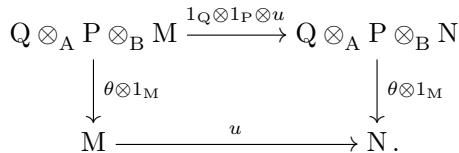
\includegraphics[keepaspectratio]{images/part001_2598f5b2.jpg}}

定理 1. —— 设 A 与 B 是 k-代数，P 是一个 \((A,B)_{k}\)-双模。把 \((B,A)_{k}\)-双模 \(\operatorname{Hom}_{\mathrm{A}}(\mathrm{P},\mathrm{A}_{s})\) 记作 \(P^{*}\)。下列性质等价：

\begin{enumerate}
\def\labelenumi{(\roman{enumi})}
\item
  \((\mathrm{A},\mathrm{B})_k\)-双模 P 是可逆的。
\item
  A-模 P 是投射的、有限生成的且是生成模，且映射 \(b \mapsto b_{P}\)（从 B 到 \(\operatorname{End}_{\mathrm{A}}(\mathrm{P})^{\circ}\)）是 k-代数同构。
\item
  右 B-模 P 是投射的、有限生成的且是生成模，且映射 \(a \mapsto a_{P}\)（从 A 到 \(\operatorname{End}_{\mathrm{B}}(\mathrm{P})\)）是 k-代数同构。若这些性质成立，则同态
\end{enumerate}

\[
\Theta : \mathrm{P} ^ {*} \otimes \mathrm{P} \to {} _ {s} \mathrm{B} _ {d} \quad \text{且} \quad \Lambda : \mathrm{P} \otimes \mathrm{P} ^ {*} \to {} _ {s} \mathrm{A} _ {d}
\]

均为同构，于是 \((\mathrm{B},\mathrm{A})_k\)-双模 \(\mathrm{P}^*\) 是 \(\mathrm{P}\) 的一个逆。

若性质 (ii) 成立，则 P 是一个可逆 \((\mathrm{A},\mathrm{B})_{k}\)-双模，其逆为 \(P^{*}\)（VIII, 第 98 页，命题 2 及第 98 页，命题 3）。这就证明了 (ii) 蕴含 (i) 以及最后一个断言。

设 \((\mathrm{A},\mathrm{B})_{k}\)-双模 P 是可逆的。那么 A-模 P 是生成模（VIII, 第 98 页，命题 3, (iii) \(\Rightarrow\) (i)）。因而它是忠实的且平衡的（VIII, 第 82 页，定理 2），于是映射 \(a \mapsto a_{p}\)（从 A 到 \(\operatorname{End}_{\mathrm{B}}(\mathrm{P})\)）是双射。

现在证明映射 \(b \mapsto b_{\mathrm{P}}\)（从 B 到 \(\mathrm{End}_{\mathrm{A}}(\mathrm{P})\)）是双射。设 Q 是一个 \((\mathrm{B},\mathrm{A})_k\)-双模，它是 P 的逆。设 \(u \in \mathrm{End}_{\mathrm{A}}(\mathrm{P})\)；则 \(1_{\mathrm{Q}} \otimes u\) 是左 B-模 \(\mathbf{Q} \otimes_{\mathrm{A}} \mathbf{P}\) 的一个自同态。由于 \((\mathrm{B},\mathrm{B})_k\)-双模 \(\mathbf{Q} \otimes_{\mathrm{A}} \mathbf{P}\) 同构于 \({}_s\mathbf{B}_d\)，存在 B 中唯一的元素 \(b\)，使得 \(1_{\mathrm{Q}} \otimes u\) 是以 \(b\) 为比的、右 B-模 \(\mathbf{Q} \otimes_{\mathrm{A}} \mathbf{P}\) 的位似。于是我们有 \(1_{\mathrm{Q}} \otimes (u - b_{\mathrm{P}}) = 0\)。从而由引理 1 得 \(u = b_{\mathrm{P}}\)；这就证明了映射 \(b \mapsto b_{\mathrm{P}}\)（从 B 到 \(\operatorname{End}_{\mathrm{A}}(\mathrm{P})\)）是双射。

于是由 VIII, 第 98 页的命题 2，A-模 P 是投射的且有限生成的。这样我们就证明了 (i) 与 (ii) 的等价性。

交换 A 与 B 的角色，即得 (i) 与 (iii) 的等价性，命题证毕。

推论 1. —— 设 A 与 B 是森田等价的 k-代数，P 是一个可逆 \((A,B)_{k}\)-双模。存在一个同构 \(\varphi\)，从 A 的中心 \(Z(A)\) 到 B 的中心，它由关系式 \(\varphi(z)_{\mathrm{P}} = z_{\mathrm{P}}\)（对每个 \(z \in Z(A)\)）确定。\((A,B)_{k}\)-双模 P 的自同构是诸位似 \(z_{P}\)，其中 z 是 \(Z(A)\) 的一个可逆元素。

给定定理 1，这由 VIII, 第 97 页的注 2 得出。

推论 2. —— 设 A 与 B 是森田等价的 k-代数，P 是一个可逆 \((\mathrm{A},\mathrm{B})_{k}\)-双模。每个与 P 互逆的 \((\mathrm{B},\mathrm{A})_{k}\)-双模都同构于 P 的对偶 \(\mathrm{P}^{*}=\mathrm{Hom}_{\mathrm{A}}(\mathrm{P},\mathrm{A})\)。更精确地说，设 Q 是一个作为 P 的逆的 \((\mathrm{B},\mathrm{A})_{k}\)-双模，\(\lambda:P\otimes_{B}Q\to_{s}A_{d}\) 是 \((\mathrm{A},\mathrm{A})_{k}\)-双模的一个同构。存在唯一的映射 \(\tau:\mathrm{Q}\to\mathrm{P}^{*}\)，它由关系式 \(\langle p,\tau(q)\rangle=\lambda(p\otimes q)\)（\(p\in P\)，\(q\in Q\)）确定，且 \(\tau\) 是 \((\mathrm{B},\mathrm{A})_{k}\)-双模的同构。

映射 \(\tau\) 的存在性与唯一性是明显的。它是 \((\mathrm{B},\mathrm{A})_{k}\)-双模的同态，并且我们有 \(\lambda=\Lambda\circ(1_{\mathrm{P}}\otimes\tau)\)。由于 \(\lambda\) 与 \(\Lambda\) 都是 \((\mathrm{A},\mathrm{A})_{k}\)-双模的同构（VIII, 第 101 页，定理 1），\(1_{P}\otimes\tau\) 亦是。由引理 1，映射 \(\tau\) 是双射。

注. —— 在该推论的假设下，设 q 是 Q 的一个元素，使得 \(\lambda(p \otimes q) = 0\)（对每个 \(p \in P\)）。那么我们有 \(\tau(q) = 0\)，即 q = 0。同样，若 p 是 P 的一个元素，使得 \(\lambda(p \otimes q) = 0\)（对每个 \(q \in Q\)），则 p = 0。

例. —— 1) 设 B 是一个 \(k\)-代数，\(n\) 是一个 \(\geqslant 1\) 的整数，A 是 \(k\)-代数 \(\mathbf{M}_n(\mathrm{B})\)。右 B-模 \(\mathrm{P} = \mathrm{B}_d^n\) 是投射的、有限生成的且是生成模，并且 A 可以等同于 P 的自同态代数（II, §10, No.~7, 第 349 页）。由定理 1，\((\mathrm{A},\mathrm{B})_k\)-双模 P 是可逆的。于是代数 B 与 \(\mathbf{M}_n(\mathrm{B})\) 是森田等价的。

\begin{enumerate}
\def\labelenumi{\arabic{enumi})}
\setcounter{enumi}{1}
\tightlist
\item
  *设 A 是一个交换 \(k\)-代数，P 是一个 A-模。我们把 P 视为一个两个作用律相等的 \((A, A)_k\)-双模。若 \((A, A)_k\)-双模 P 是可逆的，则 A-模 P 是有限生成的（定理 1）。由《交换代数》II, §5, No.~4, 第 114 页的定理 3，下列性质等价：
\end{enumerate}

\begin{enumerate}
\def\labelenumi{(\roman{enumi})}
\item
  \((\mathrm{A},\mathrm{A})_{k}\)-双模 P 是可逆的。
\item
  存在一个 A-模 \(\mathrm{Q}\)，使得 \(\mathrm{P} \otimes_{\mathrm{A}} \mathrm{Q}\) 同构于 \(\mathrm{A}\)。
\item
  A-模 P 是投射的、有限生成的，且秩为 1。 *
\end{enumerate}

\subsection{模的森田对应}

在本小节中，字母 A 与 B 表示森田等价的 k-代数，P 表示一个可逆 \((A,B)_{k}\)-双模。取定一个与 P 互逆的 \((B,A)_{k}\)-双模 Q 以及同构

\[
\lambda : \mathrm{P} \otimes_ {\mathrm{B}} \mathrm{Q} \rightarrow {} _ {s} \mathrm{A} _ {d} \quad \text { and } \quad \theta : \mathrm{Q} \otimes_ {\mathrm{A}} \mathrm{P} \rightarrow {} _ {s} \mathrm{B} _ {d}.
\]

对每个左 B-模 V，用 \(\theta_{V}\) 表示 B-模同态 \(\theta\otimes1_{V}:Q\otimes_{A}P\otimes_{B}V\to V\)；由于 \(\theta\) 是同构，它是同构。同样，对每个左 A-模 M，用 \(\lambda_{M}\) 表示 A-模同态 \(\lambda\otimes1_{M}:P\otimes_{B}Q\otimes_{A}M\to M\)；由于 \(\lambda\) 是同构，它是同构。

定理 2（森田）. —— a) 设 V 与 W 是左 B-模。映射 \(g \mapsto 1_{\mathrm{P}} \otimes g\) 是从 \(\operatorname{Hom}_{\mathrm{B}}(\mathrm{V}, \mathrm{W})\) 到 \(\operatorname{Hom}_{\mathrm{A}}(\mathrm{P} \otimes_{\mathrm{B}} \mathrm{V}, \mathrm{P} \otimes_{\mathrm{B}} \mathrm{W})\) 的双射。逆双射把 \(\operatorname{Hom}_{\mathrm{A}}(\mathrm{P} \otimes_{\mathrm{B}} \mathrm{V}, \mathrm{P} \otimes_{\mathrm{B}} \mathrm{W})\) 的元素 h 映为元素 \(\theta_{\mathrm{W}} \circ (1_{\mathrm{Q}} \otimes h) \circ \theta_{\mathrm{V}}^{-1}\)，它属于 \(\operatorname{Hom}_{\mathrm{B}}(\mathrm{V}, \mathrm{W})\)。

\begin{enumerate}
\def\labelenumi{\alph{enumi})}
\setcounter{enumi}{1}
\tightlist
\item
  每个左 A-模 M 都同构于形如 \(\mathrm{P} \otimes_{\mathrm{B}} \mathrm{V}\) 的模，其中 V 是左 B-模。
\end{enumerate}

设 V 与 W 是左 B-模。由 VIII, 第 101 页的引理 1，映射 \(\varphi : g \mapsto 1_{\mathrm{P}} \otimes g\)（从 \(\mathrm{Hom}_{\mathrm{B}}(\mathrm{V}, \mathrm{W})\) 到 \(\mathrm{Hom}_{\mathrm{A}}(\mathrm{P} \otimes_{\mathrm{B}} \mathrm{V}, \mathrm{P} \otimes_{\mathrm{B}} \mathrm{W})\)）是单射。交换 P 与 Q（以及 A 与 B）的角色，可见映射 \(\psi : h \mapsto 1_{\mathrm{Q}} \otimes h\)（从 \(\mathrm{Hom}_{\mathrm{A}}(\mathrm{P} \otimes_{\mathrm{B}} \mathrm{V}, \mathrm{P} \otimes_{\mathrm{B}} \mathrm{W})\) 到 \(\mathrm{Hom}_{\mathrm{A}}(\mathrm{Q} \otimes_{\mathrm{A}} \mathrm{P} \otimes_{\mathrm{B}} \mathrm{V}, \mathrm{Q} \otimes_{\mathrm{A}} \mathrm{P} \otimes_{\mathrm{B}} \mathrm{W})\)）也是单射。而复合 \(\psi \circ \varphi\) 是映射 \(g \mapsto \theta_{\mathrm{W}}^{-1} \circ g \circ \theta_{\mathrm{V}}\)。它是双射，因而 \(\psi\) 也是。于是 \(\varphi\) 是双射，其逆是映射 \(h \mapsto \theta_{\mathrm{W}} \circ (1_{\mathrm{Q}} \otimes h) \circ \theta_{\mathrm{V}}^{-1}\)。

断言 b) 由 \(\lambda_{\mathrm{M}}\) 是从 \(\mathrm{P} \otimes_{\mathrm{B}} \otimes_{\mathrm{A}} \otimes_{\mathrm{M}}\) 到 \(\mathrm{M}\) 的同构这一事实得出。

设 V 是一个左 B-模，W 是 V 的一个子模。由于 B-模 P 是投射的（VIII, 第 101 页，定理 1），从 \(P \otimes_{B} W\) 到 \(P \otimes_{B} V\) 的典范映射是单射。我们借此映射把 \(P \otimes_{B} W\) 与它在 \(P \otimes_{B} V\) 中的像等同起来。当 P 与 B 分别换成 Q 与 A 时，我们采用类似的约定。

命题 5. —— 设 V 是一个左 B-模。映射 \(W \mapsto P \otimes_{B} W\) 是从 V 的 B-子模之集（按包含关系排序）到 \(P \otimes_{B} V\) 的 A-子模之集（按包含关系排序）的同构。逆同构把 \(P \otimes_{B} V\) 的 A-子模 N 映为 \(\theta_{V}\) 作用下 B-子模 \(Q \otimes_{A} N\)（\(Q \otimes_{A} P \otimes_{B} V\) 的子模）的像。

用 \(D_{\mathrm{B}}(\mathrm{V})\) 表示 V 的按包含关系排序的 B-子模之集，并同样地定义集合 \(D_{\mathrm{A}}(\mathrm{P}\otimes_{\mathrm{B}}\mathrm{V})\) 与 \(D_{\mathrm{B}}(\mathrm{Q}\otimes_{\mathrm{A}}\mathrm{P}\otimes_{\mathrm{B}}\mathrm{V})\)。设 \(\varphi:D_{\mathrm{B}}(\mathrm{V})\to D_{\mathrm{A}}(\mathrm{P}\otimes_{\mathrm{B}}\mathrm{V})\) 是映射 \(W\mapsto P\otimes_{B}W\)，\(\psi\) 是从 \(D_{\mathrm{A}}(\mathrm{P}\otimes_{\mathrm{B}}\mathrm{V})\) 到 \(D_{\mathrm{B}}(\mathrm{Q}\otimes_{\mathrm{A}}\mathrm{P}\otimes_{\mathrm{B}}\mathrm{V})\) 的映射，由 \(N\mapsto Q\otimes_{A}N\) 给出。它们都是递增映射，且复合 \(\psi\circ\varphi\) 是映射 \(W\mapsto\theta_{\mathrm{V}}^{-1}(\mathrm{W})\)，后者是双射。于是 \(\varphi\) 是单射，而 \(\psi\) 是满射。把 B 换成 A、V 换成 \(P\otimes_{B}V\)，即见 \(\psi\) 也是单射。从而 \(\varphi\) 与 \(\psi\) 都是双射，且 \(\varphi\) 的逆映射正是命题中所描述的那个。

例. —— 1) 把 VIII, 第 104 页的命题 5 应用于特殊情形 \(\mathrm{V} = \mathrm{B}_s\)。

\begin{enumerate}
\def\labelenumi{\alph{enumi})}
\item
  映射 \(J \mapsto PJ\) 是从 B 的左理想的有序集 \(\mathrm{D}(\mathrm{B}_{s})\) 到 P 的 A-子模的有序集 \(\mathrm{D}(\mathrm{P})\) 的同构。逆映射把 P 的 A-子模 M 映为 B 的左理想 \(\mathrm{J}(\mathrm{M})\)，它由 B 中使 M 包含 Pb 的元素 b 组成。
\item
  映射 \(K \mapsto KP\) 是从 A 的右理想的有序集 \(\mathrm{D}(A_{d})\) 到 P 的 B-子模的有序集 \(\mathrm{D}(P)\) 的同构。逆映射把 P 的 B-子模 V 映为 A 的右理想 \(\mathrm{K}(V)\)，它由 A 中使 V 包含 aP 的元素 a 组成。
\end{enumerate}

事实上，A-模 \(P \otimes_{B} B_{s}\) 可以典范地等同于 P。若 J 是 B 的一个左理想，则 \(P \otimes_{B} J\) 在 \(P \otimes_{B} B_{s}\) 中的典范像在此等同下对应于 PJ。于是映射 \(J \mapsto PJ\) 是从 \(D(B_{s})\) 到 \(D(P)\) 的有序集同构。设 \(J \in D(B_{s})\)。用 \(J'\) 表示 B 中使 PJ 包含 Pb 的元素 b 之集。它是 B 的包含 J 的左理想，并且我们有 \(PJ' \subset PJ\)。由于映射 \(J \mapsto PJ\) 是有序集的同构，必然有 \(PJ' = PJ\) 及 \(J = J'\)。这就证明了 a)。

断言 b) 由把断言 a) 应用于可逆 \((\mathrm{B}^{\circ},\mathrm{A}^{\circ})_{k}\)-双模 P 得出。

注意，环 A 是体当且仅当 B-模 P 是单模。

\begin{enumerate}
\def\labelenumi{\arabic{enumi})}
\setcounter{enumi}{1}
\tightlist
\item
  用 \(\mathcal{B}_{\mathrm{A}}\)、\(\mathcal{B}_{\mathrm{B}}\) 与 \(\mathcal{B}_{\mathrm{P}}\) 分别表示 A 的双边理想之集、B 的双边理想之集与 P 的 \((\mathrm{A},\mathrm{B})_k\)-子双模之集。
\end{enumerate}

\begin{enumerate}
\def\labelenumi{\alph{enumi})}
\item
  映射 \(\mathfrak{b} \mapsto \mathrm{P}\mathfrak{b}\) 是从 \(\mathcal{B}_{\mathrm{B}}\) 到 \(\mathcal{B}_{\mathrm{P}}\) 的有序集同构；逆同构把一个 \((\mathrm{A},\mathrm{B})_k\)-子双模 \(\mathrm{P}'\)（\(\mathrm{P}\) 的）映为 \(\mathrm{B}\) 的由元素 \(b\)（使得 \(\mathrm{P}b \subset \mathrm{P}'\)）组成的双边理想。
\item
  映射 \(a \mapsto aP\) 是从 \(B_{A}\) 到 \(B_{P}\) 的有序集同构；逆同构把 P 的 \((A, B)_{k}\)-子双模 \(P'\) 映为 A 的由使 \(aP \subset P'\) 的元素 a 组成的双边理想。
\end{enumerate}

事实上，设 J 是 B 的一个左理想，且 \(P' = PJ\)。那么 \(P'\) 是 P 的 A-子模，并且由例 1，理想 J 由 B 中使 \(Pb \subset P'\) 的元素 b 组成。此外，\(P'\) 是 P 的 \((A, B)_{k}\)-子双模当且仅当 J 是 B 的双边理想。于是 a) 由同前所引得出。

断言 b) 由把断言 a) 应用于可逆 \((\mathrm{B}^{\circ}, \mathrm{A}^{\circ})_{k}\)-双模 P 得出。

命题 6. —— 用 \(\mathcal{B}_{\mathrm{A}}\) 与 \(\mathcal{B}_{\mathrm{B}}\) 表示 A 的双边理想之集与 B 的双边理想之集。

\begin{enumerate}
\def\labelenumi{\alph{enumi})}
\item
  存在一个有序集同构 \(f\)，从 \(\mathcal{B}_{\mathrm{A}}\) 到 \(\mathcal{B}_{\mathrm{B}}\)，它由下列性质确定：若 \(\mathfrak{a}\) 是 \(\mathrm{A}\) 的双边理想，\(\mathfrak{b}\) 是 \(\mathrm{B}\) 的双边理想，则关系 \(f(\mathfrak{a}) = \mathfrak{b}\) 等价于 \(\mathfrak{a}\mathrm{P} = \mathrm{P}\mathfrak{b}\)。
\item
  设环 A 是交换的，从而 A 可等同于 B 的中心（VIII, 第 102 页，推论 1）。同构 \(f: \mathcal{B}_{\mathrm{A}} \to \mathcal{B}_{\mathrm{B}}\) 把 A 的理想 \(\mathfrak{a}\) 映为 B 的双边理想 \(\mathrm{Ba}\)，并且我们有 \(\mathfrak{a} = \mathrm{A} \cap \mathrm{Ba}\)。
\end{enumerate}

断言 a) 由例 2 得出。

现在设 A 是交换的，并把 A 等同于 B 的中心。设 a 是 A 的一个理想。那么 Ba 是 B 的双边理想；我们有 PBa = aP，因此 \(f(a) = \text{Ba}\)。设 \(a'\) 是 A 的理想 \(A \cap Ba\)；它含于 Ba 且包含 a，故 \(Ba'\) 等于 Ba。由于 f 是双射，由此得 \(a' = a\)。

例. —— 3) 设 V 是一个左 B-模。那么上面给出的对应把 B-模 V 的零化理想映为 A-模 \(P \otimes_{B} V\) 的零化理想。事实上，用 a 表示 A-模 \(P \otimes_{B} V\) 的零化理想，用 b 表示 B-模 V 的零化理想。设 W 是 P 的 \((A, B)_{k}\)-子双模，它由使对 V 的每个元素 v 都有 \(p \otimes v = 0\) 的元素组成。我们有包含关系 \(Pb \subset W\)；反之，对每个 \(p \in W\) 与 \(q \in Q\)，我们有 \(\theta(q \otimes p)\) 属于 b。于是，\(D(B_s)\) 的元素 b 对应于 D(P) 的元素 W。同样，\(a \in D(A_d)\) 对应于 W。

\begin{enumerate}
\def\labelenumi{\arabic{enumi})}
\setcounter{enumi}{3}
\tightlist
\item
  对 A 的每个双边理想 \(\mathfrak{a}\)，把 \(\mathbf{M}_n(\mathrm{A})\) 中由系数属于 \(\mathfrak{a}\) 的矩阵组成的子集记作 \(\mathbf{M}_n(\mathfrak{a})\)。它是 \(\mathbf{M}_n(\mathrm{A})\) 的双边理想。我们有 \(\mathbf{M}_n(\mathfrak{a})\mathrm{A}^n = \mathfrak{a}^n = \mathrm{A}^n\mathfrak{a}\)。由命题 6 推出，\(\mathbf{M}_n(\mathrm{A})\) 的每个双边理想都形如 \(\mathbf{M}_n(\mathfrak{a})\)，其中 \(\mathfrak{a}\) 是 A 的双边理想。
\end{enumerate}

注. —— 我们保留上面的假设与记号，并设 \((\mathrm{B},\mathrm{A})_{k}\)-双模 Q 是 A-模 P 的对偶 \(P^{*}\)，同构 \(\lambda\) 与 \(\theta\) 是典范映射 \(\Lambda:P\otimes_{B}P^{*}\to_{s}A_{d}\) 与 \(\Theta:P^{*}\otimes_{A}P\to_{s}B_{d}\)（VIII, 第 101 页，定理 1）。由于 A-模 P 是投射的且有限生成的，对每个 A-模 M 我们有一个典范同构 \(\vartheta_{M}:P^{*}\otimes_{A}M\to\operatorname{Hom}_{A}(P,M)\)（II, §4, No.~2, 第 271 页，推论）。我们把将构造 \(M\mapsto Q\otimes_{A}M\) 换成构造 \(M\mapsto\operatorname{Hom}_{A}(P,M)\) 后对第 3、4 小节结果的改述留给读者。

\subsection{子模的有序集}

在本小节中，A 与 B 是 k-代数，M 是一个左 A-模，V 是一个左 B-模。我们用 \(\mathrm{D}(\mathrm{M})\)（相应地，\(\mathrm{D}(\mathrm{V})\)）表示 M（相应地，V）的按包含关系排序的子模之集。我们设给定了有序集的同构 \(\varphi : \mathrm{D}(\mathrm{V}) \to \mathrm{D}(\mathrm{M})\)。

由森田定理（VIII, 第 103 页，定理 2），在下列情形我们得到这样一个同构：P 是一个可逆 \((\mathrm{A},\mathrm{B})_k\)-双模，M 是 A-模 \(\mathrm{P} \otimes_{\mathrm{B}} \mathrm{V}\)，并且对 V 的每个子模 W，\(\varphi(\mathrm{W})\) 是 \(\mathrm{P} \otimes_{\mathrm{B}} \mathrm{W}\) 在 M 中的典范像。

模 M 的某些性质，或其子模的某些性质，可以用有序集 D(M) 来表达：它们列于表 I 与表 II 中。

模 M 是子模族 \((\mathrm{M}_{i})_{i\in\mathrm{I}}\) 的直和当且仅当我们有 \(M=\sum_{i\in I}M_{i}\) 与 \(M_{i}\cap\sum_{j\neq i}M_{j}=0\)（对每个 \(i\in I\)）。这一注记以及对表 I 的考察给出下面的结果。

命题 7. —— a) 我们有 \(\varphi(0)=0\) 及 \(\varphi(V)=M\)。

\begin{enumerate}
\def\labelenumi{\alph{enumi})}
\setcounter{enumi}{1}
\tightlist
\item
  设 \((\mathrm{V}_i)_{i\in \mathrm{I}}\) 是 V 的一个子模族。我们有
\end{enumerate}

\[
\varphi \left(\sum_ {i \in \mathrm{I}} \mathrm{V} _ {i}\right) = \sum_ {i \in \mathrm{I}} \varphi (\mathrm{V} _ {i}), \quad \varphi \left(\bigcap_ {i \in \mathrm{I}} \mathrm{V} _ {i}\right) = \bigcap_ {i \in \mathrm{I}} \varphi (\mathrm{V} _ {i}).
\]

M 的子模

有序集 D(M)

零子模

D(M) 的最小元

子模 M

D(M) 的最大元

\(\bigcap_{i\in I} M_i\)

下确界 \(\inf_{i\in I} M_i\)

\(\sum_{i\in I} M_i\)

上确界 \(\sup_{i\in I} M_i\)

互补子模

\(\inf(M', M'') = 0, \sup(M', M'') = M\)

M 的单子模

D(M) --- \{0\} 的极小元

M 的极大子模

D(M) --- \{M\} 的极大元

M 的底座 \(\mathscr{S}(M)\)

D(M) --- \{0\} 的极小元之集在 D(M) 中的上确界

\emph{M 的根 \(\Re(M)\)}（VIII, 第 151 页）

D(M) --- \{M\} 的极大元之集在 D(M) 中的下确界

模 M 的性质

D(M) 的性质

M 是诺特模。

有序集 D(M) 是诺特的（《集合论》III, §6, No.~5, 第 190 页）。

M 是阿廷模。

按 ⊃ 排序的集合 D(M) 是诺特的。

M 是不可分解的。

我们有 M ≠ 0，并且不存在 D(M) 的两个非零元素 M\textquotesingle{} 与 M\textquotesingle\textquotesingle{} 满足 inf(M\textquotesingle, M\textquotesingle\textquotesingle) = 0, sup(M\textquotesingle, M\textquotesingle\textquotesingle) = M。

M 是有限生成的。

对 D(M) 中每个以 M 为上界的族 (Mi) i∈I，存在 I 的有限子集 J，使 M = supj∈I Mj。

M 是单模。

Card(D(M)) = 2。

M 是半单的。

M 是 D(M) = \{0\} 的极小元之集在 D(M) 中的上确界。

表 II.

\begin{enumerate}
\def\labelenumi{\alph{enumi})}
\setcounter{enumi}{2}
\tightlist
\item
  B-模 V 是子模族 \((\mathrm{V}_{i})_{i\in\mathrm{I}}\) 的直和当且仅当 M 是子模族 \((\varphi(\mathrm{V}_{i}))_{i\in\mathrm{I}}\) 的直和。
\end{enumerate}

设 \(V'\) 与 \(V''\) 是 \(V\) 的子模，使得 \(V'\) 含于 \(V''\)；令 \(M' = \varphi(V')\)，\(M'' = \varphi(V'')\)，于是 \(M''\) 包含 \(M'\)。用 \([V', V'']\) 表示 \(D(V)\) 中由子模 \(W\)（属于 \(V\)，满足 \(V' \subset W \subset V''\)）组成的区间，并同样地定义区间 \([M', M'']\)（在 \(D(M)\) 中）。映射 \(W \mapsto W/V'\) 是从 \([V', V'']\) 到 \(D(V''/V')\) 的有序集同构；我们同样地定义从 \([M', M'']\) 到 \(D(M''/M')\) 的有序集同构。由于 \(\varphi\) 把区间 \([V', V'']\) 映到 \([M', M'']\)，它定义了一个有序集同构 \(\varphi\)，从 \(D(V''/V')\) 到 \(D(M''/M')\)。我们由此以及表 I 与表 II 推出下面的命题。

命题 8. —— a) 设 V' 与 V'\,' 是 V 的子模，使得 V'\,' 包含 V'。B-模 V'\,'/V' 是单模当且仅当 A-模 \(\varphi(\mathrm{V}^{\prime\prime})/\varphi(\mathrm{V}^{\prime})\) 是单模。

\begin{enumerate}
\def\labelenumi{\alph{enumi})}
\setcounter{enumi}{1}
\item
  若 \(V'\) 是 V 的单子模、极大子模或直因子，则 \(\varphi(V')\) 相应地是 M 的单子模、极大子模或直因子。
\item
  同构 \(\varphi\) 把底座 \(\mathcal{S}(\mathrm{V})\)（\(\mathrm{V}\) 的）变为底座 \(\mathcal{S}(\mathrm{M})\)（\(\mathrm{M}^*\) 的），把根（VIII, 第 151 页，定义 1）\(\Re (\mathrm{V})\)（\(\mathrm{V}\) 的）变为根 \(\Re (\mathrm{M})\)（\(\mathrm{M}_{*}\) 的）
\item
  设 \((\mathrm{V}_{i})_{0\leqslant i\leqslant n}\) 是 V 的子模的一个有限序列。它是 V 的若尔当–赫尔德列当且仅当 \((\varphi(\mathrm{V}_{i})_{0\leqslant i\leqslant n})\) 是 M 的若尔当–赫尔德列。
\end{enumerate}

引理 2. —— 设 H 与 H' 是 V 的子模，满足 \(H \cap H' = 0\)。B-模 H 与 H' 同构当且仅当 A-模 \(\varphi(\mathrm{H})\) 与 \(\varphi(\mathrm{H}')\) 同构。

我们把 \(H+H'\) 等同于乘积 \(H \times H'\)。从 H 到 \(H'\) 的一个同构的图像是 V 的一个子模 \(H''\)，它满足

\[
\mathrm{H} \cap \mathrm{H} ^ {\prime \prime} = \mathrm{H} ^ {\prime} \cap \mathrm{H} ^ {\prime \prime} = 0, \quad \mathrm{H} + \mathrm{H} ^ {\prime} = \mathrm{H} + \mathrm{H} ^ {\prime \prime} = \mathrm{H} ^ {\prime} + \mathrm{H} ^ {\prime \prime};\tag{17}
\]

反之，每个具有这些性质的子模是从 H 到 \(H'\) 的一个同构的图像。由命题 7，关系 \(H \cap H' = 0\) 等价于 \(\varphi(\mathrm{H}) \cap \varphi(\mathrm{H}') = 0\)，而关系式 (17) 等价于关系式

\[
\varphi (\mathrm{H}) \cap \varphi (\mathrm{H} ^ {\prime \prime}) = \varphi (\mathrm{H} ^ {\prime}) \cap \varphi (\mathrm{H} ^ {\prime \prime}) = 0,
\]

\[
\varphi (\mathrm{H}) + \varphi (\mathrm{H} ^ {\prime}) = \varphi (\mathrm{H}) + \varphi (\mathrm{H} ^ {\prime \prime}) = \varphi (\mathrm{H} ^ {\prime}) + \varphi (\mathrm{H} ^ {\prime \prime});
\]

引理由此得出。

命题 9. —— 设 S 是 V 的一个单子模，T 是 M 的单子模 \(\varphi(\mathrm{S})\)。若用 \(V_{S}\) 表示 V 的 S 型同型分量，用 \(M_{T}\) 表示 M 的 T 型同型分量，则我们有 \(\varphi(V_{\mathrm{S}})=M_{\mathrm{T}}\)。

V 的每个异于 S 的单子模 \(S'\) 满足 \(S' \cap S = 0\)。因此它同构于 S 当且仅当 \(\varphi(S')\) 同构于 T（引理 2）。而 \(V_{S}\) 是 V 的同构于 S 的单子模之和，\(M_{T}\) 是 M 的同构于 T 的单子模之和。于是命题 9 由命题 7 与命题 8 立即得出。

命题 10. —— a) B-模 V 是阿廷的（相应地，诺特的、不可分解的、单的、有限生成的）当且仅当 M 亦然。

\begin{enumerate}
\def\labelenumi{\alph{enumi})}
\setcounter{enumi}{1}
\item
  B-模 V 具有有限长度当且仅当 A-模 M 具有有限长度，且此时我们有 \(\mathrm{long}_{\mathrm{B}}(\mathrm{V}) = \mathrm{long}_{\mathrm{A}}(\mathrm{M})\)。
\item
  B-模 V 是半单的（相应地，同型的）当且仅当 A-模 M 是半单的（相应地，同型的）。若情形如此，则我们有 \(\text{long}_{\text{B}}(\text{V}) = \text{long}_{\text{A}}(\text{M})\)。
\end{enumerate}

断言 a) 由表 II 中所列的第二条性质得出。

断言 b) 由命题 8, d) 得出。

模 V 是半单的当且仅当它等于其底座 \(\mathcal{S}(V)\)；它是同型的当且仅当存在 V 的一个单子模 S，使得 \(V = V_{S}\)。于是断言 c) 由命题 7, c)、8, c) 与 9（VIII, 第 106 页与第 109 页）得出。

\subsection{森田对应下保持的其他性质}

设 A 与 B 是森田等价的 k-代数，P 是一个可逆 \((A,B)_{k}\)-双模。

命题 11. —— 设

\[
\mathrm{V} ^ {\prime} \xrightarrow {f} \mathrm{V} \xrightarrow {g} \mathrm{V} ^ {\prime \prime}\tag{ε}
\]

是一个由 B-模与 B-线性映射组成的图，并设

\[
(\mathrm{P} \otimes \mathcal {E})
\]

\[
\mathrm{P} \otimes_ {\mathrm{B}} \mathrm{V} ^ {\prime} \xrightarrow {1 _ {\mathrm{P}} \otimes f} \mathrm{P} \otimes_ {\mathrm{B}} \mathrm{V} \xrightarrow {1 _ {\mathrm{P}} \otimes g} \mathrm{P} \otimes_ {\mathrm{B}} \mathrm{V} ^ {\prime \prime}
\]

是相应的 A-模的图。那么 \((\mathcal{E})\) 是正合列当且仅当 \((\mathrm{P} \otimes \mathcal{E})\) 是正合列。

设序列 \((\mathcal{E})\) 是正合的。由于右 B-模 P 是投射的，序列 \((P \otimes \mathcal{E})\) 是正合的（II, §3, No.~6, 第 251 页，命题 5 及 II, §3, No.~7, 第 257 页，推论 6）。

反之，设序列 \((\mathrm{P} \otimes \mathcal{E})\) 是正合的。设 Q 是一个 \((\mathrm{B}, \mathrm{A})_{k}\)-双模，它是 P 的逆，并设 \(\theta : Q \otimes_{A} P \to {}_{s} B_{d}\) 是一个同构。考虑交换图

\[
\begin{array}{c} \mathrm{Q} \otimes_ {\mathrm{A}} \mathrm{P} \otimes_ {\mathrm{B}} \mathrm{V} ^ {\prime} \xrightarrow {1 _ {\mathrm{Q}} \otimes 1 _ {\mathrm{P}} \otimes f} \mathrm{Q} \otimes_ {\mathrm{A}} \mathrm{P} \otimes_ {\mathrm{B}} \mathrm{V} \xrightarrow {1 _ {\mathrm{Q}} \otimes 1 _ {\mathrm{P}} \otimes g} \mathrm{Q} \otimes_ {\mathrm{A}} \mathrm{P} \otimes_ {\mathrm{B}} \mathrm{V} ^ {\prime \prime} \\ \theta \otimes 1 _ {\mathrm{V} ^ {\prime}} \Biggl \downarrow \\ \mathrm{V} ^ {\prime} \xrightarrow {f} \mathrm{V} \xrightarrow {g} \mathrm{V} ^ {\prime \prime}. \end{array}
\]

由于 Q 是投射 A-模且序列 \((\mathrm{P} \otimes \mathcal{E})\) 是正合的，此图的第一行是一个正合列。由于诸竖直箭头都是同构，第二行也是正合的。

推论. —— 设 \(f: V \rightarrow W\) 是一个 B-线性映射。那么 f 是单射（相应地，满射）当且仅当 \(1_{P} \otimes f\) 是。

命题 12. —— 设 V 是一个左 B-模。B-模 V 是投射的（相应地，是生成模、忠实的、*内射的、有限表现的*）当且仅当 A-模 P ⊗\_B V 亦然。

\begin{enumerate}
\def\labelenumi{\alph{enumi})}
\item
  设 V 是投射的。存在一个集合 I，使 V 同构于 \(\mathrm{B}_{s}^{(\mathrm{I})}\) 的一个直因子子模。于是 A-模 \(P \otimes_{B} V\) 同构于 \(\mathrm{P}^{(\mathrm{I})}\) 的一个直因子子模；由于 P 是投射 A-模，\(P \otimes_{B} V\) 亦然。
\item
  设 B-模 V 是生成模。设 M 是一个 A-模。存在一个 B-模 W，使 M 同构于 \(P \otimes_{B} W\)。由 VIII, 第 80 页的定理 1，存在一个集合 I 与一个满射 \(\varphi : V^{(I)} \to W\)。由该推论，映射 \(1_{P} \otimes \varphi\)（从 \(P \otimes (V^{(I)})\) 到 \(P \otimes_{A} W\)）是满射，这给出一个满射 \((P \otimes V)^{(I)} \to M\)。由 VIII, 第 80 页的定理 1，\(P \otimes V\) 是生成 A-模。
\item
  B-模 V 是忠实的当且仅当它的零化理想约化为 0。于是断言 c) 由 VIII, 第 105 页的例 3 得出。
\end{enumerate}

*d) 设 V 是内射的。由 VIII, 第 106 页的注，A-模 \(\mathrm{P} \otimes_{\mathrm{B}} \mathrm{V}\) 同构于 \(\mathrm{Hom}_{\mathrm{B}}(\mathrm{Q}, \mathrm{V})\)，其中 Q 是一个与 A 互逆的 \((\mathrm{B}, \mathrm{A})_k\)-双模。由于 A-模 Q 是投射的，因而是平坦的（X, §1, n° 3, 第 9 页，例 1），由 X, §1, n° 8, 第 18 页，命题 11，A-模 \(\mathrm{Hom}_{\mathrm{B}}(\mathrm{Q}, \mathrm{V})\) 是内射的。

\begin{enumerate}
\def\labelenumi{\alph{enumi})}
\setcounter{enumi}{4}
\item
  设 V 有一个有限表现 \(L_{1} \to L_{0} \to V \to 0\)（X, §1, n° 4, 第 10 页）。用 P 作张量积，我们导出 A-模的一个正合列 \(N_{1}^{\prime} \xrightarrow{u} N_{0}^{\prime} \to P \otimes_{B} V \to 0\)，其中 \(N_{1}^{\prime}\) 与 \(N_{0}^{\prime}\) 是投射的且有限生成的（命题 11 与 a)）。设 \(N_{0}^{\prime\prime}\) 是一个有限生成 A-模，使得模 \(N_{0} = N_{0}^{\prime} \oplus N_{0}^{\prime\prime}\) 是自由的且有限生成的，并设 \(u^{\prime}: N_{1}^{\prime} \oplus N_{0}^{\prime\prime} \to N_{0}\) 是同态 \((u, 1_{N_{0}^{\prime\prime}})\)；于是 \(P \otimes_{B} V\) 可以等同于 \(u^{\prime}\) 的余核。设 \(N_{1}\) 是一个有限生成的自由 A-模，\(p: N_{1} \to N_{1}^{\prime} \oplus N_{0}^{\prime\prime}\) 是一个满射同态；序列 \(N_{1} \xrightarrow{u^{\prime} \circ p} N_{0} \to P \otimes_{B} V \to 0\) 是 A-模 \(P \otimes_{B} V_*\) 的一个有限表现
\item
  设 A-模 \(P \otimes_{B} V\) 是投射的（相应地，是生成模、忠实的、*内射的、有限表现的*）。把上面的结果应用于（交换 A 与 B 以及 P 与 Q 的角色），可见 B-模 \(Q \otimes_{A} P \otimes_{B} V\) 也具有这一性质。于是对同构于它的 B-模 V 同样如此。
\end{enumerate}

推论. —— 环 A 是左阿廷的（相应地，左诺特的）当且仅当环 B 亦然。

由于 B 的左理想的有序集与 P 的 A-子模之集之间的同构，环 B 是左阿廷的（相应地，左诺特的）当且仅当 A-模 P 是阿廷的（相应地，诺特的）。而由 VIII, 第 101 页的定理 1，A-模 P 是生成模且有限生成；特别地，\(A_{s}\) 同构于 \(P^{n}\) 的一个直因子（对一个整数 \(n \geqslant 1\)）。因此，P 是阿廷的（相应地，诺特的）当且仅当 A 是左阿廷的（相应地，左诺特的）。

\subsection{代数的森田等价}

命题 13. —— a) 若两个 k-代数是森田等价的，则它们的中心是同构的 k-代数。

\begin{enumerate}
\def\labelenumi{\alph{enumi})}
\setcounter{enumi}{1}
\item
  两个交换 \(k\)-代数森田等价当且仅当它们同构。
\item
  两个都是体的 k-代数森田等价当且仅当它们同构。
\item
  对 \(i = 1,2\)，设 \(\mathrm{A}_i\) 与 \(\mathrm{B}_i\) 是森田等价的 \(k\)-代数，\(\mathrm{P}_i\) 是一个可逆 \((\mathrm{A}_i,\mathrm{B}_i)_k\)-双模。令 \(\mathrm{A} = \mathrm{A}_1\otimes_k\mathrm{A}_2\)，\(\mathrm{B} = \mathrm{B}_1\otimes_k\mathrm{B}_2\)，\(\mathrm{P} = \mathrm{P}_1 \otimes_k \mathrm{P}_2\)。\(k\)-代数 A 与 B 是森田等价的，且 P 是一个可逆 \((\mathrm{A}, \mathrm{B})_k\)-双模。
\item
  若 A 与 B 是森田等价的 \(k\)-代数，且 \(k'\) 是一个交换 \(k\)-代数，则 \(k'\)-代数 \(\mathrm{A}_{(k')}\) 与 \(\mathrm{B}_{(k')}\) 是森田等价的。
\end{enumerate}

断言 a) 由 VIII, 第 102 页的推论 1 得出，并蕴含 b)。

设 \(\mathrm{K}\) 与 \(\mathrm{L}\) 是都是体的 \(k\)-代数，\(\mathrm{P}\) 是一个可逆 \((\mathrm{K},\mathrm{L})_k\)-双模。右 \(\mathrm{L}\)-向量空间 \(\mathrm{P}\) 是一个单模（VIII, 第 104 页），因而是 1 维的，于是 \(k\)-代数 \(\operatorname{End}_{\mathrm{L}}(\mathrm{P})\) 与 \(\mathrm{L}\) 同构。由 VIII, 第 101 页的定理 1，映射 \(a\mapsto a_{\mathrm{P}}\)（从 \(\mathrm{K}\) 到 \(\operatorname{End}_{\mathrm{L}}(\mathrm{P})\)）是一个同构。因此，体 \(\mathrm{K}\) 与 \(\mathrm{L}\) 在 \(k\) 上同构；断言 c) 得证。

在 d) 的假设下，设 \(Q_{i}\)（i = 1, 2）是一个 \((\mathrm{B}_{i}, \mathrm{A}_{i})_{k}\)-双模，与 \(P_{i}\) 互逆。用 Q 表示 \((\mathrm{B}, \mathrm{A})_{k}\)-双模 \(Q_{1} \otimes_{k} Q_{2}\)。考虑典范 k-线性同构 \((\mathrm{P}_{1} \otimes_{k} \mathrm{P}_{2}) \otimes_{k} (\mathrm{Q}_{1} \otimes_{k} \mathrm{Q}_{2}) \to (\mathrm{P}_{1} \otimes_{k} \mathrm{Q}_{1}) \otimes_{k} (\mathrm{P}_{2} \otimes_{k} \mathrm{Q}_{2})\)；在过渡到商时，它定义一个态射

\[
\left(\mathrm{P} _ {1} \otimes_ {k} \mathrm{P} _ {2}\right) \otimes_ {\mathrm{B}} \left(\mathrm{Q} _ {1} \otimes_ {k} \mathrm{Q} _ {2}\right)\rightarrow \left(\mathrm{P} _ {1} \otimes_ {\mathrm{B} _ {1}} \mathrm{Q} _ {1}\right) \otimes_ {k} \left(\mathrm{P} _ {2} \otimes_ {\mathrm{B} _ {2}} \mathrm{Q} _ {2}\right)
\]

它是 (A,A)-线性的。反之，逆同构 \((\mathrm{P}_{1}\otimes_{k}\mathrm{Q}_{1})\otimes_{k}(\mathrm{P}_{2}\otimes_{k}\mathrm{Q}_{2})\to(\mathrm{P}_{1}\otimes_{k}\mathrm{P}_{2})\otimes_{k}(\mathrm{Q}_{1}\otimes_{k}\mathrm{Q}_{2})\) 定义一个 (A,A)-线性态射 \((\mathrm{P}_{1}\otimes_{\mathrm{B}_{1}}\mathrm{Q}_{1})\otimes_{k}(\mathrm{P}_{2}\otimes_{\mathrm{B}_{2}}\mathrm{Q}_{2})\to(\mathrm{P}_{1}\otimes_{k}\mathrm{P}_{2})\otimes_{\mathrm{B}}(\mathrm{Q}_{1}\otimes_{k}\mathrm{Q}_{2})\)。这两个态射互为逆映射，从而都是同构。由于 \((\mathrm{A}_{i},\mathrm{A}_{i})\)-双模 \(P_{i}\otimes_{B_{i}}Q_{i}\) 同构于 \(A_{i}\)，我们得到一个 (A,A)-线性同构 \(P\otimes_{B}Q\to A\)。我们同样得到一个 (B,B)-线性同构 \(Q\otimes_{A}P\to B\)，这就完成了 d) 的证明。

在 e) 的假设下，设 P 是一个可逆 \((\mathrm{A},\mathrm{B})_{k}\)-双模；则 \(\mathrm{P}_{(k^{\prime})}\) 是一个可逆 \((\mathrm{A}_{(k^{\prime})},\mathrm{B}_{(k^{\prime})})_{k^{\prime}}\)-双模。

设 A 是一个 k-代数，e 是 A 中的一个幂等元。集合 eAe 赋以由 A 的加法、乘法与 k 的作用所诱导的运算，是一个以 e 为单位元的 k-代数。

命题 14. —— 设 A 与 B 是 k-代数。那么 A 与 B 森田等价当且仅当存在一个整数 \(n \geqslant 1\) 与一个方阵 \(e = (e_{ij})\)（在 \(\mathbf{M}_{n}(\mathbf{B})\) 中），满足下列条件：

\begin{enumerate}
\def\labelenumi{(\roman{enumi})}
\item
  我们有 \(e^2 = e\)。
\item
  由诸元素 \(e_{ij}\) 生成的 B 的双边理想等于 B。
\item
  \(k\)-代数 A 同构于 \(e\mathbf{M}_n(\mathrm{B})e\)。
\end{enumerate}

若条件 (i) 与 (ii) 满足，则 \((e\mathbf{M}_n(\mathrm{B})e,\mathrm{B})_k\)-双模 \(e\mathrm{B}_d^n\) 是可逆的。

鉴于定理 1（VIII, 第 101 页），k-代数 A 与 B 森田等价当且仅当它同构于一个投射的、有限生成的且是生成模的右 B-模的自同态代数。于是该命题由下面的引理 3 与引理 4 得出。

引理 3. —— 一个右 B-模 P 是投射的、有限生成的且是生成模，当且仅当存在一个整数 \(n \geqslant 0\) 与一个幂等元 \(e = (e_{ij})\)（在 \(\mathbf{M}_n(\mathrm{B})\) 中），具有下列性质：

\begin{enumerate}
\def\labelenumi{(\roman{enumi})}
\item
  B-模 P 同构于 \(e\mathrm{B}_d^n\)。
\item
  由诸元素 \(e_{ij}\) 生成的 B 的双边理想等于 B。
\end{enumerate}

设 P 是一个右 B-模。那么 P 是投射的且有限生成的，当且仅当它同构于一个形如 \(B_{d}^{n}\) 的 B-模（n 是一个 \(\geqslant 0\) 的整数）的直因子子模（II, §2, No.~2, 第 232 页，推论 1）。若我们把 k-代数 \(\mathbf{M}_{n}(\mathrm{B})\) 与 \(\operatorname{End}(\mathrm{B}_{d}^{n})\) 等同起来，则这就意味着存在 \(\mathbf{M}_{n}(\mathrm{B})\) 中的一个幂等元 e，使 P 同构于 \(eB_{d}^{n}\)。

B-模 P 是生成模当且仅当它的迹理想 \(\tau(\mathrm{P})\) 等于 B，即 \(\tau(e\mathrm{B}_{d}^{n})=\mathrm{B}\)（VIII, 第 80 页，定理 1）。设 \(x_{1},\ldots,x_{n}\) 是 \(B_{d}^{n}\) 中对应于矩阵 e 的各列的元素，并设 \(x_{i}^{*}\)（对 \(1\leqslant i\leqslant n\)）是线性形式 \((b_{1},\ldots,b_{n})\mapsto b_{i}\)（在 \(eB_{d}^{n}\) 上）。族 \((x_{1},\ldots,x_{n})\) 生成 B-模 \(eB_{d}^{n}\)，而族 \((x_{1}^{*},\ldots,x_{n}^{*})\) 生成它的对偶。而我们由 \(\langle x_{i}^{*},x_{j}\rangle=e_{ij}\)，故 \(\tau(eB_{d}^{n})\) 是由诸 \(e_{ij}\) 生成的 B 的双边理想。这就证明了引理 3。

引理 4. —— 设 V 是一个 B-模，E 是 V 的自同态 k-代数。设 e 是 V 的一个投影算子，P 是 e 的像。把 \(v \in eEe\) 映到 B-模 P 的自同态 \(x \mapsto v(x)\) 的映射是从 eEe 到 \(\operatorname{End}_{\mathrm{B}}(\mathrm{P})\) 的 k-代数同构。

用 \(\varphi:eEe\to\operatorname{End}_{\mathrm{B}}(\mathrm{P})\) 表示陈述中所描述的映射；它是一个 k-代数同态。设 \(u\in\operatorname{End}_{\mathrm{B}}(\mathrm{P})\)。用 v 表示由 \(v(x)=u(e(x))\)（\(x\in V\)）定义的 V 的自同态。我们有 \((eve)(x)=u(x)\)（对 \(x\in P\)），即 \(\varphi(eve)=u\)。于是 \(\varphi\) 是满射。设 w 是 \(\varphi\) 的核的一个元素；w 在 e 的核上与像上的限制均为零，故 w 为零，这就证明 \(\varphi\) 是单射。

例. —— 1) 设 A 是一个 k-代数，e 是 A 中满足 AeA = A 的幂等元。k-代数 eAe 可以等同于子模 \(eA_{d}\)（\(A_{d}\) 的）的自同态 k-代数（引理 4）。由于 AeA = A，由命题 14 推出 \(eA_{d}\) 是一个可逆 \((eAe, A)_{k}\)-双模，于是 \(k\)-代数 eAe 与 A 是森田等价的。此外，森田定理（VIII, 第 103 页）蕴含下面的结果：

\begin{enumerate}
\def\labelenumi{\alph{enumi})}
\item
  设 M 与 N 是左 A-模。每个从 eM 到 eN 的 eAe-线性映射都唯一地扩张为一个从 M 到 N 的 A-线性映射。
\item
  k-代数 eAe 上的每个左模都同构于形如 eM 的模，其中 M 是一个左 A-模。
\end{enumerate}

\begin{enumerate}
\def\labelenumi{\arabic{enumi})}
\setcounter{enumi}{1}
\tightlist
\item
  设 A 是一个 k-代数，\(n \geqslant 1\) 是一个整数。我们把矩阵代数 \(\mathbf{M}_{n}(\mathrm{A})\) 等同于右 A-模 \(A_{d}^{n}\) 的自同态代数。我们已经看到 A 与 \(\mathbf{M}_{n}(\mathrm{A})\) 是森田等价的。对每个左 A-模 M，把 \(A_{d}^{n} \otimes_{A} M\) 与 \(M^{n}\) 等同起来。于是代数 \(\mathbf{M}_{n}(\mathrm{A})\) 在 \(M^{n}\) 上有一个左作用，并且我们有
\end{enumerate}

\[
(a \cdot m) _ {i} = \sum_ {j = 1} ^ {n} a _ {i j} m _ {j}
\]

其中 \(a = (a_{ij})\) 属于 \(\mathbf{M}_n(\mathrm{A})\)，\(m = (m_i)\) 属于 \(\mathrm{M}^n\)。森田定理蕴含下面的结果：

\begin{enumerate}
\def\labelenumi{\alph{enumi})}
\item
  代数 \(\mathbf{M}_n(\mathrm{A})\) 上的每个左模都同构于形如 \(\mathrm{M}^n\) 的模，其中 \(\mathrm{M}\) 是一个左 A-模。
\item
  设 \(\mathrm{M}\) 是一个左 A-模。映射 \(\mathrm{N} \mapsto \mathrm{N}^n\) 是从 \(\mathrm{M}\) 的 A-子模之集到 \(\mathbf{M}_n(\mathrm{A})\)-子模之集（\(\mathrm{M}^n\) 的）的双射。
\item
  设 M 与 N 是左 A-模。对 A-线性映射 \(g: \mathrm{M} \to \mathrm{N}\)，用 \(g_{n}\) 表示映射 \((m_{i}) \mapsto (g(m_{i}))\)（从 \(\mathrm{M}^{n}\) 到 \(\mathrm{N}^{n}\)）。那么映射 \(g \mapsto g_{n}\) 是从 \(\operatorname{Hom}_{\mathrm{A}}(\mathrm{M}, \mathrm{N})\) 到 \(\operatorname{Hom}_{\mathbf{M}_{n}(\mathrm{A})}(\mathrm{M}^{n}, \mathrm{N}^{n})\) 的双射。
\item
  设 M 是一个左 A-模。模 \(M^{n}\)（在环 \(\mathbf{M}_{n}(\mathrm{A})\) 上）是不可分解的（相应地，半单的、单的、阿廷的、诺特的、有限生成的）当且仅当 A-模 M 亦然。
\end{enumerate}

\begin{enumerate}
\def\labelenumi{\arabic{enumi})}
\setcounter{enumi}{2}
\tightlist
\item
  设 A 是一个主理想整环，L 是一个非零的、有限生成的自由 A-模。设 B 是 L 的自同态环；则 L 是一个可逆 \((\mathrm{A},\mathrm{B})_{\mathbf{Z}}\)-双模，且环 A 与 B 是森田等价的。由森田定理、命题 10, a)（VIII, 第 109 页）以及有限生成 A-模的结构定理（VII, §4, No.~4, 第 19 页，定理 2），每个有限生成 B-模都同构于 \(\oplus_{i=1}^{m}(\mathrm{L}/\mathfrak{a}_{i}\mathrm{L})\)，其中 m 是一个自然数，诸 \(a_{i}\) 是 A 的理想，满足 \(a_{1} \subset a_{2} \subset \cdots \subset a_{m}\) 且 \(a_{m} \neq A\)；整数 m 与诸理想 \(a_{i}\) 是唯一确定的。由 VIII, 第 105 页的命题 6，B 的每个双边理想都形如 dB，其中 d 是 A 的一个元素。
\end{enumerate}

\BourbakiExercises{习题}

\begin{enumerate}
\def\labelenumi{\arabic{enumi})}
\tightlist
\item
  设 A、B 是环，P 是一个 (A, B)-双模，Q 是一个 (B, A)-双模。设 \(\varphi: P \otimes_{B} Q \to A\) 是一个 (A, A)-双模同态，\(\psi: Q \otimes_{A} P \to B\) 是一个 (B, B)-双模同态，满足对 P 中的 x, y 与 Q 中的 u, v 有 \(\varphi(x \otimes u)y = x\psi(u \otimes y)\) 及 \(u\varphi(x \otimes v) = \psi(u \otimes x)v\)。设 \(\varphi\) 是满射。
\end{enumerate}

\begin{enumerate}
\def\labelenumi{\alph{enumi})}
\item
  证明 A-模 P 是生成模。
\item
  证明 \(\varphi\) 是同构。
\item
  构造 Q 与 \(\operatorname{Hom}_{\mathbb{B}}(\mathrm{P}, \mathrm{B})\) 之间的一个 (B, A)-双模同构。
\end{enumerate}

\begin{enumerate}
\def\labelenumi{\arabic{enumi})}
\setcounter{enumi}{1}
\item
  设 M、N 是 A-模，m、n 是 \(\geqslant 1\) 的整数。设 M 是 \(N^{n}\) 的一个直因子，N 是 \(M^{m}\) 的一个直因子；证明环 \(\operatorname{End}_{\mathrm{A}}(\mathrm{M})\) 与 \(\operatorname{End}_{\mathrm{A}}(\mathrm{N})\) 是森田等价的。
\item
  设 A 是一个环，G 是一个用加法记号表示的交换群。映射 \(T: A \to G\) 称为迹型的，若它是一个加群同态并且对 A 中的所有 a, b 有 \(T(ab) = T(ba)\)。
\end{enumerate}

\begin{enumerate}
\def\labelenumi{\alph{enumi})}
\item
  设 \(T : A \to G\) 是一个迹型映射，P 是一个投射的且有限生成的右 A-模。证明存在唯一的迹型映射 \(\mathrm{T}_{\mathrm{P}} : \mathrm{End}_{\mathrm{A}}(\mathrm{P} \oplus \mathrm{A}_{d}) \to \mathrm{G}\)，它在 \(\mathrm{A} = \mathrm{End}_{\mathrm{A}}(\mathrm{A}_{d})\) 上的限制为 T。
\item
  设 A 与 B 是森田等价的环，G 是一个交换群。构造从 A 到 G 的迹型映射与从 B 到 G 的迹型映射之间的一个双射对应。
\end{enumerate}

\begin{enumerate}
\def\labelenumi{\arabic{enumi})}
\setcounter{enumi}{3}
\tightlist
\item
  设 A 与 B 是环，P 是一个可逆 (A,B)-双模。用 \(\mathcal{B}_{\mathrm{A}}\)（相应地，\(B_{B}\)）表示 A（相应地，B）的双边理想之集，用 \(f: B_{A} \to B_{B}\) 表示命题 6（VIII, 第 105 页）中定义的有序集同构。
\end{enumerate}

\begin{enumerate}
\def\labelenumi{\alph{enumi})}
\item
  设 \(\mathfrak{a}\) 是 A 的一个理想。证明环 A/ \(\mathfrak{a}\) 与 B/f( \(\mathfrak{a}\) ) 是森田等价的。
\item
  设 \(\mathfrak{a}\) 与 \(\mathfrak{a}'\) 是 A 的理想。证明 \(f(\mathfrak{aa}') = f(\mathfrak{a})f(\mathfrak{a}')\)。
\item
  证明 A 的理想 \(\mathfrak{a}\) 是幂零的当且仅当 B 的理想 \(f(\mathfrak{a})\) 是幂零的。 d) 设 M 是一个 B-模。证明 M 的迹理想（VIII, 第 80 页）是在 \(f\) 之下 \(\mathrm{P} \otimes_{\mathrm{B}} \mathrm{M}\) 的迹理想的像。
\end{enumerate}

¶ 5) 对一个环 R，用 \(\mathbf{M}_{\infty}(\mathrm{R})\) 表示由 \(\mathbf{N} \times \mathbf{N}\) 型、系数在 R 中且只有有限个非零系数的矩阵构成的伪环。证明环 A 与 B 森田等价当且仅当伪环 \(\mathbf{M}_{\infty}(\mathrm{A})\) 与 \(\mathbf{M}_{\infty}(\mathrm{B})\) 同构。（对一个可逆 (A,B)-模 P，考虑 \(\mathbf{M}_{\infty}(\mathrm{A})\) 在 VIII, 第 92 页习题 12 中构造的同构 \(\mathrm{End}_{\mathrm{A}}(\mathrm{A}_{s}^{(\mathbf{N})}) \to \mathrm{End}_{\mathrm{A}}(\mathrm{P}^{(\mathbf{N})})\) 下的像。给定一个从 \(\mathbf{M}_{\infty}(\mathrm{A})\) 到 \(\mathbf{M}_{\infty}(\mathrm{B})\) 的同构，考虑在 \(\mathbf{M}_{\infty}(\mathrm{B})\) 中幂等元 \(\mathrm{E}_{11}\)（属于 \(\mathbf{M}_{\infty}(\mathrm{A})\)）的像。）

\begin{enumerate}
\def\labelenumi{\arabic{enumi})}
\setcounter{enumi}{5}
\tightlist
\item
  设 \(\mathrm{A}\) 与 \(\mathrm{B}\) 是环。设给定了
\end{enumerate}

- 对每个 A-模 M，一个 B-模 \(\mathrm{F(M)}\)，以及

- 一个 B-线性同态 \(\mathrm{F}(u): \mathrm{F}(\mathrm{M}) \to \mathrm{F}(\mathrm{N})\)（对每个 A-模同态 \(u: \mathrm{M} \to \mathrm{N}\)），

使得下列性质成立：

\begin{enumerate}
\def\labelenumi{(\roman{enumi})}
\item
  对每个 A-模 M，我们有 \(\mathrm{F}(1_{\mathrm{M}}) = 1_{\mathrm{F(M)}}\)。
\item
  对 \(u \in \mathrm{Hom}_{\mathrm{A}}(\mathrm{M}, \mathrm{N})\) 与 \(v \in \mathrm{Hom}_{\mathrm{A}}(\mathrm{N}, \mathrm{P})\)，我们有 \(\mathrm{F}(v \circ u) = \mathrm{F}(v) \circ \mathrm{F}(u)\)。
\item
  对 \(u, v \in \mathrm{Hom}_{\mathrm{A}}(\mathrm{M}, \mathrm{N})\)，我们有 \(\mathrm{F}(u + v) = \mathrm{F}(u) + \mathrm{F}(v)\)。
\end{enumerate}

\begin{enumerate}
\def\labelenumi{\alph{enumi})}
\item
  证明对每个 A-模 M，映射 \(u \mapsto \mathrm{F}(u)\)（从 \(\operatorname{End}_{\mathrm{A}}(\mathrm{M})\) 到 \(\operatorname{End}_{\mathrm{B}}(\mathrm{F}(\mathrm{M}))\)）是一个环同态。由此导出 \(\mathrm{F}(\mathrm{A}_{s})\) 上的一个 (B,A)-双模结构。
\item
  设 M 是一个 A-模；对 \(m \in M\)，用 \(h_{m} : A_{s} \to M\) 表示同态 \(a \mapsto am\)。证明存在唯一的 B-线性同态 \(\theta_{M}\)，从 \(\mathrm{F(A_{s})} \otimes_{\mathrm{A}} \mathrm{M}\) 到 \(\mathrm{F(M)}\)，使得 \(\theta_{\mathrm{M}}(x \otimes m) = \mathrm{F}(h_{m})(x)\)（对每个 \(x \in \mathrm{F(A_{s})}\) 与 \(m \in M\)）。我们有 \(\mathrm{F}(u) \circ \theta_{\mathrm{M}} = \theta_{\mathrm{N}} \circ (1_{\mathrm{F(A_{s})}} \otimes u)\)（对每个 A-模同态 \(u : M \to N\)）。
\end{enumerate}

\begin{enumerate}
\def\labelenumi{\arabic{enumi})}
\setcounter{enumi}{6}
\tightlist
\item
  保留前面的假设。此外，设给定了
\end{enumerate}

- 一个 A-模 \(\mathrm{G}(\mathbf{N})\)（对每个 B-模 \(\mathbf{N}\)），

- 一个 A-线性同态 \(\mathrm{G}(v):\mathrm{G}(\mathrm{N})\to \mathrm{G}(\mathrm{N}^{\prime})\)（对每个 B-模同态 \(v:\mathrm{N}\rightarrow \mathrm{N}^{\prime}\)），

- 对每个 A-模 M，一个同构 \(\alpha_{\mathrm{M}}: \mathrm{M} \to \mathrm{G}(\mathrm{F}(\mathrm{M}))\)，以及

- 一个同构 \(\beta_{\mathrm{N}}: \mathrm{N} \to \mathrm{F}(\mathrm{G}(\mathrm{N}))\)（对每个 B-模 \(\mathrm{N}\)）。

设构造 G 具有与上面 (i)–(iii) 类似的性质，并且对每个 A-模同态 \(u: M \to M'\)，我们有 \(\mathrm{G}(\mathrm{F}(u)) \circ \alpha_{\mathrm{M}} = \alpha_{\mathrm{M}'} \circ u\)，而对每个 B-模同态 \(v: N \to N'\)，我们有 \(\mathrm{F}(\mathrm{G}(v)) \circ \beta_{\mathrm{N}} = \beta_{\mathrm{N}'} \circ v\)。

\begin{enumerate}
\def\labelenumi{\alph{enumi})}
\item
  设 M 与 \(M'\) 是 A-模；证明同态 \(u \mapsto \mathrm{F}(u)\) 是从 \(\operatorname{Hom}_{\mathrm{A}}(\mathrm{M}, \mathrm{M}')\) 到 \(\operatorname{Hom}_{\mathrm{B}}(\mathrm{F}(\mathrm{M}), \mathrm{F}(\mathrm{M}'))\) 的同构。
\item
  设 \(f \in \operatorname{Hom}_{\mathrm{A}}(\mathrm{M}, \mathrm{M}')\)；则 \(\mathrm{F}(f)\) 是单射（相应地，满射）当且仅当 f 是（注意 f 是单射当且仅当对每个 A-模 E 与每个非零同态 \(g : E \to M\)，我们有 \(f \circ g \neq 0\)）。
\item
  设 \(0 \to M' \xrightarrow{i} M \xrightarrow{p} M'' \to 0\) 是 A-模的一个正合列；证明序列 \(0 \to \mathrm{F}(\mathrm{M}') \xrightarrow{\mathrm{F}(i)} \mathrm{F}(\mathrm{M}) \xrightarrow{\mathrm{F}(p)} \mathrm{F}(\mathrm{M}'') \to 0\) 是正合的。
\item
  设 \((\mathrm{M}_{\alpha})_{\alpha\in\mathrm{I}}\) 是 A-模的一个族，M 是它们的直和。构造从 \(\oplus\mathrm{F}(\mathrm{M}_{\alpha})\) 到 \(\mathrm{F}(\mathrm{M})\) 的一个典范同构。
\item
  设 M 是一个 A-模。证明 \(F(M)\) 是投射的（相应地，是生成模；相应地，是有限生成的）当且仅当 M 亦然（利用 VIII, 第 92 页的习题 9）。
\end{enumerate}

\(f\) ) 证明 (B,A)-双模 \(\mathrm{F(A_s)}\) 是可逆的，且 (A,B)-双模 \(\mathrm{G(B_s)}\) 是它的一个逆。

\(g)\) 证明对每个 A-模 M，同态 \(\theta_{\mathrm{M}}: \mathrm{F}(\mathrm{A}_s) \otimes_{\mathrm{A}} \mathrm{M} \to \mathrm{F}(\mathrm{M})\)（习题 5, \(b)\) 中定义的）是双射（利用 \(c\) ) 与 \(d)\)，通过考虑一个正合列 \(\mathrm{A}^{(\mathrm{J})} \to \mathrm{A}^{(\mathrm{I})} \to \mathrm{M} \to 0\)）。

\begin{enumerate}
\def\labelenumi{\arabic{enumi})}
\setcounter{enumi}{7}
\tightlist
\item
  设 \(k\) 是一个交换环，A 是一个 \(k\)-代数。
\end{enumerate}

\begin{enumerate}
\def\labelenumi{\alph{enumi})}
\item
  证明可逆 \((\mathrm{A},\mathrm{A})_k\)-双模（No.~8）的同构类之集，赋以乘法律 \([\mathrm{P}][\mathrm{Q}] = [\mathrm{P}\otimes_{\mathrm{A}}\mathrm{Q}]\)，是一个群；我们把它记作 \(\mathcal{P}_k(\mathrm{A})\)。
\item
  设 G 是 k-代数 A 的自同构群；对 \(g \in G\)，用 \(A_{g}\) 表示左 A-模 \(A_{s}\)，赋以由 \(x \cdot a = x g(a)\) 定义的右 A-模结构。证明映射 \(g \mapsto [A_{g}]\) 是从 G 到 \(\mathcal{P}_{k}(A)\) 的群同态，其核为内自同构子群。
\item
  设 \(\mathbf{Z}\) 是 \(\mathbf{A}\) 的中心；定义一个正合列
\end{enumerate}

\[
1 \to \mathcal {P} _ {\mathrm{Z}} (\mathrm{A}) \to \mathcal {P} _ {k} (\mathrm{A}) \to \mathrm{G}.
\]

若代数 A 是交换的，群 \(\mathcal{P}_{k}(\mathrm{A})\) 是 G 与 \(\mathcal{P}_{\mathrm{A}}(\mathrm{A})\) 的半直积。

\section{单环}

\subsection{单环}

命题 1. —— 设 A 是一个非零环。下列条件等价：

\begin{enumerate}
\def\labelenumi{(\roman{enumi})}
\item
  A-模 \(A_{s}\) 是同型的。
\item
  环 A 是左阿廷的，并且 A 的每个双边理想都等于 0 或 A。
\item
  环 A 是左阿廷的，并且存在一个既单又忠实的左 A-模 S。
\end{enumerate}

若这些条件满足，则 A-模 \(A_{s}\) 具有有限长度且是 S 型同型的，并且每个单 A-模都同构于 S。

我们来证 (i) 蕴含 (ii)。设 (i) 满足。那么有限生成 A-模 \(A_{s}\) 是半单的，因而具有有限长度且是阿廷的（VIII, 第 71 页，命题 10）；于是环 A 是左阿廷的。左 A-模 \(A_{s}\) 的自同态是由 A 的元素作的右乘。由于左 A-模 \(A_{s}\) 是同型的，由 VIII, 第 86 页的命题 6, b)，(A, A)-双模 \(_{s}A_{d}\) 是单的。\(_{s}A_{d}\) 的子双模就是 A 的双边理想，故 (i) 蕴含 (ii)。

我们来证 (ii) 蕴含 (iii)。环 A 不约化为 0；于是存在一个单 A-模 S。S 的零化理想是 A 的一个真双边理想。若设 (ii) 满足，则该零化理想等于 0。于是 A-模 S 是忠实的，故 (ii) 蕴含 (iii)。

我们来证 (iii) 蕴含 (i)。设 (iii) 满足。那么存在一个整数 \(m \geqslant 1\)，使 \(A_{s}\) 同构于 \(S^{m}\) 的一个子模（VIII, 第 50 页，命题 5, a)）。由于 \(S^{m}\) 是 S 型的同型 A-模，\(A_{s}\) 亦然（VIII, 第 61 页，命题 2）；故 (iii) 蕴含 (i)。

设条件 (i)–(iii) 满足。我们上面已看到 A-模 \(A_{s}\) 具有有限长度且是 S 型同型的。每个单左 A-模都同构于 \(A_{s}\) 的一个商，因而同构于 S。

定义 1. —— 若环 A 满足命题 1 的等价条件 (i)、(ii) 与 (iii)，则称它为单环。设 K 是一个交换域（域）；若一个 K-代数的底环是单环，则称该 K-代数为单的。

注. —— 1) 回忆由 II, §9, No.~1, 第 115 页的定理 1，下列性质等价：

\begin{enumerate}
\def\labelenumi{(\roman{enumi})}
\item
  A-模 \(A_{s}\) 是单的。
\item
  环 A 不约化为 0，并且 A 的左理想只有 0 与 A。
\item
  环 A 是体。于是，由命题 1（条件 (ii)），交换单环无非就是交换域（域）。
\end{enumerate}

\pandocbounded{
\includegraphics[keepaspectratio]{images/part001_205e3f38.jpg}}

\begin{enumerate}
\def\labelenumi{\arabic{enumi})}
\setcounter{enumi}{1}
\tightlist
\item
  若环 A 不约化为 0 且其仅有的双边理想是 0 与 A，我们有时称 A 是拟单环。若 A 具有一个忠实单模，则称 A 是本原的。由命题 1，每个单环都是拟单环。由于每个非零环都具有一个单模，且单模的零化理想是双边理想，可见每个拟单环都是本原的。然而，存在不是单环的拟单环以及不是拟单环的本原环（VIII, 第 128 页，习题 2）；这样的环不是左阿廷的。
\end{enumerate}

定理 1（韦德伯恩）. —— 一个环是单环当且仅当它同构于一个矩阵环 \(\mathbf{M}_r(\mathrm{D})\)，其中 \(r \geqslant 1\) 是整数，D 是一个体。

引理 1. —— 设 A 是一个单环，S 是一个单左 A-模，D 是体 \(\operatorname{End}_{\mathrm{A}}(\mathrm{S})\) 的反环。那么 S 是一个可逆 (A,D)-双模。它也是 D 上的一个有限维右向量空间，并且映射 \(a \mapsto a_{S}\) 是从 A 到 \(\operatorname{End}_{\mathrm{D}}(\mathrm{S})\) 的环同构。

由命题 1，A-模 \(A_{s}\) 具有有限长度且是 S 型同型的。于是存在一个整数 \(m \geqslant 1\)，使 A-模 \(A_{s}\) 与 \(S^{m}\) 同构。那么 A-模 S 是投射的且有限生成的。它是生成模（VIII, 第 80 页，定理 1），而引理 1 由 VIII, 第 101 页的定理 1 的 (ii)⇒(i) 与 (ii)⇒(iii) 应用于 \((\mathrm{A},\mathrm{D})_{\mathbf{Z}}\)-双模 S 得出。

引理 2. —— 设 D 是一个体，V 是 D 上一个维数有限 \(r \geqslant 1\) 的右向量空间。那么 V 是环 \(\mathrm{E} = \mathrm{End}_{\mathrm{D}}(\mathrm{V})\) 上的单模，且它的交换子等于 \(D_{V}\)。环 E 是单环，其左长度等于 r。

我们知道 V 是一个单 E-模（VIII, 第 45 页，例 3），且其交换子等于 \(D_{V}\)（VIII, 第 82 页，推论 1）。设 \((x_{i})_{1\leqslant i\leqslant r}\) 是 V 在体 D 上的一个基。映射 \(u\mapsto(u(x_{i}))_{1\leqslant i\leqslant r}\) 是从 E-模 \(E_{s}\) 到 E-模 \(V^{r}\) 的同构；于是 E-模 \(E_{s}\) 是长度为 r 的同型模，故环 E 是单环。

现在证明定理 1。回忆（II, §10, No.~7, 第 349 页）环 \(\mathbf{M}_r(\mathrm{D})\) 可以等同于右 D-向量空间 \(\mathrm{D}_d^r\) 的自同态环；此外，体 D 上每个维数为 \(r\) 的右向量空间都同构于 \(\mathrm{D}_d^r\)（II, §7, No.~1, 第 292 页）。于是定理 1 由引理 1 与引理 2 得出。

注 3. —— 设 A 是一个单环，S 是一个单 A-模，D 是体 \(\operatorname{End}_{\mathrm{A}}(\mathrm{S})\) 的反环。那么 A-模 \(A_{s}\) 具有有限长度，且 \(\dim_{\mathrm{D}}(\mathrm{S})\) 等于 \(\operatorname{long}(\mathrm{A})\)。事实上，由引理 1，环 A 同构于 \(\operatorname{End}_{\mathrm{D}}(\mathrm{S})\)；然后应用引理 2 即可。

推论 1. —— a) 单环的中心是一个体。

\begin{enumerate}
\def\labelenumi{\alph{enumi})}
\setcounter{enumi}{1}
\item
  单环的反环是单环。
\item
  单环的左长度等于其右长度。
\end{enumerate}

设 D 是一个体，Z 是它的中心，V 是 D 上一个维数有限 \(r \geqslant 1\) 的右向量空间。我们用 E 表示 V 的自同态环。

由 VIII, 第 83 页的推论 2，映射 \(z \mapsto z_{V}\) 是从 Z 到 E 的中心的同构。断言 a) 得证。V 的对偶 \(V^{*}\) 是 D 的反体 \(D^{o}\) 上的右向量空间，其维数等于 r。映射 \(u \mapsto {}^{t}u\) 是从 E 的反环 \(E^{o}\) 到环 \(\operatorname{End}_{\mathrm{D}^{\circ}}(\mathrm{V}^{*})\) 的同构。于是环 \(E^{o}\) 是单环，且环 E 与 \(E^{o}\) 有相同的左长度，都等于 r（引理 2）。

推论 2. —— 设 r 与 \(r'\) 是严格正的整数，D 与 \(D'\) 是体。环 \(\mathbf{M}_{r}(\mathrm{D})\) 与 \(\mathbf{M}_{r'}(\mathrm{D}')\) 同构当且仅当我们有 \(r = r'\) 且体 D 与 \(D'\) 同构。

该条件显然是充分的。

反之，设环 \(\mathrm{B} = \mathbf{M}_{r}(\mathrm{D})\) 与 \(\mathrm{B}' = \mathbf{M}_{r'}(\mathrm{D}')\) 同构。由于 r 是 \(B_{s}\) 的长度而 \(r'\) 是 \(B'_{s}\) 的长度（引理 2），我们有 \(r = r'\)。此外，B 与 D 森田等价，\(B'\) 与 \(D'\) 森田等价（VIII, 第 102 页，

例 1）。于是体 D 与 D' 是森田等价的，因而同构（VIII, 第 111 页，命题 13, c)）。

推论 3. —— 设 K 是一个交换域（域），A 是一个底环为单环的有限次数 K-代数。存在一个整数 r 与一个 K 上有限次数的 K-代数 D，D 是体，使 A 同构于 \(\mathrm{M}_{r}(\mathrm{D})\)。特别地，若 K 是代数闭的，则 A 同构于 K 上的一个矩阵代数。

设 S 是一个单左 A-模；它是 K 上的一个有限维向量空间。于是它的交换子是 K 上有限次数的代数。从而第一条断言由引理 1 得出。若 K 是代数闭的，则由 VIII, 第 47 页的定理 1 有 D = K。

注 4. —— 设 K 是一个代数闭的交换域（域），A 是 K 上一个有限次数的代数。代数 A 是单的当且仅当存在一个整数 \(n \geqslant 1\)，使 A 同构于 \(\mathrm{M}_{n}(\mathrm{K})\)。此时它的中心同构于 K。

\subsection{单环上的模}

引理 3. —— 设 A 是一个单环，S 是一个单 A-模。用 D 表示 S 的交换子的反体。每个 A-模都同构于形如 \(S \otimes_{D} V\) 的 A-模，其中 V 是体 D 上的一个左向量空间。

这由 VIII, 第 120 页的引理 1 与森田定理（VIII, 第 103 页）得出。

命题 2. —— 设 A 是一个单环，S 是一个单 A-模。

\begin{enumerate}
\def\labelenumi{\alph{enumi})}
\item
  每个 A-模都是投射的且是 S 型同型的，因而是半单的。若它的长度为 a，则它同构于 \(\mathrm{S}^{(a)}\)。
\item
  每个非零 A-模都是生成模。
\item
  两个 A-模同构当且仅当它们有相同的长度。
\end{enumerate}

用 D 表示 S 的交换子的反体。由 VIII, 第 120 页的引理 1，S 是一个可逆 (A,D)-双模。设 M 是一个 A-模；由引理 3，它同构于形如 \(S \otimes_{D} V\) 的模，其中 V 是体 D 上的一个左向量空间。

D-模 V 是投射的且是 \(D_{s}\) 型同型的；它是生成模当且仅当它不约化为 0。最后，\(S \otimes_{D} V\) 的长度等于 D-向量空间 V 的维数，而两个向量空间同构当且仅当它们有相同的维数。于是命题 2 鉴于 VIII, 第 109 页的命题 10 与 VIII, 第 110 页的命题 12 得出。

设 \(r \geqslant 1\) 是一个整数。我们称基数 \(\mathfrak{a}\) 可被 \(r\) 整除，若存在一个基数 \(\mathfrak{b}\) 使 \(\mathfrak{a} = r\mathfrak{b}\)。若 \(\mathfrak{a}\) 是无限的，则情形如此，因为我们有 \(r\mathfrak{a} = \mathfrak{a}\)（《集合论》III, §6, No.~3, 第 188 页，推论 3）。由这一注记推出，若基数 \(\mathfrak{a}\) 可被 \(r\) 整除，则存在唯一的基数 \(\mathfrak{b}\) 使 \(\mathfrak{a} = r\mathfrak{b}\)。

推论. —— 设 k 是一个交换域（域），A 是 k 上一个有限次数的单 k-代数。每个单 A-模在 k 上都是有限维的。两个 A-模同构当且仅当它们在 k 上的维数相等。

每个单 A-模都同构于 \(A_{s}\) 的一个商，因此在 k 上是有限维的。于是该推论由命题 2, c) 得出。

命题 3. —— 设 A 是一个单环。一个 A-模 M 是自由的当且仅当它的长度可被 A 的长度整除。若情形如此，则 M 的所有基都有相同的基数，记作 \(\dim_{\mathrm{A}}(\mathrm{M})\)（II, §7, No.~3, 第 294 页，注 2），它由关系式

\[
\mathrm{long} _ {\mathrm{A}} (\mathrm{M}) = \mathrm{long} (\mathrm{A}) \cdot \mathrm{dim} _ {\mathrm{A}} (\mathrm{M}).\tag{1}
\]

设 M 是自由的，并设 \((e_{i})_{i\in\mathrm{I}}\) 是 M 的一个基。A-模 M 是诸 A-模 \(Ae_{i}\) 的直和，它们各自同构于 \(A_{s}\)。令 \(r=\operatorname{long}_{\mathrm{A}}(\mathrm{A}_{s})\)；这是一个大于或等于 1 的整数（VIII, 第 119 页，命题 1）。由 VIII, 第 73 页的公式 (13)，我们有 \(\operatorname{long}_{\mathrm{A}}(\mathrm{M})=r\operatorname{Card}(\mathrm{I})\)。

反之，设基数 \(\operatorname{long}_{\mathrm{A}}(\mathrm{M})\) 可被 r 整除。设 a 是使 \(\operatorname{long}_{\mathrm{A}}(\mathrm{M}) = r\mathfrak{a}\) 的基数。那么 A-模 M 与 \(\mathrm{A}_{s}^{(\mathfrak{a})}\) 有相同的长度，因而由命题 2 与之同构。这就证明 M 是自由的。

命题 4. —— 设 A 是一个单环，M 是一个非零 A-模。用 B 表示 A-模 M 的自同态环，并把 M 视为一个左 B-模。

\begin{enumerate}
\def\labelenumi{\alph{enumi})}
\item
  映射 \(a \mapsto a_{M}\) 是从 A 到 B-模 M 的自同态环的同构。
\item
  设 M 作为 A-模具有有限长度。那么环 B 是单环，并且我们有
\end{enumerate}

\[
\mathrm{long} _ {\mathrm{A}} (\mathrm{M}) = \mathrm{long} (\mathrm{B}) \text{ 且 } \mathrm{long} _ {\mathrm{B}} (\mathrm{M}) = \mathrm{long} (\mathrm{A}).\tag{2}
\]

由 VIII, 第 122 页的命题 2，A-模 M 是生成模。按定义我们有 \(\mathrm{B} = \mathrm{A}_{\mathrm{M}}'\)，于是断言 a) 由 VIII, 第 82 页的定理 2 得出。

设 M 是一个有限长度的 A-模。选取一个单 A-模 S，并设 D 是其自同态环的反体。由引理 3，A-模 M 同构于形如 \(S \otimes_{D} V\) 的模，其中 V 是体 D 上的一个左向量空间。向量空间 V 是有限维的。由 VIII, 第 64 页的定理 3，环 B 同构于 \(\operatorname{End}_{\mathrm{D}}(\mathrm{V})\)；由引理 2（VIII, 第 121 页），环 B 因而是单环。考虑到 VIII, 第 63 页的注 1，我们得到等式

\[
\mathrm{long(B)} = \mathrm {dim_ {D} (V)} = \mathrm {long_ {A} (M)}.
\]

由 VIII, 第 63 页的注 1 与 VIII, 第 121 页的注 3，我们有关系式

\[
\mathrm{long} _ {\mathrm{B}} (\mathrm{M}) = \mathrm{long} _ {\mathrm{End} _ {\mathrm{D}} (\mathrm{V})} (\mathrm{S} \otimes_ {\mathrm{D}} \mathrm{V}) = \dim_ {\mathrm{D}} (\mathrm{S}) = \mathrm{long} (\mathrm{A}),
\]

由此得最后一个关系式。

\subsection{次数}

考虑一个环 B 与 B 的一个子环 A。给 B 赋以由 \(_{s}B_{d}\) 上的 (B, B)-双模结构经标量限制导出的 (A, A)-双模结构。

命题 5. —— 设 B 是一个环，A 是 B 的一个单子环，S 是一个单左 A-模。那么 B 是一个自由左 A-模，其维数为 \(\text{long}_{\text{A}}(\text{B} \otimes_{\text{A}} \text{S})\)。

设 r 是 A 的长度；A-模 \(A_{s}\) 同构于 \(S^{r}\)。而左 A-模 B 同构于 \(B \otimes_{A} A_{s}\)（II, §3, No.~4, 第 249 页），因而同构于 \((\mathrm{B} \otimes_{\mathrm{A}} \mathrm{S})^{r}\)（II, §3, No.~7, 第 255 页，命题 7）。于是我们有 \(\operatorname{long}_{\mathrm{A}}(\mathrm{B}) = r \operatorname{long}_{\mathrm{A}}(\mathrm{B} \otimes_{\mathrm{A}} \mathrm{S})\)，从而命题 5 由 VIII, 第 123 页的命题 3 得出。

定义 2. —— 设 B 是一个环，A 是 B 的一个单子环。自由左 A-模 B 的维数称为 B 在 A 上的（左）次数，记作 \(^{(1)}\) \([B:A]_{s}\)。

把 A 与 B 换成它们的反环，由上所述可推出 B 是一个自由右 A-模。我们用 \([B : A]_{d}\) 表示它的维数，并称之为 B 在 A 上的右次数。

\pandocbounded{
\includegraphics[keepaspectratio]{images/part001_1658b52d.jpg}}

我们可以给出一个体 B 与一个子体 A 的例子，使得次数 \([B:A]_{s}\) 与 \([B:A]_{d}\) 不同。\(^{(2)}\)

设 B 是一个环，A 是 B 的一个单子环，S 是一个单左 A-模。设 M 是一个左 A-模，a 是它的长度。A-模 M 与 \(S^{(a)}\) 同构（VIII, 第 122 页，命题 2），因而 B-模 \(B \otimes_{A} M\) 与 \((\mathrm{B} \otimes_{\mathrm{A}} \mathrm{S})^{(a)}\) 亦然。关系式

\[
\mathrm{long} _ {\mathrm{A}} (\mathrm{B} \otimes_ {\mathrm{A}} \mathrm{M}) = [ \mathrm{B}: \mathrm{A} ] _ {s} \mathrm{long} _ {\mathrm{A}} (\mathrm{M})\tag{3}
\]

由命题 5 与定义 2 得出。

命题 6. —— 设 C 是一个环，B 是 C 的一个单子环，A 是 B 的一个单子环。那么我们有 \([C:A]_{s} = [C:B]_{s}[B:A]_{s}\)。

引入把 C 视为左 B-模时的一个基 \((e_{i})_{i\in\mathrm{I}}\)，以及把 B 视为左 A-模时的一个基 \((f_{j})_{j\in\mathrm{J}}\)。那么族 \((f_{j}e_{i})_{j\in\mathrm{J},i\in\mathrm{I}}\) 是把 C 视为左 A-模时的一个基（II, §1, No.~13, 第 222 页，命题 25）；命题 6 得证。

注. —— 1) 设 A 是单环 B 的一个单子环，且右次数 \([B : A]_{d}\) 有限。设 C 是把 B 视为右 A-模时的自同态环；由 VIII, 第 123 页的命题 4, b)，它是一个单环。对 B 中的任意 b，设 \(\gamma(b)\) 是从 B 到 B 的映射 \(x \mapsto bx\)；则 \(\gamma : b \mapsto \gamma(b)\) 是从 B 到 C 的一个子环的同构。此外，若 \((x_{1}, \ldots, x_{m})\) 是右 A-模 B 的一个基，则把 c 映为 \((c(x_{1}), \ldots, c(x_{m}))\) 的态射是从 C 到 \(B_{s}^{m}\) 的左 B-模同构；于是我们有关系式

\[
[ \mathrm{C}: \gamma (\mathrm{B}) ] _ {s} = [ \mathrm{B}: \mathrm{A} ] _ {d}.\tag{4}
\]

把 VIII, 第 123 页的关系式 (2) 应用于右 A-模 B，我们看出

\[
\mathrm{long} (\mathrm{C}) = [ \mathrm{B}: \mathrm{A} ] _ {d} \mathrm{long} (\mathrm{A}).\tag{5}
\]

\begin{enumerate}
\def\labelenumi{\arabic{enumi})}
\setcounter{enumi}{1}
\tightlist
\item
  设 \(\mathrm{K}\) 是一个交换域（域）。若 \(\mathrm{A}\) 是有限次数代数 \(\mathrm{B}\)（在 \(\mathrm{K}\) 上）的一个单子代数，则由 VIII, 第 125 页的命题 6，\(\mathrm{B}\) 在 \(\mathrm{A}\) 上的左次数满足关系式 \(\left[\mathrm{B}:\mathrm{A}\right]_s[\mathrm{A}:\mathrm{K}] = [\mathrm{B}:\mathrm{K}]\)。同样，我们有 \(\left[\mathrm{B}:\mathrm{A}\right]_d[\mathrm{A}:\mathrm{K}] = [\mathrm{B}:\mathrm{K}]\)。由此得等式 \(\left[\mathrm{B}:\mathrm{A}\right]_s = \left[\mathrm{B}:\mathrm{A}\right]_d\)。
\end{enumerate}

\subsection{单环的理想}

设 D 是一个体，V 是 D 上一个维数有限 \(n \geqslant 1\) 的右向量空间。考虑单环 \(A = \text{End}_{\text{D}}(\text{V})\)。对 V 的每个线性子空间 W，把 A 中满足 \(aW = 0\)（相应地，\(aV \subset W\)）的元素 a 之集记作 \(\mathfrak{a}(\text{W})\)（相应地，\(\mathfrak{b}(\text{W})\)）。

命题 7. —— a) 映射 \(W \mapsto \mathfrak{a}(W)\) 是从 V 的线性子空间之集到 A 的左理想之集的双射。

\begin{enumerate}
\def\labelenumi{\alph{enumi})}
\setcounter{enumi}{1}
\item
  映射 \(W \mapsto \mathfrak{b}(W)\) 是从 V 的线性子空间之集到 A 的右理想之集的双射。
\item
  设 \(\mathrm{W}_1\) 与 \(\mathrm{W}_2\) 是 \(\mathrm{V}\) 的线性子空间。关系 \(\mathrm{W}_1 \subset \mathrm{W}_2\)、\(\mathfrak{a}(\mathrm{W}_1) \supset \mathfrak{a}(\mathrm{W}_2)\) 与 \(\mathfrak{b}(\mathrm{W}_1) \subset \mathfrak{b}(\mathrm{W}_2)\) 等价。
\end{enumerate}

断言 b) 由把 VIII, 第 104 页的例 1, b) 应用于可逆 \((\mathrm{D}^{\circ},\mathrm{A}^{\circ})\)-双模 V 得出，关系 \(\mathrm{W}_1\subset \mathrm{W}_2\) 与 \(\mathfrak{b}(\mathrm{W}_1)\subset \mathfrak{b}(\mathrm{W}_2)\) 的等价性亦然。

设 \(V^{*}\) 是 V 的对偶，视为 D 的反体 \(D^{\circ}\) 上的右向量空间。对 V 的每个子空间 W，把 W 在 \(V^{*}\) 中的正交子空间记作 \(W'\)。映射 \(W \mapsto W'\) 是从 V 的子空间之集到 \(V^{*}\) 的子空间之集的双射。若 \(W_{1}\) 与 \(W_{2}\) 是 V 的两个子空间，则关系 \(W_{1} \subset W_{2}\) 与 \(W_{1}' \supset W_{2}'\) 等价。而映射 \(u \mapsto {}^{t}u\) 是从 A 到 \(\operatorname{End}_{D^{\circ}}(V^{*})\) 的反环的同构；它把 A 的左理想变为 \(\operatorname{End}_{D^{\circ}}(V^{*})\) 的右理想，并把 \(\mathfrak{a}(W)\) 变为 \(\mathfrak{b}(W')\)，即 \(V^{*}\) 的满足 \(h(V^{*}) \subset W'\) 的自同态 h 之集。于是断言 a) 以及关系 \(W_{1} \subset W_{2}\) 与 \(\mathfrak{a}(W_{1}) \supset \mathfrak{a}(W_{2})\) 的等价性，由关于 V 的对偶 \(V^{*}\) 的与 b) 类似的断言得出。

推论. —— a) A 的极小左理想是诸理想 \(\mathfrak{a}(\mathrm{H})\)，其中 H 是 V 的一个超平面。A 的极大左理想是诸理想 \(\mathfrak{a}(\mathrm{L})\)，其中 L 是 V 的一条直线。

\begin{enumerate}
\def\labelenumi{\alph{enumi})}
\setcounter{enumi}{1}
\tightlist
\item
  A 的极小右理想是诸理想 \(\mathfrak{b}(\mathrm{L})\)，其中 L 是 V 的一条直线。A 的极大右理想是诸理想 \(\mathfrak{b}(\mathrm{H})\)，其中 H 是 V 的一个超平面。
\end{enumerate}

设 \((\mathrm{L}_{i})_{i\in\mathrm{I}}\) 是一族直和为 V 的直线。设 \((\varepsilon_{i})_{i\in\mathrm{I}}\) 是与分解 \(V=\oplus_{i\in\mathrm{I}}L_{i}\) 相伴的投影算子族。诸 \(\varepsilon_{i}\) 是 A 中的幂等元，并且我们有 \(\varepsilon_{i}\varepsilon_{j} = 0\)（对 \(i\neq j\)）且 \(\sum_{i\in \mathrm{I}}\varepsilon_i = 1\)。把超平面 \(\sum_{j\neq i}\mathrm{L}_j\) 记作 \(\mathrm{H}_i\)；它是 \(\varepsilon_{i}\) 的核。于是我们有

\[
\mathfrak {a} (\mathrm{H} _ {i}) = \mathrm{A}   \varepsilon_ {i}  , \quad \mathfrak {b} (\mathrm{L} _ {i}) = \varepsilon_ {i}   \mathrm{A}  .
\]

A-模 \(A_{s}\) 是极小左理想族 \((\mathfrak{a}(\mathrm{H}_{i}))_{i\in\mathrm{I}}\) 的直和，而 \(A_{d}\) 是极小右理想族 \((\mathfrak{b}(\mathrm{L}_{i}))_{i\in\mathrm{I}}\) 的直和。

考虑特殊情形 \(V = D_{d}^{n}\)，并把 A 等同于矩阵环 \(\mathbf{M}_{n}(\mathrm{D})\)。用 I 表示 N 中的区间 \([1, n]\)，用 \((v_{i})_{i \in \mathrm{I}}\) 表示 V 的典范基；令 \(L_{i} = v_{i}D\)，并用 \(E_{ij}\) 表示矩阵单位（II, §10, No.~3, 第 341 页）。于是我们有 \(\varepsilon_{i} = E_{ii}\)。左理想 \(AE_{ii}\) 等于 \(DE_{1i} + \cdots + DE_{ni}\)，由除第 i 列外所有列均为零的矩阵组成。右理想 \(E_{ii}A\) 等于 \(DE_{i1} + \cdots + DE_{in}\)，由除第 i 行外所有行均为零的矩阵组成。我们还有关系式

\[
\mathrm{E} _ {i i} \mathrm{AE} _ {j j} = \mathrm{E} _ {i i} \mathrm{A} \cap \mathrm{AE} _ {j j} = \mathrm{DE} _ {i j}
\]

其中 i 与 j 介于 1 与 n 之间。

\BourbakiExercises{习题}

\begin{enumerate}
\def\labelenumi{\arabic{enumi})}
\tightlist
\item
  设 D 是一个体，V 是 D 上的一个右向量空间，A 是环 \(\operatorname{End}_{\mathbb{D}}(\mathrm{V})\)。对 V 的任一线性子空间 W，用 \(\mathfrak{a}(\mathrm{W})\)（相应地，b(W)）表示 A 中满足 aW = 0（相应地，aV ⊂ W）的元素 a 所成的集。
\end{enumerate}

\begin{enumerate}
\def\labelenumi{\alph{enumi})}
\item
  证明映射 \(W \mapsto \mathfrak{a}(W)\)（相应地，\(W \mapsto \mathfrak{b}(W)\)）是从 V 的线性子空间之集到 A 的由幂等元生成的左（相应地，右）理想之集上的一个递减（相应地，递增）双射。
\item
  A 的极小左理想是诸理想 \(\mathfrak{a}(\mathrm{H})\)，其中 H 是 V 中一个超平面。A 的极小右理想是诸理想 \(\mathfrak{b}(\mathrm{D})\)，其中 D 是 V 中一条直线。由此推出 A 的有限长度的左（相应地，右）理想的形式。
\item
  设 W 与 \(W'\) 是 V 的两个子空间，满足 \(W \neq 0\) 且 \(W' \neq V\)。证明交 \(\mathfrak{a}(W) \cap \mathfrak{b}(W')\) 不约化为 0。
\end{enumerate}

\(d\) ) 映射 \(u\mapsto{}^{t}u\) 定义了从 A 到 \(\mathrm{End}_{\mathrm{D}^{\circ}}(\mathrm{V}^{*})\) 的一个子环 B 的环同构。证明在此同构下，\(\mathfrak{a}(\mathrm{W})\)（相应地，\(\mathfrak{b}(\mathrm{W}))\)）的像是理想 \(\mathfrak{b}(\mathrm{W}^{\circ})\)（相应地，\(\mathfrak{a}(\mathrm{W}^{\circ}))\)）在 B 上的迹，其中 \(\mathrm{W}^{\circ}\) 表示 W 在 \(\mathrm{V}^*\) 中的正交

\begin{enumerate}
\def\labelenumi{\alph{enumi})}
\setcounter{enumi}{4}
\tightlist
\item
  设 \(\mathfrak{F}\) 是 V 的线性子空间所成的集。对 A 的任一左理想 \(\mathfrak{a}\)，用 \(\mathfrak{F}(\mathfrak{a})\) 表示 \(\mathfrak{F}\) 中由诸子空间 \(\operatorname{Ker} u\)（\(u\) 取遍 \(\mathfrak{a}\)）组成的子集。集 \(\mathfrak{F}(\mathfrak{a})\) 对交运算稳定，且 V 的每个包含 \(\mathfrak{F}(\mathfrak{a})\) 中一个元素的线性子空间都属于 \(\mathfrak{F}(\mathfrak{a})\)。证明映射 \(\mathfrak{a} \mapsto \mathfrak{F}(\mathfrak{a})\) 是从 A 的左理想之集到 \(\mathfrak{F}\) 的具有这两条性质的子集之集上的一个双射。f) 设 V 的维数无限，并用 \(\mathfrak{c}\) 表示它。设 \(\mathfrak{m}\) 是 A 的一个极大左理想，它不具有 \(\mathfrak{a}(D)\) 的形式。证明诸子空间 \(W \in \mathfrak{F}(\mathfrak{m})\) 的交约化为 0，这些子空间中的每一个都是无限维的，并且存在余维数为 \(\mathfrak{c}\) 的这样的子空间。
\end{enumerate}

¶ 2) 设 D 是一个体，V 是 D 上一个无限维 c 的右向量空间，A 是环 \(\operatorname{End}_{\mathbb{D}}(\mathbb{V})\)。

\begin{enumerate}
\def\labelenumi{\alph{enumi})}
\item
  设 u 与 v 是 V 的自同态，满足 \(\operatorname{rg}(u) \leqslant \operatorname{rg}(v)\)。证明存在 A 的元素 a 与 b，使得 u = avb。
\item
  对任一无限基数 \(n \leqslant c\)，把 V 的秩 \textless{} n 的自同态所成的集记作 \(A_{n}\)。证明 \(A_{n}\) 是 A 的一个双边理想，并且 A 的每个异于 \(\{0\}\) 与 A 的双边理想都是某个 \(A_{n}\)（利用 a)）。特别地，有限秩自同态的理想是 A 的最小非零双边理想，而理想 \(A_{c} = T\)（由秩 \textless{} c 的自同态组成）是 A 的异于 A 的最大双边理想。
\item
  设 B 是 V 的一个基，U 是 B 上的一个超滤子，它比由 B 的基数 \textless{} c 的子集的补集组成的滤子 G 更细。对 U 中每个集 U，用 \(e_{U}\) 表示 V 的投影算子，其核由 U 的向量生成，其像由 B-U 的向量生成。用 \(a_{U}\) 表示由诸 \(e_{U}\)（其中 U 取遍 U）生成的 A 的左理想。证明理想 \(T + a_{U}\) 异于 A。设 V 是 B 上另一个包含 G 且异于 U 的超滤子。证明我们有 \(a_{U} + a_{V} = A\)。d) 证明 B 上包含 G 的超滤子所成的集的基数是 \(2^{2^{c}}\)。（利用一般拓扑，I, §8, 第 135 页习题 6 与一般拓扑，I, §4, 第 126 页习题 5 的论证。注意在后一习题中，X 的每个非空开子集在 F 上的迹与 F 具有相同的基数。）
\item
  设 \(\operatorname{Card}(\mathrm{D}) \leqslant 2^{\mathfrak{c}}\)。由 \(d\) 推出，单 \((\mathrm{A} / \mathfrak{T})\)-模的类所成的集具有基数 \(2^{2^{\mathfrak{c}}}\)（参见 VIII, 第 52 页，习题 5, \(d\) )）。
\end{enumerate}

\(f\) ) 由上述推出，环 A 是本原的但不是拟单的，而环 \(\mathrm{A} / \mathfrak{T}\) 是拟单的但不是单的（VIII, 第 120 页，注 2）。

\begin{enumerate}
\def\labelenumi{\arabic{enumi})}
\setcounter{enumi}{2}
\tightlist
\item
  设 \(D\) 是一个体，\(V\) 是 \(D\) 上的一个右向量空间，\(A\) 是环 \(\operatorname{End}_D(V)\) 的一个子环。
\end{enumerate}

\begin{enumerate}
\def\labelenumi{\alph{enumi})}
\tightlist
\item
  证明下列条件等价：
\end{enumerate}

\begin{enumerate}
\def\labelenumi{(\roman{enumi})}
\item
  对每个自同态 \(u\)（\(V\) 的）与向量的每个有限序列 \(x_{1},\ldots ,x_{n}\)（在 \(V\) 中），存在一个元素 \(a\)（\(A\) 的），满足 \(u(x_{i}) = a(x_{i})\)（对 \(1\leqslant i\leqslant n\)）。
\item
  对每对元素 \(x, y\)（\(V\) 的，\(x \neq 0\)），存在 \(a \in A\)，使得 \(a(x) = y\)。
\end{enumerate}

当这些条件满足时，我们称 \(\operatorname{End}_{\mathbb{D}}(\mathrm{V})\) 的子环 A 是稠密的。从现在起设 A 是稠密的。

\begin{enumerate}
\def\labelenumi{\alph{enumi})}
\setcounter{enumi}{1}
\item
  证明 A 是本原的（VIII, 第 120 页，注 2）。反之，证明每个本原环都同构于某个向量空间的自同态环的一个稠密子环。
\item
  证明 A 的中心的非零元素都是单自同态。特别地，本原环的中心是一个整环。
\item
  设 V 是无限维的。对每个整数 n \textgreater{} 0，证明存在 A 的一个子环 \(A_{n}\) 和一个满同态 \(\mathrm{A}_{n} \to \mathbf{M}_{n}(\mathrm{D})\)。
\end{enumerate}

\begin{enumerate}
\def\labelenumi{\arabic{enumi})}
\setcounter{enumi}{3}
\tightlist
\item
  设 \(\mathrm{A}\) 是一个本原环。
\end{enumerate}

\begin{enumerate}
\def\labelenumi{\alph{enumi})}
\item
  若环 A 是交换的（相应地，左阿廷的），则它是一个体（相应地，一个单环）。
\item
  设 a 与 b 是 A 的非零左理想。证明理想 ab 不为零。\(^{(3)}\) 由此推出 A 的有限多个非零双边理想的交不约化为 0。

  \( ^{(3)} \) 在本习题与下一习题中，若 a 与 b 是 A 的左理想，则用 ab 表示由诸乘积 ab（\(a \in a\)，\(b \in b\)）生成的左理想。
\item
  证明若对每个 \(a \in A\)，元素 \(1 + a^{2}\) 在 A 中可逆，则 A 是一个体（利用习题 3, b)）。
\end{enumerate}

\begin{enumerate}
\def\labelenumi{\arabic{enumi})}
\setcounter{enumi}{4}
\tightlist
\item
  设 \(\mathrm{A}\) 是一个环。
\end{enumerate}

\begin{enumerate}
\def\labelenumi{\alph{enumi})}
\item
  设 e 是 A 中的幂等元。证明若 A 是本原的（相应地，拟单的），则环 eAe 亦然（利用习题 3, b)，VIII, 第 113 页的引理 4，以及 VIII, 第 15 页的习题 6, a)）。
\item
  设 n 是一个整数 \(\geqslant 1\)。证明矩阵环 \(\mathbf{M}_{n}(\mathrm{A})\) 是本原的（相应地，拟单的）当且仅当 A 是本原的（相应地，拟单的）（参见 VIII, 第 114 页，例 2）。
\item
  设 B 是一个与 A 森田等价的环；则 B 是本原的（相应地，拟单的）当且仅当 A 亦然。
\end{enumerate}

\begin{enumerate}
\def\labelenumi{\arabic{enumi})}
\setcounter{enumi}{5}
\tightlist
\item
  设 \(A\) 是一个拟单环。
\end{enumerate}

\begin{enumerate}
\def\labelenumi{\alph{enumi})}
\item
  一个 A-模是生成模当且仅当它的对偶非零。
\item
  设 \(\mathfrak{a}\) 是 A 的一个左理想，D 是环 \(\operatorname{End}_{\mathrm{A}}(\mathfrak{a})\)。证明 \(\mathfrak{a}\) 是一个有限生成的投射右 D-模，且映射 \(a \mapsto a_{\mathfrak{a}}\)（从 A 到 \(\operatorname{End}_{\mathrm{D}}(\mathfrak{a})\)）是双射。环 D 是拟单的当且仅当 A-模 \(\mathfrak{a}\) 是投射的且有限生成的。
\item
  证明一个包含极小左理想的拟单环是单的。
\end{enumerate}

\begin{enumerate}
\def\labelenumi{\arabic{enumi})}
\setcounter{enumi}{6}
\tightlist
\item
  设 A 是一个环。
\end{enumerate}

\begin{enumerate}
\def\labelenumi{\alph{enumi})}
\item
  设 \(\mathfrak{a}\) 是 A 的一个极小左理想。证明我们有 \(\mathfrak{a}^2 = 0\) 或 \(\mathfrak{a}^2 = \mathfrak{a}\)。在后一情形，证明存在一个幂等元 \(e\)（在 \(\mathfrak{a}\) 中），使得 \(\mathfrak{a} = \mathrm{A}e\)（若 \(a \in \mathrm{A}\) 满足 \(\mathfrak{a}a = \mathfrak{a}\)，考虑自同构 \(x \mapsto xa\)（\(\mathfrak{a}\) 的））。
\item
  设 e 是 A 中的幂等元。理想 Ae 是极小的当且仅当环 eAe 是一个体。
\item
  设 \(\mathfrak{a}\) 与 \(\mathfrak{b}\) 是 A 的两个同构的左理想。证明我们有 \(\mathfrak{ab} = \mathfrak{b}\)（若 \(\mathfrak{a}^2 = \mathfrak{a}\)），而 \(\mathfrak{ab} = 0\)（若 \(\mathfrak{a}^2 = 0\)）。
\end{enumerate}

¶ 8) 设 A 是一个环。A 的左底座（或简称底座）s 是 A-模 \(A_{s}\) 的底座，即（VIII, 第 65 页）A 的极小左理想之和。它是一个半单 A-模，而它的同型分量称为它的足。设 a 是 s 的一个足。

\begin{enumerate}
\def\labelenumi{\alph{enumi})}
\item
  证明 \(\mathfrak{a}\) 是一个双边理想，并且含于 \(\mathfrak{a}\) 的诸平方为零的极小理想（习题 7）之和是一个双边理想，即 \(\mathfrak{a}\) 与其零化子之交。
\item
  设 a 包含一个平方非零的极小理想。证明不存在 a 的非零元素 x 满足 ax = 0（利用习题 7, c)）。
\item
  在 b) 的假设下，证明伪环 a（I, §8, No.~1, 第 98 页）的每个左理想都是 A 的理想（注意 a 的极小理想就是 A 的含于 a 的极小理想）。
\item
  设 A 的底座 s 不包含任何平方为零的极小左理想。证明 A 的每个作为 A-模具有有限长度的左理想 b 都含于 \(\mathfrak{s}\)（对 \(\mathfrak{b}\) 的长度用归纳法，注意若 \(e\) 是 \(\mathfrak{b}\) 中的幂等元，则 \(\mathfrak{be}\) 是 \(\mathfrak{b}\) 的一个直因子）。
\end{enumerate}

¶ 9) 设 D 是一个体，V 是 D 上的一个右向量空间，A 是环 \(\operatorname{End}_{\mathrm{D}}(\mathrm{V})\) 的一个稠密子环（习题 3）。

\begin{enumerate}
\def\labelenumi{\alph{enumi})}
\item
  子环 A 包含一个非零的有限秩自同态，当且仅当 A 的底座 s 非零（利用习题 4, a) 与 7, b) 证明 A 的极小理想由一个幂等元生成，再证明该幂等元的秩为 1）。此时 A 的底座只有单个足（习题 4, a)）。
\item
  从现在起设 \(s \neq 0\)。设 a 是 A 的一个极小左理想。证明存在一个元素 \(\ell\)（V 的对偶 \(V^{*}\) 的），使得 a 由诸自同态 \(z \mapsto v \ell(z)\)（\(v \in V\)）组成。设 \(V'\) 是由线性型 \(\ell \in V^{*}\) 组成的集，这些线性型使得自同态 \(z \mapsto v \ell(z)\) 对每个 \(v \in V\) 都属于 A。证明 \(V'\) 是 \(V^{*}\) 的一个 (D, A)-子双模，且 s 是 V 的这样的有限秩自同态组成的集：其核可写成 \(\operatorname{Ker} \ell_{1} \cap \cdots \cap \operatorname{Ker} \ell_{n}\)，其中 \(\ell_{1}, \ldots, \ell_{n}\) 属于 \(V'\)。仅当向量空间 V 是有限维且 \(A = \operatorname{End}_{\mathrm{D}}(\mathrm{V})\) 时，才能有 s = A。
\item
  设 \(\mathfrak{b}\) 是 A 的一个极小右理想。证明存在向量 \(v \in V\)，使得 \(\mathfrak{b}\) 由诸自同态 \(z \mapsto v\ell(z)\)（\(\ell \in V'\)）组成。由此推出 A 的右底座等于其左底座 \(\mathfrak{s}\)。
\end{enumerate}

\(d\) ) 证明 \(\mathfrak{s}\) 还是 A 的最小非零双边理想。

\begin{enumerate}
\def\labelenumi{\alph{enumi})}
\setcounter{enumi}{4}
\tightlist
\item
  由 b) 推出，一个具有非零底座的（左或右）诺特本原环是单的（通过考虑含于 s 中的理想证明 V 必为有限维）。
\end{enumerate}

\(f\) ) 设 M 是 V 的一个有限维子空间。证明 \(\mathfrak{s}\) 包含 V 的一个以 M 为像的投影算子 \(e_{\mathrm{M}}\)。（设 \(\mathrm{N}^{\prime}\subset \mathrm{V}^{\prime}\) 是 M 的正交的一个补子空间。证明存在 M 的基 \((v_{j})_{1\leqslant j\leqslant k}\) 与 \((\ell_i)_{1\leqslant i\leqslant k}\)（\(\mathrm{N}'\) 的基），使得 \(\ell_i(v_j) = \delta_{ij}\)，并考虑自同态 \(x\mapsto \sum_{i}v_{i}\ell_{i}(x).)\) 设 N 是 \(e_{\mathrm{M}}\) 的核。证明 V 的每个自同态 \(u\)（满足 \(u(\mathrm{M})\subset \mathrm{M}\) 且 \(u(\mathrm{N}) = 0\)）都属于 \(\mathfrak{s}\)。

\(g)\) 设 \(J\) 是 \(A\) 的一个有限子集。证明存在一个分解 \(V = M \oplus N\)，其中 \(M\) 是一个有限维子空间，\(N\) 是 \(V'\) 的一个有限子集的正交，使得自同态 \(u\)（\(V\) 的）（满足 \(u(M) \subset M\) 且 \(u(N) = 0\)）组成的环含于 \(A\) 且包含 \(J\)。（设 \(M_1 = \sum_{u \in J} \operatorname{Im} u\) 与 \(N_1 = \cap_{u \in J} \operatorname{Ker} u\)，把 \(f\) ) 应用于子空间 \(M\)（包含 \(M_1\) 且使 \(M + N_1 = V\)），然后取 \(N\)（含于 \(N_1\) 中）。）

\begin{enumerate}
\def\labelenumi{\arabic{enumi})}
\setcounter{enumi}{9}
\item
  设 A 是一个具有非零底座 \(\mathfrak{s}\) 的本原环，M 是一个 A-模。则 M 是忠实的且同型的，当且仅当我们有 \(\mathfrak{sM} = M\)（利用 VIII, 第 50 页的命题 4）。由此推出，若 \(0 \to M' \to M \to M'' \to 0\) 是 A-模的一个正合列，且 \(M'\) 与 \(M''\) 都是忠实的且同型的，则 M 亦然。
\item
  设 \(\mathrm{K}\) 是一个交换域，\(\mathrm{V}\) 是 \(\mathrm{K}\) 上的一个以 \((e_n)_{n\geqslant 1}\) 为基的向量空间。设 \(u\) 与 \(v\) 是 \(\mathrm{V}\) 的自同态，由 \(u(e_1) = 0\)、\(u(e_p) = e_{p - 1}\)（对 \(p > 1\)）与 \(v(e_p) = e_{p + 1}\)（对 \(p\geqslant 1\)）定义，并设 \(\mathrm{A}\) 是 \(\operatorname {End}_{\mathrm{K}}(\mathrm{V})\) 的由 \(1, u,\) 与 \(v\) 生成的 K-子代数。我们有 \(uv = 1_{\mathrm{V}}\) 且 \(vu\neq 1_{\mathrm{V}}\)。
\end{enumerate}

\begin{enumerate}
\def\labelenumi{\alph{enumi})}
\item
  证明诸元素 \(v^i u^j\)（\(i \geqslant 0, j \geqslant 0\)）构成 A 在 K 上的一个基。
\item
  证明环 A 是本原的，且其底座 s 是 V 的这样的自同态 w 组成的集：序列 \((w(e_{p}))_{p\geqslant1}\) 具有有限支集（注意 s 是 A 的包含 \(1_{V}-vu\) 的最小双边理想）。证明 K-代数 A/s 同构于 \(K[X,X^{-1}]\)。
\end{enumerate}

¶ 12) 设 A 是一个环，d 是 A 的一个导子。把环 \(A[D]_{1,d}\)（VIII, 第 11 页）简记为 A{[}D{]}。每个元素 \(P \neq 0\)（A{[}D{]} 的）都可以唯一地写成 \(\sum_{k=0}^{m} a_k D^k\)，其中 \(a_k \in A\) 且 \(a_m \neq 0\)；我们称 m 为 P 的次数，\(a_m\) 为它的首项系数。

\begin{enumerate}
\def\labelenumi{\alph{enumi})}
\item
  设 b 是 A{[}D{]} 的一个双边理想，n 是 b 的非零元素的次数的最小值。证明由 0 与 b 中次数为 n 的元素的首项系数组成的集是 A 的一个双边理想。
\item
  设环 A 是拟单的，A 是一个 Q-代数，且导子 d 不是内导子（III, §10, No.~6, 第 560 页）。证明环 A{[}D{]} 是拟单的。
\item
  设 A 是一个特征为零的交换域，且 \(d \neq 0\)。证明 A{[}D{]} 的每个（左或右）理想都是单生成的（在这样的理想中考虑一个次数最小的元素）。由此推出 A{[}D{]} 是左且右诺特的、拟单的、无零因子的，但不包含任何极小右理想或极小左理想。
\end{enumerate}

\begin{enumerate}
\def\labelenumi{\arabic{enumi})}
\setcounter{enumi}{12}
\tightlist
\item
  设 K 是一个特征为零的交换域，A 是环 K{[}T{]}。设 d 是导子 \(\frac{d}{dT}\)。证明环 A{[}D{]}（习题 12）是拟单的。（确定导子 ad(D) 与 ad(T)，并由此推出每个非零双边理想都包含一个可逆元素。）
\end{enumerate}

¶ 14) 设 K 是一个交换域。设 M 是由两个元素 x 与 y 生成的自由幺半群，A 是 K 上幺半群 M 的代数。设 V 是 K 上的一个以 \((e_{n})_{n\geqslant1}\) 为基的向量空间。

\begin{enumerate}
\def\labelenumi{\alph{enumi})}
\item
  通过令 \(xe_1 = 0\)、\(xe_p = e_{p-1}\)（对 \(p > 1\)）及 \(ye_p = e_{2p}\)（对 \(p \geqslant 1\)），我们在 V 上定义一个 A-模结构。证明 V 是一个单 A-模。
\item
  证明 A-模 V 是忠实的。（设 \(z \in \mathbf{M}\)。对 \(n \in \mathbf{N}\)，把整数 \(s\)（使 \(e_s = ze_n\)）记作 \(\mathrm{P}_z(n)\)。注意我们有 \(\mathrm{P}_{zt} = \mathrm{P}_z \circ \mathrm{P}_t\)（对 M 中的 \(z, t\)）。对 \(z\) 与 \(t\) 的长度用归纳法由此推出：若 \(z \neq t\)，则由整数 \(n\)（使 \(\mathrm{P}_z(n) = \mathrm{P}_t(n)\)）组成的集是有限的。）
\item
  同样，对每个整数 r \textgreater{} 2，证明通过令 \(xe_{1} = 0\)、\(xe_{p} = e_{p-1}\)（对 p \textgreater{} 1）及 \(ye_{p} = e_{r^{p}}\)（对 \(p \geqslant 1\)），我们在 V 上定义了一个单且忠实的 A-模结构。证明这些结构两两不同构。
\end{enumerate}

\begin{enumerate}
\def\labelenumi{\arabic{enumi})}
\setcounter{enumi}{14}
\tightlist
\item
  设 A 是一个环。若对 A 的任意双边理想 a 与 b，关系 \(ab \subset p\) 蕴含 \(a \subset p\) 或 \(b \subset p\)，则称 A 的双边理想 p 为素理想。
\end{enumerate}

\begin{enumerate}
\def\labelenumi{\alph{enumi})}
\item
  证明当 A 交换时，这个定义与 I, §9, No.~3, 第 117 页给出的定义一致。
\item
  一个双边理想 \(\mathfrak{p}\)（\(A\) 的）是素的，当且仅当对所有元素 \(a\) 与 \(b\)（\(A - \mathfrak{p}\) 的），存在 \(x \in A\)，使得 \(axb \notin \mathfrak{p}\)。
\end{enumerate}

\begin{enumerate}
\def\labelenumi{\arabic{enumi})}
\setcounter{enumi}{15}
\tightlist
\item
  设 \(\mathrm{A}\) 是一个环。称双边理想 \(\mathfrak{p}\)（\(\mathrm{A}\) 的）为本原理想，如果商环 \(\mathrm{A} / \mathfrak{p}\) 是本原的。
\end{enumerate}

\begin{enumerate}
\def\labelenumi{\alph{enumi})}
\item
  证明本原理想就是单 A-模的零化子。特别地，交换环的本原理想就是它的极大理想。
\item
  极大双边理想是本原的；本原理想是素的（习题 15）。
\item
  A 的元素 x 是可逆的，当且仅当它在 A 对每个本原理想的每个商中的像都是可逆的（证明若情形如此，则 x 不含于任何极大左理想）。
\item
  设 \(\mathfrak{a}\) 是 A 的一个左理想。证明若有 \(\mathfrak{a} + \mathfrak{p} = \mathrm{A}\)（对 A 的每个本原理想 \(\mathfrak{p}\)），则我们有 \(\mathfrak{a} = \mathrm{A}\)。
\item
  设 M 是一个有限生成的 A-模，满足对 A 的每个本原理想 p 有 \(pM = M\)。证明 M 为零（对 M 的生成元的最小个数用归纳法，并利用 d)）。
\item
  设 M 是一个诺特 A-模。证明诸子模 aM（其中 a 取遍本原理想的有限乘积组成的集）的交约化为 0（利用 e)）。
\end{enumerate}

\section{半单环}

\subsection{半单环}

定理 1（韦德伯恩）. —— 设 A 是一个环。下列性质等价：

\begin{enumerate}
\def\labelenumi{(\roman{enumi})}
\item
  A-模 \(\mathrm{A}_s\) 是半单的。
\item
  对 A 的每个左理想 \(\mathfrak{a}\)，存在 A 的一个左理想 \(\mathfrak{b}\)，使得 \(\mathrm{A}_s\) 是 \(\mathfrak{a}\) 与 \(\mathfrak{b}\) 的直和。
\item
  环 A 是左阿廷的，且 (A,A)-双模 \(_{s}A_{d}\) 是半单的。
\item
  环 A 同构于一个有限族单环的乘积。
\item
  存在一个整数 \(s \geqslant 0\)、诸体 \(\mathrm{D}_1, \ldots, \mathrm{D}_s\) 以及整数 \(r_1 \geqslant 1, \ldots, r_s \geqslant 1\)，使得环 A 同构于诸矩阵环 \(\mathbf{M}_{r_i}(\mathrm{D}_i)\) 的乘积。
\item
  环 A 是左阿廷的，且存在一个忠实半单的左 A-模。
\end{enumerate}

(i) 与 (ii) 的等价性由 VIII, 第 56 页的推论 2 得出，而 (iv) 与 (v) 的等价性由 VIII, 第 120 页的定理 1 得出。

A-模 \(A_{s}\) 是有限生成的。若它是半单的，则它是左阿廷的（VIII, 第 71 页，命题 10）。由于 A-模 \(A_{s}\) 是忠实的，这就证明了 (i) 蕴含 (vi)。反之，设性质 (vi) 成立；设 M 是一个忠实半单的 A-模。存在一个整数 \(m \geqslant 1\)，使得 \(A_{s}\) 同构于 \(M^{m}\) 的一个子模（VIII, 第 50 页，命题 5, a)）；由于 M 是半单的，\(A_{s}\) 亦然。于是我们证明了 (i) 与 (vi) 的等价性。

证明 (i) 蕴含 (iii)。设环 A 具有性质 (i)；我们已注意到此时 A 是左阿廷的。现在，左 A-模 \(A_{s}\) 的自同态就是 A 中元素的右乘。(A, A)-双模 \(_{s}A_{d}\) 是半单的这一事实随即由 VIII, 第 86 页的命题 6 得出。

证明 (iii) 蕴含 (iv)。设 (A, A)-双模 \(_{s}A_{d}\) 是半单的。它是有限生成的，故存在单 (A, A)-子双模的一个有限族 \((\mathfrak{a}_{i})_{i\in I}\)，其直和为 \(_{s}A_{d}\)。换言之，诸 \(a_{i}\) 是 A 的非零双边理想，A 的加群是诸 \(a_{i}\) 的直和，且对每个 \(i\in I\)，A 的含于 \(a_{i}\) 的每个双边理想都等于 0 或 \(a_{i}\)。令 \(b_{i}=\sum_{j\neq i}a_{j}\)（对每个 \(i\in I\)）；这是 A 的一个双边理想。映射 \(a\mapsto(a+\mathfrak{b}_{i})_{i\in I}\) 是从环 A 到诸环 \(A/b_{i}\) 的乘积的同构。(A, A)-双模 \(a_{i}\) 与 \(A/b_{i}\) 同构，故 \(A/b_{i}\) 的每个双边理想都等于 0 或 \(A/b_{i}\)。若环 A 是左阿廷的，则诸环 \(A/b_{i}\) 亦然，从而它们都是单的（VIII, 第 120 页，定义 1）。

最后证明 (iv) 蕴含 (i)。设 A 是一个有限族 \((\mathrm{A}_{i})_{i\in\mathrm{I}}\) 单环的乘积。用 \(\pi_{i}\) 表示从 A 到 \(A_{i}\) 的指标为 i 的投影，用 \(M_{i}\) 表示以 \(A_{i}\) 为底层加群、以 \((a,x)\mapsto\pi_{i}(a)x\) 为作用律的 A-模。由于环 \(A_{i}\) 是单的，\(A_{i}\)-模 \((\mathrm{A}_{i})_{s}\) 是半单的，故 A-模 \(M_{i}\) 是半单的。由于 A-模 \(A_{s}\) 无非就是乘积 \(\prod_{i\in I}M_{i}\)，它是半单的。

定义 1. —— 若环 A 具有定理 1 的等价性质 (i) 至 (vi)，则称环 A 是半单的。交换环 k 上的代数 A，若其底层环是半单的，则称为半单代数。

命题 1. —— 设 A 是一个半单环。存在 A 的极小左理想的一个有限族 \((\mathfrak{m}_{i})_{i\in I}\)，使得 \(A_{s}=\oplus_{i\in I}m_{i}\)。若 \((\mathfrak{m}_{i})_{i\in I}\) 是这样的族，则每个单 A-模都同构于某个 \(m_{i}\)。单 A-模的类所成的集是有限的。

第一个断言由 A-模 \(A_{s}\) 是半单的且有限生成这一事实得出。每个单模都同构于 \(A_{s}\) 的一个商（VIII, 第 46 页，命题 1）。第二个断言随即由 VIII, 第 56 页的推论 3 得出，而第三个断言是第二个的直接推论。

例. —— 设 G 是一个有限群，K 是一个交换域。*我们将进一步看到（VIII, 第 401 页，推论 1），体 K 上的群 G 的代数 K{[}G{]} 是半单环，当且仅当 K 的特征指数与 G 的阶互素。*

注. —— 1) 设 K 是一个交换域，A 是 K 上的一个半单代数。则存在为体的 K-代数 \(D_{1},\ldots,D_{s}\) 与整数 \(r_{1}\geqslant1,\ldots,r_{s}\geqslant1\)，使得 K-代数 A 同构于乘积 \(\prod_{i=1}^{s}\mathbf{M}_{r_{i}}(\mathrm{D}_{i})\)。

\begin{enumerate}
\def\labelenumi{\arabic{enumi})}
\setcounter{enumi}{1}
\tightlist
\item
  设 K 是一个代数闭域，A 是 K 上的一个有限次数代数。由 VIII, 第 122 页的注 4，代数 A 是半单的当且仅当存在整数 \(n_{1} \geqslant 1, \ldots, n_{r} \geqslant 1\)，使得 A 同构于代数 \(\mathbf{M}_{n_{1}}(\mathrm{K}) \times \cdots \times \mathbf{M}_{n_{r}}(\mathrm{K})\)。
\end{enumerate}

命题 2. —— a) 半单环的中心是半单的。

\begin{enumerate}
\def\labelenumi{\alph{enumi})}
\setcounter{enumi}{1}
\item
  半单环的反环是半单的。
\item
  半单环对双边理想的商是半单环。
\item
  有限族半单环的乘积是半单环。
\end{enumerate}

设 A 是一个半单环。它同构于一个有限族 \((\mathrm{A}_{i})_{i\in\mathrm{I}}\) 单环的乘积。A 的中心同构于诸 \(A_{i}\) 的中心的乘积，而 \(A^{o}\) 同构于诸 \(A_{i}^{o}\) 的乘积环。于是断言 a) 与 b) 由 VIII, 第 121 页的推论 1 得出。

设 \(\mathfrak{a}\) 是 A 的一个双边理想。A-模 \(A_s / \mathfrak{a}\) 是半单 A-模 \(A_s\) 的商，故是半单的。于是 \((A / \mathfrak{a})\)-模 \(A_s / \mathfrak{a}\) 是半单的；由此得断言 c)。

一个环是半单的当且仅当它同构于一个有限族单环的乘积；由此得断言 d)。

命题 3. —— 设 A 是一个交换环。下列性质等价：

\begin{enumerate}
\def\labelenumi{(\roman{enumi})}
\item
  环 A 是半单的。
\item
  环 A 是阿廷的且约化的（V, §6, No.~7, 第 34 页）。
\item
  环 A 同构于一个有限族交换域的乘积。
\end{enumerate}

交换单环是交换域（VIII, 第 120 页，注 1）。故 (i) 等价于 (iii)。

显然 (iii) 蕴含 (ii)。反之，设环 A 是阿廷的且约化的。A 的素理想所成之集的交由 A 的幂零元组成（V, §15, No.~1, 第 118 页，命题 2），由于 A 是约化的，它约化为 0。由 VIII, 第 2 页，存在 A 的互异的素理想 \(\mathfrak{p}_1, \ldots, \mathfrak{p}_r\)，使得我们有 \(\mathfrak{p}_1 \cap \cdots \cap \mathfrak{p}_r = 0\)。由 VIII, 第 8 页的推论，阿廷环 A 的每个素理想 \(\mathfrak{p}_i\) 都是极大的；于是我们有 \(\mathfrak{p}_i + \mathfrak{p}_j = A\)（只要 \(i\) 与 \(j\) 互异）。由 I, §8, No.~11, 第 110 页的命题 9，从 A 到环 \(\prod_{i=1}^{r} (A / \mathfrak{p}_i)\) 的典范同态是一个同构。环 \(A / \mathfrak{p}_i\) 对每个 \(i\) 都是域，故 (ii) 蕴含 (iii)。

体上的有限次数交换代数是阿廷交换环。于是命题 3 推广了 V, §6, No.~7, 第 34 页的命题 5。

\subsection{半单环上的模}

命题 4. —— 设 A 是一个环。下列性质等价：

\begin{enumerate}
\def\labelenumi{(\roman{enumi})}
\item
  环 A 是半单的。
\item
  每个 A-模都是半单的。
\item
  存在一个生成且半单的 A-模。
\item
  存在一个忠实半单且反模有限生成的 A-模。
\item
  每个 A-模都是投射的。
\item
  每个单生成的 A-模都是投射的。
\end{enumerate}

*关于半单环的其他刻画，参见 X, §8, n° 4, 第 140 页的命题 6。*

先证明 (i) 蕴含 (ii) 与 (v)。设环 A 是半单的，并考虑一个左 A-模 M。按假设，A-模 \(A_{s}\) 是半单的，故每个自由 A-模都是半单的。由 II, §1, No.~11, 第 218 页的命题 20，存在一个自由 A-模 L 和一个从 L 到 M 的满 A-线性映射 u。设 N 是 u 的核。由于 A-模 L 是半单的，存在 L 中与 N 互补的半单子模 \(N'\)（VIII, 第 56 页，定理 1）。A-模 \(N'\) 是投射的，且 u 诱导出从 \(N'\) 到 M 的同构。因此，M 是半单的且投射的。

\begin{enumerate}
\def\labelenumi{(\roman{enumi})}
\setcounter{enumi}{1}
\item
  \(\Rightarrow\) (iii)：若每个 A-模都是半单的，则 A-模 \(A_{s}\) 是半单的；它还是生成模。
\item
  \(\Rightarrow\) (iv)：若 M 是一个生成 A-模，则它是忠实的（VIII, 第 80 页，定理 1 的推论），且它的反模是有限生成的（VIII, 第 99 页，推论 1）。
\item
  \(\Rightarrow\) (i)：设 M 是一个忠实半单且反模有限生成的 A-模。由 VIII, 第 8 页的引理 4，存在一个自然数 m，使得 \(A_{s}\) 同构于 \(M^{m}\) 的一个子模。A-模 \(M^{m}\) 是半单的，因而 \(A_{s}\) 亦然。
\end{enumerate}

蕴含关系 \((v) \Rightarrow (vi)\) 是显然的。

\begin{enumerate}
\def\labelenumi{(\roman{enumi})}
\setcounter{enumi}{5}
\tightlist
\item
  \(\Rightarrow\) (i)：设每个单生成的 A-模都是投射的。设 \(\mathfrak{a}\) 是 A 的一个左理想。由于 A-模 \(A_s / \mathfrak{a}\) 是投射的，存在 A 的一个左理想 \(\mathfrak{b}\)，使得 \(A_s\) 是 \(\mathfrak{a}\) 与 \(\mathfrak{b}\) 的直和（II, §2, No.~2, 第 231 页，命题 4）。于是环 A 是半单的（VIII, 第 135 页，定理 1）。
\end{enumerate}

引理 1. —— 设 A 是一个左阿廷环，M 是一个单 A-模。则环 \(A_{M}\) 是单的。

由于环 A 是左阿廷的，由 VIII, 第 7 页的命题 5，环 \(A_{M}\) 亦然。而 M 是一个忠实单 \(A_{M}\)-模，故环 \(A_{M}\) 是单的（VIII, 第 119 页，命题 1）。

命题 5. —— 设环 A 是半单的。设 M 是一个左 A-模。M 的反模是有限生成的，且我们有 \(A_{M} = A_{M}^{\prime\prime}\)。

先考虑 M 是单 A-模的情形。由引理 1，环 \(A_{M}\) 是单的。于是命题 5 由 VIII, 第 120 页的引理 1 得出。

现在考虑一般情形。单 A-模的类所成的集 S 是有限的（VIII, 第 136 页，命题 1）。对每个 \(\lambda \in S\)，选取一个 A-模 \(S_{\lambda}\)（类为 \(\lambda\)），并把 \(S_{\lambda}\) 的交换子的反体记作 \(D_{\lambda}\)。由引理 1 应用于单环 \(A_{S_{\lambda}}\)，\(S_{\lambda}\) 是体 \(D_{\lambda}\) 上的一个有限维向量空间；用 \(m(\lambda)\) 表示它的维数。设 B 是 M 的自同态环的反环。我们在 VIII, 第 84 页已看到，存在作为 B-模都是单的 \((D_{\lambda}, B)\)-双模 \(V_{\lambda}\)，以及一个 \((A, B)\)-双模同构（从 M 到 \(\oplus_{\lambda \in S} S_{\lambda} \otimes_{D_{\lambda}} V_{\lambda}\)）。作为 B-模，M 同构于 \(\oplus_{\lambda \in S} V_{\lambda}^{m(\lambda)}\)。由于 S 与诸 \(m(\lambda)\) 都是有限的，M 是一个有限生成的 B-模。

A-模 M 是半单的，且它的反模是有限生成的。于是由 VIII, 第 83 页的命题 4，我们有 \(A_{M} = A_{M}^{\prime\prime}\)。

命题 6. —— 设 M 是一个有限生成的半单 A-模。用 \(\mathcal{S}_{\mathrm{M}}\) 表示它的支集（VIII, 第 66 页），用 B 表示它的自同态环。对每个 \(\lambda \in \mathcal{S}_{\mathrm{M}}\)，选取一个单 A-模 \(S_{\lambda}\)（类为 \(\lambda\)），并把左 B-模 \(\mathrm{Hom}_{\mathrm{A}}(S_{\lambda}, \mathrm{M})\) 记作 \(V_{\lambda}\)。

\begin{enumerate}
\def\labelenumi{\alph{enumi})}
\item
  环 B 是半单的。
\item
  映射 \(\lambda \mapsto \operatorname{cl}(V_{\lambda})\) 是从 M 的支集 \(\mathcal{S}_{\mathrm{M}}\) 到单 B-模的类所成的集上的双射。
\item
  对每个 \(\lambda \in \mathcal{S}_{\mathrm{M}}\)，A-模 M 的 \(\lambda\) 型同型分量等于 B-模 M 的 \(V_{\lambda}\) 型同型分量。
\end{enumerate}

作为 B-模，M 是半单的（VIII, 第 85 页，命题 5）且忠实的。由于我们有 \(A_{M} \subset \operatorname{End}_{B}(M)\)，它的反模是有限生成的。于是环 B 是半单的（命题 4）。若 \((x_{1}, \ldots, x_{r})\) 是 A-模 M 的一个生成序列，则映射 \(b \mapsto (bx_{1}, \ldots, bx_{r})\)（从 \(B_{s}\) 到 \(M^{r}\)）是 B-线性的且单的。每个单 B-模都同构于 \(B_{s}\) 的一个子模（VIII, 第 136 页，命题 1），从而同构于 M 的一个 B-子模。于是本命题随即由 VIII, 第 85 页的命题 5 得出。

命题 7. —— 设 A 是一个半单环。

\begin{enumerate}
\def\labelenumi{\alph{enumi})}
\item
  每个有限生成的 A-模都是自反的（II, §2, No.~7, 第 239 页）。
\item
  对每个单左 A-模 S，S 的对偶右 A-模 \(S^{*}\) 是单的，且映射 \(\lambda \mapsto \operatorname{cl}(\lambda^{*})\) 定义了从单 A-模的类所成的集到单右 A-模的类所成的集上的一个双射。
\item
  设 M 是一个有限生成的左 A-模。M 的对偶右 A-模 \(M^{*}\) 是有限生成的且与 M 具有相同的长度。此外，对每个单 A-模 S，我们有 \([M:S]=[M^{*}:S^{*}]\)。
\end{enumerate}

设 \(\mathrm{M}\) 是一个有限生成的 A-模。

由 VIII, 第 138 页的命题 4，A-模 M 是有限生成的且投射的；因而由 II, §2, No.~7, 第 240 页的推论 4，它是自反的。特别地，每个单 A-模都是自反的。由此还可得出，两个有限生成的左模同构当且仅当它们的对偶同构。

设 S 是一个单左 A-模。设 \((\mathrm{T}_{i})_{i\in\mathrm{I}}\) 是一个以 S 的对偶 \(S^{*}\) 为直和的单右 A-模族。由于 S 是自反的，它同构于 \((\mathrm{S}^{*})^{*}\)，从而同构于 \(\prod_{i\in I}T_{i}^{*}\)。诸模 \(T_{i}\) 中的每一个都是自反的；特别地，我们有 \(T_{i}^{*}\neq0\)（对每个 \(i\in I\)）。由于单模 S 同构于 \(\prod_{i\in I}T_{i}^{*}\)，集 I 只有一个元素，故 \(S^{*}\) 是单的。

由于 M 是半单的且有限生成的，它是单子模 \(S_{1},\ldots,S_{r}\) 的直和。于是 \(M^{*}\) 同构于族 \(S_{1}^{*},\ldots,S_{r}^{*}\) 的直和，而我们刚看到诸模 \(S_{i}^{*}\) 都是单的。由此立即得到断言 c)。

\subsection{半单环的因子}

在本小节中，我们考虑一个半单环 A。

我们用 \(\mathcal{S}\) 表示单左 A-模的类所成的集（VIII, 第 51 页）；它是有限的（VIII, 第 136 页，命题 1）。对每个 \(\lambda \in \mathcal{S}\)，我们选取一个单 A-模 \(S_{\lambda}\)（类为 \(\lambda\)）。我们用 \(\mathfrak{b}_{\lambda}\) 表示它的零化子，并把它的交换子 \(\mathrm{End}_{\mathrm{A}}(S_{\lambda})\) 的反体记作 \(D_{\lambda}\)。

命题 8. —— a) 对每个 \(\lambda \in \mathcal{S}\)，\(S_{\lambda}\) 是体 \(D_{\lambda}\) 上的一个有限维右向量空间。取商后，映射 \(a \mapsto a_{S_{\lambda}}\) 定义了从 \(A / \mathfrak{b}_{\lambda}\) 到 \(\mathrm{End}_{D_{\lambda}}(S_{\lambda})\) 的环同构。

\begin{enumerate}
\def\labelenumi{\alph{enumi})}
\setcounter{enumi}{1}
\tightlist
\item
  对每个 \(\lambda \in \mathcal{S}\)，环 \(\mathrm{A} / \mathfrak{b}_{\lambda}\) 是单的，且典范同态 \(\psi\)（从 \(\mathrm{A}\) 到 \(\prod_{\lambda \in \mathcal{S}}\mathrm{A} / \mathfrak{b}_{\lambda}\)）是环同构。
\end{enumerate}

环 \(A/b_{\lambda}\) 同构于 \(A_{S_{\lambda}}\)。由 VIII, 第 139 页的引理 1，这个环是单的。所给的从 \(A/b_{\lambda}\) 到 \(\operatorname{End}_{D_{\lambda}}(S_{\lambda})\) 的映射可以等同于从 \(A_{S_{\lambda}}\) 到 \(A_{S_{\lambda}}^{\prime\prime}\) 的映射。由 VIII, 第 139 页的命题 5，它是一个同构。

A-模 \(A_{s}\) 是半单的、忠实的且平衡的。同态 \(\psi\) 可以等同于从 \(A_{s}\) 的双交换子到 \(\prod_{\lambda\in\mathcal{S}}\mathrm{End}_{\mathrm{D}_{\lambda}}(\mathrm{S}_{\lambda})\) 的态射，而后者是同构（VIII, 第 86 页，命题 7, c)）。

单环 \(A/b_{\lambda}\) 称为 A 的 \(\lambda\) 型单因子。

例. —— 设 K 是一个代数闭交换域，A 是 K 上的一个有限次数半单代数。设 \((\mathrm{V}_{i})_{i\in\mathrm{I}}\) 是一个单 A-模族，使得每个单 A-模都同构于唯一的 \(V_{i}\)。则 I 是有限集（VIII, 第 136 页，命题 1），诸向量空间 \(V_{i}\) 在体 K 上都是有限维的，\(V_{i}\) 的交换子等于 \(K\cdot1_{V_{i}}\)（VIII, 第 47 页，定理 1），且映射 \(a\mapsto(a_{V_{i}})_{i\in\mathrm{I}}\) 是从 A 到 \(\prod_{i\in\mathrm{I}}\mathrm{End}_{\mathrm{K}}(\mathrm{V}_{i})\) 的代数同构（命题 8）。

我们已定义（VIII, 第 50 页）极小双边理想为非零双边理想之集（按包含关系排序）中的极小元。换言之，A 的极小双边理想 \(\mathfrak{a}\) 就是 \(s\mathrm{A}_d\) 的单 (A, A)-子双模。同样，我们把 A 的极大双边理想定义为 A 的真双边理想之集中的极大元。A 的极大双边理想 \(\mathfrak{a}\) 就是 \(s\mathrm{A}_d\) 的极大 (A, A)-子双模（VIII, 第 48 页，定义 2）。若环 A 是单的，则理想 0 是 A 的极大双边理想，而 A 是极小双边理想。

对每个 \(\lambda \in \mathcal{S}\)，我们把型为 \(\lambda\) 的同型分量（A-模 \(A_s\) 的）记作 \(\mathfrak{a}_{\lambda}\)。对任一子集 \(\Lambda\)（\(\mathcal{S}\) 的），令 \(\mathfrak{a}_{\Lambda} = \sum_{\lambda \in \Lambda} \mathfrak{a}_{\lambda}\)。

命题 9. —— a) 把集 \(\mathfrak{P}(\mathcal{S})\)（\(\mathcal{S}\) 的子集全体）与集 \(\mathcal{B}_{\mathrm{A}}\)（A 的双边理想全体）按包含关系排序。映射 \(\Lambda \mapsto \mathfrak{a}_{\Lambda}\) 是从 \(\mathfrak{P}(\mathcal{S})\) 到 \(\mathcal{B}_{\mathrm{A}}\) 的有序集同构。

\begin{enumerate}
\def\labelenumi{\alph{enumi})}
\setcounter{enumi}{1}
\item
  A 的极小双边理想是诸理想 \(\mathfrak{a}_{\lambda}\)。
\item
  我们有 \(\mathfrak{b}_{\lambda} = \mathfrak{a}_{\mathcal{S} - \{\lambda\}}\)（对每个 \(\lambda \in \mathcal{S}\)），且诸理想 \(\mathfrak{b}_{\lambda}\) 是 A 的极大双边理想。
\item
  对每个 \(\lambda \in \mathcal{S}\)，从 A 到 \(\mathrm{A} / \mathfrak{b}_{\lambda}\) 的典范映射诱导出从 \(\mathfrak{a}_{\lambda}\) 到 \(\mathrm{A} / \mathfrak{b}_{\lambda}\) 的 A-模同构。
\end{enumerate}

断言 a) 由应用于 A-模 \(\mathbf{A}_s\) 的 VIII, 第 87 页命题 8, d) 得出。由此推出 A 的极小双边理想是诸 \(\mathfrak{a}_{\lambda}\)，而极大双边理想是诸理想 \(\mathfrak{c}_{\lambda} = \mathfrak{a}_{\mathcal{S} - \lambda}\)（对 \(\lambda \in \mathcal{S}\)）。

剩下要证的是 \(b_{\lambda}\) 与 \(c_{\lambda}\) 的相等（对每个 \(\lambda \in S\)）。设 \(\lambda\) 与 \(\mu\) 在 S 中互异。子模 \(a_{\mu}S_{\lambda}\)（A-模 \(S_{\lambda}\) 的）是诸线性映射 \(a \mapsto ax\)（从 \(a_{\mu}\) 到 \(S_{\lambda}\)，\(x \in S_{\lambda}\)）的像的并。因此它为零，且我们有 \(a_{\mu} \subset b_{\lambda}\)。于是我们有 \(c_{\lambda} \subset b_{\lambda}\)，最后 \(c_{\lambda} = b_{\lambda}\)，因为 \(c_{\lambda}\) 是 A 的极大双边理想而 \(b_{\lambda}\) 异于 A。

推论. —— 设 \((\mathrm{A}_{i})_{i\in\mathrm{I}}\) 是单环的一个有限族，f 是从 A 到 \(\prod_{i\in I}A_{i}\) 的一个同构。对每个 \(i\in I\)，存在 S 的唯一元素 \(\varphi(i)\)，使得 \(pr_{i}\circ f\) 的核是 \(\mathfrak{b}_{\varphi(i)}\)。映射 \(\varphi\) 是从 I 到 S 的双射；映射 \(pr_{i}\circ f\) 诱导出一个同构 \(f_{i}\)（从 \(\mathrm{A}/\mathfrak{b}_{\varphi(i)}\) 到 \(A_{i}\)，对每个 \(i\in I\)）。

于是，f 是从 A 到 \(\prod_{\lambda\in\mathscr{S}}A/\mathfrak{b}_{\lambda}\) 的典范同构与从 \(\prod_{\lambda\in\mathscr{S}}A/\mathfrak{b}_{\lambda}\) 到 \(\prod_{i\in I}A_{i}\) 的同构（由诸 \(f_{i}\) 得到）的复合（“半单环分解为单环乘积的唯一性”）。

证明该推论。设 \(i \in I\)；把 \(pr_{i} \circ f\) 的核记作 \(b_{i}^{\prime}\)。由于单环 \(A_{i}\) 同构于 \(A/b_{i}^{\prime}\)，A 的双边理想 \(b_{i}^{\prime}\) 是极大的。于是由命题 8, c)，存在 S 的唯一元素 \(\varphi(i)\)，使得我们有 \(b_{i}^{\prime} = b_{\varphi(i)}\)。取商后，\(pr_{i} \circ f\) 定义了一个同构 \(f_{i}\)（从 \(A/b_{\varphi(i)}\) 到 \(A_{i}\)）。此外，我们有 \(b_{i}^{\prime} + b_{j}^{\prime} = A\)（若 \(i \neq j\)），且 \(\cap_{i \in I} b_{i}^{\prime} = 0\)（参见 I, §8, No.~11, 第 110 页，命题 10）。由此及命题 8 推出 \(\varphi\) 是从 I 到 S 的双射。

命题 10. —— 用 Z 表示 A 的中心。对 \(\lambda \in \mathcal{S}\)，设 \(Z_{\lambda}\) 是体 \(D_{\lambda}\) 的中心。

\begin{enumerate}
\def\labelenumi{\alph{enumi})}
\item
  映射 \(z \mapsto (z_{\mathrm{S}_{\lambda}})_{\lambda \in \mathcal{S}}\) 是从环 \(\mathbf{Z}\) 到乘积 \(\prod_{\lambda \in \mathcal{S}}\mathrm{Z}_{\lambda}\) 的同构。
\item
  把 Z 的理想所成的集 \(I_{Z}\) 与 A 的双边理想所成的集 \(B_{A}\) 按包含关系排序。映射 \(a \mapsto aA\) 是从 \(I_{Z}\) 到 \(B_{A}\) 的有序集同构。逆同构把 A 的双边理想 b 映为 Z 的理想 \(b \cap Z\)。
\end{enumerate}

本命题由应用于 A-模 \(A_{s}\)（其双交换子为 A）的 VIII, 第 87 页命题 8 得出。

推论. —— 设 B 是一个环。下列性质等价：

\begin{enumerate}
\def\labelenumi{(\roman{enumi})}
\item
  环 B 是单的。
\item
  环 B 是半单的，且其中心是一个体。
\item
  环 B 是半单的，且只有一类的单 B-模。
\end{enumerate}

命题 11. —— 设 \(\lambda \in \mathcal{S}\)。A 的同型分量 \(\mathfrak{a}_{\lambda}\) 既是 \(\mathrm{A}_s\) 的 \(\mathrm{S}_{\lambda}\) 型同型分量，又是 \(\mathrm{A}_d\) 的 \(\mathrm{S}_{\lambda}^{*}\) 型同型分量。此外，我们有

\[
[ \mathrm{A} _ {s}: \mathrm{S} _ {\lambda} ] = [ \mathrm{A} _ {d}: \mathrm{S} _ {\lambda} ^ {*} ] = \dim_ {\mathrm{D} _ {\lambda}} \mathrm{S} _ {\lambda}\tag{1}
\]

以及

\[
\operatorname{long} (\mathrm{A}) = \operatorname{long} \left(\mathrm{A} ^ {\mathrm{o}}\right) = \sum_ {\lambda \in \mathscr {S}} \dim_ {\mathrm{D} _ {\lambda}} \mathrm{S} _ {\lambda}.\tag{2}
\]

第一个断言是 VIII, 第 139 页命题 6, c) 当 \(M = A_{s}\) 时的特款。等式 \([A_{s} : S_{\lambda}] = [A_{d} : S_{\lambda}^{*}]\) 由 VIII, 第 140 页的命题 7 得出，因为左 A-模 \(A_{s}\) 的对偶同构于右 A-模 \(A_{d}\)。由命题 8, a) 与 9, c)，映射 \(a \mapsto a_{S_{\lambda}}\) 定义了从 \(a_{\lambda}\) 到 \(\operatorname{End}_{D_{\lambda}}(S_{\lambda})\) 的左 A-模同构。由于按定义 \([A_{s} : S_{\lambda}]\) 是左 A-模 \(a_{\lambda}\) 的长度，关系式 \([A_{s} : S_{\lambda}] = \dim_{D_{\lambda}} S_{\lambda}\) 由 VIII, 第 121 页的引理 2 得出。最后，对 \(\lambda\) 求和，即由 (1) 得到关系式 (2)。

附注。 —— 设 A 是一个半单环，Z 是它的中心。在下列诸集之间存在典范双射：

\begin{enumerate}
\def\labelenumi{\alph{enumi})}
\item
  单左 A-模的类所成的集 \(\mathcal{S}(\mathrm{A})\)
\item
  单右 A-模的类所成的集 \(\mathcal{S}(\mathrm{A}^{\circ})\)
\item
  A 的极小双边理想所成的集
\item
  A 的极大双边理想所成的集
\item
  单 Z-模的类所成的集 \(\mathcal{S}(\mathbf{Z})\)
\item
  Z 的极小理想所成的集
\item
  \(\mathbf{Z}\) 的极大理想所成的集。
\end{enumerate}

于是，对每个元素 \(\lambda\)（属于 \(\mathcal{S}(A)\)），相对应的是类 \(\lambda^{*}\)（单右 A-模 \(S_{\lambda}^{*}\)，\(S_{\lambda}\) 的对偶的）、A 的极小双边理想 \(a_{\lambda}\)（\(A_{s}\) 的 \(\lambda\) 型同型分量）、A 的极大双边理想 \(b_{\lambda}\)（单模 \(S_{\lambda}\) 的零化子）、单 Z-模 \(Z \cap a_{\lambda}\) 的类、Z 的极小理想 \(Z \cap a_{\lambda}\) 以及 Z 的极大理想 \(Z \cap b_{\lambda}\)。

命题 12. —— 设 M 是半单环 A 上的一个模，\(\mathcal{S}_{\mathrm{M}} \subset \mathcal{S}\) 是 M 的支集。则 M 的零化子 Ann(M) 是双边理想 \(\sum_{\lambda \in \mathcal{S} - \mathcal{S}_{\mathrm{M}}} \mathfrak{a}_{\lambda}\)，而 M 的迹理想 \(\tau(\mathrm{M})\) 是双边理想 \(\sum_{\lambda \in \mathcal{S}_{\mathrm{M}}} \mathfrak{a}_{\lambda}\)。特别地，A 是 Ann(M) 与 \(\tau(\mathrm{M})\) 的直和。

按定义（VIII, 第 84 页），\(\mathcal{S}_{\mathrm{M}}\) 由 M 的单子模的类组成。由于模 M 是半单的，M 的零化子是零化子 \(\mathfrak{b}_{\lambda}\)（对应于类为 \(\lambda\) 的模，\(\lambda\) 取遍 \(\mathcal{S}_{\mathrm{M}}\)）的交。而我们有 \(\mathfrak{b}_{\lambda} = \sum_{\mu \neq \lambda} \mathfrak{a}_{\mu}\)（对每个 \(\lambda \in \mathcal{S}\)）（命题 9）。由于 A 是族 \((\mathfrak{a}_{\lambda})_{\lambda \in \mathcal{S}}\) 的直和，M 的零化子确实等于 \(\sum_{\lambda \in \mathcal{S} - \mathcal{S}_{\mathrm{M}}} \mathfrak{a}_{\lambda}\)。

按定义（VIII, 第 80 页），迹理想 \(\tau(\mathrm{M})\) 是由从 M 到 \(\mathrm{A}_s\) 的 A-线性映射的像生成的 \(\mathrm{A}_s\) 的 A-子模。由于 M 是半单的，这等价于说 \(\tau(\mathrm{M})\) 由 \(\mathrm{A}_s\) 的类属于 \(\mathcal{S}_{\mathrm{M}}\) 的单子模生成。于是我们有 \(\tau(\mathrm{M}) = \sum_{\lambda \in \mathcal{S}_{\mathrm{M}}} \mathfrak{a}_{\lambda}\)。

推论. —— 设 M 是半单环 A 上的一个模。下列性质等价：

\begin{enumerate}
\def\labelenumi{(\roman{enumi})}
\item
  A-模 M 是忠实的。
\item
  M 的支集等于 S。
\item
  A-模 M 是生成模。
\end{enumerate}

事实上，说 M 是忠实的，即是说它的零化子约化为 0；而 M 是生成模当且仅当它的迹等于 A（VIII, 第 80 页，定理 1）。

\subsection{幂等元与半单环}

设 A 是一个环。回顾若我们有 \(e^{2} = e\)，则称 A 的元素 e 为幂等元（I, §1, No.~4, 第 7 页）。此时它也是 A 的反环 \(A^{o}\) 的幂等元。

命题 13. —— a) A 的左理想 \(\mathfrak{a}\) 在 \(\mathrm{A}_s\) 中有补，当且仅当存在 A 中的幂等元 \(e\)，使得 \(\mathfrak{a} = \mathrm{Ae}\)。此时理想 \(\mathfrak{a}\) 由 A 中这样的元素 \(x\) 组成：\(x = xe\)。

\begin{enumerate}
\def\labelenumi{\alph{enumi})}
\setcounter{enumi}{1}
\item
  设 \(e\) 与 \(f\) 是 A 中的幂等元。我们有 \(Ae \subset Af\) 当且仅当我们有 \(ef = e\)。
\item
  设 M 是一个 A-模。则 M 是投射的且单生成的，当且仅当存在 A 中的幂等元 e，使得 M 同构于 Ae。
\end{enumerate}

A-模 \(A_{s}\) 的自同态是 A 中元素的右乘。于是 A-模 \(A_{s}\) 中的投影算子就是诸映射 \(x \mapsto xe\)，其中 e 是 A 中的幂等元。此外，\(A_{s}\) 的子模就是左理想，而这样的子模有补当且仅当它是某个投影算子的像（II, §1, No.~9, 第 211 页，命题 14）。由此得断言 a)。

关系 \(\mathrm{Ae} \subset \mathrm{Af}\) 等价于 \(e \in \mathrm{Af}\)。由 a)，它从而等价于 \(e = ef\)；由此得断言 b)。

若 A-模 M 是单生成的，则存在一个满 A-线性映射 \(u: A_{s} \to M\)。若进而 M 是投射的，则存在 \(A_{s}\) 中与 u 的核互补的子模 a。于是 u 诱导出从 a 到 M 的同构。反之，若 M 同构于 \(A_{s}\) 的一个直因子，则它是单生成的且投射的。于是断言 c) 由 a) 得出。

注. —— 1) 设 \(\mathfrak{a}\) 是 A 的一个左理想。由上面的证明及 II, §1, No.~8, 第 209 页命题 12 的推论，映射 \(e \mapsto \mathrm{A}(1 - e)\) 定义了从 A 中幂等元 \(e\)（满足 \(\mathfrak{a} = \mathrm{A}e\)）所成的集到 A 中左理想 \(\mathfrak{b}\)（满足 \(\mathrm{A}_s = \mathfrak{a} \oplus \mathfrak{b}\)）所成的集上的双射。

\begin{enumerate}
\def\labelenumi{\arabic{enumi})}
\setcounter{enumi}{1}
\tightlist
\item
  设 \(e\) 与 \(f\) 是 A 中的幂等元。由命题 13, b)，我们有 \(Ae = Af\) 当且仅当 \(ef = e\) 且 \(fe = f\)。因此，若环 A 是交换的，则关系 \(Ae = Af\) 等价于 \(e = f\)。这一般不成立，例如 \(A = M_2(Z)\)，\(e = \begin{pmatrix} 1 & 0 \\ 0 & 0 \end{pmatrix}\)，\(f = \begin{pmatrix} 1 & 0 \\ 1 & 0 \end{pmatrix}\)。
\end{enumerate}

若环 A 中的幂等元 \(e\) 与 \(e'\) 满足 \(ee' = e'e = 0\)，则称它们是正交的。设 \((e_i)_{i \in I}\) 是 A 中两两正交的幂等元的一个有限族。由于我们有

\[
\left(\sum_ {i} e _ {i}\right) ^ {2} = \sum_ {i} e _ {i} ^ {2} + \sum_ {i \neq j} e _ {i} e _ {j} = \sum_ {i} e _ {i},
\]

A 的元素 \(\sum_{i\in I}e_i\) 是幂等的。

幂等元 e 在 A 中的一个分拆是 A 中两两正交的幂等元的一个有限族 \((e_{i})_{i\in\mathrm{I}}\)，使得 \(e=\sum_{i\in I}e_{i}\)。若存在 e 的一个由异于 0 与 e 的两两正交幂等元组成的分拆，则称 A 中的幂等元 e 是可分解的；反之则称它是不可分解的。注意 0 是可分解幂等元。

命题 14. —— 设 e 是 A 中的一个幂等元。

\begin{enumerate}
\def\labelenumi{\alph{enumi})}
\item
  若 \((e_i)_{i\in I}\) 是 \(e\) 的一个分拆，则 A-模 Ae 是族 \((\mathrm{A}e_i)_{i\in I}\) 的直和。
\item
  设 \((\mathfrak{a}_{i})_{i\in\mathrm{I}}\) 是 A 的左理想的一个以 Ae 为直和的有限族。对 \(i\in I\)，把 e 在 \(a_{i}\) 中的分量记作 \(e_{i}\)。则 \((e_{i})_{i\in\mathrm{I}}\) 是 e 的一个分拆，且我们有 \(a_{i}=Ae_{i}\)（对每个 \(i\in I\)）。
\item
  A-模 Ae 是不可分解的当且仅当幂等元 e 是不可分解的。
\end{enumerate}

设 \((e_i)_{i\in \mathrm{I}}\) 是 \(e\) 的一个分拆。对每个 \(i\in \mathrm{I}\)，我们有

\[
e _ {i} e = \sum_ {j} e _ {i} e _ {j} = e _ {i} ^ {2} + \sum_ {j \neq i} e _ {i} e _ {j} = e _ {i},
\]

因而 \(Ae_{i} \subset Ae\)。对每个 \(i \in I\)，我们在 Ae 中定义一个 A-线性投影算子 \(p_{i}\)，办法是令 \(p_{i}(x) = xe_{i}\)。我们有 \(p_{i}p_{j} = 0\)（若 \(i \neq j\)），且对 Ae 中的每个 x，

\[
x = x e = \sum_ {i} x e _ {i} = \sum_ {i} p _ {i} (x).
\]

于是（II, §1, No.~8, 第 20 页，命题 12），Ae 是诸 \(p_i\) 的像的直和。而我们有 \(ee_i = e_i e = e_i\)，故 \(p_i\) 的像是 \(\mathrm{Ae}_i\)。这就证明了 a)。

取 b) 的记号与假设。设 \(i \in I\)。由于 \(e_{i}\) 属于 Ae，我们有 \(e_{i} = e_{i}e = \sum_{j} e_{i}e_{j}\)。由于 Ae 是诸 \(a_{j}\) 的直和，且对每个 j 都有 \(e_{i}e_{j}\) 属于 \(a_{j}\)，我们有 \(e_{i} = e_{i}e_{i}\) 与 \(e_{i}e_{j} = 0\)（对 \(i \neq j\)）。换言之，\((e_{i})_{i \in I}\) 是幂等元 e 的一个分拆。由 a)，Ae 是诸 \(Ae_{i}\) 的直和。按假设，我们有 \(Ae_{i} \subset a_{i}\)，且 Ae 是诸 \(a_{i}\) 的直和。于是我们有 \(Ae_{i} = a_{i}\)（对每个 \(i \in I\)）。我们证明了 b)。

最后，c) 由 a) 与 b) 立即得出。

注 3. —— 把前面的结果应用于 A 的反环，我们特别看到，一个单生成的右 A-模 M 是投射的，当且仅当存在 A 中的幂等元 e，使得 M 同构于 eA。此外，eA 是不可分解右模当且仅当 e 是不可分解的。

现在设环 A 是半单的，并用 S 表示单左 A-模的类所成的集。A-模 \(A_{s}\) 是半单的，且 \(A_{s}\) 的每个子模都是直因子。设 a 是 A 的一个左理想。由上述，存在 A 中的幂等元 e，使得 a = Ae，且 A-模 a 是单的当且仅当它是不可分解的，即当且仅当 e 是不可分解的。

设 \((\mathfrak{m}_i)_{i\in \mathrm{I}}\) 是 A 的极小左理想的一个族，使得我们有 \(\mathrm{A}_s = \oplus_{i\in \mathrm{I}}\mathfrak{m}_i\)。由命题 14，存在 1 的一个由不可分解幂等元组成的分拆 \((\varepsilon_i)_{i\in \mathrm{I}}\)，使得 \(\mathfrak{m}_i = \mathrm{A}\varepsilon_i\)（对每个 \(i\in \mathrm{I}\)）。

对每个 \(\lambda \in \mathcal{S}\)，设 \(S_{\lambda}\) 是一个类为 \(\lambda\) 的 A-模，\(\mathfrak{a}_{\lambda}\) 是型为 \(\lambda\) 的同型分量（A-模 \(A_s\) 的）。由于 A 是族 \((\mathfrak{a}_{\lambda})_{\lambda \in \mathcal{S}}\) 的直和，存在 1 的一个分拆 \((e_{\lambda})_{\lambda \in \mathcal{S}}\)，使得 \(\mathfrak{a}_{\lambda} = Ae_{\lambda}\)（对每个 \(\lambda \in \mathcal{S}\)）。对 \(\lambda \in \mathcal{S}\)，用 I( \(\lambda\) ) 表示指标 \(i \in I\)（使单 A-模 \(\mathfrak{m}_i\) 为 \(\lambda\) 型者）所成的集。由 VIII, 第 65 页的命题 4, b)，我们有

\[
\mathfrak {a} _ {\lambda} = \bigoplus_ {i \in I (\lambda)} \mathfrak {m} _ {i}.\tag{3}
\]

幂等元 \(e_{\lambda}\) 是 1 在 \(\mathfrak{a}_{\lambda}\) 中的分量，故 \(e_{\lambda} = \sum_{i\in \mathrm{I}(\lambda)}\varepsilon_i\)。

命题 15. —— 设环 A 是半单的。

\begin{enumerate}
\def\labelenumi{\alph{enumi})}
\item
  对每个 \(\lambda \in \mathcal{S}\)，\(e_{\lambda}\) 是中心 \(Z\)（\(A\) 的）中满足关系 \((e_{\lambda})_{S_{\lambda}} = 1_{S_{\lambda}}\) 与 \((e_{\lambda})_{S_{\mu}} = 0\)（对 \(\mu \neq \lambda\)）的唯一元素。
\item
  环 Z 中的不可分解幂等元就是诸 \(e_{\lambda}\)，而 Z 的极小理想就是诸 \(Ze_{\lambda}\)（\(\lambda \in S\)）。
\item
  设 M 是一个 A-模，\((\mathrm{M}_{\lambda})_{\lambda\in\mathcal{S}}\) 是它的同型分量族。与 M 分解为诸 \(M_{\lambda}\) 的直和相关联的投影算子族（VIII, 第 65 页）是 \(((e_{\lambda})_{\mathrm{M}})_{\lambda\in\mathcal{S}}\)，且我们有 \(M_{\lambda}=a_{\lambda}M\)（对每个 \(\lambda\in S\)）。
\end{enumerate}

设 \(\lambda\) 与 \(\mu\) 是 \(\mathcal{S}\) 中两个互异的元素。我们有 \(e_{\lambda} \in \mathfrak{a}_{\lambda}\)，而 \(\mathfrak{a}_{\lambda}\) 包含于零化子 \(\mathfrak{b}_{\mu}\)（A-模 \(\mathrm{S}_{\mu}\) 的）中（VIII, 第 142 页，命题 9）。于是我们有 \((e_{\lambda})_{\mathrm{S}_{\mu}} = 0\)。关系 \((e_{\lambda})_{\mathrm{S}_{\lambda}} = 1_{\mathrm{S}_{\lambda}}\) 由 \(1 = \sum_{\nu \in \mathcal{S}} e_{\nu}\) 即得。于是断言 a) 是 VIII, 第 141 页命题 8 的推论。

设 \(\lambda\) 属于 \(\mathcal{S}\)。双边理想 \(\mathfrak{a}_{\lambda}\)（\(A\) 的）由这样的元素 \(x\) 组成：\(x = xe_{\lambda}\)；于是我们有 \(Z \cap \mathfrak{a}_{\lambda} = Ze_{\lambda}\)，从而由命题 10, b) 得 b)。

我们来证明 c)。设 \(x\) 是 M 的一个元素。我们有 \(e_{\lambda} \in \mathfrak{a}_{\lambda}\)（对每个 \(\lambda \in \mathcal{S}\)）。由于映射 \(a \mapsto ax\)（从 \(A_s\) 到 M）是 A-线性的，我们有 \(\mathfrak{a}_{\lambda}x \subset M_{\lambda}\)（VIII, 第 66 页，命题 5），特别地，\(e_{\lambda}x \in M_{\lambda}\)。我们有 \(1 = \sum_{\lambda \in \mathcal{S}} e_{\lambda}\)，因而 \(x = \sum_{\lambda \in \mathcal{S}} e_{\lambda}x\)。于是，\(e_{\lambda}x\) 是 \(x\) 在 \(M_{\lambda}\) 中的分量。

注 4. —— 设环 A 是半单的。设 \((e_{i})_{i\in\mathrm{I}}\) 是 1 的一个由 A 的中心 Z 中非零幂等元组成的分拆。若 \(\operatorname{Card}(\mathrm{I})=\operatorname{Card}(\mathcal{S})\)，则诸 \(e_{i}\) 就是 Z 中的不可分解幂等元。

\BourbakiExercises{习题}

\begin{enumerate}
\def\labelenumi{\arabic{enumi})}
\item
  设 A 是一个半单环，M 是一个有限生成的 A-模。对 M 的任一子模 N，我们把 N 在 \(M^{*}\) 中的正交记作 \(N'\)。证明 \(N'\) 在 M 中的正交等于 N，且我们有 \(\text{long}_{\text{A}}(\text{N}) + \text{long}_{\text{A}}(\text{N}') = \text{long}_{\text{A}}(\text{M})\)。映射 \(N \mapsto N'\) 是从 M 的子模所成的集到 \(M^{*}\) 的子模所成的集上的一个双射。若 L 是 M 的另一个子模，则 \(L \cap N\) 的正交是 \(L' + N'\)。
\item
  设 A 是一个环。证明 \((A,A)\)-双模 \(_{s}A_{d}\) 是半单的，当且仅当 A 同构于有限多个拟单环的一个乘积。
\item
  我们称环的一个（左或右）理想 \(\mathfrak{a}\) 是幂零的，如果存在一个整数 \(n\)，使得由 \(n\) 个元素（属于 \(\mathfrak{a}\)）构成的每个乘积都为零。
\end{enumerate}

\begin{enumerate}
\def\labelenumi{\alph{enumi})}
\item
  设 \(\mathfrak{a}\) 是 A 的一个幂零左理想。证明双边理想 \(\mathfrak{aA}\)（由 \(\mathfrak{a}\) 生成）是幂零的。
\item
  我们称环 A 是半素的，如果它不含任何非零的幂零双边理想。我们称 A 的一个双边理想 \(\mathfrak{a}\) 是半素的，如果商环 A/ \(\mathfrak{a}\) 是半素的。证明一族半素（双边）理想的交是一个半素理想，且一个半素理想包含 A 的每个幂零理想。
\item
  一个素（双边）理想（VIII, 第 133 页，习题 15）是半素的。一个双边理想 a 是半素的，当且仅当它是包含它的诸素理想的交。（若 \(a \notin a\)，考虑一个在包含 a 的双边理想之中极大、且不包含 a 的任何幂的理想。）
\end{enumerate}

¶ 4) 设 A 是一个半素左诺特环（习题 3），S 是其可消去元素所成的集（参见 VIII, 第 75 页，习题 8）。

\begin{enumerate}
\def\labelenumi{\alph{enumi})}
\item
  证明 A 的每个非零（左或右）理想都包含一个非幂零的元素。（设 a 是 A 的一个由幂零元素组成的右理想。取 a 的一个非零元素 x，使其左零化子极大。注意，对 A 的每个元素 a 及每个整数 \(n \geqslant 1\)（满足 \((xa)^{n} \neq 0\)），\((xa)^{n}\) 的左零化子等于 x 的左零化子，并由此推出我们有 xax = 0。）
\item
  证明 S 在 A 上允许一个左分式演算（VIII, 第 18 页，习题 18）。（对 \(a \in \mathrm{A}\) 与 \(s \in \mathrm{S}\)，证明由 A 中元素 \(x\)（满足 \(xa \in \mathrm{As}\)）组成的集是 A 的一个不可约左理想（VIII, 第 75 页，习题 7），并利用 \(a\) ) 与 VIII, 第 75 页的习题 8, \(d\) ) 得出结论。）
\end{enumerate}

\(c\) ) 证明环 \(\mathrm{S}^{-1}\mathrm{A}\) 是半单的（``戈尔迪定理'' (1)）。（设 \(\mathfrak{b}\) 是 \(\mathrm{S}^{-1}\mathrm{A}\) 的一个不可约左理想。证明 \(\mathrm{A} \cap \mathfrak{b}\) 是 A 的一个不可约左理想，然后利用 VIII, 第 75 页的习题 8, d) 证明 \(\mathfrak{b} = \mathrm{S}^{-1}\mathrm{A}\)。再利用 VIII, 第 75 页的习题 7, b) 得出结论。）

\( ^{(1)} \) 关于此结果的其他处理方式，参见 X, §1, 第 171 页，习题 25 及《交换代数》II, §2, 第 135 页，习题 26。

\begin{enumerate}
\def\labelenumi{\arabic{enumi})}
\setcounter{enumi}{4}
\tightlist
\item
  \begin{enumerate}
  \def\labelenumii{\alph{enumii})}
  \tightlist
  \item
    设 A 是一个半素环，使得每族单生成左理想都有一个极小元素。证明 A 是半单的。（利用 VIII, 第 130 页的习题 7，构造 A 中幂等元的序列 \((e_n)\) 与 \((f_n)\)，使得诸理想 \(Ae_n\) 极小，且我们有 \(A f_{n-1} = Ae_n \oplus Af_n\)，并证明 \(f_n\) 当 \(n\) 充分大时为零。）
  \end{enumerate}
\end{enumerate}

\begin{enumerate}
\def\labelenumi{\alph{enumi})}
\setcounter{enumi}{1}
\tightlist
\item
  设 K 是一个交换域，V 是 K 上的一个无穷维右向量空间，A 是 \(\operatorname{End}_{\mathrm{K}}(\mathrm{V})\) 中由 \(1_{V}\) 与有限秩自同态生成的 K-子代数。证明 A 的每个左理想都包含一个极小理想。
\end{enumerate}

\begin{enumerate}
\def\labelenumi{\arabic{enumi})}
\setcounter{enumi}{5}
\tightlist
\item
  设 A 是交换域 K 上有限秩的半单交换代数，设 \(K_{i}\)（对 \(i \in I\)）是它的单因子，它们是 K 的有限扩张。设 B 是 A 的一个子代数，\(E_{j}\)（\(j \in J\)）是它的单因子。证明存在 I 的两两不相交的非空子集 \((\Lambda_{j})_{j \in J}\)，使得 \(E_{j}\) 单射到 \(\prod_{i \in \Lambda_{j}} K_{i}\) 中（对 \(j \in J\)）。对每个 \(i \in \Lambda_{j}\)，\(pr_{i}\) 诱导一个从 \(E_{j}\) 到子域 \(E_{ij}\)（\(K_{i}\) 的）的同构。研究其逆命题。推出：若每个 \(K_{i}\) 在 K 上可分，则 A 只含有限多个子代数（参见 V, §6, No.~4, 第 30 页，命题 3）。
\end{enumerate}

\section{根}

\subsection{模的根}

定义 1. —— 设 A 是一个环。A-模 M 的根是定义为 M 的诸极大子模之交（VIII, 第 48 页，定义 2）的子模，或者等价地，是被从 M 到单 A-模的每个同态所零化的 M 的元素所成的集。

在本章的其余部分，我们把 A-模 M 的根记作 \(\mathfrak{R}_{\mathrm{A}}(\mathrm{M})\)，或简记作 \(\mathfrak{R}(\mathrm{M})\)。

设 A 是一个环。A-模 M 的根归结为 0（这时我们滥用语言称 M 是无根的），当且仅当存在单 A-模的一个族 \((\mathrm{S}_{i})_{i\in\mathrm{I}}\) 与 A-线性映射的一个族 \((f_{i})_{i\in\mathrm{I}}\)（\(f_{i}:M\to S_{i}\)），使得我们有 \(\cap_{i\in\mathrm{I}}\mathrm{Ker}(f_{i})=0\)。这等价于 M 同构于单 A-模的一个乘积的子模。

例. —— 1) 设 \(\mathfrak{a}\) 是 A 的一个左理想。A-模 \(\mathrm{A}_s / \mathfrak{a}\) 的根等于 \(\mathfrak{a}' / \mathfrak{a}\)，其中 \(\mathfrak{a}'\) 是 A 的包含 \(\mathfrak{a}\) 的诸极大左理想之交。特别地，Z-模 \(\mathbf{Z}\) 的根归结为 0，而 Z-模 \(\mathbf{Z} / p^n\mathbf{Z}\) 的根等于 \(p\mathbf{Z} / p^n\mathbf{Z}\)（对每个素数 \(p\) 与每个整数 \(n \geqslant 1\)）。

\begin{enumerate}
\def\labelenumi{\arabic{enumi})}
\setcounter{enumi}{1}
\tightlist
\item
  设 A 是一个不是体的主理想整环，K 是它的分式域。作为 K-模，K 是无根的。我们来证明把 K 看作 A-模时，其根等于 K；等价地，我们必须证明从 K 到单 A-模 S 的每个 A-线性映射 f 均为零。由 VII, §4, No.~8, 第 25 页，我们可以假设 S 等于 \(\mathrm{A}/(\pi)\)，其中 \(\pi\) 是 A 的一个不可约元。我们有 \(f(x) = f\left(\pi \frac{x}{\pi}\right) = \pi f\left(\frac{x}{\pi}\right) = 0\)（对每个 \(x \in \mathrm{K}\)），因为 \(\pi \mathrm{S} = 0\)。
\end{enumerate}

命题 1. —— 设 M 与 N 是 A-模，f 是从 M 到 N 的一个同态。我们有 \(f(\mathfrak{R}(M)) \subset \mathfrak{R}(N)\)，且若 f 是满射且 f 的核包含于 M 的根中，我们甚至有等式。

设 g 是从 N 到一个单 A-模的同态；于是 \(\mathfrak{R}(M)\) 包含于 \(g \circ f\) 的核，从而 \(f(\mathfrak{R}(M))\) 包含于 g 的核。于是我们有 \(f(\mathfrak{R}(M)) \subset \mathfrak{R}(N)\)。现在设 f 是满射且其核包含于 \(\mathfrak{R}(M)\)。设 y 是 \(\mathfrak{R}(N)\) 的一个元素，x 是 y 的逆像中的一个元素。若 g 是从 M 到单 A-模 S 的一个同态，则其核包含 M 的根，因而包含 f 的核。由于同态 f 是满射，存在从 N 到 S 的同态 h 使得 \(g = h \circ f\)。由于 \(y = f(x)\) 属于 \(\mathfrak{R}(N)\)，我们有 \(h(f(x)) = 0\)，即 \(g(x) = 0\)；于是 x 属于 \(\mathfrak{R}(M)\)，这就证明了包含关系 \(\mathfrak{R}(N) \subset f(\mathfrak{R}(M))\)。

推论 1. —— 设 M 是一个 A-模，N 是 M 的一个子模。

\begin{enumerate}
\def\labelenumi{\alph{enumi})}
\item
  我们有 \(\Re (\mathrm{N})\subset \Re (\mathrm{M})\cap \mathrm{N}.\)
\item
  我们有 \((\Re (\mathrm{M}) + \mathrm{N}) / \mathrm{N}\subset \Re (\mathrm{M} / \mathrm{N})\)。若 N 包含于 \(\Re (\mathrm{M})\)，则我们有等式 \(\Re (\mathrm{M} / \mathrm{N}) = \Re (\mathrm{M}) / \mathrm{N}\)
\item
  模 \(\mathrm{M} / \Re (\mathrm{M})\) 是无根的。若模 \(\mathrm{M} / \mathrm{N}\) 是无根的，则我们有 \(\Re (\mathrm{M})\subset \mathrm{N}\)。
\end{enumerate}

断言 a) 由把命题 1 应用于从 N 到 M 的典范单射得出，而断言 b) 由把命题 1 应用于从 M 到 M/N 的典范映射得出。由 b)，我们推出：若 \(N = \Re(M)\)，则 M/N 是无根的；若 M/N 是无根的，则我们有 \(\Re(M) \subset N\)。

\pandocbounded{
\includegraphics[keepaspectratio]{images/part001_4ea857d0.jpg}}

由例 1 可知，可能存在包含 \(\Re(\mathrm{M})\) 的子模 N，使得 M/N 的根不为零。

推论 2. —— 设 \((\mathrm{M}_{i})_{i\in\mathrm{I}}\) 是一个 A-模族，P 是它们的乘积，S 是它们的直和。我们有 \(\Re(\mathrm{P})\subset\prod_{i\in\mathrm{I}}\Re(\mathrm{M}_{i})\) 与 \(\Re(\mathrm{S})=\bigoplus_{i\in\mathrm{I}}\Re(\mathrm{M}_{i})\)。

对 \(i \in I\)，设 \(\pi_{i}\) 是从 P 到 \(M_{i}\) 的指标为 i 的投影。由命题 1，我们有 \(\pi_{i}(\mathfrak{R}(P)) \subset \mathfrak{R}(M_{i})\)（对每个 \(i \in I\)）；这就证明了第一个断言。我们有 \(S \subset P\)，因而

\[
\mathfrak {R} (S) \subset S \cap \mathfrak {R} (P) \subset S \cap \prod_ {i \in I} \mathfrak {R} (M _ {i}) = \bigoplus_ {i \in I} \mathfrak {R} (M _ {i}).
\]

此外，我们有 \(M_{i} \subset S\)，从而 \(\Re(M_{i}) \subset \Re(S)\)（对每个 \(i \in I\)），于是 \(\oplus_{i \in I} \Re(M_{i}) \subset \Re(S)\)。

存在一些模族，使得乘积的根不同构于诸根的乘积（VIII, 第 166 页，习题 3）。

命题 2. —— 设 M 是一个有限生成的 A-模。

\begin{enumerate}
\def\labelenumi{\alph{enumi})}
\item
  若 \(\mathbf{M}\) 不归结为 0，则我们有 \(\Re (\mathbf{M})\neq \mathbf{M}\)。
\item
  若 N 是 M 的一个子模，使得 \(\mathrm{N} + \Re(\mathrm{M}) = \mathrm{M}\)，则我们有 N = M。
\end{enumerate}

设 N 是 M 的一个真子模。由 VIII, 第 49 页的命题 3，存在 M 的一个包含 N 的极大子模 L。我们有 \(\mathrm{N} + \Re(\mathrm{M}) \subset \mathrm{L}\)，更必然有 \(\mathrm{N} + \Re(\mathrm{M}) \neq \mathrm{M}\)。这就证明了 b)；特例 N = 0 即给出断言 a)。

推论. —— 设 M 是一个 A-模，\((x_{i})_{i\in\mathbb{I}}\) 是 M 的一个生成族，x 是 M 的一个元素。下列性质等价：

\begin{enumerate}
\def\labelenumi{(\roman{enumi})}
\item
  我们有 \(x \in \Re(\mathbb{M})\)。
\item
  M 的每个使 \(\mathrm{N} + \mathrm{A}x = \mathrm{M}\) 的子模 N 都等于 M。
\item
  对 A 的元素的每个族 \((a_{i})_{i\in\mathrm{I}}\)，族 \((x_{i}+a_{i}x)_{i\in\mathrm{I}}\) 生成 A-模 M。
\item
  \(\Rightarrow\) (ii)：设 x 属于 \(\Re(\mathrm{M})\)。设 N 是 M 的一个子模，使得 \(N + Ax = M\)。我们有 \(N + \Re(M) = M\)；因而 A-模 M/N 等于它的根（命题 1 的推论 1, b)）。由于它是单生成的，它为零（命题 2），于是 M = N。
\item
  \(\Rightarrow\) (iii)：设 \((a_{i})_{i\in\mathrm{I}}\) 是 A 的元素的一个族。用 N 表示由族 \((x_{i}+a_{i}x)_{i\in\mathrm{I}}\) 生成的 M 的子模。我们有 \(x_{i}\in N+Ax\)（对每个 \(i\in I\)），因而 \(N+Ax=M\)。若性质 (ii) 成立，则 N 等于 M。
\item
  \(\Rightarrow\) (i)：设 x 不属于 \(\Re(\mathrm{M})\)。则存在 M 的一个不包含 x 的极大子模 N。由于 N 是极大的，我们有 \(N + Ax = M\)；因而每个元素 \(x_{i}\) 都可写成 \(y_{i} - a_{i}x\)，其中 \(y_{i} \in N\)，\(a_{i} \in A\)。族 \((x_{i} + a_{i}x)_{i \in I}\) 包含于 N，故不生成 M。
\end{enumerate}

命题 3. —— a) 半单模是无根的。

\begin{enumerate}
\def\labelenumi{\alph{enumi})}
\setcounter{enumi}{1}
\tightlist
\item
  一个模是半单的且有限生成的，当且仅当它是无根的且是阿廷的。
\end{enumerate}

按定义，单模的根归结为 0。若模 M 是半单的，则它是单子模的一个族 \((\mathrm{S}_{i})_{i\in\mathrm{I}}\) 的直和，且由上面命题 1 的推论 2，我们有 \(\mathfrak{R}(\mathrm{M})=\bigoplus_{i\in\mathrm{I}}\mathfrak{R}(\mathrm{S}_{i})\)，因而 \(\mathfrak{R}(\mathrm{M})=0\)。

此外，若 M 是有限生成的，则由 VIII, 第 71 页的命题 10，它是阿廷的。

反之，设 M 是阿廷的且无根的。把 VIII, 第 2 页应用于 M 的极大子模所成的集，存在 M 的极大子模的一个有限族 \((\mathrm{N}_{i})_{i\in\mathrm{I}}\)，其交归结为 0。于是 M 同构于 \(\bigoplus_{i\in\mathrm{I}}(\mathrm{M}/\mathrm{N}_{i})\) 的一个子模。因此，它是半单的且具有有限长度，更必然是有限生成的。

\subsection{环的根}

定义 2. —— 环 A 的雅各布森根（或简称根），记作 \(\Re(\mathrm{A})\)，是 A-模 \(A_{s}\) 的根，即 A 的极大左理想之交。

滥用语言，若我们有 \(\Re(A)=0\)，则称环 A 是无根的。

命题 4. —— 环 A 是半单的，当且仅当它是左阿廷的且无根的。

这由把命题 3, b) 应用于 A-模 \(\mathrm{A}_s\) 得出。

例. —— 1) 若 A 是一个局部环，则它有唯一的极大左理想 r，由 A 的不可逆元素组成（VIII, 第 25 页，命题 1）；于是 r 是 A 的根。特别地，体是无根的。

\pandocbounded{
\includegraphics[keepaspectratio]{images/part001_b3b59696.jpg}}

\begin{enumerate}
\def\labelenumi{\arabic{enumi})}
\setcounter{enumi}{1}
\item
  设 K 是一个交换域，E 是形式幂级数代数 \(\mathrm{K}[[\mathrm{X}_{i}]]_{i\in\mathrm{I}}\)（变量 \(X_{i}\)、系数在 K 中）。由前一例以及 VIII, 第 26 页的例 4，E 的根由常数项为零的形式幂级数组成。注意环 E 是一个整环，且其根不归结为 0，尽管 E 是它的无根的分式域的一个子环。
\item
  设 A 是一个主理想整环，P 是由不可约元组成的一个代表系（VII, §1, No.~3, 第 3 页）。若 A 是一个体，则由例 1 它是无根的。若集 P 是无穷的，则 A 的诸极大理想 Ap 的交归结为 0，故 A 是无根的。但若 P 有限且非空，且我们令 \(x = \prod_{p \in P} p\)，则 A 的根等于 \(\cap_{p \in P} Ap = Ax\)（VII, §1, No.~2, 第 3 页，命题 4），因而不归结为 0。
\end{enumerate}

设 y 是 A 的一个非零元素；我们把它写成 \(y = up_{1}^{i_{1}} \cdots p_{r}^{i_{r}}\)，其中 u 在 A 中可逆，\(p_{1}, \ldots, p_{r}\) 是 P 中两两互异的元素，而 \(i_{1}, \ldots, i_{r}\) 是严格正的整数。环 A/Ay 的极大理想是诸理想 \(Ap_{1}/Ay, \ldots, Ap_{r}/Ay\)；因而环 A/Ay 的根是理想 \(Ap_{1} \cdots p_{r}/Ay\)。特别地，环 A/Ay 是无根的，当且仅当我们有 \(i_{1} = \cdots = i_{r} = 1\)；这时，我们称 y 是无重因子的。

命题 5. —— a) 环 A 的根是诸单 A-模的零化子之交；它也是半单 A-模的零化子中最小的一个。特别地，它是 A 的一个双边理想。若 A 不归结为 0，则 A 的根异于 A。

\begin{enumerate}
\def\labelenumi{\alph{enumi})}
\setcounter{enumi}{1}
\item
  设 \(\mathfrak{a}\) 是 A 的一个双边理想。我们有 \((\Re (\mathrm{A}) + \mathfrak{a}) / \mathfrak{a} \subset \Re (\mathrm{A} / \mathfrak{a})\)。若 \(\mathfrak{a}\) 包含于 \(\Re (\mathrm{A})\)，则我们有 \(\Re (\mathrm{A} / \mathfrak{a}) = \Re (\mathrm{A}) / \mathfrak{a}\)。
\item
  环 A/R(A) 是无根的；反之，A 的每个使 A/a 为无根的双边理想 a 都包含 R(A)。
\item
  A 的根包含于 A 的诸极大双边理想之交。
\end{enumerate}

设 \(x \in \mathrm{A}\)。说 \(x\) 属于每个单 A-模的零化子，等价于说 \(x\) 属于每个单 A-模的每个元素的零化子，换句话说（VIII, 第 46 页，命题 1），等价于属于 A 的每个极大左理想。

设 M 是一个半单 A-模。它的零化子是 M 的诸单子模的零化子之交，故它包含 \(\Re(\mathrm{A})\)。此外，若 S 是单 A-模的类所成的集（VIII, 第 51 页），则直和 \(\oplus_{\lambda\in\mathcal{S}}\lambda\) 是一个零化子为 \(\Re(\mathrm{A})\) 的半单 A-模。设 A 不归结为 0；则关系 \(\Re(\mathrm{A})\neq\mathrm{A}\) 由把 VIII, 第 153 页的命题 2, a) 应用于 A-模 \(A_{s}\) 而得。我们证明了 a)。

设 \(\mathfrak{a}\) 是 A 的一个双边理想。A/ \(\mathfrak{a}\) 的极大左理想是形如 \(\mathfrak{m}/\mathfrak{a}\) 的理想，其中 \(\mathfrak{m}\) 是 A 的包含 \(\mathfrak{a}\) 的一个极大左理想。因而环 A/ \(\mathfrak{a}\) 的根等于 A-模 \(A_s/\mathfrak{a}\) 的根。于是断言 b) 与 c) 由 VIII, 第 152 页的推论 1 得出。

设 \(\mathfrak{a}\) 是 A 的一个极大双边理想。在环 A/ \(\mathfrak{a}\) 中，仅有的双边理想是 0 与 A/ \(\mathfrak{a}\)。由于环 A/ \(\mathfrak{a}\) 不归结为 0，它的根不等于 A/ \(\mathfrak{a}\)。因而环 A/ \(\mathfrak{a}\) 是无根的，且由 c) 我们有 \(\Re(A) \subset \mathfrak{a}\)。这就证明了 d)。

我们称 A 的一个左（或右）理想是诣零理想，如果它由幂零元素组成。我们称 A 的一个双边理想 \(\mathfrak{a}\) 是幂零的，如果存在一个整数 \(n \geqslant 1\) 使得 \(\mathfrak{a}^n = 0\)，即（I, §8, No.~9, 第 107 页）使得我们有 \(x_1 \cdots x_n = 0\)，只要 \((x_1, \ldots, x_n)\) 是 \(\mathfrak{a}\) 中元素的一个序列。每个幂零双边理想都是诣零理想，但可能存在不包含于任何幂零双边理想之中的诣零理想（VIII, 第 167 页，习题 9）。

定理 1（雅各布森）. —— 环 A 的根由这样的元素 \(x \in \mathbf{A}\) 组成：\(1 + ax\) 对每个 \(a \in \mathbf{A}\) 都是左可逆的（I, §2, No.~3, 第 15 页）。它也是最大的双边理想 \(\mathfrak{a}\)：\(1 + x\) 对每个 \(x \in \mathfrak{a}\) 都可逆。\(\mathbf{A}\) 的根包含 \(\mathbf{A}\) 的每个左诣零理想。

元素 1 生成 A-模 \(A_{s}\)，且 \(1 + ax\) 左可逆当且仅当它生成 A-模 \(A_{s}\)。因而定理 1 的第一个断言是命题 2 的推论（VIII, 第 153 页）的一个特例。

设 \(x \in \Re(\mathrm{A})\)。由上述，\(1 + x\) 左可逆；设 \(y\) 是 \(\mathrm{A}\) 中使 \(y(1 + x) = 1\) 的一个元素。于是我们有 \(1 - y = yx\)，故 \(1 - y\) 属于 \(\Re(\mathrm{A})\)；因而 \(y\) 左可逆。由于 \(y\) 也右可逆，它可逆（I, §2, No.~3, 第 16 页，命题 3），而它的右逆 \(1 + x\) 也可逆。

设 a 是 A 的一个左理想，使得 \(1 + x\) 对每个 \(x \in a\) 都可逆。例如当 a 是诣零理想时即属此情形，因为关系 \(x^{n} = 0\) 蕴含 \(1 - x + \cdots + (-x)^{n-1}\) 是 \(1 + x\) 的逆。设 \(x \in a\)。对每个 \(a \in A\)，我们有 \(ax \in a\)，故 \(1 + ax\) 可逆；因而我们有 \(x \in \Re(A)\)。于是 a 包含于 \(\Re(A)\)。

推论 1. —— A 的根等于反环 A° 的根，即 A 的极大右理想之交。

对每个 \(x \in \Re(A)\)，\(1 + x\) 在环 A 中可逆，因而在环 \(A^{\circ}\) 中可逆。由于 \(\Re(A)\) 是 \(A^{\circ}\) 的一个双边理想，我们有 \(\Re(A) \subset \Re(A^{\circ})\)。交换 A 与 \(A^{\circ}\) 的角色即得等式。

推论 2. —— A 的一个元素可逆，当且仅当它在环 A/ \(\Re(A)\) 中的典范像可逆。

该条件显然是必要的。我们来证明它是充分的。设 x 是 A 的一个元素，它在环 \(\mathrm{A}/\Re(\mathrm{A})\) 中的典范像可逆。则存在 A 的一个元素 y，使得 xy 属于 \(1 + \Re(\mathrm{A})\)。由定理 1，xy 可逆；因而 x 右可逆。x 左可逆的证明是类似的。

推论 3. —— 一族环 \((\mathrm{A}_{i})_{i\in\mathrm{I}}\) 的乘积的根是诸 \(\mathfrak{R}(\mathrm{A}_{i})\) 的乘积。

设 \(x = (x_{i})_{i\in \mathrm{I}}\) 是 \(\prod_{i\in \mathrm{I}}\mathrm{A}_{i}\) 的一个元素。对每个元素 \(a = (a_{i})_{i\in \mathrm{I}}\)（\(\prod_{i\in \mathrm{I}}\mathrm{A}_{i}\) 的），元素 \(1 + ax\) 左可逆当且仅当 \(1 + a_{i}x_{i}\) 在 \(\mathrm{A}_i\) 中左可逆（对每个 \(i\in \mathrm{I}\)）。由此即得推论 3。

推论 4. —— 环 A 是局部的，当且仅当环 A/ \(\Re(A)\) 是一个体。若属此情形，则 \(\Re(A)\) 是 A 的不可逆元素所成的集。

用 r 表示 A 的不可逆元素所成的集。若环 A 是局部的，则它的根等于 r（VIII, 第 154 页，例 1），且环 A/r 是一个体（VIII, 第 26 页）。反之，设环 A/R(A) 是一个体。由推论 2，我们有 \(\mathfrak{r} = \Re(\mathrm{A})\)，故 r 是 A 的一个双边理想。由此推得环 A 是局部的（VIII, 第 26 页，定义 1）。

例. —— 4) 设 K 是一个整环，I 是一个非空集，A 是多项式环 \(K[X_{i}]_{i\in I}\)。我们来证明环 A 是无根的。A 中仅有的可逆元素是 K 的可逆元素（IV, §1, No.~5, 第 9 页，推论 2）。设 \(f \in \Re(A)\)。选取一个元素 \(i \in I\)。则 \(1 + fX_{i}\) 可逆（定理 1），这蕴含 f = 0。

\pandocbounded{
\includegraphics[keepaspectratio]{images/part001_fdd5464e.jpg}}

注意当 K 是一个交换域时，环 \(A = K[X_{i}]_{i \in I}\) 是 \(B = K[[X_{i}]]_{i \in I}\) 的一个子环，且我们有 \(\Re(A) = 0\) 与 \(A \cap \Re(B) \neq 0\)（参见 VIII, 第 154 页，例 2）。

\begin{enumerate}
\def\labelenumi{\arabic{enumi})}
\setcounter{enumi}{4}
\tightlist
\item
  设 \(\mathfrak{a}\) 是 A 的一个双边理想。A 上的 \(\mathfrak{a}\)-进拓扑是与 A 的环结构相容、且使诸理想 \(\mathfrak{a}^n\)（对 \(n \geqslant 1\)）构成 0 的一个基本邻域系的那个拓扑（《一般拓扑》，III, §6, No.~3, 第 275 页，例 3）。设环 A 对此拓扑是豪斯多夫的且完备的（《一般拓扑》，III, §6, No.~5, 第 276 页）；例如当理想 \(\mathfrak{a}\) 幂零时即属此情形。于是对每个 \(x \in \mathfrak{a}\)，级数 \(\sum_{n=0}^{\infty} (-x)^n\) 收敛。设 \(y\) 是它的和。我们有 \(y - 1 = \sum_{n=1}^{\infty} (-x)^n = -xy\)，因而 \((1 + x)y = 1\)。同样，我们有 \(y(1 + x) = 1\)，故 \(1 + x\) 可逆。由定理 1，由此推得理想 \(\mathfrak{a}\) 包含于 A 的根中。
\end{enumerate}

注. —— 1) 由定理 1，环 A 的每个左诣零理想都包含于它的根中。设 x 是 A 的一个幂零的中心元素；则 Ax 是 A 的一个诣零理想，故 x 属于 A 的根。然而，可能存在 A 的非零幂零元素，而 A 却是无根的。例如，对每个整数 \(n \geqslant 2\)，体 K 上的矩阵环 \(\mathbf{M}_{n}(\mathrm{K})\) 是单的，因而是无根的（VIII, 第 154 页，命题 4），而它含有幂零元素，例如矩阵单位 \(E_{ij}\)（\(i \neq j\)）。

\pandocbounded{
\includegraphics[keepaspectratio]{images/part001_653588be.jpg}}

\begin{enumerate}
\def\labelenumi{\arabic{enumi})}
\setcounter{enumi}{1}
\tightlist
\item
  设 A 是一个交换环。A 的幂零元素 \(a\) 所成的集是 A 的一个理想 \(\mathfrak{N}(\mathrm{A})\)，称为 A 的幂零根；它是 A 的诸素理想之交（V, §15, No.~1, 第 118 页，命题 2）。我们有 \(\mathfrak{N}(A) \subset \mathfrak{R}(A)\)；*当 A 是一个阿廷环（VIII, 第 173 页，推论 2）或是交换域上的一个有限生成交换代数（《交换代数》，V, §3, n°4, 定理 3）时，我们有等式*。我们当然可能有 \(\mathfrak{N}(A) \neq \mathfrak{R}(A)\)。当 A 是环 K{[}{[}X{]}{]}（其中 K 是一个交换域）时即属此情形：这时我们有 \(\mathfrak{N}(A) = 0\) 与 \(\mathfrak{R}(A) = AX\)（VIII, 第 154 页，例 2）。
\end{enumerate}

\subsection{中山引理}

命题 6. —— 对每个 A-模 M，我们有 \(\Re(A)M \subset \Re(M)\)。若 A-模 M 是投射的，则有等式。

设 P 是 M 的一个极大子模；A-模 M/P 是单的，故由 VIII, 第 155 页的命题 5，它被 \(\Re(\mathrm{A})\) 零化。于是对 M 的每个极大子模 P，我们有 \(\Re(\mathrm{A})\mathrm{M}\subset\mathrm{P}\)，因而 \(\Re(\mathrm{A})\mathrm{M}\subset\Re(\mathrm{M})\)。

我们显然有 \(\mathfrak{R}(A_{s})=\mathfrak{R}(A)A_{s}\)。若 A-模 M 是投射的，则存在一个 A-模 N，使得 \(M\oplus N\) 是自由的，即是模的一个族 \((\mathrm{L}_{i})_{i\in\mathrm{I}}\)（同构于 \(A_{s}\)）的直和。由 VIII, 第 152 页的推论 2，我们有 \(\mathfrak{R}(M\oplus N)=\mathfrak{R}(M)\oplus\mathfrak{R}(N)\) 与 \(\mathfrak{R}\big(\bigoplus_{i\in I}L_{i}\big)=\bigoplus_{i\in I}\mathfrak{R}(L_{i})\)。于是，\(\mathfrak{R}(M)=\mathfrak{R}(A)M\) 由等式 \(\mathfrak{R}(L_{i})=\mathfrak{R}(A)L_{i}\) 推出。

定理 2（``中山引理''）. —— 设 M 是一个 A-模，a 是 A 的一个双边理想。设下列条件之一满足：

\begin{enumerate}
\def\labelenumi{(\roman{enumi})}
\item
  A-模 M 是有限生成的，且 \(\mathfrak{a}\) 包含于 A 的根中。
\item
  理想 \(\mathfrak{a}\) 是幂零的。
\end{enumerate}

若 N 是 M 的一个子模，使得 \(M = N + aM\)，则我们有 N = M。特别地，若模 M 非零，则我们有 \(M \neq aM\)。

设 M 是有限生成的，且我们有 \(\mathfrak{a} \subset \Re(\mathrm{A})\)。设 N 是 M 的一个子模，使得 \(M = N + aM\)。由命题 6，我们有 \(M = N + \Re(M)\)，故由 VIII, 第 153 页的命题 2, b) 得 M = N。

现在设 a 是幂零的，并设 N 是 M 的一个子模，使得 \(M = N + aM\)。对整数 \(n \geqslant 0\) 作归纳，我们建立关系 \(M = N + a^{n}M\)。按假设，存在一个整数 \(n \geqslant 0\) 使得 \(a^{n} = 0\)；因而 M = N。

定理的最后一个断言由上述取 N 为 0 即得。

推论 1. —— 我们保持定理 2 的假设。设 \((x_{i})_{i\in\mathrm{I}}\) 是 M 的元素的一个族，\(\overline{x}_{i}\) 是 \(x_{i}\) 在 M/aM 中的典范像。若族 \((\overline{x}_{i})_{i\in\mathrm{I}}\) 生成 (A/a)-模 M/aM，则族 \((x_{i})_{i\in\mathrm{I}}\) 生成 A-模 M。

这由把定理 2 应用于由族 \((x_{i})_{i\in \mathbf{I}}\) 生成的 M 的子模 N 得出。

推论 2. —— 我们保持定理 2 的假设。此外，设 M' 是一个 A-模，u : M' → M 是一个同态。若由 u 通过取商得到的从 M'/aM' 到 M/aM 的同态 \(\overline{u}\) 是满射，则 u 是满射。

只需把定理 2 应用于 u 的像 N：事实上，\(\overline{u}\) 的像是 \((\mathrm{N} + \mathfrak{aM})/\mathfrak{aM}\)，故 \(\overline{u}\) 是满射当且仅当我们有 \(N + aM = M\)。

\subsection{幂等元的提升}

引理 1. —— 设 a 是环 A 中一个使 \(a - a^{2}\) 幂零的元素。存在 \(\mathrm{X} + (\mathrm{X} - \mathrm{X}^{2})\mathbf{Z}[\mathrm{X}]\) 中的一个多项式 P，使得 \(\mathrm{P}(a)\) 在 A 中是幂等的。

设 n 是一个使 \((a - a^{2})^{n} = 0\) 的严格正整数。令 \(\mathrm{P}(\mathrm{X}) = 1 - (1 - \mathrm{X}^{n})^{n}\)。多项式 \(\mathrm{P}(\mathrm{X})\) 是 \(X^{n}\) 的倍式，多项式 \(1 - \mathrm{P}(\mathrm{X})\) 是 \((1 - \mathrm{X})^{n}\) 的倍式，故 \(\mathrm{P}(\mathrm{X}) - \mathrm{P}(\mathrm{X})^{2}\) 是 \((\mathrm{X} - \mathrm{X}^{2})^{n}\) 的倍式，且我们有 \(\mathrm{P}(a) = \mathrm{P}(a)^{2}\)。此外，\(\mathrm{X} - \mathrm{P}(\mathrm{X})\) 同时是 X 与 1 - X 的倍式，因而是 \(X - X^{2}\) 的倍式。

命题 7. —— 设 a 是 A 的一个双边诣零理想，\(\overline{e}\) 是环 A/a 中的一个幂等元。存在 A 中的一个幂等元 e，它在 A/a 中的典范像等于 \(\overline{e}\)。

设 \(a\) 是 \(\overline{e}\) 在 \(\mathbf{A}\) 中的任意一个代表。元素 \(a - a^2\)（\(\mathbf{A}\) 的）是幂零的，因为它属于 \(\mathfrak{a}\)。选取一个满足引理 1 的条件的多项式 \(\mathrm{P} \in \mathbf{Z}[\mathrm{X}]\)。我们有 \(a - \mathrm{P}(a) \in \mathrm{A}(a - a^2)\)，故元素 \(e = \mathrm{P}(a)\)（\(\mathbf{A}\) 的）具有所要的性质。

\pandocbounded{
\includegraphics[keepaspectratio]{images/part001_2ad691f6.jpg}}

设 \(\bar{e}\) 属于环 A/a 的中心。不一定存在 A 的中心 Z 中提升 \(\bar{e}\) 的幂等元 e（VIII, 第 172 页，习题 31）。然而，若 \(\bar{e}\) 属于 Z 在 A/a 中的像，则它可提升为 Z 中的一个幂等元，因为 \(Z \cap a\) 是 Z 的一个诣零理想。

推论 1. —— 设 M 与 P 是 A-模，u 是从 P 到 M 的一个满 A-线性映射。设 P 是投射的，且存在 A 的一个幂零双边理想 \(\mathfrak{a}\)，使得 \(u\) 的核 N 包含于 \(\mathfrak{aP}\)。设 \(\mathrm{M}'\) 与 \(\mathrm{M}''\) 是 M 的子模，其直和为 M。则 P 是子模 \(\mathrm{P}'\) 与 \(\mathrm{P}''\) 的直和，使得 \(u(\mathrm{P}') = \mathrm{M}'\) 且 \(u(\mathrm{P}''') = \mathrm{M}''\)。

用 B 表示 \(\operatorname{End}_{\mathrm{A}}(\mathrm{P})\) 中由满足 \(f(\mathrm{N}) \subset \mathrm{N}\) 的 P 的自同态 f 组成的子环。设 \(\overline{B}\) 是 M 的自同态环。对 \(f \in B\)，设 \(\overline{f}\) 是满足 \(\overline{f} \circ u = u \circ f\) 的 M 的唯一自同态。映射 \(f \mapsto \overline{f}\) 是从 B 到 \(\overline{B}\) 的一个环同态。由于模 P 是投射的，这个同态是满射；其核 b 由自同态 \(f \in B\)（满足 \(f(\mathrm{P}) \subset \mathrm{N}\)）组成。设 n 是一个使 \(a^{n} = 0\) 的自然数。我们有

\[
\mathrm{P} = \mathfrak {a} ^ {0} \mathrm{P} \supset \mathfrak {a} ^ {1} \mathrm{P} \supset \dots \supset \mathfrak {a} ^ {n - 1} \mathrm{P} \supset \mathfrak {a} ^ {n} \mathrm{P} = 0,
\]

且对每个 \(f \in b\) 与每个整数 \(j \geqslant 0\)，

\[
f (\mathfrak {a} ^ {j} \mathrm{P}) = \mathfrak {a} ^ {j} f (\mathrm{P}) \subset \mathfrak {a} ^ {j} \mathrm{N} \subset \mathfrak {a} ^ {j + 1} \mathrm{P}
\]

因为按假设 \(N \subset aP\)。于是我们有 \(f(P) \subset a^{j}P\)（对每个自然数 j 及每个 \(f \in b^{j}\)）。特别地，我们有 \(b^{n} = 0\)。

设 \(\varepsilon'\) 是 M 的以 M' 为像、以 M'\,` 为核的投影算子。由把命题 7 应用于环 B 与幂零双边理想 b，存在 B 中的一个幂等元 \(e'\)，使得 \(\overline{e'} = \varepsilon'\)，即 \(\varepsilon' \circ u = u \circ e'\)。令 \(e'' = 1 - e'\)，\(\varepsilon'' = \overline{e''}\)，P' = \(e'(P)\)，P'\,' = \(e''(P)\)。则 P 是子模 P' 与 P'\,' 的直和，且我们有

\[
u (\mathrm{P} ^ {\prime}) = u (e ^ {\prime} (\mathrm{P})) = \varepsilon^ {\prime} (u (\mathrm{P})) = \varepsilon^ {\prime} (\mathrm{M}) = \mathrm{M} ^ {\prime};
\]

等式 \(u(\mathrm{P}'') = \mathrm{M}''\) 的证明是类似的。

推论 2. —— 设 A 是一个环，a 是 A 的一个幂零双边理想。若 P 是一个投射 A-模，则 P/aP 是 A/a 上的一个投射模，且 A-模 P 是不可分解的当且仅当 A/a-模 P/aP 是不可分解的。

设 P 是一个投射 A-模，\(\overline{P}\) 是 A/a-模 P/aP。A-模 P 为零当且仅当 \(\overline{P}\) 为零（VIII, 第 158 页，定理 2）。现在设 \(P \neq 0\)。由于 A/a-模 \(\overline{P}\) 同构于 \(\overline{A} \otimes_{A} P\)，它是投射的（II, §5, No.~1, 第 279 页，命题 4 的推论）。若 P 是不可分解的，则由推论 1，\(\overline{P}\) 也是不可分解的。反之，设 P 是可分解的且非零，并设 \(P'\) 与 \(P''\) 是 P 的两个非零子模，使得 \(P = P' \oplus P''\)。由中山引理（VIII, 第 158 页，定理 2），我们有 \(P' + aP \neq P\) 与 \(P'' + aP \neq P\)；若 \(\overline{P}'\) 与 \(\overline{P}''\) 是 \(P'\) 与 \(P''\) 在 \(\overline{P}\) 中的典范像，则我们有 \(\overline{P}' \neq \overline{P}\)，\(\overline{P}'' \neq \overline{P}\)，以及 \(\overline{P} = \overline{P}' \oplus \overline{P}''\)。这就证明 \(\overline{P}\) 是可分解的。

\subsection{模的投射覆盖}

定义 3. —— 设 A 是一个环，M 是一个 A-模。M 的投射覆盖是指一个偶 \((P, u)\)，其中 P 是一个投射 A-模，u 是从 P 到 M 的一个满同态，使得 \(u(P') \neq M\) 对 P 的每个真 A-子模 \(P'\) 成立。

注. —— 1) 对每个投射 A-模 M，偶 \((M,1_{M})\) 是 M 的一个投射覆盖。

\begin{enumerate}
\def\labelenumi{\arabic{enumi})}
\setcounter{enumi}{1}
\tightlist
\item
  设 \((\mathrm{P}, u)\) 是 A-模 M 的一个投射覆盖。设 \((x_{i})_{i \in \mathrm{I}}\) 是 P 的元素的一个族，\(P'\) 是它生成的 P 的子模；则 \(u(\mathrm{P}')\) 由族 \((u(x_{i}))_{i \in \mathrm{I}}\) 生成。因而，族 \((x_{i})_{i \in \mathrm{I}}\) 生成 A-模 P 当且仅当族 \((u(x_{i}))_{i \in \mathrm{I}}\) 生成 A-模 M。特别地，P 是有限生成的当且仅当 M 是有限生成的。
\end{enumerate}

命题 8. —— 设 M 与 M' 是 A-模，(P, u) 与 (P', u') 分别是 M 与 M' 的投射覆盖，g : M → M' 是一个 A-线性映射。

\begin{enumerate}
\def\labelenumi{\alph{enumi})}
\item
  存在一个 A-线性映射 \(f: \mathrm{P} \to \mathrm{P}'\)，使得 \(u' \circ f = g \circ u\)。
\item
  设 f 是这样一个映射。若 g 是满射（相应地，双射），则 f 是满射（相应地，双射）。若 g 是单射且其像是 \(M'\) 的一个直因子，则 f 是单射且其像是 \(P'\) 的一个直因子。
\end{enumerate}

根据假设，A-模 P 是投射的，且映射 \(u'\) 是满射。于是，存在一个 A-线性映射 \(f: P \to P'\)，使得 \(g \circ u = u' \circ f\)（II, §2, No.~2, 第 231 页，命题 4）。断言 a) 由此得出。

设 \(f\) 是 a) 中那样的一个映射。假设 \(g\) 是满射。由于 \(u\) 是满射，我们有 \(M' = g(u(P)) = u'(f(P))\)。由于 \((P', u')\) 是 \(M'\) 的一个投射覆盖，我们有 \(f(P) = P'\)，故 \(f\) 是满射。由同前所引，\(f\) 的核有一个补子模 \(P_1\)，于是 \(f(P_1) = P'\)。现在假设 \(g\) 是双射。我们有 \(g(u(P_1)) = u'(f(P_1)) = u'(P') = M'\)，从而 \(u(P_1) = M\)。由于 \((P, u)\) 是 \(M\) 的一个投射覆盖，我们有 \(P_1 = P\)，因而 \(\text{Ker}(f) = 0\)。所以 \(f\) 是单射；由于已知 \(f\) 是满射，故 \(f\) 是双射。

最后，假设 \(g\) 是单射且其像是 \(\mathrm{M}'\) 的一个直因子。那么存在一个 A-线性映射 \(g': \mathrm{M}' \to \mathrm{M}\)，使得 \(g' \circ g = 1_{\mathrm{M}}\)。由 a)，存在一个 A-线性映射 \(f': \mathrm{P}' \to \mathrm{P}\)，使得 \(u \circ f' = g' \circ u'\)。我们有 \(u \circ (f' \circ f) = g' \circ u' \circ f = (g' \circ g) \circ u\)；由上一段知，映射 \(f' \circ f\) 是双射。用 h 表示其逆双射；我们有 \((h \circ f') \circ f = 1_{\mathrm{P}}\)，故 f 是单射，且其像是 \(P'\) 的一个直因子（II, §1, No.~9, 第 212 页，推论 2）。

推论 1. —— 设 M 是一个 A-模。设 \((P, u)\) 与 \((P', u')\) 是 M 的投射覆盖。存在一个从 P 到 \(P'\) 的同构 f，使得 \(u = u' \circ f\)。

\pandocbounded{
\includegraphics[keepaspectratio]{images/part001_525bb1e1.jpg}}

注意，f 不一定由关系式 \(u = u' \circ f\) 唯一确定（VIII, 第 170 页，习题 21）。

推论 2. —— 设 \((\mathrm{P}, u)\) 是 A-模 M 的一个投射覆盖。若 Q 是一个投射 A-模，且 \(g : Q \to M\) 是一个满线性映射，则存在一个满线性映射 \(f : Q \to P\)，使得 \(g = u \circ f\)。

命题 9. —— 设 M 是一个 A-模，\((P, u)\) 是 M 的一个投射覆盖。用 r 表示环 A 的根。由 u 取商得到的同态 \(\overline{u}: P/rP \to M/rM\) 是一个同构。

同态 \(u\) 按定义是满射，故 \(\overline{u}\) 是满射。将 \(u\) 的核记作 \(N\)。我们有 \(u^{-1}(\mathfrak{rM}) = N + \mathfrak{rP}\)。我们来证明 \(N \subset \mathfrak{rP}\)，由此即得 \(\overline{u}\) 的单射性。设 \(P'\) 是 \(P\) 的一个极大子模；我们有 \(u(P') \neq M\)，因而 \(P' + N \neq P\)；由于 \(P'\) 是极大的，我们有 \(N \subset P'\)。于是 \(N\) 作为 \(P\) 的子模含于 \(P\) 的根中。而后者由 VIII, 第 158 页的命题 6 等于 \(\mathfrak{rP}\)。

推论. —— 若 A-模 M 具有一个投射覆盖，则 A/r-模 M/rM 是投射的。

事实上，若 \((P,u)\) 是 M 的一个投射覆盖，则 \((A/\mathfrak{r})\)-模 M/rM 同构于 P/rP（命题 9）。由于 A-模 P 是投射的，\((A/\mathfrak{r})\)-模 P/rP 也是投射的。

注. —— 3) 假设环 A 无根。由命题 9，\((P, u)\) 是 A-模 M 的一个投射覆盖当且仅当 u 是同构。因此，只有投射 A-模才可能具有投射覆盖。

环 Z 无根（VIII, 第 154 页，例 3）。设 \(n \geqslant 2\) 是一个整数。Z-模 Z/nZ 不是投射的，因而不具有投射覆盖。

\begin{enumerate}
\def\labelenumi{\arabic{enumi})}
\setcounter{enumi}{3}
\tightlist
\item
  假设每个有限生成 A-模都具有一个投射覆盖；则 A 对其根的商 \(A'\) 是半单的。事实上，由该推论，环 \(A'\) 上的每个有限生成模都是投射的。特别地，若 \(\mathfrak{a}\) 是 \(A'\) 的一个左理想，则 \(A'\)-模 \(A_s'/\mathfrak{a}\) 是投射的。于是我们的断言由 VIII, 第 138 页的命题 4 得出。
\end{enumerate}

我们可以给出这样的例子：一个交换环 A，使得 A/r 是半单的，以及一个不具有投射覆盖的有限生成 A-模 M（VIII, 第 170 页，习题 22）。

命题 10. —— 设 M 是一个 A-模，P 是一个投射 A-模，\(u : P \to M\) 是一个线性映射。设 a 是 A 的一个双边理想。假设由 u 取商得到的线性映射 \(\overline{u} : P / aP \to M / aM\) 是双射，且下列条件之一成立：

\begin{enumerate}
\def\labelenumi{(\roman{enumi})}
\item
  A-模 M 与 P 都是有限生成的，且 a 含于 A 的根中。
\item
  理想 \(\mathfrak{a}\) 是幂零的。
\end{enumerate}

则 (P, u) 是 M 的一个投射覆盖。

在这些假设下，同态 \(u\) 是满射（VIII, 第 159 页，推论 2），且其核 \(N\) 含于 \(\mathfrak{a}P\)。设 \(P'\) 是 \(P\) 的一个真子模。由中山引理（VIII, 第 158 页，定理 2），我们有 \(P' + \mathfrak{a}P \neq P\)，因而 \(u(P') \neq M\)。所以 \((P, u)\) 是 \(M\) 的一个投射覆盖。

推论 1. —— 设 P 是一个投射 A-模。假设 P 是有限生成的，或者 A 的根 r 是一个幂零双边理想。用 u 表示从 P 到 P/rP 的典范映射。则 (P, u) 是 P/rP 的一个投射覆盖。

推论 2. —— 设 a 是 A 的一个双边理想，M 是一个 A-模，使得 (A/a)-模 M/AM 是自由的。假设下列条件之一成立：

\begin{enumerate}
\def\labelenumi{(\roman{enumi})}
\item
  模 M 是有限生成的，且 \(\mathfrak{a}\) 含于 A 的根中。
\item
  理想 \(\mathfrak{a}\) 是幂零的。
\end{enumerate}

则 M 具有一个投射覆盖。

更精确地说，设 P 是一个自由 A-模，\((e_{i})_{i\in\mathrm{I}}\) 是 P 的一个基，\(u:P\to M\) 是一个同态，使得 M/aM 的元素 \(u(e_{i})\) 的典范像构成 (A/a)-模 M/aM 的一个基。则 (P,u) 是 M 的一个投射覆盖。

\((\mathrm{A}/\mathfrak{a})\)-模 P/aP 是自由的，而由 u 取商得到的从 P/aP 到 M/aM 的同态 \(\overline{u}\) 把 P/aP 的一个基变成 M/aM 的一个基，因而是双射。

若 a 是幂零的，则只需应用命题 10。现在假设环 A 非零且模 M 是有限生成的；则 \((A/a)\)-模 M/aM 也是有限生成的，从而 \((A/a)\)-模 P/aP 亦然。于是 P/aP 的每个基都是有限的。由此推出集 I 是有限的，且 A-模 P 是有限生成的。然后再一次应用命题 10。

推论 3. —— 局部环上的每个有限生成模都具有一个投射覆盖。

设 A 是一个局部环，r 是它的根。它是 A 的一个双边理想（VIII, 第 155 页，命题 5, a)），且环 A/r 是一个体（VIII, 第 157 页，推论 4）。若 M 是一个 A-模，则 M/rM 是体 A/r 上的一个向量空间，因而是一个自由 (A/r)-模。于是只需应用推论 2。

注 5. —— 设 A 是一个局部环，r 是它的根。设 M 是一个有限生成 A-模，P 是一个有限生成投射 A-模，\(u : P \to M\) 是一个同态。由 VIII, 第 36 页的推论 6，A-模 P 是自由的。选取 P 的一个基 \((e_{i})_{i \in I}\)。令 \(x_{i} = u(e_{i})\)，且将 \(x_{i}\) 在 M/rM 中的典范像记作 \(\overline{x}_{i}\)。下列性质等价：

\begin{enumerate}
\def\labelenumi{(\roman{enumi})}
\item
  偶 \((\mathrm{P},u)\) 是 M 的一个投射覆盖。
\item
  族 \((x_{i})_{i\in \mathrm{I}}\) 是 A-模 M 的一个极小生成族。
\item
  族 \((\overline{x}_{i})_{i\in\mathrm{I}}\) 是体 A/r 上的向量空间 M/rM 的一个基。
\end{enumerate}

由 VIII, 第 161 页的注 2 得 (i) \(\Rightarrow\) (ii)，由推论 2 得 (iii) \(\Rightarrow\) (i)。此外，若族 \((x_{i})\) 是 A-模 M 的一个极小生成族，则族 \((\overline{x}_{i})\) 是 A/r 上的向量空间 M/rM 的一个极小生成族，即一个基（VIII, 第 158 页，推论 1）。

命题 11. —— 设 A 是一个环，a 是 A 的一个幂零双边理想。设 M 是一个投射 A/a-模。存在一个投射 A-模 P 和一个核为 aP 的满 A-线性映射 \(u: \mathrm{P} \to \mathrm{M}\)。

把 M 视为 A-模时，这样的一个偶 \((P,u)\) 是 M 的一个投射覆盖。

存在一个 A/ \(\alpha\)-模 \(M'\)，使得 \(M \oplus M'\) 是一个自由 A/ \(\alpha\)-模。选取一个自由 A-模 L 和一个核为 aL 的满 A-线性映射 \(v: L \to M \oplus M'\)。由命题 7 的推论 1（VIII, 第 159 页），存在一个直和分解 \(L = P \oplus P'\)，使得 \(v(P) = M\) 且 \(v(P') = M'\)。A-模 P 是投射的，而在 P 上与 v 一致的从 P 到 M 的 A-线性映射 u 是满射，其核为 aP。第一个断言由此得出。

设 P 是一个投射 A-模，u 是一个从 P 到 M 的核为 aP 的同态。由命题 10，偶 \((P,u)\) 是 M 的一个投射覆盖。

推论. —— 设 P 与 P' 是投射 A-模。若模 P/ \(\alpha\) P 与 P'/ \(\alpha\) P' 同构，则 P 与 P' 同构。

由于 P/aP 与 \(P^{\prime}/aP^{\prime}\) 都是投射的，该推论由命题 11 及投射覆盖的唯一性（VIII, 第 162 页，推论 1）得出。

\BourbakiExercises{习题}

\begin{enumerate}
\def\labelenumi{\arabic{enumi})}
\tightlist
\item
  设 \(\mathrm{K}\) 是一个特征为 \(p\) 的交换域，\(\mathrm{M}\) 是一个 \(p\)-准素 \(\mathbf{Z}\)-模，\(\mathrm{A}\) 是群 \(\mathrm{M}\) 在 \(\mathrm{K}\) 上的代数，\(\mathfrak{m}\) 是元素 \(\sum_{m} a_{m} e_{m}\)（属于 \(\mathrm{A}\)，参见 III, §2, No.~6, 第 446 页）中满足 \(\sum_{m} a_{m} = 0\) 者所成的集。
\end{enumerate}

\begin{enumerate}
\def\labelenumi{\alph{enumi})}
\item
  证明 A 是一个局部环，其极大理想为 \(\mathfrak{m}\)，并且 \(\mathfrak{m}\) 是一个诣零理想（参见 VIII, 第 41 页，习题 10）。
\item
  此外，假设位似 \(p_{\mathrm{M}}\) 是满射。证明我们有 \(\mathfrak{m} = \mathfrak{m}^2\)。
\end{enumerate}

\begin{enumerate}
\def\labelenumi{\arabic{enumi})}
\setcounter{enumi}{1}
\item
  设 A 是一个环，M 是一个无根 A-模。证明位似环 \(A_{M}\) 无根（把 \(A_{s}\) 与 \(M^{M}\) 的一个子模等同起来）。
\item
  \begin{enumerate}
  \def\labelenumii{\alph{enumii})}
  \tightlist
  \item
    设 A 是一个环，其商环 \(\mathrm{A} / \Re (\mathrm{A})\) 是半单的。证明对每个 A-模 M，我们有 \(\Re (\mathrm{M}) = \Re (\mathrm{A})\mathrm{M}\)（注意 \(\mathrm{M} / \Re (\mathrm{A})\mathrm{M}\) 是一个 \(\mathrm{A} / \Re (\mathrm{A})\)-模）。
  \end{enumerate}
\end{enumerate}

\begin{enumerate}
\def\labelenumi{\alph{enumi})}
\setcounter{enumi}{1}
\tightlist
\item
  由此给出一个环 A 和一个 A-模的族 \((\mathrm{V}_{i})_{i\in\mathrm{I}}\) 的例子，使得 \(\Re\big(\prod\mathrm{M}_{i}\big)\neq\prod\Re(\mathrm{M}_{i})\)（对一个根不是有限生成的环利用 a)）。
\end{enumerate}

\begin{enumerate}
\def\labelenumi{\arabic{enumi})}
\setcounter{enumi}{3}
\item
  设 A 是一个交换域 K 上的代数，a 是 A 的一个双边理想。设 B 是由 1 与 a 生成的 A 的子代数。证明 B 的根含于 A 的根之中（注意若 S 是一个单 A-模，则或者对每个 \(x \in S\) 有 ax = 0，或者对 S 中每个 \(x \neq 0\) 有 ax = S）。
\item
  设 \(A\) 是一个交换域 \(K\) 上的代数。
\end{enumerate}

\begin{enumerate}
\def\labelenumi{\alph{enumi})}
\tightlist
\item
  证明 A 的根中在 K 上为代数元的元素是幂零的。b) 假设 K 是一个无限域且 \(\operatorname{Card}(K) > [A : K]\)。证明 A 的根是一个诣零理想（按 VIII, 第 47 页的引理 1 的方式论证）。
\end{enumerate}

\begin{enumerate}
\def\labelenumi{\arabic{enumi})}
\setcounter{enumi}{5}
\tightlist
\item
  设 \(\mathrm{A}\) 是一个环。
\end{enumerate}

\begin{enumerate}
\def\labelenumi{\alph{enumi})}
\item
  设 \(\mathfrak{a}\) 与 \(\mathfrak{b}\) 是 A 的双边理想。若 \(\mathfrak{a}\) 与 \(\mathfrak{b}\) 都是幂零的（相应地，诣零理想），则 \(\mathfrak{a} + \mathfrak{b}\) 亦然。
\item
  证明所有双边诣零理想之和 \(\mathfrak{G}\) 是一个双边诣零理想，而所有幂零双边理想之和 \(\mathfrak{N}\) 是一个包含所有幂零理想的双边诣零理想（VIII, 第 149 页，习题 3）。
\item
  证明 G 是 A 的最大半素诣零理想（同前所引）；我们称 G 为 A 的幂零根。若 A 是交换的，则 G 与 N 都等于 A 的幂零元素所成之集。
\end{enumerate}

¶ 7) 设 A 是一个环，I 是这样的序数 \(\alpha\) 所成之集：\(\text{Card}(\alpha) \leqslant \text{Card}(A)\)（《集合论》，III, §6, 第 241 页，习题 10）。用超限归纳定义双边理想 \(\mathfrak{N}_{\alpha}\)（对每个 \(\alpha \in I\)）如下。取 \(\mathfrak{N}_0 = \mathfrak{N}\)（习题 6, b)）。若 \(\alpha\) 有后继 \(\alpha + 1\)，则 \(\mathfrak{N}_{\alpha+1}\) 是使 \(\mathfrak{N}_{\alpha+1}/\mathfrak{N}_{\alpha}\) 为 \(A/\mathfrak{N}_{\alpha}\) 的诸幂零双边理想之和的双边理想。若 \(\alpha\) 是一个极限序数，则取 \(\mathfrak{N}_{\alpha}\) 为诸 \(N_{\beta}\)（\(\beta < \alpha\)）的并。设 \(\tau\) 是使 \(N_{\tau+1} = N_{\tau}\) 的最小序数；理想 \(P = N_{\tau}\) 称为 A 的素根。

\begin{enumerate}
\def\labelenumi{\alph{enumi})}
\item
  证明我们有 \(N \subset P \subset G\)，且 P 是 A 的最小半素诣零理想。\(^{(1)}\)
\item
  证明 \(\mathfrak{P}\) 是 A 的诸半素双边理想的交（参见 VIII, 第 149 页，习题 3）。
\item
  证明 P 是 A 的诸素双边理想的交（同前所引，c)）。d) 证明 P 是 A 中具有下述性质的元素 a 所成之集：A 中元素的每个序列 \((a_{n})_{n\geqslant0}\)，若它满足 \(a_{0}=a\) 且对每个 n 有 \(a_{n+1}\in a_{n}Aa_{n}\)，则它具有有限支集（方法同同前所引）。
\end{enumerate}

\begin{enumerate}
\def\labelenumi{\arabic{enumi})}
\setcounter{enumi}{7}
\tightlist
\item
  我们沿用习题 7 的记号。设 A 是一个左诺特环。
\end{enumerate}

\begin{enumerate}
\def\labelenumi{\alph{enumi})}
\item
  证明 \(\mathfrak{N}\) 是 A 的最大幂零双边理想，且它等于 A 的素根 \(\mathfrak{P}\)。
\item
  证明 A 的每个左或右诣零理想都是幂零的（对环 A/N 应用 VIII, 第 150 页的习题 5, a)）。于是我们有 \(\mathfrak{N} = \mathfrak{P} = \mathfrak{G}\)。
\end{enumerate}

\begin{enumerate}
\def\labelenumi{\arabic{enumi})}
\setcounter{enumi}{8}
\item
  设 \(\mathrm{K}\) 是一个交换域，\(\mathrm{B}\) 是环 \(\mathrm{K}[(\mathrm{X}_n)_{n\geqslant 1}]\)，\(\mathfrak{I}\) 是 \(\mathrm{B}\) 中由序列 \((\mathrm{X}_n^n)\) 生成的理想，\(\mathrm{A}\) 是环 \(\mathrm{B} / \mathfrak{I}\)。证明 \(\mathrm{A}\) 的根是一个诣零理想但不是幂零的。
\item
  设 A 是一个环。
\end{enumerate}

\begin{enumerate}
\def\labelenumi{\alph{enumi})}
\item
  设 Z 是 A 的中心。证明我们有 \(Z \cap \Re(A) \subset \Re(Z)\)（参见下文习题 15, b)，其中给出该包含为严格包含的例子）。
\item
  证明 \(\Re(\mathrm{A})\) 不含非零幂等元。
\item
  证明 \(\Re(\mathrm{A})\) 与 A 的左底座 s（VIII, 第 130 页，习题 8）的交是一个平方为零的双边理想，且它是 s 与其左零化子的交（利用 VIII, 第 130 页的习题 7 与 8, a)）。
\end{enumerate}

\(d\) ) 设 \(e\) 是 A 中的一个幂等元。证明环 \(e\mathrm{A}e\) 的根是 \(e\Re (\mathrm{A})e\)（注意对 \(a\in e\mathrm{A}e\)，我们有 \((1 - a)(1 - e) = (1 - e)(1 - a) = 1 - e\)）。

\begin{enumerate}
\def\labelenumi{\alph{enumi})}
\setcounter{enumi}{4}
\tightlist
\item
  证明环 \(\mathbf{M}_{n}(\mathrm{A})\) 的根是理想 \(\mathbf{M}_{n}(\Re(\mathrm{A}))\)（VIII, 第 114 页，例 2）。
\end{enumerate}

\begin{enumerate}
\def\labelenumi{\arabic{enumi})}
\setcounter{enumi}{10}
\tightlist
\item
  设 A 是一个交换环，B 是环 A{[}X{]}。
\end{enumerate}

\begin{enumerate}
\def\labelenumi{\alph{enumi})}
\item
  首先假设 A 没有非零的幂零元素。设 \(f = \sum_{i} a_{i} X^{i}\) 与 \(g = \sum_{i} b_{i} X^{i}\) 是 B 的两个元素。证明我们有 \(a_{p} b_{q} = 0\)，只要 \(p + q > \deg(fg)\)。b) 设 N 是 A 的幂零根（习题 6）。证明多项式 \(f \in B\) 在 B 中可逆当且仅当其常数项在 A 中可逆且其余系数都属于 N（对 f 在 \((\mathrm{A}/\mathfrak{N})[\mathrm{X}]\) 中的像应用 a)）。
\item
  由此推出 B 的根是理想 \(\Re[X]\)，且它等于 B 的幂零根。
\end{enumerate}

\begin{enumerate}
\def\labelenumi{\arabic{enumi})}
\setcounter{enumi}{11}
\tightlist
\item
  \begin{enumerate}
  \def\labelenumii{\alph{enumii})}
  \tightlist
  \item
    环 A 无根当且仅当它同构于本原环的积 \(\prod_{i\in I}B_{i}\) 的一个子环 C，使得 \(\mathrm{pr}_{i}(\mathrm{C})=\mathrm{B}_{i}\) 对每个 \(i\in I\) 成立（考虑单 A-模的类所成之集）。
  \end{enumerate}
\end{enumerate}

\begin{enumerate}
\def\labelenumi{\alph{enumi})}
\setcounter{enumi}{1}
\tightlist
\item
  设 V 是体 D 上的一个无限维向量空间，B 是环 \(\operatorname{End}_{\mathrm{D}}(\mathrm{V})\)，s 是它的底座（参见 VIII, 第 130 页，习题 8）。设 C 是 \(B \times B\) 的由 \(s \times s\) 与单位元生成的子环。证明 C 无根但不同构于本原环的一个积。
\end{enumerate}

\begin{enumerate}
\def\labelenumi{\arabic{enumi})}
\setcounter{enumi}{12}
\item
  设 \(G\) 是一个无挠交换群，\(K\) 是一个交换域。证明代数 \(K[G]\) 无根（给 \(G\) 装备一个与其群结构相容的全序，参见 VI, §1, 第 32 页，习题 20）。
\item
  设 \(\mathrm{K}\) 是一个序交换域，\(\mathrm{G}\) 是一个群。证明群 \(\mathrm{G}\) 在 \(\mathrm{K}\) 上的代数不具有非零的（左或右）诣零理想。（对 \(x = \sum a_{g}e_{g}\)，令 \(t(x) = a_{1}\)，\(x^{*} = \sum a_{g}e_{g - 1}\)。注意若 \(x\) 非零，则 \(t((xx^{*})^{2k}) > 0\) 对每个 \(k\geqslant 0\) 成立。）对群 \(\mathrm{G}\) 在体 \(\mathrm{K}(i)\)（其中 \(i^2 = -1\)）上的代数证明同样的性质。
\item
  设 \(V_{0}\) 是体 D 上的一个有限维 n 向量空间，B 是环 \(\operatorname{End}_{\mathrm{D}}(\mathrm{V}_{0})\) 的一个子环。令 \(V_{k}=V_{0}\)（\(k\geqslant1\)），并令 \(V=\oplus_{k\geqslant0}V_{k}\)。考虑 V 的满足下列条件的自同态 u 所成之集 A：存在一个（依赖于 u 的）整数 m，使得 \(u(V_{k})\subset\oplus_{i\leqslant m}V_{i}\) 对 \(k\leqslant m\) 成立，\(u(V_{k})\subset V_{k}\) 对 k\textgreater m 成立，且对 k\textgreater m，由限制得到的 \(V_{k}\) 的自同态与 k 无关并属于 B。
\end{enumerate}

\begin{enumerate}
\def\labelenumi{\alph{enumi})}
\tightlist
\item
  证明 A 是一个本原环，且其底座由 A 中使得对除有限多个指标 k 外都有 \(u(\mathrm{V}_{k}) = 0\) 的元素 u 组成（VIII, 第 130 页，习题 8）。
\item
  选取适当的 D、n 与 B，给出一个具有非零幂零根的商环的本原环的例子，以及一个中心有非零根的本原环的例子。
\end{enumerate}

\begin{enumerate}
\def\labelenumi{\arabic{enumi})}
\setcounter{enumi}{15}
\tightlist
\item
  设 A 是一个环，\(\mathfrak{a}\) 是含于 A 的根中的一个双边理想。设 M 与 N 是 A-模，\(u: \mathrm{M} \to \mathrm{N}\) 是一个同态。用 \(\overline{u}: \mathrm{M} / \mathfrak{aM} \to \mathrm{N} / \mathfrak{aN}\) 表示 A/ \(\mathfrak{a}\)-模的、由 \(u\) 导出的同态。
\end{enumerate}

\begin{enumerate}
\def\labelenumi{\alph{enumi})}
\item
  假设 M 与 N 都是有限生成的且 N 是投射的。若 \(\overline{u}\) 是双射，则 u 亦然。
\item
  给出一个 M 与 N 都是秩 1 自由模且 \(\overline{u}\) 是单射但 \(\operatorname{Ker}(u) \neq 0\) 的例子。c) 假设 M 与 N 都是投射的。若 \(\overline{u}\) 诱导出到一个直因子上的同构，则 u 是单射（化归到 M 与 N 是自由且相等并且 \(\overline{u}\) 是恒等的情形，然后利用 a)）。此外，若 M 是有限生成的，则 u 的像是 N 的一个直因子。
\item
  假设 M 是有限生成的且 N 是投射的。若 \(\overline{u}\) 是双射，则 u 亦然（把 c) 应用于一个同态 \(v: N \to M\)，它满足 \(\overline{v} = \overline{u}^{-1}\)，从而断定 N 是有限生成的）。
\item
  若 M 是投射的且 M/ \(\mathfrak{aM}\) 为零，则 M 为零。
\end{enumerate}

\begin{enumerate}
\def\labelenumi{\arabic{enumi})}
\setcounter{enumi}{16}
\tightlist
\item
  设 \(\mathbf{K}\) 是一个交换域，\(\mathbf{L}\) 是一个集。
\end{enumerate}

\begin{enumerate}
\def\labelenumi{\alph{enumi})}
\tightlist
\item
  证明存在一个 K-代数 A，它有一个由单位元、一个族 \((c_{\lambda})_{\lambda \in \mathrm{L}}\) 和一个族 \((r_{\lambda \mu})_{(\lambda ,\mu)\in \mathrm{L}\times \mathrm{L}}\) 组成的基，其乘法表为
\end{enumerate}

\[
\begin{array}{r} c _ {\lambda} ^ {2} = c _ {\lambda}, \qquad c _ {\lambda} c _ {\mu} = r _ {\lambda \mu} \quad \mathrm{if} \lambda \neq \mu \\ c _ {\lambda} r _ {\mu \nu} = \delta_ {\lambda \mu} r _ {\mu \nu}, \qquad r _ {\lambda \mu} c _ {\nu} = \delta_ {\mu \nu} r _ {\lambda \mu} \\ r _ {\lambda \mu} r _ {\nu \rho} = 0, \end{array}
\]

其中 \(\delta_{\mu\nu}\) 是克罗内克 δ 函数。证明 \(\Re(\mathrm{A})\) 是由诸 \(r_{\lambda\mu}\) 生成的 A 的子代数；我们有 \(\Re(\mathrm{A})^{2}=0\)。

\begin{enumerate}
\def\labelenumi{\alph{enumi})}
\setcounter{enumi}{1}
\tightlist
\item
  假设 \(\operatorname{Card}(\mathrm{L}) \geqslant 2\)。证明 A 的中心 Z 是由 1、诸 \(r_{\lambda\lambda}\)（\(\lambda \in L\)）以及（若 L 有限）元素 \(\sum_{\lambda} c_{\lambda} - \sum_{\mu \neq \nu} r_{\mu\nu}\) 生成的 K-向量空间。由此推出，对 \(\lambda \in L\)，Z 中不存在与 \(c_{\lambda} \pmod{\Re(A)}\) 同余的幂等元。
\end{enumerate}

¶ 18) a) 设 A 是一个环，a 是 A 的一个双边诣零理想，\((\overline{e}_{n})_{n\geqslant1}\) 是 A/a 中的一个正交幂等元序列。证明存在 A 中的一个正交幂等元序列 \((e_{n})_{n\geqslant1}\)，使得对每个 n，\(\overline{e}_{n}\) 是 \(e_{n}\) 在 A/a 中的类。（设 \(\overline{e}\) 与 \(\overline{e}'\) 是 A/a 中两个正交幂等元，\(e'\) 是 A 中提升 \(\overline{e}'\) 的幂等元，a 是 e 在 A 中的一个代表。注意我们可以修改 a 使 \(ae' = e'a\)，然后如同 VIII, 第 159 页的命题 7 那样使 \(a^{2} = a\)。）

\begin{enumerate}
\def\labelenumi{\alph{enumi})}
\setcounter{enumi}{1}
\tightlist
\item
  设 K 是一个交换域，L 是一个不可数集，A 是上一习题中定义的 K-代数。证明 A 中不存在正交幂等元族 \((e_{\lambda})_{\lambda\in\mathrm{L}}\)，使得 \(e_{\lambda}\equiv c_{\lambda} \pmod{\Re(\mathrm{A})}\) 对每个 \(\lambda\in L\) 成立。（考虑由元素 \((\lambda,\mu)\)（属于 \(L\times L\)）中满足 \(c_{\lambda}(e_{\mu}-c_{\mu})=0\) 者组成的集 H。注意诸集 \(H\cap(\{\lambda\}\times L)\) 对每个 \(\lambda\in L\) 都是有限的，而诸集 \(\mathbb{C}H\cap(L\times\{\mu\})\) 对每个 \(\mu\in L\) 都是有限的。）
\end{enumerate}

\begin{enumerate}
\def\labelenumi{\arabic{enumi})}
\setcounter{enumi}{18}
\item
  设 A 是一个环，a 是含于 \(\Re(\mathrm{A})\) 中的一个双边理想，e 与 \(e'\) 是 A 中的幂等元，\(\overline{e}\) 与 \(\overline{e}'\) 是它们在环 \(\overline{A} = A/a\) 中的类。证明若幂等元 \(\overline{e}\) 与 \(\overline{e}'\) 等价（VIII, 第 39 页，习题 5），则 e 与 \(e'\) 亦然（注意 Ae 是 A-模 \(\overline{A}\overline{e}\) 的一个投射覆盖）。
\item
  设 \(\mathrm{A}\) 是交换域 \(\mathrm{K}\) 上的一个代数，使得 \(\Re(\mathrm{A})\) 是一个诣零理想，且代数 \(\mathrm{A} / \Re(\mathrm{A})\) 同构于 \(\mathrm{K}\) 上矩阵代数的一个有限积。证明存在一个子代数 \(\mathrm{S}\)（在 \(\mathrm{A}\) 内），使 \(\mathrm{K}\)-向量空间 \(\mathrm{A}\) 是 \(\mathrm{S}\) 与 \(\Re(\mathrm{A})\) 的直和（利用上面的习题 18 与 19，以及 VIII, 第 94 页的习题 19）。
\item
  设 A 是一个环，\(u: P \to M\) 是 A-模的一个满同态，N 是它的核。用 \(\operatorname{End}_{\mathrm{A}}(\mathrm{P}; \mathrm{N})\)（相应地，\(\operatorname{Aut}_{\mathrm{A}}(\mathrm{P}; \mathrm{N})\)）表示 P 的满足 \(u(\mathrm{N}) \subset \mathrm{N}\) 的自同态 u 所成之环（相应地，自同构 u 所成之群）。
\end{enumerate}

\begin{enumerate}
\def\labelenumi{\alph{enumi})}
\tightlist
\item
  定义一个正合列
\end{enumerate}

\[
0 \to \mathrm{Hom} _ {\mathrm{A}} (\mathrm{P}, \mathrm{N}) \xrightarrow {i} \mathrm{End} _ {\mathrm{A}} (\mathrm{P}; \mathrm{N}) \xrightarrow {p} \mathrm{End} _ {\mathrm{A}} (\mathrm{M})
\]

其中 \(i\) 的像是一个双边理想 \(\mathfrak{I}\)（环 \(\operatorname{End}_{\mathrm{A}}(\mathrm{P};\mathrm{N})\) 的）。

\begin{enumerate}
\def\labelenumi{\alph{enumi})}
\setcounter{enumi}{1}
\tightlist
\item
  假设 \((P, u)\) 是 M 的一个投射覆盖。则 p 是满射，且诱导出一个满同态 \(p' : \operatorname{Aut}_{\mathrm{A}}(\mathrm{P}; \mathrm{N}) \to \operatorname{Aut}_{\mathrm{A}}(\mathrm{M})\)。我们有群的一个正合列
\end{enumerate}

\[
0 \to 1 _ {\mathrm{P}} + \Im \to \mathrm{Aut} _ {\mathrm{A}} (\mathrm{P}; \mathrm{N}) \xrightarrow {p ^ {\prime}} \mathrm{Aut} _ {\mathrm{A}} (\mathrm{M}) \to 0;
\]

若 P 是自由的且 N 不约化为 0，则同态 \(p'\) 不是单射。

\begin{enumerate}
\def\labelenumi{\arabic{enumi})}
\setcounter{enumi}{21}
\tightlist
\item
  设 \(A\) 是一个交换整环，它只有有限多个 \(s > 1\) 个极大理想 \(\mathfrak{m}_1, \ldots, \mathfrak{m}_s\)。
\end{enumerate}

\begin{enumerate}
\def\labelenumi{\alph{enumi})}
\item
  证明环 A/ \(\Re(A)\) 同构于诸体 A/mi 的积。
\item
  证明 A-模 \(A/m_{i}\) 不具有投射覆盖，尽管它们作为 \(A/\Re(A)\)-模是投射的且有限生成的（注意 A 是 \(A/\Re(A)\) 的一个投射覆盖）。
\item
  设 K 是一个交换域。证明由 \(\mathrm{K(T)}\) 中可以写成 \(\mathrm{P(T)/Q(T)}\)（其中 \(\mathrm{Q(0) \neq 0}\) 且 \(\mathrm{Q(1) \neq 0}\)）的有理分式组成的子环 A 具有所需的性质。
\end{enumerate}

\begin{enumerate}
\def\labelenumi{\arabic{enumi})}
\setcounter{enumi}{22}
\item
  设 A 是一个环，a 是 A 的一个（左）理想。假设对 a 的元素的每个序列 \((a_{n})_{n\geqslant1}\)，存在一个整数 m 使得 \(a_{1}\cdots a_{m}=0\)。证明对每个非零 A-模 M，我们有 \(aM\neq M\)（否则，用归纳法构造 a 中的序列 \((a_{n})_{n\geqslant1}\) 与 M 中的序列 \((x_{n})_{n\geqslant1}\)，使得对每个 p 都有 \(a_{1}\cdots a_{p}x_{p}\neq0\)）。
\item
  设 \(A\) 是一个环，\(\mathfrak{r}\) 是它的根。证明下列性质等价：
\end{enumerate}

\begin{enumerate}
\def\labelenumi{(\roman{enumi})}
\tightlist
\item
  每个有限生成左 A-模都具有一个投射覆盖。
\end{enumerate}

(i') 每个有限生成右 A-模都具有一个投射覆盖。

\begin{enumerate}
\def\labelenumi{(\roman{enumi})}
\setcounter{enumi}{1}
\tightlist
\item
  环 \(\mathrm{A} / \mathfrak{r}\) 是半单的，且 \(\mathrm{A} / \mathfrak{r}\) 中的每个幂等元都是 \(\mathrm{A}\) 中某个幂等元的类。
\end{enumerate}

（为证 (i)⇒(ii)，注意理想的每个直和分解 \(A/r = a_{1} \oplus a_{2}\) 都可提升为分解 \(A = P_{1} \oplus P_{2}\)，其中 \(P_{i}\) 是 \(a_{i}\) 的一个投射覆盖。此外，证明 (ii) 蕴含每个 A/r-模都具有形式 \((\mathrm{A}/\mathfrak{r}) \otimes_{\mathrm{A}} \mathrm{P}\)，其中 P 是一个投射 A-模。）

¶ 25) 设 A 是一个环，r 是它的根。证明下列条件等价：

\begin{enumerate}
\def\labelenumi{(\roman{enumi})}
\tightlist
\item
  每个左 A-模都具有一个投射覆盖。
\end{enumerate}

(i') 每个右 A-模都具有一个投射覆盖。

\begin{enumerate}
\def\labelenumi{(\roman{enumi})}
\setcounter{enumi}{1}
\tightlist
\item
  环 A/r 是半单的，且对 r 的元素的每个序列 \((a_{n})_{n\geqslant1}\)，存在一个整数 m 使得 \(a_{1}\cdots a_{m}=0\)。
\end{enumerate}

（用习题 24 中相应蕴含关系的同样方式证明 (ii)⇒(i)，并利用习题 23。假设条件 (i) 成立。考虑 A \(^{(N)}\) 的由 \(e_1 - a_1e_2\)、\(e_2 - a_2e_3\)、\ldots{} 生成的子模 M。把习题 16, e) 应用于 A \(^{(N)}\) /M 的一个投射覆盖，推出 M = A \(^{(N)}\)，这蕴含当 n 充分大时 \(a_1 \cdots a_n = 0\)。）

\begin{enumerate}
\def\labelenumi{\arabic{enumi})}
\setcounter{enumi}{25}
\tightlist
\item
  若环 A 的每个非诣零左理想都含有一个非零幂等元，则称 A 为一个佐恩环。
\end{enumerate}

\begin{enumerate}
\def\labelenumi{\alph{enumi})}
\item
  证明在佐恩环中，每个非诣零右理想都含有一个非零幂等元（注意对 A 的每个非幂零元素 \(a\)，存在一个 \(x \in A\) 使得 \(xaxa = xa \neq 0\)）。
\item
  证明佐恩环的根是一个诣零理想，且无零因子的佐恩环是一个体。
\item
  证明底座非零的本原环是一个佐恩环（参见 VIII, 第 129 页，习题 4, b) 及第 130 页，习题 7, a)）。给出一个不是佐恩环的本原环的例子（参见 VIII, 第 132 页，习题 13），以及一个底座非零但中心不是佐恩环的本原环的例子（利用习题 12 的方法）。
\end{enumerate}

\(d\) ) 设 K 是一个交换域，A 是 \(\mathrm{K}(\mathrm{X})^{\mathbf{N}}\) 中由满足下列条件的序列 \(s = (f_n)\) 组成的子环：存在一个多项式 \(\varphi(s) \in \mathrm{K}[\mathrm{X}]\)，使得 \(f_n\) 等于 \(\varphi(s)\)（对充分大的 \(n\)）。证明 A 是一个交换佐恩环，无根，含有既不可逆又不是零因子的元素，但其像 \(\varphi(A)\) 不是佐恩环。

¶ 27) 若对 A 的每个元素 a，存在一个 \(x \in A\) 使得 axa = a，则称环 A 是绝对平坦的，或冯·诺伊曼正则的。

\begin{enumerate}
\def\labelenumi{\alph{enumi})}
\item
  环 A 是绝对平坦的当且仅当 A 的每个单生成左（或右）理想在 \(A_{s}\) 中有一个补（也就是说，由一个幂等元生成）。
\item
  证明绝对平坦环的每个有限生成理想都由一个幂等元生成。（化归到理想 \(Ae + Af\) 的情形，其中 e 与 f 是幂等元。然后，把 Ae 换成 \(Ae(1 - f)\)，化归到 ef = 0 的情形，并考虑元素 \(e + f - fe\)。）（左或右）诺特绝对平坦环是半单的。
\item
  由 b) 推出，绝对平坦环的两个单生成左（相应地，右）理想的交是单生成的（考虑右零化子）。
\item
  绝对平坦环的每个商环都是绝对平坦的，绝对平坦环的每个积亦然。
\item
  证明绝对平坦环的根约化为 0。由此推出 A 的每个双边理想都是包含它的诸极大左理想的交。
\end{enumerate}

\(f\) ) 绝对平坦环的中心是绝对平坦的（证明若 \(a \in \mathbb{Z}\) 与 \(x \in \mathrm{A}\) 满足 \(a^2 x = a\)，则 \(a^2 x^n \in \mathbb{Z}\) 对每个 \(n \geqslant 0\) 成立，且 \(a(a^2 x^3)a = a\)）。\(g\) ) 证明向量空间的自同态环是绝对平坦环。

¶ 28) 设 A 是一个绝对平坦环（习题 27），n 是一个整数。

\begin{enumerate}
\def\labelenumi{\alph{enumi})}
\item
  证明 \(A^{n}\) 的每个有限生成子模都具有一个补子模。（对 n 用归纳法论证，先证明 \(M \cap A^{n-1}\) 是有限生成的，然后选取 \(M \cap A^{n-1}\) 在 \(A^{n-1}\) 中的补子模以及 M 的像在 \(Ae_{n}\) 中的补子模。）
\item
  由此推出环 \(\mathbf{M}_n(\mathrm{A})\) 是绝对平坦的（参见 VIII, 第 114 页，例 2）。
\end{enumerate}

\begin{enumerate}
\def\labelenumi{\arabic{enumi})}
\setcounter{enumi}{28}
\item
  设 V 是交换域 K 上的一个可数维向量空间，\(A = \text{End}_{\text{K}}(\text{V})\)。证明存在唯一的极大双边理想，即有限秩自同态所成之集 \(\text{End}_{\text{K}}^{\text{f}}(\text{V})\)（参见 VIII, 第 128 页的习题 2），但 A 的根为 0。
\item
  \begin{enumerate}
  \def\labelenumii{\alph{enumii})}
  \tightlist
  \item
    设 A 是一个除 0 外不含幂零元素的环。证明 A 中的每个幂等元 e 都属于 A 的中心（考虑元素 \((1-e)xe\) 与 \(ex(1-e)\)）。
  \end{enumerate}
\end{enumerate}

\begin{enumerate}
\def\labelenumi{\alph{enumi})}
\setcounter{enumi}{1}
\item
  设 A 是一个除 0 外不含幂零元素的绝对平坦环，a 是 A 的一个非零元素。证明存在 A 的一个元素 x，使得 e = ax = xa 是幂等的且 ea = ae = a。由此推出，对每个 \(y \in A\)，存在一个 \(z \in A\) 使得 ya = az，因而 A 的每个左或右理想都是双边的。
\item
  证明 A 的任何商环都不含非零幂零元素（利用 b)）。由此推出 A 同构于体的积 \(\prod_{\iota\in I}D_{\iota}\) 的一个子环 C，使得 \(\mathrm{pr}_{\iota}(\mathrm{C})=\mathrm{D}_{\iota}\) 对每个 \(\iota\in I\) 成立（由 b) 及 VIII, 第 129 页的习题 4 推出，无幂零元素的绝对平坦本原环是一个体，并利用上面的习题 12）。
\end{enumerate}

\(d\) ) 设 \((\mathrm{D}_{\iota})_{\iota \in \mathbb{I}}\) 是一个无限体族，B 是环 \(\prod_{\iota \in \mathrm{I}}\mathrm{D}_{\iota}\)。对 I 的任一子集 H，用 \(\mathrm{B_H}\) 表示 B 中由族 \((b_{\iota})_{\iota \in \mathrm{I}}\)（其中 \(b_{\iota} = 0\) 对 \(\iota \notin \mathrm{H}\)）组成的双边理想。设 \(\mathfrak{F}\) 是 I 的子集组成的一个递增有向集，它构成 I 的一个覆盖，A 是 B 的由 1 与诸 \(\mathrm{B_H}\)（\(\mathrm{H}\in \mathfrak{F}\)）生成的子环。证明 A 是绝对平坦的且不含非零幂零元素。

\begin{enumerate}
\def\labelenumi{\arabic{enumi})}
\setcounter{enumi}{30}
\tightlist
\item
  设 K 是一个交换域，A 是形如 \(\begin{pmatrix} a & b \\ 0 & c \end{pmatrix}\)（其中 \(a, b, c \in K\)）的矩阵所成之集。验证 A 是矩阵环的一个子环，且其根由 a = c = 0 确定。证明 \(\begin{pmatrix} 1 & 0 \\ 0 & 0 \end{pmatrix}\) 在 A/Re(A) 中的像是 A/Re(A) 中心的一个幂等元。
\end{enumerate}

\section{阿廷环上的模}

\subsection{阿廷环的根}

命题 1. —— 设 A 是一个左阿廷环。A 的根 r 是 A 的最大幂零双边理想，且环 A/r 是半单的。

我们知道（VIII, 第 156 页，定理 1），A 的每个幂零双边理想都含于 r。我们来证明 r 是幂零的。由于环 A 是左阿廷的且双边理想的序列 \(r^{n}\) 是递降的，存在一个整数 \(p \geqslant 0\)，使得我们有 \(r^{p} = r^{p+1}\)。由于 A 是阿廷的，A-模 \(A_{s}\) 具有有限长度（VIII, 第 6 页，定理 1），因而是诺特的。于是左理想 \(r^{p}\) 是有限生成的。由中山引理（VIII, 第 158 页的定理 2）推出 \(r^{p} = 0\)。

环 A/r 无根（VIII, 第 155 页，命题 5）；由于它是左阿廷的，故它是半单的（VIII, 第 154 页，命题 4）。

推论 1. —— 一个环是半单的当且仅当它是左阿廷的且除 0 外没有幂零双边理想。

半单环是左阿廷的且无根（VIII, 第 154 页，命题 4）；因而它除 0 外没有幂零双边理想。逆命题由命题 1 得出。

推论 2. —— 在左阿廷环 A 中，根由满足对 A 中每个 a，ax 都是幂零的元素 x 组成。

若 A 是左阿廷的，则根是一个幂零双边理想（命题 1）。由雅各布森定理（VIII, 第 156 页，定理 1），每个左诣零理想都含于根中。推论 2 由此得出。

\subsection{阿廷环上的模}

命题 2. —— 设 A 是一个左阿廷环。对每个 A-模 M，下列性质等价：

\begin{enumerate}
\def\labelenumi{(\roman{enumi})}
\item
  M 是半单的。
\item
  M 无根。
\item
  M 被 A 的根 r 零化。
\end{enumerate}

我们知道 (i) 蕴含 (ii)（VIII, 第 153 页，命题 3）。另一方面，rM 含于 M 的根（VIII, 第 158 页，命题 6），故 (ii) 蕴含 (iii)。

假设 A-模 M 被 r 零化。我们可以把它视为环 A/r 上的模。而环 A/r 是半单的（VIII, 第 173 页，命题 1），且半单环上的每个模都是半单的（VIII, 第 138 页，命题 4）。于是，M 是环 A/r 上的半单模，更是环 A 上的半单模。故 (iii) 蕴含 (i)。

推论. —— 设 A 是一个左阿廷环。对每个 A-模 M，M 的根等于 rM。

M 的根 \(\Re(\mathrm{M})\) 包含 rM（VIII, 第 158 页，命题 6）。此外，A-模 M/rM 被 r 零化。由命题 2，它因而无根，这蕴含 \(\Re(\mathrm{M}) \subset \mathfrak{rM}\)（VIII, 第 152 页，推论 1, c)）。

命题 3. —— 设 A 与 B 是环，f 是从 A 到 B 的一个同态，使得 B 由 \(f(\mathrm{A})\) 与交换子 \(f(\mathrm{A})'\)（即 \(f(\mathrm{A})\) 在 B 中的交换子）的并生成。设 M 是一个左 B-模。假设或者环 A 是左阿廷的，或者由 M 通过限制标量得到的 A-模 \(f_{*}(\mathrm{M})\)（II, §1, No.~13, 第 221 页）是有限生成的。则我们有 \(\mathfrak{R}_{\mathrm{A}}(f_{*}(\mathrm{M})) \subset \mathfrak{R}_{\mathrm{B}}(\mathrm{M})\)。

设 S 是一个单 B-模。假设或者 A 是左阿廷的，或者 A-模 \(f_{*}(S)\) 是有限生成的。我们将证明 \(f_{*}(S)\) 无根。对每个 \(b \in f(A)'\)，位似 \(b_{S}\) 是 A-模 \(f_{*}(S)\) 的一个自同态，因而保持 \(\mathfrak{R}_{\mathrm{A}}(f_{*}(\mathrm{S}))\)（VIII, 第 152 页，命题 1）。由于 B 由 \(f(\mathrm{A}) \cup f(\mathrm{A}')\) 生成，根 \(\mathfrak{R}_{\mathrm{A}}(f_{*}(\mathrm{S}))\) 是 S 的一个 B-子模，故等于 0 或 S。若 \(f_{*}(S)\) 是一个有限生成 A-模，则我们有 \(\mathfrak{R}_{\mathrm{A}}(f_{*}(\mathrm{S})) \neq f_{*}(\mathrm{S})\)（VIII, 第 153 页，命题 2）。若环 A 是左阿廷的，则我们有 \(\mathfrak{R}_{\mathrm{A}}(f_{*}(\mathrm{S})) = f(\mathfrak{r})\mathrm{S}\)，其中 r 是 A 的根（VIII, 第 174 页，命题 2 的推论），而由于 r 是 A 的一个幂零双边理想（VIII, 第 173 页，命题 1），我们不能有 \(S = f(\mathfrak{r})S\)。因此在两种情形下我们都有 \(\mathfrak{R}_{\mathrm{A}}(f_{*}(\mathrm{S})) = 0\)。

设 u 是从 M 到一个单 B-模 S 的非零 B-线性映射。映射 u 是满射；因而，若 \(f_{*}(\mathrm{M})\) 是有限生成的，则 \(f_{*}(\mathrm{S})\) 亦然。在命题 3 的假设下，A-模 \(f_{*}(\mathrm{S})\) 无根，且 u 是从 \(f_{*}(\mathrm{M})\) 到 \(f_{*}(\mathrm{S})\) 的一个 A-线性映射。于是由 VIII, 第 152 页的命题 1，u 的核包含 \(\mathfrak{R}_{\mathrm{A}}(f_{*}(\mathrm{M}))\)。由于 u 是任意的，我们有 \(\mathfrak{R}_{\mathrm{A}}(f_{*}(\mathrm{M})) \subset \mathfrak{R}_{\mathrm{B}}(\mathrm{M})\)。

推论. —— 设 A 是一个交换环，B 是 A 上的一个代数。假设或者环 A 是阿廷的，或者 B 是一个有限生成 A-模。则我们有 \(\Re(\mathrm{A})\mathrm{B}\subset\Re(\mathrm{B})\)。

由命题 3，根 \(\mathfrak{R}_{\mathrm{A}}(\mathrm{B}_{s})\) 含于 \(\mathfrak{R}_{\mathrm{B}}(\mathrm{B}_{s})\)，后者正是环 B 的根。此外，由 VIII, 第 158 页的命题 6，我们有 \(\mathfrak{R}(\mathrm{A})\mathrm{B}\subset\mathfrak{R}_{\mathrm{A}}(\mathrm{B}_{s})\)。推论得证。

\subsection{阿廷环上的投射模}

命题 4. —— 左阿廷环上的每个模都具有一个投射覆盖。

设 A 是一个左阿廷环，M 是 A 上的一个模。A 的根 r 是一个幂零双边理想，且环 A/r 是半单的（VIII, 第 173 页，命题 1）。由此推出 A/r-模 M/rM 是投射的。于是该断言由 VIII, 第 164 页的命题 11 得出。

命题 5. —— 设 A 是一个左阿廷环，r 是它的根。

\begin{enumerate}
\def\labelenumi{\alph{enumi})}
\item
  设 P 是一个投射 A-模。用 u 表示从 P 到 P/rP 的典范映射。则 \((P,u)\) 是 P/rP 的一个投射覆盖。特别地，A-模 P 是有限生成的当且仅当 P/rP 是有限生成的。
\item
  设 M 是环 A/r 上的一个模。则把 M 视为 A-模时，它具有一个投射覆盖。若 \((P,u)\) 是这样一个投射覆盖，则取商时 u 诱导出从 P/rP 到 M 的一个同构。此外，P 是不可分解的当且仅当 M 是单的。
\item
  设 M 与 M' 是环 A/r 上的模。设 \((P, u)\) 与 \((P', u')\) 分别是 A-模 M 与 M' 的投射覆盖。则 M 与 M' 同构当且仅当 P 与 P' 同构。
\end{enumerate}

A 的根 r 是一个幂零双边理想（VIII, 第 173 页，命题 1）。于是断言 a) 由 VIII, 第 163 页的推论 1 及 VIII, 第 161 页的注 2 得出。

我们来证明断言 b)。M 的投射覆盖 \((P, u)\) 的存在性由命题 4 及 VIII, 第 162 页命题 9 的从 P/rP 到 M 的同构得出。由于环 A/r 是半单的，这个环上的模是不可分解的当且仅当它是单的。最后的断言由 VIII, 第 160 页的推论 2 得出。

我们来证明 c)。设 f 是从 P 到 \(P'\) 的一个同构；它诱导出一个同构 \(\overline{f}\)：从 \(P/rP\) 到 \(P'/rP'\)。由 b)，这些商分别同构于 M 与 \(M'\)。因此 M 同构于 \(M'\)。反之，由 VIII, 第 161 页的命题 8，从 M 到 \(M'\) 的每个同构 f 都可提升为一个同构 \(\widetilde{f}\)（从 P 到 \(P'\)），使得 \(f \circ u = u' \circ \widetilde{f}\)。

推论. —— 对投射 A-模的每个类 P，对应环 A/r 上模 P/rP 的类 \(\varphi(\mathrm{P})\)。环 A/r 上的每个模类（相应地，有限生成模类）都具有形式 \(\varphi(\mathrm{P})\)，其中 P 是唯一确定的投射 A-模类（相应地，有限生成投射 A-模类）。

设 A 是一个左阿廷环，\(\mathfrak{r}\) 是它的根。用 \(\mathcal{S}\) 表示单 A-模的类所成之集；它是有限的（VIII, 第 51 页）。由 VIII, 第 174 页的命题 2，它可以典范地等同于半单环 \(\mathrm{A} / \mathfrak{r}\) 上单模的类所成之集。对每个 \(\lambda \in \mathcal{S}\)，设 \(\mathrm{S}_{\lambda}\) 是类为 \(\lambda\) 的一个单 A-模，并选取一个投射覆盖 \((\mathrm{P}_{\lambda}, u_{\lambda})\)（它是 \(\mathrm{S}_{\lambda}\) 的）（VIII, 第 175 页，命题 4）。由命题 5，A-模 \(\mathrm{P}_{\lambda}\) 是投射的且不可分解的，且 \(u_{\lambda}\) 定义了从 \(\mathrm{P}_{\lambda} / \mathfrak{r}\mathrm{P}_{\lambda}\) 到 \(\mathrm{S}_{\lambda}\) 的一个同构。此外，若 P 是一个投射且不可分解的 A-模，则存在唯一的 \(\lambda \in \mathcal{S}\) 使得 P 同构于 \(\mathrm{P}_{\lambda}\)：它就是唯一的 \(\lambda \in \mathcal{S}\)，使 \(\mathrm{P} / \mathfrak{r}\mathrm{P}\) 同构于 \(\mathrm{S}_{\lambda}\)。

命题 6. —— 设 A 是一个左阿廷环，r 是它的根。设 P 是一个投射 A-模。

\begin{enumerate}
\def\labelenumi{\alph{enumi})}
\item
  A-模 \(\overline{\mathrm{P}} = \mathrm{P} / \mathfrak{r}\mathrm{P}\) 是半单的，且 A-模 \(\mathrm{P}\) 同构于 \(\bigoplus_{\lambda \in \mathcal{S}}\mathrm{P}_{\lambda}^{([\overline{\mathrm{P}}:\lambda ])}\)。
\item
  设 \((\mathrm{Q}_{i})_{i\in\mathrm{I}}\) 是 P 的一个以 P 为直和的不可分解投射子模族。则对每个 \(\lambda\in S\)，集 \(\mathrm{I}(\lambda)\)（由 \(i\in I\) 中使 \(Q_{i}\) 同构于 \(P_{\lambda}\) 者组成）的基数等于 \([\overline{P}:\lambda]\)。
\end{enumerate}

\(\overline{P}\) 是半单的这一事实由命题 2（VIII, 第 174 页）得出。A-模 \(Q = \oplus_{\lambda \in S} P_{\lambda}^{([\overline{P}: \lambda])}\) 是投射的。由于 \(P_{\lambda}/rP_{\lambda}\) 同构于 \(S_{\lambda}\)，商 Q/rQ 同构于 \(\oplus_{\lambda \in S} S_{\lambda}^{([\overline{P}: \lambda])}\)，即同构于 \(\overline{P} = P/rP\)。由命题 5，A-模 P 与 Q 同构。

设给定了 P 的一个以 P 为直和的投射且不可分解的子模族 \((\mathrm{Q}_{i})_{i\in\mathrm{I}}\)。由命题 5，A-模 \(Q_{i}/rQ_{i}\) 对每个 \(i\in I\) 都是单的。对 \(\lambda\in S\)，用 \(\mathrm{I}(\lambda)\) 表示由 \(i\in I\)（使 \(Q_{i}/rQ_{i}\) 同构于 \(S_{\lambda}\)、从而同构于 \(P_{\lambda}/rP_{\lambda}\)）组成的集；它也是由 \(i\in I\)（使 \(Q_{i}\) 同构于 \(P_{\lambda}\)）组成的集。由于 \(\overline{P}=P/rP\) 是族 \((\mathrm{Q}_{i}/rQ_{i})_{i\in\mathrm{I}}\) 的直和，由 VIII, 第 32 页的定理 1，我们有 \(\operatorname{Card}(\mathrm{I}(\lambda))=[\overline{\mathrm{P}}:\lambda]\)。

例. —— 取 P 等于 \(A_{s}\)。对 \(\lambda \in S\)，将单 A-模 \(S_{\lambda}\) 的交换子之反体记作 \(D_{\lambda}\)，并将 \(S_{\lambda}\) 视为体 \(D_{\lambda}\) 上右向量空间时的维数记作 \(m(\lambda)\)。我们知道 \(m(\lambda)\) 等于重数 \([A_{s}/rA_{s} : \lambda]\)（VIII, 第 143 页，命题 11）。于是，A-模 \(A_{s}\) 同构于 \(\oplus_{\lambda \in S} P_{\lambda}^{m(\lambda)}\)。

\BourbakiExercises{习题}

\begin{enumerate}
\def\labelenumi{\arabic{enumi})}
\item
  证明左阿廷且右诺特的环 A 也是右阿廷的（把右 A-模 \(\Re(A)^{k}/\Re(A)^{k+1}\) 视为 \((A/\Re(A))\)-模）。
\item
  设 A 是一个（左）阿廷环，r 是它的根。
\end{enumerate}

\begin{enumerate}
\def\labelenumi{\alph{enumi})}
\item
  证明 A 的每个右理想 b 都含有一个极小右理想（考虑诸理想 \(b \cap r^{p}\)，并注意若 br = 0，则 b 是一个右 A/r-模）。
\item
  证明 A 的左（相应地，右）底座是 t 的右（相应地，左）零化子。由此推出 A 的每个极小双边理想都含于 A 的左、右底座的交中。
\end{enumerate}

\begin{enumerate}
\def\labelenumi{\arabic{enumi})}
\setcounter{enumi}{2}
\tightlist
\item
  设 A 是一个阿廷环，使得环 A/ \(\Re(A)\) 是单的。证明 A 同构于阿廷局部环 B 上的一个矩阵环 \(\mathbf{M}_{r}(\mathrm{B})\)（利用 VIII, 第 169 页的习题 19 与 20，以及 VIII, 第 94 页的习题 19）。
\end{enumerate}

¶ 4) 若对 A 的每个元素 a，存在一个整数 n 与 A 的一个元素 x，使得 \(a^{n}xa^{n}=a^{n}\)，则称环 A 是伪正则的。绝对平坦环（VIII, 第 171 页，习题 27）是伪正则的。

\begin{enumerate}
\def\labelenumi{\alph{enumi})}
\item
  证明伪正则环是一个佐恩环（VIII, 第 171 页，习题 26），其中每个不可逆元素都是左、右零因子。
\item
  证明伪正则环的每个商环都是伪正则的（参见 VIII, 第 171 页，习题 27, d)）。
\item
  证明伪正则环 A 的中心 Z 是伪正则的（证明若 \(a \in Z\) 与 \(x \in A\) 满足 \(a^{n}xa^{n} = a^{n}\)，则 \(a^{2n}x^{k}\) 对每个 \(k \geqslant 1\) 都属于 Z）。
\item
  设 p 是一个素数，\(U_{p}\) 是群 Q/Z 的 p-准素分量，A 是群 \(U_{p}\) 在体 \(F_{p}\) 上的（交换）代数。证明环 A 是伪正则的，但 \(A^{N}\) 不是。
\end{enumerate}

¶ 5) 设 n 是一个整数。若对 A 的每个元素 a，存在一个 \(x \in A\) 使得 \(xa^{n+1} = a^n\)，则称环 A 是 n-正则的。

\begin{enumerate}
\def\labelenumi{\alph{enumi})}
\item
  假设 \(\mathrm{A}\) 是 \(n\)-正则的。证明我们有 \(r^n = 0\)，对每个元素 \(r\)（\(\Re(\mathrm{A})\) 的）皆然。
\item
  证明 n-正则本原环同构于体上的一个矩阵环 \(\mathbf{M}_{r}(\mathrm{D})\)，其中 \(r \leqslant n\)。（注意若 V 是一个维数 \textgreater{} n 的 D-向量空间且 e 是 V 中一个非零向量，则 \(\operatorname{End}_{\mathrm{D}}(\mathrm{V})\) 的每个稠密子环都含有一个元素 u，使得 \(u^{n}(e) \neq 0\) 且 \(u^{n+1}(e) = 0\)。）
\item
  证明 n-正则环是一个佐恩环（VIII, 第 171 页，习题 26）。（首先注意关系式 \(xa^{n+1}=a^{n}\) 蕴含 \(x^{n}a^{2n}=a^{n}\)。利用 b)、VIII, 第 168 页的习题 12, a) 及 VIII, 第 27 页的命题 2，推出我们有 \(a^{n}x^{n}a^{n}-a^{n}\in\Re(A)\)。最后，利用 VIII, 第 159 页的引理 1，证明若 A 的两个元素 y 与 z 满足 \(y=zy^{2}\) 且 \(yzy-y\in\Re(A)\)，则存在一个 \(t\in A\)，使得 \(y=ty^{2}\) 且 \((ty)^{2}=ty.\) 若环 A 此外还是无根的，则它是伪正则的（习题 4）。
\end{enumerate}

\(d\) ) 设 A 是一个除 0 外不含幂零元素的环。则 A 是 \(n\)-正则的当且仅当它是绝对平坦的。

（若 A 是绝对平坦的，利用 VIII, 第 171 页的习题 27, b)。若 A 是 n-正则的，首先按上面的记号注意 \(e = x^{n}a^{n}\) 是幂等的，因而是中心的（VIII, 第 172 页的习题 30, a)），且我们有 ea = a，从而 A 是 1-正则的。然后利用问题 a) 与 b) 证明 A 同构于体的积的一个子环，并推出关系式 \(xa^{n+1} = a^{n}\) 蕴含 axa = a。）

¶ 6) 设 A 是一个阿廷环，\(n = \text{long}_{\text{A}}(\text{A}_s)\)。

\begin{enumerate}
\def\labelenumi{\alph{enumi})}
\item
  证明环 A 是 \(n\)-正则的（习题 5）。
\item
  证明环 A 是伪正则的。（设 r 是使 \(\Re(A)^{r}=0\) 的一个整数，m 是环 B = A/ \(\Re(A)\) 的长度。通过化归到环 B 是单的情形，证明对每个 \(b\in B\)，存在 B 的一个与 b 交换且满足 \(b^{m+1}y=b^{m}\) 的元素 y。由此推出，对每个 \(a\in A\)，存在一个 \(x\in A\)，使得 \(a^{mr}xa^{mr}=a^{mr}\)。）
\item
  设 \(\mathfrak{I}\) 是 A 的非幂零左理想所成之集。证明 \(\mathfrak{I}\) 的极小元素是由不可分解幂等元生成的诸理想 \(Ae\)（利用 \(a\) 及习题 5, \(c\)）。证明 A 的每个左理想都是有限多个这种类型的理想与一个含于根中的左理想的直和。
\item
  A 的左理想 a 由一个幂等元生成当且仅当它是左理想的一个有限族 \((Ae_{i})_{i\in I}\) 的直和，其中诸 \(e_{i}\) 是不可分解的正交幂等元。
\end{enumerate}

¶ 7) 设 A 是一个阿廷环，r 是它的根，\(\overline{A}\) 是环 A/r。设 l 是一个非幂零的不可分解左理想；我们有 l = Ae，其中 e 是 A 的一个幂等元。

\begin{enumerate}
\def\labelenumi{\alph{enumi})}
\item
  证明理想 \(\mathfrak{n} = \mathfrak{l} \cap \mathfrak{r}\) 是 \(\mathfrak{l}\) 的唯一的极大子模。A-模 \(\mathfrak{l} / \mathfrak{n}\) 是单的，且同构于 \(\overline{\mathrm{A}}\overline{e}\)，其中 \(\overline{e}\) 是 \(e\) 在 \(\overline{\mathrm{A}}\) 中的像。
\item
  设 M 是一个 A-模。则 \((Ae)M\) 是 M 的一个子模，且 \(e\big((Ae)M\big)=eM\) 是一个 eAe-模。若 N 是 M 的一个 A-子模，则 eAe-模 \(e(M/N)\) 与 eM/eN 同构。若 A-模 M 是单的，则或者我们有 eM=0，或者 M 同构于 \(\overline{A}\overline{e}\) 且 eM 是一个单 eAe-模。
\item
  证明 eAe-模 eM 的长度等于 A-模 M 的若尔当–赫尔德列中同构于 \(\overline{A}\overline{e}\) 的商的个数。
\item
  设 M 具有有限长度且具有唯一的极大子模 N，并且 M/N 同构于 \(l/n\)。证明 M 同构于 Ae 的一个商模（注意 eM 中不属于 N 的一个元素 x 生成 M）。
\end{enumerate}

¶ 8) 设 A 是一个阿廷环。A-模 \(A_{s}\) 是不可分解左理想的一个有限族 \((Ae_{i})_{i\in I}\) 的直和，其中诸 \(e_{i}\) 是正交幂等元（习题 6, d)）。

\begin{enumerate}
\def\labelenumi{\alph{enumi})}
\tightlist
\item
  若两个有限长度的 A-模 M 与 N 之一的一个若尔当–赫尔德列的商同构于另一个的一个若尔当–赫尔德列的商，则称它们是相连的。设 R 是诸理想 \(Ae_{i}\) 所成之集上使两个相连的理想等价的最细等价关系。R 的等价类 \(\mathcal{B}_{l}\)（ \(l \in L\)）称为块；我们将块 \(B_{l}\) 中诸理想之和记作 \(b_{l}\)。证明诸理想 \(b_{l}\) 是 A 的仅有的不可分解双边理想。
\end{enumerate}

（为看出 \(b_{l}\) 是双边的，注意我们有 \(Ae_{i}xe_{j} \subset Ae_{j}\)，且由习题 7, c)，关系 \(e_{i}Ae_{j} \neq 0\) 蕴含 \(Ae_{i} \equiv Ae_{j} \pmod{R}\)。另一方面，设 \((\mathfrak{b}_{m}^{\prime})_{m \in \mathrm{M}}\) 是以 A 为直和的双边理想的一个有限族。证明每个 \(b_{m}^{\prime}\) 都是诸理想 \(Ae_{i}\) 的一个和，然后证明两个相连的理想 \(Ae_{r}\) 与 \(Ae_{s}\) 属于同一个理想 \(b_{m}^{\prime}\)，为此注意：由习题 7，存在一个指标 h 使 \(e_{h}Ae_{r}\) 与 \(e_{h}Ae_{s}\) 都 \(\neq 0\)。）

\begin{enumerate}
\def\labelenumi{\alph{enumi})}
\setcounter{enumi}{1}
\item
  证明诸右理想 \(e_{i}A\) 是不可分解的（考察它们在 A/ \(\Re(A)\) 中的像）。
\item
  设 A 是交换域 K 上的一个有限次数代数。我们用 \(c_{ij}\)（相应地，\(d_{ij}\)）表示 \(Ae_{j}\)（相应地，\(e_{j}A\)）的若尔当–赫尔德列中同构于 \(\overline{A}\overline{e}_{i}\)（相应地，\(\overline{e}_{i}\overline{A}\)）的商的个数，用 \(r_{i}\) 表示体 \(e_{i}Ae_{i}/e_{i}\Re(A)e_{i}\) 在 K 上的次数。证明等式 \(c_{ij}r_{j}=d_{ij}r_{i}\)（确定 \(e_{i}Ae_{j}\) 在 K 上的维数，并利用习题 7, c)）。
\end{enumerate}

\begin{enumerate}
\def\labelenumi{\arabic{enumi})}
\setcounter{enumi}{8}
\tightlist
\item
  设 A 是一个根 \(\mathfrak{r}\) 含于中心的阿廷环。
\end{enumerate}

\begin{enumerate}
\def\labelenumi{\alph{enumi})}
\item
  证明 A/r 中的每个中心幂等元都可提升为 A 中的中心幂等元（若 e 是 A 的一个幂等元且其类在 A/r 中是中心的，把 e 与 xe - ex 交换这一事实对每个 \(x \in A\) 表达出来）。
\item
  若 \(\mathfrak{r}\) 非零，证明 \(A / \mathfrak{r}\) 是交换的（注意我们有关系式 \((xy - yx)z = 0\)，其中 \(x\in A\)、\(y\in A\)、\(z\in \mathfrak{r}\)）。
\item
  由 a) 与 b) 推出 A 同构于一个半单环与有限多个局部环 \(A_{i}\) 的积，其中体 \(\mathrm{A}_{i}/\Re(\mathrm{A}_{i})\) 是交换的。d) 证明每个单 A-模同构于 A 的一个极小左理想。
\end{enumerate}

¶ 10) 对一个环 A，将 A 的元素全为幂零的伪子环所成之集记作 \(\mathcal{N}(\mathrm{A})\)，将 \(\mathcal{N}(\mathrm{A})\) 的极大元素所成之集记作 \(\mathcal{N}_{\max}(\mathrm{A})\)。

\begin{enumerate}
\def\labelenumi{\alph{enumi})}
\tightlist
\item
  设 D 是一个体，n 是一个整数。证明 \(\mathcal{N}_{\max}(\mathbf{M}_{n}(\mathrm{D}))\) 由诸伪环 \(gTg^{-1}\) 组成，其中 g 是 \(\mathbf{M}_{n}(\mathrm{D})\) 的一个可逆元，T 是由矩阵 \((a_{ij})\in\mathbf{M}_{n}(\mathrm{D})\) 中满足 \(a_{ij}=0\)（对 \(i\geqslant j\)）者组成的集（利用 VIII, 第 14 页的习题 2）。
\item
  设 A 是一个阿廷环，\(\pi:A\to A/\Re(A)\) 是典范映射。证明映射 \(P\mapsto\pi(P)\) 定义了从 \(\mathcal{N}_{\max}(A)\) 到 \(\mathcal{N}_{\max}(A/\Re(A))\) 的一个双射。由 a) 推出 \(\mathcal{N}_{\max}(A)\) 的诸元素之交等于 \(\Re(A)\)
\end{enumerate}

并且 \(\mathcal{N}_{\mathrm{max}}(\mathrm{A})\) 的任意两个元素都可通过 A 的一个内自同构互相变换。

\begin{enumerate}
\def\labelenumi{\arabic{enumi})}
\setcounter{enumi}{10}
\tightlist
\item
  设 A 是一个交换环，B 是一个 A-代数，M 是一个阿廷 B-模。假设模 M 是有限生成的。
\end{enumerate}

\begin{enumerate}
\def\labelenumi{\alph{enumi})}
\item
  证明环 \(B_{M}\) 是左阿廷的（利用 VIII, 第 9 页的命题 6），然后证明 B-模 M 具有有限长度。
\item
  证明若 M 是一个单 B-模，则 A-模 M 是同型的（由 VIII, 第 81 页的引理 1 推出同态 \(A \rightarrow \text{End}_{B}(M)\) 的核是一个极大理想）。
\item
  由此得出 M 是一个有限长度的 A-模。
\end{enumerate}

\section{格罗滕迪克群}

\subsection{模的加性函数}

设 A 是一个环，C 是 A-模的类所成的一个集（VIII, 第 51 页）；若一个 A-模的类属于 C，则称它是 C 型的。

定义 1. —— 若每个零模都是 C 型的，且两个 C 型模的直和是 C 型的，则称 A-模的类所成之集 C 是加性的。若 C 是加性的，且一个 C 型模的子模与商模都是 C 型的，则称 C 是遗传的。

例. —— 1) 有限长度的 A-模的类所成之集是遗传的（II, §1, No.~10, 第 212 页，命题 16）。

\begin{enumerate}
\def\labelenumi{\arabic{enumi})}
\setcounter{enumi}{1}
\item
  有限生成的 A-模的类所成之集是加性的。若环 A 是诺特的，则这个集是遗传的（VIII, 第 3 页，命题 3 与 VIII, 第 7 页，命题 4）。
\item
  有限生成的投射 A-模的类所成之集是加性的，但一般不是遗传的。
\end{enumerate}

定义 2. —— 设 \(\varphi\) 是从 \(\mathcal{C}\) 到一个交换群 G（写作加法）中的一个映射；令 \(\varphi(\mathrm{E}) = \varphi(\mathrm{cl}(\mathrm{E}))\)（对每个 A-模 E，\(\mathcal{C}\) 型的）。我们称 \(\varphi\) 是模的一个加性函数（相应地，弱加性函数），如果对每个正合列（相应地，对每个分裂正合列）都有 \(\varphi(\mathrm{E}) = \varphi(\mathrm{E}') + \varphi(\mathrm{E}'')\)，该列由

\[
0 \longrightarrow \mathrm{E} ^ {\prime} \longrightarrow \mathrm{E} \longrightarrow \mathrm{E} ^ {\prime \prime} \longrightarrow 0
\]

C 型模组成。

例 4. —— 设 C 是有限长度的 A-模的类所成之集。将有限长度的 A-模的类映到其长度的映射 \(\operatorname{long}_{\mathbf{A}} : \mathcal{C} \to \mathbf{Z}\) 是模的一个加性函数（II, §1, No.~10, 第 213 页，推论 3）。本小节的结果是 II, §1, No.~10, 第 212--214 页中关于有限长度模所建立结果的一个推广。

在本小节的余下部分，我们考虑 A-模的一个加性集 C 与一个从 C 到交换群 G 的加性映射 \(\varphi\)。

设 \(E\) 与 \(E'\) 是 \(\mathcal{C}\) 型模；则 \(E \oplus E'\) 是 \(\mathcal{C}\) 型的，且存在一个分裂正合列（II, §1, No.~9, 第 210 页）

\[
0 \longrightarrow \mathrm{E} \longrightarrow \mathrm{E} \oplus \mathrm{E} ^ {\prime} \longrightarrow \mathrm{E} ^ {\prime} \longrightarrow 0;
\]

由此我们得出

\[
\varphi (\mathrm{E} \oplus \mathrm{E} ^ {\prime}) = \varphi (\mathrm{E}) + \varphi (\mathrm{E} ^ {\prime}).\tag{1}
\]

特别地，我们有 \(\varphi(0) = 0\)。

命题 1. —— 假设 \(\mathcal{C}\) 是遗传的。设 E 与 F 是 A-模，\(u: \mathrm{E} \to \mathrm{F}\) 是一个线性映射。

\begin{enumerate}
\def\labelenumi{\alph{enumi})}
\item
  若 E 或 F 是 C 型的，则 u 的象也是 C 型的。
\item
  若 E 是 C 型的，则 u 的核也是 C 型的，且我们有
\end{enumerate}

\[
\varphi (\mathrm{E}) = \varphi (\mathrm{Ker} u) + \varphi (\mathrm{Im} u).\tag{2}
\]

\begin{enumerate}
\def\labelenumi{\alph{enumi})}
\setcounter{enumi}{2}
\tightlist
\item
  若 \(\mathrm{F}\) 是 \(\mathcal{C}\) 型的，则 \(u\) 的余核亦然，且我们有
\end{enumerate}

\[
\varphi (\mathrm{F}) = \varphi (\operatorname{Im} u) + \varphi (\operatorname{Coker} u).\tag{3}
\]

该命题由如下正合列的存在性得出：

\[
0 \longrightarrow \operatorname{Ker} u \longrightarrow \mathrm{E} \longrightarrow \operatorname{Im} u \longrightarrow 0,
\]

\[
0 \longrightarrow \operatorname{Im} u \longrightarrow \mathrm{F} \longrightarrow \operatorname{Coker} u \longrightarrow 0.
\]

推论. —— 设 \((\mathrm{E}_{i})_{0\leqslant i\leqslant n}\) 是 C 型模的一个有限序列。若存在正合列

\[
0 \longrightarrow \mathrm{E} _ {0} \stackrel {u _ {0}} {\longrightarrow} \mathrm{E} _ {1} \stackrel {u _ {1}} {\longrightarrow} \dots \longrightarrow \mathrm{E} _ {n - 1} \stackrel {u _ {n - 1}} {\longrightarrow} \mathrm{E} _ {n} \longrightarrow 0,
\]

则我们有

\[
\sum_ {i = 0} ^ {n} (- 1) ^ {i} \varphi (\mathrm{E} _ {i}) = 0.\tag{4}
\]

我们对 \(n\) 用归纳法证明该推论；情形 \(n = 0\) 与 \(n = 1\) 是平凡的。设 \(n \geqslant 1\)，且设

\[
0 \longrightarrow \mathrm{E} _ {0} \stackrel {u _ {0}} {\longrightarrow} \mathrm{E} _ {1} \stackrel {u _ {1}} {\longrightarrow} \dots \longrightarrow \mathrm{E} _ {n - 1} \stackrel {u _ {n - 1}} {\longrightarrow} \mathrm{E} _ {n} \stackrel {u _ {n}} {\longrightarrow} \mathrm{E} _ {n + 1} \longrightarrow 0
\]

是一个 \(\mathcal{C}\) 型模的正合列。由命题 1，\(F\)（即 \(u_{n}\) 的核）是一个 \(\mathcal{C}\) 型模，且我们有

\[
\varphi (\mathrm{F}) = \varphi (\mathrm{E} _ {n}) - \varphi (\mathrm{E} _ {n + 1}).\tag{5}
\]

此外，我们有正合列

\[
0 \longrightarrow \mathrm{E} _ {0} \longrightarrow \mathrm{E} _ {1} \longrightarrow \mathrm{E} _ {2} \longrightarrow \dots \longrightarrow \mathrm{E} _ {n - 1} \longrightarrow \mathrm{F} \longrightarrow 0,
\]

且归纳假设给出关系式

\[
\sum_ {i = 0} ^ {n - 1} (- 1) ^ {i} \varphi (\mathrm{E} _ {i}) + (- 1) ^ {n} \varphi (\mathrm{F}) = 0.\tag{6}
\]

于是由 (5) 与 (6) 立即得出 \(\sum_{i=0}^{n+1}(-1)^{i}\varphi(\mathrm{E}_{i}) = 0\)，推论得证。

命题 2. —— 假设集 C 是遗传的。设 E 是一个 A-模，M 与 N 是 E 的子模。

\begin{enumerate}
\def\labelenumi{\alph{enumi})}
\tightlist
\item
  若模 M 与 N 是 C 型的，则模 \(M \cap N\) 与 \(M + N\) 也是 C 型的，且我们有
\end{enumerate}

\[
\varphi (\mathrm{M} + \mathrm{N}) + \varphi (\mathrm{M} \cap \mathrm{N}) = \varphi (\mathrm{M}) + \varphi (\mathrm{N}).
\]

\begin{enumerate}
\def\labelenumi{\alph{enumi})}
\setcounter{enumi}{1}
\tightlist
\item
  若模 E/M 与 E/N 是 C 型的，则模 \(\mathrm{E}/(\mathrm{M}\cap\mathrm{N})\) 与 \(\mathrm{E}/(\mathrm{M}+\mathrm{N})\) 也是 C 型的，且我们有
\end{enumerate}

\[
\varphi (\mathrm{E} / (\mathrm{M} + \mathrm{N})) + \varphi (\mathrm{E} / (\mathrm{M} \cap \mathrm{N})) = \varphi (\mathrm{E} / \mathrm{M}) + \varphi (\mathrm{E} / \mathrm{N}).
\]

断言 a) 与 b) 由如下正合列的存在性得出：

\[
0 \to \mathrm{M} \cap \mathrm{N} \to \mathrm{M} \oplus \mathrm{N} \to \mathrm{M} + \mathrm{N} \to 0
\]

与

\[
0 \to \mathrm{E} / (\mathrm{M} \cap \mathrm{N}) \to (\mathrm{E} / \mathrm{M}) \oplus (\mathrm{E} / \mathrm{N}) \to \mathrm{E} / (\mathrm{M} + \mathrm{N}) \to 0
\]

（II, §1, No.~7, 第 207 页，命题 10）。

命题 3. —— 假设 \(\mathcal{C}\) 是遗传的。设 E 是一个 \(\mathcal{C}\) 型模，\((\mathrm{E}_i)_{0\leqslant i\leqslant n}\) 是 E 的一个合成列（I, §4, No.~7, 第 41 页）。对 \(1\leqslant i\leqslant n\)，模 \(\mathrm{E}_{i - 1} / \mathrm{E}_i\) 是 \(\mathcal{C}\) 型的，且我们有

\[
\varphi (\mathrm{E}) = \sum_ {i = 1} ^ {n} \varphi (\mathrm{E} _ {i - 1} / \mathrm{E} _ {i}).
\]

由于 C 是遗传的，模 \(E_{0}/E_{1}\) 与 \(E_{1}\) 是 C 型的，且我们有 \(\varphi(\mathrm{E}) = \varphi(\mathrm{E}_{0}/\mathrm{E}_{1}) + \varphi(\mathrm{E}_{1})\)。由于序列 \((\mathrm{E}_{i+1})_{0 \leqslant i \leqslant n-1}\) 是 \(E_{1}\) 的一个合成列，命题 3 由对 n 的归纳法得出。

\subsection{模的加性集的格罗滕迪克群}

设 A 是一个环。在本小节中，我们考虑 A-模的类的一个加性集 C；我们将 C 与自由交换群 \(\mathbf{Z}^{(\mathcal{C})}\) 的典范基等同。对任何由 C 型模组成的正合列

\[
0 \longrightarrow \mathrm{E} ^ {\prime} \longrightarrow \mathrm{E} \longrightarrow \mathrm{E} ^ {\prime \prime} \longrightarrow 0\tag{\( \mathcal{E} \)}
\]

我们用 \(r_{\mathcal{E}}\) 表示元素 \(\mathrm{cl}(\mathrm{E}) - \mathrm{cl}(\mathrm{E}') - \mathrm{cl}(\mathrm{E}'')\)（\(\mathbf{Z}^{(\mathcal{C})}\) 中的）。设 R 是 \(\mathbf{Z}^{(\mathcal{C})}\) 中由形如 \(r_{\mathcal{E}}\) 的元素生成的子群；商群 \(\mathbf{Z}^{(\mathcal{C})}/\mathrm{R}\) 称为 C 的格罗滕迪克群，记作 \(\mathrm{K}(\mathcal{C})\)。对一个 C 型模 E，我们将 \(\mathrm{cl}(\mathrm{E})\) 在 \(\mathrm{K}(\mathcal{C})\) 中的象记作 \([\mathrm{E}]_{\mathcal{C}}\)（当关于 C 可能有歧义时，有时也写作 {[}E{]}）。我们则有如下的泛性质。

命题 4. —— a) 映射 \(E \mapsto [E]_{\mathcal{C}}\)（从 C 到 \(\mathrm{K}(\mathcal{C})\)）是加性的。

\begin{enumerate}
\def\labelenumi{\alph{enumi})}
\setcounter{enumi}{1}
\tightlist
\item
  设 G 是一个交换群，\(\varphi : \mathcal{C} \to G\) 是模的一个加性函数。存在唯一的同态 \(u: K(\mathcal{C}) \to G\)，使得 \(\varphi(E) = u([E]_{\mathcal{C})}\) 对每个 \(\mathcal{C}\) 型模 E 成立。
\end{enumerate}

断言 a) 是显然的。我们来证明 b)。存在一个同态 \(u^{\prime}: \mathbf{Z}^{(\mathcal{C})} \to \mathrm{G}\)，它延拓 \(\varphi\)。由于 \(\varphi\) 是加性的，我们有 \(u^{\prime}(r_{\mathcal{E}}) = 0\)，对每个由 C 型模组成的正合列（ \(E\) ）皆然；因此 R 含于 \(u^{\prime}\) 的核。于是，在过渡到商群时，\(u^{\prime}\) 定义了从 \(\mathrm{K}(\mathcal{C})\) 到 G 的一个同态 u，并且显然对每个 C 型 A-模都有 \(\varphi(\mathrm{E}) = u([\mathrm{E}]_{\mathcal{C}})\)。群 \(\mathrm{K}(\mathcal{C})\) 由集合中的诸元素 \([E]_{C}\)（E 取遍 C）生成；u 的唯一性由此得出。

设 C 与 D 是 A-模的类的加性集，且 \(C \subset D\)。由于从 C 到格罗滕迪克群 K(D) 的映射 \(E \mapsto [E]_{D}\) 是加性的，存在一个同态 \(\gamma_{\mathcal{D},\mathcal{C}} : K(\mathcal{C}) \to K(\mathcal{D})\)，称为典范的，它由公式 \(\gamma_{\mathcal{D},\mathcal{C}}([E]_{\mathcal{C})} = [E]_{\mathcal{D}}\)（对每个 C 型模 E）刻画。它并不总是单的（VIII, 第 210 页，习题 13）。

例. —— *设 A 是一个诺特交换环，\(\Sigma\) 是它的谱。对任何整数 \(n \geqslant 0\)，用 \(\mathcal{C}^{\geqslant n}\) 表示其支集的余维数 \(\geqslant n\)（在 \(\Sigma\) 中）的有限生成 A-模的类所成之集。令 \(\mathrm{K}(n,\mathrm{A}) = \mathrm{K}(\mathcal{C}^{\geqslant n})\)，\(\gamma_{n} = \gamma_{\mathcal{C}^{\geqslant n},\mathcal{C}^{\geqslant n + 1}}\)。我们有一列同态

\[
\gamma_ {n}: \mathrm{K} (n + 1, \mathrm{A}) \longrightarrow \mathrm{K} (n, \mathrm{A}).
\]

我们可以证明（AC, VIII, §1, n° 5, 第 13 页，命题 10），在 K(n, A) 中，诸元素 \([A/p]_{C_{n}}\)（其中 p 取遍 \(\Sigma\) 中高度为 n 的元素所成之集）构成 \(\gamma_{n}\) 的象的一个补 Z-模的基。更精确地说，对每个 \(C \geqslant n\) 型模 E，我们有

\[
[ \mathrm{E} ] _ {\mathcal {C} ^ {\geqslant n}} \equiv \sum_ {\{\mathfrak {p} \in \Sigma | \operatorname{ht} (\mathfrak {p}) = n \}} \operatorname{long} _ {\mathrm{A} _ {\mathfrak {p}}} (\mathrm{E} _ {\mathfrak {p}}) \cdot [ \mathrm{A} / \mathfrak {p} ] _ {\mathcal {C} ^ {\geqslant n}} \quad (\mathrm{mod} \operatorname{Im} \gamma_ {n}). _ {*}
\]

群 \(\mathrm{K}(\mathcal{C})\) 由形如 \([E]_{\mathcal{C}}\)（\(E \in C\)）的元素生成，且由关系式 (1)（VIII, 第 184 页）我们有 \([E \oplus E']_{\mathcal{C}} = [E]_{\mathcal{C}} + [E']_{\mathcal{C}}\)。因此 \(\mathrm{K}(\mathcal{C})\) 的每个元素都形如 \([E]_{\mathcal{C}} - [F]_{\mathcal{C}}\)，其中 E 与 F 属于 C。

若 \(\mathrm{K}(\mathcal{C})\) 的一个元素对某个 C 型 A-模 E 形如 \([E]_{\mathcal{C}}\)，则称它是有效的。\(\mathrm{K}(\mathcal{C})\) 的有效元素所成之集记作 \(\mathrm{K}(\mathcal{C})^{+}\)；它是 \(\mathrm{K}(\mathcal{C})\) 的一个子幺半群，且 \(\mathrm{K}(\mathcal{C})\) 可与 \(\mathrm{K}(\mathcal{C})^{+}\) 的差群等同（I, §2, No.~4, 第 20 页）。

命题 5. —— 设 E 与 F 是 C 型模。等式 \([E]_{C} = [F]_{C}\) 成立当且仅当存在 C 型模的正合列

(ε)

\[
0 \longrightarrow \mathrm{L} \longrightarrow \mathrm{P} \longrightarrow \mathrm{M} \longrightarrow 0,\tag{\( \mathcal{F} \)}
\]

\[
0 \longrightarrow \mathrm{L} \longrightarrow \mathrm{Q} \longrightarrow \mathrm{M} \longrightarrow 0
\]

使得 \(\mathrm{E} \oplus \mathrm{Q}\) 同构于 \(\mathrm{F} \oplus \mathrm{P}\)。

所述条件是充分的，因为它蕴含关系式

\[
[ \mathrm{P} ] _ {\mathcal {C}} = [ \mathrm{L} ] _ {\mathcal {C}} + [ \mathrm{M} ] _ {\mathcal {C}}, \qquad [ \mathrm{Q} ] _ {\mathcal {C}} = [ \mathrm{L} ] _ {\mathcal {C}} + [ \mathrm{M} ] _ {\mathcal {C}}, \qquad [ \mathrm{E} ] _ {\mathcal {C}} + [ \mathrm{Q} ] _ {\mathcal {C}} = [ \mathrm{F} ] _ {\mathcal {C}} + [ \mathrm{P} ] _ {\mathcal {C}},
\]

由此得出 \([\mathrm{E}]_{\mathcal{C}} = [\mathrm{F}]_{\mathcal{C}}\)

现在假设我们有 \([E]_{C} = [F]_{C}\)。由群 \(\mathrm{K}(\mathcal{C})\) 的构造，存在 C 型模的正合列的两个有限族

\[
0 \longrightarrow \mathrm{G} _ {i} ^ {\prime} \longrightarrow \mathrm{G} _ {i} \longrightarrow \mathrm{G} _ {i} ^ {\prime \prime} \longrightarrow 0\tag{\((\mathcal{G}_i)\)}
\]

（\(i\in \mathrm{I}\)）与

\[
0 \longrightarrow \mathrm{H} _ {j} ^ {\prime} \longrightarrow \mathrm{H} _ {j} \longrightarrow \mathrm{H} _ {j} ^ {\prime \prime} \longrightarrow 0\tag{\((\mathcal{H}_j)\)}
\]

（\(j\in \mathrm{J}\)），使得在 \(\mathbf{Z}^{(\mathcal{C})}\) 中我们有

\[
\operatorname{cl} (\mathrm{E}) - \operatorname{cl} (\mathrm{F}) = \sum_ {j \in \mathrm{J}} r _ {\mathcal {H} _ {j}} - \sum_ {i \in \mathrm{I}} r _ {\mathcal {G} _ {i}}.
\]

更明确地，这个关系式可写成

\[
\begin{array}{c} \operatorname{cl} (\mathrm{E}) + \sum_ {i \in \mathrm{I}} \operatorname{cl} (\mathrm{G} _ {i}) + \sum_ {j \in \mathrm{J}} \operatorname{cl} (\mathrm{H} _ {j} ^ {\prime}) + \sum_ {j \in \mathrm{J}} \operatorname{cl} (\mathrm{H} _ {j} ^ {\prime \prime}) \\ = \operatorname{cl} (\mathrm{F}) + \sum_ {i \in \mathrm{I}} \operatorname{cl} (\mathrm{G} _ {i} ^ {\prime}) + \sum_ {i \in \mathrm{I}} \operatorname{cl} (\mathrm{G} _ {i} ^ {\prime \prime}) + \sum_ {j \in \mathrm{J}} \operatorname{cl} (\mathrm{H} _ {j}). \end{array}\tag{7}
\]

令 \(G = \bigoplus_{i \in I} G_i\)，\(G' = \bigoplus_{i \in I} G_i'\)，等等。通过过渡到直和，我们得到正合列

\begin{enumerate}
\def\labelenumi{(\Alph{enumi})}
\setcounter{enumi}{6}
\tightlist
\item
\end{enumerate}

\[
0 \longrightarrow \mathrm{G} ^ {\prime} \stackrel {p} {\longrightarrow} \mathrm{G} \stackrel {q} {\longrightarrow} \mathrm{G} ^ {\prime \prime} \longrightarrow 0,\tag{H}
\]

\[
0 \longrightarrow \mathrm{H} ^ {\prime} \stackrel {r} {\longrightarrow} \mathrm{H} \stackrel {s} {\longrightarrow} \mathrm{H} ^ {\prime \prime} \longrightarrow 0
\]

它们由 \(\mathcal{C}\) 型模组成。

其次，设 \(M_{1},\ldots,M_{m},N_{1},\ldots,N_{n}\) 是 C 型 A-模。若我们有 \(\sum_{i=1}^{m}\operatorname{cl}(M_{i})=\sum_{j=1}^{n}\operatorname{cl}(N_{j})\)（在群 \(\mathbf{Z}^{(\mathcal{C})}\) 中），则我们有 m=n，且存在一个置换 \(\sigma\in\mathfrak{S}_{m}\)，使得 \(\operatorname{cl}(M_{i})=\operatorname{cl}(N_{\sigma(i)})\) 对每个 \(1\leqslant i\leqslant m\) 成立（I, §7, No.~9, 第 95 页，命题 11）。因此，模 \(\bigoplus_{i=1}^{m}M_{i}\) 与 \(\bigoplus_{j=1}^{n}N_{j}\) 同构。特别地，由 (7) 我们推出存在一个从 \(E\oplus Q\) 到 \(F\oplus P\) 的同构，其中我们已令

\[
\mathrm{P} = \mathrm{G} ^ {\prime} \oplus \mathrm{G} ^ {\prime \prime} \oplus \mathrm{H}, \quad \mathrm{Q} = \mathrm{G} \oplus \mathrm{H} ^ {\prime} \oplus \mathrm{H} ^ {\prime \prime}.
\]

我们又令

\[
\mathrm{L} = \mathrm{G} ^ {\prime} \oplus \mathrm{H} ^ {\prime}, \quad \mathrm{M} = \mathrm{G} ^ {\prime \prime} \oplus \mathrm{H} ^ {\prime \prime}.
\]

模 L、M、P、Q 是 C 型的，且序列

\[
0 \longrightarrow \mathrm{L} \stackrel {\lambda} {\longrightarrow} \mathrm{P} \stackrel {\mu} {\longrightarrow} \mathrm{M} \longrightarrow 0,\tag{\( \mathcal{E} \)}
\]

（其中我们由下式定义 \(\lambda\) 与 \(\mu\)）

\[
\lambda (g ^ {\prime}, h ^ {\prime}) = \left(g ^ {\prime}, 0, r (h ^ {\prime})\right), \quad \mu (g ^ {\prime}, g ^ {\prime \prime}, h) = \left(g ^ {\prime \prime}, s (h)\right),
\]

是正合的。我们用同样的方式构造一个正合列

\[
0 \longrightarrow \mathrm{L} \longrightarrow \mathrm{Q} \longrightarrow \mathrm{M} \longrightarrow 0\tag{\( \mathcal{F} \)}
\]

；这就完成了证明。

集 C 对合成律 \((\mathrm{E}, \mathrm{E}^{\prime}) \mapsto \mathrm{cl}(\mathrm{E} \oplus \mathrm{E}^{\prime})\) 是一个交换幺半群。我们有时将交换幺半群 \(\mathcal{C}\)（I, §2, No.~4, 第 20 页）的差群记作 \(\mathrm{K}'(\mathcal{C})\)，并称之为 \(\mathcal{C}\) 的直和格罗滕迪克群。对任何 \(\mathcal{C}\) 型模 E，我们将 \(\operatorname{cl}(\mathrm{E})\) 在 \(\mathrm{K}'(\mathcal{C})\) 中的象记作 \([\mathrm{E}]_{\mathcal{C}}'\)。

命题 6. —— a) 映射 \(E \mapsto [E]_{\mathcal{C}}'\)（从 C 到 \(K'(\mathcal{C})\)）是模的一个弱加性函数。

\begin{enumerate}
\def\labelenumi{\alph{enumi})}
\setcounter{enumi}{1}
\item
  设 G 是一个交换群，\(\varphi : \mathcal{C} \to G\) 是模的一个弱加性函数。存在唯一的群同态 \(u: K'(\mathcal{C}) \to G\)，使得 \(\varphi(E) = u([E]_{\mathcal{C}}')\) 对每个 \(\mathcal{C}\) 型模 E 成立。
\item
  设 \(\mathrm{E}\) 与 \(\mathrm{F}\) 是 \(\mathcal{C}\) 型模。我们有 \([\mathrm{E}]_{\mathcal{C}}' = [\mathrm{F}]_{\mathcal{C}}'\) 当且仅当存在一个模 \(\mathrm{M}\)（\(\mathcal{C}\) 型的），使得 \(\mathrm{E} \oplus \mathrm{M}\) 同构于 \(\mathrm{F} \oplus \mathrm{M}\)。
\end{enumerate}

断言 a) 是显然的。断言 b) 由（I, §2, No.~4, 第 19 页，定理 1）得出，断言 c) 由（I, §2, No.~4, 第 18 页，命题 6）得出。

由于映射 \(E \mapsto [E]_{\mathcal{C}}\)（从 C 到 \(\mathrm{K}(\mathcal{C})\)）是模的一个弱加性函数，我们可以由它导出一个同态 \(u : \mathrm{K}'(\mathcal{C}) \to \mathrm{K}(\mathcal{C})\)。这个同态是满的，但并不总是同构（VIII, 第 191 页，注 2）。

设 \(R'\) 是 \(\mathbf{Z}^{(\mathcal{C})}\) 中由形如 \(r_{\mathcal{E}}\) 的元素（其中 \(\mathcal{E}\) 是 \(\mathcal{C}\) 型 A-模的一个分裂正合列）生成的子群，即由形如 \(\operatorname{cl}(\operatorname{E}' \oplus \operatorname{E}'') - \operatorname{cl}(\operatorname{E}') - \operatorname{cl}(\operatorname{E}'')\) 的元素（其中 \(E'\) 与 \(E''\) 是 \(\mathcal{C}\) 型模）生成的子群。从 \(\mathcal{C}\) 到商群 \(\mathbf{Z}^{(\mathcal{C})}/R'\) 的典范映射可延拓为群同态 \(v: K'(\mathcal{C}) \to \mathbf{Z}^{(\mathcal{C})}/R'\)。这是一个同构。事实上，从 \(\mathcal{C}\) 到 \(K'(\mathcal{C})\) 的典范映射可延拓为从 \(\mathbf{Z}^{(\mathcal{C})}\) 到 \(K'(\mathcal{C})\) 的一个群同态，其核包含 \(R'\)，因而通过过渡到商群可延拓为同态 \(v': \mathbf{Z}^{(\mathcal{C})}/R' \to K'(\mathcal{C})\)；显然 \(v\) 与 \(v'\) 是互逆的双射。

若 \(\mathrm{K}^{\prime}(\mathcal{C})\) 的一个元素对某个 C 型 A-模 E 形如 \([E]_{\mathcal{C}}^{\prime}\)，则称它是有效的。\(\mathrm{K}^{\prime}(\mathcal{C})\) 的有效元素所成之集记作 \(\mathrm{K}^{\prime}(\mathcal{C})^{+}\)。

\subsection{合成列的利用}

设 A 是一个环。设 E 是一个有限长度的 A-模，S 是一个单 A-模。由若尔当–赫尔德定理（I, §4, No.~7, 第 43 页，定理 6），E 的若尔当–赫尔德列中同构于 S 的商的个数不依赖于该序列。我们将它记作 \(\ell_{\mathrm{S}}(\mathrm{E})\)，并称之为 S 在 E 中的重数。A-模 E 的支集是使 \(\ell_{\mathrm{S}}(\mathrm{E}) \neq 0\) 的单 A-模 S 的类所成之集。当 E 是半单的且具有有限长度时，整数 \(\ell_{\mathrm{S}}(\mathrm{E})\) 是 E 的 S 型同型分量的长度 {[}E : S{]}（VIII, 第 72 页），且支集的概念与 VIII, 第 66 页中引入的概念一致。

引理 1. —— 设 E、E' 与 E'\,' 是有限长度的 A-模，且

\[
0 \longrightarrow \mathrm{E} ^ {\prime} \stackrel {i} {\longrightarrow} \mathrm{E} \stackrel {p} {\longrightarrow} \mathrm{E} ^ {\prime \prime} \longrightarrow 0
\]

是一个正合列。我们有 \(\ell_{\mathrm{S}}(\mathrm{E}) = \ell_{\mathrm{S}}(\mathrm{E}') + \ell_{\mathrm{S}}(\mathrm{E}'')\)。

设 \(\Sigma'\) 与 \(\Sigma''\) 分别是 \(i(\mathrm{E}')\) 与 \(\mathrm{E}/i(\mathrm{E}')\) 的若尔当–赫尔德列。存在一个若尔当–赫尔德列 \(\Sigma\)（\(\mathrm{E}\) 的），其商序列可由 \(\Sigma\) 与 \(\Sigma'\) 的商序列并置得到（I, §4, No.~8, 第 44 页）。

命题 7. —— 设 C 是模的类的一个遗传集，使得每个 C 型模都具有有限长度。设 S 是属于 C 的单模的类所成之集。则族 \(([S]_{\mathcal{C}})_{S \in \mathcal{S}}\) 是 Z-模 \(K(\mathcal{C})\) 的一个基，且我们有

\[
[ \mathrm{E} ] _ {\mathcal {C}} = \sum_ {\mathrm{S} \in \mathcal {S}} \ell_ {\mathrm{S}} (\mathrm{E}) [ \mathrm{S} ] _ {\mathcal {C}}\tag{8}
\]

（对每个 \(\mathcal{C}\) 型模 E）。

公式 (8) 由将命题 3 应用于 E 的一个若尔当–赫尔德列得出。由引理 1，对 S 的每个元素 S，存在一个 Z-线性映射 \(\varphi_{\mathrm{S}}\)（从 \(\mathrm{K}(\mathcal{C})\) 到 Z），使得对每个 C 型模 E 有 \(\varphi_{\mathrm{S}}([\mathrm{E}]_{\mathcal{C})} = \ell_{\mathrm{S}}(\mathrm{E})\)。特别地，我们有 \(\varphi_{\mathrm{S}}([\mathrm{S}]_{\mathcal{C}}) = 1\)，且 \(\varphi_{\mathrm{S}}([\mathrm{S}']_{\mathcal{C}}) = 0\) 对 S 中每个 \(S' \neq S\) 成立。由此得出，形如 \([S]_{\mathcal{C}}\)（\(S \in S\)）的元素在 Z 上线性无关；由公式 (8)，这些元素生成 \(\mathrm{K}(\mathcal{C})\)。

推论. —— 设 E 与 F 是 C 型半单模。模 E 同构于 F 当且仅当我们有 \([E]_{C} = [F]_{C}\)（在 \(K(\mathcal{C})\) 中）。

事实上，我们有 \([E]_{\mathcal{C}} = \sum_{S \in \mathcal{S}} \ell_{S}(E)[S]_{\mathcal{C}}\)，对 F 也有类似的公式，且 E 同构于 F 当且仅当我们有 \(\ell_{S}(E) = \ell_{S}(F)\)（对每个 \(S \in \mathcal{S}\)）（VIII, 第 72 页）。

注. —— 集 \(\mathrm{K}(\mathcal{C})^{+}\) 是 \(\mathrm{K}(\mathcal{C})\) 中由族 \(([S]_{\mathcal{C}})_{S\in\mathcal{S}}\) 生成的子幺半群。

\subsection{格罗滕迪克群 R(A)}

设 A 是一个环。设 \(\mathcal{F}(A)\) 是有限生成的 A-模的类所成之集（VIII, 第 51 页）。有限长度的 A-模的类构成一个子集 \(\mathcal{L}\mathcal{F}(A)\)（\(\mathcal{F}(A)\) 的）；我们已看到 \(\mathcal{L}\mathcal{F}(A)\) 是模的类的一个遗传集。我们将与 \(\mathcal{L}\mathcal{F}(A)\) 相伴的格罗滕迪克群记作 R(A)，将有限长度的 A-模 E 的类在 R(A) 中的象记作 {[}E{]}。

第 3 小节的结果蕴含如下结论：

\begin{enumerate}
\def\labelenumi{\alph{enumi})}
\item
  设 \(\mathcal{S}(\mathrm{A})\) 是单 A-模的类所成之集。族 \(([S])_{S\in \mathcal{S}(A)}\) 是 \(\mathbf{Z}\)-模 \(R(A)\) 的一个基。
\item
  设 \(\mathrm{E}\) 与 \(\mathrm{F}\) 是有限长度的半单 A-模。则 \(\mathrm{E}\) 与 \(\mathrm{F}\) 同构当且仅当我们有 \([\mathrm{E}] = [\mathrm{F}]\)（在 \(\mathrm{R(A)}\) 中）。
\item
  设 E 是一个有限长度的 A-模，\((\mathrm{E}_{i})_{0\leqslant i\leqslant n}\) 是 E 的一个若尔当–赫尔德列。令 \(F=\bigoplus_{i=1}^{n}(\mathrm{E}_{i-1}/\mathrm{E}_{i})\)。则 F 是一个有限长度的半单 A-模，且在 R(A) 中我们有 \([E]=[F]\)。
\item
  设 \(\ell : \mathrm{R}(\mathrm{A}) \to \mathbf{Z}\) 是由对每个单 A-模 S 有 \(\ell([\mathrm{S}]) = 1\) 刻画的同态。于是对每个有限长度的 A-模 E，我们有 \(\ell([\mathrm{E}]) = \sum_{\mathrm{S} \in \mathcal{S}(\mathrm{A})} \ell_{\mathrm{S}}(\mathrm{E}) = \mathrm{long}_{\mathrm{A}}(\mathrm{E})\)。
\end{enumerate}

若 D 是一个体，则同态 \(\ell: \mathrm{R}(\mathrm{D}) \to \mathbf{Z}\) 是一个同构。

注. —— 1) 设 \(\mathcal{S}\mathcal{S}(\mathrm{A})\) 是有限长度的半单 A-模的类所成的遗传集。由 VIII, 第 190 页的命题 7，格罗滕迪克群 \(\mathrm{K}(\mathcal{S}\mathcal{S}(\mathrm{A}))\) 是一个自由 \(\mathbf{Z}\)-模，其元素 {[}S{]} \(_{\mathcal{S}\mathcal{S}(\mathrm{A})}\)（\(\mathrm{S} \in \mathcal{S}(\mathrm{A})\)）构成一个基。因此典范同态 \(\gamma_{\mathcal{L}\mathcal{F}(\mathrm{A}),\mathcal{S}\mathcal{S}(\mathrm{A})}\)（VIII, 第 186 页）是一个同构。

\begin{enumerate}
\def\labelenumi{\arabic{enumi})}
\setcounter{enumi}{1}
\item
  设 \(\mathrm{K}^{\prime}(\mathcal{L}\mathcal{F}(\mathrm{A}))\) 是 \(\mathcal{L}\mathcal{F}(\mathrm{A})\) 的直和格罗滕迪克群（VIII, 第 188 页）。克鲁尔–雷马克–施密特定理（VIII, 第 37 页）蕴含 \(\mathrm{K}^{\prime}(\mathcal{L}\mathcal{F}(\mathrm{A}))\) 是一个自由 Z-模，以有限长度的不可分解 A-模的类所成之集为基，而 \(\mathrm{K}(\mathcal{L}\mathcal{F}(\mathrm{A}))\) 以单 A-模的类所成之集为基。
\item
  设 E 是一个有限长度的 A-模。由 c)，存在一个有限长度的半单 A-模 \(E'\)，使得 \([E] = [E']\)；且由 b)，这样的模在相差一个同构的意义下是确定的；我们有时称之为 E 的半单化。
\end{enumerate}

命题 8. —— 设 A 是一个不是体的主理想整环，L 是它的分式域。存在一个同构 \(\varphi : \mathrm{R}(\mathrm{A}) \to \mathrm{L}^{*}/\mathrm{A}^{*}\)

使得

\[
\varphi ([ \mathrm{A} / a \mathrm{A} ]) = a \mathrm{A} ^ {*}\tag{9}
\]

对 A 中每个 \(a \neq 0\) 成立。

设 P 是由 A 的不可约元素组成的一个代表系（VII, §1, No.~3, 第 3 页）。A 的极大理想就是 \(p \in P\) 的理想 pA；因此每个单 A-模同构于唯一的模 A/pA。此外（VII, §1, No.~3, 第 4 页，定理 2），交换群 \(L^{*}/A^{*}\) 是自由的，且以族 \((pA^{*})_{p \in P}\) 为基。于是存在一个同构 \(\varphi\)（从 R(A) 到 \(L^{*}/A^{*}\)），它由 \(\varphi([A/pA]) = pA^{*}\)（对每个 \(p \in P\)）刻画。

设 A 中 \(a \neq 0\)。存在一个整数 \(r \geqslant 0\)、P 的元素 \(p_1, \ldots, p_r\) 与 A* 的一个元素 \(u\)，使得我们有 \(a = up_1 \cdots p_r\)。模 A/aA 具有由下式定义的合成列：

\[
\mathrm{E} _ {0} = \mathrm{A} / a \mathrm{A}, \quad \mathrm{E} _ {i} = (p _ {1} \dots p _ {i} \mathrm{A}) / a \mathrm{A} \quad (1 \leqslant i \leqslant r),
\]

且模 \(\mathrm{E}_{i-1}/\mathrm{E}_{i}=(p_{1}\cdots p_{i-1}\mathrm{A})/(p_{1}\cdots p_{i}\mathrm{A})\) 同构于 \(A/p_{i}A\)。因此我们有（VIII, 第 185 页，命题 3）

\[
\varphi ([ \mathrm{A} / a \mathrm{A} ]) = \prod_ {i = 1} ^ {r} \varphi ([ \mathrm{A} / p _ {i} \mathrm{A} ]) = p _ {1} \dots p _ {r} \mathrm{A} ^ {*} = a \mathrm{A} ^ {*}.
\]

注. —— 4) 我们保持命题 8 的假设与记号。设 E 是一个有限长度的 A-模，\(a_{1}\mathrm{A},\ldots ,a_{n}\mathrm{A}\) 是它的不变因子（VII, §4, No.~5, 第 20 页）。由于 E 同构于 \(\bigoplus_{i = 1}^{n}\mathrm{A} / a_i\mathrm{A}\)，我们有

\[
\varphi ([ \mathrm{E} ]) = \prod_ {i = 1} ^ {n} \varphi ([ \mathrm{A} / a _ {i} \mathrm{A} ]) = a _ {1} \dots a _ {n} \mathrm{A} ^ {*}.\tag{10}
\]

\begin{enumerate}
\def\labelenumi{\arabic{enumi})}
\setcounter{enumi}{4}
\tightlist
\item
  *设 A 是一个不是体的戴德金环（Comm. Alg., VIII, §2, No.~1）。按与命题 8 中同样的推理，我们可以证明存在一个从 R(A) 到 A 的分式理想群的同构 \(\varphi\)，它由 \(\varphi([A/\mathfrak{a}]) = \mathfrak{a}\)（对 A 的每个非零理想 \(\mathfrak{a}\)）刻画。*
\end{enumerate}

命题 8 将在例如下面两种情形中被用到：

\begin{enumerate}
\def\labelenumi{\alph{enumi})}
\tightlist
\item
  假设我们有 A = Z。有限长度的 Z-模就是有限交换群。由于 \(Q^{*}\) 是 \(Z^{*} = \{1, -1\}\) 与 \(Q_{+}^{*}\) 的直积，我们可以由命题 8 导出一个同构 \(\varphi'\)（从 \(\mathrm{R}(\mathbf{Z})\) 到 \(Q_{+}^{*}\)），它由
\end{enumerate}

\[
\varphi^ {\prime} ([ \mathrm{G} ]) = \operatorname{Card} (\mathrm{G})
\]

（对每个有限交换群 G）给出。

\begin{enumerate}
\def\labelenumi{\alph{enumi})}
\setcounter{enumi}{1}
\tightlist
\item
  假设 A 是交换域 K 上一个未定元 T 的多项式环 K{[}T{]}。设 E 是 K 上一个有限维向量空间，u 是 E 的一个自同态。如同 VII, §5, No.~1, 第 29 页中那样，用 \(E_{u}\) 表示以 E 为底层加群、以 \((p, x) \mapsto p(u)x\) 为外部规律的 A-模。A-模 \(E_{u}\) 具有有限长度。反之，每个单 A-模在 K 上是有限维的（VII, §4, No.~8, 第 25 页，注 4）。因此，每个有限长度的 A-模在 K 上是有限维的，从而形如 \(E_{u}\)。此外（VII, §5, No.~3, 第 32 页，推论 1），\(E_{u}\) 的诸不变因子之积等于 u 的特征多项式 \(\chi_{u}\)。于是，命题 8 给出一个同构
\end{enumerate}

\[
\varphi : \mathrm{R} (\mathrm{K} [ \mathrm{T} ]) \to \mathrm{K} (\mathrm{T}) ^ {*} / \mathrm{K} ^ {*}
\]

它由 \(\varphi([\mathrm{E}_u]) = \chi_u\mathrm{K}^*\) 刻画（参见公式 (10)）。

\subsection{换环}

设 A 与 B 是环，\(f : A \to B\) 是一个环同态。设 C 是 A-模的一个加性集，D 是 B-模的一个加性集。

首先，假设对每个 D 型 B-模 M，将标量环限制到 A 得到的 A-模 \(f_{*}(M)\) 是 C 型的。则从 D 到 \(\mathrm{K}(\mathcal{C})\) 的、将 M 映到 \([f_{*}(M)]_{\mathcal{C}}\) 的映射是模的一个加性函数；由它我们导出一个群同态

\[
f _ {*}: \mathrm{K} (\mathcal {D}) \longrightarrow \mathrm{K} (\mathcal {C}).
\]

我们同样定义一个群同态 \(f_{*}:\mathrm{K}^{\prime}(\mathcal{D})\to \mathrm{K}^{\prime}(\mathcal{C})\)。

我们现在假设对每个 C 型 A-模 E，经由 f 作标量扩张从 E 得到的 B-模 \(f^{*}(\mathrm{E})\)（II, §5, No.~1, 第 277 页）是 D 型的。从 C 到 \(\mathrm{K}'(\mathcal{D})\) 的、将 C 的元素 E 映到 \([f^{*}(\mathrm{E})]_{\mathcal{D}}'\) 的映射是模的一个弱加性函数；因此它诱导一个群同态 \(f^{*}: \mathrm{K}'(\mathcal{C}) \to \mathrm{K}'(\mathcal{D})\)。

再假设对每个正合列

\[
0 \longrightarrow \mathrm{E} ^ {\prime} \longrightarrow \mathrm{E} \longrightarrow \mathrm{E} ^ {\prime \prime} \longrightarrow 0
\]

（由 C 型 A-模组成），D 型 B-模的序列

\[
0 \longrightarrow \mathrm{B} \otimes_ {\mathrm{A}} \mathrm{E} ^ {\prime} \longrightarrow \mathrm{B} \otimes_ {\mathrm{A}} \mathrm{E} \longrightarrow \mathrm{B} \otimes_ {\mathrm{A}} \mathrm{E} ^ {\prime \prime} \longrightarrow 0
\]

都是正合的。这在下述情形特别成立：

\begin{enumerate}
\def\labelenumi{\alph{enumi})}
\item
  同态 \(f\) 使 B 成为一个投射 A-模（II, §3, No.~6, 第 251 页，命题 5 与 II, §3, No.~7, 第 257 页，推论 6）*，或更一般地，一个平坦（X, §1, n° 3, 第 8 页, définition 1）A-模*。
\item
  *集 C 是投射 A-模的类所成之集，或更一般地，平坦（X, §4, n° 5, 第 72 页, corollaire 2）A-模的类所成之集*。
\end{enumerate}

这时从 \(\mathcal{C}\) 到 \(\mathrm{K}(\mathcal{D})\) 的、将 \(\operatorname{E}\) 映到 \([f^{*}(\operatorname{E})]_{\mathcal{D}}\) 的映射是加性的。因此它诱导一个群同态 \(f^{*}:\mathrm{K}(\mathcal{C})\to \mathrm{K}(\mathcal{D})\)。

\subsection{\texorpdfstring{格罗滕迪克群 \(R_{K}(A)\)}{格罗滕迪克群 R\_\{K\}(A)}}

设 \(\mathrm{K}\) 是一个交换域，\(\mathrm{A}\) 是一个 \(\mathrm{K}\)-代数。在 \(\mathrm{K}\) 上为有限维向量空间的 A-模的类所成之集是遗传的。相应的格罗滕迪克群记作 \(\mathrm{R}_{\mathrm{K}}(\mathrm{A})\)。它是一个自由 \(\mathbf{Z}\)-模，以族 \(([\mathrm{S}])_{\mathrm{S}\in \mathcal{S}}\) 为基，其中 \(\mathcal{S}\) 是在 \(\mathrm{K}\) 上为有限维的单 A-模的类所成之集。存在一个同态

\[
\dim : \mathrm{R} _ {\mathrm{K}} (\mathrm{A}) \longrightarrow \mathbf {Z}
\]

它由条件 \(\dim([E]) = [E : K]\)（对每个在 K 上为有限维的 A-模 E）刻画。当 A = K 时，它是一个同构。有效元所成的子幺半群记作 \(\mathrm{R}_{\mathrm{K}}(\mathrm{A})^{+}\)。

引理 2. —— 设 M 与 M' 是在 K 上为有限维向量空间的 A-模。M 与 M' 的支集（VIII, 第 190 页）不相交当且仅当存在 \(a \in A\)，使得 \(a_{M} = 0_{M}\) 且 \(a_{M'} = 1_{M'}\)。

假设存在 \(a \in \mathrm{A}\)，使得 \(a_{\mathrm{M}} = 0_{\mathrm{M}}\) 且 \(a_{\mathrm{M}'} = 1_{\mathrm{M}'}\)。设 S 是一个单 A-模。若 \(\operatorname{cl}(S)\) 属于 M 的支集 \(\mathcal{S}_{\mathrm{M}}\)，则 A-模 S 同构于 M 的某条若尔当–赫尔德列的商之一，且我们有 \(a_{\mathrm{S}} = 0_{\mathrm{S}}\)。同样，若 \(\operatorname{cl}(S)\) 属于 \(\mathcal{S}_{\mathrm{M}'}\)（即 \(\mathrm{M}'\) 的支集），则我们有 \(a_{\mathrm{S}} = 1_{\mathrm{S}}\)。由此得出 \(\mathcal{S}_{\mathrm{M}}\) 与 \(\mathcal{S}_{\mathrm{M}'}\) 不相交。

反之，假设集 \(S_{M}\) 与 \(S_{M'}\) 不相交。由于 M 与 \(M'\) 在 K 上是有限维的，它们是有限的。类属于 \(S_{M} \cup S_{M'}\) 的每个单 A-模 S 在 K 上是有限维的，从而更是在体 \(\operatorname{End}_{\mathrm{A}}(\mathrm{S})\) 上有限维。由命题 4 的推论 1（VIII, 第 83 页），存在元素 \(b \in A\)，使得有 \(b_{S} = 0_{S}\)（相应地，\(b_{S} = 1_{S}\)）对每个类属于 \(S_{M}\)（相应地，\(S_{M'}\)）的单 A-模 S 成立。设 \((\mathrm{M}_{i})_{0 \leqslant i \leqslant n}\) 是 M 的一条若尔当–赫尔德列。由前所述，我们有 \(bM_{i} \subset M_{i+1}\)（对 \(0 \leqslant i < n\)），因而 \((b^{n})_{\mathrm{M}} = 0_{\mathrm{M}}\)。使得 \(((1-b)^{m})_{\mathrm{M}^{\prime}}=0_{\mathrm{M}^{\prime}}\) 的自然数 m 的存在性用同样方式证明。令 \(\mathrm{P}(\mathrm{X})=1-(1-\mathrm{X}^{n})^{m}\) 且 \(a=\mathrm{P}(b)\)。多项式 \(\mathrm{P}(\mathrm{X})\) 是 \(X^{n}\) 的倍式，故我们有 \(a_{M}=0_{M}\)，而多项式 \(1-\mathrm{P}(\mathrm{X})\) 是 \((1-\mathrm{X})^{m}\) 的倍式，故我们有 \(a_{M^{\prime}}=1_{M^{\prime}}\)。证明至此完成。

设 \(\mathrm{L}\) 是 \(\mathrm{K}\) 的一个扩张。若 \(\mathrm{M}\) 是一个在 \(\mathrm{K}\) 上为有限维的 A-模，则 \(\mathrm{M}_{(\mathrm{L})}\) 是一个 \(\mathrm{A}_{(\mathrm{L})}\)-模，且在 \(\mathrm{L}\) 上为有限维。此外，对 A-模的每个正合列

\[
0 \longrightarrow \mathrm{M} ^ {\prime} \longrightarrow \mathrm{M} \longrightarrow \mathrm{M} ^ {\prime \prime} \longrightarrow 0
\]

（由 A-模组成），由它经标量扩张导出的 \(A_{(L)}\) -模的序列

\[
0 \longrightarrow \mathrm{M} _ {(\mathrm{L})} ^ {\prime} \longrightarrow \mathrm{M} _ {(\mathrm{L})} \longrightarrow \mathrm{M} _ {(\mathrm{L})} ^ {\prime \prime} \longrightarrow 0
\]

是正合的（II, §7, No.~7, 第 308 页，命题 14）。因此，存在唯一的环同态 \(u: \mathrm{R}_{\mathrm{K}}(\mathrm{A}) \to \mathrm{R}_{\mathrm{L}}(\mathrm{A}_{(\mathrm{L})})\)，使得对每个在 K 上为有限维的 A-模 M，有 \(u([\mathrm{M}]) = [\mathrm{M}_{(\mathrm{L})}]\)（No.~5）。

定理 1. —— 上面定义的同态 \(u: \mathrm{R}_{\mathrm{K}}(\mathrm{A}) \to \mathrm{R}_{\mathrm{L}}(\mathrm{A}_{(\mathrm{L})})\) 是单射。设 \(\xi\) 是 \(\mathrm{R}_{\mathrm{K}}(\mathrm{A})\) 的一个元素。则 \(\xi\) 是有效的当且仅当 \(u(\xi)\) 是有效的。

引理 3. —— 设 S 与 T 是两个在 K 上为有限维的互不同构的单 A-模。\(\mathrm{A}_{(\mathrm{L})}\)-模 \(\mathrm{S}_{(\mathrm{L})}\) 与 \(\mathrm{T}_{(\mathrm{L})}\) 的支集不相交。

由引理 2，存在元素 \(a \in \mathrm{A}\)，使得 \(a_{\mathrm{S}} = 0\) 且 \(a_{\mathrm{T}} = 1\)。元素 \(1 \otimes a\)（它属于 \(\mathrm{A}_{(\mathrm{L})}\)）在 \(\mathrm{S}_{(\mathrm{L})}\) 上作用为 0，在 \(\mathrm{T}_{(\mathrm{L})}\) 上作用为 1。由引理 2，\(\mathrm{A}_{(\mathrm{L})}\)-模 \(\mathrm{S}_{(\mathrm{L})}\) 与 \(\mathrm{T}_{(\mathrm{L})}\) 的支集不相交。

我们来证明定理 1。用 S 表示在 K 上为有限维的单 A-模的类所成之集。族 \(([S])_{S \in \mathcal{S}}\) 是 Z-模 \(R_{K}(A)\) 的一个基。设 \(S \in S\)。\(A_{(L)}\)-模 \(S_{(L)}\) 非零，故其支集非空。设 \(S'\) 是该支集的一个元素。由 VIII, 第 190 页的引理 1，存在同态 \(f_{S'} : R_L(A_{(L)}) \to Z\)，使得 \(f_{S'}([E]) = \ell_{S'}(E)\) 对每个在 L 上为有限维的 \(A_{(L)}\)-模 E 成立。按构造我们有 \(f_{S'}([S_{(L)}]) \neq 0\)，且由引理 3，有 \(f([T_{(L)}]) = 0\) 对每个 \(T \in S - \{S\}\) 成立。于是我们证明了：\(R_L(A_{(L)})\) 中形如 \([S_{(L)}]\)（\(S \in S\)）的元素在 Z 上线性无关。由此推出同态 u 是单射。

设 \(S \in \mathscr{S}\)，且设 \(S'\) 是 \(S_{(L)}\) 的支集的一个元素。对每个 \(\xi \in R_K(A)\)，\(\xi\) 的以下标 {[}S{]} 为指标的坐标（在基 \(([S])_{S \in \mathscr{S}}\) 中）是 \(f_{S'}(u(\xi)) / [S_{(L)} : S']\)。由此得出：若 \(u(\xi)\) 是有效的，则 \(\xi\) 也是有效的。

\subsection{K(C) 上的乘法结构}

设 K 是一个交换环，A 是环 K 上的一个双代数（III, §11, No.~4, 第 585 页），其余积为 c，余单位为 \(\gamma\)。除非另有说明，张量积都是在 K 上取的。设 E 与 F 是（左）A-模。张量积 \(E \otimes F\) 赋有一个 \((A \otimes A)\)-模结构，它由公式

\[
(a \otimes b) (x \otimes y) = a x \otimes b y\tag{11}
\]

（对 \(a, b \in \mathrm{A}\)，\(x \in \mathrm{E}\)，\(y \in \mathrm{F}\)）刻画。利用同态 \(c: \mathrm{A} \to \mathrm{A} \otimes \mathrm{A}\)，我们从这个 \((\mathrm{A} \otimes \mathrm{A})\)-模导出一个 A-模 \(c_*(\mathrm{E} \otimes \mathrm{F})\)（II, §1, No.~13, 第 221 页）。更精确地说，设 \(a \in \mathrm{A}\)；若 \(c(a) = \sum_{i} a_{i} \otimes b_{i}\)，则我们有

\[
a (x \otimes y) = \sum_ {i} a _ {i} x \otimes b _ {i} y\tag{12}
\]

（对 \(x \in E\)，\(y \in F\)）成立。记号滥用起见，我们也把这样得到的 A-模记作 \(E \otimes F\)。由 c 的余结合性立即得出，K-模的典范同构

\[
\varphi : (\mathrm{E} \otimes \mathrm{F}) \otimes \mathrm{G} \longrightarrow \mathrm{E} \otimes (\mathrm{F} \otimes \mathrm{G})
\]

对一切 A-模 E、F、G 都是 A-线性的。同样，若双代数 A 是余交换的，则从 \(E \otimes F\) 到 \(F \otimes E\) 的典范同构是 A-线性的。最后，用 \(K_{\gamma}\) 表示以加群 K 为底群、外部合成律为 \((a, x) \mapsto \gamma(a)x\) 的 A-模。从 \(K \otimes E\)（相应地，\(E \otimes K\)）到 E 的典范同构是从 \(K_{\gamma} \otimes E\)（相应地，\(E \otimes K_{\gamma}\)）到 E 的 A-模同构。

命题 9. —— 设 K 是一个交换环，A 是 K 上余单位为 γ 的一个双代数，C 是 A-模的类的一个加性集，满足下列性质：

\begin{enumerate}
\def\labelenumi{(\roman{enumi})}
\item
  每个 \(\mathcal{C}\) 型的 A-模都是投射的（* 或更一般地，平坦的*）K-模。
\item
  若 A-模 E 与 F 都是 C 型的，则 A-模 \(E \otimes F\) 亦然。
\item
  上面定义的 A-模 \(\mathrm{K}_{\gamma}\) 是 \(\mathcal{C}\) 型的。
\end{enumerate}

则在加群 \(\mathrm{K}(\mathcal{C})\) 上存在唯一的环结构，其乘法满足

\[
[ \mathrm{E} ] _ {\mathcal {C}} [ \mathrm{F} ] _ {\mathcal {C}} = [ \mathrm{E} \otimes \mathrm{F} ] _ {\mathcal {C}}
\]

（对一切 C 型的 A-模 E 与 F）。\(\mathrm{K}(\mathcal{C})\) 的单位元是 \([\mathrm{K}_{\gamma}]_{\mathcal{C}}\)。若双代数 A 是余交换的，则环 \(\mathrm{K}(\mathcal{C})\) 是交换的。

赋以合成律 \((\mathrm{E},\mathrm{F})\mapsto\mathrm{cl}(\mathrm{E}\otimes\mathrm{F})\) 后，集 C 是一个幺半群，其单位元为 \(\mathrm{cl}(\mathrm{K}_{\gamma})\)。于是，\(Z^{(\mathcal{C})}\) 典范地具有一个环结构，其乘法由公式

\[
\operatorname{cl} (\mathrm{E}) \operatorname{cl} (\mathrm{F}) = \operatorname{cl} (\mathrm{E} \otimes \mathrm{F})\tag{13}
\]

及单位元 \(\operatorname{cl}(\mathrm{K}_{\gamma})\) 刻画（III, §2, No.~6, 第 446 页）。

给定一个 C 型的 A-模 F 和一个正合列

\[
0 \longrightarrow \mathrm{E} ^ {\prime} \longrightarrow \mathrm{E} \longrightarrow \mathrm{E} ^ {\prime \prime} \longrightarrow 0\tag{\( \mathcal{E} \)}
\]

（由 C 型的 A-模组成），序列

\[
0 \longrightarrow \mathrm{E} ^ {\prime} \otimes \mathrm{F} \longrightarrow \mathrm{E} \otimes \mathrm{F} \longrightarrow \mathrm{E} ^ {\prime \prime} \otimes \mathrm{F} \longrightarrow 0\tag{\(\left(\mathcal{E}\otimes \mathrm{F}\right)\)}
\]

（由 \((\mathcal{E})\) 导出）是正合的，因为 F 在 K 上是投射的（\(^{*}\) 或更一般地，平坦的\(_{*}\)）（II, §3, No.~6, 第 251 页，命题 5 及 II, §3, No.~7, 第 257 页，推论 6）。用 No.~2 的记号，我们则有

\[
r _ {\mathcal {E} \otimes \mathrm{F}} = r _ {\mathcal {E}} \operatorname{cl} (\mathrm{F}).\tag{14}
\]

由此得出，\(\mathbf{Z}^{(\mathcal{C})}\) 中由形如 \(r_{\mathcal{E}}\) 的元素生成的子群 R 是环 \(\mathbf{Z}^{(\mathcal{C})}\) 的一个右理想，且同样可证它是 \(\mathbf{Z}^{(\mathcal{C})}\) 的一个左理想。按定义，\(\mathrm{K}(\mathcal{C})\) 是商群 \(\mathbf{Z}^{(\mathcal{C})}/\mathrm{R}\)；因此在 \(\mathrm{K}(\mathcal{C})\) 上存在唯一的环结构，其乘法对一切 C 型的 A-模 E 与 F 满足 \([E]_{\mathcal{C}}[F]_{\mathcal{C}} = [E \otimes F]_{\mathcal{C}}\)。其单位元是 \([K_{\gamma}]\)。

当双代数 A 是余交换的时，幺半群 C 是交换的；由此得出环 \(\mathbf{Z}^{(\mathcal{C})}\) 与商环 \(\mathrm{K}(\mathcal{C})\) 都是交换的。

注. —— 仅在命题 9 的假设 (i) 与 (ii) 下，关于直和的格罗滕迪克群 \(\mathrm{K}^{\prime}(\mathcal{C})\)（VIII, 第 188 页）具有唯一的环结构，其乘法满足 \([E]_{\mathcal{C}}^{\prime}[F]_{\mathcal{C}}^{\prime} = [E \otimes F]_{\mathcal{C}}^{\prime}\)。其单位元是 \([K_{\gamma}]_{\mathcal{C}}^{\prime}\)。若双代数 A 是余交换的，则环 \(\mathrm{K}^{\prime}(\mathcal{C})\) 是交换的。证明与命题 9 类似，因为群 \(\mathrm{K}^{\prime}(\mathcal{C})\) 可与 \(\mathbf{Z}^{(\mathcal{C})}/\mathrm{R}^{\prime}\) 等同，其中 \(R^{\prime}\) 是 \(\mathbf{Z}^{(\mathcal{C})}\) 中由形如 \(\mathrm{cl}(\mathrm{E}^{\prime} \oplus \mathrm{E}^{\prime\prime}) - \mathrm{cl}(\mathrm{E}^{\prime}) - \mathrm{cl}(\mathrm{E}^{\prime\prime})\) 的元素生成的子群（同前所引）。

在命题 9 的假设 (i)、(ii) 与 (iii) 下，环 \(\mathrm{K}(\mathcal{C})\) 称为 C 的格罗滕迪克环。当 K 是一个体且 C 是在 K 上为有限维的 A-模的类所成之集时，这些条件特别是满足的。于是我们有下面的结果。

推论. —— 设 A 是交换域 K 上余单位为 \(\gamma\) 的一个双代数。则在加群 \(\mathrm{R}_{\mathrm{K}}(\mathrm{A})\) 上存在唯一的环结构，其乘法满足

\[
[ \mathrm{E} ] _ {\mathcal {C}} [ \mathrm{F} ] _ {\mathcal {C}} = [ \mathrm{E} \otimes_ {\mathrm{K}} \mathrm{F} ] _ {\mathcal {C}}
\]

（对一切在 K 上为有限维的 A-模 E 与 F）。\(\mathrm{R}_{\mathrm{K}}(\mathrm{A})\) 的单位元是 \([\mathrm{K}_{\gamma}]_{\mathcal{C}}\)。若双代数 A 是余交换的，则环 \(\mathrm{R}_{\mathrm{K}}(\mathrm{A})\) 是交换的。

例. —— 1) 设 K 是一个交换域。设 G 是一个群，K{[}G{]} 是群 G 的代数。我们把 G 与它在 K{[}G{]} 中的典范像等同（III, §2, No.~6, 第 446 页）。

我们赋予 K{[}G{]} 一个双代数结构，其余积 c 与余单位 \(\gamma\) 由

\[
c (g) = g \otimes g, \quad \gamma (g) = 1 \quad (g \in G).\tag{15}
\]

设 \(\mathrm{E}\) 与 \(\mathrm{F}\) 是 \(\mathrm{K}[\mathrm{G}]\)-模；由公式 (12)，\(\mathrm{K}[\mathrm{G}]\)-模在 \(\mathrm{E} \otimes \mathrm{F}\) 上的结构由

\[
g (x \otimes y) = g x \otimes g y \quad (g \in \mathrm{G}, x \in \mathrm{E}, y \in \mathrm{F}).\tag{16}
\]

K{[}G{]}-模 \(K_{\gamma}\) 是向量空间 K，赋以由 \(g\lambda = \lambda\)（对 \(g \in G\)，\(\lambda \in K\)）定义的 G 的作用。

环 \(\mathrm{R}_{\mathrm{K}}(\mathrm{K}[\mathrm{G}])\) 也记作 \(\mathrm{R}_{\mathrm{K}}(\mathrm{G})\)。它是交换的；其乘法由 {[}E{]} {[}F{]} = {[}E \(\otimes_{\mathrm{K}}\) F{]} 给出，而 \(\mathrm{R}_{\mathrm{K}}(\mathrm{G})\) 的单位元是 \([K_{\gamma}]\)。

*2) 设 \(\mathfrak{g}\) 是交换域 \(K\) 上的一个李代数，\(U(\mathfrak{g})\) 是它的包络代数；我们把 \(\mathfrak{g}\) 与它在 \(U(\mathfrak{g})\) 中的典范像等同（Lie, I, §2, No.~7, 第 39 页，推论 2）。我们赋予 \(U(\mathfrak{g})\) 一个双代数结构，其余积 \(c\) 与余单位 \(\gamma\) 由

\[
c (\xi) = \xi \otimes 1 + 1 \otimes \xi , \quad \gamma (\xi) = 0\tag{17}
\]

（对 \(\xi\in\mathfrak{g}\)）给出（Lie, II, §1, No.~4, 第 115 页）。

设 \(\mathrm{E}\) 与 \(\mathrm{F}\) 是 \(\mathrm{U}(\mathfrak{g})\)-模；由公式 (17)，\(\mathrm{U}(\mathfrak{g})\)-模在 \(\mathrm{E} \otimes \mathrm{F}\) 上的结构由

\[
\xi (x \otimes y) = \xi x \otimes y + x \otimes \xi y\tag{18}
\]

（对 \(\xi\in\mathfrak{g}, x\in\mathrm{E}\) 与 \(y\in\mathrm{F}\)）刻画。

格罗滕迪克环 \(\mathrm{R}_{\mathrm{K}}(\mathrm{U}(\mathfrak{g}))\) 在 Lie, VIII, §7, No.~6, 第 139 页中也记作 \(\mathcal{R}(\mathfrak{g})\)。*

设 A 是一个交换环。我们可以把 A 视为其自身上的一个余交换双代数，其余积为从 A 到 \(A \otimes_{A} A\) 的自然同构，余单位为 \(Id_{A}\)（III, §11, No.~4, 第 585 页）。由命题 9，我们得到下面的结果。

命题 10. —— 设 A 是一个交换环，C 是 A-模的类的一个加性集，满足下列三个条件：

\begin{enumerate}
\def\labelenumi{(\roman{enumi})}
\item
  每个 \(\mathcal{C}\) 型的 A-模都是投射的（* 或更一般地，平坦的*）
\item
  若 \(\mathrm{E}\) 与 \(\mathrm{F}\) 是 \(\mathcal{C}\) 型的 A-模，则 A-模 \(\mathrm{E} \otimes_{\mathrm{A}} \mathrm{F}\) 也是 \(\mathcal{C}\) 型的。
\item
  A-模 A 是 \(\mathcal{C}\) 型的。
\end{enumerate}

则在加群 \(\mathrm{K}(\mathcal{C})\) 上存在唯一的环结构，对每一对 C 型的 A-模 E, F 满足 \([E]_{\mathcal{C}}[F]_{\mathcal{C}} = [E \otimes_{A} F]_{\mathcal{C}}\)。\(\mathrm{K}(\mathcal{C})\) 的单位元是 \([A]_{\mathcal{C}}\)。

\subsection{\texorpdfstring{格罗滕迪克群 \(K_{0}(A)\)}{格罗滕迪克群 K\_\{0\}(A)}}

设 \(\mathrm{A}\) 是一个环。有限生成投射 A-模的类所成之集 \(\mathcal{P}(\mathrm{A})\) 是加性的；我们把格罗滕迪克群 \(\mathrm{K}(\mathcal{P}(\mathrm{A}))\) 记作 \(\mathrm{K}_0(\mathrm{A})\)。

对合成律 \((\mathrm{E},\mathrm{E}^{\prime})\mapsto\mathrm{cl}(\mathrm{E}\oplus\mathrm{E}^{\prime})\)，集 \(\mathcal{P}(\mathrm{A})\) 是一个交换幺半群。此外，投射 A-模的每个正合列

\[
0 \longrightarrow \mathrm{E} ^ {\prime} \longrightarrow \mathrm{E} \longrightarrow \mathrm{E} ^ {\prime \prime} \longrightarrow 0
\]

都分裂（II, §2, No.~2, 第 231 页，命题 4），因而 E 同构于 \(E^{\prime} \oplus E^{\prime\prime}\)。于是，映射 \(E \mapsto [E]\)（从 \(\mathcal{P}(A)\) 到 \(K_{0}(A)\)）定义了从幺半群 \(\mathcal{P}(A)\) 的差群到 \(K_{0}(A)\) 的一个同构（VIII, 第 188 页）。

对每个有限生成投射模 P，存在一个有限生成投射模 \(P'\)，使得 \(P \oplus P'\) 是自由的（II, §2, No.~2, 第 232 页，推论 1）。设 E 与 F 是有限生成投射 A-模；由 I, §2, No.~4, 第 18 页的命题 6，\([E] = [F]\) 在 \(K_{0}(A)\) 中成立当且仅当存在一个有限生成自由 A-模 L，使得 A-模 \(E \oplus L\) 与 \(F \oplus L\) 同构。这时我们说 E 与 F 是稳定同构的；

这并不必然蕴含 E 与 F 同构（VIII, 第 207 页，习题 2 及 VIII, 第 210 页，习题 14）。

当环 A 是交换的时，在加群 \(K_{0}(A)\) 上存在一个交换环结构，其乘法由公式 \([\mathrm{E}]_{\mathcal{P}(\mathrm{A})}[\mathrm{F}]_{\mathcal{P}(\mathrm{A})} = [\mathrm{E} \otimes_{\mathrm{A}} \mathrm{F}]_{\mathcal{P}(\mathrm{A})}\) 刻画（VIII, 第 199 页，命题 10）。

注. —— 设 A 是一个半单环。这时每个 A-模都是半单且投射的（VIII, 第 138 页，命题 4）；因此我们有等式

\[
\mathscr {L} \mathscr {F} (\mathrm{A}) = \mathscr {S S} (\mathrm{A}) = \mathscr {P} (\mathrm{A})
\]

（\(\mathcal{LF}(\mathrm{A})\) 与 \(\mathcal{SS}(\mathrm{A})\) 的定义见 No.~4）。于是由这些格罗滕迪克群的定义，我们有 \(\mathrm{K}_0(\mathrm{A}) = \mathrm{R}(\mathrm{A})\)。

例. —— 若每个有限生成投射 A-模都是自由的，则秩定义了一个从 \(K_{0}(A)\) 到 Z 的同构。当 A 是一个主理想整环（VII, §1, No.~3, 第 15 页，推论 3）或 A 是一个局部环（VIII, 第 36 页，推论 6）时，特别就是这种情形。

\subsection{\texorpdfstring{阿廷环的格罗滕迪克群 \(K_{0}(A)\)}{阿廷环的格罗滕迪克群 K\_\{0\}(A)}}

设 A 是一个左阿廷环。用 r 表示它的根；它是 A 的一个幂零双边理想，且环 A/r 是半单的（VIII, 第 173 页，命题 1）。由 VIII, 第 176 页的推论，映射 P \(\mapsto\) cl(P/rP) 是从幺半群 \(\mathcal{P}(A)\) 到幺半群 \(\mathcal{P}(A/r)\) 的一个同构。由此我们导出一个群同构 \(\gamma\)，它从 \(K_{0}(A)\) 到 \(K_{0}(A/r)\)，由关系式 \(\gamma([\mathrm{P}]_{\mathcal{P}(A)}) = [\mathrm{P}/\mathfrak{r}\mathrm{P}]_{\mathcal{P}(A/r)}\)（对每个有限生成投射 A-模 P）刻画。

由于环 A/r 是半单的，上面的注蕴含等式 \(\mathrm{R}(\mathrm{A}/\mathfrak{r}) = \mathrm{K}_{0}(\mathrm{A}/\mathfrak{r})\)。环 A/r 上的有限长度模就是环 A 上的有限长度半单模（VIII, 第 174 页，命题 2）；因此，我们可以把 \(\mathcal{L}\mathcal{F}(\mathrm{A}/\mathfrak{r})\) 与 \(\mathcal{S}\mathcal{S}(\mathrm{A})\) 等同，把 \(\mathrm{R}(\mathrm{A}/\mathfrak{r})\) 与 \(\mathrm{K}(\mathcal{S}\mathcal{S}(\mathrm{A}))\) 等同。我们用 \(\delta\) 表示同态 \(\gamma_{\mathcal{L}\mathcal{F}(\mathrm{A}),\mathcal{S}\mathcal{S}(\mathrm{A})}\)，它从 \(\mathrm{R}(\mathrm{A}/\mathfrak{r}) = \mathrm{K}(\mathcal{S}\mathcal{S}(\mathrm{A}))\) 到 \(\mathrm{R}(\mathrm{A}) = \mathrm{K}(\mathcal{L}\mathcal{F}(\mathrm{A}))\)（VIII, 第 191 页，注 1）；它是一个同构。最后，我们有 \(\mathcal{P}(\mathrm{A}) \subset \mathcal{L}\mathcal{F}(\mathrm{A})\)，并且令 \(\varepsilon =\) \(\gamma_{\mathcal{L}\mathcal{F}(\mathrm{A}),\mathcal{P}(\mathrm{A})}\)。我们已定义了一个图表

\pandocbounded{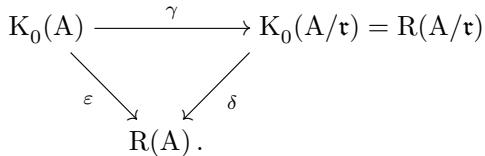
\includegraphics[keepaspectratio]{images/part002_05770a86.jpg}}

我们用 \(\mathcal{S}\) 表示单 A-模的类所成之（有限）集；对每个 \(\lambda \in \mathcal{S}\)，选取一个模 \(S_{\lambda}\)（其类为 \(\lambda\)）和一个投射覆盖 \((P_{\lambda}, u_{\lambda})\)（它覆盖 \(S_{\lambda}\)）（VIII, 第 175 页，命题 4）。由 VIII, 第 176 页的命题 6 得出，\(K_0(A)\) 是一个自由 \(\mathbf{Z}\)-模，以族 \(([P_{\lambda}]_{\mathcal{P}(A)})_{\lambda \in \mathcal{S}}\) 为基。此外，由于 \(S_{\lambda}\) 同构于 \(P_{\lambda} / \mathfrak{r}P_{\lambda}\)（VIII, 第 176 页），\(\gamma\) 把基 \(([P_{\lambda}]_{\mathcal{P}(A)})_{\lambda \in \mathcal{S}}\)（\(K_0(A)\) 的基）变为基 \(([S_{\lambda}])_{\lambda \in \mathcal{S}}\)（\(R(A / \mathfrak{r})\) 的基）。同构 \(\delta\) 把基 \(([S_{\lambda}])_{\lambda \in \mathcal{S}}\)（\(R(A / \mathfrak{r})\) 的基）变为基 \(([S_{\lambda}])_{\lambda \in \mathcal{S}}\)（\(R(A)\) 的基）。

A 的嘉当矩阵是矩阵 \((a_{\lambda\mu})\)，即 Z-模同态 \(\varepsilon: K_{0}(A) \to R(A)\) 关于基 \(([P_{\lambda}]_{\mathcal{P}(A)})_{\lambda \in \mathcal{S}}\)（\(K_{0}(A)\) 的基）与基 \(([S_{\lambda}])_{\lambda \in \mathcal{S}}\)（\(R(A)\) 的基）的矩阵。按定义，我们有

\[
[ \mathrm{P} _ {\mu} ] = \sum_ {\lambda \in \mathcal {S}} a _ {\lambda \mu} [ \mathrm{S} _ {\lambda} ] \quad (\mu \in \mathcal {S})\tag{19}
\]

（在群 R(A) 中）。换句话说，\(a_{\lambda\mu}\) 是同构于 \(S_{\lambda}\) 的商在 A-模 \(P_{\mu}\) 的某条若尔当–赫尔德列中的个数。

令 \(\pi = \varepsilon \circ \gamma^{-1} \circ \delta^{-1}\)；它是群 R(A) 的一个自同态。若 M 是一个有限生成半单 A-模且 (P, \(u\)) 是 M 的一个投射覆盖，则我们有 \(\pi([M]) = [P]\)。由公式 (19)，\(\pi\) 关于 R(A) 的基 \(([S_{\lambda}])_{\lambda \in \mathcal{S}}\) 的矩阵正是 A 的嘉当矩阵。

\subsection{\texorpdfstring{\(K_{0}(A)\) 的换环}{K\_\{0\}(A) 的换环}}

设 A 与 B 是环。设 \(f: A \to B\) 是一个环同态。若 P 是一个有限生成投射 A-模，则 B-模 \(f^{*}(P) = B \otimes_{A} P\) 是投射且有限生成的（II, §5, No.~2, 第 281 页，推论）。映射 \(P \mapsto \text{cl}(f^{*}(P))\) 是从幺半群 \(\mathcal{P}(A)\) 到幺半群 \(\mathcal{P}(B)\) 的一个同态，因此定义了一个同态 \(f^{*}: K_{0}(A) \to K_{0}(B)\)，它由关系式 \(f^{*}([P]_{\mathcal{P}(A)}) = [f^{*}(P)]_{\mathcal{P}(B)}\)（对每个有限生成投射 A-模 P）刻画。若 \(g: B \to C\) 是第二个环同态，则由标量扩张的递移性（II, §5, No.~1, 第 278 页，命题 2）得出，同态 \((g \circ f)^*\) 与 \(g^{*} \circ f^{*}\)（都是从 \(\mathrm{K}_{0}(\mathrm{A})\) 到 \(\mathrm{K}_{0}(\mathrm{C})\) 的同态）相等。

假设 \(f\) 使 B 成为一个有限生成投射左 A-模。设 Q 是一个有限生成投射左 B-模。则 Q 是一个有限生成自由 B-模的直因子，而后者作为 A-模是投射且有限生成的。于是，由 Q 经标量限制得到的 A-模 \(f_{*}(\mathrm{Q})\) 是投射且有限生成的。同上，我们导出一个同态 \(f_{*}: \mathrm{K}_{0}(\mathrm{B}) \to \mathrm{K}_{0}(\mathrm{A})\)，它由关系式 \(f_{*}([Q]_{\mathcal{P}(B)}) = [f_{*}(Q)]_{\mathcal{P}(A)}\)（对每个有限生成投射 B-模 Q）刻画。若 \(g: \mathrm{B} \to \mathrm{C}\) 是使 C 成为有限生成投射 B-模的环同态，则同态 \((g \circ f)_{*}\) 与 \(f_{*} \circ g_{*}\)（都是从 \(\mathrm{K}_{0}(\mathrm{C})\) 到 \(\mathrm{K}_{0}(\mathrm{A})\) 的同态）相等。

\subsection{弗罗贝尼乌斯互反律}

设 A 是一个半单环。设 f 是从 A 到半单环 B 的一个同态。设 S 是一个单 A-模，T 是一个单 B-模，且设 D 与 E 分别是 S 与 T 的中心化子。由舒尔引理（VIII, 第 47 页，推论），D 与 E 都是体。用 H 表示从 S 到 \(f_{*}(\mathrm{T})\) 的 A-线性同态所成之集。我们赋予 H 一个 (E,D)-双模结构，其外部合成律为 \((e,u)\mapsto e\circ u\) 与 \((d,u)\mapsto u\circ d\)（对 \(e\in E\)，\(u\in H\)，\(d\in D\)）。

命题 11. —— a) 重数 \([f_{*}(\mathrm{T}):\mathrm{S}]\)（单 A-模 S 在半单 A-模 \(f_{*}(\mathrm{T})\) 中的重数）等于把 H 视为 D 上右向量空间时的维数。

\begin{enumerate}
\def\labelenumi{\alph{enumi})}
\setcounter{enumi}{1}
\tightlist
\item
  重数 \([f^{*}(\mathrm{S}):\mathrm{T}]\) 是有限的，且等于把 H 视为 E 上左向量空间时的维数。
\end{enumerate}

断言 a) 由 VIII, 第 72 页的公式 (11) 得出。

B-模 \(f^{*}(S)\) 是半单且有限生成的，故具有有限长度。由同前所引的公式 (12)，我们有

\[
[ f ^ {*} (\mathrm{S}): \mathrm{T} ] = \dim_ {\mathrm{E}} \operatorname{Hom} _ {\mathrm{B}} (f ^ {*} (\mathrm{S}), \mathrm{T}).\tag{20}
\]

另外，在 II, §5, No.~1, 第 277--278 页的公式 (2) 与注 2 中，我们定义了一个从 \(\mathrm{Hom}_{\mathrm{A}}(\mathrm{S},f_{*}(\mathrm{T}))\) 到 \(\mathrm{Hom}_{\mathrm{B}}(f^{*}(\mathrm{S}),\mathrm{T})\) 的 E-线性双射。于是断言 b) 由公式 (20) 得出。

推论（弗罗贝尼乌斯互反律）. —— 假设 A 与 B 是交换域 K 上为有限维的半单代数，且 f 是 K-线性的。则 K-向量空间 S、T、D、E 与 H 都是有限维的，并且我们有等式

\[
[ f _ {*} (\mathrm{T}): \mathrm{S} ] [ \mathrm{D}: \mathrm{K} ] = [ f ^ {*} (\mathrm{S}): \mathrm{T} ] [ \mathrm{E}: \mathrm{K} ] = [ \mathrm{H}: \mathrm{K} ].\tag{21}
\]

特别地，当 K 是代数闭的时，我们有 D = E = K，且

\[
[ f _ {*} (\mathrm{T}): \mathrm{S} ] = [ f ^ {*} (\mathrm{S}): \mathrm{T} ] = [ \mathrm{H}: \mathrm{K} ].\tag{22}
\]

由于 A-模 S 是单的，它是单生成的，且 D 是 \(\operatorname{Hom}_{\mathrm{K}}(\mathrm{S},\mathrm{S})\) 的一个线性子空间；故 S 与 D 在 K 上都是有限维的。出于同样的理由，T 与 E 在 K 上是有限维的。最后，H 是 \(\operatorname{Hom}_{\mathrm{K}}(\mathrm{S},\mathrm{T})\) 的一个线性子空间；因而它也是有限维的。于是公式 (21) 由命题 11 得出，因为 H 在 K 上的维数等于 \([H:D][D:K]\)，也等于 \([H:E][E:K]\)（II, §1, No.~13, 第 222 页，命题 25）。由 VIII, 第 47 页的定理 1，若 K 是代数闭的，我们有 D = E = K。于是推论的第二部分由第一部分得出。

设 \(\mathrm{A}\) 与 \(\mathrm{B}\) 是交换域 \(\mathrm{K}\) 上为有限维的半单代数，且设 \(f\) 是一个 \(\mathrm{K}\)-代数同态（从 \(\mathrm{A}\) 到 \(\mathrm{B}\)）。

用 \(\mathcal{S}(\mathrm{A})\) 表示单 A-模的类所成之集；对每个 \(\lambda \in \mathcal{S}(\mathrm{A})\)，设 \(\mathrm{S}_{\lambda}\) 是类为 \(\lambda\) 的一个模，\(\mathrm{D}_{\lambda}\) 是它的中心化子。则 \(\mathrm{D}_{\lambda}\) 是 \(\mathrm{K}\) 上的一个有限次数代数；我们把这个次数记作 \(d_{\lambda}\)。我们类似地定义 \(\mathcal{S}(\mathrm{B})\)、\(\mathrm{T}_{\mu}\)、\(\mathrm{E}_{\mu}\) 与 \(e_{\mu}\)（对 \(\mu\) 属于 \(\mathcal{S}(\mathrm{B})\)）。格罗滕迪克群 \(\mathrm{K}_0(\mathrm{A})\) 以族 \(([\mathrm{S}_{\lambda}])_{\lambda \in \mathcal{S}(\mathrm{A})}\) 为基，而 \(\mathrm{K}_0(\mathrm{B})\) 以族 \(([\mathrm{T}_{\mu}])_{\mu \in \mathcal{S}(\mathrm{B})}\) 为基。设 \((a_{\mu \lambda})\) 是 \(f^{*}: \mathrm{K}_{0}(\mathrm{A}) \to \mathrm{K}_{0}(\mathrm{B})\) 关于这些基的矩阵，\((b_{\lambda \mu})\) 是 \(f_{*}: \mathrm{K}_{0}(\mathrm{B}) \to \mathrm{K}_{0}(\mathrm{A})\) 关于这些基的矩阵。按定义，我们有

\[
a _ {\mu \lambda} = [ f ^ {*} (\mathrm{S} _ {\lambda}): \mathrm{T} _ {\mu} ], \qquad b _ {\lambda \mu} = [ f _ {*} (\mathrm{T} _ {\mu}): \mathrm{S} _ {\lambda} ]\tag{23}
\]

（\(\lambda\) 属于 \(\mathcal{S}(\mathrm{A})\)，\(\mu\) 属于 \(\mathcal{S}(\mathrm{B})\)）。我们把向量空间 \(\mathrm{Hom}_{\mathrm{A}}(\mathrm{S}_{\lambda}, f_{*}(\mathrm{T}_{\mu}))\) 在域 K 上的维数记作 \(h_{\lambda \mu}\)。由上面的推论，我们有

\[
h _ {\lambda \mu} = e _ {\mu} a _ {\mu \lambda} = d _ {\lambda} b _ {\lambda \mu}.\tag{24}
\]

当域 K 是代数闭的时，我们有 \(d_{\lambda} = e_{\mu} = 1\)；于是，我们有

\[
a _ {\mu \lambda} = b _ {\lambda \mu} = h _ {\lambda \mu}.\tag{25}
\]

换句话说，\(f_{*}\) 与 \(f^{*}\) 关于 \(\mathrm{K}_0(\mathrm{A})\) 与 \(\mathrm{K}_0(\mathrm{B})\) 的给定基的矩阵互为转置。

\subsection{单环的情形}

设 A 与 B 是单环，f 是从 A 到 B 的一个同态。设 S 是一个单 A-模，T 是一个单 B-模。我们令

\[
i (f) = [ f ^ {*} (\mathrm{S}): \mathrm{T} ] = \mathrm{long} _ {\mathrm{B}} (f ^ {*} (\mathrm{S}));\tag{26}
\]

我们把基数 \(i(f)\) 称为 f 的指数。当 A 是 B 的子环且 f 是 A 到 B 中的典范单射时，我们把 \(i(\mathrm{B},\mathrm{A})\) 记作 \(i(f)\) 的替代，并把这个基数称为 A 在 B 中的指数。我们类似地定义 f 的高度 \(h(f)\)：

\[
h (f) = [ f _ {*} (\mathrm{T}): \mathrm{S} ] = \mathrm{long} _ {\mathrm{A}} (f _ {*} (\mathrm{T})).\tag{27}
\]

当 A 是 B 的子环且 f 是 A 到 B 中的典范单射时，我们用 \(h(\mathrm{B}, \mathrm{A})\) 表示 \(h(f)\)，并把它称为 A 在 B 中的高度。

A-模 S 是单生成的，故 B-模 \(f^{*}(\mathrm{S}) = \mathrm{B} \otimes_{\mathrm{A}} \mathrm{S}\) 亦然。由此得出 \(i(f)\) 是有限的，从而是一个整数。设 M 是一个 A-模。用 a 表示它的长度；则 M 同构于 \(\mathrm{S}^{(\mathfrak{a})}\)。于是 B-模 \(f_{*}(\mathrm{M})\) 同构于 \(f_{*}(\mathrm{S})^{(\mathfrak{a})}\)。由 \(i(f)\) 的定义，我们因此有

\[
\mathrm{long} _ {\mathrm{B}} (f ^ {*} (\mathrm{M})) = i (f) \mathrm{long} _ {\mathrm{A}} (\mathrm{M}).\tag{28}
\]

Z-模 \(K_{0}(A)\) 与 \(K_{0}(B)\) 都是维数为 1 的自由模，分别以 {[}S{]} 与 {[}T{]} 为基，并且我们有

\[
f ^ {*} ([ \mathrm{S} ]) = i (f) [ \mathrm{T} ].\tag{29}
\]

特别地，取 \(M = A_{s}\)；则 \(f^{*}(A_{s}) = B \otimes_{A} A_{s}\) 同构于 \(B_{s}\)（II, §3, No.~4, 第 249 页），故

\[
i (f) = \mathrm{long(B)} / \mathrm{long(A)}.\tag{30}
\]

由韦德伯恩定理（VIII, 第 120 页，定理 1），存在整数 \(m \geqslant 1\) 与 \(n \geqslant 1\) 以及体 D 与 E，使得 A 同构于 \(\mathbf{M}_m(\mathrm{D})\)，B 同构于 \(\mathbf{M}_n(\mathrm{E})\)。由公式 (30)，我们有 \(i(f) = n / m\)；特别地，\(m\) 整除 \(n\)。

设 N 是一个 B-模；用 a 表示它的长度。则 N 同构于 \(\mathrm{T}^{(\mathfrak{a})}\)，故 A-模 \(f_{*}(\mathrm{N})\) 同构于 \(f_{*}(\mathrm{T})^{(\mathfrak{a})}\)；由 \(h(f)\) 的定义，我们有

\[
\mathrm{long} _ {\mathrm{A}} (f _ {*} (\mathrm{N})) = h (f) \mathrm{long} _ {\mathrm{B}} (\mathrm{N}).\tag{31}
\]

我们已经看到（VIII, 第 124 页，命题 5），f 使 B 成为一个自由 A-模，且该模的所有基都具有同一基数，记作 \([B:A]_{s}\)，称为 B 在 A 上的（左）次数。A-模 \(f_{*}(B_{s})\) 同构于 \(A_{s}^{[B:A]_{s}}\)，故其长度为 \([B:A]_{s}\) long(A)。把公式 (30) 与公式 (31) 应用于特例 \(N=B_{s}\)，我们因此有

\[
[ \mathrm{B}: \mathrm{A} ] _ {s} = i (f) h (f).\tag{32}
\]

现在假设 B 是一个有限生成 A-模，即 \([B:A]_{s}\) 是有限的。则由公式 (32)，\(h(f)\) 是有限的。我们（在 VIII, 第 202 页）定义了一个群同态 \(f_{*}\)（从 \(K_{0}(B)\) 到 \(K_{0}(A)\)）；我们有

\[
f _ {*} ([ \mathrm{T} ]) = h (f) [ \mathrm{S} ].\tag{33}
\]

假设 A 与 B 是交换域 K 上为有限维的代数，且 f 是 K-线性的。同前，存在整数 \(m \geqslant 1\) 与 \(n \geqslant 1\)、为体的 K-代数 D 与 E，以及从 A 到 \(\mathbf{M}_{m}(\mathrm{D})\)、从 B 到 \(\mathbf{M}_{n}(\mathrm{E})\) 的 K-代数同构。令 \(d = [D : K]\) 且 \(e = [E : K]\)。我们于是有关系式

\[
[ \mathrm{A}: \mathrm{K} ] = m ^ {2} d, \qquad [ \mathrm{B}: \mathrm{K} ] = n ^ {2} e, \qquad [ \mathrm{B}: \mathrm{A} ] _ {s} = \frac {n ^ {2} e}{m ^ {2} d}
\]

以及，由公式 (30) 与 (32)，关系式

\[
i (f) = \frac {n}{m}, \qquad h (f) = \frac {n e}{m d}.
\]

当域 \(\mathrm{K}\) 是代数闭的时，我们有 \(d = e = 1\)，因此 \(i(f) = h(f)\) 且 \([\mathrm{B}:\mathrm{A}]_s = i(f)^2\)。

设 A、B 与 C 是单环，且设 \(f: A \to B\) 与 \(g: B \to C\) 是同态。设 S 是一个单 A-模。C-模 \((g \circ f)^{*}(S)\) 与 \(g^{*}(f^{*}(S))\) 同构；因此，由公式 (26) 与 (28)，我们有

\[
i (g \circ f) = \operatorname{long} _ {\mathrm{C}} \left(g ^ {*} \left(f ^ {*} (\mathrm{S})\right)\right) = i (g) \operatorname{long} _ {\mathrm{B}} \left(f ^ {*} (\mathrm{S})\right) = i (g) i (f).
\]

我们可以类似地证明等式 \(h(g \circ f) = h(g)h(f)\)。当 A 是 B 的子环且 B 是 C 的子环，并且对 f 与 g 取典范单射时，这些等式给出

\[
i (\mathrm{C}, \mathrm{A}) = i (\mathrm{C}, \mathrm{B}) i (\mathrm{B}, \mathrm{A}), \qquad h (\mathrm{C}, \mathrm{A}) = h (\mathrm{C}, \mathrm{B}) h (\mathrm{B}, \mathrm{A}).\tag{34}
\]

命题 12. —— 设 B 是一个单环，A 是 B 的一个单子环。假设 B 是一个有限生成左 A-模。设 M 是一个非零的有限生成左 B-模。令 \(A' = \text{End}_{A}(M)\) 且 \(B' = \text{End}_{B}(M)\)。则 \(B'\) 是 \(A'\) 的一个子环，环 \(A'\) 与 \(B'\) 都是单的，\(A'\) 是一个有限生成左 \(B'\)-模，并且我们有等式

\[
i (\mathrm{A} ^ {\prime}, \mathrm{B} ^ {\prime}) = h (\mathrm{B}, \mathrm{A}), \quad h (\mathrm{A} ^ {\prime}, \mathrm{B} ^ {\prime}) = i (\mathrm{B}, \mathrm{A}), \quad [ \mathrm{A} ^ {\prime}: \mathrm{B} ^ {\prime} ] _ {s} = [ \mathrm{B}: \mathrm{A} ] _ {s}.
\]

由 VIII, 第 123 页的命题 4，环 \(\mathrm{A}'\) 是单的，\(\mathrm{M}\) 是一个有限长度的 \(\mathrm{A}'\)-模，并且我们有

\[
\mathrm{long} _ {\mathrm{A}} (\mathrm{M}) = \mathrm{long} (\mathrm{A} ^ {\prime}), \quad \mathrm{long} _ {\mathrm{A} ^ {\prime}} (\mathrm{M}) = \mathrm{long} (\mathrm{A}).
\]

出于同样的理由，环 \(B'\) 是单的，并且我们有

\[
\operatorname{long} _ {\mathrm{B}} (\mathrm{M}) = \operatorname{long} \left(\mathrm{B} ^ {\prime}\right), \quad \operatorname{long} _ {\mathrm{B} ^ {\prime}} (\mathrm{M}) = \operatorname{long} (\mathrm{B}).
\]

于是，由公式 (31) 与 (30)，我们有

\[
h (\mathrm{B}, \mathrm{A}) = \operatorname{long} _ {\mathrm{A}} (\mathrm{M}) / \operatorname{long} _ {\mathrm{B}} (\mathrm{M}) = \operatorname{long} \left(\mathrm{A} ^ {\prime}\right) / \operatorname{long} \left(\mathrm{B} ^ {\prime}\right) = i \left(\mathrm{A} ^ {\prime}, \mathrm{B} ^ {\prime}\right);
\]

等式 \(h(\mathrm{A}^{\prime},\mathrm{B}^{\prime}) = i(\mathrm{B},\mathrm{A})\) 可以类似地建立。由此我们导出

\[
[ \mathrm{A} ^ {\prime}: \mathrm{B} ^ {\prime} ] _ {s} = i (\mathrm{A} ^ {\prime}, \mathrm{B} ^ {\prime}) h (\mathrm{A} ^ {\prime}, \mathrm{B} ^ {\prime}) = h (\mathrm{B}, \mathrm{A}) i (\mathrm{B}, \mathrm{A}) = [ \mathrm{B}: \mathrm{A} ] _ {s}
\]

（利用公式 (32)）。特别地，\(A'\) 是一个有限生成左 \(B'\)-模。

\BourbakiExercises{习题}

\begin{enumerate}
\def\labelenumi{\arabic{enumi})}
\tightlist
\item
  设 p 是一个素数。用 C 表示形如 \((\mathbf{Z}/p^{2}\mathbf{Z})^{n} \oplus (\mathbf{Z}/p^{3}\mathbf{Z})^{m}\)（\(n, m \in N\)）的 Z-模的类所成之集。
\end{enumerate}

\begin{enumerate}
\def\labelenumi{\alph{enumi})}
\item
  证明 \(\mathcal{C}\) 是加性的但不是遗传的。最小的遗传集 \(\mathcal{H}\)（它包含 \(\mathcal{C}\)）是什么？
\item
  证明 C 型模的每个短正合列都分裂。描述群 \(\mathrm{K}(\mathcal{C})\)。
\item
  构造一个正合列
\end{enumerate}

\[
0 \to \mathrm{M} _ {0} \to \mathrm{M} _ {1} \to \mathrm{M} _ {2} \to \mathrm{M} _ {3} \to \mathrm{M} _ {4} \to 0
\]

（由 C 型模组成），使得 \(M_{0} \oplus M_{2} \oplus M_{4}\) 与 \(M_{1} \oplus M_{3}\) 在 \(\mathrm{K}(\mathcal{C})\) 中的类不相同。

\begin{enumerate}
\def\labelenumi{\alph{enumi})}
\setcounter{enumi}{3}
\tightlist
\item
  从 \(\mathrm{K}(\mathcal{C})\) 到 \(\mathrm{K}(\mathcal{H})\) 的自然同态是否是单射？
\end{enumerate}

\begin{enumerate}
\def\labelenumi{\arabic{enumi})}
\setcounter{enumi}{1}
\item
  设 \(\mathrm{A}\) 是一个环，\(a\) 与 \(b\) 是 \(\mathrm{A}\) 中满足 \(ab = 1\) 与 \(ba \neq 1\) 的两个元素。证明 A-模 \(\mathrm{A}(1 - ba)\) 是投射的，并且它与零 A-模稳定同构。更精确地说，证明 A-模 \(\mathrm{A}_s\) 与 \(\mathrm{A}(1 - ba) \oplus \mathrm{A}_s\) 同构。
\item
  设 A 与 B 是环。用 A 与 B 的格罗滕迪克群确定格罗滕迪克群 \(R(A \times B)\) 与 \(K_{0}(A \times B)\)（都是 \(A \times B\) 的）。
\item
  设 A 与 B 是森田等价的环。证明群 R(A) 与 R(B) 同构。对 \(K_{0}(A)\) 与 \(K_{0}(B)\) 同样处理。
\item
  设 A 是一个环。用 \(\mathcal{I}(A)\) 表示由偶 \((n,p)\)（其中 n 是整数，p 是 \(M_{n}(A)\) 中的一个幂等元）组成的集。在 \(\mathcal{I}(A)\) 上定义一个加法：令 \((m,p)+(n,q)=(m+n,\begin{pmatrix} p & 0 \\ 0 & q \end{pmatrix})\)。
\end{enumerate}

\begin{enumerate}
\def\labelenumi{\alph{enumi})}
\item
  设 \(\mathcal{P}(A^{\circ})\) 是有限生成投射右 A-模的类所成的幺半群。设 \(\varphi: \mathcal{I}(A) \to \mathcal{P}(A^{\circ})\) 是由 \(\varphi(n,p) = \operatorname{cl}(\operatorname{Im}p)\) 定义的映射。证明 \(\varphi\) 是一个满同态，且元素 \((m,p)\) 与 \((n,q)\)（都属于 \(\mathcal{I}(A)\)）在 \(\varphi\) 下有相同的像当且仅当存在 \(a \in M_{m,n}(A)\) 与 \(b \in M_{n,m}(A)\)，使得 ab = p 且 ba = q。
\item
  由此推出群 \(K_{0}(A)\) 与 \(K_{0}(A^{\circ})\) 同构。
\end{enumerate}

\begin{enumerate}
\def\labelenumi{\arabic{enumi})}
\setcounter{enumi}{5}
\tightlist
\item
  设 A 是一个环，G 是一个交换群，T: A → G 是一个迹型映射（VIII, 第 115 页，习题 3）。对每个有限生成投射右 A-模 P，用
\end{enumerate}

\[
\mathrm{T} _ {\mathrm{P}}: \operatorname{End} _ {\mathrm{A}} (\mathrm{P} \oplus \mathrm{A} _ {d}) \longrightarrow \mathrm{G}
\]

表示扩张 T 的唯一迹型映射（同前所引），并用 \(\pi_{P}\) 表示 \(\operatorname{End}_{\mathrm{A}}(\mathrm{P} \oplus \mathrm{A}_{d})\) 中以 P 为像、以 \(A_{d}\) 为核的投影子。构造一个群同态 \(\widetilde{\mathrm{T}} : \mathrm{K}_{0}(\mathrm{A}) \to \mathrm{G}\)，使得对每个有限生成投射右 A-模 P，有 \(\widetilde{\mathrm{T}}([\mathrm{P}]) = \mathrm{T}_{\mathrm{P}}(\pi_{\mathrm{P}})\)。

\begin{enumerate}
\def\labelenumi{\arabic{enumi})}
\setcounter{enumi}{6}
\tightlist
\item
  设 I 是一个右有向集，\((\mathrm{A}_{i}, f_{ji})\) 是环的一个直接系统，A 是它的极限。证明 \(\mathrm{K}_{0}(\mathrm{A})\) 是群的直接系统 \((\mathrm{K}_{0}(\mathrm{A}_{i}), f_{ji}^{*})\) 的极限。
\end{enumerate}

¶ 8) 设 A、B 与 C 是环，\(f: \mathrm{A} \to \mathrm{C}\) 与 \(g: \mathrm{B} \to \mathrm{C}\) 是环同态；假设 \(f\) 是满射。考虑 \(\mathrm{A} \times \mathrm{B}\) 中由偶 \((a, b)\)（满足 \(f(a) = g(b)\)）组成的子环 D。设 M 是一个 A-模，N 是一个 B-模，\(u\) 是从 \(\mathrm{C} \otimes_{\mathrm{A}} \mathrm{M}\) 到 \(\mathrm{C} \otimes_{\mathrm{B}} \mathrm{N}\) 的一个 C-同构。用 P 表示 \(\mathrm{M} \times \mathrm{N}\) 中由偶 \((m, n)\)（满足 \(u(1 \otimes m) = 1 \otimes n\)）组成的 D-子模。

\begin{enumerate}
\def\labelenumi{\alph{enumi})}
\item
  假设模 M 与 N 分别具有有限基 \((e_{i})_{i\in\mathrm{I}}\) 与 \((f_{j})_{j\in\mathrm{J}}\)，并且 u 在基 \((1\otimes e_{i})\) 与 \((1\otimes f_{j})\) 下的矩阵是一个以 A 为元素的逆矩阵 \((a_{ji})\) 的像。证明 D-模 P 是自由的；更精确地说，元素 \((e_{i},\sum_{j}a_{ji}f_{j})_{i\in\mathrm{I}}\) 构成 P 的一个基。
\item
  设 p 与 q 是整数，\(X \in \mathbf{M}_{p,q}(\mathrm{C})\) 与 \(Y \in \mathbf{M}_{q,p}(\mathrm{C})\) 是满足 \(XY = I_{p}\) 与 \(YX = I_{q}\) 的矩阵。证明方阵 \(\begin{pmatrix} X & 0 \\ 0 & Y \end{pmatrix}\) 是某个以 A 为元素的逆矩阵的像，利用恒等式
\end{enumerate}

\[
\left( \begin{array}{c c} X & 0 \\ 0 & Y \end{array} \right) = \left( \begin{array}{c c} I _ {p} & X \\ 0 & I _ {q} \end{array} \right) \left( \begin{array}{c c} I _ {p} & 0 \\ - Y & I _ {q} \end{array} \right) \left( \begin{array}{c c} I _ {p} & X \\ 0 & I _ {q} \end{array} \right) \left( \begin{array}{c c} 0 & - I _ {p} \\ I _ {q} & 0 \end{array} \right).
\]

\begin{enumerate}
\def\labelenumi{\alph{enumi})}
\setcounter{enumi}{2}
\item
  假设模 M 与 N 是自由且有限生成的。由 a) 与 b) 推出 D-模 P 是投射且有限生成的。
\item
  假设 M 与 N 是投射且有限生成的。构造一个 A-模 \(M'\) 与一个 B-模 \(N'\)，使得 \(M \oplus M'\) 与 \(N \oplus N'\) 是自由且有限生成的，并且 C-模 \(C \otimes_{A} M'\) 与 \(C \otimes_{B} N'\) 同构。由此推出 D-模 P 是投射且有限生成的。
\item
  证明由两个投射导出的典范同态 \(A \otimes_{D} P \to M\) 与 \(B \otimes_{D} P \to N\) 是双射（如上那样化归为 a) 的条件成立的情形）。
\item
  反之，设 \(P'\) 是一个有限生成投射 D-模；令 \(M' = A \otimes_{D} P'\) 与 \(N' = B \otimes_{D} P'\)，并用 \(u' : C \otimes_{A} M' \to C \otimes_{B} N'\) 表示典范同构。证明从 \(P'\) 到 \(M' \times N'\) 的典范同态诱导一个从 \(P'\) 到与 \((M', N', u')\) 相伴的 D-模上的 D-线性同构。
\end{enumerate}

\(g)\) 用 \(\varphi_0:\mathrm{K}_0(\mathrm{D})\to \mathrm{K}_0(\mathrm{A})\times \mathrm{K}_0(\mathrm{B})\) 与 \(\psi_0:\mathrm{K}_0(\mathrm{A})\times \mathrm{K}_0(\mathrm{B})\to \mathrm{K}_0(\mathrm{C})\) 表示满足

\[
\varphi_ {0} ([ \mathrm{P} ]) = ([ \mathrm{A} \otimes_ {\mathrm{D}} \mathrm{P} ], [ \mathrm{B} \otimes_ {\mathrm{D}} \mathrm{P} ]) \quad \text { and } \quad \psi_ {0} ([ \mathrm{M} ], [ \mathrm{N} ]) = [ \mathrm{C} \otimes_ {\mathrm{A}} \mathrm{M} ] - [ \mathrm{C} \otimes_ {\mathrm{B}} \mathrm{N} ].
\]

证明序列

\[
\mathrm{K} _ {0} (\mathrm{D}) \xrightarrow {\varphi_ {0}} \mathrm{K} _ {0} (\mathrm{A}) \times \mathrm{K} _ {0} (\mathrm{B}) \xrightarrow {\psi_ {0}} \mathrm{K} _ {0} (\mathrm{C})
\]

是正合的。证明若此外还存在一个环同态 \(s: C \to A\) 使得 \(f \circ s = Id_{C}\)，则 \(\varphi_{0}\) 是单射且 \(\psi_{0}\) 是满射。

\begin{enumerate}
\def\labelenumi{\arabic{enumi})}
\setcounter{enumi}{8}
\tightlist
\item
  设 A 是一个伪环，即一个结合的但不必含单位元的 Z-代数，\(\widetilde{A}\) 是由 A 通过添加单位元（III, §1, No.~2, 第 431 页）得到的 Z-代数；集合 \(\widetilde{\mathrm{A}}\) 等于 \(\mathbf{Z} \times \mathrm{A}\)。把同态 \((n, a) \mapsto n\) 记作 \(\varepsilon : \widetilde{\mathrm{A}} \to \mathbf{Z}\)，并把同态 \(\varepsilon^{*} : \mathrm{K}_{0}(\widetilde{\mathrm{A}}) \to \mathrm{K}_{0}(\mathbf{Z})\)（它与 \(\varepsilon\) 相伴）的核记作 \(\mathrm{K}_{0}(\mathrm{A})\)。
\end{enumerate}

\begin{enumerate}
\def\labelenumi{\alph{enumi})}
\item
  证明若 A 含单位元，则 \(\tilde{A}\) 同构于积环 \(Z \times A\)，且 \(K_{0}(A)\) 的这一定义与 No.~8 中给出的定义相容。
\item
  设 A 与 B 是伪环，\(f: \mathrm{A} \to \mathrm{B}\) 是一个同态。设 \(\widetilde{f}: \widetilde{\mathrm{A}} \to \widetilde{\mathrm{B}}\) 是由 \(\widetilde{f}((n, a)) = (n, f(a))\) 定义的环同态。证明 \(\widetilde{f}^*\) 把 \(\mathrm{K}_0(\mathrm{A})\) 映到 \(\mathrm{K}_0(\mathrm{B})\) 之中。把由 \(\widetilde{f}^*\) 导出的同态记作 \(f^*: \mathrm{K}_0(\mathrm{A}) \to \mathrm{K}_0(\mathrm{B})\)。c) 假设 \(f\) 是满射；用 \(\mathfrak{a}\) 表示它的核，并把 \(\mathfrak{a}\) 到 A 中的典范单射记作 \(i\)。证明序列
\end{enumerate}

\[
\mathrm{K} _ {0} (\mathfrak {a}) \xrightarrow {i ^ {*}} \mathrm{K} _ {0} (\mathrm{A}) \xrightarrow {f ^ {*}} \mathrm{K} _ {0} (\mathrm{B})
\]

是正合的。若此外还存在伪环的同态 \(s: B \to A\) 使得 \(f \circ s = Id_{B}\)，则 \(i^{*}\) 是单射且 \(f^{*}\) 是满射（对三元组 (A, B, C) 先取 (A, A, B) 再取 (D, Z, A)，应用习题 8）。

\begin{enumerate}
\def\labelenumi{\alph{enumi})}
\setcounter{enumi}{3}
\tightlist
\item
  证明习题 7 与 8 的结论可推广到伪环的情形。e) 用 \(\mathbf{M}_{\infty}(\mathrm{A})\) 表示以 A 为元素且仅有有限多个非零元素的 \(\mathbf{N} \times \mathbf{N}\) 矩阵所成的伪环。设 \(f: \mathrm{A} \to \mathbf{M}_{\infty}(\mathrm{A})\) 是把 \(a \in \mathrm{A}\) 映到矩阵 \((b_{ij})\)（满足 \(b_{00} = a\) 与 \(b_{ij} = 0\)，当 \((i,j) \neq (0,0)\)）的映射。证明 \(f^{*}\) 是从 \(\mathrm{K}_0(\mathrm{A})\) 到 \(\mathrm{K}_0(\mathbf{M}_{\infty}(\mathrm{A}))\) 的同构（利用习题 4 与 7）。
\end{enumerate}

\begin{enumerate}
\def\labelenumi{\arabic{enumi})}
\setcounter{enumi}{9}
\tightlist
\item
  设 A 是一个环。用 \(\mathbf{GL}_{\infty}(\mathrm{A})\) 表示 \(\mathbf{GL}(\mathrm{A}^{(\mathbf{N})})\) 中由满足 X - I 仅有有限多个非零元素的矩阵 X 组成的子群，并用 \(\mathrm{E}(\mathrm{A})\) 表示 \(\mathbf{GL}_{\infty}(\mathrm{A})\) 中由形如 \(I + \lambda E_{ij}\)（其中 i, j 属于 N，\(i \neq j\)，\(\lambda \in A\)）的矩阵生成的子群；它是 \(\mathbf{GL}_{\infty}(\mathrm{A})\) 的导群（II, §10, 第 422 页，习题 15）。把商群 \(\mathbf{GL}_{\infty}(\mathrm{A}) / \mathrm{E}(\mathrm{A})\) 记作 \(\mathrm{K}_{1}(\mathrm{A})\)；它的群运算写作加法。每个环同态 \(f : A \to B\) 诱导一个群同态 \(f^{*} : K_{1}(A) \to K_{1}(B)\)。
\end{enumerate}

\begin{enumerate}
\def\labelenumi{\alph{enumi})}
\item
  对每个整数 \(n \geqslant 1\)，设 \(\iota_{n} : \mathbf{GL}_{n}(\mathrm{A}) \to \mathrm{K}_{1}(\mathrm{A})\) 是把 \(X \in \mathbf{GL}_{n}(\mathrm{A})\) 映到矩阵 \(\begin{pmatrix} X & 0 \\ 0 & I \end{pmatrix}\) 的类的同态。证明若环 A 是局部环，则对每个 n，\(\iota_{n}\) 是满射（利用 VIII, 第 42 页，习题 17）。
\item
  假设环 A 是交换的。构造一个满同态 \(d_{\mathrm{A}} : \mathrm{K}_{1}(\mathrm{A}) \to \mathrm{A}^{*}\)，使得对每个 n 有 \(d_{A} \circ \iota_{n} = det\)。若此外 A 是局部环或欧几里得环，则同态 \(d_{A}\) 与 \(\iota_{1}\) 是互逆的双射。
\item
  设 I 是一个右有向集，\((\mathrm{A}_{i}, f_{ji})\) 是环的一个直接系统，A 是它的极限。证明 \(\mathrm{K}_{1}(\mathrm{A})\) 是群的直接系统 \((\mathrm{K}_{1}(\mathrm{A}_{i}), f_{ji}^{*})\) 的极限。
\end{enumerate}

¶ 11) 采用习题 8 的假设与记号。用 \(f': \mathrm{D} \to \mathrm{B}\) 与 \(g': \mathrm{D} \to \mathrm{A}\) 表示由两个投射导出的同态，并用

\[
\varphi_ {1}: \mathrm{K} _ {1} (\mathrm{D}) \rightarrow \mathrm{K} _ {1} (\mathrm{A}) \times \mathrm{K} _ {1} (\mathrm{B}) \quad \text { and } \quad \psi_ {1}: \mathrm{K} _ {1} (\mathrm{A}) \times \mathrm{K} _ {1} (\mathrm{B}) \rightarrow \mathrm{K} _ {1} (\mathrm{C})
\]

表示由 \(\varphi_1(z) = (g'^* (z), f'^* (z))\) 与 \(\psi_1(x,y) = f^* (x) - g^* (y)\) 定义的映射。

\begin{enumerate}
\def\labelenumi{\alph{enumi})}
\tightlist
\item
  证明序列
\end{enumerate}

\[
\mathrm{K} _ {1} (\mathrm{D}) \xrightarrow {\varphi_ {1}} \mathrm{K} _ {1} (\mathrm{A}) \times \mathrm{K} _ {1} (\mathrm{B}) \xrightarrow {\psi_ {1}} \mathrm{K} _ {1} (\mathrm{C})
\]

是正合的（注意 \(f(\mathrm{E}(\mathrm{A})) = \mathrm{E}(\mathrm{C})\)）。证明若此外还存在一个环同态 \(s : C \to A\) 使得 \(f \circ s = Id_{C}\)，则 \(\psi_{1}\) 是满射。

\begin{enumerate}
\def\labelenumi{\alph{enumi})}
\setcounter{enumi}{1}
\item
  对每个整数 n 与 \(\mathbf{GL}_{n}(\mathrm{C})\) 的每个元素 g，用 \(P_{g}\) 表示与模 \(A^{n}\)、\(B^{n}\) 以及从 \(C \otimes_{A} A^{n}\) 到 \(C \otimes_{B} B^{n}\) 的以 g 为矩阵的同构相伴的投射 D-模（习题 8）。构造一个同态 \(\partial : K_{1}(\mathrm{C}) \to K_{0}(\mathrm{D})\)，使得 \(\partial \circ \iota_{n}(g) = [\mathrm{P}_{g}] - [\mathrm{D}_{s}^{n}]\) 对每个整数 n 与 \(\mathbf{GL}_{n}(\mathrm{C})\) 的每个元素 g 成立。
\item
  证明序列
\end{enumerate}

\[
\mathrm{K} _ {1} (\mathrm{D}) \xrightarrow {\varphi_ {1}} \mathrm{K} _ {1} (\mathrm{A}) \times \mathrm{K} _ {1} (\mathrm{B}) \xrightarrow {\psi_ {1}} \mathrm{K} _ {1} (\mathrm{C}) \xrightarrow {\partial} \mathrm{K} _ {0} (\mathrm{D}) \xrightarrow {\varphi_ {0}} \mathrm{K} _ {0} (\mathrm{A}) \times \mathrm{K} _ {0} (\mathrm{B}) \xrightarrow {\psi_ {0}} \mathrm{K} _ {0} (\mathrm{C})
\]

是正合的。

\begin{enumerate}
\def\labelenumi{\arabic{enumi})}
\setcounter{enumi}{11}
\tightlist
\item
  设 \(f: \mathrm{A} \to \mathrm{B}\) 是一个满射环同态，\(\mathfrak{a}\) 是其核，且 \(i\) 是从 \(\mathfrak{a}\) 到 \(\mathrm{A}\) 的典范单射。构造一个同态 \(\partial: \mathrm{K}_1(\mathrm{B}) \to \mathrm{K}_0(\mathfrak{a})\)，使得序列
\end{enumerate}

\[
\mathrm{K} _ {1} (\mathrm{A}) \xrightarrow {f ^ {*}} \mathrm{K} _ {1} (\mathrm{B}) \xrightarrow {\partial} \mathrm{K} _ {0} (\mathfrak {a}) \xrightarrow {i ^ {*}} \mathrm{K} _ {0} (\mathrm{A}) \xrightarrow {f ^ {*}} \mathrm{K} _ {0} (\mathrm{B})
\]

是正合的（按习题 11, c) 的方式论证）。

\begin{enumerate}
\def\labelenumi{\arabic{enumi})}
\setcounter{enumi}{12}
\item
  用 \(\mathcal{C}\)（相应地，\(\mathcal{D}\)）表示有限长度 \(\mathbf{Z}\)-模（相应地，有限生成 \(\mathbf{Z}\)-模）的类所成之集。证明群同态 \(\gamma_{\mathcal{D},\mathcal{C}}\)（从 \(\mathrm{K}(\mathcal{C})\) 到 \(\mathrm{K}(\mathcal{D})\)）是零同态。
\item
  设 K 是一个特征异于 2 的交换域。令
\end{enumerate}

\[
\mathrm{A} = \mathrm{K} [ \mathrm{X}, \mathrm{Y}, \mathrm{Z} ] / (\mathrm{X} ^ {2} + \mathrm{Y} ^ {2} + \mathrm{Z} ^ {2} - 1).
\]

设 M 是 A-模 \(\mathrm{A}^{3}/\mathrm{A}(\overline{\mathrm{X}},\overline{\mathrm{Y}},\overline{\mathrm{Z}})\)，其中 \(\overline{X}\)、\(\overline{Y}\) 与 \(\overline{Z}\) 分别表示 X、Y 与 Z 在 A 中的像。证明 \(M\oplus A\) 是自由 A-模，但 M 不是自由模。

\section{半单模的张量积}

在本节中，字母 K 表示一个交换域。若 E 与 F 是 K 上的向量空间，则我们把张量积 \(E \otimes_{K} F\) 记作 \(E \otimes F\)。

\subsection{代数的张量积上的半单模}

在本小节中，我们考虑 K-代数 \(A_{1}\) 与 \(A_{2}\)；我们把代数 \(A_{1} \otimes A_{2}\) 记作 A。

命题 1. —— 设 \(M_{1}\) 是一个 \(A_{1}\)-模，\(M_{2}\) 是一个 \(A_{2}\)-模，二者都不约化为 0。若模 \(M = M_{1} \otimes M_{2}\)（环 \(A = A_{1} \otimes A_{2}\) 上的模）是单模（相应地，同构模、半单模），则 \(A_{1}\)-模 \(M_{1}\) 与 \(A_{2}\)-模 \(M_{2}\) 是单模（相应地，同构模、半单模）。

假设 M 是半单 A-模。设 \(N_{1}\) 是一个 \(A_{1}\)-子模（\(M_{1}\) 的）。用 N 表示 \(N_{1} \otimes M_{2}\) 在 A-模 M 中的典范像。由 VIII, 第 56 页，推论 2，存在 M 中一个以 N 为像的 A-线性投影子 p。由假设，\(M_{2} \neq 0\)；因此可以选取 \(M_{2}\) 的一个元素 m 和一个线性形式 \(\varphi\)（在 K-向量空间 \(M_{2}\) 上，满足 \(\varphi(m) = 1\)）（II, §7, No.~5, 第 302 页，推论 2）。设 u 是从 \(M_{1}\) 到 M 的映射，由 \(u(m_{1}) = m_{1} \otimes m\) 定义；v 是从 M 到 \(M_{1}\) 的 K-线性映射，由 \(v(m_{1} \otimes m_{2}) = \varphi(m_{2})m_{1}\) 刻画。令 \(q = v \circ p \circ u\)。映射 \(q : M_{1} \to M_{1}\) 是 \(A_{1}\)-线性的，它的像含于 \(N_{1}\)，并且我们有 \(q(n) = n\)（对每个 \(n \in N_{1}\)）。于是，q 是 \(M_{1}\) 中以 \(N_{1}\) 为像的投影子。我们证明了 \(M_{1}\) 是半单 \(A_{1}\)-模（VIII, 第 56 页，推论 2）。

假设 M 是单模，且 \(M_{1}\) 是两个 \(A_{1}\)-子模 \(M_{1}^{\prime}\) 与 \(M_{1}^{\prime\prime}\) 的直和。令 \(M^{\prime}=M_{1}^{\prime}\otimes M_{2}\) 与 \(M^{\prime\prime}=M_{1}^{\prime\prime}\otimes M_{2}\)；则 M 是 A-子模 \(M'\) 与 \(M''\) 的直和。由于 M 是单模，\(M'\) 或 \(M''\) 必约化为 0；由假设 \(M_{2} \neq 0\)，故 \(M_{1}' = 0\) 或 \(M_{1}'' = 0\)（II, §3, No.~7, 第 256 页，推论 2）。这就证明了 \(M_{1}\) 是单 \(A_{1}\)-模。

现在假设 M 是同构 A-模。设 S 与 T 是两个单 \(A_{1}\)-子模（属于 \(M_{1}\)）。于是 A-模 \(S \otimes M_{2}\) 与 \(T \otimes M_{2}\) 可与 M 的非零子模视为同一。因而它们是与 M 同型的同构模。由注 VIII, 第 61 页，存在一个非零 A-线性映射 \(f : S \otimes M_{2} \to T \otimes M_{2}\)。映射 f 特别还是 \(A_{1}\)-线性的。由于 \(A_{1}\)-模 \(S \otimes M_{2}\) 与 \(T \otimes M_{2}\) 非零，且分别是 S 型与 T 型的同构模，故 S 与 T 同构。这就证明了 \(M_{1}\) 是同构 \(A_{1}\)-模。

命题 2. —— 设 S 是环 \(A = A_{1} \otimes A_{2}\) 上的一个单模，在 K 上有限维。对 \(i \in \{1, 2\}\)，存在一个单 \(A_{i}\)-模 \(S_{i}\)，使得 \(A_{i}\)-模 S 是 \(S_{i}\) 型的同构模。A-模 S 同构于 A-模 \(S_{1} \otimes S_{2}\) 的一个商。

由于 S 是一个在 K 上有限维的非零 \(A_{1}\)-模，它在 \(A_{1}\) 上有有限长度，且存在一个单左 \(A_{1}\)-模 \(S_{1}\) 以及一个非零 \(A_{1}\)-线性映射（从 \(S_{1}\) 到 S）。我们赋予 \(\mathrm{M}_{2} = \mathrm{Hom}_{\mathrm{A}_{1}}(\mathrm{S}_{1}, \mathrm{S})\) 一个左 \(A_{2}\)-模结构，它由外合成律 \((a_{2}, u) \mapsto (a_{2})_{\mathrm{S}} \circ u\) 定义。由构造，\(M_{2} \neq 0\)，且 \(M_{2}\) 在 K 上有限维。因此可以找到一个单左 \(A_{2}\)-模 \(S_{2}\) 与一个非零 \(A_{2}\)-线性映射 \(\varphi : S_{2} \to M_{2}\)。我们定义一个非零 A-线性映射 \(\psi\)（从 \(S_{1} \otimes S_{2}\) 到 S），由

\[
\psi (s _ {1} \otimes s _ {2}) = \varphi (s _ {2}) (s _ {1})\tag{1}
\]

（对每个 \(s_{1} \in S_{1}\) 与 \(s_{2} \in S_{2}\)）。由于 S 是单 A-模且 \(\psi\) 非零，\(\psi\) 是满射，从而 S 同构于 \(S_{1} \otimes S_{2}\) 的一个商。对 \(i \in \{1, 2\}\)，\(A_{i}\)-模 \(S_{1} \otimes S_{2}\) 是 \(S_{i}\) 型的同构模，因此 \(A_{i}\)-模 S 亦然（VIII, 第 61 页，命题 2）。

对任意 K-代数 B，我们用 \(\mathcal{S}_{\mathrm{K}}(\mathrm{B})\) 表示在 K 上有限维的单（VIII, 第 51 页）左 B-模的类所成之集。

定理 1. —— 假设体 K 是代数封闭的。

\begin{enumerate}
\def\labelenumi{\alph{enumi})}
\item
  设 \(M_{1}\) 是一个 \(A_{1}\)-模，\(M_{2}\) 是一个 \(A_{2}\)-模，二者都是在 K 上有限维的单模（相应地，半单模）。则 \(M_{1} \otimes M_{2}\) 是环 \(A_{1} \otimes A_{2}\) 上的单模（相应地，半单模），且在 K 上有限维。
\item
  从 \(\mathcal{S}_{\mathrm{K}}(\mathrm{A}_1)\times \mathcal{S}_{\mathrm{K}}(\mathrm{A}_2)\) 到 \(\mathcal{S}_{\mathrm{K}}(\mathrm{A}_1\otimes \mathrm{A}_2)\) 的、把 \((\operatorname {cl}(\mathrm{S}_1),\operatorname {cl}(\mathrm{S}_2))\) 映到 \(\operatorname {cl}(\mathrm{S}_1\otimes \mathrm{S}_2)\) 的映射（其中 \(\mathrm{S}_1\)（相应地，\(\mathrm{S}_2\)）是单 \(\mathrm{A}_1\)-模（相应地，单 \(\mathrm{A}_2\)-模），且在 \(\mathrm{K}\) 上有限维）是双射。
\end{enumerate}

为证明 a)，只需考虑 \(M_{1}\) 与 \(M_{2}\) 都是单模的情形。设 \(M'\) 是 \(M = M_{1} \otimes M_{2}\) 的一个 A-子模；它是一个 \(A_{1}\)-子模（属于 \(M_{1} \otimes M_{2}\)），在形如 \(1_{M_{1}} \otimes u\)（其中 u 取遍 \(A_{2}\)-模 \(M_{2}\) 的位似所成之集）的自同态集下稳定。由于体 K 是代数封闭的，舒尔引理（VIII, 第 47 页，定理 1）蕴含交换子 \(\operatorname{End}_{\mathrm{A}_{1}}(\mathrm{M}_{1})\)（即 \(M_{1}\) 的交换子）等于 K。由 VIII, 第 63 页，推论 2，A-子模 \(M'\)（\(M_{1} \otimes M_{2}\) 的）形如 \(M_{1} \otimes M_{2}'\)，其中 \(M_{2}'\) 是一个 \(A_{2}\)-子模（\(M_{2}\) 的）。我们已假设 \(M_{2}\) 是单模；因此 \(M_{2}' = 0\) 或 \(M_{2}' = M_{2}\)，即 \(M' = 0\) 或 \(M' = M\)。于是，M 是单模。

若 S 是 \(A_{1} \otimes A_{2}\) 上在 K 上有限维的单模，则由命题 2 与 a) 可知，S 同构于形如 \(S_{1} \otimes S_{2}\) 的模，其中 \(S_{1}\)（相应地，\(S_{2}\)）是单 \(A_{1}\)-模（相应地，单 \(A_{2}\)-模）。此外，作为 \(A_{i}\)-模，S 是 \(S_{i}\) 型的同构模，故 \(S_{i}\) 的类只依赖于 S 的类。这就证明了 b)。

注. —— 1) 当不假设体 K 代数封闭时，定理 1 的断言 a) 不再成立。可以举出这样的例子（VIII, 第 225 页，习题 4）：\(M_{i}\) 是在 K 上有限维的单 \(A_{i}\)-模（对 \(i \in \{1, 2\}\)），而 A-模 \(M_{1} \otimes M_{2}\) 不是半单的，或者是半单的但不是单的。

\begin{enumerate}
\def\labelenumi{\arabic{enumi})}
\setcounter{enumi}{1}
\tightlist
\item
  存在一个同态 \(\varphi\)（从 \(\mathrm{R_K(A_1)\otimes_{\mathbf{Z}} R_K(A_2)}\) 到 \(\mathrm{R_K(A)}\)），由关系式 \(\varphi ([\mathrm{M}_1]\otimes [\mathrm{M}_2]) = [\mathrm{M}_1\otimes \mathrm{M}_2]\) 刻画。这可以用与 VIII, 第 196 页，命题 9 相同的方式证明。若体 \(K\) 是代数封闭的，则由定理 1, b)，\(\varphi\) 是从 \(\mathrm{R_K(A_1)\otimes_{\mathbf{Z}} R_K(A_2)}\) 到 \(\mathrm{R_K(A)}\) 的同构，因为对每个 K-代数 B，\(\mathbf{Z}\)-模 \(\mathrm{R_K(B)}\) 是自由的，以族 \(([\mathrm{S}])_{\mathrm{S}\in \mathcal{S}_{\mathrm{K}}(\mathrm{B})}\) 为基（VIII, 第 195 页）。
\end{enumerate}

\subsection{单模的张量积}

设 \(A_{1}\) 与 \(A_{2}\) 是交换域 K 上的代数。我们把 K-代数 \(A_{1} \otimes A_{2}\) 记作 A。

引理 1. —— 设 \(M_{1}\) 与 \(N_{1}\) 是 \(A_{1}\)-模，\(M_{2}\) 与 \(N_{2}\) 是 \(A_{2}\)-模。我们作如下假设：

\begin{enumerate}
\def\labelenumi{(\roman{enumi})}
\item
  \(A_{1}\)-模 \(M_{1}\) 是有限生成的。
\item
  \(A_{2}\)-模 \(M_{2}\) 是有限生成的，或者 \(N_{1}\) 在 K 上有限维。
\end{enumerate}

令 \(\mathrm{M} = \mathrm{M}_1\otimes \mathrm{M}_2\) 与 \(\mathrm{N} = \mathrm{N}_1\otimes \mathrm{N}_2\)，并把它们视为环 \(\mathrm{A} = \mathrm{A}_1\otimes \mathrm{A}_2\) 上的模。典范同态（II, §3, No.~5, 第 251 页）

\[
\lambda : \operatorname{Hom} _ {\mathrm{K}} (\mathrm{M} _ {1}, \mathrm{N} _ {1}) \otimes \operatorname{Hom} _ {\mathrm{K}} (\mathrm{M} _ {2}, \mathrm{N} _ {2}) \longrightarrow \operatorname{Hom} _ {\mathrm{K}} (\mathrm{M}, \mathrm{N})
\]

于是诱导 K-向量空间的一个同构

\[
\varphi : \operatorname{Hom} _ {\mathrm{A} _ {1}} (\mathrm{M} _ {1}, \mathrm{N} _ {1}) \otimes \operatorname{Hom} _ {\mathrm{A} _ {2}} (\mathrm{M} _ {2}, \mathrm{N} _ {2}) \longrightarrow \operatorname{Hom} _ {\mathrm{A}} (\mathrm{M}, \mathrm{N}).
\]

映射 \(\lambda\) 是单射（II, §7, No.~7, 第 308 页，命题 16），并把线性子空间 \(\mathrm{Hom}_{\mathrm{A}_1}(\mathrm{M}_1,\mathrm{N}_1)\otimes \mathrm{Hom}_{\mathrm{A}_2}(\mathrm{M}_2,\mathrm{N}_2)\) 映到 \(\mathrm{Hom}_{\mathrm{A}}(\mathrm{M},\mathrm{N})\)。因此只需证明每个从 M 到 N 的 A-线性映射都属于 \(\mathrm{Hom}_{\mathrm{A}_1}(\mathrm{M}_1,\mathrm{N}_1)\otimes \mathrm{Hom}_{\mathrm{A}_2}(\mathrm{M}_2,\mathrm{N}_2)\) 在 \(\lambda\) 下的像。设 \(u:\mathrm{M}\to \mathrm{N}\) 是一个 A-线性映射。设 \(x\in \mathrm{M}_1\)。用 \(u_{x}\) 表示 \(\mathrm{A}_2\)-线性映射 \(y\mapsto u(x\otimes y)\)（从 \(\mathrm{M}_2\) 到 \(\mathrm{N}_1\otimes \mathrm{N}_2\)）。令 \(\mathrm{P} = \mathrm{Hom}_{\mathrm{A}_2}(\mathrm{M}_2,\mathrm{N}_2)\)，并用 \(\nu\) 表示从 \(\mathrm{N}_1\otimes \mathrm{P}\) 到 \(\mathrm{Hom}_{\mathrm{A}_2}(\mathrm{M}_2,\mathrm{N}_1\otimes \mathrm{N}_2)\) 的典范同态（II, §4, No.~2, 第 269 页）。这个映射是单射（II, §4, No.~2, 第 269 页，命题 2, (i)，应用于 K-向量空间 \(\mathbf{N}_1\)）。由假设 (ii)，存在一个线性子空间 \(\mathrm{V}_x\)（\(\mathbf{N}_1\) 的，在 K 上有限维），使得 \(u_{x}\) 取值于 \(\mathrm{V}_x\otimes \mathrm{N}_2\)。由此可知，\(u_{x}\) 是 \(\nu\) 下某个唯一元素 \(v_{x}\)（属于 \(\mathbf{N}_1\otimes \mathbf{P}\)）的像。映射 \(\widetilde{u}:x\mapsto v_x\)（从 \(\mathbf{M}_1\) 到 \(\mathbf{N}_1\otimes \mathbf{P}\)）是 \(\mathbf{A}_1\)-线性的。由假设 (i)，\(\mathbf{A}_1\)-模 \(\mathbf{M}_1\) 是有限生成的。与上面类似的论证表明，\(\widetilde{u}\) 属于 \(\mathrm{Hom}_{\mathrm{A}_1}(\mathrm{M}_1,\mathrm{N}_1)\otimes \mathrm{P}\) 在 \(\mathrm{Hom}_{\mathrm{A}_1}(\mathrm{M}_1,\mathrm{N}_1\otimes \mathrm{P})\) 中的像。引理 1 得证。

定理 2. —— 设 \(A_{1}\) 与 \(A_{2}\) 是交换域 K 上的代数；设 \(S_{1}\) 是单 \(A_{1}\)-模，\(S_{2}\) 是单 \(A_{2}\)-模。设 \(D_{1}\) 与 \(D_{2}\) 分别是 \(S_{1}\) 与 \(S_{2}\) 的交换子。令 \(M = S_{1} \otimes S_{2}\)，\(A = A_{1} \otimes A_{2}\)，\(D = D_{1} \otimes D_{2}\)。我们把 M 视为左 (A,D)-双模。

\begin{enumerate}
\def\labelenumi{\alph{enumi})}
\item
  A-模 M 的交换子等于 \(\mathrm{D}_{\mathrm{M}}\)。
\item
  映射 \(a \mapsto aM\) 是从按包含关系排序的 D 的右理想所成之集到按包含关系排序的 M 的 A-子模所成之集的同构。逆映射把 M 的子模 N 映到由满足 \(dM \subset N\) 的元素 d 组成的 D 的理想。
\end{enumerate}

断言 a) 由引理 1 得出，因为单模是单生成的。

设 \(\mathrm{T}\) 是 \((\mathrm{A}_1, \mathrm{D}_2)\)-双模 \(\mathrm{S}_1 \otimes (\mathrm{D}_2)_d\)。我们把 \(\mathrm{M} = \mathrm{S}_1 \otimes \mathrm{S}_2\) 与 \(\mathrm{T} \otimes_{\mathrm{D}_2} \mathrm{S}_2\) 视为同一（II, §3, No.~8, 第 258 页）；这一视为同一与环 \(\mathrm{A} = \mathrm{A}_1 \otimes \mathrm{A}_2\) 上的左模结构相容。

设 \(\mathrm{N}\) 是 \(\mathrm{M}\) 的一个 A-子模；它是 \(\mathrm{A}_2\)-子模（属于 \(\mathrm{T} \otimes_{\mathrm{D}_2} \mathrm{S}_2\)），在形如 \((a_1)_\mathrm{T} \otimes 1_{\mathrm{S}_2}\)（其中 \(a_1\) 取遍 \(\mathrm{A}_1\)）的自同态下稳定。由 VIII, 第 63 页，推论 2，存在唯一的 \((\mathrm{A}_1, \mathrm{D}_2)\)-子双模 \(\mathrm{V}\)（\(\mathrm{T}\) 的），使得 \(\mathrm{N} = \mathrm{V} \otimes_{\mathrm{D}_2} \mathrm{S}_2\)。

同构 \(u\)（从 \(\mathrm{T} = \mathrm{S}_1 \otimes (\mathrm{D}_2)_d\) 到 \(((\mathrm{D}_1)_d \otimes (\mathrm{D}_2)_d) \otimes_{\mathrm{D}_1} \mathrm{S}_1\)，由 \(u(s \otimes d) = 1 \otimes d \otimes s\) 定义）是 \((\mathrm{A}_1, \mathrm{D}_2)\)-线性的。我们把这些 \((\mathrm{A}_1, \mathrm{D}_2)\)-双模视为同一。与上面给出的论证类似，可以证明存在唯一的右 \((\mathrm{D}_1 \otimes \mathrm{D}_2)\)-子模 \(\mathfrak{a}\)（\(\mathrm{D}_1 \otimes \mathrm{D}_2\) 的），使得 \(\mathrm{V} = \mathfrak{a} \otimes_{\mathrm{D}_1} \mathrm{S}_1\)。考虑到上面所作的视为同一，\(\mathfrak{a}\) 是 \(\mathrm{D} = \mathrm{D}_1 \otimes \mathrm{D}_2\) 的唯一使得 \(\mathrm{N} = \mathfrak{a}\mathrm{M}\) 的右理想。

我们刚刚证明了映射 \(a \mapsto aM\) 是双射；最后的断言由此得出。

推论 1. —— 模 \(S_{1} \otimes S_{2}\)（环 \(A_{1} \otimes A_{2}\) 上的）是半单的（相应地，同型的、单的）当且仅当环 \(D = D_{1} \otimes D_{2}\) 是半单的（相应地，单环、体）。特别地，\(S_{1} \otimes S_{2}\) 是单模（当 \(S_{1}\) 或 \(S_{2}\) 的交换子等于 K 时）。

由定理 2，模 \(S_{1} \otimes S_{2}\)（环 \(D_{1} \otimes D_{2}\) 上的）是半单的（相应地，同型的、单的）当且仅当右 D-模 \((\mathrm{D}_{1} \otimes \mathrm{D}_{2})_{d}\) 是（VIII, 第 109 页，命题 10）。而右 D-模 \(D_{d}\) 是单模当且仅当 D 是体；它是同型的（相应地，半单的）当且仅当环 D 是单环（相应地，半单环）（VIII, 第 120 页，定义 1；VIII, 第 121 页，推论 1；以及 VIII, 第 137 页，命题 2）。

推论 2. —— 我们有 \(\mathfrak{R}_{\mathrm{A}}(\mathrm{M}) = \mathfrak{R}(\mathrm{D})\mathrm{M}\)。A-模 M 无根当且仅当环 D 无根。

这由 VIII, 第 108 页，命题 8 与定理 2, b) 得出。

\subsection{半单交换代数的张量积}

定理 3. —— 设 \(\mathbf{Z}_1\) 与 \(\mathbf{Z}_2\) 是 \(\mathbf{K}\) 上的半单交换代数。环 \(\mathbf{Z}_1 \otimes \mathbf{Z}_2\) 的根等于它的幂零元素所成之集。

我们先处理 \(Z_{1}\) 与 \(Z_{2}\) 是体 K 的扩张 \(L_{1}\) 与 \(L_{2}\) 的情形。必要时交换 \(L_{1}\) 与 \(L_{2}\)，可化归为 \(L_{1}\) 在 K 上的超越次数小于 \(L_{2}\) 在 K 上的超越次数的情形。

选取一个代数闭包 \(\Omega\)（\(\mathrm{L}_2\) 的）；由 V, §14, No.~6, 第 114 页，定理 5 的推论 1，我们可以假设 \(\mathrm{L}_1\) 是 \(\Omega\) 的一个子扩张。

\begin{enumerate}
\def\labelenumi{\Alph{enumi})}
\item
  我们先证明 \(L_{1} \otimes L_{2}\) 的根含于 \(L_{1} \otimes \Omega\) 的根。令 \(\mathfrak{a} = \Re(L_{1} \otimes L_{2})(L_{1} \otimes \Omega)\)；它是交换环 \(L_{1} \otimes \Omega\) 的一个理想，我们必须证明 a 含于 \(L_{1} \otimes \Omega\) 的根。换句话说（VIII, 第 156 页，定理 1），我们必须证明对 \(x \in a\)，元素 \(1 + x\) 在 \(L_{1} \otimes \Omega\) 中可逆。由于 \(\Omega\) 是 \(L_{2}\) 的代数扩张，存在一个有限次数的扩张 \(L_{3}\)（\(L_{2}\) 的），使得 x 属于 \(\Re(L_{1} \otimes L_{2})(L_{1} \otimes L_{3})\)。显然只需证明 \(1 + x\) 在 \(L_{1} \otimes L_{3}\) 中可逆。而 \(C = L_{1} \otimes L_{3}\) 是环 \(B = L_{1} \otimes L_{2}\) 上的一个有限生成模。由 VIII, 第 175 页的推论，我们有 \(\Re(B)C \subset \Re(C)\)，故 x 属于 C 的根，从而 \(1 + x\) 在 C 中可逆。
\item
  我们来证明 \(L_{1} \otimes \Omega\) 的根由幂零元素组成。用 p 表示 K 的特征指数，用 P 表示 K 在 \(\Omega\) 中的相对 p-根式（即纯不可分）闭包（V, §5, No.~2, 第 25 页）；体 P 是完备的。由于 P 是 K 的代数扩张，我们有 \(\mathrm{L}_{1}(\mathrm{P}) = \mathrm{L}_{1}[\mathrm{P}]\)（V, §3, No.~2, 第 18 页，推论 1）。设 b 是从 \(L_{1} \otimes P\) 到体 \(P_{1} = L_{1}[P]\) 的典范同态的核。设 \(x \in b\)；存在元素 \(y_{1}, \ldots, y_{n}\)（\(L_{1}\) 的）与元素 \(z_{1}, \ldots, z_{n}\)（P 的），使得 \(x = \sum_{i=1}^{n} y_{i} \otimes z_{i}\) 且 \(\sum_{i=1}^{n} y_{i} z_{i} = 0\)。由于 P 在 K 上是 p-根式的，存在 p 的一个幂 q，使得 \(z_{1}^{q}, \ldots, z_{n}^{q}\) 属于 K。于是我们有
\end{enumerate}

\[
x ^ {q} = \sum_ {i = 1} ^ {n} y _ {i} ^ {q} \otimes z _ {i} ^ {q} = \sum_ {i = 1} ^ {n} y _ {i} ^ {q} z _ {i} ^ {q} \otimes 1 = \left(\sum_ {i = 1} ^ {n} y _ {i} z _ {i}\right) ^ {q} \otimes 1 = 0.
\]

所以 b 由幂零元素组成。

令 \(c = b \otimes_{P} \Omega\)；它是从 \((\mathrm{L}_{1} \otimes \mathrm{P}) \otimes_{\mathrm{P}} \Omega\) 到 \(P_{1} \otimes_{P} \Omega\) 的典范同态的核，且由上面的论证知它由幂零元素组成。而 \(\Omega\) 是 P 的代数封闭扩张，\(P_{1}\) 是 \(\Omega\) 的一个子扩张。由于体 P 是完备的，\(P_{1}\) 是 P 的可分扩张（V, §15, No.~5, 第 125 页，定理 3）。由 V, 第 120 页，定理 4，交换环 \(P_{1} \otimes_{P} \Omega\) 的诸极大理想之交约化为 0。换句话说，环 \(P_{1} \otimes_{P} \Omega\)（它同构于 \(((L_{1} \otimes P) \otimes_{P} \Omega)/c\)）是无根的。这就证明（VIII, 第 155 页，命题 5）c 包含环 \((\mathrm{L}_{1} \otimes \mathrm{P}) \otimes_{\mathrm{P}} \Omega\) 的根。而这一环同构于 \(L_{1} \otimes \Omega\)，且 c 由幂零元素组成。因此，\(L_{1} \otimes \Omega\) 的根由幂零元素组成。

\begin{enumerate}
\def\labelenumi{\Alph{enumi})}
\setcounter{enumi}{2}
\tightlist
\item
  特殊情形证明的结尾。由 A) 与 B)，根 \(\mathfrak{r}\)（\(\mathrm{L}_1\otimes \mathrm{L}_2\) 的）含于这一交换环的幂零元素所成之集 \(\mathfrak{n}\)。此外我们知道 \(\mathfrak{n}\) 含于 \(\mathfrak{r}\)（VIII, 第 157 页，注 2）。
\end{enumerate}

现在考虑一般情形。由于半单交换 K-代数是体 K 的有限多个扩张的积（VIII, 第 137 页，命题 3），且环的积的根是诸根的积（VIII, 第 156 页，推论 3），\(Z_{1} \otimes Z_{2}\) 的根是这一环的幂零元素所成之集。

\subsection{代数的张量积的根}

设 \(A_{1}\) 与 \(A_{2}\) 是 K-代数，令 \(A = A_{1} \otimes A_{2}\)。

命题 3. —— 假设代数 \(\mathrm{A}_1\) 与 \(\mathrm{A}_2\) 是半单的，其中心分别为 \(\mathbf{Z}_1\) 与 \(\mathbf{Z}_2\)。令 \(\mathbf{Z} = \mathbf{Z}_1 \otimes \mathbf{Z}_2\)。

\begin{enumerate}
\def\labelenumi{\alph{enumi})}
\item
  映射 \(a \mapsto aA\) 是从按包含关系排序的 Z 的理想所成之集到按包含关系排序的 A 的双边理想所成之集的同构。
\item
  A 的根等于 A 的诸极大双边理想之交，且等于 \(\Re(Z)A\)。
\item
  若 K-代数 \(Z_{1}\) 与 \(Z_{2}\) 之一是可分的，特别地若体 K 是完备的，则环 Z 与 A 的根均约化为 0。
\end{enumerate}

每个代数 \(A_{i}\) 都是有限多个单代数的积。而环的积的中心是诸中心的积，且对根（VIII, 第 156 页，推论 3）与对双边理想（I, §8, No.~10, 第 109 页，命题 8）也有类似的断言。因此只需在 \(A_{1}\) 与 \(A_{2}\) 都是单代数的假设下证明命题 3。

对 \(i \in \{1,2\}\)，令 \(B_i = A_i \otimes A_i^o\)，并把 \(A_i\) 视为一个 \(B_i\)-模，其中位似由公式

\[
(x \otimes y) z = x z y
\]

给出，其中 x、y 与 z 属于 \(A_{i}\)。\(B_{i}\)-模 \(A_{i}\) 的交换子是 \((\mathrm{Z}_{i})_{\mathrm{A}_{i}}\)，即由 \(Z_{i}\) 的元素作的位似所成之集；我们把它与 \(Z_{i}\) 视为同一。此外，\(B_{i}\)-子模（\(A_{i}\) 的）就是 \(A_{i}\) 的双边理想，且由于环 \(A_{i}\) 是单环，仅有的双边理想是 0 与 \(A_{i}\)。因而 \(A_{i}\) 是单 \(B_{i}\)-模。再者，\((\mathrm{B}_{1}\otimes\mathrm{B}_{2})\)-子模（\(A_{1}\otimes A_{2}\) 的）就是环 \(A_{1}\otimes A_{2}\) 的双边理想。

于是，把 VIII, 第 214 页，定理 2, b) 应用于单 \(\mathrm{B}_1\)-模 \(\mathrm{A}_1\)（交换子为 \(\mathrm{Z}_1\)）以及单 \(\mathrm{B}_2\)-模 \(\mathrm{A}_2\)（交换子为 \(\mathrm{Z}_2\)），即得断言 a)。

我们来证明断言 b)。A 的诸极大双边理想之交是 \((\mathrm{B}_{1}\otimes\mathrm{B}_{2})\)-模 \(A_{1}\otimes A_{2}\) 的根；由 VIII, 第 215 页，推论 2，这一交与 \(\Re(\mathrm{Z})\mathrm{A}\) 重合。代数 \(Z_{1}\) 与 \(Z_{2}\) 是交换且半单的。因此环 Z 的根由幂零元素组成（VIII, 第 215 页，定理 3），且环 A 的双边理想 \(\Re(\mathrm{Z})\mathrm{A}\) 含于根 \(\Re(\mathrm{A})\)（VIII, 第 157 页，注 1）。然而，A 的诸极大双边理想之交包含 \(\Re(\mathrm{A})\)（VIII, 第 155 页，命题 5, d)）。这就证明了断言 b)。

可分交换代数与既约交换代数的张量积是既约环（V, §15, No.~2, 第 120 页，命题 5）。代数 \(Z_1\) 与 \(Z_2\) 是交换且半单的，因而是既约的。若代数 \(Z_1\) 与 \(Z_2\) 之一是可分的，则代数 \(Z\) 是既约的；于是由 VIII, 第 215 页，定理 3，它是无根的，且我们有 \(\Re(A) = \Re(Z)A = 0\)。特别地，当体 \(K\) 完备时即属此种情形，因为完备体上的每个既约交换代数都是可分的（V, §15, No.~5, 第 125 页，定理 3）。

推论. —— 假设代数 \(A_{1}\) 与 \(A_{2}\) 都是单的，且中心 \(Z_{1}\)（\(A_{1}\) 的）约化为 K。则环 \(A_{1} \otimes A_{2}\) 除 0 与其自身外没有其他双边理想。

由假设，\(Z_{1} = K\)，且由于 \(A_{2}\) 是单的，其中心 \(Z_{2}\) 是一个体（VIII, 第 121 页，推论 1, a)）。因此环 \(Z = Z_{1} \otimes Z_{2}\) 是体，推论由命题 3, a) 得出。

\subsection{半单模的张量积}

命题 4. —— 对 \(i \in \{1,2\}\)，设 \(\mathrm{A}_i\) 是一个 K-代数，\(\mathrm{M}_i\) 是一个半单 \(\mathrm{A}_i\)-模，\(\mathrm{Z}_i\) 是 \(\mathrm{M}_i\) 的交换子的中心。令 \(\mathrm{A} = \mathrm{A}_1 \otimes \mathrm{A}_2\)，\(\mathrm{M} = \mathrm{M}_1 \otimes \mathrm{M}_2\)，\(\mathrm{Z} = \mathrm{Z}_1 \otimes \mathrm{Z}_2\)。我们有 \(\Re_{\mathrm{A}}(\mathrm{M}) = \Re(\mathrm{Z})\mathrm{M}\)。若代数 \(\mathrm{Z}_1\) 与 \(\mathrm{Z}_2\) 之一在 \(\mathrm{K}\) 上可分，特别地若体 \(\mathrm{K}\) 是完备的，则 A-模 \(\mathrm{M}\) 无根。

对 \(i \in \{1,2\}\)，设 \(S_i\) 是一个单 \(A_i\)-模，\(D_i\) 是它的交换子，\(I(i)\) 是一个集合。我们先处理 \(M_i\) 是 \(A_i\)-模 \(S_i^{(I(i))}\) 的情形。我们把它的交换子的中心 \(Z_i\) 与 \(D_i\) 的中心视为同一。令 \(D = D_1 \otimes D_2\)。

我们有 \(\Re (\mathrm{D}) = \Re (\mathrm{Z})\mathrm{D}\)（VIII, 第 217 页，命题 3）与 \(\Re_{\mathrm{A}}(\mathrm{S}_1\otimes \mathrm{S}_2) =\) \(\Re (\mathrm{D})(\mathrm{S}_1\otimes \mathrm{S}_2)\)（VIII, 第 215 页，推论 2），因而 \(\Re_{\mathrm{A}}(\mathrm{S}_1\otimes \mathrm{S}_2) = \Re (\mathrm{Z})(\mathrm{S}_1\otimes \mathrm{S}_2)\)。A-模 M 是一族同构于 \(\mathrm{S}_1\otimes \mathrm{S}_2\) 的 A-模的直和，而一族模的直和的根是诸根的直和（VIII, 第 152 页，推论 2）。因此我们有 \(\Re_{\mathrm{A}}(\mathrm{M}) = \Re (\mathrm{Z})\mathrm{M}\)。

现在考虑一般情形。对 \(i \in \{1,2\}\)，把 \(A_{i}\)-模 \(M_{i}\) 的支集记作 \(S_{M_{i}}\)。对 \(\lambda \in S_{M_{i}}\)，把 \(M_{i}\) 的 \(\lambda\) 型同型分量记作 \(M_{i;\lambda}\)，并把它的交换子的中心记作 \(Z_{i;\lambda}\)。我们把环 \(Z_{i}\) 与诸环 \(Z_{i;\lambda}\)（\(\lambda \in S_{M_{i}}\)）的积视为同一。设 \(\lambda \in S_{M_{1}}\) 与 \(\mu \in S_{M_{2}}\)。用 \(i_{\lambda}: Z_{1;\lambda} \to Z_{1}\) 表示唯一的 K-线性映射，使得 \(pr_{\lambda} \circ i_{\lambda}\) 是 \(Z_{1;\lambda}\) 上的恒同映射，且 \(pr_{\lambda'} \circ i_{\lambda}\) 是零映射（对 \(\lambda' \in S_{M_{1}} = \{\lambda\}\)）。同样地定义 \(i_{\mu}: Z_{2;\mu} \to Z_{2}\)。令 \(Z_{\lambda,\mu} = Z_{1;\lambda} \otimes Z_{2;\mu}\) 与 \(i_{\lambda,\mu} = i_{\lambda} \otimes i_{\mu}\)，并把映射 \(pr_{\lambda} \otimes pr_{\mu}\)（从 Z 到 \(Z_{\lambda,\mu}\)）记作 \(\pi_{\lambda,\mu}\)。映射 \(\pi_{\lambda,\mu}\) 是一个满射环同态；因此我们有 \(\pi_{\lambda,\mu}(\Re(Z)) \subset \Re(Z_{\lambda,\mu})\)（VIII, 第 155 页，命题 5, b)）。我们来证明反包含。设 z 是 \(\Re(Z_{\lambda,\mu})\) 的一个元素；由于 \(Z_{1;\lambda}\) 与 \(Z_{2;\mu}\) 都是体，z 是幂零的（VIII, 第 215 页，定理 3）。我们有 \(i_{\lambda,\mu}(xy) = i_{\lambda,\mu}(x) \cdot i_{\lambda,\mu}(y)\)（对 \(Z_{\lambda,\mu}\) 中的 x、y）；因此 \(i_{\lambda,\mu}(z)\) 是幂零的，从而属于 \(\Re(Z)\)。由于 \(\pi_{\lambda,\mu} \circ i_{\lambda,\mu}\) 是 \(Z_{\lambda,\mu}\) 上的恒同映射，元素 z 属于 \(\pi_{\lambda,\mu}(\Re(Z))\)。我们就这样证明了等式 \(\pi_{\lambda,\mu}(\Re(Z)) = \Re(Z_{\lambda,\mu})\)。

令 \(M_{\lambda,\mu}=M_{1;\lambda}\otimes M_{2;\mu}\)；这是 M 的一个在 Z 下稳定的子模。对 \(z\in Z\) 与 \(m\in M_{\lambda,\mu}\)，我们有 \(zm=\pi_{\lambda,\mu}(z)m\)。因此，\(\Re(Z)M_{\lambda,\mu}\) 等于 \(\Re(Z_{\lambda,\mu})M_{\lambda,\mu}\)，从而由同型情形知等于 \(\Re_{A}(M_{\lambda,\mu})\)。由于直和的根是诸根的直和（VIII, 第 152 页，推论 2），且 M 是诸子模 \(M_{\lambda,\mu}\)（\((\lambda,\mu)\in\mathcal{S}_{\mathrm{M}_{1}}\times\mathcal{S}_{\mathrm{M}_{2}}\)）的直和，等式 \(\Re_{A}(M)=\Re(Z)M\) 得证。最后的断言则由 VIII, 第 217 页，命题 3 得出。

引理 2. —— 设 \(A_{1}\) 与 \(A_{2}\) 是交换域 K 上的代数。设 \(M_{1}\) 是一个在 K 上有限维的 \(A_{1}\)-模，\(M_{2}\) 是一个有限长度的 \(A_{2}\)-模。则 \(A_{1} \otimes A_{2}\)-模 \(M_{1} \otimes M_{2}\) 具有有限长度。

令 \(M = M_{1} \otimes M_{2}\)。设 \((e_{1}, \ldots, e_{n})\) 是 \(M_{1}\) 在体 K 上的一个基。映射 \((x_{1}, \ldots, x_{n}) \mapsto \sum_{i=1}^{n} e_{i} \otimes x_{i}\) 是从 \(A_{2}\)-模 \(M_{2}^{n}\) 到 \(A_{2}\)-模 M 的同构。由于 \(M_{2}\) 是有限长度的 \(A_{2}\)-模，M 亦然。此外，M 的每个 A-子模都是 \(A_{2}\)-子模；因此 M 是有限长度的 A-模。

命题 5. —— 设 \(A_{1}\) 与 \(A_{2}\) 是交换域 K 上的代数。设 \(M_{1}\) 是一个在 K 上有限维的半单 \(A_{1}\)-模，\(M_{2}\) 是一个半单 \(A_{2}\)-模。对 \(i \in \{1,2\}\)，把 \(A_{i}\)-模 \(M_{i}\) 的交换子记作 \(D_{i}\)，并把 \(D_{i}\) 的中心记作 \(Z_{i}\)。令 \(A = A_{1} \otimes A_{2}\)，\(M = M_{1} \otimes M_{2}\)，\(D = D_{1} \otimes D_{2}\)，\(Z = Z_{1} \otimes Z_{2}\)。

\begin{enumerate}
\def\labelenumi{\alph{enumi})}
\item
  A-模 M 的交换子可与 D 视为同一，它的中心是 Z。若 \(A_{2}\)-模 \(M_{2}\) 具有有限长度，则 A-模 M 具有有限长度，环 D 是右且左阿廷的，环 Z 是阿廷的。
\item
  下列性质等价：
\end{enumerate}

\begin{enumerate}
\def\labelenumi{(\roman{enumi})}
\item
  A-模 M 是半单的。
\item
  环 \(Z\) 同构于一族交换域的积。
\item
  环 Z 是既约的。
\end{enumerate}

\begin{enumerate}
\def\labelenumi{\alph{enumi})}
\setcounter{enumi}{2}
\tightlist
\item
  下列性质等价：
\end{enumerate}

\begin{enumerate}
\def\labelenumi{(\roman{enumi})}
\item
  A-模 M 是同型的且不约化为 0。
\item
  环 Z 是一个体。
\item
  环 \(\mathbf{Z}\) 是一个整环。
\end{enumerate}

由假设，\(M_{1}\) 在 K 上有限维。因此 M 的交换子可与 D 视为同一（VIII, 第 213 页，引理 1），且它的中心是 Z（III, §4, No.~4, 第 468 页，推论）。假设 \(A_{2}\)-模 \(M_{2}\) 具有有限长度。由引理 2，A-模 M 具有有限长度。由于 \(M_{2}\) 是半单且有限生成的，环 \(D_{2}\) 是半单的（VIII, 第 139 页，命题 6），且它的中心 \(Z_{2}\) 是有限族交换域的积。于是，\(D_{2}\)-模 \((\mathrm{D}_{2})_{s}\) 与 \(Z_{2}\)-模 \((\mathrm{Z}_{2})_{s}\) 都具有有限长度。此外，由于 \(M_{1}\) 在 K 上有限维，\(D_{1}\) 与 \(Z_{1}\) 亦然。由引理 2，模 \((\mathrm{D}_{1} \otimes \mathrm{D}_{2})_{s}\) 具有有限长度；因此环 \(D_{1} \otimes D_{2}\) 是左阿廷的。我们同样可证环 \(D_{1} \otimes D_{2}\) 是右阿廷的，且环 \(Z_{1} \otimes Z_{2}\) 是阿廷的。断言 a) 得证。

我们来证明 b)。半单模的交换子的中心同构于一族交换域的积（VIII, 第 87 页，命题 8, a)）；这就证明了 (i) 蕴含 (ii)。蕴含关系 (ii) \(\Rightarrow\) (iii) 是明显的。

假设环 Z 是既约的。则我们有 \(\Re(Z)=0\)（VIII, 第 215 页，定理 3）与 \(\Re_{\mathrm{A}}(\mathrm{M})=0\)（VIII, 第 218 页，命题 4）。由于 \(A_{2}\)-模 \(M_{2}\) 是半单的，存在一个族 \((\mathrm{S}_{i})_{i\in\mathrm{I}}\)（由单 \(A_{2}\)-模组成）以及一个从 \(M_{2}\) 到 \(\bigoplus S_{i}\) 的同构。因此，A-模 M 同构于 \(\bigoplus M_{1}\otimes S_{i}\)。于是对每个 \(i\in I\)，A-模 \(M_{1}\otimes S_{i}\) 无根。由 a)，它具有有限长度；故它是半单的（VIII, 第 153 页，命题 3, b)）。于是 A-模 M 是一族半单模的直和，从而是半单的。这就证明了 (iii) 蕴含 (i)，并完成了 b) 的证明。

一个 A-模是同型的且非零的，当且仅当它是半单的且其交换子的中心是一个体（VIII, 第 87 页，命题 8, b)）。于是 c) 由 b) 得出。

推论. —— 若 \(Z_{1}\) 或 \(Z_{2}\) 是体 K 上的可分代数（例如当 K 完备时即属此种情形），则 A-模 \(M_{1} \otimes M_{2}\) 是半单的。

环 \(Z_{1}\) 与 \(Z_{2}\) 同构于诸体的积，因而是既约环。特别地，若 K 是完备的，则它们是 K 上的可分代数（V, §15, No.~5, 第 125 页，定理 3）。由 V, §15, No.~2, 第 120 页，命题 5，可分代数与既约代数的张量积是既约的。于是 Z 是既约环，推论由命题 5, b) 得出。

\subsection{半单代数的张量积}

命题 6. —— 设 \(A_{1}\) 与 \(A_{2}\) 是非零 K-代数。若环 \(A_{1} \otimes A_{2}\) 是单的（相应地，半单的），则环 \(A_{1}\) 与 \(A_{2}\) 是单的（相应地，半单的）。

环 B 是半单的（相应地，单的）当且仅当 B-模 \(B_{s}\) 是半单的（相应地，同型的且非零）。因此本命题由（VIII, 第 211 页）命题 1 得出。

命题 7. —— 设 \(A_{1}\) 与 \(A_{2}\) 是半单 K-代数，其中心分别为 \(Z_{1}\) 与 \(Z_{2}\)。假设 \(A_{1}\) 在 K 上有有限次数。则环 \(A_{1} \otimes A_{2}\) 是左阿廷的，其中心 \(Z_{1} \otimes Z_{2}\) 亦然。环 \(A_{1} \otimes A_{2}\) 是单的（相应地，半单的）当且仅当环 \(Z_{1} \otimes Z_{2}\) 是一个体（相应地，既约环）。

这是 VIII, 第 219 页，命题 5 当 \(\mathrm{M}_1 = (\mathrm{A}_1)_s\)、\(\mathrm{M}_2 = (\mathrm{A}_2)_s\) 的情形。

推论 1. —— 设 \(A_{1}\) 与 \(A_{2}\) 是半单 K-代数；假设 \(A_{1}\) 在 K 上有限维。假设 \(A_{1}\) 或 \(A_{2}\) 的中心是 K 上的可分代数（例如当 K 完备时即属此种情形）。则 \(A_{1} \otimes A_{2}\) 是半单的。

这是 VIII, 第 221 页的推论当 \(\mathrm{M}_{1}=(\mathrm{A}_{1})_{s},\mathrm{M}_{2}=(\mathrm{A}_{2})_{s}\) 的情形。

推论 2. —— 设 \(A_{1}\) 与 \(A_{2}\) 是单 K-代数；假设 \(A_{1}\) 在 K 上有限维。若 \(A_{1}\) 或 \(A_{2}\) 的中心等于 K，则代数 \(A_{1} \otimes A_{2}\) 是单的。特别地，当 K 是代数封闭的时即属此种情形。

中心 \(Z_{1}\) 与 \(Z_{2}\)（相应地，\(A_{1}\) 与 \(A_{2}\) 的中心）都是体；若环 \(Z_{1}\) 与 \(Z_{2}\) 之一等于 K，则环 \(Z_{1} \otimes Z_{2}\) 是一个体。因此只需应用命题 7。

若体 \(\mathrm{K}\) 是代数封闭的，则 \(\mathrm{A}_1\) 的中心等于 \(\mathrm{K}\)。

\subsection{半单模中的标量扩张}

命题 8. —— 设 A 是一个 K-代数，M 是一个 A-模，L 是域 K 的一个扩张。用 D 表示 M 的交换子，用 Z 表示 D 的中心。

\begin{enumerate}
\def\labelenumi{\alph{enumi})}
\item
  假设 \(A_{(L)}\) -模 \(M_{(L)}\) 是单的（相应地，同型的、半单的）。则 A-模 M 是单的（相应地，同型的、半单的）。
\item
  假设 A-模 M 是半单的，且 M 或 L 在 K 上是有限维的。\(\mathrm{A}_{(\mathrm{L})}\) -模 \(\mathrm{M}_{(\mathrm{L})}\) 是半单的当且仅当环 \(\mathrm{Z}_{(\mathrm{L})}\) 是约化的。\(\mathrm{A}_{(\mathrm{L})}\) -模 \(\mathrm{M}_{(\mathrm{L})}\) 是同型且非零的当且仅当环 \(\mathrm{Z}_{(\mathrm{L})}\) 是一个整环。
\item
  假设 A-模 M 是单的。\(\mathrm{A}_{(\mathrm{L})}\) -模 \(\mathrm{M}_{(\mathrm{L})}\) 是半单的（相应地，同型的、单的）当且仅当环 \(\mathrm{D}_{(\mathrm{L})}\) 是半单的（相应地，单的、一个体）。
\end{enumerate}

断言 a) 是命题 1（VIII, 第 211 页）的特殊情形，断言 b) 是命题 5（VIII, 第 219 页）的特殊情形，而断言 c) 是 VIII, 第 215 页的推论 1 的特殊情形。

推论 1. —— a) 假设 A-模 M 是半单的，K 的扩张 L 是可分的，且 M 或 L 在 K 上是有限维的。则 \(\mathrm{A}_{(\mathrm{L})}\) -模 \(\mathrm{M}_{(\mathrm{L})}\) 是半单的。

\begin{enumerate}
\def\labelenumi{\alph{enumi})}
\setcounter{enumi}{1}
\tightlist
\item
  假设 A-模 M 是单的且其交换子等于 K。则 \(\mathrm{A}_{(\mathrm{L})}\) -模 \(\mathrm{M}_{(\mathrm{L})}\) 是单的。
\end{enumerate}

断言 a) 由 VIII, 第 221 页的推论得出。断言 b) 是命题 8, c) 的特殊情形。

推论 2. —— 设 L 是域 K 的一个扩张。用 Z 表示 K-代数 A 的中心。

\begin{enumerate}
\def\labelenumi{\alph{enumi})}
\item
  若 L-代数 \(A_{(L)}\) 是半单的，则 K-代数 A 是半单的。
\item
  假设 K-代数 A 是半单的，且 L 或 A 在 K 上是有限维的。L-代数 \(\mathrm{A}_{(\mathrm{L})}\) 是半单的当且仅当环 \(\mathrm{Z}_{(\mathrm{L})}\) 是约化的；特别地，当 L 是 K 的一个可分扩张时即是这种情形。L-代数 \(\mathrm{A}_{(\mathrm{L})}\) 是单的当且仅当环 \(\mathrm{Z}_{(\mathrm{L})}\) 是一个整环；特别地，当 A 的中心等于 K 时即是这种情形。
\end{enumerate}

断言 a) 与 b) 由应用于 A-模 \(\mathrm{A}_s\) 的命题 8, a) 与 b) 得出。

命题 9. —— 设 A 是一个 K-代数，L 是 K 的一个可分扩张。

\begin{enumerate}
\def\labelenumi{\alph{enumi})}
\item
  若 M 是一个无根的 A-模，则 \(\mathrm{A}_{(\mathrm{L})}\) -模 \(\mathrm{M}_{(\mathrm{L})}\) 是无根的。
\item
  若 K-代数 A 是无根的，则 L-代数 \(\mathrm{A}_{(\mathrm{L})}\) 是无根的。
\end{enumerate}

我们来证明断言 a)。设 M 是一个无根的 A-模。我们把 M 与它在 \(\mathrm{M}_{(\mathrm{L})}\) 中的典范像等同起来。设 N 是 M 的一个极大子模。由于 A-模 M/N 是单的，由 VIII, 第 218 页的命题 4 得出，\(\mathrm{A}_{(\mathrm{L})}\) -模 \((\mathrm{M}/\mathrm{N})_{(\mathrm{L})} = \mathrm{M}_{(\mathrm{L})}/\mathrm{N}_{(\mathrm{L})}\) 是无根的，因此由 VIII, 第 152 页的推论 1, c) 有 \(\mathfrak{R}_{\mathrm{A}_{(\mathrm{L})}}(\mathrm{M}_{(\mathrm{L})}) \subset \mathrm{N}_{(\mathrm{L})}\)。另一方面，由 II, §7, No.~7, 第 306 页的命题 14 的推论得出，当 N 遍历 M 的极大子模所成之集时，诸 \(\mathrm{N}_{(\mathrm{L})}\) 的交化为 0。因此，\(\mathrm{A}_{(\mathrm{L})}\) -模 \(\mathrm{M}_{(\mathrm{L})}\) 是无根的。

断言 b) 由应用于 A-模 \(\mathrm{A}_s\) 的断言 a) 得出。

命题 10. —— 设 A 是一个 K-代数，L 是 K 的一个扩张。设 M 是一个 A-模。

\begin{enumerate}
\def\labelenumi{\alph{enumi})}
\tightlist
\item
  我们作以下两个假设之一：
\end{enumerate}

\begin{enumerate}
\def\labelenumi{(\roman{enumi})}
\item
  A-模 M 是有限生成的，且 L 在 K 上是代数的。
\item
  环 A 是左阿廷的。
\end{enumerate}

则我们有包含关系

\[
\mathfrak {R} _ {\mathrm{A}} (\mathrm{M}) _ {(\mathrm{L})} \subset \mathfrak {R} _ {\mathrm{A} _ {(\mathrm{L})}} (\mathrm{M} _ {(\mathrm{L})}).
\]

\begin{enumerate}
\def\labelenumi{\alph{enumi})}
\setcounter{enumi}{1}
\tightlist
\item
  若 L 是 K 的一个可分扩张，则我们有包含关系
\end{enumerate}

\[
\mathfrak {R} _ {\mathrm{A} _ {(\mathrm{L})}} (\mathrm{M} _ {(\mathrm{L})}) \subset \mathfrak {R} _ {\mathrm{A}} (\mathrm{M}) _ {(\mathrm{L})}.
\]

我们来证明断言 a)。考虑情形 (i)。首先假设 L 在 K 上次数有限。则 A-模 \(M_{(L)}\) 是有限生成的。用 f 表示从 A 到 \(A_{(L)}\) 的典范同态；环 \(A_{(L)}\) 由其中心与 \(f(A)\) 的并生成。因此我们可以把 VIII, 第 174 页的命题 3 应用于 \(A_{(L)}\) -模 \(M_{(L)}\)。这给出包含关系 \(\mathfrak{R}_{\mathrm{A}}(\mathrm{M}_{(\mathrm{L})}) \subset \mathfrak{R}_{\mathrm{A}_{(\mathrm{L})}}(\mathrm{M}_{(\mathrm{L})})\)，更有 \(\mathfrak{R}_{\mathrm{A}}(\mathrm{M})_{(\mathrm{L})} \subset \mathfrak{R}_{\mathrm{A}_{(\mathrm{L})}}(\mathrm{M}_{(\mathrm{L})})\)（VIII, 第 152 页，推论 1）。

现在来处理一般情形。设 \(x_{1},\ldots,x_{n}\) 是生成 A-模 M 的元素，x 是 \(\mathfrak{R}_{\mathrm{A}}(\mathrm{M})\) 的一个元素。设 \(a_{1},\ldots,a_{n}\) 是 \(\mathrm{A}_{(\mathrm{L})}\) 的元素；由于 L 在 K 上是代数的，存在 K 的一个包含在 L 中的有限扩张 \(L'\)，使得诸 \(a_{i}\) 属于 \(\mathrm{A}_{(\mathrm{L}')}\)。由前所述，x 属于 \(\mathrm{A}_{(\mathrm{L}')}\) -模 \(\mathrm{M}_{(\mathrm{L}')}\) 的根；由 VIII, 第 153 页的推论得出，诸元素 \(x_{i}+a_{i}x\)（\(1\leqslant i\leqslant n\)）生成 \(\mathrm{A}_{(\mathrm{L}')}\) -模 \(\mathrm{M}_{(\mathrm{L}')}\)，从而生成 \(\mathrm{A}_{(\mathrm{L})}\) -模 \(\mathrm{M}_{(\mathrm{L})}\)。由同一推论，x 属于 \(\mathrm{A}_{(\mathrm{L})}\) -模 \(\mathrm{M}_{(\mathrm{L})}\) 的根。

现在考虑情形 (ii)。设 \(\mathfrak{r}\) 是 A 的根，于是 A-模 M 的根等于 \(\mathfrak{rM}\)（VIII, 第 174 页，推论）。A 的根 \(\mathfrak{r}\) 是 A 的一个幂零双边理想（VIII, 第 173 页，命题 1）；因此 \(\mathfrak{r}_{(L)}\) 是 \(A_{(L)}\) 的一个幂零双边理想。由此得出 \(\mathfrak{r}_{(L)} \subset \Re(A_{(L)})\)（VIII, 第 156 页，定理 1），且 VIII, 第 158 页的命题 6 蕴含 \(\Re(A_{(L)})M_{(L)} \subset \Re_{A_{(L)}}(M_{(L)})\)。于是我们有 \(\Re_A(M) = \mathfrak{rM} \subset \Re_{A_{(L)}}(M_{(L)})\)，这就完成了断言 a) 的证明。

模 \(\mathrm{M}/\mathfrak{R}_{\mathrm{A}}(\mathrm{M})\) 是无根的。若 L 是 K 的一个可分扩张，则由 VIII, 第 223 页的命题 9 得出，\(\mathrm{A}_{(\mathrm{L})}\) -模 \((\mathrm{M}/\mathfrak{R}_{\mathrm{A}}(\mathrm{M}))_{(\mathrm{L})}\) 是无根的。因此，我们有包含关系

\[
\mathfrak {R} _ {\mathrm{A} _ {(\mathrm{L})}} (\mathrm{M} _ {(\mathrm{L})}) \subset \mathfrak {R} _ {\mathrm{A}} (\mathrm{M}) _ {(\mathrm{L})}.
\]

推论. —— 设 L 是 K 的一个可分扩张。若 L 在 K 上是代数的，或者环 A 是左阿廷的，则我们有 \(\mathfrak{R}(A_{(L)}) = \mathfrak{R}(A)_{(L)}\)。

这是命题 10 中 \(\mathrm{M} = \mathrm{A}_s\) 的情形。

\BourbakiExercises{习题}

\begin{enumerate}
\def\labelenumi{\arabic{enumi})}
\tightlist
\item
  设 A 与 B 是 K-代数，M 是一个 A-模；把 \(M \otimes B\) 视为代数 \(C = A \otimes B\) 上的模。把 M 等同为 \(M \otimes B\) 的一个 A-子模。
\end{enumerate}

\begin{enumerate}
\def\labelenumi{\alph{enumi})}
\item
  证明包含关系 \(M \cap \mathfrak{R}_{\mathrm{C}}(\mathrm{M} \otimes \mathrm{B}) \subset \mathfrak{R}_{\mathrm{A}}(\mathrm{M})\)（考虑一个从 M 到某个单 A-模的 A-线性同态）。
\item
  证明在下列每种情形中等号成立：
\end{enumerate}

\begin{enumerate}
\def\labelenumi{(\roman{enumi})}
\item
  A 在 \(\mathbf{K}\) 上是有限维的。
\item
  A-模 M 是有限生成的，且 A 是一个由在 K 上有限维的子代数组成的右向定向族的并。
\item
  \(M = A_{s}\)，且 A 的根是幂零的。
\end{enumerate}

（在情形 (i) 中，可证明每个从 \(\mathrm{M} \otimes \mathrm{B}\) 到单 C-模 S 的同态都在 \(\Re_{\mathrm{A}}(\mathrm{M})\) 上为零，办法是注意到 \(\Re_{\mathrm{C}}(\mathrm{S})\) 为零。）

\begin{enumerate}
\def\labelenumi{\arabic{enumi})}
\setcounter{enumi}{1}
\item
  设 \(\mathrm{A}\) 是一个为整环的 K-代数，\(\mathrm{L}\) 是它的分式域。证明 \(\mathrm{L}\) 是一个单 \(\mathrm{A} \otimes \mathrm{L}\) -模，但它作为 A-模的根等于 \(\mathrm{L}\)。
\item
  给出（非零）K-代数 \(\mathrm{A}_1\) 与 \(\mathrm{A}_2\) 的一个例子，使得 \(\Re (\mathrm{A}_1)\neq 0\) 而 \(\Re (\mathrm{A}_1\otimes \mathrm{A}_2) = 0\)（参见 VIII, 第 167 页，习题 11）。
\item
  给出一个交换域 K 与 K 的两个扩张 E 和 F 的例子，使得环 \(A = E \otimes_{K} F\) 是半单的但不是域（相应地，不是半单的）。推出 A-模 \(A_{s} = E_{s} \otimes_{K} F_{s}\) 是半单的但不是单的（相应地，不是半单的）。
\end{enumerate}

¶ 5) 设 A 是一个拟单 K-代数（VIII, 第 120 页，注 2）。

\begin{enumerate}
\def\labelenumi{\alph{enumi})}
\item
  证明 (A, A)-双模 \(_{s}A_{d}\) 是单的；推出 A 的中心 Z 是一个体，同构于该双模的交换子。
\item
  设 B 是一个 K-代数。证明 \(A \otimes B\) 的每个双边理想都具有形式 \(A \otimes_{Z} b\)，其中 b 是 B 的一个双边理想（化归到情形 Z = K，并利用 VIII, 第 63 页的推论 2）。
\item
  推出若 A 与 B 是拟单 K-代数且其中之一的中心为 K，则代数 \(\mathrm{A} \otimes \mathrm{B}\) 是拟单的。
\end{enumerate}

\(d\) ) 设 B 是一个 K-代数，A 是 B 的一个中心 Z 包含 K 的拟单子代数。证明 A 与它在 B 中的交换子 \(\mathrm{A}'\) 在 Z 上线性分离（利用 \(b\)）。

\begin{enumerate}
\def\labelenumi{\alph{enumi})}
\setcounter{enumi}{4}
\item
  设 A 是一个拟单 K-代数，Z 是它的中心。设 \(\varphi : \mathrm{A} \otimes \mathrm{A}^{\circ} \to \operatorname{End}_{\mathrm{Z}}(\mathrm{A})\) 是把 \(a \otimes b\) 映为自同态 \(x \mapsto axb\) 的同态。证明 \(\varphi\) 是单射且它的像 H 是一个拟单代数（利用 \(c\) 与 \(d\)）。此外证明 H 在 \(\operatorname{End}_{\mathrm{Z}}(\mathrm{A})\) 中稠密（VIII, 第 129 页，习题 3）；我们有 \(\mathrm{H} = \operatorname{End}_{\mathrm{Z}}(\mathrm{A})\) 当且仅当 A 在 Z 上是有限维的（参见 VIII, 第 128 页，习题 2）。
\item
  设 A 是一个以 K 为中心的半单代数。由 e) 推出，K-代数 \(A \otimes A^{o}\) 是半单的当且仅当 A 在 K 上秩有限（参见 VIII, 第 238 页，定理 2）。
\end{enumerate}

\begin{enumerate}
\def\labelenumi{\arabic{enumi})}
\setcounter{enumi}{5}
\item
  设 A 是一个具有非零幂零根的 K-代数。证明同态 \(\varphi: A \otimes A^{\circ} \to \operatorname{End}_{K}(A)\)（习题 5）不是单射。
\item
  设 \(A_{1}\) 与 \(A_{2}\) 是半单 K-代数，\(Z_{1}\) 与 \(Z_{2}\) 是它们的中心。假设 \(A_{1}\) 在 K 上次数有限，且环 \(Z_{1} \otimes Z_{2}\) 是约化的。设 f 是一个从 \(A_{2}\) 到 \(A_{1}\) 的 K-代数同态。证明 \(f(\mathrm{A}_{2})\) 在 \(A_{1}\) 中的交换子是一个半单 K-代数（把 \(A_{1}\) 视为 \((\mathrm{A}_{2} \otimes \mathrm{A}_{1}^{\circ})\) -模，并利用 VIII, 第 221 页的命题 7）。
\item
  设 K 是一个交换域，L 是 K 的一个次数 \textgreater{} 1 的有限根式扩张。设 V 是 L 上的一个无限维向量空间，A 是 \(\operatorname{End}_{\mathrm{L}}(\mathrm{V})\) 的由有限秩自同态与恒等映射生成的 K-子代数。证明 L-代数 \(\mathrm{A}_{(\mathrm{L})}\) 具有非零根，尽管其中心等于 L（利用习题 7）。
\item
  设 A 与 B 是 K-代数，M 是一个自由 A-模，N 是一个 B-模。
\end{enumerate}

\begin{enumerate}
\def\labelenumi{\alph{enumi})}
\item
  证明典范同态 \(\vartheta\)（从 \(\mathrm{End}_{\mathrm{A}}(\mathrm{M})\otimes \mathrm{End}_{\mathrm{B}}(\mathrm{N})\) 到 \(\mathrm{End}_{\mathrm{A}\otimes \mathrm{B}}(\mathrm{M}\otimes \mathrm{N})\)）的像是环 \(\mathrm{End}_{\mathrm{A}\otimes \mathrm{B}}(\mathrm{M}\otimes \mathrm{N})\) 的一个稠密子环。
\item
  若 B-模 N 的位似环在其双交换子中稠密，则 \((A \otimes B)\) -模 \(M \otimes N\) 的位似环亦然。
\item
  假设存在 N 的一个元素 y 与 N 的自同态的一个序列 \((v_{n})\)，使得诸元素 \(v_{n}(y)\) 生成 K 上的一个无限维向量空间。证明映射 \(\vartheta\) 不是满射。
\end{enumerate}

\begin{enumerate}
\def\labelenumi{\arabic{enumi})}
\setcounter{enumi}{9}
\tightlist
\item
  保留习题 9 的假设，并此外假设 B-模 N 是单的；用 D 表示它的交换子。
\end{enumerate}

\begin{enumerate}
\def\labelenumi{\alph{enumi})}
\item
  映射 \(\vartheta\) 是满射的当且仅当 M 在 A 上具有有限基，或者 D 在 K 上是有限维的（利用习题 9, c)）。
\item
  证明 \((\mathrm{A} \otimes \mathrm{B})\) -模 \(M \otimes N\) 是半单的当且仅当环 \(A \otimes D^{o}\) 是半单的（化归到情形 \(M = A_{s}\)；注意到 \(M \otimes N\) 是一个自由 \(A \otimes D^{o}\) -模，并利用 VIII, 第 85 页的命题 5 以及习题 9, a)）。
\end{enumerate}

¶ 11) 设 A 与 B 是 K-代数；假设环 A 与 B 都是本原的，且它们各自的底座 s 与 t（VIII, 第 130 页，习题 8）不化为 0。设 D（相应地，E）是 A（相应地，B）的一个极小左理想 a（相应地，b）的交换子；假设代数 D ⊗ E 是单的。证明 A ⊗ B 是一个以 s ⊗ t 为底座的本原环（注意到 (A ⊗ B)-模 a ⊗ b 是有限长度的同型模；利用 VIII, 第 131 页的习题 9, a)）。

\begin{enumerate}
\def\labelenumi{\arabic{enumi})}
\setcounter{enumi}{11}
\tightlist
\item
  设 \(A_{1}\) 是 K-代数 \(\mathrm{K}(\mathrm{X})[\mathrm{U}]_{1,d/d\mathrm{X}}\)（VIII, 第 11 页），\(A_{2}\) 是 K-代数 \(K[[T]]\)，A 是 K-代数 \(A_{1} \otimes_{K} A_{2}\)。把 \(A_{1}\) 与 \(A_{2}\) 等同为 A 的子代数。
\end{enumerate}

\begin{enumerate}
\def\labelenumi{\alph{enumi})}
\item
  证明 \(A_{2}\) 是 A 的中心，A 不含任何零因子，且 A 的可逆元恰是 \(A_{2}\) 的那些元素。
\item
  证明 A 的双边理想恰是诸理想 \(AT^{n}\)（\(n \geqslant 0\)）。
\item
  证明环 A 是本原的，尽管其中心具有非零根（注意到 A 的一个包含 1 - TU 的极大左理想不含 0 以外的任何双边理想）。
\end{enumerate}

\begin{enumerate}
\def\labelenumi{\arabic{enumi})}
\setcounter{enumi}{12}
\tightlist
\item
  设 D 与 E 是中心包含 K 的体，V（相应地，W）是 D（相应地，E）上的一个向量空间。证明 \((\mathrm{D} \otimes_{\mathrm{K}} \mathrm{E})\) -模 \(V \otimes_{K} W\) 是自由的。
\end{enumerate}

¶ 14) 设 V 是一个体 D 上的向量空间。用 \(\Omega\) 表示加群 V 的自同态环，并把 D 等同为 \(\Omega\) 的一个子环。令 \(A = \text{End}_{\text{D}}(\text{V})\)。

\begin{enumerate}
\def\labelenumi{\alph{enumi})}
\item
  证明 A 与 D 在它们的公共中心 Z 上线性分离（参见习题 5, d)）。
\item
  \(D \otimes_{Z} A\) 在 \(\Omega\) 中的像等于 \(\operatorname{End}_{\mathbb{Z}}(\mathrm{V})\) 当且仅当 D 在 Z 上秩有限。（为看出该条件是必要的，首先由习题 5, e) 推出 V = D 的情形，然后固定 V 的一个元素 \(x \neq 0\)，并考虑 \(\operatorname{End}_{\mathbb{Z}}(\mathrm{V})\) 的子代数 B，它由满足 \(u(\mathrm{D}x) \subset \mathrm{D}x\) 的 V 的 Z-自同态 u 组成。注意到等式 \(\operatorname{End}_{\mathbb{Z}}(\mathrm{V}) = \mathrm{DA}\) 蕴含 \(\mathrm{B} = \mathrm{D}(\mathrm{B} \cap \mathrm{A})\)。）
\end{enumerate}

\begin{enumerate}
\def\labelenumi{\arabic{enumi})}
\setcounter{enumi}{14}
\tightlist
\item
  \begin{enumerate}
  \def\labelenumii{\alph{enumii})}
  \tightlist
  \item
    设 \(\mathrm{K}\) 是一个交换域，A 是一个 K-代数，\(\mathrm{B} = \mathrm{K}[\mathrm{X}_{\iota}]_{\iota \in \mathrm{I}}\) 是 \(\mathrm{K}\) 上的一个多项式代数。证明若 \(\mathrm{A}\) 的每个非零元素都是正则的，则代数 \(\mathrm{A} \otimes_{\mathrm{K}} \mathrm{B}\) 具有同样的性质。
  \end{enumerate}
\end{enumerate}

\begin{enumerate}
\def\labelenumi{\alph{enumi})}
\setcounter{enumi}{1}
\tightlist
\item
  推出若 D 是一个在 K 上秩有限的体，而 E 是 K 的一个纯超越扩张，则环 \(D \otimes_{K} E\) 是一个体。
\end{enumerate}

¶ 16) 设 D 是一个体，V 是 D 上的一个无限维右向量空间，A 是环 \(\mathrm{End}_{\mathrm{D}}(\mathrm{V})\) 的一个底座 \(\mathfrak{s}\) 非零的稠密子环（VIII, 第 130 页，习题 8 与 9）。设 K 是 D 的中心的一个子域，B 是一个 K-代数。证明若 K-代数 \(\mathrm{D}^{\circ} \otimes \mathrm{B}\) 的根非零，则 \(\mathrm{A} \otimes \mathrm{B}\) 的根亦非零。（设 \(\mathfrak{a}\) 为元素 \(\sum u_{i} \otimes b_{i}\)（属于 \(\mathfrak{s} \otimes \mathrm{B}\)）中满足 \(\sum \langle u_{i}(x), x^{*} \rangle \otimes b_{i} \in \Re(\mathrm{D}^{\circ} \otimes \mathrm{B})\)（对所有 \(x \in \mathrm{V}\) 与 \(x^{*} \in \mathrm{V}^{*}\)）者所成之集。证明 \(\mathfrak{a}\) 是 \(\mathrm{A} \otimes \mathrm{B}\) 的一个双边理想，并利用 VIII, 第 167 页的习题 10, e) 与 VIII, 第 131 页的习题 9，证明它非零且包含在 \(\mathrm{A} \otimes \mathrm{B}\) 的根中。）

\begin{enumerate}
\def\labelenumi{\arabic{enumi})}
\setcounter{enumi}{16}
\tightlist
\item
  设 K 是一个交换域，D 与 E 是中心包含 K 的体。假设 \([E:K]=m\) 有限，且体 D 与 E 之一的中心等于 K。则 K-代数 \(D\otimes_{K}E\) 同构于一个体 C 上的有限维向量空间 h 的自同态代数（VIII, 第 222 页，推论 2）。
\end{enumerate}

\begin{enumerate}
\def\labelenumi{\alph{enumi})}
\item
  证明 \(h\) 整除 \(m\)（参见 VIII, 第 205 页，公式 (32)）。
\item
  设 W 是 D 上的一个向量空间；则 E 同构于 \(\operatorname{End}_{\mathrm{D}}(\mathrm{W})\) 的一个 K-子代数当且仅当 W 的维数是无限的或是 m/h 的倍数（注意到此时 W 是一个 \((\mathrm{D} \otimes_{\mathrm{K}} \mathrm{E})\) -模）。
\item
  证明若 \([\mathrm{D}:\mathrm{K}]\) 有限且与 \(m\) 互素，则 \(\mathrm{D}\otimes_{\mathrm{K}}\mathrm{E}\) 是一个体（应用 \(a\)）。
\end{enumerate}

\section{绝对半单代数}

\subsection{绝对半单模}

定义 1. —— 设 K 是一个交换域，A 是一个 K-代数。若对 K 的每个扩张 L，\(\mathrm{A}_{(\mathrm{L})}\) -模 \(\mathrm{M}_{(\mathrm{L})}\) 都是半单的，则称 A-模 M 是绝对半单的。

每个绝对半单模都是半单的。反之，若域 K 是完满的，则每个在 K 上有限维的半单 A-模都是绝对半单的（VIII, 第 222 页，推论 1, a)），因为完满域的每个扩张都是可分的（V, §7, No.~1, 第 36 页，命题 2）。

命题 1. —— 设 K 是一个交换域，A 是一个 K-代数。

\begin{enumerate}
\def\labelenumi{\alph{enumi})}
\item
  绝对半单 A-模的任意直和是一个绝对半单 A-模。绝对半单模的每个子模与商模都是绝对半单的。
\item
  设 M 是一个 A-模，L 是域 K 的一个扩张。A-模 M 是绝对半单的当且仅当 \(\mathrm{A}_{(\mathrm{L})}\) -模 \(\mathrm{M}_{(\mathrm{L})}\) 是绝对半单的。
\end{enumerate}

断言 a) 由关于半单模的类似断言得出（VIII, 第 56 页，推论 1 与 3）。

假设 A-模 M 是绝对半单的，并设 \(L'\) 是 L 的一个扩张。作为 \(\mathrm{A}_{(\mathrm{L}')}\) -模，\(L' \otimes_{L} M_{(L)}\) 同构于 \(\mathrm{M}_{(\mathrm{L}')}\)（II, §5, No.~1, 第 273 页，命题 2）；因此它是一个半单模。这就证明了 \(\mathrm{M}_{(\mathrm{L})}\) 是绝对半单的。

反之，假设 \(M_{(L)}\) 是绝对半单的。设 \(L'\) 是 K 的一个扩张。存在一个复合扩张 \((\Omega, u, v)\)（L 与 \(L'\) 的；V, §2, No.~4, 第 13 页，推论）；我们把 L 与 \(L'\) 等同为 \(\Omega\) 的子扩张。

\(A_{(\Omega)}\) -模 \(M_{(\Omega)}\) 同构于 \((\mathrm{M}_{(\mathrm{L})})_{(\Omega)}\)；因此它是半单的。但 \(M_{(\Omega)}\) 也同构于 \((\mathrm{M}_{(\mathrm{L}^{\prime})})_{(\Omega)}\)，且 VIII, 第 222 页的命题 8, a) 蕴含 \(M_{(L^{\prime})}\) 是半单的。于是 M 是绝对半单的。

命题 2. —— 设 K 是一个交换域，A 是一个 K-代数，M 是一个在 K 上有限维的 A-模。下列性质等价：

\begin{enumerate}
\def\labelenumi{(\roman{enumi})}
\item
  A-模 M 是绝对半单的。
\item
  存在 \(\mathrm{P}\)（\(\mathrm{K}\) 的一个为完满域的扩张），使得 \(\mathrm{A}_{(\mathrm{P})}\) -模 \(\mathrm{M}_{(\mathrm{P})}\) 是半单的。
\item
  A-模 M 是半单的，且其交换子的中心是域 K 上的一个平展代数。
\end{enumerate}

显然 (i) 蕴含 (ii)。假设 (ii) 成立；则由 VIII, 第 222 页的推论 1, a)，\(A_{(P)}\) -模 \(M_{(P)}\) 是绝对半单的。由命题 1, b)，M 于是是绝对半单的。因此 (ii) 蕴含 (i)。

假设 M 是半单的。设 Z 是 M 的交换子的中心；它是域 K 上的一个有限次数交换代数。若 L 是 K 的一个扩张，则由 VIII, 第 222 页的命题 8, b) 得出，\(A_{(L)}\) -模 \(M_{(L)}\) 是半单的当且仅当环 \(Z_{(L)}\) 是约化的。因此 (i) 与 (iii) 的等价性由 V, §6, No.~7, 第 34 页的定理 4 得出。

\subsection{可分闭域上的代数}

引理 1. —— 设 D 是一个体，Z 是它的中心。用 p 表示 Z 的特征指数。假设对 D 的每个元素 a，存在整数 \(m \geqslant 0\) 使得 \(a^{p^{m}}\) 属于 Z。则体 D 是交换的。

若 p = 1，则 D = Z。因此我们假设 p \textgreater{} 1。

我们用反证法来证明，假设 D 不是交换的。设 \(a\) 是 \(\mathrm{D} - \mathrm{Z}\) 的一个元素，\(q\) 是 \(p\) 的一个幂，使得 \(a^q\) 属于 Z。用 I 表示 D 上的恒等映射，把内自同构 \(x \mapsto axa^{-1}\)（从 D 到 D、与 \(a\) 相伴）记作 \(\sigma\)；我们有 \(\sigma^q = \mathrm{I}\)，因为 \(a^q\) 属于 Z。我们有 \(\sigma - \mathrm{I} \neq 0\)，因为 \(a\) 不属于 Z；我们还有 \((\sigma - \mathrm{I})^q = \sigma^q - \mathrm{I} = 0\)，因为 Z 的特征为 \(p\)。设 \(f\) 是使 \((\sigma - \mathrm{I})^f \neq 0\) 的最大自然数；我们有 \(f \geqslant 1\)。选取 D 的一个元素 \(c\)，使得 \((\sigma - \mathrm{I})^f(c) \neq 0\)，并令

\[
x = (\sigma - \mathrm{I}) ^ {f - 1} (c), \qquad y = (\sigma - \mathrm{I}) (x) = (\sigma - \mathrm{I}) ^ {f} (c).
\]

按构造，我们有 \(y \neq 0\) 且 \(\sigma(y) = y\)；若令 \(z = y^{-1}x\)，则由此得出

\[
\sigma (z) = \sigma (y) ^ {- 1} \sigma (x) = y ^ {- 1} (y + x) = 1 + z
\]

因此 \(\sigma(z^{p^j}) = 1 + z^{p^j}\) 对每个自然数 \(j\) 成立。选取整数 \(m \geqslant 0\) 使得 \(z^{p^m}\) 属于 D 的中心 Z；我们有

\[
z ^ {p ^ {m}} = a z ^ {p ^ {m}} a ^ {- 1} = \sigma (z ^ {p ^ {m}}) = 1 + z ^ {p ^ {m}}.
\]

这一矛盾便导出引理 1。

命题 3. —— 设 K 是一个可分闭域（V, §7, No.~8, 第 45 页，定义 4），D 是 K 上的一个为体的有限次数代数。则 D 是交换的。

用 p 表示 K 的特征指数。设 a 是 D 的一个元素。环 \(K[a]\) 是 K 的一个代数扩张（V, §3, No.~1, 第 17 页，推论 1）。由于域 K 是可分闭的，由 V, §7, No.~7, 第 44 页的命题 13 得出，代数 \(K[a]\) 是 K 的一个 p-根式扩张。于是存在整数 \(m \geqslant 0\) 使得 \(a^{p^{m}}\) 属于 K。由引理 1，体 D 因而是交换的。

推论. —— 设 K 是一个可分闭域，A 是 K 上的一个半单的有限次数代数。则存在整数 \(r \geqslant 0\)、严格正整数 \(n_{1}, \ldots, n_{r}\) 以及 K 的有限次数扩张 \(K_{1}, \ldots, K_{r}\)，使得 A 同构于代数 \(\prod_{i=1}^{r} \mathbf{M}_{n_{i}}(\mathbf{K}_{i})\)。

由半单代数的结构定理（VIII, 第 135 页，定理 1），A 同构于一个代数 \(\prod_{i=1}^{r} \mathbf{M}_{n_i}(\mathrm{D}_i)\)，其中 \(r\) 是整数 \(\geqslant 0\)，\(n_1, \ldots, n_r\) 是严格正整数，而 \(\mathrm{D}_1, \ldots, \mathrm{D}_r\) 是 K 上的为体的有限次数代数。由于域 K 是可分闭的，由命题 3，每个体 \(\mathrm{D}_i\) 都是交换的；推论得证。

\subsection{绝对半单代数}

定义 2. —— 设 K 是一个交换域。我们称 K-代数 A 是绝对半单的，如果对 K 的每个扩张 L，环 \(\mathrm{A}_{(\mathrm{L})}\) 都是半单的。

绝对半单代数是半单的。K-代数 A 绝对半单当且仅当 A-模 \(A_{s}\) 绝对半单。于是，由 VIII, 第 229 页的命题 1，我们得到如下结果：若

L 是 K 的一个扩张，则 L-代数 \(A_{(L)}\) 绝对半单当且仅当 K-代数 A 绝对半单。

定理 1. —— 设 K 是一个交换域，A 是一个 K-代数。下列性质等价：

\begin{enumerate}
\def\labelenumi{(\roman{enumi})}
\item
  K-代数 A 是绝对半单的。
\item
  代数 \(\mathrm{A}\) 在 \(\mathrm{K}\) 上的次数有限，且存在 \(\mathrm{P}\)（\(\mathrm{K}\) 的一个为完满域的扩张），使得 \(\mathrm{P}\) -代数 \(\mathrm{A}_{(\mathrm{P})}\) 是半单的。
\item
  K-代数 A 是半单的且在 K 上的次数有限，并且其中心是一个平展 K-代数。
\item
  存在一个有限族 \((n_{i},\mathrm{D}_{i})_{i\in\mathrm{I}}\)，其中 \(n_{i}\) 是严格正整数，而 \(D_{i}\) 是 K 上的一个为体的有限次数代数，使得 \(Z_{i}\)（即 \(D_{i}\) 的中心）对每个 \(i\in I\) 都是 K 的一个可分扩张，且 A 同构于矩阵环 \(\mathbf{M}_{n_{i}}(\mathrm{D}_{i})\) 之积。
\item
  存在 \(\mathrm{L}\)（\(\mathrm{K}\) 的一个扩张）与一个有限整数族 \((n_i)_{i\in \mathrm{I}}\)，使得 L-代数 \(\mathrm{A}_{(\mathrm{L})}\) 同构于代数 \(\prod_{i\in \mathrm{I}}\mathbf{M}_{n_i}(\mathrm{L})\)。
\item
  存在 K 的一个有限次数伽罗瓦扩张 L 与一个有限整数族 \((n_{i})\)，使得 \(\mathrm{A}_{(\mathrm{L})}\) 同构于矩阵代数 \(\mathbf{M}_{n_{i}}(\mathrm{L})\) 之积。
\end{enumerate}

我们先证明诸蕴含关系 (v) \(\Rightarrow\) (iv) \(\Rightarrow\) (iii) \(\Rightarrow\) (ii) \(\Rightarrow\) (i)。用 Z 表示 A 的中心。

若性质 (v) 成立，则 L-代数 \(\mathrm{A}_{(\mathrm{L})}\) 是半单的且在 L 上的次数有限，其中心（同构于 \(\mathrm{Z}_{(\mathrm{L})}\)，见 III, 第 41 页的推论）同构于 \(L^{r}\)，其中 \(r \geqslant 0\) 是某个整数。由 VIII, 第 222 页的推论 2, a)，代数 A 是半单的且在 K 上的次数有限。因此它同构于环的一个有限乘积 \(\prod_{i \in I} M_{n_{i}}(D_{i})\)，其中 \(n_{i} \geqslant 1\) 对每个 \(i \in I\) 成立，而体 \(D_{i}\) 是 K 上的一个有限次数代数。\(Z_{i}\)（即 \(D_{i}\) 的中心）是一个交换域且是 K 的一个扩张，而 Z 同构于 \(\prod_{i \in I} Z_{i}\)。于是，\(\mathrm{Z}_{(\mathrm{L})}\) 一方面同构于 \(\prod_{i \in I} (\mathrm{Z}_{i})_{(\mathrm{L})}\)，另一方面同构于 \(L^{r}\)。换言之，代数 \(\prod_{i \in I} Z_{i}\) 在域 K 上是平展的（V, §6, No.~3, 第 28 页，定义 1），且诸扩张 \(Z_{i}\) 在 K 上都是可分的（V, §6, No.~4, 第 31 页，推论，及 V, §7, No.~1, 第 42 页）。故 (v) 蕴含 (iv)。

若性质 (iv) 成立，则显然 A 是一个半单代数且在 K 上的次数有限。其中心 Z 同构于 K 的有限次数可分扩张的乘积 \(\prod_{i\in I}Z_{i}\)；因而它是一个平展代数（同前所引）。故 (iv) 蕴含 (iii)。

蕴含关系 (iii) \(\Rightarrow\) (ii) \(\Rightarrow\) (i) 由应用到 A-模 \(\mathrm{A}_s\) 的 VIII, 第 230 页的命题 2 得出。

引理 2. —— 设 L 是一个代数闭域，D 是一个在其中心中包含 L 的体。若 D 异于 L，则存在 L 的一个扩张 \(L'\)，使得环 \(D \otimes_{L} L'\) 不是左阿廷的。

设 \(x\) 是 \(\mathrm{D} - \mathrm{L}\) 的一个元素；由于 \(\mathrm{L}\) 是代数闭的，扩张 \(\mathrm{L}' = \mathrm{L}(x)\)（\(\mathrm{L}\) 的扩张）不是代数的，且 \(x\) 在 \(\mathrm{L}\) 上是超越的。于是环 \(\mathrm{B} = \mathrm{L}' \otimes_{\mathrm{L}} \mathrm{L}'\) 是一个整环，这由 \(\mathrm{V}\), §17, No.~4, 第 141 页的命题 5 得出。

B 的元素 \(y = x \otimes 1 - 1 \otimes x\) 不是零，但若 \(\varphi\) 是从 B 到 \(L'\) 的把 \(\xi \otimes \eta\) 映为 \(\xi \eta\) 的同态，则我们有 \(\varphi(y) = 0\)，故 y 在 B 中不可逆。我们把环 \(C = D \otimes_{L} L'\) 看作它的子环 B 上的右模；它是一个自由模，因为 D 是它的子域 \(L'\) 上的一个右向量空间。由于 y 是整环 B 的非零且不可逆的元素，在 C 中用 y 作右乘是一个单但非双射的映射 \(R_y\)。而 \(R_y\) 是左 C-模 \(C_s\) 的一个自同态；因此（VIII, 第 28 页，推论 1），环 C 不是左阿廷的。

我们现在来证明 (i) 蕴含 (v)。这是下述引理的一个推论。

引理 3. —— 设 A 是一个绝对半单 K-代数，L 是 K 的一个代数闭扩张。则代数 \(\mathrm{A}_{(\mathrm{L})}\) 同构于 L 上有限多个矩阵代数的一个乘积。

L-代数 \(\mathrm{A}_{(\mathrm{L})}\) 是半单的；因此它同构于有限多个形如 \(\mathbf{M}_{n_{i}}(\mathrm{D}_{i})\) 的代数的乘积，其中 \(D_{i}\) 是一个在其中心中包含 L 的体，而 \(n_{i}\) 是整数 \(\geqslant 1\)（VIII, 第 137 页，注 1）。

设 \(L'\) 是 L 的一个扩张。由于 K-代数 A 是绝对半单的，环 \(A_{(L')}\) 是半单的，因而是左阿廷的。现在，环 \(A_{(L')}\) 同构于 \(L' \otimes_L A_{(L)}\)，从而同构于 \(\prod_{i \in I} M_{n_i}(L' \otimes_L D_i)\)；由 VIII, 第 7 页的命题 5，诸环 \(M_{n_i}(L' \otimes_L D_i)\) 因而都是左阿廷的。

设 \(n \geqslant 1\) 是一个整数，B 是一个环。设 \((\mathfrak{b}_r)_{r \geqslant 0}\) 是 B 的左理想的一个递降序列；用 \(\mathfrak{c}_r\) 表示 \(n\) 阶且元素在 \(\mathfrak{b}_r\) 中的方阵所成之集。则 \((\mathfrak{c}_r)_{r \geqslant 0}\) 是 \(\mathbf{M}_n(\mathrm{B})\) 的左理想的一个递降序列。特别地，若环 \(\mathbf{M}_n(\mathrm{B})\) 是左阿廷的，则 B 也是。

由上所述，对每个 \(i \in I\) 与 L 的每个扩张 \(L'\)，环 \(D_{i} \otimes_{L} L'\) 都是左阿廷的。由引理 2，我们有 \(D_{i} = L\)（对每个 \(i \in I\)），由此即得引理 3。

我们将用下面的引理来证明蕴含关系 (i)⇒(vi)。

引理 4. —— 设 A 与 B 是域 K 上的具有有限生成系的代数，\(K'\) 是 K 的一个扩张。若 \(K'\) -代数 \(\mathrm{A}_{(\mathrm{K}')}\) 与 \(\mathrm{B}_{(\mathrm{K}')}\) 同构，则存在 \(K'\) 的一个在 K 上有限生成的子扩张 L，使得 L-代数 \(\mathrm{A}_{(\mathrm{L})}\) 与 \(\mathrm{B}_{(\mathrm{L})}\) 同构。

设 \((e_{i})_{i\in\mathrm{I}}\) 与 \((f_{j})_{j\in\mathrm{J}}\) 分别是代数 A 与 B 的有限生成系。设 u 是从 \(\mathrm{A}_{(\mathrm{K}^{\prime})}\) 到 \(\mathrm{B}_{(\mathrm{K}^{\prime})}\) 的一个同构，v 是其逆同构；存在 \(K^{\prime}\) 的一个在 K 上有限生成的子扩张 L，使得 \(u(1\otimes e_{i})\in\mathrm{B}_{(\mathrm{L})}\)（对每个 \(i\in\mathrm{I}\)）且 \(v(1\otimes f_{j})\in\mathrm{A}_{(\mathrm{L})}\)（对每个 \(j\in\mathrm{J}\)）。于是，u 把 \(\mathrm{A}_{(\mathrm{L})}\) 映到 \(\mathrm{B}_{(\mathrm{L})}\) 中，而 v 把 \(\mathrm{B}_{(\mathrm{L})}\) 映到 \(\mathrm{A}_{(\mathrm{L})}\) 中。诱导映射 \(u^{\prime}:\mathrm{A}_{(\mathrm{L})}\to\mathrm{B}_{(\mathrm{L})}\) 与 \(v^{\prime}:\mathrm{B}_{(\mathrm{L})}\to\mathrm{A}_{(\mathrm{L})}\) 是环同态；它们是互逆的双射。

我们来完成蕴含关系 \((\mathrm{i})\Rightarrow(\mathrm{vi})\) 的证明。设 \(K'\) 是 K 的一个可分闭包（V, §7, No.~8, 第 45 页）。则 \(A_{(K')}\) 是 \(K'\) 上的一个绝对半单代数。由蕴含关系 \((\mathrm{i})\Rightarrow(\mathrm{iv})\)，\(K'\) -代数 \(A_{(K')}\) 同构于一个乘积 \(\mathbf{M}_{n_{1}}(\mathrm{D}_{1})\times\cdots\times\mathbf{M}_{n_{r}}(\mathrm{D}_{r})\)，其中 \(D_{i}\) 是 \(K'\) 上的一个为体的有限次数代数，其中心 \(Z_{i}\) 是 \(K'\) 的一个可分扩张。由于 \(K'\) 是可分闭的，我们有 \(Z_{i}=K'\)。由 VIII, 第 231 页的命题 3，体 \(D_{i}\) 是交换的。因此我们有 \(D_{i}=K'\)。用 B 表示 K-代数 \(\mathbf{M}_{n_{1}}(\mathrm{K})\times\cdots\times\mathbf{M}_{n_{r}}(\mathrm{K})\)。由上所述，\(K'\) -代数 \(A_{(K')}\) 与 \(B_{(K')}\) 同构。\(K'\) 的每个在 K 上有限生成的子扩张都是可分的且在 K 上的次数有限，因此，每一个这样的子扩张都包含于某个子扩张 L 之中，其中 L 是 \(K'\) 的在 K 上伽罗瓦且次数有限的子扩张（V, §10, No.~1, 第 57 页，命题 2）。于是该蕴含关系由引理 4 得出。

蕴含关系 (vi)⇒(v) 是直接的。

推论 1. —— 设 K 是一个交换域，\(A_{1}\) 与 \(A_{2}\) 是两个 K-代数。假设 \(A_{1}\) 是绝对半单的。

\begin{enumerate}
\def\labelenumi{\alph{enumi})}
\item
  若 \(\mathrm{A}_2\) 是半单的，则 \(\mathrm{A}_1\otimes_{\mathrm{K}}\mathrm{A}_2\) 亦然
\item
  若 \(\mathrm{A}_2\) 是绝对半单的，则 \(\mathrm{A}_1\otimes_{\mathrm{K}}\mathrm{A}_2\) 亦然。
\end{enumerate}

把 \(A_{1}\) 的中心记作 \(Z_{1}\)，把 \(A_{2}\) 的中心记作 \(Z_{2}\)。由 III, §4, No.~4, 第 468 页的推论，\(A_{1} \otimes_{K} A_{2}\) 的中心 Z 等于 \(Z_{1} \otimes_{K} Z_{2}\)。假设 \(A_{2}\) 是半单的；则 \(Z_{2}\) 是一个约化代数（VIII, 第 137 页，命题 2 与 3）。由定理 1，\(Z_{1}\) 是平展的，因而是可分的

K-代数。由 V, §15, No.~2, 第 120 页的命题 5，环 \(Z = Z_{1} \otimes_{K} Z_{2}\) 是约化的；由于 \(A_{1}\) 在 K 上的次数有限（定理 1），由 VIII, 第 221 页的命题 7 得出，环 \(A_{1} \otimes_{K} A_{2}\) 是半单的。

现在假设 \(A_{2}\) 是绝对半单的。设 L 是 K 的一个扩张。则代数 \(\mathrm{A}_{1(\mathrm{L})}\) 是绝对半单的，而代数 \(\mathrm{A}_{2(\mathrm{L})}\) 是半单的。因此由 a)，代数 \(\mathrm{A}_{1} \otimes_{\mathrm{K}} \mathrm{A}_{2(\mathrm{L})}\) 是半单的。

推论 2. —— 设 K 是一个可分闭域，A 是一个绝对半单 K-代数。则存在整数 \(r \geqslant 0\) 与严格正整数 \(n_{1}, \ldots, n_{r}\)，使得代数 A 同构于代数 \(\prod_{i=1}^{r} \mathbf{M}_{n_{i}}(\mathrm{K})\)。

由定理 1，A 同构于形如 \(\prod_{i=1}^{r} \mathbf{M}_{n_i}(\mathrm{D}_i)\) 的一个代数，其中 \(r \geqslant 0\) 是整数，\(n_1, \ldots, n_r\) 是整数，而 \(\mathrm{D}_1, \ldots, \mathrm{D}_r\) 是 K 上的为体的有限次数代数，它们的中心是 K 的可分扩张，因而等于 K。由 VIII, 第 231 页的命题 3，我们有 \(\mathrm{D}_i = \mathrm{K}\)（对 \(i \in [1, r]\)）。

例. —— 一个交换 K-代数是绝对半单的当且仅当它是平展的：这由定义（V, §6, No.~3, 第 28 页，定义 1）与定理 1 的性质 (i) 与 (v) 的等价性得出。

\subsection{绝对半单模的刻画}

命题 4. —— 设 K 是一个交换域，A 是一个 K-代数。

\begin{enumerate}
\def\labelenumi{\alph{enumi})}
\item
  设 M 是一个半单 A-模。A-模 M 绝对半单当且仅当属于 M 的支集的每个单模都是绝对半单的。
\item
  设 S 是一个单 A-模，D 是它的交换子。下列性质等价：
\end{enumerate}

\begin{enumerate}
\def\labelenumi{(\roman{enumi})}
\item
  A-模 S 是绝对半单的。
\item
  K-代数 \(\mathbf{D}\) 是绝对半单的。
\item
  K-代数 D 是一个体，在 K 上的次数有限，且其中心是 K 的一个可分扩张。
\end{enumerate}

断言 a) 由 VIII, 第 229 页的命题 1, a) 得出。设 S 与 D 如 b) 中所述，并设 L 是 K 的一个扩张。\(A_{(L)}\) -模 \(S_{(L)}\) 是半单的当且仅当环 \(D_{(L)}\) 是半单的（VIII, 第 222 页，命题 8, c)）。这就证明了 (i) 与 (ii) 的等价性，而 (ii) 与 (iii) 的等价性由定理 1 得出，因为 D 是一个体。

推论. —— 设 K 是一个交换域，\(A_{1}\) 与 \(A_{2}\) 是两个 K-代数，\(M_{1}\) 是一个绝对半单 \(A_{1}\) -模，而 \(M_{2}\) 是一个半单 \(A_{2}\) -模。则 \(M_{1} \otimes_{K} M_{2}\) 是环 \(A_{1} \otimes_{K} A_{2}\) 上的一个半单模。

模 \(M_{1}\) 是绝对半单的单 \(A_{1}\) -模的直和（命题 4）。因此只需在模 \(M_{1}\) 与 \(M_{2}\) 都是单的情形证明断言。用 \(D_{1}\) 与 \(D_{2}\) 表示它们的交换子。K-代数 \(D_{1}\) 是绝对半单的（同前所引）；由 VIII, 第 234 页的推论 1，K-代数 \(D_{1} \otimes_{K} D_{2}\) 是半单的。于是由 VIII, 第 215 页的推论 1 得出，\((\mathrm{A}_{1} \otimes_{\mathrm{K}} \mathrm{A}_{2})\) -模 \(M_{1} \otimes_{K} M_{2}\) 是半单的。

\subsection{半单代数上的导子}

在本小节及随后各小节中，K 是一个交换环，A 是一个 K-代数，B 是 K-代数 \(A \otimes_{K} A^{o}\)，而 \(\varepsilon\) 是由 \(\varepsilon(x \otimes y) = xy\)（对 A 中的 x, y）定义的从 B 到 A 的 K-线性映射。

回顾（III, §4, No.~3, 第 467 页）每个 (A, A)-双模 P 都可看作一个左 B-模，其外部作用律由 \((a \otimes a')p = apa'\)（对 A 中的 \(a, a'\) 与 P 中的 p）给出。反之，每个 B-模都可看作一个 (A, A)-双模。我们赋予 A 它的典范 (A, A)-双模结构及相应的 B-模结构；我们赋予 B 对应于 B-模 \(B_s\) 的 (A, A)-双模结构。于是我们有

\[
a (x \otimes y) a ^ {\prime} = (a \otimes a ^ {\prime}) (x \otimes y) = a x \otimes y a ^ {\prime}
\]

对 A 中的 \(a, a', x, y\) 成立，其中乘积 \(ya'\) 是在代数 A 中计算的。

K-线性映射 \(\varepsilon\) 是 (A, A)-双模的一个同态。

命题 5. —— 下列性质等价：

\begin{enumerate}
\def\labelenumi{(\roman{enumi})}
\item
  B-模 A 是投射的。
\item
  存在 (A,A)-双模 B 的一个元素 \(e\)，满足以下两个条件：\(\varepsilon(e) = 1\) 且 \(ae = ea\)（对每个 \(a \in \mathrm{A}\)）。
\end{enumerate}

映射 \(\varepsilon: \mathrm{B} \to \mathrm{A}\) 是满射的，因为 \(\varepsilon(a \otimes 1) = a\) 对每个 \(a \in \mathrm{A}\) 成立；它是 (A, A)-模的一个同态，因而是 B-线性的。若 B-模 A 是投射的，则存在一个截面 \(s\)（\(\varepsilon\) 的；见 II, §2, No.~2, 第 231 页，命题 4）；它是从 A 到 B 的一个 (A, A)-双模同态。若令 \(e = s(1)\)，则我们有 \(\varepsilon(e) = \varepsilon(s(1)) = 1\) 与 \(ae = s(a) = ea\)（对每个 \(a \in \mathrm{A}\)）。故 (i) 蕴含 (ii)。

反之，设 e 是 B 的一个满足 (ii) 中条件的元素。用下述公式定义从 A 到 B 的一个映射 s：

\[
s (a) = a e = e a.\tag{1}
\]

它是 (A, A)-模的一个同态，且我们有 \(\varepsilon \circ s = 1_{\mathrm{A}}\)；换言之，\(s\) 是满射映射 \(\varepsilon\) 的一个 B-线性截面。因此，B-模 A 同构于子模 \(s(\mathrm{A})\)（\(\mathrm{B}_s\) 的直因子子模；见 II, §1, No.~9, 第 211 页，命题 15），从而是投射的（II, §2, No.~2, 第 231 页，命题 4）。这就证明了 (ii) 蕴含 (i)。

注. —— 1) 设 \(e = \sum_{i=1}^{r} a_i \otimes a_i'\) 是 B 的一个元素。命题 5 的 (ii) 中的条件翻译为公式

\[
\sum_ {i = 1} ^ {r} a _ {i} a _ {i} ^ {\prime} = 1,\tag{2}
\]

\[
\sum_ {i = 1} ^ {r} a a _ {i} \otimes a _ {i} ^ {\prime} = \sum_ {i = 1} ^ {r} a _ {i} \otimes a _ {i} ^ {\prime} a \quad \text { for   every } a \in A.\tag{3}
\]

当它们被满足时，e 是 B 中的一个幂等元。事实上，我们这时有关系式

\[
e ^ {2} = \sum_ {i = 1} ^ {r} a _ {i} e a _ {i} ^ {\prime} = \sum_ {i = 1} ^ {r} e a _ {i} a _ {i} ^ {\prime} = e.
\]

\begin{enumerate}
\def\labelenumi{\arabic{enumi})}
\setcounter{enumi}{1}
\tightlist
\item
  设 K 是一个交换域，A 是一个 K-代数，M 是一个 A-模。加群 \(\operatorname{End}_{\mathrm{K}}(\mathrm{M})\) 被赋予一个由下式定义的 (A, A)-双模结构
\end{enumerate}

\[
a u a ^ {\prime} (x) = a u \left(a ^ {\prime} x\right)
\]

对每个 \(a, a' \in A\)、每个 \(u \in \operatorname{End}_{\mathrm{K}}(\mathrm{M})\) 与每个 \(x \in M\) 成立。我们赋予它相应的 B-模结构。设 \(e = \sum_{i=1}^{r} a_i \otimes a'_i\) 是 B 的一个满足命题 5 中 (ii) 的条件的元素，因而也满足关系式 (2) 与 (3)。若 \(p \in \operatorname{End}_{\mathrm{K}}(\mathrm{M})\) 是一个投影，其像 N 是 M 的一个 A-子模，则 ep 是具有同一像的一个 A-线性投影。

事实上，\(ep\) 的像包含在 N 中。若 \(x\) 属于 N，则 \(a_i' x\) 亦然，于是我们有 \(p(a_i' x) = a_i' x\) 且

\[
e p (x) = \sum_ {i = 1} ^ {r} a _ {i} a _ {i} ^ {\prime} x = x
\]

这由公式 (2) 得出。由公式 (3) 我们推出，\(aep(x) = ep(ax)\) 对每个 \(a \in \mathrm{A}\) 与每个 \(x \in \mathrm{M}\) 成立，这就证明了 \(ep\) 是 A-线性的。

定理 2. —— 设 K 是一个交换域，A 是一个 K-代数。下列性质等价：

\begin{enumerate}
\def\labelenumi{(\roman{enumi})}
\item
  K-代数 A 是绝对半单的。
\item
  K-代数 \(\mathrm{B} = \mathrm{A}\otimes_{\mathrm{K}}\mathrm{A}^{\circ}\) 是半单的。
\item
  B-模 A 是投射的。
\item
  存在 (A,A)-双模 B 的一个元素 \(e\)，满足 \(\varepsilon(e) = 1\) 且 \(ae = ea\)（对每个 \(a \in \mathrm{A}\)）。
\end{enumerate}

假设代数 A 是绝对半单的，因而是半单的。则代数 \(A^{o}\) 是半单的（VIII, 第 137 页，命题 2），且由 VIII, 第 234 页的推论 1 得出，\(B = A \otimes_{K} A^{o}\) 是一个半单 K-代数。因此，(i) 蕴含 (ii)。

由于半单环上的每个模都是投射的（VIII, 第 138 页，命题 4），(ii) 蕴含 (iii)。

(iii) 与 (iv) 的等价性由命题 5 得出。为完成证明，我们来证明 (iv) 蕴含 (i)。设 \(e = \sum_{i=1}^{r} a_i \otimes a_i'\) 是 B 的一个满足命题 5 中 (ii) 的条件的元素。设 L 是域 K 的一个扩张；我们必须证明环 \(\mathrm{A}_{(\mathrm{L})}\) 是半单的，或者等价地，每个 \(\mathrm{A}_{(\mathrm{L})}\) -模都是半单的（VIII, 第 138 页，命题 4）。设 M 是一个 \(\mathrm{A}_{(\mathrm{L})}\) -模，N 是 M 的一个子模；我们把 M 看作左 (A,L)-双模，把 N 看作一个子双模（III, §4, No.~3, 第 466 页）。由于 L 是一个域，存在 M 中以 N 为像的 L-线性投影 \(u\)。由于位似 \(a_{\mathrm{M}}\)（与 A 的元素 \(a\) 相伴的）都是 L-线性的，存在从 \(\mathrm{A} \otimes_{\mathrm{K}} \mathrm{A}^{\circ}\) 到 \(\operatorname{End}_{\mathrm{L}}(\mathrm{M})\) 的唯一的加群同态，它把元素 \(a \otimes a'\) 映为 L-线性映射 \(x \mapsto au(a'x)\)。我们把此同态下 \(e\) 的像记作 \(v\)；由注 2 得出，\(v\) 是一个以 N 为像的 \(\mathrm{A}_{(\mathrm{L})}\) -线性投影。\(v\) 的核是 M 的一个 \(\mathrm{A}_{(\mathrm{L})}\) -子模，它与 N 互补。由 VIII, 第 56 页的推论 2，\(\mathrm{A}_{(\mathrm{L})}\) -模 M 是半单的。

注 3. —— 我们知道（VIII, 第 234 页，推论 1），交换域上的两个绝对半单代数的张量积是绝对半单的。因此，若代数 A 是绝对半单的，则代数 \(B = A \otimes_{K} A^{\circ}\) 亦然。

\subsection{代数的上同调}

在本小节中，K 是一个交换环，A 是一个 K-代数，B 是 K-代数 \(A \otimes_{K} A^{\circ}\)，而 \(\varepsilon\) 是由 \(\varepsilon(x \otimes y) = xy\)（对 A 中的 x, y）定义的从 B 到 A 的 K-线性映射。对 \(n \in N\)，我们把 K-模 A 的 \(n + 2\) 个拷贝在 K 上的张量积记作 \(B_{n}\)。我们把它看作一个 (A, A)-双模（也看作一个 B-模）；我们赋予它由张量积第一个因子的左 A-模结构导出的左 A-模结构，以及由最后一个因子的右 A-模结构导出的右 A-模结构。特别地，\(B_{0}\) 就是 (A, A)-双模 B。

对每个整数 \(n \geqslant 1\)，我们用下述公式定义双模同态 \(d_{n}^{i}\)（对 \(i \in [0, n]\)）与 \(d_{n}\)（从 \(B_{n}\) 到 \(B_{n-1}\)）

\[
d _ {n} ^ {i} (x _ {0} \otimes \dots \otimes x _ {n + 1}) = x _ {0} \otimes \dots \otimes x _ {i} x _ {i + 1} \otimes \dots \otimes x _ {n + 1}\tag{4}
\]

（对 \(i\in [0,n]\)）以及

\[
d _ {n} = \sum_ {i = 0} ^ {n} (- 1) ^ {i} d _ {n} ^ {i}.\tag{5}
\]

我们把映射 \(\varepsilon : \mathrm{B}_0 \to \mathrm{A}\) 记作 \(d_0 = d_0^0\)。

设 \(n\) 是一个整数 \(\geqslant 1\)。对 \(0 \leqslant i < j \leqslant n\)，我们有

\[
d _ {n - 1} ^ {i} \circ d _ {n} ^ {j} = d _ {n - 1} ^ {j - 1} \circ d _ {n} ^ {i},\tag{6}
\]

由此我们推出

\[
\begin{array}{c} d _ {n - 1} \circ d _ {n} = \sum_ {0 \leqslant i <   j \leqslant n} (- 1) ^ {i + j} d _ {n - 1} ^ {i} \circ d _ {n} ^ {j} + \sum_ {0 \leqslant j \leqslant i \leqslant n - 1} (- 1) ^ {i + j} d _ {n - 1} ^ {i} \circ d _ {n} ^ {j} \\ = \sum_ {0 \leqslant i <   j \leqslant n} (- 1) ^ {i + j} d _ {n - 1} ^ {j - 1} \circ d _ {n} ^ {i} + \sum_ {0 \leqslant j \leqslant i \leqslant n - 1} (- 1) ^ {i + j} d _ {n - 1} ^ {i} \circ d _ {n} ^ {j} \end{array}
\]

从而

\[
d _ {n - 1} \circ d _ {n} = 0.\tag{7}
\]

设 P 是一个 (A,A)-双模。对任意整数 \(n \geqslant 0\)，我们把从 \(A^{n}\) 到 P 的 K-多重线性映射所成的 K-模记作 \(C^{n}(A,P)\)。映射 \(\alpha^{n}: C^{n}(A,P) \to \operatorname{Hom}_{\mathrm{B}}(\mathrm{B}_{n},\mathrm{P})\) 把 \(f \in \mathrm{C}^{n}(A,P)\) 映为同态 \(\alpha^{n}(f)\)，后者由下式刻画

\[
\alpha^ {n} (f) \left(x _ {0} \otimes \dots \otimes x _ {n + 1}\right) = x _ {0} f (x _ {1}, \ldots , x _ {n}) x _ {n + 1}\tag{8}
\]

是 K-模的一个同构。

我们用 \(\partial^{n}\)（对 \(n \geqslant 0\)）表示从 \(\mathrm{C}^{n}(\mathrm{A},\mathrm{P})\) 到 \(\mathrm{C}^{n+1}(\mathrm{A},\mathrm{P})\) 的使下图交换的唯一的 K-线性映射：

\[
\begin{array}{c} \mathrm{C} ^ {n} (\mathrm{A}, \mathrm{P}) \xrightarrow {\partial^ {n}} \mathrm{C} ^ {n + 1} (\mathrm{A}, \mathrm{P}) \\ \Biggl \downarrow_ {\alpha^ {n}} \\ \mathrm{Hom} _ {\mathrm{B}} (\mathrm{B} _ {n}, \mathrm{P}) \xrightarrow {\mathrm{Hom} (d _ {n + 1} , 1 _ {\mathrm{P}})} \mathrm{Hom} _ {\mathrm{B}} (\mathrm{B} _ {n + 1}, \mathrm{P}). \end{array}
\]

因此，按定义我们有

\[
(\alpha^ {n + 1} \circ \partial^ {n}) (f) = \alpha^ {n} (f) \circ d _ {n + 1}\tag{9}
\]

对每个 \(f \in \mathrm{C}^n(\mathrm{A},\mathrm{P})\)。换言之，我们有

\[
\partial^ {n} (f) \left(x _ {0}, \dots , x _ {n}\right) = \alpha^ {n} (f) \left(d _ {n + 1} \left(1 \otimes x _ {0} \otimes \dots \otimes x _ {n} \otimes 1\right)\right)
\]

对 A 中的 \(x_0, \ldots, x_n\) 以及 \(f\)（在 \(\mathrm{C}^n(\mathrm{A}, \mathrm{P})\) 中）成立，也就是说，

\[
\begin{array}{r l} & {\partial^ {n} (f) (x _ {0}, \ldots , x _ {n}) = x _ {0} f (x _ {1}, \ldots , x _ {n})} \\ & {\qquad + \sum_ {i = 0} ^ {n - 1} (- 1) ^ {i + 1} f (x _ {0}, \ldots , x _ {i - 1}, x _ {i} x _ {i + 1}, x _ {i + 2}, \ldots , x _ {n})} \\ & {\qquad \qquad \qquad \qquad \qquad + (- 1) ^ {n + 1} f (x _ {0}, \ldots , x _ {n - 1}) x _ {n}.} \end{array}\tag{10}
\]

由 (7) 与 (9)，我们有

\[
\partial^ {n + 1} \circ \partial^ {n} = 0 \quad \text {   for   every   } n \geqslant 0.\tag{11}
\]

我们把 K-模 \(\operatorname{Ker} \partial^0\) 记作 \(\mathrm{H}^0(\mathrm{A},\mathrm{P})\)，而对 \(n \geqslant 1\)，把 K-模 \(\operatorname{Ker} \partial^n/\operatorname{Im} \partial^{n-1}\) 记作 \(\mathrm{H}^n(\mathrm{A},\mathrm{P})\)。我们把 K-模 \(\mathrm{C}^0(\mathrm{A},\mathrm{P})\) 与 \(\mathrm{P}\) 等同起来，并且我们有 \(\mathrm{C}^1(\mathrm{A},\mathrm{P}) = \operatorname{Hom}_\mathrm{K}(\mathrm{A},\mathrm{P})\)。诸映射 \(\partial^n\)（对 \(n \leqslant 2\)）由下述公式给出

\[
\partial^ {0} (p) (a) = a p - p a \qquad \mathrm{for\ every} p \in \mathrm{P},\tag{12}
\]

\[
\partial^ {1} (f) \left(a, a ^ {\prime}\right) = a f \left(a ^ {\prime}\right) - f \left(a a ^ {\prime}\right) + f (a) a ^ {\prime} \quad \text { for } f \in \mathrm{C} ^ {1} (\mathrm{A}, \mathrm{P}),\tag{13}
\]

\[
\partial^ {2} (f) \left(a, a ^ {\prime}, a ^ {\prime \prime}\right) = a f \left(a ^ {\prime}, a ^ {\prime \prime}\right) - f \left(a a ^ {\prime}, a ^ {\prime \prime}\right) + f \left(a, a ^ {\prime} a ^ {\prime \prime}\right) - f \left(a, a ^ {\prime}\right) a ^ {\prime \prime}\tag{14}
\]

对 \(f \in \mathrm{C}^2(\mathrm{A},\mathrm{P})\) 成立。

于是 \(H^{0}(A,P)\) 是 P 的由满足对每个 \(a \in A\) 有 ap = pa 的元素 p 组成的 K-子模，而 \(H^{1}(A,P)\) 是从 A 到 P 的 K-导子所成的 K-模 \(\mathrm{Der}_{\mathrm{K}}(\mathrm{A},\mathrm{P})\)（III, §10, No.~2, 第 553 页）模去由形如 \(a \mapsto ap - pa\)（其中 \(p \in P\)）的导子组成的 K-子模所得的商（这些导子称为内导子）。

\subsection{绝对半单代数的上同调}

命题 6. —— 设 K 是一个交换环，A 是一个 K-代数。设 \(e = \sum_{i=1}^{r} a_i \otimes a_i'\) 是 \(B = A \otimes_K A^o\) 的一个满足 VIII, 第 236 页的命题 5 中 (ii) 的条件的元素。对任意整数 \(n \geqslant 1\) 与 \(C^n(A, P)\) 的任意元素 f，我们用 \(\gamma^n(f)\) 表示由下述公式定义的 \(C^{n-1}(A, P)\) 的元素

\[
\gamma^ {n} (f) \left(x _ {1}, \dots , x _ {n - 1}\right) = \sum_ {i = 1} ^ {r} a _ {i} f \left(a _ {i} ^ {\prime}, x _ {1} \dots , x _ {n - 1}\right).\tag{15}
\]

于是我们有

\[
\partial^ {n - 1} (\gamma^ {n} (f)) + \gamma^ {n + 1} (\partial^ {n} (f)) = f\tag{16}
\]

对每个整数 \(n \geqslant 1\) 与每个 \(f \in \mathrm{C}^n(\mathrm{A},\mathrm{P})\) 成立。

*注 1. —— 态射 \(\partial^n: \mathrm{C}^n(\mathrm{A},\mathrm{P}) \to \mathrm{C}^{n+1}(\mathrm{A},\mathrm{P})\) 定义了 K-模的一个复形 \((\mathrm{C}(\mathrm{A},\mathrm{P}),\partial)\)（X, §2, n° 1, 第 24 页）。于是映射 \(\gamma_n\) 定义了从该复形到它自身、把 0 连接到 \(\mathrm{Id}_{\mathrm{C}(\mathrm{A},\mathrm{P})}\) 的一个同伦（X, §2, n° 4, 第 32 页，定义 4）。 *

我们沿用 No.6 的记号。对每个整数 \(n \geqslant 0\)，我们用公式定义映射 \(h_n: \mathrm{B}_n \to \mathrm{B}_{n+1}\)

\[
h _ {n} (x) = d _ {n + 2} ^ {1} (e \otimes x) = \sum_ {i = 1} ^ {r} a _ {i} \otimes a _ {i} ^ {\prime} x.
\]

它是 \((A, A)\) -双模的一个同态（公式 (3)）。

引理 5. —— 我们有关系式

\[
d _ {n + 1} \circ h _ {n} + h _ {n - 1} \circ d _ {n} = 1 _ {\mathrm{B} _ {n}}\tag{17}
\]

对每个 \(n \geqslant 1\) 成立。

设 \(x\in \mathrm{B}_n\)；我们有

\[
\begin{array}{c} (d _ {n + 1} \circ h _ {n}) (x) = (d _ {n + 1} \circ d _ {n + 2} ^ {1}) (e \otimes x) \\ = (d _ {n + 1} ^ {0} \circ d _ {n + 2} ^ {1}) (e \otimes x) - \sum_ {i = 2} ^ {n + 2} (- 1) ^ {i} (d _ {n + 1} ^ {i - 1} \circ d _ {n + 2} ^ {1}) (e \otimes x), \end{array}
\]

于是，由公式 (6)，

\[
(d _ {n + 1} \circ h _ {n}) (x) = (d _ {n + 1} ^ {0} \circ d _ {n + 2} ^ {0}) (e \otimes x) - \sum_ {i = 2} ^ {n + 2} (- 1) ^ {i} (d _ {n + 1} ^ {1} \circ d _ {n + 2} ^ {i}) (e \otimes x).
\]

但我们有

\[
(d _ {n + 1} ^ {0} \circ d _ {n + 2} ^ {0}) (e \otimes x) = \varepsilon (e) x = x
\]

这由 VIII, 第 236 页的命题 5 的性质 (ii) 得出，而对 \(i \geqslant 2\)，

\[
d _ {n + 2} ^ {i} (e \otimes x) = e \otimes d _ {n} ^ {i - 2} (x),
\]

由此给出

\[
(d _ {n + 1} \circ h _ {n}) (x) = x - d _ {n + 1} ^ {1} (e \otimes d _ {n} (x)) = x - h _ {n - 1} \circ d _ {n} (x)
\]

从而得到公式 (17)。

利用引理 5，我们可以完成命题 6 的证明。设 n 是一个整数 \(\geqslant 1\)，f 是 \(C^{n}(A,P)\) 的一个元素。按构造，我们有

\[
\alpha^ {n - 1} (\gamma^ {n} (f)) = \alpha^ {n} (f) \circ h _ {n - 1}\tag{18}
\]

于是，由公式 (9) 与 (18)，

\[
\begin{array}{r l} \alpha^ {n} (\partial^ {n - 1} (\gamma^ {n} (f)) + \gamma^ {n + 1} (\partial^ {n} (f))) & = \alpha^ {n - 1} (\gamma^ {n} (f)) \circ d _ {n} + \alpha^ {n + 1} (\partial^ {n} (f)) \circ h _ {n} \\ & = \alpha^ {n} (f) \circ h _ {n - 1} \circ d _ {n} + \alpha^ {n} (f) \circ d _ {n + 1} \circ h _ {n} \\ & = \alpha^ {n} (f), \end{array}
\]

其中最后的等式由 (17) 得出。由于 \(\alpha^{n}\) 是双射，命题得证。

定理 3. —— 设 K 是一个交换环，A 是一个 K-代数，P 是一个 (A,A)-双模。假设 \((\mathrm{A}\otimes_{\mathrm{K}}\mathrm{A}^{\circ})\) -模 A 是投射的。则我们有 \(\mathrm{H}^{n}(\mathrm{A},\mathrm{P})=0\)（对每个整数 \(n\geqslant1\)）。

我们必须证明，对每个整数 \(n \geqslant 1\)，\(C^{n}(A, P)\) 的每个满足 \(\partial^{n}(f) = 0\) 的元素 f 都具有形式 \(\partial^{n-1}(g)\)（对 \(C^{n-1}(A, P)\) 的某个元素 g）。由命题 5，这是命题 6 的一个直接推论。

推论. —— 从 A 到 P 的每个 K-导子都是内导子。

这是等式 \(H^{1}(A,P)=0\) 的一个转述。

注. —— 2) 定理 3 的假设特别在 K 是一个域且 A 是一个绝对半单 K-代数时被满足（VIII, 第 238 页，定理 2）。

*3) 假设 K-模 A 是投射的。定理 3 也可按下述方式证明。复形 \((\bigoplus_{n\geqslant 0}\mathrm{B}_n,d)\) 与同态 \(\varepsilon :\mathrm{B}_0\to \mathrm{A}\) 定义了 B-模 A 的一个投射分解；因此，对每个 \(n\geqslant 0\)，K-模 \(\mathrm{H}^n (\mathrm{A},\mathrm{P})\) 同构于 \(\operatorname {Ext}_{\mathrm{B}}^{n}(\mathrm{A},\mathrm{P})\)（X, §6, n° 1, 第 100 页，定理 1）。若 B-模 A 是投射的，则 K-模 \(\operatorname {Ext}_{\mathrm{B}}^{n}(\mathrm{A},\mathrm{P})\) 对 \(n\geqslant 1\) 为零（X, §5, n° 3, 第 88 页，命题 5 的推论），由此推出 \(\mathrm{H}^n (\mathrm{A},\mathrm{P})\) 为零。反之，若对每个 (A, A)-双模 P 都有 \(\mathrm{H}^1 (\mathrm{A},\mathrm{P})\) 为零，则 B-模 A 是投射的（X, §5, n° 5, 第 93 页，命题 10）。*

\subsection{阿廷代数的分裂}

在本小节中，K 是一个交换环，A 是一个 K-代数。用 r 表示 A 的根。我们把商代数 \(A/r\) 记作 \(\overline{A}\)，把从 A 到 \(\overline{A}\) 的典范映射记作 \(\pi\)。我们关注的是 A 的满足 \(A = S \oplus r\) 的子代数 S。

我们用 \(\Sigma\) 表示 K-线性截面 \(s\)（\(\pi\) 的）中满足 \(s(\alpha\beta) = s(\alpha)s(\beta)\)（对 \(\alpha, \beta\) 属于 \(\overline{\mathrm{A}}\)）者所成之集。注意这样的截面必然满足 \(s(1) = 1\)（换言之，\(s\) 是一个环同态）：我们确有 \(s(1)^2 = s(1)\)，且 \(s(1)\) 是可逆的，因为它属于 \(1 + \mathfrak{r}\)（VIII, 第 156 页，定理 1）。若 \(s\) 是 \(\Sigma\) 的一个元素，则 \(s\) 的像 S 是 A 的一个子代数，且我们有 \(\mathrm{A} = \mathrm{S} \oplus \mathfrak{r}\)。反之，若 S 是 A 的一个满足 \(\mathrm{A} = \mathrm{S} \oplus \mathfrak{r}\) 的子代数，则 \(\pi\) 在 S 上的限制是双射的，且该逆双射定义了 \(\Sigma\) 的一个以 S 为像的元素。

由雅各布森定理（同前所引），\(1 + \mathfrak{r}\) 的每个元素在 A 中都是可逆的。我们称形如 \(a \mapsto xax^{-1}\)（其中 \(x \in 1 + \mathfrak{r}\)）的 A 的内自同构为特殊自同构。

命题 7. —— 假设 \((\overline{\mathrm{A}}\otimes_{\mathrm{K}}\overline{\mathrm{A}}^{\mathrm{o}})\) -模 \(\overline{\mathrm{A}}\) 是投射的。

\begin{enumerate}
\def\labelenumi{\alph{enumi})}
\item
  设 \(S_1\) 与 \(S_2\) 是 A 的满足 \(A = S_1 \oplus \mathfrak{r} = S_2 \oplus \mathfrak{r}\) 的子代数。存在 A 的一个把 \(S_1\) 变到 \(S_2\) 的特殊自同构。
\item
  假设 \(\pi\) 有一个 K-线性截面，且 A 的根 r 是幂零的。则存在 A 的一个满足 \(A = S \oplus r\) 的子代数 S。
\end{enumerate}

设 \(S_{1}\) 与 \(S_{2}\) 如 a) 中所述。设 \(s_{1}\) 与 \(s_{2}\) 是集合 \(\Sigma\) 中对应于子代数 \(S_{1}\) 与 \(S_{2}\) 的元素。设 \(\varepsilon\) 是从 \(A \otimes_{K} A\) 到 \(A\) 的由 \(\varepsilon(a \otimes b) = ab\) 给出的 K-线性映射。由 VIII, 第 236 页的命题 5 与 VIII, 第 237 页的注 1，存在元素 \(e = \sum_{i=1}^{r} \alpha_{i} \otimes \alpha_{i}'\)（属于 \(\overline{A} \otimes_{K} \overline{A}\)），满足 \(\sum_{i=1}^{r} \alpha_{i} \alpha_{i}' = 1\) 且 \(\sum_{i=1}^{r} \alpha \alpha_{i} \otimes \alpha_{i}' = \sum_{i=1}^{r} \alpha_{i} \otimes \alpha_{i}' \alpha\)（对每个 \(\alpha \in \overline{A}\)）。令 \(x = \sum_{i=1}^{r} s_{1}(\alpha_{i}) s_{2}(\alpha_{i}')\)。我们有 \(\pi(x) = \sum_{i=1}^{r} \alpha_{i} \alpha_{i}' = 1\)，因此 \(x \in 1 + r\)。设 \(\alpha\) 是 \(\overline{A}\) 的一个元素。我们有

\[
\begin{array}{l} s _ {1} (\alpha) x = \sum_ {i = 1} ^ {r} s _ {1} (\alpha \alpha_ {i}) s _ {2} (\alpha_ {i} ^ {\prime}) = (\varepsilon \circ (s _ {1} \otimes s _ {2})) \biggl (\sum_ {i = 1} ^ {r} \alpha \alpha_ {i} \otimes \alpha_ {i} ^ {\prime} \biggr) \\ = (\varepsilon \circ (s _ {1} \otimes s _ {2})) \biggl (\sum_ {i = 1} ^ {r} \alpha_ {i} \otimes \alpha_ {i} ^ {\prime} \alpha \biggr) = \sum_ {i = 1} ^ {r} s _ {1} (\alpha_ {i}) s _ {2} (\alpha_ {i} ^ {\prime} \alpha) = x s _ {2} (\alpha). \end{array}
\]

由此得到等式 \(x^{-1}S_{1}x = S_{2}\)，从而得到断言 a)。

在 b) 的假设下，再假设 \(r^{2}=0\)。在这种情形，(A, A)-双模 r 被 r 零化，因此我们把它看作一个 \((\overline{A},\overline{A})\) -双模。选取一个 K-线性截面 \(\sigma\)（\(\pi\) 的）。我们有

\[
\alpha x = \sigma (\alpha) x \quad \text { and } \quad x \alpha = x \sigma (\alpha)\tag{19}
\]

对 \(\alpha \in \overline{\mathrm{A}}\) 与 \(x\in \mathfrak{r}\) 成立。令

\[
\varphi (\alpha , \beta) = \sigma (\alpha \beta) - \sigma (\alpha) \sigma (\beta)\tag{20}
\]

对 \(\alpha, \beta \in \overline{\mathbf{A}}\) 成立。我们有关系式 \(\pi(\varphi(\alpha, \beta)) = \alpha\beta - \alpha\beta = 0\)（对 \(\alpha, \beta \in \overline{\mathbf{A}}\)）。因此，\(\varphi\) 定义了 \(\mathrm{C}^2(\overline{\mathbf{A}}, \mathfrak{r})\) 的一个元素。设 \(\alpha, \beta, \gamma\) 是 \(\overline{\mathbf{A}}\) 的元素；注意到 (19)，我们有

\[
\begin{array}{r l} \partial^ {2} \varphi (\alpha , \beta , \gamma) & = \alpha \varphi (\beta , \gamma) - \varphi (\alpha \beta , \gamma) + \varphi (\alpha , \beta \gamma) - \varphi (\alpha , \beta) \gamma \\ & = \sigma (\alpha) \varphi (\beta , \gamma) - \varphi (\alpha \beta , \gamma) + \varphi (\alpha , \beta \gamma) - \varphi (\alpha , \beta) \sigma (\gamma) \\ & = \sigma (\alpha) (\sigma (\beta \gamma) - \sigma (\beta) \sigma (\gamma)) - \sigma (\alpha \beta \gamma) + \sigma (\alpha \beta) \sigma (\gamma) + \sigma (\alpha \beta \gamma) \\ & - \sigma (\alpha) \sigma (\beta \gamma) - (\sigma (\alpha \beta) - \sigma (\alpha) \sigma (\beta)) \sigma (\gamma) \\ & = 0. \end{array}
\]

由 VIII, 第 242 页的定理 3，K-模 \(\mathrm{H}^{2}(\overline{\mathrm{A}},\mathfrak{r})\) 化为零。因此存在元素 \(\psi\)（\(\mathrm{C}^{1}(\overline{\mathrm{A}},\mathfrak{r})\) 的），使得 \(\partial^{1}\psi = \varphi\)，换句话说，使得我们有

\[
\varphi (\alpha , \beta) = \alpha \psi (\beta) - \psi (\alpha \beta) + \psi (\alpha) \beta \quad \text { for } \alpha , \beta \text { in } \overline {{\mathrm{A}}}.\tag{21}
\]

我们有 \(\psi(\alpha)\psi(\beta)=0\)，因为 \(r^{2}\) 为零；于是由 (19) 与 (20) 我们推出

\[
(\sigma + \psi) (\alpha \beta) = (\sigma + \psi) (\alpha) (\sigma + \psi) (\beta),\tag{22}
\]

于是 K-线性截面 \(\sigma +\psi\)（\(\pi\) 的）属于 \(\Sigma\)。它的像是一个子代数 \(S\)（\(A\) 的），满足 \(A = S + \mathfrak{r}\)。

我们现在来证明一般情形中 S 的存在性。我们对最小整数 \(p \geqslant 1\)（使 \(r^{p} = 0\)）作归纳推理；p = 1 的情形是平凡的。假设 \(p \geqslant 2\)，并令 \(A' = A/r^{p-1}\)。记 \(r'\) 为 \(A'\) 的根，它等于 \(r/r^{p-1}\)（VIII, 第 155 页的命题 5），故满足 \(r'^{p-1} = 0\)，且代数 \(A'/r'\) 同构于 \(\overline{A} = A/r\)，从而是绝对半单的。由归纳假设，存在子代数 \(S'\)（\(A'\) 的），使得 \(A' = S' \oplus r'\)。于是 \(S'\) 具有形式 \(A''/r^{p-1}\)，其中 \(A''\) 是 A 的一个包含 \(r^{p-1}\) 的子代数，且我们有

\[
\mathrm{A} = \mathrm{A} ^ {\prime \prime} + \mathfrak {r}, \quad \mathfrak {r} ^ {p - 1} = \mathrm{A} ^ {\prime \prime} \cap \mathfrak {r}.\tag{23}
\]

代数 \(A^{\prime\prime}/r^{p-1}\) 同构于 \(A^{\prime}/r^{\prime}\)；我们有 \((\mathfrak{r}^{p-1})^{2}=0\)，故 \(r^{p-1}\) 是 \(A^{\prime\prime}\) 的根。由刚才处理过的情形，存在 \(A^{\prime\prime}\) 的一个子代数 S，使得 \(A^{\prime\prime}=S\oplus r^{p-1}\)；由 (23) 我们推出关系 \(A=S\oplus r\)。

推论 1（韦德伯恩定理）. —— 设 K 是一个交换域，A 是一个 K-代数，r 是 A 的根。假设 K-代数 A/r 是绝对半单的。

\begin{enumerate}
\def\labelenumi{\alph{enumi})}
\item
  设 \(S_1\) 与 \(S_2\) 是 A 的满足 \(A = S_1 \oplus \mathfrak{r} = S_2 \oplus \mathfrak{r}\) 的子代数。存在 A 的一个把 \(S_1\) 变到 \(S_2\) 的特殊自同构。
\item
  若 \(\mathfrak{r}\) 是幂零的，则存在一个子代数 \(S\)（\(A\) 的），满足 \(A = S \oplus \mathfrak{r}\)。
\end{enumerate}

这由命题 7 与 VIII, 第 238 页的定理 2 得出。

推论 2. —— 设 A 是完满域 K 上的一个交换的有限次数代数，r 是它的根。存在 A 的唯一的子代数 S，使得 \(A = S \oplus r\)。此外，S 同构于 K 的有限多个有限次数扩张的一个乘积。

K-代数 A/r 是半单的（VIII, 第 173 页，命题 1）且次数有限；由于域 K 是完满的，它是绝对半单的（VIII, 第 232 页，定理 1）。由于理想 r 是幂零的且 A 是交换的，S 的存在性与唯一性便由推论 1 得出。由于 S 是半单、交换且次数有限的，最后的断言是 VIII, 第 137 页的命题 3 的一个推论。

注. —— 1) A/r 绝对半单这一假设在推论 1 中是本质的（VIII, 第 246 页，习题 4）。

\begin{enumerate}
\def\labelenumi{\arabic{enumi})}
\setcounter{enumi}{1}
\tightlist
\item
  假设 A 是域 K 上的一个阿廷代数。若 A 是交换的，则我们可以证明（VIII, 第 180 页，习题 9）A 同构于一个代数乘积 \(A_{1} \times \cdots \times A_{n}\)，使得对每个 i，\(\mathrm{A}_{i}/\Re(\mathrm{A}_{i})\) 都是一个域。反之，若 A 不是交换的，则 A 可能不同构于这样的代数乘积 \(A_{1} \times \cdots \times A_{n}\)：对每个 i，\(\mathrm{A}_{i}/\Re(\mathrm{A}_{i})\) 都是单环（VIII, 第 247 页，习题 5）。
\end{enumerate}

\BourbakiExercises{习题}

\begin{enumerate}
\def\labelenumi{\arabic{enumi})}
\tightlist
\item
  设 \(\mathrm{K}\) 是一个交换域，\(\mathrm{A}\) 是一个 K-代数。若对每个扩张 \(\mathrm{L}\)（\(\mathrm{K}\) 的），\(\mathrm{A}_{(\mathrm{L})}\) -模 \(\mathrm{M}_{(\mathrm{L})}\) 都无根，则称 A-模 M 是绝对无根的。我们说代数 \(\mathrm{A}\) 是绝对无根的，如果 A-模 \(\mathrm{A}_s\) 是绝对无根的。
\end{enumerate}

\begin{enumerate}
\def\labelenumi{\alph{enumi})}
\item
  一个绝对无根的交换代数是可分的（V, §15, No.~2, 第 119 页, 定义 1）。
\item
  绝对无根的模的每个子模都是绝对无根的；绝对无根的模的一个直和是绝对无根的。
\item
  设 M 是一个有限生成的 A-模；则 M 绝对无根当且仅当存在一个完满域 P（K 的代数扩张），使得 \(\mathfrak{R}_{\mathrm{A}_{(\mathrm{P})}}(\mathrm{M}_{(\mathrm{P})}) = 0\)。
\item
  半单 A-模 M 绝对无根当且仅当属于 M 的支集的每个单模都绝对无根。
\item
  设 S 是一个单 A-模，D 是它的交换子。证明下述性质等价：
\end{enumerate}

\begin{enumerate}
\def\labelenumi{(\roman{enumi})}
\item
  A-模 S 是绝对无根的。
\item
  K-代数 \(\mathrm{D}\) 是绝对无根的。
\item
  \(\mathrm{D}\) 的中心是 \(\mathrm{K}\) 的一个可分扩张。
\end{enumerate}

\(f\) ) 一个半单代数绝对无根当且仅当它的每个单分量的中心都是 K 的一个可分扩张。

\(g\) ) 证明一个绝对无根且在 \(\mathbf{K}\) 上有限维的 A-模是绝对半单的。

\begin{enumerate}
\def\labelenumi{\arabic{enumi})}
\setcounter{enumi}{1}
\tightlist
\item
  设 \(A_{1}\) 与 \(A_{2}\) 是 K-代数，A 是代数 \(A_{1} \otimes_{K} A_{2}\)，\(M_{i}\) 是一个 \(A_{i}\) -模（对 i = 1, 2），M 是 A-模 \(M_{1} \otimes_{K} M_{2}\)。
\end{enumerate}

\begin{enumerate}
\def\labelenumi{\alph{enumi})}
\item
  假设 \(A_{1}\) -模 \(M_{1}\) 绝对无根。证明包含关系 \(\mathfrak{R}_{\mathrm{A}}(\mathrm{M}) \subset \mathrm{M}_{1} \otimes_{\mathrm{K}} \mathfrak{R}_{\mathrm{A}_{2}}(\mathrm{M}_{2})\)。
\item
  若模 \(M_{1}\) 与 \(M_{2}\) 都绝对无根，则 A-模 M 亦然。
\end{enumerate}

\begin{enumerate}
\def\labelenumi{\arabic{enumi})}
\setcounter{enumi}{2}
\item
  设 K 是一个交换域，A 与 B 是单 K-代数。假设 A 在其中心 Z 上秩有限，Z 是 K 的一个代数扩张，且 K-代数 B 绝对无根（习题 1）。证明环 \(A \otimes_{K} B\) 是绝对平坦的（VIII, 第 171 页, 习题 27；注意 \(A \otimes_{K} B\) 的每个元素都属于形如 \(A_{1} \otimes_{K} B\) 的子代数，其中 \(A_{1}\) 是 K 上秩有限的单代数）。
\item
  设 \(\mathrm{K}\) 是一个特征为 \(p > 0\) 的交换域，\(a\) 是 \(\mathrm{K} - \mathrm{K}^p\) 的一个元素。用 A 表示（有限维）K-代数 \(\mathrm{K}[\mathrm{X}] / ((\mathrm{X}^p - a)^2)\)。证明 A 的根 \(\mathfrak{r}\) 的平方为零，K-代数 \(\mathrm{A} / \mathfrak{r}\) 同构于 K 的根式扩张 \(\mathrm{L} = \mathrm{K}[\mathrm{X}] / (\mathrm{X}^{p} - a)\)，且 A 不包含任何同构于 L 的 K-子代数。
\item
  设 \(\mathrm{K}\) 是一个交换域，\(\mathrm{L}\) 是一个有限集。用 B 表示 VIII, 第 169 页习题 17 中构造的代数，把中心元素 \(1 - \sum_{\lambda} c_{\lambda} + \sum_{\lambda \neq \mu} r_{\lambda \mu}\)（\(\mathrm{B}\) 的）记作 \(\varepsilon\)，并用 A 表示代数 \(\mathrm{B} / \mathrm{B}\varepsilon\)。K-代数 A 是有限维的，它的根 \(\mathfrak{r}\) 的平方为零，且 \(\mathrm{A} / \mathfrak{r}\) 同构于 \(\mathrm{K}^{\mathrm{L}}\)。证明 A 不同构于两个非零代数的乘积。
\end{enumerate}

¶ 6) 设 K 是一个交换域，E 是 K 的一个扩张。证明下述性质等价：

\begin{enumerate}
\def\labelenumi{(\roman{enumi})}
\item
  对 K 的每个可分扩张 L，环 \(E_{(L)}\) 是半单的。
\item
  域 \(\mathrm{E}\) 是 \(\mathrm{K}\) 的一个有限次数可分扩张的纯不可分扩张。
\end{enumerate}

（假设 (i)，利用 V, §17, No.~2, 第 140 页的推论与 V, §2, 第 146 页的习题 4 证明 E 是 K 的一个代数扩张。然后证明 K 在 E 中的可分闭包 \(E_{s}\) 次数有限。为此，注意在相反的情形，环 \(\mathrm{E}_{(\mathrm{L})}\)（其中 L 是 K 的一个可分闭包）将包含 n 任意大的正交幂等元族 \((e_{1},\ldots,e_{n})\)。假设 (ii)，证明若 \(\mathrm{E}_{s(\mathrm{L})}\) 同构于 \(\prod_{j=1}^{r}C_{j}\)，则 \(\mathrm{E}_{(\mathrm{L})}\) 同构于 \(\prod_{j=1}^{r}D_{j}\)，其中 \(D_{j}\) 是 \(C_{j}\) 的一个纯不可分扩张。）

¶ 7) 设 E 是特征 p \textgreater{} 0 的交换域 K 的一个 p-根式扩张。假设环 \(E \otimes_{K} E\) 是诺特的。

\begin{enumerate}
\def\labelenumi{\alph{enumi})}
\item
  证明存在一个整数 \(k\)，使得 \(\mathrm{E} \subset \mathrm{K}^{p^{-k}}\)（用反证法推理：构造一个序列 \((x_{n})\)（在 \(\mathrm{E}\) 中），使得 \((x_{n} \otimes 1 - 1 \otimes x_{n})^{p^{n-1}} \neq 0\) 且 \((x_{n} \otimes 1 - 1 \otimes x_{n})^{p^n} = 0\)）。
\item
  设 \(\mathrm{F} = \mathrm{K}(\mathrm{E}^{p})\)，并设 \((x_{i})_{i \in \mathrm{I}}\) 是 E 在 F 上的一个 p-基（V, §13, No.~1, 第 98 页）。令 \(y_{i} = x_{i} \otimes 1\) 与 \(z_{i} = x_{i} \otimes 1 - 1 \otimes x_{i}\)。设 \(\Lambda\) 是 \(\mathbf{N}^{(I)}\) 的由族 \((\alpha_{i})_{i \in \mathrm{I}}\)（满足 \(\alpha_{i} < p\)，对每个 i）组成的子集。证明元素 \(\prod_{i \in I} y_{i}^{\alpha_{i}} z_{i}^{\beta_{i}}\)（对 \((\alpha_{i})\) , \((\beta_{i}) \in \Lambda\)）构成 F-向量空间 \(E \otimes_{F} E\) 的一个基。由此得出 I 是有限的（注意环 \(E \otimes_{F} E\) 是诺特的）。
\item
  由此得出 E 在 K 上次数有限（利用 V, §13, 第 170 页, 习题 1, b)）。
\end{enumerate}

¶ 8) 设 E 是交换域 K 的一个代数扩张。证明环 \(E \otimes_{K} E\) 是诺特的当且仅当 E 在 K 上次数有限（利用习题 6 的方法化归为纯不可分扩张的情形，然后应用习题 7）。

¶ 9) 设 K 是一个交换域，A 是一个 K-代数。假设对每个阿廷 K-代数 B，环 \(A \otimes_{K} B\) 都是阿廷的。证明 A 在 K 上有限维（通过注意 \(A/\Re(A)\) -模 \(\Re(A)^{k}/\Re(A)^{k+1}\) 有有限长度，化归为 A 半单的情形；然后利用习题 6 与 7）。

\begin{enumerate}
\def\labelenumi{\arabic{enumi})}
\setcounter{enumi}{9}
\tightlist
\item
  设 K 是一个交换环，A 是一个 K-代数，P 是一个 (A,A)-双模。A 的一个经 P 的扩张是一个三元组 \((B,i,p)\)，其中 B 是一个 K-代数，\(p:B\to A\) 是 K-代数的一个满同态，而 \(i:P\to B\) 是象为 Ker p 的单 K-线性同态，满足 \(i(p(b)x)=bi(x)\) 与 \(i(xp(b))=i(x)b\)（对 \(x\in P\) 与 \(b\in B\)）。从扩张 \((B,i,p)\) 到扩张 \((B',i',p')\) 的一个同构是 K-代数的一个同构 \(u:B\to B'\)，使得 \(p'\circ u=p\) 且 \(u\circ i=i'\)。
\end{enumerate}

\begin{enumerate}
\def\labelenumi{\alph{enumi})}
\item
  设 \((B, i, p)\) 是 A 的一个经 P 的扩张；i 的象是 B 的一个平方为零的双边理想。反之，若 \(p : B \to A\) 是 K-代数的一个满同态且其核 P 的平方为零，而 i 是 P 到 B 中的典范单射，则三元组 \((B, i, p)\) 是 A 的一个经 P 的扩张。
\item
  设 \(i_{0}: P \to A \oplus P\) 与 \(p_{0}: A \oplus P \to A\) 是典范映射。在 \(A \oplus P\) 上存在唯一的 K-代数结构，使得 \((A \oplus P, i_{0}, p_{0})\) 是 A 的一个经 P 的扩张。证明这个扩张的自同构群可以等同于从 A 到 P 的 K-导子所成的群。
\item
  设 \((B, i, p)\) 是 A 的一个经 P 的扩张。证明下述条件等价：
\end{enumerate}

\begin{enumerate}
\def\labelenumi{(\roman{enumi})}
\item
  扩张 \((\mathrm{B},i,p)\) 同构于扩张 \((\mathrm{A}\oplus \mathrm{P},i_0,p_0)\)。
\item
  存在 K-代数的一个同态 \(s: \mathrm{A} \to \mathrm{B}\)，使得 \(p \circ s = \operatorname{Id}_{\mathrm{A}}\)。
\item
  存在子代数 \(S\)（\(B\) 的），使得 \(B = S \oplus i(P)\)。
\end{enumerate}

若这些条件满足，则我们说扩张 \((B,i,p)\) 是平凡的。d) 设 \((B,i,p)\) 与 \((B',i',p')\) 是 A 的两个经 P 的扩张。设 C 是 \(B \times B'\) 的由元素 \((b,b')\)（满足 \(p(b) = p'(b')\)）组成的子代数，设 c 是 C 的由元素 \((i(x), -i'(x))\)（对 \(x \in P\)）组成的双边理想，并设 \(B''\) 是代数 C/c 且 \(\pi : C \to B''\) 是典范同态。设 \(i'' : P \to B''\) 与 \(p'' : B'' \to A\) 是由 \(i''(x) = \pi(i(x),0)\) 与 \(p''(\pi(b,b')) = p(b)\)（对 \(x \in P\) , \(b \in B\) , \(b' \in B'\)）定义的同态。证明 \((B'', i'', p'')\) 是 A 的一个经 P 的扩张；它称为 \((B,i,p)\) 与 \((B',i',p')\) 的融合和。证明我们这样就在 A 的经 P 的扩张的同构类所成的集合 \(\mathrm{Ex}_{\mathrm{K}}(\mathrm{A},\mathrm{P})\) 上定义了一个交换群律，其单位元是平凡扩张的类。此外，K 在 \(\mathrm{Ex}_{\mathrm{K}}(\mathrm{A},\mathrm{P})\) 上由 \(\lambda(\mathrm{B},i,p) = (\mathrm{B},\lambda^{-1}i,p)\)（对 \(\lambda \in K\) , \(\lambda \neq 0\)）给出的作用在 \(\mathrm{Ex}_{\mathrm{K}}(\mathrm{A},\mathrm{P})\) 上定义了一个 K-模结构。

\begin{enumerate}
\def\labelenumi{\alph{enumi})}
\setcounter{enumi}{4}
\tightlist
\item
  设 \(u: P \to P'\) 是 (A, A)-双模的一个同态，并设 \((B, i, p)\) 是 A 的一个经 P 的扩张。设 \(B'\) 是融合和 \(B \oplus_{P} P'\)（II, §1, 第 381 页, 习题 5）；对 \(b \in B\) , \(x' \in P'\)，把 \((b, x')\) 在 \(B'\) 中的类记作 \([b, x']\)。设 \(i': P' \to B'\) , \(p': B' \to A\) 与 \(v: B \to B'\) 是由下式定义的映射
\end{enumerate}

\[
i ^ {\prime} (x ^ {\prime}) = [ 0, x ^ {\prime} ], \qquad p ^ {\prime} ([ b, x ^ {\prime} ]) = p (b), \qquad v (b) = [ b, 0 ].
\]

证明在 \(B'\) 上存在唯一的代数结构，使得 \((\mathrm{B}', i', p')\) 是 A 的一个经 \(P'\) 的扩张且 v 是代数同态。我们说 \((\mathrm{B}', i', p')\) 是 A 的经 \(P'\) 的、由 \((\mathrm{B}, i, p)\) 经 u 得出的扩张；每个扩张 \((\mathrm{C}, j, q)\)（A 的经 \(P'\) 的扩张），若存在代数同态 \(w: B \to C\) 满足 \(q \circ w = p\) 与 \(w \circ i = j \circ v\)，则它同构于 \((\mathrm{B}', i', p')\)。

\(f\) ) 映射 \(\mathrm{Hom}_{(\mathrm{A},\mathrm{A})}(\mathrm{P},\mathrm{P}')\times \mathrm{Ex}_\mathrm{K}(\mathrm{A},\mathrm{P})\to \mathrm{Ex}_\mathrm{K}(\mathrm{A},\mathrm{P}')\) 把二元组 \((u,(B,i,p))\) 映到由 (B, \(i,p)\) 经 \(u\) 得出的扩张的类，它是 K-双线性的。\(g\) ) 设 \(f:\mathrm{A}'\to \mathrm{A}\) 是一个 K-代数同态，并设 (B, \(i,p)\) 是 A 的一个经 P 的扩张。类似地定义纤维积 \(\mathrm{B}'' = \mathrm{B}\times_{\mathrm{A}}\mathrm{A}'\) 上的代数结构以及扩张 \((\mathrm{B}'' , i'', p'')\)（\(\mathrm{A}'\) 的经 P 的扩张），它称为由 (B, \(i,p)\) 经 \(f\) 得出的扩张。

\begin{enumerate}
\def\labelenumi{\alph{enumi})}
\setcounter{enumi}{7}
\tightlist
\item
  再假设代数 A 是交换的。证明 A 的经 P 的、使得代数 B 为交换的扩张 \((B,i,p)\) 的类构成 \(\operatorname{Ex}_{\mathrm{K}}(\mathrm{A},\mathrm{P})\) 的一个 K-子模，我们把它记作 \(\operatorname{Ex}_{\mathrm{K}}^{c}(\mathrm{A},\mathrm{P})\)。
\end{enumerate}

\begin{enumerate}
\def\labelenumi{\arabic{enumi})}
\setcounter{enumi}{10}
\tightlist
\item
  \begin{enumerate}
  \def\labelenumii{\alph{enumii})}
  \tightlist
  \item
    设 f 是 \(\mathrm{C}^{2}(\mathrm{A},\mathrm{P})\) 的一个元素（VIII, 第 239 页）。证明我们在 K-模 \(A \oplus P\) 上通过令 \((a,x)(a',x') = (aa',ax' + xa' + f(a,a'))\) 来定义一个代数结构。典范单射 \(i: P \to A \oplus P\) 与典范满射 \(p: A \oplus P \to A\) 是环同态，且三元组 \((\mathrm{A} \oplus \mathrm{P}, i, p)\) 是 A 的一个经 P 的扩张（注意我们有 \(f(a,1) = af(1,1)\) 与 \(f(1,a) = f(1,1)a\)（对每个 \(a \in A\)））。
  \end{enumerate}
\end{enumerate}

\begin{enumerate}
\def\labelenumi{\alph{enumi})}
\setcounter{enumi}{1}
\item
  证明这个扩张的同构类只依赖于 f 在 \(\mathrm{H}^{2}(\mathrm{A},\mathrm{P})\) 中的类。于是 a) 中的构造定义了一个从 \(\mathrm{H}^{2}(\mathrm{A},\mathrm{P})\) 到 \(\mathrm{Ex}_{\mathrm{K}}(\mathrm{A},\mathrm{P})\) 的由作为 K-模的扩张为平凡的 A 的经 P 的扩张组成的 K-子模上的 K-模同构。
\item
  假设环 A 是交换的；用 \(\mathrm{C}^{2}(\mathrm{A},\mathrm{P})^{s}\) 表示 \(\mathrm{C}^{2}(\mathrm{A},\mathrm{P})\) 的由满足 \(f(x,y)=f(y,x)\)（对 A 中所有 x, y）的元素 f 组成的 K-子模，并用 \(\mathrm{H}^{2}(\mathrm{A},\mathrm{P})^{s}\) 表示 \(\mathrm{C}^{2}(\mathrm{A},\mathrm{P})^{s}\) 在 \(\mathrm{H}^{2}(\mathrm{A},\mathrm{P})\) 中的象。证明 b) 中的同构诱导一个从 \(\mathrm{H}^{2}(\mathrm{A},\mathrm{P})^{s}\) 到 \(\mathrm{Ex}_{\mathrm{K}}^{c}(\mathrm{A},\mathrm{P})\) 的由作为 K-模的扩张为平凡的交换的 A 的经 P 的扩张组成的 K-子模的同构。
\end{enumerate}

\begin{enumerate}
\def\labelenumi{\arabic{enumi})}
\setcounter{enumi}{11}
\tightlist
\item
  设 A 是一个交换环，J 是 A 的一个理想，B 是环 A/J，P 是一个 B-模。a) 证明正合列 \(0 \rightarrow J/J^{2} \rightarrow A/J^{2} \rightarrow B \rightarrow 0\) 定义了 A-代数 B 的一个经 \(J/J^{2}\) 的扩张（习题 10）。
\end{enumerate}

\begin{enumerate}
\def\labelenumi{\alph{enumi})}
\setcounter{enumi}{1}
\tightlist
\item
  设 P 是一个 B-模。证明把 u 映到由 a) 中的扩张经 u 得出的扩张的同态 \(\operatorname{Hom}_{\mathrm{B}}(\mathrm{J}/\mathrm{J}^{2},\mathrm{P}) \to \operatorname{Ex}_{\mathrm{A}}^{c}(\mathrm{B},\mathrm{P})\) 是一个同构。
\end{enumerate}

\section{中心单代数}

在本节中，K 是一个交换域。

\subsection{中心单代数}

定义 1. —— 若映射 \(\lambda\mapsto\lambda1\) 是从 K 到 A 的中心的一个双射，则称域 K 上的代数 A 是中心的。

中心代数不化为 0。对每个整数 \(n \geqslant 1\)，矩阵 K-代数 \(\mathbf{M}_{n}(\mathrm{K})\) 是中心的（VIII, 第 83 页, 推论 2）且是单的（VIII, 第 120 页, 定理 1）。更一般地，设 D 是一个有限次数的中心 K-代数；则 \(\mathbf{M}_{n}(\mathrm{D})\) 也是中心的。设 A 是一个单环；它的中心 Z 是一个域（VIII, 第 121 页, 推论 1），因此 A 是 Z 上的一个中心单代数。若域 K 是代数闭的，则 K 上的一个有限次数的单代数是中心的（VIII, 第 122 页, 推论 3）。中心单代数的反代数是中心单的。

注. —— 1) 设 A 与 B 是 K-代数。若 \(A \otimes_{K} B\) 是一个中心单代数，则 A 与 B 亦然（III, §4, No.~4, 第 468 页, 命题 6 的推论与 VIII, 第 221 页, 命题 6）。反之，若 A 与 B 都是中心单代数且其中之一在 K 上次数有限，则 \(A \otimes_{K} B\) 是一个中心单代数（III, §4, No.~4, 第 468 页, 命题 6 的推论与 VIII, 第 222 页, 推论 2）。

\begin{enumerate}
\def\labelenumi{\arabic{enumi})}
\setcounter{enumi}{1}
\item
  设 A 是一个 K-代数，L 是域 K 的一个扩张。若 L-代数 \(A_{(L)}\) 是中心单的，则 K-代数 A 是中心单的。反之，若次数 {[}A : K{]} 与 {[}L : K{]} 之一有限且 A 是一个中心单 K-代数，则 L-代数 \(A_{(L)}\) 是中心单的。这由 VIII, 第 222 页的推论 2 得出。
\item
  设 A 与 B 是森田等价的 K-代数。代数 A 是中心单的当且仅当 B 是中心单的（VIII, 第 105 页, 命题 6；第 111 页, 推论；以及第 102 页, 推论 1）。
\item
  特别地，若 A 是一个中心单 K-代数且 \(n \geqslant 1\)，则 \(\mathbf{M}_{n}(\mathrm{A})\) 是一个中心单 K-代数（VIII, 第 102 页, 例 1）。
\end{enumerate}

定理 1. —— 设 A 是一个有限次数的 K-代数。下述性质等价：

\begin{enumerate}
\def\labelenumi{(\roman{enumi})}
\item
  代数 A 是中心单的。
\item
  代数 \(\mathbf{A}\) 是中心的且无根。
\item
  从 K-代数 \(A \otimes_{K} A^{\circ}\) 到 K-代数 \(\operatorname{End}_{K}(A)\) 的把 \(a \otimes a'\) 映到从 A 到 A 的 K-线性映射 \(x \mapsto axa'\) 的典范同态是双射的。
\item
  存在域 K 的一个扩张 L 与一个整数 \(n \geqslant 1\)，使得 L-代数 \(\mathrm{A}_{(\mathrm{L})}\) 与 \(\mathbf{M}_{n}(\mathrm{L})\) 同构。
\item
  对每个可分闭包 \(\mathrm{K}'\)（\(\mathbf{K}\) 的），存在一个整数 \(n \geqslant 1\)，使得 \(\mathrm{K}'\) -代数 \(\mathrm{A}_{(\mathrm{K}')}\) 与 \(\mathbf{M}_n(\mathrm{K}')\) 同构。
\item
  存在域 K 的一个有限次数的伽罗瓦扩张 L 与一个整数 \(n \geqslant 1\)，使得 L-代数 \(\mathrm{A}_{(\mathrm{L})}\) 与 \(\mathbf{M}_n(\mathrm{L})\) 同构。
\item
  存在一个有限次数的 K-代数 D（它是一个以 K 为中心的域）与一个整数 \(n \geqslant 1\)，使得代数 A 同构于代数 \(\mathbf{M}_{n}(\mathrm{D})\)。
\end{enumerate}

一个环是单的当且仅当它是半单的且它的中心是一个域（VIII, 第 143 页, 命题 10 的推论）。由于 A 是域 K 上的一个有限次数代数，它是一个左阿廷环；因此它半单当且仅当它无根（VIII, 第 154 页, 命题 4）。由此得出 (i) 与 (ii) 的等价性。

令 \(E = A \otimes_{K} A^{\circ}\) 与 \(F = \text{End}_{K}(A)\)；用 \(\varphi\) 表示由关系式 \(\varphi(a \otimes a')(x) = axa'\)（对 A 中的 \(x, a, a'\)）定义的从 E 到 F 的典范同态。若代数 A 是中心单的，则 \(A^{\circ}\) 亦然，从而 E 亦然（注 1），于是 \(\varphi\) 是单射的。现在我们有 \([E : K] = [A : K]^{2} = [F : K]\)，故 \(\varphi\) 是双射的。反之，假设 \(\varphi\) 是双射的；由于代数 F 是中心单的（因为它同构于一个矩阵代数 \(\mathbf{M}_{m}(K)\)），E 亦然，从而 A 亦然（注 1）。我们这样就证明了 (i) 与 (iii) 的等价性。

由注 4，断言 (vii) 蕴涵断言 (i)。其逆蕴涵由 VIII, 第 122 页的推论 3 与 VIII, 第 83 页的推论 2 得出。

显然 (vi) 蕴涵 (iv)，而由注 2，(iv) 蕴涵 (i)。

剩下要证明蕴涵关系 (i)⇒(v)⇒(vi)。假设 A 是中心单的，并设 \(K'\) 是 K 的一个可分闭包（V, §7, No.~8, 第 45 页）。则 \(\mathrm{A}_{(\mathrm{K}')}\) 是 \(K'\) 上的一个有限次数的中心单代数（VIII, 第 251 页, 注 2）。于是由 VIII, 第 231 页的推论，存在一个整数 \(n \geqslant 1\) 与一个 \(K'\) -代数同构（从 \(\mathrm{A}_{(\mathrm{K}')}\) 到 \(\mathbf{M}_{n}(\mathrm{K}')\)）；注意 \(K'\) -代数 \(\mathbf{M}_{n}(\mathrm{K}')\) 与 \(\mathbf{M}_{n}(\mathrm{K})_{(\mathrm{K}')}\) 同构。由 VIII, 第 234 页的引理 4，存在 \(K'\) 的一个在 K 上有限生成的子扩张 L，使得 L-代数 \(\mathrm{A}_{(\mathrm{L})}\) 与 \(\mathbf{M}_{n}(\mathrm{K})_{(\mathrm{L})}\) 同构。于是 L 在 K 上是可分的且次数有限，故包含在一个在 K 上伽罗瓦且次数有限的子扩张 \(L'\)（\(K'\) 的）中（V, §10, No.~1, 第 57 页, 命题 2）。于是 \(L'\) -代数 \(\mathrm{A}_{(\mathrm{L}')}\) 与 \(\mathbf{M}_{n}(\mathrm{L}')\) 同构。

推论 1. —— 设 A 是可分闭域 K 上的一个有限次数的中心单代数。存在一个整数 \(n \geqslant 1\)，使得 A 同构于矩阵代数 \(\mathbf{M}_{n}(\mathrm{K})\)。

实际上，\(\mathrm{K}\) 的每个伽罗瓦扩张都等于 \(\mathrm{K}\)；只需应用定理 1 的性质 (i) 与 (v) 的等价性。

推论 2. —— 设 A 是 K 上的一个有限次数的中心单代数（例如，K 上的一个以 K 为中心的有限次数的域）。存在一个整数 \(n \geqslant 1\)，使得 \([A : K] = n^{2}\)。

设 \(\mathrm{L}\) 是 \(\mathrm{K}\) 的一个扩张，\(n\) 是一个严格正的整数，使得 L-代数 \(\mathrm{A}_{(\mathrm{L})}\) 与 \(\mathbf{M}_n(\mathrm{L})\) 同构。我们有

\[
[ \mathrm{A}: \mathrm{K} ] = [ \mathrm{A} _ {(\mathrm{L})}: \mathrm{L} ] = [ \mathbf {M} _ {n} (\mathrm{L}): \mathrm{L} ] = n ^ {2}.
\]

在推论 2 的记号中，整数 n 称为 A 的约化次数。

注 5. —— 设 A 是 K 上的一个约化次数为素数 \(\ell\) 的有限次数中心单代数。则 A 或者是一个域，或者同构于 \(\mathbf{M}_{\ell}(\mathrm{K})\)。实际上，A 同构于形如 \(\mathbf{M}_{n}(\mathrm{D})\) 的一个代数，其中 D 是一个以 K 为中心的域，且我们有

\[
\ell^ {2} = [ \mathrm{A}: \mathrm{K} ] = n ^ {2} [ \mathrm{D}: \mathrm{K} ];
\]

若 A 不是一个域，则 \(n \neq 1\)，故 \(n = \ell\) 且 D = K。

\subsection{关于双模的两个引理}

设 A 与 B 是环。对从 B 到 A 的任一同态 f，我们用 \(A^{f}\) 表示以右 A-模 \(A_{d}\) 为基础、其左 B-模结构的外部法则由 \((b,a)\mapsto f(b)a\) 给出的 (B,A)-双模。

引理 1. —— 设 f 与 g 是从 B 到 A 的同态。下述条件等价：

\begin{enumerate}
\def\labelenumi{(\roman{enumi})}
\item
  (B,A)-双模 \(A^{f}\) 与 \(A^{g}\) 同构。
\item
  存在 A 的一个内自同构 \(\theta\)（I, §8, No.~4, 第 102 页, 例 2），使得 \(g = \theta \circ f\)。
\end{enumerate}

右 A-模 \(A_{d}\) 的自同构是映射 \(x \mapsto ax\)，其中 a 是 A 的一个可逆元。这样的一个自同构是从 \(A^{f}\) 到 \(A^{g}\) 的 B-线性映射当且仅当我们有

\[
g (b) a x = a f (b) x
\]

对 A 中的每个 x 与 B 中的每个 b。这个关系式等价于对 B 中的每个 b 有 \(g(b) = af(b)a^{-1}\)，即等价于 \(g = \theta \circ f\)，其中 \(\theta\) 是 A 的内自同构 \(x \mapsto axa^{-1}\)。

引理 2. —— 假设 B 是一个半单环，且是其中心 Z 上的一个有限生成模。设 M 与 N 是 (B, A)-双模。假设它们有有限长度（特别地，当它们是有限长度的右 A-模时就是这种情形）。若 M 与 N 作为 (Z, A)-双模同构，则它们作为 (B, A)-双模同构。

\begin{enumerate}
\def\labelenumi{\Alph{enumi})}
\item
  首先考虑 B 是交换域 L 上一个有限维 d 向量空间 S 的自同态环的情形。这时 Z = L；我们把 S 看作一个 (B, Z)-双模。环 B 是单的，S 是一个单 B-模，而 Z 是 S 的交换子；每个 B-模都是 S 型的同型模（VIII, 第 122 页, 命题 2 a)）。设 \((V, \alpha)\)（相应地 \((W, \beta)\)）是 B-模 M（相应地 N）的一个描述。集合 V（相应地 W）带有一个 (Z, A)-双模结构，使得 \(\alpha\)（相应地 \(\beta\)）是 (B, A)-双模的同构（VIII, 第 64 页, 注 2）。作为 (Z, A)-双模，M 同构于 \(V^{d}\) 而 N 同构于 \(W^{d}\)，且存在一个从 V 的 (Z, A)-子双模的集合（按包含排序）到 M 的 (B, A)-子双模的集合的同构（同前所引）。于是 V 是一个有限长度的 (Z, A)-双模，W 亦然。由于 (Z, A)-双模 \(V^{d}\) 与 \(W^{d}\) 同构，由应用于环 \(Z \otimes_{Z} A^{\circ}\) 的 VIII, 第 37 页的定理 2, d)，(Z, A)-双模 V 与 W 同构。最后，(B, A)-双模 M 与 N 同构。
\item
  现在考虑 B 是一个作为 Z-模有限生成的单环的情形。这时 Z 是一个域，而 B 是域 Z 上的一个有限次数的中心单代数。由 VIII, 第 252 页的定理 1，存在 Z 的一个在 Z 上次数有限的扩张 \(Z'\)，使得 \(Z'\) -代数 \(B' = B_{(Z')}\) 同构于一个有限维 \(Z'\) -向量空间的自同态代数。令 \(M' = M_{(Z')}\) 与 \(N' = N_{(Z')}\)。则 \(M'\) 与 \(N'\) 是有限长度的 \((B', A)\) -双模；看作 \((Z', A)\) -双模时，\(M'\) 与 \(N'\) 同构。由 A) 中处理的情形，\(M'\) 与 \(N'\) 作为 \((B', A)\) -双模同构，从而更不用说作为 \((B, A)\) -双模同构。令 \(r = [Z' : Z]\)。\((B, A)\) -双模 \(M' = Z' \otimes_{Z} M\) 同构于 \(M^r\)，同样地，\((B, A)\) -双模 \(N'\) 同构于 \(N^r\)。由于 M 与 N 是有限长度的 \((B, A)\) -双模，由 VIII, 第 37 页的定理 2, d) 可知 \((B, A)\) -双模 M 与 N 同构。
\item
  最后考虑一般情形，即 B 是一个作为 Z-模有限生成的半单环。设 S 是单 B-模的类所成的集合；它是有限的（VIII, 第 136 页, 命题 1）。对任何 \(\lambda \in S\)，用 \(M_{\lambda}\)（相应地 \(N_{\lambda}\)）表示 B-模 M（相应地 N）的 \(\lambda\) 型同型分量；它是 M（相应地 N）的一个 (B, A)-子双模（VIII, 第 67 页的注）。对 \(\lambda \in S\)，把 B-模 \(\lambda\) 的零化子记作 \(b_{\lambda}\)，并令 \(B_{\lambda} = B / b_{\lambda}\)；设 \(Z_{\lambda}\) 是 \(B_{\lambda}\) 的中心。对 \(\lambda \in S\)，\((B_{\lambda}, A)\) -双模 \(M_{\lambda}\) 与 \(N_{\lambda}\) 有有限长度。于是我们可以把 B 等同于单环 \(B_{\lambda}\) 的乘积，把 Z 等同于 \(Z_{\lambda}\) 的乘积（VIII, 第 141 页, 命题 8）。此外，我们可以把 M 等同于 \(\prod_{\lambda \in S} M_{\lambda}\)，把 N 等同于 \(\prod_{\lambda \in S} N_{\lambda}\)。由假设，M 与 N 作为 (Z, A)-双模同构；由此得出，对 \(\lambda \in S\)，\(M_{\lambda}\) 与 \(N_{\lambda}\) 作为 ( \(Z_{\lambda}, A\) )-双模同构。由 B) 中处理的情形，\((B_{\lambda}, A)\) -双模 \(M_{\lambda}\) 与 \(N_{\lambda}\) 同构，于是 (B, A)-双模 M 与 N 同构。
\end{enumerate}

注. —— 由引理 2 的证明可知 M 与 N 是有限长度的 (Z, A)-双模。因此，若 B 与 A 是两个作为其各自的中心 Z(B) 与 Z(A) 上的有限生成模的半单环，则两个作为 (Z(B), Z(A))-双模同构的有限长度 (B, A)-双模是同构的。

\subsection{共轭定理}

定理 2. —— 设 B 是一个半单环，Z 是它的中心；假设 B 是一个有限生成的 Z-模。设 A 是一个右阿廷环，f 与 g 是从 B 到 A 的环同态；用 \(f_{Z}\) 与 \(g_{Z}\) 表示 f 与 g 在 Z 上的限制。下列性质等价：

\begin{enumerate}
\def\labelenumi{(\roman{enumi})}
\item
  存在 A 的一个内自同构 \(\theta\)，使得 \(g = \theta \circ f\)。
\item
  存在 A 的一个内自同构 \(\theta\)，使得 \(g_{\mathbb{Z}} = \theta \circ f_{\mathbb{Z}}\)。
\end{enumerate}

由于环 A 是右阿廷的，\(A_{d}\) 是一个有限长度的右 A-模（VIII, 第 6 页，定理 1）。因此 \(A^{f}\) 与 \(A^{g}\) 是有限长度的 (B, A)-双模。由引理 1（VIII, 第 254 页），断言 (i) 表示 \(A^{f}\) 与 \(A^{g}\) 是同构的 (B, A)-双模，而断言 (ii) 表示它们是同构的 (Z, A)-双模。于是 (i) 与 (ii) 的等价性由引理 2（VIII, 第 254 页）得出。

推论. —— 设 A 与 B 是域 K 上的代数。假设 B 是中心的、单的且为有限次数的，而 A 是右阿廷的。设 f 与 g 是从 B 到 A 的 K-代数同态。存在 A 的一个内自同构 \(\theta\)，使得 \(g = \theta \circ f\)。

在定理 2 的记号下，我们有 \(\mathrm{Z} = \mathrm{K}\)，因此 \(f_{\mathrm{Z}} = 1_{\mathrm{Z}} = g_{\mathrm{Z}}\)。

定理 3（斯科伦–诺特定理）. —— 设 A 与 B 是单 K-代数，Z(A) 与 Z(B) 是它们的中心。假设代数 B 在 K 上是有限次数的，且代数 \(Z(A) \otimes_{K} Z(B)\) 是一个域（特别地，当 A 或 B 是中心的时候即是这种情形）。设 f 与 g 是从 B 到 A 的 K-代数同态。存在 A 的一个内自同构 \(\theta\)，使得 \(g = \theta \circ f\)。

由 VIII, 第 254 页的引理 1，只需证明 (B, A)-双模 \(A^{f}\) 与 \(A^{g}\) 同构。现在，我们可以把 \(A^{f}\) 与 \(A^{g}\) 视为代数 \(C = B \otimes_{K} A^{o}\) 上的左模，而由 VIII, 第 221 页的命题 7，该代数是单的。作为右 A-模，\(A^{f}\) 与 \(A^{g}\) 同构于 \(A_{d}\)，因而由于环 A 是单的而具有有限长度（VIII, 第 121 页，推论 1）。更有甚者，\(A^{f}\) 与 \(A^{g}\) 是有限长度的 C-模。设 S 是一个单 C-模；存在严格正的整数 m 与 n，使得 \(A^{f}\) 同构于 \(S^{m}\)，而 \(A^{g}\) 同构于 \(S^{n}\)。于是右 A-模 S 具有非零的有限长度。由于 \(A^{f}\) 与 \(A^{g}\) 的基础右 A-模是同构的，它们具有相同的长度；因此我们有 m = n，从而 C-模 \(A^{f}\) 与 \(A^{g}\) 同构。

推论 1. —— 设 A 是 K 上的一个中心单代数，L 是 K 的一个有限次数的扩张。若 f 与 g 是从 L 到 A 的 K-代数同态，则存在 A 的一个内自同构 \(\theta\)，使得 \(g = \theta \circ f\)。

推论 2. —— 设 A 是 K 上的一个中心单代数，L 是 A 的一个子代数且是一个体。从 L 到 A 的每个 K-代数同态都可以扩张为 A 的一个内自同构。

推论 3. —— 设 D 是 K 上的一个有限次数的体，其中心为 K。D 的每个元素在 K 上都是代数的。设 x 与 y 是 D 的元素；存在 \(D^{*}\) 的一个元素 a 使得 \(y = axa^{-1}\)，当且仅当 x 与 y 在 K 上有相同的最小多项式。

第一个断言由 V, §3, No.~1, 第 17 页的推论 1 得出。

假设存在一个元素 \(a\)（\(\mathrm{D}^*\) 的），使得 \(y = axa^{-1}\)；对每个多项式 \(\mathrm{P}\)（\(\mathrm{K}[\mathrm{X}]\) 的），我们有 \(\mathrm{P}(y) = a\mathrm{P}(x)a^{-1}\)，特别地，\(\mathrm{P}(x) = 0\) 当且仅当 \(\mathrm{P}(y) = 0\)。因此，\(x\) 与 \(y\) 在 \(\mathrm{K}\) 上有相同的最小多项式（V, §3, No.~1, 第 16 页，定理 1）。

反之，假设 x 与 y 有相同的最小多项式。由同上，存在从 K{[}x{]} 到 K{[}y{]} 的一个 K-同构 u，使得 \(u(x) = y\)，且 K{[}x{]} 是一个域。由推论 2，u 扩张为 D 的一个内自同构 \(\theta : z \mapsto aza^{-1}\)，因此我们有 \(y = \theta(x) = axa^{-1}\)。

命题 1. —— 设 A 是 K 上的一个有限次数的中心单代数。设 B 是一个 K-代数，f 与 g 是从 B 到 A 的代数同态。下列性质等价：

\begin{enumerate}
\def\labelenumi{(\roman{enumi})}
\item
  存在 A 的一个内自同构 \(\theta\)，使得 \(g = \theta \circ f\)。
\item
  作为左 B-模，\(\mathrm{A}^f\) 与 \(\mathrm{A}^g\) 同构。
\end{enumerate}

由引理 1（VIII, 第 254 页），性质 (i) 等价于 \(A^{f}\) 与 \(A^{g}\) 作为 (B, A)-双模同构这一事实。由于 A 在 K 上是有限维的，\(A^{f}\) 与 \(A^{g}\) 是有限长度的 B-模。由于 A 的中心等于 K，(i) 与 (ii) 的等价性由应用于 \((\mathrm{A}^{\circ}, \mathrm{B}^{\circ})\)-双模 \(A^{f}\) 与 \(A^{g}\) 的 VIII, 第 254 页的引理 2 得出。

\subsection{半单代数的自同构}

定理 4. —— 设 A 是一个半单环，Z 是它的中心，u 是 A 的一个自同构。假设 A 是一个有限生成的 Z-模，且对 Z 中的每个 z 有 \(u(z) = z\)。则 u 是一个内自同构。

这由应用于 \(f = \mathrm{Id}_{\mathrm{A}}\) 与 \(g = u\) 的 VIII, 第 256 页的定理 2 得出。

例. —— 定理 4 适用于下面两个特殊情形：

\pandocbounded{
\includegraphics[keepaspectratio]{images/part002_1d1a6ca2.jpg}}

\begin{enumerate}
\def\labelenumi{\alph{enumi})}
\item
  设 D 是一个体，Z 是它的中心。若 D 在 Z 上是有限次数的，则 D 的每个固定 Z 中元素的自同构都是内自同构。D 在 Z 上是有限次数的这一假设是本质的（VIII, 第 269 页，习题 4）。
\item
  设 V 是域 K 上的一个有限维向量空间。K-代数 \(\operatorname{End}_{\mathrm{K}}(\mathrm{V})\) 的每个自同构都是内自同构；这一结果可以推广到向量空间 V 在 K 上不是有限维的情形（VIII, 第 272 页，习题 13）。
\end{enumerate}

特别地，矩阵代数 \(\mathbf{M}_{n}(\mathrm{K})\)（其中 \(n \geqslant 1\)）的每个自同构都是内自同构。这一结果有如下的推广。

命题 2. —— 设 L 是一个交换环，V 是一个维数为 m 的自由 L-模。假设每个使得 \(M^{m}\) 同构于 \(L^{m}\) 的 L-模 M 都同构于 L。则 L-代数 \(\operatorname{End}_{\mathrm{L}}(\mathrm{V})\) 的每个自同构都是内自同构。

设 \(B = \text{End}_{\text{L}}(\text{V})\)。设 u 是 L-代数 B 的一个自同构。我们把 V 视为一个左 B-模；用 \(u_{*}(\text{V})\) 表示与 u 相伴的左 B-模，其外部律为 \((b, v) \mapsto u(b)(v)\)（II, §1, No.~13, 第 221 页）。设 \((e_1, \ldots, e_m)\) 是 L-模 V 的一个基；给定 V 的元素 \(v_1, \ldots, v_m\)，存在 B 的唯一元素 b，使得我们有 \(b(e_i) = v_i\)（对 \(1 \leqslant i \leqslant m\)）。换句话说，元素 \(e = (e_1, \ldots, e_m)\)（\(V^m\) 的）给出 B-模 \(V^m\) 的一个基。由于 u 是自同构，e 也给出 B-模 \(u_{*}(\text{V}^m) = u_{*}(\text{V})^m\) 的一个基，因而该模同构于 \(V^m\)。(B, L)-双模 V 是可逆的（VIII, 第 102 页，例 1）。于是，由 VIII, 第 103 页的定理 2, b)，存在一个 L-模 M，使得 B-模 \(u_{*}(\text{V})\) 同构于 \(V \otimes_{L} M\)。因此，B-模 \(V \otimes_{L} L^m\) 与 \(V \otimes_{L} M^m\)（分别同构于 \(V^m\) 与 \(u_{*}(\text{V})^m\)）是同构的。由同上，L-模 \(L^m\) 与 \(M^m\) 同构。根据假设，M 同构于 L；于是，B-模 \(u_{*}(\text{V})\)（它同构于 \(V \otimes_{L} M\)）同构于 V。设 h 是从 V 到 \(u_{*}(\text{V})\) 的一个 B-模同构；它特别是 L-模 V 的一个自同构，即 B 的一个可逆元素。对 B 中的 b 与 V 中的 v，我们有 \(h(b(v)) = u(b)(h(v))\)，因此 \(u(b) = hbh^{-1}\)。

特别地，当交换环 L 是主理想整环（VII, §3, 第 15 页，推论 3）、是阿廷环（VIII, 第 37 页，定理 2, d)）或是局部环（VIII, 第 36 页，推论 6）时，命题 2 的条件得到满足。

\subsection{单代数的单子代数}

定理 5. —— 设 A 是一个中心单 K-代数，B 是 A 的一个在 K 上为有限次数的半单子代数。

\begin{enumerate}
\def\labelenumi{\alph{enumi})}
\item
  B 在 A 中的交换子 B' 是一个单子代数，且 B 是 B' 在 A 中的交换子。此外，代数 \(B \cap B'\) 是一个在 K 上为有限次数的半单交换代数；它是 B 与 B' 的公共中心。
\item
  假设 B 是单的。则 \(B'\) 是单的，并且我们有等式
\end{enumerate}

\[
[ \mathrm{A}: \mathrm{B} ^ {\prime} ] _ {s} = [ \mathrm{B}: \mathrm{K} ], \quad [ \mathrm{A}: \mathrm{B} ] _ {s} = [ \mathrm{B} ^ {\prime}: \mathrm{K} ], \quad [ \mathrm{A}: \mathrm{K} ] = [ \mathrm{B}: \mathrm{K} ] [ \mathrm{B} ^ {\prime}: \mathrm{K} ].
\]

（左次数 \([A : B]_s\) 的定义参见 VIII, 第 124 页，定义 2。）

K-代数 \(A^{\circ}\) 是中心单的，而 K-代数 B 是半单的且为有限次数的。由 VIII, 第 221 页的推论 1，代数 \(C = B \otimes_{K} A^{\circ}\) 是半单的。设 M 是这样的 C-模：它与 A 有相同的加群，其外部律由公式 \((b \otimes a)a' = ba'a\) 给出，其中 \(a, a'\) 属于 A 而 b 属于 B。设 u 是 \(\operatorname{End}_{\mathbf{Z}}(\mathrm{A})\) 的一个元素。则 u 属于 C-模 M 的交换子 \(C_{M}'\) 当且仅当 u 是右 A-线性的且是左 B-线性的，换言之，当且仅当 u 属于 \(B_{M}\) 在 A-模 \(A_{s}\) 的位似环中的交换子。因此，我们定义一个同构 \(\gamma\)（从 \(B'\) 到 \(C_{M}'\) 的），它由关系式 \(\gamma(b')(x) = b'x\)（其中 \(b'\) 属于 \(B'\)，x 属于 M）给出。现在，环 C 是半单的，且 C-模 M 由 A 的元素 1 生成。由 VIII, 第 139 页的命题 6，环 \(C_{M}'\) 是半单的，于是代数 \(B'\) 是半单的。

设 \(\varphi\) 是从 \(A \otimes_K A^\circ\) 到 \(\mathrm{End}_K(M)\) 的 K-代数同态，它把 \(a \otimes a'\) 映为从 M 到 M 的 K-线性映射 \(x \mapsto axa'\)。由于 K-代数 A 与 \(A^\circ\) 都是中心单的，\(A \otimes_K A^\circ\) 的仅有的双边理想是 0 与 \(A \otimes_K A^\circ\)（VIII, 第 218 页，推论）。我们有 \(C_M = \varphi(B \otimes A^\circ)\) 与 \(C_M' = \varphi(B' \otimes K)\)。同态 \(\varphi\) 非零；因而它是单射。由于环 C 是半单的，由 VIII, 第 139 页的命题 5，我们有 \(C_M'' = C_M\)。由此推出，子代数 \(B \otimes_K A^\circ\)（\(A \otimes_K A^\circ\) 的）是子代数 \(B' \otimes_K K\) 的交换子。于是 \(B' \otimes_K K\) 在 \(A \otimes_K K\) 中的交换子等于 \((B \otimes_K A^\circ) \cap (A \otimes_K K)\)，即由 II, §7, No.~9, 第 311 页的命题 19，等于 \(B \otimes K\)。因此 \(B'\) 在 A 中的交换子等于 B。代数 \(L = B \cap B'\) 是 B 的中心。由于 B 是 K 上一个有限次数的半单代数，代数 L 是交换的、半单的，且在 K 上是有限次数的。由于 B 是 \(B'\) 在 A 中的交换子，\(B'\) 的中心也等于 \(L = B \cap B'\)（VIII, 第 77 页）。我们证明了 a)。

现在假设代数 B 是单的。由 VIII, 第 222 页的推论 2，环 C 是单的。把 VIII, 第 123 页的命题 4 应用于其交换子同构于 \(B'\) 的 C-模 M，便得环 \(B'\) 是单的且 M 是一个有限长度的 \(B'\)-模。换言之，\(B'\) 是单环 A 的一个单子环，且左次数 \([A : B']_{s}\) 是一个整数 \(m \geqslant 1\)。作为左 \(B'\)-模，A 有一个有限基 \((a_{1}, \ldots, a_{m})\)。此外（出处同前），\(\varphi\) 通过限制诱导出从 C 到 \(\mathrm{C}_{\mathrm{M}}'' = \mathrm{End}_{\mathrm{B}'}(\mathrm{A})\) 的一个同构，于是映射 \(c \mapsto (ca_{1}, \ldots, ca_{m})\)（从 C 到 \(A^{m}\) 的）是双射。因此，C 是一个维数为 m 的自由右 A-模。现在，我们有 \(C = B \otimes A^{o}\)，故 C 是一个维数为 {[}B : K{]} 的自由右 A-模；由此推出 \([A : B']_{s} = m = [B : K]\)。由 VIII, 第 125 页的命题 6，我们导出

\[
[ \mathrm{A}: \mathrm{K} ] = [ \mathrm{A}: \mathrm{B} ^ {\prime} ] _ {s} [ \mathrm{B} ^ {\prime}: \mathrm{K} ] = [ \mathrm{B}: \mathrm{K} ] [ \mathrm{B} ^ {\prime}: \mathrm{K} ];
\]

由于我们还有

\[
[ \mathrm{A}: \mathrm{K} ] = [ \mathrm{A}: \mathrm{B} ] _ {s} [ \mathrm{B}: \mathrm{K} ]
\]

且 \([B:K]\) 有限非零，我们得出等式 \([A:B]_{s}=[B^{\prime}:K]\)（集合论, III, §6, No.~3, 第 188 页，推论 3）。我们证明了 b)。

\pandocbounded{
\includegraphics[keepaspectratio]{images/part002_69e19a74.jpg}}

设 A 是一个有限次数的中心单 K-代数。可以存在 A 的半单交换子代数 B 满足 \([A:K]\neq[B:K][B':K]\)（VIII, 第 269 页，习题 1）。

定理 6. —— 设 A 是一个中心单 K-代数，B 是 A 的一个有限次数的子代数，B' 是它在 A 中的交换子。

\begin{enumerate}
\def\labelenumi{\alph{enumi})}
\item
  假设 B 是中心单的。则 \(B'\) 是中心单的，且 K-代数同态 \(\theta : B \otimes_{K} B' \to A\)（它把 \(b \otimes b'\) 映为 \(bb'\)）是一个同构。
\item
  假设 B 是半单的，并设 \(L = B \cap B'\)。则 \(B'\) 是一个半单代数。L 在 A 中的交换子 \(L'\) 是一个以 L 为中心的半单环，且环同态 \(\psi : B \otimes_{L} B' \to L'\)（它把 \(b \otimes b'\) 映为 \(bb'\)）是一个同构。
\end{enumerate}

我们来证明 a)。若 B 是中心单的，则由 VIII, 第 259 页的定理 5，\(B'\) 是中心单的。于是 K-代数 \(B \otimes_{K} B'\) 是单的（VIII, 第 222 页，推论 2），且同态 \(\theta : B \otimes_{K} B' \to A\) 是单射。现在，由 \([A : B']_{s}\) 与 \([B : K]\) 的相等（定理 5），左 \(B'\)-模 \(B \otimes_{K} B'\) 与 A 是具有相同有限维数的自由模；因而它们是具有相同有限长度的 \(B'\)-模。由 II, §1, No.~10, 第 213 页的推论 2，\(\theta\) 是双射。

我们来证明 b)。由定理 5，代数 L 是交换的、在 K 上是有限次数的且是半单的。把同上应用于 L，其在 A 中的交换子 \(L'\) 是一个半单代数，且 L 是 \(L'\) 在 A 中的交换子，故 L 是 \(L'\) 的中心。由于 L 是半单环 \(L'\)、B 与 \(B'\) 的中心，我们可以把 \(L'\) 等同为单环 \(L_{i}'\)（\(i \in I\)）的一个有限积，使得我们有

\[
\mathrm{L} = \prod_ {i \in \mathrm{I}} \mathrm{L} _ {i}, \qquad \mathrm{B} = \prod_ {i \in \mathrm{I}} \mathrm{B} _ {i}, \qquad \mathrm{B} ^ {\prime} = \prod_ {i \in \mathrm{I}} \mathrm{B} _ {i} ^ {\prime},
\]

其中 \(L_{i}\) 是 \(L_{i}^{\prime}\) 的中心，而 \(B_{i}\) 与 \(B_{i}^{\prime}\) 是 \(L_{i}^{\prime}\) 的以 \(L_{i}\) 为中心的子代数，它们在 \(L_{i}^{\prime}\) 中互为交换子。我们把 \(L_{i}^{\prime}\) 视为交换域 \(L_{i}\) 上的一个中心单代数，把 \(B_{i}\) 视为 \(L_{i}\) 上的一个有限次数的中心单代数。由断言 a)，典范映射 \(\psi_{i}: B_{i} \otimes_{L_{i}} B_{i}^{\prime} \to L_{i}^{\prime}\)（它把 \(b_{i} \otimes b_{i}^{\prime}\) 映为 \(b_{i}b_{i}^{\prime}\)）是一个环同构。现在，我们可以把 \(B \otimes_{L} B^{\prime}\) 等同为 \(\prod_{i \in I}(B_{i} \otimes_{L_{i}} B_{i}^{\prime})\)，于是 \(\psi\) 是映射族 \((\psi_{i})_{i \in I}\) 的积。因此，\(\psi\) 是一个环同构。

推论. —— 假设域 K 是代数封闭的，且 A 是 K 上一个有限次数的单代数。设 B 是 A 的一个单子代数，B' 是 B 在 A 中的交换子。则 B' 是一个单 K-代数，B 是 B' 的交换子，我们有 \([A:K]=[B:K][B':K]\)，且从 \(B\otimes_{K}B'\) 到 A 的典范同态是一个 K-代数同构。

由于 \(K\) 上每个有限次数的单代数都是中心的，该推论由定理 5 与定理 6 得出。

\subsection{极大交换子代数}

我们称 K-代数 A 的一个子代数是 A 的极大交换子代数，如果它是 A 的交换子代数所成之集中的一个极大元素。

引理 3. —— 设 A 是一个 K-代数，L 是 A 的一个子代数。

\begin{enumerate}
\def\labelenumi{\alph{enumi})}
\item
  代数 \(\mathrm{L}\) 是 \(\mathrm{A}\) 的极大交换子代数当且仅当 \(\mathrm{L}\) 等于它的交换子 \(\mathrm{L}'\)（在 \(\mathrm{A}\) 中的）。
\item
  设 \(\mathrm{K}'\) 是一个非零的交换 K-代数。则 \(\mathrm{L}\) 是 A 的极大交换子代数当且仅当 \(\mathrm{L}_{(\mathrm{K}')}\) 是 \(\mathrm{A}_{(\mathrm{K}')}\) 的极大交换子代数。
\end{enumerate}

我们来证明 a)。首先假设 L 等于 \(L'\)。那么 L 是交换的；若 M 是 A 的一个包含 L 的交换子代数，则我们有 \(xy = yx\)（对 \(x\) 属于 \(\mathrm{L}\) 与 \(y\) 属于 \(\mathrm{M}\)），于是 \(\mathrm{M} \subset \mathrm{L}'\)，从而 \(\mathrm{M} = \mathrm{L}\)。因此，\(\mathrm{L}\) 是 \(\mathrm{A}\) 的极大交换子代数。

反之，假设 L 是 A 的一个极大交换子代数，并设 x 是 \(L'\) 的一个元素。则由 \(L \cup \{x\}\) 生成的 A 的子代数 M 是交换的且包含 L。由于 L 是极大的，我们有 M = L，于是 \(x \in L\)，最终 \(L = L'\)，这就给出 a)。

由 III, §4, No.~4, 第 468 页的命题 6，\(\mathrm{L}_{(\mathrm{K}^{\prime})}\) 在 \(\mathrm{A}_{(\mathrm{K}^{\prime})}\) 中的交换子是 \(\mathrm{L}'_{(\mathrm{K}^{\prime})}\)。由于等式 \(\mathrm{L} = \mathrm{L}'\) 与 \(\mathrm{L}_{(\mathrm{K}^{\prime})} = \mathrm{L}'_{(\mathrm{K}^{\prime})}\) 等价（II, §7, No.~9, 第 311 页，命题 19），断言 b) 由 a) 得出。

命题 3. —— 设 A 是一个有限次数的中心单 K-代数，L 是 A 的一个半单交换子代数。下列性质等价：

\begin{enumerate}
\def\labelenumi{(\roman{enumi})}
\item
  代数 \(\mathrm{L}\) 是 \(\mathrm{A}\) 的一个极大交换子代数。
\item
  左 L-模 A 是自由的，维数为 {[}L : K{]}。
\item
  我们有 \([A:K]=[L:K]^{2}\)。
\end{enumerate}

此外，假设 A 是代数 \(\operatorname{End}_{\mathrm{K}}(\mathrm{V})\)，其中 V 是 K 上一个非零有限维的向量空间。则前面的性质也与下面的性质等价：

\begin{enumerate}
\def\labelenumi{(\roman{enumi})}
\setcounter{enumi}{3}
\tightlist
\item
  V 是一个维数为 1 的自由 L-模。
\end{enumerate}

\begin{enumerate}
\def\labelenumi{\Alph{enumi})}
\tightlist
\item
  假设 A 具有形式 \(\operatorname{End}_{\mathrm{K}}(\mathrm{V})\)，其中 V 是域 K 上一个非零有限维的向量空间。我们将按照下图来建立条件 (i) 至 (iv) 的等价性：
\end{enumerate}

\[
(i) \Longrightarrow (i v) \Longrightarrow (i i) \Longrightarrow (i i i) \Longrightarrow (i).
\]

由于 L 是 K 上一个有限次数的半单交换代数，我们可以把它等同为 K 的有限次数扩张的一个有限积 \(\prod_{i\in I}L_{i}\)（VIII, 第 137 页，命题 3）。对每个 \(i\in I\)，用 \(V_{i}\) 表示 L-模 V 的 \(L_{i}\) 型同型分量；由于 V 是一个忠实 L-模，它是 \(L_{i}\) 上一个非零有限维的向量空间（VIII, 第 144 页，推论）。于是我们可以把 V 等同为 \(\prod_{i\in I}V_{i}\)。在这些条件下，L 在 A 中的交换子 \(L'\)（它就是代数 \(\operatorname{End}_{\mathrm{L}}(\mathrm{V})\)）可以等同为积 \(\prod_{i\in I}\operatorname{End}_{\mathrm{L}_{i}}(\mathrm{V}_{i})\)。

假设 L 是 \(\operatorname{End}_{\mathrm{K}}(\mathrm{V})\) 的一个极大交换子代数。由引理 3, a)，我们有 \(L = L'\)，于是 \(L'\) 是交换的，且有 \(\dim_{L_i}(V_i) = 1\)（对每个 \(i \in I\)）。因此 (i) 蕴含 (iv)。

假设 L-模 V 是维数为 1 的自由模。设 \((e_{1},\ldots,e_{r})\) 是 V 在 K 上的一个基。映射 \(a\mapsto(ae_{1},\ldots,ae_{r})\) 是一个左 A-模同构，因而是从 A 到 \(V^{r}\) 的 L-模同构。于是，A 是一个维数为 \(r\) 的自由左 L-模，且我们有 \(r = \dim_{\mathrm{K}}(\mathrm{V}) = [\mathrm{L}:\mathrm{K}]\)。因此 (iv) 蕴含 (ii)。

显然 (i) 蕴含 (iii)。

最后，假设我们有 \([A:K]=[L:K]^{2}\)，换言之，\(\dim_{\mathrm{K}}(\mathrm{V})=[\mathrm{L}:K]\)。于是我们有 \(\sum_{i}\dim_{\mathrm{L}_{i}}(\mathrm{V}_{i})[\mathrm{L}_{i}:\mathrm{K}]=\sum_{i}[\mathrm{L}_{i}:\mathrm{K}]\)，从而对每个 i，\(V_{i}\) 在 \(L_{i}\) 上的维数为 1。于是对每个 i 有 \(\operatorname{End}_{\mathrm{L}_{i}}(\mathrm{V}_{i})=\mathrm{L}_{i}\)，故 \(L^{\prime}=L\)。由引理 3, a)，L 是 A 的一个极大交换子代数。因此 (iii) 蕴含 (i)。

\begin{enumerate}
\def\labelenumi{\Alph{enumi})}
\setcounter{enumi}{1}
\tightlist
\item
  我们继续讨论一般情形。由 VIII, 第 252 页的定理 1，存在一个可分扩张 \(\mathrm{K}'\)（\(\mathrm{K}\) 的、有限次数的），使得 \(\mathrm{K}'\)-代数 \(\mathrm{A}_{(\mathrm{K}')}\) 同构于一个代数 \(\mathrm{End}_{\mathrm{K}'}(\mathrm{V}')\)，其中 \(\mathrm{V}'\) 是 \(\mathrm{K}'\) 上一个非零有限维的向量空间。于是 \(\mathrm{K}'\)-代数 \(\mathrm{L}_{(\mathrm{K}')}\) 是交换的且是半单的（VIII, 第 222 页，推论 2）。由证明的第一部分，下列性质等价：
\end{enumerate}

(i') 代数 \(L_{(K')}\) 是 \(A_{(K')}\) 的一个极大交换子代数。

(ii') 左 \(\mathrm{L}_{(\mathrm{K}^{\prime})}\)-模 \(\mathrm{A}_{(\mathrm{K}^{\prime})}\) 是自由的，维数为 \([\mathrm{L}_{(\mathrm{K}^{\prime})}:\mathrm{K}^{\prime}]\)。

(iii') 我们有 \(\left[\mathrm{A}_{\left(\mathrm{K}^{\prime}\right)}:\mathrm{K}^{\prime}\right] = \left[\mathrm{L}_{\left(\mathrm{K}^{\prime}\right)}:\mathrm{K}^{\prime}\right]^{2}\)。

由引理 3, b)，性质 (i) 与 (i') 等价。

设 \(n = [\mathrm{L}:\mathrm{K}]\)；则 \(n = [\mathrm{L}_{(\mathrm{K}^{\prime})}:\mathrm{K}^{\prime}]\)。性质 (ii) 表示左 L-模 A 与 \(\mathrm{L}^n\) 同构；由 VIII, 第 37 页的定理 3，这等价于 \(\mathrm{L}_{(\mathrm{K}^{\prime})}\)-模 \(\mathrm{A}_{(\mathrm{K}^{\prime})}\) 与 \((\mathrm{L}_{(\mathrm{K}^{\prime})})^n\) 同构。由此得到 (ii) 与 (ii') 的等价性。

最后，我们有 \([A:K]=[A_{(K')}:K']\) 与 \([L:K]=[L_{(K')}:K']\)，由此给出性质 (iii) 与 (iii') 的等价性。我们这样就证明了性质 (i)、(ii) 与 (iii) 的等价性。

推论. —— 设 A 是 K 上一个有限次数的中心单代数，L 是一个半单交换 K-代数，使得 \([A:K]\) 等于 \([L:K]^{2}\)。设 f 与 g 是从 L 到 A 的单同态。存在 A 的一个内自同构 \(\theta\)，使得 \(g = \theta \circ f\)。

设 \(n = [L : K]\)。作为子环 \(f(L)\) 上的左模，A 是维数为 n 的自由模；这由命题 3 的性质 (ii) 与 (iii) 的等价性得出。由于 f 是从 L 到 \(f(L)\) 的同构，左 L-模 \(A^{f}\)（其作用律由 \((x, a) \mapsto f(x)a\) 给出）是维数为 n 的自由模。对 \(A^{g}\) 同样如此，因而它同构于 \(A^{f}\)。我们利用命题 1 的性质 (i) 与 (ii) 的等价性（VIII, 第 257 页）得出结论。

假设 \(\mathbf{A}\) 是 \(\mathbf{K}\) 上一个有限次数的中心单代数。

可以存在 A 的极大交换子代数 L，它不是半单的，且使得 \([A:K]\neq[L:K]^{2}\)（VIII, 第 270 页，习题 5）。

\subsection{极大平展子代数}

引理 4. —— 设 A 是 K 上一个有限次数的中心单代数，且 A 异于 K。存在 A 的一个平展（V, §6, No.~3, 第 28 页，定义 1）子代数，它异于 K。

由韦德伯恩定理（VIII, 第 120 页，定理 1），我们可以假设 \(\mathrm{A}\) 具有形式 \(\mathbf{M}_n(\mathrm{D})\)，其中 \(n\) 是一个严格正整数，\(\mathrm{D}\) 是一个以 \(\mathrm{K}\) 为中心的体。

假设 n \textgreater{} 1。元素属于 K 的对角矩阵所成的代数是 A 的一个异于 K 的平展子代数。

假设 n = 1。设 p 是 D 的特征指数。由 VIII, 第 230 页的引理 1，存在 D 的一个元素 a，使得 \(a^{p^{m}}\) 对任何自然数 m 都不属于 K。于是对充分大的 m，元素 \(x = a^{p^{m}}\) 在 K 上是可分的（V, §7, No.~7, 第 44 页，命题 13），但它不属于 K。A 的子代数 \(\mathrm{K}(x)\) 是域 K 的一个有限次数的可分扩张，因而是 K 上的一个平展子代数；它异于 K。

命题 4. —— 设 A 是 K 上一个有限次数的中心单代数。设 L 是 A 的一个子代数，L' 是 L 在 A 中的交换子。

\begin{enumerate}
\def\labelenumi{\alph{enumi})}
\item
  若 L 在 A 的半单交换子代数中是极大的，则我们有 \(L = L'\)，且 L 是 A 的一个极大交换子代数。
\item
  若 L 在 A 的平展子代数中是极大的，则我们有 \(L = L'\)，且 L 是 A 的一个极大交换子代数。
\end{enumerate}

我们知道关系式 \(L = L'\) 表示 L 是 A 的一个极大交换子代数（VIII, 第 261 页，引理 3, a)）。假设 L 是半单的、交换的且异于 \(L'\)。由 VIII, 第 259 页的定理 5，\(L'\) 是半单的，且 L 是 \(L'\) 的交换子，因而是 \(L'\) 的中心；于是，\(L'\) 不是交换的。只需证明存在 A 的一个半单交换子代数 M，它异于 L、包含 L，且当 L 是平展的时候它也是平展的。

由半单环的结构定理（VIII, 第 135 页，定理 1），存在单环 \(B_{1},\ldots,B_{r}\) 与一个同构 \(\varphi\)（从 \(L'\) 到 \(B_{1}\times\cdots\times B_{r}\) 的）。对 \(1\leqslant i\leqslant r\)，把 \(B_{i}\) 的中心记作 \(E_{i}\)；则我们有 \(\varphi(\mathrm{L})=\mathrm{E}_{1}\times\cdots\times\mathrm{E}_{r}\)。由于 \(L'\) 不是交换的，我们可以假设例如 \(B_{1}\) 不是交换的；于是我们有 \(B_{1}\neq E_{1}\)，且由引理 4，存在一个子代数 \(M_{1}\)（\(B_{1}\) 的），它是交换的、异于 \(E_{1}\) 且在 \(E_{1}\) 上是平展的。设 \(\mathrm{M} = \varphi^{-1}(\mathrm{M}_{1} \times \mathrm{E}_{2} \times \cdots \times \mathrm{E}_{r})\)；它是 A 的一个包含 L 且异于 L 的半单交换子代数。假设 L 在 K 上是平展的；我们来证明 M 是平展的。K 的扩张 \(E_{i}\) 都是可分的（V, §6, No.~4, 第 30 页，命题 3）。此外，由于 \(E_{1}\)-代数 \(M_{1}\) 与 K-代数 \(E_{1}\) 都是平展的，K-代数 \(M_{1}\) 也是平展的（V, §6, No.~5, 第 32 页，推论 2）。于是 K-代数 \(M_{1} \times E_{2} \times \cdots \times E_{r}\) 是平展的，因而 M 也是平展的。

设 A 是 K 上一个有限次数的中心单代数。A 的一个在 A 的半单交换子代数中为极大的子代数称为 A 的极大半单交换子代数。由命题 4，“极大”一词指的是交换性或半单且交换这一性质。A 的一个在 A 的平展子代数中为极大的子代数称为 A 的极大平展子代数。

推论 1. —— 设 A 是一个有限次数的中心单 K-代数。A 的每个半单（相应地，平展的）交换子代数都包含在 A 的一个半单（相应地，平展的）极大交换子代数中。

推论 2. —— 设 D 是 K 上一个有限次数的体，其中心为 K。

\begin{enumerate}
\def\labelenumi{\alph{enumi})}
\item
  D 的极大交换子域就是 D 的极大交换子代数，也是 D 的极大半单交换子代数。D 的每个交换子域 L 都包含在一个极大交换子域中。
\item
  设 L 是 D 的一个交换子域且是 K 的可分扩张；它包含在 D 的一个作为 K 的可分扩张的极大交换子域中。
\item
  设 L 是 D 的一个交换子域。则 L 是 D 的极大交换子域当且仅当我们有 \([D:K]=[L:K]^{2}\)。
\end{enumerate}

D 的子代数是一个体（V, §2, No.~2, 第 10 页，命题 1），因而是半单的。此外，D 的一个极大交换子域包含 K。于是断言 a) 与 b) 由推论 1 以及命题 3 的断言 c)（VIII, 第 262 页）得出。

命题 5. —— 设 A 是 K 上一个有限次数的中心单代数。设 B 是 A 的一个半单子代数，B' 是 B 的交换子。

\begin{enumerate}
\def\labelenumi{\alph{enumi})}
\item
  代数 B 包含 A 的一个极大半单交换子代数当且仅当 B 包含 B'。
\item
  假设 B 包含 \(B'\)，并设 g 是从 B 到 A 的一个 K-代数同态。存在 A 的一个内自同构 \(\theta\)，它在 B 上与 g 相同。
\end{enumerate}

设 L 是 A 的一个极大交换子代数；由 VIII, 第 261 页的引理 3，L 等于它在 A 中的交换子 \(L'\)。若 B 包含 L，则它的交换子 \(B'\) 包含于 \(L'\)，因而包含于 B。

反之，假设 \(B'\) 包含于 B。则 \(B'\) 是 B 的中心，且它是一个半单交换代数（VIII, 第 137 页，命题 2）。由推论 1，存在 A 的一个包含 \(B'\) 的极大半单交换子代数 L。L 的交换子是 L（VIII, 第 261 页，引理 3, a)），而 \(B'\) 的交换子等于 B（VIII, 第 259 页，定理 5）。于是关系式 \(L \supset B'\) 蕴含 \(L \subset B\)。我们证明了 a)。

我们来证明 b)。假设 B 包含 \(B'\)，并选取 A 的一个包含于 B 的极大半单交换子代数 L，它由 a) 存在。设 g 是从 B 到 A 的一个同态。由 VIII, 第 262 页的命题 3，我们有等式 \([A:K]=[L:K]^{2}\)；由 VIII, 第 263 页的推论，存在 A 的一个内自同构 \(\theta_{1}\)，它在 L 上与 g 相同。若 f 是 B 到 A 的典范单射，则同态 g 与 \(\theta_{1}\circ f\) 在 B 的中心 \(B'\) 上有相同的限制，因为 \(B'\) 包含于 L。由 VIII, 第 256 页的定理 2，存在 A 的一个内自同构 \(\theta\)，使得 \(g=\theta\circ f\)；换言之，\(\theta\) 扩张 g。

\subsection{单代数的可对角化子代数}

设 D 是一个是体的 K-代数，V 是 D 上一个有限维右向量空间。设 L 是 \(\operatorname{End}_{\mathrm{D}}(\mathrm{V})\) 的一个子代数且是一个可对角化 K-代数（V, §6, No.~3, 第 28 页）。按定义，L 在 K 上是有限次数的，且存在 L 在 K 上的一个基 \((\varepsilon_{i})_{i\in\mathrm{I}}\)，它具有下列性质：

\[
\varepsilon_ {i} ^ {2} = \varepsilon_ {i}, \varepsilon_ {i} \varepsilon_ {j} = 0 \text { if } i \neq j, \quad \sum_ {i \in I} \varepsilon_ {i} = 1.
\]

对 I 中的每个 i，设 \(V_{i} = \varepsilon_{i}(V)\)；则 \((\mathrm{V}_{i})_{i \in \mathrm{I}}\) 是 V 的一族非零线性子空间，其直和为 V（II, §1, No.~8, 第 209 页，命题 12）。设 u 是 V 的一个自同态；则 u 属于 L 当且仅当对每个 \(i \in I\)，存在 K 的一个元素 \(\lambda_{i}\)，使得 \(u(x) = \lambda_{i}x\)（对每个 \(x \in V_{i}\)）。

反之，假设 V 是一族非零线性子空间 \((\mathrm{V}_{i})_{i\in\mathrm{I}}\) 的直和。对任何元素 \(\boldsymbol{\lambda}=(\lambda_{i})_{i\in\mathrm{I}}\)（\(K^{I}\) 的），用 \(u_{\lambda}\) 表示 D-向量空间 V 的这样的自同态：\(u_{\boldsymbol{\lambda}}(x)=\lambda_{i}x\)（对 \(x\in V_{i}\)）。诸自同态 \(u_{\lambda}\)（\(\lambda\in K^{I}\)）所成的集 L 是 \(\operatorname{End}_{\mathrm{D}}(\mathrm{V})\) 的一个可对角化子代数，它以族 \((\varepsilon_{i})_{i\in\mathrm{I}}\) 为基，其中 \(\varepsilon_{i}\) 是以 \(V_{i}\) 为像、以 \(\sum_{j\neq i}V_{j}\) 为核的射影。我们称 L 为 \(\operatorname{End}_{\mathrm{D}}(\mathrm{V})\) 中与直和分解 \(V=\oplus_{i\in\mathrm{I}}V_{i}\) 相伴的可对角化子代数。我们有 \([L:K]=\operatorname{Card}(I)\leqslant\dim_{\mathrm{D}}(V)\)。

命题 6. —— 设 L 是 \(\operatorname{End}_{\mathrm{D}}(\mathrm{V})\) 的可对角化子代数，它与直和分解 \(V = \oplus_{i \in I} V_i\) 相伴。

\begin{enumerate}
\def\labelenumi{\alph{enumi})}
\item
  代数 L 在 K-代数 \(\operatorname{End}_{\mathrm{D}}(\mathrm{V})\) 的可对角化子代数中是极大的当且仅当每个 \(V_{i}\) 在 D 上的维数为 1。
\item
  代数 \(\mathrm{L}\) 是 \(\operatorname{End}_{\mathrm{D}}(\mathrm{V})\) 的极大交换子代数当且仅当我们有 \(\mathrm{D} = \mathrm{K}\) 且每个 \(\mathrm{V}_i\) 在 \(\mathrm{K}\) 上的维数为 1。
\end{enumerate}

若每个向量空间 \(V_{i}\) 在 D 上的维数为 1，则我们有

\[
[ \mathrm{L}: \mathrm{K} ] = \operatorname{Card} (\mathrm{I}) = \dim_ {\mathrm{D}} (\mathrm{V}),
\]

于是 L 在 \(\operatorname{End}_{\mathrm{D}}(\mathrm{V})\) 的可对角化子代数中是极大的。在相反的情形，存在一个指标 \(j \in I\)，使得 \(\dim_{\mathrm{D}}(\mathrm{V}_{j}) \geqslant 2\)。选取两个非零线性子空间 \(V_{j}^{\prime}\) 与 \(V_{j}^{\prime\prime}\)（\(V_{j}\) 的），使其直和为 \(V_{j}\)。\(\operatorname{End}_{\mathrm{D}}(\mathrm{V})\) 中与直和分解 \(\mathrm{V} = (\oplus_{i \in \mathbf{I} - \{j\}} \mathrm{V}_{i}) \oplus \mathrm{V}_{j}^{\prime} \oplus \mathrm{V}_{j}^{\prime\prime}\) 相伴的可对角化子代数包含 L 且不等于 L；由此得到断言 a)。

交换子 \(L'\)（L 在 \(\operatorname{End}_{\mathrm{D}}(\mathrm{V})\) 中的）由形如 \((x_{i}) \mapsto (u_{i}(x_{i}))\) 的自同态组成，其中 \((u_{i}) \in \prod_{i \in \mathrm{I}} \operatorname{End}_{\mathrm{D}}(\mathrm{V}_{i})\)。代数 L 是 \(\operatorname{End}_{\mathrm{D}}(\mathrm{V})\) 的极大交换子代数当且仅当我们有 \(L = L'\)（VIII, 第 261 页，引理 3, a)）。于是这一关系等价于“\(\operatorname{End}_{\mathrm{D}}(\mathrm{V}_{i}) = \mathrm{K}\)（对每个 \(i \in I''\)）”；由此得到断言 b)。

命题 7. —— 设 L 是 K 上一个有限次数的交换代数。下列性质等价：

\begin{enumerate}
\def\labelenumi{(\roman{enumi})}
\item
  代数 L 是平展的。
\item
  存在 K 的一个有限次数的可分扩张，它将 K 对角化。
\end{enumerate}

蕴含关系 \((\mathrm{ii})\Rightarrow(\mathrm{i})\) 由 V, §6, No.~3, 第 29 页的命题 2 得出。我们来证明蕴含关系 \((\mathrm{i})\Rightarrow(\mathrm{ii})\)。设 \(\Omega\) 是 K 的一个可分闭包。由 V, §6, No.~7, 第 34 页的定理 4，存在 K 的有限次数扩张 \(L_{1},\ldots,L_{n}\)，它们包含于 \(\Omega\)，使得 L 同构于积

\(L_{1} \times \cdots \times L_{n}\)。设 N 是 K 的一个包含诸 \(L_{i}\) 的伽罗瓦扩张（V, §10, No.~1, 第 58 页），我们来证明 \(L_{(N)}\) 是可对角化的。由本原元定理（V, §7, No.~4, 第 40 页，定理 1），对每个 \(i \in [1, n]\)，存在一个不可约的可分多项式 \(P_{i} \in K[X]\)，使得 \(L_{i}\) 同构于 \(K[X]/(P_{i})\)。由于 N 是 K 的一个正规扩张且 \(P_{i}\) 在其中有一个根，多项式 \(P_{i}\) 在 N{[}X{]} 中分裂，且根为单根。于是，N-代数 \(L_{i(N)}\)（它同构于 \(N[X]/(P_{i})\)）同构于 \(N^{[L_{i}:K]}\)。因此 \(L_{(N)}\) 是可对角化的。

定理 7. —— 设 A 是一个有限次数的中心单 K-代数，L 是 A 的一个子代数。下列性质等价：

\begin{enumerate}
\def\labelenumi{(\roman{enumi})}
\item
  代数 L 是 A 的一个极大平展子代数。
\item
  存在 K 的一个扩张 \(K'\)、一个整数 \(n \geqslant 1\)，以及一个同构 \(\theta\)（从 \(\mathrm{A}_{(\mathrm{K}')}\) 到 \(\mathbf{M}_{n}(\mathrm{K}')\) 的），它把 \(\mathrm{L}_{(\mathrm{K}')}\) 映到对角矩阵所成之集。
\item
  存在如 (ii) 中的 \(K'\)、n 与 \(\theta\)，其中扩张 \(K'\) 还被假设是伽罗瓦的且是有限次数的。
\end{enumerate}

显然 (iii) 蕴含 (ii)。

若性质 (ii) 成立，则 \(L_{(K')}\) 是 \(A_{(K')}\) 的一个极大交换子代数（命题 6），且它是可对角化的。于是 K-代数 L 是平展的（V, §6, No.~3, 第 28 页，定义 1），且它是 A 的一个极大交换子代数（VIII, 第 261 页，引理 3, b)）。我们证明了 (ii) 蕴含 (i)。

假设性质 (i) 成立。由于 L 在 K 上是平展的，由命题 7，存在 K 的一个有限次数的伽罗瓦扩张 \(K_{1}\)，使得 \(K_{1}\)-代数 \(\mathrm{L}_{(\mathrm{K}_{1})}\) 是可对角化的。代数 A 是中心单的；由（VIII, 第 252 页，定理 1），存在一个伽罗瓦扩张 \(K_{2}\)、一个 \(K_{2}\) 上维数为 n 的向量空间 V，以及一个同构 \(\theta\)（从 \(\mathrm{A}_{(\mathrm{K}_{2})}\) 到 \(\mathrm{End}_{\mathrm{K}_{2}}(\mathrm{V})\) 的）。由 V, 第 55 页的命题 1，我们可以假设 \(K_{1}=K_{2}\)。由 VIII, 第 264 页的命题 4, b) 与 VIII, 第 261 页的引理 3, b)，\(\mathrm{L}_{(\mathrm{K}^{\prime})}\) 是 \(\mathrm{A}_{(\mathrm{K}^{\prime})}\) 的一个极大交换子代数，于是 \(\theta(\mathrm{L}_{(\mathrm{K}^{\prime})})\) 是 \(\mathrm{End}_{\mathrm{K}^{\prime}}(\mathrm{V}^{\prime})\) 的一个极大交换子代数。我们对可对角化代数 \(\theta(\mathrm{L}_{(\mathrm{K}^{\prime})})\) 应用命题 6：存在一个基 \((e_{1},\ldots,e_{n})\)（\(V^{\prime}\) 在 \(K^{\prime}\) 上的），使得 \(\theta(\mathrm{L}_{(\mathrm{K}^{\prime})})\) 由 \(V^{\prime}\) 的关于该基具有对角矩阵的自同态组成。因此 (i) 蕴含 (iii)。

\BourbakiExercises{习题}

\begin{enumerate}
\def\labelenumi{\arabic{enumi})}
\tightlist
\item
  设 \(\mathrm{K}\) 是一个交换域，\(\mathrm{A}\) 是一个中心单 K-代数，\(\mathrm{L}\) 是 \(\mathrm{A}\) 的一个半单交换子代数，\(\mathrm{L}'\) 是它在 \(\mathrm{A}\) 中的交换子。
\end{enumerate}

\begin{enumerate}
\def\labelenumi{\alph{enumi})}
\item
  假设 A 是一个有限维 K-向量空间 V 的自同态代数。证明我们有 \([L:K][L':K] \geqslant [A:K]\)（参见 VIII, 第 78 页，命题 1）；等号成立当且仅当 L-模 V 是自由的。由此推出不等式严格成立的一些例子。
\item
  在一般情形证明不等式 \([L:K][L':K] \geqslant [A:K]\)。
\end{enumerate}

\begin{enumerate}
\def\labelenumi{\arabic{enumi})}
\setcounter{enumi}{1}
\tightlist
\item
  设 K 是一个交换域，A 是 K-代数 \(\mathbf{M}_{5}(\mathrm{K})\)，B 是由形如
\end{enumerate}

\[
\left( \begin{array}{c c c} x & 0 & 0 \\ 0 & Y & 0 \\ 0 & 0 & Y \end{array} \right)  ,
\]

的矩阵所成的子代数，C 是由形如

\[
\left( \begin{array}{c c c c} x & 0 & 0 & 0 \\ 0 & x & 0 & 0 \\ 0 & 0 & x & 0 \\ 0 & 0 & 0 & Y \end{array} \right)  ,
\]

的矩阵所成的子代数，其中 x 取遍 K 而 Y 取遍代数 \(\mathbf{M}_{2}(\mathrm{K})\)。证明 B 与 C 是包含 A 的中心 Z 的半单代数。然后证明存在一个 K-代数同构 \(f: B \to C\)，它使 Z 的元素不变，但不存在 A 的任何扩张 f 的自同构（注意这样的自同构必须把 B 的一个单分量映到 C 的一个单分量）。

¶ 3) a) 设 K 是一个交换域，A 是一个 K-代数，B 是 A 的一个有限秩的中心单子代数。设 B' 是 B 在 A 中的交换子。证明从 B ⊗K B' 到 A 的典范同态是双射的。（注意 B 与 B' 在 K 上线性分离（VIII, 第 225 页，习题 5, d)）。）进而证明 A 是一族 (B ⊗K B°)-模 (M \(_{t}\) ) \(_{t\in I}\) 的直和，这些模同构于 B，并注意对每个 \(t\in I\)，M \(_{t}\) 中由这样的同构对应于 1 ∈ B 的元素属于 B'。）

\begin{enumerate}
\def\labelenumi{\alph{enumi})}
\setcounter{enumi}{1}
\tightlist
\item
  反之，设 B 是一个 K-代数，使得对每个包含 B 且与 B 有同一单位元的代数 A，从 \(B \otimes_{K} B'\) 到 A 的典范同态是双射的。证明代数 B 是中心单的且是有限秩的（取 \(A = \text{End}_{K}(B)\)；由假设推出 B 是中心的且拟单的，并利用 VIII, 第 225 页的习题 5, e)）。
\end{enumerate}

\begin{enumerate}
\def\labelenumi{\arabic{enumi})}
\setcounter{enumi}{3}
\item
  设 \(\mathrm{K}\) 是一个交换域，\(\sigma\) 是 \(\mathrm{K}\) 的一个异于恒等映射的自同构，\(\mathrm{D}\) 是体 \(\mathrm{K}((\mathrm{X}))_{\sigma}\)（VIII, 第 19 页，习题 21, e)）。设 \(\tau\) 是 \(\mathrm{K}\) 的一个与 \(\sigma\) 交换的自同构。证明存在 \(\mathrm{D}\) 的唯一的自同构，它扩张 \(\tau\) 且固定 X。由此给出一个固定中心且非内的体自同构的例子。
\item
  设 K 是一个交换域，V 是 K 上一个维数为 n 的向量空间，W 是 V 的一个异于 \(\{0\}\) 与 V 的子空间。用 a 表示代数 \(A = \operatorname{End}_{K}(V)\) 中由满足 \(\operatorname{Im} u \subset W \subset \operatorname{Ker} u\) 的自同态 u 组成的子集，用 B 表示 A 的子代数 \(K + a\)。证明 B 是 A 的一个极大交换子代数，它不是半单的，且它在 K 上的次数可以 \textgreater n。
\end{enumerate}

¶ 6) 设 D 是一个体，其中心为 K 且异于 K，使得 D 的每个元素在 K 上是代数的。

\begin{enumerate}
\def\labelenumi{\alph{enumi})}
\item
  证明 D 包含一个次数 \(>1\) 的可分交换扩张。
\item
  设 m 是一个整数；假设 D 的每个元素在 K 上的次数 \(\leqslant m\)。证明我们有 \([D:K]\leqslant m^{2}\)（先用 a) 与 VIII, 第 259 页的定理 5 证明 D 是有限次数的）。
\end{enumerate}

\begin{enumerate}
\def\labelenumi{\arabic{enumi})}
\setcounter{enumi}{6}
\tightlist
\item
  设 A 是一个交换环，M 与 N 是 A-模，\(u: M \to N\) 是一个 A-线性映射。对 A 的每个极大理想 m，用 \(u(\mathfrak{m})\) 表示由 u 诱导的同态 \(M/mM \to N/mN\)。
\end{enumerate}

\begin{enumerate}
\def\labelenumi{\alph{enumi})}
\item
  假设 N 是有限生成的，且对 A 的每个极大理想 m，\(u(\mathfrak{m})\) 是满射的。证明 u 是满射的（对 u 的余核应用 VIII, 第 81 页的引理 1）。
\item
  假设 M 与 N 是有限生成的，N 是投射的，且对 A 的每个极大理想 m，\(u(\mathfrak{m})\) 是双射的。证明 u 是双射的（用同样的方法）。
\item
  假设 M 与 N 是投射的且有限生成的，且对 A 的每个极大理想 m，\(u(\mathfrak{m})\) 是单射的。证明 u 诱导一个从 M 到 N 的一个直因子子模的同构（对同态 \(^{t}u\) 应用 a)）。
\item
  设 B 是一个 A-代数；假设 A-模 B 是忠实的、投射的且有限生成的。证明 A 是 A-模 B 的一个直因子。证明若 B-模同态 \(u_{(B)} : M_{(B)} \to N_{(B)}\) 是双射的，则 u 也是双射的。证明若 B-模 \(M_{(B)}\) 是投射的，则 A-模 M 也是投射的。
\end{enumerate}

\begin{enumerate}
\def\labelenumi{\arabic{enumi})}
\setcounter{enumi}{7}
\tightlist
\item
  设 A 是一个交换环，S 是一个 A-代数；假设 S 是一个投射的、忠实的且有限生成的 A-模。用 E 表示 A-代数 \(S \otimes_{A} S^{o}\)。
\end{enumerate}

\begin{enumerate}
\def\labelenumi{\alph{enumi})}
\tightlist
\item
  证明下列条件等价：
\end{enumerate}

\begin{enumerate}
\def\labelenumi{(\roman{enumi})}
\item
  (E, A)-双模 S 是可逆的。
\item
  A-代数 S 是中心的，且 E-模 S 是投射的。
\item
  典范同态 \(E \longrightarrow \operatorname{End}_{\mathrm{A}}(\mathrm{S})\) 是双射的。
\item
  对 A 的每个极大理想 m，A/m-代数 S/mS 是中心单的。（由 VIII, 第 101 页的定理 1 与 VIII, 第 100 页的推论 2 推出 (i)、(ii) 与 (iii) 的等价性，并由 VIII, 第 252 页的定理 1 与习题 7 推出 (iii) 与 (iv) 的等价性。）
\end{enumerate}

当这些条件满足时，我们说 \(S\) 是 \(A\) 上的一个 Azumaya 代数。

\begin{enumerate}
\def\labelenumi{\alph{enumi})}
\setcounter{enumi}{1}
\item
  若 S 与 T 是 A 上的 Azumaya 代数，则 A-代数 \(S \otimes_{A} T\) 也是。
\item
  设 B 是一个交换 A-代数；若 S 是 A 上的一个 Azumaya 代数，则 B-代数 \(S_{(B)}\) 是一个 Azumaya 代数。若 B-代数 \(S_{(B)}\) 是一个 Azumaya 代数且 B 是一个忠实的且投射的（\(^{*}\)或忠实平坦的\(_{*}\)）A-代数，则 S 是一个 Azumaya A-代数（应用习题 7, d)）。
\end{enumerate}

\begin{enumerate}
\def\labelenumi{\arabic{enumi})}
\setcounter{enumi}{8}
\tightlist
\item
  设 \(\mathrm{A}\) 是一个交换环，\(\mathrm{S}\) 是一个 Azumaya A-代数（习题 8）。
\end{enumerate}

\begin{enumerate}
\def\labelenumi{\alph{enumi})}
\item
  证明 S 的中心（我们把它与 A 等同）是 A-模 S 的一个直因子（利用习题 7, d)）。
\item
  设 M 是一个 (S,S)-双模；用 \(\mathcal{Z}(M)\) 表示 M 的由满足对每个 \(s \in S\) 有 sm = ms 的元素 m 组成的 A-子模。由习题 8, a) 推出典范同态 \(S \otimes_{A} \mathcal{Z}(M) \to M\) 是双射的。
\item
  映射 \(N \mapsto \mathcal{Z}(N)\) 是从 M 的 \((S, S)\)-子双模所成之集到 \(\mathcal{Z}(M)\) 的 A-子模所成之集上的一个递增双射；逆双射把 \(\mathcal{Z}(M)\) 的一个 A-子模 N 映到 M 的 \((S, S)\)-子双模 SN。特别地，映射 \(s \mapsto s \cap A\) 是从 S 的双边理想所成之集到 A 的理想所成之集上的一个递增双射。
\item
  设 \(\rho : \mathrm{S} \to \mathrm{T}\) 是一个 A-代数同态，\(\mathrm{S}'\) 是 \(\rho(\mathrm{S})\) 在 T 中的交换子。证明典范同态 \(\mathrm{S} \otimes_{\mathrm{A}} \mathrm{S}' \to \mathrm{T}\) 是双射的（对 (S,S)-双模 T 应用 \(a\)））。
\item
  假设每个满足对 A 的每个极大理想 m 有 \(\dim_{\mathrm{A/m}}(\mathrm{L}/\mathfrak{m}\mathrm{L}) = 1\) 的投射 A-模 L 都是秩 1 自由的（例如当环 A 是局部环或主理想整环时就是这种情形）。证明 A-代数 S 的每个自同态 f 都是一个内自同构（对 (S,S)-双模 \(S^{f}\) 应用 a)，并利用习题 8, a) 证明 A-模 \(\mathcal{Z}(S^{f})\) 是投射的）。
\end{enumerate}

\begin{enumerate}
\def\labelenumi{\arabic{enumi})}
\setcounter{enumi}{9}
\tightlist
\item
  设 A 是一个交换环，P 是一个忠实的、投射的且有限生成的 A-模。
\end{enumerate}

\begin{enumerate}
\def\labelenumi{\alph{enumi})}
\item
  证明 A-代数 \(\mathrm{S} = \operatorname{End}_{\mathrm{A}}(\mathrm{P})\) 是一个 Azumaya 代数。
\item
  证明左 S-模 P 是投射的。
\item
  设 \(P'\) 是第二个忠实的、投射的且有限生成的 A-模。证明 A-模 \(P \otimes_{A} P'\) 是忠实的、投射的且有限生成的，且代数 \(\text{End}_{\text{A}}(\text{P} \otimes_{\text{A}} \text{P}')\) 可典范地与代数 \(\text{End}_{\text{A}}(\text{P}) \otimes_{\text{A}} \text{End}_{\text{A}}(\text{P}')\) 等同。
\end{enumerate}

¶ 11) 设 A 是一个交换整环，K 是它的分式域，S 是一个 Azumaya A-代数（习题 8）。

\begin{enumerate}
\def\labelenumi{\alph{enumi})}
\item
  证明 K-代数 \(S_{(K)}\) 是中心单的。把 S 与 \(S_{(K)}\) 的一个子代数等同。
\item
  从现在起假设 A 是 K 的唯一一个作为 A-模是有限生成的 A-子代数，\(^{*}\)即环 A 是整闭的，参见 Comm. Alg., V, §1, No.~1, 2*。证明 S 在 \(S_{(K)}\) 的作为 A-模有限生成的 A-子代数中（对包含关系）是极大的（应用习题 9, d)）。
\item
  进而假设 A 是诺特的，且 K-代数 \(S_{(K)}\) 同构于 \(\operatorname{End}_{\mathrm{K}}(\mathrm{V})\)，其中 V 是 K 上一个向量空间。证明存在一个无挠的有限生成 A-模 M，使得 A-代数 S 同构于 \(\operatorname{End}_{\mathrm{A}}(\mathrm{M})\)（设 x 是 V 的一个非零向量；取 M 为当 s 取遍 S 时元素 \(s(x)\) 所成之集）。
\end{enumerate}

\(^{*}d\) 证明在前面的构造中，我们可以假设 M 是自反的（把 M 换成它的双对偶）。进而，若环 A 是正则的（AC, X, §4, n° 2, 第 55 页, définition 1），则 A-模 M 是投射的（应用 AC, X, §4, 第 164 页, exercice 12）。*

*¶ 12) 设 K 是一个交换域，它对一个离散赋值 v（Comm. Alg., VI）是完备的，我们假设该赋值是规范化的（即 \(v(\mathrm{K}^{*}) = \mathbf{Z}\)）。用 A 表示 v 的赋值环，用 \(\kappa\) 表示它的剩余域。回忆（出处同前）若 L 是 K 的一个有限扩张，则赋值 v 在 L 上有唯一的扩张 \(v_{L}\)；我们说该扩张是非分歧的，如果 \(v_{L}\) 取整数值。

\begin{enumerate}
\def\labelenumi{\alph{enumi})}
\item
  设 D 是一个以 K 为中心的体；设 \(Nrd : D \to K\) 是 D 上的约化范数（VIII, 第 340 页，定义 2）。证明映射 \(w_{0} = v \circ Nrd\) 是 D 上的一个赋值（为证明不等式 \(w_{0}(x + y) \geqslant \inf(w_{0}(x), w_{0}(y))\)，化归到 y = 1 的情形，并注意 \(w_{0}\) 在 \(K(x)\) 上的限制是 \(v_{\mathrm{K}(x)}\) 的倍数）。用 w 表示 D 上与 \(w_{0}\) 等价的规范化赋值。
\item
  L 的一个元素 x 在 A 上是整的当且仅当我们有 \(w(x) \geqslant 0\)；这些元素所成之集构成 D 的一个子环 B。
\item
  从现在起假设域 \(\kappa\) 是完满的。证明若 D 异于 K，则它包含 K 的一个异于 K 的非分歧扩张。（在相反的情形，注意对 D 所含的 K 的每个扩张 L 有 \([\kappa_{\mathrm{L}}:\kappa] = 1\)。设 \(b\in \mathrm{B}\)，并设 \(\pi\) 是 D 的一个单值化元。对域 \(\mathrm{K}(b)\) 应用前面的注记，并证明 \(b\) 属于 \(\mathrm{A}(\pi)\) 的闭包。由于子空间 \(\mathrm{K}(\pi)\) 在 D 中是闭的（EVT, I, §2, n° 3, 第 14 页, corollaire 1），我们得到 \(\mathrm{B}\subset \mathrm{K}(\pi)\)，最终得 \(\mathrm{D} = \mathrm{K}(\pi)\)。）d) 证明存在 D 的一个在 K 上非分歧的极大交换子体。（对 D 的约化次数用归纳法，考虑 D 的一个在 K 上非分歧的子域 L，并对 L 在 D 中的交换子应用归纳假设。）*
\end{enumerate}

\begin{enumerate}
\def\labelenumi{\arabic{enumi})}
\setcounter{enumi}{12}
\tightlist
\item
  设 D 是一个体，V 是 D 上一个左向量空间，A 是环 \(\operatorname{End}_{\mathrm{D}}(\mathrm{V})\)，f 是 A 的一个自同构。证明存在 D 的一个自同构 \(\sigma\) 与一个双射映射 \(u: V \to V\)，它关于 \(\sigma\) 是半线性的（II, §1, No.~13, 第 223 页），使得我们有 \(f(a) = u \circ a \circ u^{-1}\)（对每个 \(a \in A\)）。（设 \(V^{f}\) 是以 V 为加法群、以 \((a, v) \mapsto f(a)(v)\) 为外部运算律的 A-模；由
\end{enumerate}

VIII, 第 50 页的命题 4 推出一个 A-同构 \(u: V \to V^{f}\)。然后注意 \(uDu^{-1}\) 等于 D-模 V 的双交换子，即等于 D。）

\begin{enumerate}
\def\labelenumi{\arabic{enumi})}
\setcounter{enumi}{13}
\tightlist
\item
  设 D 是一个体，Z 是它的中心，V 是 D 上一个左向量空间，\(\Omega\) 是交换群 V 的自同态环。给 \(\Omega\) 装备其自然的 (D,D)-双模结构。设 \(\Gamma\) 是 D 的自同构群，\(\Delta\) 是内自同构所成的子群（同构于 \(D^{*}/Z^{*}\)）。
\end{enumerate}

设 S 是 \(\Omega\) 的一个由半线性映射（相对于 \(\Gamma\) 的一个元素的）组成的子集，F 是 \(\Omega\) 的由 S 生成的左 D-线性子空间；它与由 S 生成的右 D-线性子空间重合。

\begin{enumerate}
\def\labelenumi{\alph{enumi})}
\item
  对 \(\theta \in \Gamma / \Delta\)，用 \(S_{\theta}\) 表示 V 到自身的相对于属于 \(\theta\) 的 D 的自同构的半线性映射所成之集，用 \(F_{\theta}\) 表示 F 的由 \(S_{\theta}\) 生成的 D-线性空间。证明 F 是诸子空间 \(F_{\theta}\)（\(\theta \in \Gamma / \Delta\)）的直和。b) 证明若 \(S_{\theta}\) 在 Z 上是自由的，则它在 D 上也是（左和右）自由的（按 V, §6, No.~1, 第 27 页的定理 1 的证明方式推理）。
\item
  设 E 是 F 的一个 (D,D)-子双模。证明 E（在 D 上）由属于 \(F_{\theta}\) 的半线性映射生成。（设 B 是 F 的包含于 S 的一个基。证明 E 由具有下列性质的向量 \(u \in E\) 生成：若 \(u = \sum_{i}^{n} \lambda_{i} b_{i}\)，其中对每个 i 有 \(\lambda_{i} \neq 0\) 与 \(b_{i} \in B\)，则 E 与由诸 \(b_{i}\) 生成的 F 的子空间的交化归为 Du。然后由 a) 推出 u 是半线性的。）
\end{enumerate}

¶ 15) 保留习题 14 的记号；用 A 表示环 \(\mathrm{End}_{\mathrm{D}}(\mathrm{V})\)。设 G 是 A 的一个自同构群，\(\mathrm{G}_0\) 是 G 中是 A 的内自同构的元素所成的子群。用 U(G) 表示 \(\Omega\) 的由 V 的半线性双射 \(s\)（其自同构 \(a \mapsto sas^{-1}\) 属于 G）所生成的（左和右）D-线性子空间，用 \(\mathrm{U}_0(\mathrm{G})\) 表示 A 的由 V 的自同构 \(u\)（其自同构 \(a \mapsto uau^{-1}\) 属于 \(\mathrm{G}_0\)）所生成的 Z-线性子空间。它们都是 \(\Omega\) 的 Z-子代数。

\begin{enumerate}
\def\labelenumi{\alph{enumi})}
\item
  设 \((s_{\alpha})\) 是 \(U_{0}(G)\) 在 Z 上的一个由 \(S_{0}(G)\) 的元素组成的基，并设 \((g_{\beta})_{\beta\in G/G_{0}}\) 是 G 中诸类（mod \(G_{0}\)）的一个代表系。对每个 \(\beta\in G/G_{0}\)，选取一个元素 \(u_{\beta}\)（\(S(G)\) 的），它对应于 \(g_{\beta}\)。证明诸元素 \(s_{\alpha}u_{\beta}\) 构成 \(U(G)\) 在 D 上的一个（左和右）基（利用习题 14, a)）。次数 \([U(G):D]\) 是有限的当且仅当 \([U_{0}(G):Z]\) 与 \((G:G_{0})\) 是有限的；若是这样，则我们有 \([U(G):D]=[U_{0}(G):Z](G:G_{0})\)。
\item
  证明 \(\mathrm{U}_{0}(\mathrm{G})\) 等于 \(\mathrm{U}(\mathrm{G})\cap\mathrm{A}\)，且 \(\mathrm{U}(\mathrm{G}_{0})=\mathrm{D}u_{0}(\mathrm{G})\) 典范地同构于 \(\mathrm{U}_{0}(\mathrm{G})\otimes_{\mathrm{Z}}\mathrm{D}\)（利用习题 14 以及 VIII, 第 227 页的习题 14）。c) \(\mathrm{U}(\mathrm{G})\) 的一个元素是 V 到自身的一个半线性映射当且仅当它形如 \(\lambda su_{\beta}\)，其中 \(\lambda\in D\)、\(s\in\mathrm{U}_{0}(\mathrm{G})\) 且 \(\beta\in\mathrm{G}/\mathrm{G}_{0}\)（利用 a)、b) 与习题 14, a)）。
\item
  把 U(G) 在 \(\Omega\) 中的交换子记作 \(A^{G}\)；它是 A 的由在 G 下不变的元素组成的子环。设 \(Z^{G} = A^{G} \cap Z\)；它是 Z 的在 G 下不变的元素所成的子体。证明 Z 与 \(A^{G}\) 在 \(Z^{G}\) 上线性分离（验证 \(A^{G}\) 在 \(Z^{G}\) 上的一个基是 A 在 Z 上的一个自由子集）。
\item
  证明若 \(U_{0}(G)\) 是一个单环且 Z-代数 \(U_{0}(G)\) 与 D 之一是有限次数的，则环 \(U(G)\) 是拟单的（由 c) 推出 \(U(G_{0})\) 是一个单环，并利用 c) 对 \(U(G)\) 的一个双边理想应用习题 14, c)）。
\item
  假设 V 与 U(G) 在 D 上是有限维的，且环 \(U_{0}(G)\) 是单的。证明环 A{[}G{]} 是单的，且我们有 \([A : A^{G}]_{s} = [U_{0}(G) : Z](G : G_{0})\)（应用 VIII, 第 205 页的命题 12）。证明 \(A^{G}\) 在 \(\Omega\) 中（相应地，在 A 中）的交换子是 U(G)（相应地，\(U_{0}(G)\)）（利用 VIII, 第 139 页的命题 5）。
\end{enumerate}

\(g\) ) 由此推出 A 的固定 \(\mathrm{A}^{\mathrm{G}}\) 的自同构所成的群由诸自同构 \(a\mapsto vav^{-1}\) 组成，其中 \(v\) 取遍 \(\mathrm{U(G)}\) 中的半线性双射所成之集。证明它由 G 与 \(\mathrm{U_0(G)}\) 的可逆元所相伴的内自同构生成（利用 \(c\)）。

\begin{enumerate}
\def\labelenumi{\alph{enumi})}
\setcounter{enumi}{7}
\tightlist
\item
  若 \(G = G_{0}\)，则环 \(A^{G}\) 包含 Z；当 D 在 Z 上是有限维时证明其逆（利用 VIII, 第 257 页的定理 4）。
\end{enumerate}

¶ 16) 保留习题 15 的记号，并进而假设 V 在 D 上是有限维的。称 A 的一个子环 B 在 A 中是弱伽罗瓦的（相应地，伽罗瓦的），如果它在 Ω 中的交换子 B' 作为（左或右）D-向量空间由 V 到自身的半线性映射（相应地，双射）生成。用 DB 表示 Ω 的由 D 与 B 生成的子环。

\begin{enumerate}
\def\labelenumi{\alph{enumi})}
\item
  证明若 B 是单的且弱伽罗瓦的，则 V 是 DB 上的一个有限长度的半单模。（设 W 是 B-模 V 的一个同型分量，S 是 W 的一个单 DB-子模。设 \(\Sigma\) 是属于 \(B'\) 的半线性映射 v 所成之集。注意 \(v(\mathrm{S})\) 是一个 DB-模（对 \(v \in \Sigma\)），并由 VIII, 第 56 页的推论 3 推出 W 包含于诸 \(v(\mathrm{S})\)（\(v \in \Sigma\)）之和。）
\item
  假设环 B 是单的且弱伽罗瓦的，且它在 A 中的交换子 \(B_{0}^{\prime}\) 是单的。证明 V 是一个同型 DB-模（注意 \(B_{0}^{\prime}\) 是 DB 在 \(\Omega\) 中的交换子，并利用 VIII, 第 85 页的命题 5）。由此推出 B 是伽罗瓦的。（设 v 是 \(\Sigma\) 的一个非零元素，且 \(V = \bigoplus_{i=1}^{n} V_{i}\) 是 V 作为同构的单 DB-模的直和的一个分解，使得 \(W_{1} = v(V_{1})\) 非零。注意存在单 DB-模 \(W_{i}\)（对 \(2 \leqslant i \leqslant n\)），同构于 \(W_{1}\)，使得 \(V = \bigoplus_{i=1}^{n} W_{i}\)，并由此推出一个半线性双射 \(w \in B^{\prime}\)，它在 \(V_{1}\) 上与 v 重合且使 \(vw^{-1}\) 属于 \(B_{0}^{\prime}\)。注意单环的每个元素都是可逆元之和，由此得结论。）
\end{enumerate}

¶ 17) 保留习题 15 的记号，并假设 V 在 D 上是有限维的。称 A 的一个自同构群 G 是伽罗瓦的，如果它满足下列条件：

\begin{enumerate}
\def\labelenumi{(\roman{enumi})}
\item
  \((\mathrm{G}:\mathrm{G}_{0})\) 与 \([\mathrm{U}_{0}(\mathrm{G}):\mathrm{Z}]\) 是有限的。
\item
  环 \(U_{0}(G)\) 是单的。
\item
  对 \(\mathrm{U}_{0}(\mathrm{G})\) 的每个可逆元 s，自同构 \(a \mapsto sas^{-1}\) 属于 \(G_{0}\)。
\end{enumerate}

设 \(G\) 是这样一个群。

\begin{enumerate}
\def\labelenumi{\alph{enumi})}
\item
  证明映射 \(H \mapsto A^{H}\) 是从 G 的伽罗瓦子群所成之集到 A 的包含 \(A^{G}\) 且其在 A 中的交换子 \(B_{0}^{\prime}\) 是单的单子环所成之集上的一个递降双射。（由习题 15, f) 与 g) 推出该映射是完全定义的且是单射的。设 B 是 A 的一个满足上述条件的单子环，H 是 A 的固定 B 的自同构群。利用习题 14, c) 与习题 16 证明 B 是伽罗瓦的，再利用 VIII, 第 205 页的命题 12 证明我们有 \(B = A^{H}\) 且 H 是伽罗瓦的。）
\item
  设 \(B_{1}\) 与 \(B_{2}\) 是 A 的包含 \(A^{G}\) 且其在 A 中的交换子是单的单子环，\(\varphi\) 是从 \(B_{1}\) 到 \(B_{2}\) 的一个固定 \(A^{G}\) 的同构。证明存在 G 的一个元素，它与 \(\varphi\) 在 \(B_{1}\) 上重合。
\end{enumerate}

（首先注意我们有 \(\operatorname{long}_{\mathrm{B}_{1}}(\mathrm{V}) = \operatorname{long}_{\mathrm{B}_{2}}(\mathrm{V})\)，这要用到等式 \(h(\mathrm{B}_{1}, \mathrm{A}^{\mathrm{G}}) = h(\mathrm{B}_{2}, \mathrm{A}^{\mathrm{G}})\)。设 W 是 \(\Omega\) 中满足 \(f(bx) = \varphi(b)f(x)\)（对 \(b \in B_{1}\)、\(x \in V\)）的元素 f 所成之集。证明 W 不化归为 0，然后对它应用习题 14, c) 以证明它包含一个非零的半线性映射 w。证明若 S 是 V 的一个不含于 Ker w 的单 \(DB_{1}\)-子模，则 w 诱导一个从 S 到其像的双射，且我们有 \(\operatorname{long}_{\mathrm{B}_{1}}(\mathrm{S}) = \operatorname{long}_{\mathrm{B}_{2}}(w(\mathrm{S}))\)（利用习题 16, b)）。按出处同前的方式推理，得出 W 包含一个在 S 上与 w 重合的半线性双射。）

\begin{enumerate}
\def\labelenumi{\alph{enumi})}
\setcounter{enumi}{2}
\tightlist
\item
  把 a) 与 b) 的结果特殊化到下列情形：
\end{enumerate}

\begin{enumerate}
\def\labelenumi{(\roman{enumi})}
\item
  \(G = G_{0}\)（参见 VIII, 第 259 页，定理 5）。
\item
  \(\mathrm{G}_0 = \{1\}\)。（证明 A 的每个有限自同构群都是伽罗瓦的，且 A 的每个包含 \(\mathrm{A}^{\mathrm{G}}\) 的单子环在 A 中以 Z 为交换子。）
\item
  V 的维数为 1，于是 A 是同构于 \(D^{o}\) 的一个体。（环 \(A^{G}\) 是一个体，且 A 的每个包含 \(A^{G}\) 的子体都以一个体为交换子。研究 D 是交换的这一特殊情形（参见 V, §10, No.~7）。）
\end{enumerate}

\begin{enumerate}
\def\labelenumi{\arabic{enumi})}
\setcounter{enumi}{17}
\tightlist
\item
  设 \(\mathrm{K}\) 是一个交换域，\(\mathbf{Z}\) 是 \(\mathrm{K}\) 的一个次数为 \(n \geqslant 3\) 的循环扩张（V, §11, No.~6, 第 85 页），\(\sigma\) 是 \(\mathbf{Z}\) 在 \(\mathbf{K}\) 上的伽罗瓦群的一个生成元。用 A 表示环 \(\mathbf{M}_2(\mathbf{Z})\)，用 B 表示 A 的由诸矩阵 \(\left( \begin{array}{cc}z & 0\\ 0 & \sigma (z) \end{array} \right)\)（\(z\in \mathbf{Z}\)）组成的子环。a) 保留习题 17 的记号。证明存在 A 的自同构的一个伽罗瓦群 \(\mathbf{G}\)，使得 \(\mathrm{A}^{\mathrm{G}} = \mathrm{K}\)、\((\mathrm{G}:\mathrm{G}_0) = n\) 且 \(\mathrm{U}_0(\mathrm{G}) = \mathrm{A}\)。
\end{enumerate}

\begin{enumerate}
\def\labelenumi{\alph{enumi})}
\setcounter{enumi}{1}
\item
  证明 B 是 A 的一个单子环，但它在 A 中的交换子 \(B_{0}^{\prime}\) 同构于 \(Z \times Z\)。
\item
  设 H 是 A 的固定 B 的自同构群。证明 \(A^{H}\) 等于 \(B_{0}^{\prime}\)。构造一个从 B 到 Z 的同构，它固定 K 但不能扩张为 A 的一个自同构（参见习题 17, b)）。
\item
  证明 A 的子环 B 是弱伽罗瓦的但不是伽罗瓦的（习题 16；描述 B 在 \(\Omega\) 中的交换子）。
\end{enumerate}

¶ 19) 设 D 是一个体，Z 是它的中心，V 是 D 上一个向量空间。把 D 与 V 的位似子体等同。设 A 是 \(\mathrm{End}_{\mathrm{D}}(\mathrm{V})\) 的一个包含 Z 的稠密子环（VIII, 第 129 页，习题 3）。设 E 是 D 的一个包含 Z 的子体，F 是它在 D 中的交换子。证明 Z-代数 \(\mathrm{A} \otimes_{\mathrm{Z}} \mathrm{E}\) 同构于 \(\mathrm{End}_{\mathrm{F}}(\mathrm{V})\) 的一个稠密子代数（利用 VIII, 第 227 页的习题 14，并考虑 AE 在 \(\mathrm{End}_{\mathrm{Z}}(\mathrm{V})\) 中的交换子）。当 E 是 D 的一个极大子体时就是这种情形。

\section{布绕尔群}

在本节中，K 是一个交换域。

\subsection{代数的类}

我们用 \(\mathrm{Iso}_{\mathrm{K}}\{\mathrm{A},\mathrm{B}\}\) 表示关系

“A 与 B 是同构的有限次数 K-代数。”

这是关于 A 与 B 的一个等价关系。设 A 是一个有限次数的 K-代数；A 的类，记作 \(\operatorname{cl}(A)\)（有时也记作 \(\operatorname{cl}_{\mathrm{K}}(\mathrm{A})\)），是对关系 \(\operatorname{Iso}_{\mathrm{K}}\) 而言与 A 等价的对象的类（集合论, II, §6, No.~9, 第 122 页）。按定义，\(\operatorname{cl}(A)\) 是一个同构于 A 的 K-代数；两个有限次数的 K-代数属于同一类当且仅当它们同构。

我们用 \(\mathcal{A}\) 表示偶 \((\mathrm{W},\mu)\) 所成之集，其中 \(\mathrm{W}\) 是 \(\mathrm{K}^{(\mathbf{N})}\) 的一个在 \(\mathrm{K}\) 上有限维的线性子空间，而 \(\mu\) 是一个从 \(\mathrm{W} \times \mathrm{W}\) 到 \(\mathrm{W}\) 的 K-双线性映射，它使 \(\mathrm{W}\) 成为一个（结合且含幺的）K-代数。每个有限次数的 K-代数都同构于这样一个代数。由出处同前，关系

\[
\alpha \text {   is   a   class   of   K - algebras   of   finite   degree }
\]

因而在 \(\alpha\) 中是集合化的（集合论, II, §1, No.~4, 第 68 页）。我们用 \(\mathcal{C}_{\mathrm{K}}\) 表示有限次数 K-代数的类所成之集。

命题 1. —— 集合 \(C_{K}\)，赋以由 \((\alpha, \beta) \mapsto \operatorname{cl}(\alpha \otimes_{\mathrm{K}} \beta)\) 给出的合成律，是一个交换幺半群。\(C_{K}\) 的单位元素是 K-代数 K 的类 \(\varepsilon\)。此外，若 A 与 B 是有限次数的 K-代数，则我们有关系

\[
\operatorname{cl} (\mathrm{A} \otimes_ {\mathrm{K}} \mathrm{B}) = \operatorname{cl} (\mathrm{A}) \operatorname{cl} (\mathrm{B}).\tag{1}
\]

设 A、B、C 是有限次数的 K-代数，其类分别为 \(\alpha\)、\(\beta\) 与 \(\gamma\)。K-代数 A 与 \(\alpha\) 同构，B 与 \(\beta\) 亦然。因此，K-代数 \(A \otimes_{K} B\) 与 \(\alpha \otimes_{K} \beta\) 同构，且我们有 \(\operatorname{cl}(A \otimes_{K} B) = \operatorname{cl}(\alpha \otimes_{K} \beta)\)，这就给出公式 (1)。由此得出，\((\alpha\beta)\gamma\) 是 K-代数 \((A \otimes_{K} B) \otimes_{K} C\) 的类，而 \(\alpha(\beta\gamma)\) 是 K-代数 \(A \otimes_{K} (B \otimes_{K} C)\) 的类。而这两个 K-代数是同构的（III, §4, No.~1, 第 461 页），故我们有等式 \((\alpha\beta)\gamma = \alpha(\beta\gamma)\)。类似地，关系 \(\alpha\varepsilon = \varepsilon\alpha = \alpha\) 由 K-代数 \(A \otimes_{K} K\)、\(K \otimes_{K} A\) 与 A 同构这一事实得出，而关系 \(\alpha\beta = \beta\alpha\) 由代数 \(A \otimes_{K} B\) 与 \(B \otimes_{K} A\) 同构这一事实得出。

在集合 \(C_{K}\) 中，关系“\(\alpha\) 与 \(\beta\) 是森田等价的代数”是一个等价关系（VIII, 第 100 页）。由 VIII, 第 111 页的命题 13, d)，它与 \(C_{K}\) 上的合成律相容。我们用 \(M_{K}\) 表示 \(C_{K}\) 模这一等价关系的商幺半群，用 \(\varphi\) 表示从 \(C_{K}\) 到 \(M_{K}\) 的典范同态。对每个有限次数的 K-代数 A，我们用 {[}A{]} 表示 \(\operatorname{cl}(A)\) 在 \(\varphi\) 下的像。若 A 与 B 是有限次数的 K-代数，则我们有 {[}A{]} = {[}B{]} 当且仅当 K-代数 A 与 B 是森田等价的；此外，我们有关系

\[
[ \mathrm{A} \otimes_ {\mathrm{K}} \mathrm{B} ] = [ \mathrm{A} ] [ \mathrm{B} ]\tag{2}
\]

在幺半群 \(M_{K}\) 中。

引理 1. —— 设 A 是一个有限次数的 K-代数，D 是 K 上一个有限次数的体。我们有 \([A]=[D]\)（在 \(M_{K}\) 中）当且仅当存在一个整数 \(n\geqslant1\)，使得 A 同构于 \(\mathbf{M}_{n}(\mathrm{K})\)。

按定义，我们有 \([A]=[D]\) 当且仅当存在一个可逆的 \((A,D)\)-双模，即（VIII, 第 101 页，定理 1）D 上一个非零有限维的右向量空间 V，带有一个 K-代数同构 \(A\to\operatorname{End}_{\mathrm{D}}(\mathrm{V})\)。由此即得引理 1。

\subsection{布绕尔群的定义}

我们用 \(\mathrm{Br}(\mathrm{K})\) 表示 \(M_{K}\) 中形如 {[}A{]} 的元素所成之集，其中 A 是 K 上一个有限次数的中心单代数。

命题 2. —— 集合 Br(K) 是 \(\mathcal{M}_{\mathrm{K}}\) 的可逆元素所成之集，其中 Br(K) 的元素 {[}A{]} 的逆是 {[}A°{]}。因此，幺半群 \(M_{K}\) 上的合成律给 Br(K) 装备了一个交换群结构。

设 A 是 K 上一个有限次数的中心单代数。代数 \(A^{o}\) 是 K 上有限次数的中心单代数（VIII, 第 251 页）。代数 \(A \otimes_{K} A^{o}\) 同构于一个矩阵代数 \(\mathbf{M}_{n}(K)\)，其中 \(n^{2} = \dim(A)\)（VIII, 第 252 页，定理 1）。因此我们有 \([A][A^{o}] = [A \otimes_{K} A^{o}] = [K]\)（引理 1），这就证明 {[}A{]} 是可逆的，其逆为 \([A^{o}]\)。

反之，设 A 是一个有限次数的 K-代数。若 {[}A{]} 在 \(M_{K}\) 中是可逆的，则存在一个有限次数的 K-代数 B，使得 \([A][B]=[K]\)；由公式 (2) 与引理 1，这意味着 K-代数 \(A \otimes_{K} B\) 同构于一个矩阵代数 \(\mathbf{M}_{n}(\mathrm{K})\)，其中 \(n \geqslant 1\)。由 VIII, 第 251 页的注 1，代数 A 于是是中心单的。

定义 1. —— 交换群 Br(K) 称为域 K 的布绕尔群。

引理 2. —— 设 I 与 J 是有限集，k 是一个交换环，A 与 B 是 k-代数。用 \(\mathbf{M}_{\mathrm{I}}(\mathrm{A})\) 表示元素在 A 中的 (I,I) 型方阵所成的 k-代数，并类似地定义 k-代数 \(\mathbf{M}_{\mathrm{J}}(\mathrm{B})\) 与 \(\mathbf{M}_{\mathrm{I}\times\mathrm{J}}(\mathrm{A}\otimes_{\mathrm{K}}\mathrm{B})\)。存在唯一的 k-代数同构

\[
\varphi : \mathbf {M} _ {\mathrm{I}} (\mathrm{A}) \otimes_ {k} \mathbf {M} _ {\mathrm{J}} (\mathrm{B}) \longrightarrow \mathbf {M} _ {\mathrm{I} \times \mathrm{J}} (\mathrm{A} \otimes_ {k} \mathrm{B})
\]

使得 \(\varphi\big((a_{ii'})\otimes(b_{jj'})\big)\) 是指标为 \(((i,j),(i',j'))\) 的元素等于 \(a_{ii'}\otimes b_{jj'}\) 的矩阵。

具有引理所述性质的 k-线性双射 \(\varphi\) 的存在性由张量积与直和的相容性得出（II, §3, No.~7, 第 255 页，命题 7）。\(\varphi\) 是代数同构这一事实由乘积矩阵的定义得出。

命题 3. —— 设 A 与 B 是有限次数的中心单 K-代数。下列性质等价：

\begin{enumerate}
\def\labelenumi{(\roman{enumi})}
\item
  我们在布绕尔群 Br(K) 中有 {[}A{]} = {[}B{]}。
\item
  存在一个整数 \(t \geqslant 1\)，使得 K-代数 \(\mathrm{A} \otimes_{\mathrm{K}} \mathrm{B}^{\circ}\) 同构于矩阵代数 \(\mathbf{M}_t(\mathrm{K})\)。
\item
  存在严格正的整数 \(r\) 与 \(s\)，使得 K-代数 \(\mathrm{A} \otimes_{\mathrm{K}} \mathbf{M}_r(\mathrm{K})\) 与 \(\mathrm{B} \otimes_{\mathrm{K}} \mathbf{M}_s(\mathrm{K})\) 同构。
\item
  存在一个包含 K 的体 D 以及整数 \(m \geqslant 1\) 与 \(n \geqslant 1\)，使得 A 同构于 \(\mathbf{M}_{m}(\mathrm{D})\) 且 B 同构于 \(\mathbf{M}_{n}(\mathrm{D})\)。
\item
  K-代数 A 与 B 是森田等价的。
\end{enumerate}

假设我们有 \([A]=[B]\)。由于 \([B^{o}]\) 是 {[}B{]} 在布绕尔群中的逆，我们有 \([K]=[B][B^{o}]=[A][B^{o}]=[A\otimes_{K}B^{o}]\)。由引理 1，存在一个整数 \(t\geqslant1\)，使得代数 \(A\otimes_{K}B^{o}\) 与 \(\mathbf{M}_{t}(K)\) 同构。因此 (i) 蕴含 (ii)。

假设 (ii) 成立。由于 \(B^{o} \otimes_{K} B\) 同构于一个矩阵代数 \(\mathbf{M}_{s}(K)\)，其中 \(s \geqslant 1\)（VIII, 第 252 页，定理 1），代数 \(A \otimes_{K} B^{o} \otimes_{K} B\) 一方面同构于 \(A \otimes_{K} M_{s}(K)\)，另一方面同构于 \(\mathbf{M}_{t}(K) \otimes_{K} B\)。因此性质 (ii) 蕴含性质 (iii)。

假设 (iii) 成立。由韦德伯恩定理（VIII, 第 120 页，定理 1），存在整数 \(m \geqslant 1\) 与 \(n \geqslant 1\) 以及 K 上有限次数且以 K 为中心的体 D 与 D'，使得 A 同构于 \(\mathbf{M}_m(\mathrm{D})\) 且 B 同构于 \(\mathbf{M}_n(\mathrm{D}')\)。于是代数 \(\mathrm{A} \otimes_{\mathrm{K}} \mathbf{M}_r(\mathrm{K})\) 同构于 \(\mathbf{M}_{mr}(\mathrm{D})\)，而代数 \(\mathrm{B} \otimes_{\mathrm{K}} \mathbf{M}_{r'}(\mathrm{K})\) 同构于 \(\mathbf{M}_{nr'}(\mathrm{D}')\)（引理 2）。由 VIII, 第 121 页的推论 2，K-代数 D 与 D' 同构。因此 (iii) 蕴含 (iv)。

假设 (iv) 成立。代数 A 与 D 是森田等价的，代数 B 与 D 亦然（VIII, 第 114 页，例 2）。因此 A 与 B 是森田等价的，故 (iv) 蕴含 (v)。

最后，蕴含关系 \((v)\Rightarrow(i)\) 就是集合 \(\mathrm{Br}(K)\) 的定义。

当命题的这些等价的性质成立时，我们说代数 A 与 B 是相似的。

推论. —— 设 A 与 B 是 K 上有限次数的中心单代数。则 A 与 B 同构当且仅当它们相似且次数相同。

这由命题 3 的性质 (i) 与 (iv) 的等价性以及 \(\dim_{\mathrm{K}}(\mathbf{M}_n(\mathrm{D})) = \dim_{\mathrm{K}}(\mathrm{D}) \times n^2\) 这一事实得出。

命题 4. —— 设 \(\mathcal{H}_{\mathrm{K}}\) 是作为体的有限次数中心 K-代数的类所成之集。映射 \(\mathrm{D} \mapsto [\mathrm{D}]\)（从 \(\mathcal{H}_{\mathrm{K}}\) 到 \(\mathrm{Br}(\mathrm{K})\) 的）是双射的。

这由 VIII, 第 278 页的引理 1 与韦德伯恩定理（VIII, 第 120 页，定理 1）得出。

\subsection{换基域}

设 \(\mathrm{L}\) 是域 \(\mathrm{K}\) 的一个扩张。设 \(\mathrm{A}\) 与 \(\mathrm{B}\) 是有限次数的 K-代数；则 L-代数 \(\mathrm{A}_{(\mathrm{L})}\) 与 \(\mathrm{B}_{(\mathrm{L})}\) 是有限次数的。L-代数 \(\mathrm{A}_{(\mathrm{L})} \otimes_{\mathrm{L}} \mathrm{B}_{(\mathrm{L})}\) 与 \((\mathrm{A} \otimes_{\mathrm{K}} \mathrm{B})_{(\mathrm{L})}\) 同构（III, §4, No.~1, 第 462 页，命题 3）。L-代数 \(\mathrm{K}_{(\mathrm{L})}\) 同构于 \(\mathrm{L}\)。因此，存在唯一的幺半群同态 \(\rho_{\mathrm{L/K}}\)（从 \(\mathcal{C}_{\mathrm{K}}\) 到 \(\mathcal{C}_{\mathrm{L}}\) 的），使得

\[
\rho_ {\mathrm{L/K}} (\operatorname{cl} (\mathrm{A})) = \operatorname{cl} (\mathrm{A} _ {(\mathrm{L})})\tag{3}
\]

对每个有限次数的 K-代数 A。

若 K-代数 A 与 B 是森田等价的，则 L-代数 \(A_{(L)}\) 与 \(B_{(L)}\) 亦然（VIII, 第 111 页，命题 13, e)）。若 K-代数 A 是中心单的且有限次数的，则 L-代数 \(A_{(L)}\) 亦然（VIII, 第 251 页，注 2）。于是我们可以由 \(\rho_{L/K}\) 得出一个群同态 \(r_{L/K}\)（从 \(\mathrm{Br}(K)\) 到 \(\mathrm{Br}(L)\) 的），使得

\[
r _ {\mathrm{L/K}} ([ \mathrm{A} ]) = [ \mathrm{A} _ {(\mathrm{L})} ]\tag{4}
\]

对每个有限次数的中心单 K-代数 A。

设 \(M\) 是域 \(L\) 的一个扩张。由于标量扩张是传递的（III, §1, No.~5, 第 434 页），我们有关系

\[
r _ {\mathrm{M/K}} = r _ {\mathrm{M/L}} \circ r _ {\mathrm{L/K}}.\tag{5}
\]

设 A 是一个有限次数的中心单 K-代数，L 是 K 的一个扩张。我们说 L 是 A 的一个分裂域（或分裂 A），如果 L-代数 \(\mathrm{A}_{(\mathrm{L})}\) 同构于一个矩阵代数 \(\mathbf{M}_{n}(\mathrm{L})\)（对一个整数 \(n \geqslant 1\)）。用前面所述的记号，这相当于说 A 在 \(\mathrm{Br}(\mathrm{K})\) 中的类属于同态 \(r_{\mathrm{L/K}} : \mathrm{Br}(\mathrm{K}) \to \mathrm{Br}(\mathrm{L})\) 的核。

若 B 相似于 A，则 L 是 A 的分裂域当且仅当它是 B 的分裂域。

若 L 是 A 的分裂域，则 L 的每个扩张都是 A 的分裂域。由 VIII, 第 252 页的定理 1，存在 K 的一个有限次数的伽罗瓦扩张，它是 A 的分裂域，且 K 的每个可分闭包都是 A 的分裂域。

命题 5. —— 设 A 是一个有限次数的中心单 K-代数，L 是 K 的一个有限次数的扩张。下列性质等价：

\begin{enumerate}
\def\labelenumi{(\roman{enumi})}
\item
  扩张 L 是 A 的一个分裂域。
\item
  存在一个有限次数的中心单 K-代数，它相似于 A 且包含一个同构于 L 的极大交换子代数。
\end{enumerate}

我们来证明 (ii) 蕴含 (i)；只需考虑 L 是 A 的一个极大交换子代数的情形。设 \(\psi: A \otimes_{K} A^{\circ} \to \operatorname{End}_{K}(A)\) 是典范同构，它把 \(a \otimes a'\) 映到 K-线性映射 \(x \mapsto axa'\)（VIII, 第 252 页，定理 1）。我们把 A 看作 L 上一个右向量空间；则 \(\psi\) 把 \(A \otimes_{K} L\) 映入子空间 \(\operatorname{End}_{L}(A)\)（\(\operatorname{End}_{K}(A)\) 的），并由限制诱导出 L-代数的一个单射同态 \(\psi': A \otimes_{K} L \to \operatorname{End}_{L}(A)\)。设 n = {[}L : K{]}。由 VIII, 第 262 页的命题 3，我们有 {[}A : L{]} = n，因此 \([A \otimes_{K} L : L] = [A : K] = n^{2}\) 与 \([\operatorname{End}_{L}(A) : L] = n^{2}\)。于是 \(\psi'\) 是一个同构，这就证明了 (i)。

其逆由下面的引理 3 得出。

引理 3. —— 设 A 是一个有限次数的中心单 K-代数，L 是 K 的一个有限次数的扩张且是 A 的一个分裂域。设 V 是一个单 \(\mathrm{A}_{(\mathrm{L})}\)-模，于是自然态射 \(\varphi: \mathrm{A}_{(\mathrm{L})} \to \mathrm{End}_{\mathrm{L}}(\mathrm{V})\) 是一个同构。设 C 是环 \(\mathrm{End}_{\mathrm{A}}(\mathrm{V})\)。则 C 相似于 \(A^{o}\)，且 \(L \otimes 1 \subset A_{(L)}\) 的像是 C 的一个极大交换子代数。

我们把 A 与 \(\mathrm{A}_{(\mathrm{L})}\) 的一个子环等同。我们把 V 看作一个 K-向量空间。环 C 是 \(\varphi(\mathrm{A})\) 在 \(\operatorname{End}_{\mathrm{K}}(\mathrm{V})\) 中的交换子。它是一个有限次数的中心单 K-代数，且同态 \(a \otimes c \mapsto ac\)（从 \(A \otimes_{K} C\) 到 \(\operatorname{End}_{\mathrm{K}}(\mathrm{V})\) 的）是一个同构（VIII, 第 260 页，定理 6, a)）。因此，K-代数 A 与 \(C^{o}\) 是相似的（VIII, 第 279 页，命题 3）。

设 \(L_{V}\) 是 L-向量空间 V 的位似环；它是 \(\mathrm{End}_{\mathrm{L}}(\mathrm{V})\) 在 \(\mathrm{End}_{\mathrm{K}}(\mathrm{V})\) 中的交换子（VIII, 第 82 页，推论 1）。而 K-代数 \(\mathrm{End}_{\mathrm{L}}(\mathrm{V})\) 由 \(\varphi(\mathrm{A})\) 与 \(L_{V}\) 生成；因此，在 \(\mathrm{End}_{\mathrm{K}}(\mathrm{V})\) 中，我们有

\[
\mathrm{L} _ {\mathrm{V}} = \mathrm{End} _ {\mathrm{L}} (\mathrm{V}) ^ {\prime} = \varphi (\mathrm{A}) ^ {\prime} \cap \mathrm{L} _ {\mathrm{V}} ^ {\prime} = \mathrm{C} \cap \mathrm{L} _ {\mathrm{V}} ^ {\prime},
\]

其中对 \(\operatorname{End}_{\mathrm{K}}(\mathrm{V})\) 的任何子集 B，B 在 \(\operatorname{End}_{\mathrm{K}}(\mathrm{V})\) 中的交换子记作 \(B'\)。于是 \(L_{V}\) 是 C 的一个极大交换子代数（VIII, 第 261 页，引理 3），因而也是 \(C^{o}\) 的极大交换子代数。映射 \(\lambda \mapsto \lambda_{V}\) 是从 L 到 \(L_{V}\) 的一个 K-代数同构。这就证明了引理。

推论 1. —— 设 A 是一个有限次数的中心单 K-代数，L 是 K 的一个有限次数的扩张。假设 \([A:K]=[L:K]^{2}\)。则 L 是 A 的分裂域当且仅当 A 包含一个同构于 L 的子代数。

假设存在一个从 L 到 A 的态射 \(\varphi\)。设 M 是一个包含 \(\varphi(\mathrm{L})\) 的极大半单交换子代数。由

VIII, 第 262 页的命题 3，我们有 \([A:K] = [M:K]^2\)，因此 \([M:K] = [L:K]\) 且 \(M = \varphi(L)\)。由命题 5，域 \(L\) 分裂 \(A\)。反之，假设域 \(L\) 分裂 \(A\)；则它同构于一个中心单 K-代数 \(B\)（相似于 \(A\) 的）的一个极大交换子代数（命题 5）。我们有 \([B:K] = [L:K]^2\)（VIII, 第 262 页，命题 3），因此 \([B:K] = [A:K]\)。于是 \(B\) 同构于 \(A\)（VIII, 第 280 页，推论）。由此即得推论 1。

推论 2. —— 设 D 是 K 上一个有限次数且以 K 为中心的体，L 是 K 的一个有限次数的扩张且是 D 的一个分裂域。D 的约化次数整除 {[}L : K{]}。

用 r 表示 D 的约化次数（VIII, 第 253 页）；按定义，我们有 \([D:K]=r^{2}\)。由命题 5，存在一个相似于 D 的中心单 K-代数 B，L 是它的一个极大交换子代数。由于 B 同构于一个矩阵代数 \(\mathbf{M}_{n}(\mathrm{D})\)（VIII, 第 278 页，引理 1），我们有 \([B:K]=n^{2}r^{2}\)，从而 \([L:K]=nr\)（VIII, 第 262 页，命题 3）。

\subsection{布绕尔群的例子}

在下列三种情形，布绕尔群 \(\mathrm{Br}(\mathrm{K})\) 化归为单位元素：

\begin{enumerate}
\def\labelenumi{\alph{enumi})}
\tightlist
\item
  K 是可分闭的（VIII, 第 253 页，推论 1）。
\end{enumerate}

*b) K 是一个有限域（VIII, 第 357 页，推论 2）。

\begin{enumerate}
\def\labelenumi{\alph{enumi})}
\setcounter{enumi}{2}
\tightlist
\item
  K 具有性质 \((\mathrm{C}_1)\)（VIII, 第 357 页，注 2）。
\end{enumerate}

假设 K 是一个极大序域（VI, §2, No.~5, 第 25 页）。则 K 的布绕尔群是 2 阶循环群；其元素是 K 的类与 \((-1,0,-1)\) 型四元数 K-代数的类（III, §2, No.~5, 第 444 页与 VIII, 第 367 页，定理 1）。

假设 K 是一个局部紧的、非离散的交换拓扑域。若 K 不是连通的，则它是一个对离散赋值完备的域，且剩余域有限（Comm. Alg., VI, §9, No.~3, 第 433 页，定理 1），且存在一个从 Br(K) 到 Q/Z 的同构（VIII, 第 332 页，习题 17）。若 K 是连通的，则它同构于 R 或 C。域 R 的布绕尔群是 2 阶循环群。其非平凡元素是哈密顿四元数代数 H 的类（Gen.~Top., VIII, §1, No.~4, 第 104 页）；C 的布绕尔群的阶为 1。

\BourbakiExercises{习题}

\begin{enumerate}
\def\labelenumi{\arabic{enumi})}
\item
  设 D 是一个以 K 为中心的体。存在 \(\mathbf{M}_{n}(\mathrm{K})\) 的一个同构于 D 且以 K 为中心的子体当且仅当 \([D:K]\) 整除 n。
\item
  设 D 是 K 上一个有限秩且以 K 为中心的体。存在 \(\mathbf{M}_{n}(\mathrm{D})\) 的一个同构于 \(\mathbf{M}_{r}(\mathrm{K})\) 的 K-子代数当且仅当 r 整除 n（利用 VIII, 第 260 页的定理 6）。
\end{enumerate}

\section{布绕尔群的其他描述}

在本节中，若 F 是一个交换群而 g 是 F 的一个自同构，则我们用 \(g \cdot f\) 表示 \(g(f)\)。

\subsection{\texorpdfstring{群的 \(\tau\)-扩张}{群的 \textbackslash tau-扩张}}

在本小节中，我们固定一个群 G、一个以乘法记写的交换群 F，以及一个群同态 \(\tau\)（从 G 到 F 的自同构群 \(\operatorname{Aut}(F)\) 的）。我们把 G 的单位元素记作 e，把 F 的单位元素记作 1。

回忆（I, §6, No.~1, 第 65 页）一个扩张 \(\mathcal{E}\)（\(G\) 被 \(F\) 的）是指一个三元组 \((\Gamma, \iota, \pi)\)，其中 \(\Gamma\) 是一个群，\(\pi: \Gamma \to G\) 是一个满射同态，而 \(\iota\) 是一个从 \(F\) 到 \(\Gamma\) 的单射同态，使得 \(\operatorname{Im}(\iota) = \operatorname{Ker}(\pi)\)。设 \(\mathcal{E} = (\Gamma, \iota, \pi)\) 是这样一个扩张。对每个 \(\gamma \in \Gamma\)，映射 \(\varphi_{\gamma}: F \to F\)（由

\[
\iota (\varphi_ {\gamma} (f)) = \gamma \iota (f) \gamma^ {- 1}
\]

对 \(f \in \mathrm{F}\) 所定义的）是 \(\mathrm{F}\) 的一个自同构。由于 \(\mathrm{F}\) 是交换的，对每个 \(f \in \mathrm{F}\)，由 \(\iota(f)\) 所定义的自同构是 \(\mathrm{F}\) 上的恒等映射。通过过渡到商，我们得到一个同态 \(\operatorname{Int}_{\mathcal{E}}\)（从 \(\mathrm{G}\) 到 \(\operatorname{Aut}(\mathrm{F})\) 的），它由

\[
\gamma \iota (f) \gamma^ {- 1} = \iota (\mathrm{Int} _ {\mathcal {E}} (\pi (\gamma)) \cdot f)
\]

（对 \(\gamma \in \Gamma\) 与 \(f\in \mathrm{F}\)）刻画。

G 被 F 的一个 \(\tau\)-扩张是指一个扩张 \(\mathcal{E} = (\Gamma, \iota, \pi)\)，它使得 \(Int_{\mathcal{E}}\) 等于 \(\tau\)，换句话说，它满足关系

\[
\gamma \iota (f) \gamma^ {- 1} = \iota (\tau (\pi (\gamma)) \cdot f)\tag{1}
\]

（对 \(\gamma \in \Gamma\) 与 \(f \in \mathrm{F}\)）。若 \(\mathcal{E} = (\Gamma, \iota, \pi)\) 与 \(\mathcal{E}' = (\Gamma', \iota', \pi')\) 是 \(\tau\)-扩张，则一个 \(\tau\)-扩张的态射（从 \(\mathcal{E}\) 到 \(\mathcal{E}'\) 的）是指一个从 \(\mathcal{E}\) 到 \(\mathcal{E}'\) 的扩张的态射（I, §6, No.~1, 第 65 页），即一个群同态 \(u: \Gamma \to \Gamma'\)，使得 \(\pi' \circ u = \pi\) 且 \(\iota' = u \circ \iota\)。注意 \(\tau\)-扩张构成一个结构种，其每个态射都是同构（集合论, IV, §1, No.~5, 第 264 页与 I, §6, No.~1, 第 66 页，命题 1）。用 \(\operatorname{Iso}_{\tau} \{\mathcal{E}, \mathcal{F}\}\) 表示关系

“\(\mathcal{E}\) 与 \(\mathcal{F}\) 是同构的 \(\tau\)-扩张。”

这是一个等价关系；扩张 \(\mathcal{E}\) 的类是与 \(\mathcal{E}\) 等价（对 \(\mathrm{Iso}_{\tau}\) 而言）的对象的类（集合论, II, §6, No.~6, 第 122 页）。

引理 1. —— 关系

\textbf{\texorpdfstring{“α 是对 \(Iso_{\tau}\) 而言一个 τ-扩张的类”}{“α 是对 Iso\_\{\textbackslash tau\} 而言一个 τ-扩张的类”}}

在 \(\alpha\) 中是集合化的。

设 \(E_{0}=F\times G\)，并考虑映射 \(\iota_{0}:F\to E_{0}\) 与 \(\pi_{0}:E_{0}\to G\)，它们由 \(\iota_{0}(f)=(f,e)\)（对 \(f\in F\)）与 \(\pi_{0}(f,g)=g\)（对 \((f,g)\in F\times G\)）定义。设 \(\mathcal{E}=(\Gamma,\iota,\pi)\) 是 G 被 F 的一个 \(\tau\)-扩张。映射 \(\pi\) 是满射的，故有一个截面 \(\sigma:G\to\Gamma\)，使得 \(\sigma(e)=e\)。映射 \(u:(f,g)\mapsto\iota(f)\sigma(g)\)（从 \(F\times G\) 到 \(\Gamma\) 的）是双射的。我们给 \(F\times G\) 装备由结构转移得到的群律。于是三元组 \((\mathrm{E}_{0},\iota_{0},\pi_{0})\) 是一个同构于 E 的 \(\tau\)-扩张。引理 1 于是由集合论, II, §6, No.~6, 第 122 页得出。

我们用 \(\operatorname{Ex}_{\tau}(\mathbf{G},\mathbf{F})\) 表示 \(\tau\)-扩张的类（对关系 \(Iso_{\tau}\) 而言的）所成之集。

例. —— 1) 外半直积 \((\mathrm{F} \times_{\tau} \mathrm{G}, i, p)\)（I, §6, No.~1, 第 66 页，命题 3）是一个 \(\tau\)-扩张；我们把它记作 \(\mathcal{I}_{\tau}\)。我们说一个 \(\tau\)-扩张是半平凡的，如果它同构于 \(\tau\)-扩张 \(\mathcal{I}_{\tau}\)。

\begin{enumerate}
\def\labelenumi{\arabic{enumi})}
\setcounter{enumi}{1}
\tightlist
\item
  对 \(i \in \{1,2\}\)，取一个群 \(G_{i}\)、一个交换群 \(F_{i}\)，以及一个群同态 \(\tau_{i}\)（从 \(G_{i}\) 到 \(F_{i}\) 的自同构群的）。我们用 \(\tau_{1} \times \tau_{2}: G_{1} \times G_{2} \to \text{Aut}(F_{1} \times F_{2})\) 表示由
\end{enumerate}

\[
(\tau_ {1} \times \tau_ {2}) (g _ {1}, g _ {2}) \cdot (f _ {1}, f _ {2}) = (\tau_ {1} (g _ {1}) \cdot f _ {1}, \tau_ {2} (g _ {2}) \cdot f _ {2})
\]

（对 \(g_{1} \in \mathrm{G}_{1}\)、\(g_{2} \in \mathrm{G}_{2}\)、\(f_{1} \in \mathrm{F}_{1}\) 与 \(f_{2} \in \mathrm{F}_{2}\)）所定义的同态。设 \(\mathcal{E}_1 = (\Gamma_1, \iota_1, \pi_1)\) 是一个 \(\tau_1\)-扩张（\(\mathrm{G}_1\) 被 \(\mathrm{F}_1\) 的），\(\mathcal{E}_2 = (\Gamma_2, \iota_2, \pi_2)\) 是一个 \(\tau_2\)-扩张（\(\mathrm{G}_2\) 被 \(\mathrm{F}_2\) 的）。则三元组 \((\Gamma_1 \times \Gamma_2, \iota_1 \times \iota_2, \pi_1 \times \pi_2)\) 是一个 \(\tau_1 \times \tau_2\)-扩张（\(\mathrm{G}_1 \times \mathrm{G}_2\) 被 \(\mathrm{F}_1 \times \mathrm{F}_2\) 的）；它称为扩张 \(\mathcal{E}_1\) 与 \(\mathcal{E}_2\) 的外积，记作 \(\mathcal{E}_1 \times \mathcal{E}_2\)。

\subsection{\texorpdfstring{\(\tau\)-扩张的逆像}{\textbackslash tau-扩张的逆像}}

设 G 与 \(G'\) 是群。设 F 是一个交换群，并设 \(\tau: G \to \text{Aut}(F)\) 与 \(u: G' \to G\) 是群同态。考虑群同态 \(\tau' = \tau \circ u: G' \to \text{Aut}(F)\)，并用 \(\Gamma'\) 表示纤维积 \(\Gamma \times_{G} G'\)（关于 \(\pi\) 与 u 的）（I, §4, No.~8, 第 46 页）。它是 \(\Gamma \times G'\) 的由偶 \((\gamma, g')\) 组成的子群，这些偶满足 \(\pi(\gamma) = u(g')\)。设 \(\iota': F \to \Gamma'\) 是由 \(\iota'(\alpha) = (\iota(\alpha), e)\)（对 \(\alpha \in F\)）给出的群同态，并用 \(\pi': \Gamma' \to G'\) 表示第二个投影。则态射 \(\iota'\) 是单射的，态射 \(\pi'\) 由于 \(\pi\) 是满射的而也是满射的，且 \(\iota'\) 的像与 \(\pi'\) 的核重合。此外，对每个 \(\alpha \in F\) 与 \(\gamma' = (\gamma, g) \in \Gamma'\)，我们有关系

\[
\gamma^ {\prime} \iota^ {\prime} (\alpha) \gamma^ {- 1} = (\gamma , g) (\iota (\alpha), e) (\gamma , g) ^ {- 1} = (\iota (\tau (\pi (\gamma)). \alpha), e) = \iota^ {\prime} (\tau^ {\prime} (\pi^ {\prime} (\gamma^ {\prime})). \alpha)
\]

于是，\((\Gamma', \iota', \pi')\) 是一个 \(\tau'\)-扩张（\(G'\) 被 F 的）；我们称它为 E 被 u 的逆像，并记作 \(u^{*}(\mathcal{E})\)。第一个投影是一个群同态 \(\varphi : \Gamma' \to \Gamma\)，我们称之为典范的。

命题 1. —— 下面的图交换：

\[
\begin{array}{c} \mathrm{F} \xrightarrow {\iota^ {\prime}} \Gamma^ {\prime} \xrightarrow {\pi^ {\prime}} \mathrm{G} ^ {\prime} \\ \Big \| \qquad \qquad \qquad \Big \downarrow \varphi \qquad \qquad \Big \downarrow u \\ \mathrm{F} \xrightarrow {\iota} \Gamma \xrightarrow {\pi} \mathrm{G}. \end{array}\tag{2}
\]

此外，若 \(\mathcal{E}_1' = (\Gamma_1', \iota_1', \pi_1')\) 是一个 \(\tau'\)-扩张，且 \(\varphi_1: \Gamma_1' \to \Gamma\) 是一个使得图

\[
\begin{array}{c} \mathrm{F} \xrightarrow {\iota_ {1} ^ {\prime}} \Gamma_ {1} ^ {\prime} \xrightarrow {\pi_ {1} ^ {\prime}} \mathrm{G} ^ {\prime} \\ \Big \| \qquad \qquad \qquad \Big \downarrow \varphi_ {1} \qquad \qquad \Big \downarrow u \\ \mathrm{F} \xrightarrow {\iota} \Gamma \xrightarrow {\pi} \mathrm{G} \end{array}
\]

交换的群同态，则存在唯一的态射 \(\psi\)（\(\tau'\)-扩张的、从 \(\mathcal{E}_1'\) 到 \(u^*(\mathcal{E})\) 的），使得我们有 \(\varphi_1 = \varphi \circ \psi\)。

第一个图的交换性由 \(\varphi\) 的定义得出。\(\psi\) 的存在性与唯一性由下面的引理 2 得出。

引理 2. —— 设 \(F_{1}^{\prime}\) 是一个交换群，并设 \(w : F_{1}^{\prime} \to F\) 与 \(\tau_{1}: G^{\prime} \to \operatorname{Aut}(F_{1}^{\prime})\) 是群同态，使得

\[
w (\tau_ {1} (g) (f)) = \tau (u (g)) (w (f))
\]

（对每个 \(f \in \mathrm{F}_1'\) 与 \(g \in \mathrm{G}'\)）。设 \(\mathcal{E}_1' = (\Gamma_1', \iota_1', \pi_1')\) 是一个 \(\tau_1\)-扩张（\(\mathrm{G}'\) 被 \(\mathrm{F}_1'\) 的），且 \(\varphi_1: \Gamma_1' \to \Gamma\) 是一个使下图交换的群同态：

\pandocbounded{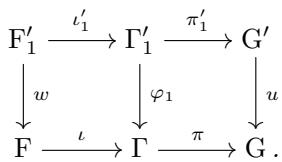
\includegraphics[keepaspectratio]{images/part002_e5b6b945.jpg}}

则存在唯一的群同态 \(\psi : \Gamma_1' \to \Gamma'\)，使得图

\pandocbounded{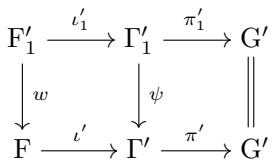
\includegraphics[keepaspectratio]{images/part002_7bcd6e81.jpg}}

交换且 \(\varphi_{1} = \varphi \circ \psi\)。

若群同态 \(\psi : \Gamma_1' \to \Gamma'\) 具有所要的性质，则它满足关系

\[
\psi (\gamma) = (\varphi \circ \psi (\gamma), \pi^ {\prime} \circ \psi (\gamma)) = (\varphi_ {1} (\gamma), \pi_ {1} ^ {\prime} (\gamma))
\]

（对每个 \(\gamma \in \Gamma_1'\)）。反之，从 \(\Gamma_1'\) 到 \(\Gamma \times G'\) 的由 \(\gamma \mapsto (\varphi_1(\gamma), \pi_1'(\gamma))\) 定义的群同态取值在纤维积 \(\Gamma \times_G G'\) 中，因为 \(\pi \circ \varphi_1(\gamma) = u \circ \pi_1'(\gamma)\)（对每个 \(\gamma \in \Gamma_1'\)）。

推论 1. —— 设 \(E_{1}\) 与 \(E_{2}\) 是 G 被 F 的 \(\tau\)-扩张，并设 \(\psi\) 是一个 \(\tau\)-扩张的态射（从 \(E_{1}\) 到 \(E_{2}\) 的）。用 \(\varphi_{1}\)（相应地，\(\varphi_{2}\)）表示 \(u^{*}(\mathcal{E}_{1})\)（相应地，\(u^{*}(\mathcal{E}_{2})\)）的典范同态。则存在唯一的 \(\tau'\)-扩张的态射（从 \(u^{*}(\mathcal{E}_{1})\) 到 \(u^{*}(\mathcal{E}_{2})\) 的），记作 \(u^{*}(\psi)\)，使得 \(\varphi_{2} \circ u^{*}(\psi) = \psi \circ \varphi_{1}\)。

只需对 \(\psi \circ \varphi_{1}\) 应用命题 1。

于是 \(\tau^{\prime}\)-扩张 \(u^{*}(\mathcal{E})\) 的类只依赖于 E 的类。我们也用 \(u^{*}:\operatorname{Ex}_{\tau}(\mathrm{G},\mathrm{F})\to\operatorname{Ex}_{\tau^{\prime}}(\mathrm{G}^{\prime},\mathrm{F})\) 表示把一个 \(\tau\)-扩张 E 的类映到 \(\tau^{\prime}\)-扩张 \(u^{*}(\mathcal{E})\) 的类的映射。

推论 2. —— 设 \(u': G'' \to G'\) 是一个群同态，\(\mathcal{E}\) 是 G 被 F 的一个 \(\tau\)-扩张。设 \(\tau'' = \tau' \circ u'\)，并用 \(\varphi\)（相应地，\(\varphi', \varphi''\)）表示与 \(\tau'\)-扩张 \(u^*(\mathcal{E})\)（相应地，\(\tau''\)-扩张 \(u'^*(u^*(\mathcal{E}))\)、\(\tau''\)-扩张 \((u \circ u')^*(\mathcal{E})\)）相伴的典范同态。则存在唯一的态射 \(\psi\)（从 \(\tau''\)-扩张 \(u'^*(u^*(\mathcal{E}))\) 到 \(\tau''\)-扩张 \((u \circ u')^*(\mathcal{E})\) 的），使得 \(\varphi'' \circ \psi = \varphi \circ \varphi'\)。

例. —— 设 H 是 G 的一个子群，\(j : H \to G\) 是典范单射。则对每个 \(\tau\)-扩张 \(\mathcal{E} = (\Gamma, \iota, \pi)\)，\(\tau \circ j\)-扩张 \(j^{*}(\mathcal{E})\) 同构于 \((\bar{\pi}^{1}(H), \iota', \pi')\)，其中 \(\iota' : F \to \bar{\pi}^{1}(H)\)（相应地，\(\pi' : \bar{\pi}^{1}(H) \to H\)）是群同态 \(f \mapsto \iota(f)\)（相应地，\(\gamma \mapsto \pi(\gamma)\)）。更一般地，若群同态 \(u : G' \to G\) 是单射的，则典范同态 \(\varphi\) 是单射的，其像为 \(\bar{\pi}^{1}(u(G'))\)。

\subsection{\texorpdfstring{\(\tau\)-扩张的直像}{\textbackslash tau-扩张的直像}}

设 G 是一个群，设 F 与 \(F'\) 是交换群，设 \(\tau\)（相应地，\(\tau'\)）是一个群同态（从 G 到 F（相应地，\(F'\)）的自同构群的），并设 \(v: F \to F'\) 是一个群同态，使得

\[
v (\tau (g) \cdot f) = \tau^ {\prime} (g) \cdot v (f)\tag{3}
\]

（对每个 \(g \in G\) 与 \(f \in F\)）。设 \(\mathcal{E} = (\Gamma, \iota, \pi)\) 是 G 被 F 的一个 \(\tau\)-扩张。设 \(\widetilde{\Gamma}\) 是外半直积 \(F' \times_{\tau' \circ \pi} \Gamma\)。用 \(\widetilde{\iota}: F' \to \widetilde{\Gamma}\) 表示同态 \(f \mapsto (f, e)\)，并用 \(\widetilde{p}: \widetilde{\Gamma} \to \Gamma\) 表示第一个投影。设 \(j: F \to \widetilde{\Gamma}\) 是由 \(f \mapsto (v(f), \iota(f)^{-1})\) 定义的映射。由于 \(\iota\) 的像包含在 \(\tau' \circ \pi\) 的核中，映射 j 是一个群同态；由于 \(\iota\) 是单射的，它是单射的。我们有关系

\[
\begin{array}{r l} (f ^ {\prime}, \gamma) j (f) (f ^ {\prime}, \gamma) ^ {- 1} & = (f ^ {\prime}, \gamma) (v (f), \iota (f) ^ {- 1}) (f ^ {\prime}, \gamma) ^ {- 1} \\ & = (\tau^ {\prime} (\pi (\gamma)) \cdot v (f), \iota (\tau (\pi (\gamma)) \cdot f) ^ {- 1}) \\ & = j (\tau (\pi (\gamma)) \cdot f) \end{array}\tag{4}
\]

（对 \(f \in F\)、\(\gamma \in \Gamma\) 与 \(f' \in F'\)）。因此，j 的像是 \(\widetilde{\Gamma}\) 的一个正规子群。用 \(\Gamma'\) 表示 \(\widetilde{\Gamma}\) 关于 j 的像的商。用 \(\iota'\) 表示从 \(\widetilde{\Gamma}\) 到 \(\Gamma'\) 的典范满射与 \(\widetilde{\iota}\) 的复合。同态 \(\pi \circ \widetilde{p}\) 的核是积 \(\mathrm{F}' \times \iota(\mathrm{F})\)，它包含 j 的像。我们把 \(\pi' : \Gamma' \to G\) 定义为由 \(\pi \circ \widetilde{p}\) 通过过渡到商得到的群同态。由于 \(\iota\) 是单射的，\(j(\mathrm{F})\) 与 \(\widetilde{\iota}(\mathrm{F}')\) 的交化归为 \(\widetilde{\Gamma}\) 的单位元素；由此推出 \(\iota'\) 是单射的。从 \(F' \times F\) 到 \(F' \times \iota(\mathrm{F}) = \operatorname{Ker}(\pi \circ \widetilde{p})\) 的由

\[
(f ^ {\prime}, f) \longmapsto (f ^ {\prime} v (f), \iota (f) ^ {- 1})
\]

给出的映射是一个群同构。于是 \(\iota'\) 的像与 \(\pi'\) 的核重合。由于 \(\pi\) 与 \(\widetilde{p}\) 是满射的，\(\pi'\) 也是满射的。这就证明了 \(\mathcal{E}' = (\Gamma', \iota, \pi')\) 是一个 \(\tau'\)-扩张（\(G\) 被 \(F'\) 的）；我们称它为 \(\mathcal{E}\) 被 \(v\) 的直像，并记作 \(v_{*}(\mathcal{E})\)。从 \(\widetilde{\Gamma}\) 到 \(\Gamma'\) 的典范满射与从 \(\Gamma\) 到 \(\widetilde{\Gamma}\) 的由 \(\gamma \mapsto (1, \gamma)\) 给出的群同态的复合是一个群同态 \(\varphi : \Gamma \to \Gamma'\)，我们称之为典范的。

命题 2. —— 用上面的记号，下面的图交换：

\begin{enumerate}
\def\labelenumi{(\arabic{enumi})}
\setcounter{enumi}{4}
\tightlist
\item
\end{enumerate}

\pandocbounded{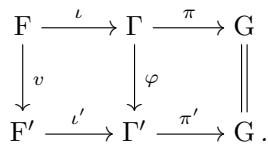
\includegraphics[keepaspectratio]{images/part002_f3abcdb3.jpg}}

设 \(\mathcal{E}_1' = (\Gamma_1', \iota_1', \pi_1')\) 是一个 \(\tau'\)-扩张（G 被 F' 的），并设 \(\varphi_1: \Gamma \to \Gamma_1'\) 是一个使得下图交换的群同态：

\pandocbounded{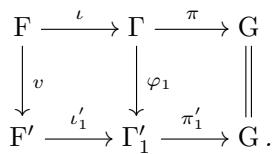
\includegraphics[keepaspectratio]{images/part002_c84edb93.jpg}}

则存在唯一的态射 \(\psi\)（\(\tau'\)-扩张的、从 \(v_{*}(\mathcal{E})\) 到 \(\mathcal{E}_1'\) 的），使得我们有 \(\varphi_1 = \psi \circ \varphi\)。

第一个图的交换性由构造得出。\(\psi\) 的存在性与唯一性由下面的引理 3 得出。

引理 3. —— 设 \(G_{1}^{\prime}\) 是一个群，并设 \(w: G \to G_{1}^{\prime}\) 与 \(\tau_{1}: G_{1}^{\prime} \to \operatorname{Aut}(F^{\prime})\) 是满足 \(\tau^{\prime} = \tau_{1} \circ w\) 的群同态。设 \(\mathcal{E}_{1}^{\prime} = (\Gamma_{1}^{\prime}, \iota_{1}^{\prime}, \pi_{1}^{\prime})\) 是一个 \(\tau_{1}\)-扩张（\(G_{1}^{\prime}\) 被 \(F^{\prime}\) 的），并设 \(\varphi_{1}: \Gamma \to \Gamma_{1}^{\prime}\) 是一个使得下图交换的群同态：

\[
\begin{array}{c} \mathrm{F} \xrightarrow {\iota} \Gamma \xrightarrow {\pi} \mathrm{G} \\ \Biggl \downarrow_ {v} \qquad \qquad \Biggl \downarrow_ {\varphi_ {1}} \qquad \Biggl \downarrow_ {w} \\ \mathrm{F} ^ {\prime} \xrightarrow {\iota_ {1} ^ {\prime}} \Gamma_ {1} ^ {\prime} \xrightarrow {\pi_ {1} ^ {\prime}} \mathrm{G} _ {1} ^ {\prime}. \end{array}
\]

则存在唯一的群同态 \(\psi : \Gamma' \to \Gamma'_1\)，使得图

\[
\begin{array}{c} \mathrm{F} ^ {\prime} \xrightarrow {\iota^ {\prime}} \Gamma^ {\prime} \xrightarrow {\pi^ {\prime}} \mathrm{G} \\ \Big \| \qquad \qquad \qquad \Big \downarrow_ {\psi} \qquad \Big \downarrow_ {w} \\ \mathrm{F} ^ {\prime} \xrightarrow {\iota_ {1} ^ {\prime}} \Gamma_ {1} ^ {\prime} \xrightarrow {\pi_ {1} ^ {\prime}} \mathrm{G} _ {1} ^ {\prime} \end{array}
\]

交换且 \(\varphi_{1} = \psi \circ \varphi\)。

对任何 \((f,\gamma)\in\mathrm{F}^{\prime}\times\Gamma\)，把 \((f,\gamma)\) 在 \(\Gamma^{\prime}\) 中的类记作 \(\overline{(f,\gamma)}\)。若群同态 \(\psi:\Gamma^{\prime}\to\Gamma_{1}^{\prime}\) 具有所要的性质，则它满足关系

\[
\psi \big (\overline {{(f ^ {\prime} , \gamma)}} \big) = \psi (\iota^ {\prime} (f ^ {\prime}) \varphi (\gamma)) = \iota_ {1} ^ {\prime} (f ^ {\prime}) \varphi_ {1} (\gamma)
\]

（对每个 \(f' \in \mathrm{F}'\) 与 \(\gamma \in \Gamma\)）。反之，映射 \(\tilde{\psi}\) 从 \(\mathrm{F}' \times_{\tau' \circ \pi} \Gamma\) 到 \(\Gamma_1'\) 由 \((f, \gamma) \mapsto \iota_1'(f) \varphi_1(\gamma)\) 给出，是一个群同态。实际上，我们有关系

\[
\begin{array}{r} \iota_ {1} ^ {\prime} (f) \varphi_ {1} (\gamma) \iota_ {1} ^ {\prime} (f ^ {\prime}) \varphi_ {1} (\gamma^ {\prime}) = \iota_ {1} ^ {\prime} (f \tau_ {1} (\pi_ {1} ^ {\prime} (\varphi_ {1} (\gamma))) \cdot f ^ {\prime}) \varphi_ {1} (\gamma \gamma^ {\prime}) \\ = \iota_ {1} ^ {\prime} (f \tau^ {\prime} (\pi (\gamma)) \cdot f ^ {\prime}) \varphi_ {1} (\gamma \gamma^ {\prime}) \end{array}
\]

（对 \(f, f' \in \mathrm{F}'\) 与 \(\gamma, \gamma' \in \Gamma\)）。\(\widetilde{\psi}\) 的核包含 \(j\) 的像，因为 \(\iota_1'(v(f)) = \varphi_1(\iota(f))\)（对 \(f \in \mathrm{F}\)），而态射 \(\psi\)（由 \(\widetilde{\psi}\) 通过过渡到商得到的）具有所要的性质。

注. —— 用 \(\Sigma\) 表示 \(\tau'\)-扩张的结构种，并把 \(\alpha\)-映射定义为从 \(\Gamma\) 到群 \(\Gamma'\)（某一个 \(\tau'\)-扩张的底层群）的映射，它们是群同态且使下图交换：

\[
\begin{array}{c} \mathrm{F} \xrightarrow {\iota} \Gamma \xrightarrow {\pi} \mathrm{G} \\ \Big \downarrow v \qquad \qquad \Big \downarrow \varphi \\ \mathrm{F} ^ {\prime} \xrightarrow {\iota^ {\prime}} \Gamma^ {\prime} \xrightarrow {\pi^ {\prime}} \mathrm{G}. \end{array}\tag{6}
\]

命题 2 表示 \(v_{*}(\mathcal{E})\) 是相应的普遍映射问题的一个解（集合论, IV, §3, No.~1, 第 284 页）。

推论 1. —— 设 \(E_{1}\) 与 \(E_{2}\) 是 G 被 F 的 \(\tau\)-扩张，并设 \(\psi\) 是一个 \(\tau\)-扩张的态射（从 \(E_{1}\) 到 \(E_{2}\) 的）。用 \(\varphi_{1}\)（相应地，\(\varphi_{2}\)）表示 \(v_{*}(\mathcal{E}_{1})\)（相应地，\(v_{*}(\mathcal{E}_{2})\)）的典范同态。则存在唯一的 \(\tau'\)-扩张的态射（从 \(v_{*}(\mathcal{E}_{1})\) 到 \(v_{*}(\mathcal{E}_{2})\) 的），记作 \(v_{*}(\psi)\)，使得 \(\varphi_{2} \circ \psi = v_{*}(\psi) \circ \varphi_{1}\)。

只需对 \(\varphi_{2} \circ \psi\) 应用命题 2。

于是 \(\tau^{\prime}\)-扩张 \(v_{*}(\mathcal{E})\) 的类只依赖于 E 的类。我们也用 \(v_{*}:\operatorname{Ex}_{\tau}(\mathrm{G},\mathrm{F})\to\operatorname{Ex}_{\tau^{\prime}}(\mathrm{G},\mathrm{F}^{\prime})\) 表示把一个 \(\tau\)-扩张 E 的类映到 \(\tau^{\prime}\)-扩张 \(v_{*}(\mathcal{E})\) 的类的映射。

推论 2. —— 我们保留命题的记号。设 F'' 是一个交换群，并设 \(\tau'' : G \to \text{Aut}(F'')\) 与 \(v': F' \to F''\) 是满足

\[
\tau^ {\prime \prime} (g) \cdot v ^ {\prime} (f) = v ^ {\prime} (\tau^ {\prime} (g) \cdot f)
\]

（对 \(g \in G\) 与 \(f \in F'\)）的群同态。设 E 是 G 被 F 的一个 \(\tau\)-扩张，并用 \(\varphi\)（相应地，\(\varphi'\)、\(\varphi''\)）表示与 \(v_{*}(\mathcal{E})\)（相应地，\(v_{*}'(v_{*}(\mathcal{E}))\)、\((v' \circ v)_{*}(\mathcal{E})\)）相伴的典范同态。则存在唯一的态射 \(\psi\)（从 \(\tau''\)-扩张 \(v_{*}'(v_{*}(\mathcal{E}))\)（G 被 \(F''\) 的）到 \(\tau''\)-扩张 \((v' \circ v)_{*}(\mathcal{E})\) 的），使得 \(\varphi'' = \psi \circ \varphi' \circ \varphi\)。

例. —— 1) 设 \(j: \{1\} \to \mathrm{F}\) 是典范单射。半平凡扩张 \(\mathcal{I}_{\tau}\) 同构于 \(j_{*}((\mathrm{G}, i, \mathrm{Id}_{\mathrm{G}}))\)，其中 \(i: \{e\} \to \mathrm{G}\) 是典范单射。设 \(c: \mathrm{F} \to \mathrm{F}\) 是常值同态 \(f \mapsto 1\)，并设 \(\mathcal{E}\) 是一个 \(\tau\)-扩张。\(\tau\)-扩张 \(c_{*}(\mathcal{E})\) 也同构于 \(\mathcal{I}_{\tau}\)。

\begin{enumerate}
\def\labelenumi{\arabic{enumi})}
\setcounter{enumi}{1}
\tightlist
\item
  设 E 是 F 的一个在 G 的作用下稳定的子群。用 \(F'\) 表示 F 模 E 的商，用 \(v : F \to F'\) 表示典范同态，并用 \(\tau' : G \to \text{Aut}(F')\) 表示 G 在 \(F'\) 上的作用，它由
\end{enumerate}

\[
\tau^ {\prime} (g) \cdot v (f) = v (\tau (g) \cdot f)
\]

（对 \(g \in G\) 与 \(f \in F\)）刻画。设 \(\mathcal{E} = (\Gamma, \iota, \pi)\) 是 G 被 F 的一个 \(\tau\)-扩张。则 \(\iota(\mathrm{E})\) 是 \(\Gamma\) 的一个正规子群，且 \(\tau'\)-扩张 \(v_{*}(\mathcal{E})\)（G 被 \(F'\) 的）同构于扩张 \((\Gamma/\iota(\mathrm{E}), \bar{\iota}, \overline{\pi})\)，其中 \(\bar{\iota}\) 与 \(\overline{\pi}\) 是由 \(\iota\) 与 \(\pi\) 通过过渡到商得到的群同态。借助这个同构，典范同态 \(\varphi\)（与 \(v_{*}(\mathcal{E})\) 相伴的）对应于从 \(\Gamma\) 到 \(\Gamma/\iota(\mathrm{E})\) 的典范同态。

命题 3. —— 设 G 与 G' 是群，并设 F 与 F' 是交换群。设 \(\tau: \mathrm{G} \to \mathrm{Aut}(\mathrm{F})\)、\(\tau': \mathrm{G} \to \mathrm{Aut}(\mathrm{F}')\)、\(u: \mathrm{G}' \to \mathrm{G}\) 与 \(v: \mathrm{F} \to \mathrm{F}'\) 是满足

\[
\tau^ {\prime} (g) \cdot v (f) = v (\tau (g) \cdot f)
\]

（对 \(g \in G\) 与 \(f \in F\)）的群同态。我们记 \(\tau'' = \tau' \circ u\)。设 E 是 G 被 F 的一个 \(\tau\)-扩张。我们用 \(\varphi_u\)（相应地，\(\varphi_v\)、\(\varphi'_u\)、\(\varphi'_v\)）表示对应于 \(\tau \circ u\)-扩张 \(u^*(\mathcal{E})\)（相应地，\(\tau'\)-扩张 \(v_*(\mathcal{E})\)、\(\tau''\)-扩张 \(u^*(v_*(\mathcal{E}))\) 与 \(v_*(u^*(\mathcal{E})))\)）的典范同态。则存在唯一的态射 \(\psi\)（\(\tau''\)-扩张的，从 \(v_*(u^*(\mathcal{E}))\) 到 \(u^*(v_*(\mathcal{E}))\)），使得 \(\varphi_v \circ \varphi_u = \varphi'_u \circ \psi \circ \varphi'_v\)。

我们把 \(\tau \circ u\)-扩张 \(u^{*}(\mathcal{E})\)（相应地，\(\tau''\)-扩张 \(u^{*}(v_{*}(\mathcal{E}))\)）记作 \((\Gamma_u, \iota_u, \pi_u)\)（相应地，\((\Gamma_u', \iota_u', \pi_u')\)）。把 VIII, 第 287 页的引理 2 应用于 \(\varphi_v \circ \varphi_u\)，我们得到存在一个群同态 \(\psi_{1}:\Gamma_{u}\to\Gamma_{u}^{\prime}\)，使得图

\pandocbounded{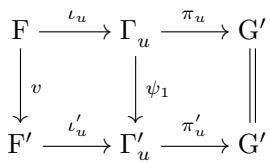
\includegraphics[keepaspectratio]{images/part002_ccea47d6.jpg}}

交换且 \(\varphi_{u}^{\prime}\circ\psi_{1}=\varphi_{v}\circ\varphi_{u}\)。\(\psi\) 的存在性由应用于 \(\psi_{1}\) 的命题 2 得出。反之，若 \(\psi^{\prime}\) 也具有所要的性质，则由引理 2 我们有 \(\psi^{\prime}\circ\varphi_{v}^{\prime}=\psi_{1}\)，故 \(\psi^{\prime}=\psi\)（命题 2）。

\subsection{\texorpdfstring{\(\tau\)-扩张的类上的群律}{\textbackslash tau-扩张的类上的群律}}

设 \(\mathrm{G}\) 是一个群，\(\mathrm{F}\) 是一个交换群，且 \(\tau : \mathrm{G} \to \mathrm{Aut}(\mathrm{F})\) 是一个群同态。用 \(\delta : \mathrm{G} \to \mathrm{G} \times \mathrm{G}\) 表示对角映射 \(g \mapsto (g, g)\)，并用 \(m : \mathrm{F} \times \mathrm{F} \to \mathrm{F}\) 表示乘法同态 \((f_1, f_2) \mapsto f_1 f_2\)。用 \(s : \mathrm{F} \to \mathrm{F}\) 表示由 \(f \mapsto f^{-1}\) 给出的群同态。设 \(\mathcal{E}_1 = (\Gamma_1, \iota_1, \pi_1)\) 与 \(\mathcal{E}_2 = (\Gamma_2, \iota_2, \pi_2)\) 是 \(\tau\)-扩张（\(\mathrm{G}\) 被 \(\mathrm{F}\) 的）。由于我们有关系

\[
m (((\tau \times \tau) \circ \delta) (g) \cdot (f _ {1}, f _ {2})) = \tau (g) \cdot m (f _ {1}, f _ {2})
\]

（对每个 \(g \in G\) 与所有 \(f_{1}, f_{2} \in F\)），扩张 \(m_{*}(\delta^{*}(\mathcal{E}_{1} \times \mathcal{E}_{2}))\) 是一个 \(\tau\)-扩张；我们称它为 \(\tau\)-扩张 \(E_{1}\) 与 \(E_{2}\) 的积，并记作 \(E_{1}E_{2}\)。这个扩张的类只依赖于扩张 \(E_{1}\) 与 \(E_{2}\) 的类（VIII, 第 288 页，推论 1 与 VIII, 第 291 页，推论 1）。于是这在 \(\operatorname{Ex}_{\tau}(\mathbf{G}, \mathbf{F})\) 上给出一个合成律。

注. —— 设 \(\mathcal{E}_{1}=(\Gamma_{1},\iota_{1},\pi_{1})\) 与 \(\mathcal{E}_{2}=(\Gamma_{2},\iota_{2},\pi_{2})\) 是 G 被 F 的 \(\tau\)-扩张。设 \(\mathcal{E}_{1}\mathcal{E}_{2}=(\Gamma,\iota,\pi)\) 是这些扩张的积。仿照 VIII, 第 289 页的例子，该构造给出一个从纤维积 \(\Gamma_{1}\times_{G}\Gamma_{2}\) 到 \(\Gamma\) 的满射群同态，其核是群同态 \(f\mapsto(\iota_{1}(f),\iota_{2}(f)^{-1})\)（从 F 到 \(\Gamma_{1}\times_{G}\Gamma_{2}\)）的像。

命题 4. —— \(\tau\)-扩张的积赋予集合 \(\mathrm{Ex}_{\tau}(\mathrm{G},\mathrm{F})\) 一个交换群的结构。它的单位元素是半平凡扩张 \(\mathcal{I}_{\tau}\) 的类。\(\tau\)-扩张 \(\mathcal{E}\) 的类的逆元是 \(s_{*}(\mathcal{E})\) 的类。

该律的结合性由诸图的交换性

\pandocbounded{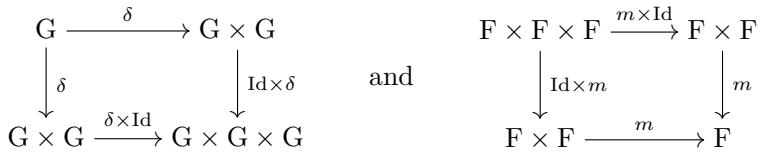
\includegraphics[keepaspectratio]{images/part002_39f17f00.jpg}}

以及 VIII, 第 288 页的推论 2、VIII, 第 291 页的推论 2 与 VIII, 第 292 页的命题 3 得出。

设 \(\Delta : \mathrm{F} \to \mathrm{F} \times \mathrm{F}\) 是对角映射 \(f \mapsto (f, f)\)。设 \(\mathcal{E} = (\Gamma, \iota, \pi)\) 是一个 \(\tau\)-扩张。设 \(\widetilde{\Delta}: \Gamma \to \Gamma \times_{\mathrm{G}} \Gamma\) 是由 \(\gamma \mapsto (\gamma, \gamma)\) 给出的群同态。下图交换：

\pandocbounded{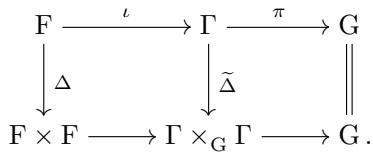
\includegraphics[keepaspectratio]{images/part002_db57599b.jpg}}

由 VIII, 第 290 页的命题 2 推出，\((\tau \times \tau) \circ \delta\)-扩张 \(\delta^{*}(\mathcal{E} \times \mathcal{E})\) 同构于 \(\Delta_{*}(\mathcal{E})\)。

用 \(c: F \to F\) 表示常值同态 \(f \mapsto 1\)。由 VIII, 第 292 页的例 1，\(\mathcal{I}_{\tau}\) 是这个合成律的单位元素这一事实由从 \(\delta^{*}(\mathcal{E} \times \mathcal{E})\) 到 \(\Delta_{*}(\mathcal{E})\) 的同构及交换图

\pandocbounded{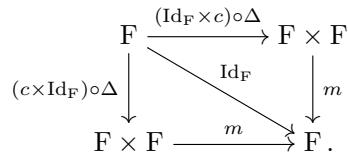
\includegraphics[keepaspectratio]{images/part002_761b87f2.jpg}}

最后一个断言由交换图

\[
\begin{array}{c} \mathrm{F} \xrightarrow {(\mathrm{Id} _ {\mathrm{F}} \times s) \circ \Delta} \mathrm{F} \times \mathrm{F} \\ (s \times \mathrm{Id} _ {\mathrm{F}}) \circ \Delta \Biggl \downarrow \qquad \qquad \qquad \qquad \qquad \qquad \qquad \qquad \qquad \qquad \qquad \qquad \qquad \qquad \qquad \qquad \qquad \qquad \qquad \qquad \qquad \qquad \qquad \qquad \qquad \qquad \qquad \qquad \qquad \qquad \qquad \qquad \qquad \qquad \\ \mathrm{F} \times \mathrm{F} \xrightarrow {m} \mathrm{F}. \end{array}
\]

设 \(\mathcal{E}_1 = (\Gamma_1,\iota_1,\pi_1)\) 与 \(\mathcal{E}_2 = (\Gamma_2,\iota_2,\pi_2)\) 是 \(\tau\)-扩张。群同构 \(\Gamma_1\times \Gamma_2\to \Gamma_2\times \Gamma_1\)（由 \((\gamma_{1},\gamma_{2})\mapsto (\gamma_{2},\gamma_{1})\) 给出）限制为群同构 \(\sigma :\Gamma_1\times_\mathrm{G}\Gamma_2\to \Gamma_2\times_\mathrm{G}\Gamma_1\)。由于关系

\[
\sigma (\iota_ {1} (f), \iota_ {2} (f) ^ {- 1}) = (\iota_ {2} (f ^ {- 1}), \iota_ {1} (f ^ {- 1}) ^ {- 1})
\]

（对 \(f \in F\)），群同态 \(\sigma\) 通过过渡到商诱导出一个 \(\tau\)-扩张的态射（从 \(E_{1}E_{2}\) 到 \(E_{2}E_{1}\) 的）。于是该合成律是交换的。

命题 5. —— a) 设 G 与 G' 是群，并设 F 是一个交换群。设 \(\tau: \mathrm{G} \to \operatorname{Aut}(\mathrm{F})\) 与 \(u: \mathrm{G}' \to \mathrm{G}\) 是群同态。映射 \(u^*: \operatorname{Ex}_{\tau}(\mathrm{G}, \mathrm{F}) \to \operatorname{Ex}_{\tau \circ u}(\mathrm{G}', \mathrm{F})\) 是一个群同态。

\begin{enumerate}
\def\labelenumi{\alph{enumi})}
\setcounter{enumi}{1}
\tightlist
\item
  设 G 是一个群，并设 F 与 \(F'\) 是交换群。设 \(\tau: G \to \text{Aut}(F)\)、\(\tau': G \to \text{Aut}(F')\) 与 \(v: F \to F'\) 是满足
\end{enumerate}

\[
\tau^ {\prime} (g) \cdot v (f) = v (\tau (g) \cdot f)
\]

（对 \(g \in \mathrm{G}\) 与 \(f \in \mathrm{F}\)）的群同态。映射 \(v_{*} : \operatorname{Ex}_{\tau}(\mathrm{G}, \mathrm{F}) \to \operatorname{Ex}_{\tau'}(\mathrm{G}, \mathrm{F}')\) 是一个群同态。

这由诸图的交换性得出

\[
\begin{array}{l} \mathrm{G} ^ {\prime} \xrightarrow {\delta} \mathrm{G} ^ {\prime} \times \mathrm{G} ^ {\prime} \\ \Biggl \downarrow_ {u} \qquad \Biggl \downarrow_ {u \times u} \\ \mathrm{G} \xrightarrow {\delta} \mathrm{G} \times \mathrm{G} \end{array} \qquad \text {and} \qquad \begin{array}{l} \mathrm{F} \times \mathrm{F} \xrightarrow {m} \mathrm{F} \\ \Biggl \downarrow_ {v \times v} \qquad \Biggl \downarrow_ {v} \\ \mathrm{F} ^ {\prime} \times \mathrm{F} ^ {\prime} \xrightarrow {m} \mathrm{F} ^ {\prime}. \end{array}
\]

\subsection{上同调描述}

设 G 是一个群，设 F 是一个交换群，并设 \(\tau: G \to \text{Aut}(F)\) 是一个群同态。对任何 \(g \in G\) 与 \(f \in F\)，我们也用 \(^{g}f\) 表示 \(\tau(g) \cdot f\)。G 的取值于 F 的一个 2-闭上链是指一个映射 \(c: G \times G \to F\)，使得对每个 \((g_{1}, g_{2}, g_{3}) \in G \times G \times G\)，我们有

\[
{ } ^ { g _ { 1 } } c ( g _ { 2 } , g _ { 3 } ) c ( g _ { 1 } , g _ { 2 } g _ { 3 } ) = c ( g _ { 1 } , g _ { 2 } ) c ( g _ { 1 } g _ { 2 } , g _ { 3 } ) .\tag{7}
\]

由于 F 是交换的，2-闭上链所成之集是从 \(G \times G\) 到 F 的映射所成的群的一个子群；我们把它记作 \(Z^{2}(G,F)\)。我们把从 G 到 F 的映射所成的群记作 \(C^{1}(G,F)\)。对每个 \(h \in C^{1}(G,F)\) 与 \((g_{1}, g_{2}) \in G \times G\)，令

\[
(\partial h) (g _ {1}, g _ {2}) = ^ {g _ {1}} h (g _ {2}) h (g _ {1} g _ {2}) ^ {- 1} h (g _ {1}).\tag{8}
\]

一个简单的计算表明映射 \(\partial h: G \times G \to F\) 是一个 2-闭上链。映射 \(\partial: C^{1}(G, F) \to Z^{2}(G, F)\) 是一个群同态。对任何 \(h \in C^{1}(G, F)\)，2-闭上链 \(\partial h\) 称为一个 2-上边缘。群

\(Z^{2}(G,F)/\partial(C^{1}(G,F))\) 记作 \(H^{2}(G,F)\)，称为以 F 为系数群的 G 的第二上同调群。

*上面的记号与 X, §6, n° 8, 第 112 页中关于群上同调的记号一致。*

设 \(\mathcal{E} = (\Gamma, \iota, \pi)\) 是一个 \(\tau\)-扩张。设 \(\sigma\) 是满射映射 \(\pi\) 的一个截面（集合论, II, §3, No.~8, 第 86 页），即一个从 G 到 \(\Gamma\) 的映射，使得 \(\pi(\sigma(g)) = g\)（对 G 中的每个 \(g\)）。对每对 \(g_1, g_2 \in G\)，\(\sigma(g_1)\sigma(g_2)\sigma(g_1g_2)^{-1}\) 属于 \(\mathrm{Ker}(\pi)\)，故存在唯一的映射 \(c_\sigma: G \times G \to F\)，使得

\[
\iota (c _ {\sigma} (g _ {1}, g _ {2})) = \sigma (g _ {1}) \sigma (g _ {2}) \sigma (g _ {1} g _ {2}) ^ {- 1}\tag{9}
\]

（对所有 \(g_{1}, g_{2} \in G\)）。映射 \(c_{\sigma}\) 是常值 1 的当且仅当 \(\sigma\) 是一个群同态。

命题 6. —— 映射 \(c_{\sigma}\) 是群 \(Z^{2}(G,F)\) 的一个元素，且它在上同调群 \(H^{2}(G,F)\) 中的类只依赖于 \(\tau\)-扩张 E 的类。

我们说映射 \(c_{\sigma}\) 是与 \(\sigma\) 相伴的 2-闭上链，而它在 \(\mathrm{H}^2 (\mathrm{G},\mathrm{F})\) 中的上同调类是 \(\tau\)-扩张 \(\mathcal{E}\) 的上同调类。

我们首先验证 \(c_{\sigma}\) 满足闭上链条件。设 \(g_{1}, g_{2}\) 与 \(g_{3}\) 是 G 的元素。利用 VIII, 第 285 页的公式 (1) 与 (9)，我们得到关系

\[
\begin{array}{r l} & {\iota (g _ {1} c _ {\sigma} (g _ {2}, g _ {3}) c _ {\sigma} (g _ {1}, g _ {2} g _ {3}))} \\ & {\quad = \sigma (g _ {1}) \sigma (g _ {2}) \sigma (g _ {3}) \sigma (g _ {2} g _ {3}) ^ {- 1} \sigma (g _ {1}) ^ {- 1} \sigma (g _ {1}) \sigma (g _ {2} g _ {3}) \sigma (g _ {1} g _ {2} g _ {3}) ^ {- 1}} \\ & {\quad = \sigma (g _ {1}) \sigma (g _ {2}) \sigma (g _ {3}) \sigma (g _ {1} g _ {2} g _ {3}) ^ {- 1}} \end{array}
\]

以及

\[
\begin{array}{r l} & {\iota (c _ {\sigma} (g _ {1}, g _ {2}) c _ {\sigma} (g _ {1} g _ {2}, g _ {3}))} \\ & {\qquad = \sigma (g _ {1}) \sigma (g _ {2}) \sigma (g _ {1} g _ {2}) ^ {- 1} \sigma (g _ {1} g _ {2}) \sigma (g _ {3}) \sigma (g _ {1} g _ {2} g _ {3}) ^ {- 1}} \\ & {\qquad = \sigma (g _ {1}) \sigma (g _ {2}) \sigma (g _ {3}) \sigma (g _ {1} g _ {2} g _ {3}) ^ {- 1}.} \end{array}
\]

于是映射 \(c_{\sigma}\) 是 \(\mathbf{Z}^2 (\mathrm{G},\mathrm{F})\) 的一个元素。

我们现在证明 \(c_{\sigma}\) 在 \(\mathrm{H}^{2}(\mathrm{G},\mathrm{F})\) 中的像不依赖于所选取的截面 \(\sigma\)。设 \(\sigma\) 与 \(\sigma'\) 是这样的截面。对 G 的每个元素 g，存在 F 的唯一元素 \(a_{g}\)，使得 \(\sigma'(g) = \iota(a_{g})\sigma(g)\)。设 \(g_{1}\) 与 \(g_{2}\) 是 G 的元素。利用定义 (9)，我们得到等式

\[
\begin{array}{r l} & {\iota (c _ {\sigma^ {\prime}} (g _ {1}, g _ {2})) = \sigma^ {\prime} (g _ {1}) \sigma^ {\prime} (g _ {2}) \sigma^ {\prime} (g _ {1} g _ {2}) ^ {- 1}} \\ & {\qquad = \iota (a _ {g _ {1}}) \sigma (g _ {1}) \iota (a _ {g _ {2}}) \sigma (g _ {2}) \sigma (g _ {1} g _ {2}) ^ {- 1} \iota (a _ {g _ {1} g _ {2}}) ^ {- 1}} \\ & {\qquad = \iota (a _ {g _ {1}}) \iota (^ {g _ {1}} a _ {g _ {2}}) \iota (c _ {\sigma} (g _ {1}, g _ {2})) \iota (a _ {g _ {1} g _ {2}}) ^ {- 1}.} \end{array}\tag{10}
\]

由于群 F 是交换的，我们有关系

\[
c _ {\sigma^ {\prime}} (g _ {1}, g _ {2}) c _ {\sigma} (g _ {1}, g _ {2}) ^ {- 1} = (^ {g _ {1}} a _ {g _ {2}}) a _ {g _ {1} g _ {2}} ^ {- 1} a _ {g _ {1}} = (\partial a) (g _ {1}, g _ {2}),\tag{11}
\]

这由 (8) 得出。这就证明了 \(c_{\sigma'}\) 与 \(c_{\sigma}\) 在 \(\mathrm{H}^2(\mathrm{G},\mathrm{F})\) 中的类重合。

最后，设 \(\mathcal{E} = (\Gamma, \iota, \pi)\) 与 \(\mathcal{E}' = (\Gamma', \iota', \pi')\) 是同构的 \(\tau\)-扩张，设 \(u: \mathcal{E} \to \mathcal{E}'\) 是一个 \(\tau\)-扩张的态射，并设 \(\sigma\) 是映射 \(\pi\) 的一个截面。映射 \(u \circ \sigma\) 是映射 \(\pi'\) 的一个截面，且我们有 \(c_{\sigma} = c_{u \circ \sigma}\)。于是 \(c_{\sigma}\) 在 \(\mathrm{H}^2(\mathrm{G}, \mathrm{F})\) 中的类只依赖于 \(\mathcal{E}\) 在 \(\mathrm{Ex}_{\tau}(\mathrm{G}, \mathrm{F})\) 中的类。

我们用 \(\Theta_{\tau}: \operatorname{Ex}_{\tau}(\mathrm{G},\mathrm{F}) \to \mathrm{H}^{2}(\mathrm{G},\mathrm{F})\)，或更简单地用 \(\Theta\)，表示把一个 \(\tau\)-扩张 \((\Gamma,\iota,\pi)\) 的类映到 2-闭上链 \(c_{\sigma}\) 的类的映射，其中 \(\sigma\) 是满射 \(\pi\) 的一个截面。

定理 1. —— 映射 \(\Theta\) 是从 \(\operatorname{Ex}_{\tau}(\mathrm{G},\mathrm{F})\) 到 \(\mathrm{H}^2 (\mathrm{G},\mathrm{F})\) 的一个群同构。

我们首先证明 \(\Theta\) 是一个群同态。设 \(\mathcal{E} = (\Gamma, \iota, \pi)\) 与 \(\mathcal{E}' = (\Gamma', \iota', \pi')\) 是 \(\tau\)-扩张，并设 \(\sigma\)（相应地，\(\sigma'\)）是映射 \(\pi\)（相应地，\(\pi'\)）的一个截面。我们用 \(\mathcal{E}\mathcal{E}' = (\Gamma'', \iota'', \pi'')\) 表示 \(\tau\)-扩张 E 与 \(E'\) 的积。我们用 \([\gamma, \gamma']\) 表示 \(\Gamma''\) 的元素，即元素 \((\gamma, \gamma')\)（\(\Gamma \times_{G} \Gamma'\) 中的）经 VIII, 第 293 页的注中的满射同态所得到的像。从 G 到 \(\Gamma''\) 的、把元素 g 映到 \([\sigma(g), \sigma'(g)]\) 的映射是一个截面 \(\sigma''\)（映射 \(\pi''\) 的）。设 \(g_1\) 与 \(g_2\) 是 G 的元素。我们有关系

\[
\begin{array}{r l} & {\iota^ {\prime \prime} (c _ {\sigma^ {\prime \prime}} (g _ {1}, g _ {2})) = \sigma^ {\prime \prime} (g _ {1}) \sigma^ {\prime \prime} (g _ {2}) \sigma^ {\prime \prime} (g _ {1} g _ {2}) ^ {- 1}} \\ & {\qquad = [ \iota (c _ {\sigma} (g _ {1}, g _ {2})), \iota^ {\prime} (c _ {\sigma^ {\prime}} (g _ {1}, g _ {2}) ]} \\ & {\qquad = \iota^ {\prime \prime} (c _ {\sigma} (g _ {1}, g _ {2}) c _ {\sigma^ {\prime}} (g _ {1}, g _ {2})).} \end{array}
\]

于是我们有 \(c_{\sigma''}(g_1, g_2) = c_\sigma(g_1, g_2)c_{\sigma'}(g_1, g_2)\)。

我们证明映射 \(\Theta\) 是单射。设 \(\mathcal{E} = (\Gamma, \iota, \pi)\) 是一个 \(\tau\)-扩张，并设 \(\sigma\) 是映射 \(\pi\) 的一个截面，使得 \(c_{\sigma}\) 在 \(\mathrm{H}^{2}(\mathrm{G}, \mathrm{F})\) 中的像是平凡的。存在一个映射 \(a : G \to F\)，使得

\[
c _ {\sigma} (g _ {1}, g _ {2}) = (^ {g _ {1}} a (g _ {2})) a (g _ {1} g _ {2}) ^ {- 1} a (g _ {1})
\]

对所有 \(g_{1}, g_{2} \in G\)。然后我们用下式定义 \(\sigma' : G \to \Gamma\)

\[
\sigma^ {\prime} (g) = \iota (a (g) ^ {- 1}) \sigma (g)
\]

对 \(g \in G\)。利用 (11)，我们得到 \(c_{\sigma'}\) 是取常值 1 的映射；于是 \(\sigma'\) 是一个群同态，这就证明了 \(\tau\)-扩张 E 是半平凡的（I, §6, No.~1, 第 67 页, 命题 4）。

我们证明映射 \(\Theta\) 是满射。设 c 是 \(Z^{2}(G,F)\) 的一个元素。我们给集合 \(\Gamma = F \times G\) 赋以如下的合成律：

\[
(f _ {1}, g _ {1}) (f _ {2}, g _ {2}) = \left(f _ {1} (^ {g _ {1}} f _ {2}) c (g _ {1}, g _ {2}), g _ {1} g _ {2}\right)\tag{12}
\]

对所有 \(f_{1}, f_{2} \in F\) 与 \(g_{1}, g_{2} \in G\)。我们有关系

\[
\begin{array}{r l} (f _ {1}, g _ {1}) ((f _ {2}, g _ {2}) (f _ {3}, g _ {3})) & = (f _ {1}, g _ {1}) \big (f _ {2} (^ {g _ {2}} f _ {3}) c (g _ {2}, g _ {3}), g _ {2} g _ {3} \big) \\ & = \big (f _ {1} (^ {g _ {1}} f _ {2}) (^ {g _ {1} g _ {2}} f _ {3}) (^ {g _ {1}} c (g _ {2}, g _ {3})) c (g _ {1}, g _ {2} g _ {3}), g _ {1} g _ {2} g _ {3} \big) \end{array}
\]

以及

\[
\begin{array}{c} ((f _ {1}, g _ {1}) (f _ {2}, g _ {2}))   (f _ {3}, g _ {3}) = \big (f _ {1} (^ {g _ {1}} f _ {2}) c (g _ {1}, g _ {2}), g _ {1} g _ {2} \big) (f _ {3}, g _ {3}) \\ = \big (f _ {1} (^ {g _ {1}} f _ {2}) (^ {g _ {1} g _ {2}} f _ {3}) c (g _ {1}, g _ {2}) c (g _ {1} g _ {2}, g _ {3}), g _ {1} g _ {2} g _ {3} \big) \end{array}
\]

对所有 \(f_{1}, f_{2}, f_{3} \in F\) 与 \(g_{1}, g_{2}, g_{3} \in G\)。由此推出该律是结合的，因为 c 是一个 2-闭上链。对每个 \((f, g) \in \Gamma\)，我们有

\[
(f, g) (c (e, e) ^ {- 1}, e) = (f (^ {g} c (e, e) ^ {- 1}) c (g, e), g).
\]

另一方面，由 2-闭上链的定义推出 \(c(g, e) = {}^g c(e, e)\)，由此我们推出 \((f, g)(c(e, e)^{-1}, e) = (f, g)\)。我们同理证明

\[
(c (e, e) ^ {- 1}, e) (f, g) = (f c (e, e) ^ {- 1} c (e, g), g) = (f, g).
\]

于是由 (12) 定义的合成律有单位元素 \((c(e,e)^{-1},e)\)，且每个元素 \((f,g)\)（属于 \(\Gamma\)）都是可逆的，其逆为

\[
\left(^ {g ^ {- 1}} (f ^ {- 1} c (e, e) ^ {- 1} c (g, g ^ {- 1}) ^ {- 1}), g ^ {- 1}\right).
\]

这样我们就给 \(\Gamma\) 装备了一个群结构。我们用 \(\iota: F \to G\) 表示把 f 映到 \((c(e, e)^{-1}f, e)\) 的映射，用 \(\pi: \Gamma \to G\) 表示第二个投影，并用 \(\sigma\) 表示映射 \(g \mapsto (1, g)\)。映射 \(\iota\) 与 \(\pi\) 是群同态，于是三元组 \(\mathcal{E} = (\Gamma, \iota, \pi)\) 是一个 \(\tau\)-扩张，\(\sigma\) 是映射 \(\pi\) 的一个截面，并且相伴的闭上链 \(c_{\sigma}\) 等于 c，因为

\[
\begin{array}{c} \sigma (g _ {1}) \sigma (g _ {2}) \sigma (g _ {1} g _ {2}) ^ {- 1} = (1, g _ {1}) (1, g _ {2}) (1, g _ {1} g _ {2}) ^ {- 1} = (c (g _ {1}, g _ {2}), g _ {1} g _ {2}) (1, g _ {1} g _ {2}) ^ {- 1} \\ = (c (g _ {1}, g _ {2}) c (e, g _ {1} g _ {2}) ^ {- 1}, e) = (c (e, e) ^ {- 1} c (g _ {1}, g _ {2}), e) \end{array}
\]

对 \(g_{1}, g_{2} \in G\)。

注. —— 设 G 是一个群，设 F 与 \(F'\) 是交换群， 设 \(\tau\)（相应地，\(\tau'\)）是从 G 到 F（相应地，\(F'\)）的自同构群的一个群同态，并设 \(v : F \to F'\) 是一个群态射，使得

\[
v (\tau (g) \cdot f) = \tau^ {\prime} (g) \cdot v (f)\tag{13}
\]

对 \(g \in G\) 与 \(f \in F\)。设 \(\alpha\) 是 \(\operatorname{Ex}_{\tau}(\mathrm{G}, \mathrm{F})\) 的一个元素。若闭上链 c 代表 \(\Theta(\alpha)\)，则 \(v \circ c\) 代表 \(\Theta(v_{*}(\alpha)) \in \mathrm{H}^{2}(\mathrm{G}, \mathrm{F}')\)。

\subsection{限制与余限制}

设 G 与 \(G'\) 是群，F 是交换群，而 \(\tau\) 是从 G 到 F 的自同构群的一个同态。设 \(u: G' \to G\) 是一个群同态。我们记 \(\tau' = \tau \circ u\)。

若 \(\psi : \mathrm{G} \times \mathrm{G} \to \mathrm{F}\) 是 \(\mathrm{G}\) 的取值于 \(\mathrm{F}\) 的一个 2-闭上链，则映射 \(\psi \circ (u \times u)\)（从 \(\mathrm{G}' \times \mathrm{G}'\) 到 \(\mathrm{F}\)，由 \((g_1, g_2) \mapsto \psi(u(g_1), u(g_2))\) 给出）是 \(\mathrm{G}'\) 的取值于 \(\mathrm{F}\) 的一个 2-闭上链，且映射 \(\psi \mapsto \psi \circ (u \times u)\)（从 \(\mathrm{Z}^2(\mathrm{G}, \mathrm{F})\) 到 \(\mathrm{Z}^2(\mathrm{G}', \mathrm{F})\)）诱导一个群同态 \(u^*: \mathrm{H}^2(\mathrm{G}, \mathrm{F}) \to \mathrm{H}^2(\mathrm{G}', \mathrm{F})\)。对任何 \(\lambda \in \mathrm{H}^2(\mathrm{G}, \mathrm{F})\)，元素 \(u^*(\lambda)\) 称为 \(\lambda\) 被 \(u\) 的逆像。当 \(\mathrm{G}'\) 是 \(\mathrm{G}\) 的子群且 \(u: \mathrm{G}' \to \mathrm{G}\) 是典范单射时，同态 \(u^*\) 称为从 \(\mathrm{G}\) 到 \(\mathrm{G}'\) 的限制同态；我们把它记作 \(\operatorname{Res}_{\mathrm{G}'}^{\mathrm{G}}\)。当 \(\mathrm{G}\) 是 \(\mathrm{G}'\) 的商且 \(u: \mathrm{G}' \to \mathrm{G}\) 是典范满射时，同态 \(u^*\) 称为从 \(\mathrm{G}\) 到 \(\mathrm{G}'\) 的膨胀同态。

命题 7. —— 用上面的记号，下图交换：

\[
\begin{array}{c} \operatorname{Ex} _ {\tau} (\mathrm{G}, \mathrm{F}) \xrightarrow {u ^ {*}} \operatorname{Ex} _ {\tau} (\mathrm{G} ^ {\prime}, \mathrm{F}) \\ \Biggl \downarrow \Theta_ {\tau} \qquad \qquad \qquad \Biggl \downarrow \Theta_ {\tau^ {\prime}} \\ \operatorname{H} ^ {2} (\mathrm{G}, \mathrm{F}) \xrightarrow {u ^ {*}} \operatorname{H} ^ {2} (\mathrm{G} ^ {\prime}, \mathrm{F})  . \end{array}
\]

设 H 是 G 的一个有限指数子群。设 s 是从 G 到 \(H\backslash G\) 的典范满射的一个截面。我们用 \((g,x)\mapsto x\cdot g\) 表示由 G 借乘法在其自身上的右作用所诱导的 G 在 \(H\backslash G\) 上的右作用。注意对每个 \(x\in H\backslash G\) 与 \(g\in G\)，元素 \(s(x)gs(x\cdot g)^{-1}\) 属于 H。于是对任何映射 \(c: \mathrm{H} \times \mathrm{H} \to \mathrm{F}\)，我们都可以用关系式定义一个映射 \(\widetilde{c}_s: \mathrm{G} \times \mathrm{G} \to \mathrm{F}\)

\[
\widetilde {c} _ {s} (g _ {1}, g _ {2}) = \prod_ {x \in \mathrm{H} \backslash \mathrm{G}} ^ {s (x) ^ {- 1}} c \bigl (s (x) g _ {1} s (x \cdot g _ {1}) ^ {- 1}, s (x \cdot g _ {1}) g _ {2} s (x \cdot g _ {1} g _ {2}) ^ {- 1} \bigr)
\]

对 \(g_{1}, g_{2} \in G\)。映射 \(c \mapsto \widetilde{c}_{s}\) 是从 \(F^{H \times H}\) 到 \(F^{G \times G}\) 的一个群同态。

引理 4. —— 若 \(c: \mathrm{H} \times \mathrm{H} \to \mathrm{F}\) 是 H 的取值于 F 的一个 2-闭上链，则 \(\widetilde{c}_s\) 是 G 的取值于 F 的一个 2-闭上链。

设 \(g_1, g_2\) 与 \(g_3\) 是 G 的元素。对每个 \(i \in \{1, 2, 3\}\)，我们用关系式定义一个映射 \(h_i: \mathrm{H} \backslash \mathrm{G} \to \mathrm{H}\)

\[
h _ {i} (x) = s \left(x \cdot g _ {1} \dots g _ {i - 1}\right) g _ {i} s \left(x \cdot g _ {1} \dots g _ {i}\right) ^ {- 1}
\]

对 \(x\in \mathrm{H}\backslash \mathrm{G}\)。注意

\[
\begin{array}{l} {h _ {1} (x) h _ {2} (x) = s (x) g _ {1} g _ {2} s (x \cdot g _ {1} g _ {2}) ^ {- 1}} \\ {h _ {2} (x) h _ {3} (x) = s (x \cdot g _ {1}) g _ {2} g _ {3} s (x \cdot g _ {1} g _ {2} g _ {3}) ^ {- 1}} \end{array}
\]

对 \(x \in \mathrm{H} \backslash \mathrm{G}\)。于是我们有关系

\[
\begin{array}{r l} & ^ {g _ {1}} \widetilde {c} _ {s} (g _ {2}, g _ {3}) \widetilde {c} _ {s} (g _ {1} g _ {2}, g _ {3}) ^ {- 1} \widetilde {c} _ {s} (g _ {1}, g _ {2} g _ {3}) \widetilde {c} _ {s} (g _ {1}, g _ {2}) ^ {- 1} \\ & \quad = \prod_ {x \in \mathrm{H} \backslash \mathrm{G}} ^ {g _ {1} s (x) ^ {- 1}} c \big (s (x) g _ {2} s (x \cdot g _ {2}) ^ {- 1}, s (x \cdot g _ {2}) g _ {3} s (x \cdot g _ {2} g _ {3}) ^ {- 1} \big) \\ & \qquad \times \prod_ {x \in \mathrm{H} \backslash \mathrm{G}} ^ {s (x) ^ {- 1}} \Big (c (h _ {1} (x) h _ {2} (x), h _ {3} (x)) ^ {- 1} \\ & \qquad \qquad \qquad \qquad \times c (h _ {1} (x), h _ {2} (x) h _ {3} (x))   c (h _ {1} (x), h _ {2} (x)) ^ {- 1} \Big) \\ & = \prod_ {x \in \mathrm{H} \backslash \mathrm{G}} ^ {s (x \cdot g _ {1} ^ {- 1}) ^ {- 1} h _ {1} (x \cdot g _ {1} ^ {- 1})} c (h _ {2} (x \cdot g _ {1} ^ {- 1}), h _ {3} (x \cdot g _ {1} ^ {- 1})) \\ & \qquad \times \prod_ {x \in \mathrm{H} \backslash \mathrm{G}} ^ {s (x) ^ {- 1} h _ {1} (x)} c (h _ {2} (x), h _ {3} (x)) ^ {- 1} \\ & = 1, \end{array}
\]

其中第二个等式由 c 是 2-闭上链这一事实得出。

引理 5. —— 若 \(c\) 是一个 2-上边缘，则 \(\widetilde{c}_s\) 也是。

设 \(t: \mathrm{H} \to \mathrm{F}\) 是使得 \(c = \partial t\) 的一个映射。设 \(\widetilde{t}_s: \mathrm{G} \to \mathrm{F}\) 是由下式定义的映射

\[
\widetilde {t} _ {s} (g) = \prod_ {x \in \mathrm{H} \backslash \mathrm{G}} ^ {s (x) ^ {- 1}} t (s (x) g s (x \cdot g) ^ {- 1})
\]

对 \(g \in G\)。只需证明 \(\widetilde{c}_{s} = \partial\widetilde{t}_{s}\)，这由关系

\[
\begin{array}{l} \widetilde {c} _ {s} (g _ {1}, g _ {2}) = \prod_ {x \in \mathrm{H} \backslash \mathrm{G}} ^ {s (x) ^ {- 1} s (x) g _ {1} s (x \cdot g _ {1}) ^ {- 1}} t (s (x \cdot g _ {1}) g _ {2} s (x \cdot g _ {1} g _ {2}) ^ {- 1}) \\ \qquad \times \prod_ {x \in \mathrm{H} \backslash \mathrm{G}} ^ {s (x) ^ {- 1}} \big (t (s (x) g _ {1} g _ {2} s (x \cdot g _ {1} g _ {2}) ^ {- 1}) ^ {- 1} t (s (x) g _ {1} s (x \cdot g _ {1}) ^ {- 1}) \big) \\ = \partial \widetilde {t} _ {s} (g _ {1}, g _ {2}) \end{array}
\]

对 \(g_{1}, g_{2} \in G\) 得出。

引理 6. —— 设 c 是 H 的取值于 F 的一个 2-闭上链。\(\widetilde{c}_{s}\) 在群 \(\mathrm{H}^{2}(\mathrm{G},\mathrm{F})\) 中的像不依赖于截面 s 的选取。

设 \(s'\) 是从 G 到 \(H\backslash G\) 的典范满射的一个截面。设 \(h: \mathrm{H} \backslash \mathrm{G} \to \mathrm{H}\) 是由关系式

\[
s ^ {\prime} (x) = h (x) s (x)
\]

对 \(x \in H \backslash G\) 刻画的映射。于是 2-闭上链 \(\widetilde{c}_{s'}\) 由关系式给出

\[
\begin{array}{l} \widetilde {c} _ {s ^ {\prime}} (g _ {1}, g _ {2}) \\ = \prod_ {x \in \mathrm{H} \backslash \mathrm{G}} ^ {s (x) ^ {- 1} h (x) ^ {- 1}} c \big (h (x) s (x) g _ {1} s ^ {\prime} (x \cdot g _ {1}) ^ {- 1}, s ^ {\prime} (x \cdot g _ {1}) g _ {2} s ^ {\prime} (x \cdot g _ {1} g _ {2}) ^ {- 1} \big) \\ = \prod_ {x \in \mathrm{H} \backslash \mathrm{G}} ^ {s (x) ^ {- 1}} c \big (s (x) g _ {1} s (x \cdot g _ {1}) ^ {- 1} h (x \cdot g _ {1}) ^ {- 1}, h (x \cdot g _ {1}) s (x \cdot g _ {1}) g _ {2} s ^ {\prime} (x \cdot g _ {1} g _ {2}) ^ {- 1} \big) \\ \qquad \times \prod_ {x \in \mathrm{H} \backslash \mathrm{G}} ^ {s (x) ^ {- 1}} \Big (c \big (h (x) ^ {- 1}, s ^ {\prime} (x) g _ {1} g _ {2} s ^ {\prime} (x \cdot g _ {1} g _ {2}) ^ {- 1} \big) ^ {- 1} \\ \qquad \qquad \qquad \qquad \qquad \qquad \qquad \qquad \qquad \qquad \qquad \qquad \qquad \qquad \qquad \qquad \qquad \qquad \qquad \qquad \qquad \qquad \qquad \qquad \qquad \qquad \qquad \qquad \qquad \qquad \qquad \qquad \qquad \qquad \\ = \prod_ {x \in \mathrm{H} \backslash \mathrm{G}} ^ {g _ {1} s (x \cdot g _ {1}) ^ {- 1}} c \big (h (x \cdot g _ {1}) ^ {- 1}, h (x \cdot g _ {1}) s (x \cdot g _ {1}) g _ {2} s ^ {\prime} (x \cdot g _ {1} g _ {2}) ^ {- 1} \big) \\ \qquad \times \prod_ {x \in \mathrm{H} \backslash \mathrm{G}} ^ {s (x) ^ - 1} c \big (s (x) g _ {1} s (x \cdot g _ {1}) ^ {- 1}, s (x \cdot g _ {1}) g _ {2} s ^ {\prime} (x \cdot g _ {1} g _ {2}) ^ {- 1} \big) \\ \qquad \times \prod_ {x \in \mathrm{H} \backslash \mathrm{G}} ^ {s (x) ^ {- 1}} c \big (s (x) g _ {1} s (x \cdot g _ {1}) ^ {- 1}, h (x \cdot g _ {1}) ^ {- 1} \big) ^ {- 1} \\ \qquad \times \prod_ {x \in \mathrm{H} \backslash \mathrm{G}} ^ {s (x) ^ {- 1}} \Big (c \big (h (x) ^ {- 1}, s ^ {\prime} (x) g _ {1} g _ {2} s ^ {\prime} (x \cdot g _ {1} g _ {2}) ^ {- 1} \big) ^ {{- 1}} \\ \qquad \qquad \qquad \qquad \qquad \qquad \qquad \qquad \qquad \qquad \qquad \qquad \times c (h (x) ^ {- 1}, s ^ {\prime} (x) g _ {1} s ^ {\prime} (x \cdot g _ {1}) ^ {- 1})   {\Big)} \end{array}
\]

\[
\begin{array}{l} = \prod_ {x \in \mathrm{H} \backslash \mathrm{G}} ^ {s (x) ^ {- 1}} c \big (s (x) g _ {1} s (x \cdot g _ {1}) ^ {- 1}, s (x \cdot g _ {1}) g _ {2} s ^ {\prime} (x \cdot g _ {1} g _ {2}) ^ {- 1} \big) \\ \qquad \times \prod_ {x \in \mathrm{H} \backslash \mathrm{G}} ^ {s (x) ^ {- 1}} c \big (s (x) g _ {1} s (x \cdot g _ {1}) ^ {- 1}, h (x \cdot g _ {1}) ^ {- 1} \big) ^ {- 1} \\ \qquad \times \prod_ {x \in \mathrm{H} \backslash \mathrm{G}} ^ {g _ {1} s (x) ^ {- 1}} c \big (h (x) ^ {- 1}, h (x) s (x) g _ {2} s ^ {\prime} (x \cdot g _ {2}) ^ {- 1} \big) \\ \qquad \times \prod_ {x \in \mathrm{H} \backslash \mathrm{G}} ^ {s (x) ^ {- 1}} \Big (c \big (h (x) ^ {- 1}, s ^ {\prime} (x) g _ {1} g _ {2} s ^ {\prime} (x \cdot g _ {1} g _ {2}) ^ {- 1} \big) ^ {- 1} \\ \qquad \qquad \qquad \qquad \qquad \qquad \qquad \qquad \qquad \qquad \qquad \qquad \qquad \qquad \qquad \qquad \qquad \qquad \times c \big (h (x) ^ {- 1}, s ^ {\prime} (x) g _ {1} s ^ {\prime} (x \cdot g _ {1}) ^ {- 1} \big) \Big) \end{array}
\]

对所有 \(g_1, g_2 \in \mathbf{G}\)。第一个等式来自把闭上链关系（VIII, 第 295 页, 公式 (7)）应用于元素

\[
h (x) ^ {- 1}, \quad h (x) s (x) g _ {1} s ^ {\prime} (x \cdot g _ {1}) ^ {- 1}, \quad \mathrm{and} \quad s ^ {\prime} (x \cdot g _ {1}) g _ {2} s ^ {\prime} (x \cdot g _ {1} g _ {2}) ^ {- 1};
\]

第二个等式是通过对元素

\[
s (x) g _ {1} s \left(x \cdot g _ {1}\right) ^ {- 1}, \quad h \left(x \cdot g _ {1}\right) ^ {- 1}, \quad \text { and } \quad h \left(x \cdot g _ {1}\right) s \left(x \cdot g _ {1}\right) g _ {2} s ^ {\prime} \left(x \cdot g _ {1} g _ {2}\right) ^ {- 1};
\]

而最后一个等式只是用到了映射 \(x \mapsto x \cdot g_{1}\) 是 \(H\backslash G\) 的一个置换这一事实。

所得表达式的最后两行对应于一个 2-上边缘。我们发现 \(\widetilde{c}_{s'}\) 在 \(\mathrm{H}^2 (\mathrm{G},\mathrm{F})\) 中与那个在 \((g_{1},g_{2})\in \mathrm{G}^{2}\) 处的值由下述表达式给出的闭上链有相同的类

\[
\begin{array}{l} \prod_ {x \in \mathrm{H} \backslash \mathrm{G}} ^ {s (x) ^ {- 1}} c \big (s (x) g _ {1} s (x \cdot g _ {1}) ^ {- 1}, s (x \cdot g _ {1}) g _ {2} s (x \cdot g _ {1} g _ {2}) ^ {- 1} h (x \cdot g _ {1} g _ {2}) ^ {- 1} \big) \\ \qquad \qquad \qquad \times \prod_ {x \in \mathrm{H} \backslash \mathrm{G}} ^ {s (x) ^ {- 1}} c \big (s (x) g _ {1} s (x \cdot g _ {1}) ^ {- 1}, h (x \cdot g _ {1}) ^ {- 1} \big) ^ {- 1} \\ = \prod_ {x \in \mathrm{H} \backslash \mathrm{G}} ^ {g _ {1} s (x \cdot g _ {1}) ^ {- 1}} c \big (s (x \cdot g _ {1}) g _ {2} s (x \cdot g _ {1} g _ {2}) ^ {- 1}, h (x \cdot g _ {1} g _ {2}) ^ {- 1} \big) ^ {- 1} \\ \qquad \qquad \times \prod_ {x \in \mathrm{H} \backslash \mathrm{G}} ^ {s (x) ^ {- 1}} c \big (s (x) g _ {1} s (x \cdot g _ {1}) ^ {- 1}, s (x \cdot g _ {1}) g _ {2} s (x \cdot g _ {1} g _ {2}) ^ {- 1} \big) \\ \qquad \qquad \times \prod_ {x \in \mathrm{H} \backslash \mathrm{G}} ^ {s (x) ^ {- 1}} \Big (c \big (s (x) g _ {1} g _ {2} s (x \cdot g _ {1} g _ {2}) ^ {- 1}, h (x \cdot g _ {1} g _ {2}) ^ {- 1} \big) \\ \qquad \qquad \qquad \times c \big (s (x) g _ {1} s (x \cdot g _ {1}) ^ {- 1}, h (x \cdot g _ {1}) ^ {- 1} \big) ^ {- 1} \Big) \end{array}
\]

\[
\begin{array}{l} = \prod_ {x \in \mathrm{H} \backslash \mathrm{G}} ^ {s (x) ^ {- 1}} c \big (s (x) g _ {1} s (x \cdot g _ {1}) ^ {- 1}, s (x \cdot g _ {1}) g _ {2} s (x \cdot g _ {1} g _ {2}) ^ {- 1} \big) \\ \quad \times \prod_ {x \in \mathrm{H} \backslash \mathrm{G}} ^ {g _ {1} s (x) ^ {- 1}} c \big (s (x) g _ {2} s (x \cdot g _ {2}) ^ {- 1}, h (x \cdot g _ {2}) ^ {- 1} \big) ^ {- 1} \\ \quad \times \prod_ {x \in \mathrm{H} \backslash \mathrm{G}} ^ {s (x) ^ {- 1}} \Big (c \big (s (x) g _ {1} g _ {2} s (x \cdot g _ {1} g _ {2}) ^ {- 1}, h (x \cdot g _ {1} g _ {2}) ^ {- 1} \big) \\ \qquad \qquad \qquad \qquad \qquad \qquad \qquad \qquad \qquad \qquad \qquad \qquad \qquad \times c \big (s (x) g _ {1} s (x \cdot g _ {1}) ^ {- 1}, h (x \cdot g _ {1}) ^ {- 1} \big) ^ {- 1} \Big), \end{array}
\]

其中第一个等式由对元素应用闭上链关系得出

\[
s (x) g _ {1} s (x \cdot g _ {1}) ^ {- 1}, \quad s (x \cdot g _ {1}) g _ {2} s (x \cdot g _ {1} g _ {2}) ^ {- 1}, \quad \text { and } \quad h (x \cdot g _ {1} g _ {2}) ^ {- 1}.
\]

所得表达式的最后两行对应于一个 2-上边缘。我们发现 \(\widetilde{c}_{s'}\) 的类与 \(\widetilde{c}_s\) 的类重合。

我们已经构造了一个从群 \(\mathrm{H}^{2}(\mathrm{H},\mathrm{F})\) 到群 \(\mathrm{H}^{2}(\mathrm{G},\mathrm{F})\) 的同态，我们称它为从 H 到 G 的余限制同态，并记作 \(Cor_{H}^{G}\)。

命题 8. —— 设 H 是 G 的一个有限指数子群。自同态 \(Cor_{H}^{G} \circ Res_{H}^{G}\)（群 \(H^{2}(G, F)\) 的）与用指数 \((G : H)\) 作乘法相重合。

设 \(\alpha\) 是 \(\mathrm{H}^2 (\mathrm{G},\mathrm{F})\) 的一个元素，并设 \(c\) 是 \(\mathrm{Z}^2 (\mathrm{G},\mathrm{F})\) 的一个元素，它代表 \(\alpha\)。元素 \(\mathrm{Cor}_{\mathrm{H}}^{\mathrm{G}}\circ \mathrm{Res}_{\mathrm{H}}^{\mathrm{G}}(\alpha)\) 是那个在 \((g_{1},g_{2})\in \mathrm{G}^{2}\) 处的值由下述表达式给出的闭上链的类

\[
\begin{array}{l} \prod_ {x \in \mathrm{H} \backslash \mathrm{G}} ^ {s (x) ^ {- 1}} c (s (x) g _ {1} s (x \cdot g _ {1}) ^ {- 1}, s (x \cdot g _ {1}) g _ {2} s (x \cdot g _ {1} g _ {2}) ^ {- 1}) \\ = \prod_ {x \in \mathrm{H} \backslash \mathrm{G}} c (g _ {1} s (x \cdot g _ {1}) ^ {- 1}, s (x \cdot g _ {1}) g _ {2} s (x \cdot g _ {1} g _ {2}) ^ {- 1}) \\ \quad \times \prod_ {x \in \mathrm{H} \backslash \mathrm{G}} \big (c (s (x) ^ {- 1}, s (x) g _ {1} g _ {2} s (x \cdot g _ {1} g _ {2}) ^ {- 1}) ^ {- 1} c (s (x) ^ {- 1}, s (x) g _ {1} s (x \cdot g _ {1}) ^ {- 1}) \big) \\ = \prod_ {x \in \mathrm{H} \backslash \mathrm{G}} ^ {g _ {1}} c (s (x \cdot g _ {1}) ^ {- 1}, s (x \cdot g _ {1}) g _ {2} s (x \cdot g _ {1} g _ {2}) ^ {- 1}) \\ \quad \times \prod_ {x \in \mathrm{H} \backslash \mathrm{G}} c (g _ {1}, g _ {2} s (x \cdot g _ {1} g _ {2}) ^ {- 1}) c (g _ {1}, s (x \cdot g _ {1}) ^ {- 1}) ^ {- 1} \\ \quad \times \prod_ {x \in \mathrm{H} \backslash \mathrm{G}} \big (c (s (x) ^ {- 1}, s (x) g _ {1} g _ {2} s (x \cdot g _ {1} g _ {2}) ^ {- 1}) ^ {- 1} c (s (x) ^ {- 1}, s (x) g _ {1} s (x \cdot g _ {1}) ^ {- 1}) \big) \end{array}
\]

\[
\begin{array}{l} = \prod_ {x \in \mathrm{H} \backslash \mathrm{G}} c (g _ {1}, g _ {2} s (x \cdot g _ {1} g _ {2}) ^ {- 1}) c (g _ {1}, s (x \cdot g _ {1}) ^ {- 1}) ^ {- 1} \\ \times \prod_ {x \in \mathrm{H} \backslash \mathrm{G}} ^ {g _ {1}} c (s (x) ^ {- 1}, s (x) g _ {2} s (x g _ {2}) ^ {- 1}) \\ \times \prod_ {x \in \mathrm{H} \backslash \mathrm{G}} \left(c (s (x) ^ {- 1}, s (x) g _ {1} g _ {2} s (x \cdot g _ {1} g _ {2}) ^ {- 1}) ^ {- 1} c (s (x) ^ {- 1}, s (x) g _ {1} s (x \cdot g _ {1}) ^ {- 1})\right). \end{array}
\]

第一个等式来自把闭上链关系（VIII, 第 295 页, 公式 (7)）应用于元素

\[
s (x) ^ {- 1}, \quad s (x) g _ {1} s (x \cdot g _ {1}) ^ {- 1}, \quad \mathrm{and} \quad s (x \cdot g _ {1}) g _ {2} s (x \cdot g _ {1} g _ {2}) ^ {- 1};
\]

第二个等式是通过对元素

\[
g _ {1}, \quad s (x \cdot g _ {1}) ^ {- 1}, \quad \mathrm{and} \quad s (x \cdot g _ {1}) g _ {2} s (x \cdot g _ {1} g _ {2}) ^ {- 1}.
\]

通过去掉一个上边缘，我们得到 \(\mathrm{Cor}_{\mathrm{H}}^{\mathrm{G}} \circ \mathrm{Res}_{\mathrm{H}}^{\mathrm{G}}(\alpha)\) 是那个在 \((g_{1}, g_{2}) \in \mathrm{G}^{2}\) 处的值由下述表达式给出的闭上链的类

\[
\begin{array}{l} \prod_ {x \in \mathrm{H} \backslash \mathrm{G}} c (g _ {1}, g _ {2} s (x \cdot g _ {1} g _ {2}) ^ {- 1}) c (g _ {1}, s (x \cdot g _ {1}) ^ {- 1}) ^ {- 1} \\ = \prod_ {x \in \mathrm{H} \backslash \mathrm{G}} ^ {g _ {1}} c (g _ {2}, s (x \cdot g _ {1} g _ {2}) ^ {- 1}) ^ {- 1} c (g _ {1} g _ {2}, s (x \cdot g _ {1} g _ {2}) ^ {- 1}) c (g _ {1}, g _ {2}) \\ \times \prod_ {x \in \mathrm{H} \backslash \mathrm{G}} c (g _ {1}, s (x \cdot g _ {1}) ^ {- 1}) ^ {- 1} \\ = \prod_ {x \in \mathrm{H} \backslash \mathrm{G}} ^ {g _ {1}} c (g _ {2}, s (x \cdot g _ {2}) ^ {- 1}) ^ {- 1} c (g _ {1} g _ {2}, s (x \cdot g _ {1} g _ {2}) ^ {- 1}) c (g _ {1}, s (x \cdot g _ {1}) ^ {- 1}) ^ {- 1} \\ \times c (g _ {1}, g _ {2}) ^ {\text {(G:H)}}, \end{array}
\]

这就证明了结论。

\subsection{伽罗瓦代数}

设 K 是一个交换域。若 E 是一个 K-代数，则我们用 \(\operatorname{Aut}_{\mathrm{K}}(\mathrm{E})\) 表示它的自同构群。若 E 是体 K 的一个伽罗瓦扩张，则群 \(\operatorname{Aut}_{\mathrm{K}}(\mathrm{E})\) 就是伽罗瓦群 \(\operatorname{Gal}(\mathrm{E}/\mathrm{K})\)（V, §10, No.~2, 第 58 页）。

设 G 是一个群。一个 \((K,G)\)-代数是装备了一个群同态 \(\lambda:G\to\operatorname{Aut}_{K}(E)\) 的 K-代数 E。于是同态 \(\lambda\) 给 E 装备了一个以 G 为算子域的带算子群的结构，以及一个左 K{[}G{]}-模的结构，其外部律由下式给出

\[
\Bigl (\sum_ {g \in \mathrm{G}} \mu_ {g} g \Bigr) x = \sum_ {g \in \mathrm{G}} \mu_ {g} \lambda (g). x\tag{14}
\]

对每个 \(x \in \mathrm{L}\) 与每个元素 \((\mu_g)_{g \in \mathrm{G}}\)（\(\mathrm{K}[\mathrm{G}]\) 的）。一个 \((\mathrm{K}, \mathrm{G})\)-代数的态射是一个代数态射，它同时也是一个带算子群的态射。

对每个族 \((\mathrm{E}_{i})_{i\in\mathrm{I}}\)（\((\mathrm{K},\mathrm{G})\)-代数的），装备其带算子群的积群结构的积 K-代数 \(\prod_{i\in I}E_{i}\) 是一个 \((\mathrm{K},\mathrm{G})\)-代数。

若 \(\mathrm{E}\) 是一个 (K, G)-代数，则集合 \(\mathrm{E}^{\mathrm{G}}\)（由 \(\mathrm{E}\) 的在 \(\mathrm{G}\) 下不变的元素组成）是 \(\mathrm{E}\) 的一个子代数。

设 E 是一个 (K, G)-代数，其中 G 经 \(\lambda: G \to \operatorname{Aut}_{\mathrm{K}}(\mathrm{E})\) 作用。若 \(K'\) 是 K 的一个扩张，则对任何 \(g \in G\)，用 \(\lambda'(g)\) 表示自同构 \(\operatorname{Id}_{\mathrm{K}'} \otimes \lambda(g)\)（\(K'\)-代数 \(\operatorname{L}_{(\mathrm{K}')}\) 的）。于是 \(\lambda': g \mapsto \lambda'(g)\) 给 \(\operatorname{L}_{(\mathrm{K}')}\) 装备了一个 \((\mathrm{K}', \mathrm{G})\)-代数的结构。

给定一个群 H 以及 H-集 X 与 Y，我们用 \(\mathcal{F}_{\mathrm{H}}(\mathrm{X},\mathrm{Y})\) 表示从 X 到 Y 的 H-集态射的集合。它是映射 \(f:X\to Y\)（满足 \(f(hx)=hf(x)\)，对每个 \(h\in H\) 与 \(x\in X\)）的集合。

设 G 是一个有单位元素 e 的群，设 H 是 G 的一个子群，并设 E 是一个 (K,H)-代数。由 E 经从 H 到 G 的余诱导得到的 (K,G)-代数，记作 \(\mathrm{Coind}_{\mathrm{H}}^{\mathrm{G}}(\mathrm{E})\)，是装备了 G 的一个作用的 K-代数 \(\mathcal{F}_{\mathrm{H}}(\mathrm{G},\mathrm{E})\)，该作用由同态 \(\lambda\)（从 G 到 \(\mathrm{Aut}_{\mathrm{K}}(\mathrm{Coind}_{\mathrm{H}}^{\mathrm{G}}(\mathrm{E}))\)，由下式定义）给出

\[
(\lambda (g) \cdot f) (g ^ {\prime}) = f (g ^ {\prime} g)\tag{15}
\]

对 \(f \in \text{Coind}_{\text{H}}^{\text{G}}(\text{E})\) 与 \(g, g' \in G\)。

引理 7. —— a) 设 S 是 G 的一个子集，使得 G 的每个元素都可以唯一地写成 hs（其中 \(h \in H\) 与 \(s \in S\)）。于是把 f 映到 \((f(s))_{s \in S}\) 的映射是从 K-代数 \(\operatorname{Coind}_{\mathrm{H}}^{\mathrm{G}}(\mathrm{E})\) 到由 S 到 E 的映射组成的 K-代数 \(\mathcal{F}(\mathrm{S}, \mathrm{E})\) 的一个同构。

\begin{enumerate}
\def\labelenumi{\alph{enumi})}
\setcounter{enumi}{1}
\tightlist
\item
  代数 \(\operatorname{Coind}_{\mathrm{H}}^{\mathrm{G}}(\mathrm{E})\) 在 K 上有有限次数，当且仅当 E 在 K 上有有限次数且 H 在 G 中的指数有限。此时，我们有公式
\end{enumerate}

\[
[ \mathrm{Coind} _ {\mathrm{H}} ^ {\mathrm{G}} (\mathrm{E}): \mathrm{K} ] = (\mathrm{G}: \mathrm{H}) [ \mathrm{E}: \mathrm{K} ].
\]

\begin{enumerate}
\def\labelenumi{\alph{enumi})}
\setcounter{enumi}{2}
\tightlist
\item
  设 \(E^{H}\) 是群 H 在 E 中的不变量代数，而 \(\operatorname{Coind}_{\mathrm{H}}^{\mathrm{G}}(\mathrm{E})^{\mathrm{G}}\) 是群 G 在 \(\operatorname{Coind}_{\mathrm{H}}^{\mathrm{G}}(\mathrm{E})\) 中的不变量代数。映射 \(f \mapsto f(e)\)
\end{enumerate}

从 \(\mathrm{Coind}_{\mathrm{H}}^{\mathrm{G}}(\mathrm{E})\) 到 E 限制为从 \(\mathrm{Coind}_{\mathrm{H}}^{\mathrm{G}}(\mathrm{E})^{\mathrm{G}}\) 到 \(\mathrm{E}^{\mathrm{H}}\) 的一个代数同构。

断言 a) 由定义得出并蕴含 b)。由 (15)，一个从 G 到 E 的映射是 \(\mathrm{Coind}_{\mathrm{H}}^{\mathrm{G}}(\mathrm{E})\) 的在 G 下不变的元素，当且仅当它是常值等于 E 的一个在 H 下不变的元素的映射。

注 1. —— 设 G 是一个群，H 是 G 的一个子群，而 N 是 H 的一个子群。设 E 是一个 (K,N)-代数。设 \(\alpha\) 是 \(\mathcal{F}_{\mathrm{H}}(\mathrm{G},\mathcal{F}_{\mathrm{N}}(\mathrm{H},\mathrm{E}))\) 的一个元素。我们有关系

\[
\alpha (g) (n h) = n (\alpha (g) (h))\tag{16}
\]

对每个 \(g \in \mathbf{G}\)、\(h \in \mathbf{H}\) 与 \(n \in \mathbf{N}\)，以及关系

\[
\alpha (h g) (h ^ {\prime}) = (h \alpha (g)) (h ^ {\prime}) = \alpha (g) (h ^ {\prime} h)\tag{17}
\]

对所有 \(h, h' \in H\) 与每个 \(g \in G\)。因此，\(\alpha(ng)(e) = \alpha(g)(n) = n(\alpha(g)(e))\)（对每个 \(g \in G\) 与 \(n \in N\)）。于是我们可以考虑映射

\[
\psi : \mathcal {F} _ {\mathrm{H}} (\mathrm{G}, \mathcal {F} _ {\mathrm{N}} (\mathrm{H}, \mathrm{E})) \to \mathcal {F} _ {\mathrm{N}} (\mathrm{G}, \mathrm{E})
\]

由关系式 \(\psi(\alpha)(g)=\alpha(g)(e)\)（其中 \(\alpha\) 取遍 \(\mathcal{F}_{\mathrm{H}}(\mathrm{G},\mathcal{F}_{\mathrm{N}}(\mathrm{H},\mathrm{E}))\)，g 取遍 G）定义。映射 \(\psi\) 是从 \(\operatorname{Coind}_{\mathrm{H}}^{\mathrm{G}}(\operatorname{Coind}_{\mathrm{N}}^{\mathrm{H}}(\operatorname{E}))\) 到 \(\operatorname{Coind}_{\mathrm{N}}^{\mathrm{G}}(\operatorname{E})\) 的一个代数同构，其逆把元素 \(\beta\)（\(\mathcal{F}_{\mathrm{N}}(\mathrm{G},\mathrm{E})\) 的）映到映射 \(\alpha\)，后者由关系式 \(\alpha(g)(h)=\beta(hg)\)（对 \(g\in G\) 与 \(h\in H\)）定义。

我们现在假设给定一个有限群 G 以及一个约化的（V, §6, No.~6, 第 32 页）有限次交换 K-代数 L，它装备了由同态 \(\lambda\)（从 G 到 \(\mathrm{Aut}_{\mathrm{K}}(\mathrm{L})\)）所给出的 G 的一个作用。对 \(x \in \mathrm{L}\) 与 \(g \in \mathrm{G}\)，我们用 \(g \cdot x\) 表示 \(x\) 在 L 的自同构 \(\lambda(g)\) 下的变换。设 \(\mathcal{S}\) 是 L 的极大理想的集合；我们用 \(g \cdot \mathfrak{m}\) 表示元素 \(\mathfrak{m}\)（\(\mathcal{S}\) 的）在 L 的自同构 \(\lambda(g)\) 下的变换。它是 \(\mathcal{S}\) 的一个元素。对每个 \(\mathfrak{m}\)（\(\mathcal{S}\) 中的），体 L/ \(\mathfrak{m}\) 是 K 的一个有限扩张。我们用 \(\pi_{\mathfrak{m}}: \mathrm{L} \to \mathrm{L}/\mathfrak{m}\) 表示投影，并用 \(\mathrm{G}_{\mathfrak{m}}\) 表示 \(\mathfrak{m}\) 在 G 中的稳定子，即这样的 \(g \in \mathrm{G}\)（使得 \(g \cdot \mathfrak{m} = \mathfrak{m}\)）组成的集合。K-代数 L/ \(\mathfrak{m}\) 装备了 \(\mathrm{G}_{\mathfrak{m}}\) 的一个作用，它经由同态 \(\lambda_{\mathfrak{m}}\)（从 \(\mathrm{G}_{\mathfrak{m}}\) 到 \(\mathrm{Aut}_{\mathrm{K}}(\mathrm{L}/\mathfrak{m})\)）给出，该同态把元素 \(h\)（\(\mathrm{G}_{\mathfrak{m}}\) 的）映到 L/ \(\mathfrak{m}\) 的、由 \(\lambda(h)\) 通过过渡到商所导出的自同构。

设 \(\mathcal{O}\) 是 G 在 \(\mathcal{S}\) 中的轨道的集合。给定一条轨道 \(\sigma \in \mathcal{O}\)，令 \(\mathfrak{a}_{\sigma} = \bigcap_{\mathfrak{m} \in \sigma} \mathfrak{m}\) 与 \(\mathrm{L}_{\sigma} = \mathrm{L} / \mathfrak{a}_{\sigma}\)。由于 \(\mathfrak{a}_{\sigma}\) 在 G 下不变，通过过渡到商，G 在 L 上的作用定义了一个同态 \(\lambda_{\sigma}\)（从 G 到 \(\mathrm{Aut}_{\mathrm{K}}(\mathrm{L}_{\sigma})\)）。最后，用 \(\pi_{\sigma}\) 表示从 L 到 \(\mathrm{L}_{\sigma}\) 的典范映射。

引理 8. —— a) 对每个 \(g \in G\)、\(\sigma \in \mathcal{O}\) 与 \(\mathfrak{m} \in \sigma\)，我们有

\[
[ \mathrm{L} _ {\sigma}: \mathrm{K} ] = \operatorname{Card} (\sigma) [ \mathrm{L} / \mathfrak {m}: \mathrm{K} ].
\]

\begin{enumerate}
\def\labelenumi{\alph{enumi})}
\setcounter{enumi}{1}
\item
  映射 \(\pi : x \mapsto (\pi_{\sigma}(x))_{\sigma \in \mathcal{O}}\) 是从 L 到 \(\prod_{\sigma \in \mathcal{O}} \mathrm{L}_{\sigma}\) 的一个 (K,G)-代数同构。
\item
  用 \(L^{G}\)（相应地，\(L_{\sigma}^{G}\)）表示 L（相应地，\(L_{\sigma}\)）的在 G 的作用下不变的元素组成的子代数。于是 \(\pi\) 诱导一个从 \(L^{G}\) 到 \(\prod_{\sigma\in\mathcal{O}}L_{\sigma}^{G}\) 的同构。
\end{enumerate}

由于代数 L 是约化的且有限次，L 的极大理想的交化归为 0（VIII, 第 173 页, 推论 2）。此外，若 m 与 \(m'\) 是 L 的两个不同的极大理想，则我们有 \(m + m' = L\)。由 I, §8, No.~11, 第 110 页的命题 10，从 L 到 \(\prod_{m \in S} L/m\) 的典范映射是一个同构，且从 \(L/a_{\sigma}\) 到 \(\prod_{m \in \sigma} L/m\) 的典范映射（对每个 \(\sigma \in O\)）也是同构。断言 a) 由此得出。由于 O 是 S 的一个分拆，断言 b) 成立；断言 c) 是 b) 的直接推论。

我们现在固定一条轨道 \(\sigma \in \mathcal{O}\) 与一个元素 \(\mathfrak{m}\)（\(\sigma\) 的）。令 \(F_{\mathfrak{m}} = \text{Coind}_{G_{\mathfrak{m}}}^{G}(L/\mathfrak{m})\)，并用 \(\lambda_{F_{\mathfrak{m}}}\) 表示 \(G\) 在 \(F_{\mathfrak{m}}\) 上的作用。对任何 \(x \in L\)，用 \(\overline{x}\) 表示从 \(G\) 到 \(L/\mathfrak{m}\) 的、把 \(g\) 映到 \(\pi_{\mathfrak{m}}(gx)\) 的映射。由 VIII, 第 305 页的公式 (15) 以及 \(G_{\mathfrak{m}}\) 在 \(L/\mathfrak{m}\) 上的作用的定义，立即可得 \(\overline{x}\) 属于 \(F_{\mathfrak{m}}\)，且映射 \(u: x \mapsto \overline{x}\)（从 \(L\) 到 \(F_{\mathfrak{m}}\)）满足 \(\lambda_{F_{\mathfrak{m}}}(g) \circ u = u \circ \lambda(g)\)（对 \(g \in G\)）。换言之，\(u\) 是一个 \((K, G)\)-代数的态射。

引理 9. —— 态射 \(u\) 是满射，其核为 \(\mathfrak{a}_{\sigma}\)。由 \(u\) 通过过渡到商得到的映射是从 \(L_{\sigma}\) 到 \(F_{\mathfrak{m}}\) 的一个 (K, G)-代数同构。

由于 \(\pi_{\mathfrak{m}}\) 的核等于 \(\mathfrak{m}\)，\(u\) 的核等于 \(\bigcap_{g\in G}g^{-1}.\mathfrak{m} = \mathfrak{a}_{\sigma}\)。为证明 \(u\) 是满射，只需证明向量空间 \(\mathrm{L}_{\sigma} = \mathrm{L} / \mathfrak{a}_{\sigma}\) 与 \(\mathrm{F}_{\mathfrak{m}}\) 在 \(\mathrm{K}\) 上有相同的维数。而所有理想 \(g\cdot \mathfrak{m}\) 在 \(\mathrm{L}\) 中有相同的余维数，且由引理 8, a)，

\[
[ \mathrm{L} _ {\sigma}: \mathrm{K} ] = \operatorname{Card} (\sigma). [ \mathrm{L} / \mathfrak {m}: \mathrm{K} ].
\]

此外，由引理 7, b)，我们有

\[
[ \mathrm{F} _ {\mathfrak {m}}: \mathrm{K} ] = (\mathrm{G}: \mathrm{G} _ {\mathfrak {m}}) [ \mathrm{L} / \mathfrak {m}: \mathrm{K} ].
\]

由于我们有 \(\operatorname{Card}(\sigma)=(\mathrm{G}:\mathrm{G}_{\mathfrak{m}})\)，我们就证明了等式 \([L_{\sigma}:K]=[F_{m}:K]\)。

我们此外还假设同态 \(\lambda\)（从 G 到 \(\mathrm{Aut}_{\mathrm{K}}(\mathrm{L})\)）是单射。我们借助映射 \(\xi \mapsto \xi \cdot 1\) 把 K 与它在 L 中的像等同起来。设 \(\Omega\) 是 K 的一个代数闭扩张。集合 \(\mathcal{F}(\mathrm{G},\Omega)\)（从 G 到 \(\Omega\) 的映射组成的）与余诱导 \((\Omega ,\mathrm{G})\)-代数 \(\mathrm{Coind}_{\{e\}}^{\mathrm{G}}(\Omega)\) 重合。它是一个秩 1 的自由 \(\Omega [\mathrm{G}]\)-模。设 \(\mathcal{H}\) 是从 L 到 \(\Omega\) 的 K-代数同态的集合。我们定义 G 在 \(\mathcal{H}\) 上的一个右作用，用 \((g,\chi)\mapsto \chi \circ \lambda (g)\)。于是 \(\Omega\)-代数 \(\mathcal{F}(\mathcal{H},\Omega)\) 装备了一个 \((\Omega ,\mathrm{G})\)-代数结构（由 G 在 \(\mathcal{H}\) 上的右作用导出）。

引理 10. —— 设 L 是一个在 K 上平展的 (K, G)-代数。映射 \(\psi\)（从 \(\mathrm{L}_{(\Omega)}\) 到 \(\mathcal{F}(\mathcal{H},\Omega)\)）由关系式

\[
\psi (\xi \otimes x) = (\xi \chi (x)) _ {\chi \in \mathscr {H}}
\]

所刻画，是一个 (K, G)-代数同构。

由于 L 是平展的，映射 \(\psi\) 是一个 \(\Omega\)-代数同构（V, §6, No.~3, 第 30 页, 命题 2 与 V, §6, No.~3, 第 29 页, 命题 1, c)）。我们有关系

\[
\psi ((\operatorname{Id} \otimes \lambda (g)) (\xi \otimes x)) = (\xi (\chi \circ \lambda (g)) (x)) _ {\chi \in \mathscr {H}}
\]

对 \(\xi \in \Omega\)、\(x \in \mathrm{L}\) 与 \(g \in \mathrm{G}\)。于是 \(\psi\) 是一个 \((\Omega, \mathrm{G})\)-代数的态射。

定理 2. —— 设 G 是一个有限群，并设 L 是一个有限次交换 K-代数，它装备了由单同态 \(\lambda\)（从 G 到 \(\operatorname{Aut}_{\mathrm{K}}(\mathrm{L})\)）所给出的 G 的一个作用。下列性质等价：

\begin{enumerate}
\def\labelenumi{(\roman{enumi})}
\item
  存在 G 的一个子群 H、K 的一个有限次伽罗瓦扩张 E、从 H 到 \(\operatorname{Gal}(\operatorname{E}/\operatorname{K})\) 的一个同构，以及一个 \((\operatorname{K},\operatorname{G})\)-代数同构（从 L 到 \(\operatorname{Coind}_{\operatorname{H}}^{\operatorname{G}}(\operatorname{E})\)）。
\item
  代数 L 是平展的，且 H 是一个主齐性 G-集（I, §5, No.~6, 第 60 页, 定义 7）。
\item
  存在一个 \((\Omega,\mathrm{G})\)-代数同构 \(\psi:\mathrm{L}_{(\Omega)}\to\mathcal{F}(\mathrm{G},\Omega)\)；换言之，对每个 \(g\in G\)，自同构 \(\psi\circ\lambda(g)_{(\Omega)}\circ\psi^{-1}\)（\(\Omega^{G}\) 的）等于自同构
\end{enumerate}

\[
(x _ {h}) _ {h \in \mathrm{G}} \longmapsto (x _ {h g}) _ {h \in \mathrm{G}}.
\]

\begin{enumerate}
\def\labelenumi{(\roman{enumi})}
\setcounter{enumi}{3}
\item
  代数 \(\mathrm{L}\) 是约化的，且 \(\mathrm{L}\) 是一个秩 1 的自由 \(\mathrm{K}[\mathrm{G}]\)-模。
\item
  代数 L 是约化的，我们有 \(\operatorname{Card}(G) = [L : K]\)，且 K 是 L 的在 G 的作用下不变的元素组成的子环。
\item
  代数 L 是约化的，群 G 传递地作用在 L 的极大理想的集合上，且对 L 的每个极大理想 m，m 在 G 中的稳定子 \(G_{m}\) 忠实地作用在 L/m 上并以 K 为不变量子域。
\end{enumerate}

(i)⇒(ii)：设 E 是 K 的一个有限次伽罗瓦扩张，而 \(\tau\) 是从 H 到 \(\operatorname{Aut}_{\mathrm{K}}(\mathrm{E})\) 的一个同构。设 S 是 G 模 H 的右陪集的一个代表系。K-代数 \(F = \operatorname{Coind}_{\mathrm{H}}^{\mathrm{G}}(\mathrm{E})\) 同构于 \(\mathcal{F}(\mathrm{S}, \mathrm{E})\)（引理 7, a)）；于是它是平展的。我们用 \(\lambda_{F}\) 表示 G 在 F 上的作用。此外，设 \(\psi\) 是从 E 到 \(\Omega\) 的一个 K-代数同态，并设 \(\chi_{0}\) 是同态 \(f \mapsto \psi(f(e))\)（从 F 到 \(\Omega\)）。设 \(g \in G\) 使得 \(\chi_{0} \circ \lambda_{\mathrm{F}}(g) = \chi_{0}\)；由于 \(\psi\) 是单射，我们于是有 \(f(g) = f(e)\)（对每个 \(f \in F\)）。鉴于引理 7, a)，我们有 \(g \in H\)，且由公式

\[
f (h) = \tau (h) \cdot f (e),\tag{18}
\]

（它对每个 \(h \in H\) 成立），这只可能在 g = e 时发生。另一方面，由引理 7, b) 与 V, §10, No.~6, 第 66 页的定理 3，我们有

\[
[ \mathrm{F}: \mathrm{K} ] = (\mathrm{G}: \mathrm{H}) [ \mathrm{E}: \mathrm{K} ] = (\mathrm{G}: \mathrm{H}) \operatorname{Card} (\mathrm{H}) = \operatorname{Card} (\mathrm{G}).
\]

集合 \(\mathcal{H}\)（从 F 到 \(\Omega\) 的 K-同态组成的）的基数为 {[}F : K{]}，因为 F 是平展的（V, §6, No.~5, 第 32 页, 命题 4），所以 \(\mathrm{Card}(\mathcal{H}) = \mathrm{Card}(\mathrm{G})\)。由于由上所述 \(\chi_0\) 在 G 中的稳定子等于 \(\{e\}\)，\(\mathcal{H}\) 是一个主齐性 G-集。

(ii)⇒(iii)：假设 L 是平展的且 H 是一个主齐性 G-集。由引理 10，\((\Omega,\mathrm{G})\)-代数 \(\mathrm{L}_{(\Omega)}\) 与 \(\mathcal{F}(\mathcal{H},\Omega)\) 同构。由于 H 是一个主齐性 G-集，\((\Omega,\mathrm{G})\)-代数 \(\mathcal{F}(\mathcal{H},\Omega)\) 与 \(\mathcal{F}(\mathrm{G},\Omega)\) 同构。

(iii)⇒(iv)：假设性质 (iii) 成立。于是 \(L_{(\Omega)}\) 是代数 \(\Omega[G]\) 上的一个秩 1 自由模；后者可以典范地与 \(K[G]_{(\Omega)}\) 等同。然后我们应用 VIII, 第 37 页的定理 3。

蕴含关系 \((\mathrm{iv})\Rightarrow (\mathrm{v})\) 是直接的。

我们证明蕴含关系 \((v)\Rightarrow(vi)\)。代数 L 是约化的。由引理 8, c)，群 G 传递地作用在 L 的极大理想的集合 S 上。设 m 是 S 的一个元素。由引理 9，由于 \(\bigcap_{n\in S}n=\{0\}\)，代数 L 同构于代数 \(\operatorname{Coind}_{G_{m}}^{G}(L/m)\)。\(G_{m}\) 在 L/m 中的不变量代数于是由引理 7, c) 与 K 重合。因此同态 \(\lambda_{m}\)（从 \(G_{m}\) 到 \(\operatorname{Gal}((L/m)/K)\)）是满射。此外，由引理 7，我们有

\[
\operatorname{Card} (\mathrm{G}) = [ \mathrm{L}: \mathrm{K} ] = (\mathrm{G}: \mathrm{G} _ {\mathfrak {m}}) [ \mathrm{L} / \mathfrak {m}: \mathrm{K} ].
\]

于是 \(\operatorname{Card}(\mathrm{G}_{\mathfrak{m}}) = [\mathrm{L} / \mathfrak{m}:\mathrm{K}]\)，且同态 \(\lambda_{\mathfrak{m}}\) 是单射。

剩下要证明蕴含关系 \((\mathrm{vi})\Rightarrow(\mathrm{i})\)。设 m 是 L 的一个极大理想。由引理 9，代数 L 同构于代数 \(\operatorname{Coind}_{G_{m}}^{G}(L/m)\)（作为 \((K,G)\)-代数）。由于 \(G_{m}\) 忠实地作用在 L/m 上并以 K 为不变量子域，群同态 \(\lambda_{m}\) 定义了一个从 \(G_{m}\) 到 \(\operatorname{Gal}((L/m)/K)\) 的同构。

注记. —— 2) 在定理 2 中，我们可以把 \(\Omega\) 是代数闭的这一假设换成 \(\Omega\) 是可分闭的这一假设。事实上，若 \(L\) 是平展的，则从 \(L\) 到 \(\Omega\) 的每个 K-代数同态的像都是 \(K\) 的一个可分扩张。

\begin{enumerate}
\def\labelenumi{\arabic{enumi})}
\setcounter{enumi}{2}
\tightlist
\item
  正规基定理（V, §10, No.~9, 第 73 页, 定理 6）是定理 2 中蕴含关系 \((\mathrm{i})\Rightarrow (\mathrm{iv})\) 的一个特例。
\end{enumerate}

定义 1. —— 设 G 是一个有限群，并设 L 是 K 上的一个非零有限次交换代数，它装备了 (K,G)-代数的结构，其中 G 的作用由从 G 到群 \(\operatorname{Aut}_{\mathrm{K}}(\mathrm{L})\) 的一个单同态给出。我们说 L 是一个以 G 为群的伽罗瓦代数，如果它具有定理 2 的那些等价性质 (i) 至 (vi)。

注记. —— 4) 假设 L 是 K 的一个装备了 G 的作用 \(\lambda\) 的扩张。于是 L 是 K 上的一个伽罗瓦代数，当且仅当 L 是 K 的一个伽罗瓦扩张且 \(\lambda\) 是从 G 到 L 在 K 上的伽罗瓦群的一个同构。

\begin{enumerate}
\def\labelenumi{\arabic{enumi})}
\setcounter{enumi}{4}
\tightlist
\item
  假设群 G 是交换的。若 G 忠实且传递地作用在一个集合 X 上，则 X 的任何点的稳定子都化归为单位元（因为 X 的各点的稳定子全都相等，且它们的交化归为 G 的单位元素）。因此，定理 2 的性质 (i) 至 (vi) 也等价于下述性质：
\end{enumerate}

\begin{enumerate}
\def\labelenumi{(\roman{enumi})}
\setcounter{enumi}{6}
\tightlist
\item
  代数 \(\mathrm{L}\) 是平展的，且 \(\mathrm{G}\) 忠实且传递地作用在 \(\mathcal{H}\) 上。
\end{enumerate}

\begin{enumerate}
\def\labelenumi{\arabic{enumi})}
\setcounter{enumi}{5}
\tightlist
\item
  由 V, §10, No.~1, 第 75 页, 引理 5；V, §10, No.~1, 第 76 页, 命题 12；以及 VIII, 第 137 页, 命题 3，伽罗瓦代数是交换的且半单的。
\end{enumerate}

例. —— 1) 设 n 是一个严格正的整数，与 K 的特征指数互素。假设 K 中的 n 次单位根的群 \(\mu_{n}\) 的阶为 n.~于是对 n 的每个因子 d，d 次单位根的群 \(\mu_{d}\) 的阶为 d.~设 a 是 K 的一个非零元素，设 L 是代数 \(\mathrm{K}[\mathrm{X}]/(X^{n}-a)\)，并设 x 是 X 在 L 中的类。序列 \((1,x,\ldots,x^{n-1})\) 是体 K 上的向量空间 L 的一个基，且我们有 \(x^{n}=a\)。此外，多项式

\(X^{n}-a\) 与它的导数 \(nX^{n-1}\) 互素，于是代数 L 是平展的（V, §7, No.~2, 第 37 页, 命题 3）。对每个 \(\zeta\)（\(\mu_{n}\) 中的），自同构 \(P(X)\mapsto P(\zeta X)\)（环 K{[}X{]} 的）通过过渡到商定义了 L 的一个自同态 \(\lambda(\zeta)\)，因为我们有 \((\zeta X)^{n}-a=X^{n}-a\)；它是一个自同构。我们有

\[
\lambda (\zeta) x ^ {i} = \zeta^ {i} x ^ {i}\tag{19}
\]

对 \(0 \leqslant i < n\)。映射 \(\lambda : \zeta \mapsto \lambda(\zeta)\) 是从 \(\mu_{n}\) 到 \(\operatorname{Aut}_{\mathrm{K}}(\mathrm{L})\) 的一个单同态，且群 \(\lambda(\mu_{n})\) 在 L 中的不变量环等于 K·1。由于 \(\mu_{n}\) 的基数等于 \(n = [L : K]\)，装备了 \(\lambda\) 的作用的代数 L 是一个伽罗瓦代数（VIII, 第 308 页, 定理 2, (v)）。

设 \(r\) 是使得 \(a^r\) 属于 \(\mathrm{K}^{*n}\) 的最小严格正整数；它整除 \(n\)，且存在一个元素 \(b\)（\(\mathrm{K}^*\) 的）使得 \(a = b^{n / r}\)。于是（V, §11, No.~8, 第 91 页, 注）多项式 \(\mathrm{X}^r - b\) 不可约，且我们有 \(\mathrm{X}^n - a = \prod_{\zeta \in \mu_{n / r}} (\mathrm{X}^r - \zeta b)\)。设 \(\mathrm{E}\) 是体 \(\mathrm{K}[\mathrm{Y}] / (\mathrm{Y}^r - b)\)，并设 \(y\) 是 \(Y\) 在 \(\mathrm{E}\) 中的类。存在一个同构 \(\theta\)（从 \(\mu_{n / r}\) 到 \(\operatorname{Gal}(\mathrm{E} / \mathrm{K})\)），它由关系式 \(\theta(\xi)(y) = \xi y\) 刻画（V, §11, No.~8, 第 91 页, 例 3）。然后我们验证伽罗瓦代数 \(L\) 同构于 \((K, \mu_n)\)-代数 \(\operatorname{Coind}_{\mu_{n / r}}^{\mu_n}(E)\)。

\begin{enumerate}
\def\labelenumi{\arabic{enumi})}
\setcounter{enumi}{1}
\tightlist
\item
  现在假设体 K 的特征为 \(p \neq 0\)。设 c 是 K 的一个元素。多项式 \(f = X^{p} - X - c\) 与它的导数 \(f' = -1\) 互素，于是代数 \(L = K[X]/(f)\) 是平展的（V, §7, No.~2, 第 37 页, 命题 3）。我们用 x 表示 X 在 L 中的像；我们有关系 \(x^{p} = x + c\)。序列 \((1, x, \ldots, x^{p-1})\) 是把 L 看作 K 上的向量空间时的一个基。
\end{enumerate}

设 P 是 K 的素子域的加法群；它是一个阶为 p 的循环群，由 K 的单位元素 1 生成。对 P 中的每个 j，我们有 \(j^{p} = j\)（V, §1, No.~3, 第 4 页, 公式 (4)），因此 \(f(\mathrm{X} + j) = f(\mathrm{X})\)。故存在代数 L 的一个自同构 \(\gamma(j)\)，它由关系式 \(\gamma(j)(x) = x + j\) 刻画；此外，所得的映射 \(\gamma\) 是从 P 到 \(\operatorname{Aut}_{\mathrm{K}}(\mathrm{L})\) 的一个单同态。

设 \(\Omega\) 是 \(K\) 的一个代数闭扩张，并设 \(\xi\) 是多项式 \(f\) 在 \(\Omega\) 中的一个根。我们有 \(\xi^p = \xi + c\)，于是

\[
\mathrm{X} ^ {p} - \mathrm{X} - c = (\mathrm{X} ^ {p} - \xi^ {p}) - (\mathrm{X} - \xi) = (\mathrm{X} - \xi) ^ {p} - (\mathrm{X} - \xi) = \prod_ {j \in \mathrm{P}} (\mathrm{X} - \xi - j)
\]

由 V, §12, No.~1, 第 94 页, 公式 (1)。对 P 中的每个 \(j\)，存在唯一的代数同态 \(\chi_j: \mathrm{L} \to \Omega\)，它把 \(x\) 映到 \(\xi + j\)；此外，从 L 到 \(\Omega\) 的每个同态都是诸 \(\chi_j\) 之一，且我们有关系 \(\chi_{j}=\chi_{0}\circ\gamma(j)\)。装备了 \(\gamma\) 的代数 L 具有 VIII, 第 308 页的定理 2 的性质 (ii)，因此是 K 上的一个伽罗瓦代数。

为描述 L 的结构，我们必须区分两种情形：

\begin{enumerate}
\def\labelenumi{\alph{enumi})}
\item
  我们有 \(\xi\notin K\)。于是多项式 \(f(X)\) 在 \(K[X]\) 中不可约（V, §11, No.~9, 第 93 页, 例 3）。在这种情形，L 是 K 的一个次数为 p 的循环扩张，且 \(\gamma\) 是从 P 到 \(\operatorname{Gal}(L/K)\) 的一个同构。
\item
  我们有 \(\xi \in \mathrm{K}\)。于是映射 \(\psi : y \mapsto (\chi_j(y))_{j \in \mathrm{P}}\) 是从代数 \(\mathrm{L}\) 到积代数 \(\mathrm{K}^{\mathrm{P}}\) 的一个同构；此外，\(\psi \circ \gamma(k) \circ \psi^{-1}\) 是自同构 \((x_j)_{j \in \mathrm{P}} \mapsto (x_{j+k})_{j \in \mathrm{P}}\)（\(\mathrm{K}^{\mathrm{P}}\) 的，对每个 \(k \in \mathrm{P}\)）。
\end{enumerate}

\subsection{伽罗瓦代数上的作用}

命题 9. —— 设 G 是一个有限群，H 是 G 的一个子群，而 E 是体 K 上的一个以 H 为群的伽罗瓦代数。于是由 E 经从 H 到 G 的余诱导得到的 (K,G)-代数 \(\mathrm{Coind}_{\mathrm{H}}^{\mathrm{G}}(\mathrm{E})\) 是体 K 上的一个以 G 为群的伽罗瓦代数。

由于 E 是 K 上的一个伽罗瓦代数，由 VIII, 第 308 页的定理 2 的性质 (v)，它是约化的，我们有 \(\operatorname{Card}(\mathrm{H}) = [\mathrm{E} : \mathrm{K}]\)，且 K 是 H 在 E 中的不变量环。而由 VIII, 第 305 页的引理 7，代数 \(\mathrm{F} = \operatorname{Coind}_{\mathrm{H}}^{\mathrm{G}}(\mathrm{E})\) 是约化的，且我们有

\[
[ \mathrm{F}: \mathrm{K} ] = (\mathrm{G}: \mathrm{H}) [ \mathrm{E}: \mathrm{K} ] = (\mathrm{G}: \mathrm{H}) \operatorname{Card} (\mathrm{H}) = \operatorname{Card} (\mathrm{G}),
\]

且 \(\mathrm{K}\) 是 \(\mathrm{G}\) 在 \(\mathrm{F}\) 中的不变量环。于是由定理 2, (v) 给出的判别法，\(\mathrm{F}\) 是一个伽罗瓦代数。

命题 10. —— 设 G 是一个有限群。设 L 是体 K 上的一个以 G 为群的伽罗瓦代数，并设 K' 是 K 的一个扩张。于是 (K', G)-代数 \(\mathrm{L}_{(\mathrm{K}')}\) 是 \(K'\) 上的一个伽罗瓦代数。

我们利用定理 2 中的性质 (v)，并注意到：若 K-代数 L 是平展的，则 \(K'\)-代数 \(\mathrm{L}_{(\mathrm{K}')}\) 也是平展的（V, §6, No.~5, 第 32 页, 推论 2），我们有等式 \([\mathrm{L}_{(\mathrm{K}')} : \mathrm{K}'] = [\mathrm{L} : \mathrm{K}]\)，且 G 在 \(\mathrm{L}_{(\mathrm{K}')}\) 中的不变量环是 \((\mathrm{L}^{\mathrm{G}})_{(\mathrm{K}')}\)，其中 \(L^{G}\) 是 G 在 L 中的不变量环。

命题 11. —— 设 \(G_{1}\) 与 \(G_{2}\) 是群。设 \(L_{1}\) 与 \(L_{2}\) 是 K 上的伽罗瓦代数，分别带有作用 \(\lambda_{1}:G_{1}\to\operatorname{Aut}_{K}(L_{1})\) 与 \(\lambda_{2}:G_{2}\to\operatorname{Aut}_{K}(L_{2})\)。令 \(L=L_{1}\otimes_{K}L_{2}\)、\(G=G_{1}\times G_{2}\)，并令 \(\lambda(g_{1},g_{2})=\lambda_{1}(g_{1})\otimes\lambda_{2}(g_{2})\)（对 \((g_{1},g_{2})\in G\)）。于是装备了作用 \(\lambda\) 的 K-代数 L 是 K 上的一个伽罗瓦代数。

\pandocbounded{
\includegraphics[keepaspectratio]{images/part002_7e372267.jpg}}

我们如前推理，并考虑到下述事实：若 \(L_{1}\) 与 \(L_{2}\) 是平展的，则代数 \(L = L_{1} \otimes_{K} L_{2}\) 也是平展的（V, §6, No.~5, 第 32 页, 推论 1），且我们有等式

\[
[ \mathrm{L}: \mathrm{K} ] = [ \mathrm{L} _ {1}: \mathrm{K} ] [ \mathrm{L} _ {2}: \mathrm{K} ] \quad \text { and } \quad \operatorname{Card} (\mathrm{G}) = \operatorname{Card} (\mathrm{G} _ {1})   \operatorname{Card} (\mathrm{G} _ {2}).
\]

此外，若用 \(L_{i}^{G_{i}}\) 表示 \(G_{i}\) 在 \(L_{i}\) 中的不变量环，则由下面的引理 11 推出，\(L_{1}^{G_{1}} \otimes_{K} L_{2}^{G_{2}}\) 是 \(G_{1} \times G_{2}\) 在 \(L_{1} \otimes_{K} L_{2}\) 中的不变量环。

引理 11. —— 设 \(G_{1}\) 与 \(G_{2}\) 是群，并设 \(W_{1}\) 与 \(W_{2}\) 是 K-向量空间。我们给 \(W_{1}\)（相应地，\(W_{2}\)）装备一个 \(G_{1}\)（相应地，\(G_{2}\)）的作用，它由群同态 \(\rho_{1}: G_{1} \to \operatorname{Aut}_{K}(W_{1})\)（相应地，\(\rho_{2}: G_{2} \to \operatorname{Aut}_{K}(W_{2})\)）给出。我们考虑群同态

\[
\rho_ {1} \otimes \rho_ {2}: \mathrm{G} _ {1} \times \mathrm{G} _ {2} \longrightarrow \operatorname{Aut} _ {\mathrm{K}} (\mathrm{W} _ {1} \otimes_ {\mathrm{K}} \mathrm{W} _ {2})
\]

它由关系式 \((\rho_{1}\otimes\rho_{2})(g_{1},g_{2})(w_{1}\otimes w_{2})=\rho_{1}(g_{1})(w_{1})\otimes\rho_{2}(g_{2})(w_{2})\)（对 \(g_{1}\in G_{1}\)、\(g_{2}\in G_{2}\)、\(w_{1}\in W_{1}\) 与 \(w_{2}\in W_{2}\)）定义。于是由典范单射的张量积给出的从 \(W_{1}^{G_{1}}\otimes_{K}W_{2}^{G_{2}}\) 到 \(W_{1}\otimes_{K}W_{2}\) 的线性映射诱导一个从 \(W_{1}^{G_{1}}\otimes_{K}W_{2}^{G_{2}}\) 到 \((W_{1}\otimes_{K}W_{2})^{G_{1}\times G_{2}}\) 的 K-向量空间同构。

这由把 VIII, 第 213 页的引理 1 应用于装备了 G 的平凡作用的 K{[}G{]}-模 \(\mathrm{M}_1 = \mathrm{M}_2 = \mathrm{K}\)、\(\mathrm{N}_1 = \mathrm{W}_1\) 与 \(\mathrm{N}_2 = \mathrm{W}_2\) 得出。

注. —— 设 L 是体 K 的一个有限次伽罗瓦扩张，并设 G 是它的伽罗瓦群；我们用 \(\lambda\) 表示 G 上的恒同映射。于是装备了 \(\lambda\) 的 L 是 K 上的一个以 G 为群的伽罗瓦代数。设 \(K'\) 是 K 的一个扩张。由命题 10，代数 \(L_{(K')}\) 在 \(K'\) 上是伽罗瓦的，但一般说来它不是 \(K'\) 的扩张。类似地，由命题 11，K 的有限次伽罗瓦扩张 E 与 F 的张量积可以看作一个伽罗瓦代数；一般说来，它不是 K 的伽罗瓦扩张。然而，若 E 与 F 还是 K 的某个扩张的线性分离子扩张，则它是 K 的伽罗瓦扩张（V, §2, No.~5, 第 13 页 与 V, §10, No.~1, 第 57 页, 命题 1）。

\subsection{交叉乘积}

设 K 是一个体，并设 G 是一个群，我们用 e 表示它的单位元素。设 L 是一个交换 K-代数，并设 \(\lambda\) 是从 G 到 K-代数 L 的自同构群的一个同态。对 G 中的任何 g，用 \(\tau(g)\) 表示 L 的乘法群 \(L^{*}\) 的、由 \(\lambda(g)\) 诱导的自同构。

设 \(\mathcal{E} = (\Gamma, \iota, \pi)\) 是一个 \(\tau\)-扩张（群 \(G\) 被 \(L^*\) 的）。用下式定义群 \(L^*\) 在集合 \(L \times \Gamma\) 上的一个右作用

\[
(\beta , \gamma). \alpha = (\beta \alpha , \iota (\alpha) ^ {- 1} \gamma)\tag{20}
\]

对 \(\alpha \in \mathrm{L}^*\)、\(\beta \in \mathrm{L}\) 与 \(\gamma \in \Gamma\)。我们用 E 表示 \(\mathrm{L}^*\) 在 \(\mathrm{L} \times \Gamma\) 中的轨道的集合，并用 \([\beta; \gamma]\) 表示偶 \((\beta, \gamma)\) 的轨道。于是按构造我们有关系

\[
[ \beta \alpha ; \gamma ] = [ \beta ; \iota (\alpha) \gamma ]\tag{21}
\]

对 \(\alpha\in\mathrm{L}^{*}\)、\(\beta\in\mathrm{L}\) 与 \(\gamma\in\Gamma\)。

给定 \(\beta\)（L 中的）与 \(\gamma\)（\(\Gamma\) 中的），我们用 \(\gamma\beta\) 表示 \(\beta\) 在 L 的自同构 \(\lambda\circ\pi(\gamma)\) 下的变换；我们有关系

\[
{ } ^ { \gamma } ( { } ^ { \gamma } { } ^ { \prime } \beta ) = { } ^ { \gamma } { } ^ { \gamma } { } ^ { \prime } \beta   , \quad { } ^ { \gamma } ( \beta + \beta ^ { \prime } ) = { } ^ { \gamma } \beta + { } ^ { \gamma } \beta ^ { \prime }   , \quad \text {and} \quad { } ^ { \gamma } ( \beta \beta ^ { \prime } ) = { } ^ { \gamma } \beta   { } ^ { \gamma } \beta ^ { \prime }\tag{22}
\]

对 \(\gamma,\gamma'\)（\(\Gamma\) 中的）与 \(\beta,\beta'\)（L 中的）。E 上存在一个由关系式刻画的合成律

\[
[ \beta ; \gamma ] [ \beta^ {\prime}; \gamma^ {\prime} ] = [ \beta^ {\gamma} \beta^ {\prime}; \gamma \gamma^ {\prime} ].\tag{23}
\]

事实上，只需验证：若我们把 \(\beta\)、\(\gamma\)、\(\beta'\) 与 \(\gamma'\) 分别换成 \(\beta\alpha\)、\(\iota(\alpha)^{-1}\gamma\)、\(\beta'\alpha'\) 与 \(\iota(\alpha')^{-1}\gamma'\)（对所有 \(\alpha\)、\(\alpha'\)（\(L^*\) 中的）），右端不变。这由对 \(\mathcal{E}\) 应用 VIII, 第 285 页的公式 (1) 立即得出，该公式也可以写成 \(\gamma\iota(\alpha) = \iota(\gamma\alpha)\gamma\)（对 \(\gamma \in \Gamma\) 与 \(\alpha \in L^*\)）。由 (22) 中的公式，装备了该律的集合 E 是一个以 {[}1; e{]} 为单位元素的幺半群。

由于 \(\pi \circ \iota\) 是取常值 \(e\) 的映射，存在一个从 E 到 G 的映射 \(\widetilde{\pi}\)，使得我们有

\[
\widetilde {\pi} ([ \beta ; \gamma ]) = \pi (\gamma)\tag{24}
\]

对 \(\beta \in \mathrm{L}\) 与 \(\gamma \in \Gamma\)。

设 \(g\) 是 \(\mathrm{G}\) 的一个元素，并设 \(\mathrm{E}_g = \widetilde{\pi}^{-1}(g)\)。若 \(\gamma_0\) 是 \(\pi^{-1}(g)\) 的一个固定元素，则映射 \(\beta \mapsto [\beta; \gamma_0]\) 是从 \(\mathrm{L}\) 到 \(\mathrm{E}_g\) 的一个双射，借助它我们将把 K-向量空间结构转移到 \(\mathrm{E}_g\) 上（该结构是 \(\mathrm{L}\) 上的）。由于 \(\pi^{-1}(g)\)

由形如 \(\iota(\alpha)\gamma_{0}\) 的元素组成（其中 \(\alpha\) 取遍 \(L^{*}\)），且我们有

\[
[ \beta ; \iota (\alpha) \gamma_ {0} ] = [ \beta \alpha ; \gamma_ {0} ],
\]

所以 \(E_{g}\) 上的向量空间结构不依赖于 \(\gamma_{0}\) 的选取。

设 \(g\) 与 \(g'\) 是 \(\mathrm{G}\) 的元素；由公式 (22) 与 (23)，\(\mathrm{E}\) 上的合成律经限制诱导一个从 \(\mathrm{E}_g \times \mathrm{E}_{g'}\) 到 \(\mathrm{E}_{gg'}\) 的 K-双线性映射。于是向量空间 \(\mathrm{P} = \bigoplus_{g \in \mathrm{G}} \mathrm{E}_g\) 装备了一个结合且含幺代数的结构，其乘法诱导上述从 \(\mathrm{E}_g \times \mathrm{E}_{g'}\) 到 \(\mathrm{E}_{gg'}\) 的双线性映射（对所有 \(g\) 与 \(g'\)，均在 \(\mathrm{G}\) 中）。代数 \(\mathrm{P}\) 称为 \(\mathrm{L}\) 与 \(\mathcal{E}\) 的交叉乘积，记作 \(\mathbf{A}[\mathcal{E};\mathrm{L}]\)；它的单位元素是元素 \([1;e]\)（\(\mathrm{E}_e\) 的）。

令

\[
u (\beta) = [ \beta ; e ]\tag{25}
\]

对 L 中的 \(\beta\)。于是 \(u: \mathrm{L} \to \mathbf{A}[\mathcal{E};\mathrm{L}]\) 是 K-代数的一个单同态。由 (23)，对每个 \(\gamma \in \Gamma\)，元素 \([1;\gamma]\) 在 \(\mathbf{A}[\mathcal{E},\mathrm{L}]\) 中可逆，且映射 \(v: \Gamma \to \mathbf{A}[\mathcal{E},\mathrm{L}]^*\)（它把 \(\gamma\) 映到 \([1;\gamma]\)）是一个单群同态。同态 \(u\) 与 \(v\) 称为典范的。我们有关系

\begin{enumerate}
\def\labelenumi{(\arabic{enumi})}
\setcounter{enumi}{25}
\tightlist
\item
\end{enumerate}

\[
u (\alpha) = v (\iota (\alpha)),\tag{27}
\]

\[
u (\gamma \beta) = v (\gamma) u (\beta) v (\gamma) ^ {- 1},\tag{28}
\]

\[
[ \beta ; \gamma ] = u (\beta) v (\gamma)
\]

对 \(\alpha \in \mathrm{L}^*\)、\(\beta \in \mathrm{L}\) 与 \(\gamma \in \Gamma\)。

反过来，代数 \(A[E;L]\) 具有下述泛性质。

命题 12. —— 设 B 是一个 K-代数，\(u' : L \to B\) 是一个 K-代数同态，而 \(v' : \Gamma \to B^{*}\) 是一个群同态。我们假设下列关系

\begin{enumerate}
\def\labelenumi{(\arabic{enumi})}
\setcounter{enumi}{28}
\tightlist
\item
\end{enumerate}

\[
u ^ {\prime} (\alpha) = v ^ {\prime} (\iota (\alpha)),\tag{30}
\]

\[
u ^ {\prime} (\gamma \beta) = v ^ {\prime} (\gamma) u ^ {\prime} (\beta) v ^ {\prime} (\gamma) ^ {- 1}
\]

对 \(\alpha \in \mathrm{L}^*\)、\(\beta \in \mathrm{L}\) 与 \(\gamma \in \Gamma\) 成立。则存在唯一的代数同态 \(f\)（从 \(\mathbf{A}[\mathcal{E};\mathrm{L}]\) 到 \(\mathrm{B}\)），使得我们有 \(u' = f \circ u\) 与 \(v' = f \circ v\)。

为证明 \(f\) 的唯一性，注意向量空间 \(\mathbf{A}[\mathcal{E};\mathbf{L}]\)（体 \(\mathrm{K}\) 上的）由形如 \([\beta ;\gamma ] = u(\beta)v(\gamma)\) 的元素组成的集合生成。

若同态 \(f' : A[\mathcal{E}; L] \to B\) 满足 \(f' \circ u = u'\) 与 \(f' \circ v = v'\)，则它把 \([\beta; \gamma]\) 映到 \(u'(\beta)v'(\gamma)\)，因此与 f 重合。

由公式 (29)，我们有

\[
u ^ {\prime} (\beta \alpha) v ^ {\prime} (\iota (\alpha) ^ {- 1} \gamma) = u ^ {\prime} (\beta) v ^ {\prime} (\gamma)\tag{31}
\]

对 \(\alpha\)（\(\mathrm{L}^*\) 中的）、\(\beta\)（\(\mathrm{L}\) 中的）与 \(\gamma\)（\(\Gamma\) 中的）。于是由 \(\mathrm{E}\) 的定义，存在一个映射 \(f_0: \mathrm{E} \to \mathrm{B}\)，使得 \(f_0([\beta; \gamma]) = u'(\beta)v'(\gamma)\)。由公式 (23) 与 (30)，我们有 \(f_0(xx') = f_0(x)f_0(x')\)，其中 \(x\) 与 \(x'\) 在 \(\mathrm{E}\) 中。\(f_0\) 在 \(\mathrm{E}_g\) 上的限制对每个元素 \(g\)（\(\mathrm{G}\) 的）都是 K-线性的；因此，存在唯一的 K-线性映射 \(f\)（从 \(\mathbf{A}[\mathcal{E}; \mathrm{L}]\) 到 \(\mathrm{B}\)），它与 \(f_0\) 在 \(\mathrm{E}\) 上重合。映射 \(f\) 是一个满足 \(u' = f \circ u\) 与 \(v' = f \circ v\) 的代数态射。

注. —— 设 \(\sigma: G \to \Gamma\) 是映射 \(\pi\) 的一个截面。对 G 中的每个 g 令 \(\varepsilon_{g} = v(\sigma(g))\)，并用 \(c_{\sigma}\) 表示与 \(\sigma\) 相伴的 2-闭上链（VIII, 第 296 页）。特别地，我们有

\[
\varepsilon_ {g} \varepsilon_ {g ^ {\prime}} = u (c _ {\sigma} (g, g ^ {\prime})) \varepsilon_ {g g ^ {\prime}}\tag{32}
\]

对所有 \(g, g' \in G\)。此外，让我们借助同态 u 把 L 与 \(A[E; L]\) 的一个子代数等同起来。于是 \(A[E; L]\) 的每个元素都可以唯一地写成 \(\sum_{g \in G} a_g \varepsilon_g\)，其中 \((a_g)\) 是 L 的元素的一个有限支撑族。\(A[E; L]\) 中的乘法可以用公式

\[
\left(\sum_ {g} a _ {g} \varepsilon_ {g}\right) \left(\sum_ {g} b _ {g} \varepsilon_ {g}\right) = \sum_ {g} d _ {g} \varepsilon_ {g}\tag{33}
\]

其中

\[
d _ {g} = \sum_ {h h ^ {\prime} = g} a _ {h} (\lambda (h) \cdot b _ {h ^ {\prime}}) c _ {\sigma} (h, h ^ {\prime}).\tag{34}
\]

若扩张 \(\mathcal{E}\) 是半平凡的，则我们可以选取一个截面 \(\sigma\)（\(\pi\) 的），它是从 G 到 \(\Gamma\) 的一个群态射；于是闭上链 \(c_{\sigma}\) 是取常值 1 的，且公式 (34) 化简为

\[
d _ {g} = \sum_ {h h ^ {\prime} = g} a _ {h} \lambda (h) \cdot b _ {h ^ {\prime}}.\tag{35}
\]

设 \(K'\) 是体 K 的一个扩张。用 \(L'\) 表示 \(K'\)-代数 \(L_{(K')}\)，并对 G 中的任何 g，用 \(\lambda'(g)\) 表示自同构 \(\lambda(g)_{(K')}\)（由 \(\lambda(g)\) 在 \(L_{(K')}\) 上诱导的）。此外，我们用 \(\tau'(g)\) 表示 \(L'^*\) 的、由 \(\lambda'(g)\) 诱导的自同构。最后，设 h 是从 \(L^*\) 到 \(L'^*\) 的把 x 映到 \(x \otimes 1\) 的同态。设 \(\mathcal{E}' = (\Gamma', \iota', \pi')\) 是 E 的扩张被 h 的直像（VIII, 第 289 页）。设 \(A[\mathcal{E}', L']\) 是交叉乘积 \(K'\)-代数（\(\mathcal{E}'\) 与 \(L'\) 的），并设 \(u': L' \to A[\mathcal{E}', L']\) 与 \(v': \Gamma' \to A[\mathcal{E}', L']^*\) 是典范同态。

命题 13. —— 存在唯一的 \(\mathrm{K}'\)-代数同构 \(\varphi\)（从 \(\mathbf{A}[\mathcal{E};\mathrm{L}]_{(\mathrm{K}')}\) 到 \(\mathbf{A}[\mathcal{E}';\mathrm{L}']\)），它满足关系

\[
u ^ {\prime} (h (\beta)) = \varphi (1 \otimes u (\beta))\tag{36}
\]

对 \(\beta \in \mathrm{L}\)，以及

\[
v ^ {\prime} (h (\gamma)) = \varphi (1 \otimes v (\gamma))\tag{37}
\]

对 \(\gamma\in\Gamma\)。

证明由诸构造立即得出。

同构 \(\varphi\) 称为典范的。

\subsection{布饶尔群的应用}

在本小节中，K 是一个体，L 是 K 上的一个伽罗瓦代数，带作用 \(\lambda: G \to \operatorname{Aut}_{K}(L)\)。我们用 n 表示 L 在 K 上的次数。我们有 \(n = \operatorname{Card}(G)\)。

定理 3. —— 设 \(\mathcal{E} = (\Gamma, \iota, \pi)\) 是 G 被 L* 的一个 \(\tau\)-扩张。代数 \(\mathbf{A}[\mathcal{E}; \mathrm{L}]\) 是中心单的，且在 K 上的次数为 \(n^2\)。此外，典范同态 \(u\)（从 L 到 \(\mathbf{A}[\mathcal{E}; \mathrm{L}]\) 的）是从 L 到 \(\mathbf{A}[\mathcal{E}; \mathrm{L}]\) 的一个极大交换子代数上的同构。

引理 12. —— a) 除 \(\{0\}\) 与 L 外，不存在 L 的任何在 G 下不变的理想。

\begin{enumerate}
\def\labelenumi{\alph{enumi})}
\setcounter{enumi}{1}
\tightlist
\item
  设 g 是 G 的一个异于单位元素的元素，并设 \(\mathfrak{a}_{g}\) 是 L 的由形如 \(x - \lambda(g)x\) 的元素（其中 x 取遍 L）所生成的理想。我们有 \(\mathfrak{a}_{g} = L\)。
\end{enumerate}

设 \(\mathscr{S}\) 是 L 的极大理想所成之集；对 \(\mathscr{S}\) 的任一子集 S，令 \(\mathfrak{a}(S) = \bigcap_{\mathfrak{m} \in S} \mathfrak{m}\)。由于环 L 是交换且半单的（VIII, 第 310 页，注 6），映射 \(W \mapsto \mathfrak{a}(W)\) 是从 \(\mathscr{S}\) 的子集所成之集到 L 的理想所成之集上的一个双射（VIII, 第 142 页，命题 9）。理想 \(\mathfrak{a}(S)\) 在 G 下不变当且仅当 S 在 G 下不变。由于 G 传递地作用于 \(\mathscr{S}\)（VIII, 第 308 页，定理 2, vi)），\(\mathscr{S}\) 的在 G 下不变的子集只有 \(\varnothing\) 与 \(\mathscr{S}\)。由于 \(\mathfrak{a}(\varnothing) = L\) 且 \(\mathfrak{a}(\mathscr{S}) = \{0\}\)，我们便证明了断言 a)。

我们用反证法证明 b)；假设我们有 \(\mathfrak{a}_g\neq \mathrm{L}\)。设 \(\mathfrak{m}\) 是 L 的一个包含 \(\mathfrak{a}_g\) 的极大理想。于是对 L 中的每个 x，我们有 \(\lambda (g)x\equiv x\bmod \mathfrak{m}\)。特别地，m 在 g 下不变，且 \(\lambda(g)\) 在体 L/m 上由恒同映射诱导。由 VIII, 第 308 页定理 2 的性质 (vi)，\(G_{m}\) 的元素 g 是平凡的，这与 b) 的假设矛盾。

我们现在证明定理 3。向量空间 \(\mathbf{A}[\mathcal{E};\mathrm{L}]\) 具有有限维数 \(\operatorname{Card}(\mathrm{G})[\mathrm{L}:\mathrm{K}] = n^2\)（在 \(\mathrm{K}\) 上；由 VIII, 第 316 页以及所设等式 \(\operatorname{Card}(\mathrm{G}) = [\mathrm{L}:\mathrm{K}] = n\)）。

设 \(\mathfrak{a}\) 是代数 \(\mathbf{A}[\mathcal{E};\mathrm{L}]\) 的一个非零双边理想。我们采用 VIII, 第 316 页的记号。每个元素 \(a\)（\(\mathbf{A}[\mathcal{E};\mathrm{L}]\) 的）都可以唯一地写成 \(a = \sum_{g\in \mathrm{G}}a_g\varepsilon_g\)，其中 \(a_g\in \mathrm{L}\) 对每个 \(g\in \mathrm{G}\) 成立；我们用 \(\Phi (a)\) 表示元素 \(g\)（\(\mathrm{G}\) 的、使得 \(a_g\neq 0\) 的）所成的集合。由 VIII, 第 316 页的公式 (32)，我们有关系式

\[
\varepsilon_ {g} \varepsilon_ {g ^ {\prime}} = c _ {\sigma} (g, g ^ {\prime}) \varepsilon_ {g g ^ {\prime}}\tag{38}
\]

对所有 \(g, g' \in \mathrm{G}\) 成立，由此推出

\[
\Phi (a \varepsilon_ {g}) = \Phi (a). g\tag{39}
\]

对每个 \(g\in \mathbf{G}\) 与每个 \(a\in \mathbf{A}[\mathcal{E};\mathrm{L}]\)。

设 \(a\) 是 \(\mathfrak{a}\) 的一个非零元素，\(\Phi(a)\) 对于包含关系为极小；由公式 (39)，如有必要，把 \(a\) 换成形如 \(a\varepsilon_{g^{-1}}\) 的元素（其中 \(g\in\Phi(a)\)），我们就可以假设我们有 \(e\in\Phi(a)\)。设 \(s\) 是 \(\Phi(a)\) 的一个异于 \(e\) 的元素。由引理 12, b)，存在 L 的一个元素 \(x\)，使得 \(a_s(x-\lambda(s)\cdot x)\neq0\)。但我们有关系式

\[
x a - a x = \sum_ {g} a _ {g} (x - \lambda (g) \cdot x) \varepsilon_ {g},\tag{40}
\]

其中求和取遍 \(\Phi(a)\) 中异于 e 的元素 g。由于 \(\Phi(a)\) 的极小性，我们得到 xa - ax = 0，但这与对 x 的选取矛盾。于是我们用反证法证明了 \(\Phi(a)\) 只含 G 的单位元素 e，从而我们有 \(a \in L\)。

于是 \(L \cap a\) 是 L 的一个不化归为 \(\{0\}\) 的理想。此外，对 L 中的每个 x，我们有 \(\varepsilon_{g}x\varepsilon_{g}^{-1} = \lambda(g) \cdot x\)，故 \(L \cap a\) 在 G 下不变。由引理 12，我们因此有 \(L \cap a = L\)，即 \(L \subset a\)。由于 L 含有 \(A[E;L]\) 的单位元素，我们有 \(a = A[E;L]\)。

由于代数 \(A[E;L]\) 在 K 上具有非零的有限维数，且它仅有的双边理想是 \(\{0\}\) 与 \(A[E;L]\)，故它是单的。

我们证明与 L 交换的每个元素 \(a\)（\(\mathbf{A}[\mathcal{E};\mathrm{L}]\) 的）都属于 L。我们把 \(a\) 写成 \(\sum_{g\in \mathrm{G}}a_g\varepsilon_g\)，其系数 \(a_{g}\) 在 L 中。对 L 中的每个 \(x\)，我们有 \(xa - ax = 0\)，而关系式 (40) 表明我们有

\[
a _ {g} (x - \lambda (g) \cdot x) = 0\tag{41}
\]

对每个 \(g \in \mathrm{G}\) 与 \(x \in \mathrm{L}\)。由引理 12，我们因此有 \(a_g = 0\)（对 \(g \neq e\)）；从而 \(a \in \mathrm{L}\)。

最后，我们来确定 \(\mathbf{A}[\mathcal{E};\mathrm{L}]\) 的中心。若 \(z\) 属于中心，则它与 \(\mathrm{L}\) 交换，从而属于 \(\mathrm{L}\)。但这时我们有

\[
0 = \varepsilon_ {g} z - z \varepsilon_ {g} = (\lambda (g) \cdot z - z) \varepsilon_ {g}
\]

对 G 的每个 g 成立。于是 z 在 L 的自同构群 \(\lambda(\mathrm{G})\) 下不变。因此按假设我们有 \(z \in K\)。

定理 4. —— 设 A 是 K 上的一个有限次数中心单代数，并设 L 是 A 的一个极大交换子代数。则存在一个 \(\tau\)-扩张 \(\mathcal{E}\)（G 被 \(\mathrm{L}^*\) 的），使得 A 同构于 \(\mathbf{A}[\mathcal{E};\mathrm{L}]\)。

不失一般性，我们可以假设 L 是 A 的一个极大交换子代数。设 \(\Gamma\) 是由 A 中满足如下条件的可逆元素 \(\gamma\) 组成的乘法群：存在 G 中的 g 使得

\[
\gamma x \gamma^ {- 1} = \lambda (g). x\tag{42}
\]

对 L 的每个元素 x 成立。若给定了 \(\gamma \in \Gamma\)，则满足这一关系的元素 g 是唯一的；我们把它记作 \(\pi(\gamma)\)。直接看出，\(\pi\) 是从 \(\Gamma\) 到 G 的一个同态，且其核等于 \(L^{*}\)。\(\pi\) 的满射性由斯科伦--诺特定理（VIII, 第 263 页，推论）得出。

如果把从 \(L^{*}\) 到 \(\Gamma\) 中的典范单射记作 \(\iota\)，那么由诸构造推出，\(\mathcal{E} = (\Gamma, \iota, \pi)\) 是一个 \(\tau\)-扩张（G 被 \(L^{*}\) 的）。设

\[
u: \mathrm{L} \to \mathbf {A} [ \mathcal {E}; \mathrm{L} ] \quad \text { and } \quad v: \Gamma \to \mathbf {A} [ \mathcal {E}; \mathrm{L} ]
\]

为诸典范同态。由 \(\mathbf{A}[\mathcal{E};\mathrm{L}]\) 的普遍性质（VIII, 第 315 页，命题 12），存在唯一的代数同态 \(f:\mathbf{A}[\mathcal{E};\mathrm{L}]\to \mathrm{A}\)，使得 \(f\circ u(x) = x\) 与 \(f\circ v(\gamma) = \gamma\)（对 \(x\in \mathrm{L}\) 与 \(\gamma \in \Gamma\)）。由于代数 \(\mathbf{A}[\mathcal{E};\mathrm{L}]\) 是单的，同态 \(f\) 是单射的。而代数 \(\mathbf{A}[\mathcal{E};\mathrm{L}]\) 的次数为 \(n^2\)（在 \(\mathbf{K}\) 上），\(\mathrm{A}\) 亦然，因为 \(\mathrm{L}\) 是 \(\mathrm{A}\) 的一个极大交换半单子代数，且我们有 \(n = [\mathrm{L}:\mathrm{K}]\)（VIII, 第 262 页，命题 3, (ii)）。于是 \(f\) 是双射。

定义 2. —— 设 \(\mathscr{S}\) 是 L 的极大理想所成之集。我们定义

\[
\operatorname{Br} (\mathrm{L} / \mathrm{K}) = \bigcap_ {\mathfrak {m} \in \mathscr {S}} \operatorname{Ker} (r _ {(\mathrm{L} / \mathfrak {m}) / \mathrm{K}}),
\]

其中 \(r_{(L/\mathfrak{m})/K} : \mathrm{Br}(K) \to \mathrm{Br}(L/\mathfrak{m})\) 是标量扩张同态（VIII, 第 281 页）。

定理 5. —— 存在一个群同构

\[
\Psi : \mathrm{Ex} _ {\tau} (\mathrm{G}, \mathrm{L} ^ {*}) \longrightarrow \mathrm{Br} (\mathrm{L} / \mathrm{K})
\]

它把一个 \(\tau\)-扩张 \(\mathcal{E}\)（G 被 \(\mathrm{L}^*\) 的）的类映为 \(\mathrm{Br}(\mathrm{L} / \mathrm{K})\) 中代数 \(\mathbf{A}[\mathcal{E};\mathrm{L}]\) 的类。

为了定义 \(\Psi\) 并验证它是双射，我们必须确立以下几点：

\begin{enumerate}
\def\labelenumi{\alph{enumi})}
\item
  若 \(\mathcal{E}\) 与 \(\mathcal{E}'\) 是两个同构的 \(\tau\)-扩张（\(G\) 被 \(L^*\) 的），则代数 \(\mathbf{A}[\mathcal{E}; L]\) 与 \(\mathbf{A}[\mathcal{E}'; L]\) 同构。
\item
  反之，若代数 \(\mathbf{A}[\mathcal{E};\mathrm{L}]\) 与 \(\mathbf{A}[\mathcal{E}';\mathrm{L}]\) 同构，则 \(\tau\)-扩张 \(\mathcal{E}\) 与 \(\mathcal{E}'\)（\(\mathrm{G}\) 被 \(\mathrm{L}^*\) 的）同构。
\item
  在 \(\mathrm{Br(L / K)}\) 的每个类中，都有一个代数 \(E\)，它包含 \(L\) 作为极大交换子代数。
\item
  若 \(\mathrm{E}\) 是 \(\mathrm{K}\) 上的一个有限次数中心单代数，它包含 \(\mathrm{L}\) 作为极大交换子代数，则存在一个 \(\tau\)-扩张 \(\mathcal{E}\)（\(\mathrm{G}\) 被 \(\mathrm{L}^*\) 的），使得 \(\mathrm{E}\) 同构于 \(\mathbf{A}[\mathcal{E};\mathrm{L}]\)。
\end{enumerate}

断言 a) 由交叉乘积的构造得出；b) 由 VIII, 第 263 页的推论得出。断言 c) 由 VIII, 第 281 页的命题 5 得出，而 d) 就是上面的定理 4。

剩下要验证 \(\Psi\) 是一个群同态；为此，只需证明：若 \(\mathcal{E}_1 = (\Gamma_1,\iota_1,\pi_1)\) 与 \(\mathcal{E}_2 = (\Gamma_2,\iota_2,\pi_2)\) 是两个 \(\tau\)-扩张，则代数 \(\mathbf{A}[\mathcal{E}_1\mathcal{E}_2;\mathrm{L}]\) 等价于代数 \(\mathbf{A}[\mathcal{E}_1;\mathrm{L}]\otimes \mathbf{A}[\mathcal{E}_2;\mathrm{L}]\)。我们把积扩张 \(\mathcal{E}_1\mathcal{E}_2\) 记作 \(\mathcal{E} = (\Gamma ,\iota ,\pi)\)。群 \(\Gamma\) 同构于同态 \(\rho\)（从 \(\mathrm{L}^*\) 到纤维积 \(\Gamma_1\times_{\mathrm{G}}\Gamma_2\)，把 \(\mu\) 映为 \((\iota_1(\mu),\iota_2(\mu)^{-1})\)）的余核。对 \(i\in \{1,2\}\)，记 \(\mathrm{A}_i = \mathbf{A}[\mathcal{E}_i;\mathrm{L}]\)。设 \(u_{i}:\mathrm{L}\to \mathrm{A}_{i}\) 与 \(v_{i}:\Gamma_{i}\rightarrow \mathrm{A}_{i}^{*}\) 为诸典范同态。我们通过诸同态 \(u_{i}\) 把 L 与它的像等同起来，这些同态使 L 成为诸 \(\mathrm{A}_i\) 的极大交换子代数。我们用 \(\mathrm{V}_i\) 表示由 \(\mathrm{A}_i\) 中的左乘定义的 L-向量空间。环 \(\mathrm{L}\otimes_{\mathrm{K}}\mathrm{A}_i^{\circ}\) 作用于 \(\mathrm{V}_i\)。由于它是单的并且在 L 上的维数为 \(n^2\)，我们得到一个从 \(\mathrm{L}\otimes_{\mathrm{K}}\mathrm{A}_i^{\circ}\) 到 \(\operatorname {End}_{\mathrm{L}}(\mathrm{V}_{i})\) 上的同构。于是环 \(\mathrm{L}\otimes_{\mathrm{K}}\mathrm{A}_1^{\circ}\otimes_{\mathrm{K}}\mathrm{A}_2^{\circ}\)（我们可以把它与 \((\mathrm{L}\otimes_{\mathrm{K}}\mathrm{A}_1^{\circ})\otimes_{\mathrm{L}}(\mathrm{L}\otimes_{\mathrm{K}}\mathrm{A}_2^{\circ})\) 等同）同构于 \(\operatorname {End}_{\mathrm{L}}(\mathrm{V}_{1}\otimes_{\mathrm{L}}\mathrm{V}_{2})\)。令 \(\mathrm{C} = \operatorname {End}_{\mathrm{A}_1^{\circ}\otimes_{\mathrm{K}}\mathrm{A}_2^{\circ}}(\mathrm{V}_1\otimes_\mathrm{L}\mathrm{V}_2)\)。由 VIII, 第 282 页的引理 3，环 C 相似于 \(\mathrm{A}_1\otimes_{\mathrm{K}}\mathrm{A}_2\)，且 \(\mathrm{L}\otimes 1\otimes 1\) 是 C 的一个极大交换子代数。对每一对 \((\gamma_{1},\gamma_{2})\in \Gamma_{1}\times \Gamma_{2}\)（满足 \(\pi_1(\gamma_1) = \pi_2(\gamma_2)\)），我们用 \(w(\gamma_1,\gamma_2)\) 表示

唯一的 \(\lambda (\pi_1(\gamma_1))\)-半线性的（II, §1, No.~13, 第 223 页）自同态，使得

\[
w (\gamma_ {1}, \gamma_ {2}) (x _ {1} \otimes x _ {2}) = v _ {1} (\gamma_ {1}) x _ {1} \otimes v _ {2} (\gamma_ {2}) x _ {2}
\]

对 \(x_{1} \in V_{1}\) 与 \(x_{2} \in V_{2}\)。我们有 \(w(\gamma_{1}, \gamma_{2}) \in \mathrm{C}^{*}\)，且 w 是从纤维积 \(\Gamma_{1} \times_{G} \Gamma_{2}\) 到 \(C^{*}\) 的一个群同态。这个同态在 \(\rho\) 的像上是平凡的，并诱导一个从 \(\Gamma\) 到 \(C^{*}\) 的同态 v。用 \(u : L \to C\) 表示由 \(u : \ell \mapsto \ell \otimes 1 \otimes 1\) 给出的态射。我们可以验证关系式

\[
u (\alpha) = v (\iota (\alpha)) \quad \text { and } \quad u (^ {\gamma} \beta) = v (\gamma) u (\beta) v (\gamma) ^ {- 1}
\]

对 \(\alpha \in \mathrm{L}^*\)、\(\beta \in \mathrm{L}\) 与 \(\gamma \in \Gamma\)。VIII, 第 315 页的命题 12 给出一个同态 \(f\)（从代数 \(\mathbf{A}[\mathcal{E};\mathrm{L}]\) 到 \(\mathrm{C}\) 的）。由于代数 \(\mathbf{A}[\mathcal{E};\mathrm{L}]\) 是单的，同态 \(f\) 是单射的。代数 \(\mathrm{C}\) 与 \(\mathbf{A}[\mathcal{E};\mathrm{L}]\) 在 \(\mathrm{K}\) 上有相同的维数，故 \(f\) 是同构。

注. —— 1) 若 L 是 K 上的一个平展代数且 G 是 L 的自同构群，则代数 \(A[E;L]\) 并不总是中心单的（例如，可取 \(L = K^{n}\) 与 \(G = S_{n}\)）。

\begin{enumerate}
\def\labelenumi{\arabic{enumi})}
\setcounter{enumi}{1}
\tightlist
\item
  我们可以如下计算一个 2-闭上链 c，它与一个被带群 G 的有限伽罗瓦扩张 L 分裂的代数 A 相伴。首先，存在一个 K-同态 \(\varphi: A \to \mathbf{M}_{m}(L)\)，其中 \([A:K] = m^{2}\)。对 \(g \in G\)，用 \(\varphi^{g}\) 表示从 A 到 \(\mathbf{M}_{m}(L)\) 的由 \(a \mapsto \varphi(g^{-1}ag)\) 给出的同态。由斯科伦--诺特定理（VIII, 第 256 页，定理 3），对每个 \(g \in G\)，存在元素 \(u_{g}\)（\(\mathbf{GL}_{m}(L)\) 的），使得
\end{enumerate}

\[
\varphi^ {g} (a) = u _ {g} \varphi (a) u _ {g} ^ {- 1}
\]

对 \(a\in \mathrm{A}\)。然后我们令

\[
c (g, g ^ {\prime}) = u _ {g} u _ {g ^ {\prime}} u _ {g g ^ {\prime}} ^ {- 1}.
\]

我们也可以定义 G 被 \(L^{*}\) 的一个扩张，其作法是使用 \(\varphi\)：我们考虑群 \(\Gamma \subset \mathbf{GL}_{m}(L)\)，它由满足如下条件的 \(\gamma\) 组成：存在 \(g \in G\) 使得

\[
\varphi^ {g} (a) = \gamma \varphi (a) \gamma^ {- 1}
\]

对每个 \(a \in \mathrm{A}\)。这个扩张的类是在 \(\Psi\) 之下 \(\mathrm{A}\) 的类（在 \(\mathrm{Br}(\mathrm{L} / \mathrm{K})\) 中的）的逆像。

推论. —— 映射 \(\Phi_{L/K} = \Theta \circ \Psi^{-1}\) 定义了一个从 \(\mathrm{Br}(\mathrm{L}/\mathrm{K})\) 到 \(\mathrm{H}^{2}(\mathrm{G}, \mathrm{L}^{*})\) 的群同构。

设 \(K'\) 是 K 的一个扩张，并设 \(\varphi: K' \to L\) 是一个 K-代数态射。由 G 中满足 \(\lambda(h) \circ \varphi = \varphi\) 的元素 h 组成的集 H 是 G 的一个子群，而 \(K'\)-代数 L（赋予 \(\lambda\) 到 H 的限制）是 \(K'\) 上的一个伽罗瓦代数。

命题 14. —— 下面的图交换：

\[
\begin{array}{c} \operatorname{Br} (\mathrm{L} / \mathrm{K}) \xrightarrow {\Phi_ {\mathrm{L} / \mathrm{K}}} \operatorname{H} ^ {2} (\operatorname{G}, \operatorname{L} ^ {*}) \\ \Biggl \downarrow^ {r _ {\mathrm{K} ^ {\prime} / \mathrm{K}}} \qquad \qquad \qquad \qquad \Biggl \downarrow^ {\operatorname{Res} _ {\mathrm{H}} ^ {\mathrm{G}}} \\ \operatorname{Br} (\mathrm{L} / \mathrm{K} ^ {\prime}) \xrightarrow {\Phi_ {\mathrm{L} / \mathrm{K} ^ {\prime}}} \operatorname{H} ^ {2} (\operatorname{H}, \operatorname{L} ^ {*})  . \end{array}
\]

这由 VIII, 第 299 页的命题 7 与 VIII, 第 317 页的命题 13 得出。

\subsection{指数与阶}

定理 6. —— 设 K 是一个交换域，并设 A 是 K 上的一个有限次数中心单代数。设 L 是 K 的一个有限次数可分扩张，它是代数 A 的一个分裂域。则 \([L:K][A]\) 在 \(\mathrm{Br}(K)\) 中为零。

存在 L 的一个扩张 M，它是 K 的一个有限次数伽罗瓦扩张（V, §10, No.~1, 第 57 页，命题 2）。A 的类 {[}A{]}（在 K 的布饶尔群中的）属于子群 Br(M/K)。设 G 是 M 在 K 上的伽罗瓦群，并设 \(\alpha\) 是 {[}A{]} 在 \(H^{2}(G,M^{*})\) 中的像（VIII, 第 321 页，推论）。设 H 是 M 在 L 上的伽罗瓦群。则 H 是 G 中指标为 {[}L:K{]} 的子群（V, §10, No.~7, 第 68 页，推论 5）。由于 \(\operatorname{Res}_{\mathrm{H}}^{\mathrm{G}}(\alpha)=\Phi_{\mathrm{M/L}}(\mathrm{A}_{(\mathrm{L})})\)（命题 14），我们有 \(\operatorname{Res}_{\mathrm{H}}^{\mathrm{G}}(\alpha)=0\)。由 VIII, 第 303 页的命题 8 推出 {[}L:K{]} \(\alpha=0\)，从而 {[}L:K{]}{[}A{]}=0。

设 K 是一个交换域，并设 A 是 K 上的一个有限次数中心单代数。则 A 同构于形如 \(\mathbf{M}_{n}(\mathrm{D})\) 的代数，其中 D 是一个中心为 K 的体，且 \([A]=[D]\)（在 \(\mathrm{Br}(K)\) 中）。D 的约化次数只依赖于 A。我们把这个约化次数称为 A 的指数。A 的指数整除 A 的约化次数。A 的阶是 A 的类在 K 的布饶尔群中的阶。

推论 1. —— 交换域上的有限次数中心单代数的阶整除其指数。

只需对一个体 D（在其中心 K 上的次数为有限的）证明这一点。设 L 是 D 的一个极大交换子域，它是 K 的一个可分扩张；我们有 \([D:K]=[L:K]^{2}\)（VIII, 第 265 页，推论 2, b) 与 c)）。于是 K 的扩张 L 是代数 D 的一个分裂域（VIII, 第 281 页，命题 5），且 \([L:K]\) 与 D 的约化次数一致。然后我们应用定理 6。

推论 2. —— 设 K 是一个交换域，并设 A 是 K 上的一个有限次数中心单代数。设 p 是一个素数。若 p 整除 A 的指数，则 p 整除 A 的阶。

我们假设素数 \(p\) 不整除 A 的阶，并证明它不整除 A 的指数。只需在 A 是一个体的情况下证明这一结果。设 L 是 K 的一个分裂 A 的有限次数伽罗瓦扩张。设 G 是 L 在 K 上的伽罗瓦群，并设 H 是 G 的一个西罗 \(p\)-子群（I, §6, No.~6, 第 78 页）。我们用 \(\mathrm{L}' = \mathrm{L}^{\mathrm{H}}\) 表示 L 中 H 的不变量所成的子域。\(\mathrm{A}_{(\mathrm{L}')}\) 的阶整除 A 的阶，从而与 \(p\) 互素。由定理 6，我们有 \([\mathrm{L}:\mathrm{L}'][\mathrm{A}_{(\mathrm{L}')}] = 0\)（在 \(\mathrm{L}'\) 的布饶尔群中）。由此推出 \([\mathrm{A}_{(\mathrm{L}')}] = 0\)，且体 \(\mathrm{L}'\) 分裂 A。然后我们应用 VIII, 第 283 页的推论 2；由此推出 A 的指数整除 \([\mathrm{L}':\mathrm{K}]\)，从而不被 \(p\) 整除。

推论 3. —— 设 p 是一个素数，并设 K 是一个特征为 p 的完全域。设 A 是 K 上的一个有限次数中心单代数。则 p 不整除 A 的指数。

我们证明 K 的布饶尔群不含阶为 p 的元素。K 的每个有限次数伽罗瓦扩张 M 都是完全域（V, §7, No.~1, 第 36 页，命题 2）。于是取 p 次幂是群 \(M^{*}\) 的一个自同构。由此推出，用 p 作乘法是群 \(\mathrm{H}^{2}(\mathrm{Gal}(\mathrm{M}/\mathrm{K}),\mathrm{M}^{*})\) 的自同构，该群同构于 \(\mathrm{Br}(\mathrm{M}/\mathrm{K})\)。

因此，{[}A{]} 的阶与 \(p\) 互素，且由推论 2，其指数不被 \(p\) 整除。

注. —— 通过考虑四元数代数的张量积，可以构造以 K 为中心、阶为 2 且指数任意大的体（参看 VIII, 第 371 页，习题 7 与 8）。

*反之，若 K 是 \(p\)-进域或有限域上形式幂级数域的一个有限伽罗瓦扩张，则 K 上的有限次数中心单代数的阶等于其指数（VIII, 第 332 页，习题 17, e)）。*

\BourbakiExercises{习题}

\begin{enumerate}
\def\labelenumi{\arabic{enumi})}
\tightlist
\item
  设 G 是一个群，Z{[}G{]} 是 G 在 Z 上的代数；我们把 G 与 Z{[}G{]} 的典范基等同起来。设 M 是一个 Z{[}G{]}-模，也就是说，一个赋予 G 的作用（保持其群结构的）的交换群。对任何整数 \(n \geqslant 0\)，用 \(C^{n}(G, M)\) 表示从 \(G^{n}\) 到 M 的映射所成的群；令 \(C^{n}(G, M) = 0\)（对 n \textless{} 0）。用下面的公式定义一个同态 \(d^{n}: C^{n}(G, M) \to C^{n+1}(G, M)\)：
\end{enumerate}

\[
\begin{array}{c} (d ^ {n} c) (g _ {0}, \ldots , g _ {n}) = g _ {0}   c (g _ {1}, \ldots , g _ {n}) + \sum_ {i = 0} ^ {n - 1} (- 1) ^ {i + 1} c (g _ {0}, \ldots , g _ {i} g _ {i + 1}, \ldots , g _ {n}) \\ \qquad \qquad \qquad \qquad \qquad \qquad \qquad \qquad \qquad \qquad \qquad \qquad + (- 1) ^ {n + 1} c (g _ {0}, \ldots , g _ {n - 1})  . \end{array}
\]

对任何整数 \(n\)，令 \(Z^n(\mathrm{G},\mathrm{M}) = \operatorname{Ker} d^n\) 与 \(B^n(\mathrm{G},\mathrm{M}) = \operatorname{Im} d^n\)。

\begin{enumerate}
\def\labelenumi{\alph{enumi})}
\tightlist
\item
  证明 \(\mathrm{B}^n (\mathrm{G},\mathrm{M})\) 包含于 \(\mathbf{Z}^n (\mathbf{G},\mathbf{M})\)。
\end{enumerate}

令 \(\mathrm{H}^{n}(\mathrm{G},\mathrm{M})=\mathrm{Z}^{n}(\mathrm{G},\mathrm{M})/\mathrm{B}^{n}(\mathrm{G},\mathrm{M})\)。群 \(\mathrm{H}^{0}(\mathrm{G},\mathrm{M})\) 是 M 中被 G 的作用固定的元素所成之集。群 \(\mathrm{Z}^{1}(\mathrm{G},\mathrm{M})\) 是映射 \(f:\mathrm{G}\to\mathrm{M}\) 所成的群，其中 f 满足 \(f(gg')=f(g)+gf(g')\)，而 \(\mathrm{B}^{1}(\mathrm{G},\mathrm{M})\) 是如下映射 f 所成的子群：存在 \(m\in M\) 使得 \(f(g)=gm-m\)（参看 I, §6, 第 148 页，习题 7）。

\begin{enumerate}
\def\labelenumi{\alph{enumi})}
\setcounter{enumi}{1}
\item
  设 N 是一个 Z{[}G{]}-模，并设 \(u : M \to N\) 是一个 Z{[}G{]}-线性映射。对每个整数 n，映射 \(c \mapsto u \circ c\) 是从 \(C^{n}(G, M)\) 到 \(C^{n}(G, N)\) 的同态，它把 \(Z^{n}(G, M)\) 映入 \(Z^{n}(G, N)\)，把 \(B^{n}(G, M)\) 映入 \(B^{n}(G, N)\)，从而诱导一个从 \(H^{n}(G, M)\) 到 \(H^{n}(G, N)\) 的同态，我们把它记作 \(H^{n}(G, u)\) 或简记作 \(H^{n}(u)\)。若 \(v : N \to P\) 是 Z{[}G{]}-模的一个同态，则我们有 \(H^{n}(v \circ u) = H^{n}(v) \circ H^{n}(u)\)。
\item
  设 \(0 \to M' \xrightarrow{\iota} M \xrightarrow{\pi} M'' \to 0\) 是 Z{[}G{]}-模的一个正合列。设 n 是一个整数，并设 \(x''\) 是 \(\mathrm{H}^{n}(\mathrm{G},\mathrm{M}'')\) 的一个元素，即元素 \(c'' \in Z^{n}(\mathrm{G},\mathrm{M}'')\) 的类。设 \(c \in \mathrm{C}^{n}(\mathrm{G},\mathrm{M})\) 满足 \(\pi \circ c = c''\)。证明存在一个元素 \(c' \in \mathrm{Z}^{n+1}(\mathrm{G},\mathrm{M}')\) 使得 \(\iota \circ c' = d^{n}(c)\)，并且 \(c'\) 在 \(\mathrm{H}^{n+1}(\mathrm{G},\mathrm{M}')\) 中的类只依赖于 \(x''\)；我们把该类记作 \(\partial^{n}(x'')\)。映射 \(\partial^{n}: \mathrm{H}^{n}(\mathrm{G},\mathrm{M}'') \to \mathrm{H}^{n+1}(\mathrm{G},\mathrm{M}')\) 是一个同态（“连接同态”）。证明序列
\end{enumerate}

\[
\dots \longrightarrow \mathrm{H} ^ {n} (\mathrm{G}, \mathrm{M} ^ {\prime}) \stackrel {{\mathrm{H} ^ {n} (\iota)}} {{\longrightarrow}} \mathrm{H} ^ {n} (\mathrm{G}, \mathrm{M}) \stackrel {{\mathrm{H} ^ {n} (\pi)}} {{\longrightarrow}} \mathrm{H} ^ {n} (\mathrm{G}, \mathrm{M} ^ {\prime \prime}) \stackrel {{\partial^ {n}}} {{\longrightarrow}} \mathrm{H} ^ {n + 1} (\mathrm{G}, \mathrm{M} ^ {\prime}) \longrightarrow \dots
\]

是正合的。

\begin{enumerate}
\def\labelenumi{\arabic{enumi})}
\setcounter{enumi}{1}
\tightlist
\item
  设 \(\varphi : \mathrm{H} \to \mathrm{G}\) 是一个群同态，M 是一个 Z{[}G{]}-模，N 是一个 Z{[}H{]}-模，并设 \(u : \mathrm{M} \to \mathrm{N}\) 是交换群的一个同态。我们说 \(\varphi\) 与 \(u\) 是相容的，如果我们有 \(u(\varphi(h)x) = hu(x)\)（对每个 \(h \in \mathrm{H}\) 与每个 \(x \in \mathrm{M}\)）。
\end{enumerate}

\begin{enumerate}
\def\labelenumi{\alph{enumi})}
\item
  对 \(n \geqslant 0\)，设 \(\varphi^{n}: H^{n} \to G^{n}\) 是由 \(\varphi\) 诱导的映射；若 \(\varphi\) 与 u 相容，则同态 \(c \mapsto u \circ c \circ \varphi^{n}\)（从 \(C^{n}(G, M)\) 到 \(C^{n}(H, N)\) 的）把 \(Z^{n}(G, M)\) 映入 \(Z^{n}(H, N)\)，把 \(B^{n}(G, M)\) 映入 \(B^{n}(H, N)\)，从而诱导一个同态 \(H^{n}(\varphi, u)\)（从 \(H^{n}(G, M)\) 到 \(H^{n}(H, N)\) 的）。
\item
  设 \(\psi : \mathrm{K} \to \mathrm{H}\) 是另一个群同态，P 是一个 Z{[}K{]}-模，并设 \(v: \mathrm{N} \to \mathrm{P}\) 是交换群的一个同态。若 \(\varphi\) 与 \(u\) 相容，且 \(\psi\) 与 \(v\) 也相容，则我们有 \(\mathrm{H}^n(\varphi \circ \psi, v \circ u) = \mathrm{H}^n(\psi, v) \circ \mathrm{H}^n(\varphi, u)\)。
\item
  考虑一个交换图
\end{enumerate}

\pandocbounded{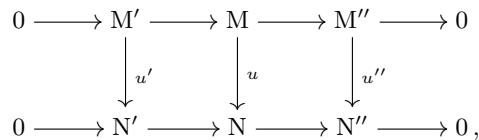
\includegraphics[keepaspectratio]{images/part002_92bb4337.jpg}}

其中第一行（相应地，第二行）是 Z{[}G{]}-模（相应地，Z{[}H{]}-模）的一个正合列，且 \(u', u, u''\) 与 \(\varphi\) 相容。证明图

\[
\begin{array}{l} \dots \longrightarrow \mathrm{H} ^ {n} (\mathrm{G}, \mathrm{M} ^ {\prime}) \longrightarrow \mathrm{H} ^ {n} (\mathrm{G}, \mathrm{M}) \longrightarrow \mathrm{H} ^ {n} (\mathrm{G}, \mathrm{M} ^ {\prime \prime}) \longrightarrow \mathrm{H} ^ {n + 1} (\mathrm{G}, \mathrm{M} ^ {\prime}) \longrightarrow \dots \\ \Biggl \downarrow_ {\mathrm{H} ^ {n} (\varphi , u ^ {\prime})} \qquad \Biggl \downarrow_ {\mathrm{H} ^ {n} (\varphi , u)} \qquad \Biggl \downarrow_ {\mathrm{H} ^ {n} (\varphi , u ^ {\prime \prime})} \qquad \Biggl \downarrow_ {\mathrm{H} ^ {n + 1} (\varphi , u)} \\ \dots \longrightarrow \mathrm{H} ^ {n} (\mathrm{H}, \mathrm{N} ^ {\prime}) \longrightarrow \mathrm{H} ^ {n} (\mathrm{H}, \mathrm{N}) \longrightarrow \mathrm{H} ^ {n} (\mathrm{H}, \mathrm{N} ^ {\prime \prime}) \longrightarrow \mathrm{H} ^ {n + 1} (\mathrm{H}, \mathrm{N} ^ {\prime}) \longrightarrow \dots \end{array}
\]

（其水平各行是习题 1, c) 中定义的长正合列）是交换的。

\begin{enumerate}
\def\labelenumi{\alph{enumi})}
\setcounter{enumi}{3}
\item
  例：若 H = G，则映射 u 与 \(Id_{G}\) 相容当且仅当它是 Z{[}G{]}-线性的，且我们有 \(\mathrm{H}^{n}(\mathrm{Id}_{\mathrm{G}}, u) = \mathrm{H}^{n}(\mathrm{G}, u)\)。若 N 等于 M（赋予一个 Z{[}G{]}-模结构，即由 \(\varphi\) 诱导的那一个），则同态 \(\varphi\) 与 \(1_{M}\) 相容；我们用 \(\operatorname{Res}^{q} : \mathrm{H}^{q}(\mathrm{G}, \mathrm{M}) \to \mathrm{H}^{q}(\mathrm{H}, \mathrm{M})\) 表示同态 \(\mathrm{H}^{q}(\varphi, 1_{\mathrm{M}})\)（“限制同态”）。
\item
  设 H 是 G 的一个正规子群，并设 \(M^{H}\) 是 M 中在 H 下不变的元素所成的子群（赋予由 G 的作用通过取商而诱导的 G/H 的作用）。典范满射 \(p: G \rightarrow G/H\) 与典范单射 \(j: M^{H} \rightarrow M\) 是相容的；我们用 \(\operatorname{Inf}^{q}: \operatorname{H}^{q}(\operatorname{G}/\operatorname{H}, \operatorname{M}^{\operatorname{H}}) \to \operatorname{H}^{q}(\operatorname{G}, \operatorname{M})\) 表示同态 \(\operatorname{H}^{q}(p, j)\)（“膨胀同态”）。证明序列
\end{enumerate}

\[
0 \to \mathrm{H} ^ {1} (\mathrm{G} / \mathrm{H}, \mathrm{M} ^ {\mathrm{H}}) \xrightarrow {\operatorname{Inf} ^ {1}} \mathrm{H} ^ {1} (\mathrm{G}, \mathrm{M}) \xrightarrow {\operatorname{Res} ^ {1}} \mathrm{H} ^ {1} (\mathrm{H}, \mathrm{M})
\]

是正合的。此外，若 \(\mathrm{H}^1 (\mathrm{H},\mathrm{M})\) 为零，则序列

\[
0 \to \mathrm{H} ^ {2} (\mathrm{G} / \mathrm{H}, \mathrm{M} ^ {\mathrm{H}}) \xrightarrow {\operatorname{Inf} ^ {2}} \mathrm{H} ^ {2} (\mathrm{G}, \mathrm{M}) \xrightarrow {\operatorname{Res} ^ {2}} \mathrm{H} ^ {2} (\mathrm{H}, \mathrm{M})
\]

是正合的。

¶ 3) 设 G 是一个群，M 是一个 Z{[}G{]}-模。让 G 作用在 C \(^{1}\) (G,M) 上，其作法是把 \((g,f)\in\mathrm{G}\times\mathrm{C}^{1}(\mathrm{G},\mathrm{M})\) 映为 G 上的函数 \(h\mapsto gf(g^{-1}h)\)。回顾（I, §6, 第 149 页，习题 8），M 上的一个 G-平均是一个 Z{[}G{]}-线性映射 \(\mu:C^{1}(\mathrm{G},\mathrm{M})\to\mathrm{M}\)，它满足 \(\mu(c_{x})=x\)，其中 \(c_{x}\) 表示取值 \(x\in\mathrm{M}\) 的常值函数。

\begin{enumerate}
\def\labelenumi{\alph{enumi})}
\item
  证明若 M 容许一个 G-平均，则 \(\mathrm{H}^{n}(\mathrm{G},\mathrm{M})\) 为零（对 \(n \geqslant 1\)）。（对 \(q \geqslant 1\)，设 \(h^{q}: \mathrm{C}^{q}(\mathrm{G},\mathrm{M}) \to \mathrm{C}^{q-1}(\mathrm{G},\mathrm{M})\) 是如下同态：对 G 中的 \(g_{1}, \ldots, g_{q-1}\) 与 \(c \in \mathrm{C}^{q}(\mathrm{G}, \mathrm{M})\)，把 \(h^{q}(c)(g_{1}, \ldots, g_{q-1})\) 定义为 \(\mu\) 作用于函数 \(g \mapsto c(g_{1}, \ldots, g_{q-1}, (g_{1} \cdots g_{q-1})^{-1}g)\) 所得的像。证明等式 \(h^{q+1} \circ d^{q} + d^{q-1} \circ h^{q} = 1_{\mathrm{C}^{q}(\mathrm{G}, \mathrm{M})}\)。
\item
  设 A 是一个交换群；用 \(\mathcal{F}(\mathrm{G},\mathrm{A})\) 表示从 G 到 A 的映射所成的群（赋予由 \({}^{g}f(h)=f(hg)\)（对 G 中的 g, h 与 \(\mathcal{F}(\mathrm{G},\mathrm{A})\) 中的 f）定义的 G 的作用）。对从 G 到 \(\mathcal{F}(\mathrm{G},\mathrm{A})\) 的任何映射 c，用 \(\mu(c)\) 表示从 G 到 A 的映射 \(g\mapsto c(g^{-1})(g)\)。证明 \(\mu\) 是 \(\mathcal{F}(\mathrm{G},\mathrm{A})\) 上的一个 G-平均；因此我们有 \(\mathrm{H}^{q}(\mathrm{G},\mathcal{F}(\mathrm{G},\mathrm{A}))=0\)（对 \(q\geqslant1\)）。
\item
  设 \(j: M \to \mathcal{F}(G, M)\) 是把 M 的元素 m 映为函数 \(g \mapsto gm\) 的映射，并设 \(M'\) 是它的余核。证明 j 是单射且是 Z{[}G{]}-线性的。由此推出同态 \(\partial^{q}: H^{q}(G, M') \to H^{q+1}(G, M)\) 是双射（对 \(q \geqslant 1\)）。
\item
  设 L 是交换域 K 的一个有限伽罗瓦扩张，并设 G 是它的伽罗瓦群。由 b) 与正规基定理（V, §10, No.~9, 第 73 页）推出，群 \(\mathrm{H}^{n}(\mathrm{G},\mathrm{L})\) 为零（对 \(n \geqslant 1\)）。
\end{enumerate}

¶ 4) 设 G 是一个群，H 是 G 的一个子群。对任何 Z{[}H{]}-模 N，用 \(\widetilde{N}\) 表示群 \(\operatorname{Hom}_{\mathbf{Z}[H]}(\mathbf{Z}[G], N)\)（赋予由 Z{[}G{]} 上的右 Z{[}G{]}-模结构诱导的一个 Z{[}G{]}-模结构）。

\begin{enumerate}
\def\labelenumi{\alph{enumi})}
\item
  证明 \(\widetilde{\mathbf{N}}\) 可与一个 \(\mathbf{Z}[\mathrm{G}]\)-子模等同起来，即 \(\mathcal{F}(\mathrm{G},\mathrm{N})\)（习题 3）中由映射 \(f\) 所组成的、满足 \(f(hg) = hf(g)\)（对每个 \(h\in \mathrm{H}\) 与每个 \(g\in \mathrm{G}\)）的那个子模。若 \(\mathrm{A}\) 是一个交换群，则 \(\mathbf{Z}[\mathrm{G}]\)-模 \(\widetilde{\mathcal{F}(\mathrm{H},\mathrm{A})}\) 典范同构于 \(\mathcal{F}(\mathrm{G},\mathrm{A})\)。
\item
  设 \(0 \rightarrow N' \stackrel{i}{\rightarrow} N \stackrel{p}{\rightarrow} N'' \rightarrow 0\) 是 Z{[}H{]}-模的一个正合列；序列
\end{enumerate}

\[
0 \longrightarrow \widetilde {\mathrm{N}} ^ {\prime} \xrightarrow {\operatorname{Hom} (1 , i)} \widetilde {\mathrm{N}} \xrightarrow {\operatorname{Hom} (1 , p)} \widetilde {\mathrm{N}} ^ {\prime \prime} \longrightarrow 0
\]

是正合的（注意 \(\mathbf{Z}[\mathrm{H}]\)-模 \(\mathbf{Z}[\mathrm{G}]\) 是自由的）。

\begin{enumerate}
\def\labelenumi{\alph{enumi})}
\setcounter{enumi}{2}
\tightlist
\item
  设 \(u_{N} : \widetilde{N} \to N\) 是映射 \(f \mapsto f(1)\)；它与典范单射 \(i : H \to G\) 相容（习题 2）。证明同态
\end{enumerate}

\[
\mathrm{H} ^ {q} (i, u _ {\mathrm{N}}): \mathrm{H} ^ {q} (\mathrm{G}, \widetilde {\mathrm{N}}) \to \mathrm{H} ^ {q} (\mathrm{H}, \mathrm{N})
\]

对每个 \(q \geqslant 0\) 是双射（先处理 q = 0 的情形，然后利用上述结果、习题 3, c) 以及习题 2, c)，对 q 作归纳法推理）。

\begin{enumerate}
\def\labelenumi{\alph{enumi})}
\setcounter{enumi}{3}
\item
  假设 H 在 G 中有有限指标 n。设 M 是一个 Z{[}G{]}-模，我们通过限制标量把它看作一个 Z{[}H{]}-模。设 \(f \in \widetilde{M}\)；元素 \(g^{-1}f(g)\) 只依赖于 g 的右陪集 Hg。令 \(\pi(f) = \sum_{Hg \in H \setminus G} g^{-1}f(g)\)。证明 \(\pi\) 是一个 Z{[}G{]}-线性同态（从 \(\widetilde{M}\) 到 M 的）。对任何整数 \(q \geqslant 0\)，用 \(\operatorname{Cor}^{q}: \mathrm{H}^{q}(\mathrm{H}, \mathrm{M}) \to \mathrm{H}^{q}(\mathrm{G}, \mathrm{M})\) 表示同态 \(\mathrm{H}^{q}(\pi) \circ \mathrm{H}^{q}(i, u_{\mathrm{M}})^{-1}\)（“余限制同态”）。
\item
  证明自同态 \(Cor^{q} \circ Res^{q}\)（\(H^{q}(G, M)\) 的）是乘以 n 的映射（先处理 q = 0 的情形，然后按 c) 的证明中的做法处理一般情形）。
\item
  假设 G 是有限的；证明对每个 Z{[}G{]}-模 M 与每个整数 \(q \geqslant 1\)，群 \(\mathrm{H}^{q}(\mathrm{G}, \mathrm{M})\) 被 G 的阶零化。
\end{enumerate}

\begin{enumerate}
\def\labelenumi{\arabic{enumi})}
\setcounter{enumi}{4}
\tightlist
\item
  设 G 是一个群，M 是一个不一定交换的群（赋予一个同态 \(\varphi: G \to \text{Aut}(M)\)）；对 \(g \in G\) 与 \(m \in M\)，令 \(^{g}m = \varphi(g)(m)\)。用 \(H^{0}(G, M)\) 表示 M 中被 G 的作用固定的元素所成的子群；它的单位元素称为 \(H^{0}(G, M)\) 的标记元素或特异元素。设 \(Z^{1}(G, M)\) 是映射 \(c: G \to M\) 所成之集，其中 c 满足 \(c(gh) = c(g)^{g}c(h)\)（对 G 中的 g, h）。对 \(c \in Z^{1}(G, M)\) 与 \(m \in M\)，映射 \(g \mapsto mc(g)(^g m)^{-1}\) 属于 \(Z^{1}(G, M)\)；这就定义了群 M 在 \(Z^{1}(G, M)\) 上的一个作用。商集记作 \(H^{1}(G, M)\)；它带有一个标记元素，即取值 1 的常值映射的类。若 M 是交换的，则集合 \(H^{1}(G, M)\) 与习题 1 中定义的那个重合。
\end{enumerate}

\begin{enumerate}
\def\labelenumi{\alph{enumi})}
\item
  设 N 是另一个赋予 G 的作用的群，并设 \(u: M \to N\) 是一个与 G 的作用相容的群同态。对 i = 0, 1，定义同态 \(\mathrm{H}^{i}(u): \mathrm{H}^{i}(\mathrm{G}, \mathrm{M}) \to \mathrm{H}^{i}(\mathrm{G}, \mathrm{N})\)，它们把 \(\mathrm{H}^{i}(\mathrm{G}, \mathrm{M})\) 的标记元素映为 \(\mathrm{H}^{i}(\mathrm{G}, \mathrm{N})\) 的标记元素。
\item
  设 \(0 \to M' \xrightarrow{\iota} M \xrightarrow{\pi} M'' \to 0\) 是带 G 中算子的群的一个正合列。设 \(x'' \in \mathrm{H}^0(\mathrm{G}, \mathrm{M}'')\)，并设 x 是 M 的一个元素，使得 \(\pi(x) = x''\)。证明存在一个元素 \(c' \in \mathrm{Z}^1(\mathrm{G}, \mathrm{M}')\)，使得 \(\iota \circ c'(g) = g^{-1}c(g)\)（对每个 \(g \in G\)），并且 \(c'\) 在 \(\mathrm{H}^1(\mathrm{G}, \mathrm{M}')\) 中的类只依赖于 \(x''\)；我们把该类记作 \(\partial(x'')\)。证明序列
\end{enumerate}

\[
0 \to \mathrm{H} ^ {0} (\mathrm{G}, \mathrm{M} ^ {\prime}) \xrightarrow {\mathrm{H} ^ {0} (\iota)} \mathrm{H} ^ {0} (\mathrm{G}, \mathrm{M}) \xrightarrow {\mathrm{H} ^ {0} (\pi)} \mathrm{H} ^ {0} (\mathrm{G}, \mathrm{M} ^ {\prime \prime}) \xrightarrow {\partial}
\]

\[
\mathrm{H} ^ {1} (\mathrm{G}, \mathrm{M} ^ {\prime}) \xrightarrow {\mathrm{H} ^ {1} (\iota)} \mathrm{H} ^ {1} (\mathrm{G}, \mathrm{M}) \xrightarrow {\mathrm{H} ^ {1} (\pi)} \mathrm{H} ^ {1} (\mathrm{G}, \mathrm{M} ^ {\prime \prime})
\]

是正合的（映射序列 \(G \xrightarrow{i} F \xrightarrow{p} E\)（其中集合 E 带有一个标记元素 e）称为在 F 处正合，如果 \(\operatorname{Im}(i) = p^{-1}(e)\)）。

\begin{enumerate}
\def\labelenumi{\alph{enumi})}
\setcounter{enumi}{2}
\item
  此外，假设 \(M'\) 包含在 M 的中心内。构造一个映射 \(\partial^{1}: H^{1}(G, M'') \to H^{2}(G, M')\)，使得单位元素在 \(\partial^{1}\) 下的逆像是 \(H^{1}(\pi)\) 的像。再定义群 \(H^{1}(G, M')\) 在集合 \(H^{1}(G, M)\) 上的一个作用，使得两个元素在这个作用下共轭当且仅当它们在 \(H^{1}(\pi)\) 下有相同的像。
\item
  设 K 是一个交换域，L 是 K 的一个有限伽罗瓦扩张（伽罗瓦群为 G），n 是一个整数。让 G 作用在群 \(\mathbf{GL}_{n}(\mathrm{L})\) 上，其作法是令 \(\sigma A = (\sigma(a_{ij}))\)（对 \(\sigma \in G\) 与 \(A = (a_{ij}) \in \mathbf{GL}_{n}(\mathrm{L})\)）。由 V, §10, No.~5, 第 64 页，命题 9 推出，集合 \(\mathrm{H}^{1}(\mathrm{G}, \mathbf{GL}_{n}(\mathrm{L}))\) 只含一个元素（“希尔伯特定理 90”）。
\end{enumerate}

¶ 6) 设 L 是交换域 K 的一个有限伽罗瓦扩张（伽罗瓦群为 G）。设 V 与 V' 是 K-向量空间，w（相应地，w'）是 V（相应地，V'）上一个 \((p,q)\) 型张量。从 \((V,w)\) 到 \((V',w')\) 的一个 L-同构是一个 L-线性同构 \(u:V_{(L)}\to V_{(L)}'\)，使得 \(u^{\otimes p}\otimes(^{t}u^{-1})^{\otimes q}\) 把 w 的像映为 \(w'\) 的像。我们用 \(\operatorname{Aut}_{\mathrm{L}}(\mathrm{V},w)\) 表示 \((\mathrm{V},w)\) 的 L-自同构所成的群，G 在其上通过 \(\sigma\varphi=(1_{\mathrm{V}}\otimes\sigma)\circ\varphi\circ(1_{\mathrm{V}}\otimes\sigma)^{-1}\) 作用。

\begin{enumerate}
\def\labelenumi{\alph{enumi})}
\item
  设 u 是从 \((\mathrm{V}, w)\) 到 \((\mathrm{V}^{\prime}, w^{\prime})\) 的一个 L-同构，\(\sigma\) 是 G 的一个元素；映射 \(\sigma u = (1_{\mathrm{V}^{\prime}} \otimes \sigma) \circ u \circ (1_{\mathrm{V}} \otimes \sigma)^{-1}\) 是从 \((\mathrm{V}, w)\) 到 \((\mathrm{V}^{\prime}, w^{\prime})\) 的一个 L-同构，从而 \(c(\sigma) = u^{-1} \circ \sigma u\) 是 \(\operatorname{Aut}_{\mathrm{L}}(\mathrm{V}, w)\) 的一个元素。证明映射 \(c : G \to \operatorname{Aut}_{\mathrm{L}}(\mathrm{V}, w)\) 属于 \(Z^{1}(\mathrm{G}, \operatorname{Aut}_{\mathrm{L}}(\mathrm{V}, w))\)，并且它的类 \(\theta(\mathrm{V}^{\prime}, w^{\prime})\)（在 \(H^{1}(\mathrm{G}, \operatorname{Aut}_{\mathrm{L}}(\mathrm{V}, w))\) 中的）不依赖于 u 的选取。
\item
  证明映射 \((\mathrm{V}^{\prime},t^{\prime})\mapsto\theta(\mathrm{V}^{\prime},t^{\prime})\) 定义了一个双射（从偶 \((\mathrm{V}^{\prime},w^{\prime})\)（L-同构于 \((\mathrm{V},w)\) 的）的 K-同构类所成之集到集合 \(\mathrm{H}^{1}(\mathrm{G},\mathrm{Aut}_{\mathrm{L}}(\mathrm{V},w))\) 的）。（设 c 是 \(\mathrm{Z}^{1}(\mathrm{G},\mathrm{Aut}_{\mathrm{L}}(\mathrm{V},w))\) 的一个元素，由习题 5, d) 推出 \(\mathrm{V}_{(\mathrm{L})}\) 的一个 L-自同构 f，使得 \(c(\sigma)=f^{-1}\circ^{\sigma}f\)。证明 w 在由 f 诱导的自同构下的像 \(w^{\prime}\) 在 K 上是有理的，并考虑偶 \((\mathrm{V},w^{\prime}).\)）
\end{enumerate}

* c) 例：集合 \(\mathrm{H}^1 (\mathrm{G},\mathbf{Sp}_{2n}(\mathrm{L}))\) 只含一个元素。若 Q 是 K 上的一个二次型，则集合 \(\mathrm{H}^1 (\mathrm{G},\mathbf{O}(\mathrm{Q}_{(\mathrm{L})}))\) 可与在 L 上等价于 Q 的 K 上二次型的等价类所成之集等同起来。*

\(d\) ) 设 A 是一个 K-代数，M 是 L-代数 \(\mathrm{A}_{(\mathrm{L})}\) 的自同构群（赋予上面定义的 G 的作用）。\(b\)）中的构造定义了一个双射，从偶 \((\mathrm{B},u)\)（其中 B 是一个 K-代数，而 \(u\) 是从 \(\mathrm{B}_{(\mathrm{L})}\) 到 \(\mathrm{A}_{(\mathrm{L})}\) 的一个同构）的同构类所成之集到集合 \(Z^{1}(\mathrm{G},\mathrm{M})\)。逆双射把元素 \(c\)（属于 \(Z^{1}(\mathrm{G},\mathrm{M})\)）映为 \(\mathrm{A}_{(\mathrm{L})}\) 中由元素 \(a\)（满足 \(c(\sigma)(\sigma(a)) = a\)，对每个 \(\sigma \in \mathrm{G}\)）所成的 K-子代数。

\begin{enumerate}
\def\labelenumi{\arabic{enumi})}
\setcounter{enumi}{6}
\tightlist
\item
  设 L 是 K 的一个扩张。对任何整数 \(n \geqslant 1\)，用 \(\mathcal{A}_{n}(\mathrm{L}/\mathrm{K})\) 表示被 L 分裂的、次数为 \(n^{2}\) 的中心单 K-代数的同构类所成之集。
\end{enumerate}

\begin{enumerate}
\def\labelenumi{\alph{enumi})}
\item
  证明核 \(\mathrm{Br}(\mathrm{L} / \mathrm{K})\)（典范同态 \(\mathrm{Br}(\mathrm{K})\to \mathrm{Br}(\mathrm{L})\) 的）同构于集合 \(\mathcal{A}_n(\mathrm{L} / \mathrm{K})\) 的正向极限；给出一个映射系。b) 从现在起假设 L 是 K 的一个有限伽罗瓦扩张（伽罗瓦群为 G）。由习题 6 推出一个双射 \(\theta_{n}:\mathcal{A}_{n}(\mathrm{L} / \mathrm{K})\to \mathrm{H}^{1}(\mathrm{G},\mathbf{PGL}_{n}(\mathrm{L}))\)。
\item
  用 \(\partial_n: \mathrm{H}^1(\mathrm{G}, \mathbf{PGL}_n(\mathrm{L})) \to \mathrm{H}^2(\mathrm{G}, \mathrm{L}^*)\) 表示由正合列 \(1 \to \mathrm{L}^* \to \mathbf{GL}_n(\mathrm{L}) \to \mathbf{PGL}_n(\mathrm{L}) \to 1\)（习题 5, c)）诱导的映射，并用 \(\delta_n: \mathcal{A}_n(\mathrm{L/K}) \to \mathrm{H}^2(\mathrm{G}, \mathrm{L}^*)\) 表示映射 \(\partial_n \circ \theta_n\)。若 \(\mathrm{A} \in \mathcal{A}_n(\mathrm{L/K})\)，则我们有 \(\delta_n(\mathrm{A}) = 0\) 当且仅当 \(\mathrm{A}\) 是 \(\mathrm{K}\) 上的一个矩阵代数；若 \(\mathrm{A} \in \mathcal{A}_p(\mathrm{L/K})\) 且 \(\mathrm{B} \in \mathcal{A}_q(\mathrm{L/K})\)，则我们有 \(\delta_{pq}(\mathrm{A} \otimes_{\mathrm{K}} \mathrm{B}) = \delta_p(\mathrm{A}) + \delta_q(\mathrm{B})\)。通过取正向极限，推出一个单群同态 \(\delta_{\mathrm{L/K}}: \mathrm{Br}(\mathrm{L/K}) \to \mathrm{H}^2(\mathrm{G}, \mathrm{L}^*)\)。d) 证明 \(\partial_n\) 是满射（对 \(n = \operatorname{Card}(\mathrm{G})\)）。（设 \(c: \mathrm{G} \times \mathrm{G} \to \mathrm{L}^*\) 是 \(\mathrm{Z}^2(\mathrm{G}, \mathrm{L}^*)\) 的一个元素。对每个 \(\sigma \in \mathrm{G}\)，考虑自同态 \(u(\sigma)\)（\(\mathrm{L}^{\mathrm{G}}\) 的），它把 \(e_\tau\) 映为 \(c(\sigma, \tau)e_{\sigma\tau}\)（对每个 \(\tau \in \mathrm{G}\)），并确定 \(u(\sigma)^{\sigma}u(\tau)u(\sigma\tau)^{-1}\)。）
\item
  比较 \(\delta_{\mathrm{L / K}}\) 与 \(\Phi_{\mathrm{L / K}}\)。
\item
  证明群 \(\mathrm{Br}(\mathrm{K})\) 可与群 \(\left(\mathrm{H}^{2}(\mathrm{Gal}(\mathrm{L}/\mathrm{K}),\mathrm{L}^{*})\right)\) 的正向系统（关于 K 的包含在一个固定代数闭包中的有限伽罗瓦扩张所成的集合（按包含排序）取的）的极限等同起来，其中这些群之间的同态是（单的）膨胀同态。g) 设 F 是包含在 L 中的 K 的一个扩张，并设 \(\Gamma\) 是 G 中保持 F 不变的子群。证明下面的图是交换的：
\end{enumerate}

\[
\begin{array}{c} \operatorname{Br} (\mathrm{L} / \mathrm{K}) \xrightarrow {r _ {\mathrm{F} / \mathrm{K}}} \operatorname{Br} (\mathrm{F} / \mathrm{L}) \\ \Biggl \downarrow_ {\delta_ {\mathrm{L} / \mathrm{K}}} \qquad \qquad \qquad \qquad \Biggl \downarrow_ {\delta_ {\mathrm{F} / \mathrm{L}}} \\ \operatorname{H} ^ {2} (\operatorname{G}, \operatorname{L} ^ {*}) \xrightarrow {\operatorname{Res} ^ {2}} \operatorname{H} ^ {2} (\Gamma , \operatorname{L} ^ {*}). \end{array}
\]

由此推出一个从 \(\mathrm{Br}(\mathrm{F}/\mathrm{K})\) 到同态 \(\mathrm{Res}^{2}:\mathrm{H}^{2}(\mathrm{G},\mathrm{L}^{*})\to\mathrm{H}^{2}(\Gamma,\mathrm{L}^{*})\) 的核的典范同构。

\begin{enumerate}
\def\labelenumi{\arabic{enumi})}
\setcounter{enumi}{7}
\item
  设 L 是 K 的一个扩张。假设 K 的特征为 p \textgreater{} 0 且 \(L = K^{1/p}\)。证明群 \(\mathrm{Br}(\mathrm{L}/\mathrm{K})\) 等于 \(\mathrm{Br}(\mathrm{K})\) 中乘以 p 的同态的核（注意若 N 是 K 的一个有限伽罗瓦扩张，则 \(N^{1/p}\) 是 L 的一个伽罗瓦扩张，且伽罗瓦群相同）。
\item
  设 G 是一个有限群，M 是一个 Z{[}G{]}-模。用 \(N_{G}\) 表示从 M 到 M 的同态 \(m \mapsto \sum_{g} gm\)；它的像包含在 M 的由不变元素所成的子模 \(M^{G}\) 中。设 \(\mathrm{T}_{\mathrm{G}}(\mathrm{M})\) 是商群 \(\mathrm{M}^{\mathrm{G}}/\mathrm{N}_{\mathrm{G}}(\mathrm{M})\)。a) 设 \(c \in \mathrm{Z}^{2}(\mathrm{G}, \mathrm{M})\)。证明元素 \(\sum_{h} c(h, g)\) 属于 \(M^{G}\)；我们把它在 \(\mathrm{T}_{\mathrm{G}}(\mathrm{M})\) 中的类记作 \(\theta_{c}(g)\)。证明 \(\theta_{c}\) 是从 G 到 \(\mathrm{T}_{\mathrm{G}}(\mathrm{M})\) 的一个同态，且当 \(c \in \mathrm{B}^{2}(\mathrm{G}, \mathrm{M})\) 时它为零。由此推出一个同态 \(\theta_{\mathrm{M}} : \mathrm{H}^{2}(\mathrm{G}, \mathrm{M}) \to \mathrm{Hom}(\mathrm{G}, \mathrm{T}_{\mathrm{G}}(\mathrm{M}))\)。
\end{enumerate}

\begin{enumerate}
\def\labelenumi{\alph{enumi})}
\setcounter{enumi}{1}
\tightlist
\item
  设 \(u: M \to N\) 是 Z{[}G{]}-模的一个同态，并设 \(\widetilde{u}: T_{G}(M) \to T_{G}(N)\) 是由 u 诱导的同态。证明我们有 \(\theta_{\mathrm{N}} \circ \mathrm{H}^{2}(u) = \mathrm{Hom}(1_{\mathrm{G}}, \widetilde{u}) \circ \theta_{\mathrm{M}}\)。c) 从现在起假设 G 是循环的；设 \(\sigma\) 是 G 的一个生成元，并用 n 表示它的阶。~设 \(\chi \in \mathrm{Hom}(G, \mathbf{Z}/n\mathbf{Z})\) 是把 \(\sigma\) 映为 1 的类的同态，并设 \(\lambda \in H^{2}(G, \mathbf{Z})\) 是它在伴随于正合列 \(0 \to Z \to Z \to Z/nZ \to 0\) 的连接同态下的像。证明 \(\lambda\) 是元素 \(\varepsilon \in Z^{2}(G, \mathbf{Z})\) 的类，该元素满足：对 \(0 \leqslant p < n\) 与 \(0 \leqslant q < n\)，像 \(\varepsilon(\sigma^{p}, \sigma^{q})\) 当 \(p + q < n\) 时等于 0，当 \(p + q \geqslant n\) 时等于 1。对 \(m \in M^{G}\)，用 \(h_{m}\) 表示一个 Z{[}G{]}-线性映射（从 Z 到 M 的），它满足 \(h_{m}(1) = m\)。证明 \(H^{2}(h_{m})(\lambda)\) 在 \(\theta_{M}\) 下的像等于 m 的类，从而 \(\theta_{M}\) 是满射。
\end{enumerate}

\(d\) ) 证明 \(\theta_{\mathrm{M}}\) 是一个同构。（设 \(c\in \mathbf{Z}^2 (\mathrm{G},\mathrm{M})\)。证明我们可以假设 \(c(g,1) = c(1,g) = 1\)（对每个 \(g\in \mathrm{G}\)），并确定 \(d^1\) 在元素 \(b\) 与 \(a_{m}\) \((m\in \mathrm{M})\)（\(\mathrm{C}^1 (\mathrm{G},\mathrm{M})\) 中的）处的像，这两个元素由 \(b(\sigma^{p}) = \sum_{i = 0}^{p - 1}c(\sigma^{i},\sigma)\) 与 \(a_{m}(\sigma^{p}) = \sum_{i = 0}^{p - 1}\sigma^{i}m.)\) 定义。）

\begin{enumerate}
\def\labelenumi{\arabic{enumi})}
\setcounter{enumi}{9}
\tightlist
\item
  \begin{enumerate}
  \def\labelenumii{\alph{enumii})}
  \tightlist
  \item
    设 L 是 K 的一个循环扩张。由习题 9 与 7 推出，群 Br(L/K) 与 \(K^{*}/N_{L/K}(L^{*})\) 是同构的。
  \end{enumerate}
\end{enumerate}

\begin{enumerate}
\def\labelenumi{\alph{enumi})}
\setcounter{enumi}{1}
\item
  假设 K 的每个有限次扩张 L 都是循环的，且范数映射 \(N_{L/K}: L^{*} \to K^{*}\) 是满射。证明每个中心为 K 的 K 上有限次体扩张都等于 K。
\item
  把前面的问题应用于有限域。
\end{enumerate}

\begin{enumerate}
\def\labelenumi{\arabic{enumi})}
\setcounter{enumi}{10}
\tightlist
\item
  设 L 是 K 的一个循环扩张（伽罗瓦群为 G），并设 \(\sigma\) 是 G 的一个生成元。习题 10 给出一个典范同构 \(\mathrm{Br}(\mathrm{L}/\mathrm{K}) \to \mathrm{K}^{*}/\mathrm{N}_{\mathrm{L}/\mathrm{K}}(\mathrm{L}^{*})\)，我们现在来明显地构造它的逆。
\end{enumerate}

设 \(\theta \in \mathrm{K}^*\)，并设 \(c_{\theta} \in \mathrm{Z}^{2}(\mathrm{G}, \mathrm{L}^{*})\) 是由 \(c_{\theta}(\sigma^{p}, \sigma^{q}) = \theta^{\varepsilon(p,q)}\) 定义的元素（习题 9, \(c\) )）。证明交叉乘积 A{[} \(\mathcal{E}\) , L{]}（L 与扩张 \(\mathcal{E}\)（同 \(c_{\theta}\) 相伴的）的）同构于 K-代数 L{[}X{]} \(_{\sigma}\)（VIII, 第 11 页）关于由中心元素 X \(^{n}\) - \(\theta\) 生成的（双边）理想所得的商。A \(_{\theta}\) 在 Br(L/K) 中的类通过上面定义的同构对应于 \(\theta\) 的类（ \(\text{mod } \mathrm{N}_{\mathrm{L/K}}(\mathrm{L}^{*})\) ）。

\begin{enumerate}
\def\labelenumi{\arabic{enumi})}
\setcounter{enumi}{11}
\tightlist
\item
  设 A 是一个交换环。给 Azumaya A-代数（VIII, 第 270 页，习题 8）的同构类所成之集赋予一个幺半群结构，其作法是令 \(\operatorname{cl}(S)\operatorname{cl}(T)=\operatorname{cl}(S\otimes_{A}T)\)。
\end{enumerate}

\begin{enumerate}
\def\labelenumi{\alph{enumi})}
\item
  证明关于 Morita 等价的商幺半群是一个交换群；我们把它记作 Br(A)，并称之为 A 的布饶尔群（当 A 是一个体时，这个定义与 VIII, 第 279 页给出的定义重合）。用 {[}S{]} 表示一个 Azumaya A-代数 S 在 Br(A) 中的类。Br(A) 的单位元素是 A 的类，而元素 {[}S{]} 的逆是 {[}S°{]}。
\item
  设 S 是一个 Azumaya A-代数。我们有 \([S] = [A]\) 当且仅当存在一个有限生成、投射、忠实的 A-模 P，使得 S 同构于 \(\operatorname{End}_{\mathrm{A}}(\mathrm{P})\)。
\item
  设 B 是一个交换 A-代数。定义一个群同态 \(r_{B/A} : \mathrm{Br}(A) \to \mathrm{Br}(B)\)，使得 \(r_{\mathrm{B/A}}([\mathrm{S}]) = [\mathrm{S}_{(\mathrm{B})}]\)（对每个 Azumaya A-代数 S）。我们把这个同态的核记作 \(\mathrm{Br(B/A)}\)。
\end{enumerate}

¶ 13) 设 A 是一个交换环，B 是一个交换 A-代数，G 是 A-代数 B 的自同构所成的一个有限群。假设 B 是一个有限生成、投射、忠实的 A-模，且 A-线性同态 \(\psi : \mathrm{B} \otimes_{\mathrm{A}} \mathrm{B} \to \mathrm{B}^{\mathrm{G}}\)（由 \(\psi(b \otimes b') = (\sigma(b)b')_{\sigma \in \mathrm{G}}\) 定义的）是双射。

\begin{enumerate}
\def\labelenumi{\alph{enumi})}
\item
  设 N 是一个 B-模（赋予一个同态 \(\sigma \mapsto u_{\sigma}\)（从 G 到 \(\mathrm{Aut}_{\mathrm{A}}(\mathrm{N})\) 的），它满足 \(u_{\sigma}(bx) = \sigma(b)u_{\sigma}(x)\)（对 \(\sigma \in \mathrm{G}\)、\(b \in \mathrm{B}\)、\(x \in \mathrm{N}\)））。设 M 是 N 中由元素 \(x\)（满足 \(u_{\sigma}(x) = x\)，对每个 \(\sigma \in \mathrm{G}\)）所成的 A-子模。证明典范 B-同态 \(\mathrm{B} \otimes_{\mathrm{A}} \mathrm{M} \to \mathrm{N}\) 是双射（利用 VIII, 第 270 页的习题 7, \(d\) ) 化归为 B 是积代数 \(\mathrm{A}^{\mathrm{G}}\)（G 通过置换诸因子在其上作用）的情形）。
\item
  设 S 是一个 A-代数，M 是 B-代数 \(\mathrm{S}_{(\mathrm{B})}\) 的自同构群，G 在其上通过 \(\sigma\varphi = (\mathrm{Id}_{\mathrm{S}} \otimes \sigma) \circ \varphi \circ (\mathrm{Id}_{\mathrm{S}} \otimes \sigma)^{-1}\) 作用。推广习题 6 的构造，以定义一个双射，从偶 \((T,u)\)（其中 T 是一个 A-代数，而 u 是从 \(T_{(B)}\) 到 \(S_{(B)}\) 的一个同构）的同构类所成之集到集合 \(Z^{1}(G,M)\)，并定义一个双射，从使得 B-代数 \(T_{(B)}\) 与 \(S_{(B)}\) 同构的 A-代数 T 的同构类所成之集到 \(H^{1}(G,M)\)。
\item
  从现在起假设每个投射 B-模都是自由的。修改习题 8 的推理以构造一个同构 \(\theta : \mathrm{Br}(\mathrm{B} / \mathrm{A}) \to \mathrm{H}^2(\mathrm{G}, \mathrm{B}^*)\)。
\end{enumerate}

¶ 14) 设 A 是一个诺特交换局部环，m 是它的极大理想，\(\kappa\) 是体 A/m，而 S 是 A 上的一个 Azumaya 代数。

\begin{enumerate}
\def\labelenumi{\alph{enumi})}
\item
  设 \(e\) 是 S 中的一个幂等元，它在 S/mS 中的像是一个不可分解幂等元。由中山引理（参看 VIII, 第 168 页，习题 16）推出，典范同态 \(S \to \mathrm{End}_{\mathrm{A}}(Se)\) 是双射。
\item
  假设 m 是幂零的 \(^{*}\)（或者更一般地，A 对 m-adic 拓扑是完备的） \(^{*}\) 。证明同态 \(r_{\kappa/A}: \mathrm{Br}(A) \to \mathrm{Br}(\kappa)\) 是单射。
\end{enumerate}

* \(c\) ) 从现在起假设 A 是完备的。设 L 是 \(\kappa\) 的一个有限次可分扩张，且是 \(\kappa\)-代数 S/mS 的一个分裂域。设 \(x\) 是 L 的一个本原元素，\(f\) 是它的极小多项式，F 是 A{[}X{]} 中的一个首一多项式（它在 \(\kappa\) {[}X{]} 中的像是 \(f\)），并设 B = A{[}X{]}/(F)。证明 B 是一个局部 A-代数（作为 A-模是自由且有限生成的），其极大理想为 mB，剩余域同构于 L；B-代数 S \(_{(B)}\) 同构于一个矩阵代数。

\(d\) ) 此外，假设 L 是 \(\kappa\) 的一个伽罗瓦扩张（伽罗瓦群为 G）。证明 G 在 L 上的作用可提升为在 A-代数 B 上的一个作用（设 \(G'\) 是这个代数的自同构群；由 Hensel 引理（《交换代数》，III, §4, No.~3, 第 215 页，定理 1）推出，自然同态 \(G' \to G\) 是双射）。由中山引理推出，习题 13 中定义的同态 \(\psi : B \otimes_A B \to B^G\) 是双射。

\begin{enumerate}
\def\labelenumi{\alph{enumi})}
\setcounter{enumi}{4}
\item
  证明同态 \(\mathrm{H}^{q}(\pi):\mathrm{H}^{q}(\mathrm{G},\mathrm{B}^{*})\to\mathrm{H}^{q}(\mathrm{G},\mathrm{L}^{*})\) 是双射（对每个 \(q\geqslant1\)）。（对 \(i\geqslant1\)，设 \(U^{i}\) 是 \(B^{*}\) 中满足 \(b\equiv1\) (mod \(m^{i}B\) ) 的元素 b 所成的子群。注意 Z{[}G{]}-模 \(U^{i}/U^{i+1}\) 同构于 \(m^{i}B/m^{i+1}B\)，从而同构于 L 的一个幂，并由习题 5, d) 推出 \(\mathrm{H}^{q}(\mathrm{G},\mathrm{U}^{i}/\mathrm{U}^{i+1})\) 为零（对 \(q\geqslant1\)）。设 \(c\in\mathrm{Z}^{q}(\mathrm{G},\mathrm{U}^{1})\)。用归纳法构造一个序列 \((b_{n})\)，其中 \(b_{n}\in\mathrm{Z}^{q-1}(\mathrm{G},\mathrm{U}^{n})\)，使得 \(c-d^{q-1}(\sum_{i=1}^{n}b_{i})\) 属于 \(\mathrm{Z}^{q}(\mathrm{G},\mathrm{U}^{n+1})\)。由此得出 \(\mathrm{H}^{q}(\mathrm{G},\mathrm{U}^{1})\) 为零（对 \(q\geqslant1\)）。
\item
  由此得出，典范同态 \(\mathrm{Br}(B/A)\to \mathrm{Br}(L/\kappa)\) 与 \(\mathrm{Br}(A)\to \mathrm{Br}(\kappa)\) 都是双射。*
\end{enumerate}

\begin{enumerate}
\def\labelenumi{\arabic{enumi})}
\setcounter{enumi}{14}
\tightlist
\item
  *a) 设 A 是一个正则整环（AC, X, §4, n° 2, 第 55 页），K 是它的分式域。同态 \(r_{\mathrm{K / A}}: \mathrm{Br(A)} \to \mathrm{Br(K)}\) 是单射（VIII, 第 271 页，习题 11）。*
\end{enumerate}

\begin{enumerate}
\def\labelenumi{\alph{enumi})}
\setcounter{enumi}{1}
\tightlist
\item
  证明环 \(A = \mathbf{Q}[X, Y]/(X^{2} + Y^{2})\) 是一个整环；设 K 是它的分式域。设 H 是 Q 上 \((-1, 0, -1)\) 型的四元数代数，它是一个体（参看 III, §2, No.~5, 第 445 页）。证明以下 Azumaya
\end{enumerate}

A-代数 \(\mathrm{H}_{(\mathrm{A})}\) 在 \(\mathrm{Br}(\mathrm{A})\) 中的类不为零，但 \(\mathrm{H}_{(\mathrm{K})}\) 同构于 \(\mathbf{M}_{2}(\mathrm{K})\)，从而同态 \(r_{K/A}\) 不是单射（注意 K 包含一个平方为 -1 的元素）。

\begin{enumerate}
\def\labelenumi{\arabic{enumi})}
\setcounter{enumi}{15}
\tightlist
\item
  \begin{enumerate}
  \def\labelenumii{\alph{enumii})}
  \tightlist
  \item
    证明同态 \(r_{\mathrm{K[X]}/\mathrm{K}} : \mathrm{Br}(\mathrm{K}) \to \mathrm{Br}(\mathrm{K}[\mathrm{X}])\) 诱导一个从 \(\mathrm{Br}(\mathrm{K})\) 到 \(\mathrm{Br}(\mathrm{K}[\mathrm{X}])\) 的一个直因子的同构。
  \end{enumerate}
\end{enumerate}

\(^{*}b\) ) 假设体 K 是完满的。证明 \(r_{K[X]/K}\) 是一个同构（由曾定理（VIII, 第 360 页，习题 7）推出，\(\mathrm{Br}(\mathrm{K}[\mathrm{X}])\) 是诸群 \(\mathrm{Br}(\mathrm{L}[\mathrm{X}]/\mathrm{K}[\mathrm{X}])\) 的并，其中 L 取遍 K 的有限次伽罗瓦扩张，然后应用习题 13）。

\begin{enumerate}
\def\labelenumi{\alph{enumi})}
\setcounter{enumi}{2}
\tightlist
\item
  设 A 是一个正则 Q-代数且是一个整环。证明同态 \(r_{\mathrm{A[X]}/\mathrm{A}} : \mathrm{Br}(\mathrm{A}) \to \mathrm{Br}(\mathrm{A}[\mathrm{X}])\) 是双射（利用 b) 与习题 15 证明同态 \(\mathrm{Br}(\mathrm{A}[\mathrm{X}]) \to \mathrm{Br}(\mathrm{A})\)（由满射 \(\mathrm{P} \mapsto \mathrm{P}(0)\) 诱导的）是单射）。*
\end{enumerate}

\(d\) ) 假设 K 的特征为 \(p > 0\) 且不是完满的；设 \(\theta \in \mathrm{K} - \mathrm{K}^p\)。把 \(\mathrm{B} = \mathrm{K}[\mathrm{U}]\) 看作一个 K{[}X{]}-代数（通过同态 \(\rho : \mathrm{K}[\mathrm{X}] \to \mathrm{B}\)（由 \(\rho (\mathrm{X}) = \mathrm{U}^p - \mathrm{U}\) 确定的））。设 \(\sigma\) 是这个 K{[}X{]}-代数的满足 \(\sigma (\mathrm{U}) = \mathrm{U} + 1\) 的自同构，并设 S 是商 K{[}X{]}-代数（B{[}V{]}\(_{\sigma}\)（VIII, 第 11 页）关于双边理想 B(\(V^{p} - \theta\)) 的）。设 L 是一个 K{[}X{]}-代数，且是一个交换域。证明若方程 \(y^p - y = X\) 在 L 中有一个解，则 S\(_{(L)}\) 是 L 上的一个矩阵代数（设 L' = L{[}t{]}/(\(t^{p} - \theta\))；考虑同态 S → End\(_{\mathrm{L}}\) (L')，它把 V 映为 t 所定义的乘法 \(m_t\)，把 U 映为 \(m_y\) - D，其中 D 是 L' 的满足 D(t) = t 的 L-导子）。在相反的情形，S\(_{(L)}\) 是一个中心单 L-代数；它是一个矩阵代数当且仅当 \(\theta\) 是 L 的扩张 L{[}Y{]}/(\(Y^{p} - Y - X\)) 中某个元素的范数（应用习题 11）。

由此推出 S 是一个 Azumaya K{[}X{]}-代数，并且它在 \(\mathrm{Br}(\mathrm{K}[\mathrm{X}])\) 中的类不是来自 \(\mathrm{Br}(\mathrm{K})\) 的（取 \(L = K(X)\)）。

*17) 假设体 K 对一个离散赋值 \(v\)（设为赋值的）是完备的（参看 VIII, 第 272 页的习题 12）；用 A 表示 \(v\) 的环，用 \(\kappa\) 表示它的剩余域。同态 \(r_{\kappa / \mathrm{A}}: \mathrm{Br}(\mathrm{A}) \to \mathrm{Br}(\kappa)\) 是双射（习题 14）；用 \(\iota: \mathrm{Br}(\kappa) \to \mathrm{Br}(\mathrm{K})\) 表示同态 \(r_{\mathrm{A / K}} \circ r_{\kappa / \mathrm{A}}^{-1}\)。

\begin{enumerate}
\def\labelenumi{\alph{enumi})}
\tightlist
\item
  设 L 是 K 的一个有限次非分歧伽罗瓦扩张（伽罗瓦群为 G）。设 B 是扩张 v 的赋值 \(v_{L}\) 的赋值环，并设 \(\kappa_{L}\) 是它的剩余域。同态 \(\iota\) 诱导一个同态 \(\iota_{\mathrm{L}} : \mathrm{Br}(\kappa_{\mathrm{L}}/\kappa) \to \mathrm{Br}(\mathrm{L}/\mathrm{K})\)。构造一个分裂正合列
\end{enumerate}

\[
0 \to \mathrm{Br} (\kappa_ {\mathrm{L}} / \kappa) \xrightarrow {\iota_ {\mathrm{L}}} \mathrm{Br} (\mathrm{L} / \mathrm{K}) \to \mathrm{H} ^ {2} (\mathrm{G}, \mathbf {Z}) \to 0,
\]

其中 Z 赋予 G 的平凡作用（注意 Z{[}G{]}-模的正合列 \(0 \rightarrow B^{*} \rightarrow L^{*} \xrightarrow{v_{L}} Z\) 是分裂的，并利用习题 14）。

\begin{enumerate}
\def\labelenumi{\alph{enumi})}
\setcounter{enumi}{1}
\item
  设 G 是一个群。利用正合列 \(0 \rightarrow Z \rightarrow Q \rightarrow Q/Z \rightarrow 0\)，证明习题 1 的连接同态诱导一个从 \(\operatorname{Hom}(G, \mathbf{Q}/\mathbf{Z})\) 到 \(\mathrm{H}^{2}(\mathrm{G}, \mathbf{Z})\) 的同构。
\item
  由此得出我们有一个分裂正合列
\end{enumerate}

\[
0 \to \mathrm{Br} (\kappa) \stackrel {\iota} {\to} \mathrm{Br} (\mathrm{K}) \to \Xi (\mathfrak {g}, \mathbf {Q} / \mathbf {Z}) \to 0,
\]

其中 g 是 \(\kappa\) 的一个可分闭包在 \(\kappa\) 上的伽罗瓦群，而 \(\Xi(\mathfrak{g})\) 是从 g 到 Q/Z（赋予离散拓扑）的连续同态所成的群（利用 VIII, 第 272 页的习题 12 以及每个 \(\kappa\) 的有限伽罗瓦扩张都是 K 的一个非分歧有限伽罗瓦扩张的剩余域扩张（在相差一个同构的意义下唯一）这一事实，过渡到正向极限）。

\(d\) ) 由此推出 \(\operatorname {Br}(\mathrm{K}) = \{0\}\)（若 \(\kappa\) 是代数闭的）。

\begin{enumerate}
\def\labelenumi{\alph{enumi})}
\setcounter{enumi}{4}
\tightlist
\item
  假设体 \(\kappa\) 是有限的，换句话说，K 是一个 p-adic 体或一个有限域上的形式幂级数体的有限扩张。构造一个从 \(\mathrm{Br}(\mathrm{K})\) 到 \(Q/Z\) 的同构。*
\end{enumerate}

\section{约化范数与约化迹}

在本节中，K 是一个交换域，A 是一个有限次数中心单 K-代数。我们用 n 表示 A 的约化次数。

\subsection{特征多项式的补充}

设 L 是一个交换环，M 是一个有限秩 m 的自由 L-模。若 u 是 M 的一个自同态，r 是一个自然数，则我们用 \(c_{r}(u)\) 表示自同态 \(\wedge^{r}(u)\)（自由 L-模 \(\wedge^{r}(\mathrm{M})\) 的）的迹。特别地，我们有

\[
c _ {0} (u) = 1, \quad c _ {1} (u) = \mathrm{Tr} (u), \quad c _ {m} (u) = \det (u),\tag{1}
\]

并且 \(c_{r}(u) = 0\)（对 r \textgreater{} m）。由 III, §8, No.~4, 第 527 页的命题 7，映射 \(u \mapsto \det(u)\)（从 End(M) 到 L 的）是 m 次齐次多项式映射（IV, §5, No.~9, 第 55 页）。更一般地，对满足 \(0 \leqslant r \leqslant m\) 的每个整数 r，映射 \(c_{r}\)（从 End(M) 到 L 的）是 r 次齐次多项式映射；这由 III, §8, No.~5, 第 529 页的命题 10 得出。

设 \(u\) 是 \(M\) 的一个自同态，\(\overline{u}\) 是 \(L[X]\)-模 \(M[X] = M \otimes_{L} L[X]\) 的自同态（由 \(u\) 经标量扩张得到，II, §5, No.~1, 第 277 页）。回顾（III, §8, No.~11, 第 541 页，定义 3 与 (50)），\(u\) 的特征多项式是行列式 \(\chi_u(X)\)（\(L[X]\)-自同态 \(X - \overline{u}\)（\(M[X]\) 的）的），并且我们有关系式

\[
\chi_ {u} (\mathrm{X}) = \sum_ {r = 0} ^ {m} (- 1) ^ {r} c _ {r} (u) \mathrm{X} ^ {m - r}.\tag{2}
\]

命题 1. —— 设 L 是一个交换环，M 是一个有限秩 \(m \geqslant 1\) 的自由 L-模，u 是 M 的一个自同态。存在 M 的唯一一个自同态 \(\widetilde{u}\) 满足关系式

\[
\widetilde {u} (x) \wedge w = x \wedge \wedge^ {m - 1} (u) (w)\tag{3}
\]

（对 \(x\in \mathrm{M}\) 与 \(w\in \bigwedge^{m - 1}(\mathrm{M})\)）。此外，我们有关系式

\[
u \circ \widetilde {u} = \widetilde {u} \circ u = \det (u) _ {\mathrm{M}},\tag{4}
\]

\[
\det (\widetilde {u}) = \det (u) ^ {m - 1},\tag{5}
\]

\[
\widetilde {u} = \sum_ {r = 0} ^ {m - 1} (- 1) ^ {r} c _ {m - 1 - r} (u) u ^ {r}.\tag{6}
\]

引理 1. —— 设 p 是一个满足 \(0 \leqslant p \leqslant m\) 的整数。对 \(\wedge^{p}(\mathrm{M})\) 中的任何 w，设 \(h_{p}(w)\) 是线性映射 \(w' \mapsto w \wedge w'\)（从 \(\wedge^{m-p}(\mathrm{M})\) 到 \(\wedge^{m}(\mathrm{M})\) 的）。线性映射 \(h_{p}: w \mapsto h_{p}(w)\)（从 \(\wedge^{p}(\mathrm{M})\) 到 \(\operatorname{Hom}_{\mathrm{L}}(\wedge^{m-p}(\mathrm{M}), \wedge^{m}(\mathrm{M}))\) 的）是一个同构。

设 \((e_{i})_{i\in\mathrm{I}}\) 是 M 的一个基；我们给集合 I 赋予一个全序。对 I 的任何子集 J，令 \(e_{\mathrm{J}}=e_{i_{1}}\wedge\cdots\wedge e_{i_{r}}\)，其中 \((i_{1},\ldots,i_{r})\) 是 J 的元素按递增次序排成的序列。L-模 \(\wedge^{m-p}(\mathrm{M})\) 以元素 \(e_{\mathrm{S}}\) 为基，其中 S 取遍 I 的具有 m-p 个元素的子集所成之集；\(\wedge^{m}(\mathrm{M})\) 以 \(\{e_{\mathrm{I}}\}\) 为基。因此，\(\mathrm{Hom}_{\mathrm{L}}(\wedge^{m-p}(\mathrm{M}),\wedge^{m}(\mathrm{M}))\) 有一个由线性映射 \(e_{\mathrm{J}}^{*}\) 组成的基，它们由公式

\[
e _ {\mathrm{J}} ^ {*} (e _ {\mathrm{S}}) = \left\{ \begin{array}{l l} e _ {\mathrm{I}} & \text {if } I = J\cup S, \\ 0 & \text {otherwise}, \end{array} \right.\tag{7}
\]

刻画，其中 J 取遍 I 的具有 p 个元素的子集所成之集。由 III, §7, No.~8, 第 519 页的公式 (20)，对 I 的每个具有 p 个元素的子集 J，我们有 \(h_{p}(e_{\mathrm{J}}) \in \{e_{\mathrm{J}}^{*}, -e_{\mathrm{J}}^{*}\}\)；由于元素 \(e_{J}\) 构成 \(\Lambda^{p}(\mathrm{M})\) 的一个基，线性映射 \(h_{p}\) 是双射。

现在来证明命题 1。设 \(u\) 与 \(\widetilde{u}\) 是 M 的自同态。关系式 (3) 等价于

\[
h _ {1} \circ \widetilde {u} = \operatorname{Hom} (\wedge^ {m - 1} (u) \cdot 1 _ {\bigwedge^ {m} (\mathrm{M})}) \circ h _ {1};\tag{8}
\]

由引理 1，映射 \(h_{1}\) 是从 M 到 \(\operatorname{Hom}_{\mathrm{L}}(\wedge^{m-1}(\mathrm{M}),\wedge^{m}(\mathrm{M}))\) 的一个同构。因此，对 M 的每个自同态 u，存在 M 的唯一一个满足关系式 (3) 的自同态 \(\widetilde{u}\)。

设 \(x_{1},\ldots,x_{m}\) 是 M 的元素。在 (3) 中把 x 换成 \(u(x_{1})\)，把 w 换成 \(x_{2}\wedge\cdots\wedge x_{m}\)；我们得到

\[
\widetilde {u} (u (x _ {1})) \wedge x _ {2} \wedge \dots \wedge x _ {m} = u (x _ {1}) \wedge \dots \wedge u (x _ {m}) = \det (u) x _ {1} \wedge \dots \wedge x _ {m}.
\]

因此 \(h_1(\widetilde{u} \circ u(x_1)) = h_1(\det(u)x_1)\)，由引理 1 这给出关系式 \(\widetilde{u} \circ u = \det(u)_\mathrm{M}\)。

我们用 U 表示自同态 \(X - \overline{u}\)（L{[}X{]}-模 M{[}X{]} 的）（VIII, 第 335 页）。把上面应用于 U，存在一个自同态 \(\widetilde{U}\)（L{[}X{]}-模 M{[}X{]} 的），它满足关系式

\[
\widetilde {\mathrm{U}} (x _ {1}) \wedge x _ {2} \wedge \dots \wedge x _ {m} = x _ {1} \wedge (\mathrm{X} x _ {2} - u (x _ {2})) \wedge \dots \wedge (\mathrm{X} x _ {m} - u (x _ {m}))\tag{9}
\]

（对 M 中的 \(x_{1},\ldots ,x_{m}\)）以及

\[
\widetilde {\mathrm{U}} \circ \mathrm{U} = \det (\mathrm{X} - \overline {{u}}) _ {\mathrm{M} [ \mathrm{X} ]}.\tag{10}
\]

我们把 \(\widetilde{\mathbf{U}}\) 看作 \(\operatorname{End}(\mathbf{M})[\mathbf{X}]\) 的一个元素（VIII, 第 9 页）；由公式 (9) 与引理 1，它的次数 \(\leqslant m - 1\)，因此我们可以把它写成

\[
\widetilde {\mathrm{U}} = \sum_ {r = 0} ^ {m - 1} (- 1) ^ {r} u _ {r} X ^ {m - 1 - r},\tag{11}
\]

其中 \(u_{r}\) 是 M 的自同态。由公式 (2)，关系式 (10) 给出等式

\[
\left(\sum_ {r = 0} ^ {m - 1} (- 1) ^ {r} u _ {r} \mathrm{X} ^ {m - 1 - r}\right) (\mathrm{X} - u) = \sum_ {r = 0} ^ {m} (- 1) ^ {r} c _ {r} (u) \mathrm{X} ^ {m - r}\tag{12}
\]

（在环 \(\operatorname{End}(M)[X]\) 中）。通过让两边的 X 的单项式的系数相等，我们得到关系式

\[
u _ {r} + u _ {r - 1} \circ u = c _ {r} (u) _ {\mathrm{M}} \qquad \mathrm{for} 1 \leqslant r \leqslant m - 1\tag{13}
\]

以及

\[
u _ {0} = c _ {0} (u) _ {\mathrm{M}}, \quad u _ {m - 1} \circ u = c _ {m} (u) _ {\mathrm{M}}.\tag{14}
\]

由此我们推出

\[
u _ {m - 1} = \sum_ {r = 0} ^ {m - 1} (- 1) ^ {r} c _ {m - 1 - r} (u) u ^ {r}.\tag{15}
\]

现在，当确定常数项时，等式 (9) 与 (11) 给出 \(u_{m-1} = \widetilde{u}\)；由此得出公式 (6)。

特别地，\(\widetilde{u}\) 属于 \(\operatorname{End}(\mathbf{M})\) 的由 \(u\) 生成的子代数，从而与 \(u\) 交换。我们已经建立了关系式 \(\widetilde{u} \circ u = \det(u)_{\mathrm{M}}\)；由此得出公式 (4)。

最后，设 \(x_{1},\ldots,x_{m}\) 是 M 的元素。在公式 (3) 中我们把 x 换成 \(x_{1}\)，把 w 换成 \(\widetilde{u}(x_{2})\wedge\cdots\wedge\widetilde{u}(x_{m})\)。这给出

\[
\begin{array}{c} \widetilde {u} (x _ {1}) \wedge \widetilde {u} (x _ {2}) \wedge \dots \wedge \widetilde {u} (x _ {m}) = x _ {1} \wedge u \circ (\widetilde {u} (x _ {2})) \wedge \dots \wedge u \circ (\widetilde {u} (x _ {m})) \\ = \det (u) ^ {m - 1} x _ {1} \wedge x _ {2} \wedge \dots \wedge x _ {m} \end{array}
\]

从而得出公式 (5)。

注. —— 1) M 的自同态 \(\widetilde{u}\) 与我们在 III, §8, No.~6, 第 532 页所称的 \(u\) 的余转置重合。

\begin{enumerate}
\def\labelenumi{\arabic{enumi})}
\setcounter{enumi}{1}
\item
  由公式 (1)、(2)、(4) 与 (6)，我们推出关系式 \(\chi_u(u) = 0\)，从而得到凯莱–哈密顿定理的另一个证明（III, §8, No.~11, 第 541 页）。
\item
  由于映射 \(c_{r}\)（从 End(M) 到 L 的）是一个次数为 r 的齐次多项式映射（对 \(0 \leqslant r \leqslant m - 1\)），由公式 (6) 推出，映射 \(u \mapsto \widetilde{u}\)（从 End(M) 到 End(M) 的）是一个次数为 m - 1 的齐次多项式映射。
\end{enumerate}

设 B 是环 L 上的一个代数；假定 B 是一个秩为 \(m \geqslant 1\) 的自由 L-模，并把 L 与 B 的子环 \(L \cdot 1\) 等同起来。设 b 是 B 的一个元素。我们把上面的结果应用于 L-模 B 的自同态 \(\gamma(b) : x \mapsto bx\)。令 \(\gamma_{r}(b) = c_{r}(\gamma(b))\)（对 \(0 \leqslant r \leqslant m\)）；特别地，我们有 \(\gamma_{m}(b) = \mathrm{N}_{\mathrm{B/L}}(b)\)（III, §9, No.~3, 第 543 页）。b 的特征多项式（出处同上）可以写成

\[
\mathrm{Pc} _ {\mathrm{B/L}} (b; \mathrm{X}) = \sum_ {r = 0} ^ {m} (- 1) ^ {r} \gamma_ {r} (b) \mathrm{X} ^ {m - r}.\tag{16}
\]

由于映射 \(\gamma\)（从 B 到 \(\operatorname{End}_{\mathrm{L}}(\mathrm{B})\) 的）是 L-线性的，映射 \(\gamma_{r}\)（从 B 到 L 的）是一个次数为 r 的齐次多项式映射。特别地，映射 \(b \mapsto \mathrm{N}_{\mathrm{B}/\mathrm{L}}(b)\)（从 B 到 L 的）是一个次数为 m 的齐次多项式映射。

对 B 的任何元素 \(b\)，令

\[
\widetilde {b} = \sum_ {r = 0} ^ {m - 1} (- 1) ^ {r} \gamma_ {m - 1 - r} (b) b ^ {r}.\tag{17}
\]

由命题 1，线性映射 \(\gamma (\widetilde{b})\)（从 B 到 B 的）是映射 \(\gamma (b)\) 的余转置；由此我们推出

\[
b \widetilde {b} = \widetilde {b} b = \mathrm{N} _ {\mathrm{B/L}} (b).\tag{18}
\]

此外，映射 \(b \mapsto \widetilde{b}\)（从 B 到 B 的）是一个次数为 \(m - 1\) 的齐次多项式映射。

\subsection{约化范数与约化迹}

回顾我们用 A 表示交换域 K 上约化次数为 n 的一个中心单代数。

命题 2. —— 设 a 是 A 的一个元素，\(\mathrm{Pc}(a;\mathrm{X})\) 是它的特征多项式。存在 K{[}X{]} 中唯一的首一多项式 P，使得我们有 \(\mathrm{Pc}(a;\mathrm{X})=\mathrm{P}(\mathrm{X})^{n}\)。

\begin{enumerate}
\def\labelenumi{\Alph{enumi})}
\tightlist
\item
  P 的唯一性由下面的引理 2 得出。
\end{enumerate}

引理 2. —— 设 P 与 Q 是 K{[}X{]} 中的首一多项式，而 s 是一个严格正的整数。若 \(P^{s} = Q^{s}\)，则我们有 P = Q。

设 \(\mathcal{I}\) 是 K{[}X{]} 中不可约首一多项式所成的集合。由于 P 与 Q 都是首一的，存在元素 \((a_{\mathrm{F}})\) 与 \((b_{\mathrm{F}})\)（\(\mathbf{N}^{(\mathcal{I})}\) 中的），使得我们有 \(\mathrm{P} = \prod_{\mathrm{F} \in \mathcal{I}} \mathrm{F}^{a_{\mathrm{F}}}\) 与 \(\mathrm{Q} = \prod_{\mathrm{F} \in \mathcal{I}} \mathrm{F}^{b_{\mathrm{F}}}\)。由等式 \(\mathrm{P}^s = \mathrm{Q}^s\) 以及不可约因子分解的唯一性推出，我们有 \(sa_{\mathrm{F}} = sb_{\mathrm{F}}\)（对每个 \(\mathrm{F} \in \mathcal{I}\)）。由于 \(s\) 严格正，我们从而有 \(a_{\mathrm{F}} = b_{\mathrm{F}}\)（对每个 \(\mathrm{F} \in \mathcal{I}\)），因此 \(\mathrm{P} = \mathrm{Q}\)。

\begin{enumerate}
\def\labelenumi{\Alph{enumi})}
\setcounter{enumi}{1}
\tightlist
\item
  现在让我们证明 P 的存在性。
\end{enumerate}

由 VIII, 第 252 页的定理 1，存在 K 的一个有限次伽罗瓦扩张 L 以及 L-代数的一个同构 \(\theta : \mathrm{A}_{(\mathrm{L})} \to \mathbf{M}_n(\mathrm{L})\)。由 III, §9, No.~1, 第 542 页的公式 (12)，多项式 \(\mathrm{Pc}(a; \mathrm{X})\) 也是元素 \(1 \otimes a\)（L-代数 \(\mathrm{A}_{(\mathrm{L})}\) 的）的特征多项式，从而也是元素 \(\theta(1 \otimes a)\)（L-代数 \(\mathbf{M}_n(\mathrm{L})\) 的）的特征多项式。

令 \(\mathrm{P}(\mathrm{X})=\det(\mathrm{XI}_{n}-\theta(1\otimes a))\)；它是 L{[}X{]} 中的一个首一多项式。由 III, §9, No.~3, 第 545 页的例 3，我们有

\[
\mathrm{Pc} (a; \mathrm{X}) = \mathrm{P} (\mathrm{X}) ^ {n}.\tag{19}
\]

设 G 是 L 在 K 上的伽罗瓦群。对 \(\sigma\in G\)，用 \(\overline{\sigma}\) 表示环 L{[}X{]} 的这样一个自同构：它在 L 上与 \(\sigma\) 一致并且固定 X。于是 K{[}X{]} 是 L{[}X{]} 中满足 \(\overline{\sigma}(Q)=Q\)（对每个 \(\sigma\in G\)）的多项式 Q 所成的集合（V, §10, No.~1, 第 56 页，定理 1）。由于多项式 \(\mathrm{Pc}(a;\mathrm{X})=\mathrm{P}(\mathrm{X})^{n}\) 属于 K{[}X{]}，我们有 \(\overline{\sigma}(\mathrm{P})^{n}=\mathrm{P}^{n}\)（对每个 \(\sigma\in G\)）。于是由引理 2，我们有 \(\overline{\sigma}(\mathrm{P})=\mathrm{P}\)（对每个 \(\sigma\in G\)），因此 P 属于 K{[}X{]}。

定义 1. —— 设 a 是代数 A 的一个元素。a 的约化特征多项式（关于 A 的）是 K{[}X{]} 中唯一的首一多项式，记作 \(\operatorname{Pcrd}_{\mathrm{A}/\mathrm{K}}(a;\mathrm{X})\)，它满足关系式

\[
\mathrm{Pc} _ {\mathrm{A/K}} (a; \mathrm{X}) = \mathrm{Pcrd} _ {\mathrm{A/K}} (a; \mathrm{X}) ^ {n}.\tag{20}
\]

设 a 是 A 的一个元素。由于 A 在 K 上的次数为 \(n^{2}\)，多项式 \(\mathrm{Pc}_{\mathrm{A/K}}(a;\mathrm{X})\) 的次数为 \(n^{2}\)，于是 \(\mathrm{Pcrd}_{\mathrm{A/K}}(a;\mathrm{X})\) 是一个次数为 n 的首一多项式；我们把它写成

\[
\mathrm{Pcrd} _ {\mathrm{A/K}} (a; \mathrm{X}) = \mathrm{X} ^ {n} + \sum_ {r = 0} ^ {n - 1} (- 1) ^ {r} b _ {r} (a) \mathrm{X} ^ {n - r}.\tag{21}
\]

我们令

\[
\mathrm{Trd} _ {\mathrm{A/K}} (a) = b _ {1} (a), \quad \mathrm{Nrd} _ {\mathrm{A/K}} (a) = b _ {n} (a).\tag{22}
\]

定义 2. —— 我们称 \(\operatorname{Trd}_{\mathrm{A/K}}(a)\) 为 A 的约化迹，称 \(\operatorname{Nrd}_{\mathrm{A/K}}(a)\) 为它的约化范数（关于 K-代数 A 的）。

当没有混淆的危险时，我们在记号中略去 A 与 K，简单地写 \(\operatorname{Pcrd}(a; \mathrm{X})\)、\(\operatorname{Trd}(a)\) 与 \(\operatorname{Nrd}(a)\)。

由公式 (20) 与 (22) 以及 III, §9, No.~1, 第 542 页的公式 (7) 与 (8)，可得下列公式：

\[
\mathrm{Tr} _ {\mathrm{A/K}} (a) = n \mathrm{Trd} _ {\mathrm{A/K}} (a),\tag{23}
\]

\[
\mathrm{N} _ {\mathrm{A/K}} (a) = (\mathrm{Nrd} _ {\mathrm{A/K}} (a)) ^ {n}.\tag{24}
\]

命题 3. —— A 的元素 a 可逆当且仅当它的约化范数非零。特别地，A 是一个体当且仅当对 A 的每个非零元素 a 我们有 \(\mathrm{Nrd}_{\mathrm{A}/\mathrm{K}}(a) \neq 0\)。

A 的元素 \(a\) 可逆当且仅当它的范数非零（III, §9, No.~4, 第 545 页，命题 3）。因此命题 3 由公式 (24) 得出。

注. —— 设 L 是一个未定元 X 的有理分式体 \(\mathrm{K}(\mathrm{X})\)。A 的元素 a 的约化特征多项式就是元素 \(X \otimes 1 - 1 \otimes a\)（L-代数 \(\mathrm{A}_{(\mathrm{L})}\) 的）的约化范数。这由约化特征多项式的定义以及公式（III, §9, No.~3, 第 544 页）

\[
\mathrm{Pc} _ {\mathrm{A/K}} (a; \mathrm{X}) = \mathrm{N} _ {\mathrm{A} _ {(\mathrm{L})} / \mathrm{L}} (\mathrm{X} \otimes 1 - 1 \otimes a).\tag{25}
\]

例. —— 1) 由 VIII, 第 120 页的定理 1，存在一个整数 \(r \geqslant 1\) 以及一个体 D，使得 A 同构于 \(\mathbf{M}_{r}(\mathrm{D})\)。设 d 是 D 在 K 上的约化次数；我们有 r = n/d.~设 M 是一个长度为 \(\ell\) 的 A-模；我们将证明公式

\[
\mathrm{Pc} _ {M / K} (a_ {M} ;X) = \mathrm{Pcrd} _ {A / K} (a; X) ^ {d\ell}\tag{26}
\]

对 A 的每个元素 a 成立。A-模 \(A_{s}\) 的长度为 r（VIII, 第 121 页，引理 2）。A-模 \(M^{r}\) 与 \(A_{s}^{\ell}\) 有相同的长度，因此它们同构，并且我们有

\[
\mathrm{Pc} _ {\mathrm{M/K}} (a _ {\mathrm{M}}; \mathrm{X}) ^ {r} = \mathrm{Pc} _ {\mathrm{A/K}} (a; \mathrm{X}) ^ {\ell}
\]

这是由 III, §9, No.~2, 第 542 页的公式 (15) 得到的。由于我们有 rd = n，公式 (26) 由公式 (20) 与引理 2（VIII, 第 339 页）得出。

\begin{enumerate}
\def\labelenumi{\arabic{enumi})}
\setcounter{enumi}{1}
\tightlist
\item
  考虑特殊情形：A 是有限维 K-向量空间 V 的自同态代数 \(\operatorname{End}_{\mathrm{K}}(\mathrm{V})\)。取 M 为单 A-模 V，我们得到关系式
\end{enumerate}

\[
\begin{array}{c} \mathrm{Pcrd} _ {\mathrm{A/K}} (u; \mathrm{X}) = \chi_ {u} (\mathrm{X}), \\ \mathrm{Nrd} _ {\mathrm{A/K}} (u) = \det (u), \\ \mathrm{Trd} _ {\mathrm{A/K}} (u) = \operatorname{Tr} (u) \end{array}\tag{27}
\]

对 V 的每个自同态 u 成立。

\subsection{约化范数与约化迹的性质}

命题 4. —— 设 L 是 K 的一个扩张，a 是中心单代数 A 的一个元素。我们有关系式

\[
\operatorname{Pcrd} _ {\mathrm{A} _ {(\mathrm{L})} / \mathrm{L}} (1 \otimes a; \mathrm{X}) = \operatorname{Pcrd} _ {\mathrm{A} / \mathrm{K}} (a; \mathrm{X}),\tag{28}
\]

\[
\mathrm{Trd} _ {\mathrm{A} _ {(\mathrm{L})} / \mathrm{L}} (1 \otimes a) = \mathrm{Trd} _ {\mathrm{A} / \mathrm{K}} (a),\tag{29}
\]

\[
\mathrm{Nrd} _ {\mathrm{A} _ {(\mathrm{L})} / \mathrm{L}} (1 \otimes a) = \mathrm{Nrd} _ {\mathrm{A} / \mathrm{K}} (a).\tag{30}
\]

（``在标量扩张下的不变性''）。

等式 (28) 的两边有相同的 \(n\) 次幂，这是由定义（VIII, 第 340 页的公式 (20)）以及关系式

\[
\mathrm{Pc} _ {\mathrm{A} _ {(\mathrm{L})} / \mathrm{L}} (1 \otimes a; \mathrm{X}) = \mathrm{Pc} _ {\mathrm{A} / \mathrm{K}} (a; \mathrm{X})
\]

（III, §9, No.~3, 第 544 页，公式 (21)）得到的。因此等式 (28) 由 VIII, 第 339 页的引理 2 得出。公式 (29) 与 (30) 由 (28)、(21) 与 (22) 得出。

推论 1. —— 设 L 是 K 的一个扩张。设 V 是 L 上一个维数为 n 的向量空间，\(\theta\) 是一个 K-代数同态（从 A 到 \(\operatorname{End}_{\mathrm{L}}(\mathrm{V})\) 的）。对 A 的每个元素 a，我们有

\[
\mathrm{Pcrd} _ {\mathrm{A/K}} (a; \mathrm{X}) = \chi_ {\theta (a)} (\mathrm{X}),\tag{31}
\]

\[
\mathrm{Trd} _ {\mathrm{A/K}} (a) = \mathrm{Tr} (\theta (a)),\tag{32}
\]

\[
\mathrm{Nrd} _ {\mathrm{A/K}} (a) = \det (\theta (a)).\tag{33}
\]

设 \(\theta'\) 是从 \(\mathrm{A}_{(\mathrm{L})}\) 到 \(\mathrm{End}_{\mathrm{L}}(\mathrm{V})\) 的 L-代数同态，它满足 \(\theta'(\lambda \otimes a) = \lambda \theta(a)\)（对 \(\lambda \in \mathrm{L}\) 与 \(a \in \mathrm{A}\)）。由 VIII, 第 222 页的推论 2，代数 \(\mathrm{A}_{(\mathrm{L})}\) 是单的；因此同态 \(\theta'\) 是单射。但是体 L 上的代数 \(\mathrm{A}_{(\mathrm{L})}\) 与 \(\mathrm{End}_{\mathrm{L}}(\mathrm{V})\) 有相同的次数，都等于 \(n^2\)，所以 \(\theta'\) 是一个同构。于是推论 1 由命题 4 与上面的例 2 得出。

推论 2. —— 设 \(a\) 与 \(a'\) 是 A 的元素，\(\lambda\) 是 K 的一个元素。我们有关系式

\[
\mathrm{Pcrd} _ {\mathrm{A/K}} (a; a) = 0,\tag{34}
\]

\[
\mathrm{Pcrd} _ {\mathrm{A/K}} (\lambda a; \lambda \mathrm{X}) = \lambda^ {n} \mathrm{Pcrd} _ {\mathrm{A/K}} (a; \mathrm{X}),\tag{35}
\]

\[
\mathrm{Trd} _ {\mathrm{A/K}} (a + a ^ {\prime}) = \mathrm{Trd} _ {\mathrm{A/K}} (a) + \mathrm{Trd} _ {\mathrm{A/K}} (a ^ {\prime}),\tag{36}
\]

\[
\mathrm{Trd} _ {\mathrm{A/K}} (\lambda a) = \lambda \mathrm{Trd} _ {\mathrm{A/K}} (a),
\]

\[
\mathrm{Trd} _ {\mathrm{A/K}} (a a ^ {\prime}) = \mathrm{Trd} _ {\mathrm{A/K}} (a ^ {\prime} a),\tag{37}
\]

\[
\mathrm{Nrd} _ {\mathrm{A/K}} (a a ^ {\prime}) = \mathrm{Nrd} _ {\mathrm{A/K}} (a) \cdot \mathrm{Nrd} _ {\mathrm{A/K}} (a ^ {\prime}),\tag{38}
\]

\[
\mathrm{Nrd} _ {\mathrm{A/K}} (\lambda a) = \lambda^ {n} \mathrm{Nrd} _ {\mathrm{A/K}} (a),
\]

\[
\operatorname{Trd} _ {\mathrm{A} / \mathrm{K}} (1) = n, \operatorname{Nrd} _ {\mathrm{A} / \mathrm{K}} (1) = 1.\tag{39}
\]

由于 A 是中心单的并且在 K 上的约化次数为 n，存在 K 的一个扩张 L 以及 L 上一个维数为 n 的向量空间 V，使得 \(\mathrm{A}_{(\mathrm{L})}\) 同构于代数 \(\mathrm{End}_{\mathrm{L}}(\mathrm{V})\)（VIII, 第 252 页，定理 1）。于是推论 2 由推论 1 以及自同态的迹与行列式的性质得出。特别地，公式 (34) 由凯莱--哈密顿定理得出（III, §8, No.~11, 第 541 页，命题 20，另参看 VIII, 第 338 页，注 2）。

推论 3. —— 设 \(A^{o}\) 是 A 的反代数。对 A 中的每个 a，我们有

\[
\mathrm{Pcrd} _ {\mathrm {A^ {\circ} /K}} (a; \mathrm{X}) = \mathrm{Pcrd} _ {\mathrm{A/K}} (a; \mathrm{X}),\tag{40}
\]

\[
\mathrm{Trd} _ {\mathrm {A^{\circ} /K}} (a) = \mathrm{Trd} _ {\mathrm{A/K}} (a),\tag{41}
\]

\[
\mathrm{Nrd} _ {\mathrm {A^{\circ} /K}} (a) = \mathrm{Nrd} _ {\mathrm{A/K}} (a).\tag{42}
\]

选取 K 的一个扩张 L、L 上一个维数为 n 的向量空间 V，以及一个同态 \(\theta\)（从 A 到 \(\operatorname{End}_{\mathrm{L}}(\mathrm{V})\) 的）（VIII, 第 252 页，定理 1）。设 \(V^{*}\) 是 V 的对偶向量空间。把 A 的元素 a 映到自同态 \({}^{t}\theta(a)\)（\(V^{*}\) 的）的映射是一个 K-代数同态（从 \(A^{o}\) 到 \(\operatorname{End}_{\mathrm{L}}(\mathrm{V}^{*})\) 的）。于是推论 3 由推论 1 与 III, §8, No.~4, 第 528 页的推论 3 得出。

因此，a 的迹、范数与特征多项式，不论我们把 a 看作 A 的元素还是 \(A^{\circ}\) 的元素，都是一样的。当 A 不假定为中心单时，这一性质并不总成立（III, §9, 第 644 页，习题 1）。

\pandocbounded{
\includegraphics[keepaspectratio]{images/part002_d5c76b31.jpg}}

命题 5. —— 对 A 中的任何 x，令 \(t_{x}\) 是 A 上的线性形式 \(y \mapsto \operatorname{Trd}_{\mathrm{A/K}}(xy)\)。

\begin{enumerate}
\def\labelenumi{\alph{enumi})}
\item
  映射 \(t: x \mapsto t_x\) 是一个 (A, A)-双模同构（从 A 到它的对偶 Hom\(_{K}\) (A, K) 的）。
\item
  设 \(h\) 是 \(A\) 上的一个线性形式。下列性质等价：
\end{enumerate}

\begin{enumerate}
\def\labelenumi{(\roman{enumi})}
\item
  存在一个元素 \(\lambda\)（\(K\) 的），使得 \(h(x) = \lambda \operatorname{Trd}_{A / K}(x)\)（对每个 \(x \in A\)）。
\item
  我们有 \(h(xy) = h(yx)\)（对 A 中所有的 x, y）。
\end{enumerate}

回顾（II, §1, No.~14, 第 225--226 页），\(A^{*} = \operatorname{Hom}_{K}(A, K)\) 上的 (A, A)-双模结构由关系式

\[
\langle a t b, c \rangle = \langle t, b c a \rangle\tag{43}
\]

（对 \(a, b, c \in A\) 与 \(t \in A^{*}\)）定义。特别地，对 A 中的每个 x，我们有

\[
\begin{array}{c} \langle a t _ {x} b, c \rangle = \langle t _ {x}, b c a \rangle = \mathrm{Trd} _ {\mathrm{A/K}} (x b c a), \\ \langle t _ {a x b}, c \rangle = \mathrm{Trd} _ {\mathrm{A/K}} (a x b c), \end{array}
\]

并且这两个元素由 VIII, 第 342 页的公式 (37) 可知相等。因此我们有 \(at_x b = t_{axb}\)，这就意味着 \(t\) 是一个 (A, A)-双模同态（从 A 到 A* 的）。

我们选取体 K 的一个扩张 L 以及一个同构 \(\theta\)（从 L-代数 \(\mathrm{A}_{(\mathrm{L})}\) 到矩阵代数 \(\mathbf{M}_{n}(\mathrm{L})\) 的）（VIII, 第 252 页，定理 1）。我们

把向量空间 \((\mathrm{A}^{*})_{(\mathrm{L})}\) 与体 L 上的向量空间 \(\mathrm{A}_{(\mathrm{L})}\) 的对偶等同起来。按照这些约定，由 VIII, 第 341 页的命题 4，我们有

\[
\operatorname{Trd} _ {\mathrm{A} _ {(\mathrm{L})} / \mathrm{L}} = 1 _ {\mathrm{L}} \otimes \operatorname{Trd} _ {\mathrm{A} / \mathrm{K}}.\tag{44}
\]

设 \(t_{(L)}\) 是从 \(A_{(L)}\) 到 \(A_{(L)}^{*}\) 的 L-线性映射（由 t 经标量扩张得到的）；由公式 (44) 与推论 1，我们有

\[
\langle t _ {(\mathrm{L})} (x), y \rangle = \operatorname{Trd} _ {\mathrm{A} _ {(\mathrm{L})} / \mathrm{L}} (x y) = \operatorname{Tr} (\theta (x) \theta (y))\tag{45}
\]

（\(x, y\) 在 \(\mathrm{A}_{(\mathrm{L})}\) 中）。由 II, §10, No.~11, 第 358 页的命题 7，映射 \(t_{(\mathrm{L})}\) 是双射；由此推出 \(t\) 是双射。我们证明了 a)。

设 \(h\) 属于 \(\mathrm{A}^*\)；由上面的结果，存在一个元素 \(a\)（\(\mathrm{A}\) 的），使得 \(h\) 等于 \(t_a\)。由 a)，我们有

\[
h (x y) - h (y x) = t _ {a} (x y - y x) = t _ {a x} (y) - t _ {x a} (y).
\]

因此，关系式`` \(h(xy) = h(yx)\)（对 A 中的 \(x,y\)）''等价于`` \(t_{ax-xa} = 0\)（对每个 \(x \in \mathrm{A}\)）''，而由证明中的 a) 部分，这意味着 \(a\) 属于 A 的中心 K。于是结合公式 (36)，这就证明了 b)。

推论. —— A 中由形如 xy - yx 的元素（其中 x 与 y 取遍 A）所生成的线性子空间是一个超平面，即非零线性形式 \(Trd_{A/K}\) 的核。

注. —— 由 VIII, 第 340 页的公式 (23)，我们有

\[
\mathrm{Tr} _ {\mathrm{A/K}} (a) = n \mathrm{Trd} _ {\mathrm{A/K}} (a)
\]

（对每个 \(a \in A\)）。如果体 K 的特征等于 0 或一个不整除 n 的素数 p，那么在命题 5 中我们可以用迹来代替约化迹。另一方面，如果 K 的特征是一个整除 n 的素数，那么我们有 \(\operatorname{Tr}_{\mathrm{A}/\mathrm{K}}(a) = 0\)（对每个 \(a \in A\)）。

\subsection{约化范数是多项式函数}

引理 3. —— 设 L 是 K 的一个扩张，设 I 是一个集合，\(\mathbf{T} = (\mathrm{T}_i)_{i\in \mathrm{I}}\) 是一个变量族。我们有 \(\mathrm{K}(\mathbf{T})\cap \mathrm{L}[\mathbf{T}] = \mathrm{K}[\mathbf{T}]\)。

设 P 与 Q 是 K{[}T{]} 的元素，且 \(Q \neq 0\)。L{[}T{]} 中使得 P = QR 的多项式 R，其系数是系数在 K 中的一个线性方程组的解。因此，如果存在一个多项式 \(R \in L[T]\) 使得 P = QR，那么在 K{[}T{]} 中也存在这样的多项式（II, §8, No.~5, 第 321 页，命题 6）。这就证明了包含关系 \(\mathrm{K}(\mathbf{T}) \cap \mathrm{L}[\mathbf{T}] \subset \mathrm{K}[\mathbf{T}]\)；反向包含关系是明显的。

回顾 A 的元素 a 的约化特征多项式可以写成

\[
\mathrm{Pcrd} _ {\mathrm{A/K}} (a; \mathrm{X}) = \sum_ {r = 0} ^ {n} (- 1) ^ {r} b _ {r} (a) \mathrm{X} ^ {n - r}\tag{46}
\]

并且我们有

\[
b _ {0} (a) = 1, \quad b _ {1} (a) = \mathrm{Trd} _ {\mathrm{A/K}} (a), \quad b _ {n} (a) = \mathrm{Nrd} _ {\mathrm{A/K}} (a).
\]

命题 6. —— 对每个满足 \(0 \leqslant r \leqslant n\) 的整数 r，映射 \(b_{r}\)（从 A 到 K 的）是一个次数为 r 的齐次多项式映射。特别地，约化范数是一个从 A 到 K 的次数为 n 的齐次多项式映射。

设 \((e_{i})_{i\in\mathrm{I}}\) 是 A 在 K 上的一个基，\(\mathbf{T}=(\mathrm{T}_{i})_{i\in\mathrm{I}}\) 是一个变量族。

引理 4. —— 设 u 是元素 \(\sum_{i\in I}T_{i}\otimes e_{i}\)（中心单 \(\mathrm{K}(\mathbf{T})\)-代数 \(\mathrm{A}_{(\mathrm{K}(\mathbf{T}))}\) 的）。设 P 是 u 的约化特征多项式。那么 P 属于环 \(\mathrm{K}[\mathbf{T}][\mathrm{X}]\)；把它看作环 \(\mathrm{K}[\mathbf{T},\mathrm{X}]\) 的元素时，它是 n 次齐次的。

我们选取 K 的一个扩张 L 以及一个 L-代数同构 \(\theta\)（从 \(\mathrm{A}_{(\mathrm{L})}\) 到 \(\mathbf{M}_{n}(\mathrm{L})\) 的）。我们用 \(\overline{\theta}: \mathrm{A}_{(\mathrm{L}(\mathbf{T}))} \to \mathbf{M}_{n}(\mathrm{L}(\mathbf{T}))\) 表示 \(\mathrm{L}(\mathbf{T})\)-代数的、由 \(\theta\) 经标量扩张得到的同构。由 VIII, 第 342 页的推论 1，我们有

\[
\mathrm{P} (\mathrm{X}) = \chi_ {\overline {{\theta}} (u)} (\mathrm{X}) = \det (\mathrm{X} I _ {n} - \overline {{\theta}} (u)) = \det \left(\mathrm{X} I _ {n} - \sum_ {i \in \mathrm{I}} \mathrm{T} _ {i} \theta (1 \otimes e _ {i})\right).\tag{47}
\]

由于矩阵 \(\theta(1\otimes e_{i})\) 属于 \(\mathbf{M}_{n}(\mathrm{L})\)，这个公式表明 P 是 L{[}T,X{]} 中一个次数为 n 的齐次多项式。它也属于 \(\mathrm{K}(\mathbf{T})[\mathrm{X}]\)，并且可以写成 \(\mathrm{P}(\mathrm{X})=\sum_{j\geqslant0}c_{j}\mathrm{X}^{j}\)，其中每个 \(c_{j}\) 属于交 \(\mathrm{K}(\mathbf{T})\cap\mathrm{L}[\mathbf{T}]\)。由引理 3，这些元素 \(c_{j}\) 中的每一个都属于 K{[}T{]}；于是引理 4 得证。

引理 5. —— 对 K 的每个扩张 \(K'\) 以及每个元素 \((t_{i})_{i\in I}\)（\(K^{I}\) 的），我们有

\[
\mathrm{Pcrd} _ {\mathrm{A} _ {(\mathrm{K} ^ {\prime})} / \mathrm{K} ^ {\prime}} \Bigl (\sum_ {i \in \mathrm{I}} t _ {i} \otimes e _ {i} \Bigr) = \mathrm{P} ((t _ {i}) _ {i \in \mathrm{I}}, \mathrm{X}).\tag{48}
\]

设 \(\varphi : \mathrm{K}[\mathbf{T}] \to \mathrm{K}'\) 是唯一的 K-代数同态，它把 \(\mathrm{T}_i\) 映为 \(t_i\)（对每个 \(i \in \mathrm{I}\)）；它在 \(\mathrm{K}'\) 上定义了 \(\mathrm{K}[\mathbf{T}]\)-代数的一个结构。\(\mathrm{K}'\)-代数 \(\mathrm{A}_{(\mathrm{K}[\mathbf{T}])(\mathrm{K}')}\) 可以与 \(\mathrm{A}_{(\mathrm{K}')}\) 等同起来（标量扩张的传递性），其中元素 \(1 \otimes (\sum \mathrm{T}_i \otimes e_i)\) 与元素 \(\sum t_i \otimes e_i\)（\(\mathrm{A}_{(\mathrm{K}')}\) 的）等同。我们用 \(\overline{\varphi}: \mathrm{K}[\mathbf{T}][\mathrm{X}] \to \mathrm{K}'[\mathrm{X}]\) 表示由 \(\varphi\) 导出的 K-代数同态。由 III, §9, No.~3, 第 544 页的公式 (21)，\(\sum t_i \otimes e_i\) 关于 \(\mathrm{K}'\)-代数 \(\mathrm{A}_{(\mathrm{K}')}\) 的特征多项式，是 \(\overline{\varphi}\) 作用于 \(\sum \mathrm{T}_i \otimes e_i\) 关于 \(\mathrm{K}[\mathbf{T}]\)-代数 \(\mathrm{A}_{(\mathrm{K}[\mathbf{T}])}\) 的特征多项式（也就是 \(\mathrm{P}^n\)）所得的像。换句话说，我们有

\[
\mathrm{Pc} _ {\mathrm{A} _ {(\mathrm{K} ^ {\prime})} / \mathrm{K} ^ {\prime}} \left(\sum_ {i \in \mathrm{I}} t _ {i} \otimes e _ {i}; \mathrm{X}\right) = \mathrm{P} ((t _ {i}) _ {i \in \mathrm{I}}, \mathrm{X}) ^ {n};\tag{49}
\]

于是引理 5 由 VIII, 第 339 页的引理 2 得出。

考虑引理 5 的特殊情形 \(K' = K\)。我们有

\[
\mathrm{Pcrd} _ {\mathrm{A/K}} \Bigl (\sum_ {i \in \mathrm{I}} t _ {i} e _ {i}; \mathrm{X} \Bigr) = \mathrm{P} ((t _ {i}) _ {i \in \mathrm{I}}, \mathrm{X})\tag{50}
\]

对每个元素 \((t_{i})_{i\in\mathrm{I}}\)（\(K^{I}\) 的）。由于 \(K[T,X]\) 中的多项式 P 是 n 次齐次的，它可以唯一地展开为

\[
\mathrm{P} (\mathbf {T}, \mathrm{X}) = \sum_ {r = 0} ^ {n} (- 1) ^ {r} \mathrm{B} _ {r} (\mathbf {T}) \mathrm{X} ^ {n - r},\tag{51}
\]

其中 \(B_{r}\) 是 K{[}T{]} 中一个次数为 r 的齐次多项式。由公式 (46)、(50) 与 (51)，我们有

\[
b _ {r} \Bigl (\sum_ {i \in \mathrm{I}} t _ {i} e _ {i} \Bigr) = \mathrm{B} _ {r} ((t _ {i}) _ {i \in \mathrm{I}})
\]

对每个元素 \((t_i)_{i\in \mathrm{I}}\)（\(\mathbf{K}^{\mathrm{I}}\) 的）。于是命题 6 得证。

注. —— 设 \(K'\) 是一个交换 K-代数。\(\mathrm{A}_{(\mathrm{K}^{\prime})}\) 的每个元素 t 都可以写成 \(\sum_{i\in I}t_{i}\otimes e_{i}\)，其中 \((t_{i})\in\mathrm{K}^{\prime\mathrm{I}}\)。由引理 5 的证明推出，特征多项式 \(\mathrm{Pc}_{\mathrm{A}_{(\mathrm{K}^{\prime})}/\mathrm{K}^{\prime}}(t;\mathrm{X})\) 等于 \(\mathrm{P}((t_{i}),\mathrm{X})^{n}\)。

\subsection{约化范数与约化迹的传递性}

命题 7. —— 设 L 是 A 的一个极大交换半单子代数，a 是 L 的一个元素。我们有

\[
\mathrm{Pcrd} _ {\mathrm{A/K}} (a; \mathrm{X}) = \mathrm{Pc} _ {\mathrm{L/K}} (a; \mathrm{X}),\tag{52}
\]

\[
\mathrm{Trd} _ {\mathrm{A/K}} (a) = \mathrm{Tr} _ {\mathrm{L/K}} (a),\tag{53}
\]

\[
\mathrm{Nrd} _ {\mathrm{A/K}} (a) = \mathrm{N} _ {\mathrm{L/K}} (a).\tag{54}
\]

由 VIII, 第 262 页，命题 3，L-模 A 与 \(L^{n}\) 同构；因此我们有关系式

\[
\mathrm{Pc} _ {\mathrm{A/K}} (a; \mathrm{X}) = \mathrm{Pc} _ {\mathrm{L/K}} (a; \mathrm{X}) ^ {n}.
\]

由于多项式 \(\mathrm{Pc}_{\mathrm{L}/\mathrm{K}}(a;\mathrm{X})\) 是首一的，它于是等于约化特征多项式 \(\mathrm{Pcrd}_{\mathrm{A}/\mathrm{K}}(a;\mathrm{X})\)（VIII, 第 339 页，引理 2）；这就给出公式 (52)。比较 (52) 两边 \(X^{n-1}\) 的系数（相应地，常数项），我们便得到公式 (53)（相应地，(54)）。

推论. —— 设 D 是 K 上的一个有限次数的体，其中心为 K。设 a 是 K 的一个元素，L 是 D 的一个包含 a 的极大交换子域。我们有

\[
\begin{array}{c} \mathrm {Pcrd_ {D / K}} (a; \mathrm{X}) = \mathrm {Pc_ {L / K}} (a; \mathrm{X}), \\ \mathrm{Tr} _ {\mathrm{D/K}} (a) = \mathrm{Tr} _ {\mathrm{L/K}} (a), \\ \mathrm{Nrd} _ {\mathrm{D/K}} (a) = \mathrm{N} _ {\mathrm{L/K}} (a). \end{array}\tag{55}
\]

事实上，由 VIII, 第 265 页，推论 2，D 的极大交换子域 L 是 D 的一个极大交换半单子代数。

命题 8. —— 设 B 是 A 的一个单子代数。用 L 表示 B 的中心，用 B' 表示 B 在 A 中的交换子。那么 B' 是体 L 上的一个中心单代数；我们用 r 表示它的约化次数。对 B 的每个元素 b，我们有关系式

\[
\mathrm{Pcrd} _ {\mathrm{A/K}} (b; \mathrm{X}) = \mathrm{N} _ {\mathrm{L[X]/K[X]}} (\mathrm{Pcrd} _ {\mathrm{B/L}} (b; \mathrm{X})) ^ {r},\tag{56}
\]

\[
\mathrm{Trd} _ {\mathrm{A/K}} (b) = r \mathrm{Tr} _ {\mathrm{L/K}} (\mathrm{Trd} _ {\mathrm{B/K}} (b)),\tag{57}
\]

\[
\mathrm{Nrd} _ {\mathrm{A/K}} (b) = \mathrm{N} _ {\mathrm{L/K}} (\mathrm{Nrd} _ {\mathrm{B/L}} (b)) ^ {r}.\tag{58}
\]

引理 6. —— 设 \(\mathbf{K}'\) 是一个有限次数为 \(d\) 的交换 \(\mathbf{K}\)-代数，并设

\[
\mathrm{P} (\mathrm{X}) = \mathrm{X} ^ {s} + a _ {1} \mathrm{X} ^ {s - 1} + \dots + a _ {s}
\]

是一个系数属于 \(K'\) 的首一多项式。那么多项式 \(Q = N_{K'[X]/K[X]}(P)\) 在 \(K[X]\) 中是首一的，次数为 sd，\(X^{sd-1}\) 在 \(Q(X)\) 中的系数等于 \(\mathrm{Tr}_{\mathrm{K}'/\mathrm{K}}(a_1)\)，且 Q 的常数项为 \(N_{K'/K}(a_s)\)。

我们把 \(K^{\prime}\)-代数 \(\mathrm{K}^{\prime}[\mathrm{T}]/( \mathrm{P}(\mathrm{T}))\) 记作 \(K^{\prime\prime}\)，并把 T 在 \(K^{\prime\prime}\) 中的典范类记作 t。序列 \((1, t, \ldots, t^{s-1})\) 是 \(K^{\prime\prime}\) 在 \(K^{\prime}\) 上的一组基，而由 t 作乘法在这组基下的矩阵形如

\[
\tau = \left( \begin{array}{c c c c c} 0 & 0 & \dots & 0 & - a _ {s} \\ 1 & 0 & \dots & 0 & - a _ {s - 1} \\ 0 & 1 & \dots & 0 & - a _ {s - 2} \\ . & . & \dots & . & . \\ . & . & \dots & . & . \\ 0 & . & \dots & 1 & - a _ {1} \end{array} \right).\tag{59}
\]

\(XI_{n}-\tau\) 的行列式可对 s 作归纳、按第一行展开来计算。我们得到 \(\det(\mathrm{X}I_{n}-\tau)=\mathrm{P}(\mathrm{X})\)。换言之，我们有 \(\mathrm{P}(\mathrm{X})=\mathrm{P}\mathrm{c}_{\mathrm{K}^{\prime\prime}/\mathrm{K}^{\prime}}(t;\mathrm{X})\)。特别地，\(\mathrm{Tr}_{\mathrm{K}^{\prime\prime}/\mathrm{K}^{\prime}}(t)=-a_{1}\)，且 \(\mathrm{N}_{\mathrm{K}^{\prime\prime}/\mathrm{K}^{\prime}}(t)=(-1)^{s}a_{s}\)。由传递公式（III, §9, No.~4, 第 548 页，推论），我们有

\[
\begin{array}{r} \mathrm{Tr} _ {\mathrm{K} ^ {\prime \prime} / \mathrm{K}} (t) = - \mathrm{Tr} _ {\mathrm{K} ^ {\prime} / \mathrm{K}} (a _ {1}), \quad \mathrm{N} _ {\mathrm{K} ^ {\prime \prime} / \mathrm{K}} (t) = (- 1) ^ {s d} \mathrm{N} _ {\mathrm{K} ^ {\prime} / \mathrm{K}} (a _ {s}), \\ \mathrm{Q} (\mathrm{X}) = \mathrm{Pc} _ {\mathrm{K} ^ {\prime \prime} / \mathrm{K}} (t; \mathrm{X}). \end{array}
\]

另一方面，\([K'' : K] = [K'' : K'][K' : K] = sd\)，因此 \(Q(X)\) 是次数为 sd 的首一多项式。由此便得引理 6。

我们来证明命题 8。由于环 B 是单的，其中心 L 是一个体（VIII, 第 121 页，推论 1）。由 VIII, 第 259 页，定理 5，B 在 A 中的交换子 \(B'\) 是一个以 L 为中心的单环，且我们有等式 \([A:K]=[B:K][B':K]\)。我们用 r 表示 \(B'\) 在 L 上的约化次数，用 s 表示 B 在 L 上的约化次数，用 d 表示 L 在 K 上的次数。我们有

\[
[ \mathrm{A}: \mathrm{K} ] = n ^ {2}, [ \mathrm{B} ^ {\prime}: \mathrm{K} ] = r ^ {2} d, [ \mathrm{B}: \mathrm{K} ] = s ^ {2} d,
\]

因而 \(n^{2}=r^{2}s^{2}d^{2}\)，即 n=rsd。

设 \(b\) 是 B 的一个元素，\(\mathrm{P}(\mathrm{X})\) 是它在 L-代数 B 上的约化特征多项式；它是次数为 \(s\) 的首一多项式。由引理 6，多项式 \(\mathrm{Q} = \mathrm{N}_{\mathrm{L}[\mathrm{X}] / \mathrm{K}[\mathrm{X}]}(\mathrm{P})\) 是次数为 \(sd\) 的首一多项式。因此多项式 \(\mathrm{R} = \mathrm{Q}^r\) 是次数为 \(rsd = n\) 的首一多项式。仍由引理 6，\(\mathrm{X}^{n - 1}\) 在 \(\mathrm{R}(\mathrm{X})\) 中的系数等于 \(-r\operatorname{Tr}_{\mathrm{L} / \mathrm{K}}(\operatorname{Trd}_{\mathrm{B} / \mathrm{L}}(b))\)，而 \(\mathrm{R}(\mathrm{X})\) 的常数项是 \((\mathrm{N}_{\mathrm{L} / \mathrm{K}}((-1)^s\mathrm{Nrd}_{\mathrm{B} / \mathrm{L}}(b)))^r = (-1)^n\mathrm{N}_{\mathrm{L} / \mathrm{K}}(\mathrm{Nrd}_{\mathrm{B} / \mathrm{L}}(b))^r\)。

由于 \([A:K]=r^{2}d[B:K]\)，左 B-模 A 是秩为 \(r^{2}d\) 的自由模（VIII, 第 124 页，命题 5）。因此我们有

\[
\mathrm{Pc} _ {\mathrm{A/K}} (b; \mathrm{X}) = \mathrm{Pc} _ {\mathrm{B/K}} (b; \mathrm{X}) ^ {d r ^ {2}}.\tag{60}
\]

由 III, §9, No.~4, 第 548 页的推论，我们有

\[
\mathrm{Pc} _ {\mathrm{B/K}} (b; \mathrm{X}) = \mathrm{N} _ {\mathrm{L[X] / K[X]}} (\mathrm{Pc} _ {\mathrm{B/L}} (b; \mathrm{X})),\tag{61}
\]

而由于 \(P(X)\) 是 b 在 L-代数 B 上的约化特征多项式，我们有

\[
\mathrm{Pc} _ {\mathrm{B/L}} (b; \mathrm{X}) = \mathrm{P(X)} ^ {s}.\tag{62}
\]

最后，由公式 (60)---(62) 以及 R(X) 的定义，我们有

\[
\mathrm{Pc} _ {\mathrm{A/K}} (b; \mathrm{X}) = \mathrm{N} _ {\mathrm{L[X]/K[X]}} (\mathrm{P(X)}) ^ {d r ^ {2} s} = \mathrm{Q(X)} ^ {d r ^ {2} s} = \mathrm{R(X)} ^ {r s d} = \mathrm{R(X)} ^ {n}\tag{63}
\]

于是 \(\mathrm{R}(\mathrm{X})\) 是 b 在 K-代数 A 上的约化特征多项式。

我们已经证明了公式 (56)。公式 (57) 与 (58) 立即由公式 (56) 和引理 6 得出，因为 \(\mathrm{X}^{n - 1}\) 在 \(\mathrm{Pcrd}_{\mathrm{A / K}}(b;\mathrm{X})\) 中的系数等于 \(-\mathrm{Trd}_{\mathrm{A / K}}(b)\)，而常数项是 \((-1)^n\mathrm{Nrd}_{\mathrm{A / K}}(b)\)。

\subsection{约化范数与行列式}

在本小节中，D 是 K 上的一个有限次数的体，其中心为 K。我们用 \(D_{ab}^{*}\) 表示乘法群 \(D^{*}\) 对其导群（换位子群）的商群，用 \(\pi\) 表示从 \(D^{*}\) 到 \(D_{ab}^{*}\) 的典范同态。映射 \(Nrd_{D/K}\) 诱导一个从 \(D^{*}\) 到 \(K^{*}\) 的群同态；由于 K 是交换的，这个同态的核包含 \(D^{*}\) 的导群。因此，存在唯一的同态 \(\overline{Nrd}\)（从 \(D_{ab}^{*}\) 到 \(K^{*}\) 的），使得 \(\mathrm{Nrd}_{\mathrm{D/K}}(x)=\overline{\mathrm{Nrd}}\circ\pi(x)\) 对每个 \(x\in D^{*}\) 成立。

命题 9. —— 设 V 是体 D 上的一个有限维右向量空间。设 E 是体 K 上的代数 \(\operatorname{End}_{\mathrm{D}}(\mathrm{V})\)；它是中心单的且为有限次数。对 E 的每个可逆元 u，我们有

\[
\mathrm{Nrd} _ {\mathrm{E/K}} (u) = \overline {{\mathrm{Nrd}}} (\det u)\tag{64}
\]

（\(\det u\) 表示 \(u\) 的行列式；其定义参看 VIII, 第 452 页，命题 2）。

我们用 n 表示 V 在 D 上的维数，并利用 V 在 D 上的一组基把 E 与矩阵代数 \(\mathbf{M}_{n}(\mathrm{D})\) 等同起来。代数 E 的乘法群 \(\mathrm{GL}_{n}(\mathrm{D})\) 由对角矩阵与矩阵 \(\mathrm{B}_{ij}(\lambda)\) 生成（II, §10, No.~13, 第 362 页，推论 1）。因此，命题 9 由下面两个特殊情形得出。

\begin{enumerate}
\def\labelenumi{\Alph{enumi})}
\tightlist
\item
  假设 u 是对角矩阵 \(\mathrm{diag}(a_{1},\ldots,a_{n})\)。对每个 \(1\leqslant i\leqslant n\)，设 \(L_{i}\) 是 D 的一个包含 \(a_{i}\) 的极大交换子域；设 L 是 E 的由形如 \(\mathrm{diag}(t_{1},\ldots,t_{n})\)（其中 \(t_{i}\in L_{i}\)，\(1\leqslant i\leqslant n\)）的对角矩阵所组成的子代数。设 d 是 D 在 K 上的约化次数。我们有 \([L_{i}:K]=d\)（对 \(1\leqslant i\leqslant n\)；VIII, 第 265 页，推论 2）。K-代数 L 同构于 \(L_{1}\times\cdots\times L_{n}\)，因而是次数为 nd 的半单代数；而我们又有 \([E:K]=n^{2}[D:K]=n^{2}d^{2}=[L:K]^{2}\)。由此推出 L 是 E 的一个极大交换半单子代数（VIII, 第 262 页，命题 3）。由 VIII, 第 346 页，命题 7，我们有 \(\mathrm{Nrd}_{\mathrm{E}/\mathrm{K}}(u)=\mathrm{N}_{\mathrm{L}/\mathrm{K}}(u)\)。于是，由 III, §9, No.~3, 第 544 页的公式 (18)，我们有
\end{enumerate}

\[
\begin{array}{c} \mathrm{Nrd} _ {\mathrm{E/K}} (u) = \prod_ {i = 1} ^ {n} \mathrm{N} _ {\mathrm{L} _ {i} / \mathrm{K}} (a _ {i}) = \prod_ {i = 1} ^ {n} \mathrm{Nrd} _ {\mathrm{D/K}} (a _ {i}) \\ = \mathrm{Nrd} _ {\mathrm{D/K}} (a _ {1} \dots a _ {n}) = \overline {{\mathrm{Nrd}}} (\pi (a _ {1} \dots a _ {n}))  . \end{array}
\]

此外，由 VIII, 第 453 页，命题 3，我们有 \(\det u = \pi(a_{1} \cdots a_{n})\)，这在此情形给出了公式 (64)。

\begin{enumerate}
\def\labelenumi{\Alph{enumi})}
\setcounter{enumi}{1}
\tightlist
\item
  假设 u 等于 \(\mathrm{B}_{ij}(\lambda)\)，其中 \(\lambda\) 是 D 的一个元素，i, j 是区间 \([1,n]\) 中两个不同的整数。用 d 表示 D 在 K 上的约化次数，用 M 表示由 V 经标量从 D 到 K 的限制而得到的 K 上的向量空间。那么 M 是一个单 E-模，且我们有
\end{enumerate}

\[
\mathrm{Pc} _ {\mathrm{M/K}} (u; \mathrm{X}) = \mathrm{Pcrd} _ {\mathrm{E/K}} (u; \mathrm{X}) ^ {d}\tag{65}
\]

这由 VIII, 第 341 页的公式 (26) 得出。此外，M 是 K 上维数为 \(nd^2\) 的向量空间，且 \(u - 1_{\mathrm{M}}\) 是 M 的一个幂零自同态；因此我们有

\[
\mathrm{Pc} _ {\mathrm{M/K}} (u; \mathrm{X}) = (\mathrm{X} - 1) ^ {n d ^ {2}}.\tag{66}
\]

比较公式 (65) 与 (66)，我们得到

\[
\mathrm{Pcrd} _ {\mathrm{E/K}} (u; \mathrm{X}) = (\mathrm{X} - 1) ^ {n d}\tag{67}
\]

特别地，\(\mathrm{Nrd}_{\mathrm{E}/\mathrm{K}}(u)=1\)。我们又由 VIII, 第 453 页，命题 3 有 det u=1；因此公式 (64) 在此情形成立。

注. —— 若 E 的元素 u 不可逆，则我们有 \(\mathrm{Nrd}_{\mathrm{E}/\mathrm{K}}(u)=0\)（VIII, 第 340 页，命题 3）。

\BourbakiExercises{习题}

\begin{enumerate}
\def\labelenumi{\arabic{enumi})}
\tightlist
\item
  设 B 是交换域 K 上的一个有限次数代数，b 是 B 的一个元素。
\end{enumerate}

\begin{enumerate}
\def\labelenumi{\alph{enumi})}
\item
  若 \(b\) 是幂零的，则对每个在 K 上有限维的 B-模 M，我们有 \(\mathrm{Tr}_{\mathrm{M / K}}(b) = 0\)。由此推出，若 \(b\) 属于 B 的根，则我们有 \(\mathrm{Tr}_{\mathrm{M / K}}(bc) = 0\)（对每个 \(c \in \mathrm{B}\)）。
\item
  证明：若 \(\operatorname{Tr}_{\mathrm{S}/\mathrm{K}}(bc)=0\) 对每个单 B-模 S 与每个 \(c\in B\) 成立，则 b 属于 B 的根（利用稠密性定理）。
\end{enumerate}

\begin{enumerate}
\def\labelenumi{\arabic{enumi})}
\setcounter{enumi}{1}
\tightlist
\item
  设 B 是交换域 K 上一个次数为 n 的有限代数。对 B 的任一元素 b，用 \(\mathrm{Pm}_{\mathrm{B}/\mathrm{K}}(b;\mathrm{X})\) 表示 b 在 K 上的最小多项式（V, §3, No.~1, 第 16 页）。我们有 \(\mathrm{Pm}_{\mathrm{B}/\mathrm{K}}(b;\mathrm{X})=\mathrm{Pm}_{\mathrm{B}^{\circ}/\mathrm{K}}(b;\mathrm{X})\)。
\end{enumerate}

\begin{enumerate}
\def\labelenumi{\alph{enumi})}
\item
  证明 \(\mathrm{Pm}_{\mathrm{B / K}}(b;\mathrm{X})\) 整除 \(\mathrm{Pc}_{\mathrm{B / K}}(b;\mathrm{X})\)，而后者整除 \((\mathrm{Pm}_{\mathrm{B / K}}(b;\mathrm{X}))^n\)。
\item
  对 K 的每个扩张 L，我们有 \(\mathrm{Pm}_{\mathrm{B}_{(\mathrm{L})}/\mathrm{L}}(1 \otimes b; \mathrm{X}) = \mathrm{Pm}_{\mathrm{B}/\mathrm{K}}(b; \mathrm{X})\)。
\item
  设 \((e_i)_{i\in \mathrm{I}}\) 是 B 在 K 上的一组基，\(\mathbf{Y} = (\mathrm{Y}_i)_{i\in \mathrm{I}}\) 是一族变量。代数 B 关于基 \((e_i)\) 的主多项式（记作 \(\mathrm{P}((e_i);\mathrm{X};\mathbf{Y})\)，或简记为 \(\mathrm{P}(\mathrm{X};\mathbf{Y})\)）是 \(\mathrm{K}(\mathbf{Y})\) 上元素 \(\sum_{i\in \mathrm{I}}\mathrm{Y}_i e_i\)（属于 \(\mathrm{B}_{(\mathrm{K}(\mathbf{Y}))}\)）的最小多项式。*证明它属于 \(\mathrm{K}[\mathrm{X};\mathbf{Y}]\)（参看 AC, VII, §3, n° 5, 第 230 页，引理 1 与定理 2）。
\item
  设 \((e_{i}^{\prime})\) 是 B 在 K 上的另一组基，\((\lambda_{ij})\) 是以 K 为元素的矩阵，使得 \(e_{i} = \sum_{j} \lambda_{ij} e_{j}^{\prime}\)（对 \(i \in I\)）；若令 \(Y_{i}^{\prime} = \sum_{j} \lambda_{ji} Y_{j}\)，则 \(\mathrm{P}((e_{i}); \mathrm{X}; \mathbf{Y}) = \mathrm{P}((e_{i}^{\prime}); \mathrm{X}; \mathbf{Y}^{\prime})\)。设 \(b = \sum_{i} \beta_{i} e_{i}\) 是 B 的一个元素；多项式 \(\mathrm{P}((e_{i}); \mathrm{X}; \beta_{1}, \ldots, \beta_{n})\) 与基 \((e_{i})\) 的选取无关；我们把它称为 b 在 K 上的主多项式。它整除 \(\mathrm{Pc}_{\mathrm{B/K}}(b; \mathrm{X})\)，且是 \(\mathrm{Pm}_{\mathrm{B/K}}(b; \mathrm{X}).*\) 的倍式。
\item
  设 \(B'\) 是另一个有限次数的 K-代数；对适当的基，计算代数 \(B \times B'\) 的主多项式。
\end{enumerate}

\begin{enumerate}
\def\labelenumi{\arabic{enumi})}
\setcounter{enumi}{2}
\tightlist
\item
  \begin{enumerate}
  \def\labelenumii{\alph{enumii})}
  \tightlist
  \item
    设 A 是 K 上的一个有限次数中心单代数。证明 A 的元素 \(a\) 的主多项式是 \(\mathrm{Pcrd}_{\mathrm{A} / \mathrm{K}}(a; \mathrm{X})\)。A 的主多项式（关于 A 在 K 上的一组基）就是 VIII, 第 345 页，引理 4 中所考虑的多项式 P（化归到 \(\mathrm{B} = \mathbf{M}_n(\mathrm{K})\) 的情形）。
  \end{enumerate}
\end{enumerate}

\begin{enumerate}
\def\labelenumi{\alph{enumi})}
\setcounter{enumi}{1}
\tightlist
\item
  设 B 是 K 上的一个绝对半单代数，\(\mathcal{S}\) 是单 B-模的类所成之集。证明 B 的元素 b 的主多项式等于多项式 \(\mathrm{Pc}_{\mathrm{S}/\mathrm{K}}(b;\mathrm{X})\)（S 取遍 \(\mathcal{S}\)）的乘积（化归到 K 代数闭的情形）。
\end{enumerate}

¶ 4) 设 D 是一个体，\(\sigma\) 是 D 的一个自同构，A 是环 D{[}X{]} \(_{\sigma}\)（VIII, 第 11 页），\(n\) 是一个 \(\geqslant 2\) 的整数，\(a\) 是 D 的一个非零元素。把 A 的元素 X \(^{n}\) - \(a\) 记作 \(f\)。\(a)\) 理想 A \(f\) 是双边的，当且仅当 \(\sigma(a) = a\) 且 \(\sigma^{n}(x) = axa^{-1}\)（对每个 \(x \in \mathrm{D}\)）。

\begin{enumerate}
\def\labelenumi{\alph{enumi})}
\setcounter{enumi}{1}
\tightlist
\item
  假设包含在 D 的中心中的 n 次单位根所成的群 \(\mu_{n}\) 是 n 阶循环群且被 \(\sigma\) 固定。设 \(g \in A\) 是一个右除 f 的不可约首一多项式（VIII, 第 22 页，习题 27）。证明 g 的次数 d 整除 n，且 f 是 n/d 个次数为 d 的多项式的乘积。（设 h 是使 \(Ah = \bigcap_{\zeta \in \mu_{n}} Ag_{\zeta}\) 成立的首一多项式，其中 \(g_{\zeta}(X) = g(\zeta X)\)。注意我们必然有 \(h(\zeta X) = h(X)\)（对每个 \(\zeta \in \mu_{n}\)），并由此推出 h = f。然后，对 \(1 \leqslant i \leqslant n/d\)，构造一个元素 \(\zeta_{i}\)（属于 \(\mu_{n}\)）与一个次数为 id 的多项式 \(h_{i}\)，使得 \(Ag_{\zeta_{1}} \cap \cdots \cap Ag_{\zeta_{i}} = Ah_{i}\)，从而应用同引文 b)。
\end{enumerate}

此外，若理想 Af 是双边的，则环 A/Af 是半单的，且其单分量都有相同的长度（注意每个单 \((\mathrm{A}/\mathrm{Af})\)-模同构于模 \(A/Ag_{\zeta}\) 之一）。

\begin{enumerate}
\def\labelenumi{\alph{enumi})}
\setcounter{enumi}{2}
\tightlist
\item
  从现在起假设 b) 的假设成立、理想 A f 是双边的，且 n 是一个素数。由 b) 推出我们处于下述情形之一：
\end{enumerate}

\begin{enumerate}
\def\labelenumi{(\roman{enumi})}
\item
  存在一个 \(b \in D\)，使得 \(a = b^{n}\)，且 \(\sigma\) 是与 b 相伴的内自同构。环 C = A/Af 同构于积环 \(D^{n}\)。
\item
  (i) 的条件不满足，但存在一个 \(c \in \mathrm{D}\)，使得 \(a = \sigma^{n-1}(c)\sigma^{n-2}(c)\ldots\sigma(c)c\)。环 C 是长度为 \(n\) 的单环。
\item
  不存在 D 的元素 c 使得 \(a = \sigma^{n-1}(c) \sigma^{n-2}(c) \cdots \sigma(c) c\)。环 C 是一个体。
\end{enumerate}

在 D 交换的情形，重新得出 VIII, 第 330 页，习题 11 的结果。此外，若 n = 2，则 C 是 D 的在 \(\sigma\) 下不变的子域 K 上的一个四元数代数。

\begin{enumerate}
\def\labelenumi{\alph{enumi})}
\setcounter{enumi}{3}
\item
  证明存在 C 的一个自同构 \(\tau\)，其阶为 \(n\)，且其不变元子域等于 D。在上面的情形 (ii) 与 (iii) 中，D 是 C 的一个伽罗瓦子域（VIII, 第 274 页，习题 16）。
\item
  假设 \(\sigma\) 是与 D 的元素 \(d\) 相伴的内自同构。证明我们有 \(a = d^n z\)，其中 \(z\) 属于 C 的中心 Z，且环 C 同构于张量积 \(\mathrm{D} \otimes_{\mathbb{Z}} \mathrm{Z}[\mathrm{X}] / (\mathrm{X}^n - z)\)。
\item
  假设 \(\sigma\) 不是内自同构。证明 C 的中心是由 Z 中在 \(\sigma\) 下不变的元素所组成的子域。
\end{enumerate}

¶ 5) 设 \(K_{0}\) 是有理分式域 \(\mathbf{Q}(\mathrm{X})\)。设 K 是二次扩张 \(\mathrm{K}_{0}(\rho)\)，其中 \(\rho\) 是一个本原三次单位根，D 是 K 的循环扩张 \(\mathrm{K}(\sqrt[3]{\mathrm{X}})\)，\(\sigma\) 是 D 在 K 上的伽罗瓦群的一个生成元。考虑如习题 4 中那样定义的代数 C，取 n = 3 且 a = 2。

\begin{enumerate}
\def\labelenumi{\alph{enumi})}
\item
  证明 C 是一个以 K 为中心的体，且在 K 上的次数为 9。（要看出 D 没有范数为 2 的元素，化为证明不可能有形如 \(2F^{3} = P^{3} + XQ^{3} + X^{2}R^{3} + 3XPQR\) 的关系，其中 F, P, Q, R 是 \(\mathbf{Q}(\rho)[\mathrm{X}]\) 中两两互素的多项式。为此，考察这些多项式的最低次项。）
\item
  证明不存在 C 的自同构延拓 K 的异于恒同映射的唯一的 \(K_{0}\)-自同构（化归到这样的自同构保持 D 的情形）。由此推出 \(K_{0}\) 不是 C 的伽罗瓦子域（VIII, 第 274 页，习题 16），且不存在 C 的阶为 2 的 \(K_{0}\)-自同构。
\item
  设 \(\xi\) 是 D 的一个使 \(\xi^3 = \mathrm{X}\) 的元素，\(\eta\) 是 C 的一个使 \(\eta^3 = 2\) 且 \(\eta \xi = \rho \xi \eta\) 的元素；令 \(\zeta = \xi + \eta + \eta^2\)。证明 \(\mathrm{K}(\zeta)\) 是 D 的一个极大交换子域且在 K 上不是伽罗瓦的，而极大交换子域 \(\mathrm{K}(\xi)\) 与 \(\mathrm{K}(\eta)\) 在 K 上是伽罗瓦的（计算 \(\zeta^3\)）。
\end{enumerate}

\begin{enumerate}
\def\labelenumi{\arabic{enumi})}
\setcounter{enumi}{5}
\tightlist
\item
  设 D 是一个以 K 为中心、在 K 上的次数为 \(m^{2}\) 的体。设 x 是 D 的一个在 K 上次数为 n（\textgreater{} 1）的元素，\(f(\mathrm{X})\) 是它在 K 上的最小多项式。
\end{enumerate}

\begin{enumerate}
\def\labelenumi{\alph{enumi})}
\item
  证明 D{[}X{]}（VIII, 第 11 页）中一个次数 \textless{} n 的首一多项式不可能被所有多项式 \(X - txt^{-1}\)（\(t \in D^{*}\)）右整除（注意理想 \(\cap(\mathrm{D}[\mathrm{X}](\mathrm{X}-txt^{-1}))\) 的首一生成元的系数属于 K）。
\item
  设 \(u(\mathrm{X}), v(\mathrm{X}), w(\mathrm{X})\) 是 D{[}X{]} 中三个首一多项式，满足 \(u(\mathrm{X}) = v(\mathrm{X})w(\mathrm{X})\)，且 \(\mathrm{X} - x\) 是 \(u(\mathrm{X})\) 的右因子而不是 \(w(\mathrm{X})\) 的右因子。写 \(w(\mathrm{X}) = q(\mathrm{X})(\mathrm{X} - x) + t\)，其中 \(t \in \mathrm{D}^*\)。证明 \(\mathrm{X} - txt^{-1}\) 是 \(v(\mathrm{X})\) 的右因子。
\item
  由 a) 与 b) 推出，存在 D 的 n 个元素 \(t_{1},\ldots,t_{n}\)，使得我们有
\end{enumerate}

\[
f (\mathrm{X}) = \left(\mathrm{X} - t _ {1} x t _ {1} ^ {- 1}\right) \dots \left(\mathrm{X} - t _ {n} x t _ {n} ^ {- 1}\right)
\]

（注意 \(f(\mathrm{X})\) 被所有多项式 \(\mathrm{X} - txt^{-1}\) 右整除）。

\begin{enumerate}
\def\labelenumi{\alph{enumi})}
\setcounter{enumi}{3}
\tightlist
\item
  由此推出，\(\operatorname{Trd}_{\mathrm{D}/\mathrm{K}}(x)\)（相应地，\(\operatorname{Nrd}_{\mathrm{D}/\mathrm{K}}(x)\)）是 m 个形如 \(txt^{-1}\) 的元素之和（相应地，之积）（应用 VIII, 第 347 页，命题 8）。
\end{enumerate}

\begin{enumerate}
\def\labelenumi{\arabic{enumi})}
\setcounter{enumi}{6}
\tightlist
\item
  设 D 是一个以 K 为中心、在 K 上为有限秩的体，带有一个与其加群结构相容的全序，且两个正元素之积为正。证明 D 等于 K。（证明 K 的特征为零。若 \(D \neq K\)，注意在 D-K 中存在使 \(\operatorname{Trd}_{\mathrm{D}/\mathrm{K}}(x) = 0\) 的元素 x，并应用习题 6, d)）。
\end{enumerate}

\section{有限域上的单代数}

\subsection{有限域上的多项式}

定理 1（谢瓦莱–瓦宁）. —— 设 K 是一个特征为 p 的有限交换域。设 n 是一个 \(\geqslant 1\) 的整数，\((f_{i})_{i\in\mathrm{I}}\) 是 \(\mathrm{K}[\mathrm{X}_{1},\ldots,\mathrm{X}_{n}]\) 中非零元素的一个有限族。用 Z 表示 \(K^{n}\) 中使 \(f_{i}(\mathbf{x})=0\)（对 \(i\in I\)）的元素 x 所成之集。若我们有 \(n>\sum_{i\in\mathrm{I}}\deg(f_{i})\)，则 Z 的基数被 p 整除。

引理 1. —— 设 L 是一个体，G 是一个有限群，\(\chi\) 是从 G 到乘法群 \(\mathrm{L}^*\) 的一个非平凡同态。我们有 \(\sum_{x\in \mathrm{G}}\chi (x) = 0\)。

由假设，存在 G 的一个元素 a 使 \(\chi(a) \neq 1\)；由于用 a 作乘法是 G 的一个置换，我们有

\[
\sum_ {x \in \mathrm{G}} \chi (x) = \sum_ {x \in \mathrm{G}} \chi (a x) = \chi (a) \sum_ {x \in \mathrm{G}} \chi (x);
\]

这就给出引理 1。

引理 2. —— 设 q 是 K 的基数。对任意整数 \(m \geqslant 0\)，令 \(S_{m} = \sum_{x \in K} x^{m}\)。若 m 是 q - 1 的非零倍数，我们有 \(S_{m} = -1\)；在所有其他情形，\(S_{m} = 0\)。

回顾 \(0^0 = 1\)（I, §2, No.~1, 第 14 页）。假设 \(m\) 是 \(q - 1\) 的倍数。由于交换群 \(\mathrm{K}^*\) 的阶为 \(q - 1\)，我们有 \(x^m = 1\)（对每个 \(x \in \mathrm{K}^*\)），且 \(\mathrm{S}_m = 0^m + (q - 1) \cdot 1\)，这给出了该情形下的断言。

假设 \(m\) 不是 \(q - 1\) 的倍数。令 \(\chi(x) = x^m\)（对 \(x \in \mathrm{K}^*\)）。由于乘法群 \(\mathrm{K}^*\) 是 \(q - 1\) 阶循环群（V, §12, No.~1, 第 93 页，命题 1），存在一个元素 \(a\)（属于 \(\mathrm{K}^*\)）使 \(\chi(a) \neq 1\)。把引理 1 应用于 \(\mathrm{G} = \mathrm{K}^*\)，我们有

\[
\mathrm{S} _ {m} = 0 ^ {m} + \sum_ {x \in \mathrm{K} ^ {*}} \chi (x) = 0;
\]

这就给出引理 2。

我们现在证明定理 1。设 \(\mathbf{x} = (x_1, \ldots, x_n)\) 是 \(\mathrm{K}^n\) 的一个元素。我们有 \(1 - f_i(\mathbf{x})^{q-1} = 0\)（若 \(f_i(\mathbf{x}) \neq 0\)），且 \(1 - f_i(\mathbf{x})^{q-1} = 1\)（若 \(f_i(\mathbf{x}) = 0\)）。令 \(\mathrm{P} = \prod_{i=1}^{r}(1 - f_i^{q-1})\)。我们有

\[
\mathrm{P} (\mathbf {x}) = \left\{ \begin{array}{l l} 1 & \text { if } \mathbf {x} \in \mathrm{Z}, \\ 0 & \text { if } \mathbf {x} \not \in \mathrm{Z}. \end{array} \right.\tag{1}
\]

把多项式 P 展开为 \(\sum_{\alpha\in\mathbf{N}^{n}}c_{\alpha}\mathrm{X}^{\alpha}\)；由假设，它的次数 \(< (q-1)n\)。设 \(\alpha\) 是 \(N^{n}\) 的一个使 \(c_{\alpha}\) 非零的元素。由于我们有 \(\alpha_{1}+\cdots+\alpha_{n}<(q-1)n\)，故存在一个整数 \(\ell\) 使得 \(1\leqslant\ell\leqslant n\) 且 \(0\leqslant\alpha_{\ell}<q-1\)。于是由引理 2，我们有 \(\sum_{x\in K}x^{\alpha_{\ell}}=0\)，因而

\[
\sum_ {\mathbf {x} \in \mathrm{K} ^ {n}} \mathbf {x} ^ {\alpha} = \prod_ {j = 1} ^ {n} \left(\sum_ {x \in \mathrm{K}} x ^ {\alpha_ {j}}\right) = 0.
\]

因而我们有

\[
\sum_ {\mathbf {x} \in K ^ {n}} \mathrm{P} (\mathbf {x}) = \sum_ {\alpha \in \mathbf {N} ^ {n}} c _ {\alpha} \left(\sum_ {\mathbf {x} \in K ^ {n}} \mathbf {x} ^ {\alpha}\right) = 0.
\]

现在，由公式 (1)，我们有 \(\sum_{\mathbf{x}\in\mathrm{K}^{n}}\mathrm{P}(\mathbf{x})=\mathrm{Card}(\mathrm{Z})\cdot1\)，因而 \(\mathrm{Card}(\mathrm{Z})\cdot1=0\)，这表明 \(\mathrm{Card}(\mathrm{Z})\) 被 p 整除。

推论. —— 设 V 是 K 上一个维数为 n 的向量空间，I 是一个有限集，且对每个 \(i \in I\)，设 \(F_{i}: V \to K\) 是一个次数为 \(d_{i} > 0\) 的齐次多项式映射。若我们有 \(\sum_{i \in I} d_{i} < n\)，则存在 V 的一个非零元素 x，使得 \(F_{i}(x) = 0\)（对每个 \(i \in I\)）。

设 \((e_{1},\ldots,e_{n})\) 是 V 在 K 上的一组基。由齐次多项式映射的定义（IV, §5, No.~9, 第 55 页，定义 3），对每个 \(i\in I\)，存在一个齐次多项式 \(f_{i}\)（属于 \(\mathrm{K}[\mathrm{X}_{1},\ldots,\mathrm{X}_{n}]\)，次数为 \(d_{i}\)），使得我们有 \(\mathrm{F}_{i}(\xi_{1}e_{1},\ldots,\xi_{n}e_{n})=f_{i}(\xi_{1},\ldots,\xi_{n})\)。设 Z 是 V 中使 \(\mathrm{F}_{i}(x)=0\)（对每个 \(i\in I\)）的元素 x 所成的集。由定理 1，Z 的基数被 p 整除，且由于 0 属于 S，我们有 \(\mathrm{Card}(\mathrm{Z})\geqslant p>1\)。

\subsection{有限域上的单代数}

定理 2（韦德伯恩）. —— 每个有限体都是交换的。

设 D 是一个有限体，K 是它的中心。K-代数 D 是一个次数为 \(m^{2}\) 的中心单代数，其中 m 是一个严格正整数。约化范数是一个次数为 m 的齐次多项式映射 \(Nrd : D \to K\)（VIII, 第 345 页，命题 6），且我们有 \(\text{Nrd}(a) \neq 0\)（对 D 中每个 \(a \neq 0\)；VIII, 第 340 页，命题 3）。上面的推论蕴含 \(m \geqslant m^{2}\)，因而 m = 1。于是我们有 D = K。

推论 1. —— 每个有限单环都同构于一个矩阵环 \(\mathbf{M}_{n}(\mathrm{L})\)，其中 n 是一个严格正整数，L 是一个有限交换域。

这由定理 2 与单环的结构定理（VIII, 第 120 页，定理 1）得出。

推论 2. —— 设 K 是一个有限交换域。K 上每个中心单代数都同构于一个矩阵代数 \(\mathbf{M}_{n}(\mathrm{K})\)，其中 n 是一个严格正整数。

这由定理 2 与中心单代数的结构定理（VIII, 第 252 页，定理 1）得出。

注. —— 1) 这里给出定理 2 的另一个证明。设 D 是一个有限体，K 是它的中心，L 是 D 的一个极大交换子域。设 x 是 \(D^{*}\) 的一个元素。它属于 D 的一个极大交换子域 \(L_{1}\)。我们有等式

\[
[ \mathrm{D}: \mathrm{K} ] = [ \mathrm{L}: \mathrm{K} ] ^ {2} = [ \mathrm{L} _ {1}: \mathrm{K} ] ^ {2}
\]

这由 VIII, 第 265 页，推论 2 得出，因而 \([\mathrm{L}:\mathrm{K}] = [\mathrm{L}_1:\mathrm{K}]\)。由 V, §12, No.~2, 第 94 页，命题 3，K 的扩张 L 与 \(\mathrm{L}_1\) 是同构的。由 VIII, 第 263 页，推论，存在一个元素 \(a\)（属于 \(\mathrm{D}^*\)）使得 \(a\mathrm{La}^{-1} = \mathrm{L}_1\)，于是 \(a^{-1}xa\) 属于 L。于是我们有 \((ay)^{-1}x(ay) = a^{-1}xa\)（对每个 \(y\in \mathrm{L}^*\)）。因此，若 S 是 \(\mathrm{D}^*\) 模 \(\mathrm{L}^*\) 的左陪集的一个代表系，则 \(\mathrm{D}^* -\{1\}\) 的每个元素都可写成 \(sxs^{-1}\)（其中 \(s\in \mathrm{S}\)，\(x\in \mathrm{L}^* -\{1\}\)）。我们把 \(\mathrm{D}^*\) 的阶记作 \(d\)，把 \(\mathrm{L}^*\) 的阶记作 \(\ell\)。由于 S 的基数等于 \(d / \ell\)，我们有 \(d - 1\leqslant (d / \ell)(\ell -1) = d - d / \ell\)。由此推出 \(\ell = d\)，因而 \(\mathrm{L} = \mathrm{D}\)，这就证明体 D 是交换的。

\begin{enumerate}
\def\labelenumi{\arabic{enumi})}
\setcounter{enumi}{1}
\tightlist
\item
  设 L 是一个具有下列性质的交换域：
\end{enumerate}

(C \(_{1}\) ) 设 V 是域 L 上一个维数为 n 的向量空间，d 满足 0 \textless{} d \textless{} n。~对每个次数为 d 的齐次多项式映射 F : V → L，存在 V 的一个非零元素 x 使得 F(x) = 0。

定理 2 的证明表明，每个以 L 为中心、在 L 上有限次数的体都等于 L。

由 VIII, 第 356 页的推论，每个有限域都具有性质 \((\mathrm{C}_{1})\)。我们可以证明（VIII, 第 360 页，习题 7）下列域具有性质 \((\mathrm{C}_{1})\)：

- 有限域的每个代数扩张

-- 代数闭域上单变量有理分式所成的域（曾定理）。

- *每个赋有离散赋值、对该赋值完备且其剩余域为代数闭域的域（VIII, 第 332 页，习题 17）。*

\begin{enumerate}
\def\labelenumi{\arabic{enumi})}
\setcounter{enumi}{2}
\tightlist
\item
  设体 \(\mathbf{K}\) 满足下列条件：
\end{enumerate}

- 若 \(\mathrm{L}\) 是 \(\mathrm{K}\) 的一个有限次数扩张，则它是循环的，且范数映射 \(\mathrm{N}:\mathrm{L}^{*}\to \mathrm{K}^{*}\) 是满射。

特别地，当域 K 有限时该条件满足（V, §12, No.~2, 第 95 页，命题 4）。这时我们可以证明，每个以 K 为中心、在 K 上有限次数的体都等于 K（VIII, 第 329 页，习题 10）。

\BourbakiExercises{习题}

\begin{enumerate}
\def\labelenumi{\arabic{enumi})}
\tightlist
\item
  设 \(D\) 是一个体。
\end{enumerate}

\begin{enumerate}
\def\labelenumi{\alph{enumi})}
\item
  设 E 是 D 的一个真子域，其乘法群 \(E^{*}\) 在 \(D^{*}\) 中有有限指标。证明 D 是有限的（对 E 的互异元素的一个序列 \((a_{n})\) 与 D---E 的一个元素 x，考虑在模 \(E^{*}\) 意义下元素 \(x + a_{n}\) 的类）。。
\item
  证明 D 中只有有限多个共轭元的元素属于 D 的中心 Z（对该元素在 D 中的交换子应用 a)，它是一个体）。
\item
  由此推出，Z{[}X{]} 中在 D-Z 中有一个根的多项式在 D-Z 中有无穷多个根。
\end{enumerate}

¶ 2) 设 A 是一个 K-代数，m 是一个整数。假设 A 的每个元素在 K 上是次数 \(\leqslant m\) 的代数元。

\begin{enumerate}
\def\labelenumi{\alph{enumi})}
\item
  证明：若 A 是一个本原环，则存在一个整数 \(r \leqslant m\) 与一个体 D（其元素在 K 上的次数都 \(\leqslant m\)），使得 A 同构于矩阵代数 \(\mathbf{M}_{r}(\mathrm{D})\)。（若 A 不是单的，则由稠密性定理推出，对每个整数 n，存在 A 的一个子代数 \(A_{n}\) 与一个满射同态 \(A_{n} \to M_{n}(\mathrm{D})\)。注意代数 \(\mathbf{M}_{n}(\mathrm{D})\) 包含满足 \(X^{n-1} \neq 0\) 与 \(X^{n} = 0\) 的元素 X。）
\item
  设域 K 是无限的。证明代数 \(A/\Re(A)\) 是半单的且至多有 m 个单分量（注意代数 \(K^{n}\) 包含 K 上次数为 n 的元素；由此推出 A 至多有 m 个极大双边理想，并用 a) 结束证明）。证明：若 K 还是完满的，则 \(A/\Re(A)\) 在 K 上有有限秩。
\end{enumerate}

¶ 3) 设 K 是一个交换域。我们说 K-代数 A 是代数的，如果它的所有元素在 K 上都是代数的。每个有限秩代数都是代数的；代数代数的每个子代数与商代数都是代数的。代数 K-代数的根是一个诣零理想（VIII, 第 166 页，习题 5）。

\begin{enumerate}
\def\labelenumi{\alph{enumi})}
\item
  证明代数代数是一个伪正则环（VIII, 第 178 页，习题 4；注意对每个 \(x \in \mathrm{A}\)，存在一个元素 \(y \in \mathrm{K}[x]\) 与一个整数 \(k\)，使得 \(x^k = x^{k+1}y\)）。
\item
  设 A 是一个除 0 外没有其他幂零元素的代数 K-代数。证明 A 同构于诸体的一个乘积的子代数。（注意 A 的每个商代数具有同样的性质。像习题 2, a) 那样推理，证明若 A 是本原的，则它是一个体。在一般情形，使用 VIII, 第 168 页，习题 12。）
\end{enumerate}

¶ 4) 设 K 是一个有限域，A 是一个代数 K-代数（习题 3）。

\begin{enumerate}
\def\labelenumi{\alph{enumi})}
\item
  设 A 是一个体。证明 A 是交换的。（设 \(x\) 是 A 的一个非中心元素。考虑体 \(Z(x)\)（其中 \(Z\) 是 A 的中心），并证明存在一个元素 \(y \in A\) 使得 \(yxy^{-1} = x^r\)（且 \(x^r \neq x\)）。通过考虑 A 的子域 \(K(x,y)\) 推出一个矛盾。）
\item
  设 A 不含任何非零的幂零元素。证明代数 A 是交换的（用 a) 与习题 3）。
\end{enumerate}

\begin{enumerate}
\def\labelenumi{\arabic{enumi})}
\setcounter{enumi}{4}
\item
  设 K 是一个有限域，m 是一个整数，A 是一个无根的 K-代数，其元素的次数都 \(\leqslant m\)。证明存在 K 的一个有限扩张 L，使得 A 同构于一个乘积 \((\mathbf{M}_{r}(\mathrm{L}))^{\mathrm{I}}\) 的子代数，且该乘积的投影都是单代数（参看习题 2, a)）。也证明其逆。
\item
  设 A 是一个环，使得对每个 \(a \in \mathrm{A}\)，存在一个整数 \(n(a) > 1\) 满足 \(a^{n(a)} = a\)。证明 A 同构于有限多个有限域上的既约交换代数代数的一个乘积。（注意 A 被某个整数 \(n\) 零化，然后注意对每个素数 \(p\)，加群 A 的 \(p\) -分量 \(\mathrm{A}_p\) 是一个被 \(p\) 零化的双边理想。应用习题 4, b)。）也证明其逆。
\item
  \begin{enumerate}
  \def\labelenumii{\alph{enumii})}
  \tightlist
  \item
    证明：若域 K 具有性质 \((\mathrm{C}_{1})\)（VIII, 第 357 页），则 K 的每个代数扩张也具有该性质。（化归为 K 的一个次数为 r 的有限扩张 L 的情形。证明：若 F 是 L-向量空间 V 上一个次数为 d 的齐次多项式函数，则函数 \(N_{L/K} \circ F\) 在 K-向量空间 V 上是次数为 rd 的齐次多项式。）
  \end{enumerate}
\end{enumerate}

\(^{*}b)\) 从现在起设 K 是代数闭的。设 \(F_{1},\ldots,F_{n}\) 是 m 个变量的、次数 \textgreater0 的齐次多项式。证明：若 n \textless{} m，则存在一个 \(a \neq 0\)（属于 \(K^{n}\)），使得 \(F_{1}(a) = \cdots = F_{n}(a) = 0\)（用 AC, VIII, §2, n° 4, 第 19 页，定理 3 的推论 1 与 AC, VIII, §3, n° 1, 第 24 页，命题 2）。c) 由 b) 推出，域 \(K(X)\) 具有性质 \((C_{1})\)。

（设 f 是 n 个变量的、次数为 d 的齐次多项式，其系数是 X 的多项式，设 \(\nu\) 是这些系数的次数的最大值。设 N 是一个整数，\(G_{1},\ldots,G_{n}\) 是 X 的、次数 \(\leqslant N\) 的多项式。证明等式 \(\mathrm{F}(\mathrm{G}_{1}(\mathrm{X}),\ldots,\mathrm{G}_{n}(\mathrm{X}))=0\) 等价于 \(Nd+\nu+1\) 个次数 \textgreater0 的齐次多项式在 \(n(N+1)\) 个系数（即 \(G_{i}\) 的系数）上全为零。）

\(d\) ) 由 \(a\) ) 与 \(c\) ) 推出，一个代数闭域的、超越次数 \(\leqslant 1\) 的扩张具有性质 \((\mathrm{C}_1)\)（``曾定理''）。*

\section{四元数代数}

在本节中，K 是一个交换域。

\subsection{四元数代数的一般性质}

设 \(\alpha, \beta, \gamma\) 是 K 的元素，F 是型为 \((\alpha, \beta, \gamma)\) 的四元数代数。回忆（III, §2, No.~5, 第 445 页）\(^{(1)}\)：F 是一个结合含幺 K-代数，它在 K 上具有一组满足下列关系的基 \((1, i, j, k)\)。

\[
i ^ {2} = \alpha + \beta i, j ^ {2} = \gamma , i j = k, j i = \beta j - k.\tag{1}
\]

它是一个凯莱代数（III, §2, No.~4, 第 441 页，定义 1），其共轭满足

\[
\overline {{i}} = \beta - i, \quad \overline {{j}} = - j, \quad \overline {{k}} = - k.\tag{2}
\]

回忆 F 的凯莱迹与凯莱范数是从 F 到 K 的映射 \(T_{F}\) 与 \(N_{F}\)，它们由 \(\mathrm{T}_{\mathrm{F}}(q)=q+\overline{q}\) 与 \(\mathrm{N}_{\mathrm{F}}(q)=q\overline{q}\) 定义。

F 的以 \((1,i)\) 为基的线性子空间 E 是 F 的一个交换凯莱子代数；它是一个型为 \((\alpha,\beta)\) 的二次代数，且 F 可等同于由 \(\gamma\) 定义的 E 的凯莱扩张（III, §2, No.~5, 第 444 页）。对每个 \(z\in E\)，我们有 \(zj=j\overline{z}\)。F 的每个元素 q 都可唯一地写成 \(x+jy\)（其中 \(x,y\in E\)），且我们有

\[
\overline {{q}} = \overline {{x}} - j y, \quad \mathrm{T} _ {\mathrm{F}} (q) = x + \overline {{x}}, \quad \mathrm{N} _ {\mathrm{F}} (q) = x \overline {{x}} - \gamma y \overline {{y}}.\tag{3}
\]

命题 1. —— F 的元素 q 的特征多项式等于 \(\left(\mathrm{X}^{2}-\mathrm{T}_{\mathrm{F}}(q)\mathrm{X}+\mathrm{N}_{\mathrm{F}}(q)\right)^{2}\)。

由上所述，代数 \(\mathrm{F}\) 是一个自由右 \(\mathrm{E}\) -模，其基为 \((1,j)\)。因此，\(\mathrm{F}[\mathrm{X}]\) 是一个自由右 \(\mathrm{E}[\mathrm{X}]\) -模，其基为 \((1,j)\)。我们用 \(u\) 表示右 \(\mathrm{E}[\mathrm{X}]\) -模 \(\mathrm{F}[\mathrm{X}]\) 的、由 \(u(\mathrm{P}) = (\mathrm{X} - q)\mathrm{P}\)（对 \(\mathrm{P} \in \mathrm{F}[\mathrm{X}]\)）定义的自同构。\(q\) 的特征多项式是把 \(u\) 视为 \(\mathrm{K}[\mathrm{X}]\) -模 \(\mathrm{F}[\mathrm{X}]\) 的自同构时的行列式。由 III, §9, No.~4, 第 546 页，命题 6，它等于 \(\mathrm{N}(\det u)\)，其中 \(\mathrm{N}\) 表示从 \(\mathrm{E}[\mathrm{X}]\) 到 \(\mathrm{K}[\mathrm{X}]\) 的范数。把 \(q\) 写成 \(x + jy\)（其中 \(x, y \in \mathrm{E}\)）。\(u\) 关于基 \((1,j)\) 的矩阵是 \(\begin{pmatrix} \mathrm{X} - x & -\gamma \overline{y} \\ -y & \mathrm{X} - \overline{x} \end{pmatrix}\)；它的行列式等于 \(\mathrm{D} = (\mathrm{X} - x)(\mathrm{X} - \overline{x}) - \gamma y\overline{y} = \mathrm{X}^2 - \mathrm{T}_{\mathrm{F}}(q)\mathrm{X} + \mathrm{N}_{\mathrm{F}}(q)\)（参看公式 (3)）。由于 \(\mathrm{D}\) 属于 \(\mathrm{K}[\mathrm{X}]\)，我们有 \(\mathrm{N}(\mathrm{D}) = \mathrm{D}^2\)；命题 1 得证。

注. —— 1) 设 K 的特征异于 2，并令 \(i' = 2i - \beta\)。则 \((1, i')\) 是 E 在 K 上的一组基，且我们有 \(i'^2 = 4\alpha + \beta^2\)。由此推出，E 同构于型为 \((4\alpha + \beta^2, 0)\) 的二次代数，F 同构于型为 \((4\alpha + \beta^2, 0, \gamma)\) 的四元数代数。

\begin{enumerate}
\def\labelenumi{\arabic{enumi})}
\setcounter{enumi}{1}
\item
  型为 \((\alpha,0,\gamma)\) 的四元数代数同构于型为 \((\gamma,0,\alpha)\) 的四元数代数（III, §2, No.~5, 第 445 页）。它也同构于型为 \((\alpha a^{2},0,\gamma c^{2})\) 的四元数代数（对 K 的非零元素的每一对 \((a,c)\)）。
\item
  设 q 是 F 的一个元素。则 q 是幂零的，当且仅当它的特征多项式等于 \(X^{4}\)，即 \(\mathrm{T}_{\mathrm{F}}(q)=\mathrm{N}_{\mathrm{F}}(q)=0\)；这时我们有 \(q^{2}=0\)。
\end{enumerate}

例. —— 矩阵代数 \(\mathbf{M}_{2}(\mathrm{K})\) 同构于型为 \((0,1,1)\) 的四元数代数。事实上，考虑二次代数 \(E = K \times K\)（其型为 \((0,1)\)）与四元数代数 \(F = E + Ej\)（它是由元素 \(\gamma = 1\) 定义的 E 的凯莱扩张）。映射 \((a,b) \mapsto \begin{pmatrix} a & 0 \\ 0 & b \end{pmatrix}\) 是从 E 到 \(\mathbf{M}_{2}(\mathrm{K})\) 的一个代数同态。由于对 K 中的 a, b，我们有

\[
\left( \begin{array}{c c} 0 & 1 \\ 1 & 0 \end{array} \right) \left( \begin{array}{c c} 0 & 1 \\ 1 & 0 \end{array} \right) = \left( \begin{array}{c c} 1 & 0 \\ 0 & 1 \end{array} \right), \quad \left( \begin{array}{c c} 0 & 1 \\ 1 & 0 \end{array} \right) \left( \begin{array}{c c} a & 0 \\ 0 & b \end{array} \right) = \left( \begin{array}{c c} b & 0 \\ 0 & a \end{array} \right) \left( \begin{array}{c c} 0 & 1 \\ 1 & 0 \end{array} \right),
\]

这个同态扩张为一个代数同态 \(\theta : \mathrm{F} \longrightarrow \mathbf{M}_2(\mathrm{K})\)，其定义为

\[
\theta \bigl ((a, b) + (c, d) j \bigr) = \left( \begin{array}{c c} a & c \\ d & b \end{array} \right)  .
\]

这个同态是双射。当 \(\mathbf{K}\) 的特征异于 2 时，代数 \(\mathbf{M}_2(\mathbf{K})\) 也同构于型为 (1,0,1) 的四元数代数（注 1）。

\subsection{四元数代数的中心}

设 \(\alpha, \beta, \gamma\) 是 \(K\) 的元素，\(F\) 是型为 \((\alpha, \beta, \gamma)\) 的四元数代数。

命题 2. —— a) 设域 K 的特征异于 2。若 \(\gamma\) 或 \(4\alpha + \beta^{2}\) 非零，则 F 的中心等于 K；否则，它的维数为 2，且由 1 与 ij - ji 生成。

\begin{enumerate}
\def\labelenumi{\alph{enumi})}
\setcounter{enumi}{1}
\tightlist
\item
  设域 \(\mathrm{K}\) 的特征为 2。若 \(\beta \neq 0\)，则 \(\mathrm{F}\) 的中心等于 \(\mathrm{K}\)；若 \(\beta = 0\)，则代数 \(\mathrm{F}\) 是交换的。
\end{enumerate}

由 III, §2, No.~5, 第 444 页的公式 (30)，我们有

\[
i j - j i = - \beta j + 2 k, \quad j k - k j = \beta \gamma - 2 \gamma i, \quad k i - i k = - 2 \alpha j - \beta k. \tag {4}
\]

F 的元素 \(q = x + yi + zj + tk\) 是中心的，当且仅当它与 i 和 j 交换，即我们有

\[
2 z + \beta t = - \beta z + 2 \alpha t = 0 \quad \text { and } \quad 2 \gamma t = \beta \gamma t = 2 y = \beta y = 0.\tag{5}
\]

先设 K 的特征异于 2。若 \(\gamma\) 非零，则 (5) 中的等式蕴含 y = t = 0，进而 z = 0；于是我们有 \(q \in K\)。若 \(\gamma = 0\) 且 \(4\alpha + \beta^{2} \neq 0\)，则它们蕴含 y = z = t = 0，于是我们有 \(q \in K\)。若 \(\gamma = 4\alpha + \beta^{2} = 0\)，则方程组 (5) 约化为 \(y = 2z + \beta t = 0\)，于是我们有 \(q = x + t/2(ij - ji)\)，这就完成了 a) 的证明。

现设域 K 的特征为 2。这时方程组 (5) 可写成 \(\beta t = \beta z = \beta y = 0\)；断言 b) 随之得出。

\subsection{四元数代数的单性}

命题 3. —— 设 \(\alpha, \beta, \gamma\) 是 K 的元素，\(f\) 是型为 \((\alpha, \beta, \gamma)\) 的四元数代数。把它的凯莱迹与凯莱范数记作 \(\mathrm{T}_{\mathrm{F}}\) 与 \(\mathrm{N}_{\mathrm{F}}\)。下列性质等价：

\begin{enumerate}
\def\labelenumi{(\roman{enumi})}
\item
  代数 \(\mathbf{F}\) 是中心单的。
\item
  对每个非零元素 \(x\)（属于 \(\mathrm{F}\)），存在一个元素 \(y\)（在 \(\mathrm{F}\) 中），使得 \(\mathrm{T}_{\mathrm{F}}(xy) \neq 0\)。
\item
  我们有 \((4\alpha + \beta^{2})\gamma \neq 0\)。
\end{enumerate}

设这些性质成立。则对 F 中每个 x，x 的约化特征多项式是 \(\mathrm{X}^{2}-\mathrm{T}_{\mathrm{F}}(x)\mathrm{X}+\mathrm{N}_{\mathrm{F}}(x)\)。特别地，\(\mathrm{T}_{\mathrm{F}}(x)\) 是 x 的约化迹，\(\mathrm{N}_{\mathrm{F}}(x)\) 是它的约化范数。

(i)⇒(ii)：若代数 F 是中心单的，则由 VIII, 第 361 页，命题 1 与约化迹的定义（VIII, 第 340 页，定义 2）推出，\(T_{F}\) 是它的约化迹；断言 (ii) 随之得出（VIII, 第 343 页，命题 5）。

\begin{enumerate}
\def\labelenumi{(\roman{enumi})}
\setcounter{enumi}{1}
\tightlist
\item
  \(\Leftrightarrow\) (iii)：设 \((e_i)_{1\leqslant i\leqslant 4}\) 是 F 的一个型为 \((\alpha ,\beta ,\gamma)\) 的基（III, §2, No.~5, 第 445 页）。矩阵 \((\mathrm{T_F}(e_i e_j))\) 等于
\end{enumerate}

\[
\left( \begin{array}{c c c c} 2 & \beta & 0 & 0 \\ \beta & 2 \alpha + \beta^ {2} & 0 & 0 \\ 0 & 0 & 2 \gamma & \beta \gamma \\ 0 & 0 & \beta \gamma & - 2 \alpha \gamma \end{array} \right).
\]

它的行列式是 \(-\gamma^{2}(4\alpha + \beta^{2})^{2}\)。性质 (ii) 与 (iii) 的等价性由 V, §8, No.~2, 第 49 页，引理 1 得出。

(iii)⇒(i)：设 \((4\alpha + \beta^{2})\gamma \neq 0\)。则我们有 \(\gamma \neq 0\)，且若 K 的特征为 2，则我们有 \(\beta \neq 0\)。由命题 2，代数 F 是中心的。设 x 是 F 的雅各布森根的一个元素。对每个 \(y \in F\)，xy 是幂零的，故 \(T_{F}(xy) = 0\)（VIII, 第 362 页，注 3）。由于 (ii) 等价于 (iii)，我们有 x = 0。这证明 F 是一个半单 K-代数。由于它的中心是 K，它是单的。

最后的断言由 VIII, 第 361 页，命题 1 与约化特征多项式的定义（VIII, 第 340 页，定义 1）得出。

把 K 的特征记作 p。~由命题 3，若 \(p \neq 2\)，则 K 上每个型为 \((\alpha, 0, \gamma)\)（其中 \(\alpha\) 与 \(\gamma\) 属于 \(K^{*}\)）的四元数代数都是中心单的。若 p = 2，则每个型为 \((\alpha, 1, \gamma)\)（其中 \(\alpha \in K\)，\(\gamma \in K^{*}\)）的四元数代数都是中心单的。反之，我们有下列结果。

命题 4. —— 设 A 是 K 上一个次数为 4 的中心单代数。把 K 的特征记作 p。

\begin{enumerate}
\def\labelenumi{\alph{enumi})}
\item
  若 \(p \neq 2\)，则存在非零元素 \(\alpha\) 与 \(\gamma\)（属于 \(K\)），使得代数 \(A\) 同构于型为 \((\alpha, 0, \gamma)\) 的四元数代数。
\item
  若 \(p = 2\)，则存在一个元素 \(\alpha\)（属于 \(K\)）与一个元素 \(\gamma\)（属于 \(K^*\)），使得代数 \(A\) 同构于型为 \((\alpha, 1, \gamma)\) 的四元数代数。
\end{enumerate}

由韦德伯恩定理（VIII, 第 120 页，定理 1），存在一个整数 \(r \geqslant 1\) 与一个以 K 为中心的体 D，使得 A 同构于 \(\mathbf{M}_r(\mathrm{D})\)。于是我们有 \(r^2[\mathrm{D}:\mathrm{K}] = [\mathrm{A}:\mathrm{K}] = 4\)。若 \(r = 2\)，则 A 同构于 \(\mathbf{M}_2(\mathrm{K})\)，命题 4 由 VIII, 第 362 页的例得出。否则，我们有 \(r = 1\)，且 A 是一个以 K 为中心的体。于是它有一个是 K 的可分扩张的极大交换子域 E；由于

A 在 K 上的次数为 4，故扩张 E 在 K 上的次数为 2（VIII, 第 265 页，推论 2）。因此它是二次的（III, §2, No.~3, 第 439 页）。设 s 是 E 的共轭（III, §2, No.~3, 第 440 页）。由斯科伦--诺特定理（VIII, 第 256 页，推论 1），存在 A 的一个可逆元素 j，使得我们有 \(s(x) = jxj^{-1}\)（对 E 中每个 x）。体 E 在 K 上是可分的，故我们有 \(s \neq Id_{E}\)，从而 \(j \notin E\)。由于 A 是 K 上一个维数为 4 的向量空间，它是 E 上一个维数为 2 的左向量空间，于是我们有 \(A = E \oplus Ej\)。我们有 \(s^{2} = Id_{E}\)，故 A 的元素 \(j^{2}\) 属于 A 的中心；因此存在一个元素 \(\gamma\)（属于 \(K^{*}\)）使得 \(j^{2} = \gamma\)。

当 \(p \neq 2\) 时，存在 E 的一个元素 i 与一个元素 \(\alpha \in K^{*}\)，使得 \(\mathrm{E} = \mathrm{K}(i)\) 且 \(i^{2} = \alpha\)（V, §11, No.~9, 第 93 页，例 3）；在这种情形，A 同构于型为 \((\alpha, 0, \gamma)\) 的四元数代数。当 p = 2 时，存在 E 的一个元素 i 与 K 的一个元素 \(\alpha\)，使得 \(\mathrm{E} = \mathrm{K}(i)\) 且 \(i^{2} = i + \alpha\)（V, §11, No.~9, 第 93 页，例 2），因而 A 同构于型为 \((\alpha, 1, \gamma)\) 的四元数代数。

推论 1. —— 设 A 是一个有限次数 \textgreater{} 1 的中心单 K-代数，其元素在 K 上都是次数 \(\leqslant 2\) 的代数元。则 A 同构于 K 上的一个四元数代数。

若 K 有限，则代数 A 同构于一个矩阵代数 \(\mathbf{M}_{n}(\mathrm{K})\)（VIII, 第 357 页，推论 2），因而包含 K 上次数为 n 的元素；假设蕴含 n = 2，从而得到该情形下的结果（VIII, 第 362 页，例）。设域 K 是无限的。设 L 是 A 的一个极大平展子代数。由 V, §7, No.~4, 第 41 页，命题 7，存在 A 的一个元素 x，使得 K-代数 L 等于 \(K[x]\)，故由假设其次数 \(\leqslant 2\)。由于我们有 \([A : K] = [L : K]^{2}\)（VIII, 第 264 页，命题 4 与第 262 页，命题 3），我们断定 \([A : K] = 4\)。于是推论 1 由命题 4 得出。

推论 2. —— 设 \((\mathrm{E}, s)\) 是 K 上的一个凯莱代数，使得 K-代数 E 是有限次数 \textgreater{} 1 的中心单代数。则 E 同构于 K 上的一个四元数代数。

每个元素 \(u\)（属于 \(\mathrm{E}\)）满足 \(u^2 - \mathrm{T}_{\mathrm{E}}(u)u + \mathrm{N}_{\mathrm{E}}(u) = 0\)，故 K-代数 \(\mathrm{E}\) 同构于一个四元数代数（推论 1）。

\subsection{四元数代数是体的判别法}

设 \(\alpha,\beta,\gamma\) 是体 K 的元素，F 是型为 \((\alpha,\beta,\gamma)\) 的四元数代数。像 No.~1 中那样，我们把 F 的典范基记作 \((1,i,j,k)\)，并把 F 的子代数 \(K+Ki\) 记作 E。

命题 5. —— 下列性质等价：

\begin{enumerate}
\def\labelenumi{(\roman{enumi})}
\item
  四元数代数 \(\mathbf{F}\) 是一个体。
\item
  不存在非零元素 \(q \in \mathrm{F}\) 使得 \(\mathrm{T}_{\mathrm{F}}(q) = \mathrm{N}_{\mathrm{F}}(q) = 0\)。
\item
  F 的每个平方为零的元素都为零。
\item
  不存在任何非零向量 \((x,y,z,t)\)（在 \(K^{4}\) 中）使得
\end{enumerate}

\[
x ^ {2} + \beta x y - \alpha y ^ {2} - \gamma (z ^ {2} + \beta z t - \alpha t ^ {2}) = 0.
\]

\begin{enumerate}
\def\labelenumi{(\alph{enumi})}
\setcounter{enumi}{21}
\tightlist
\item
  不存在任何非零向量 \((x,y,z)\)（在 \(K^{3}\) 中）使得
\end{enumerate}

\[
x ^ {2} + \beta x y - \alpha y ^ {2} - \gamma z ^ {2} = 0.
\]

\begin{enumerate}
\def\labelenumi{(\roman{enumi})}
\setcounter{enumi}{5}
\tightlist
\item
  二次代数 E 是一个体，且 \(\gamma\) 不是 E 的任何元素的范数。
\end{enumerate}

F 的元素 q 是可逆的，当且仅当 \(\mathrm{N}_{\mathrm{F}}(q)\) 不为 0。(i) 与 (iv) 的等价性由 III, §2, No.~5, 第 445 页的公式 (31) 得出；(i) 蕴含 (iii) 且 (iv) 蕴含 (v) 是显然的。

(ii) 与 (iii) 的等价性由 VIII, 第 362 页，注 3 得出。

设 F 不是一个体。若 \(\gamma(4\alpha+\beta^{2})\neq0\)，则代数 F 是 K 上次数为 4 的中心单代数；它同构于代数 \(\mathbf{M}_{2}(\mathrm{K})\)（VIII, 第 120 页，定理 1），因而包含一个非零的平方为零的元素。若 \(\gamma=0\)，则我们有 \(j^{2}=0\)。若 \(4\alpha+\beta^{2}=0\)，则我们有 \((2i-\beta)^{2}=0\)，且当 K 的特征异于 2 时 \(2i-\beta\neq0\)。最后，若 K 的特征为 2 且 \(\beta\) 为零，则我们有 \(\mathrm{T}_{\mathrm{F}}(q)=0\)（对每个 \(q\in F\)；III, §2, No.~5, 第 445 页，公式 (31)）。由于 F 不是一个体，存在 F 的一个非零元素 q 使得 \(\mathrm{N}_{\mathrm{F}}(q)=0\)；我们有 \(q^{2}=0\)。这就证明了蕴含关系 \((\mathrm{iii})\Rightarrow(\mathrm{i})\)。

设 \(q = x + yi\) 是 E 的一个元素。我们有 \(\mathrm{N}_{\mathrm{E / K}}(q) = x^2 + \beta xy - \alpha y^2\)。设性质 (v) 成立。我们有 \(\mathrm{N}_{\mathrm{E / K}}(q) - \gamma \neq 0\)，且 \(\mathrm{N}_{\mathrm{E / K}}(q) \neq 0\)（若 \(q \neq 0\)），由此得到 (vi)。

最后，设性质 (vi) 成立。设 q 是 F 的一个非零元素；我们把它写成 \(u + vj\)（其中 u 与 v 在 E 中）。若 v 为零，则 q 是可逆的。若 v 不为零，则由 III, §2, No.~5, 第 443 页，公式 (24)，我们有 \(\mathrm{N}_{\mathrm{F}}(q) = \mathrm{N}_{\mathrm{F}}(v)\mathrm{N}_{\mathrm{F}}(v^{-1}u + j) = \mathrm{N}_{\mathrm{E}/\mathrm{K}}(v)\big(\mathrm{N}_{\mathrm{E}/\mathrm{K}}(v^{-1}u) - \gamma\big)\)。由于 \(\gamma\) 不是一个范数，\(\mathrm{N}_{\mathrm{F}}(q)\) 不为零，故 q 是可逆的。

注. —— 设四元数代数 F 是一个体。由等式 \(j^{2} = \gamma\) 推出，我们有 \(\gamma \neq 0\)。由 VIII, 第 363 页，命题 2，除非 K 的特征为 2 且 \(\beta\) 为零（此时代数 F 是交换的），F 的中心等于 K。

\subsection{极大序域上的代数}

设 R 是一个极大序域（VI, §2, No.~5, 第 25 页）。设 C 是型为 \((-1,0)\) 的二次 R-代数；若 \((1,i)\) 是它的典范基，则我们有 \(i^{2}=-1\)。此外，C 是 R 的一个代数闭包（VI, §2, No.~6, 第 26 页，定理 3）。设 H 是型为 \((-1,0,-1)\) 的四元数 R-代数。H 在其典范基 \((1,i,j,k)\) 下的乘法表由下式给出

\[
i ^ {2} = j ^ {2} = k ^ {2} = - 1, \quad i j = - j i = k, \quad - i k = k i = j, \quad j k = - k j = i.
\]

我们把 C 等同于 H 的子代数 \(R + Ri\)。H 的元素 \(q = x + yi + zj + tk\) 的共轭是 \(\overline{q} = x - yi - zj - tk\)。q 的凯莱迹与凯莱范数由下式给出

\[
\mathrm{T} (q) = q + \overline {{q}} = 2 x, \quad \mathrm{N} (q) = q \overline {{q}} = x ^ {2} + y ^ {2} + z ^ {2} + t ^ {2}.
\]

由于 R 是一个序域，我们有 \(N(q) > 0\)（若 \(q \neq 0\)），故 H 是一个体，其中心为 R（VIII, 第 363 页，命题 2）。H 的元素 q 的约化迹与约化范数分别是 \(T(q)\) 与 \(N(q)\)。

定理 1. —— 设 D 是一个有限次数的 R-代数且是一个体。则 D 同构于 R、C 或 H。

把 D 的中心记作 Z，并设 L 是 D 的一个极大交换子域。由 VIII, 第 265 页，推论 2，我们有 \([D:Z]=[L:Z]^{2}\)；由于 C 是 R 的代数闭包，我们还有 \([L:R]\leqslant2\)。因而有三种可能的情形：

\begin{enumerate}
\def\labelenumi{\alph{enumi})}
\item
  我们有 \(\mathrm{R} = \mathrm{Z} = \mathrm{L}\)，故 \([\mathrm{D}:\mathrm{Z}] = 1\) 且 \(\mathrm{D} = \mathrm{R}\)。
\item
  我们有 \(\mathrm{R} \neq \mathrm{Z}\) 且 \(\mathrm{Z} = \mathrm{L}\)，故 \([\mathrm{D} : \mathrm{Z}] = 1\) 且 \(\mathrm{D} = \mathrm{L}\)。在这种情形，\(\mathrm{D}\) 同构于 \(\mathrm{C}\)。
\item
  我们有 R = Z 且 \([L : R] = 2\)，故 \([D : R] = 4\)。由 VIII, 第 364 页，命题 4，R-代数 D 同构于一个型为 \((\alpha, 0, \gamma)\) 的四元数代数，其中 \(\alpha\) 与 \(\gamma\) 是 R 的非零元素。设 \(i \in D - Z\) 满足 \(i^{2} = \alpha\)。我们有 \(\alpha \neq 0\)。若 \(\alpha > 0\)，则存在一个 \(a \in R\) 使得 \(a^{2} = \alpha\)（VI, §2, No.~6, 第 26 页，定理 3）；于是我们有 \((a - i)(a + i) = 0\)，由于 D 是一个体，这是荒谬的。所以我们有 \(\alpha < 0\)。不等式 \(\gamma < 0\) 类似地证明。于是存在 \(R^{*}\) 的元素 a 与 c 使得 \(\alpha = -a^{2}\) 且 \(\gamma = -c^{2}\)（出处同前）。因此代数 D 同构于型为 \((-1,0,-1)\) 的四元数代数（VIII, 第 362 页，注 2），即同构于 H。
\end{enumerate}

注. —— 1) 设 O 是 R 上型为 \((-1,0,-1,-1)\) 的八元数代数（III, 附录， No.~3, 第 615 页）。设 D 是 R 上的一个交错凯莱代数，使得 D 的每个非零元素都有逆元。我们可以证明（VIII, 第 370 页，习题 5）D 同构于 R、C、H 或 O。

*2) 上述结果适用于实数体 \(\mathbf{R}\)。每个是体的有限次数 \(\mathbf{R}\) -代数都同构于 \(\mathbf{R}\)、\(\mathbf{C}\) 或 \(\mathbf{H}\)。

\begin{enumerate}
\def\labelenumi{\arabic{enumi})}
\setcounter{enumi}{2}
\tightlist
\item
  设 A 是体 R 上的一个赋范代数。设 A 是一个体。则 A 同构于 R、C 或 H（``盖尔范德--马祖尔定理''）（参看 Comm. Alg., VI, §6, No.~4, 第 407 页，定理 1 与 TS, I, §2, n° 5, 第 26 页，推论 2）。*
\end{enumerate}

\BourbakiExercises{习题}

\begin{enumerate}
\def\labelenumi{\arabic{enumi})}
\tightlist
\item
  \begin{enumerate}
  \def\labelenumii{\alph{enumii})}
  \tightlist
  \item
    设 D 是一个以 K 为中心的非交换体，其元素在 K 上的次数都 \(\leqslant 2\)。证明 D 是 K 上的一个四元数代数（VIII, 第 270 页，习题 6, b)）。
  \end{enumerate}
\end{enumerate}

\begin{enumerate}
\def\labelenumi{\alph{enumi})}
\setcounter{enumi}{1}
\tightlist
\item
  证明一个是以 K 为中心的非交换体的凯莱 K-代数是 K 上的一个四元数代数。
\end{enumerate}

¶ 2) a) 设 A 是一个在其中心 K 上有限秩的单环，s 是 A 的一个对合反自同构。设 \(s'\) 是 A 的一个在 K 上与 s 一致的对合反自同构。证明存在 A 的一个元素 a，使得我们有 \(s'(x) = as(x)a^{-1}\)（对每个 \(x \in A\)）且 \(s(a) = a\) 或 \(s(a) = -a\)（应用斯科伦--诺特定理与 V, §11, No.~6, 第 85 页，定理 3）。也证明其逆。

\begin{enumerate}
\def\labelenumi{\alph{enumi})}
\setcounter{enumi}{1}
\item
  设 s 在 K 上的限制不是恒等映射；设 \(K_{0}\) 是 K 中被 s 固定的元素所成的子域。证明集 \(A_{0}\)（相应地，\(A_{1}\)）——由 A 中满足 \(s(a) = a\)（相应地，\(s(a) = -a\)）的元素 a 组成——是 A 的一个 \(K_{0}\) -线性子空间，其维数为 {[}A : K{]}，且 \(A_{0}\) 是 A 上的一个 \(K_{0}\) -结构（用 V, §10, No.~4, 第 63 页，命题 7）。
\item
  设 s 在 K 上的限制是恒等映射；令 \([A:K]=m^{2}\)。证明 \(A_{0}\) 是 A 的一个 \(K_{0}\) -线性子空间，其维数为 \(m(m+1)/2\) 或 \(m(m-1)/2\)（化归为 A 是 K 上矩阵代数的情形并用 a)）。
\end{enumerate}

¶ 3) 设 \((F, s)\) 是一个半单（结合）凯莱 K-代数。

\begin{enumerate}
\def\labelenumi{\alph{enumi})}
\item
  证明 K-代数 F 是单的，或同构于一个单代数与它的反代数的乘积（考虑共轭在中心幂等元集上的作用）。
\item
  证明：若 F 不是交换的，则它同构于 K 上的一个四元数代数（用习题 1）。
\item
  证明：若 F 是交换的，则我们处于下列情形之一：
\end{enumerate}

\(\alpha)\) F = K，且 s 是恒等映射。

\(\beta)\) F = K × K，且 \(s(\lambda, \mu) = (\mu, \lambda)\)。

\(\gamma)\) F 是 K 的一个可分二次扩张，且 \(s\) 是 F 的非平凡自同构。

\(\delta)\) K 的特征为 2，F 是 K 的一个高度为 1 的 2-根式扩张，且 \(s\) 是恒等映射。

¶ 4) 设 \((F, s)\) 是一个阿廷（结合）凯莱 K-代数，\(\mathfrak{r}\) 是它的根。a) 证明我们有 \(x^{2} = 0\) 与 \(s(x) = -x\)（对每个 \(x \in \mathfrak{r}\)）；代数 \(\overline{\mathrm{F}} = \mathrm{F} / \mathfrak{r}\) 是凯莱的且同构于习题 3 中描述的代数之一。

\begin{enumerate}
\def\labelenumi{\alph{enumi})}
\setcounter{enumi}{1}
\item
  证明：若 \(\overline{F}\) 是 K 上的一个四元数代数，则 \(\mathfrak{r}\) 约化为 0（注意我们有 \((ab - ba)x = 0\)（对 \(a, b \in F, x \in \mathfrak{r}\)））。
\item
  设 \(\overline{F}\) 是交换的。证明 \(\mathfrak{r}^{3}\) 约化为 0，但 \(\mathfrak{r}^{2}\) 未必如此。
\item
  设 \(\overline{F}\) 是交换的且 \(\mathfrak{r}^{2}\) 约化为 0。证明存在一个 \(\overline{F}\) -模 V，使得 F 同构于 \(\overline{F} \oplus V\)，且它被赋予使 \((\lambda, v)(\mu, w) = (\lambda \mu, \lambda w + s(\mu) v)\) 成立的 K-代数结构。（在习题 3, c) 的情形 \(\alpha\) ) 至 \(\gamma\) ) 中，用 VIII, 第 245 页，推论 1。在情形 \(\delta\) ) 中，选取 \((e_{i})_{i \in I}\)，它是 \(\overline{F}\) 在 K 上的一个 p-基，并对每个 \(i \in I\)，选取一个元素 \(f_{i}\)（属于 F）提升 \(e_{i}\)，然后证明由 \((f_{i})\) 生成的 F 的子代数同构于 \(\overline{F}\)。
\end{enumerate}

¶ 5) 设 K 的特征 ≠ 2。设 F 是一个不一定结合的交错凯莱 K-代数（III, 附录， No.~2）；我们把它的共轭记作 \(s : x \mapsto \overline{x}\)，把它的凯莱迹与凯莱范数分别记作 T 与 N。我们说 F 的一个子代数 E 是非退化的，如果对 E 的每个非零元素 x，存在一个 \(x' \in E\) 使得 \(\mathrm{T}(x\overline{x}') \neq 0\)。

\begin{enumerate}
\def\labelenumi{\alph{enumi})}
\item
  证明等式 \(x(\overline{z}y) + z(\overline{x}y) = \mathrm{T}(\overline{x}z)y = (yx)\overline{z} + (yz)\overline{x}\)（对 F 中的 x, y, z；化归为 z = x 的情形）。
\item
  设 E 是 F 的一个包含 1、异于 F、在 s 下稳定且在 K 上有限维的子代数；设 E 与 F 都是非退化的。证明存在 F 的一个非零元素 j，使得 \(T(xj) = 0\)（对每个 \(x \in E\)）且 \(N(j) \neq 0\)。我们有 \(\overline{j} = -j\)，\(xj = -j\overline{x}\)（对每个 \(x \in E\)），以及 \(j^{2} = \gamma1_{F}\)（其中 \(\gamma = -N(j)\)）。
\item
  设 \(x\) 与 \(y\) 是 E 的元素。证明公式 \(x(yj) = (yx)j = (yj)\overline{x}\) 与 \((xj)(yj) = \gamma \overline{y}x\)（用 \(a\) ) 与 III, 附录， 第 654 页，习题 2）。
\end{enumerate}

\(d\) ) 证明 \(\mathrm{E} + \mathrm{E}j\) 是 F 的一个非退化子代数，它在 \(s\) 下稳定，维数为 \(2\dim (\mathrm{E})\)，且可等同于 \((\mathrm{E},s)\) 的、由 \(\gamma\) 定义的凯莱扩张。由 III, 附录， No.~2, 第 614 页，命题 3 推出 E 是结合的。

\begin{enumerate}
\def\labelenumi{\alph{enumi})}
\setcounter{enumi}{4}
\tightlist
\item
  由上述结果推出，非退化交错凯莱 K-代数是下列这些：
\end{enumerate}

\begin{enumerate}
\def\labelenumi{(\roman{enumi})}
\item
  赋予恒等对合的 K-代数 \(\mathrm{K}\)
\item
  K 上型为 \((\alpha,0)\)（其中 \(\alpha\neq0\)）的二次代数
\item
  K 上型为 \((\alpha,0,\gamma)\)（其中 \(\alpha\gamma\neq0\)）的四元数代数
\item
  \(\mathrm{K}\) 上型为 \((\alpha, 0, \gamma, \delta)\)（其中 \(\alpha \gamma \delta \neq 0\)）的八元数代数。
\end{enumerate}

（构造一个凯莱扩张的序列 \(K \subset E_{1} \subset E_{2} \subset \cdots \subset F\)，并注意一个八元数代数不是结合的。）

\begin{enumerate}
\def\labelenumi{\alph{enumi})}
\setcounter{enumi}{5}
\tightlist
\item
  证明一个其非零元素都可逆的交错凯莱 K-代数是上述类型之一。
\end{enumerate}

\(g\) ) 设 R 是一个极大序域。证明一个其非零元素都可逆的交错凯莱 R-代数同构于 R、C、H 或 O（VIII, 第 368 页，注 1）。

\begin{enumerate}
\def\labelenumi{\arabic{enumi})}
\setcounter{enumi}{5}
\tightlist
\item
  设 H 是 Q 上型为 \((-1,0,-1)\) 的四元数体。
\end{enumerate}

\begin{enumerate}
\def\labelenumi{\alph{enumi})}
\item
  \(\mathrm{K}\)（\(\mathbf{Q}\) 的一个扩张）分裂 \(\mathrm{H}\)，当且仅当 \(-1\) 是 \(\mathrm{K}\) 中两个平方之和（应用 VIII, 第 363 页，命题 3 与 VIII, 第 364 页，命题 4）。
\item
  设 K 是 Q 的一个次数为 \(2^{n}\) 且分裂 H 的循环扩张。证明 K 的任何真子域都不分裂 H（注意 K 的次数为 \(2^{n-1}\) 的唯一子域是 K 与一个包含 Q 的极大序域的交）。
\item
  设 k 是一个整数 \(\geqslant1\)，p 是 \(2^{2^{k}}+1\) 的一个素因子。证明使得 \(2^{n}\) 整除 p-1 的最大整数 n 是 \textgreater k（注意我们有 \(2^{p-1}\equiv1\)（模 p））。设 \(\Omega\) 是 1 的一个本原 p-次根，\(\mathrm{E}=\mathbf{Q}(\Omega)\)。证明 -1 是 E 中两个平方之和（设 F 是扩张 \(\mathrm{E}(\sqrt{-1})\)；证明 -1 属于 \(\mathrm{N}_{\mathrm{F}/\mathrm{E}}(\mathrm{F}^{*})\)，办法是证明这对 \(\omega\) 与 \(1+\omega^{h}\) 成立并利用恒等式 \(\prod_{j=0}^{r-1}(1+\mathrm{T}^{2^{j}})=\sum_{h=0}^{2^{r}-1}\mathrm{T}^{h})\)。
\end{enumerate}

\(d\) ) 证明 E 中所含的 \(\mathbf{Q}\) 的次数为 \(2^{n}\) 的循环扩张分裂 H（应用 VIII, 第 283 页，推论 2）。

¶ 7) 设 K 的特征异于 2。

\begin{enumerate}
\def\labelenumi{\alph{enumi})}
\item
  设 D 是一个包含 K 的体，F 是 K 上型为 \((\alpha, 0, \gamma)\) 的四元数代数。证明 \(D \otimes_{K} F\) 不是一个体，当且仅当存在 D 中两个交换的元素 \(x\) 与 \(y\) 使得 \(x^2 - \alpha y^2 = \gamma\)（把 VIII, 第 351 页，习题 4, c) 先应用于 \(D \otimes_{K} K(i)\)，再应用于 \(D \otimes_{K} F\)）。
\item
  设 \(F'\) 是 K 上的另一个四元数代数。则 \(F \otimes_{K} F'\) 是一个体，当且仅当 \(\mathrm{N}_{\mathrm{F}}(q) = \mathrm{N}_{\mathrm{F}'}(q')\)（其中 \(q \in F\) 与 \(q' \in F'\) 是纯四元数（III, §2, 第 618 页，习题 3））的唯一解是 \(q = q' = 0\)。（化归为 F 是一个体的情形并用 a) 的判别法。注意若 x 与 y 都不属于 K，则 y 属于 \(\mathrm{K}(x)\)，且写 \(x = s + q\)（其中 \(x \in K\)，q 是一个纯四元数）。）
\end{enumerate}

\begin{enumerate}
\def\labelenumi{\arabic{enumi})}
\setcounter{enumi}{7}
\tightlist
\item
  设 \(K_{0}\) 是一个特征异于 2 的交换域，\((\mathrm{X}_{n})_{n\geqslant1}\) 与 \((\mathrm{Y}_{n})_{n\geqslant1}\) 是两个无限变量序列，K 是有理分式域 \(\mathrm{K}_{0}((\mathrm{X}_{n}),(\mathrm{Y}_{n}))\)。对任何 \(n\geqslant1\)，用 \(F_{n}\) 表示 K 上型为 \((\mathrm{X}_{n},0,\mathrm{Y}_{n})\) 的四元数体。
\end{enumerate}

\begin{enumerate}
\def\labelenumi{\alph{enumi})}
\item
  证明张量积 \(F = \bigotimes_{n} F_{n}\)（III, §4, No.~5, 第 470 页）是一个以 K 为中心的体，使得由有限子集生成的每个子域在 K 上都有有限秩（用习题 7, a)）。
\item
  证明：若 u 是 F 的一个内自同构，则存在 N 的一个有限子集 J，使得 u 在 \(F_{n}\) 上的限制（对 \(n \notin J\)）是恒等映射。由此推出，存在 F 的非内自同构的一个不可数集。
\end{enumerate}

\section{代数的线性表示}

在本节中，K 是一个交换环，A 是一个 K-代数。从 No.~2 起我们假设 K 是一个体，并用 \(A^{*}\) 表示 A 在 K 上的向量空间的对偶。在本节中，记号 \(A^{*}\) 决不指环 A 的乘法群。

\subsection{代数的线性表示}

定义 1. —— 设 M 是一个 K-模。代数 A 在 M 中的一个线性表示是一个 K-同态 \(\pi\)，它从 A 到代数 \(\operatorname{End}_{\mathrm{K}}(\mathrm{M})\)。

我们也说偶 \((\mathrm{M},\pi)\) 是代数 A 的一个线性表示。当 M 是自由 K-模时，M 的维数称为 \(\pi\) 的次数（或维数）。

设 \(\pi\) 是 A 在 M 中的一个线性表示。M 上的加法法则与外法则 \((a,x)\mapsto\pi(a)(x)\) 在 M 上定义了一个左 A-模结构，我们把它记作 \(M_{\pi}\)。我们说 \(M_{\pi}\) 是表示 \(\pi\) 的模。M 上的 K-模结构由 \(M_{\pi}\) 上的 A-模结构通过限制标量得到。

反之，设 E 是一个左 A-模。设 M 是由 E 经标量从 A 到 K 的限制得到的 K-模，\(\pi\) 是同态 \(a \mapsto a_{E}\)，它从 A 到 \(\operatorname{End}_{\mathrm{K}}(\mathrm{M})\)。则 \(\pi\) 是 A 在 M 中的一个表示，且我们有 \(E = M_{\pi}\)。我们说 \(\pi\) 是与 A-模 E 相伴的线性表示。

研究 A-模或 A 的线性表示是一回事。我们将把某些有关模的定义翻译成线性表示的语言。

设 \(\pi\) 是 A 在 M 中的一个线性表示。同态 \(\pi\) 的核是 A 的一个双边理想，它就是 A-模 \(\mathrm{M}_{\pi}\) 的零化子。同态 \(\pi\) 是单射的，当且仅当 A-模 \(\mathrm{M}_{\pi}\) 是忠实的；这时我们说 \(\pi\) 是 A 的一个忠实表示。

设 \((\mathrm{M},\pi)\) 与 \((\mathrm{M}^{\prime},\pi^{\prime})\) 是 A 的线性表示。一个从 \(\mathrm{M}_{\pi}\) 到 \(\mathrm{M}_{\pi^{\prime}}^{\prime}\) 的 A-线性映射是一个 K-线性映射 \(u:\mathrm{M}\to\mathrm{M}^{\prime}\)，它满足关系

\[
\pi^ {\prime} (a) \circ u = u \circ \pi (a)\tag{1}
\]

（对 \(a \in \mathbf{A}\)）。从 \(\mathrm{M}_{\pi}\) 到 \(\mathrm{M}_{\pi'}'\) 的一个同构是 K-模的一个同构 \(u: \mathrm{M} \to \mathrm{M}'\)，它满足条件

\[
\pi^ {\prime} (a) = u \circ \pi (a) \circ u ^ {- 1}\tag{2}
\]

（对 \(a \in A\)）。我们说 \(\pi\) 与 \(\pi'\) 是同构的，如果 A-模 \(M_{\pi}\) 与 \(M'_{\pi'}\) 同构。我们说 \(\pi\) 是 \(\pi'\) 的一个子表示（相应地，商表示），如果 \(M_{\pi}\) 是 \(M'_{\pi'}\) 的一个子模（相应地，商模）。

给定 A 的线性表示的一个族 \((\mathrm{M}_{i},\pi_{i})\)。设 M 是诸 \(M_{i}\) 的直和这个 K-模；对任何 \(a\in A\)，设 \(\pi(a)\) 是 M 的自同态 \((x_{i})_{i\in\mathrm{I}}\mapsto(\pi_{i}(a)(x_{i}))_{i\in\mathrm{I}}\)。则 \(\pi\) 是 A 在 M 中的一个线性表示。A-模 \(M_{\pi}\) 是诸 A-模 \((\mathrm{M}_{i})_{\pi_{i}}\)（\(i\in I\)）的直和；我们说 \(\pi\) 是诸 \(\pi_{i}\) 的直和，并记 \(\pi=\bigoplus\pi_{i}\)。

我们说 A 在 M 中的表示 \(\pi\) 是单的或不可约的，如果 A-模 \(M_{\pi}\) 是单的；我们说 A 在 M 上的表示 \(\pi\) 是半单的或完全可约的，如果 A-模 \(M_{\pi}\) 是半单的。

设 \(\pi\) 是 A 在 M 中的一个线性表示。设 \(\mathrm{M}^*\) 是与 M 对偶的 K-模。映射 \(a\mapsto{}^{t}(\pi (a))\)（它从 \(\mathrm{A}^{\circ}\) 到 \(\mathrm{End}_{\mathrm{K}}(\mathrm{M}^{*})\)）是 \(\pi\) 的转置表示。

设 L 是一个交换 K-代数，\((M,\pi)\) 是 K-代数 A 的一个线性表示。同态 \(\pi_{(L)}:A_{(L)}\to\operatorname{End}_{L}(M_{(L)})\)（与 \(A_{(L)}\) -模在 \(M_{(L)}\) 上的结构相对应）是 L-代数 \(A_{(L)}\) 的一个线性表示。我们说 \(\pi_{(L)}\) 是代数 \(A_{(L)}\) 的、由表示 \(\pi\) 经把标量环 K 扩张到 L 而得到的线性表示。

设 K 是一个体且 L 是一个非零交换 K-代数。

设 \(\pi\) 与 \(\pi'\) 是代数 A 的线性表示。由 VIII, 第 37 页，定理 3，表示 \(\pi\) 与 \(\pi'\) 同构当且仅当 \(\pi_{(L)}\) 与 \(\pi_{(L)}'\) 同构。

设 K 是一个体。设 L 是 K 的一个扩张。考虑格罗滕迪克群 \(R_{\mathrm{K}}(\mathrm{A})\)（相应地，\(R_{\mathrm{L}}(\mathrm{A}_{(\mathrm{L})})\)）——它们分别由在 K 上有限维的 A-模与在 L 上有限维的 \(A_{(L)}\) -模组成。我们已经看到，群同态

\[
u: \mathrm{R} _ {\mathrm{K}} (\mathrm{A}) \longrightarrow \mathrm{R} _ {\mathrm{L}} (\mathrm{A} _ {(\mathrm{L})})
\]

（由标量扩张所定义）是单射的；此外，一个元素 \(\xi \in \mathrm{R}_{\mathrm{K}}(\mathrm{A})\) 是有效的，当且仅当 \(u(\xi)\) 是有效的（VIII, 第 195 页，定理 1）。

\subsection{代数的限制对偶}

从现在起我们假设 K 是一个体。

对 \(a \in A\)，用 \(\boldsymbol{\gamma}(a)\) 表示映射 \(x \mapsto ax\)，并用 \(\boldsymbol{\delta}(a)\) 表示从 A 到 A 的映射 \(x \mapsto xa\)。则 \(\boldsymbol{\gamma}\) 是 A 在 A 中的一个线性表示，称为左正则表示；同样，\(\delta\) 是 \(A^{\circ}\) 在 A 中的一个线性表示，称为（滥用语言地）A 的右正则表示。通过转置，我们由 \(\delta\) 与 \(\gamma\) 得到代数 A 与 \(A^{\circ}\) 在向量空间 \(A^{*}\) 中的线性表示，它们在 \(A^{*}\) 上定义了一个左 A-模结构与一个左 \(A^{\circ}\) -模结构。这两个结构对应于 \(A^{*}\) 上的一个 (A, A)-双模结构，其外法则由公式

\[
\langle a f, b \rangle = \langle f, b a \rangle ,\tag{3}
\]

\[
\langle f a, b \rangle = \langle f, a b \rangle\tag{4}
\]

（对 \(a, b, \in \mathrm{A}\) 与 \(f \in \mathrm{A}^*\)）给出。

回忆（II, §2, No.~4, 第 234 页，定义 4）：若 E 是 A 的一个线性子空间，则它的正交 \(E'\)（在 \(A^{*}\) 中）是 A 上的、限制在 E 上为零的线性形式所成的集。同样，正交 \(F'\)（在 A 中，这里 F 是 \(A^{*}\) 的一个线性子空间）是属于 F 的线性形式的核的交。

我们知道（II, §7, No.~5, 第 299 页，定理 7），映射 \(\varphi : \mathrm{E} \mapsto \mathrm{E}'\) 是从 A 的有限余维数线性子空间所成的集到 \(\mathrm{A}^*\) 的有限维线性子空间所成的集的一个双射。逆映射 \(\varphi^{-1}\) 把 \(\mathrm{A}^*\) 的一个有限维子空间 F 映到它在 A 中的正交 \(\mathrm{F}'\)。

命题 1. —— a) 映射 \(\varphi\) 诱导出从 A 的有限余维数左（相应地，右、双边）理想所成的集到 \(A^{*}\) 的在 K 上有限维的右 A-子模（相应地，左 A-子模、子双模）所成的集的一个双射。

\begin{enumerate}
\def\labelenumi{\alph{enumi})}
\setcounter{enumi}{1}
\tightlist
\item
  A 的每个有限余维数的左理想或右理想都包含一个有限余维数的双边理想。
\end{enumerate}

公式 (3) 与 (4) 证明：若 E 是 A 的一个左理想，则 \(E'\) 是 \(A^{*}\) 的一个右 A-子模；若 V 是 \(A^{*}\) 的一个右 A-子模，则 \(V'\) 是 A 的一个左理想。右理想与双边理想的情形类似处理。这就证明了 a)。

设 \(\mathfrak{a}\) 是 A 的一个有限余维数左理想。左 A-模 \(\mathrm{E} = \mathrm{A}_s / \mathfrak{a}\) 在 K 上有限维，\(\mathrm{End}_{\mathrm{K}}(\mathrm{E})\) 亦然。因此，同态 \(a \mapsto a_{\mathrm{E}}\)（从 A 到 \(\mathrm{End}_{\mathrm{K}}(\mathrm{E})\)）的核是 A 的一个包含在 \(\mathfrak{a}\) 中的有限余维数双边理想。过渡到反环 \(\mathrm{A}^{\circ}\)，我们看到 A 的每个有限余维数右理想都包含一个有限余维数双边理想。

定义 2. —— K-代数 A 的限制对偶

（记作 \(\Theta(A)\)）是 \(A^{*}\) 中 \(A\) 的有限余维数双边理想的正交的并。

由命题 1，我们可以给出 \(\Theta(A)\) 的下列等价描述：

- A 的有限余维数左理想的正交的并

-- A 的有限余维数右理想的正交的并

- \(\mathrm{A}\) 的有限余维数双边理想的正交的并

- \(\mathrm{A}^*\) 的在 \(\mathbf{K}\) 上有限维的左 A-子模的并

- \(\mathrm{A}^*\) 的在 \(K\) 上有限维的右 A-子模的并

- \((\mathrm{A},\mathrm{A})\) -子双模（属于 \(\mathrm{A}^*\)，在 \(\mathbf{K}\) 上有限维）的并。

我们有 \(\Theta(A) = \Theta(A^{\circ})\)，且 \(\Theta(A) = A^{*}\)（若 \(A\) 在 \(K\) 上有限次数）。设 \(f \in A^{*}\)；则 \(f\) 属于 \(\Theta(A)\)，当且仅当 \(Af\)（相应地，\(fA\)，\(AfA\)）是 \(A^{*}\) 的一个在 \(K\) 上有限维的线性子空间。

\(A^{*}\) 的两个在 K 上有限维的 (A, A)-子双模之和在 K 上有限维。由此推出，\(\Theta(\mathrm{A})\) 是 \(A^{*}\) 的一个 (A, A)-子双模。

\subsection{模的系数}

设 E 是一个左 A-模。设 \(E^{*}\) 是 E 在 K 上的向量空间的对偶；我们赋予它它的自然右 A-模结构。给定 E 的元素 x 与 \(x^{*}\)（属于 \(E^{*}\)），我们用 \(c_{\mathrm{E}}(x, x^{*})\) 表示线性形式

\[
c _ {\mathrm{E}} (x, x ^ {*}): a \mapsto \langle x ^ {*}, a x \rangle\tag{5}
\]

（在 A 上）。这些线性形式称为 E 的系数。由 E 的系数生成的 \(\mathrm{A}^*\) 的子空间记作 \(\Theta_{\mathrm{E}}(\mathrm{A})\)。若 E 非零，则它非零。

若 F 是一个同构于 E 的 A-模，则 E 与 F 有相同的系数，且我们有 \(\Theta_{\mathrm{F}}(\mathrm{A}) = \Theta_{\mathrm{E}}(\mathrm{A})\)。把 \(E^{*}\) 视为一个左 \(A^{\circ}\) -模；E 的一个系数是 \(E^{*}\) 的一个系数，且 \(\Theta_{\mathrm{E}}(\mathrm{A}) \subset \Theta_{\mathrm{E}^{*}}(\mathrm{A}^{\circ})\)。因此，若 E 在 K 上有限维，则 E 与 \(E^{*}\) 有相同的系数，且我们有 \(\Theta_{\mathrm{E}}(\mathrm{A}) = \Theta_{\mathrm{E}^{*}}(\mathrm{A}^{\circ})\)。

设 \((\mathrm{M},\pi)\) 是代数 A 的一个线性表示。A-模 \(\mathrm{M}_{\pi}\) 的系数也称为表示 \(\pi\) 的系数。系数 \(c_{\mathrm{M}_{\pi}}(x,x^{*})\)（对 \(x\in \mathrm{M}\) 与 \(x^{*}\in \mathrm{M}^{*}\)）也记作 \(c_{\pi}(x,x^{*})\)；向量空间 \(\Theta_{\mathrm{M}_{\pi}}(\mathrm{A})\) 也记作 \(\Theta_{\pi}(\mathrm{A})\)。

注. —— 1) 设 M 在 K 上有限维。设 \((e_1, \ldots, e_n)\) 是 V 的一组基，\((e_1^*, \ldots, e_n^*)\) 是它的对偶基。用 \((\pi_{ij}(a))\) 表示 \(\pi(a)\) 关于 V 的基 \((e_1, \ldots, e_n)\) 的矩阵；我们有 \(\pi_{ij} = c_\pi(e_j, e_i^*)\)。映射 \(a \mapsto (\pi_{ij}(a))\) 是从 A 到 \(\mathbf{M}_n(\mathrm{K})\) 的一个同态；这样一个同态有时称为代数 A 的一个矩阵表示。

\begin{enumerate}
\def\labelenumi{\arabic{enumi})}
\setcounter{enumi}{1}
\tightlist
\item
  设 E 是一个 A-模，\(E'\) 是 E 的一个子模。由 II, §7, No.~5, 第 299 页，定理 5 的推论，我们有 \(\Theta_{\mathrm{E}'}(\mathrm{A}) \subset \Theta_{\mathrm{E}}(\mathrm{A})\) 与 \(\Theta_{\mathrm{E}/\mathrm{E}'}(\mathrm{A}) \subset \Theta_{\mathrm{E}}(\mathrm{A})\)。
\end{enumerate}

设 \(\gamma_{\mathrm{E}}\) 是从 \(\mathrm{E} \otimes_{\mathrm{K}} \mathrm{E}^{*}\) 到 \(\mathrm{A}^{*}\) 的、把 \(x \otimes x^{*}\) 映为 \(c_{\mathrm{E}}(x, x^{*})\) 的唯一的 K-线性映射。它是 (A,A)-双线性的，其像为 \(\Theta_{\mathrm{E}}(\mathrm{A})\)。我们由它导出 A-线性映射 \(c_{\mathrm{E}}^{\prime}: \mathrm{E} \to \operatorname{Hom}_{\mathrm{A}}(\mathrm{E}^{*}, \mathrm{A}^{*})\) 与 \(c_{\mathrm{E}}^{\prime \prime}: \mathrm{E}^{*} \to \operatorname{Hom}_{\mathrm{A}}(\mathrm{E}, \mathrm{A}^{*})\)，使得

\[
c _ {\mathrm{E}} ^ {\prime} (x) (x ^ {*}) = c _ {\mathrm{E}} (x, x ^ {*}) = c _ {\mathrm{E}} ^ {\prime \prime} (x ^ {*}) (x).
\]

用 \(\theta_{E}\) 表示 K-线性映射 \(\theta_{E}: E \otimes E^{*} \to \operatorname{End}_{K}(E)\)，它由关系

\[
\theta_ {\mathrm{E}} (x \otimes x ^ {*}) (y) = \langle x ^ {*}, y \rangle x
\]

（对 \(x, y \in E\) 与 \(x^{*} \in E^{*}\)）刻画。它的像是 E 的有限秩自同态所成的集 \(\operatorname{End}_{\mathrm{K}}^{\mathrm{f}}(\mathrm{E})\)（VIII, 第 463 页）。由迹的定义（出处同前），我们有

\[
\operatorname{Tr} \left(\theta_ {\mathrm{E}} \left(x \otimes x ^ {*}\right)\right) = \langle x ^ {*}, x \rangle
\]

（对 \(x \in E\) 与 \(x^{*} \in E^{*}\)）；因此我们有

\[
\langle \gamma_ {\mathrm{E}} (x \otimes x ^ {*}), a \rangle = \langle x ^ {*}, a x \rangle = \operatorname{Tr} (\theta_ {\mathrm{E}} (a x \otimes x ^ {*})) = \operatorname{Tr} (\theta_ {\mathrm{E}} (x \otimes x ^ {*}) a).
\]

这给出关系

\[
\langle \gamma_ {\mathrm{E}} (h), a \rangle = \operatorname{Tr} (\theta_ {\mathrm{E}} (h) \circ a _ {\mathrm{E}})
\]

（对 \(a \in \mathrm{A}\) 与 \(h \in \mathrm{E} \otimes_{\mathrm{K}} \mathrm{E}^*\)）。这证明 \(\Theta_{\mathrm{E}}(\mathrm{A})\) 是形如 \(a \mapsto \operatorname{Tr}(u \circ a_{\mathrm{E}})\) 的线性形式（定义在 \(\mathrm{A}\) 上）所成的集，其中 \(u\) 取遍 \(\operatorname{End}_{\mathrm{K}}^{\mathrm{f}}(\mathrm{E})\)。

引理 1. —— 映射 \(c_{\mathrm{E}}^{\prime \prime}\) 是双射。若 \(\mathrm{E}\) 有限维，则 \(c_{\mathrm{E}}^{\prime}\) 亦然。

当 F 是一个右 A-模且 G 是一个 K-向量空间时，我们在 II, §4, No.~1, 第 268 页，命题 1, a) 中定义了 K-向量空间的一个同构 \(\gamma\)，它从 \(\mathrm{Hom}_{\mathrm{K}}(\mathrm{F} \otimes_{\mathrm{A}} \mathrm{E}, \mathrm{G})\) 到 \(\mathrm{Hom}_{\mathrm{A}}(\mathrm{E}, \mathrm{Hom}_{\mathrm{K}}(\mathrm{F}, \mathrm{G}))\)。这个同构把 \(\varphi : \mathrm{F} \otimes_{\mathrm{A}} \mathrm{E} \to \mathrm{G}\) 映为同态 \(e \mapsto (f \mapsto \varphi(f \otimes e))\)。通过从 \(\mathrm{A}_d \otimes_{\mathrm{A}} \mathrm{E}\) 到 E 的典范同构（II, §3, No.~4, 第 249 页），\(\gamma\) 可等同于 \(c_{\mathrm{E}}''\)（当 \(\mathrm{F} = \mathrm{A}_d\) 且 \(\mathrm{G} = \mathrm{K}\) 时）。

类似地，II, §4, No.~1, 第 268 页，命题 1, b) 中定义的同构 \(\beta\) 特殊化为一个同构 \(\beta\)，它从 \(\mathrm{Hom}_{\mathrm{K}}(\mathrm{E}^{*}\otimes_{\mathrm{A}}\mathrm{A}_{s},\mathrm{K})\) 到 \(\mathrm{Hom}_{\mathrm{A}}(\mathrm{E}^{*},\mathrm{Hom}_{\mathrm{K}}(\mathrm{A}_{s},\mathrm{K}))\)。当 E 有限维时，E 可典范地等同于 \(\mathrm{Hom}_{\mathrm{K}}(\mathrm{E}^{*},\mathrm{K})\)，\(\mathrm{E}^{*}\) 可等同于 \(\mathrm{E}^{*}\otimes_{\mathrm{A}}\mathrm{A}_{s}\)；这时同构 \(\beta\) 等同于 \(c_{\mathrm{E}}^{\prime}\)。

命题 2. —— 设 E 是一个左 A-模。

\begin{enumerate}
\def\labelenumi{\alph{enumi})}
\item
  E 的系数所成的集是从 E 到 A* 的 A-线性映射的像的并。
\item
  此外，设 E 在 K 上的维数为 n。则左 A-模 \(\Theta_{\mathrm{E}}(\mathrm{A})\) 同构于 \(E^{n}\) 的一个商，A-模 E 同构于 \(\Theta_{\mathrm{E}}(\mathrm{A})^{n}\) 的一个子模，且 \(\Theta_{\mathrm{E}}(\mathrm{A})\) 的每个元素都是 \(E^{n}\) 的一个系数。
\end{enumerate}

断言 a) 由 \(c_{\mathrm{E}}^{\prime \prime}\) 的满射性得出。

我们来证明 b)。设 \((e_1^*,\ldots ,e_n^*)\) 是 \(\mathrm{E}^*\) 在 K 上的一组基。由于 \(\Theta_{\mathrm{E}}(\mathrm{A})\) 由 E 的系数生成，A-线性映射

\[
(x _ {1}, \ldots , x _ {n}) \mapsto \sum_ {i = 1} ^ {n} c _ {\mathrm{E}} (x _ {i}, e _ {i} ^ {*})
\]

从 \(\mathrm{E}^n\) 到 \(\Theta_{\mathrm{E}}(\mathrm{A})\) 是满射的。由 a)，\(\Theta_{\mathrm{E}}(\mathrm{A})\) 的每个元素都是 \(\mathrm{E}^n\) 的一个系数。此外，A-线性映射

\[
x \mapsto \left(c _ {\mathrm{E}} (x, e _ {1} ^ {*}), \ldots , c _ {\mathrm{E}} (x, e _ {n} ^ {*})\right)
\]

从 E 到 \(\Theta_{\mathrm{E}}(\mathrm{A})^{n}\) 是单射的；这就给出 b)。

注 3. —— 设 E 是 \(\mathrm{A}^*\) 的一个左 A-子模。设 \(\varepsilon\) 是 E 上的线性形式 \(y \mapsto y(1)\)。对 E 中每个 \(x\)，我们有 \(x = c_{\mathrm{E}}(x, \varepsilon)\)，故 E 是 \(\Theta_{\mathrm{E}}(\mathrm{A})\) 的一个 A-子模。

\subsection{限制对偶与矩阵系数}

命题 3. —— 设 \((\mathrm{V},\pi)\) 是代数 A 的一个有限维线性表示。核 \(\mathfrak{a}\)（即 \(\pi\) 的核）是 A 的一个有限余维数双边理想，且 \(\Theta_{\pi}(\mathrm{A})\) 是 \(\mathfrak{a}\) 在 \(A^{*}\) 中的正交。映射 \(\pi\) 的转置定义了从 K-向量空间 \(\pi(\mathrm{A})\) 的对偶到 \(\Theta_{\pi}(\mathrm{A})\) 的一个同构。

由于 \(\operatorname{End}_{\mathrm{K}}(\mathrm{V})\) 在 K 上有限维，\(\mathfrak{a}\) 是 A 的一个有限余维数双边理想。向量空间 \(\Theta_{\pi}(\mathrm{A})\) 是 \(A^{*}\) 的一个有限维子空间，它在 A 中的正交等于 \(\mathfrak{a}\)；由 II, §7, No.~5, 第 301 页，定理 7，空间 \(\Theta_{\pi}(\mathrm{A})\) 因而是 \(\mathfrak{a}\) 在 \(A^{*}\) 中的正交。此外，由于 \(\mathfrak{a}\) 是 \(\pi\) 的核，映射 \(\pi\) 的转置定义了从 \(\pi(\mathrm{A})\) 的对偶到 \(\mathfrak{a}\) 在 \(A^{*}\) 中的正交的一个同构（II, §7, No.~5, 第 299 页，定理 5 的推论）。

推论. —— A 的限制对偶 \(\Theta(\mathrm{A})\) 是 A 的有限维线性表示的系数所成的集。

按定义，\(\Theta(A)\) 是 \(A\) 的有限余维数双边理想的正交的并。因此我们有 \(\Theta_{\pi}(A) \subset \Theta(A)\)（\(\pi\) 为 \(A\) 的任意一个有限维线性表示）。反之，设 \(f\) 是 \(\Theta(A)\) 的一个元素，\(\mathfrak{a}\) 是一个包含在 \(f\) 的核中的有限余维数双边理想（VIII, 第 376 页，定义 2）。用 \(\pi\) 表示 \(A\) 在 \(A/\mathfrak{a}\) 中的、由 \(A\) 中的左正则表示通过过渡到商而得到的线性表示。设 \(x\) 是 1 的类（模 \(\mathfrak{a}\)），\(x^{*}\) 是 \(A/\mathfrak{a}\) 上的、由 \(f\) 得到的线性形式。我们有 \(f = c_{\pi}(x, x^{*})\)，故 \(f\) 是 \(\pi\) 的一个系数。

\pandocbounded{
\includegraphics[keepaspectratio]{images/part003_35b408b4.jpg}}

注意：若 \((V,\pi)\) 是 A 的一个在 K 上非有限维的线性表示，则空间 \(\Theta_{\pi}(A)\) 未必包含在 \(\Theta(A)\) 中。

\subsection{半单代数的对偶}

设 \(\Theta^{\mathrm{ss}}(\mathrm{A})\) 是左 A-模 \(\Theta (\mathrm{A})\) 的底座，即（VIII, 第 65 页）\(\Theta (\mathrm{A})\) 的最大半单子模。我们用 \(\mathcal{S}_{\mathrm{K}}\) 表示在 K 上有限维的单（左）A-模的类所成的集。当 A 是 K 上一个有限次数的半单代数时，我们有 \(\mathrm{A}^{*} = \Theta (\mathrm{A}) = \Theta^{\mathrm{ss}}(\mathrm{A})\)，因为每个左 A-模都是半单的（VIII, 第 138 页，命题 4）。

定理 1. —— a) 集 \(\Theta^{\mathrm{ss}}(\mathrm{A})\) 由 A 的有限维半单表示的系数组成。它是 \(\mathrm{A}^*\) 的一个 (A,A)-子双模。

\begin{enumerate}
\def\labelenumi{\alph{enumi})}
\setcounter{enumi}{1}
\item
  对每个 \(S \in \mathcal{S}_{\mathrm{K}}\)，\(\Theta(A)\) 的 S 型同型分量等于 \(\Theta_{\mathrm{S}}(\mathrm{A})\)。左 A-模 \(\Theta^{\mathrm{ss}}(\mathrm{A})\) 是诸子模 \(\Theta_{\mathrm{S}}(\mathrm{A})\) 的直和，其中 S 取遍 \(\mathcal{S}_{\mathrm{K}}\)。
\item
  对 \(\mathcal{S}_{\mathrm{K}}\) 中每个 S，右 A-模 \(S^{*}\) 是单的，且 \(\Theta_{\mathrm{S}}(\mathrm{A})\) 是 \(S^{*}\) 型的同型分量（右 A-模 \(\Theta(\mathrm{A})\) 的）。把 S 映为 \(\operatorname{cl}(\mathrm{S}^{*})\) 的映射是从 \(\mathcal{S}_{\mathrm{K}}\) 到 K 上有限维单 \(A^{o}\) -模的类集的一个双射。
\item
  视为右 A-模时，\(\Theta (\mathrm{A})\) 的底座是 \(\Theta^{\mathrm{ss}}(\mathrm{A})\)。
\end{enumerate}

设 E 是一个在 K 上有限维的半单 A-模。E 的每个系数属于从 E 到 \(A^{*}\) 的某个 A-线性映射的像（VIII, 第 378 页，命题 2），因而属于 \(\Theta^{\mathrm{ss}}(\mathrm{A})\)。反之，设 \(f \in \Theta^{\mathrm{ss}}(\mathrm{A})\)。则 A-模 Af 在 K 上有限维且是半单的。由 VIII, 第 367 页的注，f 是 Af 的一个系数。

对 \(\mathcal{S}_{\mathrm{K}}\) 中每个 S，\(\Theta(\mathrm{A})\) 的 S 型同型分量由从 S 到 \(A^{*}\) 的 A-线性映射的像生成；因而由 VIII, 第 378 页，命题 2, a)，它等于 \(\Theta_{\mathrm{S}}(\mathrm{A})\)。另一方面，若 S 是一个在 K 上非有限维的单 A-模，则 \(\Theta(\mathrm{A})\) 的 S 型同型分量为零：事实上，\(\Theta(\mathrm{A})\) 的每个单子模都是单生成的，因此在 K 上有限维。由于 \(\Theta(\mathrm{A})\) 的底座是它的诸同型分量的直和（VIII, 第 65 页，命题 4），这就证明了 b)。

设 S 是一个在 K 上有限维的单 A-模。由于 K-向量空间 S 不约化为 0，\(S^{*}\) 亦然。设 E 是右 A-模 \(S^{*}\) 的一个子模；它在 S 中的正交 \(E'\) 是 S 的一个 A-子模。由于 S 是单的，我们或者有 \(E' = 0\)（此情形 \(E = S^{*}\)），或者有 \(E' = S\)（此情形 E = 0）。因此 \(S^{*}\) 是一个单右 A-模。

我们有 \(\Theta (\mathrm{A}^{\circ}) = \Theta (\mathrm{A})\)（VIII, 第 376 页）；我们把右 A-模等同于左 \(\mathrm{A}^{\circ}\) -模。由于 K 上每个有限维向量空间同构于它的双对偶，上述论证证明映射 \(\mathrm{S}\mapsto \mathrm{cl}(\mathrm{S}^{*})\) 是从 \(\mathcal{S}_{\mathrm{K}}\) 到 K 上有限维单 \(\mathrm{A}^{\circ}\) -模的类集的一个双射。现在，对 \(\mathcal{S}_{\mathrm{K}}\) 中的 S，\(\Theta (\mathrm{A}^{\circ})\) 的 \(\mathrm{S}^*\) 型同型分量等于 \(\Theta_{\mathrm{S}^*}(\mathrm{A}^{\circ})\)（由应用于代数 \(\mathrm{A}^{\circ}\) 的断言 b)），且我们有 \(\Theta_{\mathrm{S}^*}(\mathrm{A}^{\circ}) = \Theta_{\mathrm{S}}(\mathrm{A})\)。断言 c) 与 d) 随即得出。

推论 1. —— K 上每个有限维单 A-模都同构于 \(\Theta(A)\) 的一个 A-子模。

这由定理 1, b) 得出，因为对每个非零 A-模 E 我们有 \(\Theta_{\mathrm{E}}(\mathrm{A}) \neq 0\)。

推论 2. —— 若 K 上两个有限维单 A-模有一个公共的非零系数，则它们同构。

设 \(S_{1}\) 与 \(S_{2}\) 是 K 上有公共非零系数的有限维单 A-模。则我们有 \(\Theta_{S_{1}}(A) \cap \Theta_{S_{2}}(A) \neq 0\)。而 \(\Theta_{S_{1}}(A)\) 是 \(S_{1}\) 型的同型模，\(\Theta_{S_{2}}(A)\) 是 \(S_{2}\) 型的同型模。故 \(S_{1}\) 同构于 \(S_{2}\)。

由定理 1，\(\Theta^{\mathrm{ss}}(\mathrm{A})\) 是 \(\mathrm{A}^*\) 的一个 (A,A)-子双模，即诸 (A,A)-双模 \(\Theta_{\mathrm{S}}(\mathrm{A})\)（S 取遍 \(\mathcal{S}_{\mathrm{K}}\)）的直和。这些双模两两不同构，因为它们作为左 A-模已经不同构。

固定 \(\mathcal{S}_{\mathrm{K}}\) 中的一个 S。用 D 表示 \(\operatorname{End}_{\mathrm{A}}(\mathrm{S})\) 的反体，并把 S 视为一个右 D-模，\(S^{*}\) 视为一个左 D-模。在这些约定下，S 是一个 (A, D)-双模，\(S^{*}\) 是一个 (D, A)-双模，\(S \otimes_{D} S^{*}\) 是一个 (A, A)-双模。

命题 4. —— a) 存在一个群同态 \(\lambda_{\mathrm{S}}\)，它从 \(\mathrm{S} \otimes_{\mathrm{D}} \mathrm{S}^{*}\) 到 \(\Theta_{\mathrm{S}}(\mathrm{A})\)，由

\[
\lambda_ {\mathrm{S}} (x \otimes x ^ {*}) = c _ {\mathrm{S}} (x, x ^ {*})\tag{6}
\]

（对 \(x \in S\) 与 \(x^{*} \in S^{*}\)）刻画。这个映射是 (A, A)-双模的一个同构。

\begin{enumerate}
\def\labelenumi{\alph{enumi})}
\setcounter{enumi}{1}
\tightlist
\item
  (A, A)-双模 \(\Theta_{\mathrm{S}}(\mathrm{A})\) 是单的。
\end{enumerate}

映射 \(\gamma_{\mathrm{S}}: \mathrm{S} \otimes_{\mathrm{K}} \mathrm{S}^{*} \to \Theta_{\mathrm{S}}(\mathrm{A})\)（由公式 \(\gamma_{\mathrm{S}}(x \otimes x^{*}) = c_{\mathrm{S}}(x, x^{*})\) 刻画）是 (A, A)-线性的且是满射的，并满足 \(\gamma_{\mathrm{S}}(xd \otimes x^{*}) = \gamma_{\mathrm{S}}(x \otimes dx^{*})\)（对 \(x \in \mathrm{S}\)、\(x^{*} \in \mathrm{S}^{*}\) 与 \(d \in \mathrm{D}\)）。因此它定义了一个由公式 (6) 刻画的满射 (A, A)-线性映射 \(\lambda_{\mathrm{S}}: \mathrm{S} \otimes_{\mathrm{D}} \mathrm{S}^{*} \to \Theta_{\mathrm{S}}(\mathrm{A})\)。

我们来证明 \(S \otimes_{D} S^{*}\) 是一个单 (A, A)-双模。由 VIII, 第 63 页，推论 2，\(S \otimes_{D} S^{*}\) 的每个 (A, A)-子双模都具有形式 \(S \otimes_{D} H\)，其中 H 是 \(S^{*}\) 的一个 (D, A)-子双模。由于 \(S^{*}\) 是一个单右 A-模（VIII, 第 380 页，定理 1, c)），我们有 H = 0 或 \(H = S^{*}\)；断言得证。

同态 \(\lambda_{S}\) 是 (A, A)-线性的且非零；由于 \(S \otimes_{D} S^{*}\) 是一个单双模，\(\lambda_{S}\) 是单射的（VIII, 第 47 页，命题 2, a)）。

注. —— 当体 K 是代数闭的时，由 VIII, 第 47 页，定理 1，我们有 D = K，且 \(\lambda_{S}\) 是从 \(S \otimes_{K} S^{*}\) 到 \(\Theta_{\mathrm{S}}(\mathrm{A})\) 的 (A, A)-双模的一个同构。

\subsection{表示的特征标}

设 E 是 K 上有限维的左 A-模。E 的特征标或 E 的迹，记作 \(Tr_{E}\)，是线性型 \(a \mapsto \mathrm{Tr}(a_{\mathrm{E}})\)。设 \((e_{1}, \ldots, e_{n})\) 是 E 的一组基，\((e_{1}^{*}, \ldots, e_{n}^{*})\) 是它的对偶基。按定义，我们有关系式

\[
\mathrm{Tr} _ {\mathrm{E}} = \sum_ {i = 1} ^ {n} c _ {\mathrm{E}} (e _ {i}, e _ {i} ^ {*}).\tag{7}
\]

线性型 \(Tr_{E}\) 属于 \(\Theta_{\mathrm{E}}(\mathrm{A})\)。我们有 \(Tr_{E} = Tr_{E'}\)，这里 E 与 \(E'\) 是两个同构的 A-模。因此 \(Tr_{E}\) 只依赖于 E 的同构类。

设 \(\pi\) 是 A 在 K 上有限维向量空间 V 中的一个线性表示。\(\pi\) 的迹（有时也称 \(\pi\) 的特征标）定义为 A-模 \(V_{\pi}\) 的特征标，我们把它记作 \(\mathrm{Tr}_{\pi}\)。若 \((e_1, \ldots, e_n)\) 是 V 在 K 上的一组基，且 \((\pi_{ij}(a))\) 是 \(\pi(a)\) 关于这组基的矩阵，则我们有

\[
\operatorname{Tr} _ {\pi} (a) = \sum_ {i = 1} ^ {n} \pi_ {i i} (a).\tag{8}
\]

线性型 \(\mathrm{Tr}_{\pi}\) 属于 \(\Theta_{\pi}(\mathrm{A})\)。

命题 5. —— 设 S 是 K 上有限维的单 A-模，D 是 S 的交换子的反体，Z 是 D 的中心。下列性质等价：

\begin{enumerate}
\def\labelenumi{(\roman{enumi})}
\item
  S 的特征标 \(Tr_{S}\) 不为零。
\item
  存在元素 \(d \in \mathrm{D}\) 使得 \(\operatorname{Tr}_{\mathrm{D} / \mathrm{K}}(d) \neq 0\)。
\item
  \(\mathbf{Z}\) 是 \(\mathbf{K}\) 的可分扩张，且特征 \(p\)（\(\mathbf{K}\) 的特征）不整除次数 \([\mathrm{D}:\mathrm{Z}]\)。
\end{enumerate}

右 D-向量空间 S 是有限维的。设 \((e_{1},\ldots,e_{n})\) 是 S 在 D 上的一组基，u 是 \(\operatorname{End}_{\mathrm{D}}(\mathrm{S})\) 的一个元素。设 \((d_{ij})\) 是 u 关于基 \((e_{1},\ldots,e_{n})\) 的矩阵。我们有 \(u(e_{j})=\sum_{i=1}^{n}e_{i}d_{ij}\)（对 \(j\in[1,n]\)）。用 \(u_{K}\) 表示把 u 视为 K-向量空间 S 的自同态而得到的映射，用 \((u_{ij})\) 表示 \(u_{K}\) 关于 K-向量空间 S 的直和分解 \((e_{i}\mathrm{D})\) 的矩阵（II, §10, No.~5, 第 346 页）。我们有 \(\operatorname{Tr}(u_{\mathrm{K}})=\sum_{i}\operatorname{Tr}(u_{ii})\)。此外，\(u_{ii}\) 是 K-向量空间 \(e_{i}D\) 的自同态，它由 \(u_{ii}(e_{i}d)=e_{i}d_{ii}d\)（\(d\in D\)）定义，因此其迹等于 \(\operatorname{Tr}_{\mathrm{D}/\mathrm{K}}(d_{ii})\)。这样我们就证明了等式

\[
\mathrm{Tr} (u _ {\mathrm{K}}) = \mathrm{Tr} _ {\mathrm{D/K}} \bigl (\sum_ {i} d _ {i i} \bigr).\tag{9}
\]

由伯恩赛德定理（VIII, 第 83 页，命题 4 的推论 1），映射 \(a \mapsto a_{\mathrm{S}}\)（从 A 到 \(\mathrm{End}_{\mathrm{D}}(\mathrm{S})\) 的映射）是满射。性质 (i) 与 (ii) 的等价性于是由公式 (9) 得出。

若 K 的扩张 Z 是可分的，则存在元素 \(d \in Z\) 使得 \(\operatorname{Tr}_{\mathrm{Z/K}}(d) \neq 0\)（V, §8, No.~2, 第 49 页，命题 1 的推论）。此外，我们有 \(\operatorname{Tr}_{\mathrm{D/K}}(d) = [\mathrm{D} : \mathrm{Z}] \operatorname{Tr}_{\mathrm{Z/K}}(d)\)（III, §9, No.~4, 第 548 页，推论）；因此，若 p 不整除 {[}D : Z{]}，则我们有 \(\operatorname{Tr}_{\mathrm{D/K}}(d) \neq 0\)。这就证明了 (iii) 蕴含 (ii)。

若 \(\mathrm{Z}\) 不是 \(\mathrm{K}\) 的可分扩张，则 \(\operatorname{Tr}_{\mathrm{Z / K}}(x) = 0\)（对每个 \(x \in \mathrm{Z}\)），从而 \(\operatorname{Tr}_{\mathrm{D / K}}(d) = \operatorname{Tr}_{\mathrm{Z / K}}(\operatorname{Tr}_{\mathrm{D / Z}}(d)) = 0\)（对每个 \(d \in \mathrm{D}\)）。

现设 p 整除次数 \([D:Z]\)。于是它整除 D 在 Z 上的约化次数。对每个 \(d \in D\)，我们有 \(\mathrm{Tr}_{\mathrm{D}/\mathrm{Z}}(d) = 0\)（VIII, 第 344 页，注），从而 \(\mathrm{Tr}_{\mathrm{D}/\mathrm{K}}(d) = \mathrm{Tr}_{\mathrm{Z}/\mathrm{K}}(\mathrm{Tr}_{\mathrm{D}/\mathrm{Z}}(d)) = 0\)。这就完成了蕴含关系 (ii) \(\Rightarrow\) (iii) 的证明。

推论. —— 若体 \(\mathbf{K}\) 是完满的，则性质 (i)、(ii)、(iii) 均成立。

由于该体是完满的，K 的扩张 Z 是可分的（V, §15, No.~5, 第 125 页，定理 3）。性质 (iii) 于是由 VIII, 第 323 页的推论 3 得出。

命题 6. —— 设 \(\mathcal{S}_0\) 是 K 上有限维且迹非零的单 A-模的类所成的集合。线性型族 \((\mathrm{Tr}_{\mathrm{S}})_{\mathrm{S}\in \mathcal{S}_0}\) 在 K 上线性无关。

设 \(\mathrm{F}\) 是 \(\mathcal{S}_0\) 的一个有限子集，\(\mathrm{S}\) 是 \(\mathrm{F}\) 的一个元素。按假设，存在元素 \(a \in \mathrm{A}\) 使得 \(\operatorname{Tr}_{\mathrm{S}}(a) \neq 0\)。由命题 4 的推论 1（VIII, 第 83 页），存在元素 \(b \in \mathrm{A}\) 使得 \(b_{\mathrm{S}} = a_{\mathrm{S}}\)，且 \(b_{\mathrm{T}} = 0\)（对每个 \(\mathrm{T} \in \mathrm{F} - \{\mathrm{S}\}\)）。我们有 \(\operatorname{Tr}_{\mathrm{S}}(b) \neq 0\)，且 \(\operatorname{Tr}_{\mathrm{T}}(b) = 0\)（对 \(\mathrm{T} \in \mathrm{F} - \{\mathrm{S}\}\)）。于是族 \((\operatorname{Tr}_{\mathrm{S}})_{\mathrm{S} \in \mathrm{F}}\) 线性无关。命题 6 得证。

注. —— 设 \(S_{K}\) 是 K 上有限维单 A-模的类所成的集合。命题 6 也可由下述事实得到：诸 \(\Theta_{\mathrm{S}}(\mathrm{A})\)（S 取遍 \(S_{K}\)）之和是直和。

设

\[
0 \longrightarrow \mathrm{E} ^ {\prime} \longrightarrow \mathrm{E} \longrightarrow \mathrm{E} ^ {\prime \prime} \longrightarrow 0
\]

是 A-模的一个正合列，其中各模都在 K 上有限维。由 III, §9, No.~2, 第 543 页的命题 1，我们有 \(\mathrm{Tr}_{\mathrm{E}} = \mathrm{Tr}_{\mathrm{E}'} + \mathrm{Tr}_{\mathrm{E}''}\)。由格罗滕迪克群 \(\mathrm{R}_{\mathrm{K}}(\mathrm{A})\) 的定义（VIII, 第 194 页）及其泛性质（VIII, 第 186 页，命题 4），存在一个加群同态 \(\theta\)，从 \(\mathrm{R}_{\mathrm{K}}(\mathrm{A})\) 到 \(\mathrm{A}^*\)，它由关系式 \(\theta([\mathrm{E}]) = \mathrm{Tr}_{\mathrm{E}}\)（对每个 K 上有限维的 A-模 E 成立）刻画。特别地，E 的半单化的迹等于 E 的迹。由 \(\theta\) 我们导出一个 K-线性映射 \(\theta_{\mathrm{K}}: \mathrm{K} \otimes_{\mathbf{Z}} \mathrm{R}_{\mathrm{K}}(\mathrm{A}) \to \mathrm{A}^*\)。

推论. —— a) 设体 K 的特征为 0。同态 \(\theta\) 与 \(\theta_{K}\) 都是单射。两个 K 上有限维的半单 A-模同构，当且仅当它们的特征标相等。

\begin{enumerate}
\def\labelenumi{\alph{enumi})}
\setcounter{enumi}{1}
\tightlist
\item
  设体 K 是特征为非零素数 p 的完满体。那么同态 \(\theta_{K}\) 是单射，且 \(\theta\) 的核为 \(p\mathrm{R}_{\mathrm{K}}(\mathrm{A})\)。设 E 是 K 上有限维的半单 A-模。线性型 \(Tr_{E}\) 为零，当且仅当存在 A-模 F 使得 E 同构于 \(F^{p}\)。
\end{enumerate}

设 \(S_{K}\) 是 K 上有限维单 A-模的类所成的集合。诸元素 {[}S{]}（其中 S 取遍 \(S_{K}\)）构成 Z-模 \(\mathrm{R}_{\mathrm{K}}(\mathrm{A})\) 的一组基，因而诸元素 \(1 \otimes [S]\) 构成 K-向量空间 \(\mathrm{K} \otimes_{\mathbf{Z}} \mathrm{R}_{\mathrm{K}}(\mathrm{A})\) 的一组基（VIII, 第 195 页）。

设体 K 是完满的。由命题 6 以及 VIII, 第 383 页的推论，元素 \(\theta([S]) = \theta_{\mathrm{K}}(1 \otimes [S]) = \mathrm{Tr}_{\mathrm{S}}\)（\(A^{*}\) 中的元素）在 K 上线性无关。由此可知同态 \(\theta_{K}\) 是单射，且同态 \(\theta\) 的核由元素 \(\sum_{S \in S_{K}} n_{S}[S]\)（\(\mathrm{R}_{\mathrm{K}}(\mathrm{A})\) 的元素，满足 \(n_{S} \cdot 1_{K} = 0\) 对每个 \(S \in S_{K}\)）组成。因此 \(\theta\) 的核等于 \(p R_{\mathrm{K}}(\mathrm{A})\)，其中 p 是 K 的特征。特别地，若 K 的特征为 0，则同态 \(\theta\) 是单射。

a) 的最后一个断言由 VIII, 第 190 页的推论得出。

设 b) 的假设成立，并设 E 是 K 上有限维的半单 A-模。若存在 A-模 F 使 E 是 p 个同构于 F 的子模的直和，则模 F 是半单的且在 K 上有限维，并且我们有 \(Tr_{E} = p Tr_{F} = 0\)。反之，设 \(Tr_{E} = 0\)。我们有 \([E] \in p R_{K}(A)\)，故每个单模 \(S \in S_{K}\) 在 E 中的重数都是 p 的倍数（VIII, 第 190 页，命题 7）；我们把它写作 \(pn_{S}\)，其中 \(n_{S} \in N\)。族 ( \(n_{S}\) ) 具有有限支集。令 \(F = \oplus_{S \in S_{K}} S^{n_{S}}\)。于是我们有 {[}E{]} = {[}F\^{}\{p\}{]}，从而 E 与 F\^{}\{p\} 同构（VIII, 第 190 页，推论）。

设 \(\mathrm{E}\) 是 \(\mathrm{K}\) 上有限维的 A-模。设 \(a \in \mathrm{A}\)。用 \(\chi_{\mathrm{E}}(a; \mathrm{T})\) 表示 \(1_{\mathrm{E}} + T a_{\mathrm{E}}\)（\(\mathrm{K}[\mathrm{T}]\)-模 \(\mathrm{E}[\mathrm{T}] = \mathrm{K}[\mathrm{T}] \otimes_{\mathrm{K}} \mathrm{E}\) 的自同态）的行列式（III, §8, No.~11, 第 541 页）。我们有关系式

\[
\chi_ {\mathrm{E}} (a; \mathrm{T}) \equiv 1 + \mathrm{Tr} _ {\mathrm{E}} (a) \mathrm{T} \pmod {\mathrm{T} ^ {2} \mathrm{K} [ \mathrm{T} ]}\tag{10}
\]

（同前引文，公式 (49)）。由于这个多项式的常数项等于 1，它是一个可逆的形式幂级数（IV, §4, No.~4, 第 30 页）。此外，若

\[
0 \longrightarrow \mathrm{E} ^ {\prime} \longrightarrow \mathrm{E} \longrightarrow \mathrm{E} ^ {\prime \prime} \longrightarrow 0
\]

是 A-模的一个正合列，且各模都在 K 上有限维，则我们有 \(\chi_{\mathrm{E}}(a;\mathrm{T})=\chi_{\mathrm{E}^{\prime}}(a;\mathrm{T})\chi_{\mathrm{E}^{\prime\prime}}(a,\mathrm{T})\)（III, §8, No.~7, 第 534 页，公式 (31)）。由格罗滕迪克群 \(\mathrm{R}_{\mathrm{K}}(\mathrm{A})\) 的定义（VIII, 第 194 页）及其泛性质（VIII, 第 186 页，命题 4），存在唯一的同态 \(\chi_{a}\)，从群 \(\mathrm{R}_{\mathrm{K}}(\mathrm{A})\) 到乘法群 \(1+\mathrm{TK}[[\mathrm{T}]]\)，使得对每个 K 上有限维的 A-模 E 有 \(\chi_{a}([\mathrm{E}])=\chi_{\mathrm{E}}(a;\mathrm{T})\)。由公式 (10) 我们导出关系式

\[
\chi_ {a} (x) \equiv 1 + \theta (x) (a) \mathrm{T} \pmod {\mathrm{T} ^ {2} \mathrm{K} [ [ \mathrm{T} ] ]}\tag{11}
\]

其中 \(x\in \mathrm{R}_{\mathrm{K}}(\mathrm{A})\)，\(a\in \mathrm{A}\)。

若 E 与 \(E'\) 是两个 K 上有限维且半单化同构的 A-模，则我们有 \(\chi_{\mathrm{E}}(a;\mathrm{T})=\chi_{\mathrm{E}'}(a;\mathrm{T})\)。

定理 2. —— 设 \(\mathcal{A}\) 是 K-向量空间 A 的一个生成子集。同态 \(\chi_{\mathcal{A}}: \mathrm{R}_{\mathrm{K}}(\mathrm{A}) \to (1 + \mathrm{TK}[[\mathrm{T}]])^{\mathcal{A}}\) 由关系式 \(\chi_{\mathcal{A}}(x) = (\chi_a(x))_{a \in \mathcal{A}}\) 定义，它是单射。

设 \(x\) 是 \(\mathrm{R}_{\mathrm{K}}(\mathrm{A})\) 中满足 \(\chi_{\mathcal{A}}(x) = 1\) 的一个元素。由 (11)，我们有 \(\theta(x)(a) = 0\)（对每个 \(a \in \mathcal{A}\)），从而 \(\theta(x) = 0\)，因为 \(\theta(x)\) 是 A 上的 K-线性型而 \(\mathcal{A}\) 生成 K-向量空间 A。若 K 的特征为零，这就蕴含 \(x = 0\)（VIII, 第 384 页，命题 6 的推论），从而在这种情形下结论成立。以下设 K 的特征 \(p\) 非零。

我们先处理 K 是代数闭的情形。由前述及同前引文，此时我们有 \(x \in p \mathrm{R}_{\mathrm{K}}(\mathrm{A})\)。设 \(y \in \mathrm{R}_{\mathrm{K}}(\mathrm{A})\) 满足 x = py。对 A 的每个元素 a，我们有 \(\chi_{a}(y)^{p} = \chi_{a}(py) = \chi_{a}(x) = 1\)。于是 \((\chi_{a}(y) - 1)^{p} = 0\)，故 \(\chi_{a}(y) = 1\)，因为环 K{[}{[}T{]}{]} 是整环。所以 y 属于自同态 \(\chi_{A}\) 的核。由归纳法可知，x 属于 \(p^{n}\mathrm{R}_{\mathrm{K}}(\mathrm{A})\)（对每个整数 \(n \geqslant 1\)）。由于 \(\mathrm{R}_{\mathrm{K}}(\mathrm{A})\) 是自由 Z-模，这蕴含 x = 0，从而在这种情形下 \(\chi_{A}\) 是单射。

若不再假设 K 是代数闭的，我们取定 K 的一个代数闭包 \(\overline{K}\)，并考虑如下的群与群同态构成的图

\[
\begin{array}{c} \mathrm{R} _ {\mathrm{K}} (\mathrm{A}) \xrightarrow {\chi_ {\mathcal {A}}} (1 + \mathrm{TK} [ [ \mathrm{T} ] ]) ^ {\mathcal {A}} \\ \Biggl \downarrow^ {u} \qquad \qquad \qquad \qquad \Biggl \downarrow^ {i} \\ \mathrm{R} _ {\overline {{\mathrm{K}}}} (\mathrm{A} _ {(\overline {{\mathrm{K}}})}) \xrightarrow {\overline {{\chi}} _ {\mathcal {A}}} (1 + \mathrm{T} \overline {{\mathrm{K}}} [ [ \mathrm{T} ] ]) ^ {\mathcal {A}}, \end{array}\tag{12}
\]

其中 \(u\) 是由 K 到 \(\overline{\mathbf{K}}\) 的标量扩张导出的同态（VIII, 第 195 页），\(i\) 是典范单射，而 \(\overline{\chi}_{\mathcal{A}}\) 是同态 \(z \mapsto (\chi_{1 \otimes a}(z))_{a \in \mathcal{A}}\)。由 III, §9, No.~1, 第 542 页的公式 (12)，图 (12) 交换。由前述，同态 \(\overline{\chi}_{\mathcal{A}}\) 是单射。由于 \(u\) 是单射（VIII, 第 195 页，定理 1），同态 \(\chi_{\mathcal{A}}\) 是单射。

推论 1. —— 设 E 与 F 是 K 上有限维的半单 A-模，\(\mathcal{A}\) 是 K-向量空间 A 的一个生成子集。假设对每个 \(a \in \mathcal{A}\)，K-向量空间 E 与 F 的自同态 \(a_{E}\) 与 \(a_{F}\) 的特征多项式都相等。那么 A-模 E 与 F 同构。

设 \(a\) 是 \(\mathcal{A}\) 的一个元素。\(a_{\mathrm{E}}\) 与 \(a_{\mathrm{F}}\) 的特征多项式有相同的次数，故 E 的维数等于 F 的维数；我们把它记作 \(n\)。设 \(\mathrm{Pc}_{\mathrm{E}}(a;\mathrm{T})\) 是 \(a_{\mathrm{E}}\) 的特征多项式。在 \(\mathrm{K(T)}\) 中，我们有等式

\[
\chi_ {\mathrm{E}} (a; \mathrm{T}) = \det \left(1 + a _ {\mathrm{E}} \mathrm{T}\right) = (- \mathrm{T}) ^ {n} \det \left(\frac {- 1}{\mathrm{T}} - a _ {\mathrm{E}}\right) = (- \mathrm{T}) ^ {n} \operatorname{Pc} _ {\mathrm{E}} \left(a; \frac {- 1}{\mathrm{T}}\right),
\]

而 \(\chi_{\mathrm{F}}(a;\mathrm{T})\) 由一个类似的公式给出。由我们的假设，有 \(\chi_{\mathrm{E}}(a;\mathrm{T})=\chi_{\mathrm{F}}(a;\mathrm{T})\)。由定理 2，我们有 \([E]=[F]\)，这蕴含 E 与 F 同构（VIII, 第 190 页，命题 7 的推论）。

推论 2. —— 设 A 是 K 上有限次数的中心单代数。设 B 是半单 K-代数，f 与 g 是从 B 到 A 的代数同态，\(\mathcal{B}\) 是 K-向量空间 B 的一个生成子集。下列性质等价：

\begin{enumerate}
\def\labelenumi{(\roman{enumi})}
\item
  存在 A 的内自同构 \(\theta\) 使得 \(g = \theta \circ f\)。
\item
  对每个 \(b \in \mathcal{B}\)，有 \(\mathrm{Pc}_{\mathrm{A / K}}(f(b); \mathrm{X}) = \mathrm{Pc}_{\mathrm{A / K}}(g(b); \mathrm{X})\)。
\end{enumerate}

当 \(\mathrm{K}\) 的特征为零时，这些性质等价于下面的性质：

\begin{enumerate}
\def\labelenumi{(\roman{enumi})}
\setcounter{enumi}{2}
\tightlist
\item
  对每个 \(b \in \mathcal{B}\)，有 \(\mathrm{Tr}_{\mathrm{A / K}}(f(b)) = \mathrm{Tr}_{\mathrm{A / K}}(g(b))\)。
\end{enumerate}

把 A 的加群分别赋予外部合成律 \((b,a)\mapsto f(b)a\) 与 \((b,a)\mapsto g(b)a\)，将这样得到的左 B-模记作 M 与 N。由 VIII, 第 257 页的命题 1，性质 (i) 等价于 B-模 M 与 N 同构这一事实。按构造，与 B 的元素 b 相应的位似 \(b_{M}\) 是 A 中由 \(f(b)\) 作的左乘；因此我们有关系式

\[
\begin{array}{c} \mathrm {Pc_ {M}} (b; \mathrm{X}) = \mathrm {Pc_ {A / K}} (f (b); \mathrm{X}), \\ \mathrm{Tr} _ {\mathrm{M}} (b) = \mathrm{Tr} _ {\mathrm{A/K}} (f (b)) \end{array}
\]

以及把 M 换成 N、f 换成 g 后的两个类似关系式。我们知道（VIII, 第 386 页，推论 1），B-模 M 与 N 同构当且仅当 \(\mathrm{Pc}_{\mathrm{M}}(b;\mathrm{X})=\mathrm{Pc}_{\mathrm{N}}(b;\mathrm{X})\) 对每个 \(b\in B\) 成立。当体 K 的特征为 0 时，该关系式也等价于 \(\mathrm{Tr}_{\mathrm{M}}(b)=\mathrm{Tr}_{\mathrm{N}}(b)\) 对每个 \(b\in B\) 成立（VIII, 第 384 页，命题 6 的推论）。性质 (i) 与 (ii) 的等价性，以及当 K 的特征为 0 时 (i) 与 (iii) 的等价性，由此得出。

\subsection{模类集合的系数}

设 C 是 A-模的类的一个遗传集（VIII, 第 183 页，定义 1）。我们假设每个 C 型 A-模都在 K 上有限维，并用 \(\Theta_{\mathcal{C}}(\mathrm{A})\) 表示 C 型 A-模的系数所成的集合。由 VIII, 第 378 页的命题 2，集合 \(\Theta_{\mathcal{C}}(\mathrm{A})\) 也是诸 A-线性映射 \(u: E \to A^{*}\)（其中 E 取遍 C）的像的并；它也是子空间 \(\Theta_{\mathrm{E}}(\mathrm{A})\)（属于 \(A^{*}\)，其中 E 取遍 C）的并（同前引文）。(A, A)-子双模族 \((\Theta_{\mathrm{E}}(\mathrm{A}))_{\mathrm{E} \in \mathcal{C}}\)（\(A^{*}\) 的 (A, A)-子双模族）是有向的，故其并 \(\Theta_{\mathcal{C}}(\mathrm{A})\) 是 \(A^{*}\) 的一个 (A, A)-子双模。

命题 7. —— \(A^{*}\) 的一个 K 上有限维的左 A-子模包含于 \(\Theta_{\mathcal{C}}(\mathrm{A})\)，当且仅当它是 C 型的。

设 V 是 \(A^{*}\) 的一个 K 上有限维的左 A-子模。我们在 VIII, 第 379 页注 3 中已看到有 \(V \subset \Theta_{\mathrm{V}}(\mathrm{A})\)。若 V 是 C 型的，则 \(\Theta_{\mathrm{V}}(\mathrm{A}) \subset \Theta_{\mathcal{C}}(\mathrm{A})\)，故 V 包含于 \(\Theta_{\mathcal{C}}(\mathrm{A})\)。反之，设 V 包含于 \(\Theta_{\mathcal{C}}(\mathrm{A})\)。由于 \(\Theta_{\mathcal{C}}(\mathrm{A})\) 是有向族 \((\Theta_{\mathrm{E}}(\mathrm{A}))_{\mathrm{E}\in\mathcal{C}}\) 的并，且 V 在 K 上有限维，故存在一个 C 型模 E 使 V 包含于 \(\Theta_{\mathrm{E}}(\mathrm{A})\)。而存在自然数 n 使 \(\Theta_{\mathrm{E}}(\mathrm{A})\) 同构于 \(\mathrm{E}^{n}\) 的一个商模（VIII, 第 378 页，命题 2）。由于 C 是遗传的，V 是 C 型的。

推论. —— 设 E 是 K 上有限维的 A-模。那么 E 是 C 型的，当且仅当 \(\Theta_{\mathrm{E}}(\mathrm{A})\) 包含于 \(\Theta_{\mathcal{C}}(\mathrm{A})\)。

该条件显然是必要的。

反之，设 \(\Theta_{\mathcal{C}}(\mathrm{A})\) 包含 \(\Theta_{\mathrm{E}}(\mathrm{A})\)。A-模 \(\Theta_{\mathrm{E}}(\mathrm{A})\) 在 K 上有限维（VIII, 第 378 页，命题 2），故由命题 7 它是 C 型的。而存在整数 \(n \geqslant 0\) 使 E 同构于 \(\Theta_{\mathrm{E}}(\mathrm{A})^{n}\) 的一个 A-子模（VIII, 第 378 页，命题 2）。由于 C 是遗传的，E 是 C 型的。

\subsection{限制对偶上的余代数结构}

对任意的 \(a\)（\(\mathbf{A}\) 中的），我们用 \(\eta(a)\) 表示线性型 \(f \mapsto f(a)\)（\(\Theta(\mathbf{A})\) 上的）。这样我们就定义了一个 K-线性映射 \(\eta\)，从 \(\mathbf{A}\) 到对偶 \(\Theta(\mathbf{A})^*\)（向量空间 \(\Theta(\mathbf{A})\) 的对偶）。令 \(\varepsilon = \eta(1)\)。

命题 8. —— 在向量空间 \(\Theta(A)\) 上存在唯一的余代数结构（III, §11, No.~1, 第 574 页），使得映射 \(\eta: A \to \Theta(A)^*\) 是从 \(A\) 到 \(\Theta(A)\) 的对偶代数（III, §11, No.~2, 第 579 页）的同态。余代数 \(\Theta(A)\) 是余结合的，且以 \(\varepsilon\) 为余单位。

对每个整数 \(n \geqslant 1\)，考虑 K-线性映射 \(j_{n}\)（从 \(\Theta(\mathrm{A})^{\otimes n}\) 到 \(A^{\otimes n}\) 的对偶），它由公式

\[
\langle j _ {n} \left(f _ {1} \otimes \dots \otimes f _ {n}\right), a _ {1} \otimes \dots \otimes a _ {n} \rangle = \prod_ {i = 1} ^ {n} \left\langle f _ {i}, a _ {i} \right\rangle\tag{13}
\]

刻画，其中 \((a_{i})\) 属于 \(\mathrm{A}^n\)，\((f_i)\) 属于 \(\Theta (\mathrm{A})^n\)。由 II, §7, No.~7, 第 308 页的命题 16 (ii)，映射 \(j_{n}\) 是单射。用 \(m_{\mathrm{K}}:\mathrm{K}\otimes \mathrm{K}\to \mathrm{K}\) 与 \(m_{\mathrm{A}}:\mathrm{A}\otimes \mathrm{A}\rightarrow \mathrm{A}\) 分别表示由 K 与 A 中的乘法导出的映射。对 \(f,g\in \Theta (\mathrm{A})\) 与 \(a,b\in \mathrm{A}\)，我们有

\[
\langle j _ {2} (f \otimes g), a \otimes b \rangle = m _ {\mathrm{K}} \circ (\eta (a) \otimes \eta (b)) (f \otimes g).
\]

因此我们有

\[
\langle j _ {2} (t), a \otimes b \rangle = m _ {\mathrm{K}} \circ (\eta (a) \otimes \eta (b)) (t)\tag{14}
\]

对每个 \(t\in \Theta (\mathrm{A})\otimes \Theta (\mathrm{A})\) 成立。

引理 2. —— 设 \(c: \Theta(A) \to \Theta(A) \otimes \Theta(A)\) 是一个 K-线性映射。那么 \(\eta\) 是从 A 到余代数 \((\Theta(A), c)\) 的对偶代数的同态，当且仅当下面的图交换：

\[
\begin{array}{c} \Theta (\mathrm{A}) \xrightarrow {c} \Theta (\mathrm{A}) \otimes \Theta (\mathrm{A}) \\ \Biggl \downarrow_ {j _ {1}} \qquad \qquad \qquad \qquad \Biggl \downarrow_ {j _ {2}} \\ \mathrm{A} ^ {*} \xrightarrow {^ t m _ {\mathrm{A}}} (\mathrm{A} \otimes \mathrm{A}) ^ {*}. \end{array}\tag{15}
\]

事实上，\(\eta\) 是从 A 到余代数 \((\Theta (\mathrm{A}),c)\) 的对偶代数的同态，当且仅当 \(\eta (ab) = m_{\mathrm{K}}\circ (\eta (a)\otimes \eta (b))\circ c\) 对一切 \(a,b\in \mathrm{A}\) 成立，也就是

\[
\eta (a b) (f) = m _ {\mathrm{K}} \circ (\eta (a) \otimes \eta (b)) (c (f))
\]

对 \(a, b \in \mathrm{A}\) 与 \(f \in \Theta(\mathrm{A})\) 成立。而今，我们有

\[
\eta (a b) (f) = f (a b) = \left\langle {} ^ {t} m _ {\mathrm{A}} \left(j _ {1} (f)\right), a \otimes b \right\rangle
\]

而由 (14)，

\[
m _ {K} \circ (\eta (a) \otimes \eta (b)) (c (f)) = \langle j _ {2} (c (f)), a \otimes b \rangle
\]

对一切 \(a, b \in \mathrm{A}\) 与每个 \(f \in \Theta(\mathrm{A})\) 成立。引理得证。

由于 \(j_{2}\) 是单射，至多存在一个使上图交换的线性映射 c。为证明其存在性，必须证明 \(^{t}m \circ j_{1}\) 的像包含于 \(j_{2}\) 的像。换言之，必须证明：对 \(\Theta(\mathrm{A})\) 的每个元素 f，存在一个自然数 n 以及元素 \(f_{1}^{\prime}, \ldots, f_{n}^{\prime}, f_{1}^{\prime\prime}, \ldots, f_{n}^{\prime\prime}\)（\(\Theta(\mathrm{A})\) 中的元素），满足关系式

\[
f (a b) = \sum_ {i = 1} ^ {n} f _ {i} ^ {\prime} (a) f _ {i} ^ {\prime \prime} (b)\tag{16}
\]

其中 \(a, b \in \mathbf{A}\)。此时我们将有

\[
c (f) = \sum_ {i = 1} ^ {n} f _ {i} ^ {\prime} \otimes f _ {i} ^ {\prime \prime}.\tag{17}
\]

由 VIII, 第 379 页的推论，存在一个以 f 为系数的 K 上有限维左 A-模 E。设 \((e_{1},\ldots,e_{n})\) 是 E 的一组基，\((e_{1}^{*},\ldots,e_{n}^{*})\) 是对偶基，x 是 E 的一个元素，\(x^{*}\) 是 \(E^{*}\) 的一个元素且满足 \(f=c_{\mathrm{E}}(x,x^{*})\)。令 \(f_{i}^{\prime}=c_{\mathrm{E}}(e_{i},x^{*})\) 与 \(f_{i}^{\prime\prime}=c_{\mathrm{E}}(x,e_{i}^{*})\)（对 \(i\in[1,n]\)）；对

A 中的 \(a, b\)，我们有

\[
\begin{array}{r l} & {f (a b) = \langle x ^ {*}, a b x \rangle = \langle x ^ {*} a, b x \rangle = \left\langle \sum_ {i} \langle x ^ {*} a, e _ {i} \rangle e _ {i} ^ {*}, b x \right\rangle} \\ & {\qquad = \sum_ {i} \langle x ^ {*} a, e _ {i} \rangle \langle e _ {i} ^ {*}, b x \rangle = \sum_ {i} \langle x ^ {*}, a e _ {i} \rangle \langle e _ {i} ^ {*}, b x \rangle = \sum_ {i} f _ {i} ^ {\prime} (a) f _ {i} ^ {\prime \prime} (b),} \end{array}
\]

从而得到 (16)。

我们来证明 \(c\) 的余结合性。为此，考虑 K-线性映射

\[
c ^ {\prime} = \left(c \otimes 1 _ {\Theta (\mathrm{A})}\right) \circ c \quad \text { and } \quad c ^ {\prime \prime} = \left(1 _ {\Theta (\mathrm{A})} \otimes c\right) \circ c
\]

它们都是从 \(\Theta (\mathrm{A})\) 到 \(\Theta (\mathrm{A})^{\otimes 3}\) 的映射。我们有关系式

\[
\begin{array}{r l} \langle j _ {3} (f \otimes c (g)), a \otimes b \otimes c \rangle & = \langle f, a \rangle \langle j _ {2} \circ c (g), b \otimes c \rangle \\ & = \langle f, a \rangle \langle g, b c \rangle \\ & = \langle j _ {2} (f \otimes g), a \otimes b c \rangle \\ & = \langle^ {t} (\mathrm{Id} _ {\mathrm{A}} \otimes m _ {\mathrm{A}}) \circ j _ {2} (f \otimes g), a \otimes b \otimes c \rangle \end{array}
\]

其中 \(f, g \in \Theta(\mathbf{A})\)，\(a, b, c \in \mathbf{A}\)。由此我们导出下面的图是交换的：

\[
\begin{array}{c} \Theta (\mathrm{A}) \otimes \Theta (\mathrm{A}) \xrightarrow {\operatorname{Id} _ {\Theta (\mathrm{A})} \otimes c} \Theta (\mathrm{A}) \otimes \Theta (\mathrm{A}) \otimes \Theta (\mathrm{A}) \\ \Biggl \downarrow_ {j _ {2}} \\ (\mathrm{A} \otimes \mathrm{A}) ^ {*} \xrightarrow {^ t (\operatorname{Id} _ {\mathrm{A}} \otimes m _ {\mathrm{A}})} (\mathrm{A} \otimes \mathrm{A} \otimes \mathrm{A}) ^ {*}. \end{array}\tag{18}
\]

由于这个图以及 (15) 的交换性，对 \(f \in \Theta(\mathrm{A})\) 与 \(a, a', a'' \in A\)，我们有

\[
\langle j _ {3} \circ c ^ {\prime} (f), a \otimes a ^ {\prime} \otimes a ^ {\prime \prime} \rangle = \langle f, (a a ^ {\prime}) a ^ {\prime \prime} \rangle ;
\]

同理可证关系式

\[
\langle j _ {3} \circ c ^ {\prime \prime} (f), a \otimes a ^ {\prime} \otimes a ^ {\prime \prime} \rangle = \langle f, a (a ^ {\prime} a ^ {\prime \prime}) \rangle
\]

由于 A 中的乘法是结合的，我们有 \(j_{3} \circ c' = j_{3} \circ c''\)，因此 \(c' = c''\)，因为 \(j_{3}\) 是单射。

最后，公式 (16) 与 (17) 蕴含 \(\Theta(\mathrm{A})\) 以 \(\varepsilon\) 为余单位。

注 1. —— 设 \((\mathrm{V},\pi)\) 是代数 A 的一个有限维线性表示。取 V 的一组基 \((e_{1},\ldots,e_{n})\) 以及对偶基 \((e_{1}^{*},\ldots,e_{n}^{*})\)（\(V^{*}\) 的对偶基）。由引理 2 的证明，我们有关系式

\[
c (c _ {\pi} (x, x ^ {*})) = \sum_ {k = 1} ^ {n} c _ {\pi} (e _ {k}, x ^ {*}) \otimes c _ {\pi} (x, e _ {k} ^ {*})\tag{19}
\]

其中 \(x \in V\)，\(x^{*} \in V^{*}\)。对 \(1 \leqslant i, j \leqslant n\)，令 \(\pi_{ij} = c_{\pi}(e_j, e_i^*)\)。对每个 \(a \in A\)，\(\pi(a)\) 关于 V 的基 \((e_1, \ldots, e_n)\) 的矩阵等于 \((\pi_{ij}(a))\)。于是，对 \(1 \leqslant i \leqslant n\) 与 \(1 \leqslant j \leqslant n\)，我们有

\[
c (\pi_ {i j}) = \sum_ {k = 1} ^ {n} \pi_ {i k} \otimes \pi_ {k j}.\tag{20}
\]

定义 3. —— 设 C 是体 K 上的一个余代数，c 是它的余积。C 的余子代数是指 C 的这样的线性子空间 \(C_{1}\)：\(c(\mathrm{C}_{1})\) 包含于 \(C_{1} \otimes_{K} C_{1}\) 在 \(C \otimes_{K} C\) 中的典范像。

设 \(j\) 是 \(C_1\) 到 \(C\) 中的典范单射。按此定义，存在唯一的线性映射 \(c_1: C_1 \to C_1 \otimes_K C_1\)，使得我们有

\[
c \circ j = (j \otimes j) \circ c _ {1};\tag{21}
\]

这一关系式意味着 \(j\) 是从 \((\mathrm{C}_1, c_1)\) 到 \((\mathrm{C}, c)\) 的余代数态射（III, §11, No.~1, 第 574 页）。

若 C 是余结合的，则 \(C_{1}\) 也是余结合的。若 C 是余交换的，则 \(C_{1}\) 也是余交换的。若 C 有余单位 \(\varepsilon\)，则 \(\varepsilon\) 在 \(C_{1}\) 上的限制是 \(C_{1}\) 的一个余单位。

命题 9. —— 设 \(\Theta\) 是 \(\Theta(A)\) 的一个线性子空间。下列性质等价：

\begin{enumerate}
\def\labelenumi{(\roman{enumi})}
\item
  \(\Theta\) 是 \(\Theta(A)\) 的一个 (A, A)-子双模。
\item
  \(\Theta\) 是 \(\Theta(A)\) 的一个余子代数。
\item
  存在 A-模的类的一个遗传集 \(\mathcal{C}\)（这些 A-模都在 \(K\) 上有限维），使得 \(\Theta = \Theta_{\mathcal{C}}(A)\)。
\end{enumerate}

当这些性质成立时，(iii) 中所述的集合 C 是唯一确定的。

最后一个断言由 VIII, 第 388 页的推论得出：集合 C 由满足 \(\Theta_{\mathrm{E}}(\mathrm{A})\) 包含于 \(\Theta\) 的 K 上有限维 A-模 E 的类组成。

\begin{enumerate}
\def\labelenumi{(\roman{enumi})}
\setcounter{enumi}{2}
\item
  \(\Rightarrow\) (ii)：设 C 是 K 上有限维 A-模的类的一个遗传集。那么 \(\Theta_{\mathcal{C}}(\mathrm{A})\) 是有向族 \((\Theta_{\mathrm{E}}(\mathrm{A}))_{\mathrm{E}\in\mathcal{C}}\) 的并。由于 \(\Theta_{\mathrm{E}}(\mathrm{A})\) 是 \(\Theta(\mathrm{A})\) 的余子代数（对每个 \(E\in C\)）（VIII, 第 390 页，公式 (19)），故对 \(\Theta_{\mathcal{C}}(\mathrm{A})\) 亦然。
\item
  \(\Rightarrow\) (i)：设 \(f\in \Theta (\mathrm{A})\)。设 \(f_{1}^{\prime},\ldots ,f_{n}^{\prime},f_{1}^{\prime \prime},\ldots ,f_{n}^{\prime \prime}\) 是 \(\Theta (\mathrm{A})\) 中满足 \(c(f) = \sum f_i^\prime \otimes f_i''\) 的元素。对 A 中的 \(a,b\)，我们有 \(f(ab) = \sum f_i'(a)f_i''(b)\)，因此
\end{enumerate}

\[
b f = \sum_ {i = 1} ^ {n} f _ {i} ^ {\prime \prime} (b) f _ {i} ^ {\prime}, \quad f a = \sum_ {i = 1} ^ {n} f _ {i} ^ {\prime} (a) f _ {i} ^ {\prime \prime}
\]

（VIII, 第 375 页，公式 (3) 与 (4)）。因此，\(\Theta(A)\) 的余子代数是一个 \((A, A)\)-子双模。

\begin{enumerate}
\def\labelenumi{(\roman{enumi})}
\tightlist
\item
  \(\Rightarrow\) (iii)：设 \(\Theta\) 是 \(\Theta(\mathrm{A})\) 的一个 (A, A)-子双模；令 C 是满足 \(\Theta_{\mathrm{E}}(\mathrm{A})\) 包含于 \(\Theta\) 的 K 上有限维 A-模 E 的类所成的集合。集合 C 是遗传的（VIII, 第 377 页，注 2），且按构造有 \(\Theta_{\mathcal{C}}(\mathrm{A}) \subset \Theta\)。设 \(f \in \Theta\) 且 E = Af。那么 E 在 K 上有限维。于是，E 上的每个线性型都形如 \(u_{a}: g \mapsto g(a)\)，其中 a 属于 A（II, §7, No.~5, 第 302 页，推论 2）。而今，对 \(a, b, x \in A\)，我们有
\end{enumerate}

\[
c _ {\mathrm{E}} (a f, u _ {b}) (x) = \langle u _ {b}, x a f \rangle = f (b x a) = a f b (x),
\]

从而 \(c_{\mathrm{E}}(af, u_{b}) = afb\)。于是我们有 \(\Theta_{\mathrm{E}}(\mathrm{A}) \subset \Theta\)。因此 A-模 E 是 C 型的，且 f 是它的一个系数。于是我们有 \(\Theta \subset \Theta_{\mathcal{C}}(\mathrm{A})\)，最终得 \(\Theta = \Theta_{\mathcal{C}}(\mathrm{A})\)。

注 2. —— 设 \(\Theta\) 是 \(\Theta(A)\) 的一个余子代数。我们赋予 \(K\) 离散拓扑，并赋予代数 \(A\) 使映射 \(f: A \to K\)（其中 \(f\) 取遍 \(\Theta\)）都连续的最粗拓扑（Gen. Top., I, §2, No.~2, 第 175 页）。这个拓扑赋予 \(A\) 一个拓扑 \(K\)-模的结构。双边理想 \(\mathfrak{a}\)（\(A\) 的双边理想）是开的，当且仅当它具有有限余维数且其正交 \(\mathfrak{a}'\) 包含于 \(\Theta\)。由 VIII, 第 379 页的命题 3，\(A\) 的开双边理想构成 \(0\) 在 \(A\) 中的一个基本邻域系。因此 \(A\) 上的拓扑与其环结构相容。

设 C 是满足 \(\Theta = \Theta_{C}\) 的 K 上有限维 A-模的类的遗传集（VIII, 第 391 页，命题 9）。设 E 是 K 上有限维的左 A-模。我们赋予它离散拓扑。下列性质等价：

\begin{enumerate}
\def\labelenumi{(\roman{enumi})}
\item
  A-模 E 是 C 型的。
\item
  A-模 E 的零化理想在 A 中是开的。
\item
  从 A × E 到 E 的映射 \((a, x) \mapsto ax\) 是连续的。
\end{enumerate}

最后一个性质意味着 \(\mathrm{E}\) 是一个拓扑 A-模。

设 \(\Theta^{*}\) 是余代数 \(\Theta\) 的对偶代数。我们赋予 \(\Theta^{*}\) 使映射 \(\varphi \mapsto \varphi(u)\)（从 \(\Theta^{*}\) 到 K，其中 \(u\) 取遍 \(\Theta\)）都连续的最粗拓扑。代数 \(\Theta^{*}\) 上的拓扑与 \(\Theta^{*}\) 上的加群结构相容。\(\Theta^{*}\) 中形如 \(\Theta_{\mathrm{E}}(\mathrm{A})\)（其中 E 为 \(\mathcal{C}\) 型 A-模）的集合的正交构成 0 的一个基本邻域系。而今，这样的集合是 \(\Theta\) 的余子代数，故其正交是 \(\Theta^{*}\) 的理想。因此 \(\Theta^{*}\) 上的拓扑与其环结构相容。典范代数同态 \(\eta: A \to \Theta^{*}\)（它把 \(a \in A\) 映为线性型 \(f \mapsto f(a)\)，即 \(\Theta\) 上的线性型）定义了从 A 的完备豪斯多夫空间 \(\widehat{A}\)（Gen. Top., II, §3, No.~7, 第 191 页）到 \(\Theta^{*}\) 的一个同构。

\BourbakiExercises{习题}

\begin{enumerate}
\def\labelenumi{\arabic{enumi})}
\tightlist
\item
  设 \(\mathrm{K}\) 是一个交换域。设 \(\mathrm{A}\) 是一个 K-代数，它的基由单位元与两个元素 \(e, f\) 组成，满足 \(e^2 = e\)，\(ef = f\)，\(fe = f^2 = 0\)。a) 证明 \(\mathrm{A}\) 的正则表示与余正则表示不同构（计算 \(\operatorname{Tr}_{\mathrm{A / K}}(e)\) 与 \(\operatorname{Tr}_{\mathrm{A}^{\circ} / \mathrm{K}}(e)\)）。
\end{enumerate}

\begin{enumerate}
\def\labelenumi{\alph{enumi})}
\setcounter{enumi}{1}
\tightlist
\item
  证明正则表示包含一个子表示，它既不同构于余正则表示的任何子表示，也不同构于余正则表示的任何商表示。此外，存在 A 的一个单表示，它不同构于正则表示的任何子表示。
\end{enumerate}

\begin{enumerate}
\def\labelenumi{\arabic{enumi})}
\setcounter{enumi}{1}
\tightlist
\item
  设 \(A\) 是一个 K-代数。我们把对偶 \(A^*\)（\(A\) 的对偶）视为一个左 \(A\)-模。
\end{enumerate}

\begin{enumerate}
\def\labelenumi{\alph{enumi})}
\item
  映射 \(E \mapsto E'\) 是从 \(A^{*}\) 的 A-子模所成的集合到 A 的右理想所成的集合上的一个满射。当 E 是这样一个子模时，\(E'\) 在 \(A^{*}\) 中的正交是 \(A^{*}\) 的一个包含 E 的子模。
\item
  证明 \(\mathbf{A}^*\) 的底座在 A 中的正交是 A 的根。
\item
  证明在 \(A^{*}\) 中，\(A_{d}\) 的底座的正交是 A-模 \(A^{*}\) 的根。由此推出：\(A^{*}\) 是半单 A-模，当且仅当环 A 是半单的。
\end{enumerate}

¶ 3) 设 A 是一个阿廷环，\(\overline{\mathrm{A}}\) 是环 \(\mathrm{A} / \Re (\mathrm{A})\)。我们取 A 的一个分解，把它分解为不可分解理想 \(\mathrm{Ae}_i\)（\(i\in \mathrm{I}\)）的直和，其中诸 \(e_i\) 是正交幂等元（VIII, 第 179 页，习题 6, d)）。用 \(\mathrm{I} = \cup_{\alpha \in \mathrm{R}}\mathrm{I}_{\alpha}\) 表示 I 的这样一个分拆：I 的两个元素 \(i,j\) 属于同一个集合 \(\mathrm{I}_{\alpha}\)，当且仅当模 \(\mathrm{Ae}_i\) 与 \(\mathrm{Ae}_j\) 同构。\(\overline{\mathrm{A}}\)-模 \(\bigoplus_{i\in \mathrm{I}_{\alpha}}\overline{\mathrm{A}}\overline{e}_i\) 是 \(\overline{\mathrm{A}}\) 的同型分量（VIII, 第 179 页，习题 6, d) 与 7, a)）

\begin{enumerate}
\def\labelenumi{\alph{enumi})}
\item
  证明：若环 A 是自内射的（VIII, 第 53 页，习题 8），则存在 R 的一个置换 \(\sigma\)，使得每个右理想 \(e_i\mathrm{A}\)（对 \(i\in \mathrm{I}_{\alpha}\)）都包含唯一一个同构于 \(\overline{e}_j\overline{\mathrm{A}}\) 的极小右理想（对 \(j\in \mathrm{I}_{\sigma (\alpha)}\)）（注意幂等元 \(e\) 的右零化理想是 \((1 - e)\mathrm{A}\)）。由此推出 A 的左底座 \(\mathfrak{s}\) 包含于其右底座 \(\mathfrak{t}\)（证明每个右理想 \(e_i\mathfrak{s}\) 都是极小的，为此证明它是一个极大左理想的零化理想，参见 VIII, 第 178 页，习题 2）。最后断定 \(\mathfrak{s} = \mathfrak{t}\)，并且每个左理想 \(\mathrm{Ae}_i\)（对 \(i\in \mathrm{I}_{\sigma (\alpha)}\)）都包含唯一一个同构于 \(\overline{\mathrm{A}}\overline{e}_j\) 的极小左理想（对每个 \(j\in \mathrm{I}_{\alpha}\)）。
\item
  反之，若每个左理想 \(Ae_{i}\) 都包含唯一的极小左理想，且每个右理想 \(e_{i}A\) 都包含唯一的极小右理想，则环 A 是自内射的。（利用 VIII, 第 179 页的习题 7 证明 s 的每个足都是一个极小双边理想。由此推出 t 包含 s，进而 s = t。最后证明 VIII, 第 53 页习题 8 的条件 \(\beta\) ) 得到满足。）
\item
  设 A 是一个交换域上的有限次数代数，并且是一个自内射环。设 \(\alpha \in R\)，\(i \in I_{\alpha}\)，\(j \in I_{\sigma(\alpha)}\)。证明与 A-模 \(Ae_{j}\) 相伴的 A 的线性表示同构于 \(A^{\circ}\) 的线性表示（与右 A-模 \(e_{i}A\) 相伴的线性表示）的转置。（设 \(U_{i}\) 是 \(A^{*}\) 的作为 \((1 - e_{i})A\) 的正交的那个左子模。由 VIII, 第 179 页的习题 7, d) 推出 \(U_{i}\) 同构于 \(Ae_{j}\) 的一个商模，从而有 long \(e_{i}A \leqslant long e_{j}A\)。断定这两个长度相等，于是 \(U_{i}\) 同构于 \(Ae_{j}\)。利用 b) 与习题 2, a) 证明该命题的一个逆命题。）
\end{enumerate}

\begin{enumerate}
\def\labelenumi{\arabic{enumi})}
\setcounter{enumi}{3}
\tightlist
\item
  保留习题 3 的假设。
\end{enumerate}

\begin{enumerate}
\def\labelenumi{\alph{enumi})}
\item
  证明：若 A 是一个弗罗贝尼乌斯环（VIII, 第 53 页，习题 9），则有 \(\operatorname{Card}(\mathrm{I}_{\alpha}) = \operatorname{Card}(\mathrm{I}_{\sigma(\alpha)})\)（对每个 \(\alpha \in R\)）。并证明其逆。
\item
  一个交换域上的有限次数代数是弗罗贝尼乌斯环，当且仅当它的正则表示同构于它的余正则表示（利用习题 3, c)）。
\end{enumerate}

\begin{enumerate}
\def\labelenumi{\arabic{enumi})}
\setcounter{enumi}{4}
\tightlist
\item
  设 K 是一个交换域，A 是一个 K-代数。我们赋予 \(A^{*}\) 其典范左 A-模结构。对 \(t \in A^{*}\)，用 \(\varphi_{t}\) 表示映射 \((x, y) \mapsto t(xy)\)（从 \(A \times A\) 到 K 的映射）。
\end{enumerate}

\begin{enumerate}
\def\labelenumi{\alph{enumi})}
\item
  证明这定义了一个 K-线性同构，从 \(A^{*}\) 到由 K-双线性映射 \(\varphi: A \times A \to K\)（满足 \(\varphi(xy, z) = \varphi(x, yz)\)，对 \(x, y, z \in A\)）所成的集合。
\item
  我们说元素 \(t \in A^{*}\) 是可逆的，如果同态 \(a \mapsto at\)（从 A 到 \(A^{*}\)）是双射。设 A 是一个有限次数的 K-代数。证明下列条件等价：
\end{enumerate}

\begin{enumerate}
\def\labelenumi{(\roman{enumi})}
\item
  A 是弗罗贝尼乌斯环（习题 4）。
\item
  A 容许一个可逆线性型。
\item
  A 容许一个核不包含 \(\mathbf{A}\) 的任何左理想的线性型。
\end{enumerate}

\begin{enumerate}
\def\labelenumi{\arabic{enumi})}
\setcounter{enumi}{5}
\tightlist
\item
  设 K 是一个交换域。我们说 K-代数 A 是对称的，如果它容许一个可逆的迹型线性型（VIII, 第 115 页，习题 3）。
\end{enumerate}

\begin{enumerate}
\def\labelenumi{\alph{enumi})}
\item
  证明对称代数是有限次数的且是弗罗贝尼乌斯环。
\item
  证明 \(\mathrm{K}\) 上有限群的群代数是对称的。
\item
  \(\mathrm{K}\) 上有限次数的半单代数是对称的。
\end{enumerate}

\section{有限群的线性表示}

在本节中，G 是一个群，K 是一个交换环。若 G 是有限群，则用 \(|G|\) 表示 K 的元素 \(\operatorname{Card}(G) \cdot 1\)。从第 5 节起，我们假设群 G 是有限的，环 K 是一个代数闭域，且 \(|G|\) 不为零。

\subsection{线性表示}

定义 1. —— 设 M 是一个 K-模。G 在 M 中的线性表示是指从 G 到线性群 GL(M) 的一个群同态（II, §1, No.~2, 第 195 页）。

设 \(\pi\) 是 G 在 K-模 M 中的一个线性表示。我们也说偶 \((M,\pi)\) 是 G 的一个线性表示。当 K 非零且 M 是自由 K-模时，M 的维数称为表示 \(\pi\) 的次数（或维数）。

回顾一下，典范映射 \(g \mapsto e_{g}\)（从 G 到群 G 的代数 K{[}G{]} 的典范映射）是 K-模 K{[}G{]} 的一组基。滥用记号，我们也把元素 \(e_{g}\)（K{[}G{]} 的元素）记作 g。给定 G 的一个线性表示 \(\pi : G \to \mathbf{GL}(M)\)，存在唯一的从 K{[}G{]} 到 \(\operatorname{End}_{\mathrm{K}}(\mathrm{M})\) 的 K-代数同态延拓 \(\pi\)（III, §2, No.~6, 第 447 页，例）；我们也把这个延拓记作 \(\pi\)。它是代数 K{[}G{]} 在 M 中的一个表示（VIII, 第 373 页，定义 1），从而 M 是一个 K{[}G{]}-模。反之，每个线性表示 \(\rho\)（代数 K{[}G{]} 在 M 中的线性表示）都定义 G 在 M 中的一个线性表示，它由 \(g \mapsto \rho(g)\) 给出。

我们将不受拘束地把有关 K{[}G{]}-模结构的术语用于群 G 的线性表示。例如，我们说到子表示、单表示、表示的直和，等等。设 \((\mathrm{M},\pi)\) 与 \((\mathrm{M}^{\prime},\pi^{\prime})\) 是 G 的线性表示；用 \(\operatorname{Hom}_{\mathrm{G}}(\pi,\pi^{\prime})\) 表示 K-模 \(\operatorname{Hom}_{\mathrm{K[G]}}(\mathrm{M},\mathrm{M}^{\prime})\)（从 M 到 M' 的 K{[}G{]}-模同态所成的 K-模）。\(^{(1)}\)

映射 \(f\)（从 \(G\) 到 \(K\) 的映射）称为中心函数，如果 \(f(gg') = f(g'g)\) 对每一对 \((g, g')\)（\(G\) 中元素的每一对）成立；等价地，\(f(ghg^{-1}) = f(h)\) 对每一对元素 \(g, h\)（\(G\) 的元素对）成立。因此，中心函数就是 \(G\) 上在每个共轭类上取常值的函数。它们构成从 \(G\) 到 \(K\) 的映射空间的一个子模，记作 \(\mathcal{Z}_K(G)\)。当 \(G\) 有限时，K-代数 \(\mathcal{Z}_K(G)\) 是一个自由 K-模，其维数为 \(G\) 的共轭类的个数。中心 \(Z(K[G])\)（代数 \(K[G]\) 的中心）由元素 \(a = \sum a_g g\)（\(K[G]\) 中的元素）组成，这些元素满足 \(hah^{-1} = a\)（对每个 \(h \in G\)）。而今，我们有

\[
h a h ^ {- 1} = \sum_ {g \in \mathrm{G}} a _ {h ^ {- 1} g h} g;
\]

因此，当 G 有限时，中心 \(Z(K[G])\)（代数 K{[}G{]} 的中心）由中心函数组成。

设 \((\mathrm{M},\pi)\) 是 G 的一个线性表示。假设 M 是一个有限维自由 K-模。\(\pi\) 的迹是 K{[}G{]} 的表示（与 \(\pi\) 相伴的表示）的迹，即（VIII, 第 382 页）线性型 \(a\mapsto\mathrm{Tr}(\pi(a))\)（K{[}G{]} 上的线性型）。这个线性型由映射 \(g\mapsto\mathrm{Tr}(\pi(g))\)（从 G 到 K 的映射）确定，我们把该映射称为表示 \(\pi\) 的特征标，记作 \(\chi_{\pi}\)。表示的特征标是一个中心函数（II, §4, No.~3, 第 273 页，命题 3）。

设 \(M\) 与 \(M'\) 是有限维自由 \(K\)-模。设 \(\pi\) 与 \(\pi'\) 分别是 \(G\) 在 \(M\) 与 \(M'\) 中的线性表示。那么 \(M \oplus M'\) 是一个有限维自由 \(K\)-模，并且由 III, §9, No.~2, 第 543 页的命题 1，我们有

\[
\chi_ {\pi \oplus \pi^ {\prime}} = \chi_ {\pi} + \chi_ {\pi^ {\prime}}.
\]

更一般地，设

\[
0 \longrightarrow \mathrm{M} ^ {\prime} \longrightarrow \mathrm{M} \longrightarrow \mathrm{M} ^ {\prime \prime} \longrightarrow 0
\]

是 K{[}G{]}-模的一个正合列，并设 \(\pi\)、\(\pi'\)、\(\pi''\) 分别是与 M、\(M'\)、\(M''\) 相伴的 G 的线性表示。假设 K-模 \(M'\) 与 \(M''\) 都是自由且有限维的。那么 M 亦然（II, §1, No.~11, 第 218 页，命题 21），并且我们有

\[
\chi_ {\pi} = \chi_ {\pi^ {\prime}} + \chi_ {\pi^ {\prime \prime}}.\tag{1}
\]

命题 1. —— 假设 K 是一个交换域。设 \(\pi\) 与 \(\pi'\) 是 G 的有限维半单 K-线性表示。

\begin{enumerate}
\def\labelenumi{\alph{enumi})}
\item
  若 \(\pi(g)\) 与 \(\pi'(g)\) 的特征多项式对每个 \(g \in G\) 都相同，则表示 \(\pi\) 与 \(\pi'\) 同构。
\item
  再设 K 的特征为 0。若特征标 \(\chi_{\pi}\) 与 \(\chi_{\pi'}\) 相等，则表示 \(\pi\) 与 \(\pi'\) 同构。
\end{enumerate}

断言 a) 由 VIII, 第 386 页的推论 1 得出；断言 b) 由 VIII, 第 384 页的推论的 a) 得出。

例. —— 1) G 的单位表示或平凡表示是表示 \((\mathrm{K}, \varepsilon)\)，其中 \(\varepsilon(g) = \operatorname{Id}_{\mathrm{K}}\) 对每个 \(g \in G\) 成立。它的特征标是取常值 1 的常值函数。

\begin{enumerate}
\def\labelenumi{\arabic{enumi})}
\setcounter{enumi}{1}
\tightlist
\item
  G 的（左）正则表示是表示 \(\gamma\)（G 在 K{[}G{]} 中的表示），由 \(\gamma(g)(x)=gx\)（对 \(g\in G\) 与 \(x\in K[G]\)）定义。它对应于代数 K{[}G{]} 的左正则表示（VIII, 第 375 页）。设群 G 是有限的。此时正则表示是有限次数的。对 G 的每个不等于单位元的元素 g，g 在 K{[}G{]} 中的左乘关于典范基的矩阵是一个无不动点置换的矩阵。因此我们有
\end{enumerate}

\[
\chi_ {\boldsymbol {\gamma}} (g) = \left\{ \begin{array}{l l} | \mathrm{G} | & \text { if   g   is   the   identity   element }, \\ 0 & \text { otherwise }. \end{array} \right.\tag{2}
\]

我们类似地定义 G 的右正则表示。G 的双正则表示是表示 \(\rho\)（G × G 在 K{[}G{]} 中的表示），由 \(\rho(g, g')(x) = gxg'^{-1}\)（对 \((g, g') \in \mathrm{G} \times \mathrm{G}\) 与 \(x \in \mathrm{K}[\mathrm{G}]\)）定义。

\begin{enumerate}
\def\labelenumi{\arabic{enumi})}
\setcounter{enumi}{2}
\item
  给定 G 的一个线性表示 \((\mathrm{M},\pi)\)，逆步表示或对偶表示 \(\pi^{\vee}\)（\(\pi\) 的逆步表示或对偶表示）是 G 在与 M 对偶的 K-模中的表示，由关系式 \(\pi^{\vee}(g)={}^{t}\pi(g^{-1})\)（对每个 \(g\in G\)）定义（参见 II, §2, No.~5, 第 234 页）。若 M 是有限维自由 K-模，则它的对偶亦然，并且 \(\chi_{\pi^{\vee}}(g)=\chi_{\pi}(g^{-1})\) 对每个 \(g\in G\) 成立。
\item
  设 \((\mathrm{M},\pi)\) 与 \((\mathrm{M}^{\prime},\pi^{\prime})\) 是 G 的线性表示。在 VIII, 第 198 页的例 1 中，我们定义了一个 K{[}G{]}-模结构（在 \(M\otimes_{K}M^{\prime}\) 上）。相应的线性表示称为 \(\pi\) 与 \(\pi^{\prime}\) 的张量积，记作 \(\pi\otimes\pi^{\prime}\)。对 \(g\in G\)、\(x\in M\) 与 \(x^{\prime}\in M^{\prime}\)，有 \(\big((\pi\otimes\pi^{\prime})(g)\big)(x\otimes x^{\prime})=\pi(g)x\otimes\pi^{\prime}(g)x^{\prime}\)。
\end{enumerate}

若 M 与 M' 是有限维自由 K-模，则由 III, §9, No.~2, 第 543 页的命题 2，我们有

\[
\chi_ {\pi \otimes \pi^ {\prime}} = \chi_ {\pi} \chi_ {\pi^ {\prime}}.\tag{3}
\]

\begin{enumerate}
\def\labelenumi{\arabic{enumi})}
\setcounter{enumi}{4}
\tightlist
\item
  设 G 是两个群的乘积 \(G' \times G''\)。从 \(K[G'] \otimes_{K} K[G'']\) 到 K{[}G{]} 的、把 \(g' \otimes g''\) 映为 \((g', g'')\)（对 \(g' \in G'\) 与 \(g'' \in G''\)）的 K-线性映射是一个代数同构。设 \((M', \pi')\) 是 \(G'\) 的一个线性表示，\((M'', \pi'')\) 是 \(G''\) 的一个线性表示。\(\pi'\) 与 \(\pi''\) 的外张量积记作 \(\pi' \boxtimes \pi''\)，它是 \(G' \times G''\) 在向量空间 \(M' \otimes M''\) 中的表示，由 \((\pi' \boxtimes \pi'')(g', g'') = \pi'(g') \otimes \pi''(g'')\)（对 \((g', g'') \in G' \times G''\)）定义。若 \(M'\) 与 \(M''\) 是有限维自由 K-模，则 \(M' \otimes_{K} M''\) 是有限维自由 K-模，且表示 \(\pi' \boxtimes \pi''\) 的特征标由公式
\end{enumerate}

\[
\chi_ {\pi^ {\prime} \boxtimes \pi^ {\prime \prime}} (g ^ {\prime}, g ^ {\prime \prime}) = \chi_ {\pi^ {\prime}} (g ^ {\prime}) \chi_ {\pi^ {\prime \prime}} (g ^ {\prime \prime})
\]

（对 \(g' \in G'\) 与 \(g'' \in G''\)；III, §9, No.~2, 第 542 页，命题 2）。

\begin{enumerate}
\def\labelenumi{\arabic{enumi})}
\setcounter{enumi}{5}
\tightlist
\item
  设 \((V,\pi)\) 是 G 的一个线性表示，且 V 是有限维自由 K-模。我们用公式定义一个表示 \(\rho\)（\(G\times G\) 在 \(\operatorname{End}_{K}(V)\) 中的表示）：
\end{enumerate}

\[
\rho (g, g ^ {\prime}) (u) = \pi (g ^ {\prime}) \circ u \circ \pi (g ^ {- 1}).
\]

II, §4, No.~2, 第 271 页的 K-模同构 \(\theta_{\mathrm{V}}: \mathrm{V}^{*} \otimes_{\mathrm{K}} \mathrm{V} \to \mathrm{End}_{\mathrm{K}}(\mathrm{V})\) 是从外张量积 \(\pi^{\vee} \boxtimes \pi\) 到 \(\rho\) 的一个表示同构。映射 \(g \mapsto \rho(1, g)\)（相应地，\(g \mapsto \rho(g, 1)\)）是 G 的一个表示，它同构于 \(\pi^{\dim_{\mathrm{K}} \mathrm{V}}\)（相应地，\((\pi^{\vee})^{\dim_{\mathrm{K}} \mathrm{V}}\)）。

设 L 是一个交换 K-代数，\((\mathrm{M},\pi)\) 是群 G 的一个线性表示。群同态 \(\pi_{(\mathrm{L})}:\mathrm{G}\to\mathbf{GL}(\mathrm{M}_{(\mathrm{L})})\)（由 \(g\mapsto\mathrm{Id}_{\mathrm{L}}\otimes\pi(g)\) 定义）是 G 在 L-模 \(\mathrm{M}_{(\mathrm{L})}\) 中的一个线性表示，称为由表示 \(\pi\) 经标量环从 K 扩张到 L 而得到的 G 的线性表示。

设 K 是一个体，L 是一个非零交换 K-代数。设 \((M,\pi)\) 与 \((M',\pi')\) 是 G 的线性表示。表示 \(\pi\) 与 \(\pi'\) 同构，当且仅当 \(\pi_{(L)}\) 与 \(\pi'_{(L)}\) 同构（VIII, 第 37 页，定理 3）。

再设代数 L 是 K 的一个扩张。考虑 VIII, 第 198 页例 1 中定义的环 \(\mathrm{R}_{\mathrm{K}}(\mathrm{G})\) 与 \(\mathrm{R}_{\mathrm{L}}(\mathrm{G})\)。标量扩张定义了一个环同态

\[
u: \mathrm{R} _ {\mathrm{K}} (\mathrm{G}) \longrightarrow \mathrm{R} _ {\mathrm{L}} (\mathrm{G}).
\]

这个同态是单射，且元素 \(\xi \in \mathrm{R}_{\mathrm{K}}(\mathrm{G})\) 是有效的，当且仅当 \(u(\xi)\) 是有效的（VIII, 第 195 页，定理 1）。

\subsection{马施克定理}

定理 1. —— 设群 G 是有限的。设 M 是一个 K{[}G{]}-模，N 是 M 的一个 K{[}G{]}-子模。假设 N 是 K-模 M 的一个直因子，且 \textbar G\textbar{} 在 K 中可逆。那么 N 是 K{[}G{]}-模 M 的一个直因子。

设 p 是 M 中以 N 为像的一个 K-线性投影算子。我们如下定义 K-模 M 的一个自同态 q：

\[
q (x) = | \mathrm{G} | ^ {- 1} \sum_ {g \in \mathrm{G}} g p (g ^ {- 1} x)
\]

对每个 \(x \in M\) 成立。由于 N 在 G 的作用下稳定，且 p 在 N 上诱导恒同，我们看到 q 把 M 映入 N 且在 N 上诱导恒同。

于是 K-模 M 是 q 的像 N 与 q 的核的直和。\(g q(x) = q(gx)\)（对每个 \(x \in M\) 与 \(g \in G\)），故 q 的核是 M 的一个 K{[}G{]}-子模。这就证明了 N 是 K{[}G{]}-模 M 的一个直因子。

推论 1（马施克）. —— 设群 G 有限且 K 是一个交换域。代数 K{[}G{]} 是半单的，当且仅当域 K 的元素 \textbar G\textbar{} 不为零。

设 \(|\mathrm{G}| \neq 0\)。由定理 1，每个 K{[}G{]}-子模（\(\mathrm{K}[\mathrm{G}]_s\) 的子模）都是直因子。因此 K{[}G{]} 是半单的。

反之，设 \(|G|\) 为零，并用 \(\varepsilon\) 表示元素 \(\sum_{g\in G} g\)（K{[}G{]} 的中心的元素）。我们有 \(\varepsilon \neq 0\) 但 \(\varepsilon^{2} = |G|\varepsilon = 0\)，故 K{[}G{]} 不是半单的（VIII, 第 153 页，命题 3, a) 与 VIII, 第 157 页，注 1）。

推论 2. —— 设群 G 有限且 \(|G|\) 在 K 中可逆。K{[}G{]}-模的一个正合列分裂，当且仅当它作为 K-模的正合列分裂。

给定 K{[}G{]}-模的一个正合列

\[
0 \longrightarrow \mathrm{M} ^ {\prime} \stackrel {f} {\longrightarrow} \mathrm{M} \longrightarrow \mathrm{M} ^ {\prime \prime} \longrightarrow 0,
\]

只需对态射 f 的像应用定理 1。

推论 3. —— 设群 G 有限且 \(|G|\) 在 K 中可逆。一个 K{[}G{]}-模是投射的，当且仅当它作为 K-模是投射的。

设 P 是一个 K{[}G{]}-模。若 P 是自由 K{[}G{]}-模 M 的一个直因子，则它更是自由 K-模 M 的一个直因子。其逆由推论 2 得出，参见 II, §2, No.~2, 第 231 页，命题 4, d)。

推论 4. —— a) 设群 G 有限且 K 是一个特征为 0 的交换域。G 的两个有限维线性表示同构，当且仅当它们有相同的特征标。

\begin{enumerate}
\def\labelenumi{\alph{enumi})}
\setcounter{enumi}{1}
\tightlist
\item
  设 K 是一个特征为素数 p 的完满域，且群 G 有限、基数与 p 互素。G 的一个有限维线性表示的特征标为零，当且仅当该表示同构于 p 个两两同构的表示的直和。
\end{enumerate}

在该推论的假设下，G 的每个有限维线性表示都是半单的。于是该推论由 VIII, 第 384 页的推论得出。

推论 5. —— 设群 G 有限且 K 是一个满足 \(|G| \neq 0\) 的交换域。设 \(\pi\) 与 \(\pi'\) 是 G 的有限维线性表示。那么 \(\pi\) 与 \(\pi'\) 同构，当且仅当对 G 中的每个 g，自同态 \(\pi(g)\) 与 \(\pi'(g)\) 有相同的特征多项式。

这由 VIII, 第 386 页的推论 1 得出。

\subsection{诱导表示与余诱导表示}

设 H 是群 G 的一个子群。

若 \((V,\pi)\) 是 G 的一个线性表示，则 \(\pi\) 在 H 上的限制是 H 在 V 中的一个线性表示；我们把它记作 \(\operatorname{Res}_{\mathrm{H}}^{\mathrm{G}}(\pi)\)。K{[}H{]}-模（与 \(\operatorname{Res}_{\mathrm{H}}^{\mathrm{G}}(\pi)\) 相伴的那个模）就是由 K{[}G{]}-模 V 经标量限制得到的模（II, §1, No.~13, 第 221 页）。若 V 是有限维自由 K-模，则 \(\operatorname{Res}_{\mathrm{H}}^{\mathrm{G}}(\pi)\) 的特征标是 \(\pi\) 的特征标在 H 上的限制。

设 \((\mathrm{M},\sigma)\) 是 H 的一个表示。

我们把 K{[}G{]} 视为一个 (K{[}G{]}, K{[}H{]})-双模，把 M 视为一个 K{[}H{]}-模。K{[}G{]}-模 \(\mathcal{T}(M) = K[G] \otimes_{K[H]} M\)（VIII, 第 58 页）定义了 G 的一个线性表示，记作 \(\operatorname{Ind}_{\mathrm{H}}^{\mathrm{G}}(\sigma)\)，称为由 \(\sigma\) 诱导的 G 的表示。若 \((\mathrm{V}, \pi)\) 是 G 的一个线性表示，则 K{[}H{]}-模 \(\mathcal{H}(\mathrm{V}) = \mathrm{Hom}_{\mathrm{K[G]}}(\mathrm{K[G]},\mathrm{V})\) 可与一个 K{[}H{]}-模等同，该模对应于表示 \(\mathrm{Res}_{\mathrm{H}}^{\mathrm{G}}(\pi)\)。于是，伴随态射（VIII, 第 59 页）给出一个从 \(\mathrm{Hom}_{\mathrm{H}}(\sigma ,\mathrm{Res}_{\mathrm{H}}^{\mathrm{G}}(\pi))\) 到 \(\mathrm{Hom}_{\mathrm{G}}(\mathrm{Ind}_{\mathrm{H}}^{\mathrm{G}}(\sigma),\pi)\) 的 K-模同构，称为典范同构（"弗罗贝尼乌斯互反律"）。

我们把 K{[}G{]} 视为一个 (K{[}H{]}, K{[}G{]})-双模。K{[}G{]}-模 \(\mathcal{H}(M) = \operatorname{Hom}_{\mathrm{K}[\mathrm{H}]}(\mathrm{K}[\mathrm{G}], \mathrm{M})\) 定义了 G 的一个表示，记作 \(\operatorname{Coind}_{\mathrm{H}}^{\mathrm{G}}(\sigma)\)，称为由 \(\sigma\) 余诱导的 G 的表示。若 \((\mathrm{V}, \pi)\) 是 G 的一个线性表示，则 K{[}H{]}-模 \(\mathcal{T}(\mathrm{V}) = \mathrm{K}[\mathrm{G}] \otimes_{\mathrm{K}[\mathrm{G}]} \mathrm{V}\) 可与一个 K{[}H{]}-模等同，该模对应于表示 \(\operatorname{Res}_{\mathrm{H}}^{\mathrm{G}}(\pi)\)。于是，伴随态射（同前引文）给出一个从 \(\operatorname{Hom}_{\mathrm{H}}(\operatorname{Res}_{\mathrm{H}}^{\mathrm{G}}(\pi), \sigma)\) 到 \(\operatorname{Hom}_{\mathrm{G}}(\pi, \operatorname{Coind}_{\mathrm{H}}^{\mathrm{G}}(\sigma))\) 的 K-模同构，称为典范同构。

设 \(\varepsilon : \mathrm{K}[\mathrm{G}] \to \mathrm{K}[\mathrm{H}]\) 是由关系式 \(\varepsilon(h) = h\)（若 \(h \in \mathrm{H}\)）与 \(\varepsilon(g) = 0\)（若 \(g \in \mathrm{G} - \mathrm{H}\)）刻画的 K-模同态。映射 \(\varepsilon\) 是一个 \((\mathrm{K}[\mathrm{H}], \mathrm{K}[\mathrm{H}])\)-双模同态。设 \((\mathrm{M}, \sigma)\) 是 H 的一个线性表示。映射 \(v \mapsto v \circ \varepsilon\)（从 \(\mathrm{Hom}_{\mathrm{K}[\mathrm{H}]}(\mathrm{K}[\mathrm{H}], \mathrm{M})\) 到 \(\mathrm{Hom}_{\mathrm{K}[\mathrm{H}]}(\mathrm{K}[\mathrm{G}], \mathrm{M})\)）是一个 \(\mathrm{K}[\mathrm{H}]\)-模同态。把 M 与 \(\mathrm{Hom}_{\mathrm{K}[\mathrm{H}]}(\mathrm{K}[\mathrm{H}], \mathrm{M})\) 等同，我们就得到一个 \(\mathrm{K}[\mathrm{H}]\)-模同态，从 M 到 \(\mathrm{Res}_{\mathrm{H}}^{\mathrm{G}}(\mathrm{Coind}_{\mathrm{H}}^{\mathrm{G}}(\sigma))\)。弗罗贝尼乌斯互反律把它变为一个模同态 \(\iota\)（\(\mathrm{K}[\mathrm{G}]\)-模的同态），从 \(\mathrm{Ind}_{\mathrm{H}}^{\mathrm{G}}(\sigma)\) 到 \(\mathrm{Coind}_{\mathrm{H}}^{\mathrm{G}}(\sigma)\)，它由关系式

\[
\iota (g \otimes m) (g ^ {\prime}) = \varepsilon (g ^ {\prime} g) m
\]

（对 \(g, g' \in G\) 与 \(m \in M\)）刻画。这个同态称为典范同态。

命题 2. —— 设 H 是 G 的一个子群，\((\mathrm{M},\sigma)\) 是 H 的一个线性表示。典范同态 \(\iota:\operatorname{Ind}_{\mathrm{H}}^{\mathrm{G}}(\sigma)\to\operatorname{Coind}_{\mathrm{H}}^{\mathrm{G}}(\sigma)\) 是单射。若子群 H 在 G 中有有限指数，则 \(\iota\) 是一个 K{[}G{]}-模同构。

设 \(S \subset G\) 是 \(G/H\) 的一个代表系。族 \((s)_{s \in S}\) 是右 \(K[H]\)-模 \(K[G]\) 的一组基。由此得出，映射 \(M^{(S)} \to \operatorname{Ind}_{H}^{G}(\sigma)\)（由 \((m_s)_{s \in S} \mapsto \sum_{s \in S} s \otimes m_s\) 定义）是一个 \(K\)-模同构。对一切 \(s, s' \in S\) 与每个 \(m \in M\)，我们有关系式

\[
\iota (s ^ {\prime} \otimes m) (s ^ {- 1}) = \left\{ \begin{array}{l} m \text {   if   } s = s ^ {\prime}, \\ 0 \text {   otherwise }. \end{array} \right.
\]

由此得出 \(\iota'\) 是单射。

设 H 在 G 中有有限指数。此时集合 S 是有限的；设 \(\rho\) 是从 \(\operatorname{Coind}_{\mathrm{H}}^{\mathrm{G}}(\sigma)\) 到 \(\operatorname{Ind}_{\mathrm{H}}^{\mathrm{G}}(\sigma)\) 的映射，由 \(u \mapsto \sum_{s \in S} s \otimes u(s^{-1})\) 给出。它满足 \((\iota \circ \rho(u))(s^{-1}) = u(s^{-1})\)（对 \(u \in \operatorname{Coind}_{\mathrm{H}}^{\mathrm{G}}(\sigma)\) 与 \(s \in S\)）。由于族 \((s^{-1})_{s\in\mathrm{S}}\) 是左 K{[}H{]}-模 K{[}G{]} 的一组基，映射 \(\iota\circ\rho\) 是恒同映射。于是 \(\iota\) 是双射，其逆双射为 \(\rho\)。

设 H 是 G 的一个有限指数子群。设 u 是 H 上的一个中心函数；用 \(u^{0}\) 表示 G 上延拓 u 且在 G − H 的每一点取零的函数。设 S 是 G/H 的一个代表系。对 \(g \in G\)，令

\[
\operatorname{Ind} _ {\mathrm{H}} ^ {\mathrm{G}} (u) (g) = \sum_ {s \in \mathrm{S}} u ^ {0} (s ^ {- 1} g s).\tag{4}
\]

注意，对一切 \(x, g \in G\) 与每个 \(h \in H\)，有 \(u^{0}((xh)^{-1}gxh) = u^{0}(x^{-1}gx)\)。由此得出，\(\operatorname{Ind}_{\mathrm{H}}^{\mathrm{G}}(u)\) 是 G 上的一个不依赖于 S 的选取的中心函数。这样我们就定义了一个 K-线性映射 \(Ind_{H}^{G}\)，从 \(\mathcal{Z}_{\mathrm{K}}(\mathrm{H})\) 到 \(\mathcal{Z}_{\mathrm{K}}(\mathrm{G})\)。

命题 3. —— 设 H 是 G 的一个有限指数子群。设 \((M,\sigma)\) 是 H 的一个线性表示。假设 M 是一个有限维自由 K-模。用 \((V,\pi)\) 表示由 \(\sigma\) 诱导的 G 的表示。那么 K-模 V 是自由且有限维的，并且

\[
\chi_ {\pi} = \mathrm{Ind} _ {\mathrm{H}} ^ {\mathrm{G}} (\chi_ {\sigma}).\tag{5}
\]

设 S 是 G/H 的一个代表系。如上所见，线性映射 \(\mathrm{M}^{\mathrm{S}}\to\mathrm{Ind}_{\mathrm{H}}^{\mathrm{G}}(\mathrm{M})\)（由 \((m_{s})_{s\in\mathrm{S}}\mapsto\sum_{s\in\mathrm{S}}s\otimes m_{s}\) 给出）是一个 K-模同构。特别地，V 是一个有限维自由 K-模。对任意 \(g\in G\)，用 \(M_{g}\) 表示 M 在映射 \(m\mapsto g\otimes m\) 下的像。对一切 \(g,g'\in G\)，\(M_{g}=M_{g'}\) 当且仅当 \(gH=g'H\)，且 V 是诸子模 \(M_{s}\)（\(s\in S\)）的直和。对一切 \(g,g'\in G\)，我们还有 \(\pi(g)\mathrm{M}_{g'}=\mathrm{M}_{gg'}\)。对任意 \(g\in G\)，用 \(S_{g}\) 表示 S 中满足 \(s^{-1}gs\in H\) 的元素 s 所成的集合。对一切 \(g,g'\in G\)（满足 \(g'^{-1}gg'\in H\)），V 的自同构 \(\pi(g)\) 诱导一个自同构 \(\pi(g)_{g'}\)（\(M_{g'}\) 的自同构），并且我们有

\[
\operatorname{Tr} (\pi (g)) = \sum_ {s \in \mathrm{S} _ {g}} \operatorname{Tr} (\pi (g) _ {s}) = \sum_ {s \in \mathrm{S} _ {g}} \operatorname{Tr} (\sigma (s ^ {- 1} g s)).
\]

命题的最后一个断言由此得出。

\subsection{表示与格罗滕迪克群}

在本小节中，我们假设 K 是一个交换域。给定 G 的一个有限维线性表示 \((M,\pi)\)，用 \([\pi]\) 表示 K{[}G{]}-模 M 在格罗滕迪克环 \(\mathrm{R}_{\mathrm{K}}(\mathrm{G})\) 中的类（VIII, 第 198 页，例 1）。

由环 \(\mathrm{R}_{\mathrm{K}}(\mathrm{G})\) 上合成律的定义，若 \(\pi\) 与 \(\pi'\) 是 G 的有限维线性表示，则我们有

\[
[ \pi \oplus \pi^ {\prime} ] = [ \pi ] + [ \pi^ {\prime} ], \quad [ \pi \otimes \pi^ {\prime} ] = [ \pi ] [ \pi^ {\prime} ].
\]

环 \(R_{K}(G)\) 的单位元是 G 的单位表示的类（VIII, 第 399 页，例 1）。

环 \(R_{K}(G)\) 是一个自由 Z-模，以 K 上有限维单 K{[}G{]}-模的类所成的集合为基。当 \(|G|\) 在 K 中可逆时，两个有限维表示同构，当且仅当它们在 \(R_{K}(G)\) 中有相同的类（VIII, 第 190 页，推论，及第 401 页，推论 1）。

对 G 的每个有限维线性表示 \((M,\pi)\)，逆步表示 \(\pi^{\vee}\) 也是有限维的。表示 \(\pi\) 与 \((\pi^{\vee})^{\vee}\) 同构。若 \(\pi'\) 也是 G 的一个有限维线性表示，则表示 \((\pi\otimes\pi')^{\vee}\) 与 \(\pi^{\vee}\otimes\pi'^{\vee}\) 同构。若

\[
0 \longrightarrow \mathrm{M} ^ {\prime} \longrightarrow \mathrm{M} \longrightarrow \mathrm{M} ^ {\prime \prime} \longrightarrow 0
\]

是 K 上有限维 K{[}G{]}-模的一个正合列，则逆步表示给出 K{[}G{]}-模的一个正合列

\[
0 \longrightarrow \mathrm{M} ^ {\prime \prime \vee} \longrightarrow \mathrm{M} ^ {\vee} \longrightarrow \mathrm{M} ^ {\prime \vee} \longrightarrow 0
\]

（II, §7, No.~5, 第 299 页，定理 5 的推论）。由格罗滕迪克群的泛性质（VIII, 第 186 页，命题 4），存在一个自同构 \(c \mapsto c^{\vee}\)（环 \(\mathrm{R}_{\mathrm{K}}(\mathrm{G})\) 的自同构），它由 \([\pi]^{\vee} = [\pi^{\vee}]\)（对每个有限维线性表示 \(\pi\)，\(\mathrm{G}\) 的表示）刻画；我们有 \((c^{\vee})^{\vee} = c\)（对每个元素 \(c\)，\(\mathrm{R}_{\mathrm{K}}(\mathrm{G})\) 的元素）。

设 H 是 G 的一个子群。限制保持正合列。于是由格罗滕迪克群的泛性质（同前引文），存在一个群同态，记作 \(Res_{H}^{G}\)，它从 \(R_{K}(G)\) 到 \(R_{K}(H)\)，由关系式

\[
\mathrm{Res} _ {\mathrm{H}} ^ {\mathrm{G}} [ \pi ] = [ \mathrm{Res} _ {\mathrm{H}} ^ {\mathrm{G}} (\pi) ]\tag{6}
\]

（对 G 的每个有限维线性表示 \(\pi\)）刻画；它是一个环同态。若 H 在 G 中有有限指数，则由 II, §7, No.~7, 第 306 页的命题 14，我们可以类似地定义一个群同态 \(\mathrm{Ind}_{\mathrm{H}}^{\mathrm{G}}\)，从 \(\mathrm{R}_{\mathrm{K}}(\mathrm{H})\) 到 \(\mathrm{R}_{\mathrm{K}}(\mathrm{G})\)，它由关系式

\[
\mathrm{Ind} _ {\mathrm{H}} ^ {\mathrm{G}} [ \sigma ] = [ \mathrm{Ind} _ {\mathrm{H}} ^ {\mathrm{G}} (\sigma) ]\tag{7}
\]

对 H 的每个有限维线性表示 \(\sigma\) 成立。

由 VIII, 第 399 页的关系式 (1)、VIII, 第 400 页的关系式 (3) 以及上面提到的格罗滕迪克群的泛性质，存在一个环同态 \(\Theta_{\mathrm{G}}\)，从 \(\mathrm{R}_{\mathrm{K}}(\mathrm{G})\) 到中心函数的代数 \(\mathcal{Z}_{\mathrm{K}}(\mathrm{G})\)（\(\mathrm{G}\) 上中心函数的代数），它由 \(\Theta_{\mathrm{G}}([\pi]) = \chi_{\pi}\)（对每个有限维表示 \(\pi\)，\(\mathrm{G}\) 的表示）刻画。

若 H 是 G 的子群，则与群 G 和 H 相伴的同态 \(\Theta_{G}\) 与 \(\Theta_{H}\) 同运算 \(Res_{H}^{G}\) 与 \(Ind_{H}^{G}\) 相容（VIII, 第 402 页，以及 VIII, 第 404 页，命题 3）。

设 G 是两个群的乘积 \(G^{\prime} \times G^{\prime\prime}\)。由 VIII, 第 213 页注 2，存在一个 Z-线性映射 \(\kappa\)，从 \(\mathrm{R}_{\mathrm{K}}(\mathrm{G}^{\prime}) \otimes_{\mathbf{Z}} \mathrm{R}_{\mathrm{K}}(\mathrm{G}^{\prime\prime})\) 到群 \(\mathrm{R}_{\mathrm{K}}(\mathrm{G}^{\prime} \times \mathrm{G}^{\prime\prime})\)，它由关系式 \(\kappa([\pi^{\prime}] \otimes [\pi^{\prime\prime}]) = [\pi^{\prime} \boxtimes \pi^{\prime\prime}]\) 刻画，其中 \(\pi^{\prime}\)（相应地，\(\pi^{\prime\prime}\)）是 \(G^{\prime}\)（相应地，\(G^{\prime\prime}\)）的一个有限维表示，而 \(\pi^{\prime} \boxtimes \pi^{\prime\prime}\) 是外张量积（VIII, 第 400 页，例 5）。它是一个环同态。若域 K 是代数闭的，则映射 \(\kappa\) 是一个同构（VIII, 第 213 页，注 2）。

设 G 是两个群的乘积 \(G' \times G''\)。用 \(\psi\) 表示从 \(\mathcal{Z}_{\mathrm{K}}(\mathrm{G}') \otimes_{\mathrm{K}} \mathcal{Z}_{\mathrm{K}}(\mathrm{G}'' )\) 到 \(\mathcal{Z}_{\mathrm{K}}(\mathrm{G})\) 的、把 \(f' \otimes f''\) 映为函数 \((g', g'') \mapsto f'(g')f''(g'')\) 的同态。下图交换：

\[
\mathrm{R} _ {\mathrm{K}} (\mathrm{G} ^ {\prime}) \otimes_ {\mathbf {Z}} \mathrm{R} _ {\mathrm{K}} (\mathrm{G} ^ {\prime \prime}) \xrightarrow {\kappa} \mathrm{R} _ {\mathrm{K}} (\mathrm{G})
\]

\[
\bigg \downarrow \Theta_ {\mathrm{G} ^ {\prime}} \otimes \Theta_ {\mathrm{G} ^ {\prime \prime}} \qquad \qquad \bigg \downarrow \Theta_ {\mathrm{G}}
\]

\[
\mathcal {Z} _ {\mathrm{K}} (\mathrm{G} ^ {\prime}) \otimes_ {\mathrm{K}} \mathcal {Z} _ {\mathrm{K}} (\mathrm{G} ^ {\prime \prime}) \xrightarrow {\psi} \mathcal {Z} _ {\mathrm{K}} (\mathrm{G}).
\]

\subsection{傅里叶反演公式}

在本节余下部分，我们假设群 G 有限，且 K 是一个代数闭域，其特征不整除 G 的阶，从而 K 的元素 \(|G|\) 不为零。

代数 K{[}G{]} 是半单的（马施克定理）且有限维。用 \(\widehat{G}\) 表示单 K{[}G{]}-模的类所成的集合。对每个 \(\lambda\in\widehat{G}\)，选取 G 的一个线性表示 \((\mathrm{V}_{\lambda},\pi_{\lambda})\)，使相伴的 K{[}G{]}-模的类为 \(\lambda\)。集合 \(\widehat{G}\) 是有限的，且向量空间 \(V_{\lambda}\) 都是有限维的（VIII, 第 141 页，例）。对任意 \(\lambda\in\widehat{G}\)，用 \(d_{\lambda}\) 表示表示 \(\pi_{\lambda}\) 的次数，即 K-向量空间 \(V_{\lambda}\) 的维数，并用 \(\chi_{\lambda}\) 表示它的特征标。

用 \(\mathrm{F}(\widehat{\mathrm{G}})\) 表示乘积代数 \(\prod_{\lambda\in\widehat{G}}\operatorname{End}_{\mathrm{K}}(\mathrm{V}_{\lambda})\)，用 \(\overline{F}\) 表示从 K{[}G{]} 到 \(\mathrm{F}(\widehat{\mathrm{G}})\) 的映射，它由 \(\overline{\mathcal{F}}(a)=(\pi_{\lambda}(a))_{\lambda\in\widehat{G}}\) 定义。由于域 K 是代数闭的，映射 \(\overline{F}\) 是一个代数同构（同前引文）。

对每个 \(\lambda \in \widehat{\mathbf{G}}\)，代数 \(\mathrm{End}_{\mathrm{K}}(\mathrm{V}_{\lambda})\) 的维数是 \(d_{\lambda}^{2}\)；代数 \(\mathrm{K}[\mathrm{G}]\) 的维数是 \(\mathrm{Card}(\mathrm{G})\)。因此我们有关系式

\[
\mathrm{Card(G)} = \sum_ {\lambda \in \widehat {\mathrm{G}}} d _ {\lambda} ^ {2}.\tag{8}
\]

用 \(\tau\) 表示代数 K{[}G{]} 中的迹；按定义，迹 \(\tau(a)\)（元素 \(a\) 的迹，此元素属于 K{[}G{]}）是自同态 \(x \mapsto ax\)（K{[}G{]} 的自同态）的迹（III, §7, No.~7, 第 515 页）。设 \(a = \sum_{g \in G} a_g g\) 是 K{[}G{]} 的一个元素；由公式 (2)，我们有 \(\tau(ag^{-1}) = |G| a_g\)（对每个 \(g \in G\)），从而有关系式

\[
a = | \mathrm{G} | ^ {- 1} \sum_ {g \in \mathrm{G}} \tau (a g ^ {- 1}) g.\tag{9}
\]

用 \(\widehat{\tau}\) 表示代数 \(F(\widehat{G})\) 中的迹。设 \(A = (A_{\lambda})_{\lambda \in \widehat{G}}\) 是 \(F(\widehat{G})\) 的一个元素；我们有（参见 III, §9, No.~3, 第 545 页，例 3）

\[
\widehat {\tau} (\mathrm{A}) = \sum_ {\lambda \in \widehat {\mathrm{G}}} d _ {\lambda} \operatorname{Tr} (\mathrm{A} _ {\lambda}).\tag{10}
\]

由于映射 \(\overline{F}\) 是一个 K-代数同构，我们有 \(\widehat{\tau}\circ\overline{F}=\tau\)，因此

\[
\tau (a) = \widehat {\tau} (\overline {{\mathcal {F}}} (a)) = \widehat {\tau} \big ((\pi_ {\lambda} (a)) _ {\lambda \in \widehat {\mathrm{G}}} \big) = \sum_ {\lambda \in \widehat {\mathrm{G}}} d _ {\lambda} \operatorname{Tr} (\pi_ {\lambda} (a)) = \sum_ {\lambda \in \widehat {\mathrm{G}}} d _ {\lambda} \operatorname{Tr} _ {\lambda} (a)
\]

对每个 \(a\in \mathrm{K}[\mathrm{G}]\) 成立，也就是

\[
\tau = \sum_ {\lambda \in \widehat {\mathrm{G}}} d _ {\lambda} \operatorname{Tr} _ {\lambda}.\tag{11}
\]

于是，由 VIII, 第 399 页的 (2)，对 \(g \in \mathbf{G}\)，我们有

\[
\sum_ {\lambda \in \widehat {G}} d _ {\lambda}   \chi_ {\lambda} (g) = \left\{ \begin{array}{l l} | G | & \text { if   } g \text {   is   the   identity   element }, \\ 0 & \text { otherwise }. \end{array} \right.\tag{12}
\]

对 \(a \in \mathrm{K}[\mathrm{G}]\)，关系式 (9) 取如下形式：

\[
a = | \mathrm{G} | ^ {- 1} \sum_ {g \in \mathrm{G}} \sum_ {\lambda \in \widehat {\mathrm{G}}} d _ {\lambda} \left. \operatorname{Tr} (\pi_ {\lambda} (a) \pi_ {\lambda} (g ^ {- 1})) g; \right.\tag{13}
\]

由此得出，对元素 \(A = (A_{\lambda})_{\lambda \in \widehat{G}}\)（\(F(\widehat{G})\) 的每个元素），我们有

\[
\overline {{\mathcal {F}}} ^ {- 1} (\mathrm{A}) = | \mathrm{G} | ^ {- 1} \sum_ {g \in \mathrm{G}} \sum_ {\lambda \in \widehat {\mathrm{G}}} d _ {\lambda} \operatorname{Tr} (\mathrm{A} _ {\lambda} \pi_ {\lambda} (g ^ {- 1})) g\tag{14}
\]

（"傅里叶反演公式"）。

对 \(\mu \in \widehat{\mathrm{G}}\)，用 \(j_{\mu}:\mathrm{End}_{\mathrm{K}}(\mathrm{V}_{\mu})\longrightarrow \prod_{\lambda \in \widehat{\mathrm{G}}} \mathrm{End}_{\mathrm{K}}(\mathrm{V}_{\lambda})\) 表示满足 \(j_{\mu}(u) = (v_{\lambda})\) 的映射，其中 \(v_{\lambda} = 0\)（若 \(\lambda \neq \mu\)），而 \(v_{\mu} = u\)。由公式 (14)，我们有

\[
\overline {{\mathcal {F}}} ^ {- 1} (j _ {\mu} (u)) = | \mathrm{G} | ^ {- 1} d _ {\mu} \sum_ {g \in \mathrm{G}} \mathrm{Tr} (u \pi_ {\mu} (g ^ {- 1})) g.\tag{15}
\]

代数 \(\mathrm{F}(\widehat{\mathrm{G}})=\prod_{\lambda\in\widehat{\mathrm{G}}} \mathrm{End}_{\mathrm{K}}(\mathrm{V}_{\lambda})\) 的中心由诸族 \((a_{\lambda}1_{\mathrm{V}_{\lambda}})_{\lambda\in\widehat{\mathrm{G}}}\) 组成，其中 \((a_{\lambda})\) 是 K 的元素的一个族。它就是 \(\overline{{\mathcal{F}}}\) 作用于代数 K{[}G{]} 的中心所得到的像。于是该中心有一组基 \((e_{\lambda})_{\lambda\in\widehat{\mathrm{G}}}\)，它由关系式

\[
\pi_ {\lambda} (e _ {\mu}) = \delta_ {\lambda \mu} 1 _ {V _ {\lambda}}\tag{16}
\]

（对 \(\lambda, \mu \in \widehat{\mathbf{G}}\)）刻画，其中 \(\delta_{\lambda \mu}\) 是克罗内克符号。由公式 (15)，对每个 \(\mu \in \widehat{\mathbf{G}}\)，我们有

\[
e _ {\mu} = | \mathrm{G} | ^ {- 1} d _ {\mu} \sum_ {g \in \mathrm{G}} \chi_ {\mu} (g ^ {- 1}) g.\tag{17}
\]

这些元素满足关系式

\[
\sum_ {\lambda \in \widehat {\mathsf {G}}} e _ {\lambda} = 1, \quad e _ {\mu} ^ {2} = e _ {\mu}, \quad \mathrm{and} \quad e _ {\mu} e _ {\nu} = 0\tag{18}
\]

对一切 \(\mu, \nu \in \widehat{\mathrm{G}}\)（满足 \(\mu \neq \nu\)）；它们是 \(\mathrm{Z}(\mathrm{K}[\mathrm{G}])\) 的不可分解幂等元（VIII, 第 147 页，命题 15）

注. —— 设 \((V, \pi)\) 是 G 的一个线性表示。由马施克定理，K{[}G{]}-模 V 是半单的。对任意 \(\lambda \in \widehat{G}\)，用 \(V^{\lambda}\) 表示 \(\lambda\) 型同型分量（即 K{[}G{]}-模 V 的同型分量）；我们有 \(V = \bigoplus_{\lambda \in \widehat{G}} V^{\lambda}\)。由 VIII, 第 147 页的命题 15 与公式 (17)，与 V 的这个分解相伴的、以 \(V^{\lambda}\) 为像的 V 的投影算子等于

\[
\pi (e _ {\lambda}) = | \mathrm{G} | ^ {- 1} d _ {\lambda} \sum_ {g \in \mathrm{G}} \chi_ {\lambda} (g ^ {- 1}) \pi (g).\tag{19}
\]

把这个公式应用于 \(\pi = \pi_{\lambda}\)，我们得到 K 的元素 \(d_{\lambda} \cdot 1\) 不为零。我们将在后面（VIII, 第 420 页，推论 2）看到 \(d_{\mu}\) 整除 G 的基数。

设 \(\lambda\) 是 \(\widehat{\mathbf{G}}\) 的一个元素。映射 \(\pi_{\lambda}\)（从 K{[}G{]} 到 \(\mathrm{End}_{\mathrm{K}}(\mathrm{V}_{\lambda})\)）诱导一个 (K{[}G{]}, K{[}G{]})-双模同构，从 \(e_{\lambda}\mathrm{K}[\mathrm{G}]\) 到 \(\mathrm{End}_{\mathrm{K}}(\mathrm{V}_{\lambda})\)。由 VIII, 第 147 页的命题 15，K{[}G{]}-子模 \(e_{\lambda}\mathrm{K}[\mathrm{G}]\) 是 K{[}G{]} 的 \(\lambda\) 型同型分量。它也是 G 的右正则表示的 \(\lambda^{\vee}\) 型同型分量（VIII, 第 143 页，命题 11），同时又是双正则表示的 \(\lambda \times \lambda^{\vee}\) 型同型分量（VIII, 第 381 页，命题 4）。

\subsection{舒尔正交关系}

我们保留上一小节的记号。设 \(\lambda\) 是 \(\widehat{G}\) 的一个元素，\(u\) 与 \(v\) 是 \(\mathrm{End}_{\mathrm{K}}(\mathrm{V}_{\lambda})\) 的元素；由公式 (10)，我们有

\[
\hat {\tau} (j _ {\lambda} (u) j _ {\lambda} (v)) = d _ {\lambda} \operatorname{Tr} (u v).
\]

由于 \(\tau = \hat{\tau} \circ \overline{\mathcal{F}}\)，我们从公式 (2) 与 (15) 导出关系式

\[
d _ {\lambda} ^ {2} | \mathrm{G} | ^ {- 1} \sum_ {g \in \mathrm{G}} \operatorname{Tr} (u \pi_ {\lambda} (g)) \operatorname{Tr} (v \pi_ {\lambda} (g ^ {- 1})) = d _ {\lambda} \operatorname{Tr} (u v).
\]

我们先前已指出，在域 K 中 \(d_{\lambda}.1 \neq 0\)；由此得出

\[
| \mathrm{G} | ^ {- 1} \sum_ {g \in \mathrm{G}} \operatorname{Tr} (u \pi_ {\lambda} (g)) \operatorname{Tr} (v \pi_ {\lambda} (g ^ {- 1})) = d _ {\lambda} ^ {- 1} \operatorname{Tr} (u v).\tag{20}
\]

把这一关系式应用于 u 与 v 的秩 \(\leqslant 1\) 的情形；我们得到

\[
| \mathrm{G} | ^ {- 1} \sum_ {g \in \mathrm{G}} \left\langle x ^ {*}, \pi_ {\lambda} (g) x \right\rangle \left\langle y ^ {*}, \pi_ {\lambda} \left(g ^ {- 1}\right) y \right\rangle = d _ {\lambda} ^ {- 1} \left\langle x ^ {*}, y \right\rangle \left\langle y ^ {*}, x \right\rangle\tag{21}
\]

其中 \(x, y\) 属于 \(\mathrm{V}_{\lambda}\)，\(x^{*}, y^{*}\) 属于对偶 \(\mathrm{V}_{\lambda}^{*}\)（\(\mathrm{V}_{\lambda}\) 的对偶）。

对每个 \(\lambda \in \widehat{\mathbf{G}}\)，设 \((e_{\lambda,j})_{1\leqslant j\leqslant d_{\lambda}}\) 是 \(\mathrm{V}_{\lambda}\) 的一组基；用 \((\pi_{ij}^{\lambda}(g))\) 表示自同态 \(\pi_{\lambda}(g)\)（\(\mathrm{V}_{\lambda}\) 的自同态）关于这组基的矩阵。若用 \((e_{\lambda,i}^{*})_{1\leqslant i\leqslant d_{\lambda}}\) 表示 \(\mathrm{V}_{\lambda}^{*}\) 的与 \((e_{\lambda,j})\) 对偶的基，则有 \(\pi_{ij}^{\lambda}(g) = \langle e_{\lambda,i}^{*}, \pi_{\lambda}(g)e_{\lambda,j}\rangle\)，因此

\[
| \mathrm{G} | ^ {- 1} \sum_ {g \in \mathrm{G}} \pi_ {i j} ^ {\lambda} (g) \pi_ {k \ell} ^ {\lambda} (g ^ {- 1}) = d _ {\lambda} ^ {- 1} \delta_ {i \ell} \delta_ {j k}.\tag{22}
\]

现设 \(\lambda\) 与 \(\mu\) 是 \(\widehat{\mathbf{G}}\) 的两个不同元素，且 \(u \in \mathrm{End}_{\mathrm{K}}(\mathrm{V}_{\lambda})\)，\(v \in \mathrm{End}_{\mathrm{K}}(\mathrm{V}_{\mu})\)。同样由关系式 (15)，我们有

\[
\sum_ {g \in \mathrm{G}} \operatorname{Tr} (u \pi_ {\lambda} (g)) \operatorname{Tr} (v \pi_ {\mu} (g ^ {- 1})) = 0.\tag{23}
\]

如上所述，我们导出

\[
\sum_ {g \in \mathrm{G}} \langle x ^ {*}, \pi_ {\lambda} (g) x \rangle \langle y ^ {*}, \pi_ {\mu} (g ^ {- 1}) y \rangle = 0\tag{24}
\]

其中 \(x\in \mathrm{V}_{\lambda},x^{*}\in \mathrm{V}_{\lambda}^{*},y\in \mathrm{V}_{\mu}\)，以及 \(y^{*}\in \mathrm{V}_{\mu}^{*}\)。我们还有

\[
\sum_ {g \in \mathrm{G}} \pi_ {i j} ^ {\lambda} (g) \pi_ {k \ell} ^ {\mu} (g ^ {- 1}) = 0\tag{25}
\]

对 \(i,j\)（在 \([1,d_{\lambda}]\) 中）与 \(k,\ell\)（在 \([1,d_{\mu}]\) 中）成立。

关系式 (20) 至 (25) 称为舒尔正交关系。

注. —— 我们把代数 \(\operatorname{End}_{\mathrm{K}}(\mathrm{V}_{\lambda})\) 与矩阵代数 \(\mathbf{M}_{d_{\lambda}}(\mathrm{K})\) 等同，借助基 \((e_{\lambda,j})\)（\(V_{\lambda}\) 的基）。映射 \(\overline{F}^{-1}\) 是从代数 \(\prod_{\lambda}\mathbf{M}_{d_{\lambda}}(\mathrm{K})\) 到代数 K{[}G{]} 的一个同构。对 \(\mu\in\widehat{G}\)，用 \(E_{ij}^{\mu}\) 表示 \(\prod_{\lambda}\mathbf{M}_{d_{\lambda}}(\mathrm{K})\) 中这样的元素：其指标 \(\mu\) 的分量是矩阵单位 \(E_{ij}\)（\(\mathbf{M}_{d_{\mu}}(\mathrm{K})\) 的矩阵单位）（II, §10, No.~3, 第 341 页），其余分量均为零；令 \(u_{ij}^{\mu}=\overline{\mathcal{F}}^{-1}(\mathrm{E}_{ij}^{\mu})\)。元素族 \(u_{ij}^{\lambda}\)（\(\lambda\in\widehat{G}\)，\(1\leqslant i\leqslant d_{\lambda}\)，\(1\leqslant j\leqslant d_{\lambda}\)）是代数 K{[}G{]} 的一组基；其乘法表为

\[
u _ {i j} ^ {\lambda} u _ {k \ell} ^ {\mu} = \delta_ {\lambda \mu} \delta_ {j k} u _ {i \ell} ^ {\lambda}.\tag{26}
\]

此外，由公式 (15)，我们有

\[
u _ {i j} ^ {\lambda} = | \mathrm{G} | ^ {- 1} d _ {\lambda} \sum_ {g \in \mathrm{G}} \pi_ {j i} ^ {\lambda} (g ^ {- 1}) g.\tag{27}
\]

\subsection{特征标的正交关系}

我们保留第 5、6 小节的记号。回顾 \(Z(K[G])\) 由中心函数组成。

我们用公式定义一个从 \(K[G] \times K[G]\) 到 K 的对称双线性映射：

\[
\langle f, f ^ {\prime} \rangle_ {\mathrm{G}} = | \mathrm{G} | ^ {- 1} \sum_ {g \in \mathrm{G}} f _ {g} f _ {g ^ {- 1}} ^ {\prime}\tag{28}
\]

对每个 \(f = \sum f_{g}g\) 与 \(f' = \sum f_{g}'g\)（都属于 K{[}G{]}）成立。我们有 \(\langle f, f' \rangle_{\mathrm{G}} = |\mathrm{G}|^{-2}\tau (ff')\)。

命题 4（特征标的正交关系）

对 \(\lambda\) 与 \(\mu\)（在 \(\hat{\mathrm{G}}\) 中），我们有 \(\langle \chi_{\lambda},\chi_{\mu}\rangle_{\mathrm{G}} = \delta_{\lambda \mu}\)。

这是关系式 (20) 与 (23) 当自同态 u 与 v 取为恒同时的特殊情形。

推论. —— 设 \(\pi\) 与 \(\pi'\) 是 G 的有限维线性表示。在域 K 中，我们有

\[
\langle \chi_ {\pi}, \chi_ {\pi^ {\prime}} \rangle_ {\mathrm{G}} = (\dim_ {\mathrm{K}} \operatorname{Hom} _ {\mathrm{G}} (\pi , \pi^ {\prime})) \cdot 1.\tag{29}
\]

我们首先设 \(\pi\) 与 \(\pi'\) 是单表示。向量空间 \(\mathrm{Hom}_{\mathrm{G}}(\pi, \pi')\) 的维数依 \(\pi\) 与 \(\pi'\) 是否同构而为 1 或 0（舒尔引理，VIII, 第 47 页，命题 2）。在这一情形，公式 (29) 由命题 4 得出。

在一般情形，表示 \(\pi\)（相应地，\(\pi'\)）是单表示 \(\pi_{1},\ldots,\pi_{m}\)（相应地，\(\pi_{1}',\ldots,\pi_{n}'\)）的直和。空间 \(\operatorname{Hom}_{\mathrm{G}}(\pi,\pi')\) 同构于诸空间 \(\operatorname{Hom}_{\mathrm{G}}(\pi_{i},\pi_{j}')\)（\(1\leqslant i\leqslant m\)，\(1\leqslant j\leqslant n\)）的直和，并且我们有

\[
\chi_ {\pi} = \chi_ {\pi_ {1}} + \dots + \chi_ {\pi_ {m}}, \quad \chi_ {\pi^ {\prime}} = \chi_ {\pi_ {1} ^ {\prime}} + \dots + \chi_ {\pi_ {n} ^ {\prime}}.
\]

由线性性，公式 \((29)\) 的证明可化为单表示的情形。

\subsection{有限群上的中心函数}

命题 5. —— 族 \((\chi_{\lambda})_{\lambda\in\widehat{\mathbf{G}}}\) 是中心函数向量空间的一组基。G 的单线性表示的类的个数等于 G 的共轭类的个数。

对 \(a = \sum_{g \in G} a_g g \in K[G]\)，记 \(a^\vee = \sum_{g \in G} a_{g^{-1}} g\)；映射 \(a \mapsto a^\vee\) 是代数 K{[}G{]} 的一个对合反自同构。由公式 (17)，我们有 \(e_\lambda = |G|^{-1} d_\lambda \chi_\lambda^\vee\)（对每个 \(\lambda \in \widehat{G}\)）。于是该命题由族 \((e_\lambda)_{\lambda \in \widehat{G}}\) 是 K{[}G{]} 的中心的一组基这一事实得出。

用 C 表示 G 的共轭类所成的集合。设 C 是 C 的一个元素；像 \(C^{-1}\)（C 在映射 \(g \mapsto g^{-1}\) 下的像）是一个共轭类。C 中元素的交换子是 G 的彼此共轭的子群；其基数 \(d(\mathrm{C})\) 满足

\[
\operatorname{Card} (\mathrm{G}) = \operatorname{Card} (\mathrm{C}) d (\mathrm{C}).\tag{30}
\]

特别地，在域 K 中有 \(d(\mathrm{C}) \cdot 1 \neq 0\)。

设 f 是 G 上的一个中心函数。对任意共轭类 C，用 \(f(\mathrm{C})\) 表示诸 \(f(x)\)（\(x \in C\)）的公共值。用这一记号，特征标的正交关系（VIII, 第 410 页，命题 4）可写为

\[
\sum_ {\mathrm{C} \in \mathcal {C}} \chi_ {\lambda} (\mathrm{C} ^ {- 1}) \chi_ {\mu} (\mathrm{C}) d (\mathrm{C}) ^ {- 1} = \delta_ {\lambda \mu}\tag{31}
\]

对 \(\lambda\) 与 \(\mu\)（在 \(\widehat{G}\) 中）成立。

用 \(A\) 表示类型 \(\widehat{\mathbf{G}} \times \mathcal{C}\) 的、元素为 \(\chi_{\lambda}(\mathrm{C})\) 的矩阵，用 \(B\) 表示类型 \(\mathcal{C} \times \widehat{\mathbf{G}}\) 的、元素为 \(\chi_{\lambda}(\mathrm{C}^{-1}) d(\mathrm{C})^{-1}\) 的矩阵。集合 \(\widehat{\mathbf{G}}\) 与 \(\mathcal{C}\) 有相同的基数（命题 5）；关系式 (31) 表达了矩阵乘积 \(AB\) 是类型 \(\widehat{\mathbf{G}} \times \widehat{\mathbf{G}}\) 的单位矩阵这一事实。由 II, §10, No.~12, 第 360 页的命题 11，矩阵乘积 \(BA\) 是类型 \(\mathcal{C} \times \mathcal{C}\) 的单位矩阵；换句话说，我们有关系式

\[
\sum_ {\lambda \in \widehat {\mathrm{G}}} \chi_ {\lambda} (\mathrm{C} ^ {- 1}) \chi_ {\lambda} (\mathrm{C} ^ {\prime}) = d (\mathrm{C}) \delta_ {\mathrm{CC} ^ {\prime}}\tag{32}
\]

对 C 中的 C 与 C' 成立（有时称为"特征标的第二正交关系"）。

设 H 是 G 的一个子群。注意整数 \(\text{Card(H)}\) 整除 \(\text{Card(G)}\)，且 \(|G|\) 在 K 中不为零；因此在 K 中有 \(|H| \neq 0\)。

用 \(Res_{H}^{G}\) 表示从 \(Z(K[G])\) 到 \(Z(K[H])\) 的、把 G 上的中心函数映为其在 H 上的限制的线性映射。我们已经看到，若 \(\chi_{\pi}\) 是 G 的有限维表示 \(\pi\) 的特征标，则 \(\mathrm{Res}_{\mathrm{H}}^{\mathrm{G}}(\chi_{\pi})\) 是 H 的表示 \(\mathrm{Res}_{\mathrm{H}}^{\mathrm{G}}(\pi)\) 的特征标。

命题 6. —— 设 f 是 G 上的一个中心函数，u 是 H 上的一个中心函数。我们有

\[
\langle \mathrm{Ind} _ {\mathrm{H}} ^ {\mathrm{G}} (u), f \rangle_ {\mathrm{G}} = \langle u, \mathrm{Res} _ {\mathrm{H}} ^ {\mathrm{G}} (f) \rangle_ {\mathrm{H}}.\tag{33}
\]

G 的单表示的特征标构成 \(Z(\mathrm{K}[\mathrm{G}])\) 的一组基（VIII, 第 411 页，命题 5），对 H 亦然。因此只需在 f 是特征标 \(\chi_{\pi}\)（G 的单表示 \(\pi\) 的特征标）且 u 是特征标 \(\chi_{\sigma}\)（H 的单表示 \(\sigma\) 的特征标）的情形证明 (33)。在这一情形，\(\operatorname{Ind}_{\mathrm{H}}^{\mathrm{G}}(u)\) 是 G 的表示 \(\operatorname{Ind}_{\mathrm{H}}^{\mathrm{G}}(\sigma)\) 的特征标，并且由 VIII, 第 410 页的推论，我们有

\[
\langle \mathrm{Ind} _ {\mathrm{H}} ^ {\mathrm{G}} (u), f \rangle_ {\mathrm{G}} = (\dim_ {\mathrm{K}} \mathrm{Hom} _ {\mathrm{G}} (\mathrm{Ind} _ {\mathrm{H}} ^ {\mathrm{G}} (\sigma), \pi)) \cdot 1.
\]

我们同理可证关系式

\[
\langle u, \mathrm{Res} _ {\mathrm{H}} ^ {\mathrm{G}} (f) \rangle_ {\mathrm{H}} = (\dim_ {\mathrm{K}} \mathrm{Hom} _ {\mathrm{H}} (\sigma , \mathrm{Res} _ {\mathrm{H}} ^ {\mathrm{G}} (\pi))) \cdot 1
\]

，而等式 (33) 由弗罗贝尼乌斯互反律得出。

命题 7. —— 设 \(f\) 是从 \(G\) 到 \(K\) 的一个映射。下列断言等价：

\begin{enumerate}
\def\labelenumi{(\roman{enumi})}
\item
  存在元素 \(\lambda\)（\(\widehat{\mathbf{G}}\) 的元素）与元素 \(a\)（\(\mathrm{K}\) 的元素），使得 \(f = a\chi_{\lambda}\)。
\item
  对元素对 \((g,g^{\prime})\)（\(\mathbf{G}\) 的每一对元素），我们有
\end{enumerate}

\[
f (g) f (g ^ {\prime}) = | \mathrm{G} | ^ {- 1} f (1) \sum_ {h \in \mathrm{G}} f (h g h ^ {- 1} g ^ {\prime}).\tag{34}
\]

设 \(\lambda\) 是 \(\widehat{\mathbf{G}}\) 的一个元素；对每个自同态 \(u\)（\(\mathrm{V}_{\lambda}\) 的自同态），令

\[
u ^ {\natural} = | \mathrm{G} | ^ {- 1} \sum_ {h \in \mathrm{G}} \pi_ {\lambda} (h) u \pi_ {\lambda} (h ^ {- 1}).\tag{35}
\]

自同态 \(u^{\natural}\)（\(V_{\lambda}\) 的自同态）是 K{[}G{]}-线性的。由舒尔引理（VIII, 第 47 页，定理 1），\(u^{\natural}\) 是一个位似。由于 \(u\) 与 \(u^{\natural}\) 有相同的迹，因此我们有

\[
u ^ {\natural} = d _ {\lambda} ^ {- 1} \mathrm{Tr} (u) 1 _ {\mathrm{V} _ {\lambda}}.
\]

设 \(u\) 与 \(v\) 是 \(V_{\lambda}\) 的自同态；由此得出

\[
\operatorname{Tr} (u) \operatorname{Tr} (v) = d _ {\lambda} \operatorname{Tr} (u ^ {\natural} v) = d _ {\lambda} | G | ^ {- 1} \sum_ {h \in G} \operatorname{Tr} (\pi_ {\lambda} (h) u \pi_ {\lambda} (h ^ {- 1}) v).\tag{36}
\]

在公式 (36) 中取 \(u = \pi_{\lambda}(g)\) 与 \(v = \pi_{\lambda}(g')\)；即得 \(f = \chi_{\lambda}\) 时的关系式 (34)。

反之，设断言 (ii) 成立。若 \(f(1)=0\)，则 \(f(g)f(g')=0\) 对 G 的每一对元素 \((g,g')\) 成立，从而 f=0。因此可设 \(f(1)\neq0\)。在 (34) 中取 \(g'=1\)，我们得到关系式

\[
f (g) = | \mathrm{G} | ^ {- 1} \sum_ {h \in \mathrm{G}} f (h g h ^ {- 1})
\]

对每个 \(g \in G\) 成立，这蕴含 f 是一个中心函数。由命题 5，存在 K 的元素的一个族 \((a_{\lambda})\)，使得 \(f = \sum_{\lambda \in \widehat{G}} a_{\lambda} \chi_{\lambda}\)。把这个表达式代入公式 (34) 中的 f；注意到每个特征标 \(\chi_{\lambda}\) 也满足这一关系式，我们得到

\[
\sum_ {\lambda , \mu \in \widehat {G}} a _ {\lambda}   a _ {\mu}   \chi_ {\lambda} (g)   \chi_ {\mu} (g ^ {\prime}) = \sum_ {\lambda \in \widehat {G}} a _ {\lambda}   d _ {\lambda} ^ {- 1}   f (1)   \chi_ {\lambda} (g)   \chi_ {\lambda} (g ^ {\prime})\tag{37}
\]

对 \(g, g' \in \mathbf{G}\) 成立。这一关系式也可写为

\[
\sum_ {\lambda , \mu} (a _ {\lambda} a _ {\mu} - \delta_ {\lambda \mu} a _ {\lambda} d _ {\lambda} ^ {- 1} f (1)) \chi_ {\lambda} (g) \chi_ {\mu} (g ^ {\prime}) = 0\tag{38}
\]

对 \(g, g' \in \mathrm{G}\) 成立。而今，诸函数 \(\chi_{\lambda}\)（\(\lambda \in \widehat{\mathrm{G}}\)）线性无关（VIII, 第 411 页，命题 5）；由此得出

\[
a _ {\lambda} a _ {\mu} = \delta_ {\lambda \mu} a _ {\lambda} d _ {\lambda} ^ {- 1} f (1)
\]

对 \(\lambda, \mu \in \widehat{\mathbf{G}}\) 成立。特别地，\(a_{\lambda}a_{\mu} = 0\)（只要 \(\lambda \neq \mu\)）。因此，至多存在一个元素 \(\lambda\)（\(\widehat{\mathbf{G}}\) 的元素）使 \(a_{\lambda} \neq 0\)，于是 \(f = a_{\lambda}\chi_{\lambda}\)，从而得到 (i)。

\subsection{交换群的情形}

在本小节中，我们假设群 \(\mathrm{G}\) 是交换的。

由舒尔引理（VIII, 第 48 页，推论 1），G 的每个单表示的维数都是 1。设 \((\mathrm{M},\pi)\) 是这样一个表示，\(\chi\) 是它的特征标；对每个 \(g\in G\) 与 \(x\in M\)，有 \(\pi(g)(x)=\chi(g)x\)。于是，特征标 \(\chi\) 是从 G 到 K 的乘法群 \(K^{*}\) 的一个同态。反之，从 G 到 \(K^{*}\) 的每个同态都是 G 的一个次数为 1 的表示的特征标。因此，集合 \(\widehat{G}\)（单 K{[}G{]}-模的类所成的集合）可与集合 \(\operatorname{Hom}(G,K^{*})\)（从 G 到 \(K^{*}\) 的同态所成的集合）等同。由此我们在 \(\widehat{G}\) 上导出一个交换群结构；\(\widehat{G}\) 中的乘积对应于表示的张量积。由 VIII, 第 411 页的命题 5，群 G 与 \(\widehat{G}\) 有相同的基数。G 上的每个函数都是中心函数，且 \(\widehat{G}\) 是从 G 到 K 的映射所成的向量空间的一组基（同前引文）。由特征标的正交关系，这样的映射 f 关于基 \(\widehat{G}\) 有如下唯一的分解：

\[
f = \sum_ {\chi \in \widehat {\mathrm{G}}} \langle \chi , f \rangle_ {\mathrm{G}} \chi .\tag{39}
\]

对映射 \(f\) 与 \(f'\)（从 \(G\) 到 \(K\) 的映射），我们有关系式

\[
\langle f, f ^ {\prime} \rangle_ {\mathrm{G}} = \sum_ {\chi \in \widehat {\mathrm{G}}} \langle \chi , f \rangle_ {\mathrm{G}} \langle \chi , f ^ {\prime} \rangle_ {\mathrm{G}}.\tag{40}
\]

设 \((\mathrm{V},\pi)\) 是 G 的一个线性表示。对任意 \(\chi\in\widehat{\mathrm{G}}\)，用 \(V^{\chi}\) 表示 V 中由满足 \(\pi(g)(v)=\chi(g)v\)（对每个 \(g\in\mathrm{G}\)）的向量 v 组成的子空间。空间 \(V^{\chi}\) 是 \(\chi\) 型同型分量（K{[}G{]}-模 V 的同型分量）。空间 V 是族 \((V^{\chi})_{\chi\in\widehat{\mathrm{G}}}\) 的直和，而与这一分解相伴的 V 的投影算子 \(p_{\chi}\)（以 \(V^{\chi}\) 为像的投影算子）由

\[
p _ {\chi} = | \mathrm{G} | ^ {- 1} \sum_ {g \in \mathrm{G}} \chi (g ^ {- 1}) \pi (g)\tag{41}
\]

给出（依关系式 (19)）。

注. —— 设 n 是群 G 的基数，\(\mu_{n}(\mathrm{K})\) 是 K 中 n 次单位根所成的群。对每个 \(g \in G\)，有 \(g^{n} = 1\)；于是，\(\widehat{G}\) 可与群 \(\operatorname{Hom}(\mathbf{G}, \mu_{n}(\mathbf{K}))\) 等同。群 \(\mu_{n}(\mathbf{K})\) 是 n 阶循环群（V, §11, No.~2, 第 78 页，定理 1）。因此群 \(\widehat{G}\) 同构于群 \(\mathrm{D}(\mathrm{G}) = \operatorname{Hom}(\mathrm{G}, \mathbf{Q}/\mathbf{Z})\)。由 VII, §4, No.~9, 第 26 页的

命题 10，群 \(\widehat{\mathbf{G}}\) 同构于群 \(\mathbf{G}\)，且把元素 \(g\)（\(\mathbf{G}\) 的元素）映为同态 \(\chi \mapsto \chi(g)\)（从 \(\widehat{\mathbf{G}}\) 到 \(\mathrm{K}^*\) 的同态）的映射是从 \(\mathbf{G}\) 到 \(\widehat{\widehat{\mathbf{G}}}\) 的一个同构。

\subsection{特征标与格罗滕迪克群}

用 \(\theta_{G}\) 表示从 \(K\otimes_{\mathbf{Z}}\mathrm{R}_{\mathrm{K}}(\mathrm{G})\) 到 \(\mathcal{Z}_{\mathrm{K}}(\mathrm{G})\) 的 K-代数同态，它把 \(1\otimes[\pi]\) 映为 \(\chi_{\pi}\)（对每个有限维表示 \(\pi\)）。

命题 8. —— a) 同态 \(\theta_{\mathrm{G}}\) 是从 \(\mathrm{K} \otimes_{\mathbf{Z}} \mathrm{R}_{\mathrm{K}}(\mathrm{G})\) 到 \(\mathcal{Z}_{\mathrm{K}}(\mathrm{G})\) 的同构。

\begin{enumerate}
\def\labelenumi{\alph{enumi})}
\setcounter{enumi}{1}
\tightlist
\item
  假设 K 的特征为 0。那么 \(\theta_{\mathrm{G}}\) 定义了从 \(\mathrm{R}_{\mathrm{K}}(\mathrm{G})\) 到 \(\mathcal{Z}_{\mathrm{K}}(\mathrm{G})\) 的一个子环的同构，该子环由诸特征标 \(\chi_{\lambda}\)（\(\lambda\) 取遍 \(\widehat{\mathrm{G}}\)）的整系数线性组合组成。
\end{enumerate}

族 \(([\lambda])_{\lambda \in \widehat{\mathbf{G}}}\) 是 \(\mathbf{Z}\)-模 \(\mathrm{R}_{\mathrm{K}}(\mathrm{G})\) 的一组基，而族 \((\chi_{\lambda})_{\lambda \in \widehat{\mathbf{G}}}\) 是 K-向量空间 \(\mathcal{Z}_{\mathrm{K}}(\mathrm{G})\) 的一组基。断言 a) 与 b) 由此得出（VIII, 第 411 页，命题 5）。

\subsection{单表示的维数}

用 n 表示群 G 的基数。设 \(\pi\) 是 G 在有限维 K-向量空间 M 中的一个线性表示。对每个 \(g \in G\)，我们有 \(\pi(g)^{n} = 1_{M}\)，故 \(\pi(g)\) 的最小多项式整除 \(T^{n} - 1\)。由于在 K 中 \(n \cdot 1 \neq 0\)，这个最小多项式是可分的（V, §11, No.~2, 第 78 页）；又由于体 K 是代数闭的，M 的自同态 \(\pi(g)\) 可对角化（VII, §5, No.~7, 第 40 页，命题 12）。\(\pi(g)\) 的特征值都是 n 次单位根，并且对每个 \(\alpha \in K\)，\(\alpha\) 作为 \(\pi(g)\) 的特征值的几何重数（VII, §5, No.~2, 第 30 页，定义 1）等于 \(\alpha\) 作为 \(\pi(g)\) 的特征多项式的根的重数。用 \(\mathcal{O}_{n}\) 表示由 n 次单位根的集合 \(\mu_{n}(K)\) 生成的 K 的子群；它是一个有限生成的 Z-模，并且是 K 的一个子环。\(\pi\) 的特征标取值于 \(\mathcal{O}_{n}\)。

命题 9. —— 假设体 K 的特征为零。那么 G 的每个单表示的次数都整除 G 的基数。

设 \((\mathrm{V},\pi)\) 是 G 的一个单表示，\(\chi\) 是它的特征标。对 \(\mathrm{Z}(\mathrm{K}[\mathrm{G}])\) 的每个元素 a，V 的自同态 \(\pi(a)\) 是一个位似（VIII, 第 47 页，定理 1）；用 \(\varphi(a)\) 表示使得 \(\pi(a)=\varphi(a)_{\mathrm{V}}\) 的标量。

这样得到的映射 \(\varphi\)（从 \(Z(K[G])\) 到 \(K\) 的映射）是一个代数同态。取 \(a = \sum_{g \in G} \chi(g^{-1})g\)；由 VIII, 第 408 页的注，我们有 \(\varphi(a) = (\dim V)^{-1}|G|\)。另一方面，\(a\) 属于 \(\mathcal{O}_n[G] \cap Z(K[G])\)，即 \(K[G]\) 的一个子环，后者是一个有限生成的 \(\mathbf{Z}\)-模（VII, §3, 第 15 页，推论）。因此元素 \(\varphi(a) = (\dim V)^{-1}|G|\)（\(K\) 的元素）属于 \(K\) 的一个作为有限生成 \(\mathbf{Z}\)-模的子环。我们借助下面的引理来完成证明。

引理. —— 设 L 是 Q 的一个扩张，A 是 L 的一个子环。假设 A 是有限生成的 Z-模。我们有 \(A \cap Q = Z\)。

由于 Z-模 \(A \cap Q\) 是有限生成的，存在严格正整数 N，使得 \(A \cap Q\) 包含于 \(\frac{1}{N}Z\)。设 x 是 \(Q - Z\) 的一个元素；把它写成 \(x = \frac{p}{q}\)，其中 p 与 q 是互素的整数且 \(q \geqslant 2\)。我们有 \(q^{N} \geqslant 2^{N} > N\)（集合论 III, §3, No.~6, 第 165 页，定理 2），整数 \(p^{N}\) 与 \(q^{N}\) 互素，从而 \(x^{N} \notin \frac{1}{N}Z\)。由此可知 x 不属于 A。引理证毕。

在下一小节中，我们把命题 9 推广到只假设 K 的特征不整除 G 的阶的情形。

\subsection{换基域}

我们沿用上一小节的记号。设 \(K'\) 是一个代数闭体，使得元素 \(n \cdot 1\) 在 \(K'\) 中非零。群 \(\mu_{n}(\mathrm{K})\) 与 \(\mu_{n}(\mathrm{K}')\) 都是 n 阶循环群（V, §11, No.~2, 第 78 页，定理 1）。取定一个同构 \(\varphi\)（从 \(\mu_{n}(\mathrm{K})\) 到 \(\mu_{n}(\mathrm{K}')\) 的同构）。设 \(\pi\) 是 G 在有限维 K-向量空间中的一个线性表示，并设 \(\pi'\) 是 G 在有限维 \(K'\)-向量空间中的一个线性表示。我们称 \(\pi\) 与 \(\pi'\)（通过 \(\varphi\)）相关联，如果对每个 \(g \in G\) 与每个 \(\omega \in \mu_{n}(\mathrm{K})\)，\(\omega\) 作为 \(\pi(g)\) 的特征值的重数等于 \(\varphi(\omega)\) 作为 \(\pi'(g)\) 的特征值的重数。这时 \(\pi\) 与 \(\pi'\) 有相同的维数，取 g = 1 即可看出。

设 \(\pi_1\) 与 \(\pi_2\)（相应地，\(\pi_1'\) 与 \(\pi_2'\)）是 \(G\) 在 \(K\)（相应地，\(K'\)）上有限维向量空间中的线性表示。我们有下列性质：

\begin{enumerate}
\def\labelenumi{\alph{enumi})}
\item
  若 \(\pi_1\) 与 \(\pi_1'\) 和 \(\pi_2'\) 都相关联，则 \(\pi_1'\) 与 \(\pi_2'\) 同构。
\item
  若 \(\pi_1\) 与 \(\pi_1'\) 相关联且 \(\pi_2\) 与 \(\pi_2'\) 相关联，则 \(\pi_1 \oplus \pi_2\) 与 \(\pi_1' \oplus \pi_2'\) 相关联，且 \(\pi_1 \otimes \pi_2\) 与 \(\pi_1' \otimes \pi_2'\) 相关联。
\end{enumerate}

断言 a) 由 VIII, 第 402 页的推论 5 得出，而断言 b) 是显然的。

这里，\(\mathcal{S}_{\mathrm{K}}(\mathrm{G})\) 表示单 K{[}G{]}-模的类所成的集合（先前记作 \(\widehat{G}\)）；同样定义 \(\mathcal{S}_{\mathrm{K}^{\prime}}(\mathrm{G})\)。集合 \(\mathcal{S}_{\mathrm{K}}(\mathrm{G})\) 与 \(\mathcal{S}_{\mathrm{K}^{\prime}}(\mathrm{G})\) 都是有限的，其基数为共轭类的个数（VIII, 第 411 页，命题 5）。

命题 10. —— 存在唯一的映射 \(\varphi_{\mathrm{G}}\)，从 \(\mathcal{S}_{\mathrm{K}}(\mathrm{G})\) 到 \(\mathcal{S}_{\mathrm{K}'}(\mathrm{G})\)，使得 \(\lambda\) 与 \(\varphi_{\mathrm{G}}(\lambda)\) 通过 \(\varphi\) 相关联——这里 \(\lambda\) 取遍 \(\mathcal{S}_{\mathrm{K}}(\mathrm{G})\)。此外，\(\varphi_{\mathrm{G}}\) 是双射。

\(\varphi_{G}\) 的唯一性由上面的性质 a) 得出。

\textbf{A) 假设体 K 的特征为 0。}

群 \(\mu_n(\mathrm{K})\) 是循环群（V, §11, No.~2, 第 78 页，定理 1）；取该群的一个生成元 \(\zeta\)。考虑环同态 \(\rho: \mathbf{Z}[\mathrm{X}] \to \mathcal{O}_n\)，它把 X 映为 \(\zeta\)。它是满射。分圆多项式 \(\Phi_n(\mathrm{X})\) 在 \(\mathbf{Q}[\mathrm{X}]\) 中不可约（V, §11, No.~5, 第 84 页，定理 2）；因此它是 \(\zeta\) 在 \(\mathbf{Q}\) 上的最小多项式。多项式 \(\Phi_n\) 是首一的且具有整系数（V, §11, No.~4, 第 81 页）。设 \(\mathrm{P} \in \mathbf{Z}[\mathrm{X}]\) 是满足 \(\mathrm{P}(\zeta) = 0\) 的一个多项式；由多项式的欧几里得除法（IV, §1, No.~6, 第 10 页），存在 \(\mathbf{Z}[\mathrm{X}]\) 中的两个多项式 Q 与 R，使得 \(\mathrm{P} = \mathrm{Q}\Phi_n + \mathrm{R}\) 且 \(\deg(\mathrm{R}) < \deg(\Phi_n)\)。我们有 \(\mathrm{R}(\zeta) = 0\)，从而 \(\mathrm{R} = 0\)，因为 \(\Phi_n\) 是 \(\zeta\) 的最小多项式。于是 \(\rho\) 的核是理想 \(\Phi_n\mathbf{Z}[\mathrm{X}]\)（\(\mathbf{Z}[\mathrm{X}]\) 中的理想），而 \(\rho\) 诱导出从 \(\mathbf{Z}[\mathrm{X}] / \Phi_n\mathbf{Z}[\mathrm{X}]\) 到 \(\mathcal{O}_n\) 的环同构。

令 \(\zeta' = \varphi(\zeta)\)；它是一个 \(n\) 次本原单位根，位于 \(\mathbf{K}'\) 中，因此我们有 \(\Phi_n(\zeta') = 0\)（V, §11, No.~5, 第 83 页，引理 3）。从而存在同态 \(\varphi_0\)（从环 \(\mathcal{O}_n\) 到体 \(\mathbf{K}'\) 的同态），它把 \(\zeta\) 变为 \(\zeta'\)；它是映射 \(\varphi\)（从 \(\mu_n(\mathrm{K})\) 到 \(\mu_n(\mathrm{K}')\) 的映射）的扩张。设 \(\mathcal{O}\) 是 \(\mathrm{K}\) 中由形如 \(\frac{a}{n^r}\)（\(a \in \mathcal{O}_n\)，\(r \in \mathbf{N}\)）的元素组成的子环。由于 \(n \cdot 1\) 在 \(\mathbf{K}'\) 中可逆，同态 \(\varphi_0\) 可扩张为一个同态 \(\varphi_1\)（从 \(\mathcal{O}\) 到 \(\mathbf{K}'\) 的同态）。

我们把 \(\mathcal{O}[\mathrm{G}]\)（群 \(\mathrm{G}\) 在 \(\mathcal{O}\) 上的代数）与代数 \(\mathrm{K}[\mathrm{G}]\) 的一个子环等同起来，并借助下述公式定义环同态 \(\Phi\)（从 \(\mathcal{O}[\mathrm{G}]\) 到 \(\mathrm{K}'[\mathrm{G}]\) 的环同态）：

\[
\Phi \bigg (\sum_ {g \in \mathrm{G}} a _ {g} g \bigg) = \sum_ {g \in \mathrm{G}} \varphi_ {1} (a _ {g}) g.\tag{42}
\]

用 \(\mathcal{C}\) 表示 G 的共轭类所成的集合。对 \(\mathcal{C}\) 中的 C，用 \(u_{\mathrm{C}}\) 表示元素 \(\sum_{g\in \mathrm{C}}g\)（\(\mathcal{O}[\mathrm{G}]\) 的元素）；族 \((u_{\mathrm{C}})_{\mathrm{C}\in \mathcal{C}}\) 构成 \(\mathcal{O}\) 上向量空间 \(\mathrm{Z}(\mathcal{O}[\mathrm{G}])\)（代数 \(\mathcal{O}[\mathrm{G}]\) 的中心）的一组基（VIII, 第 398 页）。对任意元素 \(\lambda\)（\(\mathcal{S}_{\mathrm{K}}(\mathrm{G})\) 的元素），用 \(\chi_{\lambda}\) 表示它的特征标，用 \(d_{\lambda}\) 表示它的维数，并用 \(e_{\lambda}\) 表示

由下式定义的 K{[}G{]} 中的元素

\[
e _ {\lambda} = | \mathrm{G} | ^ {- 1} d _ {\lambda} \sum_ {g \in \mathrm{G}} \chi_ {\lambda} (g ^ {- 1}) g.\tag{43}
\]

族 \((e_{\lambda})\) 是 \(Z(K[G])\)（环 K{[}G{]} 的中心）在 K 上的一组基（VIII, 第 408 页）。我们有

\[
e _ {\lambda} = \sum_ {\mathrm{C} \in \mathcal {C}} \alpha_ {\lambda , \mathrm{C}} u _ {\mathrm{C}}\tag{44}
\]

其中

\[
\alpha_ {\lambda , \mathrm{C}} = | \mathrm{G} | ^ {- 1} d _ {\lambda} \chi_ {\lambda} (\mathrm{C} ^ {- 1}).\tag{45}
\]

对 \(C \in \mathcal{C}\) 与 \(\lambda \in \mathcal{S}_{\mathrm{K}}(\mathrm{G})\)，令 \(\beta_{\mathrm{C},\lambda} = |\mathrm{G}| d_{\lambda}^{-1} d(\mathrm{C})^{-1} \chi_{\lambda}(\mathrm{C})\)。矩阵 \((\alpha_{\lambda,\mathrm{C}})\) 的元素都属于 \(\mathcal{O}\)，并且由 VIII, 第 411 页的公式 (31)，它的逆矩阵是矩阵 \((\beta_{\mathrm{C},\lambda})\)，而后者的元素由 VIII, 第 415 页的命题 9 也都属于 \(\mathcal{O}\)。于是族 \((e_{\lambda})\) 是 \(\mathcal{O}\)-模 \(\mathrm{Z}(\mathcal{O}[\mathrm{G}])\) 的一组基。

诸元素 \(\Phi(u_{\mathrm{C}}) = \sum_{g\in \mathrm{C}}g\)（\(K^{\prime}[G]\) 中的元素）构成 \(K^{\prime}\) 上向量空间 \(Z(K^{\prime}[G])\)（环 \(K^{\prime}[G]\) 的中心）的一组基。我们有

\[
\Phi (e _ {\lambda}) = \sum_ {\mathrm{C} \in \mathcal {C}} \varphi_ {1} (\alpha_ {\lambda , \mathrm{C}}) \Phi (u _ {\mathrm{C}}),\tag{46}
\]

并且以 \(\varphi_{1}(\alpha_{\lambda,\mathrm{C}})\) 为元素的矩阵可逆。因此诸 \(\Phi(e_{\lambda})\) 所成的族是 \(\mathrm{Z}(\mathrm{K}^{\prime}[\mathrm{G}])\) 的一组基。族 \((e_{\lambda})\) 是 \(\mathrm{Z}(\mathrm{K}[\mathrm{G}])\) 中幂等元 1 的一个分拆（VIII, 第 146 页与第 408 页）；换言之，我们有

\[
\sum_ {\lambda} e _ {\lambda} = 1, \quad e _ {\lambda} ^ {2} = e _ {\lambda}, \quad e _ {\lambda} e _ {\mu} = 0 \quad \mathrm{if} \quad \lambda \neq \mu .
\]

由此推出，诸 \(\Phi(e_{\lambda})\) 所成的族是 \(Z(K^{\prime}[G])\) 中幂等元 1 的一个分拆；由于该族是 \(Z(K^{\prime}[G])\) 在 \(K^{\prime}\) 上的一组基，其元素是 \(Z(K^{\prime}[G])\) 中的不可分解幂等元（VIII, 第 148 页，注 4）。

对 \(\lambda'\) 属于 \(\mathcal{S}_{\mathrm{K}'}(\mathrm{G})\) 的情形，如上定义 \(\chi_{\lambda'}, d_{\lambda'}\) 与 \(e_{\lambda'}\)。由 VIII, 第 408 页，诸元素 \(e_{\lambda'}\) 是 \(\mathrm{Z}(\mathrm{K}'[\mathrm{G}])\) 中的不可分解幂等元。因此存在双射 \(\varphi_{\mathrm{G}}\)，从 \(\mathcal{S}_{\mathrm{K}}(\mathrm{G})\) 到 \(\mathcal{S}_{\mathrm{K}'}(\mathrm{G})\)，使得 \(\Phi(e_{\lambda}) = e_{\varphi_{\mathrm{G}}(\lambda)}\)，其中 \(\lambda\) 取遍 \(\mathcal{S}_{\mathrm{K}}(\mathrm{G})\)。

设 \(\lambda\) 是 \(\mathcal{S}_{\mathrm{K}}(\mathrm{G})\) 中的元素；令 \(\lambda' = \varphi_{\mathrm{G}}(\lambda)\)。设 \((\mathrm{V}_{\lambda}, \pi_{\lambda})\)（相应地，\((\mathrm{V}_{\lambda'}, \pi_{\lambda'})\)）是 G 的一个线性表示，其相伴的 K{[}G{]}-模（相应地，K'{[}G{]}-模）的类为 \(\lambda\)（相应地，\(\lambda'\)）。我们来证明 \(\lambda\) 与 \(\lambda'\) 相关联。设 \(g\) 是 G 的一个元素。设 \(\delta(\mathrm{T})\) 是自同态 \(1 + \mathrm{T}\pi_{\lambda}(g)\)

（K{[}T{]}-模 K{[}T{]} \(\otimes_{\mathrm{K}}\mathrm{V}_{\lambda}\) 的自同态）的行列式。用 \(\omega_{1},\ldots ,\omega_{d_{\lambda}}\) 表示 \(\pi_{\lambda}(g)\) 的特征值；我们有

\[
\delta (\mathrm{T}) = (1 + \mathrm{T} \omega_ {1}) \dots (1 + \mathrm{T} \omega_ {d _ {\lambda}}).
\]

我们同样定义 \(\delta'(T)\)，并把 \(\pi_{\lambda'}(g)\) 的特征值记作 \(\omega_1', \ldots, \omega_{d_{\lambda'}}'\)。\(\mathcal{O}\)-模 \(\mathcal{O}[G]\) 是自由的，以 \(G\) 为基，而 \(K\)-向量空间 \(K[G]\) 以 \(G\) 为基。用 \(\Delta(T)\) 表示乘以 \(1 + e_{\lambda}gT\)（在 \(\mathcal{O}[T]\)-模 \(\mathcal{O}[T] \otimes_{\mathcal{O}} \mathcal{O}[G]\) 中）的行列式。它也是乘以 \(1 + e_{\lambda}gT\)（在 \(K[T]\)-模 \(K[T] \otimes_K K[G]\) 中）的行列式。设 \(\overline{\varphi}_1\) 是从 \(\mathcal{O}[T]\) 到 \(K'[T]\) 的同态，它扩张 \(\varphi_1\) 且把 \(T\) 映为 \(T\)。由于 \(G\) 是 \(K'\)-向量空间 \(K'[G]\) 的一组基，多项式 \(\overline{\varphi}_1(\Delta(T))\) 等于行列式 \(\Delta'(T)\)，即乘以 \(1 + e_{\lambda'}gT\)（在 \(K'\)-向量空间 \(K'[G]\) 中）的行列式。

代数 K{[}G{]} 是它的诸单分量 \(e_{\mu}K[G]\)（\(\mu\) 取遍 \(\mathcal{S}_{\mathrm{K}}(\mathrm{G})\)）的直和。当 \(\mu\) 异于 \(\lambda\) 时，元素 \(e_{\lambda}g\) 零化 \(e_{\mu}K[G]\)。此外，乘以 \(e_{\lambda}g\) 的乘法与乘以 g 的乘法在 \(e_{\lambda}K[G]\) 中一致。注意到 VIII, 第 409 页以及 VIII, 第 400 页的例 6，G 在 \(e_{\lambda}K[G]\) 中的表示是 \(d_{\lambda}\) 个类为 \(\lambda\) 的表示的直和。因此我们有 \(\Delta(\mathrm{T}) = \delta(\mathrm{T})^{d_{\lambda}}\)。

同理，我们有 \(\Delta^{\prime}(\mathrm{T}) = \delta^{\prime}(\mathrm{T})^{d_{\lambda^{\prime}}}\)。

由关系式 \(\Delta'(\mathrm{T}) = \overline{\varphi}_1(\Delta(\mathrm{T}))\)，我们首先推出 \(d_{\lambda}^2 = d_{\lambda'}^2\)，从而 \(d_{\lambda} = d_{\lambda'}\)；然后推出序列 \(\varphi(\omega_1), \ldots, \varphi(\omega_{d_\lambda})\) 可由序列 \((\omega_1', \ldots, \omega_{d_{\lambda'}'}')\) 经过指标集的一个置换得到。

由于这一点对每个元素 \(g\)（\(G\) 的元素）都成立，表示 \(\lambda\) 与 \(\lambda'\) 相关联。这样，当体 \(K\) 的特征为 0 时，我们就证明了命题 10。

\textbf{B) 一般情形。}

设 L 是一个特征为 0 的代数闭体（例如 Q 的一个代数闭包）。用 \(\mathcal{S}_{\mathrm{L}}(\mathrm{G})\) 表示单 L{[}G{]}-模的类所成的集合。取定一个同构 \(\eta\)（从群 \(\mu_{n}(\mathrm{L})\) 到群 \(\mu_{n}(\mathrm{K})\) 的同构），并令 \(\eta' = \varphi \circ \eta\)。由证明的部分 A)，存在双射

\[
\eta_ {\mathrm{G}}: \mathcal {S} _ {\mathrm{L}} (\mathrm{G}) \to \mathcal {S} _ {\mathrm{K}} (\mathrm{G}), \quad \eta_ {\mathrm{G}} ^ {\prime}: \mathcal {S} _ {\mathrm{L}} (\mathrm{G}) \to \mathcal {S} _ {\mathrm {K^ {\prime}}} (\mathrm{G})
\]

它们具有下述性质：对每个 \(\lambda\)（\(\mathcal{S}_{\mathrm{L}}(\mathrm{G})\) 中的元素），表示 \(\lambda\) 与 \(\eta_{\mathrm{G}}(\lambda)\) 通过 \(\eta\) 相关联，且表示 \(\lambda\) 与 \(\eta_{\mathrm{G}}^{\prime}(\lambda)\) 通过 \(\eta^{\prime}\) 相关联。双射 \(\varphi_{G} = \eta_{G}^{\prime} \circ \eta_{G}^{-1}\) 具有所要的性质。

双射 \(\varphi_{G}\)（从 \(\mathcal{S}_{K}(G)\) 到 \(\mathcal{S}_{K'}(G)\) 的双射）可扩张为一个同构（仍记作 \(\varphi_{G}\)），即从格罗滕迪克群 \(R_{K}(G)\) 到群 \(R_{K'}(G)\) 的同构。

注 1. —— 假设 \(K'\) 是 K 的一个扩张，且同构 \(\varphi\) 是映射 \(\xi \mapsto \xi \cdot 1\)；那么映射 \(\varphi_{G}\) 由从 K 到 \(K'\) 的标量扩张给出。

推论 1. —— 映射 \(\varphi_{\mathrm{G}}\) 是从 \(\mathrm{R}_{\mathrm{K}}(\mathrm{G})\) 到 \(\mathrm{R}_{\mathrm{K}^{\prime}}(\mathrm{G})\) 的环同构。对每个有限维表示 \(\pi\)（\(\mathrm{G}\) 在 K-向量空间中的表示），我们有 \(\varphi_{\mathrm{G}}([\pi]) = [\pi^{\prime}]\)，其中 \(\pi^{\prime}\) 是与 \(\pi\) 通过 \(\varphi\) 相关联的一个表示。

这由 G 的表示的半单性以及 VIII, 第 416 页的性质 b) 得出。

推论 2. —— G 的每个单表示的维数整除 G 的阶。

这由命题 10 以及 VIII, 第 415 页的命题 9 得出。

注. —— 2) 假设群 G 是交换群。我们在 VIII, 第 414 页的注中已看到，\(\mathcal{S}_{\mathrm{K}}(\mathrm{G})\) 可与集合 \(\operatorname{Hom}(\mathrm{G}, \mu_n(\mathrm{K}))\) 等同。同样，\(\mathcal{S}_{\mathrm{K}'}(\mathrm{G})\) 可与 \(\operatorname{Hom}(\mathrm{G}, \mu_n(\mathrm{K}'))\) 等同。在这些等同之下，双射 \(\varphi_{\mathrm{G}}\) 就是映射 \(\chi \mapsto \varphi \circ \chi\)。

\begin{enumerate}
\def\labelenumi{\arabic{enumi})}
\setcounter{enumi}{2}
\tightlist
\item
  设 \(\pi_1\) 与 \(\pi_2\) 是 G 在 K 上有限维向量空间中的线性表示。对 \(i = 1,2\)，设 \(\pi_i'\) 是与 \(\pi_i\) 通过 \(\varphi\) 相关联的一个表示。我们有
\end{enumerate}

\[
\dim_ {K} \operatorname{Hom} _ {K} (\pi_ {1}, \pi_ {2}) = \dim_ {K ^ {\prime}} \operatorname{Hom} _ {K ^ {\prime}} (\pi_ {1} ^ {\prime}, \pi_ {2} ^ {\prime}).\tag{47}
\]

证明沿用 VIII, 第 410 页的推论的证明，归结为诸 \(\pi_{i}\)（从而诸 \(\pi_{i}^{\prime}\)）都是单表示的情形。

\begin{enumerate}
\def\labelenumi{\arabic{enumi})}
\setcounter{enumi}{3}
\tightlist
\item
  设 H 是 G 的一个基数为 m 的子群。同构 \(\varphi\) 限制为从 \(\mu_{m}(\mathrm{K})\) 到 \(\mu_{m}(\mathrm{K}^{\prime})\) 的同构，从而给出一个环同构 \(\varphi_{H}\)，从 \(\mathrm{R}_{\mathrm{K}}(\mathrm{H})\) 到 \(\mathrm{R}_{\mathrm{K}^{\prime}}(\mathrm{H})\)。下面的图交换：
\end{enumerate}

\[
\begin{array}{c c} \mathrm {R_ {K} (G)} \xrightarrow {\mathrm {Res_ {H} ^ {G}}} \mathrm {R_ {K} (H)} & \qquad \qquad \mathrm {R_ {K} (H)} \xrightarrow {\mathrm {Ind_ {H} ^ {G}}} \mathrm {R_ {K} (G)} \\ \Biggl \downarrow \varphi_ {\mathrm{G}} & \Biggl \downarrow \varphi_ {\mathrm{H}} \\ \mathrm {R_ {K^ {\prime}} (G)} \xrightarrow {\mathrm {Res_ {H} ^ {G}}} \mathrm {R_ {K^ {\prime}} (H)}, & \qquad \qquad \mathrm {R_ {K^ {\prime}} (H)} \xrightarrow {\mathrm {Ind_ {H} ^ {G}}} \mathrm {R_ {K^ {\prime}} (G)}. \end{array}
\]

第一个图的交换性是显然的，而第二个图的交换性由它借助弗罗贝尼乌斯互反律与公式 (47) 得出。

\begin{enumerate}
\def\labelenumi{\arabic{enumi})}
\setcounter{enumi}{4}
\tightlist
\item
  假设 \(G\) 是两个有限群的乘积 \(G' \times G''\)。我们按上例的方式定义同构 \(\varphi_{G'}\) 与 \(\varphi_{G''}\)。
\end{enumerate}

我们有一个交换图

\[
\begin{array}{c} \mathrm{R} _ {\mathrm{K}} (\mathrm{G} ^ {\prime}) \otimes_ {\mathbf {Z}} \mathrm{R} _ {\mathrm{K}} (\mathrm{G} ^ {\prime \prime}) \xrightarrow {\kappa} \mathrm{R} _ {\mathrm{K}} (\mathrm{G}) \\ \Biggl \downarrow \varphi_ {\mathrm{G} ^ {\prime}} \otimes \varphi_ {\mathrm{G} ^ {\prime \prime}} \qquad \qquad \qquad \Biggl \downarrow \varphi_ {\mathrm{G}} \\ \mathrm{R} _ {\mathrm{K} ^ {\prime}} (\mathrm{G} ^ {\prime}) \otimes_ {\mathbf {Z}} \mathrm{R} _ {\mathrm{K} ^ {\prime}} (\mathrm{G} ^ {\prime \prime}) \xrightarrow {\kappa^ {\prime}} \mathrm{R} _ {\mathrm{K} ^ {\prime}} (\mathrm{G})  , \end{array}
\]

其中同构 \(\kappa\) 与 \(\kappa'\) 是 VIII, 第 406 页中定义的那两个同构。

\subsection{复线性表示}

在本小节中，我们假设 K 是复数域 C。

设 \((M,\pi)\) 是 G 的一个线性表示。若 M 上的埃尔米特型 \(\Phi\) 满足

\[
\Phi (\pi (g) x, \pi (g) x ^ {\prime}) = \Phi (x, x ^ {\prime})\tag{48}
\]

（对所有 \(x, x' \in M\) 与每个 \(g \in G\)），则称它在 G 下不变。这也意味着，对每个 \(g \in G\)，M 的自同构 \(\pi(g)\) 关于 \(\Phi\) 是酉的。

命题 11. —— 设 \((M,\pi)\) 是 G 的一个有限维线性表示。

\begin{enumerate}
\def\labelenumi{\alph{enumi})}
\item
  在 M 上存在一个正的、分离的且在 G 下不变的埃尔米特型。
\item
  假设表示 \(\pi\) 是单表示。若 \(\Phi\) 与 \(\Psi\) 是 M 上非零的且在 G 下不变的埃尔米特型，则存在实数 a 使得 \(\Psi = a\Phi\)。
\end{enumerate}

在向量空间 M 上选取一个分离的正埃尔米特型，并把它记作 \(\Phi_{0}\)。我们通过下面的式子定义一个在 G 下不变的分离的正埃尔米特型 \(\Phi\)：

\[
\Phi (x, x ^ {\prime}) = \sum_ {g \in \mathrm{G}} \Phi_ {0} (\pi (g) x, \pi (g) x ^ {\prime})\tag{49}
\]

（对 \(x, x' \in M\)）。

设 \(\Psi\) 是 M 上的一个埃尔米特型；存在 M 的唯一的自同态 A，使得 \(\Psi(x, x') = \Phi(x, Ax')\)（对 M 中的 \(x, x'\)）。此外，若 \(\Psi\) 在 G 下不变，则自同态 A 与自同构 \(\pi(g)\)（对 \(g \in G\)）交换。若表示 \(\pi\) 是单表示，则由舒尔引理（VIII, 第 47 页，定理 1），A 是一个位似，从而存在复数 \(a\) 使得 \(\Psi = a\Phi\)。由于 \(\Phi\) 与 \(\Psi\) 都是埃尔米特型且 \(\Phi\) 非零，\(a\) 是实数。命题得证。

我们赋予向量空间 \(\mathbf{C}[\mathrm{G}]\)（\(\mathrm{G}\) 上复函数所成的向量空间）一个希尔伯特空间结构，其内积由

\[
\langle f | f ^ {\prime} \rangle_ {\mathrm{G}} = | \mathrm{G} | ^ {- 1} \sum_ {g \in \mathrm{G}} \overline {{f (g)}} f ^ {\prime} (g).\tag{50}
\]

给出。对任意函数 \(f \in C[G]\)，用 \(f^{*}\) 表示由

\[
f ^ {*} (g) = \overline {{f (g ^ {- 1})}}\tag{51}
\]

（对 \(g \in \mathbf{G}\)）定义的函数；映射 \(f \mapsto f^*\) 是 \(\mathbf{C}[\mathbf{G}]\) 的一个半线性对合。我们还有

\[
\langle f | f ^ {\prime} \rangle_ {\mathrm{G}} = \langle f ^ {*}, f ^ {\prime} \rangle_ {\mathrm{G}}\tag{52}
\]

（对 \(f, f' \in \mathbf{C}[\mathrm{G}]\)），这里采用 VIII, 第 410 页公式 (28) 的记号。因此我们有

\[
\langle f | f ^ {\prime} \rangle_ {\mathrm{G}} = | \mathrm{G} | ^ {- 2} \tau (f ^ {*} f ^ {\prime}).\tag{53}
\]

设 \((\mathrm{M},\pi)\) 是 G 的一个有限维线性表示。我们赋予向量空间 M 一个使诸自同态 \(\pi(g)\) 为酉自同构的希尔伯特空间结构（命题 11）。若用 \(A^{*}\) 表示 M 的自同态 A 关于这个结构的伴随，则我们有 \(\mathrm{Tr}(A^{*})=\overline{\mathrm{Tr}(A)}\)。对每个 \(g\in G\)，我们有 \(\pi(g^{-1})=\pi(g)^{*}\)，从而 \(\chi_{\pi}(g^{-1})=\overline{\chi_{\pi}(g)}\)；换言之，我们有 \(\chi_{\pi}=\chi_{\pi}^{*}\)。于是特征标的正交关系（VIII, 第 410 页，命题 4）取如下形式

\[
\langle \chi_ {\lambda} | \chi_ {\mu} \rangle_ {\mathrm{G}} = \delta_ {\lambda \mu}\tag{54}
\]

（对 \(\lambda, \mu \in \widehat{\mathbf{G}}\)）。它表达了这样一个事实：特征标族 \((\chi_{\lambda})_{\lambda \in \widehat{\mathbf{G}}}\)——\(\mathbf{G}\) 的单表示的特征标族——是由中心函数组成的希尔伯特空间 \(\mathrm{Z}(\mathbf{C}[\mathrm{G}])\) 的一组规范正交基。

设 \(\pi\) 与 \(\pi'\) 是 G 的有限维线性表示。我们有关系式 \(\langle \chi_{\pi}|\chi_{\pi'}\rangle_{\mathrm{G}} = \dim_{\mathbf{C}}\mathrm{Hom}_{\mathrm{G}}(\pi, \pi')\)（VIII, 第 410 页，推论）。表示 \(\pi\) 不可约，当且仅当 \(\langle \chi_{\pi}|\chi_{\pi}\rangle_{\mathrm{G}} = 1\)。

对每个元素 \(\lambda\)（\(\widehat{G}\) 的元素），我们赋予向量空间 \(V_{\lambda}\) 一个使诸自同构 \(\pi_{\lambda}(g)\) 为酉自同构的希尔伯特空间结构。用 \(\langle v|v'\rangle_{\lambda}\) 表示两个元素 \(v, v'\)（\(V_{\lambda}\) 的元素）的内积，用 \(u^{*}\) 表示自同态 \(u\)（\(V_{\lambda}\) 的自同态）的伴随。设 \(A = (A_{\lambda})_{\lambda \in \widehat{G}}\) 与 \(A' = (A_{\lambda}')_{\lambda \in \widehat{G}}\) 是 \(\mathrm{F}(\widehat{\mathrm{G}})\) 的元素。我们记 \(\mathrm{A}^* = (\mathrm{A}_\lambda^*)_{\lambda \in \widehat{\mathrm{G}}}\)。我们有 \(\overline{\mathcal{F}} (a^{*}) = (\overline{\mathcal{F}} (a))^*\)（对每个元素 \(a\)（\(\mathbf{C}[\mathrm{G}]\) 中的元素））。令

\[
\langle \mathrm{A} | \mathrm{A} ^ {\prime} \rangle_ {\widehat {\mathrm{G}}} = | \mathrm{G} | ^ {- 2} \widehat {\tau} (\mathrm{A} ^ {*} \mathrm{A} ^ {\prime}).\tag{55}
\]

由 VIII, 第 407 页的公式 (10)，我们有

\[
\langle \mathrm{A} | \mathrm{A} ^ {\prime} \rangle_ {\widehat {\mathrm{G}}} = \frac {1}{| \mathrm{G} | ^ {2}} \sum_ {\lambda \in \widehat {\mathrm{G}}} d _ {\lambda} \operatorname{Tr} (\mathrm{A} _ {\lambda} ^ {*} \mathrm{A} _ {\lambda} ^ {\prime}).\tag{56}
\]

由于 \(\hat{\tau}\circ\overline{{\mathcal{F}}}=\tau\)，公式 (53) 与 (55) 蕴含映射 \(\overline{{\mathcal{F}}}\) 是从 C{[}G{]} 到 F( \(\widehat{G}\) ) 的希尔伯特空间同构。

舒尔正交关系（VIII, 第 410 页）可以用希尔伯特内积重新表述。于是关系式 (21) 与 (24) 给出下述断言。对 \(\lambda \in \widehat{\mathbf{G}}\) 与 \(x, x', y, y'\)（\(\mathrm{V}_{\lambda}\) 中的元素），我们有

\[
| \mathrm{G} | ^ {- 1} \sum_ {g \in \mathrm{G}} \overline {{\langle x | \pi_ {\lambda} (g) x ^ {\prime} \rangle}} _ {\lambda} \langle y | \pi_ {\lambda} (g) y ^ {\prime} \rangle_ {\lambda} = d _ {\lambda} ^ {- 1} \overline {{\langle x | y \rangle}} _ {\lambda} \langle x ^ {\prime} | y ^ {\prime} \rangle_ {\lambda}.\tag{57}
\]

若 \(\lambda\) 与 \(\mu\) 是 \(\widehat{\mathrm{G}}\) 的两个不同元素，则对 \(x, x'\)（\(\mathrm{V}_{\lambda}\) 中的元素）与 \(y, y'\)（\(\mathrm{V}_{\mu}\) 中的元素），我们有

\[
\sum_ {g \in \mathrm{G}} \overline {{\langle x | \pi_ {\lambda} (g) x ^ {\prime} \rangle_ {\lambda}}} \langle y | \pi_ {\mu} (g) y ^ {\prime} \rangle_ {\mu} = 0.\tag{58}
\]

对每个 \(\lambda \in \widehat{\mathbf{G}}\)，取定规范正交基 \((e_{\lambda,i})_{1\leqslant i\leqslant d_{\lambda}}\)（\(\mathrm{V}_{\lambda}\) 的一组规范正交基）。对任意 \(g\in \mathbf{G}\)，用 \((\pi_{ij}^{\lambda}(g))\) 表示自同态 \(\pi_{\lambda}(g)\)（\(\mathrm{V}_{\lambda}\) 的自同态）关于这组基的矩阵；我们有

\[
\pi_ {i j} ^ {\lambda} (g) = \langle e _ {\lambda , i} | \pi_ {\lambda} (g) e _ {\lambda , j} \rangle_ {\lambda}.\tag{59}
\]

由于自同态 \(\pi_{\lambda}(g)\) 是酉的，它的逆等于 \(\pi_{\lambda}(g)^*\)，于是

\[
\overline {{\pi_ {i j} ^ {\lambda} (g)}} = \pi_ {j i} ^ {\lambda} (g ^ {- 1}).\tag{60}
\]

于是由 VIII, 第 409 页的公式 (22) 以及第 409 页的 (25) 可知，诸函数 \((d_{\lambda})^{1 / 2}\pi_{ij}^{\lambda}\)（\(\lambda \in \widehat{\mathbf{G}}\)，\(1\leqslant i\leqslant d_{\lambda}\)，\(1\leqslant j\leqslant d_{\lambda}\)）构成希尔伯特空间 \(\mathbf{C}[\mathrm{G}]\) 的一组规范正交基。*

\BourbakiExercises{习题}

\begin{enumerate}
\def\labelenumi{\arabic{enumi})}
\item
  设 A 是一个交换环，G 是一个群，H 是 G 的一个有限指标的子群。假设 A 的元素 \((G:H)1_{A}\) 可逆。设 M 是一个 A{[}G{]}-模，N 是 M 的一个 A{[}G{]}-子模。证明：若 N 在 M 中容许一个补的 A{[}H{]}-子模，则它在 M 中容许一个补的 A{[}G{]}-子模（仿照 VIII, 第 401 页定理 1 的证明）。由此推出，一个作为 A{[}H{]}-模为投射模的 A{[}G{]}-模是投射模。
\item
  设 A 是一个交换环，G 是一个群。
\end{enumerate}

\begin{enumerate}
\def\labelenumi{\alph{enumi})}
\item
  假设群 G 的代数 A{[}G{]} 是一个绝对平坦环（VIII, 第 171 页，习题 27）。证明环 A 是绝对平坦的。设 H 是 G 的一个容许有限生成子集的子群；证明左理想 \(I_{H}\)（A{[}G{]} 的左理想，VIII, 第 22 页，习题 25）在 A{[}G{]} 中容许一个补，并由此推出 H 是有限的（注意，在相反的情形，\(I_{H}\) 的零化子将化为 (0)）。
\item
  保留 a) 的假设。设 g 是 G 的一个阶为有限数 n 的元素。证明 \(n1_{A}\) 在 A 中可逆（设 x 是 A 中满足 \((1-e_{g})x(1-e_{g})=(1-e_{g})\) 的元素；构造 A 的元素 y，使得 \(1-(1-e_{g})x=y(1+e_{g}+\cdots+e_{g^{n-1}})\)）。由此推出，G 的每个有限子群的阶都在 A 中可逆。
\item
  假设 A 是一个绝对平坦环，并且 G 的每个有限子集都生成一个基数在 A 中可逆的有限子群。证明环 A{[}G{]} 是绝对平坦的（归结为 G 有限的情形，并利用习题 1）。
\end{enumerate}

\begin{enumerate}
\def\labelenumi{\arabic{enumi})}
\setcounter{enumi}{2}
\tightlist
\item
  设 A 是一个交换环，G 是一个群。
\end{enumerate}

\begin{enumerate}
\def\labelenumi{\alph{enumi})}
\item
  假设群 G 的代数 A{[}G{]} 是半单的。证明 A 是半单的，G 是有限的，并且它的阶在 A 中可逆（利用习题 2 以及 VIII, 第 22 页的习题 25）。
\item
  假设代数 A{[}G{]} 同构于一个有限域族的乘积。证明 G 的每个子群都是正规的（利用 a)，并注意 A{[}G{]} 中的每个幂等元都是中心的）。
\end{enumerate}

在下面的习题 4 至 26 中，G 是一个有限群，K 是一个代数闭体；我们假设 G 的阶在 K 中可逆。

\begin{enumerate}
\def\labelenumi{\arabic{enumi})}
\setcounter{enumi}{3}
\item
  设 \((\mathrm{M},\pi)\) 是 G 的一个忠实的 \(^{(2)}\) 有限维表示，\((\mathrm{N},\rho)\) 是一个不可约表示；假设特征标 \(\chi_{\pi}\) 恰好取 s 个不同的值。证明存在整数 n \textless{} s，使得 K{[}G{]}-模 N 同构于 \(M^{\otimes n}\) 的一个子模（计算 \(\langle\chi_{\rho},\chi_{\pi}^{n}\rangle\)，并注意等式 \(\chi_{\pi}(g)=\dim M\) 等价于 g=1）。
\item
  设 \((\mathrm{M},\pi)\) 是 G 的一个表示。
\end{enumerate}

\begin{enumerate}
\def\labelenumi{\alph{enumi})}
\item
  设 H 是 G 的一个子群，S 是 G 中（模 H 的）左陪集的一个代表系，N 是 M 的一个在 H 下稳定的线性子空间。G 在 M 中的表示同构于由 H 在 N 中的表示诱导的表示，当且仅当 \(M = \bigoplus_{s \in S} sN\)。
\item
  假设 M 是子空间族 \((\mathrm{M}_{i})_{i\in\mathrm{I}}\) 的直和，并且存在 G 在 I 上的一个传递作用，使得 \(\pi(g)(\mathrm{M}_{i})\subset\mathrm{M}_{gi}\)（对 \(g\in G\)、\(i\in I\)）。设 \(o\in I\)，\(G_{o}\) 是它在 G 中的稳定子。证明 \(\pi\) 同构于由 \(G_{o}\) 在 \(M_{o}\) 中的表示诱导的表示。若 \(\pi\) 不可约，则 G 在 I 上的作用是传递的这一条件自动满足。
\end{enumerate}

\begin{enumerate}
\def\labelenumi{\arabic{enumi})}
\setcounter{enumi}{5}
\tightlist
\item
  设 X 是一个 G 作用于其上的有限集。我们考虑表示 \(\pi\)（G 在 \(K^{X}\) 中的表示），它满足 \(\pi(g)e_{x}=e_{gx}\)（对 \(g\in G\)、\(x\in X\)）（与 X 相伴的“置换表示”）。
\end{enumerate}

\begin{enumerate}
\def\labelenumi{\alph{enumi})}
\item
  对 \(g \in G\)，证明 \(\chi_{\pi}(g)\) 等于 X 中被 g 固定的点的个数。
\item
  证明单位表示在 \(\pi\) 中的重数等于 G 在 X 中的轨道的个数。
\item
  从现在起假设 G 的作用是传递的；取定 X 的一点 x，并用 H 表示它的稳定子。证明 \(\pi\) 同构于由 H 的单位表示诱导的表示，并且 \(\langle\chi_{\pi},\chi_{\pi}\rangle\) 等于 H 在 X 中的轨道的个数。
\item
  设 V 是 \(K^{X}\) 中由诸坐标之和为零的向量组成的子空间；它在 G 下稳定，我们用 \(\pi_{X}\) 表示由 \(\pi\) 得出的 G 在 V 中的表示。证明 \(\pi_{X}\) 不可约当且仅当 G 的作用是双传递的（I, §5, 第 143 页，习题 14）。
\end{enumerate}

\begin{enumerate}
\def\labelenumi{\arabic{enumi})}
\setcounter{enumi}{6}
\item
  对 G 的每个有限维表示 V，用 \(\varphi(\mathrm{V})\) 表示 V 中被 G 固定的子空间的维数；我们把 \(\varphi\) 线性延拓为 \(\mathrm{R}_{\mathrm{K}}(\mathrm{G})\) 上的一个 Z-线性型。设 \((\mathrm{V}_{\lambda})_{\lambda\in\widehat{\mathrm{G}}}\) 是 G 的不可约表示族，\(\omega\) 是元素 \(\sum_{\lambda\in\widehat{\mathrm{G}}}\left[\mathrm{V}_{\lambda}\right]\left[\mathrm{V}_{\lambda}^{*}\right]\)（\(\mathrm{R}_{\mathrm{K}}(\mathrm{G})\) 的元素）。证明公式 \(\varphi(\omega^{n})=\sum_{\mathrm{C}}d(\mathrm{C})^{n-1}\) 对每个整数 \(n\geqslant0\) 成立（应用 VIII, 第 415 页的命题 8 以及特征标的第二正交关系）。
\item
  设 H 与 F 是 G 的子群，S 是 G 的一个子集，使得 G 是诸双陪集 FsH 的不交并。设 \((N,\sigma)\) 是 H 的一个表示。对 \(s\in G\)，令 \(H_{s}=F\cap sHs^{-1}\)，并用 \(\sigma_{s}\) 表示 \(H_{s}\) 在 N 中的由 \(\sigma_{s}(x)=\sigma(s^{-1}xs)\) 定义的表示。
\end{enumerate}

\begin{enumerate}
\def\labelenumi{\alph{enumi})}
\item
  证明表示 \(\operatorname{Res}_{\mathrm{F}}^{\mathrm{G}}(\operatorname{Ind}_{\mathrm{H}}^{\mathrm{G}}(\sigma))\) 同构于诸表示 \(\operatorname{Ind}_{\mathrm{H}_{s}}^{\mathrm{F}}(\sigma_{s})\)（\(s \in S\)）的直和。（把表示 \(\operatorname{Ind}_{\mathrm{H}}^{\mathrm{G}}(\sigma)\) 记作 \((\mathrm{M}, \pi)\)。空间 M 可与诸 \(\pi(x)\mathrm{N}\)（\(x \in G/H\)）的直和等同。对 \(s \in S\)，设 \(\mathrm{M}(s)\) 是 M 中由诸 \(\pi(x)\mathrm{N}\)（\(x \in FsH\)）生成的子空间。注意 \(\mathrm{M}(s)\) 是诸子空间 \(\pi(xs)\mathrm{N}\)（\(x \in F/H_{s}\)）的直和，并由习题 5, b) 推出：作为 K{[}F{]}-模，\(\mathrm{M}(s)\) 同构于 \(\operatorname{Ind}_{\mathrm{H}_{s}}^{\mathrm{F}}(\sigma_{s})\)。
\item
  取 F = H（于是我们有 \(H_{s} = H \cap sHs^{-1}\)）。证明表示 \(\operatorname{Ind}_{\mathrm{H}}^{\mathrm{G}}(\sigma)\) 不可约，当且仅当 \(\sigma\) 不可约，并且对每个 \(s \in G - H\)，表示 \(\sigma_{s}\) 与 \(\operatorname{Res}_{\mathrm{H}_{s}}^{\mathrm{H}}(\sigma)\) 的支集（VIII, 第 66 页）不相交（“麦基判别法”：应用 a) 与弗罗贝尼乌斯互反律）。
\item
  假设 H 是正规的；这时 \(\operatorname{Ind}_{\mathrm{H}}^{\mathrm{G}}(\sigma)\) 不可约当且仅当 \(\sigma\) 不可约，且不与其共轭 \(\sigma \circ \operatorname{int}(g)\)（\(g \in G - H\)）中的任何一个同构。
\end{enumerate}

\begin{enumerate}
\def\labelenumi{\arabic{enumi})}
\setcounter{enumi}{8}
\tightlist
\item
  设 \((\mathrm{M},\pi)\) 是 G 的一个不可约表示，H 是 G 的一个正规子群。a) 设 \(M=\bigoplus_{i\in I}M_{i}\) 是 K{[}H{]}-模 M 分解为同型子模直和的分解。证明 G 在 M 上的作用传递地置换诸子模 \(M_{i}\)。由此推出 \((\mathrm{M},\pi)\) 同构于由 G 的一个包含 H 的子群诱导的表示（应用习题 5, b)）。
\end{enumerate}

\begin{enumerate}
\def\labelenumi{\alph{enumi})}
\setcounter{enumi}{1}
\tightlist
\item
  设 \(\mathcal{S}\) 是 K{[}H{]}-模 M 的支集；存在整数 e，使得 M（作为 K{[}H{]}-模）同构于 \(\sum_{\lambda\in \mathcal{S}}\lambda^{e}\)。
\end{enumerate}

\begin{enumerate}
\def\labelenumi{\arabic{enumi})}
\setcounter{enumi}{9}
\tightlist
\item
  设 \((\mathrm{M},\pi)\) 是 G 的一个不可约表示，H 是 G 的一个正规子群。a) 假设 H 等于 G 的中心。证明 \(\pi\) 的次数整除 H 在 G 中的指标。（对 \(m \geqslant 1\)，设 \(H_{m}\) 是 \(H^{m}\) 中由元素 \((h_{1},\ldots,h_{m})\)（满足 \(h_{1}\ldots h_{m}=1\) 的元素）组成的子群。注意表示 \(\pi^{\times m}:G^{m}\to\operatorname{End}_{K}(M^{\otimes m})\) 定义了 \(G^{m}/H_{m}\) 的一个不可约表示，并对它应用命题 10 的推论 2（VIII, 第 420 页）。）
\end{enumerate}

\begin{enumerate}
\def\labelenumi{\alph{enumi})}
\setcounter{enumi}{1}
\tightlist
\item
  假设 H 是交换的。证明 \(\pi\) 的次数整除 (G : H)。（利用习题 9, a)，并对 G 的基数作归纳，归结到 \(\pi\) 在 H 上的限制是同型的情形。证明 \(\pi(\mathrm{H})\) 在 \(\pi(\mathrm{G})\) 中是中心的，并应用 a)。）
\end{enumerate}

\begin{enumerate}
\def\labelenumi{\arabic{enumi})}
\setcounter{enumi}{10}
\tightlist
\item
  设 A 与 H 是 G 的子群。假设 A 是交换的且是正规的，并且 G 是 H 与 A 的半直积。群 H 作用在 \(\widehat{\mathrm{A}} = \mathrm{Hom}(\mathrm{A}, \mathrm{K}^{*})\) 上；取定代表系 \((\alpha_{i})_{i \in \widehat{\mathrm{A}}/\mathrm{H}}\)（H 在 \(\widehat{A}\) 中的轨道的代表系）。对 \(i \in \widehat{A}/H\)，设 \(H_{i}\) 是 \(\alpha_{i}\) 在 H 中的稳定子，并令 \(G_{i} = AH_{i}\)。对每个不可约表示 \(\sigma\)（\(H_{i}\) 的不可约表示），定义表示 \(\rho_{i,\sigma}\)（\(G_{i}\) 的一个表示）：令 \(\rho_{i,\sigma}(ah) = \alpha_{i}(a)\sigma(h)\)（对 \(a \in A\) 与 \(h \in H\)）。证明诸表示 \(\operatorname{Ind}_{G_{i}}^{G}(\rho_{i,\sigma})\)（\(i \in \widehat{A}/H\)，\(\sigma \in \widehat{H}_{i}\)）都是不可约的且两两不同构，并且用这种方法我们得到 G 的全部不可约表示（应用习题 9）。
\end{enumerate}

¶ 12) 设 H 是 G 的一个子群；假设对每个 \(g \in G - H\)，我们有等式 \(H \cap gHg^{-1} = \{1\}\)。

\begin{enumerate}
\def\labelenumi{\alph{enumi})}
\item
  设 u 是 H 上的一个中心函数。证明函数 \(\operatorname{Ind}_{\mathrm{H}}^{\mathrm{G}}(u)\) 在 \(H - \{1\}\) 上与 u 一致。若 v 是 H 上另一个满足 \(v(1) = 0\) 的中心函数，则我们有 \(\langle \operatorname{Ind}_{\mathrm{H}}^{\mathrm{G}}(u), \operatorname{Ind}_{\mathrm{H}}^{\mathrm{G}}(v) \rangle_{\mathrm{G}} = \langle u, v \rangle_{\mathrm{H}}\)。
\item
  设 \(\lambda \in \widehat{\mathrm{H}}\)；用 \(\chi_{\lambda}^{\prime}\) 表示 H 上的函数 \(\chi_{\lambda} - d_{\lambda}\)，用 \(\theta_{\lambda}\) 表示 G 上的函数 \(d_{\lambda} + \mathrm{Ind}_{\mathrm{H}}^{\mathrm{G}}(\chi_{\lambda}^{\prime})\)。证明 \(\theta_{\lambda}\) 是 G 的一个次数为 \(d_{\lambda}\)、在 H 上的限制同构于 \(\lambda\) 的不可约表示的特征标（利用 a) 计算 \(\langle\theta_{\lambda},\theta_{\lambda}\rangle\)、\(\langle\theta_{\lambda},1\rangle\) 与 \(\langle\mathrm{Res}_{\mathrm{H}}^{\mathrm{G}}(\theta_{\lambda}),\chi_{\lambda}\rangle\)）。
\item
  令 \(\theta = \sum_{\lambda} d_{\lambda} \theta_{\lambda}\)。证明：\(\theta(h) = 0\)（若 \(h \in \mathrm{H} - \{1\}\)），且 \(\theta(g) = \theta(1) = \mathrm{Card}(\mathrm{H})\)（若 \(g\) 不属于 \(\mathrm{H}\) 的任何共轭）。
\item
  设 \(L'\) 是 G 中不属于 H 的任何共轭的元素所成的集合，并令 \(L = L' \cup \{1\}\)。证明 L 是 G 的一个正规子群（由 c) 推出 L 是一个以 \(\theta\) 为特征标的表示的核）。
\item
  证明 G 是 H 与 L 的半直积（计算 L 的阶）。f) 设 \(h \in H - \{1\}\)。证明自同构 \(\operatorname{int}(h)\) 在 L 上的限制除 1 外没有不动点。由此推出 H 的阶整除 \(\operatorname{Card}(L) - 1\)。
\end{enumerate}

\(g\) ) 证明：若子群 H 的阶为偶数，则 L 是交换的（应用 I, §6, 第 145 页的习题 23, \(d\) )）。

\begin{enumerate}
\def\labelenumi{\arabic{enumi})}
\setcounter{enumi}{12}
\tightlist
\item
  设 \(\mathcal{H}\) 是 \(G\) 的子群所成的一个集合。
\end{enumerate}

\begin{enumerate}
\def\labelenumi{\alph{enumi})}
\tightlist
\item
  证明下列性质等价：
\end{enumerate}

\begin{enumerate}
\def\labelenumi{(\roman{enumi})}
\item
  属于 \(\mathcal{H}\) 的诸子群的共轭之并等于 G。
\item
  \(G\) 的每个特征标都是属于 \(\mathcal{H}\) 的子群的特征标所诱导的特征标的有理系数线性组合。
\end{enumerate}

（由 VIII, 第 412 页的命题 6 推出，性质 (ii) 等价于限制同态 \(\mathcal{Z}_{\mathrm{K}}(\mathrm{G})\to \bigoplus_{\mathrm{H}\in \mathcal{H}}\mathcal{Z}_{\mathrm{K}}(\mathrm{H}).\) 的单性。）

\begin{enumerate}
\def\labelenumi{\alph{enumi})}
\setcounter{enumi}{1}
\item
  设 \(\mathcal{C}\) 是 G 的循环子群所成的集合；它显然具有性质 (i)。对 G 的每个循环子群 C，用 \(\varphi_{\mathrm{C}}\) 表示 C 上的一个函数，它在 C 的生成元上取值 \(\operatorname{Card}(\mathrm{C})\)，在其他元素上取值 0。证明等式 \(\operatorname{Card}(\mathrm{G}) = \sum_{\mathrm{C} \in \mathcal{C}} \operatorname{Ind}_{\mathrm{C}}^{\mathrm{G}}(\varphi_{\mathrm{C}})\)。
\item
  设 \(C \in \mathcal{C}\)。证明函数 \(\varphi_{C}\) 属于子群 \(\mathrm{R}_{\mathrm{K}}(\mathrm{G})\)（\(\mathcal{Z}_{\mathrm{K}}(\mathrm{G})\) 的由诸特征标生成的子群）（对 C 的阶用归纳法，并利用 b)）。
\end{enumerate}

\(d\) ) 设 \(\chi\) 是 G 的一个不可约表示的特征标。证明等式 \(\chi = \mathrm{Card}(\mathrm{G})^{-1}\sum_{\mathrm{C}\in \mathcal{C}}\mathrm{Ind}_{\mathrm{C}}^{\mathrm{G}}(\varphi_{\mathrm{C}}\mathrm{Res}_{\mathrm{C}}^{\mathrm{G}}(\chi))\)，它给出了 \(a\) ) 中性质 (ii) 的一个显式公式。

\begin{enumerate}
\def\labelenumi{\arabic{enumi})}
\setcounter{enumi}{13}
\tightlist
\item
  若 G 的一个表示是它的子群的 1 次表示所诱导的表示的直和，则称它是单项表示。
\end{enumerate}

\begin{enumerate}
\def\labelenumi{\alph{enumi})}
\item
  假设 G 的真子群的表示都是单项的，并且 G 包含一个非中心的交换正规子群 H。证明 G 的每个忠实的不可约表示都是单项的（注意这样一个表示在 H 上的限制不是同型的，并应用习题 9, a)）。
\item
  由此推出，超可解群（I, §6, 第 146 页，习题 26），特别是幂零群的所有表示都是单项的。
\item
  取 G 为群 \(\mathbf{SL}(2,\mathbf{F}_{3})\)。它的中心 Z 的阶为 2，并且群 G/Z 同构于交错群 \(\mathfrak{A}_{4}\)（II, §10, 第 422 页，习题 14, g)）；特别地，G 是可解的。证明它的导群的指标为 3（参见 I, §5, 第 142 页，
\end{enumerate}

习题 10）。试由 VIII, 第 407 页的公式 (8) 推出 G 有一个次数为 2 的不可约表示，并证明该表示不是单项的。

¶ 15) 假设 G 的所有表示都是单项的；我们来证明 G 是可解的。对 G 的阶作归纳法，我们可以假设 G 的每个异于 G 的商群都是可解的。

\begin{enumerate}
\def\labelenumi{\alph{enumi})}
\tightlist
\item
  若 G 包含两个不同的非平凡极小正规子群 \(H_{1}\) 与 \(H_{2}\)，则 G 是可解的（考虑从 G 到 \(G/H_{1} \times G/H_{2}\) 的典范同态）。
\end{enumerate}

从现在起假设 G 有唯一的非平凡极小正规子群 H。

\begin{enumerate}
\def\labelenumi{\alph{enumi})}
\setcounter{enumi}{1}
\tightlist
\item
  证明：若 G 的一个表示在 H 上的限制是非平凡的，则它是忠实的。c) 设 \(\pi\) 是一个极小次数的忠实表示；存在 G 的子群 \(H_{i}\) 与表示 \(\sigma_{i}\)（\(H_{i}\) 的次数为 1 的表示），使得 \(\pi\) 同构于 \(\bigoplus\operatorname{Ind}_{\operatorname{H}_{i}}^{\operatorname{G}}(\sigma_{i})\)。令 \(\pi_{0}=\bigoplus\operatorname{Ind}_{\operatorname{H}_{i}}^{\operatorname{G}}(\varepsilon_{\operatorname{H}_{i}})\)，其中 \(\varepsilon_{H_{i}}\) 表示单位表示。证明 \(\pi_{0}\) 的核是交换的且非平凡（注意 \(\pi_{0}\) 是不可约的）；由此推出 G 是可解的。
\end{enumerate}

\begin{enumerate}
\def\labelenumi{\arabic{enumi})}
\setcounter{enumi}{15}
\tightlist
\item
  假设 K 的特征为零。我们说 K 的元素 x 在 Z 上是整的，如果它属于 K 的一个作为有限生成 Z-模的子环，或者等价地，如果 K 的子环 \(Z[x]\) 是一个有限生成的 Z-模 \(^{*}\)（参见 Comm. Alg., V, §1, No.~1, 第 303 页）。
\end{enumerate}

\begin{enumerate}
\def\labelenumi{\alph{enumi})}
\item
  证明 K 中在 Z 上是整的元素所成的集合是 K 的一个子环（对在 Z 上都是整的 x, y，考虑子环 \(Z[x, y]\)）。
\item
  元素 \(x\)（\(K\) 的元素）在 \(\mathbf{Z}\) 上是整的，当且仅当它是 \(\mathbf{Z}[X]\) 中某个首一多项式的根（当 \(x\) 是整的时候，仿照 VIII, 第 81 页引理 1 的证明，证明它满足形如 \(\det(xI_m - A) = 0\) 的方程，其中 \(A \in \mathbf{M}_m(\mathbf{Z})\)）。
\item
  若 x 在 Z 上是整的，则它的在 Q 上的共轭 \(x_{1},\ldots,x_{m}\) 也是整的；元素 \(x_{1}\cdots x_{m}\) 属于 Z（利用 VIII, 第 416 页的引理）。
\end{enumerate}

\begin{enumerate}
\def\labelenumi{\arabic{enumi})}
\setcounter{enumi}{16}
\tightlist
\item
  设 \(\mathrm{C}\) 是 \(\mathrm{G}\) 的一个共轭类，\(\pi\) 是 \(\mathrm{G}\) 的一个次数为 \(d\) 的不可约表示。
\end{enumerate}

\begin{enumerate}
\def\labelenumi{\alph{enumi})}
\item
  证明 K 的元素 \(d^{-1}\operatorname{Card}(\mathrm{C})\chi(\mathrm{C})\) 在 Z 上是整的（按 VIII, 第 415 页命题 9 的证明的方式推理）。
\item
  假设 d 与 \(\operatorname{Card}(\mathbf{C})\) 是互素的整数。证明元素 \(d^{-1}\chi(\mathbf{C})\) 在 Z 上是整的。
\end{enumerate}

* \(c\) ) 此外假设 \(\mathrm{K} = \mathbf{C}\)。证明 \(d^{-1}\chi (\mathrm{C})\) 在 \(\mathbf{Q}\) 上的所有共轭的绝对值都 \(\leqslant 1\)。由习题 16, \(c\) ) 推出 \(|\chi (\mathrm{C})|\) 或者为零或者等于 \(d\)。由此得出结论：若 \(\chi (\mathrm{C})\) 非零，则 \(\pi (x)\)（对每个 \(x\in \mathrm{C}\)）都是一个位似。特别地，若 \(\pi\) 是忠实的且 C 不化为单个元素，则我们有 \(\chi (\mathrm{C}) = 0.\ast\)

\begin{enumerate}
\def\labelenumi{\arabic{enumi})}
\setcounter{enumi}{17}
\tightlist
\item
  假设群 G 是单群但不是循环群。
\end{enumerate}

\begin{enumerate}
\def\labelenumi{\alph{enumi})}
\item
  证明不存在基数是素数幂且异于 \(\{1\}\) 的共轭类。（设 C 是一个基数为 \(p^{r}\)（\(r \geqslant 1\)）的共轭类。由习题 17, b) 推出，\(p^{-1}\chi_{\lambda}(1)\chi_{\lambda}(C)\)（当 \(\lambda\) 异于单位表示时）在 Z 上是整的，并用特征标的第二正交关系导出矛盾。）
\item
  证明 G 的阶至少被三个不同的素数整除（对 G 的一个西罗子群中的中心元素 \(x \neq 1\) 的共轭类应用 a)）。
\item
  证明阶至多被两个不同素数整除的有限群是可解的（“伯恩赛德定理”：对群的基数用归纳法，并利用 b)）。
\end{enumerate}

*19) 设 \(\pi\) 是 G 的一个次数 \(>1\) 的不可约复表示。证明存在 G 的一个元素 \(x\)，使得 \(\chi_{\pi}(x)=0\)。（设 \(\{\lambda_1,\ldots,\lambda_s\}\) 是 \(\pi\) 在 \(\widehat{G}\) 中的轨道（群 \(\operatorname{Gal}(\mathbf{C}/\mathbf{Q})\) 作用下的轨道），\(\chi_1,\ldots,\chi_s\) 是相应的特征标。设 \(g\in G\)；若 \(\chi(g)\neq 0\)，则仿照习题 17, \(c\) ) 的方式证明 \(|\chi_1(g)\ldots\chi_s(g)|\geqslant 1\)，从而 \(\sum_i|\chi_i(g)|^2\geqslant s\)（FRV, III, §1, No.~1, 第 93 页，命题 2）。若这对每个 \(g\in G\) 都成立，则由特征标的正交关系推出我们取等号，而取 \(g=1\) 就导出矛盾。）*

\begin{enumerate}
\def\labelenumi{\arabic{enumi})}
\setcounter{enumi}{19}
\tightlist
\item
  设 G 是一个有限群，H 是 G 的一个子群，\(\sigma\) 是 H 的一个有限维表示，\(\rho\) 是由 \(\sigma\) 诱导的 G 的表示。设 C 是 G 的一个共轭类；集合 \(C \cap H\) 是 H 的共轭类的一个有限族 \((D_{i})_{i \in I}\) 的不交并。
\end{enumerate}

\begin{enumerate}
\def\labelenumi{\alph{enumi})}
\item
  证明公式 \(\chi_{\rho}(\mathrm{C}) = \frac{(\mathrm{G:H})}{\mathrm{Card}(\mathrm{C})}\sum_{i\in \mathrm{I}}\mathrm{Card}(\mathrm{D}_i)\chi_\sigma (\mathrm{D}_i)\)。
\item
  若 \(\sigma\) 是平凡表示，则有 \(\chi_{\rho}(\mathrm{C})=(\mathrm{G}:\mathrm{H})\operatorname{Card}(\mathrm{C})^{-1}\operatorname{Card}(\mathrm{C}\cap\mathrm{H})\)。
\end{enumerate}

¶ 21) 设 \(n \in \mathbf{N}\)。用 \(\mathcal{D}_{n}\) 表示 \(\mathbf{N}^{n}\) 中由元素 \((p_{1},\ldots,p_{n})\)（满足 \(p_{1} \geqslant \cdots \geqslant p_{n}\) 的元素）组成的子集；赋予它字典序。对 \(\mathbf{p} \in \mathcal{D}_{n}\)，用 \(\mathbf{p}'\) 表示 \(\mathcal{D}_{n}\) 中由 \(p_{i}' = p_{i} + n - i\) 定义的元素。设 \(\mathbf{X} = (\mathrm{X}_{1},\ldots,\mathrm{X}_{n})\) 是一个变量序列；令 \(\Delta(\mathbf{X}) = \prod_{i<j}(\mathrm{X}_{i} - \mathrm{X}_{j})\)。

\begin{enumerate}
\def\labelenumi{\alph{enumi})}
\item
  设 \(\mathrm{P} \in \mathbf{Z}[\mathbf{X}]\) 是一个反对称多项式，即满足关系 \(\mathrm{P}(\mathrm{X}_{\sigma(1)}, \ldots, \mathrm{X}_{\sigma(n)}) = \varepsilon(\sigma)\mathrm{P}(\mathrm{X}_1, \ldots, \mathrm{X}_n)\)（对每个元素 \(\sigma \in \mathfrak{S}_n\)）的多项式。证明存在对称多项式 \(\mathrm{Q} \in \mathbf{Z}[\mathbf{X}]\)，使得 \(\mathrm{P} = \Delta\mathrm{Q}\)。
\item
  对每个 \(\mathbf{p} \in \mathcal{D}_n\)，令 \(S_{\mathbf{p}}(\mathbf{X}) = \Delta(\mathbf{X})^{-1} \det(X_j^{p_i'})_{1 \leqslant i,j \leqslant n}\)。证明 \(S_{\mathbf{p}}\) 是一个次数为 \(\sum p_i\)、具有整系数的齐次对称多项式。
\item
  若 \(\mathbf{q} = (q_i)_{1\leqslant i\leqslant n}\) 是 \(\mathcal{D}_n\) 的一个元素，而 \(P\) 是 \(\mathbf{Q}[\mathbf{X}]\) 的一个元素，则用 \([P]_{\mathbf{q}}\) 表示单项式 \(\mathbf{x}^{\mathbf{q}}\) 在 \(P\) 中的系数。令 \(K_{\mathbf{pq}} = [S_{\mathbf{p}}]_{\mathbf{q}}\)。证明我们有 \(K_{\mathbf{pp}} = 1\) 与 \(K_{\mathbf{pq}} = 0\)（对 \(\mathbf{q} > \mathbf{p}\)）（按字典序展开等式 \(\det(X_j^{p_i'}) = S_{\mathbf{p}}(\mathbf{X})\Delta(\mathbf{X})\)）。由此推出，诸多项式 \(S_{p}\)（\(p \in \mathcal{D}_{n}\)）构成 Z{[}X{]} 中由对称多项式组成的 Z-子模的一组基。
\item
  设 \(\mathbf{Y} = (\mathrm{Y}_1, \ldots, \mathrm{Y}_n)\) 是一个变量序列。证明形式幂级数的等式
\end{enumerate}

\[
\prod_ {1 \leqslant i, j \leqslant n} (1 - \mathrm{X} _ {i} \mathrm{Y} _ {j}) ^ {- 1} = \sum_ {\mathbf {p} \in \mathcal {D} _ {n}} \mathrm{S} _ {\mathbf {p}} (\mathbf {X})   \mathrm{S} _ {\mathbf {p}} (\mathbf {Y})
\]

（利用等式 \(\det\big((1 - X_iY_j)^{-1}\big)_{1\leqslant i,j\leqslant n} = \Delta(\mathbf{X})\Delta(\mathbf{Y})\prod_{1\leqslant i,j\leqslant n}(1 - X_iY_j)^{-1}\)（参见 III, §8, 第 639 页，习题 5），把 \((1 - T)^{-1}\) 作为形式幂级数展开以计算左边）。

\begin{enumerate}
\def\labelenumi{\alph{enumi})}
\setcounter{enumi}{4}
\tightlist
\item
  设 \(\mathrm{P} \in \mathbf{Q}[\mathbf{X}]\) 是一个对称多项式。对每个 \(\mathbf{p} \in \mathcal{D}_n\)，令 \(\omega_{\mathbf{p}}(\mathrm{P}) = [\mathrm{P}\Delta]_{\mathbf{p}'}\)。证明等式 \(\omega_{\mathbf{p}}(\mathrm{S}_{\mathbf{q}}) = \delta_{\mathbf{pq}}\)。由此推出，对每个 \(\mathbf{q} \in \mathcal{D}_n\)，我们有 \([\mathrm{P}]_{\mathbf{q}} = \sum_{\mathbf{p} \in \mathcal{D}_n} \mathrm{K}_{\mathbf{pq}} \omega_{\mathbf{p}}(\mathrm{P})\)。
\end{enumerate}

\(f)\) 对 \(\boldsymbol{\alpha}\in\mathbf{N}^{n}\)，令 \(f^{\boldsymbol{\alpha}}(\mathbf{X})=\prod_{j=1}^{n}(\sum_{i}\mathrm{X}_{i}^{j})^{\alpha_{j}}\) 与 \(c_{\boldsymbol{\alpha}}=\prod_{j=1}^{n}\frac{1}{j^{\alpha_{j}}\alpha_{j}!}\)。证明我们有 \(\sum_{\boldsymbol{\alpha}\in\mathbf{N}^{n}}c_{\boldsymbol{\alpha}}\omega_{\mathbf{p}}(f^{\boldsymbol{\alpha}})\omega_{\mathbf{q}}(f^{\boldsymbol{\alpha}})=\delta_{\mathbf{pq}}\)（对 \(\mathbf{p},\mathbf{q}\)（\(\mathcal{D}_{n}\) 中的元素））（注意我们有

\[
\prod_ {1 \leqslant i, j \leqslant n} (1 - \mathrm{X} _ {i} \mathrm{Y} _ {j}) ^ {- 1} = \prod_ {k = 0} ^ {\infty} \exp \bigl (\frac {1}{k} (\sum_ {i} \mathrm{X} _ {i} ^ {k}) (\sum_ {j} \mathrm{Y} _ {j} ^ {k}) \bigr) = \sum_ {\boldsymbol {\alpha} \in \mathbf {N} ^ {n}} c _ {\boldsymbol {\alpha}} f ^ {\boldsymbol {\alpha}} (\mathbf {X}) f ^ {\boldsymbol {\alpha}} (\mathbf {Y}) \bigr).
\]

¶ 22) 设 n 是一个自然数。用 \(\mathcal{S}_{n}\) 表示和为 n 的严格正整数的递减有限序列所成的集合。设 \(\mathbf{p} = (p_{i})_{1 \leqslant i \leqslant d}\) 是 \(\mathcal{S}_{n}\) 的一个元素。对 \(1 \leqslant i \leqslant d\)，用 \(P_{i}\) 表示满足 \(p_{1} + \cdots + p_{i-1} < r \leqslant p_{1} + \cdots + p_{i}\) 的整数 r 所成的集合；对 \(1 \leqslant j \leqslant p_{1}\)，用 \(P_{j}'\) 表示形如 \(p_{1} + \cdots + p_{i-1} + j\)（其中 \(1 \leqslant i \leqslant d\) 且 \(p_{i} \geqslant j\)）的整数所成的集合。子集 \(P_{i}\) 一方面、子集 \(P_{j}'\) 另一方面，构成 N 中区间 {[}1, n{]} 的一个分拆。

（我们常用一个图来表示这一情形，该图称为杨图：在下面的例子中，我们有 n = 9 与 \(\mathbf{p} = (4, 2, 2, 1)\)。集合 \(P_{i}\) 由第 i 行的元素组成，而 \(P_{j}^{\prime}\) 由第 j 列的元素组成。）

1

2

3

4

5

6

7

8

9

设 \(\mathcal{P}\)（相应地，\(\mathcal{P}'\)）是 \(\mathfrak{S}_n\) 中由这样的置换 \(\sigma\) 组成的子群：\(\sigma(\mathrm{P}_i) \subset \mathrm{P}_i\)（对每个 \(i\)）且（相应地）\(\sigma(\mathrm{P}_j') \subset \mathrm{P}_j'\)（对每个 \(j\)）。

\begin{enumerate}
\def\labelenumi{\alph{enumi})}
\item
  证明我们有 \(\mathcal{P} \cap \mathcal{P}' = \{1\}\)。
\item
  设 \(\sigma \in \mathfrak{S}_n\)。证明：若 \(\mathrm{Card}(\mathrm{P}_i \cap \sigma(\mathrm{P}_j')) \leqslant 1\)（对每个 \(i\) 与每个 \(j\)），则 \(\sigma\) 属于 \(\mathcal{PP}'\)。由此推出，若 \(\sigma \notin \mathcal{PP}'\)，则子群 \(\mathcal{P} \cap \sigma \mathcal{P}'\sigma^{-1}\) 包含一个对换。
\item
  在群代数 \(\mathbf{Z}[\mathfrak{S}_n]\) 中，令
\end{enumerate}

\[
a _ {\mathbf {p}} = \sum_ {\sigma \in \mathcal {P}} e _ {\sigma}, b _ {\mathbf {p}} = \sum_ {\tau \in \mathcal {P} ^ {\prime}} \varepsilon (\tau) e _ {\tau}, c _ {\mathbf {p}} = a _ {\mathbf {p}} b _ {\mathbf {p}}.
\]

证明 \(c_{p}\) 满足 \(e_{\sigma}c_{p}e_{\sigma'}=\varepsilon(\sigma')c_{p}\)（对每个 \(\sigma\in \mathcal{P}\) 与每个 \(\sigma'\in \mathcal{P}'\)），并且具有这一性质的每个元素都属于 \(Zc_{p}\)（把这样一个元素写成 \(\sum n_{\sigma}e_{\sigma}\)，并由 b) 推出 \(n_{\sigma}\) 为零（当 \(\sigma\notin \mathcal{P}\mathcal{P}'\)））。由此推出，对 \(Z[\mathfrak{S}_n]\) 的每个元素 x，元素 \(c_{p}xc_{p}\) 属于 \(Zc_{p}\)。

\(d\) ) 用 A 表示 \(\mathbf{Q}\)-代数 \(\mathbf{Q}[\mathfrak{S}_n]\)。证明 A 的理想 \(V_{\mathbf{p}} = Ac_{\mathbf{p}}\) 是一个绝对单的 A-模。（注意我们有 \(c_{\mathbf{p}}V_{\mathbf{p}} \subset \mathbf{Q}c_{\mathbf{p}}\)，由 \(c\)。）证明：若 \(\mathfrak{a}\) 是一个真包含于 \(V_{\mathbf{p}}\) 之中的左理想，则我们有 \(c_{\mathbf{p}}\mathfrak{a} = 0\)，从而 \(\mathfrak{a}^2 = 0\)，最终 \(\mathfrak{a} = 0\)。）

\begin{enumerate}
\def\labelenumi{\alph{enumi})}
\setcounter{enumi}{4}
\tightlist
\item
  证明我们有 \(c_{\mathbf{p}}^{2} = (n!/[V_{\mathbf{p}} : \mathbf{Q}]) c_{\mathbf{p}}\)（计算 A 的自同态 \(x \mapsto xc_{p}\) 的迹）。
\end{enumerate}

¶ 23) 沿用上一习题的记号。设 \(\mathbf{p} = (p_i)\) 与 \(\mathbf{q} = (q_j)\) 是 \(S_n\) 的两个元素。

\begin{enumerate}
\def\labelenumi{\alph{enumi})}
\item
  假设按字典序有 \(\mathbf{p} > \mathbf{q}\)。证明我们有 \(a_{\mathbf{p}}xb_{\mathbf{q}} = 0\)（对每个 \(x \in \mathrm{A}\)）。（归结为 \(x = 1\) 的情形。注意若 \((\mathrm{P}_i), (\mathrm{P}_j')\) 表示与 \(\mathbf{p}\) 相伴的分拆，而 \((\mathrm{Q}_k), (\mathrm{Q}_l')\) 表示与 \(\mathbf{q}\) 相伴的分拆，则记 \(s\) 为最小的整数 \(n\)，使得 \(p_n \neq q_n\)，我们有 \(\operatorname{Card}(\mathrm{P}_s \cap \mathrm{Q}_1') \geqslant 2\)；构造一个对换 \(\tau\)，使得 \(a_{\mathbf{p}}\tau = a_{\mathbf{p}}\) 且 \(\tau b_{\mathbf{q}} = -b_{\mathbf{q}}\)。）
\item
  由此推出，若 \(p \neq q\)，则 A-模 \(V_{p}\) 与 \(V_{q}\) 不同构（应用 a)，并利用把 \(e_{\sigma}\) 映为 \(e_{\sigma^{-1}}\) 的 A 的反自同构）。
\item
  证明把序列 \(\mathbf{p}\) 映为表示 \((\mathrm{V}_{\mathbf{p}})_{(\mathrm{K})}\) 的映射定义了一个从 \(\mathcal{S}_n\) 到集合 \(\mathcal{S}_{\mathrm{K}}(\mathfrak{S}_n)\)（单 \(\mathrm{K}[\mathfrak{S}_n]\)-模的类所成的集合）的双射。d) 对 \(\mathbf{p} \in \mathcal{S}_n\)，用 \(\overline{\mathbf{p}}\) 表示由 \(\overline{p}_j = \mathrm{Card}(\mathrm{P}_j')\) 定义的序列（习题 22）。证明映射 \(\mathbf{p} \mapsto \overline{\mathbf{p}}\) 是 \(\mathcal{S}_n\) 的一个对合；A-模 \(\mathrm{V}_{\overline{\mathbf{p}}}\) 同构于 \(\mathrm{V}_{\mathbf{p}} \otimes_{\mathbf{Q}} \mathbf{Q}_{\varepsilon}\)，其中 \(\mathbf{Q}_{\varepsilon}\) 表示 \(\mathbf{Q}\) 上与符号相伴的一维表示。
\item
  描述与序列 \((1, \ldots, 1)\) 和 \((n)\) 相对应的表示，以及与序列 \((n - 1, 1)\) 相对应的表示。
\end{enumerate}

¶ 24) 沿用习题 21 至 23 的记号。设 \(\mathbf{p} = (p_i)_{1 \leqslant i \leqslant d} \in \mathcal{S}_n\)；用 \(\mathbf{p}\) 表示元素 \((p_1, \ldots, p_d, 0, \ldots, 0)\)（\(\mathcal{D}_n\) 的元素）。若 \(\boldsymbol{\alpha} = (\alpha_1, \ldots, \alpha_n)\) 是 \(\mathbf{N}^n\) 的满足 \(\sum_i i\alpha_i = n\) 的一个元素，则用 \(C_{\boldsymbol{\alpha}}\) 表示 \(\mathfrak{S}_n\) 的由如下元素组成的共轭类：这些元素是一族支集两两不交的轮换的乘积，其中 \(\alpha_2\) 个轮换的阶为 2，\(\alpha_3\) 个轮换的阶为 3，等等。

\begin{enumerate}
\def\labelenumi{\alph{enumi})}
\item
  证明表示 \(\rho_{\mathbf{p}}\)（\(\mathfrak{S}_n\) 在 A-模 \(\mathrm{Aa}_{\mathbf{p}}\) 中的表示）是由 \(\mathcal{P}\) 的平凡表示诱导的表示。利用习题 20 推出公式 \(\chi_{\rho_{\mathbf{p}}}(\mathrm{C}_{\alpha}) = [f^{\alpha}]_{\mathbf{p}}\)。
\item
  对任意 \(\mathbf{q} \in \mathcal{S}_n\)，用 \(\lambda_{\mathbf{q}}\) 表示 \(\mathfrak{S}_n\) 在 A-模 \(V_{\mathbf{q}}\) 中的表示。证明存在正整数 \(n_{\mathbf{pq}}\)，使得我们有 \(\chi_{\rho_{\mathbf{p}}} = \sum_{\mathbf{q} \in \mathcal{S}_n} n_{\mathbf{pq}} \chi_{\lambda_{\mathbf{q}}}\)（其中 \(n_{\mathbf{pp}} > 0\)）。
\item
  设 \(\eta_{\mathbf{p}}\) 是 \(\mathfrak{S}_n\) 上的取值 \(\omega_{\mathbf{p}}(f^{\alpha})\)（在类 \(\mathrm{C}_{\alpha}\) 的元素上）的中心函数。证明 \(\eta_{\mathbf{p}}\) 是诸特征标 \(\chi_{\lambda_{\mathbf{q}}}\)（\(\mathbf{q} \in \mathcal{S}_n\)）的具有整系数的线性组合（利用习题 21, c) 与 e)）。由此推出，\(\eta_{\mathbf{p}}\) 相差一个符号等于某个特征标 \(\chi_{\lambda_{\mathbf{q}}}\)。（利用习题 21, f) 计算 \(\langle \eta_{\mathbf{p}}, \eta_{\mathbf{p}} \rangle\)。）d) 推出等式 \(\chi_{\lambda_{\mathbf{p}}}(\mathrm{C}_{\alpha}) = [\Delta f^{\alpha}]_{\mathbf{p}'}\)（“弗罗贝尼乌斯公式”）。
\item
  证明不可约表示 \(\lambda_{p}\) 在表示 \(\rho_{q}\) 中的重数等于 \(K_{pq}\)。
\end{enumerate}

\(f\) ) 证明 \(\lambda_{\mathbf{p}}\) 的次数为 \(\frac{n!}{\mathbf{p}^{\prime}!}\Delta (\mathbf{p}^{\prime})\)（展开多项式 \(\Delta (\mathbf{X})(\sum \mathrm{X}_i)^n\)）。

¶ 25) 考虑表示 \(\pi_{\mathbf{n}}\)（\(\mathfrak{S}_n\) 的与 \(\mathfrak{S}_n\) 在集合 \(\mathbf{n} = [1, n]\) 上的作用相伴的表示）（习题 6）。设 \(k\) 是一个正整数，\(\chi_k\) 是表示 \(\wedge^k \pi_{\mathbf{n}}\) 的特征标。

\begin{enumerate}
\def\labelenumi{\alph{enumi})}
\item
  设 \(\sigma \in \mathfrak{S}_n\)。证明公式 \(\chi_k(\sigma) = \sum \varepsilon (\sigma |S)\)，其中求和取遍诸子集 \(S\)（\(\mathbf{n}\) 的具有 \(k\) 个元素且满足 \(\sigma (S) = S\) 的子集）所成的集合。
\item
  证明 \(\wedge^{k}\pi_{n}\) 是 \(\mathfrak{S}_n\) 的与元素 \((n-k,1,\ldots,1)\)（\(\mathcal{S}_n\) 的元素）相伴的一个不可约表示（利用弗罗贝尼乌斯公式计算这个表示的特征标，并注意和式
\end{enumerate}

\[
\Delta (\mathbf {X}) f ^ {\boldsymbol {\alpha}} (\mathbf {X}) = \sum_ {\sigma \in \mathfrak {S} _ {n}} \varepsilon (\sigma) X _ {1} ^ {\sigma (n) - 1} \dots X _ {n} ^ {\sigma (1) - 1} f ^ {\boldsymbol {\alpha}} (\mathbf {X})
\]

中 \(X^{p'}\) 的系数非零的那些项对应于这样的置换 \(\sigma\)：对每个 i 满足 \(\sigma(i) \leqslant i + 1\)，且满足 \(\sigma(i) = i\)（对 \(1 \leqslant i < n - k\)）。

¶ 26) 设 q 是一个素数的幂，F 是有 q 个元素的有限域；取 G 为群 \(\mathbf{GL}(2, \mathbf{F})\)。

\begin{enumerate}
\def\labelenumi{\alph{enumi})}
\item
  描述 G 的共轭类（区分四种类型的类，它们分别含有 1、\(q^{2}-1\)、\(q^{2}+q\) 与 \(q^{2}-q\) 个元素）。
\item
  群 G 作用在 F 上的射影直线 P 上；考虑 G 的表示 \(\pi_{P}\)（习题 6）。对任意群同态 \(\lambda : F^{*} \to K^{*}\)，用 \(\delta_{\lambda}\) 表示与同态 \(\lambda \circ det\)（从 G 到 \(K^{*}\) 的同态）相伴的次数为 1 的表示，并令 \(\pi_{\lambda} = \pi_{P} \otimes \delta_{\lambda}\)。证明 \(\pi_{\lambda}\) 不可约，并计算它的特征标。
\item
  设 B 是由上三角矩阵组成的 G 的子群。对 \(\lambda,\mu\)（\(\mathrm{Hom}(\mathrm{F}^{*},\mathrm{K}^{*})\) 中的元素），用 \(\beta_{\lambda,\mu}\) 表示由 \(\beta_{\lambda,\mu}((a_{ij}))=\lambda(a_{11})\mu(a_{22})\) 定义的 B 的次数为 1 的表示，并令 \(\pi_{\lambda,\mu}=\mathrm{Ind}_{\mathrm{B}}^{\mathrm{G}}(\beta_{\lambda,\mu})\)。证明 \(\pi_{\lambda,\mu}\) 当 \(\lambda\neq\mu\) 时不可约，而 \(\pi_{\lambda,\lambda}\) 同构于 \(\pi_{P}\oplus\delta_{\lambda}\)（应用习题 8）。表示 \(\pi_{\lambda,\mu}\) 与 \(\pi_{\lambda',\mu'}\) 同构，当且仅当子集 \(\{\lambda,\mu\}\) 与 \(\{\lambda',\mu'\}\)（\(\mathrm{Hom}(\mathrm{F}^{*},\mathrm{K}^{*})\) 的子集）相等。
\end{enumerate}

\(d\) ) 设 \(\mathrm{F}^{\prime}\) 是 F 的一个次数为 2 的扩张；取定 \(\mathrm{F}'\) 在 F 上的一组基，就可把 \(\mathrm{F}^{\prime *}\) 与 \(\mathrm{G} = \mathrm{Aut}_{\mathrm{F}}(\mathrm{F}')\) 的一个子群等同起来。设 \(\varphi \in \mathrm{Hom}(\mathrm{F}^{\prime *},\mathrm{K}^{*})\)；计算 \(\mathrm{Ind}_{\mathrm{F}^{\prime *}}^{\mathrm{G}}(\varphi)\)，并证明它等于 \(\mathrm{Ind}_{\mathrm{F}^{\prime *}}^{\mathrm{G}}(\varphi^q)\)。用 \(\lambda\) 表示 \(\varphi\) 在 \(\mathrm{F}^*\) 上的限制，并令 \(\chi_{\varphi} = \chi_{\pi_{\mathrm{P}}\otimes \pi_{\lambda ,1}} - \chi_{\pi_{\lambda ,1}} - \mathrm{Ind}_{\mathrm{F}^{\prime *}}^{\mathrm{G}}(\varphi)\)。证明：若 \(\varphi \neq \varphi^q\)，则我们有 \(\langle \chi_{\varphi},\chi_{\varphi}\rangle = 1\) 与 \(\chi_{\varphi}(1) = q - 1\)，从而 \(\chi_{\varphi}\) 是一个不可约表示 \(\pi_{\varphi}\)（维数为 \(q - 1\) 的表示）的特征标。证明用这种方法我们得到 \(\frac{1}{2} q(q - 1)\) 个两两不同构的不可约表示。

\begin{enumerate}
\def\labelenumi{\alph{enumi})}
\setcounter{enumi}{4}
\tightlist
\item
  证明诸不可约表示 \(\pi_{\lambda}\)（\(\lambda\in\mathrm{Hom}(\mathrm{F}^{*},\mathrm{K}^{*})\)）、\(\pi_{\lambda,\mu}\)（\(\{\lambda,\mu\}\) 是 \(\mathrm{Hom}(\mathrm{F}^{*},\mathrm{K}^{*})\) 的一个二元素子集）与 \(\pi_{\varphi}\)（\(\varphi\in\mathrm{Hom}(\mathrm{F}^{\prime*},\mathrm{K}^{*})\) 且 \(\varphi\neq\varphi^{q}\)）两两不同构，并且 G 的每个不可约表示都同构于它们之一。
\end{enumerate}

\begin{enumerate}
\def\labelenumi{\arabic{enumi})}
\setcounter{enumi}{26}
\tightlist
\item
  设 F 是一个特征为 p \textgreater{} 0 的代数闭体，G 是一个有限群。
\end{enumerate}

\begin{enumerate}
\def\labelenumi{\alph{enumi})}
\item
  设 \(x \in G\)。证明存在唯一的分解 \(x = x_{u}x_{s}\)，其中 \(x_{u}\) 的阶是 p 的幂，\(x_{s}\) 的阶与 p 互素，且 \(x_{u}\) 与 \(x_{s}\) 交换。元素 \(x_{u}\) 与 \(x_{s}\) 都是 x 的幂。
\item
  设 \(\pi\) 是 \(G\) 在 \(F\) 上的一个有限次数线性表示。证明我们有 \(\chi_{\pi}(x) = \chi_{\pi}(x_s)\)（对每个 \(x \in G\)）。
\item
  若 G 的元素 x 的阶与 p 互素，则称它是 p-正则的；用 \(G^{reg}\) 表示 G 的 p-正则元素所成的集合，用 \(\mathcal{Z}_{\mathrm{F}}(\mathrm{G}^{\mathrm{reg}})\) 表示从 \(G^{reg}\) 到 F 的中心函数所成的空间。由同态 \(\mathrm{R}_{\mathrm{F}}(\mathrm{G}) \to \mathcal{Z}_{\mathrm{F}}(\mathrm{G}^{\mathrm{reg}})\)（把表示 \(\pi\) 的类映为 \(\chi_{\pi}\) 在 \(G^{reg}\) 上的限制的同态），我们导出一个环同态 \(\psi : F \otimes_{\mathbf{Z}} R_{\mathrm{F}}(G) \to \mathcal{Z}_{\mathrm{F}}(\mathrm{G}^{\mathrm{reg}})\)。证明 \(\psi\) 是单射（利用 b) 以及 VIII, 第 384 页的推论）。
\item
  设 x 是 G 的一个 p-正则元素，\(Z(x)\) 是它的交换子，P 是 \(Z(x)\) 的一个西罗 p-子群，\(H_{x}\) 是由 P 与 x 生成的 G 的子群。证明 \(H_{x}\) 是 P 与由 x 生成的 G 的子群的直积，并且它的共轭类由 x 的共轭类完全确定。
\item
  构造次数为 1 的表示 \(\sigma_{1},\ldots,\sigma_{m}\)（\(H_{x}\) 的表示）与 F 的元素 \(a_{1},\ldots,a_{m}\)，使得函数 \(\sum a_{i}\chi_{\sigma_{i}}\) 在 x 处取值 1，在 x 的其他幂处取值 0（先构造由 x 生成的子群的表示）。令 \(\rho_{i}=\operatorname{Ind}_{H_{x}}^{G}\pi_{i}\)（对 \(i=1,\ldots,m\)），并令 \(f=\sum_{i}a_{i}\chi_{\rho_{i}}\)。证明 \(f(x)\) 等于 \((\mathrm{Z}(x):\mathrm{H}_{x})1_{\mathrm{F}}\)——它在 F 中非零，并且 \(f(y)\) 对 G 的每个不与 x 共轭的 p-正则元素 y 都为零。
\end{enumerate}

\(f\) ) 由 \(e\) 推出，同态 \(\psi : \mathrm{F} \otimes_{\mathbf{Z}} \mathrm{R}_{\mathrm{F}}(\mathrm{G}) \to \mathcal{Z}_{\mathrm{F}}(\mathrm{G}^{\mathrm{reg}})\) 是双射。特别地，单 F{[}G{]}-模的同构类的个数等于 G 的 \(p\)-正则元素的共轭类的个数。

\begin{enumerate}
\def\labelenumi{\arabic{enumi})}
\setcounter{enumi}{27}
\tightlist
\item
  沿用习题 27 的假设。设 \(m\) 是 \(p\)-正则元素（\(G\) 的元素）的阶的最小公倍数。设 \(F_0\) 是 \(F\) 的由 \(m\) 次单位根生成的子域；它是一个有限域。
\end{enumerate}

\begin{enumerate}
\def\labelenumi{\alph{enumi})}
\item
  证明 G 在 F 上的任何有限次数表示的特征标的所有值都属于 \(F_{0}\)。
\item
  证明 \(F_{0}[G]\) 关于其根的商环是 \(F_{0}\) 上矩阵代数的一个乘积（利用 a) 与韦德伯恩定理）。由此推出，典范同态 \(\mathrm{R}_{\mathrm{F}_{0}}(\mathrm{G}) \to \mathrm{R}_{\mathrm{F}}(\mathrm{G})\) 是双射。
\end{enumerate}

\begin{enumerate}
\def\labelenumi{\arabic{enumi})}
\setcounter{enumi}{28}
\tightlist
\item
  沿用习题 27 与 28 的假设和记号。取定一个本原 \(m\) 次单位根 \(\zeta\)。设 \(\mathcal{O}_m\) 是环 \(\mathbf{Z}[\mathrm{X}] / (\Phi_m)\)（VIII, 第 415 页）；X 在 \(\mathcal{O}_m\) 中的类记作 \(x\)。设 \(\varphi : \mathcal{O}_m \to \mathrm{F}\) 是把 \(x\) 映为 \(\zeta\) 的同态。它诱导出从 \(\mathcal{O}_m\) 中由 \(x\) 生成的子群到群 \(\mu_m(\mathrm{F})\) 的一个同构；用 \(\tau\) 表示逆同构。
\end{enumerate}

\begin{enumerate}
\def\labelenumi{\alph{enumi})}
\item
  设 \(\pi\) 是 G 在 F 上的一个线性表示，维数 \(d\) 有限。对 \(g \in \mathrm{G}\)，设 \(\mathrm{P}_g(\mathrm{X}) = \prod_{i=1}^d (\mathrm{X} - \lambda_i)\) 是 \(\pi(g)\) 的特征多项式；用 \(\beta_{\pi}(g)\) 表示元素 \(\sum_{i} \tau(\lambda_i)\)（\(\mathcal{O}_m\) 的元素）。这样得到的函数 \(\beta_{\pi}: \mathrm{G} \to \mathcal{O}_m\) 称为 \(\pi\) 的布饶尔特征标；我们有 \(\varphi \circ \beta_{\pi} = \chi_{\pi}\) 与 \(\beta_{\pi}(x) = \beta_{\pi}(x_s)\)（对每个 \(x\)），从而 \(\beta_{\pi}\) 由它在 \(\mathrm{G}^{\mathrm{reg}}\) 上的限制确定。
\item
  设 \(\widehat{\mathbf{G}}\) 是单 F{[}G{]}-模的同构类所成的集合。证明诸函数 \((\beta_{\lambda})_{\lambda \in \widehat{\mathbf{G}}}\) 在 \(\mathbf{Z}\) 上线性无关。（若存在一个非平凡关系 \(\sum n_{\lambda} \beta_{\lambda} = 0\)，则可以假设某个 \(n_{\lambda}\) 与 \(p\) 互素，对它应用 \(\varphi\) 并利用习题 27, f) 得到矛盾。）
\item
  设 \(\mathcal{B}\) 是从 \(\mathrm{G}^{\mathrm{reg}}\) 到 \(\mathcal{O}_m\) 的函数所成的集合；同态 \(\mathrm{R}_{\mathrm{F}}(\mathrm{G}) \to \mathcal{B}\)（把 \(\pi\) 的类映为 \(\beta_{\pi}\) 的同态）是单射。由此推出，两个半单 F{[}G{]}-模同构，当且仅当它们的布饶尔特征标相等。
\end{enumerate}

\begin{enumerate}
\def\labelenumi{\arabic{enumi})}
\setcounter{enumi}{29}
\tightlist
\item
  设 \(\mathrm{F}\) 是一个特征为 \(p > 0\) 的代数闭体，\(\mathbf{F}_p\) 是 \(\mathrm{F}\) 的素子域，并设 \(\mathrm{G} = \mathbf{SL}_2(\mathbf{F}_p)\)。用 \(\mathrm{V}\) 表示 F-向量空间 \(\mathrm{F} \otimes_{\mathbf{F}_p} \mathbf{F}_p^2\)，它带有 \(\mathrm{G}\) 的一个作用，该作用由 \(\mathbf{F}_p^2\) 上的作用导出。
\end{enumerate}

\begin{enumerate}
\def\labelenumi{\alph{enumi})}
\item
  证明 F{[}G{]}-模 \(\mathbf{S}^{d}(V)\) 是单模（对 \(0 \leqslant d < p\)）。（设 W 是 F{[}G{]}-模 \(\mathbf{S}^{d}(V)\) 的一个非零子模，\((e, f)\) 是 V 的一组基。证明 \(e^{d}\) 属于 W（利用矩阵 \(\begin{pmatrix}1 & 1 \\ 0 & 1\end{pmatrix}\)），然后证明 W 等于 \(\mathbf{S}^{d}(V)\)（利用矩阵 \(\begin{pmatrix}1 & 0 \\ 1 & 1\end{pmatrix}\)）。）b) 证明 F{[}G{]}-模 \(\mathbf{S}^{p}(V)\) 不是单模（考虑 V 在映射 \(v \mapsto v^{p}\) 下的像）。
\setcounter{enumi}{2}
\item
  对 \(p \geqslant 7\)，证明 \(\mathbf{S}^{p-3}(\mathrm{V})\) 的维数不整除 G 的阶。d) 证明每个单 F{[}G{]}-模都同构于诸模 \(\mathbf{S}^{d}(\mathrm{V})\)（\(0 \leqslant d < p\)）之一（利用习题 27, f)）。
\end{enumerate}

\appendix
\renewcommand{\thechapter}{\arabic{chapter}}
\chapter{无单位元的代数}

在本附录中，k 是一个交换环；诸 k-代数都假设是结合的，但不一定有单位元。

\section{正则理想}

设 A 是一个 k-代数。回忆（III, §1, No.~2, 第 430 页），A 的左理想是 A 的这样一个 k-子模 \(\mathfrak{a}\)：关系 \(a \in A\) 与 \(x \in \mathfrak{a}\) 蕴含 \(ax \in \mathfrak{a}\)。我们同样定义右理想与双边理想的概念。若 A 是一个 k-代数而 \(\mathfrak{a}\) 是 A 的一个双边理想，则在过渡到商时，A 中的乘法在 k-模 A/\(\mathfrak{a}\) 上定义一个 k-代数结构（出处同上）。

若 A 的一个左理想按包含关系是 A 的真左理想所成集合的极大元素，则称它是极大的。

定义 1. —— 设 A 是一个 k-代数，\(\mathfrak{a}\) 是 A 的一个左理想。A 的一个元素 u，若 au − a 属于 \(\mathfrak{a}\)（对每个 \(a \in A\)），则称为模 \(\mathfrak{a}\) 的右单位元。我们称理想 \(\mathfrak{a}\) 是正则的，如果存在模 \(\mathfrak{a}\) 的右单位元。

类似地，我们称 A 的右理想 \(\mathfrak{b}\) 是正则的，如果 A 有一个模 \(\mathfrak{b}\) 的左单位元，即一个元素 v，使得 \(va - a \in \mathfrak{b}\)（对每个 \(a \in A\)）。当一个理想是双边理想时，需要指明它作为左理想还是作为右理想是正则的。

当代数 A 有单位元时，A 的单位元素是模 \(\mathfrak{a}\) 的右单位元（对 A 的每个左理想 \(\mathfrak{a}\)）；这时，A 的每个左（或右）理想都是正则的。另一方面，若 A 是一个所有元素都是幂零元素的 k-代数，则 A 是 A 的唯一的正则（左或右）理想。

设 \(\mathfrak{a}\) 是 A 的一个正则左理想，\(u\) 是模 \(\mathfrak{a}\) 的一个右单位元。若 \(\mathfrak{b}\) 是 A 的一个包含 \(\mathfrak{a}\) 的左理想，则 \(u\) 是模 \(\mathfrak{a}\) 的一个右单位元，从而 \(\mathfrak{b}\) 是正则的。于是，A 的既极大又正则的左理想是 A 的正则真左理想所成集合的极大元素。此外，A 的一个左理想 \(\mathfrak{b}\)，若它包含 \(\mathfrak{a}\)，则是真的，当且仅当 \(u\) 不属于 \(\mathfrak{b}\)。因此，真左理想 \(\mathfrak{b}\)（A 的包含 \(\mathfrak{a}\) 的真左理想）所成之集按包含关系是一个归纳集。集合论 III, §2, No.~4, 第 154 页的定理 2 应用于这个集合就给出下面的结果。

命题 1. —— A 的每个正则真左（相应地，右）理想都包含于一个正则极大左（相应地，右）理想之中。

命题 2. —— 设 A 是一个交换 k-代数。A 的理想 \(\mathfrak{a}\) 是正则极大理想，当且仅当伪环 A/ \(\mathfrak{a}\)（I, §8, No.~1, 第 98 页）是一个体。

A 的元素 u 是模 \(\mathfrak{a}\) 的（右或左）单位元，当且仅当 u 在 A/\(\mathfrak{a}\) 中的典范像是代数 A/\(\mathfrak{a}\) 的单位元素。因此，理想 \(\mathfrak{a}\) 是正则的，当且仅当代数 A/\(\mathfrak{a}\) 有单位元。假设这些条件成立。

映射 \(\mathfrak{b} \mapsto \mathfrak{b}/\mathfrak{a}\) 是从代数 A 的包含 \(\mathfrak{a}\) 的理想所成之集到代数 A/\(\mathfrak{a}\) 的理想所成之集上的一个双射。由于这个代数有单位元，这些就是环 A/\(\mathfrak{a}\) 的理想。最后，由 I, §9, No.~1, 第 115 页的定理 1，环 A/\(\mathfrak{a}\) 是一个体，当且仅当它非零且其仅有的理想是 0 与它自身。命题得证。

例. —— 1) 设 V 是交换域 K 上的一个无限维向量空间。设 \(\operatorname{End}_{\mathrm{K}}^{\mathrm{f}}(\mathrm{V})\) 是 \(\operatorname{End}_{\mathrm{K}}(\mathrm{V})\) 的由有限秩自同态组成的 K-子代数。设 W 是 V 的一个向量子空间，并设 \(\mathfrak{a}_{W}\) 是 \(\operatorname{End}_{\mathrm{K}}^{\mathrm{f}}(\mathrm{V})\) 中核包含 W 的元素所成之集；它是 \(\operatorname{End}_{\mathrm{K}}^{\mathrm{f}}(\mathrm{V})\) 的一个左理想。\(\operatorname{End}_{\mathrm{K}}^{\mathrm{f}}(\mathrm{V})\) 的元素 u 是模 \(\mathfrak{a}_{W}\) 的右单位元，当且仅当我们有 \(u(x)=x\)（对每个 \(x\in W\)）。这样的元素 u 存在，也就是说 \(\mathfrak{a}_{W}\) 是正则的，当且仅当 W 是有限维的。理想 \(\mathfrak{a}_{W}\) 既极大又正则，当且仅当 W 的维数为 1。

*2) 设 \(\mathrm{T}\) 是一个局部紧空间，并设 \(\mathcal{C}_0(\mathrm{T})\) 是交换 \(\mathbf{C}\)-代数，它由从 \(\mathrm{T}\) 到 \(\mathbf{C}\) 的在无穷远处趋于 0 的连续映射组成（Gen.~Top., X, §4, No.~4, 第 316 页）；它有单位元，当且仅当 \(\mathrm{T}\) 是紧的。设 \(\mathrm{F}\) 是 \(\mathrm{T}\) 的一个闭子集，并设 \(\mathfrak{a}_{\mathrm{F}}\) 是 \(\mathcal{C}_0(\mathrm{T})\) 中在 F 上的限制为零函数的元素所成之集；它是 \(\mathcal{C}_{0}(T)\) 的一个理想。\(\mathcal{C}_{0}(T)\) 的元素 u 是模 \(\mathfrak{a}_{F}\) 的单位元，当且仅当我们有 \(u(t)=1\)（对每个 \(t\in F\)）。这样的元素 u 存在，也就是说 \(\mathfrak{a}_{F}\) 是正则的，当且仅当 F 是紧的。映射 \(t\mapsto \mathfrak{a}_{\{t\}}\) 是从 T 到 \(\mathcal{C}_{0}(T)\) 的正则极大理想所成之集上的一个双射（TS, I, §3, n° 2, 第 32 页，推论 1）。假设 T 不是紧的，并用 \(\mathfrak{a}\) 表示 \(\mathcal{C}_{0}(T)\) 中由具有紧支集的函数组成的子集；则 \(\mathfrak{a}\) 是 \(\mathcal{C}_{0}(T)\) 的一个理想，它不包含于 \(\mathcal{C}_{0}(T)\) 的任何正则理想之中。

\begin{enumerate}
\def\labelenumi{\arabic{enumi})}
\setcounter{enumi}{2}
\tightlist
\item
  设 \(L^{1}(\mathbf{R})\) 是局部紧群 R 的卷积代数。回忆（参见 Int., VIII, §4, No.~5, 第 38 页），\(L^{1}(\mathbf{R})\) 是 R 上关于勒贝格测度可积的函数的类所成的空间。两个函数 f 与 g 的类的乘积是由下述公式定义的函数 \(f * g\) 的类
\end{enumerate}

\[
(f * g) (s) = \int_ {- \infty} ^ {+ \infty} f (t) g (s - t) d t
\]

对几乎所有的 \(s \in \mathbf{R}\) 成立。代数 \(\mathrm{L}^1(\mathbf{R})\) 没有单位元。对任何 \(a\)（\(\mathbf{R}\) 中的元素），用 \(\mathfrak{m}_a\) 表示满足下述条件的元素 \(f\)（\(\mathrm{L}^1(\mathbf{R})\) 的元素）所成之集

\[
\int_ {- \infty} ^ {+ \infty} f (t) e ^ {- i a t} d t = 0.
\]

由 TS, II, §3, n° 2, 第 252 页，定理 1，映射 \(a \mapsto \mathfrak{m}_a\) 是从 \(\mathbf{R}\) 到代数 \(\mathrm{L}^1(\mathbf{R})\) 的正则极大理想所成之集上的一个双射。*

\section{单位元的添加}

设 A 是一个 k-代数。在 III, §1, No.~2, 第 431 页中，我们定义了由 A 通过添加单位元素 e 而得到的有单位元代数 \(\widetilde{A}\)。我们把 A 与 \(\widetilde{A}\) 的一个双边理想等同起来。k-模 \(\widetilde{A}\) 是子模 ke 与 A 的直和。

命题 3. —— a) 设 \(\widetilde{\mathfrak{a}}\) 是 \(\widetilde{\mathrm{A}}\) 的一个左理想，使得 \(\widetilde{\mathrm{A}} = \widetilde{\mathfrak{a}} + \mathrm{A}\)。我们置 \(\mathfrak{a} = \widetilde{\mathfrak{a}} \cap \mathrm{A}\)。存在一个元素 \(u\)（\(\mathrm{A}\) 的元素），使得 \(u - e\) 属于 \(\widetilde{\mathfrak{a}}\)。若 \(u\) 是这样一个元素，则它是 \(\mathrm{A}\) 的模 \(\mathfrak{a}\) 的右单位元，并且我们有 \(\widetilde{\mathfrak{a}} = \mathfrak{a} + k(u - e)\)；特别地，理想 \(\mathfrak{a}\) 是正则的。

\begin{enumerate}
\def\labelenumi{\alph{enumi})}
\setcounter{enumi}{1}
\item
  反之，设 \(\mathfrak{a}\) 是 A 的一个正则左理想，\(u\) 是 A 的模 \(\mathfrak{a}\) 的一个右单位元。置 \(\widetilde{\mathfrak{a}} = \mathfrak{a} + k(u - e)\)。则 \(\widetilde{\mathfrak{a}}\) 是 \(\widetilde{\mathrm{A}}\) 的一个左理想，使得 \(\widetilde{\mathrm{A}} = \widetilde{\mathfrak{a}} + \mathrm{A}\)，并且我们有 \(\mathfrak{a} = \widetilde{\mathfrak{a}} \cap \mathrm{A}\)。
\item
  若 \(k\) 是一个体，则条件 \(\widetilde{\mathrm{A}} = \widetilde{\mathfrak{a}} + \mathrm{A}\) 等价于说 \(\widetilde{\mathfrak{a}}\) 不包含于 \(\mathrm{A}\) 之中。
\end{enumerate}

在 a) 的假设下，元素 \(e\)（\(\widetilde{\mathbf{A}}\) 的元素）可以写成 \((e - u) + u\)，其中 \(u \in \mathbf{A}\) 且 \(u - e \in \widetilde{\mathfrak{a}}\)。设 \(x = \lambda e + a\) 是 \(\widetilde{\mathbf{A}}\) 的一个元素，其中 \(\lambda \in k\) 且 \(a \in \mathbf{A}\)；若 \(x\) 属于 \(\widetilde{\mathfrak{a}}\)，则元素 \(y = a + \lambda u = x + \lambda (u - e)\)（\(\mathbf{A}\) 的元素）属于 \(\mathfrak{a}\)，并且我们有 \(x = y - \lambda (u - e)\)；这就证明了等式 \(\widetilde{\mathfrak{a}} = \mathfrak{a} + k(u - e)\)。此外，对每个 \(a\)（\(\mathbf{A}\) 中的元素），元素 \(au - a = a(u - e)\)（\(\mathbf{A}\) 的元素）属于 \(\mathfrak{a}\)，因此 \(u\) 是模 \(\mathfrak{a}\) 的右单位元。这就证明了断言 a)。

设 \(\mathfrak{a}\) 与 \(u\) 如 b) 中所述。由于 \(\widetilde{\mathrm{A}}\) 是 \(\mathrm{A}\) 与 \(k(u - e)\) 的直和，我们有 \(\widetilde{\mathfrak{a}} + \mathrm{A} = \widetilde{\mathrm{A}}\) 与 \(\widetilde{\mathfrak{a}} \cap \mathrm{A} = \mathfrak{a}\)。\(\widetilde{\mathfrak{a}}\) 的每个元素都形如 \(x + \lambda (u - e)\)，其中 \(x \in \mathfrak{a}\) 且 \(\lambda \in k\)。对每个 \(a \in \mathrm{A}\)，我们有

\[
a (x + \lambda (u - e)) = a x + \lambda (a u - a).
\]

由于 u 是 A 的模 \(\mathfrak{a}\) 的右单位元，和 \(ax + \lambda(au - a)\) 属于 \(\mathfrak{a}\)，从而 \(\widetilde{\mathfrak{a}}\) 是 A 的一个左理想。这就证明了 b)。

最后，若 \(k\) 是一个体，则 \(A\) 是 \(\widetilde{A}\) 中的一个超平面，而 \(\widetilde{A}\) 是 \(\widetilde{\mathfrak{a}}\) 与 \(A\) 之和，当且仅当 \(\widetilde{\mathfrak{a}}\) 不包含于 \(A\) 之中。

推论. —— A 的正则左理想是形如 \(A \cap \widetilde{\mathfrak{a}}\) 的理想，其中 \(\widetilde{\mathfrak{a}}\) 是 \(\widetilde{A}\) 的一个左理想，使得 \(\widetilde{A} = \widetilde{\mathfrak{a}} + A\)。

命题 4. —— a) 设 \(\mathfrak{a}\) 是 A 的一个正则极大左理想。存在唯一的左理想 \(\widetilde{\mathfrak{a}}\)（\(\widetilde{\mathrm{A}}\) 的左理想），使得 \(\widetilde{\mathrm{A}} = \widetilde{\mathfrak{a}} + \mathrm{A}\) 且 \(\mathfrak{a} = \widetilde{\mathfrak{a}} \cap \mathrm{A}\)。这个理想是极大的且不包含 A。

\begin{enumerate}
\def\labelenumi{\alph{enumi})}
\setcounter{enumi}{1}
\tightlist
\item
  映射 \(\widetilde{\mathfrak{a}}\mapsto \widetilde{\mathfrak{a}}\cap \mathrm{A}\) 是从 \(\widetilde{\mathrm{A}}\) 的不包含 A 的极大左理想所成之集到 A 的正则极大左理想所成之集上的一个双射。
\end{enumerate}

设 \(\mathfrak{a}\) 是 A 的一个正则极大左理想。由命题 3, a)，左理想 \(\mathfrak{b}\)（\(\widetilde{\mathrm{A}}\) 的左理想，满足 \(\mathfrak{b} + \mathrm{A} = \widetilde{\mathrm{A}}\) 与 \(\mathfrak{b} \cap \mathrm{A} = \mathfrak{a}\)）就是诸理想 \(\mathfrak{a} + k(u - e)\)，其中 \(u\) 是模 \(\mathfrak{a}\) 的右单位元。因此，为证明 \(\widetilde{\mathfrak{a}}\) 的唯一性，只需证明 A 的两个右单位元 \(u\) 与 \(u'\)（模 \(\mathfrak{a}\) 的右单位元）模 \(\mathfrak{a}\) 同余即可。用反证法推理，假设 \(u - u'\) 不属于 \(\mathfrak{a}\)。公式 \(x(u - u') = (xu - x) - (xu' - x)\) 表明我们有 \(\mathrm{A}(u - u') \subset \mathfrak{a}\)；由此推出 \(\mathfrak{a} + k(u - u')\) 是 A 的一个包含 \(\mathfrak{a}\) 且异于 \(\mathfrak{a}\) 的左理想。由于 \(\mathfrak{a}\) 是极大的，我们因此有 \(\mathfrak{a} + k(u - u') = \mathrm{A}\)，从而 \(\mathrm{AA} \subset \mathfrak{a}\)。对每个 \(x \in \mathrm{A}\)，我们有 \(x \equiv xu (\mathrm{mod} \mathfrak{a})\)，因此由上所述 \(x \in \mathfrak{a}\)，这与假设 \(\mathfrak{a} \neq \mathrm{A}\) 矛盾。

于是存在唯一的左理想 \(\widetilde{\mathfrak{a}}\)（\(\widetilde{\mathrm{A}}\) 的左理想），使得 \(\widetilde{\mathrm{A}} = \widetilde{\mathfrak{a}} + \mathrm{A}\) 且 \(\mathfrak{a} = \widetilde{\mathfrak{a}} \cap \mathrm{A}\)。设 \(\mathfrak{b}\) 是 \(\widetilde{\mathrm{A}}\) 的一个包含 \(\widetilde{\mathfrak{a}}\) 的真左理想。则 \(\mathfrak{b} \cap \mathrm{A}\) 是 \(\mathrm{A}\) 的一个包含 \(\mathfrak{a}\) 的真左理想。由于 \(\mathfrak{a}\) 是极大的，它因此等于 \(\mathfrak{a}\)，从而由 VIII, 第 4 页的引理 2 推出 \(\mathfrak{b} = \widetilde{\mathfrak{a}}\)。这就证明了 \(\widetilde{\mathfrak{a}}\) 是 \(\widetilde{\mathrm{A}}\) 的一个极大理想；对这样一个理想，条件 \(\widetilde{\mathrm{A}} = \widetilde{\mathfrak{a}} + \mathrm{A}\) 意味着 \(\widetilde{\mathfrak{a}}\) 不包含 A。

剩下的要证明：若 \(\widetilde{\mathfrak{a}}\) 是 \(\tilde{A}\) 的一个不包含 A 的极大左理想，则 A 的左理想 \(\mathfrak{a} = A \cap \widetilde{\mathfrak{a}}\) 是极大的。设 \(\mathfrak{b}\) 是 A 的一个包含 \(\mathfrak{a}\) 的真左理想。设 u 是模 \(\mathfrak{a}\) 的一个右单位元，使得 \(\widetilde{\mathfrak{a}} = \mathfrak{a} + k(u - e)\)（命题 3）。它也是模 \(\mathfrak{b}\) 的右单位元；用 \(\widetilde{\mathfrak{b}}\) 表示理想 \(\mathfrak{b} + k(u - e)\)（\(\tilde{A}\) 的理想）。由命题 3, b)，我们有 \(\mathfrak{b} = A \cap \widetilde{\mathfrak{b}}\)。理想 \(\widetilde{\mathfrak{a}}\)（等于 \(\mathfrak{a} + k(u - e)\) 的理想）包含于 \(\widetilde{\mathfrak{b}}\)，从而等于 \(\widetilde{\mathfrak{b}}\)，因为 \(\widetilde{\mathfrak{b}}\) 异于 \(\tilde{A}\) 而 \(\widetilde{\mathfrak{a}}\) 极大。从而我们有 \(\mathfrak{a} = \mathfrak{b}\)，故 \(\mathfrak{a}\) 是极大的。

我们把命题 3 与命题 4 向右理想的翻译留给读者。

\section{代数的根}

设 A 是一个 k-代数。A 上的左伪模是一个 k-模 M，它带有伪环 A（II, 附录, No.~2, 第 378 页）上的左伪模结构，使得我们有 \(a(\lambda x) = \lambda(ax) = (\lambda a)x\)（对 \(\lambda \in k\)、\(a \in A\) 与 \(x \in M\)）。我们同样定义 A 上的右伪模。

设 M 是 A 上的一个左伪模；我们用下述方式在 M 上定义一个称为典范的左 \(\tilde{A}\)-模结构

\[
(\lambda e + a) x = \lambda x + a x \quad \text { for } \lambda \in k, a \in A, x \in M.
\]

反之，每个左 \(\widetilde{A}\)-模通过把算子环限制到 k 与 A，都典范地带有 A 上的一个左伪模结构。于是，A 上的左伪模的结构种与 \(\widetilde{A}\) 上的模的结构种是等价的（集合论, IV, §1, No.~7, 第 262 页）。

设 M 是 A 上的一个左伪模，并设 N 是 M 的一个 k-子模。则 N 是 M 的 \(\widetilde{A}\)-子模，当且仅当它在 A 的作用下稳定；这时我们称 N 是 M 的一个子伪模。

如同环的情形，我们定义 A 上的左伪模 \(A_{s}\) 与右伪模 \(A_{d}\)。A 的左（相应地，右）理想是 \(A_{s}\)（相应地，\(A_{d}\)）的子伪模。

设 \(\mathfrak{a}\) 是 A 的一个正则左理想，\(u\) 是模 \(\mathfrak{a}\) 的一个右单位元。置 \(\mathrm{M} = \mathrm{A}_s / \mathfrak{a}\)，并把 \(u\) 在 M 中的像记为 \(z\)。我们有 \(\mathrm{M} = \mathrm{A}z\)，且 \(\mathfrak{a}\) 是 \(z\) 的零化子。

反之，设 M 是 A 上的一个左伪模，并设 z 是 M 的一个元素，使得 M = Az。则存在 A 的一个元素 u，使得 z = uz。对每个 \(a \in A\)，我们有 \((au - a)z = 0\)，故 au − a 属于 z 的零化子 \(\mathfrak{a}\)。于是，\(\mathfrak{a}\) 是 A 的一个正则左理想，元素 u 是模 \(\mathfrak{a}\) 的右单位元，并且在过渡到商时，映射 \(a \mapsto az\) 定义一个从 \(A_{s}/\mathfrak{a}\) 到 M 的同构。

定义 2. —— 我们称 A 上的伪模 M 是单的，如果我们有 AM ≠ 0，并且 0 与 M 是 M 的仅有的一些子伪模。

这等价于说 \(\tilde{A}\)-模 M 是单的且其零化子不包含 A。当 A 是一个环而 M 是一个 A-模时，我们有 AM = M，故定义 2 与 VIII, 第 45 页的定义 1 一致。

命题 5. —— a) 设 \(\mathfrak{m}\) 是 A 的一个正则极大左理想。则伪模 \(A_s / \mathfrak{m}\) 是单的，并且存在 \(A_s / \mathfrak{m}\) 的一个非零元素，其零化子为 \(\mathfrak{m}\)。

\begin{enumerate}
\def\labelenumi{\alph{enumi})}
\setcounter{enumi}{1}
\item
  设 M 是一个单伪模，并设 x 是 M 的一个非零元素。我们有 M = Ax，x 的零化子 \(\mathfrak{m}\) 是 A 的一个正则极大左理想，并且在过渡到商时，映射 \(a \mapsto ax\) 定义一个从 \(A_{s}/\mathfrak{m}\) 到 M 的同构。
\item
  设 M 是一个不约化为 0 的伪模。则 M 是单的，当且仅当对 M 的每个非零元素 x 我们有 M = Ax。
\end{enumerate}

设 \(\mathfrak{m}\) 是 A 的一个正则极大左理想。我们已经看到，存在一个非零元素 \(z\)（\(\mathrm{A}_s / \mathfrak{m}\) 的元素），其零化子等于 \(\mathfrak{m}\) 且使得 \(\mathrm{A}z = \mathrm{A}_s / \mathfrak{m}\)；特别地，我们有 \(\mathrm{A}(\mathrm{A}_s / \mathfrak{m}) \neq 0\)。此外，\(\mathrm{A}_s / \mathfrak{m}\) 的每个子伪模都形如 \(\mathfrak{n} / \mathfrak{m}\)，其中 \(\mathfrak{n}\) 是 A 的一个包含 \(\mathfrak{m}\) 的左理想。由于 \(\mathfrak{m}\) 是极大的，仅有的可能是 \(\mathfrak{n} = \mathfrak{m}\) 与 \(\mathfrak{n} = \mathrm{A}\)，从而伪模 \(\mathrm{A}_s / \mathfrak{a}\) 是单的。这就证明了 a)。

在 b) 的假设下，M 中使得 Ay = 0 的元素 y 所成之集是 M 的一个异于 M 的子伪模，从而约化为 0。于是，Ax 是 M 的一个非零子伪模，由此推出 M = Ax。断言 b) 由定义 2 前的注记得出。

设 M 是一个非零伪模。假设对 M 的每个非零元素 x 我们有 Ax = M。特别地，我们有 AM ≠ 0。设 N 是 M 的一个非零子伪模，并设 x 是 N 的一个非零元素。我们有 Ax = M，因此 N = M。故 M 是单的。反之，若 M 是单的，则由 b)，对每个 \(x \neq 0\) 我们有 M = Ax。

定义 3. —— k-代数 A 的根，记作 \(\Re(\mathrm{A})\)，是 A 的正则极大左理想的交。

当 A 是一个环时，A 的每个左理想都是正则的，故根的定义与 VIII, 第 154 页的定义 2 一致。

例. —— 1) \(k\)-代数 \(\operatorname{End}_k^{\mathrm{f}}(\mathrm{V})\) 的根约化为 0（VIII, 第 436 页，例 1）。*代数 \(\mathcal{C}_0(\mathrm{T})\) 与 \(\mathrm{L}^1 (\mathbf{R})\)) 的根亦然。*

\begin{enumerate}
\def\labelenumi{\arabic{enumi})}
\setcounter{enumi}{1}
\tightlist
\item
  设 A 是一个所有元素都是幂零元素的伪环。A 的根等于 A，因为 A 是唯一的正则左理想。
\end{enumerate}

命题 5 立即给出下面的结果。

命题 6. —— 代数 A 的根是单伪模的零化子的交。它特别是 A 的一个双边理想。

命题 7. —— A 的根是 \(\widetilde{A}\) 的根在 A 上的迹；它也等于反代数 \(A^{\circ}\) 的根（即 A 的正则极大右理想的交）。若环 k 无根，则 A 的根等于 \(\widetilde{A}\) 的根。

等式 \(\Re (\widetilde{\mathrm{A}})\cap \mathrm{A} = \Re (\mathrm{A})\) 由 VIII, 第 438 页，命题 4, b) 得出。由于 \(\widetilde{\mathrm{A}}\) 与 \(\widetilde{\mathrm{A}}^{\circ}\) 有相同的根（VIII, 第 156 页，推论 1），等式 \(\Re (\mathrm{A}) = \Re (\mathrm{A}^{\circ})\) 得出。若 \(k\) 无根，则 \(\widetilde{\mathrm{A}}\) 的包含 A 的极大左理想的交等于 A。于是 \(\Re (\widetilde{\mathrm{A}})\) 包含于 A，从而等于 \(\Re (\mathrm{A})\)。

注. —— 设 x 与 y 是 A 的元素；我们称 x 是 y 的左拟逆元，或 y 是 x 的右拟逆元，如果在 \(\widetilde{A}\) 中，x − e 是 y − e 的左逆，即如果我们有 \(x + y = xy\)。由命题 7 与雅各布森定理（VIII, 第 156 页，定理 1），A 的根由 A 中这样的元素 x 组成：对 \(\widetilde{A}\) 中的每个 u，ux − e 在 \(\widetilde{A}\) 中左可逆。由于我们有 \((a + \lambda e)x - e = ax + \lambda x - e\)（对 \(a \in A\) 与 \(\lambda \in k\)），A 的根是 A 中这样的元素 x 所成之集：\(ax + \lambda x\)（对每个 \(a \in A\) 与每个 \(\lambda \in k\)）在 A 中有左拟逆元。

\section{稠密性定理}

设 A 是一个 k-代数。若左伪模 M 是一族单左伪模的直和，则称它是半单的。

引理 1. —— 设 M 是一个半单左 A-伪模。设 B 是 \(\widetilde{A}\)-模 M 的双交换子。则 M 的每个 A-子伪模都是 M 的 B-子模。

\(\widetilde{\mathrm{A}}\)-模 M 是半单的。设 N 是 M 的一个 A-子伪模。则 N 是 M 的一个 \(\widetilde{\mathrm{A}}\)-子模。由 VIII, 第 56 页的推论 2，存在 A-模 M 的一个以 N 为像的投影子 \(p\)。由于我们有关系 \(pb = bp\)（对每个 \(b \in \mathrm{B}\)），我们得到 N 是 M 的一个 B-子模。

引理 2. —— 设 M 是一个半单左 A-伪模，并设 x 是 M 的一个元素。存在一个元素 \(a \in A\)，使得 ax = x。

设 N 是左 A-伪模 \(\widetilde{Ax}/Ax\)。它满足 \(AN = \{0\}\)。把 VIII, 第 56 页的推论 3 应用于 \(\widetilde{A}\)-模 M 与 \(\widetilde{Ax}\)，得知 A-伪模 N 是半单的。按定义，N 的每个单子伪模 S 满足 \(AS \neq \{0\}\)。于是，伪模 N 是零，并且我们得到 \(x \in Ax\)。

定理 1（雅各布森稠密性定理）. —— 设 M 是一个半单左 A-伪模。设 b 是 \(\widetilde{\mathrm{A}}\)-模 M 的双交换子的一个元素。设 \(\mathrm{F} = \{x_1, \ldots, x_n\}\) 是 M 的一个有限子集。则存在一个元素 \(a \in \mathrm{A}\)，使得 \(bx_i = ax_i\)（对每个 \(i \in [1, n]\)）。

设 B 是 \(\widetilde{\mathrm{A}}\)-模 M 的双交换子。A-伪模 \(\mathrm{M}^n\) 是半单的。设 \(\boldsymbol{x} = (x_1, \ldots, x_n) \in \mathrm{M}^n\)。由引理 2 推出 \(\boldsymbol{x} \in \mathrm{A}\boldsymbol{x}\)。\(\widetilde{\mathrm{A}}\)-模 \(\mathrm{M}^n\) 的双交换子与 B-模 \(\mathrm{M}^n\) 的位似相一致（VIII, 第 79 页，命题 2）。于是由引理 1，A-子伪模 \(\mathrm{A}\boldsymbol{x}\)（\(\mathrm{M}^n\) 的 A-子伪模）是 \(\mathrm{M}^n\) 的一个 B-子模。因此我们有包含关系 \(\mathrm{B}\boldsymbol{x} \subset \mathrm{A}\boldsymbol{x}\)。所以存在一个 \(a \in \mathrm{A}\)，使得 \(b\boldsymbol{x} = a\boldsymbol{x}\)。结论得证。

\BourbakiAppendixExercises{习题}

\begin{enumerate}
\def\labelenumi{\arabic{enumi})}
\tightlist
\item
  设 \(\mathrm{A}\) 是一个 \(k\)-代数。
\end{enumerate}

\begin{enumerate}
\def\labelenumi{\alph{enumi})}
\item
  证明：包含 AA 的正则（左或右）理想只有 A 本身。
\item
  设 \(\mathfrak{a}\) 是 \(A\) 的一个双边理想。它既作为左理想又作为右理想都是正则的，当且仅当 \(k\)-代数 \(A / \mathfrak{a}\) 有单位元。
\end{enumerate}

\begin{enumerate}
\def\labelenumi{\arabic{enumi})}
\setcounter{enumi}{1}
\tightlist
\item
  设 \(\mathbf{A}\) 是一个 \(k\)-代数，\(\mathfrak{a}\) 与 \(\mathfrak{b}\) 是 \(\mathbf{A}\) 的正则（左）理想。
\end{enumerate}

\begin{enumerate}
\def\labelenumi{\alph{enumi})}
\item
  理想 \(a \cap b\) 是正则的，当且仅当存在模 a 的右单位元 u 与模 b 的右单位元 v，使得 \(u - v \in a + b\)。
\item
  由此推出：若 a 是双边理想且是右正则的，或者若 a 是极大的，则 \(a \cap b\) 是正则的。c) 设 K 是一个交换域，L 是两个变元 X 与 Y 上的自由结合 K-代数（III, §2, No.~7, 第 448 页），而 A 是 L 中由次数 \(\geqslant 1\) 的元素组成的 K-子代数。证明 A 的理想 \(A(1 - X)\) 与 \(A(1 - Y)\) 都是正则的，但它们的交约化为 0。
\end{enumerate}

\begin{enumerate}
\def\labelenumi{\arabic{enumi})}
\setcounter{enumi}{2}
\tightlist
\item
  设 \(\mathbf{A}\) 是一个 \(k\)-代数，\(\mathfrak{a}\) 是 \(\mathbf{A}\) 的一个正则左理想，\(u\) 与 \(v\) 是模 \(\mathfrak{a}\) 的右单位元。\(a)\) 给出一个 \(u - v\) 不属于 \(\mathfrak{a}\) 的例子（参见 III, §9, 第 644 页，习题 1）。由此推出一个使映射 \(\widetilde{\mathfrak{a}} \mapsto \widetilde{\mathfrak{a}} \cap \mathbf{A}\)（VIII, 第 437 页，命题 3）不是单射的例子。
\end{enumerate}

\begin{enumerate}
\def\labelenumi{\alph{enumi})}
\setcounter{enumi}{1}
\tightlist
\item
  假设理想 \(\mathfrak{a}\) 是双边理想，且 \(k\)-代数 \(B = A / \mathfrak{a}\) 不包含任何非零双边理想 \(\mathfrak{b}\) 使得 \(B\mathfrak{b} = 0\)。证明 \(u - v\) 属于 \(\mathfrak{a}\)。特别地，当 \(A\) 交换时就是这种情形。
\end{enumerate}

\begin{enumerate}
\def\labelenumi{\arabic{enumi})}
\setcounter{enumi}{3}
\tightlist
\item
  设 A 是一个 \(k\)-代数，\(\mathfrak{a}\) 是 A 的一个左理想；我们把 \(\mathfrak{a}\) 视为一个 \(k\)-代数。证明我们有 \(\Re(A) \cap \mathfrak{a} \subset \Re(\mathfrak{a})\)（应用 VIII, 第 441 页，命题 7），并且当 \(\mathfrak{a}\) 是双边理想时有等式（注意 A 上的每个单伪模在 \(\mathfrak{a}\) 上是单的或被 \(\mathfrak{a}\) 零化）。给出一个左理想 \(\mathfrak{a}\) 的例子，使得 \(\Re(A) \cap \mathfrak{a} \neq \Re(\mathfrak{a})\)（取 A 为一个矩阵代数）。
\end{enumerate}

¶ 5) 假设 A 上的每个伪模 M 都是 AM 与 M 中由被 A 零化的元素组成的子伪模的直和。证明 A 有单位元。（取 \(M = \widetilde{A}_{s}\)，证明 A 容许一个右单位元 u。取 \(M = A_{s}\)，证明对 A 的每个非零元素 x 我们有 \(Ax \neq 0\)。由此断定 u 也是一个左单位元。）

\begin{enumerate}
\def\labelenumi{\arabic{enumi})}
\setcounter{enumi}{5}
\tightlist
\item
  我们称一个 k-代数是本原的，如果它容许一个既单又忠实的伪模（即其零化子约化为 0 的伪模）。
\end{enumerate}

\begin{enumerate}
\def\labelenumi{\alph{enumi})}
\item
  证明：若代数 \(\tilde{\mathbf{A}}\) 是本原的，则 \(\mathbf{A}\) 也是本原的。
\item
  若代数 A 是本原的且有单位元，则代数 \(\widetilde{A}\) 不是本原的。
\item
  假设 k 是一个体，且代数 A 是本原的但没有单位元。证明 \(\widetilde{A}\) 是本原的（证明：若存在 A 上的一个忠实伪模，它作为 \(\widetilde{A}\)-模不忠实，则 A 容许一个右单位元 u，并由此推出矛盾）。
\end{enumerate}

\begin{enumerate}
\def\labelenumi{\arabic{enumi})}
\setcounter{enumi}{6}
\item
  我们称 \(k\)-代数 A 是阿廷的，如果 A 的左理想的每个递减序列都是平稳的。环 \(\widetilde{\mathrm{A}}\) 是阿廷的，当且仅当代数 A 与环 \(k\) 都是阿廷的。证明：若 \(k\) 是一个体，则无根的阿廷代数 A 有单位元（注意代数 \(\widetilde{\mathrm{A}}\) 是半单的）。
\item
  假设 \(k\) 是一个体，且 \(A\) 是 \(k\) 上的一个本原代数。证明：若 \(A\) 容许一个在 \(k\) 上有限维的非零左理想，则代数 \(A\) 在 \(k\) 上是有限维的，从而是一个单环（参见习题 7）。
\item
  假设 k 是一个体，且 A 是一个幂零 k-代数，即存在一个整数 n 使得 \(A^{n}=0\)。证明 A 在 k 上是有限维的（对使 \(A^{n}=0\) 的最小整数 n 用归纳法）。
\item
  假设 \(k\) 是一个体，\(A\) 是一个无限维 \(k\)-代数，并且 \(A\) 的每个真左理想都在 \(k\) 上有限维。
\end{enumerate}

\begin{enumerate}
\def\labelenumi{\alph{enumi})}
\item
  证明我们有 \(Aa = 0\) 对每个左理想 \(a \neq A\) 成立（考虑同态 \(\gamma : A \to \operatorname{End}_{k}(a)\)）。
\item
  设 \(\mathfrak{r}\) 是 A 的极大左理想之和。证明 \(\mathfrak{r}\) 异于 A（利用习题 9），\(\mathfrak{r}\) 是一个双边理想，且 \(A / \mathfrak{r}\) 是一个体（参见习题 7）。c) 设 \(u\) 是模 \(\mathfrak{r}\) 的一个（左或右）单位元。证明我们有 \(\mathfrak{ru} = \mathfrak{r}\)（注意我们有 \(Au = A\)）。
\item
  证明 rA 为零（考虑 r 在 A 中的右零化子，并按 a) 的方式推理），然后证明 r 为零。由此得出 A 是一个体。
\end{enumerate}

¶ 11) 假设 k 是一个体，A 是一个 k-代数，并且 A 的子代数的每个递减序列都是平稳的。

\begin{enumerate}
\def\labelenumi{\alph{enumi})}
\item
  证明代数 \(\mathbf{A}\) 是阿廷的，且其根在 \(k\) 上有限维（应用习题 9）。
\item
  设 S 是 A/ \(\Re(A)\) 的一个单分量（习题 7）；它同构于一个体 D 上的矩阵代数，其中心为 Z。证明 D 在 Z 上有限维（若 D 含有一个在 Z 上超越的元素，构造 D 中一个无穷严格递减的子体序列；若 D 在 Z 上是代数的且无限维，构造 D 中一个无穷严格递增的子体序列，并考虑它们在 D 中的交换子）。
\item
  证明：若 Z 在 k 上是无限维的，则我们有 S = D（考虑 B 的幂零子代数）。
\item
  证明 Z 是 k 的一个代数扩张。设 p 是 k 的特征指数，L 是 Z 所含的 k 的最大可分扩张。证明 \(L \cap Z^{p}\) 在 \(L^{p}\) 上有有限次数（考虑 \(L \cap Z^{p}\) 在 \(L^{p}\) 上的一个 p-基）。
\item
  L 的子扩张的每个递减序列都是平稳的。给出一个例子说明这个条件并不蕴含 L 在 k 上有有限次数（参见 V, §12, 第 167 页，习题 3）。
\item
  反之，设 B 是一个满足 a) 的条件的 k-代数，使得 \(\mathrm{B}/\Re(\mathrm{B})\) 的每个单分量都满足 b)、c)、d) 与 e) 的条件。证明 B 的子代数的每个递减序列都是平稳的。
\end{enumerate}

（归结为 B 是一个体且中心为 Z 的情形。设 \((\mathrm{D}_{n})\) 是 B 的子体的一个递减序列；我们可以假设由 \(D_{n}\) 与 Z 生成的体 D 与 n 无关。注意我们可以写 \(D = E \otimes_{L} Z\)，其中 L 是 Z 的一个在 k 上有有限次数的子体，而 E 是一个在 L 上有有限次数的体，其中心包含 L。证明 \(D_{n}\) 这时就是由 E 与 \(D_{n} \cap Z\) 生成的体。于是我们归结为 B 是一个交换域且是 k 的 p-根式扩张的情形。若 \((\mathrm{F}_{n})\) 是 B 的子扩张的一个递减序列，考虑子体 \(k(\mathrm{F}_{n}^{p^{\infty}})\)，其中 \(F_{n}^{p^{\infty}} = \cap_{f} F_{n}^{p^{f}}\)。）

¶ 12) a) 假设 k 是一个体，k-代数 A 是阿廷的，并且 A 的子代数的每个递增序列都是平稳的。证明 A 在 k 上有有限次数。（按习题 11 的方式推理。注意体 \(k(\mathrm{X})\) 含有一个无穷严格递增的子代数序列，这利用了 VII, §1, No.~5, 第 6 页，命题 6。）b) 证明在多项式代数 \(k[X]\) 中，子代数的每个递增序列都是平稳的。（设 \(f \in k[X]\) 是一个非常数多项式，A 是由 1 与 f 生成的 \(k[X]\) 的 k-子代数。注意 A 是一个主理想整环，且 \(k[X]\) 是一个有限生成 A-模。）

\begin{enumerate}
\def\labelenumi{\arabic{enumi})}
\setcounter{enumi}{12}
\item
  假设 \(k\) 是一个体，且 \(A\) 容许一个由幂零元素组成的在 \(k\) 上的有限基。证明 \(A\) 是幂零的（习题 9；归结为代数 \(A\) 是半单的情形（参见习题 7），然后通过扩张基域归结为形如 \(\mathbf{M}_n(\mathrm{K})\) 的情形）。
\item
  设 A 与 B 是 k-代数；(A,B)-伪双模是一个集合 E，它赋有 A 上的左伪模结构与 B 上的右伪模结构，且使得底 k-模结构一致。这对应于赋予 E 一个 \(\widetilde{A}\) 与 \(\widetilde{B}\) 这两个代数上的双模结构。E 的一个乘子是一个偶对 (S,D)，其中 S:B→E 是右 B-伪模的同态，D:A→E 是左 A-伪模的同态，满足 \(a\mathrm{S}(b)=\mathrm{D}(a)b\)（对 \(a\in A\)、\(b\in B\)）。用 \(\mathcal{M}(\mathrm{E})\) 表示 E 的乘子所成的集合；它容许一个自然的 k-模结构。
\end{enumerate}

\(a\) ) 对每个 \(x\in \mathrm{E}\)，用 \(\mathrm{D}_x\)（相应地，\(\mathrm{S}_x\)）表示映射 \(a\mapsto ax\)（相应地，\(b\mapsto xb\)）。证明偶对 \(m_{x} = (\mathrm{D}_{x},\mathrm{S}_{x})\) 是 E 的一个乘子。

\begin{enumerate}
\def\labelenumi{\alph{enumi})}
\setcounter{enumi}{1}
\tightlist
\item
  对每个 \(m = (\mathrm{S}, \mathrm{D}) \in \mathcal{M}(\mathrm{E})\)、\(a \in A\) 与 \(b \in B\)，置 \(am = m_{\mathrm{D}(a)}\) 与 \(mb = m_{\mathrm{S}(b)}\)。证明这在 k-模 \(\mathcal{M}(\mathrm{E})\) 上定义了一个 (A, B)-伪双模结构，且映射 \(x \mapsto m_x\) 是 (A, B)-伪双模的一个同态。
\end{enumerate}

\begin{enumerate}
\def\labelenumi{\arabic{enumi})}
\setcounter{enumi}{14}
\tightlist
\item
  设 \(\mathrm{A}\) 是一个 \(k\)-代数。\(\mathrm{A}\) 的乘子是 (A,A)-伪双模 \(\mathrm{A}\) 的一个乘子。乘子所成的 \(k\)-代数（\(\mathrm{A}\) 的）用 \(\mathcal{M}(\mathrm{A})\) 表示。
\end{enumerate}

\begin{enumerate}
\def\labelenumi{\alph{enumi})}
\item
  证明映射 \(\mu: a \mapsto m_{a}\) 是一个 k-代数同态，且我们有 \(am = m_{a}m\) 与 \(ma = mm_{a}\)（对 \(a \in A, m \in \mathcal{M}(A)\)）。因此同态 \(\mu\) 的像是环 \(\mathcal{M}(A)\) 的一个双边理想。
\item
  k-代数 A 的一个双边理想 b 称为忠实的，如果它的左零化子与右零化子都为零。证明：若 b 在 A 中是忠实的，则同态 \(\mu\) 是单射，且理想 \(\mu(\mathrm{A})\) 在 \(\mathcal{M}(\mathrm{A})\) 中是忠实的。
\item
  设 B 是一个包含 A 作为双边理想的有单位元的 k-代数。对 \(b \in B\)，设 \(\sigma_{b}\) 与 \(\delta_{b}\) 是从 A 到 A 的映射，使得对 \(a \in A\) 有 \(\sigma_{b}(a) = ba\) 与 \(\delta_{b}(a) = ab\)，并置 \(\pi(b) = (\sigma_{b}, \delta_{b})\)。证明 \(\pi(b) \in \mathcal{M}(A)\) 对每个 \(b \in B\) 成立，且如此得到的映射 \(\pi : B \to \mathcal{M}(A)\) 是一个环同态，它在 A 上的限制是映射 \(a \mapsto m_{a}\)。证明：若理想 A 在 B 中是忠实的，则 \(\pi\) 是单射。
\end{enumerate}

\chapter{非交换体上的行列式}

在本附录中，D 是一个体，而 \(D_{ab}^{*}\) 是 D 的乘法群 \(D^{*}\) 对其导群的商（I, §6, No.~2, 第 70 页）。群 \(D_{ab}^{*}\) 是交换的，且当体 D 交换时，\(D_{ab}^{*}\) 可与 \(D^{*}\) 等同。从 \(D^{*}\) 到 \(D_{ab}^{*}\) 的典范同态用 \(\pi\) 表示。

\section{交错多重线性形式的一个推广}

设 \(\mathrm{V}\) 是体 \(\mathrm{D}\) 上的一个右向量空间，维数有限，为 \(n \geqslant 0\)。用 \(\mathrm{B(V)}\) 表示 \(\mathrm{V}\) 的基所成的集合，用 \(\Omega(\mathrm{V})\) 表示满足下列两个条件的映射 \(\omega\)（从 \(\mathrm{B(V)}\) 到 \(\mathrm{D}_{\mathrm{ab}}^{*}\)）所成的集合：

\begin{enumerate}
\def\labelenumi{\alph{enumi})}
\tightlist
\item
  若 \(\lambda_1, \ldots, \lambda_n\) 是 \(D^*\) 中的元素，则我们有
\end{enumerate}

\[
\omega (v _ {1} \lambda_ {1}, \ldots , v _ {n} \lambda_ {n}) = \pi (\lambda_ {1} \dots \lambda_ {n}) \omega (v _ {1}, \ldots , v _ {n})\tag{1}
\]

对 V 的每个基 \((v_{1},\ldots ,v_{n})\) 成立。

\begin{enumerate}
\def\labelenumi{\alph{enumi})}
\setcounter{enumi}{1}
\tightlist
\item
  若 \(i\) 与 \(j\) 是区间 \([1, n]\) 中两个不同的整数，则我们有
\end{enumerate}

\[
\omega (v _ {1}, \ldots , v _ {i - 1}, v _ {i} + v _ {j}, v _ {i + 1}, \ldots , v _ {n}) = \omega (v _ {1}, \ldots , v _ {n})\tag{2}
\]

对 V 的每个基 \((v_{1},\ldots ,v_{n})\) 成立。

设 \(\omega\) 是 \(\Omega(\mathrm{V})\) 的一个元素。设 \((v_1, \ldots, v_n)\) 是 \(\mathrm{V}\) 的一个基，\(i\) 是区间 \([1, n-1]\) 中的一个整数；由性质 b)，我们有

\[
\begin{array}{r l} & {\omega (v _ {1}, \ldots , v _ {i}, v _ {i + 1}, \ldots , v _ {n}) = \omega (v _ {1}, \ldots , v _ {i} + v _ {i + 1}, v _ {i + 1}, \ldots , v _ {n})} \\ & {\qquad = \omega (v _ {1}, \ldots , v _ {i} + v _ {i + 1}, v _ {i + 1} - (v _ {i} + v _ {i + 1}), \ldots , v _ {n})} \\ & {\qquad = \omega (v _ {1}, \ldots , v _ {i} + v _ {i + 1}, - v _ {i}, \ldots , v _ {n})} \\ & {\qquad = \omega (v _ {1}, \ldots , (v _ {i} + v _ {i + 1}) - v _ {i}, - v _ {i}, \ldots , v _ {n}),} \end{array}
\]

从而

\[
\omega (v _ {1}, \dots , v _ {i}, v _ {i + 1}, \dots , v _ {n}) = \pi (- 1) \omega (v _ {1}, \dots , v _ {i + 1}, v _ {i}, \dots , v _ {n}).\tag{3}
\]

由于对称群 \(\mathfrak{S}_n\) 由区间 \([1,n]\) 中两个相邻元素的对换生成（I, §5, No.~7, 第 63 页，命题 9），公式 (3) 可推广为

\[
\omega (v _ {\sigma (1)}, \ldots , v _ {\sigma (n)}) = \pi (\varepsilon (\sigma)) \omega (v _ {1}, \ldots , v _ {n}),\tag{4}
\]

其中 \(\sigma\) 属于 \(\mathfrak{S}_n\)，而 \(\varepsilon (\sigma)\) 是它的符号差（I, §5, No.~7, 第 64 页）。

公式 (2) 可如下推广。首先，对每个 \(\lambda\)（在 \(\mathrm{D}^*\) 中），我们有

\[
\begin{array}{r l} & {\omega (v _ {1}, \ldots , v _ {n}) = \pi (\lambda) \omega (v _ {1}, \ldots , v _ {i} \lambda^ {- 1}, \ldots , v _ {n})} \\ & {\qquad = \pi (\lambda) \omega (v _ {1}, \ldots , v _ {i} \lambda^ {- 1} + v _ {j}, \ldots , v _ {n})} \\ & {\qquad = \omega (v _ {1}, \ldots , (v _ {i} \lambda^ {- 1} + v _ {j}) \lambda , \ldots , v _ {n}),} \end{array}
\]

也就是说，

\[
\omega (v _ {1}, \dots , v _ {n}) = \omega (v _ {1}, \dots , v _ {i} + v _ {j} \lambda , \dots , v _ {n}).\tag{5}
\]

由一个直接的归纳法，我们推出

\[
\omega (v _ {1}, \ldots , v _ {n}) = \omega (v _ {1}, \ldots , v _ {i} + w, \ldots , v _ {n})\tag{6}
\]

对每个线性组合 \(w = \sum_{j \neq i} v_j \lambda_j\)（诸向量 \(v_j\)，其中 j 在区间 \([1, n]\) 中且异于 i）成立。

\section{一个唯一性定理}

在本小节中，对任何严格正的整数 m、区间 \([1,m]\) 中的任何整数 i 以及任何序列 \((v_{1},\ldots,v_{m})\)（在 \(V^{m}\) 中），我们用 \((v_{1},\ldots,\widehat{v_{i}},\ldots,v_{m})\) 表示序列 \((v_{1},\ldots,v_{i-1},v_{i+1},\ldots,v_{m})\)（在 \(V^{m-1}\) 中）。

命题 1. --- 设 W 是 V 中的一个超平面，e 是 V---W 中的一个向量。设 \(\varphi\) 是 \(\Omega(\mathrm{W})\) 的一个元素。存在唯一的元素 \(\omega\) 属于 \(\Omega(\mathrm{V})\)，使得我们有

\[
\omega (w _ {1}, \ldots , w _ {n - 1}, e) = \varphi (w _ {1}, \ldots , w _ {n - 1})\tag{7}
\]

对 W 的每个基 \((w_{1},\ldots ,w_{n - 1})\) 成立。

\begin{enumerate}
\def\labelenumi{\Alph{enumi})}
\tightlist
\item
  \(\omega\) 的唯一性：设 \(\omega\) 是 \(\Omega(\mathrm{V})\) 的一个元素。设 \((v_{1},\ldots,v_{n})\) 是 V 的一个基，\(\mu_{1},\ldots,\mu_{n}\) 是 e 在这个基中的坐标。用 I 表示从 1 到 n（含端点）中使 \(\mu_{i}\neq0\) 的整数所成的集合；它非空。设 i 是 I 的一个元素。序列 \((v_{1},\ldots,\widehat{v_{i}},\ldots,v_{n},e)\) 是 V 的一个基，且由于 \(e-v_{i}\mu_{i}\) 是序列 \((v_{1},\ldots,\widehat{v_{i}},\ldots,v_{n})\) 的一个线性组合，公式 (6) 蕴含
\end{enumerate}

\[
\omega (v _ {1}, \ldots , \widehat {v _ {i}}, \ldots , v _ {n}, v _ {i} \mu_ {i}) = \omega (v _ {1}, \ldots , \widehat {v _ {i}}, \ldots , v _ {n}, e).\tag{8}
\]

由公式 (1) 和 (3) 可知，这个等式的左边等于 \(\pi(-1)^{n-i}\pi(\mu_i)\omega(v_1,\ldots,v_n)\)。用 p 表示 V 的以 W 为像、以 eD 为核的投影。向量 \(v_j - p(v_j)\) 都与 e 成比例，反复应用公式 (6) 表明公式 (8) 的右边等于 \(\omega(p(v_1),\ldots,\widehat{p(v_i)},\ldots,p(v_n),e)\)。

由此得出，若 \(\omega\) 满足关系式 (7)，则我们有

\[
\omega (v _ {1}, \dots , v _ {n}) = \pi (- 1) ^ {n - i} \pi (\mu_ {i}) ^ {- 1} \varphi (p (v _ {1}), \dots , \widehat {p (v _ {i})}, \dots , p (v _ {n}))\tag{9}
\]

对 I 中的每个 i 成立，这就证明了 \(\omega\) 的唯一性。

\begin{enumerate}
\def\labelenumi{\Alph{enumi})}
\setcounter{enumi}{1}
\tightlist
\item
  \(\omega\) 的构造：设 \((v_{1},\ldots,v_{n})\) 是 V 的一个基；我们像上面那样定义 \(\mu_{1},\ldots,\mu_{n}\) 与 I。对 I 中的每个 \(i\)，假设 \(\mu_{i}\neq0\) 蕴含序列 \((v_{1},\ldots,\widehat{v_{i}},\ldots,v_{n},e)\) 生成空间 V，因此序列 \((p(v_{1}),\ldots,\widehat{p(v_{i})},\ldots,p(v_{n}))\) 生成空间 W = p(V)。换言之，后一序列是 W 的一个基，且
\end{enumerate}

\[
t _ {i} = \pi (- 1) ^ {n - i} \pi (\mu_ {i}) ^ {- 1} \varphi (p (v _ {1}), \ldots , \widehat {p (v _ {i})}, \ldots , p (v _ {n}))\tag{10}
\]

定义了 \(\mathrm{D}_{\mathrm{ab}}^{*}\) 的一个元素。

设 i 与 j 是 I 的两个满足 i \textless{} j 的元素；让我们证明等式 \(t_{i} = t_{j}\)。按定义，向量 \(v_{i}\mu_{i} + v_{j}\mu_{j} - e\) 是诸向量 \(p(v_{k})\)（k 异于 i 与 j）的一个线性组合。因此，\(p(v_{i})\mu_{i} + p(v_{j})\mu_{j}\) 是诸向量 \(p(v_{k})\)（k 异于 i 与 j）的一个线性组合。于是由公式 (6)，我们有

\[
\begin{array}{c} \varphi (p (v _ {1}), \ldots , \widehat {p (v _ {i})}, \ldots , \widehat {p (v _ {j})}, \ldots , p (v _ {n}), p (v _ {i}) \mu_ {i}) \\ = \varphi (p (v _ {1}), \ldots , \widehat {p (v _ {i})}, \ldots , \widehat {p (v _ {j})}, \ldots , p (v _ {n}), - p (v _ {j}) \mu_ {j}). \end{array}
\]

应用公式 (1) 与 (3)，我们推出

\[
\begin{array}{c} \varphi (p (v _ {1}), \ldots , \widehat {p (v _ {j})}, \ldots , p (v _ {n})) \pi (\mu_ {i}) \pi (- 1) ^ {n - i - 1} \\ = \varphi (p (v _ {1}), \ldots , \widehat {p (v _ {i})}, \ldots , p (v _ {n})) \pi (- \mu_ {j}) \pi (- 1) ^ {n - j}, \end{array}
\]

从而 \(t_i = t_j\)。

证明了这一点之后，我们把 \(\omega(v_1, \ldots, v_n)\) 定义为诸 \(t_i\)（\(i\) 属于 I）的公共值。这样我们就构造了一个映射 \(\omega\)（从 B(V) 到 D \(_{\text{ab}}^*\)），它满足关系式 (9)。设 \((w_1, \ldots, w_{n-1})\) 是 W 的一个基；若置 \(v_i = w_i\)（对 \(1 \leqslant i \leqslant n-1\)）且置 \(v_n = e\)，则我们有 I = \{n\} 与 \(\mu_n = 1\)。我们还有 \(p(v_i) = w_i\)（对 \(1 \leqslant i \leqslant n-1\)），而公式 \(\omega(w_1, \ldots, w_{n-1}, e) = \varphi(w_1, \ldots, w_{n-1})\) 是 (9) 的一个特殊情形。

现在我们必须证明 \(\omega\) 属于 \(\Omega (\mathrm{V})\)。

\begin{enumerate}
\def\labelenumi{\Alph{enumi})}
\setcounter{enumi}{2}
\tightlist
\item
  公式 (1) 的证明：设 \(\lambda_1, \ldots, \lambda_n\) 是 \(D^*\) 的元素，\((v_1, \ldots, v_n)\) 是 \(V\) 的一个基。我们像上面那样定义 \(\mu_1, \ldots, \mu_n\) 与 \(I\)。取定一个 \(i\) 属于 \(I\)。由于我们有 \(e = \sum_{j=1}^{n} (v_j \lambda_j)(\lambda_j^{-1} \mu_j)\)，公式 (9) 蕴含
\end{enumerate}

\[
\begin{array}{l l} (1 1) & \omega (v _ {1} \lambda_ {1}, \ldots , v _ {n} \lambda_ {n}) \\ & \qquad = \pi (- 1) ^ {n - i} \pi (\lambda_ {i} ^ {- 1} \mu_ {i}) ^ {- 1} \varphi (p (v _ {1}) \lambda_ {1}, \ldots , \widehat {p (v _ {i}) \lambda_ {i}}, \ldots , p (v _ {n}) \lambda_ {n}). \end{array}
\]

但我们有 \(\pi (\lambda_i^{-1}\mu_i)^{-1} = \pi (\mu_i)^{-1}\pi (\lambda_i)\)，且

\[
\begin{array}{c} \varphi (p (v _ {1}) \lambda_ {1}, \ldots , \widehat {p (v _ {i}) \lambda_ {i}}, \ldots , p (v _ {n}) \lambda_ {n}) \\ = \varphi (p (v _ {1}), \ldots , \widehat {p (v _ {i})}, \ldots , p (v _ {n})) \pi (\lambda_ {1} \ldots \widehat {\lambda_ {i}} \ldots \lambda_ {n}). \end{array}
\]

比较公式 (9) 与 (11) 就得到所要的关系式

\[
\omega (v _ {1} \lambda_ {1}, \ldots , v _ {n} \lambda_ {n}) = \omega (v _ {1}, \ldots , v _ {n}) \pi (\lambda_ {1} \ldots \lambda_ {n}).
\]

\begin{enumerate}
\def\labelenumi{\Alph{enumi})}
\setcounter{enumi}{3}
\tightlist
\item
  公式 (2) 的证明：设 \((v_{1},\ldots,v_{n})\) 是 V 的一个基，i、j 是区间 {[}1,n{]} 中两个不同的整数；我们像先前那样定义 \(\mu_{1},\ldots,\mu_{n}\)。考虑 V 的基 \((v_{1}^{\prime},\ldots,v_{n}^{\prime})\)，它由 \(v_{i}^{\prime}=v_{i}+v_{j}\) 与 \(v_{k}^{\prime}=v_{k}\)（\(k\neq i\)）定义，并引入 e 在这个基中的坐标 \(\mu_{1}^{\prime},\ldots,\mu_{n}^{\prime}\)；它们满足 \(\mu_{j}^{\prime}=\mu_{j}-\mu_{i}\) 与 \(\mu_{k}^{\prime}=\mu_{k}\)（\(k\neq j\)）。我们置 \(t=\omega(v_{1},\ldots,v_{n})\) 与 \(t^{\prime}=\omega(v_{1}^{\prime},\ldots,v_{n}^{\prime})\)。我们必须证明 t 与 \(t^{\prime}\) 相等。
\end{enumerate}

首先注意，按 \(\omega\) 的定义，我们有

\begin{enumerate}
\def\labelenumi{(\arabic{enumi})}
\setcounter{enumi}{11}
\tightlist
\item
\end{enumerate}

\[
t = \pi (- 1) ^ {n - k} \pi (\mu_ {k}) ^ {- 1} \varphi (p (v _ {1}), \ldots , \widehat {p (v _ {k})}, \ldots , p (v _ {n})),\tag{13}
\]

\[
t ^ {\prime} = \pi (- 1) ^ {n - k} \pi (\mu_ {k} ^ {\prime}) ^ {- 1} \varphi (p (v _ {1} ^ {\prime}), \ldots , \widehat {p (v _ {k} ^ {\prime})}, \ldots , p (v _ {n} ^ {\prime}))
\]

对每个 \(k\)（使 \(\mu_{k}\) 与 \(\mu_k^\prime\) 都非零）成立。

\begin{enumerate}
\def\labelenumi{\alph{enumi})}
\item
  若 \(\mu_i \neq 0\)，则序列 \((p(v_1), \ldots, \widehat{p(v_k)}, \ldots, p(v_n))\) 与 \((p(v_1'), \ldots, \widehat{p(v_k'}, \ldots, p(v_n'))\) 相等，且我们有 \(\mu_i = \mu_i'\)，从而 \(t = t'\)。
\item
  若存在一个指标 \(k\)（异于 \(i\) 与 \(j\)）使 \(\mu_k \neq 0\)，则我们有 \(p(v_l') = p(v_l)\)（对 \(l \neq i\)），且 \(p(v_i') = p(v_i) + p(v_j)\)。元素 \(p(v_i)\)
\end{enumerate}

与 \(p(v_{j})\) 都属于序列 \((p(v_{1}),\ldots ,\widehat{p(v_{k})},\ldots ,p(v_{n}))\)。由于 \(\varphi\) 属于 \(\Omega (\mathrm{W})\)，VIII, 第 447 页的公式 (2) 适用；它给出

\[
\varphi (p (v _ {1}), \dots , \widehat {p (v _ {k})}, \dots , p (v _ {n})) = \varphi (p (v _ {1} ^ {\prime}), \dots , \widehat {p (v _ {k} ^ {\prime})}, \dots , p (v _ {n} ^ {\prime})).
\]

但我们还有 \(\mu_{k} = \mu_{k}^{\prime}\)，从而 \(t = t'\)。

\begin{enumerate}
\def\labelenumi{\alph{enumi})}
\setcounter{enumi}{2}
\tightlist
\item
  只剩下考察指标 \(k\)（使 \(\mu_k \neq 0\) 的唯一指标）是 \(j\) 的情形。这时我们有 \(\mu_j' = \mu_j\)、\(e = v_j\mu_j\) 与 \(p(v_j) = 0\)。在公式 (12) 与 (13) 中取 \(k = j\)。由于序列 \((p(v_1), \ldots, \widehat{p(v_j)}, \ldots, p(v_n))\) 与 \((p(v_1'), \ldots, \widehat{p(v_j'), \ldots, p(v_n'))}\) 相等，我们有 \(t = t'\)。
\end{enumerate}

推论 1. --- 设 \((e_1, \ldots, e_n)\) 是 V 的一个基，t 是 \(\mathrm{D}_{\mathrm{ab}}^*\) 的一个元素。存在唯一的元素 \(\omega\) 属于 \(\Omega(\mathrm{V})\)，使得 \(\omega(e_1, \ldots, e_n) = t\)。

我们对 n 用归纳法证明该推论。若 n = 0，则 V 的唯一的基是空基，故断言为真。现在设 \(n \geqslant 1\)；用 W 表示由 \(e_{1}, \ldots, e_{n-1}\) 生成的 V 的子空间。由命题 1，存在一个双射 \(\Lambda\)（从 \(\Omega(\mathrm{V})\) 到 \(\Omega(\mathrm{W})\)），满足

\[
(\Lambda (\omega)) (w _ {1}, \ldots , w _ {n - 1}) = \omega (w _ {1}, \ldots , w _ {n - 1}, e _ {n})
\]

对 W 的每个基 \((w_{1},\ldots,w_{n-1})\) 与每个 \(\omega\)（属于 \(\Omega(\mathrm{V})\)）成立。由归纳假设，存在唯一的元素 \(\varphi\) 属于 \(\Omega(\mathrm{W})\)，使得 \(\varphi(e_{1},\ldots,e_{n-1})=t\)。关系式 \(\omega(e_{1},\ldots,e_{n})=t\)（\(\omega\) 属于 \(\Omega(\mathrm{V})\)）等价于 \(\Lambda(\omega)=\varphi\)。由此即得推论 1。

推论 2. --- 设 \(\omega\) 与 \(\omega'\) 是 \(\Omega(V)\) 的两个元素。存在唯一的元素 \(t\) 属于 \(\mathrm{D}_{\mathrm{ab}}^{*}\)，使得 \(\omega' = t\omega\)。

注. --- 假设体 D 是交换的。按定义，B(V) 是 \(V^{n}\) 的一个子集。显然，非零交错 n 重线性形式 \(f: V^{n} \to D\) 在 B(V) 上的限制属于 \(\Omega(V)\)。此外，若 \((e_{1}, \ldots, e_{n})\) 是 V 的一个基且 t 是 D 的一个非零元素，则存在唯一的交错 n 重线性形式 f，使得 \(f(e_{1}, \ldots, e_{n}) = t\)（III, §7, No.~4, 第 511 页与 III, §7, No.~8, 第 518 页）。由推论 1，集合 \(\Omega(V)\) 由诸非零交错 n 重线性形式在 B(V) 上的限制组成。

\section{自同构的行列式}

我们首先假设体 D 是交换的。鉴于上面的注，V 的自同构 u 的行列式是唯一的元素 \(\det u\) 属于 \(D^{*}\)，使得我们有

\[
\omega (u (v _ {1}), \ldots , u (v _ {n})) = (\det u) \omega (v _ {1}, \ldots , v _ {n})\tag{14}
\]

对 V 的每个基 \((v_{1},\ldots ,v_{n})\) 与每个元素 \(\omega\)（属于 \(\Omega (\mathrm{V})\)）成立。

现在回到不再假设 D 交换的情形。

命题 2. --- a) 设 u 是 V 的一个自同构。存在 \(D_{ab}^{*}\) 的唯一元素，记作 det u 并称为 u 的行列式，使得我们有

\[
\omega (u (v _ {1}), \ldots , u (v _ {n})) = (\det u) \omega (v _ {1}, \ldots , v _ {n})\tag{15}
\]

对 V 的每个基 \((v_{1},\ldots ,v_{n})\) 与每个 \(\omega\)（在 \(\Omega (\mathrm{V})\) 中）成立

\begin{enumerate}
\def\labelenumi{\alph{enumi})}
\setcounter{enumi}{1}
\tightlist
\item
  映射 \(u \mapsto \det u\)（从 \(\mathbf{GL}(\mathrm{V})\) 到 \(\mathrm{D}_{\mathrm{ab}}^{*}\)）是一个群同态。
\end{enumerate}

设 \(\omega_0\) 是 \(\Omega (\mathrm{V})\) 的一个元素。映射 \((v_{1},\ldots ,v_{n})\mapsto\) \(\omega_0(u(v_1),\dots ,u(v_n))\)（从 B(V) 到 \(\mathrm{D}_{\mathrm{ab}}^{*}\)）属于 \(\Omega (\mathrm{V})\)。由 VIII, 第 451 页的推论 2，存在唯一的元素 \(t\) 属于 \(\mathrm{D}_{\mathrm{ab}}^{*}\)，使得我们有

\[
\omega_ {0} (u (v _ {1}), \ldots , u (v _ {n})) = t \omega_ {0} (v _ {1}, \ldots , v _ {n})
\]

对 \((v_{1},\ldots ,v_{n})\)（在 \(\mathrm{B(V)}\) 中）成立。若 \(\omega\) 是 \(\Omega (\mathrm{V})\) 的另一个元素，则存在一个元素 \(s\) 属于 \(\mathrm{D}_{\mathrm{ab}}^{*}\)，使得

\[
\omega (v _ {1}, \ldots , v _ {n}) = s \omega_ {0} (v _ {1}, \ldots , v _ {n})
\]

对 V 的每个基 \((v_{1},\ldots ,v_{n})\) 成立（同前所引）。我们立即推出关系式

\[
\omega (u (v _ {1}), \dots , u (v _ {n})) = t \omega (v _ {1}, \dots , v _ {n}).
\]

这就证明了 a)；断言 b) 是 a) 的直接推论。

\section{方阵的行列式}

设 n 是一个正整数。我们把上述结果应用于体 D 上的右向量空间 \(D_{d}^{n}\)；\(D_{d}^{n}\) 的元素被视为 n 行一列的矩阵。设 \((\varepsilon_{1},\ldots,\varepsilon_{n})\) 是 \(D_{d}^{n}\) 的典范基。由 VIII, 第 451 页的推论 2，存在唯一的元素 \(\omega_{0}\) 属于 \(\Omega(\mathrm{D}_{d}^{n})\)，使得 \(\omega_{0}(\varepsilon_{1},\ldots,\varepsilon_{n})=1\)。若 A 是 \(\mathbf{GL}_{n}(\mathrm{D})\) 的一个元素，则它的列 \(a_{1},\ldots,a_{n}\) 构成 \(D_{d}^{n}\) 的一个基；元素 \(\omega_{0}(a_{1},\ldots,a_{n})\)（\(D_{ab}^{*}\) 中的）称为 A 的行列式，记作 \(\det(A)\)。由于我们有 \(a_{i}=A\varepsilon_{i}\)（对 \(1\leqslant i\leqslant n\)），A 的行列式就是自同构 \(x\mapsto Ax\)（\(D_{d}^{n}\) 的）的行列式。特别地，若体 D 交换，则 A 的行列式与 III, §8, No.~3, 第 524 页中定义的一致。

设 \(\mathrm{V}\) 是一个维数 \(n\) 有限的右向量空间（体 \(\mathrm{D}\) 上的），且 \((e_1, \ldots, e_n)\) 是 \(\mathrm{V}\) 的一个基。若 \(u\) 是 \(\mathrm{V}\) 的一个自同构，且 \(A\) 是 \(u\) 关于基 \((e_1, \ldots, e_n)\) 的矩阵，则我们有 \(\det(u) = \det(A)\)。

用 \((E_{ij})\) 表示 \(\mathbf{M}_{n}(\mathrm{D})\) 的矩阵单位族（II, §10, No.~3, 第 341 页）。对 D 的每个元素 \(\lambda\) 与每对不同的整数 \((i,j)\)（在 {[}1, n{]} 中），我们置（II, §10, No.~13, 第 361 页）

\[
B _ {i j} (\lambda) = I _ {n} + \lambda E _ {i j};
\]

它是 \(\mathbf{GL}_{n}(\mathrm{D})\) 的一个元素。若 \(\lambda_{1},\ldots,\lambda_{n}\) 是 \(D^{*}\) 的元素，则对角矩阵 \(\mathrm{diag}(\lambda_{1},\ldots,\lambda_{n})\) 也属于 \(\mathbf{GL}_{n}(\mathrm{D})\)。

命题 3. --- 映射 det 是从 \(\mathbf{GL}_{n}(\mathrm{D})\) 到 \(D_{ab}^{*}\) 的满足关系式

\[
\det (B _ {i j} (1)) = 1\tag{16}
\]

（对 \(i\neq j\)）与

\[
\det (\mathrm{diag} (\lambda_ {1}, \ldots , \lambda_ {n})) = \pi (\lambda_ {1} \dots \lambda_ {n}),\tag{17}
\]

（对 \(\lambda_1, \ldots, \lambda_n \in \mathrm{D}^*\)）的唯一同态。

设 \(A\) 是 \(\mathbf{GL}_n(\mathrm{D})\) 的一个元素，\(a_1, \ldots, a_n\) 是它的列。我们有

\[
\det (A) = \omega_ {0} (a _ {1}, \dots , a _ {n}).
\]

现在，矩阵 \(A \operatorname{diag}(\lambda_1, \ldots, \lambda_n)\) 的列是 \(a_1\lambda_1, \ldots, a_n\lambda_n\)，而矩阵 \(AB_{ij}(1)\) 的列因而是 \(a_1, \ldots, a_j + a_i, a_{j+1}, \ldots, a_n\)。由于 \(\omega_0\) 是 \(\Omega(\mathrm{D}_d^n)\) 中使 \(\omega_0(\varepsilon_1, \ldots, \varepsilon_n) = 1\) 的唯一元素，我们看出，行列式是满足下列关系式的唯一映射 \(\varphi: \mathbf{GL}_n(\mathrm{D}) \to \mathrm{D}_{\mathrm{ab}}^*\)

\begin{enumerate}
\def\labelenumi{(\arabic{enumi})}
\setcounter{enumi}{17}
\tightlist
\item
\end{enumerate}

\[
\varphi (A \operatorname{diag} (\lambda_ {1}, \ldots , \lambda_ {n})) = \varphi (A) \pi (\lambda_ {1} \dots \lambda_ {n}),\tag{19}
\]

\[
\varphi (A B _ {i j} (1)) = \varphi (A) \quad \mathrm{for} i \neq j,\tag{20}
\]

\[
\varphi (I _ {n}) = 1.
\]

这首先表明行列式映射满足关系式 (16) 与 (17)。我们已经知道这个映射是从 \(\mathbf{GL}_{n}(\mathrm{D})\) 到 \(D_{ab}^{*}\) 的一个同态。反之，若 \(\varphi\) 是从 \(\mathbf{GL}_{n}(\mathrm{D})\) 到 \(D_{ab}^{*}\) 的一个同态，使得 \(\varphi(B_{ij}(1)) = 1\)（对 \(i \neq j\)），且 \(\varphi(\text{diag}(\lambda_1, \ldots, \lambda_n)) = \pi(\lambda_1 \cdots \lambda_n)\)，则 \(\varphi\) 满足关系式 (18) 至 (20)，从而等于 det。

例. --- 1) 矩阵 \(B_{ij}(\lambda)\) 的列是 \(\varepsilon_1, \ldots, \varepsilon_j + \varepsilon_i \lambda, \varepsilon_{i+1}, \ldots, \varepsilon_n\)。由 VIII, 第 448 页的公式 (5)，我们有

\[
\det (B _ {i j} (\lambda)) = 1.\tag{21}
\]

\begin{enumerate}
\def\labelenumi{\arabic{enumi})}
\setcounter{enumi}{1}
\tightlist
\item
  设 \(\sigma\) 是区间 \([1,n]\)（在 \(\mathbf{N}\) 中）的一个置换，其符号差为 \(\varepsilon(\sigma)\)。设 \(M(\sigma)\) 是置换 \(\sigma\) 的矩阵（II, §10, No.~7, 第 351 页）。矩阵 \(M(\sigma)\) 的列是 \(\varepsilon_{\sigma(1)},\ldots,\varepsilon_{\sigma(n)}\)。于是应用 VIII, 第 448 页的公式 (4)，我们有
\end{enumerate}

\[
\det (M (\sigma)) = \pi (\varepsilon (\sigma)).\tag{22}
\]

\begin{enumerate}
\def\labelenumi{\arabic{enumi})}
\setcounter{enumi}{2}
\item
  设 \(n \geqslant 1\)。对每个形如 \(\Delta = \text{diag}(d_1, \ldots, d_n)\) 的可逆对角矩阵，我们有 \(\Delta B_{ij}(\lambda)\Delta^{-1} = B_{ij}(d_i\lambda d_j^{-1})\)。设 A 是 \(\mathbf{GL}_n(\mathrm{D})\) 的一个元素。由 II, §10, No.~13, 第 362 页的推论 1 以及前一个公式，存在矩阵 P 与 \(\Delta\)（在 \(\mathbf{GL}_n(\mathrm{D})\) 中），使得 \(A = P\Delta\)，P 是形如 \(B_{ij}(\lambda)\) 的矩阵的乘积，且 \(\Delta\) 是形如 \(\text{diag}(1, \ldots, 1, d)\) 的对角矩阵。由例 1 我们有 \(\det(P) = 1\)，从而由命题 3 有 \(\det(A) = \det(\Delta) = \pi(d)\)。
\item
  设 \(D'\) 是一个体，u 是从 D 到 \(D'\) 的一个同态。过渡到商群，u 定义一个群同态 \(u_{ab}\)（从 \(D_{ab}^{*}\) 到 \(D_{ab}^{\prime *}\)）。设 \(u_{n}\) 是从 \(\mathbf{GL}_{n}(\mathrm{D})\) 到 \(\mathbf{GL}_{n}(\mathrm{D}')\) 的把矩阵 \(A = (a_{ij})\) 变为矩阵 \((u(a_{ij}))\) 的同态。公式
\end{enumerate}

\[
\det (u _ {n} (A)) = u _ {\mathrm{ab}} (\det (A))\tag{23}
\]

对 \(A \in \mathbf{GL}_n(\mathrm{D})\) 立即由例 3 得出。

\begin{enumerate}
\def\labelenumi{\arabic{enumi})}
\setcounter{enumi}{4}
\item
  我们有 \(\mathbf{GL}_1(\mathrm{D}) = \mathrm{D}^*\)，且命题 3 表明我们有 \(\det(a) = \pi(a)\)（\(a\) 在 \(\mathbf{GL}_1(\mathrm{D})\) 中）。
\item
  设 \(n = 2\)。设 \(A = \begin{pmatrix} a & b \\ c & d \end{pmatrix}\) 是 \(\mathbf{GL}_2(\mathrm{D})\) 的一个元素。元素 \(a\) 与 \(c\)（\(\mathrm{D}\) 中的）不全为零。我们将明显地给出 \(A\) 的行列式。
\end{enumerate}

若 \(a\) 不为零，则我们有

\[
A = \left( \begin{array}{c c} 1 & 0 \\ c a ^ {- 1} & 1 \end{array} \right) \left( \begin{array}{c c} a & 0 \\ 0 & d - c a ^ {- 1} b \end{array} \right) \left( \begin{array}{c c} 1 & a ^ {- 1} b \\ 0 & 1 \end{array} \right).\tag{24}
\]

因此，\(ad - aca^{-1}b \neq 0\)，且

\[
\det (A) = \pi (a d - a c a ^ {- 1} b).\tag{25}
\]

\begin{enumerate}
\def\labelenumi{\alph{enumi})}
\setcounter{enumi}{1}
\tightlist
\item
  若 \(a\) 为零，则我们有 \(c \neq 0\)，且
\end{enumerate}

\[
A = \left( \begin{array}{c c} 0 & b \\ c & d \end{array} \right) = \left( \begin{array}{c c} 0 & 1 \\ 1 & 0 \end{array} \right) \left( \begin{array}{c c} c & d \\ 0 & b \end{array} \right).\tag{26}
\]

因此，由 a) 与例 2，我们有 \(cb \neq 0\)，且

\[
\det (A) = \pi (- c b).\tag{27}
\]

\begin{enumerate}
\def\labelenumi{\arabic{enumi})}
\setcounter{enumi}{6}
\tightlist
\item
  设 \(D^{o}\) 是 D 的反体。映射 \(A \mapsto {}^{t}A\)（从 \(\mathbf{M}_{n}(\mathrm{D})\) 到 \(\mathbf{M}_{n}(\mathrm{D}^{\circ})\)）满足 \({}^{t}(AB) = {}^{t}B^{t}A\)。因此，对 \(\mathbf{GL}_{n}(\mathrm{D})\) 中的每个矩阵 A，转置矩阵 \({}^{t}A\) 在 \(\mathbf{M}_{n}(\mathrm{D}^{\circ})\) 中可逆，但它在 \(\mathbf{M}_{n}(\mathrm{D})\) 中不一定可逆。由例 3 得出，若 A 属于 \(\mathbf{GL}_{n}(\mathrm{D})\)，则 \(\mathbf{GL}_{n}(\mathrm{D})\) 的元素 A 与 \({}^{t}A\)（\(\mathbf{GL}_{n}(\mathrm{D}^{\circ})\) 的）有相同的行列式。另一方面，即使矩阵 \({}^{t}A\) 属于 \(\mathbf{GL}_{n}(\mathrm{D})\)，它在 \(\mathrm{GL}_{n}(\mathrm{D})\) 中的行列式也不一定等于 A 的行列式（参见例 6）。
\end{enumerate}

注. --- 1) 设 V 是体 D 上的一个右向量空间，维数 n 有限。我们把对偶空间 \(V^{*} = \operatorname{Hom}_{\mathrm{D}}(\mathrm{V}, \mathrm{D})\) 视为 D 的反体 \(D^{o}\) 上的一个右向量空间。设 u 是 V 的一个自同构，\(^{t}u\) 是 \(V^{*}\) 的作为 u 的转置的自同构。若 u 由一个矩阵 A（在 \(\mathbf{M}_{n}(\mathrm{D})\) 中，关于 V 的一个基 \((e_{1}, \ldots, e_{n})\)）表示，则自同构 \(^{t}u\) 由矩阵 \(^{t}A\)（在 \(\mathbf{M}_{n}(\mathrm{D}^{o})\) 中）表示，所关于的基 \((e_{1}^{*}, \ldots, e_{n}^{*})\) 是 \(V^{*}\) 的与 \((e_{1}, \ldots, e_{n})\) 对偶的基（II, §10, No.~4, 第 344 页，命题 3）。由例 7，\(^{t}u\) 的行列式等于 u 的行列式。

\begin{enumerate}
\def\labelenumi{\arabic{enumi})}
\setcounter{enumi}{1}
\tightlist
\item
  第 1 至第 4 小节的结果可以推广到 D 是一个局部环的情形（VIII, 第 459 页，习题 2）。
\end{enumerate}

\section{幺模群}

设 n 是一个正整数。我们用 \(\mathbf{SL}_{n}(\mathrm{D})\) 表示群同态 \(\det: \mathbf{GL}_{n}(\mathrm{D}) \to \mathrm{D}_{\mathrm{ab}}^{*}\) 的核，并称它为幺模群或特殊线性群（当体 D 交换时，参见 III, §8, No.~9, 第 537 页）。

定理 1. --- 设 \(n \geqslant 2\)。

\begin{enumerate}
\def\labelenumi{\alph{enumi})}
\item
  子群 \(\mathbf{SL}_n(\mathrm{D})\)（\(\mathbf{GL}_n(\mathrm{D})\) 的）由诸矩阵 \(B_{ij}(\lambda)\) 生成，其中 \(i\) 与 \(j\) 是区间 \([1,n]\) 中两个不同的整数，而 \(\lambda\) 跑遍 D。
\item
  设 \(n \geqslant 3\) 或 \(\operatorname{Card}(\mathrm{D}) \geqslant 3\)。\(\mathbf{GL}_n(\mathrm{D})\) 的导群等于 \(\mathbf{SL}_n(\mathrm{D})\)。
\item
  设 \(n \geqslant 3\) 或 \(\operatorname{Card}(\mathrm{D}) \geqslant 4\)。\(\mathbf{SL}_n(\mathrm{D})\) 的导群等于 \(\mathbf{SL}_n(\mathrm{D})\)。
\end{enumerate}

\begin{enumerate}
\def\labelenumi{\Alph{enumi})}
\tightlist
\item
  用 T 表示 \(\mathbf{GL}_{n}(\mathrm{D})\) 的由诸矩阵 \(B_{ij}(\lambda)\) 生成的子群。由 VIII, 第 454 页的例 1，我们有 \(\det(B_{ij}(\lambda)) = 1\)，从而 \(\mathrm{T} \subset \mathbf{SL}_{n}(\mathrm{D})\)。为证明这两个群相等，于是由同前所引的例 3，只需证明每个形如 \(\operatorname{diag}(1, \ldots, 1, d)\) 且 \(\pi(d) = 1\) 的矩阵属于 T。矩阵 \(\operatorname{diag}(1, \ldots, 1, d)\) 属于同态 \(U \mapsto \begin{pmatrix} I_{n-2} & 0 \\ 0 & U \end{pmatrix}\)（从 \(\mathbf{GL}_{2}(\mathrm{D})\) 到 \(\mathbf{GL}_{n}(\mathrm{D})\)）的像；因此只需考虑 n = 2 的情形。由于 \(\pi\) 的核是 \(D^{*}\) 的导群，我们可以假设 \(d = uvu^{-1}v^{-1}\)，其中 u、v 属于 \(D^{*}\)。于是我们的断言由等式
\end{enumerate}

\[
\left( \begin{array}{c c} 1 & 0 \\ 0 & d \end{array} \right) = \left( \begin{array}{c c} u ^ {- 1} & 0 \\ 0 & u \end{array} \right) \left( \begin{array}{c c} v ^ {- 1} & 0 \\ 0 & v \end{array} \right) \left( \begin{array}{c c} v u & 0 \\ 0 & u ^ {- 1} v ^ {- 1} \end{array} \right)\tag{28}
\]

与

\[
\left( \begin{array}{c c} s & 0 \\ 0 & s ^ {- 1} \end{array} \right) = \left( \begin{array}{c c} 1 & s \\ 0 & 1 \end{array} \right) \left( \begin{array}{c c} 1 & 0 \\ 1 - s ^ {- 1} & 1 \end{array} \right) \left( \begin{array}{c c} 1 & - 1 \\ 0 & 1 \end{array} \right) \left( \begin{array}{c c} 1 & 0 \\ 1 - s & 1 \end{array} \right)\tag{29}
\]

（对 \(s \in D^{*}\)）得出。

\begin{enumerate}
\def\labelenumi{\Alph{enumi})}
\setcounter{enumi}{1}
\tightlist
\item
  按构造，\(\mathbf{SL}_{n}(\mathrm{D})\) 是一个从 \(\mathbf{GL}_{n}(\mathrm{D})\) 到交换群的同态的核，所以它包含导群 \((\mathbf{GL}_{n}(\mathrm{D}),\mathbf{GL}_{n}(\mathrm{D}))\)（\(\mathbf{GL}_{n}(\mathrm{D})\) 的）。由上述，我们有
\end{enumerate}

\[
\mathbf {S L} _ {n} (\mathrm{D}) \supset (\mathbf {G L} _ {n} (\mathrm{D}), \mathbf {G L} _ {n} (\mathrm{D})) \supset (\mathbf {S L} _ {n} (\mathrm{D}), \mathbf {S L} _ {n} (\mathrm{D})).
\]

为证明 c)，只需证明诸矩阵 \(B_{ij}(\lambda)\) 是 \(\mathbf{SL}_n(\mathrm{D})\) 中的换位子。

设 \(n \geqslant 3\)。若 \(i, j, k\) 是区间 \([1, n]\) 中三个不同的整数，且 \(\mu, \nu\) 是 \(D\) 的元素，则我们有

\[
B _ {i j} (\mu \nu) = B _ {i k} (\mu) ^ {- 1} B _ {k j} (\nu) ^ {- 1} B _ {i k} (\mu) B _ {k j} (\nu).\tag{30}
\]

取 \(\mu = 1\) 与 \(\nu = \lambda\)，我们看出矩阵 \(B_{ij}(\lambda)\) 是 \(\mathbf{SL}_n(\mathrm{D})\) 的元素的换位子。

现在设 \(n = 2\)。设 \(u\) 与 \(v\) 是 \(D\) 的元素且 \(u \neq 0\)。我们有关系式

\[
\left( \begin{array}{c c} 1 & v - u v u \\ 0 & 1 \end{array} \right) = \left( \begin{array}{c c} u & 0 \\ 0 & u ^ {- 1} \end{array} \right) \left( \begin{array}{c c} 1 & - v \\ 0 & 1 \end{array} \right) \left( \begin{array}{c c} u ^ {- 1} & 0 \\ 0 & u \end{array} \right) \left( \begin{array}{c c} 1 & v \\ 0 & 1 \end{array} \right)\tag{31}
\]

与

\[
\left( \begin{array}{c c} 1 & 0 \\ v - u v u & 1 \end{array} \right) = \left( \begin{array}{c c} u ^ {- 1} & 0 \\ 0 & u \end{array} \right) \left( \begin{array}{c c} 1 & 0 \\ - v & 1 \end{array} \right) \left( \begin{array}{c c} u & 0 \\ 0 & u ^ {- 1} \end{array} \right) \left( \begin{array}{c c} 1 & 0 \\ v & 1 \end{array} \right).\tag{32}
\]

我们有 \(\det\left(\begin{matrix}u & 0 \\ 0 & u^{-1}\end{matrix}\right)=1\)，所以矩阵 \(B_{12}(v-uvu)\) 与 \(B_{21}(v-uvu)\) 是 \(\mathbf{SL}_{n}(\mathrm{D})\) 的元素的换位子。

设体 D 至少有四个元素。设 \(\lambda\) 是 D 的一个元素。若 \(\lambda\) 等于 0、1 或 -1，则在 \(D-\{0,1,-1\}\) 中任意选取一个元素 u；否则，置 \(u=\lambda\)。在这两种情形下，u 都是 D 的非零元素，它与 \(\lambda\) 交换，且我们有 \(u^{2}\neq1\)。置 \(v=\lambda(1-u^{2})^{-1}\)。我们有 uv=vu，从而 \(v-uvu=v(1-u^{2})=\lambda\)。于是由关系式 (31) 与 (32) 得出，矩阵 \(B_{12}(\lambda)\) 与 \(B_{21}(\lambda)\) 是 \(\mathbf{SL}_{n}(\mathrm{D})\) 中的换位子。这就完成了 c) 的证明。

\begin{enumerate}
\def\labelenumi{\Alph{enumi})}
\setcounter{enumi}{2}
\tightlist
\item
  只剩下证明当 D 有三个元素时 \(\mathbf{SL}_{2}(\mathrm{D})\) 是 \(\mathbf{GL}_{2}(\mathrm{D})\) 的导群。由 A)，群 \(\mathbf{SL}_{2}(\mathrm{D})\) 由矩阵 \(B_{12}(1)=(\begin{matrix}{1}&{1}\\ {0}&{1}\end{matrix})\) 与 \(B_{21}(1)=(\begin{matrix}{1}&{0}\\ {1}&{1}\end{matrix})\) 生成，且这些矩阵是 \(\mathbf{GL}_{2}(\mathrm{D})\) 的元素的换位子，因为我们有 \(B_{21}(1)={}^{t}B_{12}(1)\)，且
\end{enumerate}

\[
\left( \begin{array}{c c} 1 & 1 \\ 0 & 1 \end{array} \right) = \left( \begin{array}{c c} - 1 & 0 \\ 0 & 1 \end{array} \right) \left( \begin{array}{c c} 1 & 1 \\ 0 & 1 \end{array} \right) \left( \begin{array}{c c} - 1 & 0 \\ 0 & 1 \end{array} \right) ^ {- 1} \left( \begin{array}{c c} 1 & 1 \\ 0 & 1 \end{array} \right) ^ {- 1}.\tag{33}
\]

注. --- 若 D 是一个只有两个元素的体，则 \(\mathbf{GL}_{2}(\mathrm{D})\) 等于 \(\mathbf{SL}_{2}(\mathrm{D})\)，它是一个 6 阶群，其导群的阶为 3。若 D 是一个只有三个元素的体，则群 \(\mathbf{SL}_{2}(\mathrm{D})\) 的阶为 24，其导群的阶为 8。设 \(n \geqslant 2\)；除前两种情形外，\(\mathbf{SL}_{n}(\mathrm{D})\) 的每个异于 \(\mathbf{SL}_{n}(\mathrm{D})\) 的正规子群都包含在中心 \(\mathrm{Z}(\mathbf{SL}_{n}(\mathrm{D}))\)（\(\mathbf{SL}_{n}(\mathrm{D})\) 的）中（II, §10, 第 421 页，习题 13 与 14）。这时群 \(\mathbf{SL}_{n}(\mathrm{D})/\mathrm{Z}(\mathbf{SL}_{n}(\mathrm{D}))\) 是单群。

设 V 是体 D 上的一个右向量空间，维数 n 有限。我们用 \(\mathrm{SL}(V)\) 表示同态 \(\det: \mathbf{GL}(V) \to D_{ab}^{*}\) 的核，并称之为 V 的幺模群。选取 V 的一个基就能把这个群与 \(\mathbf{SL}_{n}(D)\) 等同起来。

我们称 V 的一个自同构 u 为平延，如果存在 V 的一个向量 v 与 V 上的一个线性型 \(\varphi\)，使得 \(\varphi(v)=0\) 且对 V 中的每个 x 有 \(u(x)=x+v\varphi(x)\)。当 \(n\geqslant2\) 时，u 是平延当且仅当存在 V 的一个基，u 关于这个基的矩阵形如 \(B_{ij}(\lambda)\)。定理 1 蕴含下面的推论。

推论. --- 设 V 是体 D 上的一个右向量空间，维数 \(n \geqslant 2\)。

\begin{enumerate}
\def\labelenumi{\alph{enumi})}
\item
  子群 \(\mathbf{SL}(\mathrm{V})\)（\(\mathbf{GL}(\mathrm{V})\) 的）由诸平延生成。
\item
  子群 \(\mathbf{SL}(\mathrm{V})\) 是 \(\mathbf{GL}(\mathrm{V})\) 的导群，除非 \(n = 2\) 且 D 只有两个元素。
\item
  除非 n = 2 且 D 只有两个或三个元素，群 \(\mathbf{SL}(V)\) 等于它的导群。
\end{enumerate}

\BourbakiAppendixExercises{习题}

\begin{enumerate}
\def\labelenumi{\arabic{enumi})}
\item
  给出一个体 D 上的可逆矩阵 A 的例子，它的转置不可逆；再给出 D 上的一个可逆矩阵 B 的例子，它的转置可逆但满足 \(\det^{t}B \neq \det B\)（考虑四元数体上的 2 阶方阵）。
\item
  设 D 是一个局部环；我们用 \(D^{*}\) 表示 D 的可逆元素所成的群，用 \(D_{ab}^{*}\) 表示 \(D^{*}\) 对其导群的商，用 \(\pi : D^{*} \to D_{ab}^{*}\) 表示典范同态。设 V 是一个维数 n 有限的自由右 D-模。我们用 \(\mathrm{B(V)}\) 表示 V 的基所成的集合，用 \(\Omega(\mathrm{V})\) 表示满足下列两个条件的映射 \(\omega : \mathrm{B(V)} \to \mathrm{D}_{\mathrm{ab}}^{*}\) 所成的集合：
\end{enumerate}

\begin{enumerate}
\def\labelenumi{(\roman{enumi})}
\item
  对 D* 中的 \(\lambda_1, \ldots, \lambda_n\) 与 \((v_1, \ldots, v_n) \in \mathrm{B}(\mathrm{V})\)，我们有 \(\omega(v_1 \lambda_1, \ldots, v_n \lambda_n) = \omega(v_1, \ldots, v_n)\pi(\lambda_1 \ldots \lambda_n)\)。
\item
  对 \(i \neq j\) 与 \(\lambda \in D\)，我们有 \(\omega(v_{1},\ldots,v_{i}+v_{j}\lambda,\ldots,v_{n}) = \omega(v_{1},\ldots,v_{n})\)。a) 设 e 是 V 的一个元素，W 是 V 的一个与 eD 互补的子模。设 \(\varphi \in \Omega(\mathrm{W})\)；证明存在唯一的元素 \(\omega\) 属于 \(\Omega(\mathrm{V})\)，满足
\end{enumerate}

\[
\omega (w _ {1}, \dots , w _ {n - 1}, e) = \varphi (w _ {1}, \dots , w _ {n - 1})
\]

对 W 的每个基 \((w_{1},\ldots ,w_{n - 1})\) 成立（把命题 1 的证明加以变通）。

\begin{enumerate}
\def\labelenumi{\alph{enumi})}
\setcounter{enumi}{1}
\item
  由此推出：给定两个元素 \(\omega\) 与 \(\omega'\)（属于 \(\Omega(\mathrm{V})\)），存在唯一的元素 t 属于 \(D_{ab}^{*}\)，使得我们有 \(\omega' = t\omega\)。
\item
  设 u 是 V 的一个自同构。证明存在 \(D_{ab}^{*}\) 的唯一元素，记作 \(\det u\)，使得我们有 \(\omega(u(v_{1}),\ldots,u(v_{n}))=(\det u)\omega(v_{1},\ldots,v_{n})\)（对 V 的每个基 \((v_{1},\ldots,v_{n})\) 与每个元素 \(\omega\)，后者属于 \(\Omega(\mathrm{V})\)）。映射 \(u\mapsto\det u\)（从 \(\mathbf{GL}(\mathrm{V})\) 到 \(D_{ab}^{*}\)）是一个群同态。
\end{enumerate}

\(d\) ) 取 \(\mathrm{V} = \mathrm{D}_d^n\)，于是 \(\mathbf{GL}(\mathrm{V})\) 与群 \(\mathbf{GL}_n(\mathrm{D})\)（\(n\) 阶可逆方阵所成的群）等同。证明映射 \(\operatorname{det}:\mathbf{GL}_n(\mathrm{D})\to \mathrm{D}_{\mathrm{ab}}^*\) 是唯一的在所有矩阵 \(B_{ij}(\lambda)\)（\(i\neq j\)，\(\lambda \in \mathrm{D}\)）上取值 1 且满足 \(\operatorname{det}(\operatorname{diag}(\lambda_1,\dots ,\lambda_n)) = \pi (\lambda_1\dots \lambda_n)\)（对 \(\lambda_1,\ldots ,\lambda_n\)，在 \(\mathrm{D}^*\) 中）的群同态。

\begin{enumerate}
\def\labelenumi{\alph{enumi})}
\setcounter{enumi}{4}
\tightlist
\item
  把第 4 目的例 2 至例 6 变通到这个框架中。
\end{enumerate}

¶ 3) 设 \(\mathrm{A} = \mathrm{A}_0 \oplus \mathrm{A}_1\) 是一个 \(\mathbf{Z}/2\mathbf{Z}\) 型的分次环。假设 \(\mathrm{A}_0\) 包含在 \(\mathrm{A}\) 的中心中，且 \(\mathrm{A}_1\) 的每个元素的平方为零。

\begin{enumerate}
\def\labelenumi{\alph{enumi})}
\item
  设 \(A_{1}^{2}\) 是 \(A_{0}\) 的由 \(A_{1}\) 中两个元素的乘积生成的 Z-子模；证明 \(A_{1}^{2}\) 是 \(A_{0}\) 的一个诣零理想，且 \(A_{1}^{2} \oplus A_{1}\) 是 A 的一个双边诣零理想。
\item
  设 \(p, q\) 是 \(\geqslant 0\) 的整数。用 \(A^{p|q}\) 表示自由分次右 A-模 \(A_d^p \oplus A_d(1)^q\)（II, §11, No.~2, 第 365 页，例 3），用 \(\mathbf{GL}(p|q, \mathrm{A})\) 表示 \(A^{p|q}\) 的（分次）（0 次）自同构所成的群。这样一个自同构在 \(A^{p|q}\) 的典范基下由一个矩阵 \(X = \begin{pmatrix} A & B \\ C & D \end{pmatrix}\) 表示，其中 \(A \in \mathbf{M}_p(\mathrm{A}_0)\)、\(B \in \mathbf{M}_{p,q}(\mathrm{A}_1)\)、\(C \in \mathbf{M}_{q,p}(\mathrm{A}_1)\)、\(D \in \mathbf{M}_q(\mathrm{A}_0)\)。证明矩阵 \(A\) 与 \(D\) 可逆（利用 \(a\) 与 VIII, 第 168 页的习题 16）。
\item
  对上述的 X，置 \(\operatorname{sdet} X = \det(A - BD^{-1}C) \det D^{-1}\)。证明 \(\operatorname{sdet} X\) 是 \(A_{0}\) 的一个可逆元素。
\end{enumerate}

\(d\) ) 证明每个矩阵 \(X\in \mathbf{GL}(p|q,\mathrm{A})\) 可以写成一个乘积

\[
X = \left( \begin{array}{c c} I & R \\ 0 & I \end{array} \right) \left( \begin{array}{c c} P & 0 \\ 0 & Q \end{array} \right) \left( \begin{array}{c c} I & 0 \\ S & I \end{array} \right).
\]

（取 \(R = BD^{-1}\)、\(P = A - BD^{-1}C\)、\(Q = D\)、\(S = D^{-1}C\)。）

\begin{enumerate}
\def\labelenumi{\alph{enumi})}
\setcounter{enumi}{4}
\tightlist
\item
  证明 sdet 是从 \(\mathbf{GL}(p|q,\mathrm{A})\) 到 \(A_{0}\) 的可逆元素所成的群的一个同态。（利用 d) 归结为证明等式 \(\operatorname{sdet}(XY)=\operatorname{sdet}X\operatorname{sdet}Y\)，当 X 形如 \(\binom{I}{S}\operatorname{sdet}(I)\)（其中 S 是一个初等矩阵）时。注意，对每个矩阵 \(R\in\mathbf{M}_{p,q}(\mathrm{A}_{1})\)，矩阵 RS（相应地 SR）的任意两个元素的乘积为零，并由此推出等式 \(\det(I-RS)=(\det(I-SR))^{-1}\)。
\item
  设 \(X = \begin{pmatrix} A & B \\ C & D \end{pmatrix}\) 是 \(\mathbf{GL}(p|q,\mathrm{A})\) 的一个元素；置 \(^{st}X = \begin{pmatrix} t_{A} & t_{C} \\ -t_{B} & t_{D} \end{pmatrix}\) 与 \(^{\pi}X = \begin{pmatrix} D & C \\ B & A \end{pmatrix}\)。设 \(Y \in \mathbf{GL}(p|q, A)\)；我们有 \(^{st}(XY) = ^{st}Y^{st}X\) 与 \(^{\pi}(XY) = ^{\pi}X^{\pi}Y\)。证明等式 \(\operatorname{sdet}X = \operatorname{sdet}^{st}X = (\operatorname{sdet}^{\pi}X)^{-1}\)（利用 d) 计算 \(\operatorname{sdet}^{\pi}X\)）。
\end{enumerate}

\begin{enumerate}
\def\labelenumi{\arabic{enumi})}
\setcounter{enumi}{3}
\tightlist
\item
  保留习题 3 的假设。设 \(\mathrm{M} = \mathrm{M}_0 \oplus \mathrm{M}_1\) 是一个有限生成的自由分次右 A-模；存在唯一的整数 \(p, q\)，使得 \(\mathrm{M}\) 同构于 \(\mathrm{A}^{p|q}\)。我们称 \(\mathrm{M}\) 的一个基是适配的，如果它的前 \(p\) 个向量是 0 次齐次的，后 \(q\) 个是 1 次齐次的。
\end{enumerate}

\begin{enumerate}
\def\labelenumi{\alph{enumi})}
\item
  设 u 是分次模 M 的一个自同构，\(M_{\mathcal{B}}(u)\) 是它关于 B 的一个适配基的矩阵。证明元素 sdet \(M_{\mathcal{B}}(u)\) 不依赖于 B 的选取。我们把它记作 sdet u。
\item
  用 \(u(1)\) 表示把自同态 u 视为分次模 M(1) 的自同构。若 B 是 M 的一个适配基，则交换 B 的前 p 个向量与后 q 个向量所得到的基 \(^{\pi}B\) 是 M(1) 的一个适配基，且我们有 \(M_{\pi\mathcal{B}}(u(1)) = ^{\pi}M_{\mathcal{B}}(u)\)（习题 3, f)）。由此推出我们有 \(\operatorname{sdet}(u(1)) = (\operatorname{sdet} u)^{-1}\)。
\item
  在每个分次左 A-模 N 上，我们通过置 \(ax = (-1)^{ij}xa\)（\(a \in A_i\)，\(x \in N_j\)）定义一个典范的分次右 A-模结构。特别地，我们把 M 的分次对偶 \(M^{*gr}\) 视为一个分次右 A-模，它同样同构于 \(A^{p|q}\)。设 u 是 M 的一个自同构。我们用 \({}^{st}u\) 表示 \(M^{*gr}\) 的由公式 \(\langle{}^{st}u(x^{*}), x\rangle = (-1)^{rs}\langle x^{*}, u(x)\rangle\)（\(x^{*} \in (\mathrm{M}^{*\mathrm{gr}})_r\)，\(x \in M_s\)）刻画的自同构。若 B 是 M 的一个适配基，则对偶基 \(B^*\) 是 \(M^{*gr}\) 的一个适配基，且我们有 \(M_{\mathcal{B}^*}({}^{st}u) = {}^{st}M_{\mathcal{B}}(u)\)（习题 3, f）。我们有 \(\operatorname{sdet}({}^{st}u) = \operatorname{sdet}(u)\)。
\end{enumerate}

\chapter{希尔伯特零点定理}

定理 1. --- 设 A 是一个整环，K 是它的分式域，L 是一个交换 K-代数。假设 A-代数 L 由有限个元素生成，且 L 是一个体。

\begin{enumerate}
\def\labelenumi{\alph{enumi})}
\item
  L 在 K 上的次数有限。
\item
  存在一个非零元素 \(a\)（属于 \(\mathrm{A}\)），使得 \(\mathrm{K}\) 等于 \(\mathrm{A}[a^{-1}]\)。
\end{enumerate}

设 \(S\) 是 A-代数 \(L\) 的一个生成子集。我们对 \(S\) 的基数用归纳法。

首先，假设 S 的元素在 K 上都是代数的。这时 L 在 K 上的次数有限（V, §3, No.~2, 第 18 页，定理 2）。设 \((e_i)_{i\in I}\) 是 L 在 K 上的一个基。存在一个非零元素 \(a\)（属于 A），使得 S 的元素、元素 1 以及元素 \(e_i e_j\)（\(i\)、\(j\) 属于 I）关于这个基的坐标都属于 \(\mathrm{A}[a^{-1}]\)。于是诸线性组合 \(\sum_{i\in I}a_i e_i\)（其中 \(a_i\in \mathrm{A}[a^{-1}]\)，对每个 \(i\)）所成的集合是 L 的一个子环。按构造它包含 A 与 S，从而等于 L。特别地，它包含 \(\mathrm{Ke}_1\)，故 K 等于 \(\mathrm{A}[a^{-1}]\)。

现在设一个元素 \(s\)（属于 \(S\)）在 \(K\) 上是超越的。用 \(E\) 表示环 \(A[s]\) 的分式域。\(A[s]\)-代数 \(L\) 由 \(S - \{s\}\) 生成。由归纳假设，存在一个非零多项式 \(P \in A[X]\)，使得 \(E\) 等于 \(A[s][P(s)^{-1}]\)。设 \(\overline{K}\) 是 \(K\) 的一个代数闭包（V, §4, No.~3, 第 23 页，定理 2）。由于体 \(\overline{K}\) 是无限的（V, §4, No.~1, 第 20 页，命题 3），存在一个元素 \(x\)（属于 \(\overline{K}\)），使得 \(P(x) \neq 0\)。设 \(\varphi : E \to \overline{K}\) 是从 K-代数 \(E = A[s][P(s)^{-1}]\) 到 K-代数 \(\overline{K}\) 的把 \(s\) 映为 \(x\) 的唯一同态。这是荒谬的，因为 \(E\) 是 \(K\) 的一个超越扩张，而 \(\overline{K}\) 是 \(K\) 的一个代数扩张。这就完成了定理的证明。

推论 1. --- 设 K 是一个交换域，A 是一个由有限个元素生成的交换 K-代数，m 是 A 的一个极大理想。a) A/m 在 K 上的次数有限。

\begin{enumerate}
\def\labelenumi{\alph{enumi})}
\setcounter{enumi}{1}
\tightlist
\item
  设 \(\Omega\) 是 K 的一个代数闭扩张。存在一个从 A 到 \(\Omega\) 的以 \(\mathfrak{m}\) 为核的 K-代数同态。
\end{enumerate}

K-代数 A/m 由有限个元素生成，且 A/m 是一个体。由定理 1，A/m 的次数有限；由此得断言 a)。K 的每个次数有限的扩张都同构于 \(\Omega\) 的一个子扩张（V, §4, No.~1, 第 20 页，定理 1）；这就给出 b)。

推论 2. --- 设 K 是一个交换域，n 是一个自然数，\((\mathrm{P}_{i})_{i\in\mathrm{I}}\) 是 \(K[X_{1},\ldots,X_{n}]\) 的元素的一个族，\(\Omega\) 是 K 的一个代数闭扩张。下列条件等价：

\begin{enumerate}
\def\labelenumi{(\roman{enumi})}
\item
  多项式 \(\mathrm{P}_i\) 在 \(\Omega^n\) 中没有公共零点。
\item
  存在一个有限支撑族 \((\mathrm{Q}_i)_{i\in \mathrm{I}}\)（由 \(\mathrm{K}[\mathrm{X}_1,\dots ,\mathrm{X}_n]\) 的元素组成），使得 \(\sum_{i\in \mathrm{I}}\mathrm{P}_i\mathrm{Q}_i = 1\)。
\end{enumerate}

用 A 表示环 \(K[X_{1},\ldots,X_{n}]\)，用 a 表示由多项式 \(P_{i}\) 生成的理想。条件 (i) 表示不存在从 A/a 到 \(\Omega\) 的 K-代数同态。若它被满足，则由推论 1，环 A/a 没有极大理想，从而是零环，且 1 属于 a。这证明了 (i) 蕴含 (ii)。(ii) \(\Rightarrow\) (i) 是明显的。

\chapter{有限秩自同态的迹}

\section{有限秩线性映射}

设 A 是一个环，E 与 F 是 A-模。我们用 \(\operatorname{Hom}_{\mathrm{A}}^{\mathrm{f}}(\mathrm{E},\mathrm{F})\) 表示从 E 到 F 的像包含在 F 的一个有限生成子模中的线性映射所成的集合。它是 \(\operatorname{Hom}_{\mathrm{A}}(\mathrm{E},\mathrm{F})\) 的一个子群。当 A 是一个体时，它是从 E 到 F 的有限秩线性映射所成的集合（II, §7, No.~4, 第 298 页，定义 3）。置 \(\operatorname{End}_{\mathrm{A}}^{\mathrm{f}}(\mathrm{E}) = \operatorname{Hom}_{\mathrm{A}}^{\mathrm{f}}(\mathrm{E},\mathrm{E})\)。

设 E、F、G 是 A-模，\(u : E \to F\) 与 \(v : F \to G\) 是 A-线性映射。若 \(u \in \operatorname{Hom}_{\mathrm{A}}^{\mathrm{f}}(\mathrm{E}, \mathrm{F})\) 或 \(v \in \operatorname{Hom}_{\mathrm{A}}^{\mathrm{f}}(\mathrm{F}, \mathrm{G})\)，则 \(v \circ u\) 属于 \(\operatorname{Hom}_{\mathrm{A}}^{\mathrm{f}}(\mathrm{E}, \mathrm{G})\)。

用 \(\theta\) 表示从 \(\mathrm{E}^* \otimes_{\mathrm{A}} \mathrm{F}\) 到 \(\mathrm{Hom}_{\mathrm{A}}(\mathrm{E}, \mathrm{F})\) 的典范群同态（II, §4, No.~2, 第 271 页）；它把元素 \(x^* \otimes y\)（属于 \(\mathrm{E}^* \otimes_{\mathrm{A}} \mathrm{F}\)）映为映射 \(x \mapsto \langle x, x^* \rangle y\)（从 \(\mathrm{E}\) 到 \(\mathrm{F}\)）。

引理 1. --- 假设 A-模 F 是投射的。群同态 \(\theta\) 是单射，且它的像是 \(\mathrm{Hom}_{\mathrm{A}}^{\mathrm{f}}(\mathrm{E},\mathrm{F})\)。

由同前所引的推论，同态 \(\theta\) 是单射。它的像包含在 \(\operatorname{Hom}_{\mathrm{A}}^{\mathrm{f}}(\mathrm{E},\mathrm{F})\) 中。设 \(u \in \operatorname{Hom}_{\mathrm{A}}^{\mathrm{f}}(\mathrm{E},\mathrm{F})\)；让我们证明 u 属于 \(\theta\) 的像。

首先，假设 A-模 F 是自由的。设 \((f_{i})_{i\in\mathrm{I}}\) 是 F 的一个基，\((f_{i}^{*})_{i\in\mathrm{I}}\) 是 \(F^{*}\) 的与 \((f_{i})_{i\in\mathrm{I}}\) 对偶的基。设 J 是 I 的一个有限子集，使得 u 的像包含在由诸 \(f_{j}\)（\(j\in J\)）生成的 F 的子模中。我们有

\[
u (x) = \sum_ {j \in \mathrm{J}} \langle u (x), f _ {j} ^ {*} \rangle f _ {j} = \sum_ {j \in \mathrm{J}} \langle x, ^ {t} u (f _ {j} ^ {*}) \rangle f _ {j}\tag{1}
\]

对每个 \(x\in \mathrm{E}\) 成立，从而

\[
u = \theta \left(\sum_ {j \in \mathrm{J}} ^ {t} u \left(f _ {j} ^ {*}\right) \otimes f _ {j}\right).\tag{2}
\]

在一般情形，存在一个自由 A-模 L 与同态 \(i: F \to L\) 和 \(p: L \to F\)，使得 \(p \circ i = 1_{F}\)。同态 \(i \circ u\) 属于 \(\operatorname{Hom}_{\mathrm{A}}^{\mathrm{f}}(\mathrm{E}, \mathrm{L})\)。由上述，存在一个有限集 J，且对每个 \(j \in J\)，存在元素 \(x_{j}^{*}\)（属于 \(E^{*}\)）与 \(y_{j}\)（属于 L），使得我们有

\[
i (u (x)) = \sum_ {j \in \mathrm{J}} \langle x, x _ {j} ^ {*} \rangle y _ {j}
\]

对每个 \(x \in \mathrm{E}\) 成立。于是我们有

\[
u (x) = p \left(i (u (x))\right) = \sum_ {j \in J} \langle x, x _ {j} ^ {*} \rangle p \left(y _ {j}\right)
\]

对每个 \(x \in \mathrm{E}\) 成立，从而 \(u = \theta\big(\sum_{j \in \mathrm{J}} x_j^* \otimes p(y_j)\big)\)。

\section{有限秩自同态的迹}

在本小节中，A 表示一个交换环。设 E 是一个投射 A-模。这时 \(\operatorname{End}_{\mathrm{A}}^{\mathrm{f}}(\mathrm{E})\) 是 \(\operatorname{End}_{\mathrm{A}}(\mathrm{E})\) 的一个 A-子模，且典范映射 \(E^{*}\otimes_{A}E\to\operatorname{End}_{\mathrm{A}}(\mathrm{E})\) 定义 A-模的一个同构 \(\theta_{E}\)（从 \(E^{*}\otimes_{A}E\) 到 \(\operatorname{End}_{\mathrm{A}}^{\mathrm{f}}(\mathrm{E})\)）（引理 1）。考虑典范线性型 \(\tau:E^{*}\otimes_{A}E\to A\)（II, §4, No.~3, 第 273 页），它由公式 \(\tau(x^{*}\otimes x)=\langle x,x^{*}\rangle\) 刻画。把它与同构 \(\theta_{E}^{-1}\) 复合，我们得到一个线性型 \(\operatorname{Tr}: \operatorname{End}_{\mathrm{A}}^{\mathrm{f}}(\mathrm{E})\to\mathrm{A}\)，称为迹型。当 A-模 E 有限生成时，我们重新得到 II, §4, No.~3, 第 273 页中的定义。

命题 1. --- 设 E 是一个自由 A-模。设 \((e_{i})_{i\in\mathrm{I}}\) 是 E 的一个基，\((e_{i}^{*})_{i\in\mathrm{I}}\) 是它的对偶基。设 \(u\in\operatorname{End}_{\mathrm{A}}^{\mathrm{f}}(\mathrm{E})\)。族 \((\langle u(e_{i}),e_{i}^{*}\rangle)_{i\in\mathrm{I}}\) 有有限支撑，且它的和等于 \(\operatorname{Tr}(u)\)。

只需处理 \(u\) 形如 \(\theta_{\mathrm{E}}(x^{*} \otimes x)\)（其中 \(x \in \mathrm{E}\) 且 \(x^{*} \in \mathrm{E}^{*}\)）的情形。这时族 \((\langle x, e_{i}^{*} \rangle)_{i \in \mathrm{I}}\) 有有限支撑，且我们有 \(x = \sum_{i \in \mathrm{I}} \langle x, e_{i}^{*} \rangle e_{i}\)。于是族 \((\langle x, e_{i}^{*} \rangle \langle e_{i}, x^{*} \rangle)_{i \in \mathrm{I}}\) 也有有限支撑，且我们有 \(\langle x, x^{*} \rangle = \sum_{i \in \mathrm{I}} \langle x, e_{i}^{*} \rangle \langle e_{i}, x^{*} \rangle\)。现在，我们有 \(\langle u(e_{i}), e_{i}^{*} \rangle = \langle x, e_{i}^{*} \rangle \langle e_{i}, x^{*} \rangle\)（对每个 \(i \in \mathrm{I}\)）。这就证明了该命题。

命题 2. --- 设 E、F 是投射 A-模。设 \(u \in \operatorname{Hom}_{\mathrm{A}}^{\mathrm{f}}(\mathrm{E}, \mathrm{F})\)，\(v \in \operatorname{Hom}_{\mathrm{A}}(\mathrm{F}, \mathrm{E})\)。我们有关系式

\[
\operatorname{Tr} (v \circ u) = \operatorname{Tr} (u \circ v).\tag{3}
\]

只需在 \(u\) 形如 \(\theta(x^{*} \otimes y)\)（其中 \(x^{*} \in \mathrm{E}^{*}\) 且 \(y \in \mathrm{F}\)）时证明该命题。在这种情形，我们有

\[
v \circ u = \theta_ {\mathrm{E}} (x ^ {*} \otimes v (y)) \quad \text { and } \quad u \circ v = \theta_ {\mathrm{F}} (^ {t} v (x ^ {*}) \otimes y)  ,
\]

从而

\[
\operatorname{Tr} (v \circ u) = \langle v (y), x ^ {*} \rangle = \langle y, ^ {t} v (x ^ {*}) \rangle = \operatorname{Tr} (u \circ v).
\]

推论. --- 设 E 是一个投射 A-模，u 是 \(\operatorname{End}_{\mathrm{A}}^{f}(\mathrm{E})\) 的一个元素，F 是 E 的一个包含 Im u 的投射 A-子模。用 \(u_{F}\) 表示由 u 诱导的 F 的自同态。我们有

\[
\operatorname{Tr} (u) = \operatorname{Tr} (u _ {\mathrm{F}}).\tag{4}
\]

用 i 表示 F 到 E 中的典范单射，用 \(v: E \rightarrow F\) 表示由 u 得到的同态。我们有 \(u_{F} = v \circ i\) 与 \(u = i \circ v\)。由此即得该推论。

设 E 是一个投射 A-模，\(u \in \operatorname{End}_{\mathrm{A}}^{\mathrm{f}}(\mathrm{E})\)。对每个自然数 p，A-模 \(\wedge^{p}E\) 是投射的（III, §7, No.~8, 第 519 页，推论 2），且自同态 \(\wedge^{p}u\) 属于 \(\operatorname{End}_{\mathrm{A}}^{\mathrm{f}}(\wedge^{p}\mathrm{E})\)（III, §7, No.~3, 第 511 页，命题 6），并对充分大的 p 为零。集合 \(1_{\mathrm{E}} + \operatorname{End}_{\mathrm{A}}^{\mathrm{f}}(\mathrm{E})\) 对复合是稳定的。我们定义一个从 \(1_{\mathrm{E}} + \operatorname{End}_{\mathrm{A}}^{\mathrm{f}}(\mathrm{E})\) 到 A 的映射 det，置

\[
\det (1 _ {\mathrm{E}} + u) = \sum_ {p \geqslant 0} \operatorname{Tr} \wedge^ {p} u
\]

（对 \(u\in \mathrm{End}_{\mathrm{A}}^{\mathrm{f}}(\mathrm{E})\)）。

若 E 是自由的且有限维，则由 III, §8, No.~5, 第 530 页的推论，这个定义与 III, §8, No.~1, 第 522 页中的定义一致。

命题 3. --- 设 E 是一个投射 A-模。

\begin{enumerate}
\def\labelenumi{\alph{enumi})}
\tightlist
\item
  设 \(u \in \mathrm{End}_{\mathrm{A}}^{\mathrm{f}}(\mathrm{E})\)。设 \(\mathrm{F}\) 是 \(\mathrm{E}\) 的一个包含 \(\operatorname{Im} u\) 的投射 A-子模，\(u_{\mathrm{F}}\) 是 \(\mathrm{F}\) 的由 \(u\) 诱导的自同态。我们有
\end{enumerate}

\[
\det (1 _ {\mathrm{E}} + u) = \det (1 _ {\mathrm{F}} + u _ {\mathrm{F}}).\tag{5}
\]

\begin{enumerate}
\def\labelenumi{\alph{enumi})}
\setcounter{enumi}{1}
\tightlist
\item
  设 \(u\) 与 \(v\) 是 \(\mathrm{End}_{\mathrm{A}}^{\mathrm{f}}(\mathrm{E})\) 的两个元素。我们有
\end{enumerate}

\[
\det \bigl ((1 _ {\mathrm{E}} + u) \circ (1 _ {\mathrm{E}} + v) \bigr) = \det (1 _ {\mathrm{E}} + u) \det (1 _ {\mathrm{E}} + v).\tag{6}
\]

让我们证明 a)。对每个整数 \(p \geqslant 0\)，投射 A-模 \(\wedge^p\mathrm{F}\) 可以与 \(\wedge^p\mathrm{E}\) 的一个子模等同（III, §7, No.~9, 第 520 页，推论）。\(\wedge^p u\) 的像包含在 \(\wedge^p\mathrm{F}\) 中，且 \(\wedge^p\mathrm{F}\) 的由 \(\wedge^{p}u\) 诱导的自同态等于 \(\wedge^{p}u_{F}\)。于是由命题 2 的推论，我们有 \(\operatorname{Tr}(\wedge^{p}u)=\operatorname{Tr}(\wedge^{p}u_{F})\)，从而得 a)。

让我们证明 b)。设 G 是一个使 A-模 \(L = E \oplus G\) 为自由的 A-模。用 \(u'\) 与 \(v'\) 表示 L 的自同态 \(u \oplus 0_{G}\) 与 \(v \oplus 0_{G}\)。由 a)，我们有关系式 \(\det(1_{L} + u') = \det(1_{E} + u)\)、\(\det(1_{L} + v') = \det(1_{E} + v)\)，以及

\[
\det (1 _ {\mathrm{L}} + u ^ {\prime} + v ^ {\prime} + u ^ {\prime} \circ v ^ {\prime}) = \det (1 _ {\mathrm{E}} + u + v + u \circ v).
\]

因此只需在 A-模 E 为自由时证明断言 b)。这时存在 E 的一个有限生成自由子模 F，它包含 u 的像与 v 的像。置 \(w = u + v + u \circ v\)。w 的像包含在 F 中，且我们有 \(w_{F} = u_{F} + v_{F} + u_{F} \circ v_{F}\)。于是由 (5)，我们有 \(\det(1_{E} + u) = \det(1_{F} + u_{F})\)、\(\det(1_{E} + v) = \det(1_{F} + v_{F})\)，以及

\[
\begin{array}{c} \det \bigl ((1 _ {\mathrm{E}} + u) \circ (1 _ {\mathrm{E}} + v) \bigr) \\ = \det (1 _ {\mathrm{E}} + w) = \det (1 _ {\mathrm{F}} + w _ {\mathrm{F}}) = \det \bigl ((1 _ {\mathrm{F}} + u _ {\mathrm{F}}) \circ (1 _ {\mathrm{F}} + v _ {\mathrm{F}}) \bigr). \end{array}
\]

由于 F 是一个有限生成的自由 A-模，我们有

\[
\det \left(\left(1 _ {\mathrm{F}} + u _ {\mathrm{F}}\right) \circ \left(1 _ {\mathrm{F}} + v _ {\mathrm{F}}\right)\right) = \det \left(1 _ {\mathrm{F}} + u _ {\mathrm{F}}\right) \det \left(1 _ {\mathrm{F}} + v _ {\mathrm{F}}\right) = \det \left(1 _ {\mathrm{E}} + u\right) \det \left(1 _ {\mathrm{E}} + v\right).
\]

\BourbakiAppendixExercises{习题}

\begin{enumerate}
\def\labelenumi{\arabic{enumi})}
\tightlist
\item
  设 K 是一个交换域，E 是 K 上的一个向量空间。我们用 \(\operatorname{End}_{\mathrm{K}}^{\mathrm{pf}}(\mathrm{E})\) 表示 \(\operatorname{End}_{\mathrm{K}}(\mathrm{E})\) 中由某个幂属于 \(\operatorname{End}_{\mathrm{K}}^{\mathrm{f}}(\mathrm{E})\) 的自同态组成的子集。若 \(u \in \operatorname{End}_{\mathrm{K}}^{\mathrm{pf}}(\mathrm{E})\)，则置 \(I_{u} = \bigcap_{n \geqslant 0} Im u^{n}\) 与 \(\operatorname{Tr} u = \operatorname{Tr}(u | I_{u})\)；对有限秩自同态，这个概念与第 2 目中定义的一致。a) 设 \(u \in \operatorname{End}_{\mathrm{K}}^{\mathrm{pf}}(\mathrm{E})\)；设 V 是 E 的一个在 u 下稳定的子空间，\(u_{V}\) 与 \(u_{E/V}\) 是由 u 诱导的 V 与 E/V 的自同态。证明等式 \(\operatorname{Tr} u = \operatorname{Tr} u_{V} + \operatorname{Tr} u_{E/V}\)。
\end{enumerate}

\begin{enumerate}
\def\labelenumi{\alph{enumi})}
\setcounter{enumi}{1}
\item
  设 U 是 \(\operatorname{End}_{\mathbf{K}}(\operatorname{E})\) 的一个子空间。假设存在一个整数 n，使得 U 中 n 个元素的每个乘积都有有限秩。证明映射 \(Tr: U \to K\) 是线性的。
\item
  设 F 是 K 上的一个向量空间，\(u: E \to F\) 与 \(v: F \to E\) 是使得 \(u \circ v \in \operatorname{End}_{\mathrm{K}}^{\mathrm{pf}}(\mathrm{F})\) 的同态。我们有 \(v \circ u \in \operatorname{End}_{\mathrm{K}}^{\mathrm{pf}}(\mathrm{E})\) 与 \(\operatorname{Tr} v \circ u = \operatorname{Tr} u \circ v\)。
\end{enumerate}

¶ 2) 保留上一个习题的记号。若 V 与 W 是 E 的子空间，则我们用 V \(\prec\) W 表示关系“W 在 V + W 中具有有限余维数”。

\begin{enumerate}
\def\labelenumi{\alph{enumi})}
\item
  设 V 是 E 的一个子空间。我们用 \(\mathfrak{A}\)（相应地 \(\mathfrak{a},\mathfrak{b}\)）表示 V 的自同态 \(u\) 中满足 \(u(\mathrm{V})\prec \mathrm{V}\)（相应地 \(u(\mathrm{E})\prec \mathrm{V}\)、\(u(\mathrm{V})\prec 0\)）者所成的集合。证明 \(\mathfrak{A}\) 是 \(\operatorname{End}_{\mathrm{K}}(\mathrm{E})\) 的一个 K-子代数，\(\mathfrak{a}\) 与 \(\mathfrak{b}\) 是 \(\mathfrak{A}\) 的两个双边理想，其和为 \(\mathfrak{A}\)，且我们有 \(\mathfrak{a} \cap \mathfrak{b} \subset \operatorname{End}_{\mathrm{K}}^{\mathrm{pf}}(\mathrm{E})\)。
\item
  设 \(u, u'\) 是 \(\mathfrak{A}\) 中可交换的元素；我们可以写 \(u = a + b\) 与 \(u' = a' + b'\)，其中 \(a, a'\) 属于 \(\mathfrak{a}\)，\(b, b'\) 属于 \(\mathfrak{b}\)。证明元素 \([a, a'] = aa' - a'a\)（\(\mathfrak{A}\) 中的）属于 \(\mathfrak{a} \cap \mathfrak{b}\)，且它的迹不依赖于 \(u\) 与 \(u'\) 的分解的选取；我们把它记作 \(\langle u, u' \rangle\)。
\item
  设 A 是 \(\mathfrak{A}\) 的一个交换子代数。证明存在唯一的 K-线性映射 \(\operatorname{Res}:\Omega_{\mathrm{K}}(\mathrm{A})\to \mathrm{K}\)，使得 \(\operatorname{Res}(udv) = \langle u,v\rangle\)（对 A 中所有的 \(u,v\)）（利用恒等式 \([u,vw] + [v,wu] + [w,uv] = 0\)）。
\item
  设 \(u, v \in A\)；假设 \(v(V) \subset V\)。设 \(\pi\) 是 E 的以 V 为像的投影。证明等式 \(\operatorname{Res}(u dv) = \operatorname{Tr}[\pi u, v]\)。由此推出，若 \(u(V) \subset V\)，则我们有 \(\operatorname{Res} u dv = 0\)（注意自同态 \([\pi u, v]\) 的平方为零）。
\item
  设 \(u \in \mathrm{A}\)，\(n \in \mathbf{N}\)。证明我们有 \(\operatorname{Res} u^n du = 0\)。若 \(u\) 在 \(\mathrm{A}\) 中可逆，则我们有 \(\operatorname{Res} u^{-n} du = 0\)（对 \(n \geqslant 2\)）；若此外 \(u(\mathrm{V}) \subset \mathrm{V}\)，则我们有 \(\operatorname{Res} u^{-1} du = \dim_{\mathrm{K}} \mathrm{V} / u(\mathrm{V})\)。
\end{enumerate}

\(f)\) 取 \(\mathrm{E} = \mathrm{K}((\mathrm{X}))\)（IV, §4, No.~9, 第 38 页），\(\mathrm{V} = \mathrm{K}[[\mathrm{X}]]\)，并让 \(\mathrm{A} = \mathrm{E}\) 通过位似作用在自身上。证明 \(c)\) 的假设被满足。设 \(f(\mathrm{X}) = \sum_{n} a_{n} \mathrm{X}^{n} d\mathrm{X}\) 是 \(\mathrm{K}((\mathrm{X}))\) 的一个元素。证明 \(\operatorname{Res} f(\mathrm{X}) d\mathrm{X}\) 等于 \(a_{-1}\)。由此推出：若 \(g\) 是 \(\mathrm{K}[[\mathrm{X}]]\) 的一个元素，满足 \(g(0) = 0\) 且 \(g'(0) \neq 0\)，则 \(\mathrm{X}^{-1}\) 在 \(f(\mathrm{X})\) 与 \(f(g(\mathrm{X})) g'( \mathrm{X})\) 的形式级数展开中的系数相同。

\backmatter
\BourbakiBackMatter{历史注记}

我们已经看到（第一章与第二、三章的历史注记），最初的非交换代数出现于 1843--44 年，见于 Hamilton {[}25{]} 与 Grassmann {[}23{]}、{[}24{]} 的著作中。Hamilton 在引入四元数时，就已经对实数域上的任意有限秩代数有了清晰的想法（{[}25{]}，序言，第 26--31 页）\(^{(1)}\)。在发展他的理论的过程中，他后来产生了考虑他所谓的“双四元数”的想法，即复数域上与四元数代数有相同乘法表的代数；在这个场合，他注意到这种扩张导致零因子的出现（{[}25{]}，第 650 页）。Grassmann 的观点略有不同，在很长一段时间里，他的“外代数”一直与一般代数理论相互分离；\(^{(2)}\) 但在他那尚欠精确的语言中，人们不能不辨认出由生成元组与关系定义的（实数域上的、有限维或非有限维的）代数的最初思想 {[}24{]}。

新的代数例子在 1850 年至 1860 年间被或多或少明确地引入。Cayley 在发展矩阵理论时 {[}8{]}，尚未把方阵视为构成一个代数（这一观点最先由 Peirce 父子于 1870 年前后清楚地表达 {[}40{]}）。不过，他已在这个场合注意到存在一个满足四元数乘法表的 2 阶矩阵组；这一观察可以看作代数的线性表示的第一个例子。\(^{(3)}\) 此外，在他定义有限群的抽象概念的那篇论文中，他还顺便给出了这样一个群的代数的定义，但没有进一步应用这个定义（{[}7{]}，第 129 页）。

1870 年之前没有别的进展，但正是在这个时候，对（实数域或复数域上的）有限维代数一般结构的研究开始了。B. Peirce 在这个方向上迈出了最初的步伐；他引入了幂零元素与幂等元素的概念，证明了一个（有或没有单位元的）代数只要含有一个非幂零元素就有一个非零幂等元，写下了著名的分解

\[
x = e x e + (x e - e x e) + (e x - e x e) + (x - x e - e x + e x e)
\]

（e 为一个幂等元，x 为任意元素），并且有了把一个幂等元分解为两两正交的“本原”幂等元之和的（仍略欠精确的）想法 {[}40{]}。此外，据 Clifford 所说（{[}11{]}，第 274 页）\(^{(4)}\)，两个代数的张量积这一概念应归功于 B. Peirce；Clifford 本人在若干年后把它隐式地应用于 Hamilton“双四元数”的一个推广 {[}9{]}，并显式地应用于以他的名字命名的代数的研究（{[}10{]} 与 {[}11{]}）。这些新概念被 B. Peirce 用来对（复数域上的）低维代数进行分类。这个问题在大约 1880 年也被英美学派的其他数学家处理过，特别是 Cayley 与 Sylvester。可能的结构五花八门这一事实很快显露出来，无疑正是这一事实使随后时期的研究转向获取具有更特殊性质的代数类。

在欧洲大陆，思想演进的方式颇为不同，这类研究在 1880 年之前即已出现。1878 年，Frobenius 证明四元数构成实数域上唯一的非交换（有限维）体的例子（{[}18{]}，第 59--63 页），这一结果两年后由 C. S. Peirce 独立发表 {[}39{]}。早在 1861 年，Weierstrass 在澄清 Gauss 的一个评注时，就在他的讲课中把 R 或 C 上不含幂零元素的交换代数 \(^{(5)}\) 刻画为同构于 R 或 C 的体的直和。Dedekind 在他的研究中，于 1870 年前后结合其交换域理论的“超复”观念得到了同样的结论。他们的证明发表于 1884--85 年（{[}54{]} 与 {[}12{]}）。也是在 1884 年，H. Poincaré 在一篇十分隐晦的注记 {[}41{]} 中，提请注意这样一种可能性：把方程组 \(z_{i} = \varphi_{i}(x_{1}, \ldots, x_{n}, y_{1}, \ldots, y_{n})\)（它表达一个代数中的乘法法则 \((\sum_{i} x_{i} e_{i})(\sum_{i} y_{i} e_{i}) = \sum_{i} z_{i} e_{i}\)）视为（当然是在局部）定义一个李群。这个评注似乎给 Lie 及其追随者们（E. Study、G. Scheffers、F. Schur，稍后还有 T. Molien 与 É. Cartan）留下了深刻印象，他们当时正在发展“连续”群理论，尤其是分类问题（特别参见 {[}43{]}，第 387 页）。在 1885--1905 年间，这促使该学派的数学家把与研究李群和李代数时所用的类似方法应用于代数结构的研究。这些方法首先基于考虑代数的元素关于其正则表示的特征多项式（这个多项式已见于上面提到的 Weierstrass 与 Dedekind 的著作中），以及把这个多项式分解为不可约因子。正如 Frobenius 稍后发现的那样，这个分解反映在正则表示分解为不可约分量之中。

在 Lie 学派关于代数的研究过程中，这门理论的“内在”概念逐渐显现。根的概念于 1891 年在 G. Scheffers 的著作 {[}43{]} 中以一种特殊情形（即对根的商是体的直积的情形）出现，并在研究一般情形的 T. Molien {[}31{]} 与 É. Cartan {[}4{]} 的著作中更为清晰（“根”一词来自 Frobenius {[}22{]}）。Study 与 Scheffers {[}43{]} 突出了一个代数是若干个其他代数的直积的概念（Peirce 已有萌芽（{[}38{]}，第 221 页））。最后，Molien {[}31{]} 引入了一个代数的商代数，这一概念本质上等价于双边理想（最先由 É. Cartan 定义 {[}4{]}）或同态（这个名称也来自 Frobenius）。与群论的类比是显然的，后来在 1904 年，Epsteen 与 Wedderburn 考虑了双边理想的合成列并把若尔当--赫尔德定理推广到它们上。这个时期最重要的结果是 T. Molien 的 {[}31{]}：在单群概念的指引下，他定义了（C 上的）单代数并证明这些代数是矩阵代数。接着他证明，C 上任意有限秩代数的结构本质上归结为由 Scheffers 研究过的对根的商是体的直和的情形。此后不久，这些结果被 É. Cartan {[}4{]} 重新发现，并建立得更严格、更清晰。在这个场合，他引入了半单代数的概念，并揭示了与 C 上任意代数相伴的数值不变量，即“É. Cartan 整数”（VIII, 第 180 页，习题 8）。他就这样把这门代数的理论带到了一个此后鲜有进展的地步。\(^{(6)}\) 最后，他把 Molien 的以及他自己关于 R 上代数的结果加以推广。

大约在 1900 年，思想开始朝这样一个方向发展：在与线性代数有关的一切事情中放弃对标量体的任何限制。特别地，我们必须指出以 E. H. Moore 与 L. E. Dickson 为中心的美国学派对有限域研究所给予的强劲推动。这项研究的成果是 Wedderburn 定理 {[}50{]}，它证明每个有限域都是交换的。1907 年，Wedderburn 接过 Cartan 的结果并把它们推广到任意基域上 {[}51{]}。在这样做时，他完全放弃了其前辈们的方法（当体不再是代数闭的或极大序的时候，那些方法不再适用）。他转而对 B. Peirce 的幂等元技巧加以提炼后重新使用，这使他得以把半单代数的结构定理化为确定的形式，把半单代数的研究归结为非交换体的研究。此外，标量扩张的问题在他的视角下自然出现，Wedderburn 证明每个半单代数在基域的可分扩张后仍是半单的 \(^{(7)}\)，且当这个扩张足够大时成为中心单矩阵代数的直积（{[}51{]}，第 102 页）。\(^{(8)}\) 稍后，Dickson 对 n = 3 {[}17{]}，以及 Wedderburn 本人对任意 n {[}52{]}，给出了在其中心上秩为 \(n^{2}\) 的非交换体的最初例子，\(^{(9)}\) 从而在特殊情形引入了后来由 R. Brauer {[}2{]} 与 E. Noether（{[}33{]}、{[}34{]} 与 {[}35{]}）发展的“交叉乘积”与“因子系”理论。最后，在 1921 年，Wedderburn 证明了交换子定理的一个特殊情形 {[}53{]}。

与此同时，从 1896 年到 1910 年，一门与代数理论相近的理论，即群的线性表示理论（起初仅限于有限群的表示），由 Frobenius、Burnside 与 I. Schur 发展起来。它源于 Dedekind 所作的一些评注。在研究伽罗瓦扩张的正规基的过程中，Dedekind（甚至还在他关于代数的著作发表之前）大约在 1880 年遇到了“群行列式” \(\det(x_{st^{-1}})\)，其中 \((x_{s})_{s\in G}\) 是以有限群 G 为指标集的一个变量序列（换句话说，就是群 G 的代数的泛元素关于其正则表示的范数）。他观察到，当 G 交换时，这个多项式分解为线性因子（这推广了人们在很久以前对相应于循环群 G 的“循环”矩阵的行列式所证明的一个恒等式）。在他与 Frobenius 的引人入胜的通信 {[}13{]} 中，Dedekind 于 1896 年使后者注意到这一性质、它与交换群特征标理论的联系，以及他于 1886 年得到的关于某些特定非交换群的类似结果。几个月后，Frobenius 借助他对特征标概念的出色推广 {[}20{]}（我们不在此讨论它）完全解决了“群行列式”分解为不可约因子的问题 {[}19{]}。然而应当指出，在这一理论后来的发展中，\(^{(10)}\) Frobenius 始终意识到它与代数理论的联系（Dedekind 在他的信中从未停止强调这一点）。在引入了群的不可约表示与完全可约表示的概念 {[}21{]} 并证明了正则表示包含所有的不可约表示之后，正是通过类似的方法，他于 1903 年着手重新研究 Molien--Cartan 的理论 {[}22{]}。在 Burnside {[}3{]} 与 I. Schur {[}45{]} 的工作中，这一理论的“超复”方面并未明显地介入；但正是在他们的工作中，出现了不可约表示的基本性质：舒尔引理与伯恩赛德定理。最后还应当指出，正是在这一理论中，交换子定理的两个特殊情形第一次出现。第一个出现在 I. Schur 的学位论文 {[}44{]} 中，该论文（正是通过在一个张量空间的自同态环中的交换）把线性群的表示与对称群的表示联系起来。第二个出现在 Schur 1905 年的工作 {[}46{]} 中，他在其中证明，在域 C 上与一个不可约表示的所有矩阵都交换的矩阵必是 \(I\) 的标量倍（这个结果也可以由伯恩赛德定理推出）。

剩下的工作是把这些理论的共同基础明确地辨认出来：这是 1925--1933 年间以 E. Noether 和 E. Artin 为核心的德国学派所完成的工作，现代代数正是在这一时期创立的。早在 1903 年，H. Poincaré 就在一篇关于线性微分方程的代数积分的论文 {[}42{]} 中，在一个代数里定义了左理想、右理想以及极小理想的概念。他还观察到，在半单代数中，每个左理想都是它与各个单分量的交的直和，并且在 n 阶矩阵代数中，极小理想的维数是 n；但他的工作没有引起代数学家的注意。\(^{(11)}\) 1907 年，Wedderburn 重新定义了代数的左理想与右理想，并证明了它们的若干性质（特别是证明了根是最大的幂零左理想（{[}51{]}，第 113--114 页））。

但直到 1927 年，这些概念才在代数理论中得到本质性的使用。\(^{(12)}\) 通过对此前散见于各处的证明方法加以推广，\(^{(13)}\) W. Krull 在 1925 年 {[}28{]} 与 E. Noether 在 1926 年 {[}33{]} 引入并系统地使用了极大条件与极小条件。前者用它们把关于有限群分解为不可分解群的直积的雷马克定理推广到带算子的交换群（这一概念就是他在此时定义的）（参见 VIII，第 37 页，定理 2），后者则在刻画戴德金环时使用了这些条件。1927 年，E. Artin {[}1{]} 把同一思想应用于非交换环，说明了如何通过对极小理想的系统研究，把韦德伯恩定理推广到其左理想同时满足极大条件与极小条件的所有环。\(^{(14)}\)

在另一方面，1926 年，Krull {[}29{]} 建立了带算子的交换群的概念与群的线性表示概念之间的联系。这一观点被 E. Noether 在 1929 年一篇奠基性的工作 {[}34{]} 中推广到代数并得到详细发挥。鉴于所引入思想的重要性以及阐述的清晰，这篇著作理应与施泰尼茨关于交换域的论文并列为现代代数的支柱之一。\(^{(15)}\)

最后，在始于 1927 年的一系列工作（{[}36{]}、{[}2{]} 与 {[}35{]}）中，E. Noether 与 R. Brauer（1929 年又有 A. Albert 与 H. Hasse 加入其中）在 Wedderburn 与 Dickson 中断之处重新展开对非交换体的研究。虽然他们的结果中最本质的部分在于对布饶尔群、特别是代数数域上的布饶尔群的深入研究，但正是在这些工作中，交换子定理以及单代数的中和域的概念、它与极大交换子域的关系得到了澄清。最后，1927 年，Skolem 刻画了单环的自同构 {[}49{]}，所得的定理几年后又由 E. Noether {[}35{]} 与 R. Brauer {[}2{]} 重新得出。

就这样，到 1934 年，单环与半单环的初等理论已经或多或少达到了它的最终形式（关于这一理论当时状况的综述，见 {[}16{]}）。

\BourbakiBackMatter{参考文献}

{[}1{]} E. ARTIN -- ``Zur Theorie der hypercomplexen Zahlen'', Abh. math. Sem. Univ. Hamburg 5 (1928), p.~251--260; Collected papers, Reading (Addison Wesley), 1965, p.~307--316.

{[}2{]} R. BRAUER -- ``Über Systeme hypercomplexer Zahlen'', Math. Zeitschr. 30 (1929), p.~79--107; Collected papers, vol.~I, Cambridge, Massachusetts (The MIT Press), 1980, p.~40--68.

{[}3{]} W. BURNSIDE - ``论任意线性替换群的可约性条件'', Proc. Lond. Math. Soc. 3 (1905), p.~430-434.

{[}4{]} É. CARTAN -- ``Les groupes bilinéaires et les systèmes de nombres complexes'', Ann. Fac. Sc. Toulouse 12 (1898), p.~1--99; Œuvres complètes, partie II, vol.~I, Paris (Gauthier-Villars), 1952, p.~7--105.

{[}5{]} \_\_\_\_ ``Nombres complexes'', Encycl. Sci. Math., éd. française 15 (1908); Œuvres complètes, partie II, vol.~I, Paris (Gauthier-Villars), 1952, p.~107--246.

{[}6{]} A. CAYLEY -- ``论代数偶'', Phil. Mag. (3) 27 (1845), p.~38--40; Collected mathematical papers, t. I, Cambridge, 1889, p.~128--131.

{[}7{]} \_\_\_\_ ``论依赖于方程 \(\theta^{n}=1\) 的群论'', Phil. Mag. (4) 7 (1854), p.~40--47; Collected mathematical papers, t. II, Cambridge, 1889, p.~123--130.

{[}8{]} \_\_\_\_``矩阵理论专论'', Phil. Trans. R. Soc. Lond. 148 (1858), p.~17--37; Collected mathematical papers, t. II, Cambridge, 1889, p.~475--496.

{[}9{]} W. CLIFFORD -- ``双四元数初步概要'', Proc. Lond. Math. Soc. 4 (1873), p.~381--395; Mathematical papers, London (Macmillan), 1882, p.~181--200.

{[}10{]} \_\_\_\_ ``论几何代数的分类'', (1877), Mathematical papers, London (Macmillan), 1882, p.~397--401.

{[}11{]} \_\_\_\_``格拉斯曼扩张代数的应用'', Amer. Journ. of Math. 1 (1878), p.~350--358; Mathematical papers, London (Macmillan), 1882, p.~266--276.

{[}12{]} R. DEDEKIND -- ``Zur Theorie der aus n Haupteinheiten gebildeten komplexen Grössen'', Gött. Nachr. (1885), p.~141--159; Gesammelte mathematische Werke, t. II, Braunschweig (Vieweg), 1931--32, p.~1--19.

{[}13{]} \_\_\_\_ ``Aus Briefen an Frobenius'', (1886), Gesammelte mathematische Werke, t. II, Braunschweig (Vieweg), 1931--32, p.~414--442.

{[}14{]} \_\_\_\_ ``Über eine Erweiterung des Symbols (a, b) in der Theorie der Moduln'', Gött. Nachr. (1895), p.~183--188; Gesammelte mathematische Werke, t. II, Braunschweig (Vieweg), 1931--32, p.~59--86.

{[}15{]} \_\_\_\_``Über Gruppen, deren sämtliche Teiler Normalteiler sind'', Math. Ann. 48 (1897), p.~548--561; Gesammelte mathematische Werke, t. II, Braunschweig (Vieweg), 1931--32, p.~87--102.

{[}16{]} M. DEURING - Algebren, Erg. der Math., vol.~4, Berlin (Springer), 1935.

{[}17{]} L. DICKSON - ``线性结合代数与阿贝尔方程'', Trans. Amer. Math. Soc. 15 (1914), p.~31-46; Mathematical papers, vol.~II, New York (Chelsea), 1975, p.~367-382.

{[}18{]} G. FROBENIUS -- ``Über lineare Substitutionen und bilineare Formen'', Crelle's J. 84 (1878), p.~1--63; Gesammelte Abhandlungen, Band I, Berlin (Springer), 1968, p.~343--405.

{[}19{]} \_\_\_\_ ``Über die Primfactoren der Gruppendeterminante'', Berliner Sitzungsber. (1896), p.~1343--1382; Gesammelte Abhandlungen, Band III, Berlin (Springer), 1968, p.~38--77.

{[}20{]} \_\_\_\_ ``Über Gruppencharaktere'', Berliner Sitzungsber. (1896), p.~985--1021; Gesammelte Abhandlungen, Band III, Berlin (Springer), 1968, p.~1--37.

{[}21{]} \_\_\_\_``Über die Darstellung der endlichen Gruppen durch lineare Substitutionen'', Berliner Sitzungsber. (1897), p.~944--1015; Gesammelte Abhandlungen, Band III, Berlin (Springer), 1968, p.~82--103.

{[}22{]} \_\_\_\_ ``Theorie der hypercomplexen Grössen'', Berliner Sitzungsber. (1903), p.~504--537 与 634--645; Gesammelte Abhandlungen, Band III, Berlin (Springer), 1968, p.~284--329.

{[}23{]} H. GRASSMANN -- ``Sur les différents genres de multiplication'', Crelle's J. 49 (1855), p.~123--141; Gesammelte math. und phys. Werke, t. II, Leipzig (Teubner), 1904, p.~199--217.

{[}24{]} \_\_\_\_ ``Die Ausdehnungslehre von 1862'', (1862), Gesammelte math. und phys. Werke, t. I, Leipzig (Teubner), 1896, p.~1--383.

{[}25{]} W. HAMILTON - 四元数讲义, Dublin (Hodges and Smith), 1853.

{[}26{]} O. HÖLDER -- ``Zurückführung einer beliebigen algebraischen Gleichung auf eine Kette von Gleichungen'', Math. Ann. 34 (1889), p.~26--56.

{[}27{]} C. HOPKINS - ``具有左理想极小条件的环'', Ann. of Math. 40 (1939), p.~712-730.

{[}28{]} W. KRULL -- ``Über verallgemeinerte endliche Abelsche Gruppen'', Math. Zeitschr. 23 (1925), p.~161--196; Gesammelte Abhandlungen, vol.~1, Berlin (de Gruyter), 1999, p.~263--298.

{[}29{]} \_\_\_\_ ``Theorie und Anwendung der verallgemeinerten Abelschen Gruppen'', Sitzungsber. Heidelberger Akad. (1926), p.~1--32; Gesammelte Abhandlungen, vol.~1, Berlin (de Gruyter), 1999, p.~299--328.

{[}30{]} E. LAGUERRE -- ``Sur le calcul des systèmes linéaires'', J. de l'école polytechnique 42 (1867), p.~215--264; Œuvres, t. I, Paris (Gauthier-Villars).

{[}31{]} T. MOLIEN - ``Ueber Systeme höherer complexer Zahlen'', Math. Ann. 41 (1893), p.~83-156.

{[}32{]} \_\_\_\_``Ueber die Invarianten der linearen Substitutionsgruppen'', Berliner Sitzungsber. (1897), p.~1152--1156.

{[}33{]} E. NOETHER -- ``Abstrakter Aufbau der Idealtheorie in algebraischen Zahl- und Funktionenkörpern'', Math. Ann. 96 (1927), p.~26--61; Gesammelte Abhandlungen, Berlin (Springer), 1983, p.~493--528.

{[}34{]} \_\_\_\_ ``Hyperkomplexe Grössen und Darstellungstheorie'', Math. Zeitschr. 30 (1929), p.~641--692; Gesammelte Abhandlungen, Berlin (Springer), 1983, p.~563--614.

{[}35{]} \_\_\_\_ ``Nichtkommutative Algebren'', Math. Zeitschr. 37 (1933), p.~514--541; Gesammelte Abhandlungen, Berlin (Springer), 1983, p.~642--669.

{[}36{]} E. NOETHER et R. BRAUER -- ``Über minimale Zerfällungskörper irreduzibler Darstellungen'', Berliner Sitzungsber. (1927), p.~221--228; Emmy Noether Gesammelte Abhandlungen, Berlin (Springer), 1983, p.~552--559.

{[}37{]} E. NOETHER et W. SCHMEIDLER -- ``Moduln in nichtkommutativen Bereichen'', Math. Zeitschr. 8 (1920), p.~1--35; Emmy Noether Gesammelte Abhandlungen, Berlin (Springer), 1983, p.~318--352.

{[}38{]} B. PEIRCE - ``线性结合代数'', Amer. Journ. of Math. 4 (1881), p.~97-221.

{[}39{]} C. PEIRCE - ``论除法无歧义的代数'', Amer. Journ. of Math. 4 (1881), p.~225-229.

{[}40{]} \_\_\_\_ ``论代数的相对形式'', Amer. Journ. of Math. 4 (1881), p.~221--225.

{[}41{]} H. POINCARÉ -- ``Sur les nombres complexes'', C. R. Acad. Sci. 99 (1884), p.~740--742; Œuvres, t. V, Paris (Gauthier-Villars), 1916--1954, p.~77--79.

{[}42{]} \_\_\_\_ ``Sur l'intégration algébrique des équations linéaires et les périodes des intégrales abéliennes'', Journ. de Math. (5) 9 (1903), p.~139--212; Œuvres, t. III, Paris (Gauthier-Villars), 1916--1954, p.~106--166.

{[}43{]} G. SCHEFFERS -- ``Zurückführung complexer Zahlensysteme auf typische Formen'', Math. Ann. 39 (1891), p.~293--390.

{[}44{]} I. SCHUR -- ``Über eine Klasse von Matrizen, die sich einer gegebenen Matrix zuordnen lassen'', Diss., Berlin, 1901; Gesammelte Abhandlungen, Band I, Berlin (Springer), 1973, p.~1--72.

{[}45{]} \_\_\_\_``Über die Darstellung der endlichen Gruppen durch gebrochene lineare Substitutionen'', Crelle's J. 127 (1904), p.~20--50; Gesammelte Abhandlungen, Band I, Berlin (Springer), 1973, p.~86--116.

{[}46{]} \_\_\_\_ ``Neue Begründung der Theorie der Gruppencharaktere'', Berliner Sitzungsber. (1905), p.~406--432; Gesammelte Abhandlungen, Band I, Berlin (Springer), 1973, p.~143--169.

{[}47{]} \_\_\_\_``Arithmetische Untersuchungen über endliche Gruppen linearer Substitutionen'', Berliner Sitzungsber. (1906), p.~164--184; Gesammelte Abhandlungen, Band I, Berlin (Springer), 1973, p.~177--197.

{[}48{]} J.-A. DE SÉGUIER - Éléments de la théorie des groupes abstraits, Paris (Gauthier-Villars), 1904.

{[}49{]} T. SKOLEM - Zur Theorie des assoziativen Zahlensysteme, Oslo Vid. Akad. Skr. I, 1927.

{[}50{]} J. M. WEDDERBURN - ``关于有限代数的一个定理'', Trans. Amer. Math. Soc. 6 (1905), p.~349-352.

{[}51{]} \_\_\_\_``论超复数'', Proc. Lond. Math. Soc. (2) 6 (1908), p.~77--118.

{[}52{]} \_\_\_\_``一类本原代数'', Trans. Amer. Math. Soc. 15 (1914), p.~162--166.

{[}53{]} \_\_\_\_ ``论可除代数'', Trans. Amer. Math. Soc. 22 (1921), p.~129--135.

{[}54{]} K. WEIERSTRASS -- ``Zur Theorie der aus n Haupteinheiten gebildeten complexen Grössen'', Gött. Nachr. (1884), p.~395--414; Mathematische Werke, t. II, Berlin (Mayer und Müller), 1895, p.~311--332.

\BourbakiBackMatter{记号索引}

\(A_{M}\) \ldots.. 1 K{[}G{]} \ldots.. 1 A{[}X{]} \ldots.. 9 A{[}X{]} \(_{\sigma,d}\) \ldots.. 11 {[}M:L{]} \ldots.. 32 IsA\{X,Y\} \(_{\ddagger}\) \ldots.. 51 cl(X) \ldots.. 51 F(A) \ldots.. 51 S(A) \ldots.. 51 s \(^{0}\) , d \(^{0}\) \ldots.. 53 T(V) \ldots.. 58 H(M) \ldots.. 58 αM \ldots.. 59 βV \ldots.. 59 MS \ldots.. 65 αM \ldots.. 69 τ(M) \ldots.. 80 S\_M \ldots.. 84 {[}B:A{]} \(_{s}\) \ldots.. 124 R\_A(M) \ldots.. 151 R(M) \ldots.. 151 R(A) \ldots.. 154 K(C) \ldots.. 186 {[}E{]}C,{[}E{]} \ldots.. 186 K'(C) \ldots.. 188 {[}E{]}'C \ldots.. 189 \(\mathrm{K}^{\prime}(\mathcal{C})^{+}\) 189 \(\ell_{\mathrm{S}}(\mathrm{E})\) 189 \(\mathcal{L}\mathcal{F}(\mathrm{A})\) 191 \(\mathrm{R(A)}\) 191 \(\mathrm{R_K(A)}\) 194 \(\mathrm{R_K(G)}\) 198 \(\mathcal{R}(\mathfrak{g})\) 199 \(\mathrm{K_0(A)}\) 199 \(i(f)\) 204 \(i(\mathrm{B,A})\) 204 \(h(f)\) 204 \(h(\mathrm{B,A})\) 204 \(\mathrm{C^n(A,P)}\) 239 \(\mathrm{H^n(A,P)}\) 240 \(\mathrm{A^f}\) 254 \(\mathrm{Iso}_{\mathrm{K}}\{\mathrm{A},\mathrm{B}\}\) 277 \(\operatorname {cl}(A)\) 277 \(\operatorname {cl}_{\mathrm{K}}(A)\) 277\\
Br(K) 278 \(\operatorname {Ex}_{\tau}(\mathrm{G},\mathrm{F})\) 286 \(\mathcal{I}_{\tau}\) 286 \(\mathrm{Z}^2 (\mathrm{G},\mathrm{F})\) 295 \(\mathrm{C}^1 (\mathrm{G},\mathrm{F})\) 295 \(\mathrm{H}^2 (\mathrm{G},\mathrm{F})\) 296 \(\operatorname {Res}_{\mathrm{G}'}^{\mathrm{G}}\) 299 \(\operatorname {Cor}_{\mathrm{H}}^{\mathrm{G}}\) 303

\(\mathrm{Coind}_{\mathrm{H}}^{\mathrm{G}}(\mathrm{E})\) 305 \(\mathbf{A}[\mathcal{E};\mathrm{L}]\) 315 \(\mathrm{H}^n (\mathrm{G},\mathrm{M})\) 324 \(\mathrm{Res}^q\) 325 \(\mathrm{Inf}^q\) 325 \(\mathrm{Cor}^q\) 326 \(\mathrm{Br(A)}\) 330 \(\mathrm{Br(B / A)}\) 330 \(\mathrm{Pcrd}_{\mathrm{A / K}}(a;\mathrm{X})\) 340 \(\mathrm{Trd}_{\mathrm{A / K}}\) 340 \(\mathrm{Nrd}_{\mathrm{A / K}}\) 340 \(\mathrm{Pm}_{\mathrm{A / K}}(a;\mathrm{X})\) 351 \(\Theta (\mathrm{A})\) 376 \(c_{\mathrm{E}}(x,x^{*})\) 377 \(\Theta^{\mathrm{ss}}(\mathrm{A})\) 380 \(\mathrm{Hom}_{\mathrm{G}}(\pi ,\pi ')\) 398

\(\mathcal{Z}_{\mathrm{K}}(\mathrm{G})\) 398 \(\chi_{\pi}\) 398 \(\pi \otimes \pi^{\prime}\) 399 \(\pi \boxtimes \pi^{\prime}\) 400 \(\operatorname{Res}_{\mathrm{H}}^{\mathrm{G}}(\pi)\) 402 \(\operatorname{Ind}_{\mathrm{H}}^{\mathrm{G}}(\sigma)\) 402 \(\operatorname{Coind}_{\mathrm{H}}^{\mathrm{G}}(\sigma)\) 403 \(\widehat{\mathbf{G}}\) 406 \(\mathrm{F}(\widehat{\mathrm{G}})\) 407 \(\det u\) 452 \(\det(A)\) 453 \(\mathbf{SL}_n(\mathrm{D})\) 455 \(\mathbf{SL}(\mathrm{V})\) 457 \(\operatorname{sdet} X\) 460 \(\operatorname{Hom}_{\mathrm{A}}^{\mathrm{f}}(\mathrm{E},\mathrm{F})\) 463 \(\operatorname{End}_{\mathrm{A}}^{\mathrm{f}}(\mathrm{E})\) 463

\BourbakiBackMatter{术语索引}

2-上边缘，295\\
2-闭上链，295

\BourbakiIndexLetter{A}

绝对半单代数，231 绝对半单模，229 绝对无根模，246 适配基，460 模的加性函数，183 模类的加性集，183 模的弱加性函数，183 伴随同构，59 拟逆元，441 代数 绝对半单代数，231 代数代数，359 阿廷代数，444 Azumaya 代数，271 中心代数，251 余诱导代数，305 伽罗瓦代数，310 (K, G)-代数，304 本原代数，443 四元数代数，361 半单代数，136 相似代数，280 单代数，120

阿廷\\
代数，444\\
模，1\\
环，4\\
自内射\\
环，53\\
Azumaya 代数，271\\
阿祖马亚定理，32

\BourbakiIndexLetter{B}

平衡模，77\\
基，适配，460\\
双交换子，77\\
双模\\
可逆，100\\
左，56\\
块，180\\
布饶尔群，279、330\\
伯恩赛德定理，84、429

\BourbakiIndexLetter{C}

分式演算，17\\
嘉当矩阵，201\\
凯莱（凯莱–哈密顿定理），338\\
中心\\
代数，251\\
函数，398\\
中心化子，77\\
特征标

布饶尔特征标，434\\
表示的特征标，382、398\\
谢瓦莱（谢瓦莱–瓦宁定理），355\\
模的类，51\\
上边缘，295\\
闭上链，295\\
与 \(\tau\)-扩张相伴的，296\\
系数\\
模的系数，377\\
表示的系数，377\\
余代数，余子代数，391\\
上同调\\
群，324\\
代数的上同调，239\\
余诱导\\
代数，305\\
表示，403\\
模的余长度，53\\
交换子，77\\
相容同态，324\\
分量，S 型同型分量，65\\
余限制，303、326\\
余转置，338\\
反模，8\\
覆盖，投射覆盖，161\\
判据，麦基判据，426\\
交叉乘积，315

\BourbakiIndexLetter{D}

可分解幂等元，146\\
分解，韦尔–菲廷分解，27\\
分式的定义，18\\
退化，非退化子代数，370\\
次数 左，124\\
表示的次数，373、397\\
子环上的次数，124、204\\
单代数的约化次数，253\\
稠密子环，129\\
稠密性定理，88\\
稠密性，雅各布森稠密性定理，442\\
导子，9\\
内导子，240\\
描述 典范描述，62、70

模的描述，69\\
同型模的描述，62\\
行列式，452、453\\
图，杨图，430\\
\(\tau\)-扩张的直像，289\\
可除，基数可除，123

\BourbakiIndexLetter{E}

元素 幂等元，145 整元，428 p-正则元，433 无重因子的元素，155 等价 代数的森田等价，100 模的森田等价，103 等价幂等元，40 本质子模，75 阶（指数），322 扩张 代数的扩张，248 扩张的乘积，293 分裂域扩张，281 τ-扩张，285 τ-扩张的乘积，293 半平凡 τ-扩张，286

\BourbakiIndexLetter{F}

因子，S 型单因子，141 代数的忠实表示，374 域 C1，358 有限域，357 分裂域，281 剩余域，26 菲廷（韦尔–菲廷分解），27 平坦，绝对平坦环，171 足，130 型，迹型，464 公式，弗罗贝尼乌斯公式，432 傅里叶反演公式，408 分式 分式演算，17 分式的定义，18 分式幺半群，17

分式环，18\\
弗罗贝尼乌斯\\
公式，432\\
互反律，203、403\\
环，53\\
函数\\
模的加性函数，183\\
中心函数，398\\
模的弱加性函数，183

\BourbakiIndexLetter{G}

伽罗瓦代数，310 自同构伽罗瓦群，274 伽罗瓦子环，274 盖尔范德（盖尔范德–马祖尔定理），368 生成模，79 戈尔迪定理，149 格罗滕迪克群，186、189 格罗滕迪克环，198 群 布饶尔群，279、330 自同构伽罗瓦群，274 格罗滕迪克群，186 直和的格罗滕迪克群，189 幺模群，455、457

\BourbakiIndexLetter{H}

哈密顿（凯莱–哈密顿定理），338\\
高度\\
同态的高度，204\\
子环的高度，204\\
模类的遗传集，183\\
希尔伯特\\
定理 90，327\\
零点定理，461\\
同态\\
相容同态，324\\
余限制同态，303、326\\
膨胀同态，299、325\\
连接同态，324\\
有限秩同态，463\\
限制同态，299、325\\
位似环，1

\BourbakiIndexLetter{I}

理想 极大理想，26、141、435 极小理想，50 幂零理想，149、156 素理想，133 本原理想，133 正则理想，435 半素双边理想，149 迹理想，80

幂等元 群代数的中心幂等元，408 可分解幂等元，146 不可分解幂等元，146

正交幂等元，146

不可分解幂等元，146 不可分解模，30

指数，322 同态的指数，204 子环的指数，204

诱导表示，402

膨胀同态，299、325

交结算子，398

逆像 闭上链的逆像，299 \(\tau\)-扩张的逆像，287

模的逆，100

可逆双模，100

同构，伴随同构，59

同型 S 型同型分量，65 同型模，61

\BourbakiIndexLetter{J}

雅各布森稠密性定理，88 雅各布森根，154 雅各布森定理，156

\BourbakiIndexLetter{K}

克鲁尔–雷马克–施密特定理，37

\BourbakiIndexLetter{L}

引理

中山引理，158\\
舒尔引理，47\\
长度\\
模的长度，72\\
环的长度，7\\
相连模，180\\
连接同态，324\\
具局部自同态环的模，31\\
局部环，26

\BourbakiIndexLetter{M}

麦基判据，426\\
马施克定理，401\\
矩阵，嘉当矩阵，201\\
极大\\
理想，26、141、435\\
子模，48\\
马祖尔（盖尔范德–马祖尔定理），368\\
平均，325\\
极小理想，50\\
模\\
绝对半单模，229\\
绝对无根模，246\\
阿廷模，1\\
平衡模，77\\
生成模，79\\
不可分解模，30\\
同型模，61\\
诺特模，1\\
表示的模，373\\
有限余长度的模，53\\
\(\mathcal{C}\) 型模，183\\
原始模，31\\
半阿廷模，74\\
半原始模，32\\
半单模，55\\
单模，45\\
具局部自同态环的模，31\\
模\\
相连模，180\\
稳定同构的模，200\\
分式幺半群，17\\
森田等价\\
代数的森田等价，100

模的森田等价，103\\
重数，72、189\\
原始重数，34\\
乘子\\
伪双模的乘子，445\\
代数的乘子，445

\BourbakiIndexLetter{N}

中山引理，158\\
诣零理想，156\\
幂零理想，156\\
幂零根，157\\
诺特（斯科伦–诺特定理），256\\
诺特模，1 诺特环，4\\
范数，约化范数，340\\
n-正则环，178

\BourbakiIndexLetter{O}

算子，交结算子，398 正交 正交幂等元，146 理想的正交，53 正交关系 特征标的正交关系，410 舒尔正交关系，410 特征标的第二正交关系，412

\BourbakiIndexLetter{P}

幂等元的分拆，146\\
置换表示，425\\
多项式\\
主多项式，351\\
约化特征多项式，340\\
素\\
素理想，133\\
素根，167\\
本原\\
本原理想，133\\
本原环，120\\
本原代数，443\\
原始模，31\\
主多项式，351\\
乘积

交叉乘积，315\\
外张量积，400\\
表示的张量积，399\\
投射覆盖，161\\
伪双模，445\\
伪模\\
左、右，439\\
半单伪模，442\\
单伪模，440\\
伪正则环，178

\BourbakiIndexLetter{Q}

拟单环，120\\
四元数，361

\BourbakiIndexLetter{R}

根 雅各布森根，154 模的根，151 环的根，154 代数的根，440 素根，167 互反律 弗罗贝尼乌斯互反律，203、403 约化 约化次数，253 正则理想，435 正则环，171 相关联的表示，416 关系 特征标的正交关系，410 舒尔正交关系，410 特征标的第二正交关系，412 表示 双正则表示，399 余诱导表示，403 完全可约表示，374 逆步表示，399 对偶表示，399 忠实表示，374 诱导表示，402 不可约表示，374 群的线性表示，397 代数的线性表示，373

矩阵表示，377\\
单项表示，427\\
置换表示，425\\
商表示，374\\
正则表示，375、399\\
半单表示，374\\
单表示\\
群的单表示，398\\
代数的单表示，374\\
转置表示，374\\
单位表示，399\\
酉表示，421\\
限制对偶，376\\
限制同态，299、325\\
环\\
绝对平坦环，171\\
阿廷环，4\\
自内射环，53\\
弗罗贝尼乌斯环，53\\
格罗滕迪克环，198\\
位似环，1\\
局部环，26\\
诺特环，4 \(n\)-正则环，178\\
分式环，18\\
多项式环，11\\
本原环，120\\
伪正则环，178\\
拟单环，120\\
半素环，149\\
半单环，136\\
单环，120\\
冯·诺伊曼正则环，171\\
无根环，154\\
佐恩环，171

\BourbakiIndexLetter{S}

饱和，左、右，19\\
舒尔正交关系，410\\
舒尔引理，47\\
特征标的第二正交关系，412\\
半阿廷模，74\\
半素环，149\\
半原始模，32

半单代数，136 半单模，55 半单伪模，442 半单环，136

半单化，191 半平凡 τ-扩张，286 模类的集 加性，183 遗传，183 相似代数，280 单代数，120 S 型单因子，141 单伪模，440 群的单表示，398 单环，120 单模，45 斯科伦（斯科伦–诺特定理），256 底座，65、130 右底座、左底座，130 分裂域，281 子代数 极大交换子代数，261 极大交换半单子代数，264 极大平展子代数，264 非退化子代数，370 余子代数，391 子模 本质子模，75 极大子模，48 子伪模，439 子表示，374 子环 稠密子环，129 伽罗瓦子环，274 弱伽罗瓦子环，274 半单模的支集，66、190

\BourbakiIndexLetter{T}

定理

阿祖马亚定理，32\\
伯恩赛德定理，84、429\\
凯莱–哈密顿定理，338\\
谢瓦莱–瓦宁定理，355\\
盖尔范德–马祖尔定理，368\\
戈尔迪定理，149\\
希尔伯特定理 90，327\\
希尔伯特零点定理，461\\
雅各布森定理，156\\
雅各布森稠密性定理，88、442\\
克鲁尔–雷马克–施密特定理，37\\
马施克定理，401\\
斯科伦–诺特定理，256\\
曾定理，358、360\\
韦德伯恩定理，120、135、245、357\\
迹\\
迹型，464\\
迹理想，80\\
表示的迹，398\\
约化迹，340\\
迹型映射，115\\
平延，457\\
曾定理，358、360

\BourbakiIndexLetter{U}

幺模群，455\\
单位元，左、右，435

\BourbakiIndexLetter{W}

瓦宁（谢瓦莱–瓦宁定理），355 弱伽罗瓦子环，274 韦德伯恩定理，120、135、245、357 韦尔（韦尔–菲廷分解），27

\BourbakiIndexLetter{Y}

杨图，430

\BourbakiIndexLetter{Z}

佐恩环，171

\end{document}
